\section{Case Study: Patient Diagnosis}

\subsection{Time-series Clustering}

\begin{figure}[htb]
    \centering
    % \includegraphics[width=\textwidth]{results/tsc_ind_dor_sens_spec_dist.png}
    %% Creator: Matplotlib, PGF backend
%%
%% To include the figure in your LaTeX document, write
%%   \input{<filename>.pgf}
%%
%% Make sure the required packages are loaded in your preamble
%%   \usepackage{pgf}
%%
%% Figures using additional raster images can only be included by \input if
%% they are in the same directory as the main LaTeX file. For loading figures
%% from other directories you can use the `import` package
%%   \usepackage{import}
%% and then include the figures with
%%   \import{<path to file>}{<filename>.pgf}
%%
%% Matplotlib used the following preamble
%%
\begingroup%
\makeatletter%
\begin{pgfpicture}%
\pgfpathrectangle{\pgfpointorigin}{\pgfqpoint{6.364000in}{2.540000in}}%
\pgfusepath{use as bounding box, clip}%
\begin{pgfscope}%
\pgfsetbuttcap%
\pgfsetmiterjoin%
\definecolor{currentfill}{rgb}{1.000000,1.000000,1.000000}%
\pgfsetfillcolor{currentfill}%
\pgfsetlinewidth{0.000000pt}%
\definecolor{currentstroke}{rgb}{1.000000,1.000000,1.000000}%
\pgfsetstrokecolor{currentstroke}%
\pgfsetdash{}{0pt}%
\pgfpathmoveto{\pgfqpoint{0.000000in}{0.000000in}}%
\pgfpathlineto{\pgfqpoint{6.364000in}{0.000000in}}%
\pgfpathlineto{\pgfqpoint{6.364000in}{2.540000in}}%
\pgfpathlineto{\pgfqpoint{0.000000in}{2.540000in}}%
\pgfpathclose%
\pgfusepath{fill}%
\end{pgfscope}%
\begin{pgfscope}%
\pgfsetbuttcap%
\pgfsetmiterjoin%
\definecolor{currentfill}{rgb}{0.917647,0.917647,0.949020}%
\pgfsetfillcolor{currentfill}%
\pgfsetlinewidth{0.000000pt}%
\definecolor{currentstroke}{rgb}{0.000000,0.000000,0.000000}%
\pgfsetstrokecolor{currentstroke}%
\pgfsetstrokeopacity{0.000000}%
\pgfsetdash{}{0pt}%
\pgfpathmoveto{\pgfqpoint{0.650810in}{0.557870in}}%
\pgfpathlineto{\pgfqpoint{3.096898in}{0.557870in}}%
\pgfpathlineto{\pgfqpoint{3.096898in}{2.242604in}}%
\pgfpathlineto{\pgfqpoint{0.650810in}{2.242604in}}%
\pgfpathclose%
\pgfusepath{fill}%
\end{pgfscope}%
\begin{pgfscope}%
\pgfpathrectangle{\pgfqpoint{0.650810in}{0.557870in}}{\pgfqpoint{2.446088in}{1.684734in}}%
\pgfusepath{clip}%
\pgfsetroundcap%
\pgfsetroundjoin%
\pgfsetlinewidth{1.003750pt}%
\definecolor{currentstroke}{rgb}{1.000000,1.000000,1.000000}%
\pgfsetstrokecolor{currentstroke}%
\pgfsetdash{}{0pt}%
\pgfpathmoveto{\pgfqpoint{0.761996in}{0.557870in}}%
\pgfpathlineto{\pgfqpoint{0.761996in}{2.242604in}}%
\pgfusepath{stroke}%
\end{pgfscope}%
\begin{pgfscope}%
\definecolor{textcolor}{rgb}{0.150000,0.150000,0.150000}%
\pgfsetstrokecolor{textcolor}%
\pgfsetfillcolor{textcolor}%
\pgftext[x=0.761996in,y=0.425926in,,top]{\color{textcolor}\sffamily\fontsize{11.000000}{13.200000}\selectfont \(\displaystyle 0\)}%
\end{pgfscope}%
\begin{pgfscope}%
\pgfpathrectangle{\pgfqpoint{0.650810in}{0.557870in}}{\pgfqpoint{2.446088in}{1.684734in}}%
\pgfusepath{clip}%
\pgfsetroundcap%
\pgfsetroundjoin%
\pgfsetlinewidth{1.003750pt}%
\definecolor{currentstroke}{rgb}{1.000000,1.000000,1.000000}%
\pgfsetstrokecolor{currentstroke}%
\pgfsetdash{}{0pt}%
\pgfpathmoveto{\pgfqpoint{1.426412in}{0.557870in}}%
\pgfpathlineto{\pgfqpoint{1.426412in}{2.242604in}}%
\pgfusepath{stroke}%
\end{pgfscope}%
\begin{pgfscope}%
\definecolor{textcolor}{rgb}{0.150000,0.150000,0.150000}%
\pgfsetstrokecolor{textcolor}%
\pgfsetfillcolor{textcolor}%
\pgftext[x=1.426412in,y=0.425926in,,top]{\color{textcolor}\sffamily\fontsize{11.000000}{13.200000}\selectfont \(\displaystyle 10\)}%
\end{pgfscope}%
\begin{pgfscope}%
\pgfpathrectangle{\pgfqpoint{0.650810in}{0.557870in}}{\pgfqpoint{2.446088in}{1.684734in}}%
\pgfusepath{clip}%
\pgfsetroundcap%
\pgfsetroundjoin%
\pgfsetlinewidth{1.003750pt}%
\definecolor{currentstroke}{rgb}{1.000000,1.000000,1.000000}%
\pgfsetstrokecolor{currentstroke}%
\pgfsetdash{}{0pt}%
\pgfpathmoveto{\pgfqpoint{2.090828in}{0.557870in}}%
\pgfpathlineto{\pgfqpoint{2.090828in}{2.242604in}}%
\pgfusepath{stroke}%
\end{pgfscope}%
\begin{pgfscope}%
\definecolor{textcolor}{rgb}{0.150000,0.150000,0.150000}%
\pgfsetstrokecolor{textcolor}%
\pgfsetfillcolor{textcolor}%
\pgftext[x=2.090828in,y=0.425926in,,top]{\color{textcolor}\sffamily\fontsize{11.000000}{13.200000}\selectfont \(\displaystyle 20\)}%
\end{pgfscope}%
\begin{pgfscope}%
\pgfpathrectangle{\pgfqpoint{0.650810in}{0.557870in}}{\pgfqpoint{2.446088in}{1.684734in}}%
\pgfusepath{clip}%
\pgfsetroundcap%
\pgfsetroundjoin%
\pgfsetlinewidth{1.003750pt}%
\definecolor{currentstroke}{rgb}{1.000000,1.000000,1.000000}%
\pgfsetstrokecolor{currentstroke}%
\pgfsetdash{}{0pt}%
\pgfpathmoveto{\pgfqpoint{2.755243in}{0.557870in}}%
\pgfpathlineto{\pgfqpoint{2.755243in}{2.242604in}}%
\pgfusepath{stroke}%
\end{pgfscope}%
\begin{pgfscope}%
\definecolor{textcolor}{rgb}{0.150000,0.150000,0.150000}%
\pgfsetstrokecolor{textcolor}%
\pgfsetfillcolor{textcolor}%
\pgftext[x=2.755243in,y=0.425926in,,top]{\color{textcolor}\sffamily\fontsize{11.000000}{13.200000}\selectfont \(\displaystyle 30\)}%
\end{pgfscope}%
\begin{pgfscope}%
\definecolor{textcolor}{rgb}{0.150000,0.150000,0.150000}%
\pgfsetstrokecolor{textcolor}%
\pgfsetfillcolor{textcolor}%
\pgftext[x=1.873854in,y=0.235185in,,top]{\color{textcolor}\sffamily\fontsize{11.000000}{13.200000}\selectfont DOR}%
\end{pgfscope}%
\begin{pgfscope}%
\pgfpathrectangle{\pgfqpoint{0.650810in}{0.557870in}}{\pgfqpoint{2.446088in}{1.684734in}}%
\pgfusepath{clip}%
\pgfsetroundcap%
\pgfsetroundjoin%
\pgfsetlinewidth{1.003750pt}%
\definecolor{currentstroke}{rgb}{1.000000,1.000000,1.000000}%
\pgfsetstrokecolor{currentstroke}%
\pgfsetdash{}{0pt}%
\pgfpathmoveto{\pgfqpoint{0.650810in}{0.557870in}}%
\pgfpathlineto{\pgfqpoint{3.096898in}{0.557870in}}%
\pgfusepath{stroke}%
\end{pgfscope}%
\begin{pgfscope}%
\definecolor{textcolor}{rgb}{0.150000,0.150000,0.150000}%
\pgfsetstrokecolor{textcolor}%
\pgfsetfillcolor{textcolor}%
\pgftext[x=0.442824in,y=0.505064in,left,base]{\color{textcolor}\sffamily\fontsize{11.000000}{13.200000}\selectfont \(\displaystyle 0\)}%
\end{pgfscope}%
\begin{pgfscope}%
\pgfpathrectangle{\pgfqpoint{0.650810in}{0.557870in}}{\pgfqpoint{2.446088in}{1.684734in}}%
\pgfusepath{clip}%
\pgfsetroundcap%
\pgfsetroundjoin%
\pgfsetlinewidth{1.003750pt}%
\definecolor{currentstroke}{rgb}{1.000000,1.000000,1.000000}%
\pgfsetstrokecolor{currentstroke}%
\pgfsetdash{}{0pt}%
\pgfpathmoveto{\pgfqpoint{0.650810in}{0.934515in}}%
\pgfpathlineto{\pgfqpoint{3.096898in}{0.934515in}}%
\pgfusepath{stroke}%
\end{pgfscope}%
\begin{pgfscope}%
\definecolor{textcolor}{rgb}{0.150000,0.150000,0.150000}%
\pgfsetstrokecolor{textcolor}%
\pgfsetfillcolor{textcolor}%
\pgftext[x=0.366783in,y=0.881709in,left,base]{\color{textcolor}\sffamily\fontsize{11.000000}{13.200000}\selectfont \(\displaystyle 50\)}%
\end{pgfscope}%
\begin{pgfscope}%
\pgfpathrectangle{\pgfqpoint{0.650810in}{0.557870in}}{\pgfqpoint{2.446088in}{1.684734in}}%
\pgfusepath{clip}%
\pgfsetroundcap%
\pgfsetroundjoin%
\pgfsetlinewidth{1.003750pt}%
\definecolor{currentstroke}{rgb}{1.000000,1.000000,1.000000}%
\pgfsetstrokecolor{currentstroke}%
\pgfsetdash{}{0pt}%
\pgfpathmoveto{\pgfqpoint{0.650810in}{1.311161in}}%
\pgfpathlineto{\pgfqpoint{3.096898in}{1.311161in}}%
\pgfusepath{stroke}%
\end{pgfscope}%
\begin{pgfscope}%
\definecolor{textcolor}{rgb}{0.150000,0.150000,0.150000}%
\pgfsetstrokecolor{textcolor}%
\pgfsetfillcolor{textcolor}%
\pgftext[x=0.290741in,y=1.258354in,left,base]{\color{textcolor}\sffamily\fontsize{11.000000}{13.200000}\selectfont \(\displaystyle 100\)}%
\end{pgfscope}%
\begin{pgfscope}%
\pgfpathrectangle{\pgfqpoint{0.650810in}{0.557870in}}{\pgfqpoint{2.446088in}{1.684734in}}%
\pgfusepath{clip}%
\pgfsetroundcap%
\pgfsetroundjoin%
\pgfsetlinewidth{1.003750pt}%
\definecolor{currentstroke}{rgb}{1.000000,1.000000,1.000000}%
\pgfsetstrokecolor{currentstroke}%
\pgfsetdash{}{0pt}%
\pgfpathmoveto{\pgfqpoint{0.650810in}{1.687806in}}%
\pgfpathlineto{\pgfqpoint{3.096898in}{1.687806in}}%
\pgfusepath{stroke}%
\end{pgfscope}%
\begin{pgfscope}%
\definecolor{textcolor}{rgb}{0.150000,0.150000,0.150000}%
\pgfsetstrokecolor{textcolor}%
\pgfsetfillcolor{textcolor}%
\pgftext[x=0.290741in,y=1.634999in,left,base]{\color{textcolor}\sffamily\fontsize{11.000000}{13.200000}\selectfont \(\displaystyle 150\)}%
\end{pgfscope}%
\begin{pgfscope}%
\pgfpathrectangle{\pgfqpoint{0.650810in}{0.557870in}}{\pgfqpoint{2.446088in}{1.684734in}}%
\pgfusepath{clip}%
\pgfsetroundcap%
\pgfsetroundjoin%
\pgfsetlinewidth{1.003750pt}%
\definecolor{currentstroke}{rgb}{1.000000,1.000000,1.000000}%
\pgfsetstrokecolor{currentstroke}%
\pgfsetdash{}{0pt}%
\pgfpathmoveto{\pgfqpoint{0.650810in}{2.064451in}}%
\pgfpathlineto{\pgfqpoint{3.096898in}{2.064451in}}%
\pgfusepath{stroke}%
\end{pgfscope}%
\begin{pgfscope}%
\definecolor{textcolor}{rgb}{0.150000,0.150000,0.150000}%
\pgfsetstrokecolor{textcolor}%
\pgfsetfillcolor{textcolor}%
\pgftext[x=0.290741in,y=2.011644in,left,base]{\color{textcolor}\sffamily\fontsize{11.000000}{13.200000}\selectfont \(\displaystyle 200\)}%
\end{pgfscope}%
\begin{pgfscope}%
\definecolor{textcolor}{rgb}{0.150000,0.150000,0.150000}%
\pgfsetstrokecolor{textcolor}%
\pgfsetfillcolor{textcolor}%
\pgftext[x=0.235185in,y=1.400237in,,bottom,rotate=90.000000]{\color{textcolor}\sffamily\fontsize{11.000000}{13.200000}\selectfont Occurance}%
\end{pgfscope}%
\begin{pgfscope}%
\pgfpathrectangle{\pgfqpoint{0.650810in}{0.557870in}}{\pgfqpoint{2.446088in}{1.684734in}}%
\pgfusepath{clip}%
\pgfsetbuttcap%
\pgfsetmiterjoin%
\definecolor{currentfill}{rgb}{0.298039,0.447059,0.690196}%
\pgfsetfillcolor{currentfill}%
\pgfsetfillopacity{0.400000}%
\pgfsetlinewidth{1.003750pt}%
\definecolor{currentstroke}{rgb}{1.000000,1.000000,1.000000}%
\pgfsetstrokecolor{currentstroke}%
\pgfsetstrokeopacity{0.400000}%
\pgfsetdash{}{0pt}%
\pgfpathmoveto{\pgfqpoint{0.761996in}{0.557870in}}%
\pgfpathlineto{\pgfqpoint{0.984368in}{0.557870in}}%
\pgfpathlineto{\pgfqpoint{0.984368in}{2.162379in}}%
\pgfpathlineto{\pgfqpoint{0.761996in}{2.162379in}}%
\pgfpathclose%
\pgfusepath{stroke,fill}%
\end{pgfscope}%
\begin{pgfscope}%
\pgfpathrectangle{\pgfqpoint{0.650810in}{0.557870in}}{\pgfqpoint{2.446088in}{1.684734in}}%
\pgfusepath{clip}%
\pgfsetbuttcap%
\pgfsetmiterjoin%
\definecolor{currentfill}{rgb}{0.298039,0.447059,0.690196}%
\pgfsetfillcolor{currentfill}%
\pgfsetfillopacity{0.400000}%
\pgfsetlinewidth{1.003750pt}%
\definecolor{currentstroke}{rgb}{1.000000,1.000000,1.000000}%
\pgfsetstrokecolor{currentstroke}%
\pgfsetstrokeopacity{0.400000}%
\pgfsetdash{}{0pt}%
\pgfpathmoveto{\pgfqpoint{0.984368in}{0.557870in}}%
\pgfpathlineto{\pgfqpoint{1.206739in}{0.557870in}}%
\pgfpathlineto{\pgfqpoint{1.206739in}{0.610601in}}%
\pgfpathlineto{\pgfqpoint{0.984368in}{0.610601in}}%
\pgfpathclose%
\pgfusepath{stroke,fill}%
\end{pgfscope}%
\begin{pgfscope}%
\pgfpathrectangle{\pgfqpoint{0.650810in}{0.557870in}}{\pgfqpoint{2.446088in}{1.684734in}}%
\pgfusepath{clip}%
\pgfsetbuttcap%
\pgfsetmiterjoin%
\definecolor{currentfill}{rgb}{0.298039,0.447059,0.690196}%
\pgfsetfillcolor{currentfill}%
\pgfsetfillopacity{0.400000}%
\pgfsetlinewidth{1.003750pt}%
\definecolor{currentstroke}{rgb}{1.000000,1.000000,1.000000}%
\pgfsetstrokecolor{currentstroke}%
\pgfsetstrokeopacity{0.400000}%
\pgfsetdash{}{0pt}%
\pgfpathmoveto{\pgfqpoint{1.206739in}{0.557870in}}%
\pgfpathlineto{\pgfqpoint{1.429111in}{0.557870in}}%
\pgfpathlineto{\pgfqpoint{1.429111in}{0.588002in}}%
\pgfpathlineto{\pgfqpoint{1.206739in}{0.588002in}}%
\pgfpathclose%
\pgfusepath{stroke,fill}%
\end{pgfscope}%
\begin{pgfscope}%
\pgfpathrectangle{\pgfqpoint{0.650810in}{0.557870in}}{\pgfqpoint{2.446088in}{1.684734in}}%
\pgfusepath{clip}%
\pgfsetbuttcap%
\pgfsetmiterjoin%
\definecolor{currentfill}{rgb}{0.298039,0.447059,0.690196}%
\pgfsetfillcolor{currentfill}%
\pgfsetfillopacity{0.400000}%
\pgfsetlinewidth{1.003750pt}%
\definecolor{currentstroke}{rgb}{1.000000,1.000000,1.000000}%
\pgfsetstrokecolor{currentstroke}%
\pgfsetstrokeopacity{0.400000}%
\pgfsetdash{}{0pt}%
\pgfpathmoveto{\pgfqpoint{1.429111in}{0.557870in}}%
\pgfpathlineto{\pgfqpoint{1.651483in}{0.557870in}}%
\pgfpathlineto{\pgfqpoint{1.651483in}{0.866719in}}%
\pgfpathlineto{\pgfqpoint{1.429111in}{0.866719in}}%
\pgfpathclose%
\pgfusepath{stroke,fill}%
\end{pgfscope}%
\begin{pgfscope}%
\pgfpathrectangle{\pgfqpoint{0.650810in}{0.557870in}}{\pgfqpoint{2.446088in}{1.684734in}}%
\pgfusepath{clip}%
\pgfsetbuttcap%
\pgfsetmiterjoin%
\definecolor{currentfill}{rgb}{0.298039,0.447059,0.690196}%
\pgfsetfillcolor{currentfill}%
\pgfsetfillopacity{0.400000}%
\pgfsetlinewidth{1.003750pt}%
\definecolor{currentstroke}{rgb}{1.000000,1.000000,1.000000}%
\pgfsetstrokecolor{currentstroke}%
\pgfsetstrokeopacity{0.400000}%
\pgfsetdash{}{0pt}%
\pgfpathmoveto{\pgfqpoint{1.651483in}{0.557870in}}%
\pgfpathlineto{\pgfqpoint{1.873854in}{0.557870in}}%
\pgfpathlineto{\pgfqpoint{1.873854in}{0.685930in}}%
\pgfpathlineto{\pgfqpoint{1.651483in}{0.685930in}}%
\pgfpathclose%
\pgfusepath{stroke,fill}%
\end{pgfscope}%
\begin{pgfscope}%
\pgfpathrectangle{\pgfqpoint{0.650810in}{0.557870in}}{\pgfqpoint{2.446088in}{1.684734in}}%
\pgfusepath{clip}%
\pgfsetbuttcap%
\pgfsetmiterjoin%
\definecolor{currentfill}{rgb}{0.298039,0.447059,0.690196}%
\pgfsetfillcolor{currentfill}%
\pgfsetfillopacity{0.400000}%
\pgfsetlinewidth{1.003750pt}%
\definecolor{currentstroke}{rgb}{1.000000,1.000000,1.000000}%
\pgfsetstrokecolor{currentstroke}%
\pgfsetstrokeopacity{0.400000}%
\pgfsetdash{}{0pt}%
\pgfpathmoveto{\pgfqpoint{1.873854in}{0.557870in}}%
\pgfpathlineto{\pgfqpoint{2.096226in}{0.557870in}}%
\pgfpathlineto{\pgfqpoint{2.096226in}{0.580469in}}%
\pgfpathlineto{\pgfqpoint{1.873854in}{0.580469in}}%
\pgfpathclose%
\pgfusepath{stroke,fill}%
\end{pgfscope}%
\begin{pgfscope}%
\pgfpathrectangle{\pgfqpoint{0.650810in}{0.557870in}}{\pgfqpoint{2.446088in}{1.684734in}}%
\pgfusepath{clip}%
\pgfsetbuttcap%
\pgfsetmiterjoin%
\definecolor{currentfill}{rgb}{0.298039,0.447059,0.690196}%
\pgfsetfillcolor{currentfill}%
\pgfsetfillopacity{0.400000}%
\pgfsetlinewidth{1.003750pt}%
\definecolor{currentstroke}{rgb}{1.000000,1.000000,1.000000}%
\pgfsetstrokecolor{currentstroke}%
\pgfsetstrokeopacity{0.400000}%
\pgfsetdash{}{0pt}%
\pgfpathmoveto{\pgfqpoint{2.096226in}{0.557870in}}%
\pgfpathlineto{\pgfqpoint{2.318598in}{0.557870in}}%
\pgfpathlineto{\pgfqpoint{2.318598in}{0.618134in}}%
\pgfpathlineto{\pgfqpoint{2.096226in}{0.618134in}}%
\pgfpathclose%
\pgfusepath{stroke,fill}%
\end{pgfscope}%
\begin{pgfscope}%
\pgfpathrectangle{\pgfqpoint{0.650810in}{0.557870in}}{\pgfqpoint{2.446088in}{1.684734in}}%
\pgfusepath{clip}%
\pgfsetbuttcap%
\pgfsetmiterjoin%
\definecolor{currentfill}{rgb}{0.298039,0.447059,0.690196}%
\pgfsetfillcolor{currentfill}%
\pgfsetfillopacity{0.400000}%
\pgfsetlinewidth{1.003750pt}%
\definecolor{currentstroke}{rgb}{1.000000,1.000000,1.000000}%
\pgfsetstrokecolor{currentstroke}%
\pgfsetstrokeopacity{0.400000}%
\pgfsetdash{}{0pt}%
\pgfpathmoveto{\pgfqpoint{2.318598in}{0.557870in}}%
\pgfpathlineto{\pgfqpoint{2.540969in}{0.557870in}}%
\pgfpathlineto{\pgfqpoint{2.540969in}{0.588002in}}%
\pgfpathlineto{\pgfqpoint{2.318598in}{0.588002in}}%
\pgfpathclose%
\pgfusepath{stroke,fill}%
\end{pgfscope}%
\begin{pgfscope}%
\pgfpathrectangle{\pgfqpoint{0.650810in}{0.557870in}}{\pgfqpoint{2.446088in}{1.684734in}}%
\pgfusepath{clip}%
\pgfsetbuttcap%
\pgfsetmiterjoin%
\definecolor{currentfill}{rgb}{0.298039,0.447059,0.690196}%
\pgfsetfillcolor{currentfill}%
\pgfsetfillopacity{0.400000}%
\pgfsetlinewidth{1.003750pt}%
\definecolor{currentstroke}{rgb}{1.000000,1.000000,1.000000}%
\pgfsetstrokecolor{currentstroke}%
\pgfsetstrokeopacity{0.400000}%
\pgfsetdash{}{0pt}%
\pgfpathmoveto{\pgfqpoint{2.540969in}{0.557870in}}%
\pgfpathlineto{\pgfqpoint{2.763341in}{0.557870in}}%
\pgfpathlineto{\pgfqpoint{2.763341in}{0.572936in}}%
\pgfpathlineto{\pgfqpoint{2.540969in}{0.572936in}}%
\pgfpathclose%
\pgfusepath{stroke,fill}%
\end{pgfscope}%
\begin{pgfscope}%
\pgfpathrectangle{\pgfqpoint{0.650810in}{0.557870in}}{\pgfqpoint{2.446088in}{1.684734in}}%
\pgfusepath{clip}%
\pgfsetbuttcap%
\pgfsetmiterjoin%
\definecolor{currentfill}{rgb}{0.298039,0.447059,0.690196}%
\pgfsetfillcolor{currentfill}%
\pgfsetfillopacity{0.400000}%
\pgfsetlinewidth{1.003750pt}%
\definecolor{currentstroke}{rgb}{1.000000,1.000000,1.000000}%
\pgfsetstrokecolor{currentstroke}%
\pgfsetstrokeopacity{0.400000}%
\pgfsetdash{}{0pt}%
\pgfpathmoveto{\pgfqpoint{2.763341in}{0.557870in}}%
\pgfpathlineto{\pgfqpoint{2.985712in}{0.557870in}}%
\pgfpathlineto{\pgfqpoint{2.985712in}{0.588002in}}%
\pgfpathlineto{\pgfqpoint{2.763341in}{0.588002in}}%
\pgfpathclose%
\pgfusepath{stroke,fill}%
\end{pgfscope}%
\begin{pgfscope}%
\pgfsetrectcap%
\pgfsetmiterjoin%
\pgfsetlinewidth{1.254687pt}%
\definecolor{currentstroke}{rgb}{1.000000,1.000000,1.000000}%
\pgfsetstrokecolor{currentstroke}%
\pgfsetdash{}{0pt}%
\pgfpathmoveto{\pgfqpoint{0.650810in}{0.557870in}}%
\pgfpathlineto{\pgfqpoint{0.650810in}{2.242604in}}%
\pgfusepath{stroke}%
\end{pgfscope}%
\begin{pgfscope}%
\pgfsetrectcap%
\pgfsetmiterjoin%
\pgfsetlinewidth{1.254687pt}%
\definecolor{currentstroke}{rgb}{1.000000,1.000000,1.000000}%
\pgfsetstrokecolor{currentstroke}%
\pgfsetdash{}{0pt}%
\pgfpathmoveto{\pgfqpoint{3.096898in}{0.557870in}}%
\pgfpathlineto{\pgfqpoint{3.096898in}{2.242604in}}%
\pgfusepath{stroke}%
\end{pgfscope}%
\begin{pgfscope}%
\pgfsetrectcap%
\pgfsetmiterjoin%
\pgfsetlinewidth{1.254687pt}%
\definecolor{currentstroke}{rgb}{1.000000,1.000000,1.000000}%
\pgfsetstrokecolor{currentstroke}%
\pgfsetdash{}{0pt}%
\pgfpathmoveto{\pgfqpoint{0.650810in}{0.557870in}}%
\pgfpathlineto{\pgfqpoint{3.096898in}{0.557870in}}%
\pgfusepath{stroke}%
\end{pgfscope}%
\begin{pgfscope}%
\pgfsetrectcap%
\pgfsetmiterjoin%
\pgfsetlinewidth{1.254687pt}%
\definecolor{currentstroke}{rgb}{1.000000,1.000000,1.000000}%
\pgfsetstrokecolor{currentstroke}%
\pgfsetdash{}{0pt}%
\pgfpathmoveto{\pgfqpoint{0.650810in}{2.242604in}}%
\pgfpathlineto{\pgfqpoint{3.096898in}{2.242604in}}%
\pgfusepath{stroke}%
\end{pgfscope}%
\begin{pgfscope}%
\definecolor{textcolor}{rgb}{0.150000,0.150000,0.150000}%
\pgfsetstrokecolor{textcolor}%
\pgfsetfillcolor{textcolor}%
\pgftext[x=1.873854in,y=2.325938in,,base]{\color{textcolor}\sffamily\fontsize{11.000000}{13.200000}\selectfont (a)}%
\end{pgfscope}%
\begin{pgfscope}%
\pgfsetbuttcap%
\pgfsetmiterjoin%
\definecolor{currentfill}{rgb}{0.917647,0.917647,0.949020}%
\pgfsetfillcolor{currentfill}%
\pgfsetlinewidth{0.000000pt}%
\definecolor{currentstroke}{rgb}{0.000000,0.000000,0.000000}%
\pgfsetstrokecolor{currentstroke}%
\pgfsetstrokeopacity{0.000000}%
\pgfsetdash{}{0pt}%
\pgfpathmoveto{\pgfqpoint{3.793912in}{0.557870in}}%
\pgfpathlineto{\pgfqpoint{6.240000in}{0.557870in}}%
\pgfpathlineto{\pgfqpoint{6.240000in}{2.242604in}}%
\pgfpathlineto{\pgfqpoint{3.793912in}{2.242604in}}%
\pgfpathclose%
\pgfusepath{fill}%
\end{pgfscope}%
\begin{pgfscope}%
\pgfpathrectangle{\pgfqpoint{3.793912in}{0.557870in}}{\pgfqpoint{2.446088in}{1.684734in}}%
\pgfusepath{clip}%
\pgfsetroundcap%
\pgfsetroundjoin%
\pgfsetlinewidth{1.003750pt}%
\definecolor{currentstroke}{rgb}{1.000000,1.000000,1.000000}%
\pgfsetstrokecolor{currentstroke}%
\pgfsetdash{}{0pt}%
\pgfpathmoveto{\pgfqpoint{3.905098in}{0.557870in}}%
\pgfpathlineto{\pgfqpoint{3.905098in}{2.242604in}}%
\pgfusepath{stroke}%
\end{pgfscope}%
\begin{pgfscope}%
\definecolor{textcolor}{rgb}{0.150000,0.150000,0.150000}%
\pgfsetstrokecolor{textcolor}%
\pgfsetfillcolor{textcolor}%
\pgftext[x=3.905098in,y=0.425926in,,top]{\color{textcolor}\sffamily\fontsize{11.000000}{13.200000}\selectfont \(\displaystyle 0.00\)}%
\end{pgfscope}%
\begin{pgfscope}%
\pgfpathrectangle{\pgfqpoint{3.793912in}{0.557870in}}{\pgfqpoint{2.446088in}{1.684734in}}%
\pgfusepath{clip}%
\pgfsetroundcap%
\pgfsetroundjoin%
\pgfsetlinewidth{1.003750pt}%
\definecolor{currentstroke}{rgb}{1.000000,1.000000,1.000000}%
\pgfsetstrokecolor{currentstroke}%
\pgfsetdash{}{0pt}%
\pgfpathmoveto{\pgfqpoint{4.461027in}{0.557870in}}%
\pgfpathlineto{\pgfqpoint{4.461027in}{2.242604in}}%
\pgfusepath{stroke}%
\end{pgfscope}%
\begin{pgfscope}%
\definecolor{textcolor}{rgb}{0.150000,0.150000,0.150000}%
\pgfsetstrokecolor{textcolor}%
\pgfsetfillcolor{textcolor}%
\pgftext[x=4.461027in,y=0.425926in,,top]{\color{textcolor}\sffamily\fontsize{11.000000}{13.200000}\selectfont \(\displaystyle 0.25\)}%
\end{pgfscope}%
\begin{pgfscope}%
\pgfpathrectangle{\pgfqpoint{3.793912in}{0.557870in}}{\pgfqpoint{2.446088in}{1.684734in}}%
\pgfusepath{clip}%
\pgfsetroundcap%
\pgfsetroundjoin%
\pgfsetlinewidth{1.003750pt}%
\definecolor{currentstroke}{rgb}{1.000000,1.000000,1.000000}%
\pgfsetstrokecolor{currentstroke}%
\pgfsetdash{}{0pt}%
\pgfpathmoveto{\pgfqpoint{5.016956in}{0.557870in}}%
\pgfpathlineto{\pgfqpoint{5.016956in}{2.242604in}}%
\pgfusepath{stroke}%
\end{pgfscope}%
\begin{pgfscope}%
\definecolor{textcolor}{rgb}{0.150000,0.150000,0.150000}%
\pgfsetstrokecolor{textcolor}%
\pgfsetfillcolor{textcolor}%
\pgftext[x=5.016956in,y=0.425926in,,top]{\color{textcolor}\sffamily\fontsize{11.000000}{13.200000}\selectfont \(\displaystyle 0.50\)}%
\end{pgfscope}%
\begin{pgfscope}%
\pgfpathrectangle{\pgfqpoint{3.793912in}{0.557870in}}{\pgfqpoint{2.446088in}{1.684734in}}%
\pgfusepath{clip}%
\pgfsetroundcap%
\pgfsetroundjoin%
\pgfsetlinewidth{1.003750pt}%
\definecolor{currentstroke}{rgb}{1.000000,1.000000,1.000000}%
\pgfsetstrokecolor{currentstroke}%
\pgfsetdash{}{0pt}%
\pgfpathmoveto{\pgfqpoint{5.572885in}{0.557870in}}%
\pgfpathlineto{\pgfqpoint{5.572885in}{2.242604in}}%
\pgfusepath{stroke}%
\end{pgfscope}%
\begin{pgfscope}%
\definecolor{textcolor}{rgb}{0.150000,0.150000,0.150000}%
\pgfsetstrokecolor{textcolor}%
\pgfsetfillcolor{textcolor}%
\pgftext[x=5.572885in,y=0.425926in,,top]{\color{textcolor}\sffamily\fontsize{11.000000}{13.200000}\selectfont \(\displaystyle 0.75\)}%
\end{pgfscope}%
\begin{pgfscope}%
\pgfpathrectangle{\pgfqpoint{3.793912in}{0.557870in}}{\pgfqpoint{2.446088in}{1.684734in}}%
\pgfusepath{clip}%
\pgfsetroundcap%
\pgfsetroundjoin%
\pgfsetlinewidth{1.003750pt}%
\definecolor{currentstroke}{rgb}{1.000000,1.000000,1.000000}%
\pgfsetstrokecolor{currentstroke}%
\pgfsetdash{}{0pt}%
\pgfpathmoveto{\pgfqpoint{6.128814in}{0.557870in}}%
\pgfpathlineto{\pgfqpoint{6.128814in}{2.242604in}}%
\pgfusepath{stroke}%
\end{pgfscope}%
\begin{pgfscope}%
\definecolor{textcolor}{rgb}{0.150000,0.150000,0.150000}%
\pgfsetstrokecolor{textcolor}%
\pgfsetfillcolor{textcolor}%
\pgftext[x=6.128814in,y=0.425926in,,top]{\color{textcolor}\sffamily\fontsize{11.000000}{13.200000}\selectfont \(\displaystyle 1.00\)}%
\end{pgfscope}%
\begin{pgfscope}%
\definecolor{textcolor}{rgb}{0.150000,0.150000,0.150000}%
\pgfsetstrokecolor{textcolor}%
\pgfsetfillcolor{textcolor}%
\pgftext[x=5.016956in,y=0.235185in,,top]{\color{textcolor}\sffamily\fontsize{11.000000}{13.200000}\selectfont Specificity}%
\end{pgfscope}%
\begin{pgfscope}%
\pgfpathrectangle{\pgfqpoint{3.793912in}{0.557870in}}{\pgfqpoint{2.446088in}{1.684734in}}%
\pgfusepath{clip}%
\pgfsetroundcap%
\pgfsetroundjoin%
\pgfsetlinewidth{1.003750pt}%
\definecolor{currentstroke}{rgb}{1.000000,1.000000,1.000000}%
\pgfsetstrokecolor{currentstroke}%
\pgfsetdash{}{0pt}%
\pgfpathmoveto{\pgfqpoint{3.793912in}{0.634449in}}%
\pgfpathlineto{\pgfqpoint{6.240000in}{0.634449in}}%
\pgfusepath{stroke}%
\end{pgfscope}%
\begin{pgfscope}%
\definecolor{textcolor}{rgb}{0.150000,0.150000,0.150000}%
\pgfsetstrokecolor{textcolor}%
\pgfsetfillcolor{textcolor}%
\pgftext[x=3.391597in,y=0.581642in,left,base]{\color{textcolor}\sffamily\fontsize{11.000000}{13.200000}\selectfont \(\displaystyle 0.00\)}%
\end{pgfscope}%
\begin{pgfscope}%
\pgfpathrectangle{\pgfqpoint{3.793912in}{0.557870in}}{\pgfqpoint{2.446088in}{1.684734in}}%
\pgfusepath{clip}%
\pgfsetroundcap%
\pgfsetroundjoin%
\pgfsetlinewidth{1.003750pt}%
\definecolor{currentstroke}{rgb}{1.000000,1.000000,1.000000}%
\pgfsetstrokecolor{currentstroke}%
\pgfsetdash{}{0pt}%
\pgfpathmoveto{\pgfqpoint{3.793912in}{1.017343in}}%
\pgfpathlineto{\pgfqpoint{6.240000in}{1.017343in}}%
\pgfusepath{stroke}%
\end{pgfscope}%
\begin{pgfscope}%
\definecolor{textcolor}{rgb}{0.150000,0.150000,0.150000}%
\pgfsetstrokecolor{textcolor}%
\pgfsetfillcolor{textcolor}%
\pgftext[x=3.391597in,y=0.964536in,left,base]{\color{textcolor}\sffamily\fontsize{11.000000}{13.200000}\selectfont \(\displaystyle 0.25\)}%
\end{pgfscope}%
\begin{pgfscope}%
\pgfpathrectangle{\pgfqpoint{3.793912in}{0.557870in}}{\pgfqpoint{2.446088in}{1.684734in}}%
\pgfusepath{clip}%
\pgfsetroundcap%
\pgfsetroundjoin%
\pgfsetlinewidth{1.003750pt}%
\definecolor{currentstroke}{rgb}{1.000000,1.000000,1.000000}%
\pgfsetstrokecolor{currentstroke}%
\pgfsetdash{}{0pt}%
\pgfpathmoveto{\pgfqpoint{3.793912in}{1.400237in}}%
\pgfpathlineto{\pgfqpoint{6.240000in}{1.400237in}}%
\pgfusepath{stroke}%
\end{pgfscope}%
\begin{pgfscope}%
\definecolor{textcolor}{rgb}{0.150000,0.150000,0.150000}%
\pgfsetstrokecolor{textcolor}%
\pgfsetfillcolor{textcolor}%
\pgftext[x=3.391597in,y=1.347431in,left,base]{\color{textcolor}\sffamily\fontsize{11.000000}{13.200000}\selectfont \(\displaystyle 0.50\)}%
\end{pgfscope}%
\begin{pgfscope}%
\pgfpathrectangle{\pgfqpoint{3.793912in}{0.557870in}}{\pgfqpoint{2.446088in}{1.684734in}}%
\pgfusepath{clip}%
\pgfsetroundcap%
\pgfsetroundjoin%
\pgfsetlinewidth{1.003750pt}%
\definecolor{currentstroke}{rgb}{1.000000,1.000000,1.000000}%
\pgfsetstrokecolor{currentstroke}%
\pgfsetdash{}{0pt}%
\pgfpathmoveto{\pgfqpoint{3.793912in}{1.783131in}}%
\pgfpathlineto{\pgfqpoint{6.240000in}{1.783131in}}%
\pgfusepath{stroke}%
\end{pgfscope}%
\begin{pgfscope}%
\definecolor{textcolor}{rgb}{0.150000,0.150000,0.150000}%
\pgfsetstrokecolor{textcolor}%
\pgfsetfillcolor{textcolor}%
\pgftext[x=3.391597in,y=1.730325in,left,base]{\color{textcolor}\sffamily\fontsize{11.000000}{13.200000}\selectfont \(\displaystyle 0.75\)}%
\end{pgfscope}%
\begin{pgfscope}%
\pgfpathrectangle{\pgfqpoint{3.793912in}{0.557870in}}{\pgfqpoint{2.446088in}{1.684734in}}%
\pgfusepath{clip}%
\pgfsetroundcap%
\pgfsetroundjoin%
\pgfsetlinewidth{1.003750pt}%
\definecolor{currentstroke}{rgb}{1.000000,1.000000,1.000000}%
\pgfsetstrokecolor{currentstroke}%
\pgfsetdash{}{0pt}%
\pgfpathmoveto{\pgfqpoint{3.793912in}{2.166025in}}%
\pgfpathlineto{\pgfqpoint{6.240000in}{2.166025in}}%
\pgfusepath{stroke}%
\end{pgfscope}%
\begin{pgfscope}%
\definecolor{textcolor}{rgb}{0.150000,0.150000,0.150000}%
\pgfsetstrokecolor{textcolor}%
\pgfsetfillcolor{textcolor}%
\pgftext[x=3.391597in,y=2.113219in,left,base]{\color{textcolor}\sffamily\fontsize{11.000000}{13.200000}\selectfont \(\displaystyle 1.00\)}%
\end{pgfscope}%
\begin{pgfscope}%
\definecolor{textcolor}{rgb}{0.150000,0.150000,0.150000}%
\pgfsetstrokecolor{textcolor}%
\pgfsetfillcolor{textcolor}%
\pgftext[x=3.336042in,y=1.400237in,,bottom,rotate=90.000000]{\color{textcolor}\sffamily\fontsize{11.000000}{13.200000}\selectfont Sensitivity}%
\end{pgfscope}%
\begin{pgfscope}%
\pgfpathrectangle{\pgfqpoint{3.793912in}{0.557870in}}{\pgfqpoint{2.446088in}{1.684734in}}%
\pgfusepath{clip}%
\pgfsetbuttcap%
\pgfsetroundjoin%
\definecolor{currentfill}{rgb}{0.298039,0.447059,0.690196}%
\pgfsetfillcolor{currentfill}%
\pgfsetlinewidth{1.003750pt}%
\definecolor{currentstroke}{rgb}{0.298039,0.447059,0.690196}%
\pgfsetstrokecolor{currentstroke}%
\pgfsetdash{}{0pt}%
\pgfpathmoveto{\pgfqpoint{3.905098in}{2.125798in}}%
\pgfpathcurveto{\pgfqpoint{3.913334in}{2.125798in}}{\pgfqpoint{3.921234in}{2.129070in}}{\pgfqpoint{3.927058in}{2.134894in}}%
\pgfpathcurveto{\pgfqpoint{3.932882in}{2.140718in}}{\pgfqpoint{3.936155in}{2.148618in}}{\pgfqpoint{3.936155in}{2.156854in}}%
\pgfpathcurveto{\pgfqpoint{3.936155in}{2.165091in}}{\pgfqpoint{3.932882in}{2.172991in}}{\pgfqpoint{3.927058in}{2.178814in}}%
\pgfpathcurveto{\pgfqpoint{3.921234in}{2.184638in}}{\pgfqpoint{3.913334in}{2.187911in}}{\pgfqpoint{3.905098in}{2.187911in}}%
\pgfpathcurveto{\pgfqpoint{3.896862in}{2.187911in}}{\pgfqpoint{3.888962in}{2.184638in}}{\pgfqpoint{3.883138in}{2.178814in}}%
\pgfpathcurveto{\pgfqpoint{3.877314in}{2.172991in}}{\pgfqpoint{3.874042in}{2.165091in}}{\pgfqpoint{3.874042in}{2.156854in}}%
\pgfpathcurveto{\pgfqpoint{3.874042in}{2.148618in}}{\pgfqpoint{3.877314in}{2.140718in}}{\pgfqpoint{3.883138in}{2.134894in}}%
\pgfpathcurveto{\pgfqpoint{3.888962in}{2.129070in}}{\pgfqpoint{3.896862in}{2.125798in}}{\pgfqpoint{3.905098in}{2.125798in}}%
\pgfpathclose%
\pgfusepath{stroke,fill}%
\end{pgfscope}%
\begin{pgfscope}%
\pgfpathrectangle{\pgfqpoint{3.793912in}{0.557870in}}{\pgfqpoint{2.446088in}{1.684734in}}%
\pgfusepath{clip}%
\pgfsetbuttcap%
\pgfsetroundjoin%
\definecolor{currentfill}{rgb}{0.298039,0.447059,0.690196}%
\pgfsetfillcolor{currentfill}%
\pgfsetlinewidth{1.003750pt}%
\definecolor{currentstroke}{rgb}{0.298039,0.447059,0.690196}%
\pgfsetstrokecolor{currentstroke}%
\pgfsetdash{}{0pt}%
\pgfpathmoveto{\pgfqpoint{5.975454in}{1.364595in}}%
\pgfpathcurveto{\pgfqpoint{5.983691in}{1.364595in}}{\pgfqpoint{5.991591in}{1.367867in}}{\pgfqpoint{5.997415in}{1.373691in}}%
\pgfpathcurveto{\pgfqpoint{6.003239in}{1.379515in}}{\pgfqpoint{6.006511in}{1.387415in}}{\pgfqpoint{6.006511in}{1.395652in}}%
\pgfpathcurveto{\pgfqpoint{6.006511in}{1.403888in}}{\pgfqpoint{6.003239in}{1.411788in}}{\pgfqpoint{5.997415in}{1.417612in}}%
\pgfpathcurveto{\pgfqpoint{5.991591in}{1.423436in}}{\pgfqpoint{5.983691in}{1.426708in}}{\pgfqpoint{5.975454in}{1.426708in}}%
\pgfpathcurveto{\pgfqpoint{5.967218in}{1.426708in}}{\pgfqpoint{5.959318in}{1.423436in}}{\pgfqpoint{5.953494in}{1.417612in}}%
\pgfpathcurveto{\pgfqpoint{5.947670in}{1.411788in}}{\pgfqpoint{5.944398in}{1.403888in}}{\pgfqpoint{5.944398in}{1.395652in}}%
\pgfpathcurveto{\pgfqpoint{5.944398in}{1.387415in}}{\pgfqpoint{5.947670in}{1.379515in}}{\pgfqpoint{5.953494in}{1.373691in}}%
\pgfpathcurveto{\pgfqpoint{5.959318in}{1.367867in}}{\pgfqpoint{5.967218in}{1.364595in}}{\pgfqpoint{5.975454in}{1.364595in}}%
\pgfpathclose%
\pgfusepath{stroke,fill}%
\end{pgfscope}%
\begin{pgfscope}%
\pgfpathrectangle{\pgfqpoint{3.793912in}{0.557870in}}{\pgfqpoint{2.446088in}{1.684734in}}%
\pgfusepath{clip}%
\pgfsetbuttcap%
\pgfsetroundjoin%
\definecolor{currentfill}{rgb}{0.298039,0.447059,0.690196}%
\pgfsetfillcolor{currentfill}%
\pgfsetlinewidth{1.003750pt}%
\definecolor{currentstroke}{rgb}{0.298039,0.447059,0.690196}%
\pgfsetstrokecolor{currentstroke}%
\pgfsetdash{}{0pt}%
\pgfpathmoveto{\pgfqpoint{5.975454in}{1.364595in}}%
\pgfpathcurveto{\pgfqpoint{5.983691in}{1.364595in}}{\pgfqpoint{5.991591in}{1.367867in}}{\pgfqpoint{5.997415in}{1.373691in}}%
\pgfpathcurveto{\pgfqpoint{6.003239in}{1.379515in}}{\pgfqpoint{6.006511in}{1.387415in}}{\pgfqpoint{6.006511in}{1.395652in}}%
\pgfpathcurveto{\pgfqpoint{6.006511in}{1.403888in}}{\pgfqpoint{6.003239in}{1.411788in}}{\pgfqpoint{5.997415in}{1.417612in}}%
\pgfpathcurveto{\pgfqpoint{5.991591in}{1.423436in}}{\pgfqpoint{5.983691in}{1.426708in}}{\pgfqpoint{5.975454in}{1.426708in}}%
\pgfpathcurveto{\pgfqpoint{5.967218in}{1.426708in}}{\pgfqpoint{5.959318in}{1.423436in}}{\pgfqpoint{5.953494in}{1.417612in}}%
\pgfpathcurveto{\pgfqpoint{5.947670in}{1.411788in}}{\pgfqpoint{5.944398in}{1.403888in}}{\pgfqpoint{5.944398in}{1.395652in}}%
\pgfpathcurveto{\pgfqpoint{5.944398in}{1.387415in}}{\pgfqpoint{5.947670in}{1.379515in}}{\pgfqpoint{5.953494in}{1.373691in}}%
\pgfpathcurveto{\pgfqpoint{5.959318in}{1.367867in}}{\pgfqpoint{5.967218in}{1.364595in}}{\pgfqpoint{5.975454in}{1.364595in}}%
\pgfpathclose%
\pgfusepath{stroke,fill}%
\end{pgfscope}%
\begin{pgfscope}%
\pgfpathrectangle{\pgfqpoint{3.793912in}{0.557870in}}{\pgfqpoint{2.446088in}{1.684734in}}%
\pgfusepath{clip}%
\pgfsetbuttcap%
\pgfsetroundjoin%
\definecolor{currentfill}{rgb}{0.298039,0.447059,0.690196}%
\pgfsetfillcolor{currentfill}%
\pgfsetlinewidth{1.003750pt}%
\definecolor{currentstroke}{rgb}{0.298039,0.447059,0.690196}%
\pgfsetstrokecolor{currentstroke}%
\pgfsetdash{}{0pt}%
\pgfpathmoveto{\pgfqpoint{5.975454in}{1.437964in}}%
\pgfpathcurveto{\pgfqpoint{5.983691in}{1.437964in}}{\pgfqpoint{5.991591in}{1.441236in}}{\pgfqpoint{5.997415in}{1.447060in}}%
\pgfpathcurveto{\pgfqpoint{6.003239in}{1.452884in}}{\pgfqpoint{6.006511in}{1.460784in}}{\pgfqpoint{6.006511in}{1.469021in}}%
\pgfpathcurveto{\pgfqpoint{6.006511in}{1.477257in}}{\pgfqpoint{6.003239in}{1.485157in}}{\pgfqpoint{5.997415in}{1.490981in}}%
\pgfpathcurveto{\pgfqpoint{5.991591in}{1.496805in}}{\pgfqpoint{5.983691in}{1.500077in}}{\pgfqpoint{5.975454in}{1.500077in}}%
\pgfpathcurveto{\pgfqpoint{5.967218in}{1.500077in}}{\pgfqpoint{5.959318in}{1.496805in}}{\pgfqpoint{5.953494in}{1.490981in}}%
\pgfpathcurveto{\pgfqpoint{5.947670in}{1.485157in}}{\pgfqpoint{5.944398in}{1.477257in}}{\pgfqpoint{5.944398in}{1.469021in}}%
\pgfpathcurveto{\pgfqpoint{5.944398in}{1.460784in}}{\pgfqpoint{5.947670in}{1.452884in}}{\pgfqpoint{5.953494in}{1.447060in}}%
\pgfpathcurveto{\pgfqpoint{5.959318in}{1.441236in}}{\pgfqpoint{5.967218in}{1.437964in}}{\pgfqpoint{5.975454in}{1.437964in}}%
\pgfpathclose%
\pgfusepath{stroke,fill}%
\end{pgfscope}%
\begin{pgfscope}%
\pgfpathrectangle{\pgfqpoint{3.793912in}{0.557870in}}{\pgfqpoint{2.446088in}{1.684734in}}%
\pgfusepath{clip}%
\pgfsetbuttcap%
\pgfsetroundjoin%
\definecolor{currentfill}{rgb}{0.298039,0.447059,0.690196}%
\pgfsetfillcolor{currentfill}%
\pgfsetlinewidth{1.003750pt}%
\definecolor{currentstroke}{rgb}{0.298039,0.447059,0.690196}%
\pgfsetstrokecolor{currentstroke}%
\pgfsetdash{}{0pt}%
\pgfpathmoveto{\pgfqpoint{5.975454in}{1.538846in}}%
\pgfpathcurveto{\pgfqpoint{5.983691in}{1.538846in}}{\pgfqpoint{5.991591in}{1.542119in}}{\pgfqpoint{5.997415in}{1.547943in}}%
\pgfpathcurveto{\pgfqpoint{6.003239in}{1.553767in}}{\pgfqpoint{6.006511in}{1.561667in}}{\pgfqpoint{6.006511in}{1.569903in}}%
\pgfpathcurveto{\pgfqpoint{6.006511in}{1.578139in}}{\pgfqpoint{6.003239in}{1.586039in}}{\pgfqpoint{5.997415in}{1.591863in}}%
\pgfpathcurveto{\pgfqpoint{5.991591in}{1.597687in}}{\pgfqpoint{5.983691in}{1.600959in}}{\pgfqpoint{5.975454in}{1.600959in}}%
\pgfpathcurveto{\pgfqpoint{5.967218in}{1.600959in}}{\pgfqpoint{5.959318in}{1.597687in}}{\pgfqpoint{5.953494in}{1.591863in}}%
\pgfpathcurveto{\pgfqpoint{5.947670in}{1.586039in}}{\pgfqpoint{5.944398in}{1.578139in}}{\pgfqpoint{5.944398in}{1.569903in}}%
\pgfpathcurveto{\pgfqpoint{5.944398in}{1.561667in}}{\pgfqpoint{5.947670in}{1.553767in}}{\pgfqpoint{5.953494in}{1.547943in}}%
\pgfpathcurveto{\pgfqpoint{5.959318in}{1.542119in}}{\pgfqpoint{5.967218in}{1.538846in}}{\pgfqpoint{5.975454in}{1.538846in}}%
\pgfpathclose%
\pgfusepath{stroke,fill}%
\end{pgfscope}%
\begin{pgfscope}%
\pgfpathrectangle{\pgfqpoint{3.793912in}{0.557870in}}{\pgfqpoint{2.446088in}{1.684734in}}%
\pgfusepath{clip}%
\pgfsetbuttcap%
\pgfsetroundjoin%
\definecolor{currentfill}{rgb}{0.298039,0.447059,0.690196}%
\pgfsetfillcolor{currentfill}%
\pgfsetlinewidth{1.003750pt}%
\definecolor{currentstroke}{rgb}{0.298039,0.447059,0.690196}%
\pgfsetstrokecolor{currentstroke}%
\pgfsetdash{}{0pt}%
\pgfpathmoveto{\pgfqpoint{4.058458in}{1.924033in}}%
\pgfpathcurveto{\pgfqpoint{4.066694in}{1.924033in}}{\pgfqpoint{4.074594in}{1.927306in}}{\pgfqpoint{4.080418in}{1.933129in}}%
\pgfpathcurveto{\pgfqpoint{4.086242in}{1.938953in}}{\pgfqpoint{4.089514in}{1.946853in}}{\pgfqpoint{4.089514in}{1.955090in}}%
\pgfpathcurveto{\pgfqpoint{4.089514in}{1.963326in}}{\pgfqpoint{4.086242in}{1.971226in}}{\pgfqpoint{4.080418in}{1.977050in}}%
\pgfpathcurveto{\pgfqpoint{4.074594in}{1.982874in}}{\pgfqpoint{4.066694in}{1.986146in}}{\pgfqpoint{4.058458in}{1.986146in}}%
\pgfpathcurveto{\pgfqpoint{4.050221in}{1.986146in}}{\pgfqpoint{4.042321in}{1.982874in}}{\pgfqpoint{4.036498in}{1.977050in}}%
\pgfpathcurveto{\pgfqpoint{4.030674in}{1.971226in}}{\pgfqpoint{4.027401in}{1.963326in}}{\pgfqpoint{4.027401in}{1.955090in}}%
\pgfpathcurveto{\pgfqpoint{4.027401in}{1.946853in}}{\pgfqpoint{4.030674in}{1.938953in}}{\pgfqpoint{4.036498in}{1.933129in}}%
\pgfpathcurveto{\pgfqpoint{4.042321in}{1.927306in}}{\pgfqpoint{4.050221in}{1.924033in}}{\pgfqpoint{4.058458in}{1.924033in}}%
\pgfpathclose%
\pgfusepath{stroke,fill}%
\end{pgfscope}%
\begin{pgfscope}%
\pgfpathrectangle{\pgfqpoint{3.793912in}{0.557870in}}{\pgfqpoint{2.446088in}{1.684734in}}%
\pgfusepath{clip}%
\pgfsetbuttcap%
\pgfsetroundjoin%
\definecolor{currentfill}{rgb}{0.298039,0.447059,0.690196}%
\pgfsetfillcolor{currentfill}%
\pgfsetlinewidth{1.003750pt}%
\definecolor{currentstroke}{rgb}{0.298039,0.447059,0.690196}%
\pgfsetstrokecolor{currentstroke}%
\pgfsetdash{}{0pt}%
\pgfpathmoveto{\pgfqpoint{5.745415in}{1.850664in}}%
\pgfpathcurveto{\pgfqpoint{5.753651in}{1.850664in}}{\pgfqpoint{5.761551in}{1.853937in}}{\pgfqpoint{5.767375in}{1.859761in}}%
\pgfpathcurveto{\pgfqpoint{5.773199in}{1.865584in}}{\pgfqpoint{5.776471in}{1.873484in}}{\pgfqpoint{5.776471in}{1.881721in}}%
\pgfpathcurveto{\pgfqpoint{5.776471in}{1.889957in}}{\pgfqpoint{5.773199in}{1.897857in}}{\pgfqpoint{5.767375in}{1.903681in}}%
\pgfpathcurveto{\pgfqpoint{5.761551in}{1.909505in}}{\pgfqpoint{5.753651in}{1.912777in}}{\pgfqpoint{5.745415in}{1.912777in}}%
\pgfpathcurveto{\pgfqpoint{5.737179in}{1.912777in}}{\pgfqpoint{5.729279in}{1.909505in}}{\pgfqpoint{5.723455in}{1.903681in}}%
\pgfpathcurveto{\pgfqpoint{5.717631in}{1.897857in}}{\pgfqpoint{5.714358in}{1.889957in}}{\pgfqpoint{5.714358in}{1.881721in}}%
\pgfpathcurveto{\pgfqpoint{5.714358in}{1.873484in}}{\pgfqpoint{5.717631in}{1.865584in}}{\pgfqpoint{5.723455in}{1.859761in}}%
\pgfpathcurveto{\pgfqpoint{5.729279in}{1.853937in}}{\pgfqpoint{5.737179in}{1.850664in}}{\pgfqpoint{5.745415in}{1.850664in}}%
\pgfpathclose%
\pgfusepath{stroke,fill}%
\end{pgfscope}%
\begin{pgfscope}%
\pgfpathrectangle{\pgfqpoint{3.793912in}{0.557870in}}{\pgfqpoint{2.446088in}{1.684734in}}%
\pgfusepath{clip}%
\pgfsetbuttcap%
\pgfsetroundjoin%
\definecolor{currentfill}{rgb}{0.298039,0.447059,0.690196}%
\pgfsetfillcolor{currentfill}%
\pgfsetlinewidth{1.003750pt}%
\definecolor{currentstroke}{rgb}{0.298039,0.447059,0.690196}%
\pgfsetstrokecolor{currentstroke}%
\pgfsetdash{}{0pt}%
\pgfpathmoveto{\pgfqpoint{3.905098in}{2.125798in}}%
\pgfpathcurveto{\pgfqpoint{3.913334in}{2.125798in}}{\pgfqpoint{3.921234in}{2.129070in}}{\pgfqpoint{3.927058in}{2.134894in}}%
\pgfpathcurveto{\pgfqpoint{3.932882in}{2.140718in}}{\pgfqpoint{3.936155in}{2.148618in}}{\pgfqpoint{3.936155in}{2.156854in}}%
\pgfpathcurveto{\pgfqpoint{3.936155in}{2.165091in}}{\pgfqpoint{3.932882in}{2.172991in}}{\pgfqpoint{3.927058in}{2.178814in}}%
\pgfpathcurveto{\pgfqpoint{3.921234in}{2.184638in}}{\pgfqpoint{3.913334in}{2.187911in}}{\pgfqpoint{3.905098in}{2.187911in}}%
\pgfpathcurveto{\pgfqpoint{3.896862in}{2.187911in}}{\pgfqpoint{3.888962in}{2.184638in}}{\pgfqpoint{3.883138in}{2.178814in}}%
\pgfpathcurveto{\pgfqpoint{3.877314in}{2.172991in}}{\pgfqpoint{3.874042in}{2.165091in}}{\pgfqpoint{3.874042in}{2.156854in}}%
\pgfpathcurveto{\pgfqpoint{3.874042in}{2.148618in}}{\pgfqpoint{3.877314in}{2.140718in}}{\pgfqpoint{3.883138in}{2.134894in}}%
\pgfpathcurveto{\pgfqpoint{3.888962in}{2.129070in}}{\pgfqpoint{3.896862in}{2.125798in}}{\pgfqpoint{3.905098in}{2.125798in}}%
\pgfpathclose%
\pgfusepath{stroke,fill}%
\end{pgfscope}%
\begin{pgfscope}%
\pgfpathrectangle{\pgfqpoint{3.793912in}{0.557870in}}{\pgfqpoint{2.446088in}{1.684734in}}%
\pgfusepath{clip}%
\pgfsetbuttcap%
\pgfsetroundjoin%
\definecolor{currentfill}{rgb}{0.298039,0.447059,0.690196}%
\pgfsetfillcolor{currentfill}%
\pgfsetlinewidth{1.003750pt}%
\definecolor{currentstroke}{rgb}{0.298039,0.447059,0.690196}%
\pgfsetstrokecolor{currentstroke}%
\pgfsetdash{}{0pt}%
\pgfpathmoveto{\pgfqpoint{4.441857in}{1.924033in}}%
\pgfpathcurveto{\pgfqpoint{4.450093in}{1.924033in}}{\pgfqpoint{4.457993in}{1.927306in}}{\pgfqpoint{4.463817in}{1.933129in}}%
\pgfpathcurveto{\pgfqpoint{4.469641in}{1.938953in}}{\pgfqpoint{4.472914in}{1.946853in}}{\pgfqpoint{4.472914in}{1.955090in}}%
\pgfpathcurveto{\pgfqpoint{4.472914in}{1.963326in}}{\pgfqpoint{4.469641in}{1.971226in}}{\pgfqpoint{4.463817in}{1.977050in}}%
\pgfpathcurveto{\pgfqpoint{4.457993in}{1.982874in}}{\pgfqpoint{4.450093in}{1.986146in}}{\pgfqpoint{4.441857in}{1.986146in}}%
\pgfpathcurveto{\pgfqpoint{4.433621in}{1.986146in}}{\pgfqpoint{4.425721in}{1.982874in}}{\pgfqpoint{4.419897in}{1.977050in}}%
\pgfpathcurveto{\pgfqpoint{4.414073in}{1.971226in}}{\pgfqpoint{4.410801in}{1.963326in}}{\pgfqpoint{4.410801in}{1.955090in}}%
\pgfpathcurveto{\pgfqpoint{4.410801in}{1.946853in}}{\pgfqpoint{4.414073in}{1.938953in}}{\pgfqpoint{4.419897in}{1.933129in}}%
\pgfpathcurveto{\pgfqpoint{4.425721in}{1.927306in}}{\pgfqpoint{4.433621in}{1.924033in}}{\pgfqpoint{4.441857in}{1.924033in}}%
\pgfpathclose%
\pgfusepath{stroke,fill}%
\end{pgfscope}%
\begin{pgfscope}%
\pgfpathrectangle{\pgfqpoint{3.793912in}{0.557870in}}{\pgfqpoint{2.446088in}{1.684734in}}%
\pgfusepath{clip}%
\pgfsetbuttcap%
\pgfsetroundjoin%
\definecolor{currentfill}{rgb}{0.298039,0.447059,0.690196}%
\pgfsetfillcolor{currentfill}%
\pgfsetlinewidth{1.003750pt}%
\definecolor{currentstroke}{rgb}{0.298039,0.447059,0.690196}%
\pgfsetstrokecolor{currentstroke}%
\pgfsetdash{}{0pt}%
\pgfpathmoveto{\pgfqpoint{3.905098in}{2.125798in}}%
\pgfpathcurveto{\pgfqpoint{3.913334in}{2.125798in}}{\pgfqpoint{3.921234in}{2.129070in}}{\pgfqpoint{3.927058in}{2.134894in}}%
\pgfpathcurveto{\pgfqpoint{3.932882in}{2.140718in}}{\pgfqpoint{3.936155in}{2.148618in}}{\pgfqpoint{3.936155in}{2.156854in}}%
\pgfpathcurveto{\pgfqpoint{3.936155in}{2.165091in}}{\pgfqpoint{3.932882in}{2.172991in}}{\pgfqpoint{3.927058in}{2.178814in}}%
\pgfpathcurveto{\pgfqpoint{3.921234in}{2.184638in}}{\pgfqpoint{3.913334in}{2.187911in}}{\pgfqpoint{3.905098in}{2.187911in}}%
\pgfpathcurveto{\pgfqpoint{3.896862in}{2.187911in}}{\pgfqpoint{3.888962in}{2.184638in}}{\pgfqpoint{3.883138in}{2.178814in}}%
\pgfpathcurveto{\pgfqpoint{3.877314in}{2.172991in}}{\pgfqpoint{3.874042in}{2.165091in}}{\pgfqpoint{3.874042in}{2.156854in}}%
\pgfpathcurveto{\pgfqpoint{3.874042in}{2.148618in}}{\pgfqpoint{3.877314in}{2.140718in}}{\pgfqpoint{3.883138in}{2.134894in}}%
\pgfpathcurveto{\pgfqpoint{3.888962in}{2.129070in}}{\pgfqpoint{3.896862in}{2.125798in}}{\pgfqpoint{3.905098in}{2.125798in}}%
\pgfpathclose%
\pgfusepath{stroke,fill}%
\end{pgfscope}%
\begin{pgfscope}%
\pgfpathrectangle{\pgfqpoint{3.793912in}{0.557870in}}{\pgfqpoint{2.446088in}{1.684734in}}%
\pgfusepath{clip}%
\pgfsetbuttcap%
\pgfsetroundjoin%
\definecolor{currentfill}{rgb}{0.298039,0.447059,0.690196}%
\pgfsetfillcolor{currentfill}%
\pgfsetlinewidth{1.003750pt}%
\definecolor{currentstroke}{rgb}{0.298039,0.447059,0.690196}%
\pgfsetstrokecolor{currentstroke}%
\pgfsetdash{}{0pt}%
\pgfpathmoveto{\pgfqpoint{4.978616in}{1.648900in}}%
\pgfpathcurveto{\pgfqpoint{4.986852in}{1.648900in}}{\pgfqpoint{4.994753in}{1.652172in}}{\pgfqpoint{5.000576in}{1.657996in}}%
\pgfpathcurveto{\pgfqpoint{5.006400in}{1.663820in}}{\pgfqpoint{5.009673in}{1.671720in}}{\pgfqpoint{5.009673in}{1.679956in}}%
\pgfpathcurveto{\pgfqpoint{5.009673in}{1.688193in}}{\pgfqpoint{5.006400in}{1.696093in}}{\pgfqpoint{5.000576in}{1.701917in}}%
\pgfpathcurveto{\pgfqpoint{4.994753in}{1.707740in}}{\pgfqpoint{4.986852in}{1.711013in}}{\pgfqpoint{4.978616in}{1.711013in}}%
\pgfpathcurveto{\pgfqpoint{4.970380in}{1.711013in}}{\pgfqpoint{4.962480in}{1.707740in}}{\pgfqpoint{4.956656in}{1.701917in}}%
\pgfpathcurveto{\pgfqpoint{4.950832in}{1.696093in}}{\pgfqpoint{4.947560in}{1.688193in}}{\pgfqpoint{4.947560in}{1.679956in}}%
\pgfpathcurveto{\pgfqpoint{4.947560in}{1.671720in}}{\pgfqpoint{4.950832in}{1.663820in}}{\pgfqpoint{4.956656in}{1.657996in}}%
\pgfpathcurveto{\pgfqpoint{4.962480in}{1.652172in}}{\pgfqpoint{4.970380in}{1.648900in}}{\pgfqpoint{4.978616in}{1.648900in}}%
\pgfpathclose%
\pgfusepath{stroke,fill}%
\end{pgfscope}%
\begin{pgfscope}%
\pgfpathrectangle{\pgfqpoint{3.793912in}{0.557870in}}{\pgfqpoint{2.446088in}{1.684734in}}%
\pgfusepath{clip}%
\pgfsetbuttcap%
\pgfsetroundjoin%
\definecolor{currentfill}{rgb}{0.298039,0.447059,0.690196}%
\pgfsetfillcolor{currentfill}%
\pgfsetlinewidth{1.003750pt}%
\definecolor{currentstroke}{rgb}{0.298039,0.447059,0.690196}%
\pgfsetstrokecolor{currentstroke}%
\pgfsetdash{}{0pt}%
\pgfpathmoveto{\pgfqpoint{3.905098in}{2.125798in}}%
\pgfpathcurveto{\pgfqpoint{3.913334in}{2.125798in}}{\pgfqpoint{3.921234in}{2.129070in}}{\pgfqpoint{3.927058in}{2.134894in}}%
\pgfpathcurveto{\pgfqpoint{3.932882in}{2.140718in}}{\pgfqpoint{3.936155in}{2.148618in}}{\pgfqpoint{3.936155in}{2.156854in}}%
\pgfpathcurveto{\pgfqpoint{3.936155in}{2.165091in}}{\pgfqpoint{3.932882in}{2.172991in}}{\pgfqpoint{3.927058in}{2.178814in}}%
\pgfpathcurveto{\pgfqpoint{3.921234in}{2.184638in}}{\pgfqpoint{3.913334in}{2.187911in}}{\pgfqpoint{3.905098in}{2.187911in}}%
\pgfpathcurveto{\pgfqpoint{3.896862in}{2.187911in}}{\pgfqpoint{3.888962in}{2.184638in}}{\pgfqpoint{3.883138in}{2.178814in}}%
\pgfpathcurveto{\pgfqpoint{3.877314in}{2.172991in}}{\pgfqpoint{3.874042in}{2.165091in}}{\pgfqpoint{3.874042in}{2.156854in}}%
\pgfpathcurveto{\pgfqpoint{3.874042in}{2.148618in}}{\pgfqpoint{3.877314in}{2.140718in}}{\pgfqpoint{3.883138in}{2.134894in}}%
\pgfpathcurveto{\pgfqpoint{3.888962in}{2.129070in}}{\pgfqpoint{3.896862in}{2.125798in}}{\pgfqpoint{3.905098in}{2.125798in}}%
\pgfpathclose%
\pgfusepath{stroke,fill}%
\end{pgfscope}%
\begin{pgfscope}%
\pgfpathrectangle{\pgfqpoint{3.793912in}{0.557870in}}{\pgfqpoint{2.446088in}{1.684734in}}%
\pgfusepath{clip}%
\pgfsetbuttcap%
\pgfsetroundjoin%
\definecolor{currentfill}{rgb}{0.298039,0.447059,0.690196}%
\pgfsetfillcolor{currentfill}%
\pgfsetlinewidth{1.003750pt}%
\definecolor{currentstroke}{rgb}{0.298039,0.447059,0.690196}%
\pgfsetstrokecolor{currentstroke}%
\pgfsetdash{}{0pt}%
\pgfpathmoveto{\pgfqpoint{3.905098in}{2.125798in}}%
\pgfpathcurveto{\pgfqpoint{3.913334in}{2.125798in}}{\pgfqpoint{3.921234in}{2.129070in}}{\pgfqpoint{3.927058in}{2.134894in}}%
\pgfpathcurveto{\pgfqpoint{3.932882in}{2.140718in}}{\pgfqpoint{3.936155in}{2.148618in}}{\pgfqpoint{3.936155in}{2.156854in}}%
\pgfpathcurveto{\pgfqpoint{3.936155in}{2.165091in}}{\pgfqpoint{3.932882in}{2.172991in}}{\pgfqpoint{3.927058in}{2.178814in}}%
\pgfpathcurveto{\pgfqpoint{3.921234in}{2.184638in}}{\pgfqpoint{3.913334in}{2.187911in}}{\pgfqpoint{3.905098in}{2.187911in}}%
\pgfpathcurveto{\pgfqpoint{3.896862in}{2.187911in}}{\pgfqpoint{3.888962in}{2.184638in}}{\pgfqpoint{3.883138in}{2.178814in}}%
\pgfpathcurveto{\pgfqpoint{3.877314in}{2.172991in}}{\pgfqpoint{3.874042in}{2.165091in}}{\pgfqpoint{3.874042in}{2.156854in}}%
\pgfpathcurveto{\pgfqpoint{3.874042in}{2.148618in}}{\pgfqpoint{3.877314in}{2.140718in}}{\pgfqpoint{3.883138in}{2.134894in}}%
\pgfpathcurveto{\pgfqpoint{3.888962in}{2.129070in}}{\pgfqpoint{3.896862in}{2.125798in}}{\pgfqpoint{3.905098in}{2.125798in}}%
\pgfpathclose%
\pgfusepath{stroke,fill}%
\end{pgfscope}%
\begin{pgfscope}%
\pgfpathrectangle{\pgfqpoint{3.793912in}{0.557870in}}{\pgfqpoint{2.446088in}{1.684734in}}%
\pgfusepath{clip}%
\pgfsetbuttcap%
\pgfsetroundjoin%
\definecolor{currentfill}{rgb}{0.298039,0.447059,0.690196}%
\pgfsetfillcolor{currentfill}%
\pgfsetlinewidth{1.003750pt}%
\definecolor{currentstroke}{rgb}{0.298039,0.447059,0.690196}%
\pgfsetstrokecolor{currentstroke}%
\pgfsetdash{}{0pt}%
\pgfpathmoveto{\pgfqpoint{3.905098in}{2.125798in}}%
\pgfpathcurveto{\pgfqpoint{3.913334in}{2.125798in}}{\pgfqpoint{3.921234in}{2.129070in}}{\pgfqpoint{3.927058in}{2.134894in}}%
\pgfpathcurveto{\pgfqpoint{3.932882in}{2.140718in}}{\pgfqpoint{3.936155in}{2.148618in}}{\pgfqpoint{3.936155in}{2.156854in}}%
\pgfpathcurveto{\pgfqpoint{3.936155in}{2.165091in}}{\pgfqpoint{3.932882in}{2.172991in}}{\pgfqpoint{3.927058in}{2.178814in}}%
\pgfpathcurveto{\pgfqpoint{3.921234in}{2.184638in}}{\pgfqpoint{3.913334in}{2.187911in}}{\pgfqpoint{3.905098in}{2.187911in}}%
\pgfpathcurveto{\pgfqpoint{3.896862in}{2.187911in}}{\pgfqpoint{3.888962in}{2.184638in}}{\pgfqpoint{3.883138in}{2.178814in}}%
\pgfpathcurveto{\pgfqpoint{3.877314in}{2.172991in}}{\pgfqpoint{3.874042in}{2.165091in}}{\pgfqpoint{3.874042in}{2.156854in}}%
\pgfpathcurveto{\pgfqpoint{3.874042in}{2.148618in}}{\pgfqpoint{3.877314in}{2.140718in}}{\pgfqpoint{3.883138in}{2.134894in}}%
\pgfpathcurveto{\pgfqpoint{3.888962in}{2.129070in}}{\pgfqpoint{3.896862in}{2.125798in}}{\pgfqpoint{3.905098in}{2.125798in}}%
\pgfpathclose%
\pgfusepath{stroke,fill}%
\end{pgfscope}%
\begin{pgfscope}%
\pgfpathrectangle{\pgfqpoint{3.793912in}{0.557870in}}{\pgfqpoint{2.446088in}{1.684734in}}%
\pgfusepath{clip}%
\pgfsetbuttcap%
\pgfsetroundjoin%
\definecolor{currentfill}{rgb}{0.298039,0.447059,0.690196}%
\pgfsetfillcolor{currentfill}%
\pgfsetlinewidth{1.003750pt}%
\definecolor{currentstroke}{rgb}{0.298039,0.447059,0.690196}%
\pgfsetstrokecolor{currentstroke}%
\pgfsetdash{}{0pt}%
\pgfpathmoveto{\pgfqpoint{3.905098in}{2.125798in}}%
\pgfpathcurveto{\pgfqpoint{3.913334in}{2.125798in}}{\pgfqpoint{3.921234in}{2.129070in}}{\pgfqpoint{3.927058in}{2.134894in}}%
\pgfpathcurveto{\pgfqpoint{3.932882in}{2.140718in}}{\pgfqpoint{3.936155in}{2.148618in}}{\pgfqpoint{3.936155in}{2.156854in}}%
\pgfpathcurveto{\pgfqpoint{3.936155in}{2.165091in}}{\pgfqpoint{3.932882in}{2.172991in}}{\pgfqpoint{3.927058in}{2.178814in}}%
\pgfpathcurveto{\pgfqpoint{3.921234in}{2.184638in}}{\pgfqpoint{3.913334in}{2.187911in}}{\pgfqpoint{3.905098in}{2.187911in}}%
\pgfpathcurveto{\pgfqpoint{3.896862in}{2.187911in}}{\pgfqpoint{3.888962in}{2.184638in}}{\pgfqpoint{3.883138in}{2.178814in}}%
\pgfpathcurveto{\pgfqpoint{3.877314in}{2.172991in}}{\pgfqpoint{3.874042in}{2.165091in}}{\pgfqpoint{3.874042in}{2.156854in}}%
\pgfpathcurveto{\pgfqpoint{3.874042in}{2.148618in}}{\pgfqpoint{3.877314in}{2.140718in}}{\pgfqpoint{3.883138in}{2.134894in}}%
\pgfpathcurveto{\pgfqpoint{3.888962in}{2.129070in}}{\pgfqpoint{3.896862in}{2.125798in}}{\pgfqpoint{3.905098in}{2.125798in}}%
\pgfpathclose%
\pgfusepath{stroke,fill}%
\end{pgfscope}%
\begin{pgfscope}%
\pgfpathrectangle{\pgfqpoint{3.793912in}{0.557870in}}{\pgfqpoint{2.446088in}{1.684734in}}%
\pgfusepath{clip}%
\pgfsetbuttcap%
\pgfsetroundjoin%
\definecolor{currentfill}{rgb}{0.298039,0.447059,0.690196}%
\pgfsetfillcolor{currentfill}%
\pgfsetlinewidth{1.003750pt}%
\definecolor{currentstroke}{rgb}{0.298039,0.447059,0.690196}%
\pgfsetstrokecolor{currentstroke}%
\pgfsetdash{}{0pt}%
\pgfpathmoveto{\pgfqpoint{5.131976in}{1.639729in}}%
\pgfpathcurveto{\pgfqpoint{5.140212in}{1.639729in}}{\pgfqpoint{5.148112in}{1.643001in}}{\pgfqpoint{5.153936in}{1.648825in}}%
\pgfpathcurveto{\pgfqpoint{5.159760in}{1.654649in}}{\pgfqpoint{5.163032in}{1.662549in}}{\pgfqpoint{5.163032in}{1.670785in}}%
\pgfpathcurveto{\pgfqpoint{5.163032in}{1.679021in}}{\pgfqpoint{5.159760in}{1.686921in}}{\pgfqpoint{5.153936in}{1.692745in}}%
\pgfpathcurveto{\pgfqpoint{5.148112in}{1.698569in}}{\pgfqpoint{5.140212in}{1.701842in}}{\pgfqpoint{5.131976in}{1.701842in}}%
\pgfpathcurveto{\pgfqpoint{5.123740in}{1.701842in}}{\pgfqpoint{5.115840in}{1.698569in}}{\pgfqpoint{5.110016in}{1.692745in}}%
\pgfpathcurveto{\pgfqpoint{5.104192in}{1.686921in}}{\pgfqpoint{5.100919in}{1.679021in}}{\pgfqpoint{5.100919in}{1.670785in}}%
\pgfpathcurveto{\pgfqpoint{5.100919in}{1.662549in}}{\pgfqpoint{5.104192in}{1.654649in}}{\pgfqpoint{5.110016in}{1.648825in}}%
\pgfpathcurveto{\pgfqpoint{5.115840in}{1.643001in}}{\pgfqpoint{5.123740in}{1.639729in}}{\pgfqpoint{5.131976in}{1.639729in}}%
\pgfpathclose%
\pgfusepath{stroke,fill}%
\end{pgfscope}%
\begin{pgfscope}%
\pgfpathrectangle{\pgfqpoint{3.793912in}{0.557870in}}{\pgfqpoint{2.446088in}{1.684734in}}%
\pgfusepath{clip}%
\pgfsetbuttcap%
\pgfsetroundjoin%
\definecolor{currentfill}{rgb}{0.298039,0.447059,0.690196}%
\pgfsetfillcolor{currentfill}%
\pgfsetlinewidth{1.003750pt}%
\definecolor{currentstroke}{rgb}{0.298039,0.447059,0.690196}%
\pgfsetstrokecolor{currentstroke}%
\pgfsetdash{}{0pt}%
\pgfpathmoveto{\pgfqpoint{3.905098in}{2.125798in}}%
\pgfpathcurveto{\pgfqpoint{3.913334in}{2.125798in}}{\pgfqpoint{3.921234in}{2.129070in}}{\pgfqpoint{3.927058in}{2.134894in}}%
\pgfpathcurveto{\pgfqpoint{3.932882in}{2.140718in}}{\pgfqpoint{3.936155in}{2.148618in}}{\pgfqpoint{3.936155in}{2.156854in}}%
\pgfpathcurveto{\pgfqpoint{3.936155in}{2.165091in}}{\pgfqpoint{3.932882in}{2.172991in}}{\pgfqpoint{3.927058in}{2.178814in}}%
\pgfpathcurveto{\pgfqpoint{3.921234in}{2.184638in}}{\pgfqpoint{3.913334in}{2.187911in}}{\pgfqpoint{3.905098in}{2.187911in}}%
\pgfpathcurveto{\pgfqpoint{3.896862in}{2.187911in}}{\pgfqpoint{3.888962in}{2.184638in}}{\pgfqpoint{3.883138in}{2.178814in}}%
\pgfpathcurveto{\pgfqpoint{3.877314in}{2.172991in}}{\pgfqpoint{3.874042in}{2.165091in}}{\pgfqpoint{3.874042in}{2.156854in}}%
\pgfpathcurveto{\pgfqpoint{3.874042in}{2.148618in}}{\pgfqpoint{3.877314in}{2.140718in}}{\pgfqpoint{3.883138in}{2.134894in}}%
\pgfpathcurveto{\pgfqpoint{3.888962in}{2.129070in}}{\pgfqpoint{3.896862in}{2.125798in}}{\pgfqpoint{3.905098in}{2.125798in}}%
\pgfpathclose%
\pgfusepath{stroke,fill}%
\end{pgfscope}%
\begin{pgfscope}%
\pgfpathrectangle{\pgfqpoint{3.793912in}{0.557870in}}{\pgfqpoint{2.446088in}{1.684734in}}%
\pgfusepath{clip}%
\pgfsetbuttcap%
\pgfsetroundjoin%
\definecolor{currentfill}{rgb}{0.298039,0.447059,0.690196}%
\pgfsetfillcolor{currentfill}%
\pgfsetlinewidth{1.003750pt}%
\definecolor{currentstroke}{rgb}{0.298039,0.447059,0.690196}%
\pgfsetstrokecolor{currentstroke}%
\pgfsetdash{}{0pt}%
\pgfpathmoveto{\pgfqpoint{5.131976in}{1.401280in}}%
\pgfpathcurveto{\pgfqpoint{5.140212in}{1.401280in}}{\pgfqpoint{5.148112in}{1.404552in}}{\pgfqpoint{5.153936in}{1.410376in}}%
\pgfpathcurveto{\pgfqpoint{5.159760in}{1.416200in}}{\pgfqpoint{5.163032in}{1.424100in}}{\pgfqpoint{5.163032in}{1.432336in}}%
\pgfpathcurveto{\pgfqpoint{5.163032in}{1.440572in}}{\pgfqpoint{5.159760in}{1.448472in}}{\pgfqpoint{5.153936in}{1.454296in}}%
\pgfpathcurveto{\pgfqpoint{5.148112in}{1.460120in}}{\pgfqpoint{5.140212in}{1.463393in}}{\pgfqpoint{5.131976in}{1.463393in}}%
\pgfpathcurveto{\pgfqpoint{5.123740in}{1.463393in}}{\pgfqpoint{5.115840in}{1.460120in}}{\pgfqpoint{5.110016in}{1.454296in}}%
\pgfpathcurveto{\pgfqpoint{5.104192in}{1.448472in}}{\pgfqpoint{5.100919in}{1.440572in}}{\pgfqpoint{5.100919in}{1.432336in}}%
\pgfpathcurveto{\pgfqpoint{5.100919in}{1.424100in}}{\pgfqpoint{5.104192in}{1.416200in}}{\pgfqpoint{5.110016in}{1.410376in}}%
\pgfpathcurveto{\pgfqpoint{5.115840in}{1.404552in}}{\pgfqpoint{5.123740in}{1.401280in}}{\pgfqpoint{5.131976in}{1.401280in}}%
\pgfpathclose%
\pgfusepath{stroke,fill}%
\end{pgfscope}%
\begin{pgfscope}%
\pgfpathrectangle{\pgfqpoint{3.793912in}{0.557870in}}{\pgfqpoint{2.446088in}{1.684734in}}%
\pgfusepath{clip}%
\pgfsetbuttcap%
\pgfsetroundjoin%
\definecolor{currentfill}{rgb}{0.298039,0.447059,0.690196}%
\pgfsetfillcolor{currentfill}%
\pgfsetlinewidth{1.003750pt}%
\definecolor{currentstroke}{rgb}{0.298039,0.447059,0.690196}%
\pgfsetstrokecolor{currentstroke}%
\pgfsetdash{}{0pt}%
\pgfpathmoveto{\pgfqpoint{3.905098in}{2.125798in}}%
\pgfpathcurveto{\pgfqpoint{3.913334in}{2.125798in}}{\pgfqpoint{3.921234in}{2.129070in}}{\pgfqpoint{3.927058in}{2.134894in}}%
\pgfpathcurveto{\pgfqpoint{3.932882in}{2.140718in}}{\pgfqpoint{3.936155in}{2.148618in}}{\pgfqpoint{3.936155in}{2.156854in}}%
\pgfpathcurveto{\pgfqpoint{3.936155in}{2.165091in}}{\pgfqpoint{3.932882in}{2.172991in}}{\pgfqpoint{3.927058in}{2.178814in}}%
\pgfpathcurveto{\pgfqpoint{3.921234in}{2.184638in}}{\pgfqpoint{3.913334in}{2.187911in}}{\pgfqpoint{3.905098in}{2.187911in}}%
\pgfpathcurveto{\pgfqpoint{3.896862in}{2.187911in}}{\pgfqpoint{3.888962in}{2.184638in}}{\pgfqpoint{3.883138in}{2.178814in}}%
\pgfpathcurveto{\pgfqpoint{3.877314in}{2.172991in}}{\pgfqpoint{3.874042in}{2.165091in}}{\pgfqpoint{3.874042in}{2.156854in}}%
\pgfpathcurveto{\pgfqpoint{3.874042in}{2.148618in}}{\pgfqpoint{3.877314in}{2.140718in}}{\pgfqpoint{3.883138in}{2.134894in}}%
\pgfpathcurveto{\pgfqpoint{3.888962in}{2.129070in}}{\pgfqpoint{3.896862in}{2.125798in}}{\pgfqpoint{3.905098in}{2.125798in}}%
\pgfpathclose%
\pgfusepath{stroke,fill}%
\end{pgfscope}%
\begin{pgfscope}%
\pgfpathrectangle{\pgfqpoint{3.793912in}{0.557870in}}{\pgfqpoint{2.446088in}{1.684734in}}%
\pgfusepath{clip}%
\pgfsetbuttcap%
\pgfsetroundjoin%
\definecolor{currentfill}{rgb}{0.298039,0.447059,0.690196}%
\pgfsetfillcolor{currentfill}%
\pgfsetlinewidth{1.003750pt}%
\definecolor{currentstroke}{rgb}{0.298039,0.447059,0.690196}%
\pgfsetstrokecolor{currentstroke}%
\pgfsetdash{}{0pt}%
\pgfpathmoveto{\pgfqpoint{3.905098in}{2.125798in}}%
\pgfpathcurveto{\pgfqpoint{3.913334in}{2.125798in}}{\pgfqpoint{3.921234in}{2.129070in}}{\pgfqpoint{3.927058in}{2.134894in}}%
\pgfpathcurveto{\pgfqpoint{3.932882in}{2.140718in}}{\pgfqpoint{3.936155in}{2.148618in}}{\pgfqpoint{3.936155in}{2.156854in}}%
\pgfpathcurveto{\pgfqpoint{3.936155in}{2.165091in}}{\pgfqpoint{3.932882in}{2.172991in}}{\pgfqpoint{3.927058in}{2.178814in}}%
\pgfpathcurveto{\pgfqpoint{3.921234in}{2.184638in}}{\pgfqpoint{3.913334in}{2.187911in}}{\pgfqpoint{3.905098in}{2.187911in}}%
\pgfpathcurveto{\pgfqpoint{3.896862in}{2.187911in}}{\pgfqpoint{3.888962in}{2.184638in}}{\pgfqpoint{3.883138in}{2.178814in}}%
\pgfpathcurveto{\pgfqpoint{3.877314in}{2.172991in}}{\pgfqpoint{3.874042in}{2.165091in}}{\pgfqpoint{3.874042in}{2.156854in}}%
\pgfpathcurveto{\pgfqpoint{3.874042in}{2.148618in}}{\pgfqpoint{3.877314in}{2.140718in}}{\pgfqpoint{3.883138in}{2.134894in}}%
\pgfpathcurveto{\pgfqpoint{3.888962in}{2.129070in}}{\pgfqpoint{3.896862in}{2.125798in}}{\pgfqpoint{3.905098in}{2.125798in}}%
\pgfpathclose%
\pgfusepath{stroke,fill}%
\end{pgfscope}%
\begin{pgfscope}%
\pgfpathrectangle{\pgfqpoint{3.793912in}{0.557870in}}{\pgfqpoint{2.446088in}{1.684734in}}%
\pgfusepath{clip}%
\pgfsetbuttcap%
\pgfsetroundjoin%
\definecolor{currentfill}{rgb}{0.298039,0.447059,0.690196}%
\pgfsetfillcolor{currentfill}%
\pgfsetlinewidth{1.003750pt}%
\definecolor{currentstroke}{rgb}{0.298039,0.447059,0.690196}%
\pgfsetstrokecolor{currentstroke}%
\pgfsetdash{}{0pt}%
\pgfpathmoveto{\pgfqpoint{3.905098in}{2.125798in}}%
\pgfpathcurveto{\pgfqpoint{3.913334in}{2.125798in}}{\pgfqpoint{3.921234in}{2.129070in}}{\pgfqpoint{3.927058in}{2.134894in}}%
\pgfpathcurveto{\pgfqpoint{3.932882in}{2.140718in}}{\pgfqpoint{3.936155in}{2.148618in}}{\pgfqpoint{3.936155in}{2.156854in}}%
\pgfpathcurveto{\pgfqpoint{3.936155in}{2.165091in}}{\pgfqpoint{3.932882in}{2.172991in}}{\pgfqpoint{3.927058in}{2.178814in}}%
\pgfpathcurveto{\pgfqpoint{3.921234in}{2.184638in}}{\pgfqpoint{3.913334in}{2.187911in}}{\pgfqpoint{3.905098in}{2.187911in}}%
\pgfpathcurveto{\pgfqpoint{3.896862in}{2.187911in}}{\pgfqpoint{3.888962in}{2.184638in}}{\pgfqpoint{3.883138in}{2.178814in}}%
\pgfpathcurveto{\pgfqpoint{3.877314in}{2.172991in}}{\pgfqpoint{3.874042in}{2.165091in}}{\pgfqpoint{3.874042in}{2.156854in}}%
\pgfpathcurveto{\pgfqpoint{3.874042in}{2.148618in}}{\pgfqpoint{3.877314in}{2.140718in}}{\pgfqpoint{3.883138in}{2.134894in}}%
\pgfpathcurveto{\pgfqpoint{3.888962in}{2.129070in}}{\pgfqpoint{3.896862in}{2.125798in}}{\pgfqpoint{3.905098in}{2.125798in}}%
\pgfpathclose%
\pgfusepath{stroke,fill}%
\end{pgfscope}%
\begin{pgfscope}%
\pgfpathrectangle{\pgfqpoint{3.793912in}{0.557870in}}{\pgfqpoint{2.446088in}{1.684734in}}%
\pgfusepath{clip}%
\pgfsetbuttcap%
\pgfsetroundjoin%
\definecolor{currentfill}{rgb}{0.298039,0.447059,0.690196}%
\pgfsetfillcolor{currentfill}%
\pgfsetlinewidth{1.003750pt}%
\definecolor{currentstroke}{rgb}{0.298039,0.447059,0.690196}%
\pgfsetstrokecolor{currentstroke}%
\pgfsetdash{}{0pt}%
\pgfpathmoveto{\pgfqpoint{3.905098in}{2.125798in}}%
\pgfpathcurveto{\pgfqpoint{3.913334in}{2.125798in}}{\pgfqpoint{3.921234in}{2.129070in}}{\pgfqpoint{3.927058in}{2.134894in}}%
\pgfpathcurveto{\pgfqpoint{3.932882in}{2.140718in}}{\pgfqpoint{3.936155in}{2.148618in}}{\pgfqpoint{3.936155in}{2.156854in}}%
\pgfpathcurveto{\pgfqpoint{3.936155in}{2.165091in}}{\pgfqpoint{3.932882in}{2.172991in}}{\pgfqpoint{3.927058in}{2.178814in}}%
\pgfpathcurveto{\pgfqpoint{3.921234in}{2.184638in}}{\pgfqpoint{3.913334in}{2.187911in}}{\pgfqpoint{3.905098in}{2.187911in}}%
\pgfpathcurveto{\pgfqpoint{3.896862in}{2.187911in}}{\pgfqpoint{3.888962in}{2.184638in}}{\pgfqpoint{3.883138in}{2.178814in}}%
\pgfpathcurveto{\pgfqpoint{3.877314in}{2.172991in}}{\pgfqpoint{3.874042in}{2.165091in}}{\pgfqpoint{3.874042in}{2.156854in}}%
\pgfpathcurveto{\pgfqpoint{3.874042in}{2.148618in}}{\pgfqpoint{3.877314in}{2.140718in}}{\pgfqpoint{3.883138in}{2.134894in}}%
\pgfpathcurveto{\pgfqpoint{3.888962in}{2.129070in}}{\pgfqpoint{3.896862in}{2.125798in}}{\pgfqpoint{3.905098in}{2.125798in}}%
\pgfpathclose%
\pgfusepath{stroke,fill}%
\end{pgfscope}%
\begin{pgfscope}%
\pgfpathrectangle{\pgfqpoint{3.793912in}{0.557870in}}{\pgfqpoint{2.446088in}{1.684734in}}%
\pgfusepath{clip}%
\pgfsetbuttcap%
\pgfsetroundjoin%
\definecolor{currentfill}{rgb}{0.298039,0.447059,0.690196}%
\pgfsetfillcolor{currentfill}%
\pgfsetlinewidth{1.003750pt}%
\definecolor{currentstroke}{rgb}{0.298039,0.447059,0.690196}%
\pgfsetstrokecolor{currentstroke}%
\pgfsetdash{}{0pt}%
\pgfpathmoveto{\pgfqpoint{5.975454in}{1.428793in}}%
\pgfpathcurveto{\pgfqpoint{5.983691in}{1.428793in}}{\pgfqpoint{5.991591in}{1.432065in}}{\pgfqpoint{5.997415in}{1.437889in}}%
\pgfpathcurveto{\pgfqpoint{6.003239in}{1.443713in}}{\pgfqpoint{6.006511in}{1.451613in}}{\pgfqpoint{6.006511in}{1.459849in}}%
\pgfpathcurveto{\pgfqpoint{6.006511in}{1.468086in}}{\pgfqpoint{6.003239in}{1.475986in}}{\pgfqpoint{5.997415in}{1.481810in}}%
\pgfpathcurveto{\pgfqpoint{5.991591in}{1.487634in}}{\pgfqpoint{5.983691in}{1.490906in}}{\pgfqpoint{5.975454in}{1.490906in}}%
\pgfpathcurveto{\pgfqpoint{5.967218in}{1.490906in}}{\pgfqpoint{5.959318in}{1.487634in}}{\pgfqpoint{5.953494in}{1.481810in}}%
\pgfpathcurveto{\pgfqpoint{5.947670in}{1.475986in}}{\pgfqpoint{5.944398in}{1.468086in}}{\pgfqpoint{5.944398in}{1.459849in}}%
\pgfpathcurveto{\pgfqpoint{5.944398in}{1.451613in}}{\pgfqpoint{5.947670in}{1.443713in}}{\pgfqpoint{5.953494in}{1.437889in}}%
\pgfpathcurveto{\pgfqpoint{5.959318in}{1.432065in}}{\pgfqpoint{5.967218in}{1.428793in}}{\pgfqpoint{5.975454in}{1.428793in}}%
\pgfpathclose%
\pgfusepath{stroke,fill}%
\end{pgfscope}%
\begin{pgfscope}%
\pgfpathrectangle{\pgfqpoint{3.793912in}{0.557870in}}{\pgfqpoint{2.446088in}{1.684734in}}%
\pgfusepath{clip}%
\pgfsetbuttcap%
\pgfsetroundjoin%
\definecolor{currentfill}{rgb}{0.298039,0.447059,0.690196}%
\pgfsetfillcolor{currentfill}%
\pgfsetlinewidth{1.003750pt}%
\definecolor{currentstroke}{rgb}{0.298039,0.447059,0.690196}%
\pgfsetstrokecolor{currentstroke}%
\pgfsetdash{}{0pt}%
\pgfpathmoveto{\pgfqpoint{5.975454in}{1.529675in}}%
\pgfpathcurveto{\pgfqpoint{5.983691in}{1.529675in}}{\pgfqpoint{5.991591in}{1.532948in}}{\pgfqpoint{5.997415in}{1.538771in}}%
\pgfpathcurveto{\pgfqpoint{6.003239in}{1.544595in}}{\pgfqpoint{6.006511in}{1.552495in}}{\pgfqpoint{6.006511in}{1.560732in}}%
\pgfpathcurveto{\pgfqpoint{6.006511in}{1.568968in}}{\pgfqpoint{6.003239in}{1.576868in}}{\pgfqpoint{5.997415in}{1.582692in}}%
\pgfpathcurveto{\pgfqpoint{5.991591in}{1.588516in}}{\pgfqpoint{5.983691in}{1.591788in}}{\pgfqpoint{5.975454in}{1.591788in}}%
\pgfpathcurveto{\pgfqpoint{5.967218in}{1.591788in}}{\pgfqpoint{5.959318in}{1.588516in}}{\pgfqpoint{5.953494in}{1.582692in}}%
\pgfpathcurveto{\pgfqpoint{5.947670in}{1.576868in}}{\pgfqpoint{5.944398in}{1.568968in}}{\pgfqpoint{5.944398in}{1.560732in}}%
\pgfpathcurveto{\pgfqpoint{5.944398in}{1.552495in}}{\pgfqpoint{5.947670in}{1.544595in}}{\pgfqpoint{5.953494in}{1.538771in}}%
\pgfpathcurveto{\pgfqpoint{5.959318in}{1.532948in}}{\pgfqpoint{5.967218in}{1.529675in}}{\pgfqpoint{5.975454in}{1.529675in}}%
\pgfpathclose%
\pgfusepath{stroke,fill}%
\end{pgfscope}%
\begin{pgfscope}%
\pgfpathrectangle{\pgfqpoint{3.793912in}{0.557870in}}{\pgfqpoint{2.446088in}{1.684734in}}%
\pgfusepath{clip}%
\pgfsetbuttcap%
\pgfsetroundjoin%
\definecolor{currentfill}{rgb}{0.298039,0.447059,0.690196}%
\pgfsetfillcolor{currentfill}%
\pgfsetlinewidth{1.003750pt}%
\definecolor{currentstroke}{rgb}{0.298039,0.447059,0.690196}%
\pgfsetstrokecolor{currentstroke}%
\pgfsetdash{}{0pt}%
\pgfpathmoveto{\pgfqpoint{5.975454in}{1.437964in}}%
\pgfpathcurveto{\pgfqpoint{5.983691in}{1.437964in}}{\pgfqpoint{5.991591in}{1.441236in}}{\pgfqpoint{5.997415in}{1.447060in}}%
\pgfpathcurveto{\pgfqpoint{6.003239in}{1.452884in}}{\pgfqpoint{6.006511in}{1.460784in}}{\pgfqpoint{6.006511in}{1.469021in}}%
\pgfpathcurveto{\pgfqpoint{6.006511in}{1.477257in}}{\pgfqpoint{6.003239in}{1.485157in}}{\pgfqpoint{5.997415in}{1.490981in}}%
\pgfpathcurveto{\pgfqpoint{5.991591in}{1.496805in}}{\pgfqpoint{5.983691in}{1.500077in}}{\pgfqpoint{5.975454in}{1.500077in}}%
\pgfpathcurveto{\pgfqpoint{5.967218in}{1.500077in}}{\pgfqpoint{5.959318in}{1.496805in}}{\pgfqpoint{5.953494in}{1.490981in}}%
\pgfpathcurveto{\pgfqpoint{5.947670in}{1.485157in}}{\pgfqpoint{5.944398in}{1.477257in}}{\pgfqpoint{5.944398in}{1.469021in}}%
\pgfpathcurveto{\pgfqpoint{5.944398in}{1.460784in}}{\pgfqpoint{5.947670in}{1.452884in}}{\pgfqpoint{5.953494in}{1.447060in}}%
\pgfpathcurveto{\pgfqpoint{5.959318in}{1.441236in}}{\pgfqpoint{5.967218in}{1.437964in}}{\pgfqpoint{5.975454in}{1.437964in}}%
\pgfpathclose%
\pgfusepath{stroke,fill}%
\end{pgfscope}%
\begin{pgfscope}%
\pgfpathrectangle{\pgfqpoint{3.793912in}{0.557870in}}{\pgfqpoint{2.446088in}{1.684734in}}%
\pgfusepath{clip}%
\pgfsetbuttcap%
\pgfsetroundjoin%
\definecolor{currentfill}{rgb}{0.298039,0.447059,0.690196}%
\pgfsetfillcolor{currentfill}%
\pgfsetlinewidth{1.003750pt}%
\definecolor{currentstroke}{rgb}{0.298039,0.447059,0.690196}%
\pgfsetstrokecolor{currentstroke}%
\pgfsetdash{}{0pt}%
\pgfpathmoveto{\pgfqpoint{5.975454in}{1.364595in}}%
\pgfpathcurveto{\pgfqpoint{5.983691in}{1.364595in}}{\pgfqpoint{5.991591in}{1.367867in}}{\pgfqpoint{5.997415in}{1.373691in}}%
\pgfpathcurveto{\pgfqpoint{6.003239in}{1.379515in}}{\pgfqpoint{6.006511in}{1.387415in}}{\pgfqpoint{6.006511in}{1.395652in}}%
\pgfpathcurveto{\pgfqpoint{6.006511in}{1.403888in}}{\pgfqpoint{6.003239in}{1.411788in}}{\pgfqpoint{5.997415in}{1.417612in}}%
\pgfpathcurveto{\pgfqpoint{5.991591in}{1.423436in}}{\pgfqpoint{5.983691in}{1.426708in}}{\pgfqpoint{5.975454in}{1.426708in}}%
\pgfpathcurveto{\pgfqpoint{5.967218in}{1.426708in}}{\pgfqpoint{5.959318in}{1.423436in}}{\pgfqpoint{5.953494in}{1.417612in}}%
\pgfpathcurveto{\pgfqpoint{5.947670in}{1.411788in}}{\pgfqpoint{5.944398in}{1.403888in}}{\pgfqpoint{5.944398in}{1.395652in}}%
\pgfpathcurveto{\pgfqpoint{5.944398in}{1.387415in}}{\pgfqpoint{5.947670in}{1.379515in}}{\pgfqpoint{5.953494in}{1.373691in}}%
\pgfpathcurveto{\pgfqpoint{5.959318in}{1.367867in}}{\pgfqpoint{5.967218in}{1.364595in}}{\pgfqpoint{5.975454in}{1.364595in}}%
\pgfpathclose%
\pgfusepath{stroke,fill}%
\end{pgfscope}%
\begin{pgfscope}%
\pgfpathrectangle{\pgfqpoint{3.793912in}{0.557870in}}{\pgfqpoint{2.446088in}{1.684734in}}%
\pgfusepath{clip}%
\pgfsetbuttcap%
\pgfsetroundjoin%
\definecolor{currentfill}{rgb}{0.298039,0.447059,0.690196}%
\pgfsetfillcolor{currentfill}%
\pgfsetlinewidth{1.003750pt}%
\definecolor{currentstroke}{rgb}{0.298039,0.447059,0.690196}%
\pgfsetstrokecolor{currentstroke}%
\pgfsetdash{}{0pt}%
\pgfpathmoveto{\pgfqpoint{5.822095in}{1.456306in}}%
\pgfpathcurveto{\pgfqpoint{5.830331in}{1.456306in}}{\pgfqpoint{5.838231in}{1.459579in}}{\pgfqpoint{5.844055in}{1.465403in}}%
\pgfpathcurveto{\pgfqpoint{5.849879in}{1.471226in}}{\pgfqpoint{5.853151in}{1.479127in}}{\pgfqpoint{5.853151in}{1.487363in}}%
\pgfpathcurveto{\pgfqpoint{5.853151in}{1.495599in}}{\pgfqpoint{5.849879in}{1.503499in}}{\pgfqpoint{5.844055in}{1.509323in}}%
\pgfpathcurveto{\pgfqpoint{5.838231in}{1.515147in}}{\pgfqpoint{5.830331in}{1.518419in}}{\pgfqpoint{5.822095in}{1.518419in}}%
\pgfpathcurveto{\pgfqpoint{5.813858in}{1.518419in}}{\pgfqpoint{5.805958in}{1.515147in}}{\pgfqpoint{5.800134in}{1.509323in}}%
\pgfpathcurveto{\pgfqpoint{5.794311in}{1.503499in}}{\pgfqpoint{5.791038in}{1.495599in}}{\pgfqpoint{5.791038in}{1.487363in}}%
\pgfpathcurveto{\pgfqpoint{5.791038in}{1.479127in}}{\pgfqpoint{5.794311in}{1.471226in}}{\pgfqpoint{5.800134in}{1.465403in}}%
\pgfpathcurveto{\pgfqpoint{5.805958in}{1.459579in}}{\pgfqpoint{5.813858in}{1.456306in}}{\pgfqpoint{5.822095in}{1.456306in}}%
\pgfpathclose%
\pgfusepath{stroke,fill}%
\end{pgfscope}%
\begin{pgfscope}%
\pgfpathrectangle{\pgfqpoint{3.793912in}{0.557870in}}{\pgfqpoint{2.446088in}{1.684734in}}%
\pgfusepath{clip}%
\pgfsetbuttcap%
\pgfsetroundjoin%
\definecolor{currentfill}{rgb}{0.298039,0.447059,0.690196}%
\pgfsetfillcolor{currentfill}%
\pgfsetlinewidth{1.003750pt}%
\definecolor{currentstroke}{rgb}{0.298039,0.447059,0.690196}%
\pgfsetstrokecolor{currentstroke}%
\pgfsetdash{}{0pt}%
\pgfpathmoveto{\pgfqpoint{4.058458in}{2.006573in}}%
\pgfpathcurveto{\pgfqpoint{4.066694in}{2.006573in}}{\pgfqpoint{4.074594in}{2.009846in}}{\pgfqpoint{4.080418in}{2.015669in}}%
\pgfpathcurveto{\pgfqpoint{4.086242in}{2.021493in}}{\pgfqpoint{4.089514in}{2.029393in}}{\pgfqpoint{4.089514in}{2.037630in}}%
\pgfpathcurveto{\pgfqpoint{4.089514in}{2.045866in}}{\pgfqpoint{4.086242in}{2.053766in}}{\pgfqpoint{4.080418in}{2.059590in}}%
\pgfpathcurveto{\pgfqpoint{4.074594in}{2.065414in}}{\pgfqpoint{4.066694in}{2.068686in}}{\pgfqpoint{4.058458in}{2.068686in}}%
\pgfpathcurveto{\pgfqpoint{4.050221in}{2.068686in}}{\pgfqpoint{4.042321in}{2.065414in}}{\pgfqpoint{4.036498in}{2.059590in}}%
\pgfpathcurveto{\pgfqpoint{4.030674in}{2.053766in}}{\pgfqpoint{4.027401in}{2.045866in}}{\pgfqpoint{4.027401in}{2.037630in}}%
\pgfpathcurveto{\pgfqpoint{4.027401in}{2.029393in}}{\pgfqpoint{4.030674in}{2.021493in}}{\pgfqpoint{4.036498in}{2.015669in}}%
\pgfpathcurveto{\pgfqpoint{4.042321in}{2.009846in}}{\pgfqpoint{4.050221in}{2.006573in}}{\pgfqpoint{4.058458in}{2.006573in}}%
\pgfpathclose%
\pgfusepath{stroke,fill}%
\end{pgfscope}%
\begin{pgfscope}%
\pgfpathrectangle{\pgfqpoint{3.793912in}{0.557870in}}{\pgfqpoint{2.446088in}{1.684734in}}%
\pgfusepath{clip}%
\pgfsetbuttcap%
\pgfsetroundjoin%
\definecolor{currentfill}{rgb}{0.298039,0.447059,0.690196}%
\pgfsetfillcolor{currentfill}%
\pgfsetlinewidth{1.003750pt}%
\definecolor{currentstroke}{rgb}{0.298039,0.447059,0.690196}%
\pgfsetstrokecolor{currentstroke}%
\pgfsetdash{}{0pt}%
\pgfpathmoveto{\pgfqpoint{5.898775in}{1.557189in}}%
\pgfpathcurveto{\pgfqpoint{5.907011in}{1.557189in}}{\pgfqpoint{5.914911in}{1.560461in}}{\pgfqpoint{5.920735in}{1.566285in}}%
\pgfpathcurveto{\pgfqpoint{5.926559in}{1.572109in}}{\pgfqpoint{5.929831in}{1.580009in}}{\pgfqpoint{5.929831in}{1.588245in}}%
\pgfpathcurveto{\pgfqpoint{5.929831in}{1.596481in}}{\pgfqpoint{5.926559in}{1.604381in}}{\pgfqpoint{5.920735in}{1.610205in}}%
\pgfpathcurveto{\pgfqpoint{5.914911in}{1.616029in}}{\pgfqpoint{5.907011in}{1.619302in}}{\pgfqpoint{5.898775in}{1.619302in}}%
\pgfpathcurveto{\pgfqpoint{5.890538in}{1.619302in}}{\pgfqpoint{5.882638in}{1.616029in}}{\pgfqpoint{5.876814in}{1.610205in}}%
\pgfpathcurveto{\pgfqpoint{5.870990in}{1.604381in}}{\pgfqpoint{5.867718in}{1.596481in}}{\pgfqpoint{5.867718in}{1.588245in}}%
\pgfpathcurveto{\pgfqpoint{5.867718in}{1.580009in}}{\pgfqpoint{5.870990in}{1.572109in}}{\pgfqpoint{5.876814in}{1.566285in}}%
\pgfpathcurveto{\pgfqpoint{5.882638in}{1.560461in}}{\pgfqpoint{5.890538in}{1.557189in}}{\pgfqpoint{5.898775in}{1.557189in}}%
\pgfpathclose%
\pgfusepath{stroke,fill}%
\end{pgfscope}%
\begin{pgfscope}%
\pgfpathrectangle{\pgfqpoint{3.793912in}{0.557870in}}{\pgfqpoint{2.446088in}{1.684734in}}%
\pgfusepath{clip}%
\pgfsetbuttcap%
\pgfsetroundjoin%
\definecolor{currentfill}{rgb}{0.298039,0.447059,0.690196}%
\pgfsetfillcolor{currentfill}%
\pgfsetlinewidth{1.003750pt}%
\definecolor{currentstroke}{rgb}{0.298039,0.447059,0.690196}%
\pgfsetstrokecolor{currentstroke}%
\pgfsetdash{}{0pt}%
\pgfpathmoveto{\pgfqpoint{4.058458in}{1.621386in}}%
\pgfpathcurveto{\pgfqpoint{4.066694in}{1.621386in}}{\pgfqpoint{4.074594in}{1.624659in}}{\pgfqpoint{4.080418in}{1.630483in}}%
\pgfpathcurveto{\pgfqpoint{4.086242in}{1.636307in}}{\pgfqpoint{4.089514in}{1.644207in}}{\pgfqpoint{4.089514in}{1.652443in}}%
\pgfpathcurveto{\pgfqpoint{4.089514in}{1.660679in}}{\pgfqpoint{4.086242in}{1.668579in}}{\pgfqpoint{4.080418in}{1.674403in}}%
\pgfpathcurveto{\pgfqpoint{4.074594in}{1.680227in}}{\pgfqpoint{4.066694in}{1.683499in}}{\pgfqpoint{4.058458in}{1.683499in}}%
\pgfpathcurveto{\pgfqpoint{4.050221in}{1.683499in}}{\pgfqpoint{4.042321in}{1.680227in}}{\pgfqpoint{4.036498in}{1.674403in}}%
\pgfpathcurveto{\pgfqpoint{4.030674in}{1.668579in}}{\pgfqpoint{4.027401in}{1.660679in}}{\pgfqpoint{4.027401in}{1.652443in}}%
\pgfpathcurveto{\pgfqpoint{4.027401in}{1.644207in}}{\pgfqpoint{4.030674in}{1.636307in}}{\pgfqpoint{4.036498in}{1.630483in}}%
\pgfpathcurveto{\pgfqpoint{4.042321in}{1.624659in}}{\pgfqpoint{4.050221in}{1.621386in}}{\pgfqpoint{4.058458in}{1.621386in}}%
\pgfpathclose%
\pgfusepath{stroke,fill}%
\end{pgfscope}%
\begin{pgfscope}%
\pgfpathrectangle{\pgfqpoint{3.793912in}{0.557870in}}{\pgfqpoint{2.446088in}{1.684734in}}%
\pgfusepath{clip}%
\pgfsetbuttcap%
\pgfsetroundjoin%
\definecolor{currentfill}{rgb}{0.298039,0.447059,0.690196}%
\pgfsetfillcolor{currentfill}%
\pgfsetlinewidth{1.003750pt}%
\definecolor{currentstroke}{rgb}{0.298039,0.447059,0.690196}%
\pgfsetstrokecolor{currentstroke}%
\pgfsetdash{}{0pt}%
\pgfpathmoveto{\pgfqpoint{5.898775in}{1.584702in}}%
\pgfpathcurveto{\pgfqpoint{5.907011in}{1.584702in}}{\pgfqpoint{5.914911in}{1.587974in}}{\pgfqpoint{5.920735in}{1.593798in}}%
\pgfpathcurveto{\pgfqpoint{5.926559in}{1.599622in}}{\pgfqpoint{5.929831in}{1.607522in}}{\pgfqpoint{5.929831in}{1.615758in}}%
\pgfpathcurveto{\pgfqpoint{5.929831in}{1.623995in}}{\pgfqpoint{5.926559in}{1.631895in}}{\pgfqpoint{5.920735in}{1.637719in}}%
\pgfpathcurveto{\pgfqpoint{5.914911in}{1.643543in}}{\pgfqpoint{5.907011in}{1.646815in}}{\pgfqpoint{5.898775in}{1.646815in}}%
\pgfpathcurveto{\pgfqpoint{5.890538in}{1.646815in}}{\pgfqpoint{5.882638in}{1.643543in}}{\pgfqpoint{5.876814in}{1.637719in}}%
\pgfpathcurveto{\pgfqpoint{5.870990in}{1.631895in}}{\pgfqpoint{5.867718in}{1.623995in}}{\pgfqpoint{5.867718in}{1.615758in}}%
\pgfpathcurveto{\pgfqpoint{5.867718in}{1.607522in}}{\pgfqpoint{5.870990in}{1.599622in}}{\pgfqpoint{5.876814in}{1.593798in}}%
\pgfpathcurveto{\pgfqpoint{5.882638in}{1.587974in}}{\pgfqpoint{5.890538in}{1.584702in}}{\pgfqpoint{5.898775in}{1.584702in}}%
\pgfpathclose%
\pgfusepath{stroke,fill}%
\end{pgfscope}%
\begin{pgfscope}%
\pgfpathrectangle{\pgfqpoint{3.793912in}{0.557870in}}{\pgfqpoint{2.446088in}{1.684734in}}%
\pgfusepath{clip}%
\pgfsetbuttcap%
\pgfsetroundjoin%
\definecolor{currentfill}{rgb}{0.298039,0.447059,0.690196}%
\pgfsetfillcolor{currentfill}%
\pgfsetlinewidth{1.003750pt}%
\definecolor{currentstroke}{rgb}{0.298039,0.447059,0.690196}%
\pgfsetstrokecolor{currentstroke}%
\pgfsetdash{}{0pt}%
\pgfpathmoveto{\pgfqpoint{4.058458in}{1.878178in}}%
\pgfpathcurveto{\pgfqpoint{4.066694in}{1.878178in}}{\pgfqpoint{4.074594in}{1.881450in}}{\pgfqpoint{4.080418in}{1.887274in}}%
\pgfpathcurveto{\pgfqpoint{4.086242in}{1.893098in}}{\pgfqpoint{4.089514in}{1.900998in}}{\pgfqpoint{4.089514in}{1.909234in}}%
\pgfpathcurveto{\pgfqpoint{4.089514in}{1.917470in}}{\pgfqpoint{4.086242in}{1.925370in}}{\pgfqpoint{4.080418in}{1.931194in}}%
\pgfpathcurveto{\pgfqpoint{4.074594in}{1.937018in}}{\pgfqpoint{4.066694in}{1.940291in}}{\pgfqpoint{4.058458in}{1.940291in}}%
\pgfpathcurveto{\pgfqpoint{4.050221in}{1.940291in}}{\pgfqpoint{4.042321in}{1.937018in}}{\pgfqpoint{4.036498in}{1.931194in}}%
\pgfpathcurveto{\pgfqpoint{4.030674in}{1.925370in}}{\pgfqpoint{4.027401in}{1.917470in}}{\pgfqpoint{4.027401in}{1.909234in}}%
\pgfpathcurveto{\pgfqpoint{4.027401in}{1.900998in}}{\pgfqpoint{4.030674in}{1.893098in}}{\pgfqpoint{4.036498in}{1.887274in}}%
\pgfpathcurveto{\pgfqpoint{4.042321in}{1.881450in}}{\pgfqpoint{4.050221in}{1.878178in}}{\pgfqpoint{4.058458in}{1.878178in}}%
\pgfpathclose%
\pgfusepath{stroke,fill}%
\end{pgfscope}%
\begin{pgfscope}%
\pgfpathrectangle{\pgfqpoint{3.793912in}{0.557870in}}{\pgfqpoint{2.446088in}{1.684734in}}%
\pgfusepath{clip}%
\pgfsetbuttcap%
\pgfsetroundjoin%
\definecolor{currentfill}{rgb}{0.298039,0.447059,0.690196}%
\pgfsetfillcolor{currentfill}%
\pgfsetlinewidth{1.003750pt}%
\definecolor{currentstroke}{rgb}{0.298039,0.447059,0.690196}%
\pgfsetstrokecolor{currentstroke}%
\pgfsetdash{}{0pt}%
\pgfpathmoveto{\pgfqpoint{4.058458in}{1.878178in}}%
\pgfpathcurveto{\pgfqpoint{4.066694in}{1.878178in}}{\pgfqpoint{4.074594in}{1.881450in}}{\pgfqpoint{4.080418in}{1.887274in}}%
\pgfpathcurveto{\pgfqpoint{4.086242in}{1.893098in}}{\pgfqpoint{4.089514in}{1.900998in}}{\pgfqpoint{4.089514in}{1.909234in}}%
\pgfpathcurveto{\pgfqpoint{4.089514in}{1.917470in}}{\pgfqpoint{4.086242in}{1.925370in}}{\pgfqpoint{4.080418in}{1.931194in}}%
\pgfpathcurveto{\pgfqpoint{4.074594in}{1.937018in}}{\pgfqpoint{4.066694in}{1.940291in}}{\pgfqpoint{4.058458in}{1.940291in}}%
\pgfpathcurveto{\pgfqpoint{4.050221in}{1.940291in}}{\pgfqpoint{4.042321in}{1.937018in}}{\pgfqpoint{4.036498in}{1.931194in}}%
\pgfpathcurveto{\pgfqpoint{4.030674in}{1.925370in}}{\pgfqpoint{4.027401in}{1.917470in}}{\pgfqpoint{4.027401in}{1.909234in}}%
\pgfpathcurveto{\pgfqpoint{4.027401in}{1.900998in}}{\pgfqpoint{4.030674in}{1.893098in}}{\pgfqpoint{4.036498in}{1.887274in}}%
\pgfpathcurveto{\pgfqpoint{4.042321in}{1.881450in}}{\pgfqpoint{4.050221in}{1.878178in}}{\pgfqpoint{4.058458in}{1.878178in}}%
\pgfpathclose%
\pgfusepath{stroke,fill}%
\end{pgfscope}%
\begin{pgfscope}%
\pgfpathrectangle{\pgfqpoint{3.793912in}{0.557870in}}{\pgfqpoint{2.446088in}{1.684734in}}%
\pgfusepath{clip}%
\pgfsetbuttcap%
\pgfsetroundjoin%
\definecolor{currentfill}{rgb}{0.298039,0.447059,0.690196}%
\pgfsetfillcolor{currentfill}%
\pgfsetlinewidth{1.003750pt}%
\definecolor{currentstroke}{rgb}{0.298039,0.447059,0.690196}%
\pgfsetstrokecolor{currentstroke}%
\pgfsetdash{}{0pt}%
\pgfpathmoveto{\pgfqpoint{3.905098in}{2.125798in}}%
\pgfpathcurveto{\pgfqpoint{3.913334in}{2.125798in}}{\pgfqpoint{3.921234in}{2.129070in}}{\pgfqpoint{3.927058in}{2.134894in}}%
\pgfpathcurveto{\pgfqpoint{3.932882in}{2.140718in}}{\pgfqpoint{3.936155in}{2.148618in}}{\pgfqpoint{3.936155in}{2.156854in}}%
\pgfpathcurveto{\pgfqpoint{3.936155in}{2.165091in}}{\pgfqpoint{3.932882in}{2.172991in}}{\pgfqpoint{3.927058in}{2.178814in}}%
\pgfpathcurveto{\pgfqpoint{3.921234in}{2.184638in}}{\pgfqpoint{3.913334in}{2.187911in}}{\pgfqpoint{3.905098in}{2.187911in}}%
\pgfpathcurveto{\pgfqpoint{3.896862in}{2.187911in}}{\pgfqpoint{3.888962in}{2.184638in}}{\pgfqpoint{3.883138in}{2.178814in}}%
\pgfpathcurveto{\pgfqpoint{3.877314in}{2.172991in}}{\pgfqpoint{3.874042in}{2.165091in}}{\pgfqpoint{3.874042in}{2.156854in}}%
\pgfpathcurveto{\pgfqpoint{3.874042in}{2.148618in}}{\pgfqpoint{3.877314in}{2.140718in}}{\pgfqpoint{3.883138in}{2.134894in}}%
\pgfpathcurveto{\pgfqpoint{3.888962in}{2.129070in}}{\pgfqpoint{3.896862in}{2.125798in}}{\pgfqpoint{3.905098in}{2.125798in}}%
\pgfpathclose%
\pgfusepath{stroke,fill}%
\end{pgfscope}%
\begin{pgfscope}%
\pgfpathrectangle{\pgfqpoint{3.793912in}{0.557870in}}{\pgfqpoint{2.446088in}{1.684734in}}%
\pgfusepath{clip}%
\pgfsetbuttcap%
\pgfsetroundjoin%
\definecolor{currentfill}{rgb}{0.298039,0.447059,0.690196}%
\pgfsetfillcolor{currentfill}%
\pgfsetlinewidth{1.003750pt}%
\definecolor{currentstroke}{rgb}{0.298039,0.447059,0.690196}%
\pgfsetstrokecolor{currentstroke}%
\pgfsetdash{}{0pt}%
\pgfpathmoveto{\pgfqpoint{3.905098in}{2.125798in}}%
\pgfpathcurveto{\pgfqpoint{3.913334in}{2.125798in}}{\pgfqpoint{3.921234in}{2.129070in}}{\pgfqpoint{3.927058in}{2.134894in}}%
\pgfpathcurveto{\pgfqpoint{3.932882in}{2.140718in}}{\pgfqpoint{3.936155in}{2.148618in}}{\pgfqpoint{3.936155in}{2.156854in}}%
\pgfpathcurveto{\pgfqpoint{3.936155in}{2.165091in}}{\pgfqpoint{3.932882in}{2.172991in}}{\pgfqpoint{3.927058in}{2.178814in}}%
\pgfpathcurveto{\pgfqpoint{3.921234in}{2.184638in}}{\pgfqpoint{3.913334in}{2.187911in}}{\pgfqpoint{3.905098in}{2.187911in}}%
\pgfpathcurveto{\pgfqpoint{3.896862in}{2.187911in}}{\pgfqpoint{3.888962in}{2.184638in}}{\pgfqpoint{3.883138in}{2.178814in}}%
\pgfpathcurveto{\pgfqpoint{3.877314in}{2.172991in}}{\pgfqpoint{3.874042in}{2.165091in}}{\pgfqpoint{3.874042in}{2.156854in}}%
\pgfpathcurveto{\pgfqpoint{3.874042in}{2.148618in}}{\pgfqpoint{3.877314in}{2.140718in}}{\pgfqpoint{3.883138in}{2.134894in}}%
\pgfpathcurveto{\pgfqpoint{3.888962in}{2.129070in}}{\pgfqpoint{3.896862in}{2.125798in}}{\pgfqpoint{3.905098in}{2.125798in}}%
\pgfpathclose%
\pgfusepath{stroke,fill}%
\end{pgfscope}%
\begin{pgfscope}%
\pgfpathrectangle{\pgfqpoint{3.793912in}{0.557870in}}{\pgfqpoint{2.446088in}{1.684734in}}%
\pgfusepath{clip}%
\pgfsetbuttcap%
\pgfsetroundjoin%
\definecolor{currentfill}{rgb}{0.298039,0.447059,0.690196}%
\pgfsetfillcolor{currentfill}%
\pgfsetlinewidth{1.003750pt}%
\definecolor{currentstroke}{rgb}{0.298039,0.447059,0.690196}%
\pgfsetstrokecolor{currentstroke}%
\pgfsetdash{}{0pt}%
\pgfpathmoveto{\pgfqpoint{3.905098in}{2.125798in}}%
\pgfpathcurveto{\pgfqpoint{3.913334in}{2.125798in}}{\pgfqpoint{3.921234in}{2.129070in}}{\pgfqpoint{3.927058in}{2.134894in}}%
\pgfpathcurveto{\pgfqpoint{3.932882in}{2.140718in}}{\pgfqpoint{3.936155in}{2.148618in}}{\pgfqpoint{3.936155in}{2.156854in}}%
\pgfpathcurveto{\pgfqpoint{3.936155in}{2.165091in}}{\pgfqpoint{3.932882in}{2.172991in}}{\pgfqpoint{3.927058in}{2.178814in}}%
\pgfpathcurveto{\pgfqpoint{3.921234in}{2.184638in}}{\pgfqpoint{3.913334in}{2.187911in}}{\pgfqpoint{3.905098in}{2.187911in}}%
\pgfpathcurveto{\pgfqpoint{3.896862in}{2.187911in}}{\pgfqpoint{3.888962in}{2.184638in}}{\pgfqpoint{3.883138in}{2.178814in}}%
\pgfpathcurveto{\pgfqpoint{3.877314in}{2.172991in}}{\pgfqpoint{3.874042in}{2.165091in}}{\pgfqpoint{3.874042in}{2.156854in}}%
\pgfpathcurveto{\pgfqpoint{3.874042in}{2.148618in}}{\pgfqpoint{3.877314in}{2.140718in}}{\pgfqpoint{3.883138in}{2.134894in}}%
\pgfpathcurveto{\pgfqpoint{3.888962in}{2.129070in}}{\pgfqpoint{3.896862in}{2.125798in}}{\pgfqpoint{3.905098in}{2.125798in}}%
\pgfpathclose%
\pgfusepath{stroke,fill}%
\end{pgfscope}%
\begin{pgfscope}%
\pgfpathrectangle{\pgfqpoint{3.793912in}{0.557870in}}{\pgfqpoint{2.446088in}{1.684734in}}%
\pgfusepath{clip}%
\pgfsetbuttcap%
\pgfsetroundjoin%
\definecolor{currentfill}{rgb}{0.298039,0.447059,0.690196}%
\pgfsetfillcolor{currentfill}%
\pgfsetlinewidth{1.003750pt}%
\definecolor{currentstroke}{rgb}{0.298039,0.447059,0.690196}%
\pgfsetstrokecolor{currentstroke}%
\pgfsetdash{}{0pt}%
\pgfpathmoveto{\pgfqpoint{4.901936in}{1.621386in}}%
\pgfpathcurveto{\pgfqpoint{4.910173in}{1.621386in}}{\pgfqpoint{4.918073in}{1.624659in}}{\pgfqpoint{4.923897in}{1.630483in}}%
\pgfpathcurveto{\pgfqpoint{4.929721in}{1.636307in}}{\pgfqpoint{4.932993in}{1.644207in}}{\pgfqpoint{4.932993in}{1.652443in}}%
\pgfpathcurveto{\pgfqpoint{4.932993in}{1.660679in}}{\pgfqpoint{4.929721in}{1.668579in}}{\pgfqpoint{4.923897in}{1.674403in}}%
\pgfpathcurveto{\pgfqpoint{4.918073in}{1.680227in}}{\pgfqpoint{4.910173in}{1.683499in}}{\pgfqpoint{4.901936in}{1.683499in}}%
\pgfpathcurveto{\pgfqpoint{4.893700in}{1.683499in}}{\pgfqpoint{4.885800in}{1.680227in}}{\pgfqpoint{4.879976in}{1.674403in}}%
\pgfpathcurveto{\pgfqpoint{4.874152in}{1.668579in}}{\pgfqpoint{4.870880in}{1.660679in}}{\pgfqpoint{4.870880in}{1.652443in}}%
\pgfpathcurveto{\pgfqpoint{4.870880in}{1.644207in}}{\pgfqpoint{4.874152in}{1.636307in}}{\pgfqpoint{4.879976in}{1.630483in}}%
\pgfpathcurveto{\pgfqpoint{4.885800in}{1.624659in}}{\pgfqpoint{4.893700in}{1.621386in}}{\pgfqpoint{4.901936in}{1.621386in}}%
\pgfpathclose%
\pgfusepath{stroke,fill}%
\end{pgfscope}%
\begin{pgfscope}%
\pgfpathrectangle{\pgfqpoint{3.793912in}{0.557870in}}{\pgfqpoint{2.446088in}{1.684734in}}%
\pgfusepath{clip}%
\pgfsetbuttcap%
\pgfsetroundjoin%
\definecolor{currentfill}{rgb}{0.298039,0.447059,0.690196}%
\pgfsetfillcolor{currentfill}%
\pgfsetlinewidth{1.003750pt}%
\definecolor{currentstroke}{rgb}{0.298039,0.447059,0.690196}%
\pgfsetstrokecolor{currentstroke}%
\pgfsetdash{}{0pt}%
\pgfpathmoveto{\pgfqpoint{3.905098in}{2.125798in}}%
\pgfpathcurveto{\pgfqpoint{3.913334in}{2.125798in}}{\pgfqpoint{3.921234in}{2.129070in}}{\pgfqpoint{3.927058in}{2.134894in}}%
\pgfpathcurveto{\pgfqpoint{3.932882in}{2.140718in}}{\pgfqpoint{3.936155in}{2.148618in}}{\pgfqpoint{3.936155in}{2.156854in}}%
\pgfpathcurveto{\pgfqpoint{3.936155in}{2.165091in}}{\pgfqpoint{3.932882in}{2.172991in}}{\pgfqpoint{3.927058in}{2.178814in}}%
\pgfpathcurveto{\pgfqpoint{3.921234in}{2.184638in}}{\pgfqpoint{3.913334in}{2.187911in}}{\pgfqpoint{3.905098in}{2.187911in}}%
\pgfpathcurveto{\pgfqpoint{3.896862in}{2.187911in}}{\pgfqpoint{3.888962in}{2.184638in}}{\pgfqpoint{3.883138in}{2.178814in}}%
\pgfpathcurveto{\pgfqpoint{3.877314in}{2.172991in}}{\pgfqpoint{3.874042in}{2.165091in}}{\pgfqpoint{3.874042in}{2.156854in}}%
\pgfpathcurveto{\pgfqpoint{3.874042in}{2.148618in}}{\pgfqpoint{3.877314in}{2.140718in}}{\pgfqpoint{3.883138in}{2.134894in}}%
\pgfpathcurveto{\pgfqpoint{3.888962in}{2.129070in}}{\pgfqpoint{3.896862in}{2.125798in}}{\pgfqpoint{3.905098in}{2.125798in}}%
\pgfpathclose%
\pgfusepath{stroke,fill}%
\end{pgfscope}%
\begin{pgfscope}%
\pgfpathrectangle{\pgfqpoint{3.793912in}{0.557870in}}{\pgfqpoint{2.446088in}{1.684734in}}%
\pgfusepath{clip}%
\pgfsetbuttcap%
\pgfsetroundjoin%
\definecolor{currentfill}{rgb}{0.298039,0.447059,0.690196}%
\pgfsetfillcolor{currentfill}%
\pgfsetlinewidth{1.003750pt}%
\definecolor{currentstroke}{rgb}{0.298039,0.447059,0.690196}%
\pgfsetstrokecolor{currentstroke}%
\pgfsetdash{}{0pt}%
\pgfpathmoveto{\pgfqpoint{3.905098in}{2.125798in}}%
\pgfpathcurveto{\pgfqpoint{3.913334in}{2.125798in}}{\pgfqpoint{3.921234in}{2.129070in}}{\pgfqpoint{3.927058in}{2.134894in}}%
\pgfpathcurveto{\pgfqpoint{3.932882in}{2.140718in}}{\pgfqpoint{3.936155in}{2.148618in}}{\pgfqpoint{3.936155in}{2.156854in}}%
\pgfpathcurveto{\pgfqpoint{3.936155in}{2.165091in}}{\pgfqpoint{3.932882in}{2.172991in}}{\pgfqpoint{3.927058in}{2.178814in}}%
\pgfpathcurveto{\pgfqpoint{3.921234in}{2.184638in}}{\pgfqpoint{3.913334in}{2.187911in}}{\pgfqpoint{3.905098in}{2.187911in}}%
\pgfpathcurveto{\pgfqpoint{3.896862in}{2.187911in}}{\pgfqpoint{3.888962in}{2.184638in}}{\pgfqpoint{3.883138in}{2.178814in}}%
\pgfpathcurveto{\pgfqpoint{3.877314in}{2.172991in}}{\pgfqpoint{3.874042in}{2.165091in}}{\pgfqpoint{3.874042in}{2.156854in}}%
\pgfpathcurveto{\pgfqpoint{3.874042in}{2.148618in}}{\pgfqpoint{3.877314in}{2.140718in}}{\pgfqpoint{3.883138in}{2.134894in}}%
\pgfpathcurveto{\pgfqpoint{3.888962in}{2.129070in}}{\pgfqpoint{3.896862in}{2.125798in}}{\pgfqpoint{3.905098in}{2.125798in}}%
\pgfpathclose%
\pgfusepath{stroke,fill}%
\end{pgfscope}%
\begin{pgfscope}%
\pgfpathrectangle{\pgfqpoint{3.793912in}{0.557870in}}{\pgfqpoint{2.446088in}{1.684734in}}%
\pgfusepath{clip}%
\pgfsetbuttcap%
\pgfsetroundjoin%
\definecolor{currentfill}{rgb}{0.298039,0.447059,0.690196}%
\pgfsetfillcolor{currentfill}%
\pgfsetlinewidth{1.003750pt}%
\definecolor{currentstroke}{rgb}{0.298039,0.447059,0.690196}%
\pgfsetstrokecolor{currentstroke}%
\pgfsetdash{}{0pt}%
\pgfpathmoveto{\pgfqpoint{3.905098in}{2.125798in}}%
\pgfpathcurveto{\pgfqpoint{3.913334in}{2.125798in}}{\pgfqpoint{3.921234in}{2.129070in}}{\pgfqpoint{3.927058in}{2.134894in}}%
\pgfpathcurveto{\pgfqpoint{3.932882in}{2.140718in}}{\pgfqpoint{3.936155in}{2.148618in}}{\pgfqpoint{3.936155in}{2.156854in}}%
\pgfpathcurveto{\pgfqpoint{3.936155in}{2.165091in}}{\pgfqpoint{3.932882in}{2.172991in}}{\pgfqpoint{3.927058in}{2.178814in}}%
\pgfpathcurveto{\pgfqpoint{3.921234in}{2.184638in}}{\pgfqpoint{3.913334in}{2.187911in}}{\pgfqpoint{3.905098in}{2.187911in}}%
\pgfpathcurveto{\pgfqpoint{3.896862in}{2.187911in}}{\pgfqpoint{3.888962in}{2.184638in}}{\pgfqpoint{3.883138in}{2.178814in}}%
\pgfpathcurveto{\pgfqpoint{3.877314in}{2.172991in}}{\pgfqpoint{3.874042in}{2.165091in}}{\pgfqpoint{3.874042in}{2.156854in}}%
\pgfpathcurveto{\pgfqpoint{3.874042in}{2.148618in}}{\pgfqpoint{3.877314in}{2.140718in}}{\pgfqpoint{3.883138in}{2.134894in}}%
\pgfpathcurveto{\pgfqpoint{3.888962in}{2.129070in}}{\pgfqpoint{3.896862in}{2.125798in}}{\pgfqpoint{3.905098in}{2.125798in}}%
\pgfpathclose%
\pgfusepath{stroke,fill}%
\end{pgfscope}%
\begin{pgfscope}%
\pgfpathrectangle{\pgfqpoint{3.793912in}{0.557870in}}{\pgfqpoint{2.446088in}{1.684734in}}%
\pgfusepath{clip}%
\pgfsetbuttcap%
\pgfsetroundjoin%
\definecolor{currentfill}{rgb}{0.298039,0.447059,0.690196}%
\pgfsetfillcolor{currentfill}%
\pgfsetlinewidth{1.003750pt}%
\definecolor{currentstroke}{rgb}{0.298039,0.447059,0.690196}%
\pgfsetstrokecolor{currentstroke}%
\pgfsetdash{}{0pt}%
\pgfpathmoveto{\pgfqpoint{3.905098in}{2.125798in}}%
\pgfpathcurveto{\pgfqpoint{3.913334in}{2.125798in}}{\pgfqpoint{3.921234in}{2.129070in}}{\pgfqpoint{3.927058in}{2.134894in}}%
\pgfpathcurveto{\pgfqpoint{3.932882in}{2.140718in}}{\pgfqpoint{3.936155in}{2.148618in}}{\pgfqpoint{3.936155in}{2.156854in}}%
\pgfpathcurveto{\pgfqpoint{3.936155in}{2.165091in}}{\pgfqpoint{3.932882in}{2.172991in}}{\pgfqpoint{3.927058in}{2.178814in}}%
\pgfpathcurveto{\pgfqpoint{3.921234in}{2.184638in}}{\pgfqpoint{3.913334in}{2.187911in}}{\pgfqpoint{3.905098in}{2.187911in}}%
\pgfpathcurveto{\pgfqpoint{3.896862in}{2.187911in}}{\pgfqpoint{3.888962in}{2.184638in}}{\pgfqpoint{3.883138in}{2.178814in}}%
\pgfpathcurveto{\pgfqpoint{3.877314in}{2.172991in}}{\pgfqpoint{3.874042in}{2.165091in}}{\pgfqpoint{3.874042in}{2.156854in}}%
\pgfpathcurveto{\pgfqpoint{3.874042in}{2.148618in}}{\pgfqpoint{3.877314in}{2.140718in}}{\pgfqpoint{3.883138in}{2.134894in}}%
\pgfpathcurveto{\pgfqpoint{3.888962in}{2.129070in}}{\pgfqpoint{3.896862in}{2.125798in}}{\pgfqpoint{3.905098in}{2.125798in}}%
\pgfpathclose%
\pgfusepath{stroke,fill}%
\end{pgfscope}%
\begin{pgfscope}%
\pgfpathrectangle{\pgfqpoint{3.793912in}{0.557870in}}{\pgfqpoint{2.446088in}{1.684734in}}%
\pgfusepath{clip}%
\pgfsetbuttcap%
\pgfsetroundjoin%
\definecolor{currentfill}{rgb}{0.298039,0.447059,0.690196}%
\pgfsetfillcolor{currentfill}%
\pgfsetlinewidth{1.003750pt}%
\definecolor{currentstroke}{rgb}{0.298039,0.447059,0.690196}%
\pgfsetstrokecolor{currentstroke}%
\pgfsetdash{}{0pt}%
\pgfpathmoveto{\pgfqpoint{4.978616in}{1.502162in}}%
\pgfpathcurveto{\pgfqpoint{4.986852in}{1.502162in}}{\pgfqpoint{4.994753in}{1.505434in}}{\pgfqpoint{5.000576in}{1.511258in}}%
\pgfpathcurveto{\pgfqpoint{5.006400in}{1.517082in}}{\pgfqpoint{5.009673in}{1.524982in}}{\pgfqpoint{5.009673in}{1.533218in}}%
\pgfpathcurveto{\pgfqpoint{5.009673in}{1.541455in}}{\pgfqpoint{5.006400in}{1.549355in}}{\pgfqpoint{5.000576in}{1.555179in}}%
\pgfpathcurveto{\pgfqpoint{4.994753in}{1.561003in}}{\pgfqpoint{4.986852in}{1.564275in}}{\pgfqpoint{4.978616in}{1.564275in}}%
\pgfpathcurveto{\pgfqpoint{4.970380in}{1.564275in}}{\pgfqpoint{4.962480in}{1.561003in}}{\pgfqpoint{4.956656in}{1.555179in}}%
\pgfpathcurveto{\pgfqpoint{4.950832in}{1.549355in}}{\pgfqpoint{4.947560in}{1.541455in}}{\pgfqpoint{4.947560in}{1.533218in}}%
\pgfpathcurveto{\pgfqpoint{4.947560in}{1.524982in}}{\pgfqpoint{4.950832in}{1.517082in}}{\pgfqpoint{4.956656in}{1.511258in}}%
\pgfpathcurveto{\pgfqpoint{4.962480in}{1.505434in}}{\pgfqpoint{4.970380in}{1.502162in}}{\pgfqpoint{4.978616in}{1.502162in}}%
\pgfpathclose%
\pgfusepath{stroke,fill}%
\end{pgfscope}%
\begin{pgfscope}%
\pgfpathrectangle{\pgfqpoint{3.793912in}{0.557870in}}{\pgfqpoint{2.446088in}{1.684734in}}%
\pgfusepath{clip}%
\pgfsetbuttcap%
\pgfsetroundjoin%
\definecolor{currentfill}{rgb}{0.298039,0.447059,0.690196}%
\pgfsetfillcolor{currentfill}%
\pgfsetlinewidth{1.003750pt}%
\definecolor{currentstroke}{rgb}{0.298039,0.447059,0.690196}%
\pgfsetstrokecolor{currentstroke}%
\pgfsetdash{}{0pt}%
\pgfpathmoveto{\pgfqpoint{3.905098in}{2.125798in}}%
\pgfpathcurveto{\pgfqpoint{3.913334in}{2.125798in}}{\pgfqpoint{3.921234in}{2.129070in}}{\pgfqpoint{3.927058in}{2.134894in}}%
\pgfpathcurveto{\pgfqpoint{3.932882in}{2.140718in}}{\pgfqpoint{3.936155in}{2.148618in}}{\pgfqpoint{3.936155in}{2.156854in}}%
\pgfpathcurveto{\pgfqpoint{3.936155in}{2.165091in}}{\pgfqpoint{3.932882in}{2.172991in}}{\pgfqpoint{3.927058in}{2.178814in}}%
\pgfpathcurveto{\pgfqpoint{3.921234in}{2.184638in}}{\pgfqpoint{3.913334in}{2.187911in}}{\pgfqpoint{3.905098in}{2.187911in}}%
\pgfpathcurveto{\pgfqpoint{3.896862in}{2.187911in}}{\pgfqpoint{3.888962in}{2.184638in}}{\pgfqpoint{3.883138in}{2.178814in}}%
\pgfpathcurveto{\pgfqpoint{3.877314in}{2.172991in}}{\pgfqpoint{3.874042in}{2.165091in}}{\pgfqpoint{3.874042in}{2.156854in}}%
\pgfpathcurveto{\pgfqpoint{3.874042in}{2.148618in}}{\pgfqpoint{3.877314in}{2.140718in}}{\pgfqpoint{3.883138in}{2.134894in}}%
\pgfpathcurveto{\pgfqpoint{3.888962in}{2.129070in}}{\pgfqpoint{3.896862in}{2.125798in}}{\pgfqpoint{3.905098in}{2.125798in}}%
\pgfpathclose%
\pgfusepath{stroke,fill}%
\end{pgfscope}%
\begin{pgfscope}%
\pgfpathrectangle{\pgfqpoint{3.793912in}{0.557870in}}{\pgfqpoint{2.446088in}{1.684734in}}%
\pgfusepath{clip}%
\pgfsetbuttcap%
\pgfsetroundjoin%
\definecolor{currentfill}{rgb}{0.298039,0.447059,0.690196}%
\pgfsetfillcolor{currentfill}%
\pgfsetlinewidth{1.003750pt}%
\definecolor{currentstroke}{rgb}{0.298039,0.447059,0.690196}%
\pgfsetstrokecolor{currentstroke}%
\pgfsetdash{}{0pt}%
\pgfpathmoveto{\pgfqpoint{4.901936in}{1.676413in}}%
\pgfpathcurveto{\pgfqpoint{4.910173in}{1.676413in}}{\pgfqpoint{4.918073in}{1.679685in}}{\pgfqpoint{4.923897in}{1.685509in}}%
\pgfpathcurveto{\pgfqpoint{4.929721in}{1.691333in}}{\pgfqpoint{4.932993in}{1.699233in}}{\pgfqpoint{4.932993in}{1.707470in}}%
\pgfpathcurveto{\pgfqpoint{4.932993in}{1.715706in}}{\pgfqpoint{4.929721in}{1.723606in}}{\pgfqpoint{4.923897in}{1.729430in}}%
\pgfpathcurveto{\pgfqpoint{4.918073in}{1.735254in}}{\pgfqpoint{4.910173in}{1.738526in}}{\pgfqpoint{4.901936in}{1.738526in}}%
\pgfpathcurveto{\pgfqpoint{4.893700in}{1.738526in}}{\pgfqpoint{4.885800in}{1.735254in}}{\pgfqpoint{4.879976in}{1.729430in}}%
\pgfpathcurveto{\pgfqpoint{4.874152in}{1.723606in}}{\pgfqpoint{4.870880in}{1.715706in}}{\pgfqpoint{4.870880in}{1.707470in}}%
\pgfpathcurveto{\pgfqpoint{4.870880in}{1.699233in}}{\pgfqpoint{4.874152in}{1.691333in}}{\pgfqpoint{4.879976in}{1.685509in}}%
\pgfpathcurveto{\pgfqpoint{4.885800in}{1.679685in}}{\pgfqpoint{4.893700in}{1.676413in}}{\pgfqpoint{4.901936in}{1.676413in}}%
\pgfpathclose%
\pgfusepath{stroke,fill}%
\end{pgfscope}%
\begin{pgfscope}%
\pgfpathrectangle{\pgfqpoint{3.793912in}{0.557870in}}{\pgfqpoint{2.446088in}{1.684734in}}%
\pgfusepath{clip}%
\pgfsetbuttcap%
\pgfsetroundjoin%
\definecolor{currentfill}{rgb}{0.298039,0.447059,0.690196}%
\pgfsetfillcolor{currentfill}%
\pgfsetlinewidth{1.003750pt}%
\definecolor{currentstroke}{rgb}{0.298039,0.447059,0.690196}%
\pgfsetstrokecolor{currentstroke}%
\pgfsetdash{}{0pt}%
\pgfpathmoveto{\pgfqpoint{3.905098in}{2.125798in}}%
\pgfpathcurveto{\pgfqpoint{3.913334in}{2.125798in}}{\pgfqpoint{3.921234in}{2.129070in}}{\pgfqpoint{3.927058in}{2.134894in}}%
\pgfpathcurveto{\pgfqpoint{3.932882in}{2.140718in}}{\pgfqpoint{3.936155in}{2.148618in}}{\pgfqpoint{3.936155in}{2.156854in}}%
\pgfpathcurveto{\pgfqpoint{3.936155in}{2.165091in}}{\pgfqpoint{3.932882in}{2.172991in}}{\pgfqpoint{3.927058in}{2.178814in}}%
\pgfpathcurveto{\pgfqpoint{3.921234in}{2.184638in}}{\pgfqpoint{3.913334in}{2.187911in}}{\pgfqpoint{3.905098in}{2.187911in}}%
\pgfpathcurveto{\pgfqpoint{3.896862in}{2.187911in}}{\pgfqpoint{3.888962in}{2.184638in}}{\pgfqpoint{3.883138in}{2.178814in}}%
\pgfpathcurveto{\pgfqpoint{3.877314in}{2.172991in}}{\pgfqpoint{3.874042in}{2.165091in}}{\pgfqpoint{3.874042in}{2.156854in}}%
\pgfpathcurveto{\pgfqpoint{3.874042in}{2.148618in}}{\pgfqpoint{3.877314in}{2.140718in}}{\pgfqpoint{3.883138in}{2.134894in}}%
\pgfpathcurveto{\pgfqpoint{3.888962in}{2.129070in}}{\pgfqpoint{3.896862in}{2.125798in}}{\pgfqpoint{3.905098in}{2.125798in}}%
\pgfpathclose%
\pgfusepath{stroke,fill}%
\end{pgfscope}%
\begin{pgfscope}%
\pgfpathrectangle{\pgfqpoint{3.793912in}{0.557870in}}{\pgfqpoint{2.446088in}{1.684734in}}%
\pgfusepath{clip}%
\pgfsetbuttcap%
\pgfsetroundjoin%
\definecolor{currentfill}{rgb}{0.298039,0.447059,0.690196}%
\pgfsetfillcolor{currentfill}%
\pgfsetlinewidth{1.003750pt}%
\definecolor{currentstroke}{rgb}{0.298039,0.447059,0.690196}%
\pgfsetstrokecolor{currentstroke}%
\pgfsetdash{}{0pt}%
\pgfpathmoveto{\pgfqpoint{3.905098in}{2.125798in}}%
\pgfpathcurveto{\pgfqpoint{3.913334in}{2.125798in}}{\pgfqpoint{3.921234in}{2.129070in}}{\pgfqpoint{3.927058in}{2.134894in}}%
\pgfpathcurveto{\pgfqpoint{3.932882in}{2.140718in}}{\pgfqpoint{3.936155in}{2.148618in}}{\pgfqpoint{3.936155in}{2.156854in}}%
\pgfpathcurveto{\pgfqpoint{3.936155in}{2.165091in}}{\pgfqpoint{3.932882in}{2.172991in}}{\pgfqpoint{3.927058in}{2.178814in}}%
\pgfpathcurveto{\pgfqpoint{3.921234in}{2.184638in}}{\pgfqpoint{3.913334in}{2.187911in}}{\pgfqpoint{3.905098in}{2.187911in}}%
\pgfpathcurveto{\pgfqpoint{3.896862in}{2.187911in}}{\pgfqpoint{3.888962in}{2.184638in}}{\pgfqpoint{3.883138in}{2.178814in}}%
\pgfpathcurveto{\pgfqpoint{3.877314in}{2.172991in}}{\pgfqpoint{3.874042in}{2.165091in}}{\pgfqpoint{3.874042in}{2.156854in}}%
\pgfpathcurveto{\pgfqpoint{3.874042in}{2.148618in}}{\pgfqpoint{3.877314in}{2.140718in}}{\pgfqpoint{3.883138in}{2.134894in}}%
\pgfpathcurveto{\pgfqpoint{3.888962in}{2.129070in}}{\pgfqpoint{3.896862in}{2.125798in}}{\pgfqpoint{3.905098in}{2.125798in}}%
\pgfpathclose%
\pgfusepath{stroke,fill}%
\end{pgfscope}%
\begin{pgfscope}%
\pgfpathrectangle{\pgfqpoint{3.793912in}{0.557870in}}{\pgfqpoint{2.446088in}{1.684734in}}%
\pgfusepath{clip}%
\pgfsetbuttcap%
\pgfsetroundjoin%
\definecolor{currentfill}{rgb}{0.298039,0.447059,0.690196}%
\pgfsetfillcolor{currentfill}%
\pgfsetlinewidth{1.003750pt}%
\definecolor{currentstroke}{rgb}{0.298039,0.447059,0.690196}%
\pgfsetstrokecolor{currentstroke}%
\pgfsetdash{}{0pt}%
\pgfpathmoveto{\pgfqpoint{3.905098in}{2.125798in}}%
\pgfpathcurveto{\pgfqpoint{3.913334in}{2.125798in}}{\pgfqpoint{3.921234in}{2.129070in}}{\pgfqpoint{3.927058in}{2.134894in}}%
\pgfpathcurveto{\pgfqpoint{3.932882in}{2.140718in}}{\pgfqpoint{3.936155in}{2.148618in}}{\pgfqpoint{3.936155in}{2.156854in}}%
\pgfpathcurveto{\pgfqpoint{3.936155in}{2.165091in}}{\pgfqpoint{3.932882in}{2.172991in}}{\pgfqpoint{3.927058in}{2.178814in}}%
\pgfpathcurveto{\pgfqpoint{3.921234in}{2.184638in}}{\pgfqpoint{3.913334in}{2.187911in}}{\pgfqpoint{3.905098in}{2.187911in}}%
\pgfpathcurveto{\pgfqpoint{3.896862in}{2.187911in}}{\pgfqpoint{3.888962in}{2.184638in}}{\pgfqpoint{3.883138in}{2.178814in}}%
\pgfpathcurveto{\pgfqpoint{3.877314in}{2.172991in}}{\pgfqpoint{3.874042in}{2.165091in}}{\pgfqpoint{3.874042in}{2.156854in}}%
\pgfpathcurveto{\pgfqpoint{3.874042in}{2.148618in}}{\pgfqpoint{3.877314in}{2.140718in}}{\pgfqpoint{3.883138in}{2.134894in}}%
\pgfpathcurveto{\pgfqpoint{3.888962in}{2.129070in}}{\pgfqpoint{3.896862in}{2.125798in}}{\pgfqpoint{3.905098in}{2.125798in}}%
\pgfpathclose%
\pgfusepath{stroke,fill}%
\end{pgfscope}%
\begin{pgfscope}%
\pgfpathrectangle{\pgfqpoint{3.793912in}{0.557870in}}{\pgfqpoint{2.446088in}{1.684734in}}%
\pgfusepath{clip}%
\pgfsetbuttcap%
\pgfsetroundjoin%
\definecolor{currentfill}{rgb}{0.298039,0.447059,0.690196}%
\pgfsetfillcolor{currentfill}%
\pgfsetlinewidth{1.003750pt}%
\definecolor{currentstroke}{rgb}{0.298039,0.447059,0.690196}%
\pgfsetstrokecolor{currentstroke}%
\pgfsetdash{}{0pt}%
\pgfpathmoveto{\pgfqpoint{5.898775in}{1.557189in}}%
\pgfpathcurveto{\pgfqpoint{5.907011in}{1.557189in}}{\pgfqpoint{5.914911in}{1.560461in}}{\pgfqpoint{5.920735in}{1.566285in}}%
\pgfpathcurveto{\pgfqpoint{5.926559in}{1.572109in}}{\pgfqpoint{5.929831in}{1.580009in}}{\pgfqpoint{5.929831in}{1.588245in}}%
\pgfpathcurveto{\pgfqpoint{5.929831in}{1.596481in}}{\pgfqpoint{5.926559in}{1.604381in}}{\pgfqpoint{5.920735in}{1.610205in}}%
\pgfpathcurveto{\pgfqpoint{5.914911in}{1.616029in}}{\pgfqpoint{5.907011in}{1.619302in}}{\pgfqpoint{5.898775in}{1.619302in}}%
\pgfpathcurveto{\pgfqpoint{5.890538in}{1.619302in}}{\pgfqpoint{5.882638in}{1.616029in}}{\pgfqpoint{5.876814in}{1.610205in}}%
\pgfpathcurveto{\pgfqpoint{5.870990in}{1.604381in}}{\pgfqpoint{5.867718in}{1.596481in}}{\pgfqpoint{5.867718in}{1.588245in}}%
\pgfpathcurveto{\pgfqpoint{5.867718in}{1.580009in}}{\pgfqpoint{5.870990in}{1.572109in}}{\pgfqpoint{5.876814in}{1.566285in}}%
\pgfpathcurveto{\pgfqpoint{5.882638in}{1.560461in}}{\pgfqpoint{5.890538in}{1.557189in}}{\pgfqpoint{5.898775in}{1.557189in}}%
\pgfpathclose%
\pgfusepath{stroke,fill}%
\end{pgfscope}%
\begin{pgfscope}%
\pgfpathrectangle{\pgfqpoint{3.793912in}{0.557870in}}{\pgfqpoint{2.446088in}{1.684734in}}%
\pgfusepath{clip}%
\pgfsetbuttcap%
\pgfsetroundjoin%
\definecolor{currentfill}{rgb}{0.298039,0.447059,0.690196}%
\pgfsetfillcolor{currentfill}%
\pgfsetlinewidth{1.003750pt}%
\definecolor{currentstroke}{rgb}{0.298039,0.447059,0.690196}%
\pgfsetstrokecolor{currentstroke}%
\pgfsetdash{}{0pt}%
\pgfpathmoveto{\pgfqpoint{4.058458in}{1.621386in}}%
\pgfpathcurveto{\pgfqpoint{4.066694in}{1.621386in}}{\pgfqpoint{4.074594in}{1.624659in}}{\pgfqpoint{4.080418in}{1.630483in}}%
\pgfpathcurveto{\pgfqpoint{4.086242in}{1.636307in}}{\pgfqpoint{4.089514in}{1.644207in}}{\pgfqpoint{4.089514in}{1.652443in}}%
\pgfpathcurveto{\pgfqpoint{4.089514in}{1.660679in}}{\pgfqpoint{4.086242in}{1.668579in}}{\pgfqpoint{4.080418in}{1.674403in}}%
\pgfpathcurveto{\pgfqpoint{4.074594in}{1.680227in}}{\pgfqpoint{4.066694in}{1.683499in}}{\pgfqpoint{4.058458in}{1.683499in}}%
\pgfpathcurveto{\pgfqpoint{4.050221in}{1.683499in}}{\pgfqpoint{4.042321in}{1.680227in}}{\pgfqpoint{4.036498in}{1.674403in}}%
\pgfpathcurveto{\pgfqpoint{4.030674in}{1.668579in}}{\pgfqpoint{4.027401in}{1.660679in}}{\pgfqpoint{4.027401in}{1.652443in}}%
\pgfpathcurveto{\pgfqpoint{4.027401in}{1.644207in}}{\pgfqpoint{4.030674in}{1.636307in}}{\pgfqpoint{4.036498in}{1.630483in}}%
\pgfpathcurveto{\pgfqpoint{4.042321in}{1.624659in}}{\pgfqpoint{4.050221in}{1.621386in}}{\pgfqpoint{4.058458in}{1.621386in}}%
\pgfpathclose%
\pgfusepath{stroke,fill}%
\end{pgfscope}%
\begin{pgfscope}%
\pgfpathrectangle{\pgfqpoint{3.793912in}{0.557870in}}{\pgfqpoint{2.446088in}{1.684734in}}%
\pgfusepath{clip}%
\pgfsetbuttcap%
\pgfsetroundjoin%
\definecolor{currentfill}{rgb}{0.298039,0.447059,0.690196}%
\pgfsetfillcolor{currentfill}%
\pgfsetlinewidth{1.003750pt}%
\definecolor{currentstroke}{rgb}{0.298039,0.447059,0.690196}%
\pgfsetstrokecolor{currentstroke}%
\pgfsetdash{}{0pt}%
\pgfpathmoveto{\pgfqpoint{5.898775in}{1.584702in}}%
\pgfpathcurveto{\pgfqpoint{5.907011in}{1.584702in}}{\pgfqpoint{5.914911in}{1.587974in}}{\pgfqpoint{5.920735in}{1.593798in}}%
\pgfpathcurveto{\pgfqpoint{5.926559in}{1.599622in}}{\pgfqpoint{5.929831in}{1.607522in}}{\pgfqpoint{5.929831in}{1.615758in}}%
\pgfpathcurveto{\pgfqpoint{5.929831in}{1.623995in}}{\pgfqpoint{5.926559in}{1.631895in}}{\pgfqpoint{5.920735in}{1.637719in}}%
\pgfpathcurveto{\pgfqpoint{5.914911in}{1.643543in}}{\pgfqpoint{5.907011in}{1.646815in}}{\pgfqpoint{5.898775in}{1.646815in}}%
\pgfpathcurveto{\pgfqpoint{5.890538in}{1.646815in}}{\pgfqpoint{5.882638in}{1.643543in}}{\pgfqpoint{5.876814in}{1.637719in}}%
\pgfpathcurveto{\pgfqpoint{5.870990in}{1.631895in}}{\pgfqpoint{5.867718in}{1.623995in}}{\pgfqpoint{5.867718in}{1.615758in}}%
\pgfpathcurveto{\pgfqpoint{5.867718in}{1.607522in}}{\pgfqpoint{5.870990in}{1.599622in}}{\pgfqpoint{5.876814in}{1.593798in}}%
\pgfpathcurveto{\pgfqpoint{5.882638in}{1.587974in}}{\pgfqpoint{5.890538in}{1.584702in}}{\pgfqpoint{5.898775in}{1.584702in}}%
\pgfpathclose%
\pgfusepath{stroke,fill}%
\end{pgfscope}%
\begin{pgfscope}%
\pgfpathrectangle{\pgfqpoint{3.793912in}{0.557870in}}{\pgfqpoint{2.446088in}{1.684734in}}%
\pgfusepath{clip}%
\pgfsetbuttcap%
\pgfsetroundjoin%
\definecolor{currentfill}{rgb}{0.298039,0.447059,0.690196}%
\pgfsetfillcolor{currentfill}%
\pgfsetlinewidth{1.003750pt}%
\definecolor{currentstroke}{rgb}{0.298039,0.447059,0.690196}%
\pgfsetstrokecolor{currentstroke}%
\pgfsetdash{}{0pt}%
\pgfpathmoveto{\pgfqpoint{4.058458in}{1.878178in}}%
\pgfpathcurveto{\pgfqpoint{4.066694in}{1.878178in}}{\pgfqpoint{4.074594in}{1.881450in}}{\pgfqpoint{4.080418in}{1.887274in}}%
\pgfpathcurveto{\pgfqpoint{4.086242in}{1.893098in}}{\pgfqpoint{4.089514in}{1.900998in}}{\pgfqpoint{4.089514in}{1.909234in}}%
\pgfpathcurveto{\pgfqpoint{4.089514in}{1.917470in}}{\pgfqpoint{4.086242in}{1.925370in}}{\pgfqpoint{4.080418in}{1.931194in}}%
\pgfpathcurveto{\pgfqpoint{4.074594in}{1.937018in}}{\pgfqpoint{4.066694in}{1.940291in}}{\pgfqpoint{4.058458in}{1.940291in}}%
\pgfpathcurveto{\pgfqpoint{4.050221in}{1.940291in}}{\pgfqpoint{4.042321in}{1.937018in}}{\pgfqpoint{4.036498in}{1.931194in}}%
\pgfpathcurveto{\pgfqpoint{4.030674in}{1.925370in}}{\pgfqpoint{4.027401in}{1.917470in}}{\pgfqpoint{4.027401in}{1.909234in}}%
\pgfpathcurveto{\pgfqpoint{4.027401in}{1.900998in}}{\pgfqpoint{4.030674in}{1.893098in}}{\pgfqpoint{4.036498in}{1.887274in}}%
\pgfpathcurveto{\pgfqpoint{4.042321in}{1.881450in}}{\pgfqpoint{4.050221in}{1.878178in}}{\pgfqpoint{4.058458in}{1.878178in}}%
\pgfpathclose%
\pgfusepath{stroke,fill}%
\end{pgfscope}%
\begin{pgfscope}%
\pgfpathrectangle{\pgfqpoint{3.793912in}{0.557870in}}{\pgfqpoint{2.446088in}{1.684734in}}%
\pgfusepath{clip}%
\pgfsetbuttcap%
\pgfsetroundjoin%
\definecolor{currentfill}{rgb}{0.298039,0.447059,0.690196}%
\pgfsetfillcolor{currentfill}%
\pgfsetlinewidth{1.003750pt}%
\definecolor{currentstroke}{rgb}{0.298039,0.447059,0.690196}%
\pgfsetstrokecolor{currentstroke}%
\pgfsetdash{}{0pt}%
\pgfpathmoveto{\pgfqpoint{4.058458in}{1.878178in}}%
\pgfpathcurveto{\pgfqpoint{4.066694in}{1.878178in}}{\pgfqpoint{4.074594in}{1.881450in}}{\pgfqpoint{4.080418in}{1.887274in}}%
\pgfpathcurveto{\pgfqpoint{4.086242in}{1.893098in}}{\pgfqpoint{4.089514in}{1.900998in}}{\pgfqpoint{4.089514in}{1.909234in}}%
\pgfpathcurveto{\pgfqpoint{4.089514in}{1.917470in}}{\pgfqpoint{4.086242in}{1.925370in}}{\pgfqpoint{4.080418in}{1.931194in}}%
\pgfpathcurveto{\pgfqpoint{4.074594in}{1.937018in}}{\pgfqpoint{4.066694in}{1.940291in}}{\pgfqpoint{4.058458in}{1.940291in}}%
\pgfpathcurveto{\pgfqpoint{4.050221in}{1.940291in}}{\pgfqpoint{4.042321in}{1.937018in}}{\pgfqpoint{4.036498in}{1.931194in}}%
\pgfpathcurveto{\pgfqpoint{4.030674in}{1.925370in}}{\pgfqpoint{4.027401in}{1.917470in}}{\pgfqpoint{4.027401in}{1.909234in}}%
\pgfpathcurveto{\pgfqpoint{4.027401in}{1.900998in}}{\pgfqpoint{4.030674in}{1.893098in}}{\pgfqpoint{4.036498in}{1.887274in}}%
\pgfpathcurveto{\pgfqpoint{4.042321in}{1.881450in}}{\pgfqpoint{4.050221in}{1.878178in}}{\pgfqpoint{4.058458in}{1.878178in}}%
\pgfpathclose%
\pgfusepath{stroke,fill}%
\end{pgfscope}%
\begin{pgfscope}%
\pgfpathrectangle{\pgfqpoint{3.793912in}{0.557870in}}{\pgfqpoint{2.446088in}{1.684734in}}%
\pgfusepath{clip}%
\pgfsetbuttcap%
\pgfsetroundjoin%
\definecolor{currentfill}{rgb}{0.298039,0.447059,0.690196}%
\pgfsetfillcolor{currentfill}%
\pgfsetlinewidth{1.003750pt}%
\definecolor{currentstroke}{rgb}{0.298039,0.447059,0.690196}%
\pgfsetstrokecolor{currentstroke}%
\pgfsetdash{}{0pt}%
\pgfpathmoveto{\pgfqpoint{5.975454in}{1.538846in}}%
\pgfpathcurveto{\pgfqpoint{5.983691in}{1.538846in}}{\pgfqpoint{5.991591in}{1.542119in}}{\pgfqpoint{5.997415in}{1.547943in}}%
\pgfpathcurveto{\pgfqpoint{6.003239in}{1.553767in}}{\pgfqpoint{6.006511in}{1.561667in}}{\pgfqpoint{6.006511in}{1.569903in}}%
\pgfpathcurveto{\pgfqpoint{6.006511in}{1.578139in}}{\pgfqpoint{6.003239in}{1.586039in}}{\pgfqpoint{5.997415in}{1.591863in}}%
\pgfpathcurveto{\pgfqpoint{5.991591in}{1.597687in}}{\pgfqpoint{5.983691in}{1.600959in}}{\pgfqpoint{5.975454in}{1.600959in}}%
\pgfpathcurveto{\pgfqpoint{5.967218in}{1.600959in}}{\pgfqpoint{5.959318in}{1.597687in}}{\pgfqpoint{5.953494in}{1.591863in}}%
\pgfpathcurveto{\pgfqpoint{5.947670in}{1.586039in}}{\pgfqpoint{5.944398in}{1.578139in}}{\pgfqpoint{5.944398in}{1.569903in}}%
\pgfpathcurveto{\pgfqpoint{5.944398in}{1.561667in}}{\pgfqpoint{5.947670in}{1.553767in}}{\pgfqpoint{5.953494in}{1.547943in}}%
\pgfpathcurveto{\pgfqpoint{5.959318in}{1.542119in}}{\pgfqpoint{5.967218in}{1.538846in}}{\pgfqpoint{5.975454in}{1.538846in}}%
\pgfpathclose%
\pgfusepath{stroke,fill}%
\end{pgfscope}%
\begin{pgfscope}%
\pgfpathrectangle{\pgfqpoint{3.793912in}{0.557870in}}{\pgfqpoint{2.446088in}{1.684734in}}%
\pgfusepath{clip}%
\pgfsetbuttcap%
\pgfsetroundjoin%
\definecolor{currentfill}{rgb}{0.298039,0.447059,0.690196}%
\pgfsetfillcolor{currentfill}%
\pgfsetlinewidth{1.003750pt}%
\definecolor{currentstroke}{rgb}{0.298039,0.447059,0.690196}%
\pgfsetstrokecolor{currentstroke}%
\pgfsetdash{}{0pt}%
\pgfpathmoveto{\pgfqpoint{5.975454in}{1.667242in}}%
\pgfpathcurveto{\pgfqpoint{5.983691in}{1.667242in}}{\pgfqpoint{5.991591in}{1.670514in}}{\pgfqpoint{5.997415in}{1.676338in}}%
\pgfpathcurveto{\pgfqpoint{6.003239in}{1.682162in}}{\pgfqpoint{6.006511in}{1.690062in}}{\pgfqpoint{6.006511in}{1.698298in}}%
\pgfpathcurveto{\pgfqpoint{6.006511in}{1.706535in}}{\pgfqpoint{6.003239in}{1.714435in}}{\pgfqpoint{5.997415in}{1.720259in}}%
\pgfpathcurveto{\pgfqpoint{5.991591in}{1.726083in}}{\pgfqpoint{5.983691in}{1.729355in}}{\pgfqpoint{5.975454in}{1.729355in}}%
\pgfpathcurveto{\pgfqpoint{5.967218in}{1.729355in}}{\pgfqpoint{5.959318in}{1.726083in}}{\pgfqpoint{5.953494in}{1.720259in}}%
\pgfpathcurveto{\pgfqpoint{5.947670in}{1.714435in}}{\pgfqpoint{5.944398in}{1.706535in}}{\pgfqpoint{5.944398in}{1.698298in}}%
\pgfpathcurveto{\pgfqpoint{5.944398in}{1.690062in}}{\pgfqpoint{5.947670in}{1.682162in}}{\pgfqpoint{5.953494in}{1.676338in}}%
\pgfpathcurveto{\pgfqpoint{5.959318in}{1.670514in}}{\pgfqpoint{5.967218in}{1.667242in}}{\pgfqpoint{5.975454in}{1.667242in}}%
\pgfpathclose%
\pgfusepath{stroke,fill}%
\end{pgfscope}%
\begin{pgfscope}%
\pgfpathrectangle{\pgfqpoint{3.793912in}{0.557870in}}{\pgfqpoint{2.446088in}{1.684734in}}%
\pgfusepath{clip}%
\pgfsetbuttcap%
\pgfsetroundjoin%
\definecolor{currentfill}{rgb}{0.298039,0.447059,0.690196}%
\pgfsetfillcolor{currentfill}%
\pgfsetlinewidth{1.003750pt}%
\definecolor{currentstroke}{rgb}{0.298039,0.447059,0.690196}%
\pgfsetstrokecolor{currentstroke}%
\pgfsetdash{}{0pt}%
\pgfpathmoveto{\pgfqpoint{5.975454in}{1.630558in}}%
\pgfpathcurveto{\pgfqpoint{5.983691in}{1.630558in}}{\pgfqpoint{5.991591in}{1.633830in}}{\pgfqpoint{5.997415in}{1.639654in}}%
\pgfpathcurveto{\pgfqpoint{6.003239in}{1.645478in}}{\pgfqpoint{6.006511in}{1.653378in}}{\pgfqpoint{6.006511in}{1.661614in}}%
\pgfpathcurveto{\pgfqpoint{6.006511in}{1.669850in}}{\pgfqpoint{6.003239in}{1.677750in}}{\pgfqpoint{5.997415in}{1.683574in}}%
\pgfpathcurveto{\pgfqpoint{5.991591in}{1.689398in}}{\pgfqpoint{5.983691in}{1.692671in}}{\pgfqpoint{5.975454in}{1.692671in}}%
\pgfpathcurveto{\pgfqpoint{5.967218in}{1.692671in}}{\pgfqpoint{5.959318in}{1.689398in}}{\pgfqpoint{5.953494in}{1.683574in}}%
\pgfpathcurveto{\pgfqpoint{5.947670in}{1.677750in}}{\pgfqpoint{5.944398in}{1.669850in}}{\pgfqpoint{5.944398in}{1.661614in}}%
\pgfpathcurveto{\pgfqpoint{5.944398in}{1.653378in}}{\pgfqpoint{5.947670in}{1.645478in}}{\pgfqpoint{5.953494in}{1.639654in}}%
\pgfpathcurveto{\pgfqpoint{5.959318in}{1.633830in}}{\pgfqpoint{5.967218in}{1.630558in}}{\pgfqpoint{5.975454in}{1.630558in}}%
\pgfpathclose%
\pgfusepath{stroke,fill}%
\end{pgfscope}%
\begin{pgfscope}%
\pgfpathrectangle{\pgfqpoint{3.793912in}{0.557870in}}{\pgfqpoint{2.446088in}{1.684734in}}%
\pgfusepath{clip}%
\pgfsetbuttcap%
\pgfsetroundjoin%
\definecolor{currentfill}{rgb}{0.298039,0.447059,0.690196}%
\pgfsetfillcolor{currentfill}%
\pgfsetlinewidth{1.003750pt}%
\definecolor{currentstroke}{rgb}{0.298039,0.447059,0.690196}%
\pgfsetstrokecolor{currentstroke}%
\pgfsetdash{}{0pt}%
\pgfpathmoveto{\pgfqpoint{5.975454in}{1.694755in}}%
\pgfpathcurveto{\pgfqpoint{5.983691in}{1.694755in}}{\pgfqpoint{5.991591in}{1.698028in}}{\pgfqpoint{5.997415in}{1.703852in}}%
\pgfpathcurveto{\pgfqpoint{6.003239in}{1.709675in}}{\pgfqpoint{6.006511in}{1.717576in}}{\pgfqpoint{6.006511in}{1.725812in}}%
\pgfpathcurveto{\pgfqpoint{6.006511in}{1.734048in}}{\pgfqpoint{6.003239in}{1.741948in}}{\pgfqpoint{5.997415in}{1.747772in}}%
\pgfpathcurveto{\pgfqpoint{5.991591in}{1.753596in}}{\pgfqpoint{5.983691in}{1.756868in}}{\pgfqpoint{5.975454in}{1.756868in}}%
\pgfpathcurveto{\pgfqpoint{5.967218in}{1.756868in}}{\pgfqpoint{5.959318in}{1.753596in}}{\pgfqpoint{5.953494in}{1.747772in}}%
\pgfpathcurveto{\pgfqpoint{5.947670in}{1.741948in}}{\pgfqpoint{5.944398in}{1.734048in}}{\pgfqpoint{5.944398in}{1.725812in}}%
\pgfpathcurveto{\pgfqpoint{5.944398in}{1.717576in}}{\pgfqpoint{5.947670in}{1.709675in}}{\pgfqpoint{5.953494in}{1.703852in}}%
\pgfpathcurveto{\pgfqpoint{5.959318in}{1.698028in}}{\pgfqpoint{5.967218in}{1.694755in}}{\pgfqpoint{5.975454in}{1.694755in}}%
\pgfpathclose%
\pgfusepath{stroke,fill}%
\end{pgfscope}%
\begin{pgfscope}%
\pgfpathrectangle{\pgfqpoint{3.793912in}{0.557870in}}{\pgfqpoint{2.446088in}{1.684734in}}%
\pgfusepath{clip}%
\pgfsetbuttcap%
\pgfsetroundjoin%
\definecolor{currentfill}{rgb}{0.298039,0.447059,0.690196}%
\pgfsetfillcolor{currentfill}%
\pgfsetlinewidth{1.003750pt}%
\definecolor{currentstroke}{rgb}{0.298039,0.447059,0.690196}%
\pgfsetstrokecolor{currentstroke}%
\pgfsetdash{}{0pt}%
\pgfpathmoveto{\pgfqpoint{5.975454in}{1.318740in}}%
\pgfpathcurveto{\pgfqpoint{5.983691in}{1.318740in}}{\pgfqpoint{5.991591in}{1.322012in}}{\pgfqpoint{5.997415in}{1.327836in}}%
\pgfpathcurveto{\pgfqpoint{6.003239in}{1.333660in}}{\pgfqpoint{6.006511in}{1.341560in}}{\pgfqpoint{6.006511in}{1.349796in}}%
\pgfpathcurveto{\pgfqpoint{6.006511in}{1.358032in}}{\pgfqpoint{6.003239in}{1.365932in}}{\pgfqpoint{5.997415in}{1.371756in}}%
\pgfpathcurveto{\pgfqpoint{5.991591in}{1.377580in}}{\pgfqpoint{5.983691in}{1.380853in}}{\pgfqpoint{5.975454in}{1.380853in}}%
\pgfpathcurveto{\pgfqpoint{5.967218in}{1.380853in}}{\pgfqpoint{5.959318in}{1.377580in}}{\pgfqpoint{5.953494in}{1.371756in}}%
\pgfpathcurveto{\pgfqpoint{5.947670in}{1.365932in}}{\pgfqpoint{5.944398in}{1.358032in}}{\pgfqpoint{5.944398in}{1.349796in}}%
\pgfpathcurveto{\pgfqpoint{5.944398in}{1.341560in}}{\pgfqpoint{5.947670in}{1.333660in}}{\pgfqpoint{5.953494in}{1.327836in}}%
\pgfpathcurveto{\pgfqpoint{5.959318in}{1.322012in}}{\pgfqpoint{5.967218in}{1.318740in}}{\pgfqpoint{5.975454in}{1.318740in}}%
\pgfpathclose%
\pgfusepath{stroke,fill}%
\end{pgfscope}%
\begin{pgfscope}%
\pgfpathrectangle{\pgfqpoint{3.793912in}{0.557870in}}{\pgfqpoint{2.446088in}{1.684734in}}%
\pgfusepath{clip}%
\pgfsetbuttcap%
\pgfsetroundjoin%
\definecolor{currentfill}{rgb}{0.298039,0.447059,0.690196}%
\pgfsetfillcolor{currentfill}%
\pgfsetlinewidth{1.003750pt}%
\definecolor{currentstroke}{rgb}{0.298039,0.447059,0.690196}%
\pgfsetstrokecolor{currentstroke}%
\pgfsetdash{}{0pt}%
\pgfpathmoveto{\pgfqpoint{5.975454in}{1.318740in}}%
\pgfpathcurveto{\pgfqpoint{5.983691in}{1.318740in}}{\pgfqpoint{5.991591in}{1.322012in}}{\pgfqpoint{5.997415in}{1.327836in}}%
\pgfpathcurveto{\pgfqpoint{6.003239in}{1.333660in}}{\pgfqpoint{6.006511in}{1.341560in}}{\pgfqpoint{6.006511in}{1.349796in}}%
\pgfpathcurveto{\pgfqpoint{6.006511in}{1.358032in}}{\pgfqpoint{6.003239in}{1.365932in}}{\pgfqpoint{5.997415in}{1.371756in}}%
\pgfpathcurveto{\pgfqpoint{5.991591in}{1.377580in}}{\pgfqpoint{5.983691in}{1.380853in}}{\pgfqpoint{5.975454in}{1.380853in}}%
\pgfpathcurveto{\pgfqpoint{5.967218in}{1.380853in}}{\pgfqpoint{5.959318in}{1.377580in}}{\pgfqpoint{5.953494in}{1.371756in}}%
\pgfpathcurveto{\pgfqpoint{5.947670in}{1.365932in}}{\pgfqpoint{5.944398in}{1.358032in}}{\pgfqpoint{5.944398in}{1.349796in}}%
\pgfpathcurveto{\pgfqpoint{5.944398in}{1.341560in}}{\pgfqpoint{5.947670in}{1.333660in}}{\pgfqpoint{5.953494in}{1.327836in}}%
\pgfpathcurveto{\pgfqpoint{5.959318in}{1.322012in}}{\pgfqpoint{5.967218in}{1.318740in}}{\pgfqpoint{5.975454in}{1.318740in}}%
\pgfpathclose%
\pgfusepath{stroke,fill}%
\end{pgfscope}%
\begin{pgfscope}%
\pgfpathrectangle{\pgfqpoint{3.793912in}{0.557870in}}{\pgfqpoint{2.446088in}{1.684734in}}%
\pgfusepath{clip}%
\pgfsetbuttcap%
\pgfsetroundjoin%
\definecolor{currentfill}{rgb}{0.298039,0.447059,0.690196}%
\pgfsetfillcolor{currentfill}%
\pgfsetlinewidth{1.003750pt}%
\definecolor{currentstroke}{rgb}{0.298039,0.447059,0.690196}%
\pgfsetstrokecolor{currentstroke}%
\pgfsetdash{}{0pt}%
\pgfpathmoveto{\pgfqpoint{3.905098in}{2.125798in}}%
\pgfpathcurveto{\pgfqpoint{3.913334in}{2.125798in}}{\pgfqpoint{3.921234in}{2.129070in}}{\pgfqpoint{3.927058in}{2.134894in}}%
\pgfpathcurveto{\pgfqpoint{3.932882in}{2.140718in}}{\pgfqpoint{3.936155in}{2.148618in}}{\pgfqpoint{3.936155in}{2.156854in}}%
\pgfpathcurveto{\pgfqpoint{3.936155in}{2.165091in}}{\pgfqpoint{3.932882in}{2.172991in}}{\pgfqpoint{3.927058in}{2.178814in}}%
\pgfpathcurveto{\pgfqpoint{3.921234in}{2.184638in}}{\pgfqpoint{3.913334in}{2.187911in}}{\pgfqpoint{3.905098in}{2.187911in}}%
\pgfpathcurveto{\pgfqpoint{3.896862in}{2.187911in}}{\pgfqpoint{3.888962in}{2.184638in}}{\pgfqpoint{3.883138in}{2.178814in}}%
\pgfpathcurveto{\pgfqpoint{3.877314in}{2.172991in}}{\pgfqpoint{3.874042in}{2.165091in}}{\pgfqpoint{3.874042in}{2.156854in}}%
\pgfpathcurveto{\pgfqpoint{3.874042in}{2.148618in}}{\pgfqpoint{3.877314in}{2.140718in}}{\pgfqpoint{3.883138in}{2.134894in}}%
\pgfpathcurveto{\pgfqpoint{3.888962in}{2.129070in}}{\pgfqpoint{3.896862in}{2.125798in}}{\pgfqpoint{3.905098in}{2.125798in}}%
\pgfpathclose%
\pgfusepath{stroke,fill}%
\end{pgfscope}%
\begin{pgfscope}%
\pgfpathrectangle{\pgfqpoint{3.793912in}{0.557870in}}{\pgfqpoint{2.446088in}{1.684734in}}%
\pgfusepath{clip}%
\pgfsetbuttcap%
\pgfsetroundjoin%
\definecolor{currentfill}{rgb}{0.298039,0.447059,0.690196}%
\pgfsetfillcolor{currentfill}%
\pgfsetlinewidth{1.003750pt}%
\definecolor{currentstroke}{rgb}{0.298039,0.447059,0.690196}%
\pgfsetstrokecolor{currentstroke}%
\pgfsetdash{}{0pt}%
\pgfpathmoveto{\pgfqpoint{3.905098in}{2.125798in}}%
\pgfpathcurveto{\pgfqpoint{3.913334in}{2.125798in}}{\pgfqpoint{3.921234in}{2.129070in}}{\pgfqpoint{3.927058in}{2.134894in}}%
\pgfpathcurveto{\pgfqpoint{3.932882in}{2.140718in}}{\pgfqpoint{3.936155in}{2.148618in}}{\pgfqpoint{3.936155in}{2.156854in}}%
\pgfpathcurveto{\pgfqpoint{3.936155in}{2.165091in}}{\pgfqpoint{3.932882in}{2.172991in}}{\pgfqpoint{3.927058in}{2.178814in}}%
\pgfpathcurveto{\pgfqpoint{3.921234in}{2.184638in}}{\pgfqpoint{3.913334in}{2.187911in}}{\pgfqpoint{3.905098in}{2.187911in}}%
\pgfpathcurveto{\pgfqpoint{3.896862in}{2.187911in}}{\pgfqpoint{3.888962in}{2.184638in}}{\pgfqpoint{3.883138in}{2.178814in}}%
\pgfpathcurveto{\pgfqpoint{3.877314in}{2.172991in}}{\pgfqpoint{3.874042in}{2.165091in}}{\pgfqpoint{3.874042in}{2.156854in}}%
\pgfpathcurveto{\pgfqpoint{3.874042in}{2.148618in}}{\pgfqpoint{3.877314in}{2.140718in}}{\pgfqpoint{3.883138in}{2.134894in}}%
\pgfpathcurveto{\pgfqpoint{3.888962in}{2.129070in}}{\pgfqpoint{3.896862in}{2.125798in}}{\pgfqpoint{3.905098in}{2.125798in}}%
\pgfpathclose%
\pgfusepath{stroke,fill}%
\end{pgfscope}%
\begin{pgfscope}%
\pgfpathrectangle{\pgfqpoint{3.793912in}{0.557870in}}{\pgfqpoint{2.446088in}{1.684734in}}%
\pgfusepath{clip}%
\pgfsetbuttcap%
\pgfsetroundjoin%
\definecolor{currentfill}{rgb}{0.298039,0.447059,0.690196}%
\pgfsetfillcolor{currentfill}%
\pgfsetlinewidth{1.003750pt}%
\definecolor{currentstroke}{rgb}{0.298039,0.447059,0.690196}%
\pgfsetstrokecolor{currentstroke}%
\pgfsetdash{}{0pt}%
\pgfpathmoveto{\pgfqpoint{3.905098in}{2.125798in}}%
\pgfpathcurveto{\pgfqpoint{3.913334in}{2.125798in}}{\pgfqpoint{3.921234in}{2.129070in}}{\pgfqpoint{3.927058in}{2.134894in}}%
\pgfpathcurveto{\pgfqpoint{3.932882in}{2.140718in}}{\pgfqpoint{3.936155in}{2.148618in}}{\pgfqpoint{3.936155in}{2.156854in}}%
\pgfpathcurveto{\pgfqpoint{3.936155in}{2.165091in}}{\pgfqpoint{3.932882in}{2.172991in}}{\pgfqpoint{3.927058in}{2.178814in}}%
\pgfpathcurveto{\pgfqpoint{3.921234in}{2.184638in}}{\pgfqpoint{3.913334in}{2.187911in}}{\pgfqpoint{3.905098in}{2.187911in}}%
\pgfpathcurveto{\pgfqpoint{3.896862in}{2.187911in}}{\pgfqpoint{3.888962in}{2.184638in}}{\pgfqpoint{3.883138in}{2.178814in}}%
\pgfpathcurveto{\pgfqpoint{3.877314in}{2.172991in}}{\pgfqpoint{3.874042in}{2.165091in}}{\pgfqpoint{3.874042in}{2.156854in}}%
\pgfpathcurveto{\pgfqpoint{3.874042in}{2.148618in}}{\pgfqpoint{3.877314in}{2.140718in}}{\pgfqpoint{3.883138in}{2.134894in}}%
\pgfpathcurveto{\pgfqpoint{3.888962in}{2.129070in}}{\pgfqpoint{3.896862in}{2.125798in}}{\pgfqpoint{3.905098in}{2.125798in}}%
\pgfpathclose%
\pgfusepath{stroke,fill}%
\end{pgfscope}%
\begin{pgfscope}%
\pgfpathrectangle{\pgfqpoint{3.793912in}{0.557870in}}{\pgfqpoint{2.446088in}{1.684734in}}%
\pgfusepath{clip}%
\pgfsetbuttcap%
\pgfsetroundjoin%
\definecolor{currentfill}{rgb}{0.298039,0.447059,0.690196}%
\pgfsetfillcolor{currentfill}%
\pgfsetlinewidth{1.003750pt}%
\definecolor{currentstroke}{rgb}{0.298039,0.447059,0.690196}%
\pgfsetstrokecolor{currentstroke}%
\pgfsetdash{}{0pt}%
\pgfpathmoveto{\pgfqpoint{4.518537in}{1.492991in}}%
\pgfpathcurveto{\pgfqpoint{4.526773in}{1.492991in}}{\pgfqpoint{4.534673in}{1.496263in}}{\pgfqpoint{4.540497in}{1.502087in}}%
\pgfpathcurveto{\pgfqpoint{4.546321in}{1.507911in}}{\pgfqpoint{4.549593in}{1.515811in}}{\pgfqpoint{4.549593in}{1.524047in}}%
\pgfpathcurveto{\pgfqpoint{4.549593in}{1.532284in}}{\pgfqpoint{4.546321in}{1.540184in}}{\pgfqpoint{4.540497in}{1.546008in}}%
\pgfpathcurveto{\pgfqpoint{4.534673in}{1.551831in}}{\pgfqpoint{4.526773in}{1.555104in}}{\pgfqpoint{4.518537in}{1.555104in}}%
\pgfpathcurveto{\pgfqpoint{4.510301in}{1.555104in}}{\pgfqpoint{4.502401in}{1.551831in}}{\pgfqpoint{4.496577in}{1.546008in}}%
\pgfpathcurveto{\pgfqpoint{4.490753in}{1.540184in}}{\pgfqpoint{4.487480in}{1.532284in}}{\pgfqpoint{4.487480in}{1.524047in}}%
\pgfpathcurveto{\pgfqpoint{4.487480in}{1.515811in}}{\pgfqpoint{4.490753in}{1.507911in}}{\pgfqpoint{4.496577in}{1.502087in}}%
\pgfpathcurveto{\pgfqpoint{4.502401in}{1.496263in}}{\pgfqpoint{4.510301in}{1.492991in}}{\pgfqpoint{4.518537in}{1.492991in}}%
\pgfpathclose%
\pgfusepath{stroke,fill}%
\end{pgfscope}%
\begin{pgfscope}%
\pgfpathrectangle{\pgfqpoint{3.793912in}{0.557870in}}{\pgfqpoint{2.446088in}{1.684734in}}%
\pgfusepath{clip}%
\pgfsetbuttcap%
\pgfsetroundjoin%
\definecolor{currentfill}{rgb}{0.298039,0.447059,0.690196}%
\pgfsetfillcolor{currentfill}%
\pgfsetlinewidth{1.003750pt}%
\definecolor{currentstroke}{rgb}{0.298039,0.447059,0.690196}%
\pgfsetstrokecolor{currentstroke}%
\pgfsetdash{}{0pt}%
\pgfpathmoveto{\pgfqpoint{3.905098in}{2.125798in}}%
\pgfpathcurveto{\pgfqpoint{3.913334in}{2.125798in}}{\pgfqpoint{3.921234in}{2.129070in}}{\pgfqpoint{3.927058in}{2.134894in}}%
\pgfpathcurveto{\pgfqpoint{3.932882in}{2.140718in}}{\pgfqpoint{3.936155in}{2.148618in}}{\pgfqpoint{3.936155in}{2.156854in}}%
\pgfpathcurveto{\pgfqpoint{3.936155in}{2.165091in}}{\pgfqpoint{3.932882in}{2.172991in}}{\pgfqpoint{3.927058in}{2.178814in}}%
\pgfpathcurveto{\pgfqpoint{3.921234in}{2.184638in}}{\pgfqpoint{3.913334in}{2.187911in}}{\pgfqpoint{3.905098in}{2.187911in}}%
\pgfpathcurveto{\pgfqpoint{3.896862in}{2.187911in}}{\pgfqpoint{3.888962in}{2.184638in}}{\pgfqpoint{3.883138in}{2.178814in}}%
\pgfpathcurveto{\pgfqpoint{3.877314in}{2.172991in}}{\pgfqpoint{3.874042in}{2.165091in}}{\pgfqpoint{3.874042in}{2.156854in}}%
\pgfpathcurveto{\pgfqpoint{3.874042in}{2.148618in}}{\pgfqpoint{3.877314in}{2.140718in}}{\pgfqpoint{3.883138in}{2.134894in}}%
\pgfpathcurveto{\pgfqpoint{3.888962in}{2.129070in}}{\pgfqpoint{3.896862in}{2.125798in}}{\pgfqpoint{3.905098in}{2.125798in}}%
\pgfpathclose%
\pgfusepath{stroke,fill}%
\end{pgfscope}%
\begin{pgfscope}%
\pgfpathrectangle{\pgfqpoint{3.793912in}{0.557870in}}{\pgfqpoint{2.446088in}{1.684734in}}%
\pgfusepath{clip}%
\pgfsetbuttcap%
\pgfsetroundjoin%
\definecolor{currentfill}{rgb}{0.298039,0.447059,0.690196}%
\pgfsetfillcolor{currentfill}%
\pgfsetlinewidth{1.003750pt}%
\definecolor{currentstroke}{rgb}{0.298039,0.447059,0.690196}%
\pgfsetstrokecolor{currentstroke}%
\pgfsetdash{}{0pt}%
\pgfpathmoveto{\pgfqpoint{3.905098in}{2.125798in}}%
\pgfpathcurveto{\pgfqpoint{3.913334in}{2.125798in}}{\pgfqpoint{3.921234in}{2.129070in}}{\pgfqpoint{3.927058in}{2.134894in}}%
\pgfpathcurveto{\pgfqpoint{3.932882in}{2.140718in}}{\pgfqpoint{3.936155in}{2.148618in}}{\pgfqpoint{3.936155in}{2.156854in}}%
\pgfpathcurveto{\pgfqpoint{3.936155in}{2.165091in}}{\pgfqpoint{3.932882in}{2.172991in}}{\pgfqpoint{3.927058in}{2.178814in}}%
\pgfpathcurveto{\pgfqpoint{3.921234in}{2.184638in}}{\pgfqpoint{3.913334in}{2.187911in}}{\pgfqpoint{3.905098in}{2.187911in}}%
\pgfpathcurveto{\pgfqpoint{3.896862in}{2.187911in}}{\pgfqpoint{3.888962in}{2.184638in}}{\pgfqpoint{3.883138in}{2.178814in}}%
\pgfpathcurveto{\pgfqpoint{3.877314in}{2.172991in}}{\pgfqpoint{3.874042in}{2.165091in}}{\pgfqpoint{3.874042in}{2.156854in}}%
\pgfpathcurveto{\pgfqpoint{3.874042in}{2.148618in}}{\pgfqpoint{3.877314in}{2.140718in}}{\pgfqpoint{3.883138in}{2.134894in}}%
\pgfpathcurveto{\pgfqpoint{3.888962in}{2.129070in}}{\pgfqpoint{3.896862in}{2.125798in}}{\pgfqpoint{3.905098in}{2.125798in}}%
\pgfpathclose%
\pgfusepath{stroke,fill}%
\end{pgfscope}%
\begin{pgfscope}%
\pgfpathrectangle{\pgfqpoint{3.793912in}{0.557870in}}{\pgfqpoint{2.446088in}{1.684734in}}%
\pgfusepath{clip}%
\pgfsetbuttcap%
\pgfsetroundjoin%
\definecolor{currentfill}{rgb}{0.298039,0.447059,0.690196}%
\pgfsetfillcolor{currentfill}%
\pgfsetlinewidth{1.003750pt}%
\definecolor{currentstroke}{rgb}{0.298039,0.447059,0.690196}%
\pgfsetstrokecolor{currentstroke}%
\pgfsetdash{}{0pt}%
\pgfpathmoveto{\pgfqpoint{3.905098in}{2.125798in}}%
\pgfpathcurveto{\pgfqpoint{3.913334in}{2.125798in}}{\pgfqpoint{3.921234in}{2.129070in}}{\pgfqpoint{3.927058in}{2.134894in}}%
\pgfpathcurveto{\pgfqpoint{3.932882in}{2.140718in}}{\pgfqpoint{3.936155in}{2.148618in}}{\pgfqpoint{3.936155in}{2.156854in}}%
\pgfpathcurveto{\pgfqpoint{3.936155in}{2.165091in}}{\pgfqpoint{3.932882in}{2.172991in}}{\pgfqpoint{3.927058in}{2.178814in}}%
\pgfpathcurveto{\pgfqpoint{3.921234in}{2.184638in}}{\pgfqpoint{3.913334in}{2.187911in}}{\pgfqpoint{3.905098in}{2.187911in}}%
\pgfpathcurveto{\pgfqpoint{3.896862in}{2.187911in}}{\pgfqpoint{3.888962in}{2.184638in}}{\pgfqpoint{3.883138in}{2.178814in}}%
\pgfpathcurveto{\pgfqpoint{3.877314in}{2.172991in}}{\pgfqpoint{3.874042in}{2.165091in}}{\pgfqpoint{3.874042in}{2.156854in}}%
\pgfpathcurveto{\pgfqpoint{3.874042in}{2.148618in}}{\pgfqpoint{3.877314in}{2.140718in}}{\pgfqpoint{3.883138in}{2.134894in}}%
\pgfpathcurveto{\pgfqpoint{3.888962in}{2.129070in}}{\pgfqpoint{3.896862in}{2.125798in}}{\pgfqpoint{3.905098in}{2.125798in}}%
\pgfpathclose%
\pgfusepath{stroke,fill}%
\end{pgfscope}%
\begin{pgfscope}%
\pgfpathrectangle{\pgfqpoint{3.793912in}{0.557870in}}{\pgfqpoint{2.446088in}{1.684734in}}%
\pgfusepath{clip}%
\pgfsetbuttcap%
\pgfsetroundjoin%
\definecolor{currentfill}{rgb}{0.298039,0.447059,0.690196}%
\pgfsetfillcolor{currentfill}%
\pgfsetlinewidth{1.003750pt}%
\definecolor{currentstroke}{rgb}{0.298039,0.447059,0.690196}%
\pgfsetstrokecolor{currentstroke}%
\pgfsetdash{}{0pt}%
\pgfpathmoveto{\pgfqpoint{3.905098in}{2.125798in}}%
\pgfpathcurveto{\pgfqpoint{3.913334in}{2.125798in}}{\pgfqpoint{3.921234in}{2.129070in}}{\pgfqpoint{3.927058in}{2.134894in}}%
\pgfpathcurveto{\pgfqpoint{3.932882in}{2.140718in}}{\pgfqpoint{3.936155in}{2.148618in}}{\pgfqpoint{3.936155in}{2.156854in}}%
\pgfpathcurveto{\pgfqpoint{3.936155in}{2.165091in}}{\pgfqpoint{3.932882in}{2.172991in}}{\pgfqpoint{3.927058in}{2.178814in}}%
\pgfpathcurveto{\pgfqpoint{3.921234in}{2.184638in}}{\pgfqpoint{3.913334in}{2.187911in}}{\pgfqpoint{3.905098in}{2.187911in}}%
\pgfpathcurveto{\pgfqpoint{3.896862in}{2.187911in}}{\pgfqpoint{3.888962in}{2.184638in}}{\pgfqpoint{3.883138in}{2.178814in}}%
\pgfpathcurveto{\pgfqpoint{3.877314in}{2.172991in}}{\pgfqpoint{3.874042in}{2.165091in}}{\pgfqpoint{3.874042in}{2.156854in}}%
\pgfpathcurveto{\pgfqpoint{3.874042in}{2.148618in}}{\pgfqpoint{3.877314in}{2.140718in}}{\pgfqpoint{3.883138in}{2.134894in}}%
\pgfpathcurveto{\pgfqpoint{3.888962in}{2.129070in}}{\pgfqpoint{3.896862in}{2.125798in}}{\pgfqpoint{3.905098in}{2.125798in}}%
\pgfpathclose%
\pgfusepath{stroke,fill}%
\end{pgfscope}%
\begin{pgfscope}%
\pgfpathrectangle{\pgfqpoint{3.793912in}{0.557870in}}{\pgfqpoint{2.446088in}{1.684734in}}%
\pgfusepath{clip}%
\pgfsetbuttcap%
\pgfsetroundjoin%
\definecolor{currentfill}{rgb}{0.298039,0.447059,0.690196}%
\pgfsetfillcolor{currentfill}%
\pgfsetlinewidth{1.003750pt}%
\definecolor{currentstroke}{rgb}{0.298039,0.447059,0.690196}%
\pgfsetstrokecolor{currentstroke}%
\pgfsetdash{}{0pt}%
\pgfpathmoveto{\pgfqpoint{3.905098in}{2.125798in}}%
\pgfpathcurveto{\pgfqpoint{3.913334in}{2.125798in}}{\pgfqpoint{3.921234in}{2.129070in}}{\pgfqpoint{3.927058in}{2.134894in}}%
\pgfpathcurveto{\pgfqpoint{3.932882in}{2.140718in}}{\pgfqpoint{3.936155in}{2.148618in}}{\pgfqpoint{3.936155in}{2.156854in}}%
\pgfpathcurveto{\pgfqpoint{3.936155in}{2.165091in}}{\pgfqpoint{3.932882in}{2.172991in}}{\pgfqpoint{3.927058in}{2.178814in}}%
\pgfpathcurveto{\pgfqpoint{3.921234in}{2.184638in}}{\pgfqpoint{3.913334in}{2.187911in}}{\pgfqpoint{3.905098in}{2.187911in}}%
\pgfpathcurveto{\pgfqpoint{3.896862in}{2.187911in}}{\pgfqpoint{3.888962in}{2.184638in}}{\pgfqpoint{3.883138in}{2.178814in}}%
\pgfpathcurveto{\pgfqpoint{3.877314in}{2.172991in}}{\pgfqpoint{3.874042in}{2.165091in}}{\pgfqpoint{3.874042in}{2.156854in}}%
\pgfpathcurveto{\pgfqpoint{3.874042in}{2.148618in}}{\pgfqpoint{3.877314in}{2.140718in}}{\pgfqpoint{3.883138in}{2.134894in}}%
\pgfpathcurveto{\pgfqpoint{3.888962in}{2.129070in}}{\pgfqpoint{3.896862in}{2.125798in}}{\pgfqpoint{3.905098in}{2.125798in}}%
\pgfpathclose%
\pgfusepath{stroke,fill}%
\end{pgfscope}%
\begin{pgfscope}%
\pgfpathrectangle{\pgfqpoint{3.793912in}{0.557870in}}{\pgfqpoint{2.446088in}{1.684734in}}%
\pgfusepath{clip}%
\pgfsetbuttcap%
\pgfsetroundjoin%
\definecolor{currentfill}{rgb}{0.298039,0.447059,0.690196}%
\pgfsetfillcolor{currentfill}%
\pgfsetlinewidth{1.003750pt}%
\definecolor{currentstroke}{rgb}{0.298039,0.447059,0.690196}%
\pgfsetstrokecolor{currentstroke}%
\pgfsetdash{}{0pt}%
\pgfpathmoveto{\pgfqpoint{3.905098in}{2.125798in}}%
\pgfpathcurveto{\pgfqpoint{3.913334in}{2.125798in}}{\pgfqpoint{3.921234in}{2.129070in}}{\pgfqpoint{3.927058in}{2.134894in}}%
\pgfpathcurveto{\pgfqpoint{3.932882in}{2.140718in}}{\pgfqpoint{3.936155in}{2.148618in}}{\pgfqpoint{3.936155in}{2.156854in}}%
\pgfpathcurveto{\pgfqpoint{3.936155in}{2.165091in}}{\pgfqpoint{3.932882in}{2.172991in}}{\pgfqpoint{3.927058in}{2.178814in}}%
\pgfpathcurveto{\pgfqpoint{3.921234in}{2.184638in}}{\pgfqpoint{3.913334in}{2.187911in}}{\pgfqpoint{3.905098in}{2.187911in}}%
\pgfpathcurveto{\pgfqpoint{3.896862in}{2.187911in}}{\pgfqpoint{3.888962in}{2.184638in}}{\pgfqpoint{3.883138in}{2.178814in}}%
\pgfpathcurveto{\pgfqpoint{3.877314in}{2.172991in}}{\pgfqpoint{3.874042in}{2.165091in}}{\pgfqpoint{3.874042in}{2.156854in}}%
\pgfpathcurveto{\pgfqpoint{3.874042in}{2.148618in}}{\pgfqpoint{3.877314in}{2.140718in}}{\pgfqpoint{3.883138in}{2.134894in}}%
\pgfpathcurveto{\pgfqpoint{3.888962in}{2.129070in}}{\pgfqpoint{3.896862in}{2.125798in}}{\pgfqpoint{3.905098in}{2.125798in}}%
\pgfpathclose%
\pgfusepath{stroke,fill}%
\end{pgfscope}%
\begin{pgfscope}%
\pgfpathrectangle{\pgfqpoint{3.793912in}{0.557870in}}{\pgfqpoint{2.446088in}{1.684734in}}%
\pgfusepath{clip}%
\pgfsetbuttcap%
\pgfsetroundjoin%
\definecolor{currentfill}{rgb}{0.298039,0.447059,0.690196}%
\pgfsetfillcolor{currentfill}%
\pgfsetlinewidth{1.003750pt}%
\definecolor{currentstroke}{rgb}{0.298039,0.447059,0.690196}%
\pgfsetstrokecolor{currentstroke}%
\pgfsetdash{}{0pt}%
\pgfpathmoveto{\pgfqpoint{4.595217in}{1.566360in}}%
\pgfpathcurveto{\pgfqpoint{4.603453in}{1.566360in}}{\pgfqpoint{4.611353in}{1.569632in}}{\pgfqpoint{4.617177in}{1.575456in}}%
\pgfpathcurveto{\pgfqpoint{4.623001in}{1.581280in}}{\pgfqpoint{4.626273in}{1.589180in}}{\pgfqpoint{4.626273in}{1.597416in}}%
\pgfpathcurveto{\pgfqpoint{4.626273in}{1.605652in}}{\pgfqpoint{4.623001in}{1.613553in}}{\pgfqpoint{4.617177in}{1.619376in}}%
\pgfpathcurveto{\pgfqpoint{4.611353in}{1.625200in}}{\pgfqpoint{4.603453in}{1.628473in}}{\pgfqpoint{4.595217in}{1.628473in}}%
\pgfpathcurveto{\pgfqpoint{4.586981in}{1.628473in}}{\pgfqpoint{4.579081in}{1.625200in}}{\pgfqpoint{4.573257in}{1.619376in}}%
\pgfpathcurveto{\pgfqpoint{4.567433in}{1.613553in}}{\pgfqpoint{4.564160in}{1.605652in}}{\pgfqpoint{4.564160in}{1.597416in}}%
\pgfpathcurveto{\pgfqpoint{4.564160in}{1.589180in}}{\pgfqpoint{4.567433in}{1.581280in}}{\pgfqpoint{4.573257in}{1.575456in}}%
\pgfpathcurveto{\pgfqpoint{4.579081in}{1.569632in}}{\pgfqpoint{4.586981in}{1.566360in}}{\pgfqpoint{4.595217in}{1.566360in}}%
\pgfpathclose%
\pgfusepath{stroke,fill}%
\end{pgfscope}%
\begin{pgfscope}%
\pgfpathrectangle{\pgfqpoint{3.793912in}{0.557870in}}{\pgfqpoint{2.446088in}{1.684734in}}%
\pgfusepath{clip}%
\pgfsetbuttcap%
\pgfsetroundjoin%
\definecolor{currentfill}{rgb}{0.298039,0.447059,0.690196}%
\pgfsetfillcolor{currentfill}%
\pgfsetlinewidth{1.003750pt}%
\definecolor{currentstroke}{rgb}{0.298039,0.447059,0.690196}%
\pgfsetstrokecolor{currentstroke}%
\pgfsetdash{}{0pt}%
\pgfpathmoveto{\pgfqpoint{3.905098in}{2.125798in}}%
\pgfpathcurveto{\pgfqpoint{3.913334in}{2.125798in}}{\pgfqpoint{3.921234in}{2.129070in}}{\pgfqpoint{3.927058in}{2.134894in}}%
\pgfpathcurveto{\pgfqpoint{3.932882in}{2.140718in}}{\pgfqpoint{3.936155in}{2.148618in}}{\pgfqpoint{3.936155in}{2.156854in}}%
\pgfpathcurveto{\pgfqpoint{3.936155in}{2.165091in}}{\pgfqpoint{3.932882in}{2.172991in}}{\pgfqpoint{3.927058in}{2.178814in}}%
\pgfpathcurveto{\pgfqpoint{3.921234in}{2.184638in}}{\pgfqpoint{3.913334in}{2.187911in}}{\pgfqpoint{3.905098in}{2.187911in}}%
\pgfpathcurveto{\pgfqpoint{3.896862in}{2.187911in}}{\pgfqpoint{3.888962in}{2.184638in}}{\pgfqpoint{3.883138in}{2.178814in}}%
\pgfpathcurveto{\pgfqpoint{3.877314in}{2.172991in}}{\pgfqpoint{3.874042in}{2.165091in}}{\pgfqpoint{3.874042in}{2.156854in}}%
\pgfpathcurveto{\pgfqpoint{3.874042in}{2.148618in}}{\pgfqpoint{3.877314in}{2.140718in}}{\pgfqpoint{3.883138in}{2.134894in}}%
\pgfpathcurveto{\pgfqpoint{3.888962in}{2.129070in}}{\pgfqpoint{3.896862in}{2.125798in}}{\pgfqpoint{3.905098in}{2.125798in}}%
\pgfpathclose%
\pgfusepath{stroke,fill}%
\end{pgfscope}%
\begin{pgfscope}%
\pgfpathrectangle{\pgfqpoint{3.793912in}{0.557870in}}{\pgfqpoint{2.446088in}{1.684734in}}%
\pgfusepath{clip}%
\pgfsetbuttcap%
\pgfsetroundjoin%
\definecolor{currentfill}{rgb}{0.298039,0.447059,0.690196}%
\pgfsetfillcolor{currentfill}%
\pgfsetlinewidth{1.003750pt}%
\definecolor{currentstroke}{rgb}{0.298039,0.447059,0.690196}%
\pgfsetstrokecolor{currentstroke}%
\pgfsetdash{}{0pt}%
\pgfpathmoveto{\pgfqpoint{3.905098in}{2.125798in}}%
\pgfpathcurveto{\pgfqpoint{3.913334in}{2.125798in}}{\pgfqpoint{3.921234in}{2.129070in}}{\pgfqpoint{3.927058in}{2.134894in}}%
\pgfpathcurveto{\pgfqpoint{3.932882in}{2.140718in}}{\pgfqpoint{3.936155in}{2.148618in}}{\pgfqpoint{3.936155in}{2.156854in}}%
\pgfpathcurveto{\pgfqpoint{3.936155in}{2.165091in}}{\pgfqpoint{3.932882in}{2.172991in}}{\pgfqpoint{3.927058in}{2.178814in}}%
\pgfpathcurveto{\pgfqpoint{3.921234in}{2.184638in}}{\pgfqpoint{3.913334in}{2.187911in}}{\pgfqpoint{3.905098in}{2.187911in}}%
\pgfpathcurveto{\pgfqpoint{3.896862in}{2.187911in}}{\pgfqpoint{3.888962in}{2.184638in}}{\pgfqpoint{3.883138in}{2.178814in}}%
\pgfpathcurveto{\pgfqpoint{3.877314in}{2.172991in}}{\pgfqpoint{3.874042in}{2.165091in}}{\pgfqpoint{3.874042in}{2.156854in}}%
\pgfpathcurveto{\pgfqpoint{3.874042in}{2.148618in}}{\pgfqpoint{3.877314in}{2.140718in}}{\pgfqpoint{3.883138in}{2.134894in}}%
\pgfpathcurveto{\pgfqpoint{3.888962in}{2.129070in}}{\pgfqpoint{3.896862in}{2.125798in}}{\pgfqpoint{3.905098in}{2.125798in}}%
\pgfpathclose%
\pgfusepath{stroke,fill}%
\end{pgfscope}%
\begin{pgfscope}%
\pgfpathrectangle{\pgfqpoint{3.793912in}{0.557870in}}{\pgfqpoint{2.446088in}{1.684734in}}%
\pgfusepath{clip}%
\pgfsetbuttcap%
\pgfsetroundjoin%
\definecolor{currentfill}{rgb}{0.298039,0.447059,0.690196}%
\pgfsetfillcolor{currentfill}%
\pgfsetlinewidth{1.003750pt}%
\definecolor{currentstroke}{rgb}{0.298039,0.447059,0.690196}%
\pgfsetstrokecolor{currentstroke}%
\pgfsetdash{}{0pt}%
\pgfpathmoveto{\pgfqpoint{3.905098in}{2.125798in}}%
\pgfpathcurveto{\pgfqpoint{3.913334in}{2.125798in}}{\pgfqpoint{3.921234in}{2.129070in}}{\pgfqpoint{3.927058in}{2.134894in}}%
\pgfpathcurveto{\pgfqpoint{3.932882in}{2.140718in}}{\pgfqpoint{3.936155in}{2.148618in}}{\pgfqpoint{3.936155in}{2.156854in}}%
\pgfpathcurveto{\pgfqpoint{3.936155in}{2.165091in}}{\pgfqpoint{3.932882in}{2.172991in}}{\pgfqpoint{3.927058in}{2.178814in}}%
\pgfpathcurveto{\pgfqpoint{3.921234in}{2.184638in}}{\pgfqpoint{3.913334in}{2.187911in}}{\pgfqpoint{3.905098in}{2.187911in}}%
\pgfpathcurveto{\pgfqpoint{3.896862in}{2.187911in}}{\pgfqpoint{3.888962in}{2.184638in}}{\pgfqpoint{3.883138in}{2.178814in}}%
\pgfpathcurveto{\pgfqpoint{3.877314in}{2.172991in}}{\pgfqpoint{3.874042in}{2.165091in}}{\pgfqpoint{3.874042in}{2.156854in}}%
\pgfpathcurveto{\pgfqpoint{3.874042in}{2.148618in}}{\pgfqpoint{3.877314in}{2.140718in}}{\pgfqpoint{3.883138in}{2.134894in}}%
\pgfpathcurveto{\pgfqpoint{3.888962in}{2.129070in}}{\pgfqpoint{3.896862in}{2.125798in}}{\pgfqpoint{3.905098in}{2.125798in}}%
\pgfpathclose%
\pgfusepath{stroke,fill}%
\end{pgfscope}%
\begin{pgfscope}%
\pgfpathrectangle{\pgfqpoint{3.793912in}{0.557870in}}{\pgfqpoint{2.446088in}{1.684734in}}%
\pgfusepath{clip}%
\pgfsetbuttcap%
\pgfsetroundjoin%
\definecolor{currentfill}{rgb}{0.298039,0.447059,0.690196}%
\pgfsetfillcolor{currentfill}%
\pgfsetlinewidth{1.003750pt}%
\definecolor{currentstroke}{rgb}{0.298039,0.447059,0.690196}%
\pgfsetstrokecolor{currentstroke}%
\pgfsetdash{}{0pt}%
\pgfpathmoveto{\pgfqpoint{5.975454in}{1.538846in}}%
\pgfpathcurveto{\pgfqpoint{5.983691in}{1.538846in}}{\pgfqpoint{5.991591in}{1.542119in}}{\pgfqpoint{5.997415in}{1.547943in}}%
\pgfpathcurveto{\pgfqpoint{6.003239in}{1.553767in}}{\pgfqpoint{6.006511in}{1.561667in}}{\pgfqpoint{6.006511in}{1.569903in}}%
\pgfpathcurveto{\pgfqpoint{6.006511in}{1.578139in}}{\pgfqpoint{6.003239in}{1.586039in}}{\pgfqpoint{5.997415in}{1.591863in}}%
\pgfpathcurveto{\pgfqpoint{5.991591in}{1.597687in}}{\pgfqpoint{5.983691in}{1.600959in}}{\pgfqpoint{5.975454in}{1.600959in}}%
\pgfpathcurveto{\pgfqpoint{5.967218in}{1.600959in}}{\pgfqpoint{5.959318in}{1.597687in}}{\pgfqpoint{5.953494in}{1.591863in}}%
\pgfpathcurveto{\pgfqpoint{5.947670in}{1.586039in}}{\pgfqpoint{5.944398in}{1.578139in}}{\pgfqpoint{5.944398in}{1.569903in}}%
\pgfpathcurveto{\pgfqpoint{5.944398in}{1.561667in}}{\pgfqpoint{5.947670in}{1.553767in}}{\pgfqpoint{5.953494in}{1.547943in}}%
\pgfpathcurveto{\pgfqpoint{5.959318in}{1.542119in}}{\pgfqpoint{5.967218in}{1.538846in}}{\pgfqpoint{5.975454in}{1.538846in}}%
\pgfpathclose%
\pgfusepath{stroke,fill}%
\end{pgfscope}%
\begin{pgfscope}%
\pgfpathrectangle{\pgfqpoint{3.793912in}{0.557870in}}{\pgfqpoint{2.446088in}{1.684734in}}%
\pgfusepath{clip}%
\pgfsetbuttcap%
\pgfsetroundjoin%
\definecolor{currentfill}{rgb}{0.298039,0.447059,0.690196}%
\pgfsetfillcolor{currentfill}%
\pgfsetlinewidth{1.003750pt}%
\definecolor{currentstroke}{rgb}{0.298039,0.447059,0.690196}%
\pgfsetstrokecolor{currentstroke}%
\pgfsetdash{}{0pt}%
\pgfpathmoveto{\pgfqpoint{5.975454in}{1.667242in}}%
\pgfpathcurveto{\pgfqpoint{5.983691in}{1.667242in}}{\pgfqpoint{5.991591in}{1.670514in}}{\pgfqpoint{5.997415in}{1.676338in}}%
\pgfpathcurveto{\pgfqpoint{6.003239in}{1.682162in}}{\pgfqpoint{6.006511in}{1.690062in}}{\pgfqpoint{6.006511in}{1.698298in}}%
\pgfpathcurveto{\pgfqpoint{6.006511in}{1.706535in}}{\pgfqpoint{6.003239in}{1.714435in}}{\pgfqpoint{5.997415in}{1.720259in}}%
\pgfpathcurveto{\pgfqpoint{5.991591in}{1.726083in}}{\pgfqpoint{5.983691in}{1.729355in}}{\pgfqpoint{5.975454in}{1.729355in}}%
\pgfpathcurveto{\pgfqpoint{5.967218in}{1.729355in}}{\pgfqpoint{5.959318in}{1.726083in}}{\pgfqpoint{5.953494in}{1.720259in}}%
\pgfpathcurveto{\pgfqpoint{5.947670in}{1.714435in}}{\pgfqpoint{5.944398in}{1.706535in}}{\pgfqpoint{5.944398in}{1.698298in}}%
\pgfpathcurveto{\pgfqpoint{5.944398in}{1.690062in}}{\pgfqpoint{5.947670in}{1.682162in}}{\pgfqpoint{5.953494in}{1.676338in}}%
\pgfpathcurveto{\pgfqpoint{5.959318in}{1.670514in}}{\pgfqpoint{5.967218in}{1.667242in}}{\pgfqpoint{5.975454in}{1.667242in}}%
\pgfpathclose%
\pgfusepath{stroke,fill}%
\end{pgfscope}%
\begin{pgfscope}%
\pgfpathrectangle{\pgfqpoint{3.793912in}{0.557870in}}{\pgfqpoint{2.446088in}{1.684734in}}%
\pgfusepath{clip}%
\pgfsetbuttcap%
\pgfsetroundjoin%
\definecolor{currentfill}{rgb}{0.298039,0.447059,0.690196}%
\pgfsetfillcolor{currentfill}%
\pgfsetlinewidth{1.003750pt}%
\definecolor{currentstroke}{rgb}{0.298039,0.447059,0.690196}%
\pgfsetstrokecolor{currentstroke}%
\pgfsetdash{}{0pt}%
\pgfpathmoveto{\pgfqpoint{5.975454in}{1.630558in}}%
\pgfpathcurveto{\pgfqpoint{5.983691in}{1.630558in}}{\pgfqpoint{5.991591in}{1.633830in}}{\pgfqpoint{5.997415in}{1.639654in}}%
\pgfpathcurveto{\pgfqpoint{6.003239in}{1.645478in}}{\pgfqpoint{6.006511in}{1.653378in}}{\pgfqpoint{6.006511in}{1.661614in}}%
\pgfpathcurveto{\pgfqpoint{6.006511in}{1.669850in}}{\pgfqpoint{6.003239in}{1.677750in}}{\pgfqpoint{5.997415in}{1.683574in}}%
\pgfpathcurveto{\pgfqpoint{5.991591in}{1.689398in}}{\pgfqpoint{5.983691in}{1.692671in}}{\pgfqpoint{5.975454in}{1.692671in}}%
\pgfpathcurveto{\pgfqpoint{5.967218in}{1.692671in}}{\pgfqpoint{5.959318in}{1.689398in}}{\pgfqpoint{5.953494in}{1.683574in}}%
\pgfpathcurveto{\pgfqpoint{5.947670in}{1.677750in}}{\pgfqpoint{5.944398in}{1.669850in}}{\pgfqpoint{5.944398in}{1.661614in}}%
\pgfpathcurveto{\pgfqpoint{5.944398in}{1.653378in}}{\pgfqpoint{5.947670in}{1.645478in}}{\pgfqpoint{5.953494in}{1.639654in}}%
\pgfpathcurveto{\pgfqpoint{5.959318in}{1.633830in}}{\pgfqpoint{5.967218in}{1.630558in}}{\pgfqpoint{5.975454in}{1.630558in}}%
\pgfpathclose%
\pgfusepath{stroke,fill}%
\end{pgfscope}%
\begin{pgfscope}%
\pgfpathrectangle{\pgfqpoint{3.793912in}{0.557870in}}{\pgfqpoint{2.446088in}{1.684734in}}%
\pgfusepath{clip}%
\pgfsetbuttcap%
\pgfsetroundjoin%
\definecolor{currentfill}{rgb}{0.298039,0.447059,0.690196}%
\pgfsetfillcolor{currentfill}%
\pgfsetlinewidth{1.003750pt}%
\definecolor{currentstroke}{rgb}{0.298039,0.447059,0.690196}%
\pgfsetstrokecolor{currentstroke}%
\pgfsetdash{}{0pt}%
\pgfpathmoveto{\pgfqpoint{5.975454in}{1.694755in}}%
\pgfpathcurveto{\pgfqpoint{5.983691in}{1.694755in}}{\pgfqpoint{5.991591in}{1.698028in}}{\pgfqpoint{5.997415in}{1.703852in}}%
\pgfpathcurveto{\pgfqpoint{6.003239in}{1.709675in}}{\pgfqpoint{6.006511in}{1.717576in}}{\pgfqpoint{6.006511in}{1.725812in}}%
\pgfpathcurveto{\pgfqpoint{6.006511in}{1.734048in}}{\pgfqpoint{6.003239in}{1.741948in}}{\pgfqpoint{5.997415in}{1.747772in}}%
\pgfpathcurveto{\pgfqpoint{5.991591in}{1.753596in}}{\pgfqpoint{5.983691in}{1.756868in}}{\pgfqpoint{5.975454in}{1.756868in}}%
\pgfpathcurveto{\pgfqpoint{5.967218in}{1.756868in}}{\pgfqpoint{5.959318in}{1.753596in}}{\pgfqpoint{5.953494in}{1.747772in}}%
\pgfpathcurveto{\pgfqpoint{5.947670in}{1.741948in}}{\pgfqpoint{5.944398in}{1.734048in}}{\pgfqpoint{5.944398in}{1.725812in}}%
\pgfpathcurveto{\pgfqpoint{5.944398in}{1.717576in}}{\pgfqpoint{5.947670in}{1.709675in}}{\pgfqpoint{5.953494in}{1.703852in}}%
\pgfpathcurveto{\pgfqpoint{5.959318in}{1.698028in}}{\pgfqpoint{5.967218in}{1.694755in}}{\pgfqpoint{5.975454in}{1.694755in}}%
\pgfpathclose%
\pgfusepath{stroke,fill}%
\end{pgfscope}%
\begin{pgfscope}%
\pgfpathrectangle{\pgfqpoint{3.793912in}{0.557870in}}{\pgfqpoint{2.446088in}{1.684734in}}%
\pgfusepath{clip}%
\pgfsetbuttcap%
\pgfsetroundjoin%
\definecolor{currentfill}{rgb}{0.298039,0.447059,0.690196}%
\pgfsetfillcolor{currentfill}%
\pgfsetlinewidth{1.003750pt}%
\definecolor{currentstroke}{rgb}{0.298039,0.447059,0.690196}%
\pgfsetstrokecolor{currentstroke}%
\pgfsetdash{}{0pt}%
\pgfpathmoveto{\pgfqpoint{5.975454in}{1.318740in}}%
\pgfpathcurveto{\pgfqpoint{5.983691in}{1.318740in}}{\pgfqpoint{5.991591in}{1.322012in}}{\pgfqpoint{5.997415in}{1.327836in}}%
\pgfpathcurveto{\pgfqpoint{6.003239in}{1.333660in}}{\pgfqpoint{6.006511in}{1.341560in}}{\pgfqpoint{6.006511in}{1.349796in}}%
\pgfpathcurveto{\pgfqpoint{6.006511in}{1.358032in}}{\pgfqpoint{6.003239in}{1.365932in}}{\pgfqpoint{5.997415in}{1.371756in}}%
\pgfpathcurveto{\pgfqpoint{5.991591in}{1.377580in}}{\pgfqpoint{5.983691in}{1.380853in}}{\pgfqpoint{5.975454in}{1.380853in}}%
\pgfpathcurveto{\pgfqpoint{5.967218in}{1.380853in}}{\pgfqpoint{5.959318in}{1.377580in}}{\pgfqpoint{5.953494in}{1.371756in}}%
\pgfpathcurveto{\pgfqpoint{5.947670in}{1.365932in}}{\pgfqpoint{5.944398in}{1.358032in}}{\pgfqpoint{5.944398in}{1.349796in}}%
\pgfpathcurveto{\pgfqpoint{5.944398in}{1.341560in}}{\pgfqpoint{5.947670in}{1.333660in}}{\pgfqpoint{5.953494in}{1.327836in}}%
\pgfpathcurveto{\pgfqpoint{5.959318in}{1.322012in}}{\pgfqpoint{5.967218in}{1.318740in}}{\pgfqpoint{5.975454in}{1.318740in}}%
\pgfpathclose%
\pgfusepath{stroke,fill}%
\end{pgfscope}%
\begin{pgfscope}%
\pgfpathrectangle{\pgfqpoint{3.793912in}{0.557870in}}{\pgfqpoint{2.446088in}{1.684734in}}%
\pgfusepath{clip}%
\pgfsetbuttcap%
\pgfsetroundjoin%
\definecolor{currentfill}{rgb}{0.298039,0.447059,0.690196}%
\pgfsetfillcolor{currentfill}%
\pgfsetlinewidth{1.003750pt}%
\definecolor{currentstroke}{rgb}{0.298039,0.447059,0.690196}%
\pgfsetstrokecolor{currentstroke}%
\pgfsetdash{}{0pt}%
\pgfpathmoveto{\pgfqpoint{5.975454in}{1.318740in}}%
\pgfpathcurveto{\pgfqpoint{5.983691in}{1.318740in}}{\pgfqpoint{5.991591in}{1.322012in}}{\pgfqpoint{5.997415in}{1.327836in}}%
\pgfpathcurveto{\pgfqpoint{6.003239in}{1.333660in}}{\pgfqpoint{6.006511in}{1.341560in}}{\pgfqpoint{6.006511in}{1.349796in}}%
\pgfpathcurveto{\pgfqpoint{6.006511in}{1.358032in}}{\pgfqpoint{6.003239in}{1.365932in}}{\pgfqpoint{5.997415in}{1.371756in}}%
\pgfpathcurveto{\pgfqpoint{5.991591in}{1.377580in}}{\pgfqpoint{5.983691in}{1.380853in}}{\pgfqpoint{5.975454in}{1.380853in}}%
\pgfpathcurveto{\pgfqpoint{5.967218in}{1.380853in}}{\pgfqpoint{5.959318in}{1.377580in}}{\pgfqpoint{5.953494in}{1.371756in}}%
\pgfpathcurveto{\pgfqpoint{5.947670in}{1.365932in}}{\pgfqpoint{5.944398in}{1.358032in}}{\pgfqpoint{5.944398in}{1.349796in}}%
\pgfpathcurveto{\pgfqpoint{5.944398in}{1.341560in}}{\pgfqpoint{5.947670in}{1.333660in}}{\pgfqpoint{5.953494in}{1.327836in}}%
\pgfpathcurveto{\pgfqpoint{5.959318in}{1.322012in}}{\pgfqpoint{5.967218in}{1.318740in}}{\pgfqpoint{5.975454in}{1.318740in}}%
\pgfpathclose%
\pgfusepath{stroke,fill}%
\end{pgfscope}%
\begin{pgfscope}%
\pgfpathrectangle{\pgfqpoint{3.793912in}{0.557870in}}{\pgfqpoint{2.446088in}{1.684734in}}%
\pgfusepath{clip}%
\pgfsetbuttcap%
\pgfsetroundjoin%
\definecolor{currentfill}{rgb}{0.298039,0.447059,0.690196}%
\pgfsetfillcolor{currentfill}%
\pgfsetlinewidth{1.003750pt}%
\definecolor{currentstroke}{rgb}{0.298039,0.447059,0.690196}%
\pgfsetstrokecolor{currentstroke}%
\pgfsetdash{}{0pt}%
\pgfpathmoveto{\pgfqpoint{3.905098in}{2.125798in}}%
\pgfpathcurveto{\pgfqpoint{3.913334in}{2.125798in}}{\pgfqpoint{3.921234in}{2.129070in}}{\pgfqpoint{3.927058in}{2.134894in}}%
\pgfpathcurveto{\pgfqpoint{3.932882in}{2.140718in}}{\pgfqpoint{3.936155in}{2.148618in}}{\pgfqpoint{3.936155in}{2.156854in}}%
\pgfpathcurveto{\pgfqpoint{3.936155in}{2.165091in}}{\pgfqpoint{3.932882in}{2.172991in}}{\pgfqpoint{3.927058in}{2.178814in}}%
\pgfpathcurveto{\pgfqpoint{3.921234in}{2.184638in}}{\pgfqpoint{3.913334in}{2.187911in}}{\pgfqpoint{3.905098in}{2.187911in}}%
\pgfpathcurveto{\pgfqpoint{3.896862in}{2.187911in}}{\pgfqpoint{3.888962in}{2.184638in}}{\pgfqpoint{3.883138in}{2.178814in}}%
\pgfpathcurveto{\pgfqpoint{3.877314in}{2.172991in}}{\pgfqpoint{3.874042in}{2.165091in}}{\pgfqpoint{3.874042in}{2.156854in}}%
\pgfpathcurveto{\pgfqpoint{3.874042in}{2.148618in}}{\pgfqpoint{3.877314in}{2.140718in}}{\pgfqpoint{3.883138in}{2.134894in}}%
\pgfpathcurveto{\pgfqpoint{3.888962in}{2.129070in}}{\pgfqpoint{3.896862in}{2.125798in}}{\pgfqpoint{3.905098in}{2.125798in}}%
\pgfpathclose%
\pgfusepath{stroke,fill}%
\end{pgfscope}%
\begin{pgfscope}%
\pgfpathrectangle{\pgfqpoint{3.793912in}{0.557870in}}{\pgfqpoint{2.446088in}{1.684734in}}%
\pgfusepath{clip}%
\pgfsetbuttcap%
\pgfsetroundjoin%
\definecolor{currentfill}{rgb}{0.298039,0.447059,0.690196}%
\pgfsetfillcolor{currentfill}%
\pgfsetlinewidth{1.003750pt}%
\definecolor{currentstroke}{rgb}{0.298039,0.447059,0.690196}%
\pgfsetstrokecolor{currentstroke}%
\pgfsetdash{}{0pt}%
\pgfpathmoveto{\pgfqpoint{4.058458in}{1.584702in}}%
\pgfpathcurveto{\pgfqpoint{4.066694in}{1.584702in}}{\pgfqpoint{4.074594in}{1.587974in}}{\pgfqpoint{4.080418in}{1.593798in}}%
\pgfpathcurveto{\pgfqpoint{4.086242in}{1.599622in}}{\pgfqpoint{4.089514in}{1.607522in}}{\pgfqpoint{4.089514in}{1.615758in}}%
\pgfpathcurveto{\pgfqpoint{4.089514in}{1.623995in}}{\pgfqpoint{4.086242in}{1.631895in}}{\pgfqpoint{4.080418in}{1.637719in}}%
\pgfpathcurveto{\pgfqpoint{4.074594in}{1.643543in}}{\pgfqpoint{4.066694in}{1.646815in}}{\pgfqpoint{4.058458in}{1.646815in}}%
\pgfpathcurveto{\pgfqpoint{4.050221in}{1.646815in}}{\pgfqpoint{4.042321in}{1.643543in}}{\pgfqpoint{4.036498in}{1.637719in}}%
\pgfpathcurveto{\pgfqpoint{4.030674in}{1.631895in}}{\pgfqpoint{4.027401in}{1.623995in}}{\pgfqpoint{4.027401in}{1.615758in}}%
\pgfpathcurveto{\pgfqpoint{4.027401in}{1.607522in}}{\pgfqpoint{4.030674in}{1.599622in}}{\pgfqpoint{4.036498in}{1.593798in}}%
\pgfpathcurveto{\pgfqpoint{4.042321in}{1.587974in}}{\pgfqpoint{4.050221in}{1.584702in}}{\pgfqpoint{4.058458in}{1.584702in}}%
\pgfpathclose%
\pgfusepath{stroke,fill}%
\end{pgfscope}%
\begin{pgfscope}%
\pgfpathrectangle{\pgfqpoint{3.793912in}{0.557870in}}{\pgfqpoint{2.446088in}{1.684734in}}%
\pgfusepath{clip}%
\pgfsetbuttcap%
\pgfsetroundjoin%
\definecolor{currentfill}{rgb}{0.298039,0.447059,0.690196}%
\pgfsetfillcolor{currentfill}%
\pgfsetlinewidth{1.003750pt}%
\definecolor{currentstroke}{rgb}{0.298039,0.447059,0.690196}%
\pgfsetstrokecolor{currentstroke}%
\pgfsetdash{}{0pt}%
\pgfpathmoveto{\pgfqpoint{5.975454in}{1.392109in}}%
\pgfpathcurveto{\pgfqpoint{5.983691in}{1.392109in}}{\pgfqpoint{5.991591in}{1.395381in}}{\pgfqpoint{5.997415in}{1.401205in}}%
\pgfpathcurveto{\pgfqpoint{6.003239in}{1.407029in}}{\pgfqpoint{6.006511in}{1.414929in}}{\pgfqpoint{6.006511in}{1.423165in}}%
\pgfpathcurveto{\pgfqpoint{6.006511in}{1.431401in}}{\pgfqpoint{6.003239in}{1.439301in}}{\pgfqpoint{5.997415in}{1.445125in}}%
\pgfpathcurveto{\pgfqpoint{5.991591in}{1.450949in}}{\pgfqpoint{5.983691in}{1.454222in}}{\pgfqpoint{5.975454in}{1.454222in}}%
\pgfpathcurveto{\pgfqpoint{5.967218in}{1.454222in}}{\pgfqpoint{5.959318in}{1.450949in}}{\pgfqpoint{5.953494in}{1.445125in}}%
\pgfpathcurveto{\pgfqpoint{5.947670in}{1.439301in}}{\pgfqpoint{5.944398in}{1.431401in}}{\pgfqpoint{5.944398in}{1.423165in}}%
\pgfpathcurveto{\pgfqpoint{5.944398in}{1.414929in}}{\pgfqpoint{5.947670in}{1.407029in}}{\pgfqpoint{5.953494in}{1.401205in}}%
\pgfpathcurveto{\pgfqpoint{5.959318in}{1.395381in}}{\pgfqpoint{5.967218in}{1.392109in}}{\pgfqpoint{5.975454in}{1.392109in}}%
\pgfpathclose%
\pgfusepath{stroke,fill}%
\end{pgfscope}%
\begin{pgfscope}%
\pgfpathrectangle{\pgfqpoint{3.793912in}{0.557870in}}{\pgfqpoint{2.446088in}{1.684734in}}%
\pgfusepath{clip}%
\pgfsetbuttcap%
\pgfsetroundjoin%
\definecolor{currentfill}{rgb}{0.298039,0.447059,0.690196}%
\pgfsetfillcolor{currentfill}%
\pgfsetlinewidth{1.003750pt}%
\definecolor{currentstroke}{rgb}{0.298039,0.447059,0.690196}%
\pgfsetstrokecolor{currentstroke}%
\pgfsetdash{}{0pt}%
\pgfpathmoveto{\pgfqpoint{5.975454in}{1.419622in}}%
\pgfpathcurveto{\pgfqpoint{5.983691in}{1.419622in}}{\pgfqpoint{5.991591in}{1.422894in}}{\pgfqpoint{5.997415in}{1.428718in}}%
\pgfpathcurveto{\pgfqpoint{6.003239in}{1.434542in}}{\pgfqpoint{6.006511in}{1.442442in}}{\pgfqpoint{6.006511in}{1.450678in}}%
\pgfpathcurveto{\pgfqpoint{6.006511in}{1.458915in}}{\pgfqpoint{6.003239in}{1.466815in}}{\pgfqpoint{5.997415in}{1.472639in}}%
\pgfpathcurveto{\pgfqpoint{5.991591in}{1.478463in}}{\pgfqpoint{5.983691in}{1.481735in}}{\pgfqpoint{5.975454in}{1.481735in}}%
\pgfpathcurveto{\pgfqpoint{5.967218in}{1.481735in}}{\pgfqpoint{5.959318in}{1.478463in}}{\pgfqpoint{5.953494in}{1.472639in}}%
\pgfpathcurveto{\pgfqpoint{5.947670in}{1.466815in}}{\pgfqpoint{5.944398in}{1.458915in}}{\pgfqpoint{5.944398in}{1.450678in}}%
\pgfpathcurveto{\pgfqpoint{5.944398in}{1.442442in}}{\pgfqpoint{5.947670in}{1.434542in}}{\pgfqpoint{5.953494in}{1.428718in}}%
\pgfpathcurveto{\pgfqpoint{5.959318in}{1.422894in}}{\pgfqpoint{5.967218in}{1.419622in}}{\pgfqpoint{5.975454in}{1.419622in}}%
\pgfpathclose%
\pgfusepath{stroke,fill}%
\end{pgfscope}%
\begin{pgfscope}%
\pgfpathrectangle{\pgfqpoint{3.793912in}{0.557870in}}{\pgfqpoint{2.446088in}{1.684734in}}%
\pgfusepath{clip}%
\pgfsetbuttcap%
\pgfsetroundjoin%
\definecolor{currentfill}{rgb}{0.298039,0.447059,0.690196}%
\pgfsetfillcolor{currentfill}%
\pgfsetlinewidth{1.003750pt}%
\definecolor{currentstroke}{rgb}{0.298039,0.447059,0.690196}%
\pgfsetstrokecolor{currentstroke}%
\pgfsetdash{}{0pt}%
\pgfpathmoveto{\pgfqpoint{5.975454in}{1.428793in}}%
\pgfpathcurveto{\pgfqpoint{5.983691in}{1.428793in}}{\pgfqpoint{5.991591in}{1.432065in}}{\pgfqpoint{5.997415in}{1.437889in}}%
\pgfpathcurveto{\pgfqpoint{6.003239in}{1.443713in}}{\pgfqpoint{6.006511in}{1.451613in}}{\pgfqpoint{6.006511in}{1.459849in}}%
\pgfpathcurveto{\pgfqpoint{6.006511in}{1.468086in}}{\pgfqpoint{6.003239in}{1.475986in}}{\pgfqpoint{5.997415in}{1.481810in}}%
\pgfpathcurveto{\pgfqpoint{5.991591in}{1.487634in}}{\pgfqpoint{5.983691in}{1.490906in}}{\pgfqpoint{5.975454in}{1.490906in}}%
\pgfpathcurveto{\pgfqpoint{5.967218in}{1.490906in}}{\pgfqpoint{5.959318in}{1.487634in}}{\pgfqpoint{5.953494in}{1.481810in}}%
\pgfpathcurveto{\pgfqpoint{5.947670in}{1.475986in}}{\pgfqpoint{5.944398in}{1.468086in}}{\pgfqpoint{5.944398in}{1.459849in}}%
\pgfpathcurveto{\pgfqpoint{5.944398in}{1.451613in}}{\pgfqpoint{5.947670in}{1.443713in}}{\pgfqpoint{5.953494in}{1.437889in}}%
\pgfpathcurveto{\pgfqpoint{5.959318in}{1.432065in}}{\pgfqpoint{5.967218in}{1.428793in}}{\pgfqpoint{5.975454in}{1.428793in}}%
\pgfpathclose%
\pgfusepath{stroke,fill}%
\end{pgfscope}%
\begin{pgfscope}%
\pgfpathrectangle{\pgfqpoint{3.793912in}{0.557870in}}{\pgfqpoint{2.446088in}{1.684734in}}%
\pgfusepath{clip}%
\pgfsetbuttcap%
\pgfsetroundjoin%
\definecolor{currentfill}{rgb}{0.298039,0.447059,0.690196}%
\pgfsetfillcolor{currentfill}%
\pgfsetlinewidth{1.003750pt}%
\definecolor{currentstroke}{rgb}{0.298039,0.447059,0.690196}%
\pgfsetstrokecolor{currentstroke}%
\pgfsetdash{}{0pt}%
\pgfpathmoveto{\pgfqpoint{5.975454in}{1.419622in}}%
\pgfpathcurveto{\pgfqpoint{5.983691in}{1.419622in}}{\pgfqpoint{5.991591in}{1.422894in}}{\pgfqpoint{5.997415in}{1.428718in}}%
\pgfpathcurveto{\pgfqpoint{6.003239in}{1.434542in}}{\pgfqpoint{6.006511in}{1.442442in}}{\pgfqpoint{6.006511in}{1.450678in}}%
\pgfpathcurveto{\pgfqpoint{6.006511in}{1.458915in}}{\pgfqpoint{6.003239in}{1.466815in}}{\pgfqpoint{5.997415in}{1.472639in}}%
\pgfpathcurveto{\pgfqpoint{5.991591in}{1.478463in}}{\pgfqpoint{5.983691in}{1.481735in}}{\pgfqpoint{5.975454in}{1.481735in}}%
\pgfpathcurveto{\pgfqpoint{5.967218in}{1.481735in}}{\pgfqpoint{5.959318in}{1.478463in}}{\pgfqpoint{5.953494in}{1.472639in}}%
\pgfpathcurveto{\pgfqpoint{5.947670in}{1.466815in}}{\pgfqpoint{5.944398in}{1.458915in}}{\pgfqpoint{5.944398in}{1.450678in}}%
\pgfpathcurveto{\pgfqpoint{5.944398in}{1.442442in}}{\pgfqpoint{5.947670in}{1.434542in}}{\pgfqpoint{5.953494in}{1.428718in}}%
\pgfpathcurveto{\pgfqpoint{5.959318in}{1.422894in}}{\pgfqpoint{5.967218in}{1.419622in}}{\pgfqpoint{5.975454in}{1.419622in}}%
\pgfpathclose%
\pgfusepath{stroke,fill}%
\end{pgfscope}%
\begin{pgfscope}%
\pgfpathrectangle{\pgfqpoint{3.793912in}{0.557870in}}{\pgfqpoint{2.446088in}{1.684734in}}%
\pgfusepath{clip}%
\pgfsetbuttcap%
\pgfsetroundjoin%
\definecolor{currentfill}{rgb}{0.298039,0.447059,0.690196}%
\pgfsetfillcolor{currentfill}%
\pgfsetlinewidth{1.003750pt}%
\definecolor{currentstroke}{rgb}{0.298039,0.447059,0.690196}%
\pgfsetstrokecolor{currentstroke}%
\pgfsetdash{}{0pt}%
\pgfpathmoveto{\pgfqpoint{4.058458in}{1.722269in}}%
\pgfpathcurveto{\pgfqpoint{4.066694in}{1.722269in}}{\pgfqpoint{4.074594in}{1.725541in}}{\pgfqpoint{4.080418in}{1.731365in}}%
\pgfpathcurveto{\pgfqpoint{4.086242in}{1.737189in}}{\pgfqpoint{4.089514in}{1.745089in}}{\pgfqpoint{4.089514in}{1.753325in}}%
\pgfpathcurveto{\pgfqpoint{4.089514in}{1.761561in}}{\pgfqpoint{4.086242in}{1.769461in}}{\pgfqpoint{4.080418in}{1.775285in}}%
\pgfpathcurveto{\pgfqpoint{4.074594in}{1.781109in}}{\pgfqpoint{4.066694in}{1.784382in}}{\pgfqpoint{4.058458in}{1.784382in}}%
\pgfpathcurveto{\pgfqpoint{4.050221in}{1.784382in}}{\pgfqpoint{4.042321in}{1.781109in}}{\pgfqpoint{4.036498in}{1.775285in}}%
\pgfpathcurveto{\pgfqpoint{4.030674in}{1.769461in}}{\pgfqpoint{4.027401in}{1.761561in}}{\pgfqpoint{4.027401in}{1.753325in}}%
\pgfpathcurveto{\pgfqpoint{4.027401in}{1.745089in}}{\pgfqpoint{4.030674in}{1.737189in}}{\pgfqpoint{4.036498in}{1.731365in}}%
\pgfpathcurveto{\pgfqpoint{4.042321in}{1.725541in}}{\pgfqpoint{4.050221in}{1.722269in}}{\pgfqpoint{4.058458in}{1.722269in}}%
\pgfpathclose%
\pgfusepath{stroke,fill}%
\end{pgfscope}%
\begin{pgfscope}%
\pgfpathrectangle{\pgfqpoint{3.793912in}{0.557870in}}{\pgfqpoint{2.446088in}{1.684734in}}%
\pgfusepath{clip}%
\pgfsetbuttcap%
\pgfsetroundjoin%
\definecolor{currentfill}{rgb}{0.298039,0.447059,0.690196}%
\pgfsetfillcolor{currentfill}%
\pgfsetlinewidth{1.003750pt}%
\definecolor{currentstroke}{rgb}{0.298039,0.447059,0.690196}%
\pgfsetstrokecolor{currentstroke}%
\pgfsetdash{}{0pt}%
\pgfpathmoveto{\pgfqpoint{3.905098in}{2.125798in}}%
\pgfpathcurveto{\pgfqpoint{3.913334in}{2.125798in}}{\pgfqpoint{3.921234in}{2.129070in}}{\pgfqpoint{3.927058in}{2.134894in}}%
\pgfpathcurveto{\pgfqpoint{3.932882in}{2.140718in}}{\pgfqpoint{3.936155in}{2.148618in}}{\pgfqpoint{3.936155in}{2.156854in}}%
\pgfpathcurveto{\pgfqpoint{3.936155in}{2.165091in}}{\pgfqpoint{3.932882in}{2.172991in}}{\pgfqpoint{3.927058in}{2.178814in}}%
\pgfpathcurveto{\pgfqpoint{3.921234in}{2.184638in}}{\pgfqpoint{3.913334in}{2.187911in}}{\pgfqpoint{3.905098in}{2.187911in}}%
\pgfpathcurveto{\pgfqpoint{3.896862in}{2.187911in}}{\pgfqpoint{3.888962in}{2.184638in}}{\pgfqpoint{3.883138in}{2.178814in}}%
\pgfpathcurveto{\pgfqpoint{3.877314in}{2.172991in}}{\pgfqpoint{3.874042in}{2.165091in}}{\pgfqpoint{3.874042in}{2.156854in}}%
\pgfpathcurveto{\pgfqpoint{3.874042in}{2.148618in}}{\pgfqpoint{3.877314in}{2.140718in}}{\pgfqpoint{3.883138in}{2.134894in}}%
\pgfpathcurveto{\pgfqpoint{3.888962in}{2.129070in}}{\pgfqpoint{3.896862in}{2.125798in}}{\pgfqpoint{3.905098in}{2.125798in}}%
\pgfpathclose%
\pgfusepath{stroke,fill}%
\end{pgfscope}%
\begin{pgfscope}%
\pgfpathrectangle{\pgfqpoint{3.793912in}{0.557870in}}{\pgfqpoint{2.446088in}{1.684734in}}%
\pgfusepath{clip}%
\pgfsetbuttcap%
\pgfsetroundjoin%
\definecolor{currentfill}{rgb}{0.298039,0.447059,0.690196}%
\pgfsetfillcolor{currentfill}%
\pgfsetlinewidth{1.003750pt}%
\definecolor{currentstroke}{rgb}{0.298039,0.447059,0.690196}%
\pgfsetstrokecolor{currentstroke}%
\pgfsetdash{}{0pt}%
\pgfpathmoveto{\pgfqpoint{4.288497in}{1.850664in}}%
\pgfpathcurveto{\pgfqpoint{4.296734in}{1.850664in}}{\pgfqpoint{4.304634in}{1.853937in}}{\pgfqpoint{4.310458in}{1.859761in}}%
\pgfpathcurveto{\pgfqpoint{4.316282in}{1.865584in}}{\pgfqpoint{4.319554in}{1.873484in}}{\pgfqpoint{4.319554in}{1.881721in}}%
\pgfpathcurveto{\pgfqpoint{4.319554in}{1.889957in}}{\pgfqpoint{4.316282in}{1.897857in}}{\pgfqpoint{4.310458in}{1.903681in}}%
\pgfpathcurveto{\pgfqpoint{4.304634in}{1.909505in}}{\pgfqpoint{4.296734in}{1.912777in}}{\pgfqpoint{4.288497in}{1.912777in}}%
\pgfpathcurveto{\pgfqpoint{4.280261in}{1.912777in}}{\pgfqpoint{4.272361in}{1.909505in}}{\pgfqpoint{4.266537in}{1.903681in}}%
\pgfpathcurveto{\pgfqpoint{4.260713in}{1.897857in}}{\pgfqpoint{4.257441in}{1.889957in}}{\pgfqpoint{4.257441in}{1.881721in}}%
\pgfpathcurveto{\pgfqpoint{4.257441in}{1.873484in}}{\pgfqpoint{4.260713in}{1.865584in}}{\pgfqpoint{4.266537in}{1.859761in}}%
\pgfpathcurveto{\pgfqpoint{4.272361in}{1.853937in}}{\pgfqpoint{4.280261in}{1.850664in}}{\pgfqpoint{4.288497in}{1.850664in}}%
\pgfpathclose%
\pgfusepath{stroke,fill}%
\end{pgfscope}%
\begin{pgfscope}%
\pgfpathrectangle{\pgfqpoint{3.793912in}{0.557870in}}{\pgfqpoint{2.446088in}{1.684734in}}%
\pgfusepath{clip}%
\pgfsetbuttcap%
\pgfsetroundjoin%
\definecolor{currentfill}{rgb}{0.298039,0.447059,0.690196}%
\pgfsetfillcolor{currentfill}%
\pgfsetlinewidth{1.003750pt}%
\definecolor{currentstroke}{rgb}{0.298039,0.447059,0.690196}%
\pgfsetstrokecolor{currentstroke}%
\pgfsetdash{}{0pt}%
\pgfpathmoveto{\pgfqpoint{3.905098in}{2.125798in}}%
\pgfpathcurveto{\pgfqpoint{3.913334in}{2.125798in}}{\pgfqpoint{3.921234in}{2.129070in}}{\pgfqpoint{3.927058in}{2.134894in}}%
\pgfpathcurveto{\pgfqpoint{3.932882in}{2.140718in}}{\pgfqpoint{3.936155in}{2.148618in}}{\pgfqpoint{3.936155in}{2.156854in}}%
\pgfpathcurveto{\pgfqpoint{3.936155in}{2.165091in}}{\pgfqpoint{3.932882in}{2.172991in}}{\pgfqpoint{3.927058in}{2.178814in}}%
\pgfpathcurveto{\pgfqpoint{3.921234in}{2.184638in}}{\pgfqpoint{3.913334in}{2.187911in}}{\pgfqpoint{3.905098in}{2.187911in}}%
\pgfpathcurveto{\pgfqpoint{3.896862in}{2.187911in}}{\pgfqpoint{3.888962in}{2.184638in}}{\pgfqpoint{3.883138in}{2.178814in}}%
\pgfpathcurveto{\pgfqpoint{3.877314in}{2.172991in}}{\pgfqpoint{3.874042in}{2.165091in}}{\pgfqpoint{3.874042in}{2.156854in}}%
\pgfpathcurveto{\pgfqpoint{3.874042in}{2.148618in}}{\pgfqpoint{3.877314in}{2.140718in}}{\pgfqpoint{3.883138in}{2.134894in}}%
\pgfpathcurveto{\pgfqpoint{3.888962in}{2.129070in}}{\pgfqpoint{3.896862in}{2.125798in}}{\pgfqpoint{3.905098in}{2.125798in}}%
\pgfpathclose%
\pgfusepath{stroke,fill}%
\end{pgfscope}%
\begin{pgfscope}%
\pgfpathrectangle{\pgfqpoint{3.793912in}{0.557870in}}{\pgfqpoint{2.446088in}{1.684734in}}%
\pgfusepath{clip}%
\pgfsetbuttcap%
\pgfsetroundjoin%
\definecolor{currentfill}{rgb}{0.298039,0.447059,0.690196}%
\pgfsetfillcolor{currentfill}%
\pgfsetlinewidth{1.003750pt}%
\definecolor{currentstroke}{rgb}{0.298039,0.447059,0.690196}%
\pgfsetstrokecolor{currentstroke}%
\pgfsetdash{}{0pt}%
\pgfpathmoveto{\pgfqpoint{4.978616in}{1.832322in}}%
\pgfpathcurveto{\pgfqpoint{4.986852in}{1.832322in}}{\pgfqpoint{4.994753in}{1.835594in}}{\pgfqpoint{5.000576in}{1.841418in}}%
\pgfpathcurveto{\pgfqpoint{5.006400in}{1.847242in}}{\pgfqpoint{5.009673in}{1.855142in}}{\pgfqpoint{5.009673in}{1.863379in}}%
\pgfpathcurveto{\pgfqpoint{5.009673in}{1.871615in}}{\pgfqpoint{5.006400in}{1.879515in}}{\pgfqpoint{5.000576in}{1.885339in}}%
\pgfpathcurveto{\pgfqpoint{4.994753in}{1.891163in}}{\pgfqpoint{4.986852in}{1.894435in}}{\pgfqpoint{4.978616in}{1.894435in}}%
\pgfpathcurveto{\pgfqpoint{4.970380in}{1.894435in}}{\pgfqpoint{4.962480in}{1.891163in}}{\pgfqpoint{4.956656in}{1.885339in}}%
\pgfpathcurveto{\pgfqpoint{4.950832in}{1.879515in}}{\pgfqpoint{4.947560in}{1.871615in}}{\pgfqpoint{4.947560in}{1.863379in}}%
\pgfpathcurveto{\pgfqpoint{4.947560in}{1.855142in}}{\pgfqpoint{4.950832in}{1.847242in}}{\pgfqpoint{4.956656in}{1.841418in}}%
\pgfpathcurveto{\pgfqpoint{4.962480in}{1.835594in}}{\pgfqpoint{4.970380in}{1.832322in}}{\pgfqpoint{4.978616in}{1.832322in}}%
\pgfpathclose%
\pgfusepath{stroke,fill}%
\end{pgfscope}%
\begin{pgfscope}%
\pgfpathrectangle{\pgfqpoint{3.793912in}{0.557870in}}{\pgfqpoint{2.446088in}{1.684734in}}%
\pgfusepath{clip}%
\pgfsetbuttcap%
\pgfsetroundjoin%
\definecolor{currentfill}{rgb}{0.298039,0.447059,0.690196}%
\pgfsetfillcolor{currentfill}%
\pgfsetlinewidth{1.003750pt}%
\definecolor{currentstroke}{rgb}{0.298039,0.447059,0.690196}%
\pgfsetstrokecolor{currentstroke}%
\pgfsetdash{}{0pt}%
\pgfpathmoveto{\pgfqpoint{3.905098in}{2.125798in}}%
\pgfpathcurveto{\pgfqpoint{3.913334in}{2.125798in}}{\pgfqpoint{3.921234in}{2.129070in}}{\pgfqpoint{3.927058in}{2.134894in}}%
\pgfpathcurveto{\pgfqpoint{3.932882in}{2.140718in}}{\pgfqpoint{3.936155in}{2.148618in}}{\pgfqpoint{3.936155in}{2.156854in}}%
\pgfpathcurveto{\pgfqpoint{3.936155in}{2.165091in}}{\pgfqpoint{3.932882in}{2.172991in}}{\pgfqpoint{3.927058in}{2.178814in}}%
\pgfpathcurveto{\pgfqpoint{3.921234in}{2.184638in}}{\pgfqpoint{3.913334in}{2.187911in}}{\pgfqpoint{3.905098in}{2.187911in}}%
\pgfpathcurveto{\pgfqpoint{3.896862in}{2.187911in}}{\pgfqpoint{3.888962in}{2.184638in}}{\pgfqpoint{3.883138in}{2.178814in}}%
\pgfpathcurveto{\pgfqpoint{3.877314in}{2.172991in}}{\pgfqpoint{3.874042in}{2.165091in}}{\pgfqpoint{3.874042in}{2.156854in}}%
\pgfpathcurveto{\pgfqpoint{3.874042in}{2.148618in}}{\pgfqpoint{3.877314in}{2.140718in}}{\pgfqpoint{3.883138in}{2.134894in}}%
\pgfpathcurveto{\pgfqpoint{3.888962in}{2.129070in}}{\pgfqpoint{3.896862in}{2.125798in}}{\pgfqpoint{3.905098in}{2.125798in}}%
\pgfpathclose%
\pgfusepath{stroke,fill}%
\end{pgfscope}%
\begin{pgfscope}%
\pgfpathrectangle{\pgfqpoint{3.793912in}{0.557870in}}{\pgfqpoint{2.446088in}{1.684734in}}%
\pgfusepath{clip}%
\pgfsetbuttcap%
\pgfsetroundjoin%
\definecolor{currentfill}{rgb}{0.298039,0.447059,0.690196}%
\pgfsetfillcolor{currentfill}%
\pgfsetlinewidth{1.003750pt}%
\definecolor{currentstroke}{rgb}{0.298039,0.447059,0.690196}%
\pgfsetstrokecolor{currentstroke}%
\pgfsetdash{}{0pt}%
\pgfpathmoveto{\pgfqpoint{3.905098in}{2.125798in}}%
\pgfpathcurveto{\pgfqpoint{3.913334in}{2.125798in}}{\pgfqpoint{3.921234in}{2.129070in}}{\pgfqpoint{3.927058in}{2.134894in}}%
\pgfpathcurveto{\pgfqpoint{3.932882in}{2.140718in}}{\pgfqpoint{3.936155in}{2.148618in}}{\pgfqpoint{3.936155in}{2.156854in}}%
\pgfpathcurveto{\pgfqpoint{3.936155in}{2.165091in}}{\pgfqpoint{3.932882in}{2.172991in}}{\pgfqpoint{3.927058in}{2.178814in}}%
\pgfpathcurveto{\pgfqpoint{3.921234in}{2.184638in}}{\pgfqpoint{3.913334in}{2.187911in}}{\pgfqpoint{3.905098in}{2.187911in}}%
\pgfpathcurveto{\pgfqpoint{3.896862in}{2.187911in}}{\pgfqpoint{3.888962in}{2.184638in}}{\pgfqpoint{3.883138in}{2.178814in}}%
\pgfpathcurveto{\pgfqpoint{3.877314in}{2.172991in}}{\pgfqpoint{3.874042in}{2.165091in}}{\pgfqpoint{3.874042in}{2.156854in}}%
\pgfpathcurveto{\pgfqpoint{3.874042in}{2.148618in}}{\pgfqpoint{3.877314in}{2.140718in}}{\pgfqpoint{3.883138in}{2.134894in}}%
\pgfpathcurveto{\pgfqpoint{3.888962in}{2.129070in}}{\pgfqpoint{3.896862in}{2.125798in}}{\pgfqpoint{3.905098in}{2.125798in}}%
\pgfpathclose%
\pgfusepath{stroke,fill}%
\end{pgfscope}%
\begin{pgfscope}%
\pgfpathrectangle{\pgfqpoint{3.793912in}{0.557870in}}{\pgfqpoint{2.446088in}{1.684734in}}%
\pgfusepath{clip}%
\pgfsetbuttcap%
\pgfsetroundjoin%
\definecolor{currentfill}{rgb}{0.298039,0.447059,0.690196}%
\pgfsetfillcolor{currentfill}%
\pgfsetlinewidth{1.003750pt}%
\definecolor{currentstroke}{rgb}{0.298039,0.447059,0.690196}%
\pgfsetstrokecolor{currentstroke}%
\pgfsetdash{}{0pt}%
\pgfpathmoveto{\pgfqpoint{3.905098in}{2.125798in}}%
\pgfpathcurveto{\pgfqpoint{3.913334in}{2.125798in}}{\pgfqpoint{3.921234in}{2.129070in}}{\pgfqpoint{3.927058in}{2.134894in}}%
\pgfpathcurveto{\pgfqpoint{3.932882in}{2.140718in}}{\pgfqpoint{3.936155in}{2.148618in}}{\pgfqpoint{3.936155in}{2.156854in}}%
\pgfpathcurveto{\pgfqpoint{3.936155in}{2.165091in}}{\pgfqpoint{3.932882in}{2.172991in}}{\pgfqpoint{3.927058in}{2.178814in}}%
\pgfpathcurveto{\pgfqpoint{3.921234in}{2.184638in}}{\pgfqpoint{3.913334in}{2.187911in}}{\pgfqpoint{3.905098in}{2.187911in}}%
\pgfpathcurveto{\pgfqpoint{3.896862in}{2.187911in}}{\pgfqpoint{3.888962in}{2.184638in}}{\pgfqpoint{3.883138in}{2.178814in}}%
\pgfpathcurveto{\pgfqpoint{3.877314in}{2.172991in}}{\pgfqpoint{3.874042in}{2.165091in}}{\pgfqpoint{3.874042in}{2.156854in}}%
\pgfpathcurveto{\pgfqpoint{3.874042in}{2.148618in}}{\pgfqpoint{3.877314in}{2.140718in}}{\pgfqpoint{3.883138in}{2.134894in}}%
\pgfpathcurveto{\pgfqpoint{3.888962in}{2.129070in}}{\pgfqpoint{3.896862in}{2.125798in}}{\pgfqpoint{3.905098in}{2.125798in}}%
\pgfpathclose%
\pgfusepath{stroke,fill}%
\end{pgfscope}%
\begin{pgfscope}%
\pgfpathrectangle{\pgfqpoint{3.793912in}{0.557870in}}{\pgfqpoint{2.446088in}{1.684734in}}%
\pgfusepath{clip}%
\pgfsetbuttcap%
\pgfsetroundjoin%
\definecolor{currentfill}{rgb}{0.298039,0.447059,0.690196}%
\pgfsetfillcolor{currentfill}%
\pgfsetlinewidth{1.003750pt}%
\definecolor{currentstroke}{rgb}{0.298039,0.447059,0.690196}%
\pgfsetstrokecolor{currentstroke}%
\pgfsetdash{}{0pt}%
\pgfpathmoveto{\pgfqpoint{3.905098in}{2.125798in}}%
\pgfpathcurveto{\pgfqpoint{3.913334in}{2.125798in}}{\pgfqpoint{3.921234in}{2.129070in}}{\pgfqpoint{3.927058in}{2.134894in}}%
\pgfpathcurveto{\pgfqpoint{3.932882in}{2.140718in}}{\pgfqpoint{3.936155in}{2.148618in}}{\pgfqpoint{3.936155in}{2.156854in}}%
\pgfpathcurveto{\pgfqpoint{3.936155in}{2.165091in}}{\pgfqpoint{3.932882in}{2.172991in}}{\pgfqpoint{3.927058in}{2.178814in}}%
\pgfpathcurveto{\pgfqpoint{3.921234in}{2.184638in}}{\pgfqpoint{3.913334in}{2.187911in}}{\pgfqpoint{3.905098in}{2.187911in}}%
\pgfpathcurveto{\pgfqpoint{3.896862in}{2.187911in}}{\pgfqpoint{3.888962in}{2.184638in}}{\pgfqpoint{3.883138in}{2.178814in}}%
\pgfpathcurveto{\pgfqpoint{3.877314in}{2.172991in}}{\pgfqpoint{3.874042in}{2.165091in}}{\pgfqpoint{3.874042in}{2.156854in}}%
\pgfpathcurveto{\pgfqpoint{3.874042in}{2.148618in}}{\pgfqpoint{3.877314in}{2.140718in}}{\pgfqpoint{3.883138in}{2.134894in}}%
\pgfpathcurveto{\pgfqpoint{3.888962in}{2.129070in}}{\pgfqpoint{3.896862in}{2.125798in}}{\pgfqpoint{3.905098in}{2.125798in}}%
\pgfpathclose%
\pgfusepath{stroke,fill}%
\end{pgfscope}%
\begin{pgfscope}%
\pgfpathrectangle{\pgfqpoint{3.793912in}{0.557870in}}{\pgfqpoint{2.446088in}{1.684734in}}%
\pgfusepath{clip}%
\pgfsetbuttcap%
\pgfsetroundjoin%
\definecolor{currentfill}{rgb}{0.298039,0.447059,0.690196}%
\pgfsetfillcolor{currentfill}%
\pgfsetlinewidth{1.003750pt}%
\definecolor{currentstroke}{rgb}{0.298039,0.447059,0.690196}%
\pgfsetstrokecolor{currentstroke}%
\pgfsetdash{}{0pt}%
\pgfpathmoveto{\pgfqpoint{4.978616in}{1.603044in}}%
\pgfpathcurveto{\pgfqpoint{4.986852in}{1.603044in}}{\pgfqpoint{4.994753in}{1.606316in}}{\pgfqpoint{5.000576in}{1.612140in}}%
\pgfpathcurveto{\pgfqpoint{5.006400in}{1.617964in}}{\pgfqpoint{5.009673in}{1.625864in}}{\pgfqpoint{5.009673in}{1.634101in}}%
\pgfpathcurveto{\pgfqpoint{5.009673in}{1.642337in}}{\pgfqpoint{5.006400in}{1.650237in}}{\pgfqpoint{5.000576in}{1.656061in}}%
\pgfpathcurveto{\pgfqpoint{4.994753in}{1.661885in}}{\pgfqpoint{4.986852in}{1.665157in}}{\pgfqpoint{4.978616in}{1.665157in}}%
\pgfpathcurveto{\pgfqpoint{4.970380in}{1.665157in}}{\pgfqpoint{4.962480in}{1.661885in}}{\pgfqpoint{4.956656in}{1.656061in}}%
\pgfpathcurveto{\pgfqpoint{4.950832in}{1.650237in}}{\pgfqpoint{4.947560in}{1.642337in}}{\pgfqpoint{4.947560in}{1.634101in}}%
\pgfpathcurveto{\pgfqpoint{4.947560in}{1.625864in}}{\pgfqpoint{4.950832in}{1.617964in}}{\pgfqpoint{4.956656in}{1.612140in}}%
\pgfpathcurveto{\pgfqpoint{4.962480in}{1.606316in}}{\pgfqpoint{4.970380in}{1.603044in}}{\pgfqpoint{4.978616in}{1.603044in}}%
\pgfpathclose%
\pgfusepath{stroke,fill}%
\end{pgfscope}%
\begin{pgfscope}%
\pgfpathrectangle{\pgfqpoint{3.793912in}{0.557870in}}{\pgfqpoint{2.446088in}{1.684734in}}%
\pgfusepath{clip}%
\pgfsetbuttcap%
\pgfsetroundjoin%
\definecolor{currentfill}{rgb}{0.298039,0.447059,0.690196}%
\pgfsetfillcolor{currentfill}%
\pgfsetlinewidth{1.003750pt}%
\definecolor{currentstroke}{rgb}{0.298039,0.447059,0.690196}%
\pgfsetstrokecolor{currentstroke}%
\pgfsetdash{}{0pt}%
\pgfpathmoveto{\pgfqpoint{3.905098in}{2.125798in}}%
\pgfpathcurveto{\pgfqpoint{3.913334in}{2.125798in}}{\pgfqpoint{3.921234in}{2.129070in}}{\pgfqpoint{3.927058in}{2.134894in}}%
\pgfpathcurveto{\pgfqpoint{3.932882in}{2.140718in}}{\pgfqpoint{3.936155in}{2.148618in}}{\pgfqpoint{3.936155in}{2.156854in}}%
\pgfpathcurveto{\pgfqpoint{3.936155in}{2.165091in}}{\pgfqpoint{3.932882in}{2.172991in}}{\pgfqpoint{3.927058in}{2.178814in}}%
\pgfpathcurveto{\pgfqpoint{3.921234in}{2.184638in}}{\pgfqpoint{3.913334in}{2.187911in}}{\pgfqpoint{3.905098in}{2.187911in}}%
\pgfpathcurveto{\pgfqpoint{3.896862in}{2.187911in}}{\pgfqpoint{3.888962in}{2.184638in}}{\pgfqpoint{3.883138in}{2.178814in}}%
\pgfpathcurveto{\pgfqpoint{3.877314in}{2.172991in}}{\pgfqpoint{3.874042in}{2.165091in}}{\pgfqpoint{3.874042in}{2.156854in}}%
\pgfpathcurveto{\pgfqpoint{3.874042in}{2.148618in}}{\pgfqpoint{3.877314in}{2.140718in}}{\pgfqpoint{3.883138in}{2.134894in}}%
\pgfpathcurveto{\pgfqpoint{3.888962in}{2.129070in}}{\pgfqpoint{3.896862in}{2.125798in}}{\pgfqpoint{3.905098in}{2.125798in}}%
\pgfpathclose%
\pgfusepath{stroke,fill}%
\end{pgfscope}%
\begin{pgfscope}%
\pgfpathrectangle{\pgfqpoint{3.793912in}{0.557870in}}{\pgfqpoint{2.446088in}{1.684734in}}%
\pgfusepath{clip}%
\pgfsetbuttcap%
\pgfsetroundjoin%
\definecolor{currentfill}{rgb}{0.298039,0.447059,0.690196}%
\pgfsetfillcolor{currentfill}%
\pgfsetlinewidth{1.003750pt}%
\definecolor{currentstroke}{rgb}{0.298039,0.447059,0.690196}%
\pgfsetstrokecolor{currentstroke}%
\pgfsetdash{}{0pt}%
\pgfpathmoveto{\pgfqpoint{4.978616in}{1.639729in}}%
\pgfpathcurveto{\pgfqpoint{4.986852in}{1.639729in}}{\pgfqpoint{4.994753in}{1.643001in}}{\pgfqpoint{5.000576in}{1.648825in}}%
\pgfpathcurveto{\pgfqpoint{5.006400in}{1.654649in}}{\pgfqpoint{5.009673in}{1.662549in}}{\pgfqpoint{5.009673in}{1.670785in}}%
\pgfpathcurveto{\pgfqpoint{5.009673in}{1.679021in}}{\pgfqpoint{5.006400in}{1.686921in}}{\pgfqpoint{5.000576in}{1.692745in}}%
\pgfpathcurveto{\pgfqpoint{4.994753in}{1.698569in}}{\pgfqpoint{4.986852in}{1.701842in}}{\pgfqpoint{4.978616in}{1.701842in}}%
\pgfpathcurveto{\pgfqpoint{4.970380in}{1.701842in}}{\pgfqpoint{4.962480in}{1.698569in}}{\pgfqpoint{4.956656in}{1.692745in}}%
\pgfpathcurveto{\pgfqpoint{4.950832in}{1.686921in}}{\pgfqpoint{4.947560in}{1.679021in}}{\pgfqpoint{4.947560in}{1.670785in}}%
\pgfpathcurveto{\pgfqpoint{4.947560in}{1.662549in}}{\pgfqpoint{4.950832in}{1.654649in}}{\pgfqpoint{4.956656in}{1.648825in}}%
\pgfpathcurveto{\pgfqpoint{4.962480in}{1.643001in}}{\pgfqpoint{4.970380in}{1.639729in}}{\pgfqpoint{4.978616in}{1.639729in}}%
\pgfpathclose%
\pgfusepath{stroke,fill}%
\end{pgfscope}%
\begin{pgfscope}%
\pgfpathrectangle{\pgfqpoint{3.793912in}{0.557870in}}{\pgfqpoint{2.446088in}{1.684734in}}%
\pgfusepath{clip}%
\pgfsetbuttcap%
\pgfsetroundjoin%
\definecolor{currentfill}{rgb}{0.298039,0.447059,0.690196}%
\pgfsetfillcolor{currentfill}%
\pgfsetlinewidth{1.003750pt}%
\definecolor{currentstroke}{rgb}{0.298039,0.447059,0.690196}%
\pgfsetstrokecolor{currentstroke}%
\pgfsetdash{}{0pt}%
\pgfpathmoveto{\pgfqpoint{3.905098in}{2.125798in}}%
\pgfpathcurveto{\pgfqpoint{3.913334in}{2.125798in}}{\pgfqpoint{3.921234in}{2.129070in}}{\pgfqpoint{3.927058in}{2.134894in}}%
\pgfpathcurveto{\pgfqpoint{3.932882in}{2.140718in}}{\pgfqpoint{3.936155in}{2.148618in}}{\pgfqpoint{3.936155in}{2.156854in}}%
\pgfpathcurveto{\pgfqpoint{3.936155in}{2.165091in}}{\pgfqpoint{3.932882in}{2.172991in}}{\pgfqpoint{3.927058in}{2.178814in}}%
\pgfpathcurveto{\pgfqpoint{3.921234in}{2.184638in}}{\pgfqpoint{3.913334in}{2.187911in}}{\pgfqpoint{3.905098in}{2.187911in}}%
\pgfpathcurveto{\pgfqpoint{3.896862in}{2.187911in}}{\pgfqpoint{3.888962in}{2.184638in}}{\pgfqpoint{3.883138in}{2.178814in}}%
\pgfpathcurveto{\pgfqpoint{3.877314in}{2.172991in}}{\pgfqpoint{3.874042in}{2.165091in}}{\pgfqpoint{3.874042in}{2.156854in}}%
\pgfpathcurveto{\pgfqpoint{3.874042in}{2.148618in}}{\pgfqpoint{3.877314in}{2.140718in}}{\pgfqpoint{3.883138in}{2.134894in}}%
\pgfpathcurveto{\pgfqpoint{3.888962in}{2.129070in}}{\pgfqpoint{3.896862in}{2.125798in}}{\pgfqpoint{3.905098in}{2.125798in}}%
\pgfpathclose%
\pgfusepath{stroke,fill}%
\end{pgfscope}%
\begin{pgfscope}%
\pgfpathrectangle{\pgfqpoint{3.793912in}{0.557870in}}{\pgfqpoint{2.446088in}{1.684734in}}%
\pgfusepath{clip}%
\pgfsetbuttcap%
\pgfsetroundjoin%
\definecolor{currentfill}{rgb}{0.298039,0.447059,0.690196}%
\pgfsetfillcolor{currentfill}%
\pgfsetlinewidth{1.003750pt}%
\definecolor{currentstroke}{rgb}{0.298039,0.447059,0.690196}%
\pgfsetstrokecolor{currentstroke}%
\pgfsetdash{}{0pt}%
\pgfpathmoveto{\pgfqpoint{3.905098in}{2.125798in}}%
\pgfpathcurveto{\pgfqpoint{3.913334in}{2.125798in}}{\pgfqpoint{3.921234in}{2.129070in}}{\pgfqpoint{3.927058in}{2.134894in}}%
\pgfpathcurveto{\pgfqpoint{3.932882in}{2.140718in}}{\pgfqpoint{3.936155in}{2.148618in}}{\pgfqpoint{3.936155in}{2.156854in}}%
\pgfpathcurveto{\pgfqpoint{3.936155in}{2.165091in}}{\pgfqpoint{3.932882in}{2.172991in}}{\pgfqpoint{3.927058in}{2.178814in}}%
\pgfpathcurveto{\pgfqpoint{3.921234in}{2.184638in}}{\pgfqpoint{3.913334in}{2.187911in}}{\pgfqpoint{3.905098in}{2.187911in}}%
\pgfpathcurveto{\pgfqpoint{3.896862in}{2.187911in}}{\pgfqpoint{3.888962in}{2.184638in}}{\pgfqpoint{3.883138in}{2.178814in}}%
\pgfpathcurveto{\pgfqpoint{3.877314in}{2.172991in}}{\pgfqpoint{3.874042in}{2.165091in}}{\pgfqpoint{3.874042in}{2.156854in}}%
\pgfpathcurveto{\pgfqpoint{3.874042in}{2.148618in}}{\pgfqpoint{3.877314in}{2.140718in}}{\pgfqpoint{3.883138in}{2.134894in}}%
\pgfpathcurveto{\pgfqpoint{3.888962in}{2.129070in}}{\pgfqpoint{3.896862in}{2.125798in}}{\pgfqpoint{3.905098in}{2.125798in}}%
\pgfpathclose%
\pgfusepath{stroke,fill}%
\end{pgfscope}%
\begin{pgfscope}%
\pgfpathrectangle{\pgfqpoint{3.793912in}{0.557870in}}{\pgfqpoint{2.446088in}{1.684734in}}%
\pgfusepath{clip}%
\pgfsetbuttcap%
\pgfsetroundjoin%
\definecolor{currentfill}{rgb}{0.298039,0.447059,0.690196}%
\pgfsetfillcolor{currentfill}%
\pgfsetlinewidth{1.003750pt}%
\definecolor{currentstroke}{rgb}{0.298039,0.447059,0.690196}%
\pgfsetstrokecolor{currentstroke}%
\pgfsetdash{}{0pt}%
\pgfpathmoveto{\pgfqpoint{5.822095in}{1.795638in}}%
\pgfpathcurveto{\pgfqpoint{5.830331in}{1.795638in}}{\pgfqpoint{5.838231in}{1.798910in}}{\pgfqpoint{5.844055in}{1.804734in}}%
\pgfpathcurveto{\pgfqpoint{5.849879in}{1.810558in}}{\pgfqpoint{5.853151in}{1.818458in}}{\pgfqpoint{5.853151in}{1.826694in}}%
\pgfpathcurveto{\pgfqpoint{5.853151in}{1.834930in}}{\pgfqpoint{5.849879in}{1.842830in}}{\pgfqpoint{5.844055in}{1.848654in}}%
\pgfpathcurveto{\pgfqpoint{5.838231in}{1.854478in}}{\pgfqpoint{5.830331in}{1.857751in}}{\pgfqpoint{5.822095in}{1.857751in}}%
\pgfpathcurveto{\pgfqpoint{5.813858in}{1.857751in}}{\pgfqpoint{5.805958in}{1.854478in}}{\pgfqpoint{5.800134in}{1.848654in}}%
\pgfpathcurveto{\pgfqpoint{5.794311in}{1.842830in}}{\pgfqpoint{5.791038in}{1.834930in}}{\pgfqpoint{5.791038in}{1.826694in}}%
\pgfpathcurveto{\pgfqpoint{5.791038in}{1.818458in}}{\pgfqpoint{5.794311in}{1.810558in}}{\pgfqpoint{5.800134in}{1.804734in}}%
\pgfpathcurveto{\pgfqpoint{5.805958in}{1.798910in}}{\pgfqpoint{5.813858in}{1.795638in}}{\pgfqpoint{5.822095in}{1.795638in}}%
\pgfpathclose%
\pgfusepath{stroke,fill}%
\end{pgfscope}%
\begin{pgfscope}%
\pgfpathrectangle{\pgfqpoint{3.793912in}{0.557870in}}{\pgfqpoint{2.446088in}{1.684734in}}%
\pgfusepath{clip}%
\pgfsetbuttcap%
\pgfsetroundjoin%
\definecolor{currentfill}{rgb}{0.298039,0.447059,0.690196}%
\pgfsetfillcolor{currentfill}%
\pgfsetlinewidth{1.003750pt}%
\definecolor{currentstroke}{rgb}{0.298039,0.447059,0.690196}%
\pgfsetstrokecolor{currentstroke}%
\pgfsetdash{}{0pt}%
\pgfpathmoveto{\pgfqpoint{5.975454in}{1.263713in}}%
\pgfpathcurveto{\pgfqpoint{5.983691in}{1.263713in}}{\pgfqpoint{5.991591in}{1.266985in}}{\pgfqpoint{5.997415in}{1.272809in}}%
\pgfpathcurveto{\pgfqpoint{6.003239in}{1.278633in}}{\pgfqpoint{6.006511in}{1.286533in}}{\pgfqpoint{6.006511in}{1.294769in}}%
\pgfpathcurveto{\pgfqpoint{6.006511in}{1.303006in}}{\pgfqpoint{6.003239in}{1.310906in}}{\pgfqpoint{5.997415in}{1.316730in}}%
\pgfpathcurveto{\pgfqpoint{5.991591in}{1.322554in}}{\pgfqpoint{5.983691in}{1.325826in}}{\pgfqpoint{5.975454in}{1.325826in}}%
\pgfpathcurveto{\pgfqpoint{5.967218in}{1.325826in}}{\pgfqpoint{5.959318in}{1.322554in}}{\pgfqpoint{5.953494in}{1.316730in}}%
\pgfpathcurveto{\pgfqpoint{5.947670in}{1.310906in}}{\pgfqpoint{5.944398in}{1.303006in}}{\pgfqpoint{5.944398in}{1.294769in}}%
\pgfpathcurveto{\pgfqpoint{5.944398in}{1.286533in}}{\pgfqpoint{5.947670in}{1.278633in}}{\pgfqpoint{5.953494in}{1.272809in}}%
\pgfpathcurveto{\pgfqpoint{5.959318in}{1.266985in}}{\pgfqpoint{5.967218in}{1.263713in}}{\pgfqpoint{5.975454in}{1.263713in}}%
\pgfpathclose%
\pgfusepath{stroke,fill}%
\end{pgfscope}%
\begin{pgfscope}%
\pgfpathrectangle{\pgfqpoint{3.793912in}{0.557870in}}{\pgfqpoint{2.446088in}{1.684734in}}%
\pgfusepath{clip}%
\pgfsetbuttcap%
\pgfsetroundjoin%
\definecolor{currentfill}{rgb}{0.298039,0.447059,0.690196}%
\pgfsetfillcolor{currentfill}%
\pgfsetlinewidth{1.003750pt}%
\definecolor{currentstroke}{rgb}{0.298039,0.447059,0.690196}%
\pgfsetstrokecolor{currentstroke}%
\pgfsetdash{}{0pt}%
\pgfpathmoveto{\pgfqpoint{5.975454in}{1.282055in}}%
\pgfpathcurveto{\pgfqpoint{5.983691in}{1.282055in}}{\pgfqpoint{5.991591in}{1.285327in}}{\pgfqpoint{5.997415in}{1.291151in}}%
\pgfpathcurveto{\pgfqpoint{6.003239in}{1.296975in}}{\pgfqpoint{6.006511in}{1.304875in}}{\pgfqpoint{6.006511in}{1.313112in}}%
\pgfpathcurveto{\pgfqpoint{6.006511in}{1.321348in}}{\pgfqpoint{6.003239in}{1.329248in}}{\pgfqpoint{5.997415in}{1.335072in}}%
\pgfpathcurveto{\pgfqpoint{5.991591in}{1.340896in}}{\pgfqpoint{5.983691in}{1.344168in}}{\pgfqpoint{5.975454in}{1.344168in}}%
\pgfpathcurveto{\pgfqpoint{5.967218in}{1.344168in}}{\pgfqpoint{5.959318in}{1.340896in}}{\pgfqpoint{5.953494in}{1.335072in}}%
\pgfpathcurveto{\pgfqpoint{5.947670in}{1.329248in}}{\pgfqpoint{5.944398in}{1.321348in}}{\pgfqpoint{5.944398in}{1.313112in}}%
\pgfpathcurveto{\pgfqpoint{5.944398in}{1.304875in}}{\pgfqpoint{5.947670in}{1.296975in}}{\pgfqpoint{5.953494in}{1.291151in}}%
\pgfpathcurveto{\pgfqpoint{5.959318in}{1.285327in}}{\pgfqpoint{5.967218in}{1.282055in}}{\pgfqpoint{5.975454in}{1.282055in}}%
\pgfpathclose%
\pgfusepath{stroke,fill}%
\end{pgfscope}%
\begin{pgfscope}%
\pgfpathrectangle{\pgfqpoint{3.793912in}{0.557870in}}{\pgfqpoint{2.446088in}{1.684734in}}%
\pgfusepath{clip}%
\pgfsetbuttcap%
\pgfsetroundjoin%
\definecolor{currentfill}{rgb}{0.298039,0.447059,0.690196}%
\pgfsetfillcolor{currentfill}%
\pgfsetlinewidth{1.003750pt}%
\definecolor{currentstroke}{rgb}{0.298039,0.447059,0.690196}%
\pgfsetstrokecolor{currentstroke}%
\pgfsetdash{}{0pt}%
\pgfpathmoveto{\pgfqpoint{3.981778in}{2.052429in}}%
\pgfpathcurveto{\pgfqpoint{3.990014in}{2.052429in}}{\pgfqpoint{3.997914in}{2.055701in}}{\pgfqpoint{4.003738in}{2.061525in}}%
\pgfpathcurveto{\pgfqpoint{4.009562in}{2.067349in}}{\pgfqpoint{4.012834in}{2.075249in}}{\pgfqpoint{4.012834in}{2.083485in}}%
\pgfpathcurveto{\pgfqpoint{4.012834in}{2.091722in}}{\pgfqpoint{4.009562in}{2.099622in}}{\pgfqpoint{4.003738in}{2.105446in}}%
\pgfpathcurveto{\pgfqpoint{3.997914in}{2.111270in}}{\pgfqpoint{3.990014in}{2.114542in}}{\pgfqpoint{3.981778in}{2.114542in}}%
\pgfpathcurveto{\pgfqpoint{3.973542in}{2.114542in}}{\pgfqpoint{3.965642in}{2.111270in}}{\pgfqpoint{3.959818in}{2.105446in}}%
\pgfpathcurveto{\pgfqpoint{3.953994in}{2.099622in}}{\pgfqpoint{3.950721in}{2.091722in}}{\pgfqpoint{3.950721in}{2.083485in}}%
\pgfpathcurveto{\pgfqpoint{3.950721in}{2.075249in}}{\pgfqpoint{3.953994in}{2.067349in}}{\pgfqpoint{3.959818in}{2.061525in}}%
\pgfpathcurveto{\pgfqpoint{3.965642in}{2.055701in}}{\pgfqpoint{3.973542in}{2.052429in}}{\pgfqpoint{3.981778in}{2.052429in}}%
\pgfpathclose%
\pgfusepath{stroke,fill}%
\end{pgfscope}%
\begin{pgfscope}%
\pgfpathrectangle{\pgfqpoint{3.793912in}{0.557870in}}{\pgfqpoint{2.446088in}{1.684734in}}%
\pgfusepath{clip}%
\pgfsetbuttcap%
\pgfsetroundjoin%
\definecolor{currentfill}{rgb}{0.298039,0.447059,0.690196}%
\pgfsetfillcolor{currentfill}%
\pgfsetlinewidth{1.003750pt}%
\definecolor{currentstroke}{rgb}{0.298039,0.447059,0.690196}%
\pgfsetstrokecolor{currentstroke}%
\pgfsetdash{}{0pt}%
\pgfpathmoveto{\pgfqpoint{3.905098in}{2.125798in}}%
\pgfpathcurveto{\pgfqpoint{3.913334in}{2.125798in}}{\pgfqpoint{3.921234in}{2.129070in}}{\pgfqpoint{3.927058in}{2.134894in}}%
\pgfpathcurveto{\pgfqpoint{3.932882in}{2.140718in}}{\pgfqpoint{3.936155in}{2.148618in}}{\pgfqpoint{3.936155in}{2.156854in}}%
\pgfpathcurveto{\pgfqpoint{3.936155in}{2.165091in}}{\pgfqpoint{3.932882in}{2.172991in}}{\pgfqpoint{3.927058in}{2.178814in}}%
\pgfpathcurveto{\pgfqpoint{3.921234in}{2.184638in}}{\pgfqpoint{3.913334in}{2.187911in}}{\pgfqpoint{3.905098in}{2.187911in}}%
\pgfpathcurveto{\pgfqpoint{3.896862in}{2.187911in}}{\pgfqpoint{3.888962in}{2.184638in}}{\pgfqpoint{3.883138in}{2.178814in}}%
\pgfpathcurveto{\pgfqpoint{3.877314in}{2.172991in}}{\pgfqpoint{3.874042in}{2.165091in}}{\pgfqpoint{3.874042in}{2.156854in}}%
\pgfpathcurveto{\pgfqpoint{3.874042in}{2.148618in}}{\pgfqpoint{3.877314in}{2.140718in}}{\pgfqpoint{3.883138in}{2.134894in}}%
\pgfpathcurveto{\pgfqpoint{3.888962in}{2.129070in}}{\pgfqpoint{3.896862in}{2.125798in}}{\pgfqpoint{3.905098in}{2.125798in}}%
\pgfpathclose%
\pgfusepath{stroke,fill}%
\end{pgfscope}%
\begin{pgfscope}%
\pgfpathrectangle{\pgfqpoint{3.793912in}{0.557870in}}{\pgfqpoint{2.446088in}{1.684734in}}%
\pgfusepath{clip}%
\pgfsetbuttcap%
\pgfsetroundjoin%
\definecolor{currentfill}{rgb}{0.298039,0.447059,0.690196}%
\pgfsetfillcolor{currentfill}%
\pgfsetlinewidth{1.003750pt}%
\definecolor{currentstroke}{rgb}{0.298039,0.447059,0.690196}%
\pgfsetstrokecolor{currentstroke}%
\pgfsetdash{}{0pt}%
\pgfpathmoveto{\pgfqpoint{3.905098in}{2.125798in}}%
\pgfpathcurveto{\pgfqpoint{3.913334in}{2.125798in}}{\pgfqpoint{3.921234in}{2.129070in}}{\pgfqpoint{3.927058in}{2.134894in}}%
\pgfpathcurveto{\pgfqpoint{3.932882in}{2.140718in}}{\pgfqpoint{3.936155in}{2.148618in}}{\pgfqpoint{3.936155in}{2.156854in}}%
\pgfpathcurveto{\pgfqpoint{3.936155in}{2.165091in}}{\pgfqpoint{3.932882in}{2.172991in}}{\pgfqpoint{3.927058in}{2.178814in}}%
\pgfpathcurveto{\pgfqpoint{3.921234in}{2.184638in}}{\pgfqpoint{3.913334in}{2.187911in}}{\pgfqpoint{3.905098in}{2.187911in}}%
\pgfpathcurveto{\pgfqpoint{3.896862in}{2.187911in}}{\pgfqpoint{3.888962in}{2.184638in}}{\pgfqpoint{3.883138in}{2.178814in}}%
\pgfpathcurveto{\pgfqpoint{3.877314in}{2.172991in}}{\pgfqpoint{3.874042in}{2.165091in}}{\pgfqpoint{3.874042in}{2.156854in}}%
\pgfpathcurveto{\pgfqpoint{3.874042in}{2.148618in}}{\pgfqpoint{3.877314in}{2.140718in}}{\pgfqpoint{3.883138in}{2.134894in}}%
\pgfpathcurveto{\pgfqpoint{3.888962in}{2.129070in}}{\pgfqpoint{3.896862in}{2.125798in}}{\pgfqpoint{3.905098in}{2.125798in}}%
\pgfpathclose%
\pgfusepath{stroke,fill}%
\end{pgfscope}%
\begin{pgfscope}%
\pgfpathrectangle{\pgfqpoint{3.793912in}{0.557870in}}{\pgfqpoint{2.446088in}{1.684734in}}%
\pgfusepath{clip}%
\pgfsetbuttcap%
\pgfsetroundjoin%
\definecolor{currentfill}{rgb}{0.298039,0.447059,0.690196}%
\pgfsetfillcolor{currentfill}%
\pgfsetlinewidth{1.003750pt}%
\definecolor{currentstroke}{rgb}{0.298039,0.447059,0.690196}%
\pgfsetstrokecolor{currentstroke}%
\pgfsetdash{}{0pt}%
\pgfpathmoveto{\pgfqpoint{4.288497in}{1.703926in}}%
\pgfpathcurveto{\pgfqpoint{4.296734in}{1.703926in}}{\pgfqpoint{4.304634in}{1.707199in}}{\pgfqpoint{4.310458in}{1.713023in}}%
\pgfpathcurveto{\pgfqpoint{4.316282in}{1.718847in}}{\pgfqpoint{4.319554in}{1.726747in}}{\pgfqpoint{4.319554in}{1.734983in}}%
\pgfpathcurveto{\pgfqpoint{4.319554in}{1.743219in}}{\pgfqpoint{4.316282in}{1.751119in}}{\pgfqpoint{4.310458in}{1.756943in}}%
\pgfpathcurveto{\pgfqpoint{4.304634in}{1.762767in}}{\pgfqpoint{4.296734in}{1.766039in}}{\pgfqpoint{4.288497in}{1.766039in}}%
\pgfpathcurveto{\pgfqpoint{4.280261in}{1.766039in}}{\pgfqpoint{4.272361in}{1.762767in}}{\pgfqpoint{4.266537in}{1.756943in}}%
\pgfpathcurveto{\pgfqpoint{4.260713in}{1.751119in}}{\pgfqpoint{4.257441in}{1.743219in}}{\pgfqpoint{4.257441in}{1.734983in}}%
\pgfpathcurveto{\pgfqpoint{4.257441in}{1.726747in}}{\pgfqpoint{4.260713in}{1.718847in}}{\pgfqpoint{4.266537in}{1.713023in}}%
\pgfpathcurveto{\pgfqpoint{4.272361in}{1.707199in}}{\pgfqpoint{4.280261in}{1.703926in}}{\pgfqpoint{4.288497in}{1.703926in}}%
\pgfpathclose%
\pgfusepath{stroke,fill}%
\end{pgfscope}%
\begin{pgfscope}%
\pgfpathrectangle{\pgfqpoint{3.793912in}{0.557870in}}{\pgfqpoint{2.446088in}{1.684734in}}%
\pgfusepath{clip}%
\pgfsetbuttcap%
\pgfsetroundjoin%
\definecolor{currentfill}{rgb}{0.298039,0.447059,0.690196}%
\pgfsetfillcolor{currentfill}%
\pgfsetlinewidth{1.003750pt}%
\definecolor{currentstroke}{rgb}{0.298039,0.447059,0.690196}%
\pgfsetstrokecolor{currentstroke}%
\pgfsetdash{}{0pt}%
\pgfpathmoveto{\pgfqpoint{3.905098in}{2.125798in}}%
\pgfpathcurveto{\pgfqpoint{3.913334in}{2.125798in}}{\pgfqpoint{3.921234in}{2.129070in}}{\pgfqpoint{3.927058in}{2.134894in}}%
\pgfpathcurveto{\pgfqpoint{3.932882in}{2.140718in}}{\pgfqpoint{3.936155in}{2.148618in}}{\pgfqpoint{3.936155in}{2.156854in}}%
\pgfpathcurveto{\pgfqpoint{3.936155in}{2.165091in}}{\pgfqpoint{3.932882in}{2.172991in}}{\pgfqpoint{3.927058in}{2.178814in}}%
\pgfpathcurveto{\pgfqpoint{3.921234in}{2.184638in}}{\pgfqpoint{3.913334in}{2.187911in}}{\pgfqpoint{3.905098in}{2.187911in}}%
\pgfpathcurveto{\pgfqpoint{3.896862in}{2.187911in}}{\pgfqpoint{3.888962in}{2.184638in}}{\pgfqpoint{3.883138in}{2.178814in}}%
\pgfpathcurveto{\pgfqpoint{3.877314in}{2.172991in}}{\pgfqpoint{3.874042in}{2.165091in}}{\pgfqpoint{3.874042in}{2.156854in}}%
\pgfpathcurveto{\pgfqpoint{3.874042in}{2.148618in}}{\pgfqpoint{3.877314in}{2.140718in}}{\pgfqpoint{3.883138in}{2.134894in}}%
\pgfpathcurveto{\pgfqpoint{3.888962in}{2.129070in}}{\pgfqpoint{3.896862in}{2.125798in}}{\pgfqpoint{3.905098in}{2.125798in}}%
\pgfpathclose%
\pgfusepath{stroke,fill}%
\end{pgfscope}%
\begin{pgfscope}%
\pgfpathrectangle{\pgfqpoint{3.793912in}{0.557870in}}{\pgfqpoint{2.446088in}{1.684734in}}%
\pgfusepath{clip}%
\pgfsetbuttcap%
\pgfsetroundjoin%
\definecolor{currentfill}{rgb}{0.298039,0.447059,0.690196}%
\pgfsetfillcolor{currentfill}%
\pgfsetlinewidth{1.003750pt}%
\definecolor{currentstroke}{rgb}{0.298039,0.447059,0.690196}%
\pgfsetstrokecolor{currentstroke}%
\pgfsetdash{}{0pt}%
\pgfpathmoveto{\pgfqpoint{5.055296in}{1.364595in}}%
\pgfpathcurveto{\pgfqpoint{5.063532in}{1.364595in}}{\pgfqpoint{5.071432in}{1.367867in}}{\pgfqpoint{5.077256in}{1.373691in}}%
\pgfpathcurveto{\pgfqpoint{5.083080in}{1.379515in}}{\pgfqpoint{5.086353in}{1.387415in}}{\pgfqpoint{5.086353in}{1.395652in}}%
\pgfpathcurveto{\pgfqpoint{5.086353in}{1.403888in}}{\pgfqpoint{5.083080in}{1.411788in}}{\pgfqpoint{5.077256in}{1.417612in}}%
\pgfpathcurveto{\pgfqpoint{5.071432in}{1.423436in}}{\pgfqpoint{5.063532in}{1.426708in}}{\pgfqpoint{5.055296in}{1.426708in}}%
\pgfpathcurveto{\pgfqpoint{5.047060in}{1.426708in}}{\pgfqpoint{5.039160in}{1.423436in}}{\pgfqpoint{5.033336in}{1.417612in}}%
\pgfpathcurveto{\pgfqpoint{5.027512in}{1.411788in}}{\pgfqpoint{5.024240in}{1.403888in}}{\pgfqpoint{5.024240in}{1.395652in}}%
\pgfpathcurveto{\pgfqpoint{5.024240in}{1.387415in}}{\pgfqpoint{5.027512in}{1.379515in}}{\pgfqpoint{5.033336in}{1.373691in}}%
\pgfpathcurveto{\pgfqpoint{5.039160in}{1.367867in}}{\pgfqpoint{5.047060in}{1.364595in}}{\pgfqpoint{5.055296in}{1.364595in}}%
\pgfpathclose%
\pgfusepath{stroke,fill}%
\end{pgfscope}%
\begin{pgfscope}%
\pgfpathrectangle{\pgfqpoint{3.793912in}{0.557870in}}{\pgfqpoint{2.446088in}{1.684734in}}%
\pgfusepath{clip}%
\pgfsetbuttcap%
\pgfsetroundjoin%
\definecolor{currentfill}{rgb}{0.298039,0.447059,0.690196}%
\pgfsetfillcolor{currentfill}%
\pgfsetlinewidth{1.003750pt}%
\definecolor{currentstroke}{rgb}{0.298039,0.447059,0.690196}%
\pgfsetstrokecolor{currentstroke}%
\pgfsetdash{}{0pt}%
\pgfpathmoveto{\pgfqpoint{3.905098in}{2.125798in}}%
\pgfpathcurveto{\pgfqpoint{3.913334in}{2.125798in}}{\pgfqpoint{3.921234in}{2.129070in}}{\pgfqpoint{3.927058in}{2.134894in}}%
\pgfpathcurveto{\pgfqpoint{3.932882in}{2.140718in}}{\pgfqpoint{3.936155in}{2.148618in}}{\pgfqpoint{3.936155in}{2.156854in}}%
\pgfpathcurveto{\pgfqpoint{3.936155in}{2.165091in}}{\pgfqpoint{3.932882in}{2.172991in}}{\pgfqpoint{3.927058in}{2.178814in}}%
\pgfpathcurveto{\pgfqpoint{3.921234in}{2.184638in}}{\pgfqpoint{3.913334in}{2.187911in}}{\pgfqpoint{3.905098in}{2.187911in}}%
\pgfpathcurveto{\pgfqpoint{3.896862in}{2.187911in}}{\pgfqpoint{3.888962in}{2.184638in}}{\pgfqpoint{3.883138in}{2.178814in}}%
\pgfpathcurveto{\pgfqpoint{3.877314in}{2.172991in}}{\pgfqpoint{3.874042in}{2.165091in}}{\pgfqpoint{3.874042in}{2.156854in}}%
\pgfpathcurveto{\pgfqpoint{3.874042in}{2.148618in}}{\pgfqpoint{3.877314in}{2.140718in}}{\pgfqpoint{3.883138in}{2.134894in}}%
\pgfpathcurveto{\pgfqpoint{3.888962in}{2.129070in}}{\pgfqpoint{3.896862in}{2.125798in}}{\pgfqpoint{3.905098in}{2.125798in}}%
\pgfpathclose%
\pgfusepath{stroke,fill}%
\end{pgfscope}%
\begin{pgfscope}%
\pgfpathrectangle{\pgfqpoint{3.793912in}{0.557870in}}{\pgfqpoint{2.446088in}{1.684734in}}%
\pgfusepath{clip}%
\pgfsetbuttcap%
\pgfsetroundjoin%
\definecolor{currentfill}{rgb}{0.298039,0.447059,0.690196}%
\pgfsetfillcolor{currentfill}%
\pgfsetlinewidth{1.003750pt}%
\definecolor{currentstroke}{rgb}{0.298039,0.447059,0.690196}%
\pgfsetstrokecolor{currentstroke}%
\pgfsetdash{}{0pt}%
\pgfpathmoveto{\pgfqpoint{3.905098in}{2.125798in}}%
\pgfpathcurveto{\pgfqpoint{3.913334in}{2.125798in}}{\pgfqpoint{3.921234in}{2.129070in}}{\pgfqpoint{3.927058in}{2.134894in}}%
\pgfpathcurveto{\pgfqpoint{3.932882in}{2.140718in}}{\pgfqpoint{3.936155in}{2.148618in}}{\pgfqpoint{3.936155in}{2.156854in}}%
\pgfpathcurveto{\pgfqpoint{3.936155in}{2.165091in}}{\pgfqpoint{3.932882in}{2.172991in}}{\pgfqpoint{3.927058in}{2.178814in}}%
\pgfpathcurveto{\pgfqpoint{3.921234in}{2.184638in}}{\pgfqpoint{3.913334in}{2.187911in}}{\pgfqpoint{3.905098in}{2.187911in}}%
\pgfpathcurveto{\pgfqpoint{3.896862in}{2.187911in}}{\pgfqpoint{3.888962in}{2.184638in}}{\pgfqpoint{3.883138in}{2.178814in}}%
\pgfpathcurveto{\pgfqpoint{3.877314in}{2.172991in}}{\pgfqpoint{3.874042in}{2.165091in}}{\pgfqpoint{3.874042in}{2.156854in}}%
\pgfpathcurveto{\pgfqpoint{3.874042in}{2.148618in}}{\pgfqpoint{3.877314in}{2.140718in}}{\pgfqpoint{3.883138in}{2.134894in}}%
\pgfpathcurveto{\pgfqpoint{3.888962in}{2.129070in}}{\pgfqpoint{3.896862in}{2.125798in}}{\pgfqpoint{3.905098in}{2.125798in}}%
\pgfpathclose%
\pgfusepath{stroke,fill}%
\end{pgfscope}%
\begin{pgfscope}%
\pgfpathrectangle{\pgfqpoint{3.793912in}{0.557870in}}{\pgfqpoint{2.446088in}{1.684734in}}%
\pgfusepath{clip}%
\pgfsetbuttcap%
\pgfsetroundjoin%
\definecolor{currentfill}{rgb}{0.298039,0.447059,0.690196}%
\pgfsetfillcolor{currentfill}%
\pgfsetlinewidth{1.003750pt}%
\definecolor{currentstroke}{rgb}{0.298039,0.447059,0.690196}%
\pgfsetstrokecolor{currentstroke}%
\pgfsetdash{}{0pt}%
\pgfpathmoveto{\pgfqpoint{4.211818in}{2.125798in}}%
\pgfpathcurveto{\pgfqpoint{4.220054in}{2.125798in}}{\pgfqpoint{4.227954in}{2.129070in}}{\pgfqpoint{4.233778in}{2.134894in}}%
\pgfpathcurveto{\pgfqpoint{4.239602in}{2.140718in}}{\pgfqpoint{4.242874in}{2.148618in}}{\pgfqpoint{4.242874in}{2.156854in}}%
\pgfpathcurveto{\pgfqpoint{4.242874in}{2.165091in}}{\pgfqpoint{4.239602in}{2.172991in}}{\pgfqpoint{4.233778in}{2.178814in}}%
\pgfpathcurveto{\pgfqpoint{4.227954in}{2.184638in}}{\pgfqpoint{4.220054in}{2.187911in}}{\pgfqpoint{4.211818in}{2.187911in}}%
\pgfpathcurveto{\pgfqpoint{4.203581in}{2.187911in}}{\pgfqpoint{4.195681in}{2.184638in}}{\pgfqpoint{4.189857in}{2.178814in}}%
\pgfpathcurveto{\pgfqpoint{4.184033in}{2.172991in}}{\pgfqpoint{4.180761in}{2.165091in}}{\pgfqpoint{4.180761in}{2.156854in}}%
\pgfpathcurveto{\pgfqpoint{4.180761in}{2.148618in}}{\pgfqpoint{4.184033in}{2.140718in}}{\pgfqpoint{4.189857in}{2.134894in}}%
\pgfpathcurveto{\pgfqpoint{4.195681in}{2.129070in}}{\pgfqpoint{4.203581in}{2.125798in}}{\pgfqpoint{4.211818in}{2.125798in}}%
\pgfpathclose%
\pgfusepath{stroke,fill}%
\end{pgfscope}%
\begin{pgfscope}%
\pgfpathrectangle{\pgfqpoint{3.793912in}{0.557870in}}{\pgfqpoint{2.446088in}{1.684734in}}%
\pgfusepath{clip}%
\pgfsetbuttcap%
\pgfsetroundjoin%
\definecolor{currentfill}{rgb}{0.298039,0.447059,0.690196}%
\pgfsetfillcolor{currentfill}%
\pgfsetlinewidth{1.003750pt}%
\definecolor{currentstroke}{rgb}{0.298039,0.447059,0.690196}%
\pgfsetstrokecolor{currentstroke}%
\pgfsetdash{}{0pt}%
\pgfpathmoveto{\pgfqpoint{3.905098in}{2.125798in}}%
\pgfpathcurveto{\pgfqpoint{3.913334in}{2.125798in}}{\pgfqpoint{3.921234in}{2.129070in}}{\pgfqpoint{3.927058in}{2.134894in}}%
\pgfpathcurveto{\pgfqpoint{3.932882in}{2.140718in}}{\pgfqpoint{3.936155in}{2.148618in}}{\pgfqpoint{3.936155in}{2.156854in}}%
\pgfpathcurveto{\pgfqpoint{3.936155in}{2.165091in}}{\pgfqpoint{3.932882in}{2.172991in}}{\pgfqpoint{3.927058in}{2.178814in}}%
\pgfpathcurveto{\pgfqpoint{3.921234in}{2.184638in}}{\pgfqpoint{3.913334in}{2.187911in}}{\pgfqpoint{3.905098in}{2.187911in}}%
\pgfpathcurveto{\pgfqpoint{3.896862in}{2.187911in}}{\pgfqpoint{3.888962in}{2.184638in}}{\pgfqpoint{3.883138in}{2.178814in}}%
\pgfpathcurveto{\pgfqpoint{3.877314in}{2.172991in}}{\pgfqpoint{3.874042in}{2.165091in}}{\pgfqpoint{3.874042in}{2.156854in}}%
\pgfpathcurveto{\pgfqpoint{3.874042in}{2.148618in}}{\pgfqpoint{3.877314in}{2.140718in}}{\pgfqpoint{3.883138in}{2.134894in}}%
\pgfpathcurveto{\pgfqpoint{3.888962in}{2.129070in}}{\pgfqpoint{3.896862in}{2.125798in}}{\pgfqpoint{3.905098in}{2.125798in}}%
\pgfpathclose%
\pgfusepath{stroke,fill}%
\end{pgfscope}%
\begin{pgfscope}%
\pgfpathrectangle{\pgfqpoint{3.793912in}{0.557870in}}{\pgfqpoint{2.446088in}{1.684734in}}%
\pgfusepath{clip}%
\pgfsetbuttcap%
\pgfsetroundjoin%
\definecolor{currentfill}{rgb}{0.298039,0.447059,0.690196}%
\pgfsetfillcolor{currentfill}%
\pgfsetlinewidth{1.003750pt}%
\definecolor{currentstroke}{rgb}{0.298039,0.447059,0.690196}%
\pgfsetstrokecolor{currentstroke}%
\pgfsetdash{}{0pt}%
\pgfpathmoveto{\pgfqpoint{4.901936in}{1.447135in}}%
\pgfpathcurveto{\pgfqpoint{4.910173in}{1.447135in}}{\pgfqpoint{4.918073in}{1.450408in}}{\pgfqpoint{4.923897in}{1.456231in}}%
\pgfpathcurveto{\pgfqpoint{4.929721in}{1.462055in}}{\pgfqpoint{4.932993in}{1.469955in}}{\pgfqpoint{4.932993in}{1.478192in}}%
\pgfpathcurveto{\pgfqpoint{4.932993in}{1.486428in}}{\pgfqpoint{4.929721in}{1.494328in}}{\pgfqpoint{4.923897in}{1.500152in}}%
\pgfpathcurveto{\pgfqpoint{4.918073in}{1.505976in}}{\pgfqpoint{4.910173in}{1.509248in}}{\pgfqpoint{4.901936in}{1.509248in}}%
\pgfpathcurveto{\pgfqpoint{4.893700in}{1.509248in}}{\pgfqpoint{4.885800in}{1.505976in}}{\pgfqpoint{4.879976in}{1.500152in}}%
\pgfpathcurveto{\pgfqpoint{4.874152in}{1.494328in}}{\pgfqpoint{4.870880in}{1.486428in}}{\pgfqpoint{4.870880in}{1.478192in}}%
\pgfpathcurveto{\pgfqpoint{4.870880in}{1.469955in}}{\pgfqpoint{4.874152in}{1.462055in}}{\pgfqpoint{4.879976in}{1.456231in}}%
\pgfpathcurveto{\pgfqpoint{4.885800in}{1.450408in}}{\pgfqpoint{4.893700in}{1.447135in}}{\pgfqpoint{4.901936in}{1.447135in}}%
\pgfpathclose%
\pgfusepath{stroke,fill}%
\end{pgfscope}%
\begin{pgfscope}%
\pgfpathrectangle{\pgfqpoint{3.793912in}{0.557870in}}{\pgfqpoint{2.446088in}{1.684734in}}%
\pgfusepath{clip}%
\pgfsetbuttcap%
\pgfsetroundjoin%
\definecolor{currentfill}{rgb}{0.298039,0.447059,0.690196}%
\pgfsetfillcolor{currentfill}%
\pgfsetlinewidth{1.003750pt}%
\definecolor{currentstroke}{rgb}{0.298039,0.447059,0.690196}%
\pgfsetstrokecolor{currentstroke}%
\pgfsetdash{}{0pt}%
\pgfpathmoveto{\pgfqpoint{3.905098in}{2.116627in}}%
\pgfpathcurveto{\pgfqpoint{3.913334in}{2.116627in}}{\pgfqpoint{3.921234in}{2.119899in}}{\pgfqpoint{3.927058in}{2.125723in}}%
\pgfpathcurveto{\pgfqpoint{3.932882in}{2.131547in}}{\pgfqpoint{3.936155in}{2.139447in}}{\pgfqpoint{3.936155in}{2.147683in}}%
\pgfpathcurveto{\pgfqpoint{3.936155in}{2.155919in}}{\pgfqpoint{3.932882in}{2.163819in}}{\pgfqpoint{3.927058in}{2.169643in}}%
\pgfpathcurveto{\pgfqpoint{3.921234in}{2.175467in}}{\pgfqpoint{3.913334in}{2.178740in}}{\pgfqpoint{3.905098in}{2.178740in}}%
\pgfpathcurveto{\pgfqpoint{3.896862in}{2.178740in}}{\pgfqpoint{3.888962in}{2.175467in}}{\pgfqpoint{3.883138in}{2.169643in}}%
\pgfpathcurveto{\pgfqpoint{3.877314in}{2.163819in}}{\pgfqpoint{3.874042in}{2.155919in}}{\pgfqpoint{3.874042in}{2.147683in}}%
\pgfpathcurveto{\pgfqpoint{3.874042in}{2.139447in}}{\pgfqpoint{3.877314in}{2.131547in}}{\pgfqpoint{3.883138in}{2.125723in}}%
\pgfpathcurveto{\pgfqpoint{3.888962in}{2.119899in}}{\pgfqpoint{3.896862in}{2.116627in}}{\pgfqpoint{3.905098in}{2.116627in}}%
\pgfpathclose%
\pgfusepath{stroke,fill}%
\end{pgfscope}%
\begin{pgfscope}%
\pgfpathrectangle{\pgfqpoint{3.793912in}{0.557870in}}{\pgfqpoint{2.446088in}{1.684734in}}%
\pgfusepath{clip}%
\pgfsetbuttcap%
\pgfsetroundjoin%
\definecolor{currentfill}{rgb}{0.298039,0.447059,0.690196}%
\pgfsetfillcolor{currentfill}%
\pgfsetlinewidth{1.003750pt}%
\definecolor{currentstroke}{rgb}{0.298039,0.447059,0.690196}%
\pgfsetstrokecolor{currentstroke}%
\pgfsetdash{}{0pt}%
\pgfpathmoveto{\pgfqpoint{4.978616in}{1.474649in}}%
\pgfpathcurveto{\pgfqpoint{4.986852in}{1.474649in}}{\pgfqpoint{4.994753in}{1.477921in}}{\pgfqpoint{5.000576in}{1.483745in}}%
\pgfpathcurveto{\pgfqpoint{5.006400in}{1.489569in}}{\pgfqpoint{5.009673in}{1.497469in}}{\pgfqpoint{5.009673in}{1.505705in}}%
\pgfpathcurveto{\pgfqpoint{5.009673in}{1.513941in}}{\pgfqpoint{5.006400in}{1.521841in}}{\pgfqpoint{5.000576in}{1.527665in}}%
\pgfpathcurveto{\pgfqpoint{4.994753in}{1.533489in}}{\pgfqpoint{4.986852in}{1.536762in}}{\pgfqpoint{4.978616in}{1.536762in}}%
\pgfpathcurveto{\pgfqpoint{4.970380in}{1.536762in}}{\pgfqpoint{4.962480in}{1.533489in}}{\pgfqpoint{4.956656in}{1.527665in}}%
\pgfpathcurveto{\pgfqpoint{4.950832in}{1.521841in}}{\pgfqpoint{4.947560in}{1.513941in}}{\pgfqpoint{4.947560in}{1.505705in}}%
\pgfpathcurveto{\pgfqpoint{4.947560in}{1.497469in}}{\pgfqpoint{4.950832in}{1.489569in}}{\pgfqpoint{4.956656in}{1.483745in}}%
\pgfpathcurveto{\pgfqpoint{4.962480in}{1.477921in}}{\pgfqpoint{4.970380in}{1.474649in}}{\pgfqpoint{4.978616in}{1.474649in}}%
\pgfpathclose%
\pgfusepath{stroke,fill}%
\end{pgfscope}%
\begin{pgfscope}%
\pgfpathrectangle{\pgfqpoint{3.793912in}{0.557870in}}{\pgfqpoint{2.446088in}{1.684734in}}%
\pgfusepath{clip}%
\pgfsetbuttcap%
\pgfsetroundjoin%
\definecolor{currentfill}{rgb}{0.298039,0.447059,0.690196}%
\pgfsetfillcolor{currentfill}%
\pgfsetlinewidth{1.003750pt}%
\definecolor{currentstroke}{rgb}{0.298039,0.447059,0.690196}%
\pgfsetstrokecolor{currentstroke}%
\pgfsetdash{}{0pt}%
\pgfpathmoveto{\pgfqpoint{3.905098in}{2.125798in}}%
\pgfpathcurveto{\pgfqpoint{3.913334in}{2.125798in}}{\pgfqpoint{3.921234in}{2.129070in}}{\pgfqpoint{3.927058in}{2.134894in}}%
\pgfpathcurveto{\pgfqpoint{3.932882in}{2.140718in}}{\pgfqpoint{3.936155in}{2.148618in}}{\pgfqpoint{3.936155in}{2.156854in}}%
\pgfpathcurveto{\pgfqpoint{3.936155in}{2.165091in}}{\pgfqpoint{3.932882in}{2.172991in}}{\pgfqpoint{3.927058in}{2.178814in}}%
\pgfpathcurveto{\pgfqpoint{3.921234in}{2.184638in}}{\pgfqpoint{3.913334in}{2.187911in}}{\pgfqpoint{3.905098in}{2.187911in}}%
\pgfpathcurveto{\pgfqpoint{3.896862in}{2.187911in}}{\pgfqpoint{3.888962in}{2.184638in}}{\pgfqpoint{3.883138in}{2.178814in}}%
\pgfpathcurveto{\pgfqpoint{3.877314in}{2.172991in}}{\pgfqpoint{3.874042in}{2.165091in}}{\pgfqpoint{3.874042in}{2.156854in}}%
\pgfpathcurveto{\pgfqpoint{3.874042in}{2.148618in}}{\pgfqpoint{3.877314in}{2.140718in}}{\pgfqpoint{3.883138in}{2.134894in}}%
\pgfpathcurveto{\pgfqpoint{3.888962in}{2.129070in}}{\pgfqpoint{3.896862in}{2.125798in}}{\pgfqpoint{3.905098in}{2.125798in}}%
\pgfpathclose%
\pgfusepath{stroke,fill}%
\end{pgfscope}%
\begin{pgfscope}%
\pgfpathrectangle{\pgfqpoint{3.793912in}{0.557870in}}{\pgfqpoint{2.446088in}{1.684734in}}%
\pgfusepath{clip}%
\pgfsetbuttcap%
\pgfsetroundjoin%
\definecolor{currentfill}{rgb}{0.298039,0.447059,0.690196}%
\pgfsetfillcolor{currentfill}%
\pgfsetlinewidth{1.003750pt}%
\definecolor{currentstroke}{rgb}{0.298039,0.447059,0.690196}%
\pgfsetstrokecolor{currentstroke}%
\pgfsetdash{}{0pt}%
\pgfpathmoveto{\pgfqpoint{3.905098in}{2.125798in}}%
\pgfpathcurveto{\pgfqpoint{3.913334in}{2.125798in}}{\pgfqpoint{3.921234in}{2.129070in}}{\pgfqpoint{3.927058in}{2.134894in}}%
\pgfpathcurveto{\pgfqpoint{3.932882in}{2.140718in}}{\pgfqpoint{3.936155in}{2.148618in}}{\pgfqpoint{3.936155in}{2.156854in}}%
\pgfpathcurveto{\pgfqpoint{3.936155in}{2.165091in}}{\pgfqpoint{3.932882in}{2.172991in}}{\pgfqpoint{3.927058in}{2.178814in}}%
\pgfpathcurveto{\pgfqpoint{3.921234in}{2.184638in}}{\pgfqpoint{3.913334in}{2.187911in}}{\pgfqpoint{3.905098in}{2.187911in}}%
\pgfpathcurveto{\pgfqpoint{3.896862in}{2.187911in}}{\pgfqpoint{3.888962in}{2.184638in}}{\pgfqpoint{3.883138in}{2.178814in}}%
\pgfpathcurveto{\pgfqpoint{3.877314in}{2.172991in}}{\pgfqpoint{3.874042in}{2.165091in}}{\pgfqpoint{3.874042in}{2.156854in}}%
\pgfpathcurveto{\pgfqpoint{3.874042in}{2.148618in}}{\pgfqpoint{3.877314in}{2.140718in}}{\pgfqpoint{3.883138in}{2.134894in}}%
\pgfpathcurveto{\pgfqpoint{3.888962in}{2.129070in}}{\pgfqpoint{3.896862in}{2.125798in}}{\pgfqpoint{3.905098in}{2.125798in}}%
\pgfpathclose%
\pgfusepath{stroke,fill}%
\end{pgfscope}%
\begin{pgfscope}%
\pgfpathrectangle{\pgfqpoint{3.793912in}{0.557870in}}{\pgfqpoint{2.446088in}{1.684734in}}%
\pgfusepath{clip}%
\pgfsetbuttcap%
\pgfsetroundjoin%
\definecolor{currentfill}{rgb}{0.298039,0.447059,0.690196}%
\pgfsetfillcolor{currentfill}%
\pgfsetlinewidth{1.003750pt}%
\definecolor{currentstroke}{rgb}{0.298039,0.447059,0.690196}%
\pgfsetstrokecolor{currentstroke}%
\pgfsetdash{}{0pt}%
\pgfpathmoveto{\pgfqpoint{3.905098in}{2.116627in}}%
\pgfpathcurveto{\pgfqpoint{3.913334in}{2.116627in}}{\pgfqpoint{3.921234in}{2.119899in}}{\pgfqpoint{3.927058in}{2.125723in}}%
\pgfpathcurveto{\pgfqpoint{3.932882in}{2.131547in}}{\pgfqpoint{3.936155in}{2.139447in}}{\pgfqpoint{3.936155in}{2.147683in}}%
\pgfpathcurveto{\pgfqpoint{3.936155in}{2.155919in}}{\pgfqpoint{3.932882in}{2.163819in}}{\pgfqpoint{3.927058in}{2.169643in}}%
\pgfpathcurveto{\pgfqpoint{3.921234in}{2.175467in}}{\pgfqpoint{3.913334in}{2.178740in}}{\pgfqpoint{3.905098in}{2.178740in}}%
\pgfpathcurveto{\pgfqpoint{3.896862in}{2.178740in}}{\pgfqpoint{3.888962in}{2.175467in}}{\pgfqpoint{3.883138in}{2.169643in}}%
\pgfpathcurveto{\pgfqpoint{3.877314in}{2.163819in}}{\pgfqpoint{3.874042in}{2.155919in}}{\pgfqpoint{3.874042in}{2.147683in}}%
\pgfpathcurveto{\pgfqpoint{3.874042in}{2.139447in}}{\pgfqpoint{3.877314in}{2.131547in}}{\pgfqpoint{3.883138in}{2.125723in}}%
\pgfpathcurveto{\pgfqpoint{3.888962in}{2.119899in}}{\pgfqpoint{3.896862in}{2.116627in}}{\pgfqpoint{3.905098in}{2.116627in}}%
\pgfpathclose%
\pgfusepath{stroke,fill}%
\end{pgfscope}%
\begin{pgfscope}%
\pgfpathrectangle{\pgfqpoint{3.793912in}{0.557870in}}{\pgfqpoint{2.446088in}{1.684734in}}%
\pgfusepath{clip}%
\pgfsetbuttcap%
\pgfsetroundjoin%
\definecolor{currentfill}{rgb}{0.298039,0.447059,0.690196}%
\pgfsetfillcolor{currentfill}%
\pgfsetlinewidth{1.003750pt}%
\definecolor{currentstroke}{rgb}{0.298039,0.447059,0.690196}%
\pgfsetstrokecolor{currentstroke}%
\pgfsetdash{}{0pt}%
\pgfpathmoveto{\pgfqpoint{3.905098in}{2.125798in}}%
\pgfpathcurveto{\pgfqpoint{3.913334in}{2.125798in}}{\pgfqpoint{3.921234in}{2.129070in}}{\pgfqpoint{3.927058in}{2.134894in}}%
\pgfpathcurveto{\pgfqpoint{3.932882in}{2.140718in}}{\pgfqpoint{3.936155in}{2.148618in}}{\pgfqpoint{3.936155in}{2.156854in}}%
\pgfpathcurveto{\pgfqpoint{3.936155in}{2.165091in}}{\pgfqpoint{3.932882in}{2.172991in}}{\pgfqpoint{3.927058in}{2.178814in}}%
\pgfpathcurveto{\pgfqpoint{3.921234in}{2.184638in}}{\pgfqpoint{3.913334in}{2.187911in}}{\pgfqpoint{3.905098in}{2.187911in}}%
\pgfpathcurveto{\pgfqpoint{3.896862in}{2.187911in}}{\pgfqpoint{3.888962in}{2.184638in}}{\pgfqpoint{3.883138in}{2.178814in}}%
\pgfpathcurveto{\pgfqpoint{3.877314in}{2.172991in}}{\pgfqpoint{3.874042in}{2.165091in}}{\pgfqpoint{3.874042in}{2.156854in}}%
\pgfpathcurveto{\pgfqpoint{3.874042in}{2.148618in}}{\pgfqpoint{3.877314in}{2.140718in}}{\pgfqpoint{3.883138in}{2.134894in}}%
\pgfpathcurveto{\pgfqpoint{3.888962in}{2.129070in}}{\pgfqpoint{3.896862in}{2.125798in}}{\pgfqpoint{3.905098in}{2.125798in}}%
\pgfpathclose%
\pgfusepath{stroke,fill}%
\end{pgfscope}%
\begin{pgfscope}%
\pgfpathrectangle{\pgfqpoint{3.793912in}{0.557870in}}{\pgfqpoint{2.446088in}{1.684734in}}%
\pgfusepath{clip}%
\pgfsetbuttcap%
\pgfsetroundjoin%
\definecolor{currentfill}{rgb}{0.298039,0.447059,0.690196}%
\pgfsetfillcolor{currentfill}%
\pgfsetlinewidth{1.003750pt}%
\definecolor{currentstroke}{rgb}{0.298039,0.447059,0.690196}%
\pgfsetstrokecolor{currentstroke}%
\pgfsetdash{}{0pt}%
\pgfpathmoveto{\pgfqpoint{5.975454in}{1.327911in}}%
\pgfpathcurveto{\pgfqpoint{5.983691in}{1.327911in}}{\pgfqpoint{5.991591in}{1.331183in}}{\pgfqpoint{5.997415in}{1.337007in}}%
\pgfpathcurveto{\pgfqpoint{6.003239in}{1.342831in}}{\pgfqpoint{6.006511in}{1.350731in}}{\pgfqpoint{6.006511in}{1.358967in}}%
\pgfpathcurveto{\pgfqpoint{6.006511in}{1.367203in}}{\pgfqpoint{6.003239in}{1.375104in}}{\pgfqpoint{5.997415in}{1.380927in}}%
\pgfpathcurveto{\pgfqpoint{5.991591in}{1.386751in}}{\pgfqpoint{5.983691in}{1.390024in}}{\pgfqpoint{5.975454in}{1.390024in}}%
\pgfpathcurveto{\pgfqpoint{5.967218in}{1.390024in}}{\pgfqpoint{5.959318in}{1.386751in}}{\pgfqpoint{5.953494in}{1.380927in}}%
\pgfpathcurveto{\pgfqpoint{5.947670in}{1.375104in}}{\pgfqpoint{5.944398in}{1.367203in}}{\pgfqpoint{5.944398in}{1.358967in}}%
\pgfpathcurveto{\pgfqpoint{5.944398in}{1.350731in}}{\pgfqpoint{5.947670in}{1.342831in}}{\pgfqpoint{5.953494in}{1.337007in}}%
\pgfpathcurveto{\pgfqpoint{5.959318in}{1.331183in}}{\pgfqpoint{5.967218in}{1.327911in}}{\pgfqpoint{5.975454in}{1.327911in}}%
\pgfpathclose%
\pgfusepath{stroke,fill}%
\end{pgfscope}%
\begin{pgfscope}%
\pgfpathrectangle{\pgfqpoint{3.793912in}{0.557870in}}{\pgfqpoint{2.446088in}{1.684734in}}%
\pgfusepath{clip}%
\pgfsetbuttcap%
\pgfsetroundjoin%
\definecolor{currentfill}{rgb}{0.298039,0.447059,0.690196}%
\pgfsetfillcolor{currentfill}%
\pgfsetlinewidth{1.003750pt}%
\definecolor{currentstroke}{rgb}{0.298039,0.447059,0.690196}%
\pgfsetstrokecolor{currentstroke}%
\pgfsetdash{}{0pt}%
\pgfpathmoveto{\pgfqpoint{5.975454in}{1.263713in}}%
\pgfpathcurveto{\pgfqpoint{5.983691in}{1.263713in}}{\pgfqpoint{5.991591in}{1.266985in}}{\pgfqpoint{5.997415in}{1.272809in}}%
\pgfpathcurveto{\pgfqpoint{6.003239in}{1.278633in}}{\pgfqpoint{6.006511in}{1.286533in}}{\pgfqpoint{6.006511in}{1.294769in}}%
\pgfpathcurveto{\pgfqpoint{6.006511in}{1.303006in}}{\pgfqpoint{6.003239in}{1.310906in}}{\pgfqpoint{5.997415in}{1.316730in}}%
\pgfpathcurveto{\pgfqpoint{5.991591in}{1.322554in}}{\pgfqpoint{5.983691in}{1.325826in}}{\pgfqpoint{5.975454in}{1.325826in}}%
\pgfpathcurveto{\pgfqpoint{5.967218in}{1.325826in}}{\pgfqpoint{5.959318in}{1.322554in}}{\pgfqpoint{5.953494in}{1.316730in}}%
\pgfpathcurveto{\pgfqpoint{5.947670in}{1.310906in}}{\pgfqpoint{5.944398in}{1.303006in}}{\pgfqpoint{5.944398in}{1.294769in}}%
\pgfpathcurveto{\pgfqpoint{5.944398in}{1.286533in}}{\pgfqpoint{5.947670in}{1.278633in}}{\pgfqpoint{5.953494in}{1.272809in}}%
\pgfpathcurveto{\pgfqpoint{5.959318in}{1.266985in}}{\pgfqpoint{5.967218in}{1.263713in}}{\pgfqpoint{5.975454in}{1.263713in}}%
\pgfpathclose%
\pgfusepath{stroke,fill}%
\end{pgfscope}%
\begin{pgfscope}%
\pgfpathrectangle{\pgfqpoint{3.793912in}{0.557870in}}{\pgfqpoint{2.446088in}{1.684734in}}%
\pgfusepath{clip}%
\pgfsetbuttcap%
\pgfsetroundjoin%
\definecolor{currentfill}{rgb}{0.298039,0.447059,0.690196}%
\pgfsetfillcolor{currentfill}%
\pgfsetlinewidth{1.003750pt}%
\definecolor{currentstroke}{rgb}{0.298039,0.447059,0.690196}%
\pgfsetstrokecolor{currentstroke}%
\pgfsetdash{}{0pt}%
\pgfpathmoveto{\pgfqpoint{5.975454in}{1.318740in}}%
\pgfpathcurveto{\pgfqpoint{5.983691in}{1.318740in}}{\pgfqpoint{5.991591in}{1.322012in}}{\pgfqpoint{5.997415in}{1.327836in}}%
\pgfpathcurveto{\pgfqpoint{6.003239in}{1.333660in}}{\pgfqpoint{6.006511in}{1.341560in}}{\pgfqpoint{6.006511in}{1.349796in}}%
\pgfpathcurveto{\pgfqpoint{6.006511in}{1.358032in}}{\pgfqpoint{6.003239in}{1.365932in}}{\pgfqpoint{5.997415in}{1.371756in}}%
\pgfpathcurveto{\pgfqpoint{5.991591in}{1.377580in}}{\pgfqpoint{5.983691in}{1.380853in}}{\pgfqpoint{5.975454in}{1.380853in}}%
\pgfpathcurveto{\pgfqpoint{5.967218in}{1.380853in}}{\pgfqpoint{5.959318in}{1.377580in}}{\pgfqpoint{5.953494in}{1.371756in}}%
\pgfpathcurveto{\pgfqpoint{5.947670in}{1.365932in}}{\pgfqpoint{5.944398in}{1.358032in}}{\pgfqpoint{5.944398in}{1.349796in}}%
\pgfpathcurveto{\pgfqpoint{5.944398in}{1.341560in}}{\pgfqpoint{5.947670in}{1.333660in}}{\pgfqpoint{5.953494in}{1.327836in}}%
\pgfpathcurveto{\pgfqpoint{5.959318in}{1.322012in}}{\pgfqpoint{5.967218in}{1.318740in}}{\pgfqpoint{5.975454in}{1.318740in}}%
\pgfpathclose%
\pgfusepath{stroke,fill}%
\end{pgfscope}%
\begin{pgfscope}%
\pgfpathrectangle{\pgfqpoint{3.793912in}{0.557870in}}{\pgfqpoint{2.446088in}{1.684734in}}%
\pgfusepath{clip}%
\pgfsetbuttcap%
\pgfsetroundjoin%
\definecolor{currentfill}{rgb}{0.298039,0.447059,0.690196}%
\pgfsetfillcolor{currentfill}%
\pgfsetlinewidth{1.003750pt}%
\definecolor{currentstroke}{rgb}{0.298039,0.447059,0.690196}%
\pgfsetstrokecolor{currentstroke}%
\pgfsetdash{}{0pt}%
\pgfpathmoveto{\pgfqpoint{3.905098in}{2.107456in}}%
\pgfpathcurveto{\pgfqpoint{3.913334in}{2.107456in}}{\pgfqpoint{3.921234in}{2.110728in}}{\pgfqpoint{3.927058in}{2.116552in}}%
\pgfpathcurveto{\pgfqpoint{3.932882in}{2.122376in}}{\pgfqpoint{3.936155in}{2.130276in}}{\pgfqpoint{3.936155in}{2.138512in}}%
\pgfpathcurveto{\pgfqpoint{3.936155in}{2.146748in}}{\pgfqpoint{3.932882in}{2.154648in}}{\pgfqpoint{3.927058in}{2.160472in}}%
\pgfpathcurveto{\pgfqpoint{3.921234in}{2.166296in}}{\pgfqpoint{3.913334in}{2.169569in}}{\pgfqpoint{3.905098in}{2.169569in}}%
\pgfpathcurveto{\pgfqpoint{3.896862in}{2.169569in}}{\pgfqpoint{3.888962in}{2.166296in}}{\pgfqpoint{3.883138in}{2.160472in}}%
\pgfpathcurveto{\pgfqpoint{3.877314in}{2.154648in}}{\pgfqpoint{3.874042in}{2.146748in}}{\pgfqpoint{3.874042in}{2.138512in}}%
\pgfpathcurveto{\pgfqpoint{3.874042in}{2.130276in}}{\pgfqpoint{3.877314in}{2.122376in}}{\pgfqpoint{3.883138in}{2.116552in}}%
\pgfpathcurveto{\pgfqpoint{3.888962in}{2.110728in}}{\pgfqpoint{3.896862in}{2.107456in}}{\pgfqpoint{3.905098in}{2.107456in}}%
\pgfpathclose%
\pgfusepath{stroke,fill}%
\end{pgfscope}%
\begin{pgfscope}%
\pgfpathrectangle{\pgfqpoint{3.793912in}{0.557870in}}{\pgfqpoint{2.446088in}{1.684734in}}%
\pgfusepath{clip}%
\pgfsetbuttcap%
\pgfsetroundjoin%
\definecolor{currentfill}{rgb}{0.298039,0.447059,0.690196}%
\pgfsetfillcolor{currentfill}%
\pgfsetlinewidth{1.003750pt}%
\definecolor{currentstroke}{rgb}{0.298039,0.447059,0.690196}%
\pgfsetstrokecolor{currentstroke}%
\pgfsetdash{}{0pt}%
\pgfpathmoveto{\pgfqpoint{5.975454in}{1.309568in}}%
\pgfpathcurveto{\pgfqpoint{5.983691in}{1.309568in}}{\pgfqpoint{5.991591in}{1.312841in}}{\pgfqpoint{5.997415in}{1.318665in}}%
\pgfpathcurveto{\pgfqpoint{6.003239in}{1.324489in}}{\pgfqpoint{6.006511in}{1.332389in}}{\pgfqpoint{6.006511in}{1.340625in}}%
\pgfpathcurveto{\pgfqpoint{6.006511in}{1.348861in}}{\pgfqpoint{6.003239in}{1.356761in}}{\pgfqpoint{5.997415in}{1.362585in}}%
\pgfpathcurveto{\pgfqpoint{5.991591in}{1.368409in}}{\pgfqpoint{5.983691in}{1.371681in}}{\pgfqpoint{5.975454in}{1.371681in}}%
\pgfpathcurveto{\pgfqpoint{5.967218in}{1.371681in}}{\pgfqpoint{5.959318in}{1.368409in}}{\pgfqpoint{5.953494in}{1.362585in}}%
\pgfpathcurveto{\pgfqpoint{5.947670in}{1.356761in}}{\pgfqpoint{5.944398in}{1.348861in}}{\pgfqpoint{5.944398in}{1.340625in}}%
\pgfpathcurveto{\pgfqpoint{5.944398in}{1.332389in}}{\pgfqpoint{5.947670in}{1.324489in}}{\pgfqpoint{5.953494in}{1.318665in}}%
\pgfpathcurveto{\pgfqpoint{5.959318in}{1.312841in}}{\pgfqpoint{5.967218in}{1.309568in}}{\pgfqpoint{5.975454in}{1.309568in}}%
\pgfpathclose%
\pgfusepath{stroke,fill}%
\end{pgfscope}%
\begin{pgfscope}%
\pgfpathrectangle{\pgfqpoint{3.793912in}{0.557870in}}{\pgfqpoint{2.446088in}{1.684734in}}%
\pgfusepath{clip}%
\pgfsetbuttcap%
\pgfsetroundjoin%
\definecolor{currentfill}{rgb}{0.298039,0.447059,0.690196}%
\pgfsetfillcolor{currentfill}%
\pgfsetlinewidth{1.003750pt}%
\definecolor{currentstroke}{rgb}{0.298039,0.447059,0.690196}%
\pgfsetstrokecolor{currentstroke}%
\pgfsetdash{}{0pt}%
\pgfpathmoveto{\pgfqpoint{3.905098in}{2.125798in}}%
\pgfpathcurveto{\pgfqpoint{3.913334in}{2.125798in}}{\pgfqpoint{3.921234in}{2.129070in}}{\pgfqpoint{3.927058in}{2.134894in}}%
\pgfpathcurveto{\pgfqpoint{3.932882in}{2.140718in}}{\pgfqpoint{3.936155in}{2.148618in}}{\pgfqpoint{3.936155in}{2.156854in}}%
\pgfpathcurveto{\pgfqpoint{3.936155in}{2.165091in}}{\pgfqpoint{3.932882in}{2.172991in}}{\pgfqpoint{3.927058in}{2.178814in}}%
\pgfpathcurveto{\pgfqpoint{3.921234in}{2.184638in}}{\pgfqpoint{3.913334in}{2.187911in}}{\pgfqpoint{3.905098in}{2.187911in}}%
\pgfpathcurveto{\pgfqpoint{3.896862in}{2.187911in}}{\pgfqpoint{3.888962in}{2.184638in}}{\pgfqpoint{3.883138in}{2.178814in}}%
\pgfpathcurveto{\pgfqpoint{3.877314in}{2.172991in}}{\pgfqpoint{3.874042in}{2.165091in}}{\pgfqpoint{3.874042in}{2.156854in}}%
\pgfpathcurveto{\pgfqpoint{3.874042in}{2.148618in}}{\pgfqpoint{3.877314in}{2.140718in}}{\pgfqpoint{3.883138in}{2.134894in}}%
\pgfpathcurveto{\pgfqpoint{3.888962in}{2.129070in}}{\pgfqpoint{3.896862in}{2.125798in}}{\pgfqpoint{3.905098in}{2.125798in}}%
\pgfpathclose%
\pgfusepath{stroke,fill}%
\end{pgfscope}%
\begin{pgfscope}%
\pgfpathrectangle{\pgfqpoint{3.793912in}{0.557870in}}{\pgfqpoint{2.446088in}{1.684734in}}%
\pgfusepath{clip}%
\pgfsetbuttcap%
\pgfsetroundjoin%
\definecolor{currentfill}{rgb}{0.298039,0.447059,0.690196}%
\pgfsetfillcolor{currentfill}%
\pgfsetlinewidth{1.003750pt}%
\definecolor{currentstroke}{rgb}{0.298039,0.447059,0.690196}%
\pgfsetstrokecolor{currentstroke}%
\pgfsetdash{}{0pt}%
\pgfpathmoveto{\pgfqpoint{5.898775in}{1.419622in}}%
\pgfpathcurveto{\pgfqpoint{5.907011in}{1.419622in}}{\pgfqpoint{5.914911in}{1.422894in}}{\pgfqpoint{5.920735in}{1.428718in}}%
\pgfpathcurveto{\pgfqpoint{5.926559in}{1.434542in}}{\pgfqpoint{5.929831in}{1.442442in}}{\pgfqpoint{5.929831in}{1.450678in}}%
\pgfpathcurveto{\pgfqpoint{5.929831in}{1.458915in}}{\pgfqpoint{5.926559in}{1.466815in}}{\pgfqpoint{5.920735in}{1.472639in}}%
\pgfpathcurveto{\pgfqpoint{5.914911in}{1.478463in}}{\pgfqpoint{5.907011in}{1.481735in}}{\pgfqpoint{5.898775in}{1.481735in}}%
\pgfpathcurveto{\pgfqpoint{5.890538in}{1.481735in}}{\pgfqpoint{5.882638in}{1.478463in}}{\pgfqpoint{5.876814in}{1.472639in}}%
\pgfpathcurveto{\pgfqpoint{5.870990in}{1.466815in}}{\pgfqpoint{5.867718in}{1.458915in}}{\pgfqpoint{5.867718in}{1.450678in}}%
\pgfpathcurveto{\pgfqpoint{5.867718in}{1.442442in}}{\pgfqpoint{5.870990in}{1.434542in}}{\pgfqpoint{5.876814in}{1.428718in}}%
\pgfpathcurveto{\pgfqpoint{5.882638in}{1.422894in}}{\pgfqpoint{5.890538in}{1.419622in}}{\pgfqpoint{5.898775in}{1.419622in}}%
\pgfpathclose%
\pgfusepath{stroke,fill}%
\end{pgfscope}%
\begin{pgfscope}%
\pgfpathrectangle{\pgfqpoint{3.793912in}{0.557870in}}{\pgfqpoint{2.446088in}{1.684734in}}%
\pgfusepath{clip}%
\pgfsetbuttcap%
\pgfsetroundjoin%
\definecolor{currentfill}{rgb}{0.298039,0.447059,0.690196}%
\pgfsetfillcolor{currentfill}%
\pgfsetlinewidth{1.003750pt}%
\definecolor{currentstroke}{rgb}{0.298039,0.447059,0.690196}%
\pgfsetstrokecolor{currentstroke}%
\pgfsetdash{}{0pt}%
\pgfpathmoveto{\pgfqpoint{3.981778in}{2.125798in}}%
\pgfpathcurveto{\pgfqpoint{3.990014in}{2.125798in}}{\pgfqpoint{3.997914in}{2.129070in}}{\pgfqpoint{4.003738in}{2.134894in}}%
\pgfpathcurveto{\pgfqpoint{4.009562in}{2.140718in}}{\pgfqpoint{4.012834in}{2.148618in}}{\pgfqpoint{4.012834in}{2.156854in}}%
\pgfpathcurveto{\pgfqpoint{4.012834in}{2.165091in}}{\pgfqpoint{4.009562in}{2.172991in}}{\pgfqpoint{4.003738in}{2.178814in}}%
\pgfpathcurveto{\pgfqpoint{3.997914in}{2.184638in}}{\pgfqpoint{3.990014in}{2.187911in}}{\pgfqpoint{3.981778in}{2.187911in}}%
\pgfpathcurveto{\pgfqpoint{3.973542in}{2.187911in}}{\pgfqpoint{3.965642in}{2.184638in}}{\pgfqpoint{3.959818in}{2.178814in}}%
\pgfpathcurveto{\pgfqpoint{3.953994in}{2.172991in}}{\pgfqpoint{3.950721in}{2.165091in}}{\pgfqpoint{3.950721in}{2.156854in}}%
\pgfpathcurveto{\pgfqpoint{3.950721in}{2.148618in}}{\pgfqpoint{3.953994in}{2.140718in}}{\pgfqpoint{3.959818in}{2.134894in}}%
\pgfpathcurveto{\pgfqpoint{3.965642in}{2.129070in}}{\pgfqpoint{3.973542in}{2.125798in}}{\pgfqpoint{3.981778in}{2.125798in}}%
\pgfpathclose%
\pgfusepath{stroke,fill}%
\end{pgfscope}%
\begin{pgfscope}%
\pgfpathrectangle{\pgfqpoint{3.793912in}{0.557870in}}{\pgfqpoint{2.446088in}{1.684734in}}%
\pgfusepath{clip}%
\pgfsetbuttcap%
\pgfsetroundjoin%
\definecolor{currentfill}{rgb}{0.298039,0.447059,0.690196}%
\pgfsetfillcolor{currentfill}%
\pgfsetlinewidth{1.003750pt}%
\definecolor{currentstroke}{rgb}{0.298039,0.447059,0.690196}%
\pgfsetstrokecolor{currentstroke}%
\pgfsetdash{}{0pt}%
\pgfpathmoveto{\pgfqpoint{5.975454in}{1.263713in}}%
\pgfpathcurveto{\pgfqpoint{5.983691in}{1.263713in}}{\pgfqpoint{5.991591in}{1.266985in}}{\pgfqpoint{5.997415in}{1.272809in}}%
\pgfpathcurveto{\pgfqpoint{6.003239in}{1.278633in}}{\pgfqpoint{6.006511in}{1.286533in}}{\pgfqpoint{6.006511in}{1.294769in}}%
\pgfpathcurveto{\pgfqpoint{6.006511in}{1.303006in}}{\pgfqpoint{6.003239in}{1.310906in}}{\pgfqpoint{5.997415in}{1.316730in}}%
\pgfpathcurveto{\pgfqpoint{5.991591in}{1.322554in}}{\pgfqpoint{5.983691in}{1.325826in}}{\pgfqpoint{5.975454in}{1.325826in}}%
\pgfpathcurveto{\pgfqpoint{5.967218in}{1.325826in}}{\pgfqpoint{5.959318in}{1.322554in}}{\pgfqpoint{5.953494in}{1.316730in}}%
\pgfpathcurveto{\pgfqpoint{5.947670in}{1.310906in}}{\pgfqpoint{5.944398in}{1.303006in}}{\pgfqpoint{5.944398in}{1.294769in}}%
\pgfpathcurveto{\pgfqpoint{5.944398in}{1.286533in}}{\pgfqpoint{5.947670in}{1.278633in}}{\pgfqpoint{5.953494in}{1.272809in}}%
\pgfpathcurveto{\pgfqpoint{5.959318in}{1.266985in}}{\pgfqpoint{5.967218in}{1.263713in}}{\pgfqpoint{5.975454in}{1.263713in}}%
\pgfpathclose%
\pgfusepath{stroke,fill}%
\end{pgfscope}%
\begin{pgfscope}%
\pgfpathrectangle{\pgfqpoint{3.793912in}{0.557870in}}{\pgfqpoint{2.446088in}{1.684734in}}%
\pgfusepath{clip}%
\pgfsetbuttcap%
\pgfsetroundjoin%
\definecolor{currentfill}{rgb}{0.298039,0.447059,0.690196}%
\pgfsetfillcolor{currentfill}%
\pgfsetlinewidth{1.003750pt}%
\definecolor{currentstroke}{rgb}{0.298039,0.447059,0.690196}%
\pgfsetstrokecolor{currentstroke}%
\pgfsetdash{}{0pt}%
\pgfpathmoveto{\pgfqpoint{3.905098in}{2.125798in}}%
\pgfpathcurveto{\pgfqpoint{3.913334in}{2.125798in}}{\pgfqpoint{3.921234in}{2.129070in}}{\pgfqpoint{3.927058in}{2.134894in}}%
\pgfpathcurveto{\pgfqpoint{3.932882in}{2.140718in}}{\pgfqpoint{3.936155in}{2.148618in}}{\pgfqpoint{3.936155in}{2.156854in}}%
\pgfpathcurveto{\pgfqpoint{3.936155in}{2.165091in}}{\pgfqpoint{3.932882in}{2.172991in}}{\pgfqpoint{3.927058in}{2.178814in}}%
\pgfpathcurveto{\pgfqpoint{3.921234in}{2.184638in}}{\pgfqpoint{3.913334in}{2.187911in}}{\pgfqpoint{3.905098in}{2.187911in}}%
\pgfpathcurveto{\pgfqpoint{3.896862in}{2.187911in}}{\pgfqpoint{3.888962in}{2.184638in}}{\pgfqpoint{3.883138in}{2.178814in}}%
\pgfpathcurveto{\pgfqpoint{3.877314in}{2.172991in}}{\pgfqpoint{3.874042in}{2.165091in}}{\pgfqpoint{3.874042in}{2.156854in}}%
\pgfpathcurveto{\pgfqpoint{3.874042in}{2.148618in}}{\pgfqpoint{3.877314in}{2.140718in}}{\pgfqpoint{3.883138in}{2.134894in}}%
\pgfpathcurveto{\pgfqpoint{3.888962in}{2.129070in}}{\pgfqpoint{3.896862in}{2.125798in}}{\pgfqpoint{3.905098in}{2.125798in}}%
\pgfpathclose%
\pgfusepath{stroke,fill}%
\end{pgfscope}%
\begin{pgfscope}%
\pgfpathrectangle{\pgfqpoint{3.793912in}{0.557870in}}{\pgfqpoint{2.446088in}{1.684734in}}%
\pgfusepath{clip}%
\pgfsetbuttcap%
\pgfsetroundjoin%
\definecolor{currentfill}{rgb}{0.298039,0.447059,0.690196}%
\pgfsetfillcolor{currentfill}%
\pgfsetlinewidth{1.003750pt}%
\definecolor{currentstroke}{rgb}{0.298039,0.447059,0.690196}%
\pgfsetstrokecolor{currentstroke}%
\pgfsetdash{}{0pt}%
\pgfpathmoveto{\pgfqpoint{4.365177in}{2.116627in}}%
\pgfpathcurveto{\pgfqpoint{4.373414in}{2.116627in}}{\pgfqpoint{4.381314in}{2.119899in}}{\pgfqpoint{4.387137in}{2.125723in}}%
\pgfpathcurveto{\pgfqpoint{4.392961in}{2.131547in}}{\pgfqpoint{4.396234in}{2.139447in}}{\pgfqpoint{4.396234in}{2.147683in}}%
\pgfpathcurveto{\pgfqpoint{4.396234in}{2.155919in}}{\pgfqpoint{4.392961in}{2.163819in}}{\pgfqpoint{4.387137in}{2.169643in}}%
\pgfpathcurveto{\pgfqpoint{4.381314in}{2.175467in}}{\pgfqpoint{4.373414in}{2.178740in}}{\pgfqpoint{4.365177in}{2.178740in}}%
\pgfpathcurveto{\pgfqpoint{4.356941in}{2.178740in}}{\pgfqpoint{4.349041in}{2.175467in}}{\pgfqpoint{4.343217in}{2.169643in}}%
\pgfpathcurveto{\pgfqpoint{4.337393in}{2.163819in}}{\pgfqpoint{4.334121in}{2.155919in}}{\pgfqpoint{4.334121in}{2.147683in}}%
\pgfpathcurveto{\pgfqpoint{4.334121in}{2.139447in}}{\pgfqpoint{4.337393in}{2.131547in}}{\pgfqpoint{4.343217in}{2.125723in}}%
\pgfpathcurveto{\pgfqpoint{4.349041in}{2.119899in}}{\pgfqpoint{4.356941in}{2.116627in}}{\pgfqpoint{4.365177in}{2.116627in}}%
\pgfpathclose%
\pgfusepath{stroke,fill}%
\end{pgfscope}%
\begin{pgfscope}%
\pgfpathrectangle{\pgfqpoint{3.793912in}{0.557870in}}{\pgfqpoint{2.446088in}{1.684734in}}%
\pgfusepath{clip}%
\pgfsetbuttcap%
\pgfsetroundjoin%
\definecolor{currentfill}{rgb}{0.298039,0.447059,0.690196}%
\pgfsetfillcolor{currentfill}%
\pgfsetlinewidth{1.003750pt}%
\definecolor{currentstroke}{rgb}{0.298039,0.447059,0.690196}%
\pgfsetstrokecolor{currentstroke}%
\pgfsetdash{}{0pt}%
\pgfpathmoveto{\pgfqpoint{3.905098in}{2.125798in}}%
\pgfpathcurveto{\pgfqpoint{3.913334in}{2.125798in}}{\pgfqpoint{3.921234in}{2.129070in}}{\pgfqpoint{3.927058in}{2.134894in}}%
\pgfpathcurveto{\pgfqpoint{3.932882in}{2.140718in}}{\pgfqpoint{3.936155in}{2.148618in}}{\pgfqpoint{3.936155in}{2.156854in}}%
\pgfpathcurveto{\pgfqpoint{3.936155in}{2.165091in}}{\pgfqpoint{3.932882in}{2.172991in}}{\pgfqpoint{3.927058in}{2.178814in}}%
\pgfpathcurveto{\pgfqpoint{3.921234in}{2.184638in}}{\pgfqpoint{3.913334in}{2.187911in}}{\pgfqpoint{3.905098in}{2.187911in}}%
\pgfpathcurveto{\pgfqpoint{3.896862in}{2.187911in}}{\pgfqpoint{3.888962in}{2.184638in}}{\pgfqpoint{3.883138in}{2.178814in}}%
\pgfpathcurveto{\pgfqpoint{3.877314in}{2.172991in}}{\pgfqpoint{3.874042in}{2.165091in}}{\pgfqpoint{3.874042in}{2.156854in}}%
\pgfpathcurveto{\pgfqpoint{3.874042in}{2.148618in}}{\pgfqpoint{3.877314in}{2.140718in}}{\pgfqpoint{3.883138in}{2.134894in}}%
\pgfpathcurveto{\pgfqpoint{3.888962in}{2.129070in}}{\pgfqpoint{3.896862in}{2.125798in}}{\pgfqpoint{3.905098in}{2.125798in}}%
\pgfpathclose%
\pgfusepath{stroke,fill}%
\end{pgfscope}%
\begin{pgfscope}%
\pgfpathrectangle{\pgfqpoint{3.793912in}{0.557870in}}{\pgfqpoint{2.446088in}{1.684734in}}%
\pgfusepath{clip}%
\pgfsetbuttcap%
\pgfsetroundjoin%
\definecolor{currentfill}{rgb}{0.298039,0.447059,0.690196}%
\pgfsetfillcolor{currentfill}%
\pgfsetlinewidth{1.003750pt}%
\definecolor{currentstroke}{rgb}{0.298039,0.447059,0.690196}%
\pgfsetstrokecolor{currentstroke}%
\pgfsetdash{}{0pt}%
\pgfpathmoveto{\pgfqpoint{4.901936in}{1.795638in}}%
\pgfpathcurveto{\pgfqpoint{4.910173in}{1.795638in}}{\pgfqpoint{4.918073in}{1.798910in}}{\pgfqpoint{4.923897in}{1.804734in}}%
\pgfpathcurveto{\pgfqpoint{4.929721in}{1.810558in}}{\pgfqpoint{4.932993in}{1.818458in}}{\pgfqpoint{4.932993in}{1.826694in}}%
\pgfpathcurveto{\pgfqpoint{4.932993in}{1.834930in}}{\pgfqpoint{4.929721in}{1.842830in}}{\pgfqpoint{4.923897in}{1.848654in}}%
\pgfpathcurveto{\pgfqpoint{4.918073in}{1.854478in}}{\pgfqpoint{4.910173in}{1.857751in}}{\pgfqpoint{4.901936in}{1.857751in}}%
\pgfpathcurveto{\pgfqpoint{4.893700in}{1.857751in}}{\pgfqpoint{4.885800in}{1.854478in}}{\pgfqpoint{4.879976in}{1.848654in}}%
\pgfpathcurveto{\pgfqpoint{4.874152in}{1.842830in}}{\pgfqpoint{4.870880in}{1.834930in}}{\pgfqpoint{4.870880in}{1.826694in}}%
\pgfpathcurveto{\pgfqpoint{4.870880in}{1.818458in}}{\pgfqpoint{4.874152in}{1.810558in}}{\pgfqpoint{4.879976in}{1.804734in}}%
\pgfpathcurveto{\pgfqpoint{4.885800in}{1.798910in}}{\pgfqpoint{4.893700in}{1.795638in}}{\pgfqpoint{4.901936in}{1.795638in}}%
\pgfpathclose%
\pgfusepath{stroke,fill}%
\end{pgfscope}%
\begin{pgfscope}%
\pgfpathrectangle{\pgfqpoint{3.793912in}{0.557870in}}{\pgfqpoint{2.446088in}{1.684734in}}%
\pgfusepath{clip}%
\pgfsetbuttcap%
\pgfsetroundjoin%
\definecolor{currentfill}{rgb}{0.298039,0.447059,0.690196}%
\pgfsetfillcolor{currentfill}%
\pgfsetlinewidth{1.003750pt}%
\definecolor{currentstroke}{rgb}{0.298039,0.447059,0.690196}%
\pgfsetstrokecolor{currentstroke}%
\pgfsetdash{}{0pt}%
\pgfpathmoveto{\pgfqpoint{3.905098in}{2.125798in}}%
\pgfpathcurveto{\pgfqpoint{3.913334in}{2.125798in}}{\pgfqpoint{3.921234in}{2.129070in}}{\pgfqpoint{3.927058in}{2.134894in}}%
\pgfpathcurveto{\pgfqpoint{3.932882in}{2.140718in}}{\pgfqpoint{3.936155in}{2.148618in}}{\pgfqpoint{3.936155in}{2.156854in}}%
\pgfpathcurveto{\pgfqpoint{3.936155in}{2.165091in}}{\pgfqpoint{3.932882in}{2.172991in}}{\pgfqpoint{3.927058in}{2.178814in}}%
\pgfpathcurveto{\pgfqpoint{3.921234in}{2.184638in}}{\pgfqpoint{3.913334in}{2.187911in}}{\pgfqpoint{3.905098in}{2.187911in}}%
\pgfpathcurveto{\pgfqpoint{3.896862in}{2.187911in}}{\pgfqpoint{3.888962in}{2.184638in}}{\pgfqpoint{3.883138in}{2.178814in}}%
\pgfpathcurveto{\pgfqpoint{3.877314in}{2.172991in}}{\pgfqpoint{3.874042in}{2.165091in}}{\pgfqpoint{3.874042in}{2.156854in}}%
\pgfpathcurveto{\pgfqpoint{3.874042in}{2.148618in}}{\pgfqpoint{3.877314in}{2.140718in}}{\pgfqpoint{3.883138in}{2.134894in}}%
\pgfpathcurveto{\pgfqpoint{3.888962in}{2.129070in}}{\pgfqpoint{3.896862in}{2.125798in}}{\pgfqpoint{3.905098in}{2.125798in}}%
\pgfpathclose%
\pgfusepath{stroke,fill}%
\end{pgfscope}%
\begin{pgfscope}%
\pgfpathrectangle{\pgfqpoint{3.793912in}{0.557870in}}{\pgfqpoint{2.446088in}{1.684734in}}%
\pgfusepath{clip}%
\pgfsetbuttcap%
\pgfsetroundjoin%
\definecolor{currentfill}{rgb}{0.298039,0.447059,0.690196}%
\pgfsetfillcolor{currentfill}%
\pgfsetlinewidth{1.003750pt}%
\definecolor{currentstroke}{rgb}{0.298039,0.447059,0.690196}%
\pgfsetstrokecolor{currentstroke}%
\pgfsetdash{}{0pt}%
\pgfpathmoveto{\pgfqpoint{4.901936in}{1.859835in}}%
\pgfpathcurveto{\pgfqpoint{4.910173in}{1.859835in}}{\pgfqpoint{4.918073in}{1.863108in}}{\pgfqpoint{4.923897in}{1.868932in}}%
\pgfpathcurveto{\pgfqpoint{4.929721in}{1.874756in}}{\pgfqpoint{4.932993in}{1.882656in}}{\pgfqpoint{4.932993in}{1.890892in}}%
\pgfpathcurveto{\pgfqpoint{4.932993in}{1.899128in}}{\pgfqpoint{4.929721in}{1.907028in}}{\pgfqpoint{4.923897in}{1.912852in}}%
\pgfpathcurveto{\pgfqpoint{4.918073in}{1.918676in}}{\pgfqpoint{4.910173in}{1.921948in}}{\pgfqpoint{4.901936in}{1.921948in}}%
\pgfpathcurveto{\pgfqpoint{4.893700in}{1.921948in}}{\pgfqpoint{4.885800in}{1.918676in}}{\pgfqpoint{4.879976in}{1.912852in}}%
\pgfpathcurveto{\pgfqpoint{4.874152in}{1.907028in}}{\pgfqpoint{4.870880in}{1.899128in}}{\pgfqpoint{4.870880in}{1.890892in}}%
\pgfpathcurveto{\pgfqpoint{4.870880in}{1.882656in}}{\pgfqpoint{4.874152in}{1.874756in}}{\pgfqpoint{4.879976in}{1.868932in}}%
\pgfpathcurveto{\pgfqpoint{4.885800in}{1.863108in}}{\pgfqpoint{4.893700in}{1.859835in}}{\pgfqpoint{4.901936in}{1.859835in}}%
\pgfpathclose%
\pgfusepath{stroke,fill}%
\end{pgfscope}%
\begin{pgfscope}%
\pgfpathrectangle{\pgfqpoint{3.793912in}{0.557870in}}{\pgfqpoint{2.446088in}{1.684734in}}%
\pgfusepath{clip}%
\pgfsetbuttcap%
\pgfsetroundjoin%
\definecolor{currentfill}{rgb}{0.298039,0.447059,0.690196}%
\pgfsetfillcolor{currentfill}%
\pgfsetlinewidth{1.003750pt}%
\definecolor{currentstroke}{rgb}{0.298039,0.447059,0.690196}%
\pgfsetstrokecolor{currentstroke}%
\pgfsetdash{}{0pt}%
\pgfpathmoveto{\pgfqpoint{3.905098in}{2.125798in}}%
\pgfpathcurveto{\pgfqpoint{3.913334in}{2.125798in}}{\pgfqpoint{3.921234in}{2.129070in}}{\pgfqpoint{3.927058in}{2.134894in}}%
\pgfpathcurveto{\pgfqpoint{3.932882in}{2.140718in}}{\pgfqpoint{3.936155in}{2.148618in}}{\pgfqpoint{3.936155in}{2.156854in}}%
\pgfpathcurveto{\pgfqpoint{3.936155in}{2.165091in}}{\pgfqpoint{3.932882in}{2.172991in}}{\pgfqpoint{3.927058in}{2.178814in}}%
\pgfpathcurveto{\pgfqpoint{3.921234in}{2.184638in}}{\pgfqpoint{3.913334in}{2.187911in}}{\pgfqpoint{3.905098in}{2.187911in}}%
\pgfpathcurveto{\pgfqpoint{3.896862in}{2.187911in}}{\pgfqpoint{3.888962in}{2.184638in}}{\pgfqpoint{3.883138in}{2.178814in}}%
\pgfpathcurveto{\pgfqpoint{3.877314in}{2.172991in}}{\pgfqpoint{3.874042in}{2.165091in}}{\pgfqpoint{3.874042in}{2.156854in}}%
\pgfpathcurveto{\pgfqpoint{3.874042in}{2.148618in}}{\pgfqpoint{3.877314in}{2.140718in}}{\pgfqpoint{3.883138in}{2.134894in}}%
\pgfpathcurveto{\pgfqpoint{3.888962in}{2.129070in}}{\pgfqpoint{3.896862in}{2.125798in}}{\pgfqpoint{3.905098in}{2.125798in}}%
\pgfpathclose%
\pgfusepath{stroke,fill}%
\end{pgfscope}%
\begin{pgfscope}%
\pgfpathrectangle{\pgfqpoint{3.793912in}{0.557870in}}{\pgfqpoint{2.446088in}{1.684734in}}%
\pgfusepath{clip}%
\pgfsetbuttcap%
\pgfsetroundjoin%
\definecolor{currentfill}{rgb}{0.298039,0.447059,0.690196}%
\pgfsetfillcolor{currentfill}%
\pgfsetlinewidth{1.003750pt}%
\definecolor{currentstroke}{rgb}{0.298039,0.447059,0.690196}%
\pgfsetstrokecolor{currentstroke}%
\pgfsetdash{}{0pt}%
\pgfpathmoveto{\pgfqpoint{3.905098in}{2.125798in}}%
\pgfpathcurveto{\pgfqpoint{3.913334in}{2.125798in}}{\pgfqpoint{3.921234in}{2.129070in}}{\pgfqpoint{3.927058in}{2.134894in}}%
\pgfpathcurveto{\pgfqpoint{3.932882in}{2.140718in}}{\pgfqpoint{3.936155in}{2.148618in}}{\pgfqpoint{3.936155in}{2.156854in}}%
\pgfpathcurveto{\pgfqpoint{3.936155in}{2.165091in}}{\pgfqpoint{3.932882in}{2.172991in}}{\pgfqpoint{3.927058in}{2.178814in}}%
\pgfpathcurveto{\pgfqpoint{3.921234in}{2.184638in}}{\pgfqpoint{3.913334in}{2.187911in}}{\pgfqpoint{3.905098in}{2.187911in}}%
\pgfpathcurveto{\pgfqpoint{3.896862in}{2.187911in}}{\pgfqpoint{3.888962in}{2.184638in}}{\pgfqpoint{3.883138in}{2.178814in}}%
\pgfpathcurveto{\pgfqpoint{3.877314in}{2.172991in}}{\pgfqpoint{3.874042in}{2.165091in}}{\pgfqpoint{3.874042in}{2.156854in}}%
\pgfpathcurveto{\pgfqpoint{3.874042in}{2.148618in}}{\pgfqpoint{3.877314in}{2.140718in}}{\pgfqpoint{3.883138in}{2.134894in}}%
\pgfpathcurveto{\pgfqpoint{3.888962in}{2.129070in}}{\pgfqpoint{3.896862in}{2.125798in}}{\pgfqpoint{3.905098in}{2.125798in}}%
\pgfpathclose%
\pgfusepath{stroke,fill}%
\end{pgfscope}%
\begin{pgfscope}%
\pgfpathrectangle{\pgfqpoint{3.793912in}{0.557870in}}{\pgfqpoint{2.446088in}{1.684734in}}%
\pgfusepath{clip}%
\pgfsetbuttcap%
\pgfsetroundjoin%
\definecolor{currentfill}{rgb}{0.298039,0.447059,0.690196}%
\pgfsetfillcolor{currentfill}%
\pgfsetlinewidth{1.003750pt}%
\definecolor{currentstroke}{rgb}{0.298039,0.447059,0.690196}%
\pgfsetstrokecolor{currentstroke}%
\pgfsetdash{}{0pt}%
\pgfpathmoveto{\pgfqpoint{3.905098in}{2.125798in}}%
\pgfpathcurveto{\pgfqpoint{3.913334in}{2.125798in}}{\pgfqpoint{3.921234in}{2.129070in}}{\pgfqpoint{3.927058in}{2.134894in}}%
\pgfpathcurveto{\pgfqpoint{3.932882in}{2.140718in}}{\pgfqpoint{3.936155in}{2.148618in}}{\pgfqpoint{3.936155in}{2.156854in}}%
\pgfpathcurveto{\pgfqpoint{3.936155in}{2.165091in}}{\pgfqpoint{3.932882in}{2.172991in}}{\pgfqpoint{3.927058in}{2.178814in}}%
\pgfpathcurveto{\pgfqpoint{3.921234in}{2.184638in}}{\pgfqpoint{3.913334in}{2.187911in}}{\pgfqpoint{3.905098in}{2.187911in}}%
\pgfpathcurveto{\pgfqpoint{3.896862in}{2.187911in}}{\pgfqpoint{3.888962in}{2.184638in}}{\pgfqpoint{3.883138in}{2.178814in}}%
\pgfpathcurveto{\pgfqpoint{3.877314in}{2.172991in}}{\pgfqpoint{3.874042in}{2.165091in}}{\pgfqpoint{3.874042in}{2.156854in}}%
\pgfpathcurveto{\pgfqpoint{3.874042in}{2.148618in}}{\pgfqpoint{3.877314in}{2.140718in}}{\pgfqpoint{3.883138in}{2.134894in}}%
\pgfpathcurveto{\pgfqpoint{3.888962in}{2.129070in}}{\pgfqpoint{3.896862in}{2.125798in}}{\pgfqpoint{3.905098in}{2.125798in}}%
\pgfpathclose%
\pgfusepath{stroke,fill}%
\end{pgfscope}%
\begin{pgfscope}%
\pgfpathrectangle{\pgfqpoint{3.793912in}{0.557870in}}{\pgfqpoint{2.446088in}{1.684734in}}%
\pgfusepath{clip}%
\pgfsetbuttcap%
\pgfsetroundjoin%
\definecolor{currentfill}{rgb}{0.298039,0.447059,0.690196}%
\pgfsetfillcolor{currentfill}%
\pgfsetlinewidth{1.003750pt}%
\definecolor{currentstroke}{rgb}{0.298039,0.447059,0.690196}%
\pgfsetstrokecolor{currentstroke}%
\pgfsetdash{}{0pt}%
\pgfpathmoveto{\pgfqpoint{3.905098in}{2.125798in}}%
\pgfpathcurveto{\pgfqpoint{3.913334in}{2.125798in}}{\pgfqpoint{3.921234in}{2.129070in}}{\pgfqpoint{3.927058in}{2.134894in}}%
\pgfpathcurveto{\pgfqpoint{3.932882in}{2.140718in}}{\pgfqpoint{3.936155in}{2.148618in}}{\pgfqpoint{3.936155in}{2.156854in}}%
\pgfpathcurveto{\pgfqpoint{3.936155in}{2.165091in}}{\pgfqpoint{3.932882in}{2.172991in}}{\pgfqpoint{3.927058in}{2.178814in}}%
\pgfpathcurveto{\pgfqpoint{3.921234in}{2.184638in}}{\pgfqpoint{3.913334in}{2.187911in}}{\pgfqpoint{3.905098in}{2.187911in}}%
\pgfpathcurveto{\pgfqpoint{3.896862in}{2.187911in}}{\pgfqpoint{3.888962in}{2.184638in}}{\pgfqpoint{3.883138in}{2.178814in}}%
\pgfpathcurveto{\pgfqpoint{3.877314in}{2.172991in}}{\pgfqpoint{3.874042in}{2.165091in}}{\pgfqpoint{3.874042in}{2.156854in}}%
\pgfpathcurveto{\pgfqpoint{3.874042in}{2.148618in}}{\pgfqpoint{3.877314in}{2.140718in}}{\pgfqpoint{3.883138in}{2.134894in}}%
\pgfpathcurveto{\pgfqpoint{3.888962in}{2.129070in}}{\pgfqpoint{3.896862in}{2.125798in}}{\pgfqpoint{3.905098in}{2.125798in}}%
\pgfpathclose%
\pgfusepath{stroke,fill}%
\end{pgfscope}%
\begin{pgfscope}%
\pgfpathrectangle{\pgfqpoint{3.793912in}{0.557870in}}{\pgfqpoint{2.446088in}{1.684734in}}%
\pgfusepath{clip}%
\pgfsetbuttcap%
\pgfsetroundjoin%
\definecolor{currentfill}{rgb}{0.298039,0.447059,0.690196}%
\pgfsetfillcolor{currentfill}%
\pgfsetlinewidth{1.003750pt}%
\definecolor{currentstroke}{rgb}{0.298039,0.447059,0.690196}%
\pgfsetstrokecolor{currentstroke}%
\pgfsetdash{}{0pt}%
\pgfpathmoveto{\pgfqpoint{3.905098in}{2.125798in}}%
\pgfpathcurveto{\pgfqpoint{3.913334in}{2.125798in}}{\pgfqpoint{3.921234in}{2.129070in}}{\pgfqpoint{3.927058in}{2.134894in}}%
\pgfpathcurveto{\pgfqpoint{3.932882in}{2.140718in}}{\pgfqpoint{3.936155in}{2.148618in}}{\pgfqpoint{3.936155in}{2.156854in}}%
\pgfpathcurveto{\pgfqpoint{3.936155in}{2.165091in}}{\pgfqpoint{3.932882in}{2.172991in}}{\pgfqpoint{3.927058in}{2.178814in}}%
\pgfpathcurveto{\pgfqpoint{3.921234in}{2.184638in}}{\pgfqpoint{3.913334in}{2.187911in}}{\pgfqpoint{3.905098in}{2.187911in}}%
\pgfpathcurveto{\pgfqpoint{3.896862in}{2.187911in}}{\pgfqpoint{3.888962in}{2.184638in}}{\pgfqpoint{3.883138in}{2.178814in}}%
\pgfpathcurveto{\pgfqpoint{3.877314in}{2.172991in}}{\pgfqpoint{3.874042in}{2.165091in}}{\pgfqpoint{3.874042in}{2.156854in}}%
\pgfpathcurveto{\pgfqpoint{3.874042in}{2.148618in}}{\pgfqpoint{3.877314in}{2.140718in}}{\pgfqpoint{3.883138in}{2.134894in}}%
\pgfpathcurveto{\pgfqpoint{3.888962in}{2.129070in}}{\pgfqpoint{3.896862in}{2.125798in}}{\pgfqpoint{3.905098in}{2.125798in}}%
\pgfpathclose%
\pgfusepath{stroke,fill}%
\end{pgfscope}%
\begin{pgfscope}%
\pgfpathrectangle{\pgfqpoint{3.793912in}{0.557870in}}{\pgfqpoint{2.446088in}{1.684734in}}%
\pgfusepath{clip}%
\pgfsetbuttcap%
\pgfsetroundjoin%
\definecolor{currentfill}{rgb}{0.298039,0.447059,0.690196}%
\pgfsetfillcolor{currentfill}%
\pgfsetlinewidth{1.003750pt}%
\definecolor{currentstroke}{rgb}{0.298039,0.447059,0.690196}%
\pgfsetstrokecolor{currentstroke}%
\pgfsetdash{}{0pt}%
\pgfpathmoveto{\pgfqpoint{3.905098in}{2.125798in}}%
\pgfpathcurveto{\pgfqpoint{3.913334in}{2.125798in}}{\pgfqpoint{3.921234in}{2.129070in}}{\pgfqpoint{3.927058in}{2.134894in}}%
\pgfpathcurveto{\pgfqpoint{3.932882in}{2.140718in}}{\pgfqpoint{3.936155in}{2.148618in}}{\pgfqpoint{3.936155in}{2.156854in}}%
\pgfpathcurveto{\pgfqpoint{3.936155in}{2.165091in}}{\pgfqpoint{3.932882in}{2.172991in}}{\pgfqpoint{3.927058in}{2.178814in}}%
\pgfpathcurveto{\pgfqpoint{3.921234in}{2.184638in}}{\pgfqpoint{3.913334in}{2.187911in}}{\pgfqpoint{3.905098in}{2.187911in}}%
\pgfpathcurveto{\pgfqpoint{3.896862in}{2.187911in}}{\pgfqpoint{3.888962in}{2.184638in}}{\pgfqpoint{3.883138in}{2.178814in}}%
\pgfpathcurveto{\pgfqpoint{3.877314in}{2.172991in}}{\pgfqpoint{3.874042in}{2.165091in}}{\pgfqpoint{3.874042in}{2.156854in}}%
\pgfpathcurveto{\pgfqpoint{3.874042in}{2.148618in}}{\pgfqpoint{3.877314in}{2.140718in}}{\pgfqpoint{3.883138in}{2.134894in}}%
\pgfpathcurveto{\pgfqpoint{3.888962in}{2.129070in}}{\pgfqpoint{3.896862in}{2.125798in}}{\pgfqpoint{3.905098in}{2.125798in}}%
\pgfpathclose%
\pgfusepath{stroke,fill}%
\end{pgfscope}%
\begin{pgfscope}%
\pgfpathrectangle{\pgfqpoint{3.793912in}{0.557870in}}{\pgfqpoint{2.446088in}{1.684734in}}%
\pgfusepath{clip}%
\pgfsetbuttcap%
\pgfsetroundjoin%
\definecolor{currentfill}{rgb}{0.298039,0.447059,0.690196}%
\pgfsetfillcolor{currentfill}%
\pgfsetlinewidth{1.003750pt}%
\definecolor{currentstroke}{rgb}{0.298039,0.447059,0.690196}%
\pgfsetstrokecolor{currentstroke}%
\pgfsetdash{}{0pt}%
\pgfpathmoveto{\pgfqpoint{4.978616in}{1.392109in}}%
\pgfpathcurveto{\pgfqpoint{4.986852in}{1.392109in}}{\pgfqpoint{4.994753in}{1.395381in}}{\pgfqpoint{5.000576in}{1.401205in}}%
\pgfpathcurveto{\pgfqpoint{5.006400in}{1.407029in}}{\pgfqpoint{5.009673in}{1.414929in}}{\pgfqpoint{5.009673in}{1.423165in}}%
\pgfpathcurveto{\pgfqpoint{5.009673in}{1.431401in}}{\pgfqpoint{5.006400in}{1.439301in}}{\pgfqpoint{5.000576in}{1.445125in}}%
\pgfpathcurveto{\pgfqpoint{4.994753in}{1.450949in}}{\pgfqpoint{4.986852in}{1.454222in}}{\pgfqpoint{4.978616in}{1.454222in}}%
\pgfpathcurveto{\pgfqpoint{4.970380in}{1.454222in}}{\pgfqpoint{4.962480in}{1.450949in}}{\pgfqpoint{4.956656in}{1.445125in}}%
\pgfpathcurveto{\pgfqpoint{4.950832in}{1.439301in}}{\pgfqpoint{4.947560in}{1.431401in}}{\pgfqpoint{4.947560in}{1.423165in}}%
\pgfpathcurveto{\pgfqpoint{4.947560in}{1.414929in}}{\pgfqpoint{4.950832in}{1.407029in}}{\pgfqpoint{4.956656in}{1.401205in}}%
\pgfpathcurveto{\pgfqpoint{4.962480in}{1.395381in}}{\pgfqpoint{4.970380in}{1.392109in}}{\pgfqpoint{4.978616in}{1.392109in}}%
\pgfpathclose%
\pgfusepath{stroke,fill}%
\end{pgfscope}%
\begin{pgfscope}%
\pgfpathrectangle{\pgfqpoint{3.793912in}{0.557870in}}{\pgfqpoint{2.446088in}{1.684734in}}%
\pgfusepath{clip}%
\pgfsetbuttcap%
\pgfsetroundjoin%
\definecolor{currentfill}{rgb}{0.298039,0.447059,0.690196}%
\pgfsetfillcolor{currentfill}%
\pgfsetlinewidth{1.003750pt}%
\definecolor{currentstroke}{rgb}{0.298039,0.447059,0.690196}%
\pgfsetstrokecolor{currentstroke}%
\pgfsetdash{}{0pt}%
\pgfpathmoveto{\pgfqpoint{3.905098in}{2.125798in}}%
\pgfpathcurveto{\pgfqpoint{3.913334in}{2.125798in}}{\pgfqpoint{3.921234in}{2.129070in}}{\pgfqpoint{3.927058in}{2.134894in}}%
\pgfpathcurveto{\pgfqpoint{3.932882in}{2.140718in}}{\pgfqpoint{3.936155in}{2.148618in}}{\pgfqpoint{3.936155in}{2.156854in}}%
\pgfpathcurveto{\pgfqpoint{3.936155in}{2.165091in}}{\pgfqpoint{3.932882in}{2.172991in}}{\pgfqpoint{3.927058in}{2.178814in}}%
\pgfpathcurveto{\pgfqpoint{3.921234in}{2.184638in}}{\pgfqpoint{3.913334in}{2.187911in}}{\pgfqpoint{3.905098in}{2.187911in}}%
\pgfpathcurveto{\pgfqpoint{3.896862in}{2.187911in}}{\pgfqpoint{3.888962in}{2.184638in}}{\pgfqpoint{3.883138in}{2.178814in}}%
\pgfpathcurveto{\pgfqpoint{3.877314in}{2.172991in}}{\pgfqpoint{3.874042in}{2.165091in}}{\pgfqpoint{3.874042in}{2.156854in}}%
\pgfpathcurveto{\pgfqpoint{3.874042in}{2.148618in}}{\pgfqpoint{3.877314in}{2.140718in}}{\pgfqpoint{3.883138in}{2.134894in}}%
\pgfpathcurveto{\pgfqpoint{3.888962in}{2.129070in}}{\pgfqpoint{3.896862in}{2.125798in}}{\pgfqpoint{3.905098in}{2.125798in}}%
\pgfpathclose%
\pgfusepath{stroke,fill}%
\end{pgfscope}%
\begin{pgfscope}%
\pgfpathrectangle{\pgfqpoint{3.793912in}{0.557870in}}{\pgfqpoint{2.446088in}{1.684734in}}%
\pgfusepath{clip}%
\pgfsetbuttcap%
\pgfsetroundjoin%
\definecolor{currentfill}{rgb}{0.298039,0.447059,0.690196}%
\pgfsetfillcolor{currentfill}%
\pgfsetlinewidth{1.003750pt}%
\definecolor{currentstroke}{rgb}{0.298039,0.447059,0.690196}%
\pgfsetstrokecolor{currentstroke}%
\pgfsetdash{}{0pt}%
\pgfpathmoveto{\pgfqpoint{3.905098in}{2.125798in}}%
\pgfpathcurveto{\pgfqpoint{3.913334in}{2.125798in}}{\pgfqpoint{3.921234in}{2.129070in}}{\pgfqpoint{3.927058in}{2.134894in}}%
\pgfpathcurveto{\pgfqpoint{3.932882in}{2.140718in}}{\pgfqpoint{3.936155in}{2.148618in}}{\pgfqpoint{3.936155in}{2.156854in}}%
\pgfpathcurveto{\pgfqpoint{3.936155in}{2.165091in}}{\pgfqpoint{3.932882in}{2.172991in}}{\pgfqpoint{3.927058in}{2.178814in}}%
\pgfpathcurveto{\pgfqpoint{3.921234in}{2.184638in}}{\pgfqpoint{3.913334in}{2.187911in}}{\pgfqpoint{3.905098in}{2.187911in}}%
\pgfpathcurveto{\pgfqpoint{3.896862in}{2.187911in}}{\pgfqpoint{3.888962in}{2.184638in}}{\pgfqpoint{3.883138in}{2.178814in}}%
\pgfpathcurveto{\pgfqpoint{3.877314in}{2.172991in}}{\pgfqpoint{3.874042in}{2.165091in}}{\pgfqpoint{3.874042in}{2.156854in}}%
\pgfpathcurveto{\pgfqpoint{3.874042in}{2.148618in}}{\pgfqpoint{3.877314in}{2.140718in}}{\pgfqpoint{3.883138in}{2.134894in}}%
\pgfpathcurveto{\pgfqpoint{3.888962in}{2.129070in}}{\pgfqpoint{3.896862in}{2.125798in}}{\pgfqpoint{3.905098in}{2.125798in}}%
\pgfpathclose%
\pgfusepath{stroke,fill}%
\end{pgfscope}%
\begin{pgfscope}%
\pgfpathrectangle{\pgfqpoint{3.793912in}{0.557870in}}{\pgfqpoint{2.446088in}{1.684734in}}%
\pgfusepath{clip}%
\pgfsetbuttcap%
\pgfsetroundjoin%
\definecolor{currentfill}{rgb}{0.298039,0.447059,0.690196}%
\pgfsetfillcolor{currentfill}%
\pgfsetlinewidth{1.003750pt}%
\definecolor{currentstroke}{rgb}{0.298039,0.447059,0.690196}%
\pgfsetstrokecolor{currentstroke}%
\pgfsetdash{}{0pt}%
\pgfpathmoveto{\pgfqpoint{3.905098in}{2.125798in}}%
\pgfpathcurveto{\pgfqpoint{3.913334in}{2.125798in}}{\pgfqpoint{3.921234in}{2.129070in}}{\pgfqpoint{3.927058in}{2.134894in}}%
\pgfpathcurveto{\pgfqpoint{3.932882in}{2.140718in}}{\pgfqpoint{3.936155in}{2.148618in}}{\pgfqpoint{3.936155in}{2.156854in}}%
\pgfpathcurveto{\pgfqpoint{3.936155in}{2.165091in}}{\pgfqpoint{3.932882in}{2.172991in}}{\pgfqpoint{3.927058in}{2.178814in}}%
\pgfpathcurveto{\pgfqpoint{3.921234in}{2.184638in}}{\pgfqpoint{3.913334in}{2.187911in}}{\pgfqpoint{3.905098in}{2.187911in}}%
\pgfpathcurveto{\pgfqpoint{3.896862in}{2.187911in}}{\pgfqpoint{3.888962in}{2.184638in}}{\pgfqpoint{3.883138in}{2.178814in}}%
\pgfpathcurveto{\pgfqpoint{3.877314in}{2.172991in}}{\pgfqpoint{3.874042in}{2.165091in}}{\pgfqpoint{3.874042in}{2.156854in}}%
\pgfpathcurveto{\pgfqpoint{3.874042in}{2.148618in}}{\pgfqpoint{3.877314in}{2.140718in}}{\pgfqpoint{3.883138in}{2.134894in}}%
\pgfpathcurveto{\pgfqpoint{3.888962in}{2.129070in}}{\pgfqpoint{3.896862in}{2.125798in}}{\pgfqpoint{3.905098in}{2.125798in}}%
\pgfpathclose%
\pgfusepath{stroke,fill}%
\end{pgfscope}%
\begin{pgfscope}%
\pgfpathrectangle{\pgfqpoint{3.793912in}{0.557870in}}{\pgfqpoint{2.446088in}{1.684734in}}%
\pgfusepath{clip}%
\pgfsetbuttcap%
\pgfsetroundjoin%
\definecolor{currentfill}{rgb}{0.298039,0.447059,0.690196}%
\pgfsetfillcolor{currentfill}%
\pgfsetlinewidth{1.003750pt}%
\definecolor{currentstroke}{rgb}{0.298039,0.447059,0.690196}%
\pgfsetstrokecolor{currentstroke}%
\pgfsetdash{}{0pt}%
\pgfpathmoveto{\pgfqpoint{3.905098in}{2.125798in}}%
\pgfpathcurveto{\pgfqpoint{3.913334in}{2.125798in}}{\pgfqpoint{3.921234in}{2.129070in}}{\pgfqpoint{3.927058in}{2.134894in}}%
\pgfpathcurveto{\pgfqpoint{3.932882in}{2.140718in}}{\pgfqpoint{3.936155in}{2.148618in}}{\pgfqpoint{3.936155in}{2.156854in}}%
\pgfpathcurveto{\pgfqpoint{3.936155in}{2.165091in}}{\pgfqpoint{3.932882in}{2.172991in}}{\pgfqpoint{3.927058in}{2.178814in}}%
\pgfpathcurveto{\pgfqpoint{3.921234in}{2.184638in}}{\pgfqpoint{3.913334in}{2.187911in}}{\pgfqpoint{3.905098in}{2.187911in}}%
\pgfpathcurveto{\pgfqpoint{3.896862in}{2.187911in}}{\pgfqpoint{3.888962in}{2.184638in}}{\pgfqpoint{3.883138in}{2.178814in}}%
\pgfpathcurveto{\pgfqpoint{3.877314in}{2.172991in}}{\pgfqpoint{3.874042in}{2.165091in}}{\pgfqpoint{3.874042in}{2.156854in}}%
\pgfpathcurveto{\pgfqpoint{3.874042in}{2.148618in}}{\pgfqpoint{3.877314in}{2.140718in}}{\pgfqpoint{3.883138in}{2.134894in}}%
\pgfpathcurveto{\pgfqpoint{3.888962in}{2.129070in}}{\pgfqpoint{3.896862in}{2.125798in}}{\pgfqpoint{3.905098in}{2.125798in}}%
\pgfpathclose%
\pgfusepath{stroke,fill}%
\end{pgfscope}%
\begin{pgfscope}%
\pgfpathrectangle{\pgfqpoint{3.793912in}{0.557870in}}{\pgfqpoint{2.446088in}{1.684734in}}%
\pgfusepath{clip}%
\pgfsetbuttcap%
\pgfsetroundjoin%
\definecolor{currentfill}{rgb}{0.298039,0.447059,0.690196}%
\pgfsetfillcolor{currentfill}%
\pgfsetlinewidth{1.003750pt}%
\definecolor{currentstroke}{rgb}{0.298039,0.447059,0.690196}%
\pgfsetstrokecolor{currentstroke}%
\pgfsetdash{}{0pt}%
\pgfpathmoveto{\pgfqpoint{5.898775in}{1.346253in}}%
\pgfpathcurveto{\pgfqpoint{5.907011in}{1.346253in}}{\pgfqpoint{5.914911in}{1.349525in}}{\pgfqpoint{5.920735in}{1.355349in}}%
\pgfpathcurveto{\pgfqpoint{5.926559in}{1.361173in}}{\pgfqpoint{5.929831in}{1.369073in}}{\pgfqpoint{5.929831in}{1.377309in}}%
\pgfpathcurveto{\pgfqpoint{5.929831in}{1.385546in}}{\pgfqpoint{5.926559in}{1.393446in}}{\pgfqpoint{5.920735in}{1.399270in}}%
\pgfpathcurveto{\pgfqpoint{5.914911in}{1.405094in}}{\pgfqpoint{5.907011in}{1.408366in}}{\pgfqpoint{5.898775in}{1.408366in}}%
\pgfpathcurveto{\pgfqpoint{5.890538in}{1.408366in}}{\pgfqpoint{5.882638in}{1.405094in}}{\pgfqpoint{5.876814in}{1.399270in}}%
\pgfpathcurveto{\pgfqpoint{5.870990in}{1.393446in}}{\pgfqpoint{5.867718in}{1.385546in}}{\pgfqpoint{5.867718in}{1.377309in}}%
\pgfpathcurveto{\pgfqpoint{5.867718in}{1.369073in}}{\pgfqpoint{5.870990in}{1.361173in}}{\pgfqpoint{5.876814in}{1.355349in}}%
\pgfpathcurveto{\pgfqpoint{5.882638in}{1.349525in}}{\pgfqpoint{5.890538in}{1.346253in}}{\pgfqpoint{5.898775in}{1.346253in}}%
\pgfpathclose%
\pgfusepath{stroke,fill}%
\end{pgfscope}%
\begin{pgfscope}%
\pgfpathrectangle{\pgfqpoint{3.793912in}{0.557870in}}{\pgfqpoint{2.446088in}{1.684734in}}%
\pgfusepath{clip}%
\pgfsetbuttcap%
\pgfsetroundjoin%
\definecolor{currentfill}{rgb}{0.298039,0.447059,0.690196}%
\pgfsetfillcolor{currentfill}%
\pgfsetlinewidth{1.003750pt}%
\definecolor{currentstroke}{rgb}{0.298039,0.447059,0.690196}%
\pgfsetstrokecolor{currentstroke}%
\pgfsetdash{}{0pt}%
\pgfpathmoveto{\pgfqpoint{5.975454in}{1.291226in}}%
\pgfpathcurveto{\pgfqpoint{5.983691in}{1.291226in}}{\pgfqpoint{5.991591in}{1.294499in}}{\pgfqpoint{5.997415in}{1.300322in}}%
\pgfpathcurveto{\pgfqpoint{6.003239in}{1.306146in}}{\pgfqpoint{6.006511in}{1.314046in}}{\pgfqpoint{6.006511in}{1.322283in}}%
\pgfpathcurveto{\pgfqpoint{6.006511in}{1.330519in}}{\pgfqpoint{6.003239in}{1.338419in}}{\pgfqpoint{5.997415in}{1.344243in}}%
\pgfpathcurveto{\pgfqpoint{5.991591in}{1.350067in}}{\pgfqpoint{5.983691in}{1.353339in}}{\pgfqpoint{5.975454in}{1.353339in}}%
\pgfpathcurveto{\pgfqpoint{5.967218in}{1.353339in}}{\pgfqpoint{5.959318in}{1.350067in}}{\pgfqpoint{5.953494in}{1.344243in}}%
\pgfpathcurveto{\pgfqpoint{5.947670in}{1.338419in}}{\pgfqpoint{5.944398in}{1.330519in}}{\pgfqpoint{5.944398in}{1.322283in}}%
\pgfpathcurveto{\pgfqpoint{5.944398in}{1.314046in}}{\pgfqpoint{5.947670in}{1.306146in}}{\pgfqpoint{5.953494in}{1.300322in}}%
\pgfpathcurveto{\pgfqpoint{5.959318in}{1.294499in}}{\pgfqpoint{5.967218in}{1.291226in}}{\pgfqpoint{5.975454in}{1.291226in}}%
\pgfpathclose%
\pgfusepath{stroke,fill}%
\end{pgfscope}%
\begin{pgfscope}%
\pgfpathrectangle{\pgfqpoint{3.793912in}{0.557870in}}{\pgfqpoint{2.446088in}{1.684734in}}%
\pgfusepath{clip}%
\pgfsetbuttcap%
\pgfsetroundjoin%
\definecolor{currentfill}{rgb}{0.298039,0.447059,0.690196}%
\pgfsetfillcolor{currentfill}%
\pgfsetlinewidth{1.003750pt}%
\definecolor{currentstroke}{rgb}{0.298039,0.447059,0.690196}%
\pgfsetstrokecolor{currentstroke}%
\pgfsetdash{}{0pt}%
\pgfpathmoveto{\pgfqpoint{4.058458in}{1.492991in}}%
\pgfpathcurveto{\pgfqpoint{4.066694in}{1.492991in}}{\pgfqpoint{4.074594in}{1.496263in}}{\pgfqpoint{4.080418in}{1.502087in}}%
\pgfpathcurveto{\pgfqpoint{4.086242in}{1.507911in}}{\pgfqpoint{4.089514in}{1.515811in}}{\pgfqpoint{4.089514in}{1.524047in}}%
\pgfpathcurveto{\pgfqpoint{4.089514in}{1.532284in}}{\pgfqpoint{4.086242in}{1.540184in}}{\pgfqpoint{4.080418in}{1.546008in}}%
\pgfpathcurveto{\pgfqpoint{4.074594in}{1.551831in}}{\pgfqpoint{4.066694in}{1.555104in}}{\pgfqpoint{4.058458in}{1.555104in}}%
\pgfpathcurveto{\pgfqpoint{4.050221in}{1.555104in}}{\pgfqpoint{4.042321in}{1.551831in}}{\pgfqpoint{4.036498in}{1.546008in}}%
\pgfpathcurveto{\pgfqpoint{4.030674in}{1.540184in}}{\pgfqpoint{4.027401in}{1.532284in}}{\pgfqpoint{4.027401in}{1.524047in}}%
\pgfpathcurveto{\pgfqpoint{4.027401in}{1.515811in}}{\pgfqpoint{4.030674in}{1.507911in}}{\pgfqpoint{4.036498in}{1.502087in}}%
\pgfpathcurveto{\pgfqpoint{4.042321in}{1.496263in}}{\pgfqpoint{4.050221in}{1.492991in}}{\pgfqpoint{4.058458in}{1.492991in}}%
\pgfpathclose%
\pgfusepath{stroke,fill}%
\end{pgfscope}%
\begin{pgfscope}%
\pgfpathrectangle{\pgfqpoint{3.793912in}{0.557870in}}{\pgfqpoint{2.446088in}{1.684734in}}%
\pgfusepath{clip}%
\pgfsetbuttcap%
\pgfsetroundjoin%
\definecolor{currentfill}{rgb}{0.298039,0.447059,0.690196}%
\pgfsetfillcolor{currentfill}%
\pgfsetlinewidth{1.003750pt}%
\definecolor{currentstroke}{rgb}{0.298039,0.447059,0.690196}%
\pgfsetstrokecolor{currentstroke}%
\pgfsetdash{}{0pt}%
\pgfpathmoveto{\pgfqpoint{3.981778in}{2.125798in}}%
\pgfpathcurveto{\pgfqpoint{3.990014in}{2.125798in}}{\pgfqpoint{3.997914in}{2.129070in}}{\pgfqpoint{4.003738in}{2.134894in}}%
\pgfpathcurveto{\pgfqpoint{4.009562in}{2.140718in}}{\pgfqpoint{4.012834in}{2.148618in}}{\pgfqpoint{4.012834in}{2.156854in}}%
\pgfpathcurveto{\pgfqpoint{4.012834in}{2.165091in}}{\pgfqpoint{4.009562in}{2.172991in}}{\pgfqpoint{4.003738in}{2.178814in}}%
\pgfpathcurveto{\pgfqpoint{3.997914in}{2.184638in}}{\pgfqpoint{3.990014in}{2.187911in}}{\pgfqpoint{3.981778in}{2.187911in}}%
\pgfpathcurveto{\pgfqpoint{3.973542in}{2.187911in}}{\pgfqpoint{3.965642in}{2.184638in}}{\pgfqpoint{3.959818in}{2.178814in}}%
\pgfpathcurveto{\pgfqpoint{3.953994in}{2.172991in}}{\pgfqpoint{3.950721in}{2.165091in}}{\pgfqpoint{3.950721in}{2.156854in}}%
\pgfpathcurveto{\pgfqpoint{3.950721in}{2.148618in}}{\pgfqpoint{3.953994in}{2.140718in}}{\pgfqpoint{3.959818in}{2.134894in}}%
\pgfpathcurveto{\pgfqpoint{3.965642in}{2.129070in}}{\pgfqpoint{3.973542in}{2.125798in}}{\pgfqpoint{3.981778in}{2.125798in}}%
\pgfpathclose%
\pgfusepath{stroke,fill}%
\end{pgfscope}%
\begin{pgfscope}%
\pgfpathrectangle{\pgfqpoint{3.793912in}{0.557870in}}{\pgfqpoint{2.446088in}{1.684734in}}%
\pgfusepath{clip}%
\pgfsetbuttcap%
\pgfsetroundjoin%
\definecolor{currentfill}{rgb}{0.298039,0.447059,0.690196}%
\pgfsetfillcolor{currentfill}%
\pgfsetlinewidth{1.003750pt}%
\definecolor{currentstroke}{rgb}{0.298039,0.447059,0.690196}%
\pgfsetstrokecolor{currentstroke}%
\pgfsetdash{}{0pt}%
\pgfpathmoveto{\pgfqpoint{3.905098in}{2.125798in}}%
\pgfpathcurveto{\pgfqpoint{3.913334in}{2.125798in}}{\pgfqpoint{3.921234in}{2.129070in}}{\pgfqpoint{3.927058in}{2.134894in}}%
\pgfpathcurveto{\pgfqpoint{3.932882in}{2.140718in}}{\pgfqpoint{3.936155in}{2.148618in}}{\pgfqpoint{3.936155in}{2.156854in}}%
\pgfpathcurveto{\pgfqpoint{3.936155in}{2.165091in}}{\pgfqpoint{3.932882in}{2.172991in}}{\pgfqpoint{3.927058in}{2.178814in}}%
\pgfpathcurveto{\pgfqpoint{3.921234in}{2.184638in}}{\pgfqpoint{3.913334in}{2.187911in}}{\pgfqpoint{3.905098in}{2.187911in}}%
\pgfpathcurveto{\pgfqpoint{3.896862in}{2.187911in}}{\pgfqpoint{3.888962in}{2.184638in}}{\pgfqpoint{3.883138in}{2.178814in}}%
\pgfpathcurveto{\pgfqpoint{3.877314in}{2.172991in}}{\pgfqpoint{3.874042in}{2.165091in}}{\pgfqpoint{3.874042in}{2.156854in}}%
\pgfpathcurveto{\pgfqpoint{3.874042in}{2.148618in}}{\pgfqpoint{3.877314in}{2.140718in}}{\pgfqpoint{3.883138in}{2.134894in}}%
\pgfpathcurveto{\pgfqpoint{3.888962in}{2.129070in}}{\pgfqpoint{3.896862in}{2.125798in}}{\pgfqpoint{3.905098in}{2.125798in}}%
\pgfpathclose%
\pgfusepath{stroke,fill}%
\end{pgfscope}%
\begin{pgfscope}%
\pgfpathrectangle{\pgfqpoint{3.793912in}{0.557870in}}{\pgfqpoint{2.446088in}{1.684734in}}%
\pgfusepath{clip}%
\pgfsetbuttcap%
\pgfsetroundjoin%
\definecolor{currentfill}{rgb}{0.298039,0.447059,0.690196}%
\pgfsetfillcolor{currentfill}%
\pgfsetlinewidth{1.003750pt}%
\definecolor{currentstroke}{rgb}{0.298039,0.447059,0.690196}%
\pgfsetstrokecolor{currentstroke}%
\pgfsetdash{}{0pt}%
\pgfpathmoveto{\pgfqpoint{5.975454in}{1.447135in}}%
\pgfpathcurveto{\pgfqpoint{5.983691in}{1.447135in}}{\pgfqpoint{5.991591in}{1.450408in}}{\pgfqpoint{5.997415in}{1.456231in}}%
\pgfpathcurveto{\pgfqpoint{6.003239in}{1.462055in}}{\pgfqpoint{6.006511in}{1.469955in}}{\pgfqpoint{6.006511in}{1.478192in}}%
\pgfpathcurveto{\pgfqpoint{6.006511in}{1.486428in}}{\pgfqpoint{6.003239in}{1.494328in}}{\pgfqpoint{5.997415in}{1.500152in}}%
\pgfpathcurveto{\pgfqpoint{5.991591in}{1.505976in}}{\pgfqpoint{5.983691in}{1.509248in}}{\pgfqpoint{5.975454in}{1.509248in}}%
\pgfpathcurveto{\pgfqpoint{5.967218in}{1.509248in}}{\pgfqpoint{5.959318in}{1.505976in}}{\pgfqpoint{5.953494in}{1.500152in}}%
\pgfpathcurveto{\pgfqpoint{5.947670in}{1.494328in}}{\pgfqpoint{5.944398in}{1.486428in}}{\pgfqpoint{5.944398in}{1.478192in}}%
\pgfpathcurveto{\pgfqpoint{5.944398in}{1.469955in}}{\pgfqpoint{5.947670in}{1.462055in}}{\pgfqpoint{5.953494in}{1.456231in}}%
\pgfpathcurveto{\pgfqpoint{5.959318in}{1.450408in}}{\pgfqpoint{5.967218in}{1.447135in}}{\pgfqpoint{5.975454in}{1.447135in}}%
\pgfpathclose%
\pgfusepath{stroke,fill}%
\end{pgfscope}%
\begin{pgfscope}%
\pgfpathrectangle{\pgfqpoint{3.793912in}{0.557870in}}{\pgfqpoint{2.446088in}{1.684734in}}%
\pgfusepath{clip}%
\pgfsetbuttcap%
\pgfsetroundjoin%
\definecolor{currentfill}{rgb}{0.298039,0.447059,0.690196}%
\pgfsetfillcolor{currentfill}%
\pgfsetlinewidth{1.003750pt}%
\definecolor{currentstroke}{rgb}{0.298039,0.447059,0.690196}%
\pgfsetstrokecolor{currentstroke}%
\pgfsetdash{}{0pt}%
\pgfpathmoveto{\pgfqpoint{3.905098in}{2.125798in}}%
\pgfpathcurveto{\pgfqpoint{3.913334in}{2.125798in}}{\pgfqpoint{3.921234in}{2.129070in}}{\pgfqpoint{3.927058in}{2.134894in}}%
\pgfpathcurveto{\pgfqpoint{3.932882in}{2.140718in}}{\pgfqpoint{3.936155in}{2.148618in}}{\pgfqpoint{3.936155in}{2.156854in}}%
\pgfpathcurveto{\pgfqpoint{3.936155in}{2.165091in}}{\pgfqpoint{3.932882in}{2.172991in}}{\pgfqpoint{3.927058in}{2.178814in}}%
\pgfpathcurveto{\pgfqpoint{3.921234in}{2.184638in}}{\pgfqpoint{3.913334in}{2.187911in}}{\pgfqpoint{3.905098in}{2.187911in}}%
\pgfpathcurveto{\pgfqpoint{3.896862in}{2.187911in}}{\pgfqpoint{3.888962in}{2.184638in}}{\pgfqpoint{3.883138in}{2.178814in}}%
\pgfpathcurveto{\pgfqpoint{3.877314in}{2.172991in}}{\pgfqpoint{3.874042in}{2.165091in}}{\pgfqpoint{3.874042in}{2.156854in}}%
\pgfpathcurveto{\pgfqpoint{3.874042in}{2.148618in}}{\pgfqpoint{3.877314in}{2.140718in}}{\pgfqpoint{3.883138in}{2.134894in}}%
\pgfpathcurveto{\pgfqpoint{3.888962in}{2.129070in}}{\pgfqpoint{3.896862in}{2.125798in}}{\pgfqpoint{3.905098in}{2.125798in}}%
\pgfpathclose%
\pgfusepath{stroke,fill}%
\end{pgfscope}%
\begin{pgfscope}%
\pgfpathrectangle{\pgfqpoint{3.793912in}{0.557870in}}{\pgfqpoint{2.446088in}{1.684734in}}%
\pgfusepath{clip}%
\pgfsetbuttcap%
\pgfsetroundjoin%
\definecolor{currentfill}{rgb}{0.298039,0.447059,0.690196}%
\pgfsetfillcolor{currentfill}%
\pgfsetlinewidth{1.003750pt}%
\definecolor{currentstroke}{rgb}{0.298039,0.447059,0.690196}%
\pgfsetstrokecolor{currentstroke}%
\pgfsetdash{}{0pt}%
\pgfpathmoveto{\pgfqpoint{4.058458in}{1.575531in}}%
\pgfpathcurveto{\pgfqpoint{4.066694in}{1.575531in}}{\pgfqpoint{4.074594in}{1.578803in}}{\pgfqpoint{4.080418in}{1.584627in}}%
\pgfpathcurveto{\pgfqpoint{4.086242in}{1.590451in}}{\pgfqpoint{4.089514in}{1.598351in}}{\pgfqpoint{4.089514in}{1.606587in}}%
\pgfpathcurveto{\pgfqpoint{4.089514in}{1.614824in}}{\pgfqpoint{4.086242in}{1.622724in}}{\pgfqpoint{4.080418in}{1.628548in}}%
\pgfpathcurveto{\pgfqpoint{4.074594in}{1.634372in}}{\pgfqpoint{4.066694in}{1.637644in}}{\pgfqpoint{4.058458in}{1.637644in}}%
\pgfpathcurveto{\pgfqpoint{4.050221in}{1.637644in}}{\pgfqpoint{4.042321in}{1.634372in}}{\pgfqpoint{4.036498in}{1.628548in}}%
\pgfpathcurveto{\pgfqpoint{4.030674in}{1.622724in}}{\pgfqpoint{4.027401in}{1.614824in}}{\pgfqpoint{4.027401in}{1.606587in}}%
\pgfpathcurveto{\pgfqpoint{4.027401in}{1.598351in}}{\pgfqpoint{4.030674in}{1.590451in}}{\pgfqpoint{4.036498in}{1.584627in}}%
\pgfpathcurveto{\pgfqpoint{4.042321in}{1.578803in}}{\pgfqpoint{4.050221in}{1.575531in}}{\pgfqpoint{4.058458in}{1.575531in}}%
\pgfpathclose%
\pgfusepath{stroke,fill}%
\end{pgfscope}%
\begin{pgfscope}%
\pgfpathrectangle{\pgfqpoint{3.793912in}{0.557870in}}{\pgfqpoint{2.446088in}{1.684734in}}%
\pgfusepath{clip}%
\pgfsetbuttcap%
\pgfsetroundjoin%
\definecolor{currentfill}{rgb}{0.298039,0.447059,0.690196}%
\pgfsetfillcolor{currentfill}%
\pgfsetlinewidth{1.003750pt}%
\definecolor{currentstroke}{rgb}{0.298039,0.447059,0.690196}%
\pgfsetstrokecolor{currentstroke}%
\pgfsetdash{}{0pt}%
\pgfpathmoveto{\pgfqpoint{3.905098in}{2.125798in}}%
\pgfpathcurveto{\pgfqpoint{3.913334in}{2.125798in}}{\pgfqpoint{3.921234in}{2.129070in}}{\pgfqpoint{3.927058in}{2.134894in}}%
\pgfpathcurveto{\pgfqpoint{3.932882in}{2.140718in}}{\pgfqpoint{3.936155in}{2.148618in}}{\pgfqpoint{3.936155in}{2.156854in}}%
\pgfpathcurveto{\pgfqpoint{3.936155in}{2.165091in}}{\pgfqpoint{3.932882in}{2.172991in}}{\pgfqpoint{3.927058in}{2.178814in}}%
\pgfpathcurveto{\pgfqpoint{3.921234in}{2.184638in}}{\pgfqpoint{3.913334in}{2.187911in}}{\pgfqpoint{3.905098in}{2.187911in}}%
\pgfpathcurveto{\pgfqpoint{3.896862in}{2.187911in}}{\pgfqpoint{3.888962in}{2.184638in}}{\pgfqpoint{3.883138in}{2.178814in}}%
\pgfpathcurveto{\pgfqpoint{3.877314in}{2.172991in}}{\pgfqpoint{3.874042in}{2.165091in}}{\pgfqpoint{3.874042in}{2.156854in}}%
\pgfpathcurveto{\pgfqpoint{3.874042in}{2.148618in}}{\pgfqpoint{3.877314in}{2.140718in}}{\pgfqpoint{3.883138in}{2.134894in}}%
\pgfpathcurveto{\pgfqpoint{3.888962in}{2.129070in}}{\pgfqpoint{3.896862in}{2.125798in}}{\pgfqpoint{3.905098in}{2.125798in}}%
\pgfpathclose%
\pgfusepath{stroke,fill}%
\end{pgfscope}%
\begin{pgfscope}%
\pgfpathrectangle{\pgfqpoint{3.793912in}{0.557870in}}{\pgfqpoint{2.446088in}{1.684734in}}%
\pgfusepath{clip}%
\pgfsetbuttcap%
\pgfsetroundjoin%
\definecolor{currentfill}{rgb}{0.298039,0.447059,0.690196}%
\pgfsetfillcolor{currentfill}%
\pgfsetlinewidth{1.003750pt}%
\definecolor{currentstroke}{rgb}{0.298039,0.447059,0.690196}%
\pgfsetstrokecolor{currentstroke}%
\pgfsetdash{}{0pt}%
\pgfpathmoveto{\pgfqpoint{3.905098in}{2.125798in}}%
\pgfpathcurveto{\pgfqpoint{3.913334in}{2.125798in}}{\pgfqpoint{3.921234in}{2.129070in}}{\pgfqpoint{3.927058in}{2.134894in}}%
\pgfpathcurveto{\pgfqpoint{3.932882in}{2.140718in}}{\pgfqpoint{3.936155in}{2.148618in}}{\pgfqpoint{3.936155in}{2.156854in}}%
\pgfpathcurveto{\pgfqpoint{3.936155in}{2.165091in}}{\pgfqpoint{3.932882in}{2.172991in}}{\pgfqpoint{3.927058in}{2.178814in}}%
\pgfpathcurveto{\pgfqpoint{3.921234in}{2.184638in}}{\pgfqpoint{3.913334in}{2.187911in}}{\pgfqpoint{3.905098in}{2.187911in}}%
\pgfpathcurveto{\pgfqpoint{3.896862in}{2.187911in}}{\pgfqpoint{3.888962in}{2.184638in}}{\pgfqpoint{3.883138in}{2.178814in}}%
\pgfpathcurveto{\pgfqpoint{3.877314in}{2.172991in}}{\pgfqpoint{3.874042in}{2.165091in}}{\pgfqpoint{3.874042in}{2.156854in}}%
\pgfpathcurveto{\pgfqpoint{3.874042in}{2.148618in}}{\pgfqpoint{3.877314in}{2.140718in}}{\pgfqpoint{3.883138in}{2.134894in}}%
\pgfpathcurveto{\pgfqpoint{3.888962in}{2.129070in}}{\pgfqpoint{3.896862in}{2.125798in}}{\pgfqpoint{3.905098in}{2.125798in}}%
\pgfpathclose%
\pgfusepath{stroke,fill}%
\end{pgfscope}%
\begin{pgfscope}%
\pgfpathrectangle{\pgfqpoint{3.793912in}{0.557870in}}{\pgfqpoint{2.446088in}{1.684734in}}%
\pgfusepath{clip}%
\pgfsetbuttcap%
\pgfsetroundjoin%
\definecolor{currentfill}{rgb}{0.298039,0.447059,0.690196}%
\pgfsetfillcolor{currentfill}%
\pgfsetlinewidth{1.003750pt}%
\definecolor{currentstroke}{rgb}{0.298039,0.447059,0.690196}%
\pgfsetstrokecolor{currentstroke}%
\pgfsetdash{}{0pt}%
\pgfpathmoveto{\pgfqpoint{3.905098in}{2.125798in}}%
\pgfpathcurveto{\pgfqpoint{3.913334in}{2.125798in}}{\pgfqpoint{3.921234in}{2.129070in}}{\pgfqpoint{3.927058in}{2.134894in}}%
\pgfpathcurveto{\pgfqpoint{3.932882in}{2.140718in}}{\pgfqpoint{3.936155in}{2.148618in}}{\pgfqpoint{3.936155in}{2.156854in}}%
\pgfpathcurveto{\pgfqpoint{3.936155in}{2.165091in}}{\pgfqpoint{3.932882in}{2.172991in}}{\pgfqpoint{3.927058in}{2.178814in}}%
\pgfpathcurveto{\pgfqpoint{3.921234in}{2.184638in}}{\pgfqpoint{3.913334in}{2.187911in}}{\pgfqpoint{3.905098in}{2.187911in}}%
\pgfpathcurveto{\pgfqpoint{3.896862in}{2.187911in}}{\pgfqpoint{3.888962in}{2.184638in}}{\pgfqpoint{3.883138in}{2.178814in}}%
\pgfpathcurveto{\pgfqpoint{3.877314in}{2.172991in}}{\pgfqpoint{3.874042in}{2.165091in}}{\pgfqpoint{3.874042in}{2.156854in}}%
\pgfpathcurveto{\pgfqpoint{3.874042in}{2.148618in}}{\pgfqpoint{3.877314in}{2.140718in}}{\pgfqpoint{3.883138in}{2.134894in}}%
\pgfpathcurveto{\pgfqpoint{3.888962in}{2.129070in}}{\pgfqpoint{3.896862in}{2.125798in}}{\pgfqpoint{3.905098in}{2.125798in}}%
\pgfpathclose%
\pgfusepath{stroke,fill}%
\end{pgfscope}%
\begin{pgfscope}%
\pgfpathrectangle{\pgfqpoint{3.793912in}{0.557870in}}{\pgfqpoint{2.446088in}{1.684734in}}%
\pgfusepath{clip}%
\pgfsetbuttcap%
\pgfsetroundjoin%
\definecolor{currentfill}{rgb}{0.298039,0.447059,0.690196}%
\pgfsetfillcolor{currentfill}%
\pgfsetlinewidth{1.003750pt}%
\definecolor{currentstroke}{rgb}{0.298039,0.447059,0.690196}%
\pgfsetstrokecolor{currentstroke}%
\pgfsetdash{}{0pt}%
\pgfpathmoveto{\pgfqpoint{4.978616in}{1.804809in}}%
\pgfpathcurveto{\pgfqpoint{4.986852in}{1.804809in}}{\pgfqpoint{4.994753in}{1.808081in}}{\pgfqpoint{5.000576in}{1.813905in}}%
\pgfpathcurveto{\pgfqpoint{5.006400in}{1.819729in}}{\pgfqpoint{5.009673in}{1.827629in}}{\pgfqpoint{5.009673in}{1.835865in}}%
\pgfpathcurveto{\pgfqpoint{5.009673in}{1.844101in}}{\pgfqpoint{5.006400in}{1.852002in}}{\pgfqpoint{5.000576in}{1.857825in}}%
\pgfpathcurveto{\pgfqpoint{4.994753in}{1.863649in}}{\pgfqpoint{4.986852in}{1.866922in}}{\pgfqpoint{4.978616in}{1.866922in}}%
\pgfpathcurveto{\pgfqpoint{4.970380in}{1.866922in}}{\pgfqpoint{4.962480in}{1.863649in}}{\pgfqpoint{4.956656in}{1.857825in}}%
\pgfpathcurveto{\pgfqpoint{4.950832in}{1.852002in}}{\pgfqpoint{4.947560in}{1.844101in}}{\pgfqpoint{4.947560in}{1.835865in}}%
\pgfpathcurveto{\pgfqpoint{4.947560in}{1.827629in}}{\pgfqpoint{4.950832in}{1.819729in}}{\pgfqpoint{4.956656in}{1.813905in}}%
\pgfpathcurveto{\pgfqpoint{4.962480in}{1.808081in}}{\pgfqpoint{4.970380in}{1.804809in}}{\pgfqpoint{4.978616in}{1.804809in}}%
\pgfpathclose%
\pgfusepath{stroke,fill}%
\end{pgfscope}%
\begin{pgfscope}%
\pgfpathrectangle{\pgfqpoint{3.793912in}{0.557870in}}{\pgfqpoint{2.446088in}{1.684734in}}%
\pgfusepath{clip}%
\pgfsetbuttcap%
\pgfsetroundjoin%
\definecolor{currentfill}{rgb}{0.298039,0.447059,0.690196}%
\pgfsetfillcolor{currentfill}%
\pgfsetlinewidth{1.003750pt}%
\definecolor{currentstroke}{rgb}{0.298039,0.447059,0.690196}%
\pgfsetstrokecolor{currentstroke}%
\pgfsetdash{}{0pt}%
\pgfpathmoveto{\pgfqpoint{3.905098in}{2.125798in}}%
\pgfpathcurveto{\pgfqpoint{3.913334in}{2.125798in}}{\pgfqpoint{3.921234in}{2.129070in}}{\pgfqpoint{3.927058in}{2.134894in}}%
\pgfpathcurveto{\pgfqpoint{3.932882in}{2.140718in}}{\pgfqpoint{3.936155in}{2.148618in}}{\pgfqpoint{3.936155in}{2.156854in}}%
\pgfpathcurveto{\pgfqpoint{3.936155in}{2.165091in}}{\pgfqpoint{3.932882in}{2.172991in}}{\pgfqpoint{3.927058in}{2.178814in}}%
\pgfpathcurveto{\pgfqpoint{3.921234in}{2.184638in}}{\pgfqpoint{3.913334in}{2.187911in}}{\pgfqpoint{3.905098in}{2.187911in}}%
\pgfpathcurveto{\pgfqpoint{3.896862in}{2.187911in}}{\pgfqpoint{3.888962in}{2.184638in}}{\pgfqpoint{3.883138in}{2.178814in}}%
\pgfpathcurveto{\pgfqpoint{3.877314in}{2.172991in}}{\pgfqpoint{3.874042in}{2.165091in}}{\pgfqpoint{3.874042in}{2.156854in}}%
\pgfpathcurveto{\pgfqpoint{3.874042in}{2.148618in}}{\pgfqpoint{3.877314in}{2.140718in}}{\pgfqpoint{3.883138in}{2.134894in}}%
\pgfpathcurveto{\pgfqpoint{3.888962in}{2.129070in}}{\pgfqpoint{3.896862in}{2.125798in}}{\pgfqpoint{3.905098in}{2.125798in}}%
\pgfpathclose%
\pgfusepath{stroke,fill}%
\end{pgfscope}%
\begin{pgfscope}%
\pgfpathrectangle{\pgfqpoint{3.793912in}{0.557870in}}{\pgfqpoint{2.446088in}{1.684734in}}%
\pgfusepath{clip}%
\pgfsetbuttcap%
\pgfsetroundjoin%
\definecolor{currentfill}{rgb}{0.298039,0.447059,0.690196}%
\pgfsetfillcolor{currentfill}%
\pgfsetlinewidth{1.003750pt}%
\definecolor{currentstroke}{rgb}{0.298039,0.447059,0.690196}%
\pgfsetstrokecolor{currentstroke}%
\pgfsetdash{}{0pt}%
\pgfpathmoveto{\pgfqpoint{5.131976in}{1.758953in}}%
\pgfpathcurveto{\pgfqpoint{5.140212in}{1.758953in}}{\pgfqpoint{5.148112in}{1.762225in}}{\pgfqpoint{5.153936in}{1.768049in}}%
\pgfpathcurveto{\pgfqpoint{5.159760in}{1.773873in}}{\pgfqpoint{5.163032in}{1.781773in}}{\pgfqpoint{5.163032in}{1.790010in}}%
\pgfpathcurveto{\pgfqpoint{5.163032in}{1.798246in}}{\pgfqpoint{5.159760in}{1.806146in}}{\pgfqpoint{5.153936in}{1.811970in}}%
\pgfpathcurveto{\pgfqpoint{5.148112in}{1.817794in}}{\pgfqpoint{5.140212in}{1.821066in}}{\pgfqpoint{5.131976in}{1.821066in}}%
\pgfpathcurveto{\pgfqpoint{5.123740in}{1.821066in}}{\pgfqpoint{5.115840in}{1.817794in}}{\pgfqpoint{5.110016in}{1.811970in}}%
\pgfpathcurveto{\pgfqpoint{5.104192in}{1.806146in}}{\pgfqpoint{5.100919in}{1.798246in}}{\pgfqpoint{5.100919in}{1.790010in}}%
\pgfpathcurveto{\pgfqpoint{5.100919in}{1.781773in}}{\pgfqpoint{5.104192in}{1.773873in}}{\pgfqpoint{5.110016in}{1.768049in}}%
\pgfpathcurveto{\pgfqpoint{5.115840in}{1.762225in}}{\pgfqpoint{5.123740in}{1.758953in}}{\pgfqpoint{5.131976in}{1.758953in}}%
\pgfpathclose%
\pgfusepath{stroke,fill}%
\end{pgfscope}%
\begin{pgfscope}%
\pgfpathrectangle{\pgfqpoint{3.793912in}{0.557870in}}{\pgfqpoint{2.446088in}{1.684734in}}%
\pgfusepath{clip}%
\pgfsetbuttcap%
\pgfsetroundjoin%
\definecolor{currentfill}{rgb}{0.298039,0.447059,0.690196}%
\pgfsetfillcolor{currentfill}%
\pgfsetlinewidth{1.003750pt}%
\definecolor{currentstroke}{rgb}{0.298039,0.447059,0.690196}%
\pgfsetstrokecolor{currentstroke}%
\pgfsetdash{}{0pt}%
\pgfpathmoveto{\pgfqpoint{3.905098in}{2.125798in}}%
\pgfpathcurveto{\pgfqpoint{3.913334in}{2.125798in}}{\pgfqpoint{3.921234in}{2.129070in}}{\pgfqpoint{3.927058in}{2.134894in}}%
\pgfpathcurveto{\pgfqpoint{3.932882in}{2.140718in}}{\pgfqpoint{3.936155in}{2.148618in}}{\pgfqpoint{3.936155in}{2.156854in}}%
\pgfpathcurveto{\pgfqpoint{3.936155in}{2.165091in}}{\pgfqpoint{3.932882in}{2.172991in}}{\pgfqpoint{3.927058in}{2.178814in}}%
\pgfpathcurveto{\pgfqpoint{3.921234in}{2.184638in}}{\pgfqpoint{3.913334in}{2.187911in}}{\pgfqpoint{3.905098in}{2.187911in}}%
\pgfpathcurveto{\pgfqpoint{3.896862in}{2.187911in}}{\pgfqpoint{3.888962in}{2.184638in}}{\pgfqpoint{3.883138in}{2.178814in}}%
\pgfpathcurveto{\pgfqpoint{3.877314in}{2.172991in}}{\pgfqpoint{3.874042in}{2.165091in}}{\pgfqpoint{3.874042in}{2.156854in}}%
\pgfpathcurveto{\pgfqpoint{3.874042in}{2.148618in}}{\pgfqpoint{3.877314in}{2.140718in}}{\pgfqpoint{3.883138in}{2.134894in}}%
\pgfpathcurveto{\pgfqpoint{3.888962in}{2.129070in}}{\pgfqpoint{3.896862in}{2.125798in}}{\pgfqpoint{3.905098in}{2.125798in}}%
\pgfpathclose%
\pgfusepath{stroke,fill}%
\end{pgfscope}%
\begin{pgfscope}%
\pgfpathrectangle{\pgfqpoint{3.793912in}{0.557870in}}{\pgfqpoint{2.446088in}{1.684734in}}%
\pgfusepath{clip}%
\pgfsetbuttcap%
\pgfsetroundjoin%
\definecolor{currentfill}{rgb}{0.298039,0.447059,0.690196}%
\pgfsetfillcolor{currentfill}%
\pgfsetlinewidth{1.003750pt}%
\definecolor{currentstroke}{rgb}{0.298039,0.447059,0.690196}%
\pgfsetstrokecolor{currentstroke}%
\pgfsetdash{}{0pt}%
\pgfpathmoveto{\pgfqpoint{3.905098in}{1.777295in}}%
\pgfpathcurveto{\pgfqpoint{3.913334in}{1.777295in}}{\pgfqpoint{3.921234in}{1.780568in}}{\pgfqpoint{3.927058in}{1.786392in}}%
\pgfpathcurveto{\pgfqpoint{3.932882in}{1.792216in}}{\pgfqpoint{3.936155in}{1.800116in}}{\pgfqpoint{3.936155in}{1.808352in}}%
\pgfpathcurveto{\pgfqpoint{3.936155in}{1.816588in}}{\pgfqpoint{3.932882in}{1.824488in}}{\pgfqpoint{3.927058in}{1.830312in}}%
\pgfpathcurveto{\pgfqpoint{3.921234in}{1.836136in}}{\pgfqpoint{3.913334in}{1.839408in}}{\pgfqpoint{3.905098in}{1.839408in}}%
\pgfpathcurveto{\pgfqpoint{3.896862in}{1.839408in}}{\pgfqpoint{3.888962in}{1.836136in}}{\pgfqpoint{3.883138in}{1.830312in}}%
\pgfpathcurveto{\pgfqpoint{3.877314in}{1.824488in}}{\pgfqpoint{3.874042in}{1.816588in}}{\pgfqpoint{3.874042in}{1.808352in}}%
\pgfpathcurveto{\pgfqpoint{3.874042in}{1.800116in}}{\pgfqpoint{3.877314in}{1.792216in}}{\pgfqpoint{3.883138in}{1.786392in}}%
\pgfpathcurveto{\pgfqpoint{3.888962in}{1.780568in}}{\pgfqpoint{3.896862in}{1.777295in}}{\pgfqpoint{3.905098in}{1.777295in}}%
\pgfpathclose%
\pgfusepath{stroke,fill}%
\end{pgfscope}%
\begin{pgfscope}%
\pgfpathrectangle{\pgfqpoint{3.793912in}{0.557870in}}{\pgfqpoint{2.446088in}{1.684734in}}%
\pgfusepath{clip}%
\pgfsetbuttcap%
\pgfsetroundjoin%
\definecolor{currentfill}{rgb}{0.298039,0.447059,0.690196}%
\pgfsetfillcolor{currentfill}%
\pgfsetlinewidth{1.003750pt}%
\definecolor{currentstroke}{rgb}{0.298039,0.447059,0.690196}%
\pgfsetstrokecolor{currentstroke}%
\pgfsetdash{}{0pt}%
\pgfpathmoveto{\pgfqpoint{3.905098in}{2.125798in}}%
\pgfpathcurveto{\pgfqpoint{3.913334in}{2.125798in}}{\pgfqpoint{3.921234in}{2.129070in}}{\pgfqpoint{3.927058in}{2.134894in}}%
\pgfpathcurveto{\pgfqpoint{3.932882in}{2.140718in}}{\pgfqpoint{3.936155in}{2.148618in}}{\pgfqpoint{3.936155in}{2.156854in}}%
\pgfpathcurveto{\pgfqpoint{3.936155in}{2.165091in}}{\pgfqpoint{3.932882in}{2.172991in}}{\pgfqpoint{3.927058in}{2.178814in}}%
\pgfpathcurveto{\pgfqpoint{3.921234in}{2.184638in}}{\pgfqpoint{3.913334in}{2.187911in}}{\pgfqpoint{3.905098in}{2.187911in}}%
\pgfpathcurveto{\pgfqpoint{3.896862in}{2.187911in}}{\pgfqpoint{3.888962in}{2.184638in}}{\pgfqpoint{3.883138in}{2.178814in}}%
\pgfpathcurveto{\pgfqpoint{3.877314in}{2.172991in}}{\pgfqpoint{3.874042in}{2.165091in}}{\pgfqpoint{3.874042in}{2.156854in}}%
\pgfpathcurveto{\pgfqpoint{3.874042in}{2.148618in}}{\pgfqpoint{3.877314in}{2.140718in}}{\pgfqpoint{3.883138in}{2.134894in}}%
\pgfpathcurveto{\pgfqpoint{3.888962in}{2.129070in}}{\pgfqpoint{3.896862in}{2.125798in}}{\pgfqpoint{3.905098in}{2.125798in}}%
\pgfpathclose%
\pgfusepath{stroke,fill}%
\end{pgfscope}%
\begin{pgfscope}%
\pgfpathrectangle{\pgfqpoint{3.793912in}{0.557870in}}{\pgfqpoint{2.446088in}{1.684734in}}%
\pgfusepath{clip}%
\pgfsetbuttcap%
\pgfsetroundjoin%
\definecolor{currentfill}{rgb}{0.298039,0.447059,0.690196}%
\pgfsetfillcolor{currentfill}%
\pgfsetlinewidth{1.003750pt}%
\definecolor{currentstroke}{rgb}{0.298039,0.447059,0.690196}%
\pgfsetstrokecolor{currentstroke}%
\pgfsetdash{}{0pt}%
\pgfpathmoveto{\pgfqpoint{3.905098in}{2.107456in}}%
\pgfpathcurveto{\pgfqpoint{3.913334in}{2.107456in}}{\pgfqpoint{3.921234in}{2.110728in}}{\pgfqpoint{3.927058in}{2.116552in}}%
\pgfpathcurveto{\pgfqpoint{3.932882in}{2.122376in}}{\pgfqpoint{3.936155in}{2.130276in}}{\pgfqpoint{3.936155in}{2.138512in}}%
\pgfpathcurveto{\pgfqpoint{3.936155in}{2.146748in}}{\pgfqpoint{3.932882in}{2.154648in}}{\pgfqpoint{3.927058in}{2.160472in}}%
\pgfpathcurveto{\pgfqpoint{3.921234in}{2.166296in}}{\pgfqpoint{3.913334in}{2.169569in}}{\pgfqpoint{3.905098in}{2.169569in}}%
\pgfpathcurveto{\pgfqpoint{3.896862in}{2.169569in}}{\pgfqpoint{3.888962in}{2.166296in}}{\pgfqpoint{3.883138in}{2.160472in}}%
\pgfpathcurveto{\pgfqpoint{3.877314in}{2.154648in}}{\pgfqpoint{3.874042in}{2.146748in}}{\pgfqpoint{3.874042in}{2.138512in}}%
\pgfpathcurveto{\pgfqpoint{3.874042in}{2.130276in}}{\pgfqpoint{3.877314in}{2.122376in}}{\pgfqpoint{3.883138in}{2.116552in}}%
\pgfpathcurveto{\pgfqpoint{3.888962in}{2.110728in}}{\pgfqpoint{3.896862in}{2.107456in}}{\pgfqpoint{3.905098in}{2.107456in}}%
\pgfpathclose%
\pgfusepath{stroke,fill}%
\end{pgfscope}%
\begin{pgfscope}%
\pgfpathrectangle{\pgfqpoint{3.793912in}{0.557870in}}{\pgfqpoint{2.446088in}{1.684734in}}%
\pgfusepath{clip}%
\pgfsetbuttcap%
\pgfsetroundjoin%
\definecolor{currentfill}{rgb}{0.298039,0.447059,0.690196}%
\pgfsetfillcolor{currentfill}%
\pgfsetlinewidth{1.003750pt}%
\definecolor{currentstroke}{rgb}{0.298039,0.447059,0.690196}%
\pgfsetstrokecolor{currentstroke}%
\pgfsetdash{}{0pt}%
\pgfpathmoveto{\pgfqpoint{3.905098in}{2.125798in}}%
\pgfpathcurveto{\pgfqpoint{3.913334in}{2.125798in}}{\pgfqpoint{3.921234in}{2.129070in}}{\pgfqpoint{3.927058in}{2.134894in}}%
\pgfpathcurveto{\pgfqpoint{3.932882in}{2.140718in}}{\pgfqpoint{3.936155in}{2.148618in}}{\pgfqpoint{3.936155in}{2.156854in}}%
\pgfpathcurveto{\pgfqpoint{3.936155in}{2.165091in}}{\pgfqpoint{3.932882in}{2.172991in}}{\pgfqpoint{3.927058in}{2.178814in}}%
\pgfpathcurveto{\pgfqpoint{3.921234in}{2.184638in}}{\pgfqpoint{3.913334in}{2.187911in}}{\pgfqpoint{3.905098in}{2.187911in}}%
\pgfpathcurveto{\pgfqpoint{3.896862in}{2.187911in}}{\pgfqpoint{3.888962in}{2.184638in}}{\pgfqpoint{3.883138in}{2.178814in}}%
\pgfpathcurveto{\pgfqpoint{3.877314in}{2.172991in}}{\pgfqpoint{3.874042in}{2.165091in}}{\pgfqpoint{3.874042in}{2.156854in}}%
\pgfpathcurveto{\pgfqpoint{3.874042in}{2.148618in}}{\pgfqpoint{3.877314in}{2.140718in}}{\pgfqpoint{3.883138in}{2.134894in}}%
\pgfpathcurveto{\pgfqpoint{3.888962in}{2.129070in}}{\pgfqpoint{3.896862in}{2.125798in}}{\pgfqpoint{3.905098in}{2.125798in}}%
\pgfpathclose%
\pgfusepath{stroke,fill}%
\end{pgfscope}%
\begin{pgfscope}%
\pgfpathrectangle{\pgfqpoint{3.793912in}{0.557870in}}{\pgfqpoint{2.446088in}{1.684734in}}%
\pgfusepath{clip}%
\pgfsetbuttcap%
\pgfsetroundjoin%
\definecolor{currentfill}{rgb}{0.298039,0.447059,0.690196}%
\pgfsetfillcolor{currentfill}%
\pgfsetlinewidth{1.003750pt}%
\definecolor{currentstroke}{rgb}{0.298039,0.447059,0.690196}%
\pgfsetstrokecolor{currentstroke}%
\pgfsetdash{}{0pt}%
\pgfpathmoveto{\pgfqpoint{5.131976in}{1.447135in}}%
\pgfpathcurveto{\pgfqpoint{5.140212in}{1.447135in}}{\pgfqpoint{5.148112in}{1.450408in}}{\pgfqpoint{5.153936in}{1.456231in}}%
\pgfpathcurveto{\pgfqpoint{5.159760in}{1.462055in}}{\pgfqpoint{5.163032in}{1.469955in}}{\pgfqpoint{5.163032in}{1.478192in}}%
\pgfpathcurveto{\pgfqpoint{5.163032in}{1.486428in}}{\pgfqpoint{5.159760in}{1.494328in}}{\pgfqpoint{5.153936in}{1.500152in}}%
\pgfpathcurveto{\pgfqpoint{5.148112in}{1.505976in}}{\pgfqpoint{5.140212in}{1.509248in}}{\pgfqpoint{5.131976in}{1.509248in}}%
\pgfpathcurveto{\pgfqpoint{5.123740in}{1.509248in}}{\pgfqpoint{5.115840in}{1.505976in}}{\pgfqpoint{5.110016in}{1.500152in}}%
\pgfpathcurveto{\pgfqpoint{5.104192in}{1.494328in}}{\pgfqpoint{5.100919in}{1.486428in}}{\pgfqpoint{5.100919in}{1.478192in}}%
\pgfpathcurveto{\pgfqpoint{5.100919in}{1.469955in}}{\pgfqpoint{5.104192in}{1.462055in}}{\pgfqpoint{5.110016in}{1.456231in}}%
\pgfpathcurveto{\pgfqpoint{5.115840in}{1.450408in}}{\pgfqpoint{5.123740in}{1.447135in}}{\pgfqpoint{5.131976in}{1.447135in}}%
\pgfpathclose%
\pgfusepath{stroke,fill}%
\end{pgfscope}%
\begin{pgfscope}%
\pgfpathrectangle{\pgfqpoint{3.793912in}{0.557870in}}{\pgfqpoint{2.446088in}{1.684734in}}%
\pgfusepath{clip}%
\pgfsetbuttcap%
\pgfsetroundjoin%
\definecolor{currentfill}{rgb}{0.298039,0.447059,0.690196}%
\pgfsetfillcolor{currentfill}%
\pgfsetlinewidth{1.003750pt}%
\definecolor{currentstroke}{rgb}{0.298039,0.447059,0.690196}%
\pgfsetstrokecolor{currentstroke}%
\pgfsetdash{}{0pt}%
\pgfpathmoveto{\pgfqpoint{3.905098in}{2.125798in}}%
\pgfpathcurveto{\pgfqpoint{3.913334in}{2.125798in}}{\pgfqpoint{3.921234in}{2.129070in}}{\pgfqpoint{3.927058in}{2.134894in}}%
\pgfpathcurveto{\pgfqpoint{3.932882in}{2.140718in}}{\pgfqpoint{3.936155in}{2.148618in}}{\pgfqpoint{3.936155in}{2.156854in}}%
\pgfpathcurveto{\pgfqpoint{3.936155in}{2.165091in}}{\pgfqpoint{3.932882in}{2.172991in}}{\pgfqpoint{3.927058in}{2.178814in}}%
\pgfpathcurveto{\pgfqpoint{3.921234in}{2.184638in}}{\pgfqpoint{3.913334in}{2.187911in}}{\pgfqpoint{3.905098in}{2.187911in}}%
\pgfpathcurveto{\pgfqpoint{3.896862in}{2.187911in}}{\pgfqpoint{3.888962in}{2.184638in}}{\pgfqpoint{3.883138in}{2.178814in}}%
\pgfpathcurveto{\pgfqpoint{3.877314in}{2.172991in}}{\pgfqpoint{3.874042in}{2.165091in}}{\pgfqpoint{3.874042in}{2.156854in}}%
\pgfpathcurveto{\pgfqpoint{3.874042in}{2.148618in}}{\pgfqpoint{3.877314in}{2.140718in}}{\pgfqpoint{3.883138in}{2.134894in}}%
\pgfpathcurveto{\pgfqpoint{3.888962in}{2.129070in}}{\pgfqpoint{3.896862in}{2.125798in}}{\pgfqpoint{3.905098in}{2.125798in}}%
\pgfpathclose%
\pgfusepath{stroke,fill}%
\end{pgfscope}%
\begin{pgfscope}%
\pgfpathrectangle{\pgfqpoint{3.793912in}{0.557870in}}{\pgfqpoint{2.446088in}{1.684734in}}%
\pgfusepath{clip}%
\pgfsetbuttcap%
\pgfsetroundjoin%
\definecolor{currentfill}{rgb}{0.298039,0.447059,0.690196}%
\pgfsetfillcolor{currentfill}%
\pgfsetlinewidth{1.003750pt}%
\definecolor{currentstroke}{rgb}{0.298039,0.447059,0.690196}%
\pgfsetstrokecolor{currentstroke}%
\pgfsetdash{}{0pt}%
\pgfpathmoveto{\pgfqpoint{4.058458in}{2.125798in}}%
\pgfpathcurveto{\pgfqpoint{4.066694in}{2.125798in}}{\pgfqpoint{4.074594in}{2.129070in}}{\pgfqpoint{4.080418in}{2.134894in}}%
\pgfpathcurveto{\pgfqpoint{4.086242in}{2.140718in}}{\pgfqpoint{4.089514in}{2.148618in}}{\pgfqpoint{4.089514in}{2.156854in}}%
\pgfpathcurveto{\pgfqpoint{4.089514in}{2.165091in}}{\pgfqpoint{4.086242in}{2.172991in}}{\pgfqpoint{4.080418in}{2.178814in}}%
\pgfpathcurveto{\pgfqpoint{4.074594in}{2.184638in}}{\pgfqpoint{4.066694in}{2.187911in}}{\pgfqpoint{4.058458in}{2.187911in}}%
\pgfpathcurveto{\pgfqpoint{4.050221in}{2.187911in}}{\pgfqpoint{4.042321in}{2.184638in}}{\pgfqpoint{4.036498in}{2.178814in}}%
\pgfpathcurveto{\pgfqpoint{4.030674in}{2.172991in}}{\pgfqpoint{4.027401in}{2.165091in}}{\pgfqpoint{4.027401in}{2.156854in}}%
\pgfpathcurveto{\pgfqpoint{4.027401in}{2.148618in}}{\pgfqpoint{4.030674in}{2.140718in}}{\pgfqpoint{4.036498in}{2.134894in}}%
\pgfpathcurveto{\pgfqpoint{4.042321in}{2.129070in}}{\pgfqpoint{4.050221in}{2.125798in}}{\pgfqpoint{4.058458in}{2.125798in}}%
\pgfpathclose%
\pgfusepath{stroke,fill}%
\end{pgfscope}%
\begin{pgfscope}%
\pgfpathrectangle{\pgfqpoint{3.793912in}{0.557870in}}{\pgfqpoint{2.446088in}{1.684734in}}%
\pgfusepath{clip}%
\pgfsetbuttcap%
\pgfsetroundjoin%
\definecolor{currentfill}{rgb}{0.298039,0.447059,0.690196}%
\pgfsetfillcolor{currentfill}%
\pgfsetlinewidth{1.003750pt}%
\definecolor{currentstroke}{rgb}{0.298039,0.447059,0.690196}%
\pgfsetstrokecolor{currentstroke}%
\pgfsetdash{}{0pt}%
\pgfpathmoveto{\pgfqpoint{3.905098in}{2.125798in}}%
\pgfpathcurveto{\pgfqpoint{3.913334in}{2.125798in}}{\pgfqpoint{3.921234in}{2.129070in}}{\pgfqpoint{3.927058in}{2.134894in}}%
\pgfpathcurveto{\pgfqpoint{3.932882in}{2.140718in}}{\pgfqpoint{3.936155in}{2.148618in}}{\pgfqpoint{3.936155in}{2.156854in}}%
\pgfpathcurveto{\pgfqpoint{3.936155in}{2.165091in}}{\pgfqpoint{3.932882in}{2.172991in}}{\pgfqpoint{3.927058in}{2.178814in}}%
\pgfpathcurveto{\pgfqpoint{3.921234in}{2.184638in}}{\pgfqpoint{3.913334in}{2.187911in}}{\pgfqpoint{3.905098in}{2.187911in}}%
\pgfpathcurveto{\pgfqpoint{3.896862in}{2.187911in}}{\pgfqpoint{3.888962in}{2.184638in}}{\pgfqpoint{3.883138in}{2.178814in}}%
\pgfpathcurveto{\pgfqpoint{3.877314in}{2.172991in}}{\pgfqpoint{3.874042in}{2.165091in}}{\pgfqpoint{3.874042in}{2.156854in}}%
\pgfpathcurveto{\pgfqpoint{3.874042in}{2.148618in}}{\pgfqpoint{3.877314in}{2.140718in}}{\pgfqpoint{3.883138in}{2.134894in}}%
\pgfpathcurveto{\pgfqpoint{3.888962in}{2.129070in}}{\pgfqpoint{3.896862in}{2.125798in}}{\pgfqpoint{3.905098in}{2.125798in}}%
\pgfpathclose%
\pgfusepath{stroke,fill}%
\end{pgfscope}%
\begin{pgfscope}%
\pgfpathrectangle{\pgfqpoint{3.793912in}{0.557870in}}{\pgfqpoint{2.446088in}{1.684734in}}%
\pgfusepath{clip}%
\pgfsetbuttcap%
\pgfsetroundjoin%
\definecolor{currentfill}{rgb}{0.298039,0.447059,0.690196}%
\pgfsetfillcolor{currentfill}%
\pgfsetlinewidth{1.003750pt}%
\definecolor{currentstroke}{rgb}{0.298039,0.447059,0.690196}%
\pgfsetstrokecolor{currentstroke}%
\pgfsetdash{}{0pt}%
\pgfpathmoveto{\pgfqpoint{5.975454in}{1.373766in}}%
\pgfpathcurveto{\pgfqpoint{5.983691in}{1.373766in}}{\pgfqpoint{5.991591in}{1.377039in}}{\pgfqpoint{5.997415in}{1.382863in}}%
\pgfpathcurveto{\pgfqpoint{6.003239in}{1.388686in}}{\pgfqpoint{6.006511in}{1.396586in}}{\pgfqpoint{6.006511in}{1.404823in}}%
\pgfpathcurveto{\pgfqpoint{6.006511in}{1.413059in}}{\pgfqpoint{6.003239in}{1.420959in}}{\pgfqpoint{5.997415in}{1.426783in}}%
\pgfpathcurveto{\pgfqpoint{5.991591in}{1.432607in}}{\pgfqpoint{5.983691in}{1.435879in}}{\pgfqpoint{5.975454in}{1.435879in}}%
\pgfpathcurveto{\pgfqpoint{5.967218in}{1.435879in}}{\pgfqpoint{5.959318in}{1.432607in}}{\pgfqpoint{5.953494in}{1.426783in}}%
\pgfpathcurveto{\pgfqpoint{5.947670in}{1.420959in}}{\pgfqpoint{5.944398in}{1.413059in}}{\pgfqpoint{5.944398in}{1.404823in}}%
\pgfpathcurveto{\pgfqpoint{5.944398in}{1.396586in}}{\pgfqpoint{5.947670in}{1.388686in}}{\pgfqpoint{5.953494in}{1.382863in}}%
\pgfpathcurveto{\pgfqpoint{5.959318in}{1.377039in}}{\pgfqpoint{5.967218in}{1.373766in}}{\pgfqpoint{5.975454in}{1.373766in}}%
\pgfpathclose%
\pgfusepath{stroke,fill}%
\end{pgfscope}%
\begin{pgfscope}%
\pgfpathrectangle{\pgfqpoint{3.793912in}{0.557870in}}{\pgfqpoint{2.446088in}{1.684734in}}%
\pgfusepath{clip}%
\pgfsetbuttcap%
\pgfsetroundjoin%
\definecolor{currentfill}{rgb}{0.298039,0.447059,0.690196}%
\pgfsetfillcolor{currentfill}%
\pgfsetlinewidth{1.003750pt}%
\definecolor{currentstroke}{rgb}{0.298039,0.447059,0.690196}%
\pgfsetstrokecolor{currentstroke}%
\pgfsetdash{}{0pt}%
\pgfpathmoveto{\pgfqpoint{3.905098in}{2.125798in}}%
\pgfpathcurveto{\pgfqpoint{3.913334in}{2.125798in}}{\pgfqpoint{3.921234in}{2.129070in}}{\pgfqpoint{3.927058in}{2.134894in}}%
\pgfpathcurveto{\pgfqpoint{3.932882in}{2.140718in}}{\pgfqpoint{3.936155in}{2.148618in}}{\pgfqpoint{3.936155in}{2.156854in}}%
\pgfpathcurveto{\pgfqpoint{3.936155in}{2.165091in}}{\pgfqpoint{3.932882in}{2.172991in}}{\pgfqpoint{3.927058in}{2.178814in}}%
\pgfpathcurveto{\pgfqpoint{3.921234in}{2.184638in}}{\pgfqpoint{3.913334in}{2.187911in}}{\pgfqpoint{3.905098in}{2.187911in}}%
\pgfpathcurveto{\pgfqpoint{3.896862in}{2.187911in}}{\pgfqpoint{3.888962in}{2.184638in}}{\pgfqpoint{3.883138in}{2.178814in}}%
\pgfpathcurveto{\pgfqpoint{3.877314in}{2.172991in}}{\pgfqpoint{3.874042in}{2.165091in}}{\pgfqpoint{3.874042in}{2.156854in}}%
\pgfpathcurveto{\pgfqpoint{3.874042in}{2.148618in}}{\pgfqpoint{3.877314in}{2.140718in}}{\pgfqpoint{3.883138in}{2.134894in}}%
\pgfpathcurveto{\pgfqpoint{3.888962in}{2.129070in}}{\pgfqpoint{3.896862in}{2.125798in}}{\pgfqpoint{3.905098in}{2.125798in}}%
\pgfpathclose%
\pgfusepath{stroke,fill}%
\end{pgfscope}%
\begin{pgfscope}%
\pgfpathrectangle{\pgfqpoint{3.793912in}{0.557870in}}{\pgfqpoint{2.446088in}{1.684734in}}%
\pgfusepath{clip}%
\pgfsetbuttcap%
\pgfsetroundjoin%
\definecolor{currentfill}{rgb}{0.298039,0.447059,0.690196}%
\pgfsetfillcolor{currentfill}%
\pgfsetlinewidth{1.003750pt}%
\definecolor{currentstroke}{rgb}{0.298039,0.447059,0.690196}%
\pgfsetstrokecolor{currentstroke}%
\pgfsetdash{}{0pt}%
\pgfpathmoveto{\pgfqpoint{5.975454in}{1.575531in}}%
\pgfpathcurveto{\pgfqpoint{5.983691in}{1.575531in}}{\pgfqpoint{5.991591in}{1.578803in}}{\pgfqpoint{5.997415in}{1.584627in}}%
\pgfpathcurveto{\pgfqpoint{6.003239in}{1.590451in}}{\pgfqpoint{6.006511in}{1.598351in}}{\pgfqpoint{6.006511in}{1.606587in}}%
\pgfpathcurveto{\pgfqpoint{6.006511in}{1.614824in}}{\pgfqpoint{6.003239in}{1.622724in}}{\pgfqpoint{5.997415in}{1.628548in}}%
\pgfpathcurveto{\pgfqpoint{5.991591in}{1.634372in}}{\pgfqpoint{5.983691in}{1.637644in}}{\pgfqpoint{5.975454in}{1.637644in}}%
\pgfpathcurveto{\pgfqpoint{5.967218in}{1.637644in}}{\pgfqpoint{5.959318in}{1.634372in}}{\pgfqpoint{5.953494in}{1.628548in}}%
\pgfpathcurveto{\pgfqpoint{5.947670in}{1.622724in}}{\pgfqpoint{5.944398in}{1.614824in}}{\pgfqpoint{5.944398in}{1.606587in}}%
\pgfpathcurveto{\pgfqpoint{5.944398in}{1.598351in}}{\pgfqpoint{5.947670in}{1.590451in}}{\pgfqpoint{5.953494in}{1.584627in}}%
\pgfpathcurveto{\pgfqpoint{5.959318in}{1.578803in}}{\pgfqpoint{5.967218in}{1.575531in}}{\pgfqpoint{5.975454in}{1.575531in}}%
\pgfpathclose%
\pgfusepath{stroke,fill}%
\end{pgfscope}%
\begin{pgfscope}%
\pgfpathrectangle{\pgfqpoint{3.793912in}{0.557870in}}{\pgfqpoint{2.446088in}{1.684734in}}%
\pgfusepath{clip}%
\pgfsetbuttcap%
\pgfsetroundjoin%
\definecolor{currentfill}{rgb}{0.298039,0.447059,0.690196}%
\pgfsetfillcolor{currentfill}%
\pgfsetlinewidth{1.003750pt}%
\definecolor{currentstroke}{rgb}{0.298039,0.447059,0.690196}%
\pgfsetstrokecolor{currentstroke}%
\pgfsetdash{}{0pt}%
\pgfpathmoveto{\pgfqpoint{3.905098in}{2.125798in}}%
\pgfpathcurveto{\pgfqpoint{3.913334in}{2.125798in}}{\pgfqpoint{3.921234in}{2.129070in}}{\pgfqpoint{3.927058in}{2.134894in}}%
\pgfpathcurveto{\pgfqpoint{3.932882in}{2.140718in}}{\pgfqpoint{3.936155in}{2.148618in}}{\pgfqpoint{3.936155in}{2.156854in}}%
\pgfpathcurveto{\pgfqpoint{3.936155in}{2.165091in}}{\pgfqpoint{3.932882in}{2.172991in}}{\pgfqpoint{3.927058in}{2.178814in}}%
\pgfpathcurveto{\pgfqpoint{3.921234in}{2.184638in}}{\pgfqpoint{3.913334in}{2.187911in}}{\pgfqpoint{3.905098in}{2.187911in}}%
\pgfpathcurveto{\pgfqpoint{3.896862in}{2.187911in}}{\pgfqpoint{3.888962in}{2.184638in}}{\pgfqpoint{3.883138in}{2.178814in}}%
\pgfpathcurveto{\pgfqpoint{3.877314in}{2.172991in}}{\pgfqpoint{3.874042in}{2.165091in}}{\pgfqpoint{3.874042in}{2.156854in}}%
\pgfpathcurveto{\pgfqpoint{3.874042in}{2.148618in}}{\pgfqpoint{3.877314in}{2.140718in}}{\pgfqpoint{3.883138in}{2.134894in}}%
\pgfpathcurveto{\pgfqpoint{3.888962in}{2.129070in}}{\pgfqpoint{3.896862in}{2.125798in}}{\pgfqpoint{3.905098in}{2.125798in}}%
\pgfpathclose%
\pgfusepath{stroke,fill}%
\end{pgfscope}%
\begin{pgfscope}%
\pgfpathrectangle{\pgfqpoint{3.793912in}{0.557870in}}{\pgfqpoint{2.446088in}{1.684734in}}%
\pgfusepath{clip}%
\pgfsetbuttcap%
\pgfsetroundjoin%
\definecolor{currentfill}{rgb}{0.298039,0.447059,0.690196}%
\pgfsetfillcolor{currentfill}%
\pgfsetlinewidth{1.003750pt}%
\definecolor{currentstroke}{rgb}{0.298039,0.447059,0.690196}%
\pgfsetstrokecolor{currentstroke}%
\pgfsetdash{}{0pt}%
\pgfpathmoveto{\pgfqpoint{3.905098in}{2.125798in}}%
\pgfpathcurveto{\pgfqpoint{3.913334in}{2.125798in}}{\pgfqpoint{3.921234in}{2.129070in}}{\pgfqpoint{3.927058in}{2.134894in}}%
\pgfpathcurveto{\pgfqpoint{3.932882in}{2.140718in}}{\pgfqpoint{3.936155in}{2.148618in}}{\pgfqpoint{3.936155in}{2.156854in}}%
\pgfpathcurveto{\pgfqpoint{3.936155in}{2.165091in}}{\pgfqpoint{3.932882in}{2.172991in}}{\pgfqpoint{3.927058in}{2.178814in}}%
\pgfpathcurveto{\pgfqpoint{3.921234in}{2.184638in}}{\pgfqpoint{3.913334in}{2.187911in}}{\pgfqpoint{3.905098in}{2.187911in}}%
\pgfpathcurveto{\pgfqpoint{3.896862in}{2.187911in}}{\pgfqpoint{3.888962in}{2.184638in}}{\pgfqpoint{3.883138in}{2.178814in}}%
\pgfpathcurveto{\pgfqpoint{3.877314in}{2.172991in}}{\pgfqpoint{3.874042in}{2.165091in}}{\pgfqpoint{3.874042in}{2.156854in}}%
\pgfpathcurveto{\pgfqpoint{3.874042in}{2.148618in}}{\pgfqpoint{3.877314in}{2.140718in}}{\pgfqpoint{3.883138in}{2.134894in}}%
\pgfpathcurveto{\pgfqpoint{3.888962in}{2.129070in}}{\pgfqpoint{3.896862in}{2.125798in}}{\pgfqpoint{3.905098in}{2.125798in}}%
\pgfpathclose%
\pgfusepath{stroke,fill}%
\end{pgfscope}%
\begin{pgfscope}%
\pgfpathrectangle{\pgfqpoint{3.793912in}{0.557870in}}{\pgfqpoint{2.446088in}{1.684734in}}%
\pgfusepath{clip}%
\pgfsetbuttcap%
\pgfsetroundjoin%
\definecolor{currentfill}{rgb}{0.298039,0.447059,0.690196}%
\pgfsetfillcolor{currentfill}%
\pgfsetlinewidth{1.003750pt}%
\definecolor{currentstroke}{rgb}{0.298039,0.447059,0.690196}%
\pgfsetstrokecolor{currentstroke}%
\pgfsetdash{}{0pt}%
\pgfpathmoveto{\pgfqpoint{3.905098in}{2.125798in}}%
\pgfpathcurveto{\pgfqpoint{3.913334in}{2.125798in}}{\pgfqpoint{3.921234in}{2.129070in}}{\pgfqpoint{3.927058in}{2.134894in}}%
\pgfpathcurveto{\pgfqpoint{3.932882in}{2.140718in}}{\pgfqpoint{3.936155in}{2.148618in}}{\pgfqpoint{3.936155in}{2.156854in}}%
\pgfpathcurveto{\pgfqpoint{3.936155in}{2.165091in}}{\pgfqpoint{3.932882in}{2.172991in}}{\pgfqpoint{3.927058in}{2.178814in}}%
\pgfpathcurveto{\pgfqpoint{3.921234in}{2.184638in}}{\pgfqpoint{3.913334in}{2.187911in}}{\pgfqpoint{3.905098in}{2.187911in}}%
\pgfpathcurveto{\pgfqpoint{3.896862in}{2.187911in}}{\pgfqpoint{3.888962in}{2.184638in}}{\pgfqpoint{3.883138in}{2.178814in}}%
\pgfpathcurveto{\pgfqpoint{3.877314in}{2.172991in}}{\pgfqpoint{3.874042in}{2.165091in}}{\pgfqpoint{3.874042in}{2.156854in}}%
\pgfpathcurveto{\pgfqpoint{3.874042in}{2.148618in}}{\pgfqpoint{3.877314in}{2.140718in}}{\pgfqpoint{3.883138in}{2.134894in}}%
\pgfpathcurveto{\pgfqpoint{3.888962in}{2.129070in}}{\pgfqpoint{3.896862in}{2.125798in}}{\pgfqpoint{3.905098in}{2.125798in}}%
\pgfpathclose%
\pgfusepath{stroke,fill}%
\end{pgfscope}%
\begin{pgfscope}%
\pgfpathrectangle{\pgfqpoint{3.793912in}{0.557870in}}{\pgfqpoint{2.446088in}{1.684734in}}%
\pgfusepath{clip}%
\pgfsetbuttcap%
\pgfsetroundjoin%
\definecolor{currentfill}{rgb}{0.298039,0.447059,0.690196}%
\pgfsetfillcolor{currentfill}%
\pgfsetlinewidth{1.003750pt}%
\definecolor{currentstroke}{rgb}{0.298039,0.447059,0.690196}%
\pgfsetstrokecolor{currentstroke}%
\pgfsetdash{}{0pt}%
\pgfpathmoveto{\pgfqpoint{3.905098in}{2.125798in}}%
\pgfpathcurveto{\pgfqpoint{3.913334in}{2.125798in}}{\pgfqpoint{3.921234in}{2.129070in}}{\pgfqpoint{3.927058in}{2.134894in}}%
\pgfpathcurveto{\pgfqpoint{3.932882in}{2.140718in}}{\pgfqpoint{3.936155in}{2.148618in}}{\pgfqpoint{3.936155in}{2.156854in}}%
\pgfpathcurveto{\pgfqpoint{3.936155in}{2.165091in}}{\pgfqpoint{3.932882in}{2.172991in}}{\pgfqpoint{3.927058in}{2.178814in}}%
\pgfpathcurveto{\pgfqpoint{3.921234in}{2.184638in}}{\pgfqpoint{3.913334in}{2.187911in}}{\pgfqpoint{3.905098in}{2.187911in}}%
\pgfpathcurveto{\pgfqpoint{3.896862in}{2.187911in}}{\pgfqpoint{3.888962in}{2.184638in}}{\pgfqpoint{3.883138in}{2.178814in}}%
\pgfpathcurveto{\pgfqpoint{3.877314in}{2.172991in}}{\pgfqpoint{3.874042in}{2.165091in}}{\pgfqpoint{3.874042in}{2.156854in}}%
\pgfpathcurveto{\pgfqpoint{3.874042in}{2.148618in}}{\pgfqpoint{3.877314in}{2.140718in}}{\pgfqpoint{3.883138in}{2.134894in}}%
\pgfpathcurveto{\pgfqpoint{3.888962in}{2.129070in}}{\pgfqpoint{3.896862in}{2.125798in}}{\pgfqpoint{3.905098in}{2.125798in}}%
\pgfpathclose%
\pgfusepath{stroke,fill}%
\end{pgfscope}%
\begin{pgfscope}%
\pgfpathrectangle{\pgfqpoint{3.793912in}{0.557870in}}{\pgfqpoint{2.446088in}{1.684734in}}%
\pgfusepath{clip}%
\pgfsetbuttcap%
\pgfsetroundjoin%
\definecolor{currentfill}{rgb}{0.298039,0.447059,0.690196}%
\pgfsetfillcolor{currentfill}%
\pgfsetlinewidth{1.003750pt}%
\definecolor{currentstroke}{rgb}{0.298039,0.447059,0.690196}%
\pgfsetstrokecolor{currentstroke}%
\pgfsetdash{}{0pt}%
\pgfpathmoveto{\pgfqpoint{5.975454in}{1.272884in}}%
\pgfpathcurveto{\pgfqpoint{5.983691in}{1.272884in}}{\pgfqpoint{5.991591in}{1.276156in}}{\pgfqpoint{5.997415in}{1.281980in}}%
\pgfpathcurveto{\pgfqpoint{6.003239in}{1.287804in}}{\pgfqpoint{6.006511in}{1.295704in}}{\pgfqpoint{6.006511in}{1.303941in}}%
\pgfpathcurveto{\pgfqpoint{6.006511in}{1.312177in}}{\pgfqpoint{6.003239in}{1.320077in}}{\pgfqpoint{5.997415in}{1.325901in}}%
\pgfpathcurveto{\pgfqpoint{5.991591in}{1.331725in}}{\pgfqpoint{5.983691in}{1.334997in}}{\pgfqpoint{5.975454in}{1.334997in}}%
\pgfpathcurveto{\pgfqpoint{5.967218in}{1.334997in}}{\pgfqpoint{5.959318in}{1.331725in}}{\pgfqpoint{5.953494in}{1.325901in}}%
\pgfpathcurveto{\pgfqpoint{5.947670in}{1.320077in}}{\pgfqpoint{5.944398in}{1.312177in}}{\pgfqpoint{5.944398in}{1.303941in}}%
\pgfpathcurveto{\pgfqpoint{5.944398in}{1.295704in}}{\pgfqpoint{5.947670in}{1.287804in}}{\pgfqpoint{5.953494in}{1.281980in}}%
\pgfpathcurveto{\pgfqpoint{5.959318in}{1.276156in}}{\pgfqpoint{5.967218in}{1.272884in}}{\pgfqpoint{5.975454in}{1.272884in}}%
\pgfpathclose%
\pgfusepath{stroke,fill}%
\end{pgfscope}%
\begin{pgfscope}%
\pgfpathrectangle{\pgfqpoint{3.793912in}{0.557870in}}{\pgfqpoint{2.446088in}{1.684734in}}%
\pgfusepath{clip}%
\pgfsetbuttcap%
\pgfsetroundjoin%
\definecolor{currentfill}{rgb}{0.298039,0.447059,0.690196}%
\pgfsetfillcolor{currentfill}%
\pgfsetlinewidth{1.003750pt}%
\definecolor{currentstroke}{rgb}{0.298039,0.447059,0.690196}%
\pgfsetstrokecolor{currentstroke}%
\pgfsetdash{}{0pt}%
\pgfpathmoveto{\pgfqpoint{3.905098in}{2.125798in}}%
\pgfpathcurveto{\pgfqpoint{3.913334in}{2.125798in}}{\pgfqpoint{3.921234in}{2.129070in}}{\pgfqpoint{3.927058in}{2.134894in}}%
\pgfpathcurveto{\pgfqpoint{3.932882in}{2.140718in}}{\pgfqpoint{3.936155in}{2.148618in}}{\pgfqpoint{3.936155in}{2.156854in}}%
\pgfpathcurveto{\pgfqpoint{3.936155in}{2.165091in}}{\pgfqpoint{3.932882in}{2.172991in}}{\pgfqpoint{3.927058in}{2.178814in}}%
\pgfpathcurveto{\pgfqpoint{3.921234in}{2.184638in}}{\pgfqpoint{3.913334in}{2.187911in}}{\pgfqpoint{3.905098in}{2.187911in}}%
\pgfpathcurveto{\pgfqpoint{3.896862in}{2.187911in}}{\pgfqpoint{3.888962in}{2.184638in}}{\pgfqpoint{3.883138in}{2.178814in}}%
\pgfpathcurveto{\pgfqpoint{3.877314in}{2.172991in}}{\pgfqpoint{3.874042in}{2.165091in}}{\pgfqpoint{3.874042in}{2.156854in}}%
\pgfpathcurveto{\pgfqpoint{3.874042in}{2.148618in}}{\pgfqpoint{3.877314in}{2.140718in}}{\pgfqpoint{3.883138in}{2.134894in}}%
\pgfpathcurveto{\pgfqpoint{3.888962in}{2.129070in}}{\pgfqpoint{3.896862in}{2.125798in}}{\pgfqpoint{3.905098in}{2.125798in}}%
\pgfpathclose%
\pgfusepath{stroke,fill}%
\end{pgfscope}%
\begin{pgfscope}%
\pgfpathrectangle{\pgfqpoint{3.793912in}{0.557870in}}{\pgfqpoint{2.446088in}{1.684734in}}%
\pgfusepath{clip}%
\pgfsetbuttcap%
\pgfsetroundjoin%
\definecolor{currentfill}{rgb}{0.298039,0.447059,0.690196}%
\pgfsetfillcolor{currentfill}%
\pgfsetlinewidth{1.003750pt}%
\definecolor{currentstroke}{rgb}{0.298039,0.447059,0.690196}%
\pgfsetstrokecolor{currentstroke}%
\pgfsetdash{}{0pt}%
\pgfpathmoveto{\pgfqpoint{5.975454in}{1.318740in}}%
\pgfpathcurveto{\pgfqpoint{5.983691in}{1.318740in}}{\pgfqpoint{5.991591in}{1.322012in}}{\pgfqpoint{5.997415in}{1.327836in}}%
\pgfpathcurveto{\pgfqpoint{6.003239in}{1.333660in}}{\pgfqpoint{6.006511in}{1.341560in}}{\pgfqpoint{6.006511in}{1.349796in}}%
\pgfpathcurveto{\pgfqpoint{6.006511in}{1.358032in}}{\pgfqpoint{6.003239in}{1.365932in}}{\pgfqpoint{5.997415in}{1.371756in}}%
\pgfpathcurveto{\pgfqpoint{5.991591in}{1.377580in}}{\pgfqpoint{5.983691in}{1.380853in}}{\pgfqpoint{5.975454in}{1.380853in}}%
\pgfpathcurveto{\pgfqpoint{5.967218in}{1.380853in}}{\pgfqpoint{5.959318in}{1.377580in}}{\pgfqpoint{5.953494in}{1.371756in}}%
\pgfpathcurveto{\pgfqpoint{5.947670in}{1.365932in}}{\pgfqpoint{5.944398in}{1.358032in}}{\pgfqpoint{5.944398in}{1.349796in}}%
\pgfpathcurveto{\pgfqpoint{5.944398in}{1.341560in}}{\pgfqpoint{5.947670in}{1.333660in}}{\pgfqpoint{5.953494in}{1.327836in}}%
\pgfpathcurveto{\pgfqpoint{5.959318in}{1.322012in}}{\pgfqpoint{5.967218in}{1.318740in}}{\pgfqpoint{5.975454in}{1.318740in}}%
\pgfpathclose%
\pgfusepath{stroke,fill}%
\end{pgfscope}%
\begin{pgfscope}%
\pgfpathrectangle{\pgfqpoint{3.793912in}{0.557870in}}{\pgfqpoint{2.446088in}{1.684734in}}%
\pgfusepath{clip}%
\pgfsetbuttcap%
\pgfsetroundjoin%
\definecolor{currentfill}{rgb}{0.298039,0.447059,0.690196}%
\pgfsetfillcolor{currentfill}%
\pgfsetlinewidth{1.003750pt}%
\definecolor{currentstroke}{rgb}{0.298039,0.447059,0.690196}%
\pgfsetstrokecolor{currentstroke}%
\pgfsetdash{}{0pt}%
\pgfpathmoveto{\pgfqpoint{3.905098in}{2.125798in}}%
\pgfpathcurveto{\pgfqpoint{3.913334in}{2.125798in}}{\pgfqpoint{3.921234in}{2.129070in}}{\pgfqpoint{3.927058in}{2.134894in}}%
\pgfpathcurveto{\pgfqpoint{3.932882in}{2.140718in}}{\pgfqpoint{3.936155in}{2.148618in}}{\pgfqpoint{3.936155in}{2.156854in}}%
\pgfpathcurveto{\pgfqpoint{3.936155in}{2.165091in}}{\pgfqpoint{3.932882in}{2.172991in}}{\pgfqpoint{3.927058in}{2.178814in}}%
\pgfpathcurveto{\pgfqpoint{3.921234in}{2.184638in}}{\pgfqpoint{3.913334in}{2.187911in}}{\pgfqpoint{3.905098in}{2.187911in}}%
\pgfpathcurveto{\pgfqpoint{3.896862in}{2.187911in}}{\pgfqpoint{3.888962in}{2.184638in}}{\pgfqpoint{3.883138in}{2.178814in}}%
\pgfpathcurveto{\pgfqpoint{3.877314in}{2.172991in}}{\pgfqpoint{3.874042in}{2.165091in}}{\pgfqpoint{3.874042in}{2.156854in}}%
\pgfpathcurveto{\pgfqpoint{3.874042in}{2.148618in}}{\pgfqpoint{3.877314in}{2.140718in}}{\pgfqpoint{3.883138in}{2.134894in}}%
\pgfpathcurveto{\pgfqpoint{3.888962in}{2.129070in}}{\pgfqpoint{3.896862in}{2.125798in}}{\pgfqpoint{3.905098in}{2.125798in}}%
\pgfpathclose%
\pgfusepath{stroke,fill}%
\end{pgfscope}%
\begin{pgfscope}%
\pgfpathrectangle{\pgfqpoint{3.793912in}{0.557870in}}{\pgfqpoint{2.446088in}{1.684734in}}%
\pgfusepath{clip}%
\pgfsetbuttcap%
\pgfsetroundjoin%
\definecolor{currentfill}{rgb}{0.298039,0.447059,0.690196}%
\pgfsetfillcolor{currentfill}%
\pgfsetlinewidth{1.003750pt}%
\definecolor{currentstroke}{rgb}{0.298039,0.447059,0.690196}%
\pgfsetstrokecolor{currentstroke}%
\pgfsetdash{}{0pt}%
\pgfpathmoveto{\pgfqpoint{4.058458in}{1.593873in}}%
\pgfpathcurveto{\pgfqpoint{4.066694in}{1.593873in}}{\pgfqpoint{4.074594in}{1.597145in}}{\pgfqpoint{4.080418in}{1.602969in}}%
\pgfpathcurveto{\pgfqpoint{4.086242in}{1.608793in}}{\pgfqpoint{4.089514in}{1.616693in}}{\pgfqpoint{4.089514in}{1.624930in}}%
\pgfpathcurveto{\pgfqpoint{4.089514in}{1.633166in}}{\pgfqpoint{4.086242in}{1.641066in}}{\pgfqpoint{4.080418in}{1.646890in}}%
\pgfpathcurveto{\pgfqpoint{4.074594in}{1.652714in}}{\pgfqpoint{4.066694in}{1.655986in}}{\pgfqpoint{4.058458in}{1.655986in}}%
\pgfpathcurveto{\pgfqpoint{4.050221in}{1.655986in}}{\pgfqpoint{4.042321in}{1.652714in}}{\pgfqpoint{4.036498in}{1.646890in}}%
\pgfpathcurveto{\pgfqpoint{4.030674in}{1.641066in}}{\pgfqpoint{4.027401in}{1.633166in}}{\pgfqpoint{4.027401in}{1.624930in}}%
\pgfpathcurveto{\pgfqpoint{4.027401in}{1.616693in}}{\pgfqpoint{4.030674in}{1.608793in}}{\pgfqpoint{4.036498in}{1.602969in}}%
\pgfpathcurveto{\pgfqpoint{4.042321in}{1.597145in}}{\pgfqpoint{4.050221in}{1.593873in}}{\pgfqpoint{4.058458in}{1.593873in}}%
\pgfpathclose%
\pgfusepath{stroke,fill}%
\end{pgfscope}%
\begin{pgfscope}%
\pgfpathrectangle{\pgfqpoint{3.793912in}{0.557870in}}{\pgfqpoint{2.446088in}{1.684734in}}%
\pgfusepath{clip}%
\pgfsetbuttcap%
\pgfsetroundjoin%
\definecolor{currentfill}{rgb}{0.298039,0.447059,0.690196}%
\pgfsetfillcolor{currentfill}%
\pgfsetlinewidth{1.003750pt}%
\definecolor{currentstroke}{rgb}{0.298039,0.447059,0.690196}%
\pgfsetstrokecolor{currentstroke}%
\pgfsetdash{}{0pt}%
\pgfpathmoveto{\pgfqpoint{3.905098in}{2.125798in}}%
\pgfpathcurveto{\pgfqpoint{3.913334in}{2.125798in}}{\pgfqpoint{3.921234in}{2.129070in}}{\pgfqpoint{3.927058in}{2.134894in}}%
\pgfpathcurveto{\pgfqpoint{3.932882in}{2.140718in}}{\pgfqpoint{3.936155in}{2.148618in}}{\pgfqpoint{3.936155in}{2.156854in}}%
\pgfpathcurveto{\pgfqpoint{3.936155in}{2.165091in}}{\pgfqpoint{3.932882in}{2.172991in}}{\pgfqpoint{3.927058in}{2.178814in}}%
\pgfpathcurveto{\pgfqpoint{3.921234in}{2.184638in}}{\pgfqpoint{3.913334in}{2.187911in}}{\pgfqpoint{3.905098in}{2.187911in}}%
\pgfpathcurveto{\pgfqpoint{3.896862in}{2.187911in}}{\pgfqpoint{3.888962in}{2.184638in}}{\pgfqpoint{3.883138in}{2.178814in}}%
\pgfpathcurveto{\pgfqpoint{3.877314in}{2.172991in}}{\pgfqpoint{3.874042in}{2.165091in}}{\pgfqpoint{3.874042in}{2.156854in}}%
\pgfpathcurveto{\pgfqpoint{3.874042in}{2.148618in}}{\pgfqpoint{3.877314in}{2.140718in}}{\pgfqpoint{3.883138in}{2.134894in}}%
\pgfpathcurveto{\pgfqpoint{3.888962in}{2.129070in}}{\pgfqpoint{3.896862in}{2.125798in}}{\pgfqpoint{3.905098in}{2.125798in}}%
\pgfpathclose%
\pgfusepath{stroke,fill}%
\end{pgfscope}%
\begin{pgfscope}%
\pgfpathrectangle{\pgfqpoint{3.793912in}{0.557870in}}{\pgfqpoint{2.446088in}{1.684734in}}%
\pgfusepath{clip}%
\pgfsetbuttcap%
\pgfsetroundjoin%
\definecolor{currentfill}{rgb}{0.298039,0.447059,0.690196}%
\pgfsetfillcolor{currentfill}%
\pgfsetlinewidth{1.003750pt}%
\definecolor{currentstroke}{rgb}{0.298039,0.447059,0.690196}%
\pgfsetstrokecolor{currentstroke}%
\pgfsetdash{}{0pt}%
\pgfpathmoveto{\pgfqpoint{4.671897in}{1.648900in}}%
\pgfpathcurveto{\pgfqpoint{4.680133in}{1.648900in}}{\pgfqpoint{4.688033in}{1.652172in}}{\pgfqpoint{4.693857in}{1.657996in}}%
\pgfpathcurveto{\pgfqpoint{4.699681in}{1.663820in}}{\pgfqpoint{4.702953in}{1.671720in}}{\pgfqpoint{4.702953in}{1.679956in}}%
\pgfpathcurveto{\pgfqpoint{4.702953in}{1.688193in}}{\pgfqpoint{4.699681in}{1.696093in}}{\pgfqpoint{4.693857in}{1.701917in}}%
\pgfpathcurveto{\pgfqpoint{4.688033in}{1.707740in}}{\pgfqpoint{4.680133in}{1.711013in}}{\pgfqpoint{4.671897in}{1.711013in}}%
\pgfpathcurveto{\pgfqpoint{4.663660in}{1.711013in}}{\pgfqpoint{4.655760in}{1.707740in}}{\pgfqpoint{4.649936in}{1.701917in}}%
\pgfpathcurveto{\pgfqpoint{4.644113in}{1.696093in}}{\pgfqpoint{4.640840in}{1.688193in}}{\pgfqpoint{4.640840in}{1.679956in}}%
\pgfpathcurveto{\pgfqpoint{4.640840in}{1.671720in}}{\pgfqpoint{4.644113in}{1.663820in}}{\pgfqpoint{4.649936in}{1.657996in}}%
\pgfpathcurveto{\pgfqpoint{4.655760in}{1.652172in}}{\pgfqpoint{4.663660in}{1.648900in}}{\pgfqpoint{4.671897in}{1.648900in}}%
\pgfpathclose%
\pgfusepath{stroke,fill}%
\end{pgfscope}%
\begin{pgfscope}%
\pgfpathrectangle{\pgfqpoint{3.793912in}{0.557870in}}{\pgfqpoint{2.446088in}{1.684734in}}%
\pgfusepath{clip}%
\pgfsetbuttcap%
\pgfsetroundjoin%
\definecolor{currentfill}{rgb}{0.298039,0.447059,0.690196}%
\pgfsetfillcolor{currentfill}%
\pgfsetlinewidth{1.003750pt}%
\definecolor{currentstroke}{rgb}{0.298039,0.447059,0.690196}%
\pgfsetstrokecolor{currentstroke}%
\pgfsetdash{}{0pt}%
\pgfpathmoveto{\pgfqpoint{3.905098in}{2.116627in}}%
\pgfpathcurveto{\pgfqpoint{3.913334in}{2.116627in}}{\pgfqpoint{3.921234in}{2.119899in}}{\pgfqpoint{3.927058in}{2.125723in}}%
\pgfpathcurveto{\pgfqpoint{3.932882in}{2.131547in}}{\pgfqpoint{3.936155in}{2.139447in}}{\pgfqpoint{3.936155in}{2.147683in}}%
\pgfpathcurveto{\pgfqpoint{3.936155in}{2.155919in}}{\pgfqpoint{3.932882in}{2.163819in}}{\pgfqpoint{3.927058in}{2.169643in}}%
\pgfpathcurveto{\pgfqpoint{3.921234in}{2.175467in}}{\pgfqpoint{3.913334in}{2.178740in}}{\pgfqpoint{3.905098in}{2.178740in}}%
\pgfpathcurveto{\pgfqpoint{3.896862in}{2.178740in}}{\pgfqpoint{3.888962in}{2.175467in}}{\pgfqpoint{3.883138in}{2.169643in}}%
\pgfpathcurveto{\pgfqpoint{3.877314in}{2.163819in}}{\pgfqpoint{3.874042in}{2.155919in}}{\pgfqpoint{3.874042in}{2.147683in}}%
\pgfpathcurveto{\pgfqpoint{3.874042in}{2.139447in}}{\pgfqpoint{3.877314in}{2.131547in}}{\pgfqpoint{3.883138in}{2.125723in}}%
\pgfpathcurveto{\pgfqpoint{3.888962in}{2.119899in}}{\pgfqpoint{3.896862in}{2.116627in}}{\pgfqpoint{3.905098in}{2.116627in}}%
\pgfpathclose%
\pgfusepath{stroke,fill}%
\end{pgfscope}%
\begin{pgfscope}%
\pgfpathrectangle{\pgfqpoint{3.793912in}{0.557870in}}{\pgfqpoint{2.446088in}{1.684734in}}%
\pgfusepath{clip}%
\pgfsetbuttcap%
\pgfsetroundjoin%
\definecolor{currentfill}{rgb}{0.298039,0.447059,0.690196}%
\pgfsetfillcolor{currentfill}%
\pgfsetlinewidth{1.003750pt}%
\definecolor{currentstroke}{rgb}{0.298039,0.447059,0.690196}%
\pgfsetstrokecolor{currentstroke}%
\pgfsetdash{}{0pt}%
\pgfpathmoveto{\pgfqpoint{4.288497in}{1.813980in}}%
\pgfpathcurveto{\pgfqpoint{4.296734in}{1.813980in}}{\pgfqpoint{4.304634in}{1.817252in}}{\pgfqpoint{4.310458in}{1.823076in}}%
\pgfpathcurveto{\pgfqpoint{4.316282in}{1.828900in}}{\pgfqpoint{4.319554in}{1.836800in}}{\pgfqpoint{4.319554in}{1.845036in}}%
\pgfpathcurveto{\pgfqpoint{4.319554in}{1.853273in}}{\pgfqpoint{4.316282in}{1.861173in}}{\pgfqpoint{4.310458in}{1.866997in}}%
\pgfpathcurveto{\pgfqpoint{4.304634in}{1.872821in}}{\pgfqpoint{4.296734in}{1.876093in}}{\pgfqpoint{4.288497in}{1.876093in}}%
\pgfpathcurveto{\pgfqpoint{4.280261in}{1.876093in}}{\pgfqpoint{4.272361in}{1.872821in}}{\pgfqpoint{4.266537in}{1.866997in}}%
\pgfpathcurveto{\pgfqpoint{4.260713in}{1.861173in}}{\pgfqpoint{4.257441in}{1.853273in}}{\pgfqpoint{4.257441in}{1.845036in}}%
\pgfpathcurveto{\pgfqpoint{4.257441in}{1.836800in}}{\pgfqpoint{4.260713in}{1.828900in}}{\pgfqpoint{4.266537in}{1.823076in}}%
\pgfpathcurveto{\pgfqpoint{4.272361in}{1.817252in}}{\pgfqpoint{4.280261in}{1.813980in}}{\pgfqpoint{4.288497in}{1.813980in}}%
\pgfpathclose%
\pgfusepath{stroke,fill}%
\end{pgfscope}%
\begin{pgfscope}%
\pgfpathrectangle{\pgfqpoint{3.793912in}{0.557870in}}{\pgfqpoint{2.446088in}{1.684734in}}%
\pgfusepath{clip}%
\pgfsetbuttcap%
\pgfsetroundjoin%
\definecolor{currentfill}{rgb}{0.298039,0.447059,0.690196}%
\pgfsetfillcolor{currentfill}%
\pgfsetlinewidth{1.003750pt}%
\definecolor{currentstroke}{rgb}{0.298039,0.447059,0.690196}%
\pgfsetstrokecolor{currentstroke}%
\pgfsetdash{}{0pt}%
\pgfpathmoveto{\pgfqpoint{3.905098in}{2.125798in}}%
\pgfpathcurveto{\pgfqpoint{3.913334in}{2.125798in}}{\pgfqpoint{3.921234in}{2.129070in}}{\pgfqpoint{3.927058in}{2.134894in}}%
\pgfpathcurveto{\pgfqpoint{3.932882in}{2.140718in}}{\pgfqpoint{3.936155in}{2.148618in}}{\pgfqpoint{3.936155in}{2.156854in}}%
\pgfpathcurveto{\pgfqpoint{3.936155in}{2.165091in}}{\pgfqpoint{3.932882in}{2.172991in}}{\pgfqpoint{3.927058in}{2.178814in}}%
\pgfpathcurveto{\pgfqpoint{3.921234in}{2.184638in}}{\pgfqpoint{3.913334in}{2.187911in}}{\pgfqpoint{3.905098in}{2.187911in}}%
\pgfpathcurveto{\pgfqpoint{3.896862in}{2.187911in}}{\pgfqpoint{3.888962in}{2.184638in}}{\pgfqpoint{3.883138in}{2.178814in}}%
\pgfpathcurveto{\pgfqpoint{3.877314in}{2.172991in}}{\pgfqpoint{3.874042in}{2.165091in}}{\pgfqpoint{3.874042in}{2.156854in}}%
\pgfpathcurveto{\pgfqpoint{3.874042in}{2.148618in}}{\pgfqpoint{3.877314in}{2.140718in}}{\pgfqpoint{3.883138in}{2.134894in}}%
\pgfpathcurveto{\pgfqpoint{3.888962in}{2.129070in}}{\pgfqpoint{3.896862in}{2.125798in}}{\pgfqpoint{3.905098in}{2.125798in}}%
\pgfpathclose%
\pgfusepath{stroke,fill}%
\end{pgfscope}%
\begin{pgfscope}%
\pgfpathrectangle{\pgfqpoint{3.793912in}{0.557870in}}{\pgfqpoint{2.446088in}{1.684734in}}%
\pgfusepath{clip}%
\pgfsetbuttcap%
\pgfsetroundjoin%
\definecolor{currentfill}{rgb}{0.298039,0.447059,0.690196}%
\pgfsetfillcolor{currentfill}%
\pgfsetlinewidth{1.003750pt}%
\definecolor{currentstroke}{rgb}{0.298039,0.447059,0.690196}%
\pgfsetstrokecolor{currentstroke}%
\pgfsetdash{}{0pt}%
\pgfpathmoveto{\pgfqpoint{3.905098in}{2.089113in}}%
\pgfpathcurveto{\pgfqpoint{3.913334in}{2.089113in}}{\pgfqpoint{3.921234in}{2.092386in}}{\pgfqpoint{3.927058in}{2.098210in}}%
\pgfpathcurveto{\pgfqpoint{3.932882in}{2.104033in}}{\pgfqpoint{3.936155in}{2.111933in}}{\pgfqpoint{3.936155in}{2.120170in}}%
\pgfpathcurveto{\pgfqpoint{3.936155in}{2.128406in}}{\pgfqpoint{3.932882in}{2.136306in}}{\pgfqpoint{3.927058in}{2.142130in}}%
\pgfpathcurveto{\pgfqpoint{3.921234in}{2.147954in}}{\pgfqpoint{3.913334in}{2.151226in}}{\pgfqpoint{3.905098in}{2.151226in}}%
\pgfpathcurveto{\pgfqpoint{3.896862in}{2.151226in}}{\pgfqpoint{3.888962in}{2.147954in}}{\pgfqpoint{3.883138in}{2.142130in}}%
\pgfpathcurveto{\pgfqpoint{3.877314in}{2.136306in}}{\pgfqpoint{3.874042in}{2.128406in}}{\pgfqpoint{3.874042in}{2.120170in}}%
\pgfpathcurveto{\pgfqpoint{3.874042in}{2.111933in}}{\pgfqpoint{3.877314in}{2.104033in}}{\pgfqpoint{3.883138in}{2.098210in}}%
\pgfpathcurveto{\pgfqpoint{3.888962in}{2.092386in}}{\pgfqpoint{3.896862in}{2.089113in}}{\pgfqpoint{3.905098in}{2.089113in}}%
\pgfpathclose%
\pgfusepath{stroke,fill}%
\end{pgfscope}%
\begin{pgfscope}%
\pgfpathrectangle{\pgfqpoint{3.793912in}{0.557870in}}{\pgfqpoint{2.446088in}{1.684734in}}%
\pgfusepath{clip}%
\pgfsetbuttcap%
\pgfsetroundjoin%
\definecolor{currentfill}{rgb}{0.298039,0.447059,0.690196}%
\pgfsetfillcolor{currentfill}%
\pgfsetlinewidth{1.003750pt}%
\definecolor{currentstroke}{rgb}{0.298039,0.447059,0.690196}%
\pgfsetstrokecolor{currentstroke}%
\pgfsetdash{}{0pt}%
\pgfpathmoveto{\pgfqpoint{3.905098in}{2.125798in}}%
\pgfpathcurveto{\pgfqpoint{3.913334in}{2.125798in}}{\pgfqpoint{3.921234in}{2.129070in}}{\pgfqpoint{3.927058in}{2.134894in}}%
\pgfpathcurveto{\pgfqpoint{3.932882in}{2.140718in}}{\pgfqpoint{3.936155in}{2.148618in}}{\pgfqpoint{3.936155in}{2.156854in}}%
\pgfpathcurveto{\pgfqpoint{3.936155in}{2.165091in}}{\pgfqpoint{3.932882in}{2.172991in}}{\pgfqpoint{3.927058in}{2.178814in}}%
\pgfpathcurveto{\pgfqpoint{3.921234in}{2.184638in}}{\pgfqpoint{3.913334in}{2.187911in}}{\pgfqpoint{3.905098in}{2.187911in}}%
\pgfpathcurveto{\pgfqpoint{3.896862in}{2.187911in}}{\pgfqpoint{3.888962in}{2.184638in}}{\pgfqpoint{3.883138in}{2.178814in}}%
\pgfpathcurveto{\pgfqpoint{3.877314in}{2.172991in}}{\pgfqpoint{3.874042in}{2.165091in}}{\pgfqpoint{3.874042in}{2.156854in}}%
\pgfpathcurveto{\pgfqpoint{3.874042in}{2.148618in}}{\pgfqpoint{3.877314in}{2.140718in}}{\pgfqpoint{3.883138in}{2.134894in}}%
\pgfpathcurveto{\pgfqpoint{3.888962in}{2.129070in}}{\pgfqpoint{3.896862in}{2.125798in}}{\pgfqpoint{3.905098in}{2.125798in}}%
\pgfpathclose%
\pgfusepath{stroke,fill}%
\end{pgfscope}%
\begin{pgfscope}%
\pgfpathrectangle{\pgfqpoint{3.793912in}{0.557870in}}{\pgfqpoint{2.446088in}{1.684734in}}%
\pgfusepath{clip}%
\pgfsetbuttcap%
\pgfsetroundjoin%
\definecolor{currentfill}{rgb}{0.298039,0.447059,0.690196}%
\pgfsetfillcolor{currentfill}%
\pgfsetlinewidth{1.003750pt}%
\definecolor{currentstroke}{rgb}{0.298039,0.447059,0.690196}%
\pgfsetstrokecolor{currentstroke}%
\pgfsetdash{}{0pt}%
\pgfpathmoveto{\pgfqpoint{3.905098in}{2.125798in}}%
\pgfpathcurveto{\pgfqpoint{3.913334in}{2.125798in}}{\pgfqpoint{3.921234in}{2.129070in}}{\pgfqpoint{3.927058in}{2.134894in}}%
\pgfpathcurveto{\pgfqpoint{3.932882in}{2.140718in}}{\pgfqpoint{3.936155in}{2.148618in}}{\pgfqpoint{3.936155in}{2.156854in}}%
\pgfpathcurveto{\pgfqpoint{3.936155in}{2.165091in}}{\pgfqpoint{3.932882in}{2.172991in}}{\pgfqpoint{3.927058in}{2.178814in}}%
\pgfpathcurveto{\pgfqpoint{3.921234in}{2.184638in}}{\pgfqpoint{3.913334in}{2.187911in}}{\pgfqpoint{3.905098in}{2.187911in}}%
\pgfpathcurveto{\pgfqpoint{3.896862in}{2.187911in}}{\pgfqpoint{3.888962in}{2.184638in}}{\pgfqpoint{3.883138in}{2.178814in}}%
\pgfpathcurveto{\pgfqpoint{3.877314in}{2.172991in}}{\pgfqpoint{3.874042in}{2.165091in}}{\pgfqpoint{3.874042in}{2.156854in}}%
\pgfpathcurveto{\pgfqpoint{3.874042in}{2.148618in}}{\pgfqpoint{3.877314in}{2.140718in}}{\pgfqpoint{3.883138in}{2.134894in}}%
\pgfpathcurveto{\pgfqpoint{3.888962in}{2.129070in}}{\pgfqpoint{3.896862in}{2.125798in}}{\pgfqpoint{3.905098in}{2.125798in}}%
\pgfpathclose%
\pgfusepath{stroke,fill}%
\end{pgfscope}%
\begin{pgfscope}%
\pgfpathrectangle{\pgfqpoint{3.793912in}{0.557870in}}{\pgfqpoint{2.446088in}{1.684734in}}%
\pgfusepath{clip}%
\pgfsetbuttcap%
\pgfsetroundjoin%
\definecolor{currentfill}{rgb}{0.298039,0.447059,0.690196}%
\pgfsetfillcolor{currentfill}%
\pgfsetlinewidth{1.003750pt}%
\definecolor{currentstroke}{rgb}{0.298039,0.447059,0.690196}%
\pgfsetstrokecolor{currentstroke}%
\pgfsetdash{}{0pt}%
\pgfpathmoveto{\pgfqpoint{4.748577in}{1.492991in}}%
\pgfpathcurveto{\pgfqpoint{4.756813in}{1.492991in}}{\pgfqpoint{4.764713in}{1.496263in}}{\pgfqpoint{4.770537in}{1.502087in}}%
\pgfpathcurveto{\pgfqpoint{4.776361in}{1.507911in}}{\pgfqpoint{4.779633in}{1.515811in}}{\pgfqpoint{4.779633in}{1.524047in}}%
\pgfpathcurveto{\pgfqpoint{4.779633in}{1.532284in}}{\pgfqpoint{4.776361in}{1.540184in}}{\pgfqpoint{4.770537in}{1.546008in}}%
\pgfpathcurveto{\pgfqpoint{4.764713in}{1.551831in}}{\pgfqpoint{4.756813in}{1.555104in}}{\pgfqpoint{4.748577in}{1.555104in}}%
\pgfpathcurveto{\pgfqpoint{4.740340in}{1.555104in}}{\pgfqpoint{4.732440in}{1.551831in}}{\pgfqpoint{4.726616in}{1.546008in}}%
\pgfpathcurveto{\pgfqpoint{4.720792in}{1.540184in}}{\pgfqpoint{4.717520in}{1.532284in}}{\pgfqpoint{4.717520in}{1.524047in}}%
\pgfpathcurveto{\pgfqpoint{4.717520in}{1.515811in}}{\pgfqpoint{4.720792in}{1.507911in}}{\pgfqpoint{4.726616in}{1.502087in}}%
\pgfpathcurveto{\pgfqpoint{4.732440in}{1.496263in}}{\pgfqpoint{4.740340in}{1.492991in}}{\pgfqpoint{4.748577in}{1.492991in}}%
\pgfpathclose%
\pgfusepath{stroke,fill}%
\end{pgfscope}%
\begin{pgfscope}%
\pgfpathrectangle{\pgfqpoint{3.793912in}{0.557870in}}{\pgfqpoint{2.446088in}{1.684734in}}%
\pgfusepath{clip}%
\pgfsetbuttcap%
\pgfsetroundjoin%
\definecolor{currentfill}{rgb}{0.298039,0.447059,0.690196}%
\pgfsetfillcolor{currentfill}%
\pgfsetlinewidth{1.003750pt}%
\definecolor{currentstroke}{rgb}{0.298039,0.447059,0.690196}%
\pgfsetstrokecolor{currentstroke}%
\pgfsetdash{}{0pt}%
\pgfpathmoveto{\pgfqpoint{3.905098in}{2.116627in}}%
\pgfpathcurveto{\pgfqpoint{3.913334in}{2.116627in}}{\pgfqpoint{3.921234in}{2.119899in}}{\pgfqpoint{3.927058in}{2.125723in}}%
\pgfpathcurveto{\pgfqpoint{3.932882in}{2.131547in}}{\pgfqpoint{3.936155in}{2.139447in}}{\pgfqpoint{3.936155in}{2.147683in}}%
\pgfpathcurveto{\pgfqpoint{3.936155in}{2.155919in}}{\pgfqpoint{3.932882in}{2.163819in}}{\pgfqpoint{3.927058in}{2.169643in}}%
\pgfpathcurveto{\pgfqpoint{3.921234in}{2.175467in}}{\pgfqpoint{3.913334in}{2.178740in}}{\pgfqpoint{3.905098in}{2.178740in}}%
\pgfpathcurveto{\pgfqpoint{3.896862in}{2.178740in}}{\pgfqpoint{3.888962in}{2.175467in}}{\pgfqpoint{3.883138in}{2.169643in}}%
\pgfpathcurveto{\pgfqpoint{3.877314in}{2.163819in}}{\pgfqpoint{3.874042in}{2.155919in}}{\pgfqpoint{3.874042in}{2.147683in}}%
\pgfpathcurveto{\pgfqpoint{3.874042in}{2.139447in}}{\pgfqpoint{3.877314in}{2.131547in}}{\pgfqpoint{3.883138in}{2.125723in}}%
\pgfpathcurveto{\pgfqpoint{3.888962in}{2.119899in}}{\pgfqpoint{3.896862in}{2.116627in}}{\pgfqpoint{3.905098in}{2.116627in}}%
\pgfpathclose%
\pgfusepath{stroke,fill}%
\end{pgfscope}%
\begin{pgfscope}%
\pgfpathrectangle{\pgfqpoint{3.793912in}{0.557870in}}{\pgfqpoint{2.446088in}{1.684734in}}%
\pgfusepath{clip}%
\pgfsetbuttcap%
\pgfsetroundjoin%
\definecolor{currentfill}{rgb}{0.298039,0.447059,0.690196}%
\pgfsetfillcolor{currentfill}%
\pgfsetlinewidth{1.003750pt}%
\definecolor{currentstroke}{rgb}{0.298039,0.447059,0.690196}%
\pgfsetstrokecolor{currentstroke}%
\pgfsetdash{}{0pt}%
\pgfpathmoveto{\pgfqpoint{4.978616in}{1.740611in}}%
\pgfpathcurveto{\pgfqpoint{4.986852in}{1.740611in}}{\pgfqpoint{4.994753in}{1.743883in}}{\pgfqpoint{5.000576in}{1.749707in}}%
\pgfpathcurveto{\pgfqpoint{5.006400in}{1.755531in}}{\pgfqpoint{5.009673in}{1.763431in}}{\pgfqpoint{5.009673in}{1.771667in}}%
\pgfpathcurveto{\pgfqpoint{5.009673in}{1.779904in}}{\pgfqpoint{5.006400in}{1.787804in}}{\pgfqpoint{5.000576in}{1.793628in}}%
\pgfpathcurveto{\pgfqpoint{4.994753in}{1.799452in}}{\pgfqpoint{4.986852in}{1.802724in}}{\pgfqpoint{4.978616in}{1.802724in}}%
\pgfpathcurveto{\pgfqpoint{4.970380in}{1.802724in}}{\pgfqpoint{4.962480in}{1.799452in}}{\pgfqpoint{4.956656in}{1.793628in}}%
\pgfpathcurveto{\pgfqpoint{4.950832in}{1.787804in}}{\pgfqpoint{4.947560in}{1.779904in}}{\pgfqpoint{4.947560in}{1.771667in}}%
\pgfpathcurveto{\pgfqpoint{4.947560in}{1.763431in}}{\pgfqpoint{4.950832in}{1.755531in}}{\pgfqpoint{4.956656in}{1.749707in}}%
\pgfpathcurveto{\pgfqpoint{4.962480in}{1.743883in}}{\pgfqpoint{4.970380in}{1.740611in}}{\pgfqpoint{4.978616in}{1.740611in}}%
\pgfpathclose%
\pgfusepath{stroke,fill}%
\end{pgfscope}%
\begin{pgfscope}%
\pgfpathrectangle{\pgfqpoint{3.793912in}{0.557870in}}{\pgfqpoint{2.446088in}{1.684734in}}%
\pgfusepath{clip}%
\pgfsetbuttcap%
\pgfsetroundjoin%
\definecolor{currentfill}{rgb}{0.298039,0.447059,0.690196}%
\pgfsetfillcolor{currentfill}%
\pgfsetlinewidth{1.003750pt}%
\definecolor{currentstroke}{rgb}{0.298039,0.447059,0.690196}%
\pgfsetstrokecolor{currentstroke}%
\pgfsetdash{}{0pt}%
\pgfpathmoveto{\pgfqpoint{3.905098in}{2.125798in}}%
\pgfpathcurveto{\pgfqpoint{3.913334in}{2.125798in}}{\pgfqpoint{3.921234in}{2.129070in}}{\pgfqpoint{3.927058in}{2.134894in}}%
\pgfpathcurveto{\pgfqpoint{3.932882in}{2.140718in}}{\pgfqpoint{3.936155in}{2.148618in}}{\pgfqpoint{3.936155in}{2.156854in}}%
\pgfpathcurveto{\pgfqpoint{3.936155in}{2.165091in}}{\pgfqpoint{3.932882in}{2.172991in}}{\pgfqpoint{3.927058in}{2.178814in}}%
\pgfpathcurveto{\pgfqpoint{3.921234in}{2.184638in}}{\pgfqpoint{3.913334in}{2.187911in}}{\pgfqpoint{3.905098in}{2.187911in}}%
\pgfpathcurveto{\pgfqpoint{3.896862in}{2.187911in}}{\pgfqpoint{3.888962in}{2.184638in}}{\pgfqpoint{3.883138in}{2.178814in}}%
\pgfpathcurveto{\pgfqpoint{3.877314in}{2.172991in}}{\pgfqpoint{3.874042in}{2.165091in}}{\pgfqpoint{3.874042in}{2.156854in}}%
\pgfpathcurveto{\pgfqpoint{3.874042in}{2.148618in}}{\pgfqpoint{3.877314in}{2.140718in}}{\pgfqpoint{3.883138in}{2.134894in}}%
\pgfpathcurveto{\pgfqpoint{3.888962in}{2.129070in}}{\pgfqpoint{3.896862in}{2.125798in}}{\pgfqpoint{3.905098in}{2.125798in}}%
\pgfpathclose%
\pgfusepath{stroke,fill}%
\end{pgfscope}%
\begin{pgfscope}%
\pgfpathrectangle{\pgfqpoint{3.793912in}{0.557870in}}{\pgfqpoint{2.446088in}{1.684734in}}%
\pgfusepath{clip}%
\pgfsetbuttcap%
\pgfsetroundjoin%
\definecolor{currentfill}{rgb}{0.298039,0.447059,0.690196}%
\pgfsetfillcolor{currentfill}%
\pgfsetlinewidth{1.003750pt}%
\definecolor{currentstroke}{rgb}{0.298039,0.447059,0.690196}%
\pgfsetstrokecolor{currentstroke}%
\pgfsetdash{}{0pt}%
\pgfpathmoveto{\pgfqpoint{3.905098in}{2.125798in}}%
\pgfpathcurveto{\pgfqpoint{3.913334in}{2.125798in}}{\pgfqpoint{3.921234in}{2.129070in}}{\pgfqpoint{3.927058in}{2.134894in}}%
\pgfpathcurveto{\pgfqpoint{3.932882in}{2.140718in}}{\pgfqpoint{3.936155in}{2.148618in}}{\pgfqpoint{3.936155in}{2.156854in}}%
\pgfpathcurveto{\pgfqpoint{3.936155in}{2.165091in}}{\pgfqpoint{3.932882in}{2.172991in}}{\pgfqpoint{3.927058in}{2.178814in}}%
\pgfpathcurveto{\pgfqpoint{3.921234in}{2.184638in}}{\pgfqpoint{3.913334in}{2.187911in}}{\pgfqpoint{3.905098in}{2.187911in}}%
\pgfpathcurveto{\pgfqpoint{3.896862in}{2.187911in}}{\pgfqpoint{3.888962in}{2.184638in}}{\pgfqpoint{3.883138in}{2.178814in}}%
\pgfpathcurveto{\pgfqpoint{3.877314in}{2.172991in}}{\pgfqpoint{3.874042in}{2.165091in}}{\pgfqpoint{3.874042in}{2.156854in}}%
\pgfpathcurveto{\pgfqpoint{3.874042in}{2.148618in}}{\pgfqpoint{3.877314in}{2.140718in}}{\pgfqpoint{3.883138in}{2.134894in}}%
\pgfpathcurveto{\pgfqpoint{3.888962in}{2.129070in}}{\pgfqpoint{3.896862in}{2.125798in}}{\pgfqpoint{3.905098in}{2.125798in}}%
\pgfpathclose%
\pgfusepath{stroke,fill}%
\end{pgfscope}%
\begin{pgfscope}%
\pgfpathrectangle{\pgfqpoint{3.793912in}{0.557870in}}{\pgfqpoint{2.446088in}{1.684734in}}%
\pgfusepath{clip}%
\pgfsetbuttcap%
\pgfsetroundjoin%
\definecolor{currentfill}{rgb}{0.298039,0.447059,0.690196}%
\pgfsetfillcolor{currentfill}%
\pgfsetlinewidth{1.003750pt}%
\definecolor{currentstroke}{rgb}{0.298039,0.447059,0.690196}%
\pgfsetstrokecolor{currentstroke}%
\pgfsetdash{}{0pt}%
\pgfpathmoveto{\pgfqpoint{3.905098in}{2.125798in}}%
\pgfpathcurveto{\pgfqpoint{3.913334in}{2.125798in}}{\pgfqpoint{3.921234in}{2.129070in}}{\pgfqpoint{3.927058in}{2.134894in}}%
\pgfpathcurveto{\pgfqpoint{3.932882in}{2.140718in}}{\pgfqpoint{3.936155in}{2.148618in}}{\pgfqpoint{3.936155in}{2.156854in}}%
\pgfpathcurveto{\pgfqpoint{3.936155in}{2.165091in}}{\pgfqpoint{3.932882in}{2.172991in}}{\pgfqpoint{3.927058in}{2.178814in}}%
\pgfpathcurveto{\pgfqpoint{3.921234in}{2.184638in}}{\pgfqpoint{3.913334in}{2.187911in}}{\pgfqpoint{3.905098in}{2.187911in}}%
\pgfpathcurveto{\pgfqpoint{3.896862in}{2.187911in}}{\pgfqpoint{3.888962in}{2.184638in}}{\pgfqpoint{3.883138in}{2.178814in}}%
\pgfpathcurveto{\pgfqpoint{3.877314in}{2.172991in}}{\pgfqpoint{3.874042in}{2.165091in}}{\pgfqpoint{3.874042in}{2.156854in}}%
\pgfpathcurveto{\pgfqpoint{3.874042in}{2.148618in}}{\pgfqpoint{3.877314in}{2.140718in}}{\pgfqpoint{3.883138in}{2.134894in}}%
\pgfpathcurveto{\pgfqpoint{3.888962in}{2.129070in}}{\pgfqpoint{3.896862in}{2.125798in}}{\pgfqpoint{3.905098in}{2.125798in}}%
\pgfpathclose%
\pgfusepath{stroke,fill}%
\end{pgfscope}%
\begin{pgfscope}%
\pgfpathrectangle{\pgfqpoint{3.793912in}{0.557870in}}{\pgfqpoint{2.446088in}{1.684734in}}%
\pgfusepath{clip}%
\pgfsetbuttcap%
\pgfsetroundjoin%
\definecolor{currentfill}{rgb}{0.298039,0.447059,0.690196}%
\pgfsetfillcolor{currentfill}%
\pgfsetlinewidth{1.003750pt}%
\definecolor{currentstroke}{rgb}{0.298039,0.447059,0.690196}%
\pgfsetstrokecolor{currentstroke}%
\pgfsetdash{}{0pt}%
\pgfpathmoveto{\pgfqpoint{3.905098in}{2.125798in}}%
\pgfpathcurveto{\pgfqpoint{3.913334in}{2.125798in}}{\pgfqpoint{3.921234in}{2.129070in}}{\pgfqpoint{3.927058in}{2.134894in}}%
\pgfpathcurveto{\pgfqpoint{3.932882in}{2.140718in}}{\pgfqpoint{3.936155in}{2.148618in}}{\pgfqpoint{3.936155in}{2.156854in}}%
\pgfpathcurveto{\pgfqpoint{3.936155in}{2.165091in}}{\pgfqpoint{3.932882in}{2.172991in}}{\pgfqpoint{3.927058in}{2.178814in}}%
\pgfpathcurveto{\pgfqpoint{3.921234in}{2.184638in}}{\pgfqpoint{3.913334in}{2.187911in}}{\pgfqpoint{3.905098in}{2.187911in}}%
\pgfpathcurveto{\pgfqpoint{3.896862in}{2.187911in}}{\pgfqpoint{3.888962in}{2.184638in}}{\pgfqpoint{3.883138in}{2.178814in}}%
\pgfpathcurveto{\pgfqpoint{3.877314in}{2.172991in}}{\pgfqpoint{3.874042in}{2.165091in}}{\pgfqpoint{3.874042in}{2.156854in}}%
\pgfpathcurveto{\pgfqpoint{3.874042in}{2.148618in}}{\pgfqpoint{3.877314in}{2.140718in}}{\pgfqpoint{3.883138in}{2.134894in}}%
\pgfpathcurveto{\pgfqpoint{3.888962in}{2.129070in}}{\pgfqpoint{3.896862in}{2.125798in}}{\pgfqpoint{3.905098in}{2.125798in}}%
\pgfpathclose%
\pgfusepath{stroke,fill}%
\end{pgfscope}%
\begin{pgfscope}%
\pgfpathrectangle{\pgfqpoint{3.793912in}{0.557870in}}{\pgfqpoint{2.446088in}{1.684734in}}%
\pgfusepath{clip}%
\pgfsetbuttcap%
\pgfsetroundjoin%
\definecolor{currentfill}{rgb}{0.298039,0.447059,0.690196}%
\pgfsetfillcolor{currentfill}%
\pgfsetlinewidth{1.003750pt}%
\definecolor{currentstroke}{rgb}{0.298039,0.447059,0.690196}%
\pgfsetstrokecolor{currentstroke}%
\pgfsetdash{}{0pt}%
\pgfpathmoveto{\pgfqpoint{5.975454in}{1.327911in}}%
\pgfpathcurveto{\pgfqpoint{5.983691in}{1.327911in}}{\pgfqpoint{5.991591in}{1.331183in}}{\pgfqpoint{5.997415in}{1.337007in}}%
\pgfpathcurveto{\pgfqpoint{6.003239in}{1.342831in}}{\pgfqpoint{6.006511in}{1.350731in}}{\pgfqpoint{6.006511in}{1.358967in}}%
\pgfpathcurveto{\pgfqpoint{6.006511in}{1.367203in}}{\pgfqpoint{6.003239in}{1.375104in}}{\pgfqpoint{5.997415in}{1.380927in}}%
\pgfpathcurveto{\pgfqpoint{5.991591in}{1.386751in}}{\pgfqpoint{5.983691in}{1.390024in}}{\pgfqpoint{5.975454in}{1.390024in}}%
\pgfpathcurveto{\pgfqpoint{5.967218in}{1.390024in}}{\pgfqpoint{5.959318in}{1.386751in}}{\pgfqpoint{5.953494in}{1.380927in}}%
\pgfpathcurveto{\pgfqpoint{5.947670in}{1.375104in}}{\pgfqpoint{5.944398in}{1.367203in}}{\pgfqpoint{5.944398in}{1.358967in}}%
\pgfpathcurveto{\pgfqpoint{5.944398in}{1.350731in}}{\pgfqpoint{5.947670in}{1.342831in}}{\pgfqpoint{5.953494in}{1.337007in}}%
\pgfpathcurveto{\pgfqpoint{5.959318in}{1.331183in}}{\pgfqpoint{5.967218in}{1.327911in}}{\pgfqpoint{5.975454in}{1.327911in}}%
\pgfpathclose%
\pgfusepath{stroke,fill}%
\end{pgfscope}%
\begin{pgfscope}%
\pgfpathrectangle{\pgfqpoint{3.793912in}{0.557870in}}{\pgfqpoint{2.446088in}{1.684734in}}%
\pgfusepath{clip}%
\pgfsetbuttcap%
\pgfsetroundjoin%
\definecolor{currentfill}{rgb}{0.298039,0.447059,0.690196}%
\pgfsetfillcolor{currentfill}%
\pgfsetlinewidth{1.003750pt}%
\definecolor{currentstroke}{rgb}{0.298039,0.447059,0.690196}%
\pgfsetstrokecolor{currentstroke}%
\pgfsetdash{}{0pt}%
\pgfpathmoveto{\pgfqpoint{5.898775in}{1.667242in}}%
\pgfpathcurveto{\pgfqpoint{5.907011in}{1.667242in}}{\pgfqpoint{5.914911in}{1.670514in}}{\pgfqpoint{5.920735in}{1.676338in}}%
\pgfpathcurveto{\pgfqpoint{5.926559in}{1.682162in}}{\pgfqpoint{5.929831in}{1.690062in}}{\pgfqpoint{5.929831in}{1.698298in}}%
\pgfpathcurveto{\pgfqpoint{5.929831in}{1.706535in}}{\pgfqpoint{5.926559in}{1.714435in}}{\pgfqpoint{5.920735in}{1.720259in}}%
\pgfpathcurveto{\pgfqpoint{5.914911in}{1.726083in}}{\pgfqpoint{5.907011in}{1.729355in}}{\pgfqpoint{5.898775in}{1.729355in}}%
\pgfpathcurveto{\pgfqpoint{5.890538in}{1.729355in}}{\pgfqpoint{5.882638in}{1.726083in}}{\pgfqpoint{5.876814in}{1.720259in}}%
\pgfpathcurveto{\pgfqpoint{5.870990in}{1.714435in}}{\pgfqpoint{5.867718in}{1.706535in}}{\pgfqpoint{5.867718in}{1.698298in}}%
\pgfpathcurveto{\pgfqpoint{5.867718in}{1.690062in}}{\pgfqpoint{5.870990in}{1.682162in}}{\pgfqpoint{5.876814in}{1.676338in}}%
\pgfpathcurveto{\pgfqpoint{5.882638in}{1.670514in}}{\pgfqpoint{5.890538in}{1.667242in}}{\pgfqpoint{5.898775in}{1.667242in}}%
\pgfpathclose%
\pgfusepath{stroke,fill}%
\end{pgfscope}%
\begin{pgfscope}%
\pgfpathrectangle{\pgfqpoint{3.793912in}{0.557870in}}{\pgfqpoint{2.446088in}{1.684734in}}%
\pgfusepath{clip}%
\pgfsetbuttcap%
\pgfsetroundjoin%
\definecolor{currentfill}{rgb}{0.298039,0.447059,0.690196}%
\pgfsetfillcolor{currentfill}%
\pgfsetlinewidth{1.003750pt}%
\definecolor{currentstroke}{rgb}{0.298039,0.447059,0.690196}%
\pgfsetstrokecolor{currentstroke}%
\pgfsetdash{}{0pt}%
\pgfpathmoveto{\pgfqpoint{5.975454in}{1.327911in}}%
\pgfpathcurveto{\pgfqpoint{5.983691in}{1.327911in}}{\pgfqpoint{5.991591in}{1.331183in}}{\pgfqpoint{5.997415in}{1.337007in}}%
\pgfpathcurveto{\pgfqpoint{6.003239in}{1.342831in}}{\pgfqpoint{6.006511in}{1.350731in}}{\pgfqpoint{6.006511in}{1.358967in}}%
\pgfpathcurveto{\pgfqpoint{6.006511in}{1.367203in}}{\pgfqpoint{6.003239in}{1.375104in}}{\pgfqpoint{5.997415in}{1.380927in}}%
\pgfpathcurveto{\pgfqpoint{5.991591in}{1.386751in}}{\pgfqpoint{5.983691in}{1.390024in}}{\pgfqpoint{5.975454in}{1.390024in}}%
\pgfpathcurveto{\pgfqpoint{5.967218in}{1.390024in}}{\pgfqpoint{5.959318in}{1.386751in}}{\pgfqpoint{5.953494in}{1.380927in}}%
\pgfpathcurveto{\pgfqpoint{5.947670in}{1.375104in}}{\pgfqpoint{5.944398in}{1.367203in}}{\pgfqpoint{5.944398in}{1.358967in}}%
\pgfpathcurveto{\pgfqpoint{5.944398in}{1.350731in}}{\pgfqpoint{5.947670in}{1.342831in}}{\pgfqpoint{5.953494in}{1.337007in}}%
\pgfpathcurveto{\pgfqpoint{5.959318in}{1.331183in}}{\pgfqpoint{5.967218in}{1.327911in}}{\pgfqpoint{5.975454in}{1.327911in}}%
\pgfpathclose%
\pgfusepath{stroke,fill}%
\end{pgfscope}%
\begin{pgfscope}%
\pgfpathrectangle{\pgfqpoint{3.793912in}{0.557870in}}{\pgfqpoint{2.446088in}{1.684734in}}%
\pgfusepath{clip}%
\pgfsetbuttcap%
\pgfsetroundjoin%
\definecolor{currentfill}{rgb}{0.298039,0.447059,0.690196}%
\pgfsetfillcolor{currentfill}%
\pgfsetlinewidth{1.003750pt}%
\definecolor{currentstroke}{rgb}{0.298039,0.447059,0.690196}%
\pgfsetstrokecolor{currentstroke}%
\pgfsetdash{}{0pt}%
\pgfpathmoveto{\pgfqpoint{3.905098in}{2.125798in}}%
\pgfpathcurveto{\pgfqpoint{3.913334in}{2.125798in}}{\pgfqpoint{3.921234in}{2.129070in}}{\pgfqpoint{3.927058in}{2.134894in}}%
\pgfpathcurveto{\pgfqpoint{3.932882in}{2.140718in}}{\pgfqpoint{3.936155in}{2.148618in}}{\pgfqpoint{3.936155in}{2.156854in}}%
\pgfpathcurveto{\pgfqpoint{3.936155in}{2.165091in}}{\pgfqpoint{3.932882in}{2.172991in}}{\pgfqpoint{3.927058in}{2.178814in}}%
\pgfpathcurveto{\pgfqpoint{3.921234in}{2.184638in}}{\pgfqpoint{3.913334in}{2.187911in}}{\pgfqpoint{3.905098in}{2.187911in}}%
\pgfpathcurveto{\pgfqpoint{3.896862in}{2.187911in}}{\pgfqpoint{3.888962in}{2.184638in}}{\pgfqpoint{3.883138in}{2.178814in}}%
\pgfpathcurveto{\pgfqpoint{3.877314in}{2.172991in}}{\pgfqpoint{3.874042in}{2.165091in}}{\pgfqpoint{3.874042in}{2.156854in}}%
\pgfpathcurveto{\pgfqpoint{3.874042in}{2.148618in}}{\pgfqpoint{3.877314in}{2.140718in}}{\pgfqpoint{3.883138in}{2.134894in}}%
\pgfpathcurveto{\pgfqpoint{3.888962in}{2.129070in}}{\pgfqpoint{3.896862in}{2.125798in}}{\pgfqpoint{3.905098in}{2.125798in}}%
\pgfpathclose%
\pgfusepath{stroke,fill}%
\end{pgfscope}%
\begin{pgfscope}%
\pgfpathrectangle{\pgfqpoint{3.793912in}{0.557870in}}{\pgfqpoint{2.446088in}{1.684734in}}%
\pgfusepath{clip}%
\pgfsetbuttcap%
\pgfsetroundjoin%
\definecolor{currentfill}{rgb}{0.298039,0.447059,0.690196}%
\pgfsetfillcolor{currentfill}%
\pgfsetlinewidth{1.003750pt}%
\definecolor{currentstroke}{rgb}{0.298039,0.447059,0.690196}%
\pgfsetstrokecolor{currentstroke}%
\pgfsetdash{}{0pt}%
\pgfpathmoveto{\pgfqpoint{5.592055in}{1.841493in}}%
\pgfpathcurveto{\pgfqpoint{5.600291in}{1.841493in}}{\pgfqpoint{5.608191in}{1.844765in}}{\pgfqpoint{5.614015in}{1.850589in}}%
\pgfpathcurveto{\pgfqpoint{5.619839in}{1.856413in}}{\pgfqpoint{5.623112in}{1.864313in}}{\pgfqpoint{5.623112in}{1.872550in}}%
\pgfpathcurveto{\pgfqpoint{5.623112in}{1.880786in}}{\pgfqpoint{5.619839in}{1.888686in}}{\pgfqpoint{5.614015in}{1.894510in}}%
\pgfpathcurveto{\pgfqpoint{5.608191in}{1.900334in}}{\pgfqpoint{5.600291in}{1.903606in}}{\pgfqpoint{5.592055in}{1.903606in}}%
\pgfpathcurveto{\pgfqpoint{5.583819in}{1.903606in}}{\pgfqpoint{5.575919in}{1.900334in}}{\pgfqpoint{5.570095in}{1.894510in}}%
\pgfpathcurveto{\pgfqpoint{5.564271in}{1.888686in}}{\pgfqpoint{5.560999in}{1.880786in}}{\pgfqpoint{5.560999in}{1.872550in}}%
\pgfpathcurveto{\pgfqpoint{5.560999in}{1.864313in}}{\pgfqpoint{5.564271in}{1.856413in}}{\pgfqpoint{5.570095in}{1.850589in}}%
\pgfpathcurveto{\pgfqpoint{5.575919in}{1.844765in}}{\pgfqpoint{5.583819in}{1.841493in}}{\pgfqpoint{5.592055in}{1.841493in}}%
\pgfpathclose%
\pgfusepath{stroke,fill}%
\end{pgfscope}%
\begin{pgfscope}%
\pgfpathrectangle{\pgfqpoint{3.793912in}{0.557870in}}{\pgfqpoint{2.446088in}{1.684734in}}%
\pgfusepath{clip}%
\pgfsetbuttcap%
\pgfsetroundjoin%
\definecolor{currentfill}{rgb}{0.298039,0.447059,0.690196}%
\pgfsetfillcolor{currentfill}%
\pgfsetlinewidth{1.003750pt}%
\definecolor{currentstroke}{rgb}{0.298039,0.447059,0.690196}%
\pgfsetstrokecolor{currentstroke}%
\pgfsetdash{}{0pt}%
\pgfpathmoveto{\pgfqpoint{3.905098in}{2.125798in}}%
\pgfpathcurveto{\pgfqpoint{3.913334in}{2.125798in}}{\pgfqpoint{3.921234in}{2.129070in}}{\pgfqpoint{3.927058in}{2.134894in}}%
\pgfpathcurveto{\pgfqpoint{3.932882in}{2.140718in}}{\pgfqpoint{3.936155in}{2.148618in}}{\pgfqpoint{3.936155in}{2.156854in}}%
\pgfpathcurveto{\pgfqpoint{3.936155in}{2.165091in}}{\pgfqpoint{3.932882in}{2.172991in}}{\pgfqpoint{3.927058in}{2.178814in}}%
\pgfpathcurveto{\pgfqpoint{3.921234in}{2.184638in}}{\pgfqpoint{3.913334in}{2.187911in}}{\pgfqpoint{3.905098in}{2.187911in}}%
\pgfpathcurveto{\pgfqpoint{3.896862in}{2.187911in}}{\pgfqpoint{3.888962in}{2.184638in}}{\pgfqpoint{3.883138in}{2.178814in}}%
\pgfpathcurveto{\pgfqpoint{3.877314in}{2.172991in}}{\pgfqpoint{3.874042in}{2.165091in}}{\pgfqpoint{3.874042in}{2.156854in}}%
\pgfpathcurveto{\pgfqpoint{3.874042in}{2.148618in}}{\pgfqpoint{3.877314in}{2.140718in}}{\pgfqpoint{3.883138in}{2.134894in}}%
\pgfpathcurveto{\pgfqpoint{3.888962in}{2.129070in}}{\pgfqpoint{3.896862in}{2.125798in}}{\pgfqpoint{3.905098in}{2.125798in}}%
\pgfpathclose%
\pgfusepath{stroke,fill}%
\end{pgfscope}%
\begin{pgfscope}%
\pgfpathrectangle{\pgfqpoint{3.793912in}{0.557870in}}{\pgfqpoint{2.446088in}{1.684734in}}%
\pgfusepath{clip}%
\pgfsetbuttcap%
\pgfsetroundjoin%
\definecolor{currentfill}{rgb}{0.298039,0.447059,0.690196}%
\pgfsetfillcolor{currentfill}%
\pgfsetlinewidth{1.003750pt}%
\definecolor{currentstroke}{rgb}{0.298039,0.447059,0.690196}%
\pgfsetstrokecolor{currentstroke}%
\pgfsetdash{}{0pt}%
\pgfpathmoveto{\pgfqpoint{5.975454in}{1.337082in}}%
\pgfpathcurveto{\pgfqpoint{5.983691in}{1.337082in}}{\pgfqpoint{5.991591in}{1.340354in}}{\pgfqpoint{5.997415in}{1.346178in}}%
\pgfpathcurveto{\pgfqpoint{6.003239in}{1.352002in}}{\pgfqpoint{6.006511in}{1.359902in}}{\pgfqpoint{6.006511in}{1.368138in}}%
\pgfpathcurveto{\pgfqpoint{6.006511in}{1.376375in}}{\pgfqpoint{6.003239in}{1.384275in}}{\pgfqpoint{5.997415in}{1.390099in}}%
\pgfpathcurveto{\pgfqpoint{5.991591in}{1.395923in}}{\pgfqpoint{5.983691in}{1.399195in}}{\pgfqpoint{5.975454in}{1.399195in}}%
\pgfpathcurveto{\pgfqpoint{5.967218in}{1.399195in}}{\pgfqpoint{5.959318in}{1.395923in}}{\pgfqpoint{5.953494in}{1.390099in}}%
\pgfpathcurveto{\pgfqpoint{5.947670in}{1.384275in}}{\pgfqpoint{5.944398in}{1.376375in}}{\pgfqpoint{5.944398in}{1.368138in}}%
\pgfpathcurveto{\pgfqpoint{5.944398in}{1.359902in}}{\pgfqpoint{5.947670in}{1.352002in}}{\pgfqpoint{5.953494in}{1.346178in}}%
\pgfpathcurveto{\pgfqpoint{5.959318in}{1.340354in}}{\pgfqpoint{5.967218in}{1.337082in}}{\pgfqpoint{5.975454in}{1.337082in}}%
\pgfpathclose%
\pgfusepath{stroke,fill}%
\end{pgfscope}%
\begin{pgfscope}%
\pgfpathrectangle{\pgfqpoint{3.793912in}{0.557870in}}{\pgfqpoint{2.446088in}{1.684734in}}%
\pgfusepath{clip}%
\pgfsetbuttcap%
\pgfsetroundjoin%
\definecolor{currentfill}{rgb}{0.298039,0.447059,0.690196}%
\pgfsetfillcolor{currentfill}%
\pgfsetlinewidth{1.003750pt}%
\definecolor{currentstroke}{rgb}{0.298039,0.447059,0.690196}%
\pgfsetstrokecolor{currentstroke}%
\pgfsetdash{}{0pt}%
\pgfpathmoveto{\pgfqpoint{5.975454in}{1.318740in}}%
\pgfpathcurveto{\pgfqpoint{5.983691in}{1.318740in}}{\pgfqpoint{5.991591in}{1.322012in}}{\pgfqpoint{5.997415in}{1.327836in}}%
\pgfpathcurveto{\pgfqpoint{6.003239in}{1.333660in}}{\pgfqpoint{6.006511in}{1.341560in}}{\pgfqpoint{6.006511in}{1.349796in}}%
\pgfpathcurveto{\pgfqpoint{6.006511in}{1.358032in}}{\pgfqpoint{6.003239in}{1.365932in}}{\pgfqpoint{5.997415in}{1.371756in}}%
\pgfpathcurveto{\pgfqpoint{5.991591in}{1.377580in}}{\pgfqpoint{5.983691in}{1.380853in}}{\pgfqpoint{5.975454in}{1.380853in}}%
\pgfpathcurveto{\pgfqpoint{5.967218in}{1.380853in}}{\pgfqpoint{5.959318in}{1.377580in}}{\pgfqpoint{5.953494in}{1.371756in}}%
\pgfpathcurveto{\pgfqpoint{5.947670in}{1.365932in}}{\pgfqpoint{5.944398in}{1.358032in}}{\pgfqpoint{5.944398in}{1.349796in}}%
\pgfpathcurveto{\pgfqpoint{5.944398in}{1.341560in}}{\pgfqpoint{5.947670in}{1.333660in}}{\pgfqpoint{5.953494in}{1.327836in}}%
\pgfpathcurveto{\pgfqpoint{5.959318in}{1.322012in}}{\pgfqpoint{5.967218in}{1.318740in}}{\pgfqpoint{5.975454in}{1.318740in}}%
\pgfpathclose%
\pgfusepath{stroke,fill}%
\end{pgfscope}%
\begin{pgfscope}%
\pgfpathrectangle{\pgfqpoint{3.793912in}{0.557870in}}{\pgfqpoint{2.446088in}{1.684734in}}%
\pgfusepath{clip}%
\pgfsetbuttcap%
\pgfsetroundjoin%
\definecolor{currentfill}{rgb}{0.298039,0.447059,0.690196}%
\pgfsetfillcolor{currentfill}%
\pgfsetlinewidth{1.003750pt}%
\definecolor{currentstroke}{rgb}{0.298039,0.447059,0.690196}%
\pgfsetstrokecolor{currentstroke}%
\pgfsetdash{}{0pt}%
\pgfpathmoveto{\pgfqpoint{5.975454in}{1.355424in}}%
\pgfpathcurveto{\pgfqpoint{5.983691in}{1.355424in}}{\pgfqpoint{5.991591in}{1.358696in}}{\pgfqpoint{5.997415in}{1.364520in}}%
\pgfpathcurveto{\pgfqpoint{6.003239in}{1.370344in}}{\pgfqpoint{6.006511in}{1.378244in}}{\pgfqpoint{6.006511in}{1.386481in}}%
\pgfpathcurveto{\pgfqpoint{6.006511in}{1.394717in}}{\pgfqpoint{6.003239in}{1.402617in}}{\pgfqpoint{5.997415in}{1.408441in}}%
\pgfpathcurveto{\pgfqpoint{5.991591in}{1.414265in}}{\pgfqpoint{5.983691in}{1.417537in}}{\pgfqpoint{5.975454in}{1.417537in}}%
\pgfpathcurveto{\pgfqpoint{5.967218in}{1.417537in}}{\pgfqpoint{5.959318in}{1.414265in}}{\pgfqpoint{5.953494in}{1.408441in}}%
\pgfpathcurveto{\pgfqpoint{5.947670in}{1.402617in}}{\pgfqpoint{5.944398in}{1.394717in}}{\pgfqpoint{5.944398in}{1.386481in}}%
\pgfpathcurveto{\pgfqpoint{5.944398in}{1.378244in}}{\pgfqpoint{5.947670in}{1.370344in}}{\pgfqpoint{5.953494in}{1.364520in}}%
\pgfpathcurveto{\pgfqpoint{5.959318in}{1.358696in}}{\pgfqpoint{5.967218in}{1.355424in}}{\pgfqpoint{5.975454in}{1.355424in}}%
\pgfpathclose%
\pgfusepath{stroke,fill}%
\end{pgfscope}%
\begin{pgfscope}%
\pgfpathrectangle{\pgfqpoint{3.793912in}{0.557870in}}{\pgfqpoint{2.446088in}{1.684734in}}%
\pgfusepath{clip}%
\pgfsetbuttcap%
\pgfsetroundjoin%
\definecolor{currentfill}{rgb}{0.298039,0.447059,0.690196}%
\pgfsetfillcolor{currentfill}%
\pgfsetlinewidth{1.003750pt}%
\definecolor{currentstroke}{rgb}{0.298039,0.447059,0.690196}%
\pgfsetstrokecolor{currentstroke}%
\pgfsetdash{}{0pt}%
\pgfpathmoveto{\pgfqpoint{5.975454in}{1.373766in}}%
\pgfpathcurveto{\pgfqpoint{5.983691in}{1.373766in}}{\pgfqpoint{5.991591in}{1.377039in}}{\pgfqpoint{5.997415in}{1.382863in}}%
\pgfpathcurveto{\pgfqpoint{6.003239in}{1.388686in}}{\pgfqpoint{6.006511in}{1.396586in}}{\pgfqpoint{6.006511in}{1.404823in}}%
\pgfpathcurveto{\pgfqpoint{6.006511in}{1.413059in}}{\pgfqpoint{6.003239in}{1.420959in}}{\pgfqpoint{5.997415in}{1.426783in}}%
\pgfpathcurveto{\pgfqpoint{5.991591in}{1.432607in}}{\pgfqpoint{5.983691in}{1.435879in}}{\pgfqpoint{5.975454in}{1.435879in}}%
\pgfpathcurveto{\pgfqpoint{5.967218in}{1.435879in}}{\pgfqpoint{5.959318in}{1.432607in}}{\pgfqpoint{5.953494in}{1.426783in}}%
\pgfpathcurveto{\pgfqpoint{5.947670in}{1.420959in}}{\pgfqpoint{5.944398in}{1.413059in}}{\pgfqpoint{5.944398in}{1.404823in}}%
\pgfpathcurveto{\pgfqpoint{5.944398in}{1.396586in}}{\pgfqpoint{5.947670in}{1.388686in}}{\pgfqpoint{5.953494in}{1.382863in}}%
\pgfpathcurveto{\pgfqpoint{5.959318in}{1.377039in}}{\pgfqpoint{5.967218in}{1.373766in}}{\pgfqpoint{5.975454in}{1.373766in}}%
\pgfpathclose%
\pgfusepath{stroke,fill}%
\end{pgfscope}%
\begin{pgfscope}%
\pgfpathrectangle{\pgfqpoint{3.793912in}{0.557870in}}{\pgfqpoint{2.446088in}{1.684734in}}%
\pgfusepath{clip}%
\pgfsetbuttcap%
\pgfsetroundjoin%
\definecolor{currentfill}{rgb}{0.298039,0.447059,0.690196}%
\pgfsetfillcolor{currentfill}%
\pgfsetlinewidth{1.003750pt}%
\definecolor{currentstroke}{rgb}{0.298039,0.447059,0.690196}%
\pgfsetstrokecolor{currentstroke}%
\pgfsetdash{}{0pt}%
\pgfpathmoveto{\pgfqpoint{3.905098in}{2.125798in}}%
\pgfpathcurveto{\pgfqpoint{3.913334in}{2.125798in}}{\pgfqpoint{3.921234in}{2.129070in}}{\pgfqpoint{3.927058in}{2.134894in}}%
\pgfpathcurveto{\pgfqpoint{3.932882in}{2.140718in}}{\pgfqpoint{3.936155in}{2.148618in}}{\pgfqpoint{3.936155in}{2.156854in}}%
\pgfpathcurveto{\pgfqpoint{3.936155in}{2.165091in}}{\pgfqpoint{3.932882in}{2.172991in}}{\pgfqpoint{3.927058in}{2.178814in}}%
\pgfpathcurveto{\pgfqpoint{3.921234in}{2.184638in}}{\pgfqpoint{3.913334in}{2.187911in}}{\pgfqpoint{3.905098in}{2.187911in}}%
\pgfpathcurveto{\pgfqpoint{3.896862in}{2.187911in}}{\pgfqpoint{3.888962in}{2.184638in}}{\pgfqpoint{3.883138in}{2.178814in}}%
\pgfpathcurveto{\pgfqpoint{3.877314in}{2.172991in}}{\pgfqpoint{3.874042in}{2.165091in}}{\pgfqpoint{3.874042in}{2.156854in}}%
\pgfpathcurveto{\pgfqpoint{3.874042in}{2.148618in}}{\pgfqpoint{3.877314in}{2.140718in}}{\pgfqpoint{3.883138in}{2.134894in}}%
\pgfpathcurveto{\pgfqpoint{3.888962in}{2.129070in}}{\pgfqpoint{3.896862in}{2.125798in}}{\pgfqpoint{3.905098in}{2.125798in}}%
\pgfpathclose%
\pgfusepath{stroke,fill}%
\end{pgfscope}%
\begin{pgfscope}%
\pgfpathrectangle{\pgfqpoint{3.793912in}{0.557870in}}{\pgfqpoint{2.446088in}{1.684734in}}%
\pgfusepath{clip}%
\pgfsetbuttcap%
\pgfsetroundjoin%
\definecolor{currentfill}{rgb}{0.298039,0.447059,0.690196}%
\pgfsetfillcolor{currentfill}%
\pgfsetlinewidth{1.003750pt}%
\definecolor{currentstroke}{rgb}{0.298039,0.447059,0.690196}%
\pgfsetstrokecolor{currentstroke}%
\pgfsetdash{}{0pt}%
\pgfpathmoveto{\pgfqpoint{4.058458in}{1.575531in}}%
\pgfpathcurveto{\pgfqpoint{4.066694in}{1.575531in}}{\pgfqpoint{4.074594in}{1.578803in}}{\pgfqpoint{4.080418in}{1.584627in}}%
\pgfpathcurveto{\pgfqpoint{4.086242in}{1.590451in}}{\pgfqpoint{4.089514in}{1.598351in}}{\pgfqpoint{4.089514in}{1.606587in}}%
\pgfpathcurveto{\pgfqpoint{4.089514in}{1.614824in}}{\pgfqpoint{4.086242in}{1.622724in}}{\pgfqpoint{4.080418in}{1.628548in}}%
\pgfpathcurveto{\pgfqpoint{4.074594in}{1.634372in}}{\pgfqpoint{4.066694in}{1.637644in}}{\pgfqpoint{4.058458in}{1.637644in}}%
\pgfpathcurveto{\pgfqpoint{4.050221in}{1.637644in}}{\pgfqpoint{4.042321in}{1.634372in}}{\pgfqpoint{4.036498in}{1.628548in}}%
\pgfpathcurveto{\pgfqpoint{4.030674in}{1.622724in}}{\pgfqpoint{4.027401in}{1.614824in}}{\pgfqpoint{4.027401in}{1.606587in}}%
\pgfpathcurveto{\pgfqpoint{4.027401in}{1.598351in}}{\pgfqpoint{4.030674in}{1.590451in}}{\pgfqpoint{4.036498in}{1.584627in}}%
\pgfpathcurveto{\pgfqpoint{4.042321in}{1.578803in}}{\pgfqpoint{4.050221in}{1.575531in}}{\pgfqpoint{4.058458in}{1.575531in}}%
\pgfpathclose%
\pgfusepath{stroke,fill}%
\end{pgfscope}%
\begin{pgfscope}%
\pgfpathrectangle{\pgfqpoint{3.793912in}{0.557870in}}{\pgfqpoint{2.446088in}{1.684734in}}%
\pgfusepath{clip}%
\pgfsetbuttcap%
\pgfsetroundjoin%
\definecolor{currentfill}{rgb}{0.298039,0.447059,0.690196}%
\pgfsetfillcolor{currentfill}%
\pgfsetlinewidth{1.003750pt}%
\definecolor{currentstroke}{rgb}{0.298039,0.447059,0.690196}%
\pgfsetstrokecolor{currentstroke}%
\pgfsetdash{}{0pt}%
\pgfpathmoveto{\pgfqpoint{3.905098in}{2.125798in}}%
\pgfpathcurveto{\pgfqpoint{3.913334in}{2.125798in}}{\pgfqpoint{3.921234in}{2.129070in}}{\pgfqpoint{3.927058in}{2.134894in}}%
\pgfpathcurveto{\pgfqpoint{3.932882in}{2.140718in}}{\pgfqpoint{3.936155in}{2.148618in}}{\pgfqpoint{3.936155in}{2.156854in}}%
\pgfpathcurveto{\pgfqpoint{3.936155in}{2.165091in}}{\pgfqpoint{3.932882in}{2.172991in}}{\pgfqpoint{3.927058in}{2.178814in}}%
\pgfpathcurveto{\pgfqpoint{3.921234in}{2.184638in}}{\pgfqpoint{3.913334in}{2.187911in}}{\pgfqpoint{3.905098in}{2.187911in}}%
\pgfpathcurveto{\pgfqpoint{3.896862in}{2.187911in}}{\pgfqpoint{3.888962in}{2.184638in}}{\pgfqpoint{3.883138in}{2.178814in}}%
\pgfpathcurveto{\pgfqpoint{3.877314in}{2.172991in}}{\pgfqpoint{3.874042in}{2.165091in}}{\pgfqpoint{3.874042in}{2.156854in}}%
\pgfpathcurveto{\pgfqpoint{3.874042in}{2.148618in}}{\pgfqpoint{3.877314in}{2.140718in}}{\pgfqpoint{3.883138in}{2.134894in}}%
\pgfpathcurveto{\pgfqpoint{3.888962in}{2.129070in}}{\pgfqpoint{3.896862in}{2.125798in}}{\pgfqpoint{3.905098in}{2.125798in}}%
\pgfpathclose%
\pgfusepath{stroke,fill}%
\end{pgfscope}%
\begin{pgfscope}%
\pgfpathrectangle{\pgfqpoint{3.793912in}{0.557870in}}{\pgfqpoint{2.446088in}{1.684734in}}%
\pgfusepath{clip}%
\pgfsetbuttcap%
\pgfsetroundjoin%
\definecolor{currentfill}{rgb}{0.298039,0.447059,0.690196}%
\pgfsetfillcolor{currentfill}%
\pgfsetlinewidth{1.003750pt}%
\definecolor{currentstroke}{rgb}{0.298039,0.447059,0.690196}%
\pgfsetstrokecolor{currentstroke}%
\pgfsetdash{}{0pt}%
\pgfpathmoveto{\pgfqpoint{4.058458in}{1.905691in}}%
\pgfpathcurveto{\pgfqpoint{4.066694in}{1.905691in}}{\pgfqpoint{4.074594in}{1.908963in}}{\pgfqpoint{4.080418in}{1.914787in}}%
\pgfpathcurveto{\pgfqpoint{4.086242in}{1.920611in}}{\pgfqpoint{4.089514in}{1.928511in}}{\pgfqpoint{4.089514in}{1.936747in}}%
\pgfpathcurveto{\pgfqpoint{4.089514in}{1.944984in}}{\pgfqpoint{4.086242in}{1.952884in}}{\pgfqpoint{4.080418in}{1.958708in}}%
\pgfpathcurveto{\pgfqpoint{4.074594in}{1.964532in}}{\pgfqpoint{4.066694in}{1.967804in}}{\pgfqpoint{4.058458in}{1.967804in}}%
\pgfpathcurveto{\pgfqpoint{4.050221in}{1.967804in}}{\pgfqpoint{4.042321in}{1.964532in}}{\pgfqpoint{4.036498in}{1.958708in}}%
\pgfpathcurveto{\pgfqpoint{4.030674in}{1.952884in}}{\pgfqpoint{4.027401in}{1.944984in}}{\pgfqpoint{4.027401in}{1.936747in}}%
\pgfpathcurveto{\pgfqpoint{4.027401in}{1.928511in}}{\pgfqpoint{4.030674in}{1.920611in}}{\pgfqpoint{4.036498in}{1.914787in}}%
\pgfpathcurveto{\pgfqpoint{4.042321in}{1.908963in}}{\pgfqpoint{4.050221in}{1.905691in}}{\pgfqpoint{4.058458in}{1.905691in}}%
\pgfpathclose%
\pgfusepath{stroke,fill}%
\end{pgfscope}%
\begin{pgfscope}%
\pgfpathrectangle{\pgfqpoint{3.793912in}{0.557870in}}{\pgfqpoint{2.446088in}{1.684734in}}%
\pgfusepath{clip}%
\pgfsetbuttcap%
\pgfsetroundjoin%
\definecolor{currentfill}{rgb}{0.298039,0.447059,0.690196}%
\pgfsetfillcolor{currentfill}%
\pgfsetlinewidth{1.003750pt}%
\definecolor{currentstroke}{rgb}{0.298039,0.447059,0.690196}%
\pgfsetstrokecolor{currentstroke}%
\pgfsetdash{}{0pt}%
\pgfpathmoveto{\pgfqpoint{3.905098in}{2.116627in}}%
\pgfpathcurveto{\pgfqpoint{3.913334in}{2.116627in}}{\pgfqpoint{3.921234in}{2.119899in}}{\pgfqpoint{3.927058in}{2.125723in}}%
\pgfpathcurveto{\pgfqpoint{3.932882in}{2.131547in}}{\pgfqpoint{3.936155in}{2.139447in}}{\pgfqpoint{3.936155in}{2.147683in}}%
\pgfpathcurveto{\pgfqpoint{3.936155in}{2.155919in}}{\pgfqpoint{3.932882in}{2.163819in}}{\pgfqpoint{3.927058in}{2.169643in}}%
\pgfpathcurveto{\pgfqpoint{3.921234in}{2.175467in}}{\pgfqpoint{3.913334in}{2.178740in}}{\pgfqpoint{3.905098in}{2.178740in}}%
\pgfpathcurveto{\pgfqpoint{3.896862in}{2.178740in}}{\pgfqpoint{3.888962in}{2.175467in}}{\pgfqpoint{3.883138in}{2.169643in}}%
\pgfpathcurveto{\pgfqpoint{3.877314in}{2.163819in}}{\pgfqpoint{3.874042in}{2.155919in}}{\pgfqpoint{3.874042in}{2.147683in}}%
\pgfpathcurveto{\pgfqpoint{3.874042in}{2.139447in}}{\pgfqpoint{3.877314in}{2.131547in}}{\pgfqpoint{3.883138in}{2.125723in}}%
\pgfpathcurveto{\pgfqpoint{3.888962in}{2.119899in}}{\pgfqpoint{3.896862in}{2.116627in}}{\pgfqpoint{3.905098in}{2.116627in}}%
\pgfpathclose%
\pgfusepath{stroke,fill}%
\end{pgfscope}%
\begin{pgfscope}%
\pgfpathrectangle{\pgfqpoint{3.793912in}{0.557870in}}{\pgfqpoint{2.446088in}{1.684734in}}%
\pgfusepath{clip}%
\pgfsetbuttcap%
\pgfsetroundjoin%
\definecolor{currentfill}{rgb}{0.298039,0.447059,0.690196}%
\pgfsetfillcolor{currentfill}%
\pgfsetlinewidth{1.003750pt}%
\definecolor{currentstroke}{rgb}{0.298039,0.447059,0.690196}%
\pgfsetstrokecolor{currentstroke}%
\pgfsetdash{}{0pt}%
\pgfpathmoveto{\pgfqpoint{3.905098in}{1.777295in}}%
\pgfpathcurveto{\pgfqpoint{3.913334in}{1.777295in}}{\pgfqpoint{3.921234in}{1.780568in}}{\pgfqpoint{3.927058in}{1.786392in}}%
\pgfpathcurveto{\pgfqpoint{3.932882in}{1.792216in}}{\pgfqpoint{3.936155in}{1.800116in}}{\pgfqpoint{3.936155in}{1.808352in}}%
\pgfpathcurveto{\pgfqpoint{3.936155in}{1.816588in}}{\pgfqpoint{3.932882in}{1.824488in}}{\pgfqpoint{3.927058in}{1.830312in}}%
\pgfpathcurveto{\pgfqpoint{3.921234in}{1.836136in}}{\pgfqpoint{3.913334in}{1.839408in}}{\pgfqpoint{3.905098in}{1.839408in}}%
\pgfpathcurveto{\pgfqpoint{3.896862in}{1.839408in}}{\pgfqpoint{3.888962in}{1.836136in}}{\pgfqpoint{3.883138in}{1.830312in}}%
\pgfpathcurveto{\pgfqpoint{3.877314in}{1.824488in}}{\pgfqpoint{3.874042in}{1.816588in}}{\pgfqpoint{3.874042in}{1.808352in}}%
\pgfpathcurveto{\pgfqpoint{3.874042in}{1.800116in}}{\pgfqpoint{3.877314in}{1.792216in}}{\pgfqpoint{3.883138in}{1.786392in}}%
\pgfpathcurveto{\pgfqpoint{3.888962in}{1.780568in}}{\pgfqpoint{3.896862in}{1.777295in}}{\pgfqpoint{3.905098in}{1.777295in}}%
\pgfpathclose%
\pgfusepath{stroke,fill}%
\end{pgfscope}%
\begin{pgfscope}%
\pgfpathrectangle{\pgfqpoint{3.793912in}{0.557870in}}{\pgfqpoint{2.446088in}{1.684734in}}%
\pgfusepath{clip}%
\pgfsetbuttcap%
\pgfsetroundjoin%
\definecolor{currentfill}{rgb}{0.298039,0.447059,0.690196}%
\pgfsetfillcolor{currentfill}%
\pgfsetlinewidth{1.003750pt}%
\definecolor{currentstroke}{rgb}{0.298039,0.447059,0.690196}%
\pgfsetstrokecolor{currentstroke}%
\pgfsetdash{}{0pt}%
\pgfpathmoveto{\pgfqpoint{3.905098in}{2.125798in}}%
\pgfpathcurveto{\pgfqpoint{3.913334in}{2.125798in}}{\pgfqpoint{3.921234in}{2.129070in}}{\pgfqpoint{3.927058in}{2.134894in}}%
\pgfpathcurveto{\pgfqpoint{3.932882in}{2.140718in}}{\pgfqpoint{3.936155in}{2.148618in}}{\pgfqpoint{3.936155in}{2.156854in}}%
\pgfpathcurveto{\pgfqpoint{3.936155in}{2.165091in}}{\pgfqpoint{3.932882in}{2.172991in}}{\pgfqpoint{3.927058in}{2.178814in}}%
\pgfpathcurveto{\pgfqpoint{3.921234in}{2.184638in}}{\pgfqpoint{3.913334in}{2.187911in}}{\pgfqpoint{3.905098in}{2.187911in}}%
\pgfpathcurveto{\pgfqpoint{3.896862in}{2.187911in}}{\pgfqpoint{3.888962in}{2.184638in}}{\pgfqpoint{3.883138in}{2.178814in}}%
\pgfpathcurveto{\pgfqpoint{3.877314in}{2.172991in}}{\pgfqpoint{3.874042in}{2.165091in}}{\pgfqpoint{3.874042in}{2.156854in}}%
\pgfpathcurveto{\pgfqpoint{3.874042in}{2.148618in}}{\pgfqpoint{3.877314in}{2.140718in}}{\pgfqpoint{3.883138in}{2.134894in}}%
\pgfpathcurveto{\pgfqpoint{3.888962in}{2.129070in}}{\pgfqpoint{3.896862in}{2.125798in}}{\pgfqpoint{3.905098in}{2.125798in}}%
\pgfpathclose%
\pgfusepath{stroke,fill}%
\end{pgfscope}%
\begin{pgfscope}%
\pgfpathrectangle{\pgfqpoint{3.793912in}{0.557870in}}{\pgfqpoint{2.446088in}{1.684734in}}%
\pgfusepath{clip}%
\pgfsetbuttcap%
\pgfsetroundjoin%
\definecolor{currentfill}{rgb}{0.298039,0.447059,0.690196}%
\pgfsetfillcolor{currentfill}%
\pgfsetlinewidth{1.003750pt}%
\definecolor{currentstroke}{rgb}{0.298039,0.447059,0.690196}%
\pgfsetstrokecolor{currentstroke}%
\pgfsetdash{}{0pt}%
\pgfpathmoveto{\pgfqpoint{3.905098in}{2.125798in}}%
\pgfpathcurveto{\pgfqpoint{3.913334in}{2.125798in}}{\pgfqpoint{3.921234in}{2.129070in}}{\pgfqpoint{3.927058in}{2.134894in}}%
\pgfpathcurveto{\pgfqpoint{3.932882in}{2.140718in}}{\pgfqpoint{3.936155in}{2.148618in}}{\pgfqpoint{3.936155in}{2.156854in}}%
\pgfpathcurveto{\pgfqpoint{3.936155in}{2.165091in}}{\pgfqpoint{3.932882in}{2.172991in}}{\pgfqpoint{3.927058in}{2.178814in}}%
\pgfpathcurveto{\pgfqpoint{3.921234in}{2.184638in}}{\pgfqpoint{3.913334in}{2.187911in}}{\pgfqpoint{3.905098in}{2.187911in}}%
\pgfpathcurveto{\pgfqpoint{3.896862in}{2.187911in}}{\pgfqpoint{3.888962in}{2.184638in}}{\pgfqpoint{3.883138in}{2.178814in}}%
\pgfpathcurveto{\pgfqpoint{3.877314in}{2.172991in}}{\pgfqpoint{3.874042in}{2.165091in}}{\pgfqpoint{3.874042in}{2.156854in}}%
\pgfpathcurveto{\pgfqpoint{3.874042in}{2.148618in}}{\pgfqpoint{3.877314in}{2.140718in}}{\pgfqpoint{3.883138in}{2.134894in}}%
\pgfpathcurveto{\pgfqpoint{3.888962in}{2.129070in}}{\pgfqpoint{3.896862in}{2.125798in}}{\pgfqpoint{3.905098in}{2.125798in}}%
\pgfpathclose%
\pgfusepath{stroke,fill}%
\end{pgfscope}%
\begin{pgfscope}%
\pgfpathrectangle{\pgfqpoint{3.793912in}{0.557870in}}{\pgfqpoint{2.446088in}{1.684734in}}%
\pgfusepath{clip}%
\pgfsetbuttcap%
\pgfsetroundjoin%
\definecolor{currentfill}{rgb}{0.298039,0.447059,0.690196}%
\pgfsetfillcolor{currentfill}%
\pgfsetlinewidth{1.003750pt}%
\definecolor{currentstroke}{rgb}{0.298039,0.447059,0.690196}%
\pgfsetstrokecolor{currentstroke}%
\pgfsetdash{}{0pt}%
\pgfpathmoveto{\pgfqpoint{3.905098in}{2.125798in}}%
\pgfpathcurveto{\pgfqpoint{3.913334in}{2.125798in}}{\pgfqpoint{3.921234in}{2.129070in}}{\pgfqpoint{3.927058in}{2.134894in}}%
\pgfpathcurveto{\pgfqpoint{3.932882in}{2.140718in}}{\pgfqpoint{3.936155in}{2.148618in}}{\pgfqpoint{3.936155in}{2.156854in}}%
\pgfpathcurveto{\pgfqpoint{3.936155in}{2.165091in}}{\pgfqpoint{3.932882in}{2.172991in}}{\pgfqpoint{3.927058in}{2.178814in}}%
\pgfpathcurveto{\pgfqpoint{3.921234in}{2.184638in}}{\pgfqpoint{3.913334in}{2.187911in}}{\pgfqpoint{3.905098in}{2.187911in}}%
\pgfpathcurveto{\pgfqpoint{3.896862in}{2.187911in}}{\pgfqpoint{3.888962in}{2.184638in}}{\pgfqpoint{3.883138in}{2.178814in}}%
\pgfpathcurveto{\pgfqpoint{3.877314in}{2.172991in}}{\pgfqpoint{3.874042in}{2.165091in}}{\pgfqpoint{3.874042in}{2.156854in}}%
\pgfpathcurveto{\pgfqpoint{3.874042in}{2.148618in}}{\pgfqpoint{3.877314in}{2.140718in}}{\pgfqpoint{3.883138in}{2.134894in}}%
\pgfpathcurveto{\pgfqpoint{3.888962in}{2.129070in}}{\pgfqpoint{3.896862in}{2.125798in}}{\pgfqpoint{3.905098in}{2.125798in}}%
\pgfpathclose%
\pgfusepath{stroke,fill}%
\end{pgfscope}%
\begin{pgfscope}%
\pgfpathrectangle{\pgfqpoint{3.793912in}{0.557870in}}{\pgfqpoint{2.446088in}{1.684734in}}%
\pgfusepath{clip}%
\pgfsetbuttcap%
\pgfsetroundjoin%
\definecolor{currentfill}{rgb}{0.298039,0.447059,0.690196}%
\pgfsetfillcolor{currentfill}%
\pgfsetlinewidth{1.003750pt}%
\definecolor{currentstroke}{rgb}{0.298039,0.447059,0.690196}%
\pgfsetstrokecolor{currentstroke}%
\pgfsetdash{}{0pt}%
\pgfpathmoveto{\pgfqpoint{3.905098in}{2.125798in}}%
\pgfpathcurveto{\pgfqpoint{3.913334in}{2.125798in}}{\pgfqpoint{3.921234in}{2.129070in}}{\pgfqpoint{3.927058in}{2.134894in}}%
\pgfpathcurveto{\pgfqpoint{3.932882in}{2.140718in}}{\pgfqpoint{3.936155in}{2.148618in}}{\pgfqpoint{3.936155in}{2.156854in}}%
\pgfpathcurveto{\pgfqpoint{3.936155in}{2.165091in}}{\pgfqpoint{3.932882in}{2.172991in}}{\pgfqpoint{3.927058in}{2.178814in}}%
\pgfpathcurveto{\pgfqpoint{3.921234in}{2.184638in}}{\pgfqpoint{3.913334in}{2.187911in}}{\pgfqpoint{3.905098in}{2.187911in}}%
\pgfpathcurveto{\pgfqpoint{3.896862in}{2.187911in}}{\pgfqpoint{3.888962in}{2.184638in}}{\pgfqpoint{3.883138in}{2.178814in}}%
\pgfpathcurveto{\pgfqpoint{3.877314in}{2.172991in}}{\pgfqpoint{3.874042in}{2.165091in}}{\pgfqpoint{3.874042in}{2.156854in}}%
\pgfpathcurveto{\pgfqpoint{3.874042in}{2.148618in}}{\pgfqpoint{3.877314in}{2.140718in}}{\pgfqpoint{3.883138in}{2.134894in}}%
\pgfpathcurveto{\pgfqpoint{3.888962in}{2.129070in}}{\pgfqpoint{3.896862in}{2.125798in}}{\pgfqpoint{3.905098in}{2.125798in}}%
\pgfpathclose%
\pgfusepath{stroke,fill}%
\end{pgfscope}%
\begin{pgfscope}%
\pgfpathrectangle{\pgfqpoint{3.793912in}{0.557870in}}{\pgfqpoint{2.446088in}{1.684734in}}%
\pgfusepath{clip}%
\pgfsetbuttcap%
\pgfsetroundjoin%
\definecolor{currentfill}{rgb}{0.298039,0.447059,0.690196}%
\pgfsetfillcolor{currentfill}%
\pgfsetlinewidth{1.003750pt}%
\definecolor{currentstroke}{rgb}{0.298039,0.447059,0.690196}%
\pgfsetstrokecolor{currentstroke}%
\pgfsetdash{}{0pt}%
\pgfpathmoveto{\pgfqpoint{4.671897in}{1.428793in}}%
\pgfpathcurveto{\pgfqpoint{4.680133in}{1.428793in}}{\pgfqpoint{4.688033in}{1.432065in}}{\pgfqpoint{4.693857in}{1.437889in}}%
\pgfpathcurveto{\pgfqpoint{4.699681in}{1.443713in}}{\pgfqpoint{4.702953in}{1.451613in}}{\pgfqpoint{4.702953in}{1.459849in}}%
\pgfpathcurveto{\pgfqpoint{4.702953in}{1.468086in}}{\pgfqpoint{4.699681in}{1.475986in}}{\pgfqpoint{4.693857in}{1.481810in}}%
\pgfpathcurveto{\pgfqpoint{4.688033in}{1.487634in}}{\pgfqpoint{4.680133in}{1.490906in}}{\pgfqpoint{4.671897in}{1.490906in}}%
\pgfpathcurveto{\pgfqpoint{4.663660in}{1.490906in}}{\pgfqpoint{4.655760in}{1.487634in}}{\pgfqpoint{4.649936in}{1.481810in}}%
\pgfpathcurveto{\pgfqpoint{4.644113in}{1.475986in}}{\pgfqpoint{4.640840in}{1.468086in}}{\pgfqpoint{4.640840in}{1.459849in}}%
\pgfpathcurveto{\pgfqpoint{4.640840in}{1.451613in}}{\pgfqpoint{4.644113in}{1.443713in}}{\pgfqpoint{4.649936in}{1.437889in}}%
\pgfpathcurveto{\pgfqpoint{4.655760in}{1.432065in}}{\pgfqpoint{4.663660in}{1.428793in}}{\pgfqpoint{4.671897in}{1.428793in}}%
\pgfpathclose%
\pgfusepath{stroke,fill}%
\end{pgfscope}%
\begin{pgfscope}%
\pgfpathrectangle{\pgfqpoint{3.793912in}{0.557870in}}{\pgfqpoint{2.446088in}{1.684734in}}%
\pgfusepath{clip}%
\pgfsetbuttcap%
\pgfsetroundjoin%
\definecolor{currentfill}{rgb}{0.298039,0.447059,0.690196}%
\pgfsetfillcolor{currentfill}%
\pgfsetlinewidth{1.003750pt}%
\definecolor{currentstroke}{rgb}{0.298039,0.447059,0.690196}%
\pgfsetstrokecolor{currentstroke}%
\pgfsetdash{}{0pt}%
\pgfpathmoveto{\pgfqpoint{3.905098in}{2.116627in}}%
\pgfpathcurveto{\pgfqpoint{3.913334in}{2.116627in}}{\pgfqpoint{3.921234in}{2.119899in}}{\pgfqpoint{3.927058in}{2.125723in}}%
\pgfpathcurveto{\pgfqpoint{3.932882in}{2.131547in}}{\pgfqpoint{3.936155in}{2.139447in}}{\pgfqpoint{3.936155in}{2.147683in}}%
\pgfpathcurveto{\pgfqpoint{3.936155in}{2.155919in}}{\pgfqpoint{3.932882in}{2.163819in}}{\pgfqpoint{3.927058in}{2.169643in}}%
\pgfpathcurveto{\pgfqpoint{3.921234in}{2.175467in}}{\pgfqpoint{3.913334in}{2.178740in}}{\pgfqpoint{3.905098in}{2.178740in}}%
\pgfpathcurveto{\pgfqpoint{3.896862in}{2.178740in}}{\pgfqpoint{3.888962in}{2.175467in}}{\pgfqpoint{3.883138in}{2.169643in}}%
\pgfpathcurveto{\pgfqpoint{3.877314in}{2.163819in}}{\pgfqpoint{3.874042in}{2.155919in}}{\pgfqpoint{3.874042in}{2.147683in}}%
\pgfpathcurveto{\pgfqpoint{3.874042in}{2.139447in}}{\pgfqpoint{3.877314in}{2.131547in}}{\pgfqpoint{3.883138in}{2.125723in}}%
\pgfpathcurveto{\pgfqpoint{3.888962in}{2.119899in}}{\pgfqpoint{3.896862in}{2.116627in}}{\pgfqpoint{3.905098in}{2.116627in}}%
\pgfpathclose%
\pgfusepath{stroke,fill}%
\end{pgfscope}%
\begin{pgfscope}%
\pgfpathrectangle{\pgfqpoint{3.793912in}{0.557870in}}{\pgfqpoint{2.446088in}{1.684734in}}%
\pgfusepath{clip}%
\pgfsetbuttcap%
\pgfsetroundjoin%
\definecolor{currentfill}{rgb}{0.298039,0.447059,0.690196}%
\pgfsetfillcolor{currentfill}%
\pgfsetlinewidth{1.003750pt}%
\definecolor{currentstroke}{rgb}{0.298039,0.447059,0.690196}%
\pgfsetstrokecolor{currentstroke}%
\pgfsetdash{}{0pt}%
\pgfpathmoveto{\pgfqpoint{5.055296in}{1.456306in}}%
\pgfpathcurveto{\pgfqpoint{5.063532in}{1.456306in}}{\pgfqpoint{5.071432in}{1.459579in}}{\pgfqpoint{5.077256in}{1.465403in}}%
\pgfpathcurveto{\pgfqpoint{5.083080in}{1.471226in}}{\pgfqpoint{5.086353in}{1.479127in}}{\pgfqpoint{5.086353in}{1.487363in}}%
\pgfpathcurveto{\pgfqpoint{5.086353in}{1.495599in}}{\pgfqpoint{5.083080in}{1.503499in}}{\pgfqpoint{5.077256in}{1.509323in}}%
\pgfpathcurveto{\pgfqpoint{5.071432in}{1.515147in}}{\pgfqpoint{5.063532in}{1.518419in}}{\pgfqpoint{5.055296in}{1.518419in}}%
\pgfpathcurveto{\pgfqpoint{5.047060in}{1.518419in}}{\pgfqpoint{5.039160in}{1.515147in}}{\pgfqpoint{5.033336in}{1.509323in}}%
\pgfpathcurveto{\pgfqpoint{5.027512in}{1.503499in}}{\pgfqpoint{5.024240in}{1.495599in}}{\pgfqpoint{5.024240in}{1.487363in}}%
\pgfpathcurveto{\pgfqpoint{5.024240in}{1.479127in}}{\pgfqpoint{5.027512in}{1.471226in}}{\pgfqpoint{5.033336in}{1.465403in}}%
\pgfpathcurveto{\pgfqpoint{5.039160in}{1.459579in}}{\pgfqpoint{5.047060in}{1.456306in}}{\pgfqpoint{5.055296in}{1.456306in}}%
\pgfpathclose%
\pgfusepath{stroke,fill}%
\end{pgfscope}%
\begin{pgfscope}%
\pgfpathrectangle{\pgfqpoint{3.793912in}{0.557870in}}{\pgfqpoint{2.446088in}{1.684734in}}%
\pgfusepath{clip}%
\pgfsetbuttcap%
\pgfsetroundjoin%
\definecolor{currentfill}{rgb}{0.298039,0.447059,0.690196}%
\pgfsetfillcolor{currentfill}%
\pgfsetlinewidth{1.003750pt}%
\definecolor{currentstroke}{rgb}{0.298039,0.447059,0.690196}%
\pgfsetstrokecolor{currentstroke}%
\pgfsetdash{}{0pt}%
\pgfpathmoveto{\pgfqpoint{3.905098in}{2.125798in}}%
\pgfpathcurveto{\pgfqpoint{3.913334in}{2.125798in}}{\pgfqpoint{3.921234in}{2.129070in}}{\pgfqpoint{3.927058in}{2.134894in}}%
\pgfpathcurveto{\pgfqpoint{3.932882in}{2.140718in}}{\pgfqpoint{3.936155in}{2.148618in}}{\pgfqpoint{3.936155in}{2.156854in}}%
\pgfpathcurveto{\pgfqpoint{3.936155in}{2.165091in}}{\pgfqpoint{3.932882in}{2.172991in}}{\pgfqpoint{3.927058in}{2.178814in}}%
\pgfpathcurveto{\pgfqpoint{3.921234in}{2.184638in}}{\pgfqpoint{3.913334in}{2.187911in}}{\pgfqpoint{3.905098in}{2.187911in}}%
\pgfpathcurveto{\pgfqpoint{3.896862in}{2.187911in}}{\pgfqpoint{3.888962in}{2.184638in}}{\pgfqpoint{3.883138in}{2.178814in}}%
\pgfpathcurveto{\pgfqpoint{3.877314in}{2.172991in}}{\pgfqpoint{3.874042in}{2.165091in}}{\pgfqpoint{3.874042in}{2.156854in}}%
\pgfpathcurveto{\pgfqpoint{3.874042in}{2.148618in}}{\pgfqpoint{3.877314in}{2.140718in}}{\pgfqpoint{3.883138in}{2.134894in}}%
\pgfpathcurveto{\pgfqpoint{3.888962in}{2.129070in}}{\pgfqpoint{3.896862in}{2.125798in}}{\pgfqpoint{3.905098in}{2.125798in}}%
\pgfpathclose%
\pgfusepath{stroke,fill}%
\end{pgfscope}%
\begin{pgfscope}%
\pgfpathrectangle{\pgfqpoint{3.793912in}{0.557870in}}{\pgfqpoint{2.446088in}{1.684734in}}%
\pgfusepath{clip}%
\pgfsetbuttcap%
\pgfsetroundjoin%
\definecolor{currentfill}{rgb}{0.298039,0.447059,0.690196}%
\pgfsetfillcolor{currentfill}%
\pgfsetlinewidth{1.003750pt}%
\definecolor{currentstroke}{rgb}{0.298039,0.447059,0.690196}%
\pgfsetstrokecolor{currentstroke}%
\pgfsetdash{}{0pt}%
\pgfpathmoveto{\pgfqpoint{3.905098in}{2.116627in}}%
\pgfpathcurveto{\pgfqpoint{3.913334in}{2.116627in}}{\pgfqpoint{3.921234in}{2.119899in}}{\pgfqpoint{3.927058in}{2.125723in}}%
\pgfpathcurveto{\pgfqpoint{3.932882in}{2.131547in}}{\pgfqpoint{3.936155in}{2.139447in}}{\pgfqpoint{3.936155in}{2.147683in}}%
\pgfpathcurveto{\pgfqpoint{3.936155in}{2.155919in}}{\pgfqpoint{3.932882in}{2.163819in}}{\pgfqpoint{3.927058in}{2.169643in}}%
\pgfpathcurveto{\pgfqpoint{3.921234in}{2.175467in}}{\pgfqpoint{3.913334in}{2.178740in}}{\pgfqpoint{3.905098in}{2.178740in}}%
\pgfpathcurveto{\pgfqpoint{3.896862in}{2.178740in}}{\pgfqpoint{3.888962in}{2.175467in}}{\pgfqpoint{3.883138in}{2.169643in}}%
\pgfpathcurveto{\pgfqpoint{3.877314in}{2.163819in}}{\pgfqpoint{3.874042in}{2.155919in}}{\pgfqpoint{3.874042in}{2.147683in}}%
\pgfpathcurveto{\pgfqpoint{3.874042in}{2.139447in}}{\pgfqpoint{3.877314in}{2.131547in}}{\pgfqpoint{3.883138in}{2.125723in}}%
\pgfpathcurveto{\pgfqpoint{3.888962in}{2.119899in}}{\pgfqpoint{3.896862in}{2.116627in}}{\pgfqpoint{3.905098in}{2.116627in}}%
\pgfpathclose%
\pgfusepath{stroke,fill}%
\end{pgfscope}%
\begin{pgfscope}%
\pgfpathrectangle{\pgfqpoint{3.793912in}{0.557870in}}{\pgfqpoint{2.446088in}{1.684734in}}%
\pgfusepath{clip}%
\pgfsetbuttcap%
\pgfsetroundjoin%
\definecolor{currentfill}{rgb}{0.298039,0.447059,0.690196}%
\pgfsetfillcolor{currentfill}%
\pgfsetlinewidth{1.003750pt}%
\definecolor{currentstroke}{rgb}{0.298039,0.447059,0.690196}%
\pgfsetstrokecolor{currentstroke}%
\pgfsetdash{}{0pt}%
\pgfpathmoveto{\pgfqpoint{3.905098in}{2.125798in}}%
\pgfpathcurveto{\pgfqpoint{3.913334in}{2.125798in}}{\pgfqpoint{3.921234in}{2.129070in}}{\pgfqpoint{3.927058in}{2.134894in}}%
\pgfpathcurveto{\pgfqpoint{3.932882in}{2.140718in}}{\pgfqpoint{3.936155in}{2.148618in}}{\pgfqpoint{3.936155in}{2.156854in}}%
\pgfpathcurveto{\pgfqpoint{3.936155in}{2.165091in}}{\pgfqpoint{3.932882in}{2.172991in}}{\pgfqpoint{3.927058in}{2.178814in}}%
\pgfpathcurveto{\pgfqpoint{3.921234in}{2.184638in}}{\pgfqpoint{3.913334in}{2.187911in}}{\pgfqpoint{3.905098in}{2.187911in}}%
\pgfpathcurveto{\pgfqpoint{3.896862in}{2.187911in}}{\pgfqpoint{3.888962in}{2.184638in}}{\pgfqpoint{3.883138in}{2.178814in}}%
\pgfpathcurveto{\pgfqpoint{3.877314in}{2.172991in}}{\pgfqpoint{3.874042in}{2.165091in}}{\pgfqpoint{3.874042in}{2.156854in}}%
\pgfpathcurveto{\pgfqpoint{3.874042in}{2.148618in}}{\pgfqpoint{3.877314in}{2.140718in}}{\pgfqpoint{3.883138in}{2.134894in}}%
\pgfpathcurveto{\pgfqpoint{3.888962in}{2.129070in}}{\pgfqpoint{3.896862in}{2.125798in}}{\pgfqpoint{3.905098in}{2.125798in}}%
\pgfpathclose%
\pgfusepath{stroke,fill}%
\end{pgfscope}%
\begin{pgfscope}%
\pgfpathrectangle{\pgfqpoint{3.793912in}{0.557870in}}{\pgfqpoint{2.446088in}{1.684734in}}%
\pgfusepath{clip}%
\pgfsetbuttcap%
\pgfsetroundjoin%
\definecolor{currentfill}{rgb}{0.298039,0.447059,0.690196}%
\pgfsetfillcolor{currentfill}%
\pgfsetlinewidth{1.003750pt}%
\definecolor{currentstroke}{rgb}{0.298039,0.447059,0.690196}%
\pgfsetstrokecolor{currentstroke}%
\pgfsetdash{}{0pt}%
\pgfpathmoveto{\pgfqpoint{5.975454in}{1.263713in}}%
\pgfpathcurveto{\pgfqpoint{5.983691in}{1.263713in}}{\pgfqpoint{5.991591in}{1.266985in}}{\pgfqpoint{5.997415in}{1.272809in}}%
\pgfpathcurveto{\pgfqpoint{6.003239in}{1.278633in}}{\pgfqpoint{6.006511in}{1.286533in}}{\pgfqpoint{6.006511in}{1.294769in}}%
\pgfpathcurveto{\pgfqpoint{6.006511in}{1.303006in}}{\pgfqpoint{6.003239in}{1.310906in}}{\pgfqpoint{5.997415in}{1.316730in}}%
\pgfpathcurveto{\pgfqpoint{5.991591in}{1.322554in}}{\pgfqpoint{5.983691in}{1.325826in}}{\pgfqpoint{5.975454in}{1.325826in}}%
\pgfpathcurveto{\pgfqpoint{5.967218in}{1.325826in}}{\pgfqpoint{5.959318in}{1.322554in}}{\pgfqpoint{5.953494in}{1.316730in}}%
\pgfpathcurveto{\pgfqpoint{5.947670in}{1.310906in}}{\pgfqpoint{5.944398in}{1.303006in}}{\pgfqpoint{5.944398in}{1.294769in}}%
\pgfpathcurveto{\pgfqpoint{5.944398in}{1.286533in}}{\pgfqpoint{5.947670in}{1.278633in}}{\pgfqpoint{5.953494in}{1.272809in}}%
\pgfpathcurveto{\pgfqpoint{5.959318in}{1.266985in}}{\pgfqpoint{5.967218in}{1.263713in}}{\pgfqpoint{5.975454in}{1.263713in}}%
\pgfpathclose%
\pgfusepath{stroke,fill}%
\end{pgfscope}%
\begin{pgfscope}%
\pgfpathrectangle{\pgfqpoint{3.793912in}{0.557870in}}{\pgfqpoint{2.446088in}{1.684734in}}%
\pgfusepath{clip}%
\pgfsetbuttcap%
\pgfsetroundjoin%
\definecolor{currentfill}{rgb}{0.298039,0.447059,0.690196}%
\pgfsetfillcolor{currentfill}%
\pgfsetlinewidth{1.003750pt}%
\definecolor{currentstroke}{rgb}{0.298039,0.447059,0.690196}%
\pgfsetstrokecolor{currentstroke}%
\pgfsetdash{}{0pt}%
\pgfpathmoveto{\pgfqpoint{5.975454in}{1.346253in}}%
\pgfpathcurveto{\pgfqpoint{5.983691in}{1.346253in}}{\pgfqpoint{5.991591in}{1.349525in}}{\pgfqpoint{5.997415in}{1.355349in}}%
\pgfpathcurveto{\pgfqpoint{6.003239in}{1.361173in}}{\pgfqpoint{6.006511in}{1.369073in}}{\pgfqpoint{6.006511in}{1.377309in}}%
\pgfpathcurveto{\pgfqpoint{6.006511in}{1.385546in}}{\pgfqpoint{6.003239in}{1.393446in}}{\pgfqpoint{5.997415in}{1.399270in}}%
\pgfpathcurveto{\pgfqpoint{5.991591in}{1.405094in}}{\pgfqpoint{5.983691in}{1.408366in}}{\pgfqpoint{5.975454in}{1.408366in}}%
\pgfpathcurveto{\pgfqpoint{5.967218in}{1.408366in}}{\pgfqpoint{5.959318in}{1.405094in}}{\pgfqpoint{5.953494in}{1.399270in}}%
\pgfpathcurveto{\pgfqpoint{5.947670in}{1.393446in}}{\pgfqpoint{5.944398in}{1.385546in}}{\pgfqpoint{5.944398in}{1.377309in}}%
\pgfpathcurveto{\pgfqpoint{5.944398in}{1.369073in}}{\pgfqpoint{5.947670in}{1.361173in}}{\pgfqpoint{5.953494in}{1.355349in}}%
\pgfpathcurveto{\pgfqpoint{5.959318in}{1.349525in}}{\pgfqpoint{5.967218in}{1.346253in}}{\pgfqpoint{5.975454in}{1.346253in}}%
\pgfpathclose%
\pgfusepath{stroke,fill}%
\end{pgfscope}%
\begin{pgfscope}%
\pgfpathrectangle{\pgfqpoint{3.793912in}{0.557870in}}{\pgfqpoint{2.446088in}{1.684734in}}%
\pgfusepath{clip}%
\pgfsetbuttcap%
\pgfsetroundjoin%
\definecolor{currentfill}{rgb}{0.298039,0.447059,0.690196}%
\pgfsetfillcolor{currentfill}%
\pgfsetlinewidth{1.003750pt}%
\definecolor{currentstroke}{rgb}{0.298039,0.447059,0.690196}%
\pgfsetstrokecolor{currentstroke}%
\pgfsetdash{}{0pt}%
\pgfpathmoveto{\pgfqpoint{5.975454in}{1.282055in}}%
\pgfpathcurveto{\pgfqpoint{5.983691in}{1.282055in}}{\pgfqpoint{5.991591in}{1.285327in}}{\pgfqpoint{5.997415in}{1.291151in}}%
\pgfpathcurveto{\pgfqpoint{6.003239in}{1.296975in}}{\pgfqpoint{6.006511in}{1.304875in}}{\pgfqpoint{6.006511in}{1.313112in}}%
\pgfpathcurveto{\pgfqpoint{6.006511in}{1.321348in}}{\pgfqpoint{6.003239in}{1.329248in}}{\pgfqpoint{5.997415in}{1.335072in}}%
\pgfpathcurveto{\pgfqpoint{5.991591in}{1.340896in}}{\pgfqpoint{5.983691in}{1.344168in}}{\pgfqpoint{5.975454in}{1.344168in}}%
\pgfpathcurveto{\pgfqpoint{5.967218in}{1.344168in}}{\pgfqpoint{5.959318in}{1.340896in}}{\pgfqpoint{5.953494in}{1.335072in}}%
\pgfpathcurveto{\pgfqpoint{5.947670in}{1.329248in}}{\pgfqpoint{5.944398in}{1.321348in}}{\pgfqpoint{5.944398in}{1.313112in}}%
\pgfpathcurveto{\pgfqpoint{5.944398in}{1.304875in}}{\pgfqpoint{5.947670in}{1.296975in}}{\pgfqpoint{5.953494in}{1.291151in}}%
\pgfpathcurveto{\pgfqpoint{5.959318in}{1.285327in}}{\pgfqpoint{5.967218in}{1.282055in}}{\pgfqpoint{5.975454in}{1.282055in}}%
\pgfpathclose%
\pgfusepath{stroke,fill}%
\end{pgfscope}%
\begin{pgfscope}%
\pgfpathrectangle{\pgfqpoint{3.793912in}{0.557870in}}{\pgfqpoint{2.446088in}{1.684734in}}%
\pgfusepath{clip}%
\pgfsetbuttcap%
\pgfsetroundjoin%
\definecolor{currentfill}{rgb}{0.298039,0.447059,0.690196}%
\pgfsetfillcolor{currentfill}%
\pgfsetlinewidth{1.003750pt}%
\definecolor{currentstroke}{rgb}{0.298039,0.447059,0.690196}%
\pgfsetstrokecolor{currentstroke}%
\pgfsetdash{}{0pt}%
\pgfpathmoveto{\pgfqpoint{5.975454in}{1.364595in}}%
\pgfpathcurveto{\pgfqpoint{5.983691in}{1.364595in}}{\pgfqpoint{5.991591in}{1.367867in}}{\pgfqpoint{5.997415in}{1.373691in}}%
\pgfpathcurveto{\pgfqpoint{6.003239in}{1.379515in}}{\pgfqpoint{6.006511in}{1.387415in}}{\pgfqpoint{6.006511in}{1.395652in}}%
\pgfpathcurveto{\pgfqpoint{6.006511in}{1.403888in}}{\pgfqpoint{6.003239in}{1.411788in}}{\pgfqpoint{5.997415in}{1.417612in}}%
\pgfpathcurveto{\pgfqpoint{5.991591in}{1.423436in}}{\pgfqpoint{5.983691in}{1.426708in}}{\pgfqpoint{5.975454in}{1.426708in}}%
\pgfpathcurveto{\pgfqpoint{5.967218in}{1.426708in}}{\pgfqpoint{5.959318in}{1.423436in}}{\pgfqpoint{5.953494in}{1.417612in}}%
\pgfpathcurveto{\pgfqpoint{5.947670in}{1.411788in}}{\pgfqpoint{5.944398in}{1.403888in}}{\pgfqpoint{5.944398in}{1.395652in}}%
\pgfpathcurveto{\pgfqpoint{5.944398in}{1.387415in}}{\pgfqpoint{5.947670in}{1.379515in}}{\pgfqpoint{5.953494in}{1.373691in}}%
\pgfpathcurveto{\pgfqpoint{5.959318in}{1.367867in}}{\pgfqpoint{5.967218in}{1.364595in}}{\pgfqpoint{5.975454in}{1.364595in}}%
\pgfpathclose%
\pgfusepath{stroke,fill}%
\end{pgfscope}%
\begin{pgfscope}%
\pgfpathrectangle{\pgfqpoint{3.793912in}{0.557870in}}{\pgfqpoint{2.446088in}{1.684734in}}%
\pgfusepath{clip}%
\pgfsetbuttcap%
\pgfsetroundjoin%
\definecolor{currentfill}{rgb}{0.298039,0.447059,0.690196}%
\pgfsetfillcolor{currentfill}%
\pgfsetlinewidth{1.003750pt}%
\definecolor{currentstroke}{rgb}{0.298039,0.447059,0.690196}%
\pgfsetstrokecolor{currentstroke}%
\pgfsetdash{}{0pt}%
\pgfpathmoveto{\pgfqpoint{3.905098in}{2.125798in}}%
\pgfpathcurveto{\pgfqpoint{3.913334in}{2.125798in}}{\pgfqpoint{3.921234in}{2.129070in}}{\pgfqpoint{3.927058in}{2.134894in}}%
\pgfpathcurveto{\pgfqpoint{3.932882in}{2.140718in}}{\pgfqpoint{3.936155in}{2.148618in}}{\pgfqpoint{3.936155in}{2.156854in}}%
\pgfpathcurveto{\pgfqpoint{3.936155in}{2.165091in}}{\pgfqpoint{3.932882in}{2.172991in}}{\pgfqpoint{3.927058in}{2.178814in}}%
\pgfpathcurveto{\pgfqpoint{3.921234in}{2.184638in}}{\pgfqpoint{3.913334in}{2.187911in}}{\pgfqpoint{3.905098in}{2.187911in}}%
\pgfpathcurveto{\pgfqpoint{3.896862in}{2.187911in}}{\pgfqpoint{3.888962in}{2.184638in}}{\pgfqpoint{3.883138in}{2.178814in}}%
\pgfpathcurveto{\pgfqpoint{3.877314in}{2.172991in}}{\pgfqpoint{3.874042in}{2.165091in}}{\pgfqpoint{3.874042in}{2.156854in}}%
\pgfpathcurveto{\pgfqpoint{3.874042in}{2.148618in}}{\pgfqpoint{3.877314in}{2.140718in}}{\pgfqpoint{3.883138in}{2.134894in}}%
\pgfpathcurveto{\pgfqpoint{3.888962in}{2.129070in}}{\pgfqpoint{3.896862in}{2.125798in}}{\pgfqpoint{3.905098in}{2.125798in}}%
\pgfpathclose%
\pgfusepath{stroke,fill}%
\end{pgfscope}%
\begin{pgfscope}%
\pgfpathrectangle{\pgfqpoint{3.793912in}{0.557870in}}{\pgfqpoint{2.446088in}{1.684734in}}%
\pgfusepath{clip}%
\pgfsetbuttcap%
\pgfsetroundjoin%
\definecolor{currentfill}{rgb}{0.298039,0.447059,0.690196}%
\pgfsetfillcolor{currentfill}%
\pgfsetlinewidth{1.003750pt}%
\definecolor{currentstroke}{rgb}{0.298039,0.447059,0.690196}%
\pgfsetstrokecolor{currentstroke}%
\pgfsetdash{}{0pt}%
\pgfpathmoveto{\pgfqpoint{5.975454in}{1.337082in}}%
\pgfpathcurveto{\pgfqpoint{5.983691in}{1.337082in}}{\pgfqpoint{5.991591in}{1.340354in}}{\pgfqpoint{5.997415in}{1.346178in}}%
\pgfpathcurveto{\pgfqpoint{6.003239in}{1.352002in}}{\pgfqpoint{6.006511in}{1.359902in}}{\pgfqpoint{6.006511in}{1.368138in}}%
\pgfpathcurveto{\pgfqpoint{6.006511in}{1.376375in}}{\pgfqpoint{6.003239in}{1.384275in}}{\pgfqpoint{5.997415in}{1.390099in}}%
\pgfpathcurveto{\pgfqpoint{5.991591in}{1.395923in}}{\pgfqpoint{5.983691in}{1.399195in}}{\pgfqpoint{5.975454in}{1.399195in}}%
\pgfpathcurveto{\pgfqpoint{5.967218in}{1.399195in}}{\pgfqpoint{5.959318in}{1.395923in}}{\pgfqpoint{5.953494in}{1.390099in}}%
\pgfpathcurveto{\pgfqpoint{5.947670in}{1.384275in}}{\pgfqpoint{5.944398in}{1.376375in}}{\pgfqpoint{5.944398in}{1.368138in}}%
\pgfpathcurveto{\pgfqpoint{5.944398in}{1.359902in}}{\pgfqpoint{5.947670in}{1.352002in}}{\pgfqpoint{5.953494in}{1.346178in}}%
\pgfpathcurveto{\pgfqpoint{5.959318in}{1.340354in}}{\pgfqpoint{5.967218in}{1.337082in}}{\pgfqpoint{5.975454in}{1.337082in}}%
\pgfpathclose%
\pgfusepath{stroke,fill}%
\end{pgfscope}%
\begin{pgfscope}%
\pgfpathrectangle{\pgfqpoint{3.793912in}{0.557870in}}{\pgfqpoint{2.446088in}{1.684734in}}%
\pgfusepath{clip}%
\pgfsetbuttcap%
\pgfsetroundjoin%
\definecolor{currentfill}{rgb}{0.298039,0.447059,0.690196}%
\pgfsetfillcolor{currentfill}%
\pgfsetlinewidth{1.003750pt}%
\definecolor{currentstroke}{rgb}{0.298039,0.447059,0.690196}%
\pgfsetstrokecolor{currentstroke}%
\pgfsetdash{}{0pt}%
\pgfpathmoveto{\pgfqpoint{3.905098in}{2.125798in}}%
\pgfpathcurveto{\pgfqpoint{3.913334in}{2.125798in}}{\pgfqpoint{3.921234in}{2.129070in}}{\pgfqpoint{3.927058in}{2.134894in}}%
\pgfpathcurveto{\pgfqpoint{3.932882in}{2.140718in}}{\pgfqpoint{3.936155in}{2.148618in}}{\pgfqpoint{3.936155in}{2.156854in}}%
\pgfpathcurveto{\pgfqpoint{3.936155in}{2.165091in}}{\pgfqpoint{3.932882in}{2.172991in}}{\pgfqpoint{3.927058in}{2.178814in}}%
\pgfpathcurveto{\pgfqpoint{3.921234in}{2.184638in}}{\pgfqpoint{3.913334in}{2.187911in}}{\pgfqpoint{3.905098in}{2.187911in}}%
\pgfpathcurveto{\pgfqpoint{3.896862in}{2.187911in}}{\pgfqpoint{3.888962in}{2.184638in}}{\pgfqpoint{3.883138in}{2.178814in}}%
\pgfpathcurveto{\pgfqpoint{3.877314in}{2.172991in}}{\pgfqpoint{3.874042in}{2.165091in}}{\pgfqpoint{3.874042in}{2.156854in}}%
\pgfpathcurveto{\pgfqpoint{3.874042in}{2.148618in}}{\pgfqpoint{3.877314in}{2.140718in}}{\pgfqpoint{3.883138in}{2.134894in}}%
\pgfpathcurveto{\pgfqpoint{3.888962in}{2.129070in}}{\pgfqpoint{3.896862in}{2.125798in}}{\pgfqpoint{3.905098in}{2.125798in}}%
\pgfpathclose%
\pgfusepath{stroke,fill}%
\end{pgfscope}%
\begin{pgfscope}%
\pgfpathrectangle{\pgfqpoint{3.793912in}{0.557870in}}{\pgfqpoint{2.446088in}{1.684734in}}%
\pgfusepath{clip}%
\pgfsetbuttcap%
\pgfsetroundjoin%
\definecolor{currentfill}{rgb}{0.298039,0.447059,0.690196}%
\pgfsetfillcolor{currentfill}%
\pgfsetlinewidth{1.003750pt}%
\definecolor{currentstroke}{rgb}{0.298039,0.447059,0.690196}%
\pgfsetstrokecolor{currentstroke}%
\pgfsetdash{}{0pt}%
\pgfpathmoveto{\pgfqpoint{5.438695in}{1.933204in}}%
\pgfpathcurveto{\pgfqpoint{5.446932in}{1.933204in}}{\pgfqpoint{5.454832in}{1.936477in}}{\pgfqpoint{5.460656in}{1.942301in}}%
\pgfpathcurveto{\pgfqpoint{5.466480in}{1.948124in}}{\pgfqpoint{5.469752in}{1.956025in}}{\pgfqpoint{5.469752in}{1.964261in}}%
\pgfpathcurveto{\pgfqpoint{5.469752in}{1.972497in}}{\pgfqpoint{5.466480in}{1.980397in}}{\pgfqpoint{5.460656in}{1.986221in}}%
\pgfpathcurveto{\pgfqpoint{5.454832in}{1.992045in}}{\pgfqpoint{5.446932in}{1.995317in}}{\pgfqpoint{5.438695in}{1.995317in}}%
\pgfpathcurveto{\pgfqpoint{5.430459in}{1.995317in}}{\pgfqpoint{5.422559in}{1.992045in}}{\pgfqpoint{5.416735in}{1.986221in}}%
\pgfpathcurveto{\pgfqpoint{5.410911in}{1.980397in}}{\pgfqpoint{5.407639in}{1.972497in}}{\pgfqpoint{5.407639in}{1.964261in}}%
\pgfpathcurveto{\pgfqpoint{5.407639in}{1.956025in}}{\pgfqpoint{5.410911in}{1.948124in}}{\pgfqpoint{5.416735in}{1.942301in}}%
\pgfpathcurveto{\pgfqpoint{5.422559in}{1.936477in}}{\pgfqpoint{5.430459in}{1.933204in}}{\pgfqpoint{5.438695in}{1.933204in}}%
\pgfpathclose%
\pgfusepath{stroke,fill}%
\end{pgfscope}%
\begin{pgfscope}%
\pgfpathrectangle{\pgfqpoint{3.793912in}{0.557870in}}{\pgfqpoint{2.446088in}{1.684734in}}%
\pgfusepath{clip}%
\pgfsetbuttcap%
\pgfsetroundjoin%
\definecolor{currentfill}{rgb}{0.298039,0.447059,0.690196}%
\pgfsetfillcolor{currentfill}%
\pgfsetlinewidth{1.003750pt}%
\definecolor{currentstroke}{rgb}{0.298039,0.447059,0.690196}%
\pgfsetstrokecolor{currentstroke}%
\pgfsetdash{}{0pt}%
\pgfpathmoveto{\pgfqpoint{5.975454in}{1.272884in}}%
\pgfpathcurveto{\pgfqpoint{5.983691in}{1.272884in}}{\pgfqpoint{5.991591in}{1.276156in}}{\pgfqpoint{5.997415in}{1.281980in}}%
\pgfpathcurveto{\pgfqpoint{6.003239in}{1.287804in}}{\pgfqpoint{6.006511in}{1.295704in}}{\pgfqpoint{6.006511in}{1.303941in}}%
\pgfpathcurveto{\pgfqpoint{6.006511in}{1.312177in}}{\pgfqpoint{6.003239in}{1.320077in}}{\pgfqpoint{5.997415in}{1.325901in}}%
\pgfpathcurveto{\pgfqpoint{5.991591in}{1.331725in}}{\pgfqpoint{5.983691in}{1.334997in}}{\pgfqpoint{5.975454in}{1.334997in}}%
\pgfpathcurveto{\pgfqpoint{5.967218in}{1.334997in}}{\pgfqpoint{5.959318in}{1.331725in}}{\pgfqpoint{5.953494in}{1.325901in}}%
\pgfpathcurveto{\pgfqpoint{5.947670in}{1.320077in}}{\pgfqpoint{5.944398in}{1.312177in}}{\pgfqpoint{5.944398in}{1.303941in}}%
\pgfpathcurveto{\pgfqpoint{5.944398in}{1.295704in}}{\pgfqpoint{5.947670in}{1.287804in}}{\pgfqpoint{5.953494in}{1.281980in}}%
\pgfpathcurveto{\pgfqpoint{5.959318in}{1.276156in}}{\pgfqpoint{5.967218in}{1.272884in}}{\pgfqpoint{5.975454in}{1.272884in}}%
\pgfpathclose%
\pgfusepath{stroke,fill}%
\end{pgfscope}%
\begin{pgfscope}%
\pgfpathrectangle{\pgfqpoint{3.793912in}{0.557870in}}{\pgfqpoint{2.446088in}{1.684734in}}%
\pgfusepath{clip}%
\pgfsetbuttcap%
\pgfsetroundjoin%
\definecolor{currentfill}{rgb}{0.298039,0.447059,0.690196}%
\pgfsetfillcolor{currentfill}%
\pgfsetlinewidth{1.003750pt}%
\definecolor{currentstroke}{rgb}{0.298039,0.447059,0.690196}%
\pgfsetstrokecolor{currentstroke}%
\pgfsetdash{}{0pt}%
\pgfpathmoveto{\pgfqpoint{5.975454in}{1.272884in}}%
\pgfpathcurveto{\pgfqpoint{5.983691in}{1.272884in}}{\pgfqpoint{5.991591in}{1.276156in}}{\pgfqpoint{5.997415in}{1.281980in}}%
\pgfpathcurveto{\pgfqpoint{6.003239in}{1.287804in}}{\pgfqpoint{6.006511in}{1.295704in}}{\pgfqpoint{6.006511in}{1.303941in}}%
\pgfpathcurveto{\pgfqpoint{6.006511in}{1.312177in}}{\pgfqpoint{6.003239in}{1.320077in}}{\pgfqpoint{5.997415in}{1.325901in}}%
\pgfpathcurveto{\pgfqpoint{5.991591in}{1.331725in}}{\pgfqpoint{5.983691in}{1.334997in}}{\pgfqpoint{5.975454in}{1.334997in}}%
\pgfpathcurveto{\pgfqpoint{5.967218in}{1.334997in}}{\pgfqpoint{5.959318in}{1.331725in}}{\pgfqpoint{5.953494in}{1.325901in}}%
\pgfpathcurveto{\pgfqpoint{5.947670in}{1.320077in}}{\pgfqpoint{5.944398in}{1.312177in}}{\pgfqpoint{5.944398in}{1.303941in}}%
\pgfpathcurveto{\pgfqpoint{5.944398in}{1.295704in}}{\pgfqpoint{5.947670in}{1.287804in}}{\pgfqpoint{5.953494in}{1.281980in}}%
\pgfpathcurveto{\pgfqpoint{5.959318in}{1.276156in}}{\pgfqpoint{5.967218in}{1.272884in}}{\pgfqpoint{5.975454in}{1.272884in}}%
\pgfpathclose%
\pgfusepath{stroke,fill}%
\end{pgfscope}%
\begin{pgfscope}%
\pgfpathrectangle{\pgfqpoint{3.793912in}{0.557870in}}{\pgfqpoint{2.446088in}{1.684734in}}%
\pgfusepath{clip}%
\pgfsetbuttcap%
\pgfsetroundjoin%
\definecolor{currentfill}{rgb}{0.298039,0.447059,0.690196}%
\pgfsetfillcolor{currentfill}%
\pgfsetlinewidth{1.003750pt}%
\definecolor{currentstroke}{rgb}{0.298039,0.447059,0.690196}%
\pgfsetstrokecolor{currentstroke}%
\pgfsetdash{}{0pt}%
\pgfpathmoveto{\pgfqpoint{4.288497in}{2.107456in}}%
\pgfpathcurveto{\pgfqpoint{4.296734in}{2.107456in}}{\pgfqpoint{4.304634in}{2.110728in}}{\pgfqpoint{4.310458in}{2.116552in}}%
\pgfpathcurveto{\pgfqpoint{4.316282in}{2.122376in}}{\pgfqpoint{4.319554in}{2.130276in}}{\pgfqpoint{4.319554in}{2.138512in}}%
\pgfpathcurveto{\pgfqpoint{4.319554in}{2.146748in}}{\pgfqpoint{4.316282in}{2.154648in}}{\pgfqpoint{4.310458in}{2.160472in}}%
\pgfpathcurveto{\pgfqpoint{4.304634in}{2.166296in}}{\pgfqpoint{4.296734in}{2.169569in}}{\pgfqpoint{4.288497in}{2.169569in}}%
\pgfpathcurveto{\pgfqpoint{4.280261in}{2.169569in}}{\pgfqpoint{4.272361in}{2.166296in}}{\pgfqpoint{4.266537in}{2.160472in}}%
\pgfpathcurveto{\pgfqpoint{4.260713in}{2.154648in}}{\pgfqpoint{4.257441in}{2.146748in}}{\pgfqpoint{4.257441in}{2.138512in}}%
\pgfpathcurveto{\pgfqpoint{4.257441in}{2.130276in}}{\pgfqpoint{4.260713in}{2.122376in}}{\pgfqpoint{4.266537in}{2.116552in}}%
\pgfpathcurveto{\pgfqpoint{4.272361in}{2.110728in}}{\pgfqpoint{4.280261in}{2.107456in}}{\pgfqpoint{4.288497in}{2.107456in}}%
\pgfpathclose%
\pgfusepath{stroke,fill}%
\end{pgfscope}%
\begin{pgfscope}%
\pgfpathrectangle{\pgfqpoint{3.793912in}{0.557870in}}{\pgfqpoint{2.446088in}{1.684734in}}%
\pgfusepath{clip}%
\pgfsetbuttcap%
\pgfsetroundjoin%
\definecolor{currentfill}{rgb}{0.298039,0.447059,0.690196}%
\pgfsetfillcolor{currentfill}%
\pgfsetlinewidth{1.003750pt}%
\definecolor{currentstroke}{rgb}{0.298039,0.447059,0.690196}%
\pgfsetstrokecolor{currentstroke}%
\pgfsetdash{}{0pt}%
\pgfpathmoveto{\pgfqpoint{3.905098in}{2.125798in}}%
\pgfpathcurveto{\pgfqpoint{3.913334in}{2.125798in}}{\pgfqpoint{3.921234in}{2.129070in}}{\pgfqpoint{3.927058in}{2.134894in}}%
\pgfpathcurveto{\pgfqpoint{3.932882in}{2.140718in}}{\pgfqpoint{3.936155in}{2.148618in}}{\pgfqpoint{3.936155in}{2.156854in}}%
\pgfpathcurveto{\pgfqpoint{3.936155in}{2.165091in}}{\pgfqpoint{3.932882in}{2.172991in}}{\pgfqpoint{3.927058in}{2.178814in}}%
\pgfpathcurveto{\pgfqpoint{3.921234in}{2.184638in}}{\pgfqpoint{3.913334in}{2.187911in}}{\pgfqpoint{3.905098in}{2.187911in}}%
\pgfpathcurveto{\pgfqpoint{3.896862in}{2.187911in}}{\pgfqpoint{3.888962in}{2.184638in}}{\pgfqpoint{3.883138in}{2.178814in}}%
\pgfpathcurveto{\pgfqpoint{3.877314in}{2.172991in}}{\pgfqpoint{3.874042in}{2.165091in}}{\pgfqpoint{3.874042in}{2.156854in}}%
\pgfpathcurveto{\pgfqpoint{3.874042in}{2.148618in}}{\pgfqpoint{3.877314in}{2.140718in}}{\pgfqpoint{3.883138in}{2.134894in}}%
\pgfpathcurveto{\pgfqpoint{3.888962in}{2.129070in}}{\pgfqpoint{3.896862in}{2.125798in}}{\pgfqpoint{3.905098in}{2.125798in}}%
\pgfpathclose%
\pgfusepath{stroke,fill}%
\end{pgfscope}%
\begin{pgfscope}%
\pgfpathrectangle{\pgfqpoint{3.793912in}{0.557870in}}{\pgfqpoint{2.446088in}{1.684734in}}%
\pgfusepath{clip}%
\pgfsetbuttcap%
\pgfsetroundjoin%
\definecolor{currentfill}{rgb}{0.298039,0.447059,0.690196}%
\pgfsetfillcolor{currentfill}%
\pgfsetlinewidth{1.003750pt}%
\definecolor{currentstroke}{rgb}{0.298039,0.447059,0.690196}%
\pgfsetstrokecolor{currentstroke}%
\pgfsetdash{}{0pt}%
\pgfpathmoveto{\pgfqpoint{4.978616in}{1.667242in}}%
\pgfpathcurveto{\pgfqpoint{4.986852in}{1.667242in}}{\pgfqpoint{4.994753in}{1.670514in}}{\pgfqpoint{5.000576in}{1.676338in}}%
\pgfpathcurveto{\pgfqpoint{5.006400in}{1.682162in}}{\pgfqpoint{5.009673in}{1.690062in}}{\pgfqpoint{5.009673in}{1.698298in}}%
\pgfpathcurveto{\pgfqpoint{5.009673in}{1.706535in}}{\pgfqpoint{5.006400in}{1.714435in}}{\pgfqpoint{5.000576in}{1.720259in}}%
\pgfpathcurveto{\pgfqpoint{4.994753in}{1.726083in}}{\pgfqpoint{4.986852in}{1.729355in}}{\pgfqpoint{4.978616in}{1.729355in}}%
\pgfpathcurveto{\pgfqpoint{4.970380in}{1.729355in}}{\pgfqpoint{4.962480in}{1.726083in}}{\pgfqpoint{4.956656in}{1.720259in}}%
\pgfpathcurveto{\pgfqpoint{4.950832in}{1.714435in}}{\pgfqpoint{4.947560in}{1.706535in}}{\pgfqpoint{4.947560in}{1.698298in}}%
\pgfpathcurveto{\pgfqpoint{4.947560in}{1.690062in}}{\pgfqpoint{4.950832in}{1.682162in}}{\pgfqpoint{4.956656in}{1.676338in}}%
\pgfpathcurveto{\pgfqpoint{4.962480in}{1.670514in}}{\pgfqpoint{4.970380in}{1.667242in}}{\pgfqpoint{4.978616in}{1.667242in}}%
\pgfpathclose%
\pgfusepath{stroke,fill}%
\end{pgfscope}%
\begin{pgfscope}%
\pgfpathrectangle{\pgfqpoint{3.793912in}{0.557870in}}{\pgfqpoint{2.446088in}{1.684734in}}%
\pgfusepath{clip}%
\pgfsetbuttcap%
\pgfsetroundjoin%
\definecolor{currentfill}{rgb}{0.298039,0.447059,0.690196}%
\pgfsetfillcolor{currentfill}%
\pgfsetlinewidth{1.003750pt}%
\definecolor{currentstroke}{rgb}{0.298039,0.447059,0.690196}%
\pgfsetstrokecolor{currentstroke}%
\pgfsetdash{}{0pt}%
\pgfpathmoveto{\pgfqpoint{3.905098in}{2.125798in}}%
\pgfpathcurveto{\pgfqpoint{3.913334in}{2.125798in}}{\pgfqpoint{3.921234in}{2.129070in}}{\pgfqpoint{3.927058in}{2.134894in}}%
\pgfpathcurveto{\pgfqpoint{3.932882in}{2.140718in}}{\pgfqpoint{3.936155in}{2.148618in}}{\pgfqpoint{3.936155in}{2.156854in}}%
\pgfpathcurveto{\pgfqpoint{3.936155in}{2.165091in}}{\pgfqpoint{3.932882in}{2.172991in}}{\pgfqpoint{3.927058in}{2.178814in}}%
\pgfpathcurveto{\pgfqpoint{3.921234in}{2.184638in}}{\pgfqpoint{3.913334in}{2.187911in}}{\pgfqpoint{3.905098in}{2.187911in}}%
\pgfpathcurveto{\pgfqpoint{3.896862in}{2.187911in}}{\pgfqpoint{3.888962in}{2.184638in}}{\pgfqpoint{3.883138in}{2.178814in}}%
\pgfpathcurveto{\pgfqpoint{3.877314in}{2.172991in}}{\pgfqpoint{3.874042in}{2.165091in}}{\pgfqpoint{3.874042in}{2.156854in}}%
\pgfpathcurveto{\pgfqpoint{3.874042in}{2.148618in}}{\pgfqpoint{3.877314in}{2.140718in}}{\pgfqpoint{3.883138in}{2.134894in}}%
\pgfpathcurveto{\pgfqpoint{3.888962in}{2.129070in}}{\pgfqpoint{3.896862in}{2.125798in}}{\pgfqpoint{3.905098in}{2.125798in}}%
\pgfpathclose%
\pgfusepath{stroke,fill}%
\end{pgfscope}%
\begin{pgfscope}%
\pgfpathrectangle{\pgfqpoint{3.793912in}{0.557870in}}{\pgfqpoint{2.446088in}{1.684734in}}%
\pgfusepath{clip}%
\pgfsetbuttcap%
\pgfsetroundjoin%
\definecolor{currentfill}{rgb}{0.298039,0.447059,0.690196}%
\pgfsetfillcolor{currentfill}%
\pgfsetlinewidth{1.003750pt}%
\definecolor{currentstroke}{rgb}{0.298039,0.447059,0.690196}%
\pgfsetstrokecolor{currentstroke}%
\pgfsetdash{}{0pt}%
\pgfpathmoveto{\pgfqpoint{4.901936in}{1.474649in}}%
\pgfpathcurveto{\pgfqpoint{4.910173in}{1.474649in}}{\pgfqpoint{4.918073in}{1.477921in}}{\pgfqpoint{4.923897in}{1.483745in}}%
\pgfpathcurveto{\pgfqpoint{4.929721in}{1.489569in}}{\pgfqpoint{4.932993in}{1.497469in}}{\pgfqpoint{4.932993in}{1.505705in}}%
\pgfpathcurveto{\pgfqpoint{4.932993in}{1.513941in}}{\pgfqpoint{4.929721in}{1.521841in}}{\pgfqpoint{4.923897in}{1.527665in}}%
\pgfpathcurveto{\pgfqpoint{4.918073in}{1.533489in}}{\pgfqpoint{4.910173in}{1.536762in}}{\pgfqpoint{4.901936in}{1.536762in}}%
\pgfpathcurveto{\pgfqpoint{4.893700in}{1.536762in}}{\pgfqpoint{4.885800in}{1.533489in}}{\pgfqpoint{4.879976in}{1.527665in}}%
\pgfpathcurveto{\pgfqpoint{4.874152in}{1.521841in}}{\pgfqpoint{4.870880in}{1.513941in}}{\pgfqpoint{4.870880in}{1.505705in}}%
\pgfpathcurveto{\pgfqpoint{4.870880in}{1.497469in}}{\pgfqpoint{4.874152in}{1.489569in}}{\pgfqpoint{4.879976in}{1.483745in}}%
\pgfpathcurveto{\pgfqpoint{4.885800in}{1.477921in}}{\pgfqpoint{4.893700in}{1.474649in}}{\pgfqpoint{4.901936in}{1.474649in}}%
\pgfpathclose%
\pgfusepath{stroke,fill}%
\end{pgfscope}%
\begin{pgfscope}%
\pgfpathrectangle{\pgfqpoint{3.793912in}{0.557870in}}{\pgfqpoint{2.446088in}{1.684734in}}%
\pgfusepath{clip}%
\pgfsetbuttcap%
\pgfsetroundjoin%
\definecolor{currentfill}{rgb}{0.298039,0.447059,0.690196}%
\pgfsetfillcolor{currentfill}%
\pgfsetlinewidth{1.003750pt}%
\definecolor{currentstroke}{rgb}{0.298039,0.447059,0.690196}%
\pgfsetstrokecolor{currentstroke}%
\pgfsetdash{}{0pt}%
\pgfpathmoveto{\pgfqpoint{3.905098in}{2.125798in}}%
\pgfpathcurveto{\pgfqpoint{3.913334in}{2.125798in}}{\pgfqpoint{3.921234in}{2.129070in}}{\pgfqpoint{3.927058in}{2.134894in}}%
\pgfpathcurveto{\pgfqpoint{3.932882in}{2.140718in}}{\pgfqpoint{3.936155in}{2.148618in}}{\pgfqpoint{3.936155in}{2.156854in}}%
\pgfpathcurveto{\pgfqpoint{3.936155in}{2.165091in}}{\pgfqpoint{3.932882in}{2.172991in}}{\pgfqpoint{3.927058in}{2.178814in}}%
\pgfpathcurveto{\pgfqpoint{3.921234in}{2.184638in}}{\pgfqpoint{3.913334in}{2.187911in}}{\pgfqpoint{3.905098in}{2.187911in}}%
\pgfpathcurveto{\pgfqpoint{3.896862in}{2.187911in}}{\pgfqpoint{3.888962in}{2.184638in}}{\pgfqpoint{3.883138in}{2.178814in}}%
\pgfpathcurveto{\pgfqpoint{3.877314in}{2.172991in}}{\pgfqpoint{3.874042in}{2.165091in}}{\pgfqpoint{3.874042in}{2.156854in}}%
\pgfpathcurveto{\pgfqpoint{3.874042in}{2.148618in}}{\pgfqpoint{3.877314in}{2.140718in}}{\pgfqpoint{3.883138in}{2.134894in}}%
\pgfpathcurveto{\pgfqpoint{3.888962in}{2.129070in}}{\pgfqpoint{3.896862in}{2.125798in}}{\pgfqpoint{3.905098in}{2.125798in}}%
\pgfpathclose%
\pgfusepath{stroke,fill}%
\end{pgfscope}%
\begin{pgfscope}%
\pgfpathrectangle{\pgfqpoint{3.793912in}{0.557870in}}{\pgfqpoint{2.446088in}{1.684734in}}%
\pgfusepath{clip}%
\pgfsetbuttcap%
\pgfsetroundjoin%
\definecolor{currentfill}{rgb}{0.298039,0.447059,0.690196}%
\pgfsetfillcolor{currentfill}%
\pgfsetlinewidth{1.003750pt}%
\definecolor{currentstroke}{rgb}{0.298039,0.447059,0.690196}%
\pgfsetstrokecolor{currentstroke}%
\pgfsetdash{}{0pt}%
\pgfpathmoveto{\pgfqpoint{3.905098in}{2.125798in}}%
\pgfpathcurveto{\pgfqpoint{3.913334in}{2.125798in}}{\pgfqpoint{3.921234in}{2.129070in}}{\pgfqpoint{3.927058in}{2.134894in}}%
\pgfpathcurveto{\pgfqpoint{3.932882in}{2.140718in}}{\pgfqpoint{3.936155in}{2.148618in}}{\pgfqpoint{3.936155in}{2.156854in}}%
\pgfpathcurveto{\pgfqpoint{3.936155in}{2.165091in}}{\pgfqpoint{3.932882in}{2.172991in}}{\pgfqpoint{3.927058in}{2.178814in}}%
\pgfpathcurveto{\pgfqpoint{3.921234in}{2.184638in}}{\pgfqpoint{3.913334in}{2.187911in}}{\pgfqpoint{3.905098in}{2.187911in}}%
\pgfpathcurveto{\pgfqpoint{3.896862in}{2.187911in}}{\pgfqpoint{3.888962in}{2.184638in}}{\pgfqpoint{3.883138in}{2.178814in}}%
\pgfpathcurveto{\pgfqpoint{3.877314in}{2.172991in}}{\pgfqpoint{3.874042in}{2.165091in}}{\pgfqpoint{3.874042in}{2.156854in}}%
\pgfpathcurveto{\pgfqpoint{3.874042in}{2.148618in}}{\pgfqpoint{3.877314in}{2.140718in}}{\pgfqpoint{3.883138in}{2.134894in}}%
\pgfpathcurveto{\pgfqpoint{3.888962in}{2.129070in}}{\pgfqpoint{3.896862in}{2.125798in}}{\pgfqpoint{3.905098in}{2.125798in}}%
\pgfpathclose%
\pgfusepath{stroke,fill}%
\end{pgfscope}%
\begin{pgfscope}%
\pgfpathrectangle{\pgfqpoint{3.793912in}{0.557870in}}{\pgfqpoint{2.446088in}{1.684734in}}%
\pgfusepath{clip}%
\pgfsetbuttcap%
\pgfsetroundjoin%
\definecolor{currentfill}{rgb}{0.298039,0.447059,0.690196}%
\pgfsetfillcolor{currentfill}%
\pgfsetlinewidth{1.003750pt}%
\definecolor{currentstroke}{rgb}{0.298039,0.447059,0.690196}%
\pgfsetstrokecolor{currentstroke}%
\pgfsetdash{}{0pt}%
\pgfpathmoveto{\pgfqpoint{3.905098in}{2.125798in}}%
\pgfpathcurveto{\pgfqpoint{3.913334in}{2.125798in}}{\pgfqpoint{3.921234in}{2.129070in}}{\pgfqpoint{3.927058in}{2.134894in}}%
\pgfpathcurveto{\pgfqpoint{3.932882in}{2.140718in}}{\pgfqpoint{3.936155in}{2.148618in}}{\pgfqpoint{3.936155in}{2.156854in}}%
\pgfpathcurveto{\pgfqpoint{3.936155in}{2.165091in}}{\pgfqpoint{3.932882in}{2.172991in}}{\pgfqpoint{3.927058in}{2.178814in}}%
\pgfpathcurveto{\pgfqpoint{3.921234in}{2.184638in}}{\pgfqpoint{3.913334in}{2.187911in}}{\pgfqpoint{3.905098in}{2.187911in}}%
\pgfpathcurveto{\pgfqpoint{3.896862in}{2.187911in}}{\pgfqpoint{3.888962in}{2.184638in}}{\pgfqpoint{3.883138in}{2.178814in}}%
\pgfpathcurveto{\pgfqpoint{3.877314in}{2.172991in}}{\pgfqpoint{3.874042in}{2.165091in}}{\pgfqpoint{3.874042in}{2.156854in}}%
\pgfpathcurveto{\pgfqpoint{3.874042in}{2.148618in}}{\pgfqpoint{3.877314in}{2.140718in}}{\pgfqpoint{3.883138in}{2.134894in}}%
\pgfpathcurveto{\pgfqpoint{3.888962in}{2.129070in}}{\pgfqpoint{3.896862in}{2.125798in}}{\pgfqpoint{3.905098in}{2.125798in}}%
\pgfpathclose%
\pgfusepath{stroke,fill}%
\end{pgfscope}%
\begin{pgfscope}%
\pgfpathrectangle{\pgfqpoint{3.793912in}{0.557870in}}{\pgfqpoint{2.446088in}{1.684734in}}%
\pgfusepath{clip}%
\pgfsetbuttcap%
\pgfsetroundjoin%
\definecolor{currentfill}{rgb}{0.298039,0.447059,0.690196}%
\pgfsetfillcolor{currentfill}%
\pgfsetlinewidth{1.003750pt}%
\definecolor{currentstroke}{rgb}{0.298039,0.447059,0.690196}%
\pgfsetstrokecolor{currentstroke}%
\pgfsetdash{}{0pt}%
\pgfpathmoveto{\pgfqpoint{3.905098in}{2.125798in}}%
\pgfpathcurveto{\pgfqpoint{3.913334in}{2.125798in}}{\pgfqpoint{3.921234in}{2.129070in}}{\pgfqpoint{3.927058in}{2.134894in}}%
\pgfpathcurveto{\pgfqpoint{3.932882in}{2.140718in}}{\pgfqpoint{3.936155in}{2.148618in}}{\pgfqpoint{3.936155in}{2.156854in}}%
\pgfpathcurveto{\pgfqpoint{3.936155in}{2.165091in}}{\pgfqpoint{3.932882in}{2.172991in}}{\pgfqpoint{3.927058in}{2.178814in}}%
\pgfpathcurveto{\pgfqpoint{3.921234in}{2.184638in}}{\pgfqpoint{3.913334in}{2.187911in}}{\pgfqpoint{3.905098in}{2.187911in}}%
\pgfpathcurveto{\pgfqpoint{3.896862in}{2.187911in}}{\pgfqpoint{3.888962in}{2.184638in}}{\pgfqpoint{3.883138in}{2.178814in}}%
\pgfpathcurveto{\pgfqpoint{3.877314in}{2.172991in}}{\pgfqpoint{3.874042in}{2.165091in}}{\pgfqpoint{3.874042in}{2.156854in}}%
\pgfpathcurveto{\pgfqpoint{3.874042in}{2.148618in}}{\pgfqpoint{3.877314in}{2.140718in}}{\pgfqpoint{3.883138in}{2.134894in}}%
\pgfpathcurveto{\pgfqpoint{3.888962in}{2.129070in}}{\pgfqpoint{3.896862in}{2.125798in}}{\pgfqpoint{3.905098in}{2.125798in}}%
\pgfpathclose%
\pgfusepath{stroke,fill}%
\end{pgfscope}%
\begin{pgfscope}%
\pgfpathrectangle{\pgfqpoint{3.793912in}{0.557870in}}{\pgfqpoint{2.446088in}{1.684734in}}%
\pgfusepath{clip}%
\pgfsetbuttcap%
\pgfsetroundjoin%
\definecolor{currentfill}{rgb}{0.298039,0.447059,0.690196}%
\pgfsetfillcolor{currentfill}%
\pgfsetlinewidth{1.003750pt}%
\definecolor{currentstroke}{rgb}{0.298039,0.447059,0.690196}%
\pgfsetstrokecolor{currentstroke}%
\pgfsetdash{}{0pt}%
\pgfpathmoveto{\pgfqpoint{3.905098in}{2.125798in}}%
\pgfpathcurveto{\pgfqpoint{3.913334in}{2.125798in}}{\pgfqpoint{3.921234in}{2.129070in}}{\pgfqpoint{3.927058in}{2.134894in}}%
\pgfpathcurveto{\pgfqpoint{3.932882in}{2.140718in}}{\pgfqpoint{3.936155in}{2.148618in}}{\pgfqpoint{3.936155in}{2.156854in}}%
\pgfpathcurveto{\pgfqpoint{3.936155in}{2.165091in}}{\pgfqpoint{3.932882in}{2.172991in}}{\pgfqpoint{3.927058in}{2.178814in}}%
\pgfpathcurveto{\pgfqpoint{3.921234in}{2.184638in}}{\pgfqpoint{3.913334in}{2.187911in}}{\pgfqpoint{3.905098in}{2.187911in}}%
\pgfpathcurveto{\pgfqpoint{3.896862in}{2.187911in}}{\pgfqpoint{3.888962in}{2.184638in}}{\pgfqpoint{3.883138in}{2.178814in}}%
\pgfpathcurveto{\pgfqpoint{3.877314in}{2.172991in}}{\pgfqpoint{3.874042in}{2.165091in}}{\pgfqpoint{3.874042in}{2.156854in}}%
\pgfpathcurveto{\pgfqpoint{3.874042in}{2.148618in}}{\pgfqpoint{3.877314in}{2.140718in}}{\pgfqpoint{3.883138in}{2.134894in}}%
\pgfpathcurveto{\pgfqpoint{3.888962in}{2.129070in}}{\pgfqpoint{3.896862in}{2.125798in}}{\pgfqpoint{3.905098in}{2.125798in}}%
\pgfpathclose%
\pgfusepath{stroke,fill}%
\end{pgfscope}%
\begin{pgfscope}%
\pgfpathrectangle{\pgfqpoint{3.793912in}{0.557870in}}{\pgfqpoint{2.446088in}{1.684734in}}%
\pgfusepath{clip}%
\pgfsetbuttcap%
\pgfsetroundjoin%
\definecolor{currentfill}{rgb}{0.298039,0.447059,0.690196}%
\pgfsetfillcolor{currentfill}%
\pgfsetlinewidth{1.003750pt}%
\definecolor{currentstroke}{rgb}{0.298039,0.447059,0.690196}%
\pgfsetstrokecolor{currentstroke}%
\pgfsetdash{}{0pt}%
\pgfpathmoveto{\pgfqpoint{3.905098in}{2.125798in}}%
\pgfpathcurveto{\pgfqpoint{3.913334in}{2.125798in}}{\pgfqpoint{3.921234in}{2.129070in}}{\pgfqpoint{3.927058in}{2.134894in}}%
\pgfpathcurveto{\pgfqpoint{3.932882in}{2.140718in}}{\pgfqpoint{3.936155in}{2.148618in}}{\pgfqpoint{3.936155in}{2.156854in}}%
\pgfpathcurveto{\pgfqpoint{3.936155in}{2.165091in}}{\pgfqpoint{3.932882in}{2.172991in}}{\pgfqpoint{3.927058in}{2.178814in}}%
\pgfpathcurveto{\pgfqpoint{3.921234in}{2.184638in}}{\pgfqpoint{3.913334in}{2.187911in}}{\pgfqpoint{3.905098in}{2.187911in}}%
\pgfpathcurveto{\pgfqpoint{3.896862in}{2.187911in}}{\pgfqpoint{3.888962in}{2.184638in}}{\pgfqpoint{3.883138in}{2.178814in}}%
\pgfpathcurveto{\pgfqpoint{3.877314in}{2.172991in}}{\pgfqpoint{3.874042in}{2.165091in}}{\pgfqpoint{3.874042in}{2.156854in}}%
\pgfpathcurveto{\pgfqpoint{3.874042in}{2.148618in}}{\pgfqpoint{3.877314in}{2.140718in}}{\pgfqpoint{3.883138in}{2.134894in}}%
\pgfpathcurveto{\pgfqpoint{3.888962in}{2.129070in}}{\pgfqpoint{3.896862in}{2.125798in}}{\pgfqpoint{3.905098in}{2.125798in}}%
\pgfpathclose%
\pgfusepath{stroke,fill}%
\end{pgfscope}%
\begin{pgfscope}%
\pgfpathrectangle{\pgfqpoint{3.793912in}{0.557870in}}{\pgfqpoint{2.446088in}{1.684734in}}%
\pgfusepath{clip}%
\pgfsetbuttcap%
\pgfsetroundjoin%
\definecolor{currentfill}{rgb}{0.298039,0.447059,0.690196}%
\pgfsetfillcolor{currentfill}%
\pgfsetlinewidth{1.003750pt}%
\definecolor{currentstroke}{rgb}{0.298039,0.447059,0.690196}%
\pgfsetstrokecolor{currentstroke}%
\pgfsetdash{}{0pt}%
\pgfpathmoveto{\pgfqpoint{5.055296in}{1.364595in}}%
\pgfpathcurveto{\pgfqpoint{5.063532in}{1.364595in}}{\pgfqpoint{5.071432in}{1.367867in}}{\pgfqpoint{5.077256in}{1.373691in}}%
\pgfpathcurveto{\pgfqpoint{5.083080in}{1.379515in}}{\pgfqpoint{5.086353in}{1.387415in}}{\pgfqpoint{5.086353in}{1.395652in}}%
\pgfpathcurveto{\pgfqpoint{5.086353in}{1.403888in}}{\pgfqpoint{5.083080in}{1.411788in}}{\pgfqpoint{5.077256in}{1.417612in}}%
\pgfpathcurveto{\pgfqpoint{5.071432in}{1.423436in}}{\pgfqpoint{5.063532in}{1.426708in}}{\pgfqpoint{5.055296in}{1.426708in}}%
\pgfpathcurveto{\pgfqpoint{5.047060in}{1.426708in}}{\pgfqpoint{5.039160in}{1.423436in}}{\pgfqpoint{5.033336in}{1.417612in}}%
\pgfpathcurveto{\pgfqpoint{5.027512in}{1.411788in}}{\pgfqpoint{5.024240in}{1.403888in}}{\pgfqpoint{5.024240in}{1.395652in}}%
\pgfpathcurveto{\pgfqpoint{5.024240in}{1.387415in}}{\pgfqpoint{5.027512in}{1.379515in}}{\pgfqpoint{5.033336in}{1.373691in}}%
\pgfpathcurveto{\pgfqpoint{5.039160in}{1.367867in}}{\pgfqpoint{5.047060in}{1.364595in}}{\pgfqpoint{5.055296in}{1.364595in}}%
\pgfpathclose%
\pgfusepath{stroke,fill}%
\end{pgfscope}%
\begin{pgfscope}%
\pgfpathrectangle{\pgfqpoint{3.793912in}{0.557870in}}{\pgfqpoint{2.446088in}{1.684734in}}%
\pgfusepath{clip}%
\pgfsetbuttcap%
\pgfsetroundjoin%
\definecolor{currentfill}{rgb}{0.298039,0.447059,0.690196}%
\pgfsetfillcolor{currentfill}%
\pgfsetlinewidth{1.003750pt}%
\definecolor{currentstroke}{rgb}{0.298039,0.447059,0.690196}%
\pgfsetstrokecolor{currentstroke}%
\pgfsetdash{}{0pt}%
\pgfpathmoveto{\pgfqpoint{3.905098in}{2.125798in}}%
\pgfpathcurveto{\pgfqpoint{3.913334in}{2.125798in}}{\pgfqpoint{3.921234in}{2.129070in}}{\pgfqpoint{3.927058in}{2.134894in}}%
\pgfpathcurveto{\pgfqpoint{3.932882in}{2.140718in}}{\pgfqpoint{3.936155in}{2.148618in}}{\pgfqpoint{3.936155in}{2.156854in}}%
\pgfpathcurveto{\pgfqpoint{3.936155in}{2.165091in}}{\pgfqpoint{3.932882in}{2.172991in}}{\pgfqpoint{3.927058in}{2.178814in}}%
\pgfpathcurveto{\pgfqpoint{3.921234in}{2.184638in}}{\pgfqpoint{3.913334in}{2.187911in}}{\pgfqpoint{3.905098in}{2.187911in}}%
\pgfpathcurveto{\pgfqpoint{3.896862in}{2.187911in}}{\pgfqpoint{3.888962in}{2.184638in}}{\pgfqpoint{3.883138in}{2.178814in}}%
\pgfpathcurveto{\pgfqpoint{3.877314in}{2.172991in}}{\pgfqpoint{3.874042in}{2.165091in}}{\pgfqpoint{3.874042in}{2.156854in}}%
\pgfpathcurveto{\pgfqpoint{3.874042in}{2.148618in}}{\pgfqpoint{3.877314in}{2.140718in}}{\pgfqpoint{3.883138in}{2.134894in}}%
\pgfpathcurveto{\pgfqpoint{3.888962in}{2.129070in}}{\pgfqpoint{3.896862in}{2.125798in}}{\pgfqpoint{3.905098in}{2.125798in}}%
\pgfpathclose%
\pgfusepath{stroke,fill}%
\end{pgfscope}%
\begin{pgfscope}%
\pgfpathrectangle{\pgfqpoint{3.793912in}{0.557870in}}{\pgfqpoint{2.446088in}{1.684734in}}%
\pgfusepath{clip}%
\pgfsetbuttcap%
\pgfsetroundjoin%
\definecolor{currentfill}{rgb}{0.298039,0.447059,0.690196}%
\pgfsetfillcolor{currentfill}%
\pgfsetlinewidth{1.003750pt}%
\definecolor{currentstroke}{rgb}{0.298039,0.447059,0.690196}%
\pgfsetstrokecolor{currentstroke}%
\pgfsetdash{}{0pt}%
\pgfpathmoveto{\pgfqpoint{3.905098in}{2.125798in}}%
\pgfpathcurveto{\pgfqpoint{3.913334in}{2.125798in}}{\pgfqpoint{3.921234in}{2.129070in}}{\pgfqpoint{3.927058in}{2.134894in}}%
\pgfpathcurveto{\pgfqpoint{3.932882in}{2.140718in}}{\pgfqpoint{3.936155in}{2.148618in}}{\pgfqpoint{3.936155in}{2.156854in}}%
\pgfpathcurveto{\pgfqpoint{3.936155in}{2.165091in}}{\pgfqpoint{3.932882in}{2.172991in}}{\pgfqpoint{3.927058in}{2.178814in}}%
\pgfpathcurveto{\pgfqpoint{3.921234in}{2.184638in}}{\pgfqpoint{3.913334in}{2.187911in}}{\pgfqpoint{3.905098in}{2.187911in}}%
\pgfpathcurveto{\pgfqpoint{3.896862in}{2.187911in}}{\pgfqpoint{3.888962in}{2.184638in}}{\pgfqpoint{3.883138in}{2.178814in}}%
\pgfpathcurveto{\pgfqpoint{3.877314in}{2.172991in}}{\pgfqpoint{3.874042in}{2.165091in}}{\pgfqpoint{3.874042in}{2.156854in}}%
\pgfpathcurveto{\pgfqpoint{3.874042in}{2.148618in}}{\pgfqpoint{3.877314in}{2.140718in}}{\pgfqpoint{3.883138in}{2.134894in}}%
\pgfpathcurveto{\pgfqpoint{3.888962in}{2.129070in}}{\pgfqpoint{3.896862in}{2.125798in}}{\pgfqpoint{3.905098in}{2.125798in}}%
\pgfpathclose%
\pgfusepath{stroke,fill}%
\end{pgfscope}%
\begin{pgfscope}%
\pgfpathrectangle{\pgfqpoint{3.793912in}{0.557870in}}{\pgfqpoint{2.446088in}{1.684734in}}%
\pgfusepath{clip}%
\pgfsetbuttcap%
\pgfsetroundjoin%
\definecolor{currentfill}{rgb}{0.298039,0.447059,0.690196}%
\pgfsetfillcolor{currentfill}%
\pgfsetlinewidth{1.003750pt}%
\definecolor{currentstroke}{rgb}{0.298039,0.447059,0.690196}%
\pgfsetstrokecolor{currentstroke}%
\pgfsetdash{}{0pt}%
\pgfpathmoveto{\pgfqpoint{3.905098in}{2.125798in}}%
\pgfpathcurveto{\pgfqpoint{3.913334in}{2.125798in}}{\pgfqpoint{3.921234in}{2.129070in}}{\pgfqpoint{3.927058in}{2.134894in}}%
\pgfpathcurveto{\pgfqpoint{3.932882in}{2.140718in}}{\pgfqpoint{3.936155in}{2.148618in}}{\pgfqpoint{3.936155in}{2.156854in}}%
\pgfpathcurveto{\pgfqpoint{3.936155in}{2.165091in}}{\pgfqpoint{3.932882in}{2.172991in}}{\pgfqpoint{3.927058in}{2.178814in}}%
\pgfpathcurveto{\pgfqpoint{3.921234in}{2.184638in}}{\pgfqpoint{3.913334in}{2.187911in}}{\pgfqpoint{3.905098in}{2.187911in}}%
\pgfpathcurveto{\pgfqpoint{3.896862in}{2.187911in}}{\pgfqpoint{3.888962in}{2.184638in}}{\pgfqpoint{3.883138in}{2.178814in}}%
\pgfpathcurveto{\pgfqpoint{3.877314in}{2.172991in}}{\pgfqpoint{3.874042in}{2.165091in}}{\pgfqpoint{3.874042in}{2.156854in}}%
\pgfpathcurveto{\pgfqpoint{3.874042in}{2.148618in}}{\pgfqpoint{3.877314in}{2.140718in}}{\pgfqpoint{3.883138in}{2.134894in}}%
\pgfpathcurveto{\pgfqpoint{3.888962in}{2.129070in}}{\pgfqpoint{3.896862in}{2.125798in}}{\pgfqpoint{3.905098in}{2.125798in}}%
\pgfpathclose%
\pgfusepath{stroke,fill}%
\end{pgfscope}%
\begin{pgfscope}%
\pgfpathrectangle{\pgfqpoint{3.793912in}{0.557870in}}{\pgfqpoint{2.446088in}{1.684734in}}%
\pgfusepath{clip}%
\pgfsetbuttcap%
\pgfsetroundjoin%
\definecolor{currentfill}{rgb}{0.298039,0.447059,0.690196}%
\pgfsetfillcolor{currentfill}%
\pgfsetlinewidth{1.003750pt}%
\definecolor{currentstroke}{rgb}{0.298039,0.447059,0.690196}%
\pgfsetstrokecolor{currentstroke}%
\pgfsetdash{}{0pt}%
\pgfpathmoveto{\pgfqpoint{3.905098in}{2.125798in}}%
\pgfpathcurveto{\pgfqpoint{3.913334in}{2.125798in}}{\pgfqpoint{3.921234in}{2.129070in}}{\pgfqpoint{3.927058in}{2.134894in}}%
\pgfpathcurveto{\pgfqpoint{3.932882in}{2.140718in}}{\pgfqpoint{3.936155in}{2.148618in}}{\pgfqpoint{3.936155in}{2.156854in}}%
\pgfpathcurveto{\pgfqpoint{3.936155in}{2.165091in}}{\pgfqpoint{3.932882in}{2.172991in}}{\pgfqpoint{3.927058in}{2.178814in}}%
\pgfpathcurveto{\pgfqpoint{3.921234in}{2.184638in}}{\pgfqpoint{3.913334in}{2.187911in}}{\pgfqpoint{3.905098in}{2.187911in}}%
\pgfpathcurveto{\pgfqpoint{3.896862in}{2.187911in}}{\pgfqpoint{3.888962in}{2.184638in}}{\pgfqpoint{3.883138in}{2.178814in}}%
\pgfpathcurveto{\pgfqpoint{3.877314in}{2.172991in}}{\pgfqpoint{3.874042in}{2.165091in}}{\pgfqpoint{3.874042in}{2.156854in}}%
\pgfpathcurveto{\pgfqpoint{3.874042in}{2.148618in}}{\pgfqpoint{3.877314in}{2.140718in}}{\pgfqpoint{3.883138in}{2.134894in}}%
\pgfpathcurveto{\pgfqpoint{3.888962in}{2.129070in}}{\pgfqpoint{3.896862in}{2.125798in}}{\pgfqpoint{3.905098in}{2.125798in}}%
\pgfpathclose%
\pgfusepath{stroke,fill}%
\end{pgfscope}%
\begin{pgfscope}%
\pgfpathrectangle{\pgfqpoint{3.793912in}{0.557870in}}{\pgfqpoint{2.446088in}{1.684734in}}%
\pgfusepath{clip}%
\pgfsetbuttcap%
\pgfsetroundjoin%
\definecolor{currentfill}{rgb}{0.298039,0.447059,0.690196}%
\pgfsetfillcolor{currentfill}%
\pgfsetlinewidth{1.003750pt}%
\definecolor{currentstroke}{rgb}{0.298039,0.447059,0.690196}%
\pgfsetstrokecolor{currentstroke}%
\pgfsetdash{}{0pt}%
\pgfpathmoveto{\pgfqpoint{5.975454in}{1.263713in}}%
\pgfpathcurveto{\pgfqpoint{5.983691in}{1.263713in}}{\pgfqpoint{5.991591in}{1.266985in}}{\pgfqpoint{5.997415in}{1.272809in}}%
\pgfpathcurveto{\pgfqpoint{6.003239in}{1.278633in}}{\pgfqpoint{6.006511in}{1.286533in}}{\pgfqpoint{6.006511in}{1.294769in}}%
\pgfpathcurveto{\pgfqpoint{6.006511in}{1.303006in}}{\pgfqpoint{6.003239in}{1.310906in}}{\pgfqpoint{5.997415in}{1.316730in}}%
\pgfpathcurveto{\pgfqpoint{5.991591in}{1.322554in}}{\pgfqpoint{5.983691in}{1.325826in}}{\pgfqpoint{5.975454in}{1.325826in}}%
\pgfpathcurveto{\pgfqpoint{5.967218in}{1.325826in}}{\pgfqpoint{5.959318in}{1.322554in}}{\pgfqpoint{5.953494in}{1.316730in}}%
\pgfpathcurveto{\pgfqpoint{5.947670in}{1.310906in}}{\pgfqpoint{5.944398in}{1.303006in}}{\pgfqpoint{5.944398in}{1.294769in}}%
\pgfpathcurveto{\pgfqpoint{5.944398in}{1.286533in}}{\pgfqpoint{5.947670in}{1.278633in}}{\pgfqpoint{5.953494in}{1.272809in}}%
\pgfpathcurveto{\pgfqpoint{5.959318in}{1.266985in}}{\pgfqpoint{5.967218in}{1.263713in}}{\pgfqpoint{5.975454in}{1.263713in}}%
\pgfpathclose%
\pgfusepath{stroke,fill}%
\end{pgfscope}%
\begin{pgfscope}%
\pgfpathrectangle{\pgfqpoint{3.793912in}{0.557870in}}{\pgfqpoint{2.446088in}{1.684734in}}%
\pgfusepath{clip}%
\pgfsetbuttcap%
\pgfsetroundjoin%
\definecolor{currentfill}{rgb}{0.298039,0.447059,0.690196}%
\pgfsetfillcolor{currentfill}%
\pgfsetlinewidth{1.003750pt}%
\definecolor{currentstroke}{rgb}{0.298039,0.447059,0.690196}%
\pgfsetstrokecolor{currentstroke}%
\pgfsetdash{}{0pt}%
\pgfpathmoveto{\pgfqpoint{5.975454in}{1.337082in}}%
\pgfpathcurveto{\pgfqpoint{5.983691in}{1.337082in}}{\pgfqpoint{5.991591in}{1.340354in}}{\pgfqpoint{5.997415in}{1.346178in}}%
\pgfpathcurveto{\pgfqpoint{6.003239in}{1.352002in}}{\pgfqpoint{6.006511in}{1.359902in}}{\pgfqpoint{6.006511in}{1.368138in}}%
\pgfpathcurveto{\pgfqpoint{6.006511in}{1.376375in}}{\pgfqpoint{6.003239in}{1.384275in}}{\pgfqpoint{5.997415in}{1.390099in}}%
\pgfpathcurveto{\pgfqpoint{5.991591in}{1.395923in}}{\pgfqpoint{5.983691in}{1.399195in}}{\pgfqpoint{5.975454in}{1.399195in}}%
\pgfpathcurveto{\pgfqpoint{5.967218in}{1.399195in}}{\pgfqpoint{5.959318in}{1.395923in}}{\pgfqpoint{5.953494in}{1.390099in}}%
\pgfpathcurveto{\pgfqpoint{5.947670in}{1.384275in}}{\pgfqpoint{5.944398in}{1.376375in}}{\pgfqpoint{5.944398in}{1.368138in}}%
\pgfpathcurveto{\pgfqpoint{5.944398in}{1.359902in}}{\pgfqpoint{5.947670in}{1.352002in}}{\pgfqpoint{5.953494in}{1.346178in}}%
\pgfpathcurveto{\pgfqpoint{5.959318in}{1.340354in}}{\pgfqpoint{5.967218in}{1.337082in}}{\pgfqpoint{5.975454in}{1.337082in}}%
\pgfpathclose%
\pgfusepath{stroke,fill}%
\end{pgfscope}%
\begin{pgfscope}%
\pgfpathrectangle{\pgfqpoint{3.793912in}{0.557870in}}{\pgfqpoint{2.446088in}{1.684734in}}%
\pgfusepath{clip}%
\pgfsetbuttcap%
\pgfsetroundjoin%
\definecolor{currentfill}{rgb}{0.298039,0.447059,0.690196}%
\pgfsetfillcolor{currentfill}%
\pgfsetlinewidth{1.003750pt}%
\definecolor{currentstroke}{rgb}{0.298039,0.447059,0.690196}%
\pgfsetstrokecolor{currentstroke}%
\pgfsetdash{}{0pt}%
\pgfpathmoveto{\pgfqpoint{5.975454in}{1.291226in}}%
\pgfpathcurveto{\pgfqpoint{5.983691in}{1.291226in}}{\pgfqpoint{5.991591in}{1.294499in}}{\pgfqpoint{5.997415in}{1.300322in}}%
\pgfpathcurveto{\pgfqpoint{6.003239in}{1.306146in}}{\pgfqpoint{6.006511in}{1.314046in}}{\pgfqpoint{6.006511in}{1.322283in}}%
\pgfpathcurveto{\pgfqpoint{6.006511in}{1.330519in}}{\pgfqpoint{6.003239in}{1.338419in}}{\pgfqpoint{5.997415in}{1.344243in}}%
\pgfpathcurveto{\pgfqpoint{5.991591in}{1.350067in}}{\pgfqpoint{5.983691in}{1.353339in}}{\pgfqpoint{5.975454in}{1.353339in}}%
\pgfpathcurveto{\pgfqpoint{5.967218in}{1.353339in}}{\pgfqpoint{5.959318in}{1.350067in}}{\pgfqpoint{5.953494in}{1.344243in}}%
\pgfpathcurveto{\pgfqpoint{5.947670in}{1.338419in}}{\pgfqpoint{5.944398in}{1.330519in}}{\pgfqpoint{5.944398in}{1.322283in}}%
\pgfpathcurveto{\pgfqpoint{5.944398in}{1.314046in}}{\pgfqpoint{5.947670in}{1.306146in}}{\pgfqpoint{5.953494in}{1.300322in}}%
\pgfpathcurveto{\pgfqpoint{5.959318in}{1.294499in}}{\pgfqpoint{5.967218in}{1.291226in}}{\pgfqpoint{5.975454in}{1.291226in}}%
\pgfpathclose%
\pgfusepath{stroke,fill}%
\end{pgfscope}%
\begin{pgfscope}%
\pgfpathrectangle{\pgfqpoint{3.793912in}{0.557870in}}{\pgfqpoint{2.446088in}{1.684734in}}%
\pgfusepath{clip}%
\pgfsetbuttcap%
\pgfsetroundjoin%
\definecolor{currentfill}{rgb}{0.298039,0.447059,0.690196}%
\pgfsetfillcolor{currentfill}%
\pgfsetlinewidth{1.003750pt}%
\definecolor{currentstroke}{rgb}{0.298039,0.447059,0.690196}%
\pgfsetstrokecolor{currentstroke}%
\pgfsetdash{}{0pt}%
\pgfpathmoveto{\pgfqpoint{4.365177in}{2.107456in}}%
\pgfpathcurveto{\pgfqpoint{4.373414in}{2.107456in}}{\pgfqpoint{4.381314in}{2.110728in}}{\pgfqpoint{4.387137in}{2.116552in}}%
\pgfpathcurveto{\pgfqpoint{4.392961in}{2.122376in}}{\pgfqpoint{4.396234in}{2.130276in}}{\pgfqpoint{4.396234in}{2.138512in}}%
\pgfpathcurveto{\pgfqpoint{4.396234in}{2.146748in}}{\pgfqpoint{4.392961in}{2.154648in}}{\pgfqpoint{4.387137in}{2.160472in}}%
\pgfpathcurveto{\pgfqpoint{4.381314in}{2.166296in}}{\pgfqpoint{4.373414in}{2.169569in}}{\pgfqpoint{4.365177in}{2.169569in}}%
\pgfpathcurveto{\pgfqpoint{4.356941in}{2.169569in}}{\pgfqpoint{4.349041in}{2.166296in}}{\pgfqpoint{4.343217in}{2.160472in}}%
\pgfpathcurveto{\pgfqpoint{4.337393in}{2.154648in}}{\pgfqpoint{4.334121in}{2.146748in}}{\pgfqpoint{4.334121in}{2.138512in}}%
\pgfpathcurveto{\pgfqpoint{4.334121in}{2.130276in}}{\pgfqpoint{4.337393in}{2.122376in}}{\pgfqpoint{4.343217in}{2.116552in}}%
\pgfpathcurveto{\pgfqpoint{4.349041in}{2.110728in}}{\pgfqpoint{4.356941in}{2.107456in}}{\pgfqpoint{4.365177in}{2.107456in}}%
\pgfpathclose%
\pgfusepath{stroke,fill}%
\end{pgfscope}%
\begin{pgfscope}%
\pgfpathrectangle{\pgfqpoint{3.793912in}{0.557870in}}{\pgfqpoint{2.446088in}{1.684734in}}%
\pgfusepath{clip}%
\pgfsetbuttcap%
\pgfsetroundjoin%
\definecolor{currentfill}{rgb}{0.298039,0.447059,0.690196}%
\pgfsetfillcolor{currentfill}%
\pgfsetlinewidth{1.003750pt}%
\definecolor{currentstroke}{rgb}{0.298039,0.447059,0.690196}%
\pgfsetstrokecolor{currentstroke}%
\pgfsetdash{}{0pt}%
\pgfpathmoveto{\pgfqpoint{5.745415in}{1.795638in}}%
\pgfpathcurveto{\pgfqpoint{5.753651in}{1.795638in}}{\pgfqpoint{5.761551in}{1.798910in}}{\pgfqpoint{5.767375in}{1.804734in}}%
\pgfpathcurveto{\pgfqpoint{5.773199in}{1.810558in}}{\pgfqpoint{5.776471in}{1.818458in}}{\pgfqpoint{5.776471in}{1.826694in}}%
\pgfpathcurveto{\pgfqpoint{5.776471in}{1.834930in}}{\pgfqpoint{5.773199in}{1.842830in}}{\pgfqpoint{5.767375in}{1.848654in}}%
\pgfpathcurveto{\pgfqpoint{5.761551in}{1.854478in}}{\pgfqpoint{5.753651in}{1.857751in}}{\pgfqpoint{5.745415in}{1.857751in}}%
\pgfpathcurveto{\pgfqpoint{5.737179in}{1.857751in}}{\pgfqpoint{5.729279in}{1.854478in}}{\pgfqpoint{5.723455in}{1.848654in}}%
\pgfpathcurveto{\pgfqpoint{5.717631in}{1.842830in}}{\pgfqpoint{5.714358in}{1.834930in}}{\pgfqpoint{5.714358in}{1.826694in}}%
\pgfpathcurveto{\pgfqpoint{5.714358in}{1.818458in}}{\pgfqpoint{5.717631in}{1.810558in}}{\pgfqpoint{5.723455in}{1.804734in}}%
\pgfpathcurveto{\pgfqpoint{5.729279in}{1.798910in}}{\pgfqpoint{5.737179in}{1.795638in}}{\pgfqpoint{5.745415in}{1.795638in}}%
\pgfpathclose%
\pgfusepath{stroke,fill}%
\end{pgfscope}%
\begin{pgfscope}%
\pgfpathrectangle{\pgfqpoint{3.793912in}{0.557870in}}{\pgfqpoint{2.446088in}{1.684734in}}%
\pgfusepath{clip}%
\pgfsetbuttcap%
\pgfsetroundjoin%
\definecolor{currentfill}{rgb}{0.298039,0.447059,0.690196}%
\pgfsetfillcolor{currentfill}%
\pgfsetlinewidth{1.003750pt}%
\definecolor{currentstroke}{rgb}{0.298039,0.447059,0.690196}%
\pgfsetstrokecolor{currentstroke}%
\pgfsetdash{}{0pt}%
\pgfpathmoveto{\pgfqpoint{3.905098in}{2.125798in}}%
\pgfpathcurveto{\pgfqpoint{3.913334in}{2.125798in}}{\pgfqpoint{3.921234in}{2.129070in}}{\pgfqpoint{3.927058in}{2.134894in}}%
\pgfpathcurveto{\pgfqpoint{3.932882in}{2.140718in}}{\pgfqpoint{3.936155in}{2.148618in}}{\pgfqpoint{3.936155in}{2.156854in}}%
\pgfpathcurveto{\pgfqpoint{3.936155in}{2.165091in}}{\pgfqpoint{3.932882in}{2.172991in}}{\pgfqpoint{3.927058in}{2.178814in}}%
\pgfpathcurveto{\pgfqpoint{3.921234in}{2.184638in}}{\pgfqpoint{3.913334in}{2.187911in}}{\pgfqpoint{3.905098in}{2.187911in}}%
\pgfpathcurveto{\pgfqpoint{3.896862in}{2.187911in}}{\pgfqpoint{3.888962in}{2.184638in}}{\pgfqpoint{3.883138in}{2.178814in}}%
\pgfpathcurveto{\pgfqpoint{3.877314in}{2.172991in}}{\pgfqpoint{3.874042in}{2.165091in}}{\pgfqpoint{3.874042in}{2.156854in}}%
\pgfpathcurveto{\pgfqpoint{3.874042in}{2.148618in}}{\pgfqpoint{3.877314in}{2.140718in}}{\pgfqpoint{3.883138in}{2.134894in}}%
\pgfpathcurveto{\pgfqpoint{3.888962in}{2.129070in}}{\pgfqpoint{3.896862in}{2.125798in}}{\pgfqpoint{3.905098in}{2.125798in}}%
\pgfpathclose%
\pgfusepath{stroke,fill}%
\end{pgfscope}%
\begin{pgfscope}%
\pgfpathrectangle{\pgfqpoint{3.793912in}{0.557870in}}{\pgfqpoint{2.446088in}{1.684734in}}%
\pgfusepath{clip}%
\pgfsetbuttcap%
\pgfsetroundjoin%
\definecolor{currentfill}{rgb}{0.298039,0.447059,0.690196}%
\pgfsetfillcolor{currentfill}%
\pgfsetlinewidth{1.003750pt}%
\definecolor{currentstroke}{rgb}{0.298039,0.447059,0.690196}%
\pgfsetstrokecolor{currentstroke}%
\pgfsetdash{}{0pt}%
\pgfpathmoveto{\pgfqpoint{5.975454in}{1.520504in}}%
\pgfpathcurveto{\pgfqpoint{5.983691in}{1.520504in}}{\pgfqpoint{5.991591in}{1.523776in}}{\pgfqpoint{5.997415in}{1.529600in}}%
\pgfpathcurveto{\pgfqpoint{6.003239in}{1.535424in}}{\pgfqpoint{6.006511in}{1.543324in}}{\pgfqpoint{6.006511in}{1.551561in}}%
\pgfpathcurveto{\pgfqpoint{6.006511in}{1.559797in}}{\pgfqpoint{6.003239in}{1.567697in}}{\pgfqpoint{5.997415in}{1.573521in}}%
\pgfpathcurveto{\pgfqpoint{5.991591in}{1.579345in}}{\pgfqpoint{5.983691in}{1.582617in}}{\pgfqpoint{5.975454in}{1.582617in}}%
\pgfpathcurveto{\pgfqpoint{5.967218in}{1.582617in}}{\pgfqpoint{5.959318in}{1.579345in}}{\pgfqpoint{5.953494in}{1.573521in}}%
\pgfpathcurveto{\pgfqpoint{5.947670in}{1.567697in}}{\pgfqpoint{5.944398in}{1.559797in}}{\pgfqpoint{5.944398in}{1.551561in}}%
\pgfpathcurveto{\pgfqpoint{5.944398in}{1.543324in}}{\pgfqpoint{5.947670in}{1.535424in}}{\pgfqpoint{5.953494in}{1.529600in}}%
\pgfpathcurveto{\pgfqpoint{5.959318in}{1.523776in}}{\pgfqpoint{5.967218in}{1.520504in}}{\pgfqpoint{5.975454in}{1.520504in}}%
\pgfpathclose%
\pgfusepath{stroke,fill}%
\end{pgfscope}%
\begin{pgfscope}%
\pgfpathrectangle{\pgfqpoint{3.793912in}{0.557870in}}{\pgfqpoint{2.446088in}{1.684734in}}%
\pgfusepath{clip}%
\pgfsetbuttcap%
\pgfsetroundjoin%
\definecolor{currentfill}{rgb}{0.298039,0.447059,0.690196}%
\pgfsetfillcolor{currentfill}%
\pgfsetlinewidth{1.003750pt}%
\definecolor{currentstroke}{rgb}{0.298039,0.447059,0.690196}%
\pgfsetstrokecolor{currentstroke}%
\pgfsetdash{}{0pt}%
\pgfpathmoveto{\pgfqpoint{3.905098in}{2.125798in}}%
\pgfpathcurveto{\pgfqpoint{3.913334in}{2.125798in}}{\pgfqpoint{3.921234in}{2.129070in}}{\pgfqpoint{3.927058in}{2.134894in}}%
\pgfpathcurveto{\pgfqpoint{3.932882in}{2.140718in}}{\pgfqpoint{3.936155in}{2.148618in}}{\pgfqpoint{3.936155in}{2.156854in}}%
\pgfpathcurveto{\pgfqpoint{3.936155in}{2.165091in}}{\pgfqpoint{3.932882in}{2.172991in}}{\pgfqpoint{3.927058in}{2.178814in}}%
\pgfpathcurveto{\pgfqpoint{3.921234in}{2.184638in}}{\pgfqpoint{3.913334in}{2.187911in}}{\pgfqpoint{3.905098in}{2.187911in}}%
\pgfpathcurveto{\pgfqpoint{3.896862in}{2.187911in}}{\pgfqpoint{3.888962in}{2.184638in}}{\pgfqpoint{3.883138in}{2.178814in}}%
\pgfpathcurveto{\pgfqpoint{3.877314in}{2.172991in}}{\pgfqpoint{3.874042in}{2.165091in}}{\pgfqpoint{3.874042in}{2.156854in}}%
\pgfpathcurveto{\pgfqpoint{3.874042in}{2.148618in}}{\pgfqpoint{3.877314in}{2.140718in}}{\pgfqpoint{3.883138in}{2.134894in}}%
\pgfpathcurveto{\pgfqpoint{3.888962in}{2.129070in}}{\pgfqpoint{3.896862in}{2.125798in}}{\pgfqpoint{3.905098in}{2.125798in}}%
\pgfpathclose%
\pgfusepath{stroke,fill}%
\end{pgfscope}%
\begin{pgfscope}%
\pgfpathrectangle{\pgfqpoint{3.793912in}{0.557870in}}{\pgfqpoint{2.446088in}{1.684734in}}%
\pgfusepath{clip}%
\pgfsetbuttcap%
\pgfsetroundjoin%
\definecolor{currentfill}{rgb}{0.298039,0.447059,0.690196}%
\pgfsetfillcolor{currentfill}%
\pgfsetlinewidth{1.003750pt}%
\definecolor{currentstroke}{rgb}{0.298039,0.447059,0.690196}%
\pgfsetstrokecolor{currentstroke}%
\pgfsetdash{}{0pt}%
\pgfpathmoveto{\pgfqpoint{5.975454in}{1.621386in}}%
\pgfpathcurveto{\pgfqpoint{5.983691in}{1.621386in}}{\pgfqpoint{5.991591in}{1.624659in}}{\pgfqpoint{5.997415in}{1.630483in}}%
\pgfpathcurveto{\pgfqpoint{6.003239in}{1.636307in}}{\pgfqpoint{6.006511in}{1.644207in}}{\pgfqpoint{6.006511in}{1.652443in}}%
\pgfpathcurveto{\pgfqpoint{6.006511in}{1.660679in}}{\pgfqpoint{6.003239in}{1.668579in}}{\pgfqpoint{5.997415in}{1.674403in}}%
\pgfpathcurveto{\pgfqpoint{5.991591in}{1.680227in}}{\pgfqpoint{5.983691in}{1.683499in}}{\pgfqpoint{5.975454in}{1.683499in}}%
\pgfpathcurveto{\pgfqpoint{5.967218in}{1.683499in}}{\pgfqpoint{5.959318in}{1.680227in}}{\pgfqpoint{5.953494in}{1.674403in}}%
\pgfpathcurveto{\pgfqpoint{5.947670in}{1.668579in}}{\pgfqpoint{5.944398in}{1.660679in}}{\pgfqpoint{5.944398in}{1.652443in}}%
\pgfpathcurveto{\pgfqpoint{5.944398in}{1.644207in}}{\pgfqpoint{5.947670in}{1.636307in}}{\pgfqpoint{5.953494in}{1.630483in}}%
\pgfpathcurveto{\pgfqpoint{5.959318in}{1.624659in}}{\pgfqpoint{5.967218in}{1.621386in}}{\pgfqpoint{5.975454in}{1.621386in}}%
\pgfpathclose%
\pgfusepath{stroke,fill}%
\end{pgfscope}%
\begin{pgfscope}%
\pgfpathrectangle{\pgfqpoint{3.793912in}{0.557870in}}{\pgfqpoint{2.446088in}{1.684734in}}%
\pgfusepath{clip}%
\pgfsetbuttcap%
\pgfsetroundjoin%
\definecolor{currentfill}{rgb}{0.298039,0.447059,0.690196}%
\pgfsetfillcolor{currentfill}%
\pgfsetlinewidth{1.003750pt}%
\definecolor{currentstroke}{rgb}{0.298039,0.447059,0.690196}%
\pgfsetstrokecolor{currentstroke}%
\pgfsetdash{}{0pt}%
\pgfpathmoveto{\pgfqpoint{3.905098in}{2.125798in}}%
\pgfpathcurveto{\pgfqpoint{3.913334in}{2.125798in}}{\pgfqpoint{3.921234in}{2.129070in}}{\pgfqpoint{3.927058in}{2.134894in}}%
\pgfpathcurveto{\pgfqpoint{3.932882in}{2.140718in}}{\pgfqpoint{3.936155in}{2.148618in}}{\pgfqpoint{3.936155in}{2.156854in}}%
\pgfpathcurveto{\pgfqpoint{3.936155in}{2.165091in}}{\pgfqpoint{3.932882in}{2.172991in}}{\pgfqpoint{3.927058in}{2.178814in}}%
\pgfpathcurveto{\pgfqpoint{3.921234in}{2.184638in}}{\pgfqpoint{3.913334in}{2.187911in}}{\pgfqpoint{3.905098in}{2.187911in}}%
\pgfpathcurveto{\pgfqpoint{3.896862in}{2.187911in}}{\pgfqpoint{3.888962in}{2.184638in}}{\pgfqpoint{3.883138in}{2.178814in}}%
\pgfpathcurveto{\pgfqpoint{3.877314in}{2.172991in}}{\pgfqpoint{3.874042in}{2.165091in}}{\pgfqpoint{3.874042in}{2.156854in}}%
\pgfpathcurveto{\pgfqpoint{3.874042in}{2.148618in}}{\pgfqpoint{3.877314in}{2.140718in}}{\pgfqpoint{3.883138in}{2.134894in}}%
\pgfpathcurveto{\pgfqpoint{3.888962in}{2.129070in}}{\pgfqpoint{3.896862in}{2.125798in}}{\pgfqpoint{3.905098in}{2.125798in}}%
\pgfpathclose%
\pgfusepath{stroke,fill}%
\end{pgfscope}%
\begin{pgfscope}%
\pgfpathrectangle{\pgfqpoint{3.793912in}{0.557870in}}{\pgfqpoint{2.446088in}{1.684734in}}%
\pgfusepath{clip}%
\pgfsetbuttcap%
\pgfsetroundjoin%
\definecolor{currentfill}{rgb}{0.298039,0.447059,0.690196}%
\pgfsetfillcolor{currentfill}%
\pgfsetlinewidth{1.003750pt}%
\definecolor{currentstroke}{rgb}{0.298039,0.447059,0.690196}%
\pgfsetstrokecolor{currentstroke}%
\pgfsetdash{}{0pt}%
\pgfpathmoveto{\pgfqpoint{3.905098in}{2.125798in}}%
\pgfpathcurveto{\pgfqpoint{3.913334in}{2.125798in}}{\pgfqpoint{3.921234in}{2.129070in}}{\pgfqpoint{3.927058in}{2.134894in}}%
\pgfpathcurveto{\pgfqpoint{3.932882in}{2.140718in}}{\pgfqpoint{3.936155in}{2.148618in}}{\pgfqpoint{3.936155in}{2.156854in}}%
\pgfpathcurveto{\pgfqpoint{3.936155in}{2.165091in}}{\pgfqpoint{3.932882in}{2.172991in}}{\pgfqpoint{3.927058in}{2.178814in}}%
\pgfpathcurveto{\pgfqpoint{3.921234in}{2.184638in}}{\pgfqpoint{3.913334in}{2.187911in}}{\pgfqpoint{3.905098in}{2.187911in}}%
\pgfpathcurveto{\pgfqpoint{3.896862in}{2.187911in}}{\pgfqpoint{3.888962in}{2.184638in}}{\pgfqpoint{3.883138in}{2.178814in}}%
\pgfpathcurveto{\pgfqpoint{3.877314in}{2.172991in}}{\pgfqpoint{3.874042in}{2.165091in}}{\pgfqpoint{3.874042in}{2.156854in}}%
\pgfpathcurveto{\pgfqpoint{3.874042in}{2.148618in}}{\pgfqpoint{3.877314in}{2.140718in}}{\pgfqpoint{3.883138in}{2.134894in}}%
\pgfpathcurveto{\pgfqpoint{3.888962in}{2.129070in}}{\pgfqpoint{3.896862in}{2.125798in}}{\pgfqpoint{3.905098in}{2.125798in}}%
\pgfpathclose%
\pgfusepath{stroke,fill}%
\end{pgfscope}%
\begin{pgfscope}%
\pgfpathrectangle{\pgfqpoint{3.793912in}{0.557870in}}{\pgfqpoint{2.446088in}{1.684734in}}%
\pgfusepath{clip}%
\pgfsetbuttcap%
\pgfsetroundjoin%
\definecolor{currentfill}{rgb}{0.298039,0.447059,0.690196}%
\pgfsetfillcolor{currentfill}%
\pgfsetlinewidth{1.003750pt}%
\definecolor{currentstroke}{rgb}{0.298039,0.447059,0.690196}%
\pgfsetstrokecolor{currentstroke}%
\pgfsetdash{}{0pt}%
\pgfpathmoveto{\pgfqpoint{3.905098in}{2.125798in}}%
\pgfpathcurveto{\pgfqpoint{3.913334in}{2.125798in}}{\pgfqpoint{3.921234in}{2.129070in}}{\pgfqpoint{3.927058in}{2.134894in}}%
\pgfpathcurveto{\pgfqpoint{3.932882in}{2.140718in}}{\pgfqpoint{3.936155in}{2.148618in}}{\pgfqpoint{3.936155in}{2.156854in}}%
\pgfpathcurveto{\pgfqpoint{3.936155in}{2.165091in}}{\pgfqpoint{3.932882in}{2.172991in}}{\pgfqpoint{3.927058in}{2.178814in}}%
\pgfpathcurveto{\pgfqpoint{3.921234in}{2.184638in}}{\pgfqpoint{3.913334in}{2.187911in}}{\pgfqpoint{3.905098in}{2.187911in}}%
\pgfpathcurveto{\pgfqpoint{3.896862in}{2.187911in}}{\pgfqpoint{3.888962in}{2.184638in}}{\pgfqpoint{3.883138in}{2.178814in}}%
\pgfpathcurveto{\pgfqpoint{3.877314in}{2.172991in}}{\pgfqpoint{3.874042in}{2.165091in}}{\pgfqpoint{3.874042in}{2.156854in}}%
\pgfpathcurveto{\pgfqpoint{3.874042in}{2.148618in}}{\pgfqpoint{3.877314in}{2.140718in}}{\pgfqpoint{3.883138in}{2.134894in}}%
\pgfpathcurveto{\pgfqpoint{3.888962in}{2.129070in}}{\pgfqpoint{3.896862in}{2.125798in}}{\pgfqpoint{3.905098in}{2.125798in}}%
\pgfpathclose%
\pgfusepath{stroke,fill}%
\end{pgfscope}%
\begin{pgfscope}%
\pgfpathrectangle{\pgfqpoint{3.793912in}{0.557870in}}{\pgfqpoint{2.446088in}{1.684734in}}%
\pgfusepath{clip}%
\pgfsetbuttcap%
\pgfsetroundjoin%
\definecolor{currentfill}{rgb}{0.298039,0.447059,0.690196}%
\pgfsetfillcolor{currentfill}%
\pgfsetlinewidth{1.003750pt}%
\definecolor{currentstroke}{rgb}{0.298039,0.447059,0.690196}%
\pgfsetstrokecolor{currentstroke}%
\pgfsetdash{}{0pt}%
\pgfpathmoveto{\pgfqpoint{3.905098in}{2.125798in}}%
\pgfpathcurveto{\pgfqpoint{3.913334in}{2.125798in}}{\pgfqpoint{3.921234in}{2.129070in}}{\pgfqpoint{3.927058in}{2.134894in}}%
\pgfpathcurveto{\pgfqpoint{3.932882in}{2.140718in}}{\pgfqpoint{3.936155in}{2.148618in}}{\pgfqpoint{3.936155in}{2.156854in}}%
\pgfpathcurveto{\pgfqpoint{3.936155in}{2.165091in}}{\pgfqpoint{3.932882in}{2.172991in}}{\pgfqpoint{3.927058in}{2.178814in}}%
\pgfpathcurveto{\pgfqpoint{3.921234in}{2.184638in}}{\pgfqpoint{3.913334in}{2.187911in}}{\pgfqpoint{3.905098in}{2.187911in}}%
\pgfpathcurveto{\pgfqpoint{3.896862in}{2.187911in}}{\pgfqpoint{3.888962in}{2.184638in}}{\pgfqpoint{3.883138in}{2.178814in}}%
\pgfpathcurveto{\pgfqpoint{3.877314in}{2.172991in}}{\pgfqpoint{3.874042in}{2.165091in}}{\pgfqpoint{3.874042in}{2.156854in}}%
\pgfpathcurveto{\pgfqpoint{3.874042in}{2.148618in}}{\pgfqpoint{3.877314in}{2.140718in}}{\pgfqpoint{3.883138in}{2.134894in}}%
\pgfpathcurveto{\pgfqpoint{3.888962in}{2.129070in}}{\pgfqpoint{3.896862in}{2.125798in}}{\pgfqpoint{3.905098in}{2.125798in}}%
\pgfpathclose%
\pgfusepath{stroke,fill}%
\end{pgfscope}%
\begin{pgfscope}%
\pgfpathrectangle{\pgfqpoint{3.793912in}{0.557870in}}{\pgfqpoint{2.446088in}{1.684734in}}%
\pgfusepath{clip}%
\pgfsetbuttcap%
\pgfsetroundjoin%
\definecolor{currentfill}{rgb}{0.298039,0.447059,0.690196}%
\pgfsetfillcolor{currentfill}%
\pgfsetlinewidth{1.003750pt}%
\definecolor{currentstroke}{rgb}{0.298039,0.447059,0.690196}%
\pgfsetstrokecolor{currentstroke}%
\pgfsetdash{}{0pt}%
\pgfpathmoveto{\pgfqpoint{5.055296in}{1.703926in}}%
\pgfpathcurveto{\pgfqpoint{5.063532in}{1.703926in}}{\pgfqpoint{5.071432in}{1.707199in}}{\pgfqpoint{5.077256in}{1.713023in}}%
\pgfpathcurveto{\pgfqpoint{5.083080in}{1.718847in}}{\pgfqpoint{5.086353in}{1.726747in}}{\pgfqpoint{5.086353in}{1.734983in}}%
\pgfpathcurveto{\pgfqpoint{5.086353in}{1.743219in}}{\pgfqpoint{5.083080in}{1.751119in}}{\pgfqpoint{5.077256in}{1.756943in}}%
\pgfpathcurveto{\pgfqpoint{5.071432in}{1.762767in}}{\pgfqpoint{5.063532in}{1.766039in}}{\pgfqpoint{5.055296in}{1.766039in}}%
\pgfpathcurveto{\pgfqpoint{5.047060in}{1.766039in}}{\pgfqpoint{5.039160in}{1.762767in}}{\pgfqpoint{5.033336in}{1.756943in}}%
\pgfpathcurveto{\pgfqpoint{5.027512in}{1.751119in}}{\pgfqpoint{5.024240in}{1.743219in}}{\pgfqpoint{5.024240in}{1.734983in}}%
\pgfpathcurveto{\pgfqpoint{5.024240in}{1.726747in}}{\pgfqpoint{5.027512in}{1.718847in}}{\pgfqpoint{5.033336in}{1.713023in}}%
\pgfpathcurveto{\pgfqpoint{5.039160in}{1.707199in}}{\pgfqpoint{5.047060in}{1.703926in}}{\pgfqpoint{5.055296in}{1.703926in}}%
\pgfpathclose%
\pgfusepath{stroke,fill}%
\end{pgfscope}%
\begin{pgfscope}%
\pgfpathrectangle{\pgfqpoint{3.793912in}{0.557870in}}{\pgfqpoint{2.446088in}{1.684734in}}%
\pgfusepath{clip}%
\pgfsetbuttcap%
\pgfsetroundjoin%
\definecolor{currentfill}{rgb}{0.298039,0.447059,0.690196}%
\pgfsetfillcolor{currentfill}%
\pgfsetlinewidth{1.003750pt}%
\definecolor{currentstroke}{rgb}{0.298039,0.447059,0.690196}%
\pgfsetstrokecolor{currentstroke}%
\pgfsetdash{}{0pt}%
\pgfpathmoveto{\pgfqpoint{3.905098in}{2.125798in}}%
\pgfpathcurveto{\pgfqpoint{3.913334in}{2.125798in}}{\pgfqpoint{3.921234in}{2.129070in}}{\pgfqpoint{3.927058in}{2.134894in}}%
\pgfpathcurveto{\pgfqpoint{3.932882in}{2.140718in}}{\pgfqpoint{3.936155in}{2.148618in}}{\pgfqpoint{3.936155in}{2.156854in}}%
\pgfpathcurveto{\pgfqpoint{3.936155in}{2.165091in}}{\pgfqpoint{3.932882in}{2.172991in}}{\pgfqpoint{3.927058in}{2.178814in}}%
\pgfpathcurveto{\pgfqpoint{3.921234in}{2.184638in}}{\pgfqpoint{3.913334in}{2.187911in}}{\pgfqpoint{3.905098in}{2.187911in}}%
\pgfpathcurveto{\pgfqpoint{3.896862in}{2.187911in}}{\pgfqpoint{3.888962in}{2.184638in}}{\pgfqpoint{3.883138in}{2.178814in}}%
\pgfpathcurveto{\pgfqpoint{3.877314in}{2.172991in}}{\pgfqpoint{3.874042in}{2.165091in}}{\pgfqpoint{3.874042in}{2.156854in}}%
\pgfpathcurveto{\pgfqpoint{3.874042in}{2.148618in}}{\pgfqpoint{3.877314in}{2.140718in}}{\pgfqpoint{3.883138in}{2.134894in}}%
\pgfpathcurveto{\pgfqpoint{3.888962in}{2.129070in}}{\pgfqpoint{3.896862in}{2.125798in}}{\pgfqpoint{3.905098in}{2.125798in}}%
\pgfpathclose%
\pgfusepath{stroke,fill}%
\end{pgfscope}%
\begin{pgfscope}%
\pgfpathrectangle{\pgfqpoint{3.793912in}{0.557870in}}{\pgfqpoint{2.446088in}{1.684734in}}%
\pgfusepath{clip}%
\pgfsetbuttcap%
\pgfsetroundjoin%
\definecolor{currentfill}{rgb}{0.298039,0.447059,0.690196}%
\pgfsetfillcolor{currentfill}%
\pgfsetlinewidth{1.003750pt}%
\definecolor{currentstroke}{rgb}{0.298039,0.447059,0.690196}%
\pgfsetstrokecolor{currentstroke}%
\pgfsetdash{}{0pt}%
\pgfpathmoveto{\pgfqpoint{5.208656in}{1.621386in}}%
\pgfpathcurveto{\pgfqpoint{5.216892in}{1.621386in}}{\pgfqpoint{5.224792in}{1.624659in}}{\pgfqpoint{5.230616in}{1.630483in}}%
\pgfpathcurveto{\pgfqpoint{5.236440in}{1.636307in}}{\pgfqpoint{5.239712in}{1.644207in}}{\pgfqpoint{5.239712in}{1.652443in}}%
\pgfpathcurveto{\pgfqpoint{5.239712in}{1.660679in}}{\pgfqpoint{5.236440in}{1.668579in}}{\pgfqpoint{5.230616in}{1.674403in}}%
\pgfpathcurveto{\pgfqpoint{5.224792in}{1.680227in}}{\pgfqpoint{5.216892in}{1.683499in}}{\pgfqpoint{5.208656in}{1.683499in}}%
\pgfpathcurveto{\pgfqpoint{5.200420in}{1.683499in}}{\pgfqpoint{5.192519in}{1.680227in}}{\pgfqpoint{5.186696in}{1.674403in}}%
\pgfpathcurveto{\pgfqpoint{5.180872in}{1.668579in}}{\pgfqpoint{5.177599in}{1.660679in}}{\pgfqpoint{5.177599in}{1.652443in}}%
\pgfpathcurveto{\pgfqpoint{5.177599in}{1.644207in}}{\pgfqpoint{5.180872in}{1.636307in}}{\pgfqpoint{5.186696in}{1.630483in}}%
\pgfpathcurveto{\pgfqpoint{5.192519in}{1.624659in}}{\pgfqpoint{5.200420in}{1.621386in}}{\pgfqpoint{5.208656in}{1.621386in}}%
\pgfpathclose%
\pgfusepath{stroke,fill}%
\end{pgfscope}%
\begin{pgfscope}%
\pgfpathrectangle{\pgfqpoint{3.793912in}{0.557870in}}{\pgfqpoint{2.446088in}{1.684734in}}%
\pgfusepath{clip}%
\pgfsetbuttcap%
\pgfsetroundjoin%
\definecolor{currentfill}{rgb}{0.298039,0.447059,0.690196}%
\pgfsetfillcolor{currentfill}%
\pgfsetlinewidth{1.003750pt}%
\definecolor{currentstroke}{rgb}{0.298039,0.447059,0.690196}%
\pgfsetstrokecolor{currentstroke}%
\pgfsetdash{}{0pt}%
\pgfpathmoveto{\pgfqpoint{3.905098in}{2.125798in}}%
\pgfpathcurveto{\pgfqpoint{3.913334in}{2.125798in}}{\pgfqpoint{3.921234in}{2.129070in}}{\pgfqpoint{3.927058in}{2.134894in}}%
\pgfpathcurveto{\pgfqpoint{3.932882in}{2.140718in}}{\pgfqpoint{3.936155in}{2.148618in}}{\pgfqpoint{3.936155in}{2.156854in}}%
\pgfpathcurveto{\pgfqpoint{3.936155in}{2.165091in}}{\pgfqpoint{3.932882in}{2.172991in}}{\pgfqpoint{3.927058in}{2.178814in}}%
\pgfpathcurveto{\pgfqpoint{3.921234in}{2.184638in}}{\pgfqpoint{3.913334in}{2.187911in}}{\pgfqpoint{3.905098in}{2.187911in}}%
\pgfpathcurveto{\pgfqpoint{3.896862in}{2.187911in}}{\pgfqpoint{3.888962in}{2.184638in}}{\pgfqpoint{3.883138in}{2.178814in}}%
\pgfpathcurveto{\pgfqpoint{3.877314in}{2.172991in}}{\pgfqpoint{3.874042in}{2.165091in}}{\pgfqpoint{3.874042in}{2.156854in}}%
\pgfpathcurveto{\pgfqpoint{3.874042in}{2.148618in}}{\pgfqpoint{3.877314in}{2.140718in}}{\pgfqpoint{3.883138in}{2.134894in}}%
\pgfpathcurveto{\pgfqpoint{3.888962in}{2.129070in}}{\pgfqpoint{3.896862in}{2.125798in}}{\pgfqpoint{3.905098in}{2.125798in}}%
\pgfpathclose%
\pgfusepath{stroke,fill}%
\end{pgfscope}%
\begin{pgfscope}%
\pgfpathrectangle{\pgfqpoint{3.793912in}{0.557870in}}{\pgfqpoint{2.446088in}{1.684734in}}%
\pgfusepath{clip}%
\pgfsetbuttcap%
\pgfsetroundjoin%
\definecolor{currentfill}{rgb}{0.298039,0.447059,0.690196}%
\pgfsetfillcolor{currentfill}%
\pgfsetlinewidth{1.003750pt}%
\definecolor{currentstroke}{rgb}{0.298039,0.447059,0.690196}%
\pgfsetstrokecolor{currentstroke}%
\pgfsetdash{}{0pt}%
\pgfpathmoveto{\pgfqpoint{3.905098in}{2.125798in}}%
\pgfpathcurveto{\pgfqpoint{3.913334in}{2.125798in}}{\pgfqpoint{3.921234in}{2.129070in}}{\pgfqpoint{3.927058in}{2.134894in}}%
\pgfpathcurveto{\pgfqpoint{3.932882in}{2.140718in}}{\pgfqpoint{3.936155in}{2.148618in}}{\pgfqpoint{3.936155in}{2.156854in}}%
\pgfpathcurveto{\pgfqpoint{3.936155in}{2.165091in}}{\pgfqpoint{3.932882in}{2.172991in}}{\pgfqpoint{3.927058in}{2.178814in}}%
\pgfpathcurveto{\pgfqpoint{3.921234in}{2.184638in}}{\pgfqpoint{3.913334in}{2.187911in}}{\pgfqpoint{3.905098in}{2.187911in}}%
\pgfpathcurveto{\pgfqpoint{3.896862in}{2.187911in}}{\pgfqpoint{3.888962in}{2.184638in}}{\pgfqpoint{3.883138in}{2.178814in}}%
\pgfpathcurveto{\pgfqpoint{3.877314in}{2.172991in}}{\pgfqpoint{3.874042in}{2.165091in}}{\pgfqpoint{3.874042in}{2.156854in}}%
\pgfpathcurveto{\pgfqpoint{3.874042in}{2.148618in}}{\pgfqpoint{3.877314in}{2.140718in}}{\pgfqpoint{3.883138in}{2.134894in}}%
\pgfpathcurveto{\pgfqpoint{3.888962in}{2.129070in}}{\pgfqpoint{3.896862in}{2.125798in}}{\pgfqpoint{3.905098in}{2.125798in}}%
\pgfpathclose%
\pgfusepath{stroke,fill}%
\end{pgfscope}%
\begin{pgfscope}%
\pgfpathrectangle{\pgfqpoint{3.793912in}{0.557870in}}{\pgfqpoint{2.446088in}{1.684734in}}%
\pgfusepath{clip}%
\pgfsetbuttcap%
\pgfsetroundjoin%
\definecolor{currentfill}{rgb}{0.298039,0.447059,0.690196}%
\pgfsetfillcolor{currentfill}%
\pgfsetlinewidth{1.003750pt}%
\definecolor{currentstroke}{rgb}{0.298039,0.447059,0.690196}%
\pgfsetstrokecolor{currentstroke}%
\pgfsetdash{}{0pt}%
\pgfpathmoveto{\pgfqpoint{3.905098in}{2.125798in}}%
\pgfpathcurveto{\pgfqpoint{3.913334in}{2.125798in}}{\pgfqpoint{3.921234in}{2.129070in}}{\pgfqpoint{3.927058in}{2.134894in}}%
\pgfpathcurveto{\pgfqpoint{3.932882in}{2.140718in}}{\pgfqpoint{3.936155in}{2.148618in}}{\pgfqpoint{3.936155in}{2.156854in}}%
\pgfpathcurveto{\pgfqpoint{3.936155in}{2.165091in}}{\pgfqpoint{3.932882in}{2.172991in}}{\pgfqpoint{3.927058in}{2.178814in}}%
\pgfpathcurveto{\pgfqpoint{3.921234in}{2.184638in}}{\pgfqpoint{3.913334in}{2.187911in}}{\pgfqpoint{3.905098in}{2.187911in}}%
\pgfpathcurveto{\pgfqpoint{3.896862in}{2.187911in}}{\pgfqpoint{3.888962in}{2.184638in}}{\pgfqpoint{3.883138in}{2.178814in}}%
\pgfpathcurveto{\pgfqpoint{3.877314in}{2.172991in}}{\pgfqpoint{3.874042in}{2.165091in}}{\pgfqpoint{3.874042in}{2.156854in}}%
\pgfpathcurveto{\pgfqpoint{3.874042in}{2.148618in}}{\pgfqpoint{3.877314in}{2.140718in}}{\pgfqpoint{3.883138in}{2.134894in}}%
\pgfpathcurveto{\pgfqpoint{3.888962in}{2.129070in}}{\pgfqpoint{3.896862in}{2.125798in}}{\pgfqpoint{3.905098in}{2.125798in}}%
\pgfpathclose%
\pgfusepath{stroke,fill}%
\end{pgfscope}%
\begin{pgfscope}%
\pgfpathrectangle{\pgfqpoint{3.793912in}{0.557870in}}{\pgfqpoint{2.446088in}{1.684734in}}%
\pgfusepath{clip}%
\pgfsetbuttcap%
\pgfsetroundjoin%
\definecolor{currentfill}{rgb}{0.298039,0.447059,0.690196}%
\pgfsetfillcolor{currentfill}%
\pgfsetlinewidth{1.003750pt}%
\definecolor{currentstroke}{rgb}{0.298039,0.447059,0.690196}%
\pgfsetstrokecolor{currentstroke}%
\pgfsetdash{}{0pt}%
\pgfpathmoveto{\pgfqpoint{4.058458in}{2.125798in}}%
\pgfpathcurveto{\pgfqpoint{4.066694in}{2.125798in}}{\pgfqpoint{4.074594in}{2.129070in}}{\pgfqpoint{4.080418in}{2.134894in}}%
\pgfpathcurveto{\pgfqpoint{4.086242in}{2.140718in}}{\pgfqpoint{4.089514in}{2.148618in}}{\pgfqpoint{4.089514in}{2.156854in}}%
\pgfpathcurveto{\pgfqpoint{4.089514in}{2.165091in}}{\pgfqpoint{4.086242in}{2.172991in}}{\pgfqpoint{4.080418in}{2.178814in}}%
\pgfpathcurveto{\pgfqpoint{4.074594in}{2.184638in}}{\pgfqpoint{4.066694in}{2.187911in}}{\pgfqpoint{4.058458in}{2.187911in}}%
\pgfpathcurveto{\pgfqpoint{4.050221in}{2.187911in}}{\pgfqpoint{4.042321in}{2.184638in}}{\pgfqpoint{4.036498in}{2.178814in}}%
\pgfpathcurveto{\pgfqpoint{4.030674in}{2.172991in}}{\pgfqpoint{4.027401in}{2.165091in}}{\pgfqpoint{4.027401in}{2.156854in}}%
\pgfpathcurveto{\pgfqpoint{4.027401in}{2.148618in}}{\pgfqpoint{4.030674in}{2.140718in}}{\pgfqpoint{4.036498in}{2.134894in}}%
\pgfpathcurveto{\pgfqpoint{4.042321in}{2.129070in}}{\pgfqpoint{4.050221in}{2.125798in}}{\pgfqpoint{4.058458in}{2.125798in}}%
\pgfpathclose%
\pgfusepath{stroke,fill}%
\end{pgfscope}%
\begin{pgfscope}%
\pgfpathrectangle{\pgfqpoint{3.793912in}{0.557870in}}{\pgfqpoint{2.446088in}{1.684734in}}%
\pgfusepath{clip}%
\pgfsetbuttcap%
\pgfsetroundjoin%
\definecolor{currentfill}{rgb}{0.298039,0.447059,0.690196}%
\pgfsetfillcolor{currentfill}%
\pgfsetlinewidth{1.003750pt}%
\definecolor{currentstroke}{rgb}{0.298039,0.447059,0.690196}%
\pgfsetstrokecolor{currentstroke}%
\pgfsetdash{}{0pt}%
\pgfpathmoveto{\pgfqpoint{3.905098in}{2.125798in}}%
\pgfpathcurveto{\pgfqpoint{3.913334in}{2.125798in}}{\pgfqpoint{3.921234in}{2.129070in}}{\pgfqpoint{3.927058in}{2.134894in}}%
\pgfpathcurveto{\pgfqpoint{3.932882in}{2.140718in}}{\pgfqpoint{3.936155in}{2.148618in}}{\pgfqpoint{3.936155in}{2.156854in}}%
\pgfpathcurveto{\pgfqpoint{3.936155in}{2.165091in}}{\pgfqpoint{3.932882in}{2.172991in}}{\pgfqpoint{3.927058in}{2.178814in}}%
\pgfpathcurveto{\pgfqpoint{3.921234in}{2.184638in}}{\pgfqpoint{3.913334in}{2.187911in}}{\pgfqpoint{3.905098in}{2.187911in}}%
\pgfpathcurveto{\pgfqpoint{3.896862in}{2.187911in}}{\pgfqpoint{3.888962in}{2.184638in}}{\pgfqpoint{3.883138in}{2.178814in}}%
\pgfpathcurveto{\pgfqpoint{3.877314in}{2.172991in}}{\pgfqpoint{3.874042in}{2.165091in}}{\pgfqpoint{3.874042in}{2.156854in}}%
\pgfpathcurveto{\pgfqpoint{3.874042in}{2.148618in}}{\pgfqpoint{3.877314in}{2.140718in}}{\pgfqpoint{3.883138in}{2.134894in}}%
\pgfpathcurveto{\pgfqpoint{3.888962in}{2.129070in}}{\pgfqpoint{3.896862in}{2.125798in}}{\pgfqpoint{3.905098in}{2.125798in}}%
\pgfpathclose%
\pgfusepath{stroke,fill}%
\end{pgfscope}%
\begin{pgfscope}%
\pgfpathrectangle{\pgfqpoint{3.793912in}{0.557870in}}{\pgfqpoint{2.446088in}{1.684734in}}%
\pgfusepath{clip}%
\pgfsetbuttcap%
\pgfsetroundjoin%
\definecolor{currentfill}{rgb}{0.298039,0.447059,0.690196}%
\pgfsetfillcolor{currentfill}%
\pgfsetlinewidth{1.003750pt}%
\definecolor{currentstroke}{rgb}{0.298039,0.447059,0.690196}%
\pgfsetstrokecolor{currentstroke}%
\pgfsetdash{}{0pt}%
\pgfpathmoveto{\pgfqpoint{4.671897in}{1.703926in}}%
\pgfpathcurveto{\pgfqpoint{4.680133in}{1.703926in}}{\pgfqpoint{4.688033in}{1.707199in}}{\pgfqpoint{4.693857in}{1.713023in}}%
\pgfpathcurveto{\pgfqpoint{4.699681in}{1.718847in}}{\pgfqpoint{4.702953in}{1.726747in}}{\pgfqpoint{4.702953in}{1.734983in}}%
\pgfpathcurveto{\pgfqpoint{4.702953in}{1.743219in}}{\pgfqpoint{4.699681in}{1.751119in}}{\pgfqpoint{4.693857in}{1.756943in}}%
\pgfpathcurveto{\pgfqpoint{4.688033in}{1.762767in}}{\pgfqpoint{4.680133in}{1.766039in}}{\pgfqpoint{4.671897in}{1.766039in}}%
\pgfpathcurveto{\pgfqpoint{4.663660in}{1.766039in}}{\pgfqpoint{4.655760in}{1.762767in}}{\pgfqpoint{4.649936in}{1.756943in}}%
\pgfpathcurveto{\pgfqpoint{4.644113in}{1.751119in}}{\pgfqpoint{4.640840in}{1.743219in}}{\pgfqpoint{4.640840in}{1.734983in}}%
\pgfpathcurveto{\pgfqpoint{4.640840in}{1.726747in}}{\pgfqpoint{4.644113in}{1.718847in}}{\pgfqpoint{4.649936in}{1.713023in}}%
\pgfpathcurveto{\pgfqpoint{4.655760in}{1.707199in}}{\pgfqpoint{4.663660in}{1.703926in}}{\pgfqpoint{4.671897in}{1.703926in}}%
\pgfpathclose%
\pgfusepath{stroke,fill}%
\end{pgfscope}%
\begin{pgfscope}%
\pgfpathrectangle{\pgfqpoint{3.793912in}{0.557870in}}{\pgfqpoint{2.446088in}{1.684734in}}%
\pgfusepath{clip}%
\pgfsetbuttcap%
\pgfsetroundjoin%
\definecolor{currentfill}{rgb}{0.298039,0.447059,0.690196}%
\pgfsetfillcolor{currentfill}%
\pgfsetlinewidth{1.003750pt}%
\definecolor{currentstroke}{rgb}{0.298039,0.447059,0.690196}%
\pgfsetstrokecolor{currentstroke}%
\pgfsetdash{}{0pt}%
\pgfpathmoveto{\pgfqpoint{3.905098in}{2.125798in}}%
\pgfpathcurveto{\pgfqpoint{3.913334in}{2.125798in}}{\pgfqpoint{3.921234in}{2.129070in}}{\pgfqpoint{3.927058in}{2.134894in}}%
\pgfpathcurveto{\pgfqpoint{3.932882in}{2.140718in}}{\pgfqpoint{3.936155in}{2.148618in}}{\pgfqpoint{3.936155in}{2.156854in}}%
\pgfpathcurveto{\pgfqpoint{3.936155in}{2.165091in}}{\pgfqpoint{3.932882in}{2.172991in}}{\pgfqpoint{3.927058in}{2.178814in}}%
\pgfpathcurveto{\pgfqpoint{3.921234in}{2.184638in}}{\pgfqpoint{3.913334in}{2.187911in}}{\pgfqpoint{3.905098in}{2.187911in}}%
\pgfpathcurveto{\pgfqpoint{3.896862in}{2.187911in}}{\pgfqpoint{3.888962in}{2.184638in}}{\pgfqpoint{3.883138in}{2.178814in}}%
\pgfpathcurveto{\pgfqpoint{3.877314in}{2.172991in}}{\pgfqpoint{3.874042in}{2.165091in}}{\pgfqpoint{3.874042in}{2.156854in}}%
\pgfpathcurveto{\pgfqpoint{3.874042in}{2.148618in}}{\pgfqpoint{3.877314in}{2.140718in}}{\pgfqpoint{3.883138in}{2.134894in}}%
\pgfpathcurveto{\pgfqpoint{3.888962in}{2.129070in}}{\pgfqpoint{3.896862in}{2.125798in}}{\pgfqpoint{3.905098in}{2.125798in}}%
\pgfpathclose%
\pgfusepath{stroke,fill}%
\end{pgfscope}%
\begin{pgfscope}%
\pgfpathrectangle{\pgfqpoint{3.793912in}{0.557870in}}{\pgfqpoint{2.446088in}{1.684734in}}%
\pgfusepath{clip}%
\pgfsetbuttcap%
\pgfsetroundjoin%
\definecolor{currentfill}{rgb}{0.298039,0.447059,0.690196}%
\pgfsetfillcolor{currentfill}%
\pgfsetlinewidth{1.003750pt}%
\definecolor{currentstroke}{rgb}{0.298039,0.447059,0.690196}%
\pgfsetstrokecolor{currentstroke}%
\pgfsetdash{}{0pt}%
\pgfpathmoveto{\pgfqpoint{4.058458in}{2.116627in}}%
\pgfpathcurveto{\pgfqpoint{4.066694in}{2.116627in}}{\pgfqpoint{4.074594in}{2.119899in}}{\pgfqpoint{4.080418in}{2.125723in}}%
\pgfpathcurveto{\pgfqpoint{4.086242in}{2.131547in}}{\pgfqpoint{4.089514in}{2.139447in}}{\pgfqpoint{4.089514in}{2.147683in}}%
\pgfpathcurveto{\pgfqpoint{4.089514in}{2.155919in}}{\pgfqpoint{4.086242in}{2.163819in}}{\pgfqpoint{4.080418in}{2.169643in}}%
\pgfpathcurveto{\pgfqpoint{4.074594in}{2.175467in}}{\pgfqpoint{4.066694in}{2.178740in}}{\pgfqpoint{4.058458in}{2.178740in}}%
\pgfpathcurveto{\pgfqpoint{4.050221in}{2.178740in}}{\pgfqpoint{4.042321in}{2.175467in}}{\pgfqpoint{4.036498in}{2.169643in}}%
\pgfpathcurveto{\pgfqpoint{4.030674in}{2.163819in}}{\pgfqpoint{4.027401in}{2.155919in}}{\pgfqpoint{4.027401in}{2.147683in}}%
\pgfpathcurveto{\pgfqpoint{4.027401in}{2.139447in}}{\pgfqpoint{4.030674in}{2.131547in}}{\pgfqpoint{4.036498in}{2.125723in}}%
\pgfpathcurveto{\pgfqpoint{4.042321in}{2.119899in}}{\pgfqpoint{4.050221in}{2.116627in}}{\pgfqpoint{4.058458in}{2.116627in}}%
\pgfpathclose%
\pgfusepath{stroke,fill}%
\end{pgfscope}%
\begin{pgfscope}%
\pgfpathrectangle{\pgfqpoint{3.793912in}{0.557870in}}{\pgfqpoint{2.446088in}{1.684734in}}%
\pgfusepath{clip}%
\pgfsetbuttcap%
\pgfsetroundjoin%
\definecolor{currentfill}{rgb}{0.298039,0.447059,0.690196}%
\pgfsetfillcolor{currentfill}%
\pgfsetlinewidth{1.003750pt}%
\definecolor{currentstroke}{rgb}{0.298039,0.447059,0.690196}%
\pgfsetstrokecolor{currentstroke}%
\pgfsetdash{}{0pt}%
\pgfpathmoveto{\pgfqpoint{3.905098in}{2.125798in}}%
\pgfpathcurveto{\pgfqpoint{3.913334in}{2.125798in}}{\pgfqpoint{3.921234in}{2.129070in}}{\pgfqpoint{3.927058in}{2.134894in}}%
\pgfpathcurveto{\pgfqpoint{3.932882in}{2.140718in}}{\pgfqpoint{3.936155in}{2.148618in}}{\pgfqpoint{3.936155in}{2.156854in}}%
\pgfpathcurveto{\pgfqpoint{3.936155in}{2.165091in}}{\pgfqpoint{3.932882in}{2.172991in}}{\pgfqpoint{3.927058in}{2.178814in}}%
\pgfpathcurveto{\pgfqpoint{3.921234in}{2.184638in}}{\pgfqpoint{3.913334in}{2.187911in}}{\pgfqpoint{3.905098in}{2.187911in}}%
\pgfpathcurveto{\pgfqpoint{3.896862in}{2.187911in}}{\pgfqpoint{3.888962in}{2.184638in}}{\pgfqpoint{3.883138in}{2.178814in}}%
\pgfpathcurveto{\pgfqpoint{3.877314in}{2.172991in}}{\pgfqpoint{3.874042in}{2.165091in}}{\pgfqpoint{3.874042in}{2.156854in}}%
\pgfpathcurveto{\pgfqpoint{3.874042in}{2.148618in}}{\pgfqpoint{3.877314in}{2.140718in}}{\pgfqpoint{3.883138in}{2.134894in}}%
\pgfpathcurveto{\pgfqpoint{3.888962in}{2.129070in}}{\pgfqpoint{3.896862in}{2.125798in}}{\pgfqpoint{3.905098in}{2.125798in}}%
\pgfpathclose%
\pgfusepath{stroke,fill}%
\end{pgfscope}%
\begin{pgfscope}%
\pgfpathrectangle{\pgfqpoint{3.793912in}{0.557870in}}{\pgfqpoint{2.446088in}{1.684734in}}%
\pgfusepath{clip}%
\pgfsetbuttcap%
\pgfsetroundjoin%
\definecolor{currentfill}{rgb}{0.298039,0.447059,0.690196}%
\pgfsetfillcolor{currentfill}%
\pgfsetlinewidth{1.003750pt}%
\definecolor{currentstroke}{rgb}{0.298039,0.447059,0.690196}%
\pgfsetstrokecolor{currentstroke}%
\pgfsetdash{}{0pt}%
\pgfpathmoveto{\pgfqpoint{5.975454in}{1.511333in}}%
\pgfpathcurveto{\pgfqpoint{5.983691in}{1.511333in}}{\pgfqpoint{5.991591in}{1.514605in}}{\pgfqpoint{5.997415in}{1.520429in}}%
\pgfpathcurveto{\pgfqpoint{6.003239in}{1.526253in}}{\pgfqpoint{6.006511in}{1.534153in}}{\pgfqpoint{6.006511in}{1.542390in}}%
\pgfpathcurveto{\pgfqpoint{6.006511in}{1.550626in}}{\pgfqpoint{6.003239in}{1.558526in}}{\pgfqpoint{5.997415in}{1.564350in}}%
\pgfpathcurveto{\pgfqpoint{5.991591in}{1.570174in}}{\pgfqpoint{5.983691in}{1.573446in}}{\pgfqpoint{5.975454in}{1.573446in}}%
\pgfpathcurveto{\pgfqpoint{5.967218in}{1.573446in}}{\pgfqpoint{5.959318in}{1.570174in}}{\pgfqpoint{5.953494in}{1.564350in}}%
\pgfpathcurveto{\pgfqpoint{5.947670in}{1.558526in}}{\pgfqpoint{5.944398in}{1.550626in}}{\pgfqpoint{5.944398in}{1.542390in}}%
\pgfpathcurveto{\pgfqpoint{5.944398in}{1.534153in}}{\pgfqpoint{5.947670in}{1.526253in}}{\pgfqpoint{5.953494in}{1.520429in}}%
\pgfpathcurveto{\pgfqpoint{5.959318in}{1.514605in}}{\pgfqpoint{5.967218in}{1.511333in}}{\pgfqpoint{5.975454in}{1.511333in}}%
\pgfpathclose%
\pgfusepath{stroke,fill}%
\end{pgfscope}%
\begin{pgfscope}%
\pgfpathrectangle{\pgfqpoint{3.793912in}{0.557870in}}{\pgfqpoint{2.446088in}{1.684734in}}%
\pgfusepath{clip}%
\pgfsetbuttcap%
\pgfsetroundjoin%
\definecolor{currentfill}{rgb}{0.298039,0.447059,0.690196}%
\pgfsetfillcolor{currentfill}%
\pgfsetlinewidth{1.003750pt}%
\definecolor{currentstroke}{rgb}{0.298039,0.447059,0.690196}%
\pgfsetstrokecolor{currentstroke}%
\pgfsetdash{}{0pt}%
\pgfpathmoveto{\pgfqpoint{3.905098in}{2.125798in}}%
\pgfpathcurveto{\pgfqpoint{3.913334in}{2.125798in}}{\pgfqpoint{3.921234in}{2.129070in}}{\pgfqpoint{3.927058in}{2.134894in}}%
\pgfpathcurveto{\pgfqpoint{3.932882in}{2.140718in}}{\pgfqpoint{3.936155in}{2.148618in}}{\pgfqpoint{3.936155in}{2.156854in}}%
\pgfpathcurveto{\pgfqpoint{3.936155in}{2.165091in}}{\pgfqpoint{3.932882in}{2.172991in}}{\pgfqpoint{3.927058in}{2.178814in}}%
\pgfpathcurveto{\pgfqpoint{3.921234in}{2.184638in}}{\pgfqpoint{3.913334in}{2.187911in}}{\pgfqpoint{3.905098in}{2.187911in}}%
\pgfpathcurveto{\pgfqpoint{3.896862in}{2.187911in}}{\pgfqpoint{3.888962in}{2.184638in}}{\pgfqpoint{3.883138in}{2.178814in}}%
\pgfpathcurveto{\pgfqpoint{3.877314in}{2.172991in}}{\pgfqpoint{3.874042in}{2.165091in}}{\pgfqpoint{3.874042in}{2.156854in}}%
\pgfpathcurveto{\pgfqpoint{3.874042in}{2.148618in}}{\pgfqpoint{3.877314in}{2.140718in}}{\pgfqpoint{3.883138in}{2.134894in}}%
\pgfpathcurveto{\pgfqpoint{3.888962in}{2.129070in}}{\pgfqpoint{3.896862in}{2.125798in}}{\pgfqpoint{3.905098in}{2.125798in}}%
\pgfpathclose%
\pgfusepath{stroke,fill}%
\end{pgfscope}%
\begin{pgfscope}%
\pgfpathrectangle{\pgfqpoint{3.793912in}{0.557870in}}{\pgfqpoint{2.446088in}{1.684734in}}%
\pgfusepath{clip}%
\pgfsetbuttcap%
\pgfsetroundjoin%
\definecolor{currentfill}{rgb}{0.298039,0.447059,0.690196}%
\pgfsetfillcolor{currentfill}%
\pgfsetlinewidth{1.003750pt}%
\definecolor{currentstroke}{rgb}{0.298039,0.447059,0.690196}%
\pgfsetstrokecolor{currentstroke}%
\pgfsetdash{}{0pt}%
\pgfpathmoveto{\pgfqpoint{5.975454in}{1.621386in}}%
\pgfpathcurveto{\pgfqpoint{5.983691in}{1.621386in}}{\pgfqpoint{5.991591in}{1.624659in}}{\pgfqpoint{5.997415in}{1.630483in}}%
\pgfpathcurveto{\pgfqpoint{6.003239in}{1.636307in}}{\pgfqpoint{6.006511in}{1.644207in}}{\pgfqpoint{6.006511in}{1.652443in}}%
\pgfpathcurveto{\pgfqpoint{6.006511in}{1.660679in}}{\pgfqpoint{6.003239in}{1.668579in}}{\pgfqpoint{5.997415in}{1.674403in}}%
\pgfpathcurveto{\pgfqpoint{5.991591in}{1.680227in}}{\pgfqpoint{5.983691in}{1.683499in}}{\pgfqpoint{5.975454in}{1.683499in}}%
\pgfpathcurveto{\pgfqpoint{5.967218in}{1.683499in}}{\pgfqpoint{5.959318in}{1.680227in}}{\pgfqpoint{5.953494in}{1.674403in}}%
\pgfpathcurveto{\pgfqpoint{5.947670in}{1.668579in}}{\pgfqpoint{5.944398in}{1.660679in}}{\pgfqpoint{5.944398in}{1.652443in}}%
\pgfpathcurveto{\pgfqpoint{5.944398in}{1.644207in}}{\pgfqpoint{5.947670in}{1.636307in}}{\pgfqpoint{5.953494in}{1.630483in}}%
\pgfpathcurveto{\pgfqpoint{5.959318in}{1.624659in}}{\pgfqpoint{5.967218in}{1.621386in}}{\pgfqpoint{5.975454in}{1.621386in}}%
\pgfpathclose%
\pgfusepath{stroke,fill}%
\end{pgfscope}%
\begin{pgfscope}%
\pgfpathrectangle{\pgfqpoint{3.793912in}{0.557870in}}{\pgfqpoint{2.446088in}{1.684734in}}%
\pgfusepath{clip}%
\pgfsetbuttcap%
\pgfsetroundjoin%
\definecolor{currentfill}{rgb}{0.298039,0.447059,0.690196}%
\pgfsetfillcolor{currentfill}%
\pgfsetlinewidth{1.003750pt}%
\definecolor{currentstroke}{rgb}{0.298039,0.447059,0.690196}%
\pgfsetstrokecolor{currentstroke}%
\pgfsetdash{}{0pt}%
\pgfpathmoveto{\pgfqpoint{3.905098in}{2.125798in}}%
\pgfpathcurveto{\pgfqpoint{3.913334in}{2.125798in}}{\pgfqpoint{3.921234in}{2.129070in}}{\pgfqpoint{3.927058in}{2.134894in}}%
\pgfpathcurveto{\pgfqpoint{3.932882in}{2.140718in}}{\pgfqpoint{3.936155in}{2.148618in}}{\pgfqpoint{3.936155in}{2.156854in}}%
\pgfpathcurveto{\pgfqpoint{3.936155in}{2.165091in}}{\pgfqpoint{3.932882in}{2.172991in}}{\pgfqpoint{3.927058in}{2.178814in}}%
\pgfpathcurveto{\pgfqpoint{3.921234in}{2.184638in}}{\pgfqpoint{3.913334in}{2.187911in}}{\pgfqpoint{3.905098in}{2.187911in}}%
\pgfpathcurveto{\pgfqpoint{3.896862in}{2.187911in}}{\pgfqpoint{3.888962in}{2.184638in}}{\pgfqpoint{3.883138in}{2.178814in}}%
\pgfpathcurveto{\pgfqpoint{3.877314in}{2.172991in}}{\pgfqpoint{3.874042in}{2.165091in}}{\pgfqpoint{3.874042in}{2.156854in}}%
\pgfpathcurveto{\pgfqpoint{3.874042in}{2.148618in}}{\pgfqpoint{3.877314in}{2.140718in}}{\pgfqpoint{3.883138in}{2.134894in}}%
\pgfpathcurveto{\pgfqpoint{3.888962in}{2.129070in}}{\pgfqpoint{3.896862in}{2.125798in}}{\pgfqpoint{3.905098in}{2.125798in}}%
\pgfpathclose%
\pgfusepath{stroke,fill}%
\end{pgfscope}%
\begin{pgfscope}%
\pgfpathrectangle{\pgfqpoint{3.793912in}{0.557870in}}{\pgfqpoint{2.446088in}{1.684734in}}%
\pgfusepath{clip}%
\pgfsetbuttcap%
\pgfsetroundjoin%
\definecolor{currentfill}{rgb}{0.298039,0.447059,0.690196}%
\pgfsetfillcolor{currentfill}%
\pgfsetlinewidth{1.003750pt}%
\definecolor{currentstroke}{rgb}{0.298039,0.447059,0.690196}%
\pgfsetstrokecolor{currentstroke}%
\pgfsetdash{}{0pt}%
\pgfpathmoveto{\pgfqpoint{3.905098in}{2.125798in}}%
\pgfpathcurveto{\pgfqpoint{3.913334in}{2.125798in}}{\pgfqpoint{3.921234in}{2.129070in}}{\pgfqpoint{3.927058in}{2.134894in}}%
\pgfpathcurveto{\pgfqpoint{3.932882in}{2.140718in}}{\pgfqpoint{3.936155in}{2.148618in}}{\pgfqpoint{3.936155in}{2.156854in}}%
\pgfpathcurveto{\pgfqpoint{3.936155in}{2.165091in}}{\pgfqpoint{3.932882in}{2.172991in}}{\pgfqpoint{3.927058in}{2.178814in}}%
\pgfpathcurveto{\pgfqpoint{3.921234in}{2.184638in}}{\pgfqpoint{3.913334in}{2.187911in}}{\pgfqpoint{3.905098in}{2.187911in}}%
\pgfpathcurveto{\pgfqpoint{3.896862in}{2.187911in}}{\pgfqpoint{3.888962in}{2.184638in}}{\pgfqpoint{3.883138in}{2.178814in}}%
\pgfpathcurveto{\pgfqpoint{3.877314in}{2.172991in}}{\pgfqpoint{3.874042in}{2.165091in}}{\pgfqpoint{3.874042in}{2.156854in}}%
\pgfpathcurveto{\pgfqpoint{3.874042in}{2.148618in}}{\pgfqpoint{3.877314in}{2.140718in}}{\pgfqpoint{3.883138in}{2.134894in}}%
\pgfpathcurveto{\pgfqpoint{3.888962in}{2.129070in}}{\pgfqpoint{3.896862in}{2.125798in}}{\pgfqpoint{3.905098in}{2.125798in}}%
\pgfpathclose%
\pgfusepath{stroke,fill}%
\end{pgfscope}%
\begin{pgfscope}%
\pgfpathrectangle{\pgfqpoint{3.793912in}{0.557870in}}{\pgfqpoint{2.446088in}{1.684734in}}%
\pgfusepath{clip}%
\pgfsetbuttcap%
\pgfsetroundjoin%
\definecolor{currentfill}{rgb}{0.298039,0.447059,0.690196}%
\pgfsetfillcolor{currentfill}%
\pgfsetlinewidth{1.003750pt}%
\definecolor{currentstroke}{rgb}{0.298039,0.447059,0.690196}%
\pgfsetstrokecolor{currentstroke}%
\pgfsetdash{}{0pt}%
\pgfpathmoveto{\pgfqpoint{3.905098in}{2.125798in}}%
\pgfpathcurveto{\pgfqpoint{3.913334in}{2.125798in}}{\pgfqpoint{3.921234in}{2.129070in}}{\pgfqpoint{3.927058in}{2.134894in}}%
\pgfpathcurveto{\pgfqpoint{3.932882in}{2.140718in}}{\pgfqpoint{3.936155in}{2.148618in}}{\pgfqpoint{3.936155in}{2.156854in}}%
\pgfpathcurveto{\pgfqpoint{3.936155in}{2.165091in}}{\pgfqpoint{3.932882in}{2.172991in}}{\pgfqpoint{3.927058in}{2.178814in}}%
\pgfpathcurveto{\pgfqpoint{3.921234in}{2.184638in}}{\pgfqpoint{3.913334in}{2.187911in}}{\pgfqpoint{3.905098in}{2.187911in}}%
\pgfpathcurveto{\pgfqpoint{3.896862in}{2.187911in}}{\pgfqpoint{3.888962in}{2.184638in}}{\pgfqpoint{3.883138in}{2.178814in}}%
\pgfpathcurveto{\pgfqpoint{3.877314in}{2.172991in}}{\pgfqpoint{3.874042in}{2.165091in}}{\pgfqpoint{3.874042in}{2.156854in}}%
\pgfpathcurveto{\pgfqpoint{3.874042in}{2.148618in}}{\pgfqpoint{3.877314in}{2.140718in}}{\pgfqpoint{3.883138in}{2.134894in}}%
\pgfpathcurveto{\pgfqpoint{3.888962in}{2.129070in}}{\pgfqpoint{3.896862in}{2.125798in}}{\pgfqpoint{3.905098in}{2.125798in}}%
\pgfpathclose%
\pgfusepath{stroke,fill}%
\end{pgfscope}%
\begin{pgfscope}%
\pgfpathrectangle{\pgfqpoint{3.793912in}{0.557870in}}{\pgfqpoint{2.446088in}{1.684734in}}%
\pgfusepath{clip}%
\pgfsetbuttcap%
\pgfsetroundjoin%
\definecolor{currentfill}{rgb}{0.298039,0.447059,0.690196}%
\pgfsetfillcolor{currentfill}%
\pgfsetlinewidth{1.003750pt}%
\definecolor{currentstroke}{rgb}{0.298039,0.447059,0.690196}%
\pgfsetstrokecolor{currentstroke}%
\pgfsetdash{}{0pt}%
\pgfpathmoveto{\pgfqpoint{5.745415in}{1.584702in}}%
\pgfpathcurveto{\pgfqpoint{5.753651in}{1.584702in}}{\pgfqpoint{5.761551in}{1.587974in}}{\pgfqpoint{5.767375in}{1.593798in}}%
\pgfpathcurveto{\pgfqpoint{5.773199in}{1.599622in}}{\pgfqpoint{5.776471in}{1.607522in}}{\pgfqpoint{5.776471in}{1.615758in}}%
\pgfpathcurveto{\pgfqpoint{5.776471in}{1.623995in}}{\pgfqpoint{5.773199in}{1.631895in}}{\pgfqpoint{5.767375in}{1.637719in}}%
\pgfpathcurveto{\pgfqpoint{5.761551in}{1.643543in}}{\pgfqpoint{5.753651in}{1.646815in}}{\pgfqpoint{5.745415in}{1.646815in}}%
\pgfpathcurveto{\pgfqpoint{5.737179in}{1.646815in}}{\pgfqpoint{5.729279in}{1.643543in}}{\pgfqpoint{5.723455in}{1.637719in}}%
\pgfpathcurveto{\pgfqpoint{5.717631in}{1.631895in}}{\pgfqpoint{5.714358in}{1.623995in}}{\pgfqpoint{5.714358in}{1.615758in}}%
\pgfpathcurveto{\pgfqpoint{5.714358in}{1.607522in}}{\pgfqpoint{5.717631in}{1.599622in}}{\pgfqpoint{5.723455in}{1.593798in}}%
\pgfpathcurveto{\pgfqpoint{5.729279in}{1.587974in}}{\pgfqpoint{5.737179in}{1.584702in}}{\pgfqpoint{5.745415in}{1.584702in}}%
\pgfpathclose%
\pgfusepath{stroke,fill}%
\end{pgfscope}%
\begin{pgfscope}%
\pgfpathrectangle{\pgfqpoint{3.793912in}{0.557870in}}{\pgfqpoint{2.446088in}{1.684734in}}%
\pgfusepath{clip}%
\pgfsetbuttcap%
\pgfsetroundjoin%
\definecolor{currentfill}{rgb}{0.298039,0.447059,0.690196}%
\pgfsetfillcolor{currentfill}%
\pgfsetlinewidth{1.003750pt}%
\definecolor{currentstroke}{rgb}{0.298039,0.447059,0.690196}%
\pgfsetstrokecolor{currentstroke}%
\pgfsetdash{}{0pt}%
\pgfpathmoveto{\pgfqpoint{5.975454in}{1.318740in}}%
\pgfpathcurveto{\pgfqpoint{5.983691in}{1.318740in}}{\pgfqpoint{5.991591in}{1.322012in}}{\pgfqpoint{5.997415in}{1.327836in}}%
\pgfpathcurveto{\pgfqpoint{6.003239in}{1.333660in}}{\pgfqpoint{6.006511in}{1.341560in}}{\pgfqpoint{6.006511in}{1.349796in}}%
\pgfpathcurveto{\pgfqpoint{6.006511in}{1.358032in}}{\pgfqpoint{6.003239in}{1.365932in}}{\pgfqpoint{5.997415in}{1.371756in}}%
\pgfpathcurveto{\pgfqpoint{5.991591in}{1.377580in}}{\pgfqpoint{5.983691in}{1.380853in}}{\pgfqpoint{5.975454in}{1.380853in}}%
\pgfpathcurveto{\pgfqpoint{5.967218in}{1.380853in}}{\pgfqpoint{5.959318in}{1.377580in}}{\pgfqpoint{5.953494in}{1.371756in}}%
\pgfpathcurveto{\pgfqpoint{5.947670in}{1.365932in}}{\pgfqpoint{5.944398in}{1.358032in}}{\pgfqpoint{5.944398in}{1.349796in}}%
\pgfpathcurveto{\pgfqpoint{5.944398in}{1.341560in}}{\pgfqpoint{5.947670in}{1.333660in}}{\pgfqpoint{5.953494in}{1.327836in}}%
\pgfpathcurveto{\pgfqpoint{5.959318in}{1.322012in}}{\pgfqpoint{5.967218in}{1.318740in}}{\pgfqpoint{5.975454in}{1.318740in}}%
\pgfpathclose%
\pgfusepath{stroke,fill}%
\end{pgfscope}%
\begin{pgfscope}%
\pgfpathrectangle{\pgfqpoint{3.793912in}{0.557870in}}{\pgfqpoint{2.446088in}{1.684734in}}%
\pgfusepath{clip}%
\pgfsetbuttcap%
\pgfsetroundjoin%
\definecolor{currentfill}{rgb}{0.298039,0.447059,0.690196}%
\pgfsetfillcolor{currentfill}%
\pgfsetlinewidth{1.003750pt}%
\definecolor{currentstroke}{rgb}{0.298039,0.447059,0.690196}%
\pgfsetstrokecolor{currentstroke}%
\pgfsetdash{}{0pt}%
\pgfpathmoveto{\pgfqpoint{5.975454in}{1.282055in}}%
\pgfpathcurveto{\pgfqpoint{5.983691in}{1.282055in}}{\pgfqpoint{5.991591in}{1.285327in}}{\pgfqpoint{5.997415in}{1.291151in}}%
\pgfpathcurveto{\pgfqpoint{6.003239in}{1.296975in}}{\pgfqpoint{6.006511in}{1.304875in}}{\pgfqpoint{6.006511in}{1.313112in}}%
\pgfpathcurveto{\pgfqpoint{6.006511in}{1.321348in}}{\pgfqpoint{6.003239in}{1.329248in}}{\pgfqpoint{5.997415in}{1.335072in}}%
\pgfpathcurveto{\pgfqpoint{5.991591in}{1.340896in}}{\pgfqpoint{5.983691in}{1.344168in}}{\pgfqpoint{5.975454in}{1.344168in}}%
\pgfpathcurveto{\pgfqpoint{5.967218in}{1.344168in}}{\pgfqpoint{5.959318in}{1.340896in}}{\pgfqpoint{5.953494in}{1.335072in}}%
\pgfpathcurveto{\pgfqpoint{5.947670in}{1.329248in}}{\pgfqpoint{5.944398in}{1.321348in}}{\pgfqpoint{5.944398in}{1.313112in}}%
\pgfpathcurveto{\pgfqpoint{5.944398in}{1.304875in}}{\pgfqpoint{5.947670in}{1.296975in}}{\pgfqpoint{5.953494in}{1.291151in}}%
\pgfpathcurveto{\pgfqpoint{5.959318in}{1.285327in}}{\pgfqpoint{5.967218in}{1.282055in}}{\pgfqpoint{5.975454in}{1.282055in}}%
\pgfpathclose%
\pgfusepath{stroke,fill}%
\end{pgfscope}%
\begin{pgfscope}%
\pgfpathrectangle{\pgfqpoint{3.793912in}{0.557870in}}{\pgfqpoint{2.446088in}{1.684734in}}%
\pgfusepath{clip}%
\pgfsetbuttcap%
\pgfsetroundjoin%
\definecolor{currentfill}{rgb}{0.298039,0.447059,0.690196}%
\pgfsetfillcolor{currentfill}%
\pgfsetlinewidth{1.003750pt}%
\definecolor{currentstroke}{rgb}{0.298039,0.447059,0.690196}%
\pgfsetstrokecolor{currentstroke}%
\pgfsetdash{}{0pt}%
\pgfpathmoveto{\pgfqpoint{4.058458in}{1.511333in}}%
\pgfpathcurveto{\pgfqpoint{4.066694in}{1.511333in}}{\pgfqpoint{4.074594in}{1.514605in}}{\pgfqpoint{4.080418in}{1.520429in}}%
\pgfpathcurveto{\pgfqpoint{4.086242in}{1.526253in}}{\pgfqpoint{4.089514in}{1.534153in}}{\pgfqpoint{4.089514in}{1.542390in}}%
\pgfpathcurveto{\pgfqpoint{4.089514in}{1.550626in}}{\pgfqpoint{4.086242in}{1.558526in}}{\pgfqpoint{4.080418in}{1.564350in}}%
\pgfpathcurveto{\pgfqpoint{4.074594in}{1.570174in}}{\pgfqpoint{4.066694in}{1.573446in}}{\pgfqpoint{4.058458in}{1.573446in}}%
\pgfpathcurveto{\pgfqpoint{4.050221in}{1.573446in}}{\pgfqpoint{4.042321in}{1.570174in}}{\pgfqpoint{4.036498in}{1.564350in}}%
\pgfpathcurveto{\pgfqpoint{4.030674in}{1.558526in}}{\pgfqpoint{4.027401in}{1.550626in}}{\pgfqpoint{4.027401in}{1.542390in}}%
\pgfpathcurveto{\pgfqpoint{4.027401in}{1.534153in}}{\pgfqpoint{4.030674in}{1.526253in}}{\pgfqpoint{4.036498in}{1.520429in}}%
\pgfpathcurveto{\pgfqpoint{4.042321in}{1.514605in}}{\pgfqpoint{4.050221in}{1.511333in}}{\pgfqpoint{4.058458in}{1.511333in}}%
\pgfpathclose%
\pgfusepath{stroke,fill}%
\end{pgfscope}%
\begin{pgfscope}%
\pgfpathrectangle{\pgfqpoint{3.793912in}{0.557870in}}{\pgfqpoint{2.446088in}{1.684734in}}%
\pgfusepath{clip}%
\pgfsetbuttcap%
\pgfsetroundjoin%
\definecolor{currentfill}{rgb}{0.298039,0.447059,0.690196}%
\pgfsetfillcolor{currentfill}%
\pgfsetlinewidth{1.003750pt}%
\definecolor{currentstroke}{rgb}{0.298039,0.447059,0.690196}%
\pgfsetstrokecolor{currentstroke}%
\pgfsetdash{}{0pt}%
\pgfpathmoveto{\pgfqpoint{3.981778in}{1.869007in}}%
\pgfpathcurveto{\pgfqpoint{3.990014in}{1.869007in}}{\pgfqpoint{3.997914in}{1.872279in}}{\pgfqpoint{4.003738in}{1.878103in}}%
\pgfpathcurveto{\pgfqpoint{4.009562in}{1.883927in}}{\pgfqpoint{4.012834in}{1.891827in}}{\pgfqpoint{4.012834in}{1.900063in}}%
\pgfpathcurveto{\pgfqpoint{4.012834in}{1.908299in}}{\pgfqpoint{4.009562in}{1.916199in}}{\pgfqpoint{4.003738in}{1.922023in}}%
\pgfpathcurveto{\pgfqpoint{3.997914in}{1.927847in}}{\pgfqpoint{3.990014in}{1.931120in}}{\pgfqpoint{3.981778in}{1.931120in}}%
\pgfpathcurveto{\pgfqpoint{3.973542in}{1.931120in}}{\pgfqpoint{3.965642in}{1.927847in}}{\pgfqpoint{3.959818in}{1.922023in}}%
\pgfpathcurveto{\pgfqpoint{3.953994in}{1.916199in}}{\pgfqpoint{3.950721in}{1.908299in}}{\pgfqpoint{3.950721in}{1.900063in}}%
\pgfpathcurveto{\pgfqpoint{3.950721in}{1.891827in}}{\pgfqpoint{3.953994in}{1.883927in}}{\pgfqpoint{3.959818in}{1.878103in}}%
\pgfpathcurveto{\pgfqpoint{3.965642in}{1.872279in}}{\pgfqpoint{3.973542in}{1.869007in}}{\pgfqpoint{3.981778in}{1.869007in}}%
\pgfpathclose%
\pgfusepath{stroke,fill}%
\end{pgfscope}%
\begin{pgfscope}%
\pgfpathrectangle{\pgfqpoint{3.793912in}{0.557870in}}{\pgfqpoint{2.446088in}{1.684734in}}%
\pgfusepath{clip}%
\pgfsetbuttcap%
\pgfsetroundjoin%
\definecolor{currentfill}{rgb}{0.298039,0.447059,0.690196}%
\pgfsetfillcolor{currentfill}%
\pgfsetlinewidth{1.003750pt}%
\definecolor{currentstroke}{rgb}{0.298039,0.447059,0.690196}%
\pgfsetstrokecolor{currentstroke}%
\pgfsetdash{}{0pt}%
\pgfpathmoveto{\pgfqpoint{3.981778in}{1.777295in}}%
\pgfpathcurveto{\pgfqpoint{3.990014in}{1.777295in}}{\pgfqpoint{3.997914in}{1.780568in}}{\pgfqpoint{4.003738in}{1.786392in}}%
\pgfpathcurveto{\pgfqpoint{4.009562in}{1.792216in}}{\pgfqpoint{4.012834in}{1.800116in}}{\pgfqpoint{4.012834in}{1.808352in}}%
\pgfpathcurveto{\pgfqpoint{4.012834in}{1.816588in}}{\pgfqpoint{4.009562in}{1.824488in}}{\pgfqpoint{4.003738in}{1.830312in}}%
\pgfpathcurveto{\pgfqpoint{3.997914in}{1.836136in}}{\pgfqpoint{3.990014in}{1.839408in}}{\pgfqpoint{3.981778in}{1.839408in}}%
\pgfpathcurveto{\pgfqpoint{3.973542in}{1.839408in}}{\pgfqpoint{3.965642in}{1.836136in}}{\pgfqpoint{3.959818in}{1.830312in}}%
\pgfpathcurveto{\pgfqpoint{3.953994in}{1.824488in}}{\pgfqpoint{3.950721in}{1.816588in}}{\pgfqpoint{3.950721in}{1.808352in}}%
\pgfpathcurveto{\pgfqpoint{3.950721in}{1.800116in}}{\pgfqpoint{3.953994in}{1.792216in}}{\pgfqpoint{3.959818in}{1.786392in}}%
\pgfpathcurveto{\pgfqpoint{3.965642in}{1.780568in}}{\pgfqpoint{3.973542in}{1.777295in}}{\pgfqpoint{3.981778in}{1.777295in}}%
\pgfpathclose%
\pgfusepath{stroke,fill}%
\end{pgfscope}%
\begin{pgfscope}%
\pgfpathrectangle{\pgfqpoint{3.793912in}{0.557870in}}{\pgfqpoint{2.446088in}{1.684734in}}%
\pgfusepath{clip}%
\pgfsetbuttcap%
\pgfsetroundjoin%
\definecolor{currentfill}{rgb}{0.298039,0.447059,0.690196}%
\pgfsetfillcolor{currentfill}%
\pgfsetlinewidth{1.003750pt}%
\definecolor{currentstroke}{rgb}{0.298039,0.447059,0.690196}%
\pgfsetstrokecolor{currentstroke}%
\pgfsetdash{}{0pt}%
\pgfpathmoveto{\pgfqpoint{3.905098in}{2.125798in}}%
\pgfpathcurveto{\pgfqpoint{3.913334in}{2.125798in}}{\pgfqpoint{3.921234in}{2.129070in}}{\pgfqpoint{3.927058in}{2.134894in}}%
\pgfpathcurveto{\pgfqpoint{3.932882in}{2.140718in}}{\pgfqpoint{3.936155in}{2.148618in}}{\pgfqpoint{3.936155in}{2.156854in}}%
\pgfpathcurveto{\pgfqpoint{3.936155in}{2.165091in}}{\pgfqpoint{3.932882in}{2.172991in}}{\pgfqpoint{3.927058in}{2.178814in}}%
\pgfpathcurveto{\pgfqpoint{3.921234in}{2.184638in}}{\pgfqpoint{3.913334in}{2.187911in}}{\pgfqpoint{3.905098in}{2.187911in}}%
\pgfpathcurveto{\pgfqpoint{3.896862in}{2.187911in}}{\pgfqpoint{3.888962in}{2.184638in}}{\pgfqpoint{3.883138in}{2.178814in}}%
\pgfpathcurveto{\pgfqpoint{3.877314in}{2.172991in}}{\pgfqpoint{3.874042in}{2.165091in}}{\pgfqpoint{3.874042in}{2.156854in}}%
\pgfpathcurveto{\pgfqpoint{3.874042in}{2.148618in}}{\pgfqpoint{3.877314in}{2.140718in}}{\pgfqpoint{3.883138in}{2.134894in}}%
\pgfpathcurveto{\pgfqpoint{3.888962in}{2.129070in}}{\pgfqpoint{3.896862in}{2.125798in}}{\pgfqpoint{3.905098in}{2.125798in}}%
\pgfpathclose%
\pgfusepath{stroke,fill}%
\end{pgfscope}%
\begin{pgfscope}%
\pgfpathrectangle{\pgfqpoint{3.793912in}{0.557870in}}{\pgfqpoint{2.446088in}{1.684734in}}%
\pgfusepath{clip}%
\pgfsetbuttcap%
\pgfsetroundjoin%
\definecolor{currentfill}{rgb}{0.298039,0.447059,0.690196}%
\pgfsetfillcolor{currentfill}%
\pgfsetlinewidth{1.003750pt}%
\definecolor{currentstroke}{rgb}{0.298039,0.447059,0.690196}%
\pgfsetstrokecolor{currentstroke}%
\pgfsetdash{}{0pt}%
\pgfpathmoveto{\pgfqpoint{4.365177in}{1.841493in}}%
\pgfpathcurveto{\pgfqpoint{4.373414in}{1.841493in}}{\pgfqpoint{4.381314in}{1.844765in}}{\pgfqpoint{4.387137in}{1.850589in}}%
\pgfpathcurveto{\pgfqpoint{4.392961in}{1.856413in}}{\pgfqpoint{4.396234in}{1.864313in}}{\pgfqpoint{4.396234in}{1.872550in}}%
\pgfpathcurveto{\pgfqpoint{4.396234in}{1.880786in}}{\pgfqpoint{4.392961in}{1.888686in}}{\pgfqpoint{4.387137in}{1.894510in}}%
\pgfpathcurveto{\pgfqpoint{4.381314in}{1.900334in}}{\pgfqpoint{4.373414in}{1.903606in}}{\pgfqpoint{4.365177in}{1.903606in}}%
\pgfpathcurveto{\pgfqpoint{4.356941in}{1.903606in}}{\pgfqpoint{4.349041in}{1.900334in}}{\pgfqpoint{4.343217in}{1.894510in}}%
\pgfpathcurveto{\pgfqpoint{4.337393in}{1.888686in}}{\pgfqpoint{4.334121in}{1.880786in}}{\pgfqpoint{4.334121in}{1.872550in}}%
\pgfpathcurveto{\pgfqpoint{4.334121in}{1.864313in}}{\pgfqpoint{4.337393in}{1.856413in}}{\pgfqpoint{4.343217in}{1.850589in}}%
\pgfpathcurveto{\pgfqpoint{4.349041in}{1.844765in}}{\pgfqpoint{4.356941in}{1.841493in}}{\pgfqpoint{4.365177in}{1.841493in}}%
\pgfpathclose%
\pgfusepath{stroke,fill}%
\end{pgfscope}%
\begin{pgfscope}%
\pgfpathrectangle{\pgfqpoint{3.793912in}{0.557870in}}{\pgfqpoint{2.446088in}{1.684734in}}%
\pgfusepath{clip}%
\pgfsetbuttcap%
\pgfsetroundjoin%
\definecolor{currentfill}{rgb}{0.298039,0.447059,0.690196}%
\pgfsetfillcolor{currentfill}%
\pgfsetlinewidth{1.003750pt}%
\definecolor{currentstroke}{rgb}{0.298039,0.447059,0.690196}%
\pgfsetstrokecolor{currentstroke}%
\pgfsetdash{}{0pt}%
\pgfpathmoveto{\pgfqpoint{3.905098in}{2.125798in}}%
\pgfpathcurveto{\pgfqpoint{3.913334in}{2.125798in}}{\pgfqpoint{3.921234in}{2.129070in}}{\pgfqpoint{3.927058in}{2.134894in}}%
\pgfpathcurveto{\pgfqpoint{3.932882in}{2.140718in}}{\pgfqpoint{3.936155in}{2.148618in}}{\pgfqpoint{3.936155in}{2.156854in}}%
\pgfpathcurveto{\pgfqpoint{3.936155in}{2.165091in}}{\pgfqpoint{3.932882in}{2.172991in}}{\pgfqpoint{3.927058in}{2.178814in}}%
\pgfpathcurveto{\pgfqpoint{3.921234in}{2.184638in}}{\pgfqpoint{3.913334in}{2.187911in}}{\pgfqpoint{3.905098in}{2.187911in}}%
\pgfpathcurveto{\pgfqpoint{3.896862in}{2.187911in}}{\pgfqpoint{3.888962in}{2.184638in}}{\pgfqpoint{3.883138in}{2.178814in}}%
\pgfpathcurveto{\pgfqpoint{3.877314in}{2.172991in}}{\pgfqpoint{3.874042in}{2.165091in}}{\pgfqpoint{3.874042in}{2.156854in}}%
\pgfpathcurveto{\pgfqpoint{3.874042in}{2.148618in}}{\pgfqpoint{3.877314in}{2.140718in}}{\pgfqpoint{3.883138in}{2.134894in}}%
\pgfpathcurveto{\pgfqpoint{3.888962in}{2.129070in}}{\pgfqpoint{3.896862in}{2.125798in}}{\pgfqpoint{3.905098in}{2.125798in}}%
\pgfpathclose%
\pgfusepath{stroke,fill}%
\end{pgfscope}%
\begin{pgfscope}%
\pgfpathrectangle{\pgfqpoint{3.793912in}{0.557870in}}{\pgfqpoint{2.446088in}{1.684734in}}%
\pgfusepath{clip}%
\pgfsetbuttcap%
\pgfsetroundjoin%
\definecolor{currentfill}{rgb}{0.298039,0.447059,0.690196}%
\pgfsetfillcolor{currentfill}%
\pgfsetlinewidth{1.003750pt}%
\definecolor{currentstroke}{rgb}{0.298039,0.447059,0.690196}%
\pgfsetstrokecolor{currentstroke}%
\pgfsetdash{}{0pt}%
\pgfpathmoveto{\pgfqpoint{4.365177in}{1.813980in}}%
\pgfpathcurveto{\pgfqpoint{4.373414in}{1.813980in}}{\pgfqpoint{4.381314in}{1.817252in}}{\pgfqpoint{4.387137in}{1.823076in}}%
\pgfpathcurveto{\pgfqpoint{4.392961in}{1.828900in}}{\pgfqpoint{4.396234in}{1.836800in}}{\pgfqpoint{4.396234in}{1.845036in}}%
\pgfpathcurveto{\pgfqpoint{4.396234in}{1.853273in}}{\pgfqpoint{4.392961in}{1.861173in}}{\pgfqpoint{4.387137in}{1.866997in}}%
\pgfpathcurveto{\pgfqpoint{4.381314in}{1.872821in}}{\pgfqpoint{4.373414in}{1.876093in}}{\pgfqpoint{4.365177in}{1.876093in}}%
\pgfpathcurveto{\pgfqpoint{4.356941in}{1.876093in}}{\pgfqpoint{4.349041in}{1.872821in}}{\pgfqpoint{4.343217in}{1.866997in}}%
\pgfpathcurveto{\pgfqpoint{4.337393in}{1.861173in}}{\pgfqpoint{4.334121in}{1.853273in}}{\pgfqpoint{4.334121in}{1.845036in}}%
\pgfpathcurveto{\pgfqpoint{4.334121in}{1.836800in}}{\pgfqpoint{4.337393in}{1.828900in}}{\pgfqpoint{4.343217in}{1.823076in}}%
\pgfpathcurveto{\pgfqpoint{4.349041in}{1.817252in}}{\pgfqpoint{4.356941in}{1.813980in}}{\pgfqpoint{4.365177in}{1.813980in}}%
\pgfpathclose%
\pgfusepath{stroke,fill}%
\end{pgfscope}%
\begin{pgfscope}%
\pgfpathrectangle{\pgfqpoint{3.793912in}{0.557870in}}{\pgfqpoint{2.446088in}{1.684734in}}%
\pgfusepath{clip}%
\pgfsetbuttcap%
\pgfsetroundjoin%
\definecolor{currentfill}{rgb}{0.298039,0.447059,0.690196}%
\pgfsetfillcolor{currentfill}%
\pgfsetlinewidth{1.003750pt}%
\definecolor{currentstroke}{rgb}{0.298039,0.447059,0.690196}%
\pgfsetstrokecolor{currentstroke}%
\pgfsetdash{}{0pt}%
\pgfpathmoveto{\pgfqpoint{3.905098in}{2.125798in}}%
\pgfpathcurveto{\pgfqpoint{3.913334in}{2.125798in}}{\pgfqpoint{3.921234in}{2.129070in}}{\pgfqpoint{3.927058in}{2.134894in}}%
\pgfpathcurveto{\pgfqpoint{3.932882in}{2.140718in}}{\pgfqpoint{3.936155in}{2.148618in}}{\pgfqpoint{3.936155in}{2.156854in}}%
\pgfpathcurveto{\pgfqpoint{3.936155in}{2.165091in}}{\pgfqpoint{3.932882in}{2.172991in}}{\pgfqpoint{3.927058in}{2.178814in}}%
\pgfpathcurveto{\pgfqpoint{3.921234in}{2.184638in}}{\pgfqpoint{3.913334in}{2.187911in}}{\pgfqpoint{3.905098in}{2.187911in}}%
\pgfpathcurveto{\pgfqpoint{3.896862in}{2.187911in}}{\pgfqpoint{3.888962in}{2.184638in}}{\pgfqpoint{3.883138in}{2.178814in}}%
\pgfpathcurveto{\pgfqpoint{3.877314in}{2.172991in}}{\pgfqpoint{3.874042in}{2.165091in}}{\pgfqpoint{3.874042in}{2.156854in}}%
\pgfpathcurveto{\pgfqpoint{3.874042in}{2.148618in}}{\pgfqpoint{3.877314in}{2.140718in}}{\pgfqpoint{3.883138in}{2.134894in}}%
\pgfpathcurveto{\pgfqpoint{3.888962in}{2.129070in}}{\pgfqpoint{3.896862in}{2.125798in}}{\pgfqpoint{3.905098in}{2.125798in}}%
\pgfpathclose%
\pgfusepath{stroke,fill}%
\end{pgfscope}%
\begin{pgfscope}%
\pgfpathrectangle{\pgfqpoint{3.793912in}{0.557870in}}{\pgfqpoint{2.446088in}{1.684734in}}%
\pgfusepath{clip}%
\pgfsetbuttcap%
\pgfsetroundjoin%
\definecolor{currentfill}{rgb}{0.298039,0.447059,0.690196}%
\pgfsetfillcolor{currentfill}%
\pgfsetlinewidth{1.003750pt}%
\definecolor{currentstroke}{rgb}{0.298039,0.447059,0.690196}%
\pgfsetstrokecolor{currentstroke}%
\pgfsetdash{}{0pt}%
\pgfpathmoveto{\pgfqpoint{3.905098in}{2.125798in}}%
\pgfpathcurveto{\pgfqpoint{3.913334in}{2.125798in}}{\pgfqpoint{3.921234in}{2.129070in}}{\pgfqpoint{3.927058in}{2.134894in}}%
\pgfpathcurveto{\pgfqpoint{3.932882in}{2.140718in}}{\pgfqpoint{3.936155in}{2.148618in}}{\pgfqpoint{3.936155in}{2.156854in}}%
\pgfpathcurveto{\pgfqpoint{3.936155in}{2.165091in}}{\pgfqpoint{3.932882in}{2.172991in}}{\pgfqpoint{3.927058in}{2.178814in}}%
\pgfpathcurveto{\pgfqpoint{3.921234in}{2.184638in}}{\pgfqpoint{3.913334in}{2.187911in}}{\pgfqpoint{3.905098in}{2.187911in}}%
\pgfpathcurveto{\pgfqpoint{3.896862in}{2.187911in}}{\pgfqpoint{3.888962in}{2.184638in}}{\pgfqpoint{3.883138in}{2.178814in}}%
\pgfpathcurveto{\pgfqpoint{3.877314in}{2.172991in}}{\pgfqpoint{3.874042in}{2.165091in}}{\pgfqpoint{3.874042in}{2.156854in}}%
\pgfpathcurveto{\pgfqpoint{3.874042in}{2.148618in}}{\pgfqpoint{3.877314in}{2.140718in}}{\pgfqpoint{3.883138in}{2.134894in}}%
\pgfpathcurveto{\pgfqpoint{3.888962in}{2.129070in}}{\pgfqpoint{3.896862in}{2.125798in}}{\pgfqpoint{3.905098in}{2.125798in}}%
\pgfpathclose%
\pgfusepath{stroke,fill}%
\end{pgfscope}%
\begin{pgfscope}%
\pgfpathrectangle{\pgfqpoint{3.793912in}{0.557870in}}{\pgfqpoint{2.446088in}{1.684734in}}%
\pgfusepath{clip}%
\pgfsetbuttcap%
\pgfsetroundjoin%
\definecolor{currentfill}{rgb}{0.298039,0.447059,0.690196}%
\pgfsetfillcolor{currentfill}%
\pgfsetlinewidth{1.003750pt}%
\definecolor{currentstroke}{rgb}{0.298039,0.447059,0.690196}%
\pgfsetstrokecolor{currentstroke}%
\pgfsetdash{}{0pt}%
\pgfpathmoveto{\pgfqpoint{4.825256in}{1.850664in}}%
\pgfpathcurveto{\pgfqpoint{4.833493in}{1.850664in}}{\pgfqpoint{4.841393in}{1.853937in}}{\pgfqpoint{4.847217in}{1.859761in}}%
\pgfpathcurveto{\pgfqpoint{4.853041in}{1.865584in}}{\pgfqpoint{4.856313in}{1.873484in}}{\pgfqpoint{4.856313in}{1.881721in}}%
\pgfpathcurveto{\pgfqpoint{4.856313in}{1.889957in}}{\pgfqpoint{4.853041in}{1.897857in}}{\pgfqpoint{4.847217in}{1.903681in}}%
\pgfpathcurveto{\pgfqpoint{4.841393in}{1.909505in}}{\pgfqpoint{4.833493in}{1.912777in}}{\pgfqpoint{4.825256in}{1.912777in}}%
\pgfpathcurveto{\pgfqpoint{4.817020in}{1.912777in}}{\pgfqpoint{4.809120in}{1.909505in}}{\pgfqpoint{4.803296in}{1.903681in}}%
\pgfpathcurveto{\pgfqpoint{4.797472in}{1.897857in}}{\pgfqpoint{4.794200in}{1.889957in}}{\pgfqpoint{4.794200in}{1.881721in}}%
\pgfpathcurveto{\pgfqpoint{4.794200in}{1.873484in}}{\pgfqpoint{4.797472in}{1.865584in}}{\pgfqpoint{4.803296in}{1.859761in}}%
\pgfpathcurveto{\pgfqpoint{4.809120in}{1.853937in}}{\pgfqpoint{4.817020in}{1.850664in}}{\pgfqpoint{4.825256in}{1.850664in}}%
\pgfpathclose%
\pgfusepath{stroke,fill}%
\end{pgfscope}%
\begin{pgfscope}%
\pgfpathrectangle{\pgfqpoint{3.793912in}{0.557870in}}{\pgfqpoint{2.446088in}{1.684734in}}%
\pgfusepath{clip}%
\pgfsetbuttcap%
\pgfsetroundjoin%
\definecolor{currentfill}{rgb}{0.298039,0.447059,0.690196}%
\pgfsetfillcolor{currentfill}%
\pgfsetlinewidth{1.003750pt}%
\definecolor{currentstroke}{rgb}{0.298039,0.447059,0.690196}%
\pgfsetstrokecolor{currentstroke}%
\pgfsetdash{}{0pt}%
\pgfpathmoveto{\pgfqpoint{3.905098in}{2.125798in}}%
\pgfpathcurveto{\pgfqpoint{3.913334in}{2.125798in}}{\pgfqpoint{3.921234in}{2.129070in}}{\pgfqpoint{3.927058in}{2.134894in}}%
\pgfpathcurveto{\pgfqpoint{3.932882in}{2.140718in}}{\pgfqpoint{3.936155in}{2.148618in}}{\pgfqpoint{3.936155in}{2.156854in}}%
\pgfpathcurveto{\pgfqpoint{3.936155in}{2.165091in}}{\pgfqpoint{3.932882in}{2.172991in}}{\pgfqpoint{3.927058in}{2.178814in}}%
\pgfpathcurveto{\pgfqpoint{3.921234in}{2.184638in}}{\pgfqpoint{3.913334in}{2.187911in}}{\pgfqpoint{3.905098in}{2.187911in}}%
\pgfpathcurveto{\pgfqpoint{3.896862in}{2.187911in}}{\pgfqpoint{3.888962in}{2.184638in}}{\pgfqpoint{3.883138in}{2.178814in}}%
\pgfpathcurveto{\pgfqpoint{3.877314in}{2.172991in}}{\pgfqpoint{3.874042in}{2.165091in}}{\pgfqpoint{3.874042in}{2.156854in}}%
\pgfpathcurveto{\pgfqpoint{3.874042in}{2.148618in}}{\pgfqpoint{3.877314in}{2.140718in}}{\pgfqpoint{3.883138in}{2.134894in}}%
\pgfpathcurveto{\pgfqpoint{3.888962in}{2.129070in}}{\pgfqpoint{3.896862in}{2.125798in}}{\pgfqpoint{3.905098in}{2.125798in}}%
\pgfpathclose%
\pgfusepath{stroke,fill}%
\end{pgfscope}%
\begin{pgfscope}%
\pgfpathrectangle{\pgfqpoint{3.793912in}{0.557870in}}{\pgfqpoint{2.446088in}{1.684734in}}%
\pgfusepath{clip}%
\pgfsetbuttcap%
\pgfsetroundjoin%
\definecolor{currentfill}{rgb}{0.298039,0.447059,0.690196}%
\pgfsetfillcolor{currentfill}%
\pgfsetlinewidth{1.003750pt}%
\definecolor{currentstroke}{rgb}{0.298039,0.447059,0.690196}%
\pgfsetstrokecolor{currentstroke}%
\pgfsetdash{}{0pt}%
\pgfpathmoveto{\pgfqpoint{4.595217in}{1.520504in}}%
\pgfpathcurveto{\pgfqpoint{4.603453in}{1.520504in}}{\pgfqpoint{4.611353in}{1.523776in}}{\pgfqpoint{4.617177in}{1.529600in}}%
\pgfpathcurveto{\pgfqpoint{4.623001in}{1.535424in}}{\pgfqpoint{4.626273in}{1.543324in}}{\pgfqpoint{4.626273in}{1.551561in}}%
\pgfpathcurveto{\pgfqpoint{4.626273in}{1.559797in}}{\pgfqpoint{4.623001in}{1.567697in}}{\pgfqpoint{4.617177in}{1.573521in}}%
\pgfpathcurveto{\pgfqpoint{4.611353in}{1.579345in}}{\pgfqpoint{4.603453in}{1.582617in}}{\pgfqpoint{4.595217in}{1.582617in}}%
\pgfpathcurveto{\pgfqpoint{4.586981in}{1.582617in}}{\pgfqpoint{4.579081in}{1.579345in}}{\pgfqpoint{4.573257in}{1.573521in}}%
\pgfpathcurveto{\pgfqpoint{4.567433in}{1.567697in}}{\pgfqpoint{4.564160in}{1.559797in}}{\pgfqpoint{4.564160in}{1.551561in}}%
\pgfpathcurveto{\pgfqpoint{4.564160in}{1.543324in}}{\pgfqpoint{4.567433in}{1.535424in}}{\pgfqpoint{4.573257in}{1.529600in}}%
\pgfpathcurveto{\pgfqpoint{4.579081in}{1.523776in}}{\pgfqpoint{4.586981in}{1.520504in}}{\pgfqpoint{4.595217in}{1.520504in}}%
\pgfpathclose%
\pgfusepath{stroke,fill}%
\end{pgfscope}%
\begin{pgfscope}%
\pgfpathrectangle{\pgfqpoint{3.793912in}{0.557870in}}{\pgfqpoint{2.446088in}{1.684734in}}%
\pgfusepath{clip}%
\pgfsetbuttcap%
\pgfsetroundjoin%
\definecolor{currentfill}{rgb}{0.298039,0.447059,0.690196}%
\pgfsetfillcolor{currentfill}%
\pgfsetlinewidth{1.003750pt}%
\definecolor{currentstroke}{rgb}{0.298039,0.447059,0.690196}%
\pgfsetstrokecolor{currentstroke}%
\pgfsetdash{}{0pt}%
\pgfpathmoveto{\pgfqpoint{3.905098in}{2.116627in}}%
\pgfpathcurveto{\pgfqpoint{3.913334in}{2.116627in}}{\pgfqpoint{3.921234in}{2.119899in}}{\pgfqpoint{3.927058in}{2.125723in}}%
\pgfpathcurveto{\pgfqpoint{3.932882in}{2.131547in}}{\pgfqpoint{3.936155in}{2.139447in}}{\pgfqpoint{3.936155in}{2.147683in}}%
\pgfpathcurveto{\pgfqpoint{3.936155in}{2.155919in}}{\pgfqpoint{3.932882in}{2.163819in}}{\pgfqpoint{3.927058in}{2.169643in}}%
\pgfpathcurveto{\pgfqpoint{3.921234in}{2.175467in}}{\pgfqpoint{3.913334in}{2.178740in}}{\pgfqpoint{3.905098in}{2.178740in}}%
\pgfpathcurveto{\pgfqpoint{3.896862in}{2.178740in}}{\pgfqpoint{3.888962in}{2.175467in}}{\pgfqpoint{3.883138in}{2.169643in}}%
\pgfpathcurveto{\pgfqpoint{3.877314in}{2.163819in}}{\pgfqpoint{3.874042in}{2.155919in}}{\pgfqpoint{3.874042in}{2.147683in}}%
\pgfpathcurveto{\pgfqpoint{3.874042in}{2.139447in}}{\pgfqpoint{3.877314in}{2.131547in}}{\pgfqpoint{3.883138in}{2.125723in}}%
\pgfpathcurveto{\pgfqpoint{3.888962in}{2.119899in}}{\pgfqpoint{3.896862in}{2.116627in}}{\pgfqpoint{3.905098in}{2.116627in}}%
\pgfpathclose%
\pgfusepath{stroke,fill}%
\end{pgfscope}%
\begin{pgfscope}%
\pgfpathrectangle{\pgfqpoint{3.793912in}{0.557870in}}{\pgfqpoint{2.446088in}{1.684734in}}%
\pgfusepath{clip}%
\pgfsetbuttcap%
\pgfsetroundjoin%
\definecolor{currentfill}{rgb}{0.298039,0.447059,0.690196}%
\pgfsetfillcolor{currentfill}%
\pgfsetlinewidth{1.003750pt}%
\definecolor{currentstroke}{rgb}{0.298039,0.447059,0.690196}%
\pgfsetstrokecolor{currentstroke}%
\pgfsetdash{}{0pt}%
\pgfpathmoveto{\pgfqpoint{4.978616in}{1.548017in}}%
\pgfpathcurveto{\pgfqpoint{4.986852in}{1.548017in}}{\pgfqpoint{4.994753in}{1.551290in}}{\pgfqpoint{5.000576in}{1.557114in}}%
\pgfpathcurveto{\pgfqpoint{5.006400in}{1.562938in}}{\pgfqpoint{5.009673in}{1.570838in}}{\pgfqpoint{5.009673in}{1.579074in}}%
\pgfpathcurveto{\pgfqpoint{5.009673in}{1.587310in}}{\pgfqpoint{5.006400in}{1.595210in}}{\pgfqpoint{5.000576in}{1.601034in}}%
\pgfpathcurveto{\pgfqpoint{4.994753in}{1.606858in}}{\pgfqpoint{4.986852in}{1.610130in}}{\pgfqpoint{4.978616in}{1.610130in}}%
\pgfpathcurveto{\pgfqpoint{4.970380in}{1.610130in}}{\pgfqpoint{4.962480in}{1.606858in}}{\pgfqpoint{4.956656in}{1.601034in}}%
\pgfpathcurveto{\pgfqpoint{4.950832in}{1.595210in}}{\pgfqpoint{4.947560in}{1.587310in}}{\pgfqpoint{4.947560in}{1.579074in}}%
\pgfpathcurveto{\pgfqpoint{4.947560in}{1.570838in}}{\pgfqpoint{4.950832in}{1.562938in}}{\pgfqpoint{4.956656in}{1.557114in}}%
\pgfpathcurveto{\pgfqpoint{4.962480in}{1.551290in}}{\pgfqpoint{4.970380in}{1.548017in}}{\pgfqpoint{4.978616in}{1.548017in}}%
\pgfpathclose%
\pgfusepath{stroke,fill}%
\end{pgfscope}%
\begin{pgfscope}%
\pgfpathrectangle{\pgfqpoint{3.793912in}{0.557870in}}{\pgfqpoint{2.446088in}{1.684734in}}%
\pgfusepath{clip}%
\pgfsetbuttcap%
\pgfsetroundjoin%
\definecolor{currentfill}{rgb}{0.298039,0.447059,0.690196}%
\pgfsetfillcolor{currentfill}%
\pgfsetlinewidth{1.003750pt}%
\definecolor{currentstroke}{rgb}{0.298039,0.447059,0.690196}%
\pgfsetstrokecolor{currentstroke}%
\pgfsetdash{}{0pt}%
\pgfpathmoveto{\pgfqpoint{3.905098in}{2.125798in}}%
\pgfpathcurveto{\pgfqpoint{3.913334in}{2.125798in}}{\pgfqpoint{3.921234in}{2.129070in}}{\pgfqpoint{3.927058in}{2.134894in}}%
\pgfpathcurveto{\pgfqpoint{3.932882in}{2.140718in}}{\pgfqpoint{3.936155in}{2.148618in}}{\pgfqpoint{3.936155in}{2.156854in}}%
\pgfpathcurveto{\pgfqpoint{3.936155in}{2.165091in}}{\pgfqpoint{3.932882in}{2.172991in}}{\pgfqpoint{3.927058in}{2.178814in}}%
\pgfpathcurveto{\pgfqpoint{3.921234in}{2.184638in}}{\pgfqpoint{3.913334in}{2.187911in}}{\pgfqpoint{3.905098in}{2.187911in}}%
\pgfpathcurveto{\pgfqpoint{3.896862in}{2.187911in}}{\pgfqpoint{3.888962in}{2.184638in}}{\pgfqpoint{3.883138in}{2.178814in}}%
\pgfpathcurveto{\pgfqpoint{3.877314in}{2.172991in}}{\pgfqpoint{3.874042in}{2.165091in}}{\pgfqpoint{3.874042in}{2.156854in}}%
\pgfpathcurveto{\pgfqpoint{3.874042in}{2.148618in}}{\pgfqpoint{3.877314in}{2.140718in}}{\pgfqpoint{3.883138in}{2.134894in}}%
\pgfpathcurveto{\pgfqpoint{3.888962in}{2.129070in}}{\pgfqpoint{3.896862in}{2.125798in}}{\pgfqpoint{3.905098in}{2.125798in}}%
\pgfpathclose%
\pgfusepath{stroke,fill}%
\end{pgfscope}%
\begin{pgfscope}%
\pgfpathrectangle{\pgfqpoint{3.793912in}{0.557870in}}{\pgfqpoint{2.446088in}{1.684734in}}%
\pgfusepath{clip}%
\pgfsetbuttcap%
\pgfsetroundjoin%
\definecolor{currentfill}{rgb}{0.298039,0.447059,0.690196}%
\pgfsetfillcolor{currentfill}%
\pgfsetlinewidth{1.003750pt}%
\definecolor{currentstroke}{rgb}{0.298039,0.447059,0.690196}%
\pgfsetstrokecolor{currentstroke}%
\pgfsetdash{}{0pt}%
\pgfpathmoveto{\pgfqpoint{3.905098in}{2.125798in}}%
\pgfpathcurveto{\pgfqpoint{3.913334in}{2.125798in}}{\pgfqpoint{3.921234in}{2.129070in}}{\pgfqpoint{3.927058in}{2.134894in}}%
\pgfpathcurveto{\pgfqpoint{3.932882in}{2.140718in}}{\pgfqpoint{3.936155in}{2.148618in}}{\pgfqpoint{3.936155in}{2.156854in}}%
\pgfpathcurveto{\pgfqpoint{3.936155in}{2.165091in}}{\pgfqpoint{3.932882in}{2.172991in}}{\pgfqpoint{3.927058in}{2.178814in}}%
\pgfpathcurveto{\pgfqpoint{3.921234in}{2.184638in}}{\pgfqpoint{3.913334in}{2.187911in}}{\pgfqpoint{3.905098in}{2.187911in}}%
\pgfpathcurveto{\pgfqpoint{3.896862in}{2.187911in}}{\pgfqpoint{3.888962in}{2.184638in}}{\pgfqpoint{3.883138in}{2.178814in}}%
\pgfpathcurveto{\pgfqpoint{3.877314in}{2.172991in}}{\pgfqpoint{3.874042in}{2.165091in}}{\pgfqpoint{3.874042in}{2.156854in}}%
\pgfpathcurveto{\pgfqpoint{3.874042in}{2.148618in}}{\pgfqpoint{3.877314in}{2.140718in}}{\pgfqpoint{3.883138in}{2.134894in}}%
\pgfpathcurveto{\pgfqpoint{3.888962in}{2.129070in}}{\pgfqpoint{3.896862in}{2.125798in}}{\pgfqpoint{3.905098in}{2.125798in}}%
\pgfpathclose%
\pgfusepath{stroke,fill}%
\end{pgfscope}%
\begin{pgfscope}%
\pgfpathrectangle{\pgfqpoint{3.793912in}{0.557870in}}{\pgfqpoint{2.446088in}{1.684734in}}%
\pgfusepath{clip}%
\pgfsetbuttcap%
\pgfsetroundjoin%
\definecolor{currentfill}{rgb}{0.298039,0.447059,0.690196}%
\pgfsetfillcolor{currentfill}%
\pgfsetlinewidth{1.003750pt}%
\definecolor{currentstroke}{rgb}{0.298039,0.447059,0.690196}%
\pgfsetstrokecolor{currentstroke}%
\pgfsetdash{}{0pt}%
\pgfpathmoveto{\pgfqpoint{3.905098in}{2.125798in}}%
\pgfpathcurveto{\pgfqpoint{3.913334in}{2.125798in}}{\pgfqpoint{3.921234in}{2.129070in}}{\pgfqpoint{3.927058in}{2.134894in}}%
\pgfpathcurveto{\pgfqpoint{3.932882in}{2.140718in}}{\pgfqpoint{3.936155in}{2.148618in}}{\pgfqpoint{3.936155in}{2.156854in}}%
\pgfpathcurveto{\pgfqpoint{3.936155in}{2.165091in}}{\pgfqpoint{3.932882in}{2.172991in}}{\pgfqpoint{3.927058in}{2.178814in}}%
\pgfpathcurveto{\pgfqpoint{3.921234in}{2.184638in}}{\pgfqpoint{3.913334in}{2.187911in}}{\pgfqpoint{3.905098in}{2.187911in}}%
\pgfpathcurveto{\pgfqpoint{3.896862in}{2.187911in}}{\pgfqpoint{3.888962in}{2.184638in}}{\pgfqpoint{3.883138in}{2.178814in}}%
\pgfpathcurveto{\pgfqpoint{3.877314in}{2.172991in}}{\pgfqpoint{3.874042in}{2.165091in}}{\pgfqpoint{3.874042in}{2.156854in}}%
\pgfpathcurveto{\pgfqpoint{3.874042in}{2.148618in}}{\pgfqpoint{3.877314in}{2.140718in}}{\pgfqpoint{3.883138in}{2.134894in}}%
\pgfpathcurveto{\pgfqpoint{3.888962in}{2.129070in}}{\pgfqpoint{3.896862in}{2.125798in}}{\pgfqpoint{3.905098in}{2.125798in}}%
\pgfpathclose%
\pgfusepath{stroke,fill}%
\end{pgfscope}%
\begin{pgfscope}%
\pgfpathrectangle{\pgfqpoint{3.793912in}{0.557870in}}{\pgfqpoint{2.446088in}{1.684734in}}%
\pgfusepath{clip}%
\pgfsetbuttcap%
\pgfsetroundjoin%
\definecolor{currentfill}{rgb}{0.298039,0.447059,0.690196}%
\pgfsetfillcolor{currentfill}%
\pgfsetlinewidth{1.003750pt}%
\definecolor{currentstroke}{rgb}{0.298039,0.447059,0.690196}%
\pgfsetstrokecolor{currentstroke}%
\pgfsetdash{}{0pt}%
\pgfpathmoveto{\pgfqpoint{4.058458in}{1.667242in}}%
\pgfpathcurveto{\pgfqpoint{4.066694in}{1.667242in}}{\pgfqpoint{4.074594in}{1.670514in}}{\pgfqpoint{4.080418in}{1.676338in}}%
\pgfpathcurveto{\pgfqpoint{4.086242in}{1.682162in}}{\pgfqpoint{4.089514in}{1.690062in}}{\pgfqpoint{4.089514in}{1.698298in}}%
\pgfpathcurveto{\pgfqpoint{4.089514in}{1.706535in}}{\pgfqpoint{4.086242in}{1.714435in}}{\pgfqpoint{4.080418in}{1.720259in}}%
\pgfpathcurveto{\pgfqpoint{4.074594in}{1.726083in}}{\pgfqpoint{4.066694in}{1.729355in}}{\pgfqpoint{4.058458in}{1.729355in}}%
\pgfpathcurveto{\pgfqpoint{4.050221in}{1.729355in}}{\pgfqpoint{4.042321in}{1.726083in}}{\pgfqpoint{4.036498in}{1.720259in}}%
\pgfpathcurveto{\pgfqpoint{4.030674in}{1.714435in}}{\pgfqpoint{4.027401in}{1.706535in}}{\pgfqpoint{4.027401in}{1.698298in}}%
\pgfpathcurveto{\pgfqpoint{4.027401in}{1.690062in}}{\pgfqpoint{4.030674in}{1.682162in}}{\pgfqpoint{4.036498in}{1.676338in}}%
\pgfpathcurveto{\pgfqpoint{4.042321in}{1.670514in}}{\pgfqpoint{4.050221in}{1.667242in}}{\pgfqpoint{4.058458in}{1.667242in}}%
\pgfpathclose%
\pgfusepath{stroke,fill}%
\end{pgfscope}%
\begin{pgfscope}%
\pgfpathrectangle{\pgfqpoint{3.793912in}{0.557870in}}{\pgfqpoint{2.446088in}{1.684734in}}%
\pgfusepath{clip}%
\pgfsetbuttcap%
\pgfsetroundjoin%
\definecolor{currentfill}{rgb}{0.298039,0.447059,0.690196}%
\pgfsetfillcolor{currentfill}%
\pgfsetlinewidth{1.003750pt}%
\definecolor{currentstroke}{rgb}{0.298039,0.447059,0.690196}%
\pgfsetstrokecolor{currentstroke}%
\pgfsetdash{}{0pt}%
\pgfpathmoveto{\pgfqpoint{5.822095in}{1.676413in}}%
\pgfpathcurveto{\pgfqpoint{5.830331in}{1.676413in}}{\pgfqpoint{5.838231in}{1.679685in}}{\pgfqpoint{5.844055in}{1.685509in}}%
\pgfpathcurveto{\pgfqpoint{5.849879in}{1.691333in}}{\pgfqpoint{5.853151in}{1.699233in}}{\pgfqpoint{5.853151in}{1.707470in}}%
\pgfpathcurveto{\pgfqpoint{5.853151in}{1.715706in}}{\pgfqpoint{5.849879in}{1.723606in}}{\pgfqpoint{5.844055in}{1.729430in}}%
\pgfpathcurveto{\pgfqpoint{5.838231in}{1.735254in}}{\pgfqpoint{5.830331in}{1.738526in}}{\pgfqpoint{5.822095in}{1.738526in}}%
\pgfpathcurveto{\pgfqpoint{5.813858in}{1.738526in}}{\pgfqpoint{5.805958in}{1.735254in}}{\pgfqpoint{5.800134in}{1.729430in}}%
\pgfpathcurveto{\pgfqpoint{5.794311in}{1.723606in}}{\pgfqpoint{5.791038in}{1.715706in}}{\pgfqpoint{5.791038in}{1.707470in}}%
\pgfpathcurveto{\pgfqpoint{5.791038in}{1.699233in}}{\pgfqpoint{5.794311in}{1.691333in}}{\pgfqpoint{5.800134in}{1.685509in}}%
\pgfpathcurveto{\pgfqpoint{5.805958in}{1.679685in}}{\pgfqpoint{5.813858in}{1.676413in}}{\pgfqpoint{5.822095in}{1.676413in}}%
\pgfpathclose%
\pgfusepath{stroke,fill}%
\end{pgfscope}%
\begin{pgfscope}%
\pgfpathrectangle{\pgfqpoint{3.793912in}{0.557870in}}{\pgfqpoint{2.446088in}{1.684734in}}%
\pgfusepath{clip}%
\pgfsetbuttcap%
\pgfsetroundjoin%
\definecolor{currentfill}{rgb}{0.298039,0.447059,0.690196}%
\pgfsetfillcolor{currentfill}%
\pgfsetlinewidth{1.003750pt}%
\definecolor{currentstroke}{rgb}{0.298039,0.447059,0.690196}%
\pgfsetstrokecolor{currentstroke}%
\pgfsetdash{}{0pt}%
\pgfpathmoveto{\pgfqpoint{5.975454in}{1.263713in}}%
\pgfpathcurveto{\pgfqpoint{5.983691in}{1.263713in}}{\pgfqpoint{5.991591in}{1.266985in}}{\pgfqpoint{5.997415in}{1.272809in}}%
\pgfpathcurveto{\pgfqpoint{6.003239in}{1.278633in}}{\pgfqpoint{6.006511in}{1.286533in}}{\pgfqpoint{6.006511in}{1.294769in}}%
\pgfpathcurveto{\pgfqpoint{6.006511in}{1.303006in}}{\pgfqpoint{6.003239in}{1.310906in}}{\pgfqpoint{5.997415in}{1.316730in}}%
\pgfpathcurveto{\pgfqpoint{5.991591in}{1.322554in}}{\pgfqpoint{5.983691in}{1.325826in}}{\pgfqpoint{5.975454in}{1.325826in}}%
\pgfpathcurveto{\pgfqpoint{5.967218in}{1.325826in}}{\pgfqpoint{5.959318in}{1.322554in}}{\pgfqpoint{5.953494in}{1.316730in}}%
\pgfpathcurveto{\pgfqpoint{5.947670in}{1.310906in}}{\pgfqpoint{5.944398in}{1.303006in}}{\pgfqpoint{5.944398in}{1.294769in}}%
\pgfpathcurveto{\pgfqpoint{5.944398in}{1.286533in}}{\pgfqpoint{5.947670in}{1.278633in}}{\pgfqpoint{5.953494in}{1.272809in}}%
\pgfpathcurveto{\pgfqpoint{5.959318in}{1.266985in}}{\pgfqpoint{5.967218in}{1.263713in}}{\pgfqpoint{5.975454in}{1.263713in}}%
\pgfpathclose%
\pgfusepath{stroke,fill}%
\end{pgfscope}%
\begin{pgfscope}%
\pgfpathrectangle{\pgfqpoint{3.793912in}{0.557870in}}{\pgfqpoint{2.446088in}{1.684734in}}%
\pgfusepath{clip}%
\pgfsetbuttcap%
\pgfsetroundjoin%
\definecolor{currentfill}{rgb}{0.298039,0.447059,0.690196}%
\pgfsetfillcolor{currentfill}%
\pgfsetlinewidth{1.003750pt}%
\definecolor{currentstroke}{rgb}{0.298039,0.447059,0.690196}%
\pgfsetstrokecolor{currentstroke}%
\pgfsetdash{}{0pt}%
\pgfpathmoveto{\pgfqpoint{5.975454in}{1.309568in}}%
\pgfpathcurveto{\pgfqpoint{5.983691in}{1.309568in}}{\pgfqpoint{5.991591in}{1.312841in}}{\pgfqpoint{5.997415in}{1.318665in}}%
\pgfpathcurveto{\pgfqpoint{6.003239in}{1.324489in}}{\pgfqpoint{6.006511in}{1.332389in}}{\pgfqpoint{6.006511in}{1.340625in}}%
\pgfpathcurveto{\pgfqpoint{6.006511in}{1.348861in}}{\pgfqpoint{6.003239in}{1.356761in}}{\pgfqpoint{5.997415in}{1.362585in}}%
\pgfpathcurveto{\pgfqpoint{5.991591in}{1.368409in}}{\pgfqpoint{5.983691in}{1.371681in}}{\pgfqpoint{5.975454in}{1.371681in}}%
\pgfpathcurveto{\pgfqpoint{5.967218in}{1.371681in}}{\pgfqpoint{5.959318in}{1.368409in}}{\pgfqpoint{5.953494in}{1.362585in}}%
\pgfpathcurveto{\pgfqpoint{5.947670in}{1.356761in}}{\pgfqpoint{5.944398in}{1.348861in}}{\pgfqpoint{5.944398in}{1.340625in}}%
\pgfpathcurveto{\pgfqpoint{5.944398in}{1.332389in}}{\pgfqpoint{5.947670in}{1.324489in}}{\pgfqpoint{5.953494in}{1.318665in}}%
\pgfpathcurveto{\pgfqpoint{5.959318in}{1.312841in}}{\pgfqpoint{5.967218in}{1.309568in}}{\pgfqpoint{5.975454in}{1.309568in}}%
\pgfpathclose%
\pgfusepath{stroke,fill}%
\end{pgfscope}%
\begin{pgfscope}%
\pgfpathrectangle{\pgfqpoint{3.793912in}{0.557870in}}{\pgfqpoint{2.446088in}{1.684734in}}%
\pgfusepath{clip}%
\pgfsetbuttcap%
\pgfsetroundjoin%
\definecolor{currentfill}{rgb}{0.298039,0.447059,0.690196}%
\pgfsetfillcolor{currentfill}%
\pgfsetlinewidth{1.003750pt}%
\definecolor{currentstroke}{rgb}{0.298039,0.447059,0.690196}%
\pgfsetstrokecolor{currentstroke}%
\pgfsetdash{}{0pt}%
\pgfpathmoveto{\pgfqpoint{3.905098in}{2.125798in}}%
\pgfpathcurveto{\pgfqpoint{3.913334in}{2.125798in}}{\pgfqpoint{3.921234in}{2.129070in}}{\pgfqpoint{3.927058in}{2.134894in}}%
\pgfpathcurveto{\pgfqpoint{3.932882in}{2.140718in}}{\pgfqpoint{3.936155in}{2.148618in}}{\pgfqpoint{3.936155in}{2.156854in}}%
\pgfpathcurveto{\pgfqpoint{3.936155in}{2.165091in}}{\pgfqpoint{3.932882in}{2.172991in}}{\pgfqpoint{3.927058in}{2.178814in}}%
\pgfpathcurveto{\pgfqpoint{3.921234in}{2.184638in}}{\pgfqpoint{3.913334in}{2.187911in}}{\pgfqpoint{3.905098in}{2.187911in}}%
\pgfpathcurveto{\pgfqpoint{3.896862in}{2.187911in}}{\pgfqpoint{3.888962in}{2.184638in}}{\pgfqpoint{3.883138in}{2.178814in}}%
\pgfpathcurveto{\pgfqpoint{3.877314in}{2.172991in}}{\pgfqpoint{3.874042in}{2.165091in}}{\pgfqpoint{3.874042in}{2.156854in}}%
\pgfpathcurveto{\pgfqpoint{3.874042in}{2.148618in}}{\pgfqpoint{3.877314in}{2.140718in}}{\pgfqpoint{3.883138in}{2.134894in}}%
\pgfpathcurveto{\pgfqpoint{3.888962in}{2.129070in}}{\pgfqpoint{3.896862in}{2.125798in}}{\pgfqpoint{3.905098in}{2.125798in}}%
\pgfpathclose%
\pgfusepath{stroke,fill}%
\end{pgfscope}%
\begin{pgfscope}%
\pgfpathrectangle{\pgfqpoint{3.793912in}{0.557870in}}{\pgfqpoint{2.446088in}{1.684734in}}%
\pgfusepath{clip}%
\pgfsetbuttcap%
\pgfsetroundjoin%
\definecolor{currentfill}{rgb}{0.298039,0.447059,0.690196}%
\pgfsetfillcolor{currentfill}%
\pgfsetlinewidth{1.003750pt}%
\definecolor{currentstroke}{rgb}{0.298039,0.447059,0.690196}%
\pgfsetstrokecolor{currentstroke}%
\pgfsetdash{}{0pt}%
\pgfpathmoveto{\pgfqpoint{5.515375in}{1.850664in}}%
\pgfpathcurveto{\pgfqpoint{5.523612in}{1.850664in}}{\pgfqpoint{5.531512in}{1.853937in}}{\pgfqpoint{5.537336in}{1.859761in}}%
\pgfpathcurveto{\pgfqpoint{5.543159in}{1.865584in}}{\pgfqpoint{5.546432in}{1.873484in}}{\pgfqpoint{5.546432in}{1.881721in}}%
\pgfpathcurveto{\pgfqpoint{5.546432in}{1.889957in}}{\pgfqpoint{5.543159in}{1.897857in}}{\pgfqpoint{5.537336in}{1.903681in}}%
\pgfpathcurveto{\pgfqpoint{5.531512in}{1.909505in}}{\pgfqpoint{5.523612in}{1.912777in}}{\pgfqpoint{5.515375in}{1.912777in}}%
\pgfpathcurveto{\pgfqpoint{5.507139in}{1.912777in}}{\pgfqpoint{5.499239in}{1.909505in}}{\pgfqpoint{5.493415in}{1.903681in}}%
\pgfpathcurveto{\pgfqpoint{5.487591in}{1.897857in}}{\pgfqpoint{5.484319in}{1.889957in}}{\pgfqpoint{5.484319in}{1.881721in}}%
\pgfpathcurveto{\pgfqpoint{5.484319in}{1.873484in}}{\pgfqpoint{5.487591in}{1.865584in}}{\pgfqpoint{5.493415in}{1.859761in}}%
\pgfpathcurveto{\pgfqpoint{5.499239in}{1.853937in}}{\pgfqpoint{5.507139in}{1.850664in}}{\pgfqpoint{5.515375in}{1.850664in}}%
\pgfpathclose%
\pgfusepath{stroke,fill}%
\end{pgfscope}%
\begin{pgfscope}%
\pgfsetrectcap%
\pgfsetmiterjoin%
\pgfsetlinewidth{1.254687pt}%
\definecolor{currentstroke}{rgb}{1.000000,1.000000,1.000000}%
\pgfsetstrokecolor{currentstroke}%
\pgfsetdash{}{0pt}%
\pgfpathmoveto{\pgfqpoint{3.793912in}{0.557870in}}%
\pgfpathlineto{\pgfqpoint{3.793912in}{2.242604in}}%
\pgfusepath{stroke}%
\end{pgfscope}%
\begin{pgfscope}%
\pgfsetrectcap%
\pgfsetmiterjoin%
\pgfsetlinewidth{1.254687pt}%
\definecolor{currentstroke}{rgb}{1.000000,1.000000,1.000000}%
\pgfsetstrokecolor{currentstroke}%
\pgfsetdash{}{0pt}%
\pgfpathmoveto{\pgfqpoint{6.240000in}{0.557870in}}%
\pgfpathlineto{\pgfqpoint{6.240000in}{2.242604in}}%
\pgfusepath{stroke}%
\end{pgfscope}%
\begin{pgfscope}%
\pgfsetrectcap%
\pgfsetmiterjoin%
\pgfsetlinewidth{1.254687pt}%
\definecolor{currentstroke}{rgb}{1.000000,1.000000,1.000000}%
\pgfsetstrokecolor{currentstroke}%
\pgfsetdash{}{0pt}%
\pgfpathmoveto{\pgfqpoint{3.793912in}{0.557870in}}%
\pgfpathlineto{\pgfqpoint{6.240000in}{0.557870in}}%
\pgfusepath{stroke}%
\end{pgfscope}%
\begin{pgfscope}%
\pgfsetrectcap%
\pgfsetmiterjoin%
\pgfsetlinewidth{1.254687pt}%
\definecolor{currentstroke}{rgb}{1.000000,1.000000,1.000000}%
\pgfsetstrokecolor{currentstroke}%
\pgfsetdash{}{0pt}%
\pgfpathmoveto{\pgfqpoint{3.793912in}{2.242604in}}%
\pgfpathlineto{\pgfqpoint{6.240000in}{2.242604in}}%
\pgfusepath{stroke}%
\end{pgfscope}%
\begin{pgfscope}%
\definecolor{textcolor}{rgb}{0.150000,0.150000,0.150000}%
\pgfsetstrokecolor{textcolor}%
\pgfsetfillcolor{textcolor}%
\pgftext[x=5.016956in,y=2.325938in,,base]{\color{textcolor}\sffamily\fontsize{11.000000}{13.200000}\selectfont (b)}%
\end{pgfscope}%
\end{pgfpicture}%
\makeatother%
\endgroup%

    \caption{Distribution of DOR, sensitivity and specificity for the different TSC methods when classifying patient diagnosis.}
    \label{fig:tsc_ind_dor_sens_spec_dist}
\end{figure}

\begin{comment}
    [ ] 
\end{comment}

\begin{table*}
    \centering
    \ra{1.3}
    \begin{tabular}{lrrrr}
        \toprule
        Dataset-Method             &  Accuracy &  Sensitivity &  Specificity &   DOR \\
        \midrule
        gls/2CH/regular/centroid/2 &      0.74 &         0.71 &         0.93 & 33.47 \\
        gls/2CH/scaled/centroid/2  &      0.74 &         0.71 &         0.93 & 33.47 \\
        gls/2CH/scaled/average/2   &      0.73 &         0.69 &         0.93 & 30.71 \\
        gls/2CH/regular/average/2  &      0.73 &         0.69 &         0.93 & 30.71 \\
        gls/2CH/scaled/ward/2      &      0.71 &         0.67 &         0.93 & 27.49 \\
        \bottomrule
    \end{tabular}
    \caption{The accuracy, DOR, sensitivity and specicity scores of the five best performing two-cluster-center TSC methods in terms of DOR, at detecting patient diagnoses.
             The \textbf{Dataset-Method} column indicates 
             \textit{Dataset used}$/$\textit{View used}$/$\textit{Type of preprocessing used}$/$\textit{Linkage criteria of method}$/$\textit{Number of cluster centers}.}
    \label{tab:tsc_ind_dor_sens_spec_dist}
\end{table*}

\begin{comment}
    [ ] 
\end{comment}

\begin{table*}
    \centering
    \ra{1.3}
    \begin{tabular}{lr}
        \toprule
        Dataset-Method                   &  ARI \\
        \midrule
        gls-rls/4CH/regular/complete/2   & 0.36 \\
        gls/all-views/regular/weighted/2 & 0.34 \\
        gls/all-views/scaled/weighted/4  & 0.33 \\
        gls/all-views/scaled/weighted/3  & 0.33 \\
        gls/APLAX/regular/single/10      & 0.32 \\
        \bottomrule
    \end{tabular}
    \caption{The five highest ARI scores attained when applying TSC for detecting patient diagnoses.
             The \textbf{Dataset-Method} column indicates \textit{Dataset used}$/$\textit{View used}$/$\textit{Linkage criteria of method}$/$\textit{Number of cluster centers}.}
    \label{tab:tsc_ind_ari}
\end{table*}

% \begin{figure}[htb]
%     \centering
%     %% Creator: Matplotlib, PGF backend
%%
%% To include the figure in your LaTeX document, write
%%   \input{<filename>.pgf}
%%
%% Make sure the required packages are loaded in your preamble
%%   \usepackage{pgf}
%%
%% Figures using additional raster images can only be included by \input if
%% they are in the same directory as the main LaTeX file. For loading figures
%% from other directories you can use the `import` package
%%   \usepackage{import}
%% and then include the figures with
%%   \import{<path to file>}{<filename>.pgf}
%%
%% Matplotlib used the following preamble
%%
\begingroup%
\makeatletter%
\begin{pgfpicture}%
\pgfpathrectangle{\pgfpointorigin}{\pgfqpoint{6.340000in}{8.840000in}}%
\pgfusepath{use as bounding box, clip}%
\begin{pgfscope}%
\pgfsetbuttcap%
\pgfsetmiterjoin%
\definecolor{currentfill}{rgb}{1.000000,1.000000,1.000000}%
\pgfsetfillcolor{currentfill}%
\pgfsetlinewidth{0.000000pt}%
\definecolor{currentstroke}{rgb}{1.000000,1.000000,1.000000}%
\pgfsetstrokecolor{currentstroke}%
\pgfsetdash{}{0pt}%
\pgfpathmoveto{\pgfqpoint{0.000000in}{0.000000in}}%
\pgfpathlineto{\pgfqpoint{6.340000in}{0.000000in}}%
\pgfpathlineto{\pgfqpoint{6.340000in}{8.840000in}}%
\pgfpathlineto{\pgfqpoint{0.000000in}{8.840000in}}%
\pgfpathclose%
\pgfusepath{fill}%
\end{pgfscope}%
\begin{pgfscope}%
\pgfsetbuttcap%
\pgfsetmiterjoin%
\definecolor{currentfill}{rgb}{0.917647,0.917647,0.949020}%
\pgfsetfillcolor{currentfill}%
\pgfsetlinewidth{0.000000pt}%
\definecolor{currentstroke}{rgb}{0.000000,0.000000,0.000000}%
\pgfsetstrokecolor{currentstroke}%
\pgfsetstrokeopacity{0.000000}%
\pgfsetdash{}{0pt}%
\pgfpathmoveto{\pgfqpoint{0.709954in}{7.808863in}}%
\pgfpathlineto{\pgfqpoint{3.183819in}{7.808863in}}%
\pgfpathlineto{\pgfqpoint{3.183819in}{8.542604in}}%
\pgfpathlineto{\pgfqpoint{0.709954in}{8.542604in}}%
\pgfpathclose%
\pgfusepath{fill}%
\end{pgfscope}%
\begin{pgfscope}%
\pgfpathrectangle{\pgfqpoint{0.709954in}{7.808863in}}{\pgfqpoint{2.473865in}{0.733741in}}%
\pgfusepath{clip}%
\pgfsetroundcap%
\pgfsetroundjoin%
\pgfsetlinewidth{1.003750pt}%
\definecolor{currentstroke}{rgb}{1.000000,1.000000,1.000000}%
\pgfsetstrokecolor{currentstroke}%
\pgfsetdash{}{0pt}%
\pgfpathmoveto{\pgfqpoint{0.822402in}{7.808863in}}%
\pgfpathlineto{\pgfqpoint{0.822402in}{8.542604in}}%
\pgfusepath{stroke}%
\end{pgfscope}%
\begin{pgfscope}%
\definecolor{textcolor}{rgb}{0.150000,0.150000,0.150000}%
\pgfsetstrokecolor{textcolor}%
\pgfsetfillcolor{textcolor}%
\pgftext[x=0.822402in,y=7.676919in,,top]{\color{textcolor}\sffamily\fontsize{11.000000}{13.200000}\selectfont \(\displaystyle 0.0\)}%
\end{pgfscope}%
\begin{pgfscope}%
\pgfpathrectangle{\pgfqpoint{0.709954in}{7.808863in}}{\pgfqpoint{2.473865in}{0.733741in}}%
\pgfusepath{clip}%
\pgfsetroundcap%
\pgfsetroundjoin%
\pgfsetlinewidth{1.003750pt}%
\definecolor{currentstroke}{rgb}{1.000000,1.000000,1.000000}%
\pgfsetstrokecolor{currentstroke}%
\pgfsetdash{}{0pt}%
\pgfpathmoveto{\pgfqpoint{1.726400in}{7.808863in}}%
\pgfpathlineto{\pgfqpoint{1.726400in}{8.542604in}}%
\pgfusepath{stroke}%
\end{pgfscope}%
\begin{pgfscope}%
\definecolor{textcolor}{rgb}{0.150000,0.150000,0.150000}%
\pgfsetstrokecolor{textcolor}%
\pgfsetfillcolor{textcolor}%
\pgftext[x=1.726400in,y=7.676919in,,top]{\color{textcolor}\sffamily\fontsize{11.000000}{13.200000}\selectfont \(\displaystyle 0.5\)}%
\end{pgfscope}%
\begin{pgfscope}%
\pgfpathrectangle{\pgfqpoint{0.709954in}{7.808863in}}{\pgfqpoint{2.473865in}{0.733741in}}%
\pgfusepath{clip}%
\pgfsetroundcap%
\pgfsetroundjoin%
\pgfsetlinewidth{1.003750pt}%
\definecolor{currentstroke}{rgb}{1.000000,1.000000,1.000000}%
\pgfsetstrokecolor{currentstroke}%
\pgfsetdash{}{0pt}%
\pgfpathmoveto{\pgfqpoint{2.630397in}{7.808863in}}%
\pgfpathlineto{\pgfqpoint{2.630397in}{8.542604in}}%
\pgfusepath{stroke}%
\end{pgfscope}%
\begin{pgfscope}%
\definecolor{textcolor}{rgb}{0.150000,0.150000,0.150000}%
\pgfsetstrokecolor{textcolor}%
\pgfsetfillcolor{textcolor}%
\pgftext[x=2.630397in,y=7.676919in,,top]{\color{textcolor}\sffamily\fontsize{11.000000}{13.200000}\selectfont \(\displaystyle 1.0\)}%
\end{pgfscope}%
\begin{pgfscope}%
\pgfpathrectangle{\pgfqpoint{0.709954in}{7.808863in}}{\pgfqpoint{2.473865in}{0.733741in}}%
\pgfusepath{clip}%
\pgfsetroundcap%
\pgfsetroundjoin%
\pgfsetlinewidth{1.003750pt}%
\definecolor{currentstroke}{rgb}{1.000000,1.000000,1.000000}%
\pgfsetstrokecolor{currentstroke}%
\pgfsetdash{}{0pt}%
\pgfpathmoveto{\pgfqpoint{0.709954in}{7.922767in}}%
\pgfpathlineto{\pgfqpoint{3.183819in}{7.922767in}}%
\pgfusepath{stroke}%
\end{pgfscope}%
\begin{pgfscope}%
\definecolor{textcolor}{rgb}{0.150000,0.150000,0.150000}%
\pgfsetstrokecolor{textcolor}%
\pgfsetfillcolor{textcolor}%
\pgftext[x=0.307639in,y=7.869961in,left,base]{\color{textcolor}\sffamily\fontsize{11.000000}{13.200000}\selectfont \(\displaystyle -20\)}%
\end{pgfscope}%
\begin{pgfscope}%
\pgfpathrectangle{\pgfqpoint{0.709954in}{7.808863in}}{\pgfqpoint{2.473865in}{0.733741in}}%
\pgfusepath{clip}%
\pgfsetroundcap%
\pgfsetroundjoin%
\pgfsetlinewidth{1.003750pt}%
\definecolor{currentstroke}{rgb}{1.000000,1.000000,1.000000}%
\pgfsetstrokecolor{currentstroke}%
\pgfsetdash{}{0pt}%
\pgfpathmoveto{\pgfqpoint{0.709954in}{8.496106in}}%
\pgfpathlineto{\pgfqpoint{3.183819in}{8.496106in}}%
\pgfusepath{stroke}%
\end{pgfscope}%
\begin{pgfscope}%
\definecolor{textcolor}{rgb}{0.150000,0.150000,0.150000}%
\pgfsetstrokecolor{textcolor}%
\pgfsetfillcolor{textcolor}%
\pgftext[x=0.501968in,y=8.443300in,left,base]{\color{textcolor}\sffamily\fontsize{11.000000}{13.200000}\selectfont \(\displaystyle 0\)}%
\end{pgfscope}%
\begin{pgfscope}%
\definecolor{textcolor}{rgb}{0.150000,0.150000,0.150000}%
\pgfsetstrokecolor{textcolor}%
\pgfsetfillcolor{textcolor}%
\pgftext[x=0.252083in,y=8.175734in,,bottom,rotate=90.000000]{\color{textcolor}\sffamily\fontsize{11.000000}{13.200000}\selectfont 4CH/gls}%
\end{pgfscope}%
\begin{pgfscope}%
\pgfpathrectangle{\pgfqpoint{0.709954in}{7.808863in}}{\pgfqpoint{2.473865in}{0.733741in}}%
\pgfusepath{clip}%
\pgfsetroundcap%
\pgfsetroundjoin%
\pgfsetlinewidth{1.505625pt}%
\definecolor{currentstroke}{rgb}{0.298039,0.447059,0.690196}%
\pgfsetstrokecolor{currentstroke}%
\pgfsetdash{}{0pt}%
\pgfpathmoveto{\pgfqpoint{0.822402in}{8.255978in}}%
\pgfpathlineto{\pgfqpoint{0.842271in}{8.277816in}}%
\pgfpathlineto{\pgfqpoint{0.862139in}{8.303435in}}%
\pgfpathlineto{\pgfqpoint{0.882007in}{8.333233in}}%
\pgfpathlineto{\pgfqpoint{0.901875in}{8.364786in}}%
\pgfpathlineto{\pgfqpoint{0.921743in}{8.395820in}}%
\pgfpathlineto{\pgfqpoint{0.941611in}{8.425160in}}%
\pgfpathlineto{\pgfqpoint{0.961479in}{8.450742in}}%
\pgfpathlineto{\pgfqpoint{0.981347in}{8.470442in}}%
\pgfpathlineto{\pgfqpoint{1.001215in}{8.483995in}}%
\pgfpathlineto{\pgfqpoint{1.021083in}{8.492258in}}%
\pgfpathlineto{\pgfqpoint{1.040951in}{8.495980in}}%
\pgfpathlineto{\pgfqpoint{1.060819in}{8.496106in}}%
\pgfpathlineto{\pgfqpoint{1.080687in}{8.493989in}}%
\pgfpathlineto{\pgfqpoint{1.100555in}{8.490779in}}%
\pgfpathlineto{\pgfqpoint{1.120423in}{8.488048in}}%
\pgfpathlineto{\pgfqpoint{1.140292in}{8.486784in}}%
\pgfpathlineto{\pgfqpoint{1.160160in}{8.486038in}}%
\pgfpathlineto{\pgfqpoint{1.180028in}{8.482813in}}%
\pgfpathlineto{\pgfqpoint{1.199896in}{8.473847in}}%
\pgfpathlineto{\pgfqpoint{1.219764in}{8.458337in}}%
\pgfpathlineto{\pgfqpoint{1.239632in}{8.438310in}}%
\pgfpathlineto{\pgfqpoint{1.259500in}{8.416793in}}%
\pgfpathlineto{\pgfqpoint{1.279368in}{8.394621in}}%
\pgfpathlineto{\pgfqpoint{1.299236in}{8.369661in}}%
\pgfpathlineto{\pgfqpoint{1.319104in}{8.340916in}}%
\pgfpathlineto{\pgfqpoint{1.338972in}{8.310192in}}%
\pgfpathlineto{\pgfqpoint{1.358840in}{8.280069in}}%
\pgfpathlineto{\pgfqpoint{1.378708in}{8.250746in}}%
\pgfpathlineto{\pgfqpoint{1.398576in}{8.220691in}}%
\pgfpathlineto{\pgfqpoint{1.418445in}{8.189294in}}%
\pgfpathlineto{\pgfqpoint{1.438313in}{8.157354in}}%
\pgfpathlineto{\pgfqpoint{1.458181in}{8.125203in}}%
\pgfpathlineto{\pgfqpoint{1.478049in}{8.092575in}}%
\pgfpathlineto{\pgfqpoint{1.497917in}{8.060253in}}%
\pgfpathlineto{\pgfqpoint{1.517785in}{8.029020in}}%
\pgfpathlineto{\pgfqpoint{1.537653in}{7.998958in}}%
\pgfpathlineto{\pgfqpoint{1.557521in}{7.970385in}}%
\pgfpathlineto{\pgfqpoint{1.577389in}{7.944499in}}%
\pgfpathlineto{\pgfqpoint{1.597257in}{7.922152in}}%
\pgfpathlineto{\pgfqpoint{1.617125in}{7.903336in}}%
\pgfpathlineto{\pgfqpoint{1.636993in}{7.887670in}}%
\pgfpathlineto{\pgfqpoint{1.656861in}{7.875936in}}%
\pgfpathlineto{\pgfqpoint{1.676729in}{7.870068in}}%
\pgfpathlineto{\pgfqpoint{1.696597in}{7.870501in}}%
\pgfpathlineto{\pgfqpoint{1.716466in}{7.874606in}}%
\pgfpathlineto{\pgfqpoint{1.736334in}{7.878427in}}%
\pgfpathlineto{\pgfqpoint{1.756202in}{7.880454in}}%
\pgfpathlineto{\pgfqpoint{1.776070in}{7.882318in}}%
\pgfpathlineto{\pgfqpoint{1.795938in}{7.886328in}}%
\pgfpathlineto{\pgfqpoint{1.815806in}{7.894625in}}%
\pgfpathlineto{\pgfqpoint{1.835674in}{7.909162in}}%
\pgfpathlineto{\pgfqpoint{1.855542in}{7.931117in}}%
\pgfpathlineto{\pgfqpoint{1.875410in}{7.961253in}}%
\pgfpathlineto{\pgfqpoint{1.895278in}{8.000088in}}%
\pgfpathlineto{\pgfqpoint{1.915146in}{8.045909in}}%
\pgfpathlineto{\pgfqpoint{1.935014in}{8.093463in}}%
\pgfpathlineto{\pgfqpoint{1.954882in}{8.136097in}}%
\pgfpathlineto{\pgfqpoint{1.974750in}{8.169602in}}%
\pgfpathlineto{\pgfqpoint{1.994619in}{8.194260in}}%
\pgfpathlineto{\pgfqpoint{2.014487in}{8.213987in}}%
\pgfpathlineto{\pgfqpoint{2.034355in}{8.233835in}}%
\pgfpathlineto{\pgfqpoint{2.054223in}{8.257773in}}%
\pgfpathlineto{\pgfqpoint{2.074091in}{8.288625in}}%
\pgfpathlineto{\pgfqpoint{2.093959in}{8.328053in}}%
\pgfpathlineto{\pgfqpoint{2.113827in}{8.373753in}}%
\pgfpathlineto{\pgfqpoint{2.133695in}{8.418583in}}%
\pgfpathlineto{\pgfqpoint{2.153563in}{8.455342in}}%
\pgfpathlineto{\pgfqpoint{2.173431in}{8.480908in}}%
\pgfpathlineto{\pgfqpoint{2.193299in}{8.495586in}}%
\pgfpathlineto{\pgfqpoint{2.213167in}{8.501839in}}%
\pgfpathlineto{\pgfqpoint{2.233035in}{8.502914in}}%
\pgfpathlineto{\pgfqpoint{2.252903in}{8.500693in}}%
\pgfpathlineto{\pgfqpoint{2.272771in}{8.496106in}}%
\pgfpathlineto{\pgfqpoint{2.292640in}{8.491078in}}%
\pgfpathlineto{\pgfqpoint{2.312508in}{8.488120in}}%
\pgfpathlineto{\pgfqpoint{2.332376in}{8.487978in}}%
\pgfpathlineto{\pgfqpoint{2.352244in}{8.488583in}}%
\pgfpathlineto{\pgfqpoint{2.372112in}{8.485612in}}%
\pgfpathlineto{\pgfqpoint{2.391980in}{8.475284in}}%
\pgfpathlineto{\pgfqpoint{2.411848in}{8.457782in}}%
\pgfpathlineto{\pgfqpoint{2.431716in}{8.436558in}}%
\pgfpathlineto{\pgfqpoint{2.451584in}{8.414102in}}%
\pgfpathlineto{\pgfqpoint{2.471452in}{8.389723in}}%
\pgfpathlineto{\pgfqpoint{2.491320in}{8.362346in}}%
\pgfpathlineto{\pgfqpoint{2.511188in}{8.333674in}}%
\pgfusepath{stroke}%
\end{pgfscope}%
\begin{pgfscope}%
\pgfpathrectangle{\pgfqpoint{0.709954in}{7.808863in}}{\pgfqpoint{2.473865in}{0.733741in}}%
\pgfusepath{clip}%
\pgfsetroundcap%
\pgfsetroundjoin%
\pgfsetlinewidth{1.505625pt}%
\definecolor{currentstroke}{rgb}{0.866667,0.517647,0.321569}%
\pgfsetstrokecolor{currentstroke}%
\pgfsetdash{}{0pt}%
\pgfpathmoveto{\pgfqpoint{0.822402in}{8.242310in}}%
\pgfpathlineto{\pgfqpoint{0.846192in}{8.258888in}}%
\pgfpathlineto{\pgfqpoint{0.869981in}{8.279572in}}%
\pgfpathlineto{\pgfqpoint{0.893771in}{8.308195in}}%
\pgfpathlineto{\pgfqpoint{0.917560in}{8.346050in}}%
\pgfpathlineto{\pgfqpoint{0.941349in}{8.390029in}}%
\pgfpathlineto{\pgfqpoint{0.965139in}{8.432986in}}%
\pgfpathlineto{\pgfqpoint{0.988928in}{8.467161in}}%
\pgfpathlineto{\pgfqpoint{1.012718in}{8.488804in}}%
\pgfpathlineto{\pgfqpoint{1.036507in}{8.499016in}}%
\pgfpathlineto{\pgfqpoint{1.060296in}{8.501368in}}%
\pgfpathlineto{\pgfqpoint{1.084086in}{8.499594in}}%
\pgfpathlineto{\pgfqpoint{1.107875in}{8.496106in}}%
\pgfpathlineto{\pgfqpoint{1.131665in}{8.491690in}}%
\pgfpathlineto{\pgfqpoint{1.155454in}{8.485564in}}%
\pgfpathlineto{\pgfqpoint{1.179243in}{8.475587in}}%
\pgfpathlineto{\pgfqpoint{1.203033in}{8.459135in}}%
\pgfpathlineto{\pgfqpoint{1.226822in}{8.434914in}}%
\pgfpathlineto{\pgfqpoint{1.250612in}{8.404127in}}%
\pgfpathlineto{\pgfqpoint{1.274401in}{8.369388in}}%
\pgfpathlineto{\pgfqpoint{1.298190in}{8.333327in}}%
\pgfpathlineto{\pgfqpoint{1.321980in}{8.297770in}}%
\pgfpathlineto{\pgfqpoint{1.345769in}{8.263024in}}%
\pgfpathlineto{\pgfqpoint{1.369559in}{8.228413in}}%
\pgfpathlineto{\pgfqpoint{1.393348in}{8.193497in}}%
\pgfpathlineto{\pgfqpoint{1.417137in}{8.158567in}}%
\pgfpathlineto{\pgfqpoint{1.440927in}{8.124470in}}%
\pgfpathlineto{\pgfqpoint{1.464716in}{8.092277in}}%
\pgfpathlineto{\pgfqpoint{1.488506in}{8.062348in}}%
\pgfpathlineto{\pgfqpoint{1.512295in}{8.033873in}}%
\pgfpathlineto{\pgfqpoint{1.536084in}{8.005092in}}%
\pgfpathlineto{\pgfqpoint{1.559874in}{7.974470in}}%
\pgfpathlineto{\pgfqpoint{1.583663in}{7.944107in}}%
\pgfpathlineto{\pgfqpoint{1.607453in}{7.916004in}}%
\pgfpathlineto{\pgfqpoint{1.631242in}{7.890752in}}%
\pgfpathlineto{\pgfqpoint{1.655031in}{7.869068in}}%
\pgfpathlineto{\pgfqpoint{1.678821in}{7.852629in}}%
\pgfpathlineto{\pgfqpoint{1.702610in}{7.843816in}}%
\pgfpathlineto{\pgfqpoint{1.726400in}{7.844262in}}%
\pgfpathlineto{\pgfqpoint{1.750189in}{7.853562in}}%
\pgfpathlineto{\pgfqpoint{1.773978in}{7.870381in}}%
\pgfpathlineto{\pgfqpoint{1.797768in}{7.894534in}}%
\pgfpathlineto{\pgfqpoint{1.821557in}{7.926199in}}%
\pgfpathlineto{\pgfqpoint{1.845347in}{7.963896in}}%
\pgfpathlineto{\pgfqpoint{1.869136in}{8.004229in}}%
\pgfpathlineto{\pgfqpoint{1.892925in}{8.043113in}}%
\pgfpathlineto{\pgfqpoint{1.916715in}{8.077077in}}%
\pgfpathlineto{\pgfqpoint{1.940504in}{8.104033in}}%
\pgfpathlineto{\pgfqpoint{1.964294in}{8.124401in}}%
\pgfpathlineto{\pgfqpoint{1.988083in}{8.140421in}}%
\pgfpathlineto{\pgfqpoint{2.011872in}{8.154462in}}%
\pgfpathlineto{\pgfqpoint{2.035662in}{8.167834in}}%
\pgfpathlineto{\pgfqpoint{2.059451in}{8.180555in}}%
\pgfpathlineto{\pgfqpoint{2.083241in}{8.191949in}}%
\pgfpathlineto{\pgfqpoint{2.107030in}{8.201514in}}%
\pgfpathlineto{\pgfqpoint{2.130819in}{8.209479in}}%
\pgfpathlineto{\pgfqpoint{2.154609in}{8.216300in}}%
\pgfpathlineto{\pgfqpoint{2.178398in}{8.222486in}}%
\pgfpathlineto{\pgfqpoint{2.202188in}{8.228572in}}%
\pgfpathlineto{\pgfqpoint{2.225977in}{8.234796in}}%
\pgfpathlineto{\pgfqpoint{2.249766in}{8.241224in}}%
\pgfpathlineto{\pgfqpoint{2.273556in}{8.248027in}}%
\pgfpathlineto{\pgfqpoint{2.297345in}{8.255576in}}%
\pgfpathlineto{\pgfqpoint{2.321135in}{8.264447in}}%
\pgfpathlineto{\pgfqpoint{2.344924in}{8.275586in}}%
\pgfpathlineto{\pgfqpoint{2.368713in}{8.290620in}}%
\pgfpathlineto{\pgfqpoint{2.392503in}{8.311808in}}%
\pgfpathlineto{\pgfqpoint{2.416292in}{8.341359in}}%
\pgfpathlineto{\pgfqpoint{2.440082in}{8.379281in}}%
\pgfpathlineto{\pgfqpoint{2.463871in}{8.421440in}}%
\pgfpathlineto{\pgfqpoint{2.487660in}{8.460135in}}%
\pgfpathlineto{\pgfqpoint{2.511450in}{8.488302in}}%
\pgfpathlineto{\pgfqpoint{2.535239in}{8.503889in}}%
\pgfpathlineto{\pgfqpoint{2.559029in}{8.509252in}}%
\pgfpathlineto{\pgfqpoint{2.582818in}{8.507954in}}%
\pgfpathlineto{\pgfqpoint{2.606607in}{8.502999in}}%
\pgfpathlineto{\pgfqpoint{2.630397in}{8.496106in}}%
\pgfpathlineto{\pgfqpoint{2.654186in}{8.487311in}}%
\pgfpathlineto{\pgfqpoint{2.677976in}{8.474697in}}%
\pgfpathlineto{\pgfqpoint{2.701765in}{8.455257in}}%
\pgfpathlineto{\pgfqpoint{2.725554in}{8.427435in}}%
\pgfpathlineto{\pgfqpoint{2.749344in}{8.392606in}}%
\pgfpathlineto{\pgfqpoint{2.773133in}{8.354065in}}%
\pgfpathlineto{\pgfqpoint{2.796923in}{8.315228in}}%
\pgfpathlineto{\pgfqpoint{2.820712in}{8.278092in}}%
\pgfpathlineto{\pgfqpoint{2.844501in}{8.243116in}}%
\pgfpathlineto{\pgfqpoint{2.868291in}{8.209614in}}%
\pgfpathlineto{\pgfqpoint{2.892080in}{8.176790in}}%
\pgfpathlineto{\pgfqpoint{2.915870in}{8.144204in}}%
\pgfusepath{stroke}%
\end{pgfscope}%
\begin{pgfscope}%
\pgfpathrectangle{\pgfqpoint{0.709954in}{7.808863in}}{\pgfqpoint{2.473865in}{0.733741in}}%
\pgfusepath{clip}%
\pgfsetroundcap%
\pgfsetroundjoin%
\pgfsetlinewidth{1.505625pt}%
\definecolor{currentstroke}{rgb}{0.333333,0.658824,0.407843}%
\pgfsetstrokecolor{currentstroke}%
\pgfsetdash{}{0pt}%
\pgfpathmoveto{\pgfqpoint{0.822402in}{8.337892in}}%
\pgfpathlineto{\pgfqpoint{0.844451in}{8.338073in}}%
\pgfpathlineto{\pgfqpoint{0.866500in}{8.338009in}}%
\pgfpathlineto{\pgfqpoint{0.888549in}{8.337676in}}%
\pgfpathlineto{\pgfqpoint{0.910597in}{8.337201in}}%
\pgfpathlineto{\pgfqpoint{0.932646in}{8.336796in}}%
\pgfpathlineto{\pgfqpoint{0.954695in}{8.336851in}}%
\pgfpathlineto{\pgfqpoint{0.976743in}{8.338070in}}%
\pgfpathlineto{\pgfqpoint{0.998792in}{8.341487in}}%
\pgfpathlineto{\pgfqpoint{1.020841in}{8.348412in}}%
\pgfpathlineto{\pgfqpoint{1.042890in}{8.360284in}}%
\pgfpathlineto{\pgfqpoint{1.064938in}{8.378310in}}%
\pgfpathlineto{\pgfqpoint{1.086987in}{8.402331in}}%
\pgfpathlineto{\pgfqpoint{1.109036in}{8.430001in}}%
\pgfpathlineto{\pgfqpoint{1.131084in}{8.456997in}}%
\pgfpathlineto{\pgfqpoint{1.153133in}{8.478619in}}%
\pgfpathlineto{\pgfqpoint{1.175182in}{8.492358in}}%
\pgfpathlineto{\pgfqpoint{1.197231in}{8.498692in}}%
\pgfpathlineto{\pgfqpoint{1.219279in}{8.499381in}}%
\pgfpathlineto{\pgfqpoint{1.241328in}{8.496106in}}%
\pgfpathlineto{\pgfqpoint{1.263377in}{8.490400in}}%
\pgfpathlineto{\pgfqpoint{1.285425in}{8.483580in}}%
\pgfpathlineto{\pgfqpoint{1.307474in}{8.476074in}}%
\pgfpathlineto{\pgfqpoint{1.329523in}{8.467425in}}%
\pgfpathlineto{\pgfqpoint{1.351572in}{8.456397in}}%
\pgfpathlineto{\pgfqpoint{1.373620in}{8.441146in}}%
\pgfpathlineto{\pgfqpoint{1.395669in}{8.420575in}}%
\pgfpathlineto{\pgfqpoint{1.417718in}{8.395588in}}%
\pgfpathlineto{\pgfqpoint{1.439766in}{8.368456in}}%
\pgfpathlineto{\pgfqpoint{1.461815in}{8.341147in}}%
\pgfpathlineto{\pgfqpoint{1.483864in}{8.314738in}}%
\pgfpathlineto{\pgfqpoint{1.505912in}{8.289722in}}%
\pgfpathlineto{\pgfqpoint{1.527961in}{8.265955in}}%
\pgfpathlineto{\pgfqpoint{1.550010in}{8.242860in}}%
\pgfpathlineto{\pgfqpoint{1.572059in}{8.220001in}}%
\pgfpathlineto{\pgfqpoint{1.594107in}{8.197264in}}%
\pgfpathlineto{\pgfqpoint{1.616156in}{8.174782in}}%
\pgfpathlineto{\pgfqpoint{1.638205in}{8.152820in}}%
\pgfpathlineto{\pgfqpoint{1.660253in}{8.131834in}}%
\pgfpathlineto{\pgfqpoint{1.682302in}{8.112168in}}%
\pgfpathlineto{\pgfqpoint{1.704351in}{8.093076in}}%
\pgfpathlineto{\pgfqpoint{1.726400in}{8.073361in}}%
\pgfpathlineto{\pgfqpoint{1.748448in}{8.054009in}}%
\pgfpathlineto{\pgfqpoint{1.770497in}{8.036022in}}%
\pgfpathlineto{\pgfqpoint{1.792546in}{8.019635in}}%
\pgfpathlineto{\pgfqpoint{1.814594in}{8.004895in}}%
\pgfpathlineto{\pgfqpoint{1.836643in}{7.992292in}}%
\pgfpathlineto{\pgfqpoint{1.858692in}{7.982782in}}%
\pgfpathlineto{\pgfqpoint{1.880741in}{7.977220in}}%
\pgfpathlineto{\pgfqpoint{1.902789in}{7.975478in}}%
\pgfpathlineto{\pgfqpoint{1.924838in}{7.976161in}}%
\pgfpathlineto{\pgfqpoint{1.946887in}{7.977644in}}%
\pgfpathlineto{\pgfqpoint{1.968935in}{7.979334in}}%
\pgfpathlineto{\pgfqpoint{1.990984in}{7.981836in}}%
\pgfpathlineto{\pgfqpoint{2.013033in}{7.986284in}}%
\pgfpathlineto{\pgfqpoint{2.035082in}{7.993923in}}%
\pgfpathlineto{\pgfqpoint{2.057130in}{8.006162in}}%
\pgfpathlineto{\pgfqpoint{2.079179in}{8.024515in}}%
\pgfpathlineto{\pgfqpoint{2.101228in}{8.050149in}}%
\pgfpathlineto{\pgfqpoint{2.123276in}{8.082965in}}%
\pgfpathlineto{\pgfqpoint{2.145325in}{8.120815in}}%
\pgfpathlineto{\pgfqpoint{2.167374in}{8.160326in}}%
\pgfpathlineto{\pgfqpoint{2.189423in}{8.198697in}}%
\pgfpathlineto{\pgfqpoint{2.211471in}{8.234305in}}%
\pgfpathlineto{\pgfqpoint{2.233520in}{8.266598in}}%
\pgfpathlineto{\pgfqpoint{2.255569in}{8.295213in}}%
\pgfpathlineto{\pgfqpoint{2.277617in}{8.319082in}}%
\pgfpathlineto{\pgfqpoint{2.299666in}{8.337039in}}%
\pgfpathlineto{\pgfqpoint{2.321715in}{8.348551in}}%
\pgfpathlineto{\pgfqpoint{2.343763in}{8.353635in}}%
\pgfpathlineto{\pgfqpoint{2.365812in}{8.353043in}}%
\pgfpathlineto{\pgfqpoint{2.387861in}{8.348645in}}%
\pgfpathlineto{\pgfqpoint{2.409910in}{8.343011in}}%
\pgfpathlineto{\pgfqpoint{2.431958in}{8.338373in}}%
\pgfpathlineto{\pgfqpoint{2.454007in}{8.335772in}}%
\pgfpathlineto{\pgfqpoint{2.476056in}{8.335008in}}%
\pgfpathlineto{\pgfqpoint{2.498104in}{8.335297in}}%
\pgfpathlineto{\pgfqpoint{2.520153in}{8.335985in}}%
\pgfpathlineto{\pgfqpoint{2.542202in}{8.336834in}}%
\pgfpathlineto{\pgfqpoint{2.564251in}{8.337812in}}%
\pgfpathlineto{\pgfqpoint{2.586299in}{8.338760in}}%
\pgfpathlineto{\pgfqpoint{2.608348in}{8.339460in}}%
\pgfpathlineto{\pgfqpoint{2.630397in}{8.339978in}}%
\pgfpathlineto{\pgfqpoint{2.652445in}{8.340630in}}%
\pgfpathlineto{\pgfqpoint{2.674494in}{8.341726in}}%
\pgfpathlineto{\pgfqpoint{2.696543in}{8.343274in}}%
\pgfpathlineto{\pgfqpoint{2.718592in}{8.344974in}}%
\pgfpathlineto{\pgfqpoint{2.740640in}{8.346524in}}%
\pgfpathlineto{\pgfqpoint{2.762689in}{8.347856in}}%
\pgfpathlineto{\pgfqpoint{2.784738in}{8.349053in}}%
\pgfpathlineto{\pgfqpoint{2.806786in}{8.350248in}}%
\pgfpathlineto{\pgfqpoint{2.828835in}{8.351462in}}%
\pgfpathlineto{\pgfqpoint{2.850884in}{8.352435in}}%
\pgfpathlineto{\pgfqpoint{2.872933in}{8.352897in}}%
\pgfpathlineto{\pgfqpoint{2.894981in}{8.352882in}}%
\pgfpathlineto{\pgfqpoint{2.917030in}{8.352633in}}%
\pgfpathlineto{\pgfqpoint{2.939079in}{8.352373in}}%
\pgfpathlineto{\pgfqpoint{2.961127in}{8.352131in}}%
\pgfpathlineto{\pgfqpoint{2.983176in}{8.351890in}}%
\pgfpathlineto{\pgfqpoint{3.005225in}{8.351639in}}%
\pgfpathlineto{\pgfqpoint{3.027274in}{8.351327in}}%
\pgfpathlineto{\pgfqpoint{3.049322in}{8.351025in}}%
\pgfpathlineto{\pgfqpoint{3.071371in}{8.351235in}}%
\pgfusepath{stroke}%
\end{pgfscope}%
\begin{pgfscope}%
\pgfpathrectangle{\pgfqpoint{0.709954in}{7.808863in}}{\pgfqpoint{2.473865in}{0.733741in}}%
\pgfusepath{clip}%
\pgfsetroundcap%
\pgfsetroundjoin%
\pgfsetlinewidth{1.505625pt}%
\definecolor{currentstroke}{rgb}{0.768627,0.305882,0.321569}%
\pgfsetstrokecolor{currentstroke}%
\pgfsetdash{}{0pt}%
\pgfpathmoveto{\pgfqpoint{0.822402in}{8.334724in}}%
\pgfpathlineto{\pgfqpoint{0.844451in}{8.327419in}}%
\pgfpathlineto{\pgfqpoint{0.866500in}{8.325296in}}%
\pgfpathlineto{\pgfqpoint{0.888549in}{8.333278in}}%
\pgfpathlineto{\pgfqpoint{0.910597in}{8.354474in}}%
\pgfpathlineto{\pgfqpoint{0.932646in}{8.387985in}}%
\pgfpathlineto{\pgfqpoint{0.954695in}{8.427545in}}%
\pgfpathlineto{\pgfqpoint{0.976743in}{8.463206in}}%
\pgfpathlineto{\pgfqpoint{0.998792in}{8.486712in}}%
\pgfpathlineto{\pgfqpoint{1.020841in}{8.496106in}}%
\pgfpathlineto{\pgfqpoint{1.042890in}{8.495313in}}%
\pgfpathlineto{\pgfqpoint{1.064938in}{8.489304in}}%
\pgfpathlineto{\pgfqpoint{1.086987in}{8.479374in}}%
\pgfpathlineto{\pgfqpoint{1.109036in}{8.461607in}}%
\pgfpathlineto{\pgfqpoint{1.131084in}{8.432291in}}%
\pgfpathlineto{\pgfqpoint{1.153133in}{8.393601in}}%
\pgfpathlineto{\pgfqpoint{1.175182in}{8.352605in}}%
\pgfpathlineto{\pgfqpoint{1.197231in}{8.315404in}}%
\pgfpathlineto{\pgfqpoint{1.219279in}{8.282953in}}%
\pgfpathlineto{\pgfqpoint{1.241328in}{8.251873in}}%
\pgfpathlineto{\pgfqpoint{1.263377in}{8.218497in}}%
\pgfpathlineto{\pgfqpoint{1.285425in}{8.180991in}}%
\pgfpathlineto{\pgfqpoint{1.307474in}{8.139298in}}%
\pgfpathlineto{\pgfqpoint{1.329523in}{8.095054in}}%
\pgfpathlineto{\pgfqpoint{1.351572in}{8.051397in}}%
\pgfpathlineto{\pgfqpoint{1.373620in}{8.010860in}}%
\pgfpathlineto{\pgfqpoint{1.395669in}{7.974096in}}%
\pgfpathlineto{\pgfqpoint{1.417718in}{7.940803in}}%
\pgfpathlineto{\pgfqpoint{1.439766in}{7.911905in}}%
\pgfpathlineto{\pgfqpoint{1.461815in}{7.887674in}}%
\pgfpathlineto{\pgfqpoint{1.483864in}{7.867952in}}%
\pgfpathlineto{\pgfqpoint{1.505912in}{7.853329in}}%
\pgfpathlineto{\pgfqpoint{1.527961in}{7.844825in}}%
\pgfpathlineto{\pgfqpoint{1.550010in}{7.842215in}}%
\pgfpathlineto{\pgfqpoint{1.572059in}{7.843485in}}%
\pgfpathlineto{\pgfqpoint{1.594107in}{7.846153in}}%
\pgfpathlineto{\pgfqpoint{1.616156in}{7.849699in}}%
\pgfpathlineto{\pgfqpoint{1.638205in}{7.857247in}}%
\pgfpathlineto{\pgfqpoint{1.660253in}{7.874900in}}%
\pgfpathlineto{\pgfqpoint{1.682302in}{7.908872in}}%
\pgfpathlineto{\pgfqpoint{1.704351in}{7.961575in}}%
\pgfpathlineto{\pgfqpoint{1.726400in}{8.029732in}}%
\pgfpathlineto{\pgfqpoint{1.748448in}{8.105320in}}%
\pgfpathlineto{\pgfqpoint{1.770497in}{8.179805in}}%
\pgfpathlineto{\pgfqpoint{1.792546in}{8.246924in}}%
\pgfpathlineto{\pgfqpoint{1.814594in}{8.302724in}}%
\pgfpathlineto{\pgfqpoint{1.836643in}{8.344115in}}%
\pgfpathlineto{\pgfqpoint{1.858692in}{8.369396in}}%
\pgfpathlineto{\pgfqpoint{1.880741in}{8.379011in}}%
\pgfpathlineto{\pgfqpoint{1.902789in}{8.376064in}}%
\pgfpathlineto{\pgfqpoint{1.924838in}{8.366674in}}%
\pgfpathlineto{\pgfqpoint{1.946887in}{8.359348in}}%
\pgfpathlineto{\pgfqpoint{1.968935in}{8.361375in}}%
\pgfpathlineto{\pgfqpoint{1.990984in}{8.376425in}}%
\pgfpathlineto{\pgfqpoint{2.013033in}{8.403992in}}%
\pgfpathlineto{\pgfqpoint{2.035082in}{8.438965in}}%
\pgfpathlineto{\pgfqpoint{2.057130in}{8.471805in}}%
\pgfpathlineto{\pgfqpoint{2.079179in}{8.492360in}}%
\pgfpathlineto{\pgfqpoint{2.101228in}{8.496106in}}%
\pgfpathlineto{\pgfqpoint{2.123276in}{8.486845in}}%
\pgfpathlineto{\pgfqpoint{2.145325in}{8.472084in}}%
\pgfpathlineto{\pgfqpoint{2.167374in}{8.454873in}}%
\pgfpathlineto{\pgfqpoint{2.189423in}{8.431404in}}%
\pgfpathlineto{\pgfqpoint{2.211471in}{8.397323in}}%
\pgfpathlineto{\pgfqpoint{2.233520in}{8.354398in}}%
\pgfpathlineto{\pgfqpoint{2.255569in}{8.308469in}}%
\pgfpathlineto{\pgfqpoint{2.277617in}{8.264059in}}%
\pgfpathlineto{\pgfqpoint{2.299666in}{8.221531in}}%
\pgfusepath{stroke}%
\end{pgfscope}%
\begin{pgfscope}%
\pgfpathrectangle{\pgfqpoint{0.709954in}{7.808863in}}{\pgfqpoint{2.473865in}{0.733741in}}%
\pgfusepath{clip}%
\pgfsetroundcap%
\pgfsetroundjoin%
\pgfsetlinewidth{1.505625pt}%
\definecolor{currentstroke}{rgb}{0.505882,0.447059,0.701961}%
\pgfsetstrokecolor{currentstroke}%
\pgfsetdash{}{0pt}%
\pgfpathmoveto{\pgfqpoint{0.822402in}{8.286427in}}%
\pgfpathlineto{\pgfqpoint{0.846192in}{8.294445in}}%
\pgfpathlineto{\pgfqpoint{0.869981in}{8.305647in}}%
\pgfpathlineto{\pgfqpoint{0.893771in}{8.323130in}}%
\pgfpathlineto{\pgfqpoint{0.917560in}{8.348117in}}%
\pgfpathlineto{\pgfqpoint{0.941349in}{8.378634in}}%
\pgfpathlineto{\pgfqpoint{0.965139in}{8.410340in}}%
\pgfpathlineto{\pgfqpoint{0.988928in}{8.438745in}}%
\pgfpathlineto{\pgfqpoint{1.012718in}{8.461521in}}%
\pgfpathlineto{\pgfqpoint{1.036507in}{8.478441in}}%
\pgfpathlineto{\pgfqpoint{1.060296in}{8.489702in}}%
\pgfpathlineto{\pgfqpoint{1.084086in}{8.495372in}}%
\pgfpathlineto{\pgfqpoint{1.107875in}{8.496106in}}%
\pgfpathlineto{\pgfqpoint{1.131665in}{8.493927in}}%
\pgfpathlineto{\pgfqpoint{1.155454in}{8.491704in}}%
\pgfpathlineto{\pgfqpoint{1.179243in}{8.490758in}}%
\pgfpathlineto{\pgfqpoint{1.203033in}{8.489495in}}%
\pgfpathlineto{\pgfqpoint{1.226822in}{8.485204in}}%
\pgfpathlineto{\pgfqpoint{1.250612in}{8.475951in}}%
\pgfpathlineto{\pgfqpoint{1.274401in}{8.460802in}}%
\pgfpathlineto{\pgfqpoint{1.298190in}{8.439720in}}%
\pgfpathlineto{\pgfqpoint{1.321980in}{8.413429in}}%
\pgfpathlineto{\pgfqpoint{1.345769in}{8.383036in}}%
\pgfpathlineto{\pgfqpoint{1.369559in}{8.349558in}}%
\pgfpathlineto{\pgfqpoint{1.393348in}{8.314082in}}%
\pgfpathlineto{\pgfqpoint{1.417137in}{8.277534in}}%
\pgfpathlineto{\pgfqpoint{1.440927in}{8.240494in}}%
\pgfpathlineto{\pgfqpoint{1.464716in}{8.203719in}}%
\pgfpathlineto{\pgfqpoint{1.488506in}{8.168096in}}%
\pgfpathlineto{\pgfqpoint{1.512295in}{8.133943in}}%
\pgfpathlineto{\pgfqpoint{1.536084in}{8.100361in}}%
\pgfpathlineto{\pgfqpoint{1.559874in}{8.066120in}}%
\pgfpathlineto{\pgfqpoint{1.583663in}{8.032459in}}%
\pgfpathlineto{\pgfqpoint{1.607453in}{8.000767in}}%
\pgfpathlineto{\pgfqpoint{1.631242in}{7.971368in}}%
\pgfpathlineto{\pgfqpoint{1.655031in}{7.944351in}}%
\pgfpathlineto{\pgfqpoint{1.678821in}{7.919907in}}%
\pgfpathlineto{\pgfqpoint{1.702610in}{7.898335in}}%
\pgfpathlineto{\pgfqpoint{1.726400in}{7.880390in}}%
\pgfpathlineto{\pgfqpoint{1.750189in}{7.867178in}}%
\pgfpathlineto{\pgfqpoint{1.773978in}{7.859192in}}%
\pgfpathlineto{\pgfqpoint{1.797768in}{7.855416in}}%
\pgfpathlineto{\pgfqpoint{1.821557in}{7.854038in}}%
\pgfpathlineto{\pgfqpoint{1.845347in}{7.854152in}}%
\pgfpathlineto{\pgfqpoint{1.869136in}{7.857067in}}%
\pgfpathlineto{\pgfqpoint{1.892925in}{7.866463in}}%
\pgfpathlineto{\pgfqpoint{1.916715in}{7.886809in}}%
\pgfpathlineto{\pgfqpoint{1.940504in}{7.921313in}}%
\pgfpathlineto{\pgfqpoint{1.964294in}{7.970090in}}%
\pgfpathlineto{\pgfqpoint{1.988083in}{8.029737in}}%
\pgfpathlineto{\pgfqpoint{2.011872in}{8.094562in}}%
\pgfpathlineto{\pgfqpoint{2.035662in}{8.158947in}}%
\pgfpathlineto{\pgfqpoint{2.059451in}{8.217471in}}%
\pgfpathlineto{\pgfqpoint{2.083241in}{8.264411in}}%
\pgfpathlineto{\pgfqpoint{2.107030in}{8.294808in}}%
\pgfpathlineto{\pgfqpoint{2.130819in}{8.308160in}}%
\pgfpathlineto{\pgfqpoint{2.154609in}{8.309953in}}%
\pgfpathlineto{\pgfqpoint{2.178398in}{8.307905in}}%
\pgfpathlineto{\pgfqpoint{2.202188in}{8.307250in}}%
\pgfpathlineto{\pgfqpoint{2.225977in}{8.309343in}}%
\pgfpathlineto{\pgfqpoint{2.249766in}{8.313096in}}%
\pgfpathlineto{\pgfqpoint{2.273556in}{8.317122in}}%
\pgfpathlineto{\pgfqpoint{2.297345in}{8.320657in}}%
\pgfpathlineto{\pgfqpoint{2.321135in}{8.323285in}}%
\pgfpathlineto{\pgfqpoint{2.344924in}{8.325419in}}%
\pgfpathlineto{\pgfqpoint{2.368713in}{8.329257in}}%
\pgfpathlineto{\pgfqpoint{2.392503in}{8.338332in}}%
\pgfpathlineto{\pgfqpoint{2.416292in}{8.355476in}}%
\pgfpathlineto{\pgfqpoint{2.440082in}{8.380789in}}%
\pgfpathlineto{\pgfqpoint{2.463871in}{8.411315in}}%
\pgfpathlineto{\pgfqpoint{2.487660in}{8.442187in}}%
\pgfpathlineto{\pgfqpoint{2.511450in}{8.469004in}}%
\pgfpathlineto{\pgfqpoint{2.535239in}{8.488656in}}%
\pgfpathlineto{\pgfqpoint{2.559029in}{8.499810in}}%
\pgfpathlineto{\pgfqpoint{2.582818in}{8.503173in}}%
\pgfpathlineto{\pgfqpoint{2.606607in}{8.500969in}}%
\pgfpathlineto{\pgfqpoint{2.630397in}{8.496106in}}%
\pgfpathlineto{\pgfqpoint{2.654186in}{8.491408in}}%
\pgfpathlineto{\pgfqpoint{2.677976in}{8.488262in}}%
\pgfpathlineto{\pgfqpoint{2.701765in}{8.485334in}}%
\pgfpathlineto{\pgfqpoint{2.725554in}{8.479162in}}%
\pgfpathlineto{\pgfqpoint{2.749344in}{8.466564in}}%
\pgfpathlineto{\pgfqpoint{2.773133in}{8.446315in}}%
\pgfpathlineto{\pgfqpoint{2.796923in}{8.419557in}}%
\pgfpathlineto{\pgfqpoint{2.820712in}{8.388948in}}%
\pgfpathlineto{\pgfqpoint{2.844501in}{8.356804in}}%
\pgfpathlineto{\pgfqpoint{2.868291in}{8.323556in}}%
\pgfpathlineto{\pgfqpoint{2.892080in}{8.288691in}}%
\pgfpathlineto{\pgfqpoint{2.915870in}{8.252641in}}%
\pgfusepath{stroke}%
\end{pgfscope}%
\begin{pgfscope}%
\pgfsetrectcap%
\pgfsetmiterjoin%
\pgfsetlinewidth{1.254687pt}%
\definecolor{currentstroke}{rgb}{1.000000,1.000000,1.000000}%
\pgfsetstrokecolor{currentstroke}%
\pgfsetdash{}{0pt}%
\pgfpathmoveto{\pgfqpoint{0.709954in}{7.808863in}}%
\pgfpathlineto{\pgfqpoint{0.709954in}{8.542604in}}%
\pgfusepath{stroke}%
\end{pgfscope}%
\begin{pgfscope}%
\pgfsetrectcap%
\pgfsetmiterjoin%
\pgfsetlinewidth{1.254687pt}%
\definecolor{currentstroke}{rgb}{1.000000,1.000000,1.000000}%
\pgfsetstrokecolor{currentstroke}%
\pgfsetdash{}{0pt}%
\pgfpathmoveto{\pgfqpoint{3.183819in}{7.808863in}}%
\pgfpathlineto{\pgfqpoint{3.183819in}{8.542604in}}%
\pgfusepath{stroke}%
\end{pgfscope}%
\begin{pgfscope}%
\pgfsetrectcap%
\pgfsetmiterjoin%
\pgfsetlinewidth{1.254687pt}%
\definecolor{currentstroke}{rgb}{1.000000,1.000000,1.000000}%
\pgfsetstrokecolor{currentstroke}%
\pgfsetdash{}{0pt}%
\pgfpathmoveto{\pgfqpoint{0.709954in}{7.808863in}}%
\pgfpathlineto{\pgfqpoint{3.183819in}{7.808863in}}%
\pgfusepath{stroke}%
\end{pgfscope}%
\begin{pgfscope}%
\pgfsetrectcap%
\pgfsetmiterjoin%
\pgfsetlinewidth{1.254687pt}%
\definecolor{currentstroke}{rgb}{1.000000,1.000000,1.000000}%
\pgfsetstrokecolor{currentstroke}%
\pgfsetdash{}{0pt}%
\pgfpathmoveto{\pgfqpoint{0.709954in}{8.542604in}}%
\pgfpathlineto{\pgfqpoint{3.183819in}{8.542604in}}%
\pgfusepath{stroke}%
\end{pgfscope}%
\begin{pgfscope}%
\definecolor{textcolor}{rgb}{0.150000,0.150000,0.150000}%
\pgfsetstrokecolor{textcolor}%
\pgfsetfillcolor{textcolor}%
\pgftext[x=1.946887in,y=8.625938in,,base]{\color{textcolor}\sffamily\fontsize{11.000000}{13.200000}\selectfont (a) Cluster 1 members}%
\end{pgfscope}%
\begin{pgfscope}%
\pgfsetbuttcap%
\pgfsetmiterjoin%
\definecolor{currentfill}{rgb}{0.917647,0.917647,0.949020}%
\pgfsetfillcolor{currentfill}%
\pgfsetlinewidth{0.000000pt}%
\definecolor{currentstroke}{rgb}{0.000000,0.000000,0.000000}%
\pgfsetstrokecolor{currentstroke}%
\pgfsetstrokeopacity{0.000000}%
\pgfsetdash{}{0pt}%
\pgfpathmoveto{\pgfqpoint{3.766135in}{7.808863in}}%
\pgfpathlineto{\pgfqpoint{6.240000in}{7.808863in}}%
\pgfpathlineto{\pgfqpoint{6.240000in}{8.542604in}}%
\pgfpathlineto{\pgfqpoint{3.766135in}{8.542604in}}%
\pgfpathclose%
\pgfusepath{fill}%
\end{pgfscope}%
\begin{pgfscope}%
\pgfpathrectangle{\pgfqpoint{3.766135in}{7.808863in}}{\pgfqpoint{2.473865in}{0.733741in}}%
\pgfusepath{clip}%
\pgfsetroundcap%
\pgfsetroundjoin%
\pgfsetlinewidth{1.003750pt}%
\definecolor{currentstroke}{rgb}{1.000000,1.000000,1.000000}%
\pgfsetstrokecolor{currentstroke}%
\pgfsetdash{}{0pt}%
\pgfpathmoveto{\pgfqpoint{3.878583in}{7.808863in}}%
\pgfpathlineto{\pgfqpoint{3.878583in}{8.542604in}}%
\pgfusepath{stroke}%
\end{pgfscope}%
\begin{pgfscope}%
\definecolor{textcolor}{rgb}{0.150000,0.150000,0.150000}%
\pgfsetstrokecolor{textcolor}%
\pgfsetfillcolor{textcolor}%
\pgftext[x=3.878583in,y=7.676919in,,top]{\color{textcolor}\sffamily\fontsize{11.000000}{13.200000}\selectfont \(\displaystyle 0.0\)}%
\end{pgfscope}%
\begin{pgfscope}%
\pgfpathrectangle{\pgfqpoint{3.766135in}{7.808863in}}{\pgfqpoint{2.473865in}{0.733741in}}%
\pgfusepath{clip}%
\pgfsetroundcap%
\pgfsetroundjoin%
\pgfsetlinewidth{1.003750pt}%
\definecolor{currentstroke}{rgb}{1.000000,1.000000,1.000000}%
\pgfsetstrokecolor{currentstroke}%
\pgfsetdash{}{0pt}%
\pgfpathmoveto{\pgfqpoint{4.551069in}{7.808863in}}%
\pgfpathlineto{\pgfqpoint{4.551069in}{8.542604in}}%
\pgfusepath{stroke}%
\end{pgfscope}%
\begin{pgfscope}%
\definecolor{textcolor}{rgb}{0.150000,0.150000,0.150000}%
\pgfsetstrokecolor{textcolor}%
\pgfsetfillcolor{textcolor}%
\pgftext[x=4.551069in,y=7.676919in,,top]{\color{textcolor}\sffamily\fontsize{11.000000}{13.200000}\selectfont \(\displaystyle 0.5\)}%
\end{pgfscope}%
\begin{pgfscope}%
\pgfpathrectangle{\pgfqpoint{3.766135in}{7.808863in}}{\pgfqpoint{2.473865in}{0.733741in}}%
\pgfusepath{clip}%
\pgfsetroundcap%
\pgfsetroundjoin%
\pgfsetlinewidth{1.003750pt}%
\definecolor{currentstroke}{rgb}{1.000000,1.000000,1.000000}%
\pgfsetstrokecolor{currentstroke}%
\pgfsetdash{}{0pt}%
\pgfpathmoveto{\pgfqpoint{5.223554in}{7.808863in}}%
\pgfpathlineto{\pgfqpoint{5.223554in}{8.542604in}}%
\pgfusepath{stroke}%
\end{pgfscope}%
\begin{pgfscope}%
\definecolor{textcolor}{rgb}{0.150000,0.150000,0.150000}%
\pgfsetstrokecolor{textcolor}%
\pgfsetfillcolor{textcolor}%
\pgftext[x=5.223554in,y=7.676919in,,top]{\color{textcolor}\sffamily\fontsize{11.000000}{13.200000}\selectfont \(\displaystyle 1.0\)}%
\end{pgfscope}%
\begin{pgfscope}%
\pgfpathrectangle{\pgfqpoint{3.766135in}{7.808863in}}{\pgfqpoint{2.473865in}{0.733741in}}%
\pgfusepath{clip}%
\pgfsetroundcap%
\pgfsetroundjoin%
\pgfsetlinewidth{1.003750pt}%
\definecolor{currentstroke}{rgb}{1.000000,1.000000,1.000000}%
\pgfsetstrokecolor{currentstroke}%
\pgfsetdash{}{0pt}%
\pgfpathmoveto{\pgfqpoint{5.896040in}{7.808863in}}%
\pgfpathlineto{\pgfqpoint{5.896040in}{8.542604in}}%
\pgfusepath{stroke}%
\end{pgfscope}%
\begin{pgfscope}%
\definecolor{textcolor}{rgb}{0.150000,0.150000,0.150000}%
\pgfsetstrokecolor{textcolor}%
\pgfsetfillcolor{textcolor}%
\pgftext[x=5.896040in,y=7.676919in,,top]{\color{textcolor}\sffamily\fontsize{11.000000}{13.200000}\selectfont \(\displaystyle 1.5\)}%
\end{pgfscope}%
\begin{pgfscope}%
\pgfpathrectangle{\pgfqpoint{3.766135in}{7.808863in}}{\pgfqpoint{2.473865in}{0.733741in}}%
\pgfusepath{clip}%
\pgfsetroundcap%
\pgfsetroundjoin%
\pgfsetlinewidth{1.003750pt}%
\definecolor{currentstroke}{rgb}{1.000000,1.000000,1.000000}%
\pgfsetstrokecolor{currentstroke}%
\pgfsetdash{}{0pt}%
\pgfpathmoveto{\pgfqpoint{3.766135in}{8.037479in}}%
\pgfpathlineto{\pgfqpoint{6.240000in}{8.037479in}}%
\pgfusepath{stroke}%
\end{pgfscope}%
\begin{pgfscope}%
\definecolor{textcolor}{rgb}{0.150000,0.150000,0.150000}%
\pgfsetstrokecolor{textcolor}%
\pgfsetfillcolor{textcolor}%
\pgftext[x=3.363819in,y=7.984673in,left,base]{\color{textcolor}\sffamily\fontsize{11.000000}{13.200000}\selectfont \(\displaystyle -10\)}%
\end{pgfscope}%
\begin{pgfscope}%
\pgfpathrectangle{\pgfqpoint{3.766135in}{7.808863in}}{\pgfqpoint{2.473865in}{0.733741in}}%
\pgfusepath{clip}%
\pgfsetroundcap%
\pgfsetroundjoin%
\pgfsetlinewidth{1.003750pt}%
\definecolor{currentstroke}{rgb}{1.000000,1.000000,1.000000}%
\pgfsetstrokecolor{currentstroke}%
\pgfsetdash{}{0pt}%
\pgfpathmoveto{\pgfqpoint{3.766135in}{8.472913in}}%
\pgfpathlineto{\pgfqpoint{6.240000in}{8.472913in}}%
\pgfusepath{stroke}%
\end{pgfscope}%
\begin{pgfscope}%
\definecolor{textcolor}{rgb}{0.150000,0.150000,0.150000}%
\pgfsetstrokecolor{textcolor}%
\pgfsetfillcolor{textcolor}%
\pgftext[x=3.558149in,y=8.420107in,left,base]{\color{textcolor}\sffamily\fontsize{11.000000}{13.200000}\selectfont \(\displaystyle 0\)}%
\end{pgfscope}%
\begin{pgfscope}%
\pgfpathrectangle{\pgfqpoint{3.766135in}{7.808863in}}{\pgfqpoint{2.473865in}{0.733741in}}%
\pgfusepath{clip}%
\pgfsetroundcap%
\pgfsetroundjoin%
\pgfsetlinewidth{1.505625pt}%
\definecolor{currentstroke}{rgb}{0.298039,0.447059,0.690196}%
\pgfsetstrokecolor{currentstroke}%
\pgfsetdash{}{0pt}%
\pgfpathmoveto{\pgfqpoint{3.878583in}{8.284942in}}%
\pgfpathlineto{\pgfqpoint{3.899275in}{8.282097in}}%
\pgfpathlineto{\pgfqpoint{3.919967in}{8.280852in}}%
\pgfpathlineto{\pgfqpoint{3.940659in}{8.281633in}}%
\pgfpathlineto{\pgfqpoint{3.961351in}{8.283203in}}%
\pgfpathlineto{\pgfqpoint{3.982042in}{8.284122in}}%
\pgfpathlineto{\pgfqpoint{4.002734in}{8.284648in}}%
\pgfpathlineto{\pgfqpoint{4.023426in}{8.287329in}}%
\pgfpathlineto{\pgfqpoint{4.044118in}{8.296528in}}%
\pgfpathlineto{\pgfqpoint{4.064810in}{8.316933in}}%
\pgfpathlineto{\pgfqpoint{4.085502in}{8.350509in}}%
\pgfpathlineto{\pgfqpoint{4.106194in}{8.394056in}}%
\pgfpathlineto{\pgfqpoint{4.126885in}{8.438704in}}%
\pgfpathlineto{\pgfqpoint{4.147577in}{8.472913in}}%
\pgfpathlineto{\pgfqpoint{4.168269in}{8.488861in}}%
\pgfpathlineto{\pgfqpoint{4.188961in}{8.486735in}}%
\pgfpathlineto{\pgfqpoint{4.209653in}{8.473560in}}%
\pgfpathlineto{\pgfqpoint{4.230345in}{8.457787in}}%
\pgfpathlineto{\pgfqpoint{4.251037in}{8.444297in}}%
\pgfpathlineto{\pgfqpoint{4.271729in}{8.432111in}}%
\pgfpathlineto{\pgfqpoint{4.292420in}{8.417154in}}%
\pgfpathlineto{\pgfqpoint{4.313112in}{8.396673in}}%
\pgfpathlineto{\pgfqpoint{4.333804in}{8.370428in}}%
\pgfpathlineto{\pgfqpoint{4.354496in}{8.338702in}}%
\pgfpathlineto{\pgfqpoint{4.375188in}{8.301918in}}%
\pgfpathlineto{\pgfqpoint{4.395880in}{8.261404in}}%
\pgfpathlineto{\pgfqpoint{4.416572in}{8.219360in}}%
\pgfpathlineto{\pgfqpoint{4.437263in}{8.178627in}}%
\pgfpathlineto{\pgfqpoint{4.457955in}{8.141881in}}%
\pgfpathlineto{\pgfqpoint{4.478647in}{8.107874in}}%
\pgfpathlineto{\pgfqpoint{4.499339in}{8.072548in}}%
\pgfpathlineto{\pgfqpoint{4.520031in}{8.035019in}}%
\pgfpathlineto{\pgfqpoint{4.540723in}{7.997103in}}%
\pgfpathlineto{\pgfqpoint{4.561415in}{7.960754in}}%
\pgfpathlineto{\pgfqpoint{4.582107in}{7.926969in}}%
\pgfpathlineto{\pgfqpoint{4.602798in}{7.895801in}}%
\pgfpathlineto{\pgfqpoint{4.623490in}{7.869210in}}%
\pgfpathlineto{\pgfqpoint{4.644182in}{7.850594in}}%
\pgfpathlineto{\pgfqpoint{4.664874in}{7.842215in}}%
\pgfpathlineto{\pgfqpoint{4.685566in}{7.843232in}}%
\pgfpathlineto{\pgfqpoint{4.706258in}{7.849537in}}%
\pgfpathlineto{\pgfqpoint{4.726950in}{7.856791in}}%
\pgfpathlineto{\pgfqpoint{4.747641in}{7.863271in}}%
\pgfpathlineto{\pgfqpoint{4.768333in}{7.869908in}}%
\pgfpathlineto{\pgfqpoint{4.789025in}{7.878453in}}%
\pgfpathlineto{\pgfqpoint{4.809717in}{7.890985in}}%
\pgfpathlineto{\pgfqpoint{4.830409in}{7.910097in}}%
\pgfpathlineto{\pgfqpoint{4.851101in}{7.938189in}}%
\pgfpathlineto{\pgfqpoint{4.871793in}{7.974531in}}%
\pgfpathlineto{\pgfqpoint{4.892485in}{8.014695in}}%
\pgfpathlineto{\pgfqpoint{4.913176in}{8.053534in}}%
\pgfpathlineto{\pgfqpoint{4.933868in}{8.088004in}}%
\pgfpathlineto{\pgfqpoint{4.954560in}{8.117518in}}%
\pgfpathlineto{\pgfqpoint{4.975252in}{8.143046in}}%
\pgfpathlineto{\pgfqpoint{4.995944in}{8.165333in}}%
\pgfpathlineto{\pgfqpoint{5.016636in}{8.184086in}}%
\pgfpathlineto{\pgfqpoint{5.037328in}{8.198818in}}%
\pgfpathlineto{\pgfqpoint{5.058019in}{8.210099in}}%
\pgfpathlineto{\pgfqpoint{5.078711in}{8.219301in}}%
\pgfpathlineto{\pgfqpoint{5.099403in}{8.227632in}}%
\pgfpathlineto{\pgfqpoint{5.120095in}{8.235110in}}%
\pgfpathlineto{\pgfqpoint{5.140787in}{8.241047in}}%
\pgfpathlineto{\pgfqpoint{5.161479in}{8.245442in}}%
\pgfpathlineto{\pgfqpoint{5.182171in}{8.249158in}}%
\pgfpathlineto{\pgfqpoint{5.202863in}{8.252418in}}%
\pgfpathlineto{\pgfqpoint{5.223554in}{8.254553in}}%
\pgfpathlineto{\pgfqpoint{5.244246in}{8.255527in}}%
\pgfpathlineto{\pgfqpoint{5.264938in}{8.256211in}}%
\pgfpathlineto{\pgfqpoint{5.285630in}{8.257381in}}%
\pgfpathlineto{\pgfqpoint{5.306322in}{8.258906in}}%
\pgfpathlineto{\pgfqpoint{5.327014in}{8.260519in}}%
\pgfpathlineto{\pgfqpoint{5.347706in}{8.263245in}}%
\pgfpathlineto{\pgfqpoint{5.368398in}{8.270791in}}%
\pgfpathlineto{\pgfqpoint{5.389089in}{8.288066in}}%
\pgfpathlineto{\pgfqpoint{5.409781in}{8.317260in}}%
\pgfpathlineto{\pgfqpoint{5.430473in}{8.357472in}}%
\pgfpathlineto{\pgfqpoint{5.451165in}{8.403692in}}%
\pgfpathlineto{\pgfqpoint{5.471857in}{8.445601in}}%
\pgfpathlineto{\pgfqpoint{5.492549in}{8.472913in}}%
\pgfpathlineto{\pgfqpoint{5.513241in}{8.482526in}}%
\pgfpathlineto{\pgfqpoint{5.533932in}{8.478518in}}%
\pgfpathlineto{\pgfqpoint{5.554624in}{8.467795in}}%
\pgfpathlineto{\pgfqpoint{5.575316in}{8.455011in}}%
\pgfpathlineto{\pgfqpoint{5.596008in}{8.439546in}}%
\pgfpathlineto{\pgfqpoint{5.616700in}{8.417593in}}%
\pgfpathlineto{\pgfqpoint{5.637392in}{8.386231in}}%
\pgfpathlineto{\pgfqpoint{5.658084in}{8.346119in}}%
\pgfpathlineto{\pgfqpoint{5.678776in}{8.300475in}}%
\pgfpathlineto{\pgfqpoint{5.699467in}{8.253568in}}%
\pgfpathlineto{\pgfqpoint{5.720159in}{8.209830in}}%
\pgfpathlineto{\pgfqpoint{5.740851in}{8.172199in}}%
\pgfpathlineto{\pgfqpoint{5.761543in}{8.139415in}}%
\pgfusepath{stroke}%
\end{pgfscope}%
\begin{pgfscope}%
\pgfpathrectangle{\pgfqpoint{3.766135in}{7.808863in}}{\pgfqpoint{2.473865in}{0.733741in}}%
\pgfusepath{clip}%
\pgfsetroundcap%
\pgfsetroundjoin%
\pgfsetlinewidth{1.505625pt}%
\definecolor{currentstroke}{rgb}{0.866667,0.517647,0.321569}%
\pgfsetstrokecolor{currentstroke}%
\pgfsetdash{}{0pt}%
\pgfpathmoveto{\pgfqpoint{3.878583in}{8.414683in}}%
\pgfpathlineto{\pgfqpoint{3.899275in}{8.426367in}}%
\pgfpathlineto{\pgfqpoint{3.919967in}{8.435442in}}%
\pgfpathlineto{\pgfqpoint{3.940659in}{8.441264in}}%
\pgfpathlineto{\pgfqpoint{3.961351in}{8.446083in}}%
\pgfpathlineto{\pgfqpoint{3.982042in}{8.452500in}}%
\pgfpathlineto{\pgfqpoint{4.002734in}{8.460506in}}%
\pgfpathlineto{\pgfqpoint{4.023426in}{8.467906in}}%
\pgfpathlineto{\pgfqpoint{4.044118in}{8.472913in}}%
\pgfpathlineto{\pgfqpoint{4.064810in}{8.475421in}}%
\pgfpathlineto{\pgfqpoint{4.085502in}{8.476481in}}%
\pgfpathlineto{\pgfqpoint{4.106194in}{8.477271in}}%
\pgfpathlineto{\pgfqpoint{4.126885in}{8.479008in}}%
\pgfpathlineto{\pgfqpoint{4.147577in}{8.483217in}}%
\pgfpathlineto{\pgfqpoint{4.168269in}{8.490805in}}%
\pgfpathlineto{\pgfqpoint{4.188961in}{8.500405in}}%
\pgfpathlineto{\pgfqpoint{4.209653in}{8.508007in}}%
\pgfpathlineto{\pgfqpoint{4.230345in}{8.509252in}}%
\pgfpathlineto{\pgfqpoint{4.251037in}{8.501889in}}%
\pgfpathlineto{\pgfqpoint{4.271729in}{8.486596in}}%
\pgfpathlineto{\pgfqpoint{4.292420in}{8.466135in}}%
\pgfpathlineto{\pgfqpoint{4.313112in}{8.443475in}}%
\pgfpathlineto{\pgfqpoint{4.333804in}{8.420473in}}%
\pgfpathlineto{\pgfqpoint{4.354496in}{8.397942in}}%
\pgfpathlineto{\pgfqpoint{4.375188in}{8.376634in}}%
\pgfpathlineto{\pgfqpoint{4.395880in}{8.357627in}}%
\pgfpathlineto{\pgfqpoint{4.416572in}{8.342066in}}%
\pgfpathlineto{\pgfqpoint{4.437263in}{8.330982in}}%
\pgfpathlineto{\pgfqpoint{4.457955in}{8.324746in}}%
\pgfpathlineto{\pgfqpoint{4.478647in}{8.321679in}}%
\pgfpathlineto{\pgfqpoint{4.499339in}{8.318059in}}%
\pgfpathlineto{\pgfqpoint{4.520031in}{8.309880in}}%
\pgfpathlineto{\pgfqpoint{4.540723in}{8.295794in}}%
\pgfpathlineto{\pgfqpoint{4.561415in}{8.279522in}}%
\pgfpathlineto{\pgfqpoint{4.582107in}{8.269018in}}%
\pgfpathlineto{\pgfqpoint{4.602798in}{8.272561in}}%
\pgfpathlineto{\pgfqpoint{4.623490in}{8.293171in}}%
\pgfpathlineto{\pgfqpoint{4.644182in}{8.326475in}}%
\pgfpathlineto{\pgfqpoint{4.664874in}{8.363848in}}%
\pgfpathlineto{\pgfqpoint{4.685566in}{8.397227in}}%
\pgfpathlineto{\pgfqpoint{4.706258in}{8.421567in}}%
\pgfpathlineto{\pgfqpoint{4.726950in}{8.435686in}}%
\pgfpathlineto{\pgfqpoint{4.747641in}{8.441985in}}%
\pgfpathlineto{\pgfqpoint{4.768333in}{8.444713in}}%
\pgfpathlineto{\pgfqpoint{4.789025in}{8.447907in}}%
\pgfpathlineto{\pgfqpoint{4.809717in}{8.453653in}}%
\pgfpathlineto{\pgfqpoint{4.830409in}{8.461154in}}%
\pgfpathlineto{\pgfqpoint{4.851101in}{8.467747in}}%
\pgfpathlineto{\pgfqpoint{4.871793in}{8.471669in}}%
\pgfpathlineto{\pgfqpoint{4.892485in}{8.472913in}}%
\pgfpathlineto{\pgfqpoint{4.913176in}{8.472348in}}%
\pgfpathlineto{\pgfqpoint{4.933868in}{8.471232in}}%
\pgfpathlineto{\pgfqpoint{4.954560in}{8.471247in}}%
\pgfpathlineto{\pgfqpoint{4.975252in}{8.473946in}}%
\pgfpathlineto{\pgfqpoint{4.995944in}{8.479525in}}%
\pgfpathlineto{\pgfqpoint{5.016636in}{8.486701in}}%
\pgfpathlineto{\pgfqpoint{5.037328in}{8.493804in}}%
\pgfpathlineto{\pgfqpoint{5.058019in}{8.500064in}}%
\pgfusepath{stroke}%
\end{pgfscope}%
\begin{pgfscope}%
\pgfpathrectangle{\pgfqpoint{3.766135in}{7.808863in}}{\pgfqpoint{2.473865in}{0.733741in}}%
\pgfusepath{clip}%
\pgfsetroundcap%
\pgfsetroundjoin%
\pgfsetlinewidth{1.505625pt}%
\definecolor{currentstroke}{rgb}{0.333333,0.658824,0.407843}%
\pgfsetstrokecolor{currentstroke}%
\pgfsetdash{}{0pt}%
\pgfpathmoveto{\pgfqpoint{3.878583in}{8.246203in}}%
\pgfpathlineto{\pgfqpoint{3.899598in}{8.247175in}}%
\pgfpathlineto{\pgfqpoint{3.920613in}{8.250485in}}%
\pgfpathlineto{\pgfqpoint{3.941629in}{8.261106in}}%
\pgfpathlineto{\pgfqpoint{3.962644in}{8.284685in}}%
\pgfpathlineto{\pgfqpoint{3.983659in}{8.323840in}}%
\pgfpathlineto{\pgfqpoint{4.004674in}{8.373325in}}%
\pgfpathlineto{\pgfqpoint{4.025689in}{8.421513in}}%
\pgfpathlineto{\pgfqpoint{4.046704in}{8.456566in}}%
\pgfpathlineto{\pgfqpoint{4.067720in}{8.472913in}}%
\pgfpathlineto{\pgfqpoint{4.088735in}{8.474058in}}%
\pgfpathlineto{\pgfqpoint{4.109750in}{8.467323in}}%
\pgfpathlineto{\pgfqpoint{4.130765in}{8.456061in}}%
\pgfpathlineto{\pgfqpoint{4.151780in}{8.438272in}}%
\pgfpathlineto{\pgfqpoint{4.172796in}{8.411239in}}%
\pgfpathlineto{\pgfqpoint{4.193811in}{8.374353in}}%
\pgfpathlineto{\pgfqpoint{4.214826in}{8.328902in}}%
\pgfpathlineto{\pgfqpoint{4.235841in}{8.278883in}}%
\pgfpathlineto{\pgfqpoint{4.256856in}{8.230917in}}%
\pgfpathlineto{\pgfqpoint{4.277871in}{8.190659in}}%
\pgfpathlineto{\pgfqpoint{4.298887in}{8.159538in}}%
\pgfpathlineto{\pgfqpoint{4.319902in}{8.136425in}}%
\pgfpathlineto{\pgfqpoint{4.340917in}{8.117640in}}%
\pgfpathlineto{\pgfqpoint{4.361932in}{8.097742in}}%
\pgfpathlineto{\pgfqpoint{4.382947in}{8.074054in}}%
\pgfpathlineto{\pgfqpoint{4.403963in}{8.050420in}}%
\pgfpathlineto{\pgfqpoint{4.424978in}{8.032401in}}%
\pgfpathlineto{\pgfqpoint{4.445993in}{8.023128in}}%
\pgfpathlineto{\pgfqpoint{4.467008in}{8.021545in}}%
\pgfpathlineto{\pgfqpoint{4.488023in}{8.023386in}}%
\pgfpathlineto{\pgfqpoint{4.509038in}{8.023932in}}%
\pgfpathlineto{\pgfqpoint{4.530054in}{8.020650in}}%
\pgfpathlineto{\pgfqpoint{4.551069in}{8.013875in}}%
\pgfpathlineto{\pgfqpoint{4.572084in}{8.006484in}}%
\pgfpathlineto{\pgfqpoint{4.593099in}{8.002860in}}%
\pgfpathlineto{\pgfqpoint{4.614114in}{8.006260in}}%
\pgfpathlineto{\pgfqpoint{4.635129in}{8.016577in}}%
\pgfpathlineto{\pgfqpoint{4.656145in}{8.032528in}}%
\pgfpathlineto{\pgfqpoint{4.677160in}{8.053825in}}%
\pgfpathlineto{\pgfqpoint{4.698175in}{8.078714in}}%
\pgfpathlineto{\pgfqpoint{4.719190in}{8.104155in}}%
\pgfpathlineto{\pgfqpoint{4.740205in}{8.127787in}}%
\pgfpathlineto{\pgfqpoint{4.761221in}{8.148350in}}%
\pgfpathlineto{\pgfqpoint{4.782236in}{8.165755in}}%
\pgfpathlineto{\pgfqpoint{4.803251in}{8.180831in}}%
\pgfpathlineto{\pgfqpoint{4.824266in}{8.193523in}}%
\pgfpathlineto{\pgfqpoint{4.845281in}{8.203082in}}%
\pgfpathlineto{\pgfqpoint{4.866296in}{8.209701in}}%
\pgfpathlineto{\pgfqpoint{4.887312in}{8.213956in}}%
\pgfpathlineto{\pgfqpoint{4.908327in}{8.216154in}}%
\pgfpathlineto{\pgfqpoint{4.929342in}{8.217236in}}%
\pgfpathlineto{\pgfqpoint{4.950357in}{8.220224in}}%
\pgfpathlineto{\pgfqpoint{4.971372in}{8.231776in}}%
\pgfpathlineto{\pgfqpoint{4.992387in}{8.260529in}}%
\pgfpathlineto{\pgfqpoint{5.013403in}{8.309545in}}%
\pgfpathlineto{\pgfqpoint{5.034418in}{8.370522in}}%
\pgfpathlineto{\pgfqpoint{5.055433in}{8.426759in}}%
\pgfpathlineto{\pgfqpoint{5.076448in}{8.463145in}}%
\pgfpathlineto{\pgfqpoint{5.097463in}{8.472913in}}%
\pgfpathlineto{\pgfqpoint{5.118479in}{8.462476in}}%
\pgfusepath{stroke}%
\end{pgfscope}%
\begin{pgfscope}%
\pgfpathrectangle{\pgfqpoint{3.766135in}{7.808863in}}{\pgfqpoint{2.473865in}{0.733741in}}%
\pgfusepath{clip}%
\pgfsetroundcap%
\pgfsetroundjoin%
\pgfsetlinewidth{1.505625pt}%
\definecolor{currentstroke}{rgb}{0.768627,0.305882,0.321569}%
\pgfsetstrokecolor{currentstroke}%
\pgfsetdash{}{0pt}%
\pgfpathmoveto{\pgfqpoint{3.878583in}{8.271123in}}%
\pgfpathlineto{\pgfqpoint{3.900632in}{8.270442in}}%
\pgfpathlineto{\pgfqpoint{3.922680in}{8.269924in}}%
\pgfpathlineto{\pgfqpoint{3.944729in}{8.269459in}}%
\pgfpathlineto{\pgfqpoint{3.966778in}{8.268927in}}%
\pgfpathlineto{\pgfqpoint{3.988827in}{8.268356in}}%
\pgfpathlineto{\pgfqpoint{4.010875in}{8.268187in}}%
\pgfpathlineto{\pgfqpoint{4.032924in}{8.270584in}}%
\pgfpathlineto{\pgfqpoint{4.054973in}{8.279984in}}%
\pgfpathlineto{\pgfqpoint{4.077021in}{8.300756in}}%
\pgfpathlineto{\pgfqpoint{4.099070in}{8.333557in}}%
\pgfpathlineto{\pgfqpoint{4.121119in}{8.373625in}}%
\pgfpathlineto{\pgfqpoint{4.143168in}{8.412768in}}%
\pgfpathlineto{\pgfqpoint{4.165216in}{8.443715in}}%
\pgfpathlineto{\pgfqpoint{4.187265in}{8.463400in}}%
\pgfpathlineto{\pgfqpoint{4.209314in}{8.472913in}}%
\pgfpathlineto{\pgfqpoint{4.231362in}{8.475005in}}%
\pgfpathlineto{\pgfqpoint{4.253411in}{8.471324in}}%
\pgfpathlineto{\pgfqpoint{4.275460in}{8.462577in}}%
\pgfpathlineto{\pgfqpoint{4.297509in}{8.449996in}}%
\pgfpathlineto{\pgfqpoint{4.319557in}{8.434958in}}%
\pgfpathlineto{\pgfqpoint{4.341606in}{8.418146in}}%
\pgfpathlineto{\pgfqpoint{4.363655in}{8.399557in}}%
\pgfpathlineto{\pgfqpoint{4.385703in}{8.379048in}}%
\pgfpathlineto{\pgfqpoint{4.407752in}{8.357068in}}%
\pgfpathlineto{\pgfqpoint{4.429801in}{8.334531in}}%
\pgfpathlineto{\pgfqpoint{4.451850in}{8.311905in}}%
\pgfpathlineto{\pgfqpoint{4.473898in}{8.289459in}}%
\pgfpathlineto{\pgfqpoint{4.495947in}{8.267903in}}%
\pgfpathlineto{\pgfqpoint{4.517996in}{8.247977in}}%
\pgfpathlineto{\pgfqpoint{4.540044in}{8.229203in}}%
\pgfpathlineto{\pgfqpoint{4.562093in}{8.210129in}}%
\pgfpathlineto{\pgfqpoint{4.584142in}{8.189886in}}%
\pgfpathlineto{\pgfqpoint{4.606191in}{8.168744in}}%
\pgfpathlineto{\pgfqpoint{4.628239in}{8.147644in}}%
\pgfpathlineto{\pgfqpoint{4.650288in}{8.127365in}}%
\pgfpathlineto{\pgfqpoint{4.672337in}{8.108271in}}%
\pgfpathlineto{\pgfqpoint{4.694385in}{8.090774in}}%
\pgfpathlineto{\pgfqpoint{4.716434in}{8.075514in}}%
\pgfpathlineto{\pgfqpoint{4.738483in}{8.063195in}}%
\pgfpathlineto{\pgfqpoint{4.760532in}{8.054529in}}%
\pgfpathlineto{\pgfqpoint{4.782580in}{8.049969in}}%
\pgfpathlineto{\pgfqpoint{4.804629in}{8.049524in}}%
\pgfpathlineto{\pgfqpoint{4.826678in}{8.052057in}}%
\pgfpathlineto{\pgfqpoint{4.848726in}{8.054814in}}%
\pgfpathlineto{\pgfqpoint{4.870775in}{8.054814in}}%
\pgfpathlineto{\pgfqpoint{4.892824in}{8.050895in}}%
\pgfpathlineto{\pgfqpoint{4.914872in}{8.044605in}}%
\pgfpathlineto{\pgfqpoint{4.936921in}{8.039250in}}%
\pgfpathlineto{\pgfqpoint{4.958970in}{8.038151in}}%
\pgfpathlineto{\pgfqpoint{4.981019in}{8.042901in}}%
\pgfpathlineto{\pgfqpoint{5.003067in}{8.053707in}}%
\pgfpathlineto{\pgfqpoint{5.025116in}{8.069981in}}%
\pgfpathlineto{\pgfqpoint{5.047165in}{8.090149in}}%
\pgfpathlineto{\pgfqpoint{5.069213in}{8.111448in}}%
\pgfpathlineto{\pgfqpoint{5.091262in}{8.131076in}}%
\pgfpathlineto{\pgfqpoint{5.113311in}{8.147547in}}%
\pgfpathlineto{\pgfqpoint{5.135360in}{8.160642in}}%
\pgfpathlineto{\pgfqpoint{5.157408in}{8.170490in}}%
\pgfpathlineto{\pgfqpoint{5.179457in}{8.177524in}}%
\pgfpathlineto{\pgfqpoint{5.201506in}{8.182747in}}%
\pgfpathlineto{\pgfqpoint{5.223554in}{8.187499in}}%
\pgfpathlineto{\pgfqpoint{5.245603in}{8.192797in}}%
\pgfpathlineto{\pgfqpoint{5.267652in}{8.198918in}}%
\pgfpathlineto{\pgfqpoint{5.289701in}{8.205572in}}%
\pgfpathlineto{\pgfqpoint{5.311749in}{8.212602in}}%
\pgfpathlineto{\pgfqpoint{5.333798in}{8.220242in}}%
\pgfpathlineto{\pgfqpoint{5.355847in}{8.228566in}}%
\pgfpathlineto{\pgfqpoint{5.377895in}{8.236965in}}%
\pgfpathlineto{\pgfqpoint{5.399944in}{8.244448in}}%
\pgfpathlineto{\pgfqpoint{5.421993in}{8.250402in}}%
\pgfpathlineto{\pgfqpoint{5.444042in}{8.254732in}}%
\pgfpathlineto{\pgfqpoint{5.466090in}{8.257651in}}%
\pgfpathlineto{\pgfqpoint{5.488139in}{8.259501in}}%
\pgfpathlineto{\pgfqpoint{5.510188in}{8.260433in}}%
\pgfpathlineto{\pgfqpoint{5.532236in}{8.260430in}}%
\pgfpathlineto{\pgfqpoint{5.554285in}{8.259790in}}%
\pgfpathlineto{\pgfqpoint{5.576334in}{8.259162in}}%
\pgfpathlineto{\pgfqpoint{5.598383in}{8.258964in}}%
\pgfpathlineto{\pgfqpoint{5.620431in}{8.259119in}}%
\pgfpathlineto{\pgfqpoint{5.642480in}{8.259383in}}%
\pgfpathlineto{\pgfqpoint{5.664529in}{8.259679in}}%
\pgfpathlineto{\pgfqpoint{5.686577in}{8.259945in}}%
\pgfpathlineto{\pgfqpoint{5.708626in}{8.259921in}}%
\pgfpathlineto{\pgfqpoint{5.730675in}{8.259665in}}%
\pgfpathlineto{\pgfqpoint{5.752723in}{8.260703in}}%
\pgfpathlineto{\pgfqpoint{5.774772in}{8.266855in}}%
\pgfpathlineto{\pgfqpoint{5.796821in}{8.283295in}}%
\pgfpathlineto{\pgfqpoint{5.818870in}{8.313136in}}%
\pgfpathlineto{\pgfqpoint{5.840918in}{8.354058in}}%
\pgfpathlineto{\pgfqpoint{5.862967in}{8.397827in}}%
\pgfpathlineto{\pgfqpoint{5.885016in}{8.434385in}}%
\pgfpathlineto{\pgfqpoint{5.907064in}{8.458205in}}%
\pgfpathlineto{\pgfqpoint{5.929113in}{8.469931in}}%
\pgfpathlineto{\pgfqpoint{5.951162in}{8.472913in}}%
\pgfpathlineto{\pgfqpoint{5.973211in}{8.469664in}}%
\pgfpathlineto{\pgfqpoint{5.995259in}{8.460619in}}%
\pgfpathlineto{\pgfqpoint{6.017308in}{8.445268in}}%
\pgfpathlineto{\pgfqpoint{6.039357in}{8.423935in}}%
\pgfpathlineto{\pgfqpoint{6.061405in}{8.397949in}}%
\pgfpathlineto{\pgfqpoint{6.083454in}{8.369700in}}%
\pgfpathlineto{\pgfqpoint{6.105503in}{8.341950in}}%
\pgfpathlineto{\pgfqpoint{6.127552in}{8.316138in}}%
\pgfusepath{stroke}%
\end{pgfscope}%
\begin{pgfscope}%
\pgfpathrectangle{\pgfqpoint{3.766135in}{7.808863in}}{\pgfqpoint{2.473865in}{0.733741in}}%
\pgfusepath{clip}%
\pgfsetroundcap%
\pgfsetroundjoin%
\pgfsetlinewidth{1.505625pt}%
\definecolor{currentstroke}{rgb}{0.505882,0.447059,0.701961}%
\pgfsetstrokecolor{currentstroke}%
\pgfsetdash{}{0pt}%
\pgfpathmoveto{\pgfqpoint{3.878583in}{8.195837in}}%
\pgfpathlineto{\pgfqpoint{3.897797in}{8.199677in}}%
\pgfpathlineto{\pgfqpoint{3.917011in}{8.202889in}}%
\pgfpathlineto{\pgfqpoint{3.936225in}{8.206787in}}%
\pgfpathlineto{\pgfqpoint{3.955439in}{8.215078in}}%
\pgfpathlineto{\pgfqpoint{3.974652in}{8.233271in}}%
\pgfpathlineto{\pgfqpoint{3.993866in}{8.266059in}}%
\pgfpathlineto{\pgfqpoint{4.013080in}{8.313308in}}%
\pgfpathlineto{\pgfqpoint{4.032294in}{8.369101in}}%
\pgfpathlineto{\pgfqpoint{4.051508in}{8.421695in}}%
\pgfpathlineto{\pgfqpoint{4.070722in}{8.458545in}}%
\pgfpathlineto{\pgfqpoint{4.089936in}{8.472913in}}%
\pgfpathlineto{\pgfqpoint{4.109150in}{8.466223in}}%
\pgfpathlineto{\pgfqpoint{4.128363in}{8.446421in}}%
\pgfpathlineto{\pgfqpoint{4.147577in}{8.422230in}}%
\pgfpathlineto{\pgfqpoint{4.166791in}{8.396982in}}%
\pgfpathlineto{\pgfqpoint{4.186005in}{8.369646in}}%
\pgfpathlineto{\pgfqpoint{4.205219in}{8.339141in}}%
\pgfpathlineto{\pgfqpoint{4.224433in}{8.305885in}}%
\pgfpathlineto{\pgfqpoint{4.243647in}{8.270484in}}%
\pgfpathlineto{\pgfqpoint{4.262861in}{8.231989in}}%
\pgfpathlineto{\pgfqpoint{4.282074in}{8.189078in}}%
\pgfpathlineto{\pgfqpoint{4.301288in}{8.142851in}}%
\pgfpathlineto{\pgfqpoint{4.320502in}{8.096657in}}%
\pgfpathlineto{\pgfqpoint{4.339716in}{8.052819in}}%
\pgfpathlineto{\pgfqpoint{4.358930in}{8.010982in}}%
\pgfpathlineto{\pgfqpoint{4.378144in}{7.970921in}}%
\pgfpathlineto{\pgfqpoint{4.397358in}{7.934034in}}%
\pgfpathlineto{\pgfqpoint{4.416572in}{7.902736in}}%
\pgfpathlineto{\pgfqpoint{4.435785in}{7.878985in}}%
\pgfpathlineto{\pgfqpoint{4.454999in}{7.863459in}}%
\pgfpathlineto{\pgfqpoint{4.474213in}{7.856246in}}%
\pgfpathlineto{\pgfqpoint{4.493427in}{7.856622in}}%
\pgfpathlineto{\pgfqpoint{4.512641in}{7.862908in}}%
\pgfpathlineto{\pgfqpoint{4.531855in}{7.873200in}}%
\pgfpathlineto{\pgfqpoint{4.551069in}{7.884980in}}%
\pgfpathlineto{\pgfqpoint{4.570283in}{7.894042in}}%
\pgfpathlineto{\pgfqpoint{4.589497in}{7.895800in}}%
\pgfpathlineto{\pgfqpoint{4.608710in}{7.888934in}}%
\pgfpathlineto{\pgfqpoint{4.627924in}{7.877846in}}%
\pgfpathlineto{\pgfqpoint{4.647138in}{7.870781in}}%
\pgfpathlineto{\pgfqpoint{4.666352in}{7.874663in}}%
\pgfpathlineto{\pgfqpoint{4.685566in}{7.890637in}}%
\pgfpathlineto{\pgfqpoint{4.704780in}{7.916095in}}%
\pgfpathlineto{\pgfqpoint{4.723994in}{7.950143in}}%
\pgfpathlineto{\pgfqpoint{4.743208in}{7.993476in}}%
\pgfpathlineto{\pgfqpoint{4.762421in}{8.045321in}}%
\pgfpathlineto{\pgfqpoint{4.781635in}{8.101214in}}%
\pgfpathlineto{\pgfqpoint{4.800849in}{8.153678in}}%
\pgfpathlineto{\pgfqpoint{4.820063in}{8.194005in}}%
\pgfpathlineto{\pgfqpoint{4.839277in}{8.216498in}}%
\pgfpathlineto{\pgfqpoint{4.858491in}{8.221889in}}%
\pgfpathlineto{\pgfqpoint{4.877705in}{8.216232in}}%
\pgfpathlineto{\pgfqpoint{4.896919in}{8.206573in}}%
\pgfpathlineto{\pgfqpoint{4.916132in}{8.198241in}}%
\pgfpathlineto{\pgfqpoint{4.935346in}{8.194213in}}%
\pgfpathlineto{\pgfqpoint{4.954560in}{8.195177in}}%
\pgfpathlineto{\pgfqpoint{4.973774in}{8.199980in}}%
\pgfpathlineto{\pgfqpoint{4.992988in}{8.206207in}}%
\pgfpathlineto{\pgfqpoint{5.012202in}{8.211258in}}%
\pgfpathlineto{\pgfqpoint{5.031416in}{8.213421in}}%
\pgfpathlineto{\pgfqpoint{5.050630in}{8.213303in}}%
\pgfpathlineto{\pgfqpoint{5.069843in}{8.214140in}}%
\pgfpathlineto{\pgfqpoint{5.089057in}{8.220537in}}%
\pgfpathlineto{\pgfqpoint{5.108271in}{8.238060in}}%
\pgfpathlineto{\pgfqpoint{5.127485in}{8.271843in}}%
\pgfpathlineto{\pgfqpoint{5.146699in}{8.321621in}}%
\pgfpathlineto{\pgfqpoint{5.165913in}{8.378919in}}%
\pgfpathlineto{\pgfqpoint{5.185127in}{8.430911in}}%
\pgfpathlineto{\pgfqpoint{5.204341in}{8.464526in}}%
\pgfpathlineto{\pgfqpoint{5.223554in}{8.472913in}}%
\pgfpathlineto{\pgfqpoint{5.242768in}{8.460534in}}%
\pgfpathlineto{\pgfqpoint{5.261982in}{8.438755in}}%
\pgfpathlineto{\pgfqpoint{5.281196in}{8.416340in}}%
\pgfpathlineto{\pgfqpoint{5.300410in}{8.392576in}}%
\pgfpathlineto{\pgfqpoint{5.319624in}{8.363105in}}%
\pgfpathlineto{\pgfqpoint{5.338838in}{8.325917in}}%
\pgfpathlineto{\pgfqpoint{5.358052in}{8.282027in}}%
\pgfpathlineto{\pgfqpoint{5.377265in}{8.234976in}}%
\pgfpathlineto{\pgfqpoint{5.396479in}{8.188544in}}%
\pgfpathlineto{\pgfqpoint{5.415693in}{8.143313in}}%
\pgfpathlineto{\pgfqpoint{5.434907in}{8.097976in}}%
\pgfusepath{stroke}%
\end{pgfscope}%
\begin{pgfscope}%
\pgfsetrectcap%
\pgfsetmiterjoin%
\pgfsetlinewidth{1.254687pt}%
\definecolor{currentstroke}{rgb}{1.000000,1.000000,1.000000}%
\pgfsetstrokecolor{currentstroke}%
\pgfsetdash{}{0pt}%
\pgfpathmoveto{\pgfqpoint{3.766135in}{7.808863in}}%
\pgfpathlineto{\pgfqpoint{3.766135in}{8.542604in}}%
\pgfusepath{stroke}%
\end{pgfscope}%
\begin{pgfscope}%
\pgfsetrectcap%
\pgfsetmiterjoin%
\pgfsetlinewidth{1.254687pt}%
\definecolor{currentstroke}{rgb}{1.000000,1.000000,1.000000}%
\pgfsetstrokecolor{currentstroke}%
\pgfsetdash{}{0pt}%
\pgfpathmoveto{\pgfqpoint{6.240000in}{7.808863in}}%
\pgfpathlineto{\pgfqpoint{6.240000in}{8.542604in}}%
\pgfusepath{stroke}%
\end{pgfscope}%
\begin{pgfscope}%
\pgfsetrectcap%
\pgfsetmiterjoin%
\pgfsetlinewidth{1.254687pt}%
\definecolor{currentstroke}{rgb}{1.000000,1.000000,1.000000}%
\pgfsetstrokecolor{currentstroke}%
\pgfsetdash{}{0pt}%
\pgfpathmoveto{\pgfqpoint{3.766135in}{7.808863in}}%
\pgfpathlineto{\pgfqpoint{6.240000in}{7.808863in}}%
\pgfusepath{stroke}%
\end{pgfscope}%
\begin{pgfscope}%
\pgfsetrectcap%
\pgfsetmiterjoin%
\pgfsetlinewidth{1.254687pt}%
\definecolor{currentstroke}{rgb}{1.000000,1.000000,1.000000}%
\pgfsetstrokecolor{currentstroke}%
\pgfsetdash{}{0pt}%
\pgfpathmoveto{\pgfqpoint{3.766135in}{8.542604in}}%
\pgfpathlineto{\pgfqpoint{6.240000in}{8.542604in}}%
\pgfusepath{stroke}%
\end{pgfscope}%
\begin{pgfscope}%
\definecolor{textcolor}{rgb}{0.150000,0.150000,0.150000}%
\pgfsetstrokecolor{textcolor}%
\pgfsetfillcolor{textcolor}%
\pgftext[x=5.003067in,y=8.625938in,,base]{\color{textcolor}\sffamily\fontsize{11.000000}{13.200000}\selectfont (b) Cluster 2 members}%
\end{pgfscope}%
\begin{pgfscope}%
\pgfsetbuttcap%
\pgfsetmiterjoin%
\definecolor{currentfill}{rgb}{0.917647,0.917647,0.949020}%
\pgfsetfillcolor{currentfill}%
\pgfsetlinewidth{0.000000pt}%
\definecolor{currentstroke}{rgb}{0.000000,0.000000,0.000000}%
\pgfsetstrokecolor{currentstroke}%
\pgfsetstrokeopacity{0.000000}%
\pgfsetdash{}{0pt}%
\pgfpathmoveto{\pgfqpoint{0.709954in}{6.603181in}}%
\pgfpathlineto{\pgfqpoint{3.183819in}{6.603181in}}%
\pgfpathlineto{\pgfqpoint{3.183819in}{7.336922in}}%
\pgfpathlineto{\pgfqpoint{0.709954in}{7.336922in}}%
\pgfpathclose%
\pgfusepath{fill}%
\end{pgfscope}%
\begin{pgfscope}%
\pgfpathrectangle{\pgfqpoint{0.709954in}{6.603181in}}{\pgfqpoint{2.473865in}{0.733741in}}%
\pgfusepath{clip}%
\pgfsetroundcap%
\pgfsetroundjoin%
\pgfsetlinewidth{1.003750pt}%
\definecolor{currentstroke}{rgb}{1.000000,1.000000,1.000000}%
\pgfsetstrokecolor{currentstroke}%
\pgfsetdash{}{0pt}%
\pgfpathmoveto{\pgfqpoint{0.822402in}{6.603181in}}%
\pgfpathlineto{\pgfqpoint{0.822402in}{7.336922in}}%
\pgfusepath{stroke}%
\end{pgfscope}%
\begin{pgfscope}%
\definecolor{textcolor}{rgb}{0.150000,0.150000,0.150000}%
\pgfsetstrokecolor{textcolor}%
\pgfsetfillcolor{textcolor}%
\pgftext[x=0.822402in,y=6.471236in,,top]{\color{textcolor}\sffamily\fontsize{11.000000}{13.200000}\selectfont \(\displaystyle 0.0\)}%
\end{pgfscope}%
\begin{pgfscope}%
\pgfpathrectangle{\pgfqpoint{0.709954in}{6.603181in}}{\pgfqpoint{2.473865in}{0.733741in}}%
\pgfusepath{clip}%
\pgfsetroundcap%
\pgfsetroundjoin%
\pgfsetlinewidth{1.003750pt}%
\definecolor{currentstroke}{rgb}{1.000000,1.000000,1.000000}%
\pgfsetstrokecolor{currentstroke}%
\pgfsetdash{}{0pt}%
\pgfpathmoveto{\pgfqpoint{1.726400in}{6.603181in}}%
\pgfpathlineto{\pgfqpoint{1.726400in}{7.336922in}}%
\pgfusepath{stroke}%
\end{pgfscope}%
\begin{pgfscope}%
\definecolor{textcolor}{rgb}{0.150000,0.150000,0.150000}%
\pgfsetstrokecolor{textcolor}%
\pgfsetfillcolor{textcolor}%
\pgftext[x=1.726400in,y=6.471236in,,top]{\color{textcolor}\sffamily\fontsize{11.000000}{13.200000}\selectfont \(\displaystyle 0.5\)}%
\end{pgfscope}%
\begin{pgfscope}%
\pgfpathrectangle{\pgfqpoint{0.709954in}{6.603181in}}{\pgfqpoint{2.473865in}{0.733741in}}%
\pgfusepath{clip}%
\pgfsetroundcap%
\pgfsetroundjoin%
\pgfsetlinewidth{1.003750pt}%
\definecolor{currentstroke}{rgb}{1.000000,1.000000,1.000000}%
\pgfsetstrokecolor{currentstroke}%
\pgfsetdash{}{0pt}%
\pgfpathmoveto{\pgfqpoint{2.630397in}{6.603181in}}%
\pgfpathlineto{\pgfqpoint{2.630397in}{7.336922in}}%
\pgfusepath{stroke}%
\end{pgfscope}%
\begin{pgfscope}%
\definecolor{textcolor}{rgb}{0.150000,0.150000,0.150000}%
\pgfsetstrokecolor{textcolor}%
\pgfsetfillcolor{textcolor}%
\pgftext[x=2.630397in,y=6.471236in,,top]{\color{textcolor}\sffamily\fontsize{11.000000}{13.200000}\selectfont \(\displaystyle 1.0\)}%
\end{pgfscope}%
\begin{pgfscope}%
\pgfpathrectangle{\pgfqpoint{0.709954in}{6.603181in}}{\pgfqpoint{2.473865in}{0.733741in}}%
\pgfusepath{clip}%
\pgfsetroundcap%
\pgfsetroundjoin%
\pgfsetlinewidth{1.003750pt}%
\definecolor{currentstroke}{rgb}{1.000000,1.000000,1.000000}%
\pgfsetstrokecolor{currentstroke}%
\pgfsetdash{}{0pt}%
\pgfpathmoveto{\pgfqpoint{0.709954in}{6.621897in}}%
\pgfpathlineto{\pgfqpoint{3.183819in}{6.621897in}}%
\pgfusepath{stroke}%
\end{pgfscope}%
\begin{pgfscope}%
\definecolor{textcolor}{rgb}{0.150000,0.150000,0.150000}%
\pgfsetstrokecolor{textcolor}%
\pgfsetfillcolor{textcolor}%
\pgftext[x=0.307639in,y=6.569091in,left,base]{\color{textcolor}\sffamily\fontsize{11.000000}{13.200000}\selectfont \(\displaystyle -20\)}%
\end{pgfscope}%
\begin{pgfscope}%
\pgfpathrectangle{\pgfqpoint{0.709954in}{6.603181in}}{\pgfqpoint{2.473865in}{0.733741in}}%
\pgfusepath{clip}%
\pgfsetroundcap%
\pgfsetroundjoin%
\pgfsetlinewidth{1.003750pt}%
\definecolor{currentstroke}{rgb}{1.000000,1.000000,1.000000}%
\pgfsetstrokecolor{currentstroke}%
\pgfsetdash{}{0pt}%
\pgfpathmoveto{\pgfqpoint{0.709954in}{7.274742in}}%
\pgfpathlineto{\pgfqpoint{3.183819in}{7.274742in}}%
\pgfusepath{stroke}%
\end{pgfscope}%
\begin{pgfscope}%
\definecolor{textcolor}{rgb}{0.150000,0.150000,0.150000}%
\pgfsetstrokecolor{textcolor}%
\pgfsetfillcolor{textcolor}%
\pgftext[x=0.501968in,y=7.221935in,left,base]{\color{textcolor}\sffamily\fontsize{11.000000}{13.200000}\selectfont \(\displaystyle 0\)}%
\end{pgfscope}%
\begin{pgfscope}%
\definecolor{textcolor}{rgb}{0.150000,0.150000,0.150000}%
\pgfsetstrokecolor{textcolor}%
\pgfsetfillcolor{textcolor}%
\pgftext[x=0.252083in,y=6.970051in,,bottom,rotate=90.000000]{\color{textcolor}\sffamily\fontsize{11.000000}{13.200000}\selectfont 4CH/basSept}%
\end{pgfscope}%
\begin{pgfscope}%
\pgfpathrectangle{\pgfqpoint{0.709954in}{6.603181in}}{\pgfqpoint{2.473865in}{0.733741in}}%
\pgfusepath{clip}%
\pgfsetroundcap%
\pgfsetroundjoin%
\pgfsetlinewidth{1.505625pt}%
\definecolor{currentstroke}{rgb}{0.298039,0.447059,0.690196}%
\pgfsetstrokecolor{currentstroke}%
\pgfsetdash{}{0pt}%
\pgfpathmoveto{\pgfqpoint{0.822402in}{6.912209in}}%
\pgfpathlineto{\pgfqpoint{0.842271in}{6.958664in}}%
\pgfpathlineto{\pgfqpoint{0.862139in}{7.026778in}}%
\pgfpathlineto{\pgfqpoint{0.882007in}{7.101798in}}%
\pgfpathlineto{\pgfqpoint{0.901875in}{7.169913in}}%
\pgfpathlineto{\pgfqpoint{0.921743in}{7.208122in}}%
\pgfpathlineto{\pgfqpoint{0.941611in}{7.227248in}}%
\pgfpathlineto{\pgfqpoint{0.961479in}{7.244791in}}%
\pgfpathlineto{\pgfqpoint{0.981347in}{7.261033in}}%
\pgfpathlineto{\pgfqpoint{1.001215in}{7.269108in}}%
\pgfpathlineto{\pgfqpoint{1.021083in}{7.270165in}}%
\pgfpathlineto{\pgfqpoint{1.040951in}{7.274932in}}%
\pgfpathlineto{\pgfqpoint{1.060819in}{7.274742in}}%
\pgfpathlineto{\pgfqpoint{1.080687in}{7.276358in}}%
\pgfpathlineto{\pgfqpoint{1.100555in}{7.273351in}}%
\pgfpathlineto{\pgfqpoint{1.120423in}{7.267018in}}%
\pgfpathlineto{\pgfqpoint{1.140292in}{7.260595in}}%
\pgfpathlineto{\pgfqpoint{1.160160in}{7.255396in}}%
\pgfpathlineto{\pgfqpoint{1.180028in}{7.245248in}}%
\pgfpathlineto{\pgfqpoint{1.199896in}{7.233911in}}%
\pgfpathlineto{\pgfqpoint{1.219764in}{7.223226in}}%
\pgfpathlineto{\pgfqpoint{1.239632in}{7.205626in}}%
\pgfpathlineto{\pgfqpoint{1.259500in}{7.177836in}}%
\pgfpathlineto{\pgfqpoint{1.279368in}{7.144034in}}%
\pgfpathlineto{\pgfqpoint{1.299236in}{7.109842in}}%
\pgfpathlineto{\pgfqpoint{1.319104in}{7.078103in}}%
\pgfpathlineto{\pgfqpoint{1.338972in}{7.046633in}}%
\pgfpathlineto{\pgfqpoint{1.358840in}{7.024005in}}%
\pgfpathlineto{\pgfqpoint{1.378708in}{7.005752in}}%
\pgfpathlineto{\pgfqpoint{1.398576in}{6.984330in}}%
\pgfpathlineto{\pgfqpoint{1.418445in}{6.954852in}}%
\pgfpathlineto{\pgfqpoint{1.438313in}{6.922430in}}%
\pgfpathlineto{\pgfqpoint{1.458181in}{6.893841in}}%
\pgfpathlineto{\pgfqpoint{1.478049in}{6.869822in}}%
\pgfpathlineto{\pgfqpoint{1.497917in}{6.842054in}}%
\pgfpathlineto{\pgfqpoint{1.517785in}{6.813887in}}%
\pgfpathlineto{\pgfqpoint{1.537653in}{6.790591in}}%
\pgfpathlineto{\pgfqpoint{1.557521in}{6.773859in}}%
\pgfpathlineto{\pgfqpoint{1.577389in}{6.764127in}}%
\pgfpathlineto{\pgfqpoint{1.597257in}{6.755193in}}%
\pgfpathlineto{\pgfqpoint{1.617125in}{6.742377in}}%
\pgfpathlineto{\pgfqpoint{1.636993in}{6.730323in}}%
\pgfpathlineto{\pgfqpoint{1.656861in}{6.722246in}}%
\pgfpathlineto{\pgfqpoint{1.676729in}{6.718556in}}%
\pgfpathlineto{\pgfqpoint{1.696597in}{6.719414in}}%
\pgfpathlineto{\pgfqpoint{1.716466in}{6.727568in}}%
\pgfpathlineto{\pgfqpoint{1.736334in}{6.738889in}}%
\pgfpathlineto{\pgfqpoint{1.756202in}{6.743007in}}%
\pgfpathlineto{\pgfqpoint{1.776070in}{6.737548in}}%
\pgfpathlineto{\pgfqpoint{1.795938in}{6.728315in}}%
\pgfpathlineto{\pgfqpoint{1.815806in}{6.721669in}}%
\pgfpathlineto{\pgfqpoint{1.835674in}{6.722221in}}%
\pgfpathlineto{\pgfqpoint{1.855542in}{6.736245in}}%
\pgfpathlineto{\pgfqpoint{1.875410in}{6.765662in}}%
\pgfpathlineto{\pgfqpoint{1.895278in}{6.805314in}}%
\pgfpathlineto{\pgfqpoint{1.915146in}{6.847318in}}%
\pgfpathlineto{\pgfqpoint{1.935014in}{6.881170in}}%
\pgfpathlineto{\pgfqpoint{1.954882in}{6.889486in}}%
\pgfpathlineto{\pgfqpoint{1.974750in}{6.875995in}}%
\pgfpathlineto{\pgfqpoint{1.994619in}{6.859494in}}%
\pgfpathlineto{\pgfqpoint{2.014487in}{6.863142in}}%
\pgfpathlineto{\pgfqpoint{2.034355in}{6.910005in}}%
\pgfpathlineto{\pgfqpoint{2.054223in}{6.993885in}}%
\pgfpathlineto{\pgfqpoint{2.074091in}{7.080558in}}%
\pgfpathlineto{\pgfqpoint{2.093959in}{7.153890in}}%
\pgfpathlineto{\pgfqpoint{2.113827in}{7.217341in}}%
\pgfpathlineto{\pgfqpoint{2.133695in}{7.246295in}}%
\pgfpathlineto{\pgfqpoint{2.153563in}{7.255707in}}%
\pgfpathlineto{\pgfqpoint{2.173431in}{7.274775in}}%
\pgfpathlineto{\pgfqpoint{2.193299in}{7.293921in}}%
\pgfpathlineto{\pgfqpoint{2.213167in}{7.299492in}}%
\pgfpathlineto{\pgfqpoint{2.233035in}{7.303570in}}%
\pgfpathlineto{\pgfqpoint{2.252903in}{7.297315in}}%
\pgfpathlineto{\pgfqpoint{2.272771in}{7.274742in}}%
\pgfpathlineto{\pgfqpoint{2.292640in}{7.250394in}}%
\pgfpathlineto{\pgfqpoint{2.312508in}{7.239078in}}%
\pgfpathlineto{\pgfqpoint{2.332376in}{7.235702in}}%
\pgfpathlineto{\pgfqpoint{2.352244in}{7.237060in}}%
\pgfpathlineto{\pgfqpoint{2.372112in}{7.236416in}}%
\pgfpathlineto{\pgfqpoint{2.391980in}{7.228202in}}%
\pgfpathlineto{\pgfqpoint{2.411848in}{7.208840in}}%
\pgfpathlineto{\pgfqpoint{2.431716in}{7.180129in}}%
\pgfpathlineto{\pgfqpoint{2.451584in}{7.144318in}}%
\pgfpathlineto{\pgfqpoint{2.471452in}{7.109447in}}%
\pgfpathlineto{\pgfqpoint{2.491320in}{7.075616in}}%
\pgfpathlineto{\pgfqpoint{2.511188in}{7.067577in}}%
\pgfusepath{stroke}%
\end{pgfscope}%
\begin{pgfscope}%
\pgfpathrectangle{\pgfqpoint{0.709954in}{6.603181in}}{\pgfqpoint{2.473865in}{0.733741in}}%
\pgfusepath{clip}%
\pgfsetroundcap%
\pgfsetroundjoin%
\pgfsetlinewidth{1.505625pt}%
\definecolor{currentstroke}{rgb}{0.866667,0.517647,0.321569}%
\pgfsetstrokecolor{currentstroke}%
\pgfsetdash{}{0pt}%
\pgfpathmoveto{\pgfqpoint{0.822402in}{7.058947in}}%
\pgfpathlineto{\pgfqpoint{0.846192in}{7.084288in}}%
\pgfpathlineto{\pgfqpoint{0.869981in}{7.123311in}}%
\pgfpathlineto{\pgfqpoint{0.893771in}{7.163530in}}%
\pgfpathlineto{\pgfqpoint{0.917560in}{7.198734in}}%
\pgfpathlineto{\pgfqpoint{0.941349in}{7.227627in}}%
\pgfpathlineto{\pgfqpoint{0.965139in}{7.250793in}}%
\pgfpathlineto{\pgfqpoint{0.988928in}{7.269305in}}%
\pgfpathlineto{\pgfqpoint{1.012718in}{7.280312in}}%
\pgfpathlineto{\pgfqpoint{1.036507in}{7.281331in}}%
\pgfpathlineto{\pgfqpoint{1.060296in}{7.277171in}}%
\pgfpathlineto{\pgfqpoint{1.084086in}{7.274402in}}%
\pgfpathlineto{\pgfqpoint{1.107875in}{7.274742in}}%
\pgfpathlineto{\pgfqpoint{1.131665in}{7.273110in}}%
\pgfpathlineto{\pgfqpoint{1.155454in}{7.266086in}}%
\pgfpathlineto{\pgfqpoint{1.179243in}{7.253841in}}%
\pgfpathlineto{\pgfqpoint{1.203033in}{7.234682in}}%
\pgfpathlineto{\pgfqpoint{1.226822in}{7.204767in}}%
\pgfpathlineto{\pgfqpoint{1.250612in}{7.176076in}}%
\pgfpathlineto{\pgfqpoint{1.274401in}{7.151977in}}%
\pgfpathlineto{\pgfqpoint{1.298190in}{7.125965in}}%
\pgfpathlineto{\pgfqpoint{1.321980in}{7.095510in}}%
\pgfpathlineto{\pgfqpoint{1.345769in}{7.065010in}}%
\pgfpathlineto{\pgfqpoint{1.369559in}{7.036711in}}%
\pgfpathlineto{\pgfqpoint{1.393348in}{7.013415in}}%
\pgfpathlineto{\pgfqpoint{1.417137in}{6.993997in}}%
\pgfpathlineto{\pgfqpoint{1.440927in}{6.976954in}}%
\pgfpathlineto{\pgfqpoint{1.464716in}{6.960710in}}%
\pgfpathlineto{\pgfqpoint{1.488506in}{6.944999in}}%
\pgfpathlineto{\pgfqpoint{1.512295in}{6.929155in}}%
\pgfpathlineto{\pgfqpoint{1.536084in}{6.912339in}}%
\pgfpathlineto{\pgfqpoint{1.559874in}{6.898181in}}%
\pgfpathlineto{\pgfqpoint{1.583663in}{6.888847in}}%
\pgfpathlineto{\pgfqpoint{1.607453in}{6.881434in}}%
\pgfpathlineto{\pgfqpoint{1.631242in}{6.869887in}}%
\pgfpathlineto{\pgfqpoint{1.655031in}{6.856468in}}%
\pgfpathlineto{\pgfqpoint{1.678821in}{6.843680in}}%
\pgfpathlineto{\pgfqpoint{1.702610in}{6.830459in}}%
\pgfpathlineto{\pgfqpoint{1.726400in}{6.812448in}}%
\pgfpathlineto{\pgfqpoint{1.750189in}{6.787175in}}%
\pgfpathlineto{\pgfqpoint{1.773978in}{6.758620in}}%
\pgfpathlineto{\pgfqpoint{1.797768in}{6.736063in}}%
\pgfpathlineto{\pgfqpoint{1.821557in}{6.734435in}}%
\pgfpathlineto{\pgfqpoint{1.845347in}{6.761593in}}%
\pgfpathlineto{\pgfqpoint{1.869136in}{6.812933in}}%
\pgfpathlineto{\pgfqpoint{1.892925in}{6.870482in}}%
\pgfpathlineto{\pgfqpoint{1.916715in}{6.913983in}}%
\pgfpathlineto{\pgfqpoint{1.940504in}{6.934802in}}%
\pgfpathlineto{\pgfqpoint{1.964294in}{6.936721in}}%
\pgfpathlineto{\pgfqpoint{1.988083in}{6.932251in}}%
\pgfpathlineto{\pgfqpoint{2.011872in}{6.933431in}}%
\pgfpathlineto{\pgfqpoint{2.035662in}{6.944271in}}%
\pgfpathlineto{\pgfqpoint{2.059451in}{6.962761in}}%
\pgfpathlineto{\pgfqpoint{2.083241in}{6.981048in}}%
\pgfpathlineto{\pgfqpoint{2.107030in}{6.995644in}}%
\pgfpathlineto{\pgfqpoint{2.130819in}{7.008185in}}%
\pgfpathlineto{\pgfqpoint{2.154609in}{7.020447in}}%
\pgfpathlineto{\pgfqpoint{2.178398in}{7.032093in}}%
\pgfpathlineto{\pgfqpoint{2.202188in}{7.042152in}}%
\pgfpathlineto{\pgfqpoint{2.225977in}{7.051825in}}%
\pgfpathlineto{\pgfqpoint{2.249766in}{7.060958in}}%
\pgfpathlineto{\pgfqpoint{2.273556in}{7.068515in}}%
\pgfpathlineto{\pgfqpoint{2.297345in}{7.076651in}}%
\pgfpathlineto{\pgfqpoint{2.321135in}{7.086629in}}%
\pgfpathlineto{\pgfqpoint{2.344924in}{7.100659in}}%
\pgfpathlineto{\pgfqpoint{2.368713in}{7.125048in}}%
\pgfpathlineto{\pgfqpoint{2.392503in}{7.157611in}}%
\pgfpathlineto{\pgfqpoint{2.416292in}{7.190897in}}%
\pgfpathlineto{\pgfqpoint{2.440082in}{7.212052in}}%
\pgfpathlineto{\pgfqpoint{2.463871in}{7.229011in}}%
\pgfpathlineto{\pgfqpoint{2.487660in}{7.250553in}}%
\pgfpathlineto{\pgfqpoint{2.511450in}{7.270554in}}%
\pgfpathlineto{\pgfqpoint{2.535239in}{7.278628in}}%
\pgfpathlineto{\pgfqpoint{2.559029in}{7.276969in}}%
\pgfpathlineto{\pgfqpoint{2.582818in}{7.274611in}}%
\pgfpathlineto{\pgfqpoint{2.606607in}{7.275107in}}%
\pgfpathlineto{\pgfqpoint{2.630397in}{7.274742in}}%
\pgfpathlineto{\pgfqpoint{2.654186in}{7.270989in}}%
\pgfpathlineto{\pgfqpoint{2.677976in}{7.267655in}}%
\pgfpathlineto{\pgfqpoint{2.701765in}{7.257892in}}%
\pgfpathlineto{\pgfqpoint{2.725554in}{7.233285in}}%
\pgfpathlineto{\pgfqpoint{2.749344in}{7.200202in}}%
\pgfpathlineto{\pgfqpoint{2.773133in}{7.171038in}}%
\pgfpathlineto{\pgfqpoint{2.796923in}{7.148355in}}%
\pgfpathlineto{\pgfqpoint{2.820712in}{7.128667in}}%
\pgfpathlineto{\pgfqpoint{2.844501in}{7.107028in}}%
\pgfpathlineto{\pgfqpoint{2.868291in}{7.083163in}}%
\pgfpathlineto{\pgfqpoint{2.892080in}{7.063132in}}%
\pgfpathlineto{\pgfqpoint{2.915870in}{7.051622in}}%
\pgfusepath{stroke}%
\end{pgfscope}%
\begin{pgfscope}%
\pgfpathrectangle{\pgfqpoint{0.709954in}{6.603181in}}{\pgfqpoint{2.473865in}{0.733741in}}%
\pgfusepath{clip}%
\pgfsetroundcap%
\pgfsetroundjoin%
\pgfsetlinewidth{1.505625pt}%
\definecolor{currentstroke}{rgb}{0.333333,0.658824,0.407843}%
\pgfsetstrokecolor{currentstroke}%
\pgfsetdash{}{0pt}%
\pgfpathmoveto{\pgfqpoint{0.822402in}{7.111593in}}%
\pgfpathlineto{\pgfqpoint{0.844451in}{7.108648in}}%
\pgfpathlineto{\pgfqpoint{0.866500in}{7.105927in}}%
\pgfpathlineto{\pgfqpoint{0.888549in}{7.103221in}}%
\pgfpathlineto{\pgfqpoint{0.910597in}{7.100832in}}%
\pgfpathlineto{\pgfqpoint{0.932646in}{7.098789in}}%
\pgfpathlineto{\pgfqpoint{0.954695in}{7.098985in}}%
\pgfpathlineto{\pgfqpoint{0.976743in}{7.106011in}}%
\pgfpathlineto{\pgfqpoint{0.998792in}{7.124408in}}%
\pgfpathlineto{\pgfqpoint{1.020841in}{7.152394in}}%
\pgfpathlineto{\pgfqpoint{1.042890in}{7.179275in}}%
\pgfpathlineto{\pgfqpoint{1.064938in}{7.199127in}}%
\pgfpathlineto{\pgfqpoint{1.086987in}{7.216353in}}%
\pgfpathlineto{\pgfqpoint{1.109036in}{7.238001in}}%
\pgfpathlineto{\pgfqpoint{1.131084in}{7.264611in}}%
\pgfpathlineto{\pgfqpoint{1.153133in}{7.288413in}}%
\pgfpathlineto{\pgfqpoint{1.175182in}{7.300559in}}%
\pgfpathlineto{\pgfqpoint{1.197231in}{7.299325in}}%
\pgfpathlineto{\pgfqpoint{1.219279in}{7.288868in}}%
\pgfpathlineto{\pgfqpoint{1.241328in}{7.274742in}}%
\pgfpathlineto{\pgfqpoint{1.263377in}{7.261999in}}%
\pgfpathlineto{\pgfqpoint{1.285425in}{7.252242in}}%
\pgfpathlineto{\pgfqpoint{1.307474in}{7.243448in}}%
\pgfpathlineto{\pgfqpoint{1.329523in}{7.235516in}}%
\pgfpathlineto{\pgfqpoint{1.351572in}{7.226500in}}%
\pgfpathlineto{\pgfqpoint{1.373620in}{7.211984in}}%
\pgfpathlineto{\pgfqpoint{1.395669in}{7.189433in}}%
\pgfpathlineto{\pgfqpoint{1.417718in}{7.161019in}}%
\pgfpathlineto{\pgfqpoint{1.439766in}{7.133707in}}%
\pgfpathlineto{\pgfqpoint{1.461815in}{7.110874in}}%
\pgfpathlineto{\pgfqpoint{1.483864in}{7.087920in}}%
\pgfpathlineto{\pgfqpoint{1.505912in}{7.063157in}}%
\pgfpathlineto{\pgfqpoint{1.527961in}{7.040672in}}%
\pgfpathlineto{\pgfqpoint{1.550010in}{7.022800in}}%
\pgfpathlineto{\pgfqpoint{1.572059in}{7.005991in}}%
\pgfpathlineto{\pgfqpoint{1.594107in}{6.988842in}}%
\pgfpathlineto{\pgfqpoint{1.616156in}{6.972090in}}%
\pgfpathlineto{\pgfqpoint{1.638205in}{6.954017in}}%
\pgfpathlineto{\pgfqpoint{1.660253in}{6.931222in}}%
\pgfpathlineto{\pgfqpoint{1.682302in}{6.911084in}}%
\pgfpathlineto{\pgfqpoint{1.704351in}{6.895568in}}%
\pgfpathlineto{\pgfqpoint{1.726400in}{6.883242in}}%
\pgfpathlineto{\pgfqpoint{1.748448in}{6.871777in}}%
\pgfpathlineto{\pgfqpoint{1.770497in}{6.860095in}}%
\pgfpathlineto{\pgfqpoint{1.792546in}{6.849469in}}%
\pgfpathlineto{\pgfqpoint{1.814594in}{6.839703in}}%
\pgfpathlineto{\pgfqpoint{1.836643in}{6.832629in}}%
\pgfpathlineto{\pgfqpoint{1.858692in}{6.830683in}}%
\pgfpathlineto{\pgfqpoint{1.880741in}{6.835872in}}%
\pgfpathlineto{\pgfqpoint{1.902789in}{6.846284in}}%
\pgfpathlineto{\pgfqpoint{1.924838in}{6.854039in}}%
\pgfpathlineto{\pgfqpoint{1.946887in}{6.853859in}}%
\pgfpathlineto{\pgfqpoint{1.968935in}{6.846364in}}%
\pgfpathlineto{\pgfqpoint{1.990984in}{6.833231in}}%
\pgfpathlineto{\pgfqpoint{2.013033in}{6.817063in}}%
\pgfpathlineto{\pgfqpoint{2.035082in}{6.803496in}}%
\pgfpathlineto{\pgfqpoint{2.057130in}{6.798548in}}%
\pgfpathlineto{\pgfqpoint{2.079179in}{6.808700in}}%
\pgfpathlineto{\pgfqpoint{2.101228in}{6.836997in}}%
\pgfpathlineto{\pgfqpoint{2.123276in}{6.881273in}}%
\pgfpathlineto{\pgfqpoint{2.145325in}{6.927233in}}%
\pgfpathlineto{\pgfqpoint{2.167374in}{6.957444in}}%
\pgfpathlineto{\pgfqpoint{2.189423in}{6.966979in}}%
\pgfpathlineto{\pgfqpoint{2.211471in}{6.962105in}}%
\pgfpathlineto{\pgfqpoint{2.233520in}{6.954815in}}%
\pgfpathlineto{\pgfqpoint{2.255569in}{6.957552in}}%
\pgfpathlineto{\pgfqpoint{2.277617in}{6.974518in}}%
\pgfpathlineto{\pgfqpoint{2.299666in}{7.001463in}}%
\pgfpathlineto{\pgfqpoint{2.321715in}{7.031598in}}%
\pgfpathlineto{\pgfqpoint{2.343763in}{7.057799in}}%
\pgfpathlineto{\pgfqpoint{2.365812in}{7.075120in}}%
\pgfpathlineto{\pgfqpoint{2.387861in}{7.084369in}}%
\pgfpathlineto{\pgfqpoint{2.409910in}{7.088464in}}%
\pgfpathlineto{\pgfqpoint{2.431958in}{7.088823in}}%
\pgfpathlineto{\pgfqpoint{2.454007in}{7.086100in}}%
\pgfpathlineto{\pgfqpoint{2.476056in}{7.081286in}}%
\pgfpathlineto{\pgfqpoint{2.498104in}{7.075571in}}%
\pgfpathlineto{\pgfqpoint{2.520153in}{7.071203in}}%
\pgfpathlineto{\pgfqpoint{2.542202in}{7.070568in}}%
\pgfpathlineto{\pgfqpoint{2.564251in}{7.073415in}}%
\pgfpathlineto{\pgfqpoint{2.586299in}{7.076924in}}%
\pgfpathlineto{\pgfqpoint{2.608348in}{7.079480in}}%
\pgfpathlineto{\pgfqpoint{2.630397in}{7.081239in}}%
\pgfpathlineto{\pgfqpoint{2.652445in}{7.082830in}}%
\pgfpathlineto{\pgfqpoint{2.674494in}{7.084942in}}%
\pgfpathlineto{\pgfqpoint{2.696543in}{7.087077in}}%
\pgfpathlineto{\pgfqpoint{2.718592in}{7.088173in}}%
\pgfpathlineto{\pgfqpoint{2.740640in}{7.088293in}}%
\pgfpathlineto{\pgfqpoint{2.762689in}{7.089367in}}%
\pgfpathlineto{\pgfqpoint{2.784738in}{7.089309in}}%
\pgfpathlineto{\pgfqpoint{2.806786in}{7.089402in}}%
\pgfpathlineto{\pgfqpoint{2.828835in}{7.090941in}}%
\pgfpathlineto{\pgfqpoint{2.850884in}{7.090492in}}%
\pgfpathlineto{\pgfqpoint{2.872933in}{7.088277in}}%
\pgfpathlineto{\pgfqpoint{2.894981in}{7.085607in}}%
\pgfpathlineto{\pgfqpoint{2.917030in}{7.083002in}}%
\pgfpathlineto{\pgfqpoint{2.939079in}{7.080766in}}%
\pgfpathlineto{\pgfqpoint{2.961127in}{7.078263in}}%
\pgfpathlineto{\pgfqpoint{2.983176in}{7.076055in}}%
\pgfpathlineto{\pgfqpoint{3.005225in}{7.074196in}}%
\pgfpathlineto{\pgfqpoint{3.027274in}{7.071865in}}%
\pgfpathlineto{\pgfqpoint{3.049322in}{7.069296in}}%
\pgfpathlineto{\pgfqpoint{3.071371in}{7.070736in}}%
\pgfusepath{stroke}%
\end{pgfscope}%
\begin{pgfscope}%
\pgfpathrectangle{\pgfqpoint{0.709954in}{6.603181in}}{\pgfqpoint{2.473865in}{0.733741in}}%
\pgfusepath{clip}%
\pgfsetroundcap%
\pgfsetroundjoin%
\pgfsetlinewidth{1.505625pt}%
\definecolor{currentstroke}{rgb}{0.768627,0.305882,0.321569}%
\pgfsetstrokecolor{currentstroke}%
\pgfsetdash{}{0pt}%
\pgfpathmoveto{\pgfqpoint{0.822402in}{7.048675in}}%
\pgfpathlineto{\pgfqpoint{0.844451in}{7.083974in}}%
\pgfpathlineto{\pgfqpoint{0.866500in}{7.126778in}}%
\pgfpathlineto{\pgfqpoint{0.888549in}{7.172976in}}%
\pgfpathlineto{\pgfqpoint{0.910597in}{7.207261in}}%
\pgfpathlineto{\pgfqpoint{0.932646in}{7.224222in}}%
\pgfpathlineto{\pgfqpoint{0.954695in}{7.233737in}}%
\pgfpathlineto{\pgfqpoint{0.976743in}{7.247104in}}%
\pgfpathlineto{\pgfqpoint{0.998792in}{7.261533in}}%
\pgfpathlineto{\pgfqpoint{1.020841in}{7.274742in}}%
\pgfpathlineto{\pgfqpoint{1.042890in}{7.283065in}}%
\pgfpathlineto{\pgfqpoint{1.064938in}{7.279110in}}%
\pgfpathlineto{\pgfqpoint{1.086987in}{7.253699in}}%
\pgfpathlineto{\pgfqpoint{1.109036in}{7.202555in}}%
\pgfpathlineto{\pgfqpoint{1.131084in}{7.131455in}}%
\pgfpathlineto{\pgfqpoint{1.153133in}{7.064573in}}%
\pgfpathlineto{\pgfqpoint{1.175182in}{7.033041in}}%
\pgfpathlineto{\pgfqpoint{1.197231in}{7.048154in}}%
\pgfpathlineto{\pgfqpoint{1.219279in}{7.086790in}}%
\pgfpathlineto{\pgfqpoint{1.241328in}{7.111367in}}%
\pgfpathlineto{\pgfqpoint{1.263377in}{7.099914in}}%
\pgfpathlineto{\pgfqpoint{1.285425in}{7.063998in}}%
\pgfpathlineto{\pgfqpoint{1.307474in}{7.021607in}}%
\pgfpathlineto{\pgfqpoint{1.329523in}{6.974924in}}%
\pgfpathlineto{\pgfqpoint{1.351572in}{6.930675in}}%
\pgfpathlineto{\pgfqpoint{1.373620in}{6.895984in}}%
\pgfpathlineto{\pgfqpoint{1.395669in}{6.868371in}}%
\pgfpathlineto{\pgfqpoint{1.417718in}{6.838069in}}%
\pgfpathlineto{\pgfqpoint{1.439766in}{6.810291in}}%
\pgfpathlineto{\pgfqpoint{1.461815in}{6.782468in}}%
\pgfpathlineto{\pgfqpoint{1.483864in}{6.756641in}}%
\pgfpathlineto{\pgfqpoint{1.505912in}{6.737682in}}%
\pgfpathlineto{\pgfqpoint{1.527961in}{6.723762in}}%
\pgfpathlineto{\pgfqpoint{1.550010in}{6.704438in}}%
\pgfpathlineto{\pgfqpoint{1.572059in}{6.676747in}}%
\pgfpathlineto{\pgfqpoint{1.594107in}{6.650051in}}%
\pgfpathlineto{\pgfqpoint{1.616156in}{6.636533in}}%
\pgfpathlineto{\pgfqpoint{1.638205in}{6.640527in}}%
\pgfpathlineto{\pgfqpoint{1.660253in}{6.664155in}}%
\pgfpathlineto{\pgfqpoint{1.682302in}{6.711628in}}%
\pgfpathlineto{\pgfqpoint{1.704351in}{6.771457in}}%
\pgfpathlineto{\pgfqpoint{1.726400in}{6.827267in}}%
\pgfpathlineto{\pgfqpoint{1.748448in}{6.863205in}}%
\pgfpathlineto{\pgfqpoint{1.770497in}{6.868350in}}%
\pgfpathlineto{\pgfqpoint{1.792546in}{6.851656in}}%
\pgfpathlineto{\pgfqpoint{1.814594in}{6.839554in}}%
\pgfpathlineto{\pgfqpoint{1.836643in}{6.852732in}}%
\pgfpathlineto{\pgfqpoint{1.858692in}{6.892258in}}%
\pgfpathlineto{\pgfqpoint{1.880741in}{6.946407in}}%
\pgfpathlineto{\pgfqpoint{1.902789in}{6.995646in}}%
\pgfpathlineto{\pgfqpoint{1.924838in}{7.031664in}}%
\pgfpathlineto{\pgfqpoint{1.946887in}{7.070184in}}%
\pgfpathlineto{\pgfqpoint{1.968935in}{7.118533in}}%
\pgfpathlineto{\pgfqpoint{1.990984in}{7.161401in}}%
\pgfpathlineto{\pgfqpoint{2.013033in}{7.187951in}}%
\pgfpathlineto{\pgfqpoint{2.035082in}{7.208114in}}%
\pgfpathlineto{\pgfqpoint{2.057130in}{7.234836in}}%
\pgfpathlineto{\pgfqpoint{2.079179in}{7.261351in}}%
\pgfpathlineto{\pgfqpoint{2.101228in}{7.274742in}}%
\pgfpathlineto{\pgfqpoint{2.123276in}{7.276001in}}%
\pgfpathlineto{\pgfqpoint{2.145325in}{7.268744in}}%
\pgfpathlineto{\pgfqpoint{2.167374in}{7.247227in}}%
\pgfpathlineto{\pgfqpoint{2.189423in}{7.206703in}}%
\pgfpathlineto{\pgfqpoint{2.211471in}{7.151997in}}%
\pgfpathlineto{\pgfqpoint{2.233520in}{7.098818in}}%
\pgfpathlineto{\pgfqpoint{2.255569in}{7.049213in}}%
\pgfpathlineto{\pgfqpoint{2.277617in}{6.998976in}}%
\pgfpathlineto{\pgfqpoint{2.299666in}{6.949026in}}%
\pgfusepath{stroke}%
\end{pgfscope}%
\begin{pgfscope}%
\pgfpathrectangle{\pgfqpoint{0.709954in}{6.603181in}}{\pgfqpoint{2.473865in}{0.733741in}}%
\pgfusepath{clip}%
\pgfsetroundcap%
\pgfsetroundjoin%
\pgfsetlinewidth{1.505625pt}%
\definecolor{currentstroke}{rgb}{0.505882,0.447059,0.701961}%
\pgfsetstrokecolor{currentstroke}%
\pgfsetdash{}{0pt}%
\pgfpathmoveto{\pgfqpoint{0.822402in}{7.081872in}}%
\pgfpathlineto{\pgfqpoint{0.846192in}{7.087542in}}%
\pgfpathlineto{\pgfqpoint{0.869981in}{7.095381in}}%
\pgfpathlineto{\pgfqpoint{0.893771in}{7.116763in}}%
\pgfpathlineto{\pgfqpoint{0.917560in}{7.157367in}}%
\pgfpathlineto{\pgfqpoint{0.941349in}{7.203318in}}%
\pgfpathlineto{\pgfqpoint{0.965139in}{7.240018in}}%
\pgfpathlineto{\pgfqpoint{0.988928in}{7.263751in}}%
\pgfpathlineto{\pgfqpoint{1.012718in}{7.273925in}}%
\pgfpathlineto{\pgfqpoint{1.036507in}{7.275749in}}%
\pgfpathlineto{\pgfqpoint{1.060296in}{7.275176in}}%
\pgfpathlineto{\pgfqpoint{1.084086in}{7.275186in}}%
\pgfpathlineto{\pgfqpoint{1.107875in}{7.274742in}}%
\pgfpathlineto{\pgfqpoint{1.131665in}{7.273736in}}%
\pgfpathlineto{\pgfqpoint{1.155454in}{7.277460in}}%
\pgfpathlineto{\pgfqpoint{1.179243in}{7.288671in}}%
\pgfpathlineto{\pgfqpoint{1.203033in}{7.299505in}}%
\pgfpathlineto{\pgfqpoint{1.226822in}{7.303469in}}%
\pgfpathlineto{\pgfqpoint{1.250612in}{7.295166in}}%
\pgfpathlineto{\pgfqpoint{1.274401in}{7.272664in}}%
\pgfpathlineto{\pgfqpoint{1.298190in}{7.243193in}}%
\pgfpathlineto{\pgfqpoint{1.321980in}{7.215581in}}%
\pgfpathlineto{\pgfqpoint{1.345769in}{7.183717in}}%
\pgfpathlineto{\pgfqpoint{1.369559in}{7.144323in}}%
\pgfpathlineto{\pgfqpoint{1.393348in}{7.103879in}}%
\pgfpathlineto{\pgfqpoint{1.417137in}{7.067848in}}%
\pgfpathlineto{\pgfqpoint{1.440927in}{7.031088in}}%
\pgfpathlineto{\pgfqpoint{1.464716in}{6.992961in}}%
\pgfpathlineto{\pgfqpoint{1.488506in}{6.955609in}}%
\pgfpathlineto{\pgfqpoint{1.512295in}{6.920448in}}%
\pgfpathlineto{\pgfqpoint{1.536084in}{6.886584in}}%
\pgfpathlineto{\pgfqpoint{1.559874in}{6.857423in}}%
\pgfpathlineto{\pgfqpoint{1.583663in}{6.832518in}}%
\pgfpathlineto{\pgfqpoint{1.607453in}{6.810945in}}%
\pgfpathlineto{\pgfqpoint{1.631242in}{6.791464in}}%
\pgfpathlineto{\pgfqpoint{1.655031in}{6.774224in}}%
\pgfpathlineto{\pgfqpoint{1.678821in}{6.756795in}}%
\pgfpathlineto{\pgfqpoint{1.702610in}{6.741005in}}%
\pgfpathlineto{\pgfqpoint{1.726400in}{6.730776in}}%
\pgfpathlineto{\pgfqpoint{1.750189in}{6.731667in}}%
\pgfpathlineto{\pgfqpoint{1.773978in}{6.743836in}}%
\pgfpathlineto{\pgfqpoint{1.797768in}{6.757476in}}%
\pgfpathlineto{\pgfqpoint{1.821557in}{6.762968in}}%
\pgfpathlineto{\pgfqpoint{1.845347in}{6.758824in}}%
\pgfpathlineto{\pgfqpoint{1.869136in}{6.748544in}}%
\pgfpathlineto{\pgfqpoint{1.892925in}{6.740954in}}%
\pgfpathlineto{\pgfqpoint{1.916715in}{6.745940in}}%
\pgfpathlineto{\pgfqpoint{1.940504in}{6.769234in}}%
\pgfpathlineto{\pgfqpoint{1.964294in}{6.807470in}}%
\pgfpathlineto{\pgfqpoint{1.988083in}{6.847613in}}%
\pgfpathlineto{\pgfqpoint{2.011872in}{6.875089in}}%
\pgfpathlineto{\pgfqpoint{2.035662in}{6.882122in}}%
\pgfpathlineto{\pgfqpoint{2.059451in}{6.872650in}}%
\pgfpathlineto{\pgfqpoint{2.083241in}{6.862951in}}%
\pgfpathlineto{\pgfqpoint{2.107030in}{6.869794in}}%
\pgfpathlineto{\pgfqpoint{2.130819in}{6.897759in}}%
\pgfpathlineto{\pgfqpoint{2.154609in}{6.938517in}}%
\pgfpathlineto{\pgfqpoint{2.178398in}{6.982543in}}%
\pgfpathlineto{\pgfqpoint{2.202188in}{7.023962in}}%
\pgfpathlineto{\pgfqpoint{2.225977in}{7.056059in}}%
\pgfpathlineto{\pgfqpoint{2.249766in}{7.073507in}}%
\pgfpathlineto{\pgfqpoint{2.273556in}{7.078501in}}%
\pgfpathlineto{\pgfqpoint{2.297345in}{7.077726in}}%
\pgfpathlineto{\pgfqpoint{2.321135in}{7.076829in}}%
\pgfpathlineto{\pgfqpoint{2.344924in}{7.080248in}}%
\pgfpathlineto{\pgfqpoint{2.368713in}{7.092677in}}%
\pgfpathlineto{\pgfqpoint{2.392503in}{7.117832in}}%
\pgfpathlineto{\pgfqpoint{2.416292in}{7.153309in}}%
\pgfpathlineto{\pgfqpoint{2.440082in}{7.189590in}}%
\pgfpathlineto{\pgfqpoint{2.463871in}{7.231665in}}%
\pgfpathlineto{\pgfqpoint{2.487660in}{7.267139in}}%
\pgfpathlineto{\pgfqpoint{2.511450in}{7.285478in}}%
\pgfpathlineto{\pgfqpoint{2.535239in}{7.288375in}}%
\pgfpathlineto{\pgfqpoint{2.559029in}{7.284363in}}%
\pgfpathlineto{\pgfqpoint{2.582818in}{7.280313in}}%
\pgfpathlineto{\pgfqpoint{2.606607in}{7.276947in}}%
\pgfpathlineto{\pgfqpoint{2.630397in}{7.274742in}}%
\pgfpathlineto{\pgfqpoint{2.654186in}{7.278081in}}%
\pgfpathlineto{\pgfqpoint{2.677976in}{7.286865in}}%
\pgfpathlineto{\pgfqpoint{2.701765in}{7.294584in}}%
\pgfpathlineto{\pgfqpoint{2.725554in}{7.299269in}}%
\pgfpathlineto{\pgfqpoint{2.749344in}{7.299460in}}%
\pgfpathlineto{\pgfqpoint{2.773133in}{7.287610in}}%
\pgfpathlineto{\pgfqpoint{2.796923in}{7.265515in}}%
\pgfpathlineto{\pgfqpoint{2.820712in}{7.232595in}}%
\pgfpathlineto{\pgfqpoint{2.844501in}{7.197279in}}%
\pgfpathlineto{\pgfqpoint{2.868291in}{7.161941in}}%
\pgfpathlineto{\pgfqpoint{2.892080in}{7.124595in}}%
\pgfpathlineto{\pgfqpoint{2.915870in}{7.088518in}}%
\pgfusepath{stroke}%
\end{pgfscope}%
\begin{pgfscope}%
\pgfsetrectcap%
\pgfsetmiterjoin%
\pgfsetlinewidth{1.254687pt}%
\definecolor{currentstroke}{rgb}{1.000000,1.000000,1.000000}%
\pgfsetstrokecolor{currentstroke}%
\pgfsetdash{}{0pt}%
\pgfpathmoveto{\pgfqpoint{0.709954in}{6.603181in}}%
\pgfpathlineto{\pgfqpoint{0.709954in}{7.336922in}}%
\pgfusepath{stroke}%
\end{pgfscope}%
\begin{pgfscope}%
\pgfsetrectcap%
\pgfsetmiterjoin%
\pgfsetlinewidth{1.254687pt}%
\definecolor{currentstroke}{rgb}{1.000000,1.000000,1.000000}%
\pgfsetstrokecolor{currentstroke}%
\pgfsetdash{}{0pt}%
\pgfpathmoveto{\pgfqpoint{3.183819in}{6.603181in}}%
\pgfpathlineto{\pgfqpoint{3.183819in}{7.336922in}}%
\pgfusepath{stroke}%
\end{pgfscope}%
\begin{pgfscope}%
\pgfsetrectcap%
\pgfsetmiterjoin%
\pgfsetlinewidth{1.254687pt}%
\definecolor{currentstroke}{rgb}{1.000000,1.000000,1.000000}%
\pgfsetstrokecolor{currentstroke}%
\pgfsetdash{}{0pt}%
\pgfpathmoveto{\pgfqpoint{0.709954in}{6.603181in}}%
\pgfpathlineto{\pgfqpoint{3.183819in}{6.603181in}}%
\pgfusepath{stroke}%
\end{pgfscope}%
\begin{pgfscope}%
\pgfsetrectcap%
\pgfsetmiterjoin%
\pgfsetlinewidth{1.254687pt}%
\definecolor{currentstroke}{rgb}{1.000000,1.000000,1.000000}%
\pgfsetstrokecolor{currentstroke}%
\pgfsetdash{}{0pt}%
\pgfpathmoveto{\pgfqpoint{0.709954in}{7.336922in}}%
\pgfpathlineto{\pgfqpoint{3.183819in}{7.336922in}}%
\pgfusepath{stroke}%
\end{pgfscope}%
\begin{pgfscope}%
\pgfsetbuttcap%
\pgfsetmiterjoin%
\definecolor{currentfill}{rgb}{0.917647,0.917647,0.949020}%
\pgfsetfillcolor{currentfill}%
\pgfsetlinewidth{0.000000pt}%
\definecolor{currentstroke}{rgb}{0.000000,0.000000,0.000000}%
\pgfsetstrokecolor{currentstroke}%
\pgfsetstrokeopacity{0.000000}%
\pgfsetdash{}{0pt}%
\pgfpathmoveto{\pgfqpoint{3.766135in}{6.603181in}}%
\pgfpathlineto{\pgfqpoint{6.240000in}{6.603181in}}%
\pgfpathlineto{\pgfqpoint{6.240000in}{7.336922in}}%
\pgfpathlineto{\pgfqpoint{3.766135in}{7.336922in}}%
\pgfpathclose%
\pgfusepath{fill}%
\end{pgfscope}%
\begin{pgfscope}%
\pgfpathrectangle{\pgfqpoint{3.766135in}{6.603181in}}{\pgfqpoint{2.473865in}{0.733741in}}%
\pgfusepath{clip}%
\pgfsetroundcap%
\pgfsetroundjoin%
\pgfsetlinewidth{1.003750pt}%
\definecolor{currentstroke}{rgb}{1.000000,1.000000,1.000000}%
\pgfsetstrokecolor{currentstroke}%
\pgfsetdash{}{0pt}%
\pgfpathmoveto{\pgfqpoint{3.878583in}{6.603181in}}%
\pgfpathlineto{\pgfqpoint{3.878583in}{7.336922in}}%
\pgfusepath{stroke}%
\end{pgfscope}%
\begin{pgfscope}%
\definecolor{textcolor}{rgb}{0.150000,0.150000,0.150000}%
\pgfsetstrokecolor{textcolor}%
\pgfsetfillcolor{textcolor}%
\pgftext[x=3.878583in,y=6.471236in,,top]{\color{textcolor}\sffamily\fontsize{11.000000}{13.200000}\selectfont \(\displaystyle 0.0\)}%
\end{pgfscope}%
\begin{pgfscope}%
\pgfpathrectangle{\pgfqpoint{3.766135in}{6.603181in}}{\pgfqpoint{2.473865in}{0.733741in}}%
\pgfusepath{clip}%
\pgfsetroundcap%
\pgfsetroundjoin%
\pgfsetlinewidth{1.003750pt}%
\definecolor{currentstroke}{rgb}{1.000000,1.000000,1.000000}%
\pgfsetstrokecolor{currentstroke}%
\pgfsetdash{}{0pt}%
\pgfpathmoveto{\pgfqpoint{4.551069in}{6.603181in}}%
\pgfpathlineto{\pgfqpoint{4.551069in}{7.336922in}}%
\pgfusepath{stroke}%
\end{pgfscope}%
\begin{pgfscope}%
\definecolor{textcolor}{rgb}{0.150000,0.150000,0.150000}%
\pgfsetstrokecolor{textcolor}%
\pgfsetfillcolor{textcolor}%
\pgftext[x=4.551069in,y=6.471236in,,top]{\color{textcolor}\sffamily\fontsize{11.000000}{13.200000}\selectfont \(\displaystyle 0.5\)}%
\end{pgfscope}%
\begin{pgfscope}%
\pgfpathrectangle{\pgfqpoint{3.766135in}{6.603181in}}{\pgfqpoint{2.473865in}{0.733741in}}%
\pgfusepath{clip}%
\pgfsetroundcap%
\pgfsetroundjoin%
\pgfsetlinewidth{1.003750pt}%
\definecolor{currentstroke}{rgb}{1.000000,1.000000,1.000000}%
\pgfsetstrokecolor{currentstroke}%
\pgfsetdash{}{0pt}%
\pgfpathmoveto{\pgfqpoint{5.223554in}{6.603181in}}%
\pgfpathlineto{\pgfqpoint{5.223554in}{7.336922in}}%
\pgfusepath{stroke}%
\end{pgfscope}%
\begin{pgfscope}%
\definecolor{textcolor}{rgb}{0.150000,0.150000,0.150000}%
\pgfsetstrokecolor{textcolor}%
\pgfsetfillcolor{textcolor}%
\pgftext[x=5.223554in,y=6.471236in,,top]{\color{textcolor}\sffamily\fontsize{11.000000}{13.200000}\selectfont \(\displaystyle 1.0\)}%
\end{pgfscope}%
\begin{pgfscope}%
\pgfpathrectangle{\pgfqpoint{3.766135in}{6.603181in}}{\pgfqpoint{2.473865in}{0.733741in}}%
\pgfusepath{clip}%
\pgfsetroundcap%
\pgfsetroundjoin%
\pgfsetlinewidth{1.003750pt}%
\definecolor{currentstroke}{rgb}{1.000000,1.000000,1.000000}%
\pgfsetstrokecolor{currentstroke}%
\pgfsetdash{}{0pt}%
\pgfpathmoveto{\pgfqpoint{5.896040in}{6.603181in}}%
\pgfpathlineto{\pgfqpoint{5.896040in}{7.336922in}}%
\pgfusepath{stroke}%
\end{pgfscope}%
\begin{pgfscope}%
\definecolor{textcolor}{rgb}{0.150000,0.150000,0.150000}%
\pgfsetstrokecolor{textcolor}%
\pgfsetfillcolor{textcolor}%
\pgftext[x=5.896040in,y=6.471236in,,top]{\color{textcolor}\sffamily\fontsize{11.000000}{13.200000}\selectfont \(\displaystyle 1.5\)}%
\end{pgfscope}%
\begin{pgfscope}%
\pgfpathrectangle{\pgfqpoint{3.766135in}{6.603181in}}{\pgfqpoint{2.473865in}{0.733741in}}%
\pgfusepath{clip}%
\pgfsetroundcap%
\pgfsetroundjoin%
\pgfsetlinewidth{1.003750pt}%
\definecolor{currentstroke}{rgb}{1.000000,1.000000,1.000000}%
\pgfsetstrokecolor{currentstroke}%
\pgfsetdash{}{0pt}%
\pgfpathmoveto{\pgfqpoint{3.766135in}{6.880596in}}%
\pgfpathlineto{\pgfqpoint{6.240000in}{6.880596in}}%
\pgfusepath{stroke}%
\end{pgfscope}%
\begin{pgfscope}%
\definecolor{textcolor}{rgb}{0.150000,0.150000,0.150000}%
\pgfsetstrokecolor{textcolor}%
\pgfsetfillcolor{textcolor}%
\pgftext[x=3.363819in,y=6.827790in,left,base]{\color{textcolor}\sffamily\fontsize{11.000000}{13.200000}\selectfont \(\displaystyle -10\)}%
\end{pgfscope}%
\begin{pgfscope}%
\pgfpathrectangle{\pgfqpoint{3.766135in}{6.603181in}}{\pgfqpoint{2.473865in}{0.733741in}}%
\pgfusepath{clip}%
\pgfsetroundcap%
\pgfsetroundjoin%
\pgfsetlinewidth{1.003750pt}%
\definecolor{currentstroke}{rgb}{1.000000,1.000000,1.000000}%
\pgfsetstrokecolor{currentstroke}%
\pgfsetdash{}{0pt}%
\pgfpathmoveto{\pgfqpoint{3.766135in}{7.265997in}}%
\pgfpathlineto{\pgfqpoint{6.240000in}{7.265997in}}%
\pgfusepath{stroke}%
\end{pgfscope}%
\begin{pgfscope}%
\definecolor{textcolor}{rgb}{0.150000,0.150000,0.150000}%
\pgfsetstrokecolor{textcolor}%
\pgfsetfillcolor{textcolor}%
\pgftext[x=3.558149in,y=7.213190in,left,base]{\color{textcolor}\sffamily\fontsize{11.000000}{13.200000}\selectfont \(\displaystyle 0\)}%
\end{pgfscope}%
\begin{pgfscope}%
\pgfpathrectangle{\pgfqpoint{3.766135in}{6.603181in}}{\pgfqpoint{2.473865in}{0.733741in}}%
\pgfusepath{clip}%
\pgfsetroundcap%
\pgfsetroundjoin%
\pgfsetlinewidth{1.505625pt}%
\definecolor{currentstroke}{rgb}{0.298039,0.447059,0.690196}%
\pgfsetstrokecolor{currentstroke}%
\pgfsetdash{}{0pt}%
\pgfpathmoveto{\pgfqpoint{3.878583in}{7.000341in}}%
\pgfpathlineto{\pgfqpoint{3.899275in}{6.996094in}}%
\pgfpathlineto{\pgfqpoint{3.919967in}{6.994124in}}%
\pgfpathlineto{\pgfqpoint{3.940659in}{6.992599in}}%
\pgfpathlineto{\pgfqpoint{3.961351in}{6.992184in}}%
\pgfpathlineto{\pgfqpoint{3.982042in}{6.990909in}}%
\pgfpathlineto{\pgfqpoint{4.002734in}{6.993373in}}%
\pgfpathlineto{\pgfqpoint{4.023426in}{7.003602in}}%
\pgfpathlineto{\pgfqpoint{4.044118in}{7.023606in}}%
\pgfpathlineto{\pgfqpoint{4.064810in}{7.060642in}}%
\pgfpathlineto{\pgfqpoint{4.085502in}{7.112940in}}%
\pgfpathlineto{\pgfqpoint{4.106194in}{7.168125in}}%
\pgfpathlineto{\pgfqpoint{4.126885in}{7.221602in}}%
\pgfpathlineto{\pgfqpoint{4.147577in}{7.265997in}}%
\pgfpathlineto{\pgfqpoint{4.168269in}{7.293250in}}%
\pgfpathlineto{\pgfqpoint{4.188961in}{7.296052in}}%
\pgfpathlineto{\pgfqpoint{4.209653in}{7.271149in}}%
\pgfpathlineto{\pgfqpoint{4.230345in}{7.228856in}}%
\pgfpathlineto{\pgfqpoint{4.251037in}{7.190299in}}%
\pgfpathlineto{\pgfqpoint{4.271729in}{7.153335in}}%
\pgfpathlineto{\pgfqpoint{4.292420in}{7.116776in}}%
\pgfpathlineto{\pgfqpoint{4.313112in}{7.086230in}}%
\pgfpathlineto{\pgfqpoint{4.333804in}{7.059767in}}%
\pgfpathlineto{\pgfqpoint{4.354496in}{7.029422in}}%
\pgfpathlineto{\pgfqpoint{4.375188in}{6.987026in}}%
\pgfpathlineto{\pgfqpoint{4.395880in}{6.939230in}}%
\pgfpathlineto{\pgfqpoint{4.416572in}{6.892884in}}%
\pgfpathlineto{\pgfqpoint{4.437263in}{6.845501in}}%
\pgfpathlineto{\pgfqpoint{4.457955in}{6.822694in}}%
\pgfpathlineto{\pgfqpoint{4.478647in}{6.816815in}}%
\pgfpathlineto{\pgfqpoint{4.499339in}{6.803946in}}%
\pgfpathlineto{\pgfqpoint{4.520031in}{6.777726in}}%
\pgfpathlineto{\pgfqpoint{4.540723in}{6.748931in}}%
\pgfpathlineto{\pgfqpoint{4.561415in}{6.723214in}}%
\pgfpathlineto{\pgfqpoint{4.582107in}{6.697347in}}%
\pgfpathlineto{\pgfqpoint{4.602798in}{6.670931in}}%
\pgfpathlineto{\pgfqpoint{4.623490in}{6.653243in}}%
\pgfpathlineto{\pgfqpoint{4.644182in}{6.647168in}}%
\pgfpathlineto{\pgfqpoint{4.664874in}{6.654277in}}%
\pgfpathlineto{\pgfqpoint{4.685566in}{6.673946in}}%
\pgfpathlineto{\pgfqpoint{4.706258in}{6.699657in}}%
\pgfpathlineto{\pgfqpoint{4.726950in}{6.722129in}}%
\pgfpathlineto{\pgfqpoint{4.747641in}{6.734057in}}%
\pgfpathlineto{\pgfqpoint{4.768333in}{6.728995in}}%
\pgfpathlineto{\pgfqpoint{4.789025in}{6.706102in}}%
\pgfpathlineto{\pgfqpoint{4.809717in}{6.672493in}}%
\pgfpathlineto{\pgfqpoint{4.830409in}{6.644458in}}%
\pgfpathlineto{\pgfqpoint{4.851101in}{6.636533in}}%
\pgfpathlineto{\pgfqpoint{4.871793in}{6.653606in}}%
\pgfpathlineto{\pgfqpoint{4.892485in}{6.682172in}}%
\pgfpathlineto{\pgfqpoint{4.913176in}{6.701676in}}%
\pgfpathlineto{\pgfqpoint{4.933868in}{6.713977in}}%
\pgfpathlineto{\pgfqpoint{4.954560in}{6.724845in}}%
\pgfpathlineto{\pgfqpoint{4.975252in}{6.739575in}}%
\pgfpathlineto{\pgfqpoint{4.995944in}{6.759759in}}%
\pgfpathlineto{\pgfqpoint{5.016636in}{6.784029in}}%
\pgfpathlineto{\pgfqpoint{5.037328in}{6.807718in}}%
\pgfpathlineto{\pgfqpoint{5.058019in}{6.832292in}}%
\pgfpathlineto{\pgfqpoint{5.078711in}{6.848394in}}%
\pgfpathlineto{\pgfqpoint{5.099403in}{6.857256in}}%
\pgfpathlineto{\pgfqpoint{5.120095in}{6.862631in}}%
\pgfpathlineto{\pgfqpoint{5.140787in}{6.862967in}}%
\pgfpathlineto{\pgfqpoint{5.161479in}{6.864002in}}%
\pgfpathlineto{\pgfqpoint{5.182171in}{6.870146in}}%
\pgfpathlineto{\pgfqpoint{5.202863in}{6.876269in}}%
\pgfpathlineto{\pgfqpoint{5.223554in}{6.881557in}}%
\pgfpathlineto{\pgfqpoint{5.244246in}{6.884795in}}%
\pgfpathlineto{\pgfqpoint{5.264938in}{6.885969in}}%
\pgfpathlineto{\pgfqpoint{5.285630in}{6.886348in}}%
\pgfpathlineto{\pgfqpoint{5.306322in}{6.889509in}}%
\pgfpathlineto{\pgfqpoint{5.327014in}{6.894964in}}%
\pgfpathlineto{\pgfqpoint{5.347706in}{6.906085in}}%
\pgfpathlineto{\pgfqpoint{5.368398in}{6.935755in}}%
\pgfpathlineto{\pgfqpoint{5.389089in}{6.988549in}}%
\pgfpathlineto{\pgfqpoint{5.409781in}{7.051734in}}%
\pgfpathlineto{\pgfqpoint{5.430473in}{7.111123in}}%
\pgfpathlineto{\pgfqpoint{5.451165in}{7.167364in}}%
\pgfpathlineto{\pgfqpoint{5.471857in}{7.220318in}}%
\pgfpathlineto{\pgfqpoint{5.492549in}{7.265997in}}%
\pgfpathlineto{\pgfqpoint{5.513241in}{7.295551in}}%
\pgfpathlineto{\pgfqpoint{5.533932in}{7.303570in}}%
\pgfpathlineto{\pgfqpoint{5.554624in}{7.290786in}}%
\pgfpathlineto{\pgfqpoint{5.575316in}{7.266812in}}%
\pgfpathlineto{\pgfqpoint{5.596008in}{7.243234in}}%
\pgfpathlineto{\pgfqpoint{5.616700in}{7.221771in}}%
\pgfpathlineto{\pgfqpoint{5.637392in}{7.193674in}}%
\pgfpathlineto{\pgfqpoint{5.658084in}{7.157798in}}%
\pgfpathlineto{\pgfqpoint{5.678776in}{7.110455in}}%
\pgfpathlineto{\pgfqpoint{5.699467in}{7.058654in}}%
\pgfpathlineto{\pgfqpoint{5.720159in}{7.008507in}}%
\pgfpathlineto{\pgfqpoint{5.740851in}{6.973808in}}%
\pgfpathlineto{\pgfqpoint{5.761543in}{6.960002in}}%
\pgfusepath{stroke}%
\end{pgfscope}%
\begin{pgfscope}%
\pgfpathrectangle{\pgfqpoint{3.766135in}{6.603181in}}{\pgfqpoint{2.473865in}{0.733741in}}%
\pgfusepath{clip}%
\pgfsetroundcap%
\pgfsetroundjoin%
\pgfsetlinewidth{1.505625pt}%
\definecolor{currentstroke}{rgb}{0.866667,0.517647,0.321569}%
\pgfsetstrokecolor{currentstroke}%
\pgfsetdash{}{0pt}%
\pgfpathmoveto{\pgfqpoint{3.878583in}{7.227766in}}%
\pgfpathlineto{\pgfqpoint{3.899275in}{7.225455in}}%
\pgfpathlineto{\pgfqpoint{3.919967in}{7.230993in}}%
\pgfpathlineto{\pgfqpoint{3.940659in}{7.236420in}}%
\pgfpathlineto{\pgfqpoint{3.961351in}{7.234455in}}%
\pgfpathlineto{\pgfqpoint{3.982042in}{7.234937in}}%
\pgfpathlineto{\pgfqpoint{4.002734in}{7.245050in}}%
\pgfpathlineto{\pgfqpoint{4.023426in}{7.257480in}}%
\pgfpathlineto{\pgfqpoint{4.044118in}{7.265997in}}%
\pgfpathlineto{\pgfqpoint{4.064810in}{7.270181in}}%
\pgfpathlineto{\pgfqpoint{4.085502in}{7.274617in}}%
\pgfpathlineto{\pgfqpoint{4.106194in}{7.274736in}}%
\pgfpathlineto{\pgfqpoint{4.126885in}{7.263553in}}%
\pgfpathlineto{\pgfqpoint{4.147577in}{7.248861in}}%
\pgfpathlineto{\pgfqpoint{4.168269in}{7.242923in}}%
\pgfpathlineto{\pgfqpoint{4.188961in}{7.247613in}}%
\pgfpathlineto{\pgfqpoint{4.209653in}{7.255859in}}%
\pgfpathlineto{\pgfqpoint{4.230345in}{7.261287in}}%
\pgfpathlineto{\pgfqpoint{4.251037in}{7.256541in}}%
\pgfpathlineto{\pgfqpoint{4.271729in}{7.242153in}}%
\pgfpathlineto{\pgfqpoint{4.292420in}{7.225512in}}%
\pgfpathlineto{\pgfqpoint{4.313112in}{7.214221in}}%
\pgfpathlineto{\pgfqpoint{4.333804in}{7.206023in}}%
\pgfpathlineto{\pgfqpoint{4.354496in}{7.197829in}}%
\pgfpathlineto{\pgfqpoint{4.375188in}{7.193001in}}%
\pgfpathlineto{\pgfqpoint{4.395880in}{7.192604in}}%
\pgfpathlineto{\pgfqpoint{4.416572in}{7.194618in}}%
\pgfpathlineto{\pgfqpoint{4.437263in}{7.198971in}}%
\pgfpathlineto{\pgfqpoint{4.457955in}{7.209294in}}%
\pgfpathlineto{\pgfqpoint{4.478647in}{7.221960in}}%
\pgfpathlineto{\pgfqpoint{4.499339in}{7.231913in}}%
\pgfpathlineto{\pgfqpoint{4.520031in}{7.234666in}}%
\pgfpathlineto{\pgfqpoint{4.540723in}{7.224985in}}%
\pgfpathlineto{\pgfqpoint{4.561415in}{7.206688in}}%
\pgfpathlineto{\pgfqpoint{4.582107in}{7.194034in}}%
\pgfpathlineto{\pgfqpoint{4.602798in}{7.196743in}}%
\pgfpathlineto{\pgfqpoint{4.623490in}{7.208136in}}%
\pgfpathlineto{\pgfqpoint{4.644182in}{7.217525in}}%
\pgfpathlineto{\pgfqpoint{4.664874in}{7.221518in}}%
\pgfpathlineto{\pgfqpoint{4.685566in}{7.223496in}}%
\pgfpathlineto{\pgfqpoint{4.706258in}{7.225517in}}%
\pgfpathlineto{\pgfqpoint{4.726950in}{7.224509in}}%
\pgfpathlineto{\pgfqpoint{4.747641in}{7.220765in}}%
\pgfpathlineto{\pgfqpoint{4.768333in}{7.217718in}}%
\pgfpathlineto{\pgfqpoint{4.789025in}{7.218332in}}%
\pgfpathlineto{\pgfqpoint{4.809717in}{7.223632in}}%
\pgfpathlineto{\pgfqpoint{4.830409in}{7.235206in}}%
\pgfpathlineto{\pgfqpoint{4.851101in}{7.248760in}}%
\pgfpathlineto{\pgfqpoint{4.871793in}{7.259320in}}%
\pgfpathlineto{\pgfqpoint{4.892485in}{7.265997in}}%
\pgfpathlineto{\pgfqpoint{4.913176in}{7.269195in}}%
\pgfpathlineto{\pgfqpoint{4.933868in}{7.267277in}}%
\pgfpathlineto{\pgfqpoint{4.954560in}{7.259682in}}%
\pgfpathlineto{\pgfqpoint{4.975252in}{7.250891in}}%
\pgfpathlineto{\pgfqpoint{4.995944in}{7.246268in}}%
\pgfpathlineto{\pgfqpoint{5.016636in}{7.246369in}}%
\pgfpathlineto{\pgfqpoint{5.037328in}{7.252852in}}%
\pgfpathlineto{\pgfqpoint{5.058019in}{7.265389in}}%
\pgfusepath{stroke}%
\end{pgfscope}%
\begin{pgfscope}%
\pgfpathrectangle{\pgfqpoint{3.766135in}{6.603181in}}{\pgfqpoint{2.473865in}{0.733741in}}%
\pgfusepath{clip}%
\pgfsetroundcap%
\pgfsetroundjoin%
\pgfsetlinewidth{1.505625pt}%
\definecolor{currentstroke}{rgb}{0.333333,0.658824,0.407843}%
\pgfsetstrokecolor{currentstroke}%
\pgfsetdash{}{0pt}%
\pgfpathmoveto{\pgfqpoint{3.878583in}{7.212596in}}%
\pgfpathlineto{\pgfqpoint{3.899598in}{7.213807in}}%
\pgfpathlineto{\pgfqpoint{3.920613in}{7.222472in}}%
\pgfpathlineto{\pgfqpoint{3.941629in}{7.239323in}}%
\pgfpathlineto{\pgfqpoint{3.962644in}{7.256322in}}%
\pgfpathlineto{\pgfqpoint{3.983659in}{7.264424in}}%
\pgfpathlineto{\pgfqpoint{4.004674in}{7.264470in}}%
\pgfpathlineto{\pgfqpoint{4.025689in}{7.264664in}}%
\pgfpathlineto{\pgfqpoint{4.046704in}{7.266955in}}%
\pgfpathlineto{\pgfqpoint{4.067720in}{7.265997in}}%
\pgfpathlineto{\pgfqpoint{4.088735in}{7.256472in}}%
\pgfpathlineto{\pgfqpoint{4.109750in}{7.254490in}}%
\pgfpathlineto{\pgfqpoint{4.130765in}{7.261216in}}%
\pgfpathlineto{\pgfqpoint{4.151780in}{7.257683in}}%
\pgfpathlineto{\pgfqpoint{4.172796in}{7.227442in}}%
\pgfpathlineto{\pgfqpoint{4.193811in}{7.182866in}}%
\pgfpathlineto{\pgfqpoint{4.214826in}{7.139689in}}%
\pgfpathlineto{\pgfqpoint{4.235841in}{7.110411in}}%
\pgfpathlineto{\pgfqpoint{4.256856in}{7.087722in}}%
\pgfpathlineto{\pgfqpoint{4.277871in}{7.068528in}}%
\pgfpathlineto{\pgfqpoint{4.298887in}{7.054093in}}%
\pgfpathlineto{\pgfqpoint{4.319902in}{7.054179in}}%
\pgfpathlineto{\pgfqpoint{4.340917in}{7.059371in}}%
\pgfpathlineto{\pgfqpoint{4.361932in}{7.059338in}}%
\pgfpathlineto{\pgfqpoint{4.382947in}{7.056861in}}%
\pgfpathlineto{\pgfqpoint{4.403963in}{7.052267in}}%
\pgfpathlineto{\pgfqpoint{4.424978in}{7.046471in}}%
\pgfpathlineto{\pgfqpoint{4.445993in}{7.039139in}}%
\pgfpathlineto{\pgfqpoint{4.467008in}{7.031458in}}%
\pgfpathlineto{\pgfqpoint{4.488023in}{7.027024in}}%
\pgfpathlineto{\pgfqpoint{4.509038in}{7.029766in}}%
\pgfpathlineto{\pgfqpoint{4.530054in}{7.037495in}}%
\pgfpathlineto{\pgfqpoint{4.551069in}{7.041396in}}%
\pgfpathlineto{\pgfqpoint{4.572084in}{7.033362in}}%
\pgfpathlineto{\pgfqpoint{4.593099in}{7.020570in}}%
\pgfpathlineto{\pgfqpoint{4.614114in}{7.013929in}}%
\pgfpathlineto{\pgfqpoint{4.635129in}{7.022473in}}%
\pgfpathlineto{\pgfqpoint{4.656145in}{7.036885in}}%
\pgfpathlineto{\pgfqpoint{4.677160in}{7.048676in}}%
\pgfpathlineto{\pgfqpoint{4.698175in}{7.058200in}}%
\pgfpathlineto{\pgfqpoint{4.719190in}{7.066057in}}%
\pgfpathlineto{\pgfqpoint{4.740205in}{7.082211in}}%
\pgfpathlineto{\pgfqpoint{4.761221in}{7.099145in}}%
\pgfpathlineto{\pgfqpoint{4.782236in}{7.107567in}}%
\pgfpathlineto{\pgfqpoint{4.803251in}{7.120496in}}%
\pgfpathlineto{\pgfqpoint{4.824266in}{7.137383in}}%
\pgfpathlineto{\pgfqpoint{4.845281in}{7.150233in}}%
\pgfpathlineto{\pgfqpoint{4.866296in}{7.160695in}}%
\pgfpathlineto{\pgfqpoint{4.887312in}{7.171258in}}%
\pgfpathlineto{\pgfqpoint{4.908327in}{7.176821in}}%
\pgfpathlineto{\pgfqpoint{4.929342in}{7.178269in}}%
\pgfpathlineto{\pgfqpoint{4.950357in}{7.187311in}}%
\pgfpathlineto{\pgfqpoint{4.971372in}{7.200701in}}%
\pgfpathlineto{\pgfqpoint{4.992387in}{7.215910in}}%
\pgfpathlineto{\pgfqpoint{5.013403in}{7.230599in}}%
\pgfpathlineto{\pgfqpoint{5.034418in}{7.239470in}}%
\pgfpathlineto{\pgfqpoint{5.055433in}{7.254843in}}%
\pgfpathlineto{\pgfqpoint{5.076448in}{7.274157in}}%
\pgfpathlineto{\pgfqpoint{5.097463in}{7.265997in}}%
\pgfpathlineto{\pgfqpoint{5.118479in}{7.202257in}}%
\pgfusepath{stroke}%
\end{pgfscope}%
\begin{pgfscope}%
\pgfpathrectangle{\pgfqpoint{3.766135in}{6.603181in}}{\pgfqpoint{2.473865in}{0.733741in}}%
\pgfusepath{clip}%
\pgfsetroundcap%
\pgfsetroundjoin%
\pgfsetlinewidth{1.505625pt}%
\definecolor{currentstroke}{rgb}{0.768627,0.305882,0.321569}%
\pgfsetstrokecolor{currentstroke}%
\pgfsetdash{}{0pt}%
\pgfpathmoveto{\pgfqpoint{3.878583in}{7.106208in}}%
\pgfpathlineto{\pgfqpoint{3.900632in}{7.102867in}}%
\pgfpathlineto{\pgfqpoint{3.922680in}{7.100342in}}%
\pgfpathlineto{\pgfqpoint{3.944729in}{7.098327in}}%
\pgfpathlineto{\pgfqpoint{3.966778in}{7.096349in}}%
\pgfpathlineto{\pgfqpoint{3.988827in}{7.094612in}}%
\pgfpathlineto{\pgfqpoint{4.010875in}{7.093496in}}%
\pgfpathlineto{\pgfqpoint{4.032924in}{7.100458in}}%
\pgfpathlineto{\pgfqpoint{4.054973in}{7.127683in}}%
\pgfpathlineto{\pgfqpoint{4.077021in}{7.168876in}}%
\pgfpathlineto{\pgfqpoint{4.099070in}{7.207211in}}%
\pgfpathlineto{\pgfqpoint{4.121119in}{7.238449in}}%
\pgfpathlineto{\pgfqpoint{4.143168in}{7.262683in}}%
\pgfpathlineto{\pgfqpoint{4.165216in}{7.274165in}}%
\pgfpathlineto{\pgfqpoint{4.187265in}{7.274062in}}%
\pgfpathlineto{\pgfqpoint{4.209314in}{7.265997in}}%
\pgfpathlineto{\pgfqpoint{4.231362in}{7.254285in}}%
\pgfpathlineto{\pgfqpoint{4.253411in}{7.243080in}}%
\pgfpathlineto{\pgfqpoint{4.275460in}{7.234651in}}%
\pgfpathlineto{\pgfqpoint{4.297509in}{7.228255in}}%
\pgfpathlineto{\pgfqpoint{4.319557in}{7.218129in}}%
\pgfpathlineto{\pgfqpoint{4.341606in}{7.199703in}}%
\pgfpathlineto{\pgfqpoint{4.363655in}{7.172188in}}%
\pgfpathlineto{\pgfqpoint{4.385703in}{7.140212in}}%
\pgfpathlineto{\pgfqpoint{4.407752in}{7.107037in}}%
\pgfpathlineto{\pgfqpoint{4.429801in}{7.072880in}}%
\pgfpathlineto{\pgfqpoint{4.451850in}{7.037903in}}%
\pgfpathlineto{\pgfqpoint{4.473898in}{7.004619in}}%
\pgfpathlineto{\pgfqpoint{4.495947in}{6.975831in}}%
\pgfpathlineto{\pgfqpoint{4.517996in}{6.952251in}}%
\pgfpathlineto{\pgfqpoint{4.540044in}{6.932128in}}%
\pgfpathlineto{\pgfqpoint{4.562093in}{6.912954in}}%
\pgfpathlineto{\pgfqpoint{4.584142in}{6.893646in}}%
\pgfpathlineto{\pgfqpoint{4.606191in}{6.874963in}}%
\pgfpathlineto{\pgfqpoint{4.628239in}{6.856883in}}%
\pgfpathlineto{\pgfqpoint{4.650288in}{6.839616in}}%
\pgfpathlineto{\pgfqpoint{4.672337in}{6.823056in}}%
\pgfpathlineto{\pgfqpoint{4.694385in}{6.808681in}}%
\pgfpathlineto{\pgfqpoint{4.716434in}{6.798526in}}%
\pgfpathlineto{\pgfqpoint{4.738483in}{6.794847in}}%
\pgfpathlineto{\pgfqpoint{4.760532in}{6.799922in}}%
\pgfpathlineto{\pgfqpoint{4.782580in}{6.813236in}}%
\pgfpathlineto{\pgfqpoint{4.804629in}{6.831548in}}%
\pgfpathlineto{\pgfqpoint{4.826678in}{6.849693in}}%
\pgfpathlineto{\pgfqpoint{4.848726in}{6.862826in}}%
\pgfpathlineto{\pgfqpoint{4.870775in}{6.867597in}}%
\pgfpathlineto{\pgfqpoint{4.892824in}{6.864870in}}%
\pgfpathlineto{\pgfqpoint{4.914872in}{6.859963in}}%
\pgfpathlineto{\pgfqpoint{4.936921in}{6.857344in}}%
\pgfpathlineto{\pgfqpoint{4.958970in}{6.857839in}}%
\pgfpathlineto{\pgfqpoint{4.981019in}{6.860862in}}%
\pgfpathlineto{\pgfqpoint{5.003067in}{6.865814in}}%
\pgfpathlineto{\pgfqpoint{5.025116in}{6.872064in}}%
\pgfpathlineto{\pgfqpoint{5.047165in}{6.882511in}}%
\pgfpathlineto{\pgfqpoint{5.069213in}{6.900478in}}%
\pgfpathlineto{\pgfqpoint{5.091262in}{6.924761in}}%
\pgfpathlineto{\pgfqpoint{5.113311in}{6.954107in}}%
\pgfpathlineto{\pgfqpoint{5.135360in}{6.984497in}}%
\pgfpathlineto{\pgfqpoint{5.157408in}{7.009296in}}%
\pgfpathlineto{\pgfqpoint{5.179457in}{7.025934in}}%
\pgfpathlineto{\pgfqpoint{5.201506in}{7.034581in}}%
\pgfpathlineto{\pgfqpoint{5.223554in}{7.036711in}}%
\pgfpathlineto{\pgfqpoint{5.245603in}{7.036933in}}%
\pgfpathlineto{\pgfqpoint{5.267652in}{7.038481in}}%
\pgfpathlineto{\pgfqpoint{5.289701in}{7.041759in}}%
\pgfpathlineto{\pgfqpoint{5.311749in}{7.045911in}}%
\pgfpathlineto{\pgfqpoint{5.333798in}{7.051441in}}%
\pgfpathlineto{\pgfqpoint{5.355847in}{7.057557in}}%
\pgfpathlineto{\pgfqpoint{5.377895in}{7.063471in}}%
\pgfpathlineto{\pgfqpoint{5.399944in}{7.067977in}}%
\pgfpathlineto{\pgfqpoint{5.421993in}{7.070914in}}%
\pgfpathlineto{\pgfqpoint{5.444042in}{7.072665in}}%
\pgfpathlineto{\pgfqpoint{5.466090in}{7.072952in}}%
\pgfpathlineto{\pgfqpoint{5.488139in}{7.072718in}}%
\pgfpathlineto{\pgfqpoint{5.510188in}{7.072642in}}%
\pgfpathlineto{\pgfqpoint{5.532236in}{7.071780in}}%
\pgfpathlineto{\pgfqpoint{5.554285in}{7.070204in}}%
\pgfpathlineto{\pgfqpoint{5.576334in}{7.068688in}}%
\pgfpathlineto{\pgfqpoint{5.598383in}{7.067939in}}%
\pgfpathlineto{\pgfqpoint{5.620431in}{7.067951in}}%
\pgfpathlineto{\pgfqpoint{5.642480in}{7.067479in}}%
\pgfpathlineto{\pgfqpoint{5.664529in}{7.066727in}}%
\pgfpathlineto{\pgfqpoint{5.686577in}{7.066704in}}%
\pgfpathlineto{\pgfqpoint{5.708626in}{7.066847in}}%
\pgfpathlineto{\pgfqpoint{5.730675in}{7.067509in}}%
\pgfpathlineto{\pgfqpoint{5.752723in}{7.071698in}}%
\pgfpathlineto{\pgfqpoint{5.774772in}{7.087974in}}%
\pgfpathlineto{\pgfqpoint{5.796821in}{7.124304in}}%
\pgfpathlineto{\pgfqpoint{5.818870in}{7.172457in}}%
\pgfpathlineto{\pgfqpoint{5.840918in}{7.222410in}}%
\pgfpathlineto{\pgfqpoint{5.862967in}{7.264616in}}%
\pgfpathlineto{\pgfqpoint{5.885016in}{7.290868in}}%
\pgfpathlineto{\pgfqpoint{5.907064in}{7.299630in}}%
\pgfpathlineto{\pgfqpoint{5.929113in}{7.290187in}}%
\pgfpathlineto{\pgfqpoint{5.951162in}{7.265997in}}%
\pgfpathlineto{\pgfqpoint{5.973211in}{7.237626in}}%
\pgfpathlineto{\pgfqpoint{5.995259in}{7.219112in}}%
\pgfpathlineto{\pgfqpoint{6.017308in}{7.207995in}}%
\pgfpathlineto{\pgfqpoint{6.039357in}{7.193631in}}%
\pgfpathlineto{\pgfqpoint{6.061405in}{7.168040in}}%
\pgfpathlineto{\pgfqpoint{6.083454in}{7.134590in}}%
\pgfpathlineto{\pgfqpoint{6.105503in}{7.102875in}}%
\pgfpathlineto{\pgfqpoint{6.127552in}{7.073808in}}%
\pgfusepath{stroke}%
\end{pgfscope}%
\begin{pgfscope}%
\pgfpathrectangle{\pgfqpoint{3.766135in}{6.603181in}}{\pgfqpoint{2.473865in}{0.733741in}}%
\pgfusepath{clip}%
\pgfsetroundcap%
\pgfsetroundjoin%
\pgfsetlinewidth{1.505625pt}%
\definecolor{currentstroke}{rgb}{0.505882,0.447059,0.701961}%
\pgfsetstrokecolor{currentstroke}%
\pgfsetdash{}{0pt}%
\pgfpathmoveto{\pgfqpoint{3.878583in}{7.001980in}}%
\pgfpathlineto{\pgfqpoint{3.897797in}{7.005854in}}%
\pgfpathlineto{\pgfqpoint{3.917011in}{7.005754in}}%
\pgfpathlineto{\pgfqpoint{3.936225in}{7.003267in}}%
\pgfpathlineto{\pgfqpoint{3.955439in}{7.010685in}}%
\pgfpathlineto{\pgfqpoint{3.974652in}{7.030692in}}%
\pgfpathlineto{\pgfqpoint{3.993866in}{7.064624in}}%
\pgfpathlineto{\pgfqpoint{4.013080in}{7.096809in}}%
\pgfpathlineto{\pgfqpoint{4.032294in}{7.135063in}}%
\pgfpathlineto{\pgfqpoint{4.051508in}{7.185096in}}%
\pgfpathlineto{\pgfqpoint{4.070722in}{7.234291in}}%
\pgfpathlineto{\pgfqpoint{4.089936in}{7.265997in}}%
\pgfpathlineto{\pgfqpoint{4.109150in}{7.275829in}}%
\pgfpathlineto{\pgfqpoint{4.128363in}{7.270470in}}%
\pgfpathlineto{\pgfqpoint{4.147577in}{7.264295in}}%
\pgfpathlineto{\pgfqpoint{4.166791in}{7.257040in}}%
\pgfpathlineto{\pgfqpoint{4.186005in}{7.246594in}}%
\pgfpathlineto{\pgfqpoint{4.205219in}{7.232978in}}%
\pgfpathlineto{\pgfqpoint{4.224433in}{7.214784in}}%
\pgfpathlineto{\pgfqpoint{4.243647in}{7.189366in}}%
\pgfpathlineto{\pgfqpoint{4.262861in}{7.158320in}}%
\pgfpathlineto{\pgfqpoint{4.282074in}{7.126602in}}%
\pgfpathlineto{\pgfqpoint{4.301288in}{7.098436in}}%
\pgfpathlineto{\pgfqpoint{4.320502in}{7.074902in}}%
\pgfpathlineto{\pgfqpoint{4.339716in}{7.054978in}}%
\pgfpathlineto{\pgfqpoint{4.358930in}{7.036456in}}%
\pgfpathlineto{\pgfqpoint{4.378144in}{7.016776in}}%
\pgfpathlineto{\pgfqpoint{4.397358in}{6.996118in}}%
\pgfpathlineto{\pgfqpoint{4.416572in}{6.978468in}}%
\pgfpathlineto{\pgfqpoint{4.435785in}{6.967469in}}%
\pgfpathlineto{\pgfqpoint{4.454999in}{6.962346in}}%
\pgfpathlineto{\pgfqpoint{4.474213in}{6.960998in}}%
\pgfpathlineto{\pgfqpoint{4.493427in}{6.963571in}}%
\pgfpathlineto{\pgfqpoint{4.512641in}{6.968100in}}%
\pgfpathlineto{\pgfqpoint{4.531855in}{6.968102in}}%
\pgfpathlineto{\pgfqpoint{4.551069in}{6.958003in}}%
\pgfpathlineto{\pgfqpoint{4.570283in}{6.936092in}}%
\pgfpathlineto{\pgfqpoint{4.589497in}{6.903903in}}%
\pgfpathlineto{\pgfqpoint{4.608710in}{6.867460in}}%
\pgfpathlineto{\pgfqpoint{4.627924in}{6.834797in}}%
\pgfpathlineto{\pgfqpoint{4.647138in}{6.813964in}}%
\pgfpathlineto{\pgfqpoint{4.666352in}{6.810067in}}%
\pgfpathlineto{\pgfqpoint{4.685566in}{6.819924in}}%
\pgfpathlineto{\pgfqpoint{4.704780in}{6.838254in}}%
\pgfpathlineto{\pgfqpoint{4.723994in}{6.861936in}}%
\pgfpathlineto{\pgfqpoint{4.743208in}{6.886386in}}%
\pgfpathlineto{\pgfqpoint{4.762421in}{6.909436in}}%
\pgfpathlineto{\pgfqpoint{4.781635in}{6.922196in}}%
\pgfpathlineto{\pgfqpoint{4.800849in}{6.925446in}}%
\pgfpathlineto{\pgfqpoint{4.820063in}{6.935199in}}%
\pgfpathlineto{\pgfqpoint{4.839277in}{6.953739in}}%
\pgfpathlineto{\pgfqpoint{4.858491in}{6.974949in}}%
\pgfpathlineto{\pgfqpoint{4.877705in}{6.989144in}}%
\pgfpathlineto{\pgfqpoint{4.896919in}{6.993077in}}%
\pgfpathlineto{\pgfqpoint{4.916132in}{6.993062in}}%
\pgfpathlineto{\pgfqpoint{4.935346in}{6.994505in}}%
\pgfpathlineto{\pgfqpoint{4.954560in}{6.994852in}}%
\pgfpathlineto{\pgfqpoint{4.973774in}{6.994856in}}%
\pgfpathlineto{\pgfqpoint{4.992988in}{6.993265in}}%
\pgfpathlineto{\pgfqpoint{5.012202in}{6.990809in}}%
\pgfpathlineto{\pgfqpoint{5.031416in}{6.989184in}}%
\pgfpathlineto{\pgfqpoint{5.050630in}{6.987693in}}%
\pgfpathlineto{\pgfqpoint{5.069843in}{6.988858in}}%
\pgfpathlineto{\pgfqpoint{5.089057in}{6.997922in}}%
\pgfpathlineto{\pgfqpoint{5.108271in}{7.022016in}}%
\pgfpathlineto{\pgfqpoint{5.127485in}{7.060822in}}%
\pgfpathlineto{\pgfqpoint{5.146699in}{7.099870in}}%
\pgfpathlineto{\pgfqpoint{5.165913in}{7.141109in}}%
\pgfpathlineto{\pgfqpoint{5.185127in}{7.194238in}}%
\pgfpathlineto{\pgfqpoint{5.204341in}{7.243644in}}%
\pgfpathlineto{\pgfqpoint{5.223554in}{7.265997in}}%
\pgfpathlineto{\pgfqpoint{5.242768in}{7.268816in}}%
\pgfpathlineto{\pgfqpoint{5.261982in}{7.268325in}}%
\pgfpathlineto{\pgfqpoint{5.281196in}{7.272682in}}%
\pgfpathlineto{\pgfqpoint{5.300410in}{7.274214in}}%
\pgfpathlineto{\pgfqpoint{5.319624in}{7.262434in}}%
\pgfpathlineto{\pgfqpoint{5.338838in}{7.243443in}}%
\pgfpathlineto{\pgfqpoint{5.358052in}{7.228238in}}%
\pgfpathlineto{\pgfqpoint{5.377265in}{7.211212in}}%
\pgfpathlineto{\pgfqpoint{5.396479in}{7.189618in}}%
\pgfpathlineto{\pgfqpoint{5.415693in}{7.169465in}}%
\pgfpathlineto{\pgfqpoint{5.434907in}{7.152336in}}%
\pgfusepath{stroke}%
\end{pgfscope}%
\begin{pgfscope}%
\pgfsetrectcap%
\pgfsetmiterjoin%
\pgfsetlinewidth{1.254687pt}%
\definecolor{currentstroke}{rgb}{1.000000,1.000000,1.000000}%
\pgfsetstrokecolor{currentstroke}%
\pgfsetdash{}{0pt}%
\pgfpathmoveto{\pgfqpoint{3.766135in}{6.603181in}}%
\pgfpathlineto{\pgfqpoint{3.766135in}{7.336922in}}%
\pgfusepath{stroke}%
\end{pgfscope}%
\begin{pgfscope}%
\pgfsetrectcap%
\pgfsetmiterjoin%
\pgfsetlinewidth{1.254687pt}%
\definecolor{currentstroke}{rgb}{1.000000,1.000000,1.000000}%
\pgfsetstrokecolor{currentstroke}%
\pgfsetdash{}{0pt}%
\pgfpathmoveto{\pgfqpoint{6.240000in}{6.603181in}}%
\pgfpathlineto{\pgfqpoint{6.240000in}{7.336922in}}%
\pgfusepath{stroke}%
\end{pgfscope}%
\begin{pgfscope}%
\pgfsetrectcap%
\pgfsetmiterjoin%
\pgfsetlinewidth{1.254687pt}%
\definecolor{currentstroke}{rgb}{1.000000,1.000000,1.000000}%
\pgfsetstrokecolor{currentstroke}%
\pgfsetdash{}{0pt}%
\pgfpathmoveto{\pgfqpoint{3.766135in}{6.603181in}}%
\pgfpathlineto{\pgfqpoint{6.240000in}{6.603181in}}%
\pgfusepath{stroke}%
\end{pgfscope}%
\begin{pgfscope}%
\pgfsetrectcap%
\pgfsetmiterjoin%
\pgfsetlinewidth{1.254687pt}%
\definecolor{currentstroke}{rgb}{1.000000,1.000000,1.000000}%
\pgfsetstrokecolor{currentstroke}%
\pgfsetdash{}{0pt}%
\pgfpathmoveto{\pgfqpoint{3.766135in}{7.336922in}}%
\pgfpathlineto{\pgfqpoint{6.240000in}{7.336922in}}%
\pgfusepath{stroke}%
\end{pgfscope}%
\begin{pgfscope}%
\pgfsetbuttcap%
\pgfsetmiterjoin%
\definecolor{currentfill}{rgb}{0.917647,0.917647,0.949020}%
\pgfsetfillcolor{currentfill}%
\pgfsetlinewidth{0.000000pt}%
\definecolor{currentstroke}{rgb}{0.000000,0.000000,0.000000}%
\pgfsetstrokecolor{currentstroke}%
\pgfsetstrokeopacity{0.000000}%
\pgfsetdash{}{0pt}%
\pgfpathmoveto{\pgfqpoint{0.709954in}{5.397498in}}%
\pgfpathlineto{\pgfqpoint{3.183819in}{5.397498in}}%
\pgfpathlineto{\pgfqpoint{3.183819in}{6.131239in}}%
\pgfpathlineto{\pgfqpoint{0.709954in}{6.131239in}}%
\pgfpathclose%
\pgfusepath{fill}%
\end{pgfscope}%
\begin{pgfscope}%
\pgfpathrectangle{\pgfqpoint{0.709954in}{5.397498in}}{\pgfqpoint{2.473865in}{0.733741in}}%
\pgfusepath{clip}%
\pgfsetroundcap%
\pgfsetroundjoin%
\pgfsetlinewidth{1.003750pt}%
\definecolor{currentstroke}{rgb}{1.000000,1.000000,1.000000}%
\pgfsetstrokecolor{currentstroke}%
\pgfsetdash{}{0pt}%
\pgfpathmoveto{\pgfqpoint{0.822402in}{5.397498in}}%
\pgfpathlineto{\pgfqpoint{0.822402in}{6.131239in}}%
\pgfusepath{stroke}%
\end{pgfscope}%
\begin{pgfscope}%
\definecolor{textcolor}{rgb}{0.150000,0.150000,0.150000}%
\pgfsetstrokecolor{textcolor}%
\pgfsetfillcolor{textcolor}%
\pgftext[x=0.822402in,y=5.265554in,,top]{\color{textcolor}\sffamily\fontsize{11.000000}{13.200000}\selectfont \(\displaystyle 0.0\)}%
\end{pgfscope}%
\begin{pgfscope}%
\pgfpathrectangle{\pgfqpoint{0.709954in}{5.397498in}}{\pgfqpoint{2.473865in}{0.733741in}}%
\pgfusepath{clip}%
\pgfsetroundcap%
\pgfsetroundjoin%
\pgfsetlinewidth{1.003750pt}%
\definecolor{currentstroke}{rgb}{1.000000,1.000000,1.000000}%
\pgfsetstrokecolor{currentstroke}%
\pgfsetdash{}{0pt}%
\pgfpathmoveto{\pgfqpoint{1.726400in}{5.397498in}}%
\pgfpathlineto{\pgfqpoint{1.726400in}{6.131239in}}%
\pgfusepath{stroke}%
\end{pgfscope}%
\begin{pgfscope}%
\definecolor{textcolor}{rgb}{0.150000,0.150000,0.150000}%
\pgfsetstrokecolor{textcolor}%
\pgfsetfillcolor{textcolor}%
\pgftext[x=1.726400in,y=5.265554in,,top]{\color{textcolor}\sffamily\fontsize{11.000000}{13.200000}\selectfont \(\displaystyle 0.5\)}%
\end{pgfscope}%
\begin{pgfscope}%
\pgfpathrectangle{\pgfqpoint{0.709954in}{5.397498in}}{\pgfqpoint{2.473865in}{0.733741in}}%
\pgfusepath{clip}%
\pgfsetroundcap%
\pgfsetroundjoin%
\pgfsetlinewidth{1.003750pt}%
\definecolor{currentstroke}{rgb}{1.000000,1.000000,1.000000}%
\pgfsetstrokecolor{currentstroke}%
\pgfsetdash{}{0pt}%
\pgfpathmoveto{\pgfqpoint{2.630397in}{5.397498in}}%
\pgfpathlineto{\pgfqpoint{2.630397in}{6.131239in}}%
\pgfusepath{stroke}%
\end{pgfscope}%
\begin{pgfscope}%
\definecolor{textcolor}{rgb}{0.150000,0.150000,0.150000}%
\pgfsetstrokecolor{textcolor}%
\pgfsetfillcolor{textcolor}%
\pgftext[x=2.630397in,y=5.265554in,,top]{\color{textcolor}\sffamily\fontsize{11.000000}{13.200000}\selectfont \(\displaystyle 1.0\)}%
\end{pgfscope}%
\begin{pgfscope}%
\pgfpathrectangle{\pgfqpoint{0.709954in}{5.397498in}}{\pgfqpoint{2.473865in}{0.733741in}}%
\pgfusepath{clip}%
\pgfsetroundcap%
\pgfsetroundjoin%
\pgfsetlinewidth{1.003750pt}%
\definecolor{currentstroke}{rgb}{1.000000,1.000000,1.000000}%
\pgfsetstrokecolor{currentstroke}%
\pgfsetdash{}{0pt}%
\pgfpathmoveto{\pgfqpoint{0.709954in}{5.501431in}}%
\pgfpathlineto{\pgfqpoint{3.183819in}{5.501431in}}%
\pgfusepath{stroke}%
\end{pgfscope}%
\begin{pgfscope}%
\definecolor{textcolor}{rgb}{0.150000,0.150000,0.150000}%
\pgfsetstrokecolor{textcolor}%
\pgfsetfillcolor{textcolor}%
\pgftext[x=0.307639in,y=5.448625in,left,base]{\color{textcolor}\sffamily\fontsize{11.000000}{13.200000}\selectfont \(\displaystyle -20\)}%
\end{pgfscope}%
\begin{pgfscope}%
\pgfpathrectangle{\pgfqpoint{0.709954in}{5.397498in}}{\pgfqpoint{2.473865in}{0.733741in}}%
\pgfusepath{clip}%
\pgfsetroundcap%
\pgfsetroundjoin%
\pgfsetlinewidth{1.003750pt}%
\definecolor{currentstroke}{rgb}{1.000000,1.000000,1.000000}%
\pgfsetstrokecolor{currentstroke}%
\pgfsetdash{}{0pt}%
\pgfpathmoveto{\pgfqpoint{0.709954in}{6.056898in}}%
\pgfpathlineto{\pgfqpoint{3.183819in}{6.056898in}}%
\pgfusepath{stroke}%
\end{pgfscope}%
\begin{pgfscope}%
\definecolor{textcolor}{rgb}{0.150000,0.150000,0.150000}%
\pgfsetstrokecolor{textcolor}%
\pgfsetfillcolor{textcolor}%
\pgftext[x=0.501968in,y=6.004092in,left,base]{\color{textcolor}\sffamily\fontsize{11.000000}{13.200000}\selectfont \(\displaystyle 0\)}%
\end{pgfscope}%
\begin{pgfscope}%
\definecolor{textcolor}{rgb}{0.150000,0.150000,0.150000}%
\pgfsetstrokecolor{textcolor}%
\pgfsetfillcolor{textcolor}%
\pgftext[x=0.252083in,y=5.764369in,,bottom,rotate=90.000000]{\color{textcolor}\sffamily\fontsize{11.000000}{13.200000}\selectfont 4CH/midSept}%
\end{pgfscope}%
\begin{pgfscope}%
\pgfpathrectangle{\pgfqpoint{0.709954in}{5.397498in}}{\pgfqpoint{2.473865in}{0.733741in}}%
\pgfusepath{clip}%
\pgfsetroundcap%
\pgfsetroundjoin%
\pgfsetlinewidth{1.505625pt}%
\definecolor{currentstroke}{rgb}{0.298039,0.447059,0.690196}%
\pgfsetstrokecolor{currentstroke}%
\pgfsetdash{}{0pt}%
\pgfpathmoveto{\pgfqpoint{0.822402in}{5.770756in}}%
\pgfpathlineto{\pgfqpoint{0.842271in}{5.809692in}}%
\pgfpathlineto{\pgfqpoint{0.862139in}{5.858464in}}%
\pgfpathlineto{\pgfqpoint{0.882007in}{5.912862in}}%
\pgfpathlineto{\pgfqpoint{0.901875in}{5.963706in}}%
\pgfpathlineto{\pgfqpoint{0.921743in}{6.001665in}}%
\pgfpathlineto{\pgfqpoint{0.941611in}{6.026100in}}%
\pgfpathlineto{\pgfqpoint{0.961479in}{6.039870in}}%
\pgfpathlineto{\pgfqpoint{0.981347in}{6.045789in}}%
\pgfpathlineto{\pgfqpoint{1.001215in}{6.051046in}}%
\pgfpathlineto{\pgfqpoint{1.021083in}{6.059176in}}%
\pgfpathlineto{\pgfqpoint{1.040951in}{6.062273in}}%
\pgfpathlineto{\pgfqpoint{1.060819in}{6.056898in}}%
\pgfpathlineto{\pgfqpoint{1.080687in}{6.049725in}}%
\pgfpathlineto{\pgfqpoint{1.100555in}{6.040929in}}%
\pgfpathlineto{\pgfqpoint{1.120423in}{6.031779in}}%
\pgfpathlineto{\pgfqpoint{1.140292in}{6.024584in}}%
\pgfpathlineto{\pgfqpoint{1.160160in}{6.022127in}}%
\pgfpathlineto{\pgfqpoint{1.180028in}{6.018660in}}%
\pgfpathlineto{\pgfqpoint{1.199896in}{6.008297in}}%
\pgfpathlineto{\pgfqpoint{1.219764in}{5.991980in}}%
\pgfpathlineto{\pgfqpoint{1.239632in}{5.970772in}}%
\pgfpathlineto{\pgfqpoint{1.259500in}{5.945159in}}%
\pgfpathlineto{\pgfqpoint{1.279368in}{5.914606in}}%
\pgfpathlineto{\pgfqpoint{1.299236in}{5.879789in}}%
\pgfpathlineto{\pgfqpoint{1.319104in}{5.842155in}}%
\pgfpathlineto{\pgfqpoint{1.338972in}{5.808382in}}%
\pgfpathlineto{\pgfqpoint{1.358840in}{5.781654in}}%
\pgfpathlineto{\pgfqpoint{1.378708in}{5.758107in}}%
\pgfpathlineto{\pgfqpoint{1.398576in}{5.733194in}}%
\pgfpathlineto{\pgfqpoint{1.418445in}{5.704042in}}%
\pgfpathlineto{\pgfqpoint{1.438313in}{5.671096in}}%
\pgfpathlineto{\pgfqpoint{1.458181in}{5.640637in}}%
\pgfpathlineto{\pgfqpoint{1.478049in}{5.616067in}}%
\pgfpathlineto{\pgfqpoint{1.497917in}{5.594488in}}%
\pgfpathlineto{\pgfqpoint{1.517785in}{5.576514in}}%
\pgfpathlineto{\pgfqpoint{1.537653in}{5.560207in}}%
\pgfpathlineto{\pgfqpoint{1.557521in}{5.543088in}}%
\pgfpathlineto{\pgfqpoint{1.577389in}{5.528251in}}%
\pgfpathlineto{\pgfqpoint{1.597257in}{5.514359in}}%
\pgfpathlineto{\pgfqpoint{1.617125in}{5.501094in}}%
\pgfpathlineto{\pgfqpoint{1.636993in}{5.490528in}}%
\pgfpathlineto{\pgfqpoint{1.656861in}{5.484417in}}%
\pgfpathlineto{\pgfqpoint{1.676729in}{5.486536in}}%
\pgfpathlineto{\pgfqpoint{1.696597in}{5.498666in}}%
\pgfpathlineto{\pgfqpoint{1.716466in}{5.515966in}}%
\pgfpathlineto{\pgfqpoint{1.736334in}{5.528735in}}%
\pgfpathlineto{\pgfqpoint{1.756202in}{5.533977in}}%
\pgfpathlineto{\pgfqpoint{1.776070in}{5.535684in}}%
\pgfpathlineto{\pgfqpoint{1.795938in}{5.536582in}}%
\pgfpathlineto{\pgfqpoint{1.815806in}{5.537992in}}%
\pgfpathlineto{\pgfqpoint{1.835674in}{5.542705in}}%
\pgfpathlineto{\pgfqpoint{1.855542in}{5.555510in}}%
\pgfpathlineto{\pgfqpoint{1.875410in}{5.578964in}}%
\pgfpathlineto{\pgfqpoint{1.895278in}{5.610171in}}%
\pgfpathlineto{\pgfqpoint{1.915146in}{5.647514in}}%
\pgfpathlineto{\pgfqpoint{1.935014in}{5.685521in}}%
\pgfpathlineto{\pgfqpoint{1.954882in}{5.714383in}}%
\pgfpathlineto{\pgfqpoint{1.974750in}{5.728882in}}%
\pgfpathlineto{\pgfqpoint{1.994619in}{5.736102in}}%
\pgfpathlineto{\pgfqpoint{2.014487in}{5.747428in}}%
\pgfpathlineto{\pgfqpoint{2.034355in}{5.776378in}}%
\pgfpathlineto{\pgfqpoint{2.054223in}{5.826808in}}%
\pgfpathlineto{\pgfqpoint{2.074091in}{5.891948in}}%
\pgfpathlineto{\pgfqpoint{2.093959in}{5.963336in}}%
\pgfpathlineto{\pgfqpoint{2.113827in}{6.018891in}}%
\pgfpathlineto{\pgfqpoint{2.133695in}{6.048376in}}%
\pgfpathlineto{\pgfqpoint{2.153563in}{6.060559in}}%
\pgfpathlineto{\pgfqpoint{2.173431in}{6.065188in}}%
\pgfpathlineto{\pgfqpoint{2.193299in}{6.068480in}}%
\pgfpathlineto{\pgfqpoint{2.213167in}{6.071481in}}%
\pgfpathlineto{\pgfqpoint{2.233035in}{6.071989in}}%
\pgfpathlineto{\pgfqpoint{2.252903in}{6.067417in}}%
\pgfpathlineto{\pgfqpoint{2.272771in}{6.056898in}}%
\pgfpathlineto{\pgfqpoint{2.292640in}{6.044761in}}%
\pgfpathlineto{\pgfqpoint{2.312508in}{6.035095in}}%
\pgfpathlineto{\pgfqpoint{2.332376in}{6.028728in}}%
\pgfpathlineto{\pgfqpoint{2.352244in}{6.023165in}}%
\pgfpathlineto{\pgfqpoint{2.372112in}{6.015992in}}%
\pgfpathlineto{\pgfqpoint{2.391980in}{6.005125in}}%
\pgfpathlineto{\pgfqpoint{2.411848in}{5.990800in}}%
\pgfpathlineto{\pgfqpoint{2.431716in}{5.973279in}}%
\pgfpathlineto{\pgfqpoint{2.451584in}{5.951214in}}%
\pgfpathlineto{\pgfqpoint{2.471452in}{5.924220in}}%
\pgfpathlineto{\pgfqpoint{2.491320in}{5.891726in}}%
\pgfpathlineto{\pgfqpoint{2.511188in}{5.859811in}}%
\pgfusepath{stroke}%
\end{pgfscope}%
\begin{pgfscope}%
\pgfpathrectangle{\pgfqpoint{0.709954in}{5.397498in}}{\pgfqpoint{2.473865in}{0.733741in}}%
\pgfusepath{clip}%
\pgfsetroundcap%
\pgfsetroundjoin%
\pgfsetlinewidth{1.505625pt}%
\definecolor{currentstroke}{rgb}{0.866667,0.517647,0.321569}%
\pgfsetstrokecolor{currentstroke}%
\pgfsetdash{}{0pt}%
\pgfpathmoveto{\pgfqpoint{0.822402in}{5.881943in}}%
\pgfpathlineto{\pgfqpoint{0.846192in}{5.903168in}}%
\pgfpathlineto{\pgfqpoint{0.869981in}{5.931223in}}%
\pgfpathlineto{\pgfqpoint{0.893771in}{5.967811in}}%
\pgfpathlineto{\pgfqpoint{0.917560in}{6.008022in}}%
\pgfpathlineto{\pgfqpoint{0.941349in}{6.043896in}}%
\pgfpathlineto{\pgfqpoint{0.965139in}{6.070551in}}%
\pgfpathlineto{\pgfqpoint{0.988928in}{6.086967in}}%
\pgfpathlineto{\pgfqpoint{1.012718in}{6.092952in}}%
\pgfpathlineto{\pgfqpoint{1.036507in}{6.090915in}}%
\pgfpathlineto{\pgfqpoint{1.060296in}{6.083456in}}%
\pgfpathlineto{\pgfqpoint{1.084086in}{6.071487in}}%
\pgfpathlineto{\pgfqpoint{1.107875in}{6.056898in}}%
\pgfpathlineto{\pgfqpoint{1.131665in}{6.046569in}}%
\pgfpathlineto{\pgfqpoint{1.155454in}{6.042331in}}%
\pgfpathlineto{\pgfqpoint{1.179243in}{6.038799in}}%
\pgfpathlineto{\pgfqpoint{1.203033in}{6.029642in}}%
\pgfpathlineto{\pgfqpoint{1.226822in}{6.009424in}}%
\pgfpathlineto{\pgfqpoint{1.250612in}{5.982432in}}%
\pgfpathlineto{\pgfqpoint{1.274401in}{5.955451in}}%
\pgfpathlineto{\pgfqpoint{1.298190in}{5.930053in}}%
\pgfpathlineto{\pgfqpoint{1.321980in}{5.903599in}}%
\pgfpathlineto{\pgfqpoint{1.345769in}{5.873992in}}%
\pgfpathlineto{\pgfqpoint{1.369559in}{5.840581in}}%
\pgfpathlineto{\pgfqpoint{1.393348in}{5.805197in}}%
\pgfpathlineto{\pgfqpoint{1.417137in}{5.770068in}}%
\pgfpathlineto{\pgfqpoint{1.440927in}{5.737768in}}%
\pgfpathlineto{\pgfqpoint{1.464716in}{5.709045in}}%
\pgfpathlineto{\pgfqpoint{1.488506in}{5.681973in}}%
\pgfpathlineto{\pgfqpoint{1.512295in}{5.653889in}}%
\pgfpathlineto{\pgfqpoint{1.536084in}{5.622554in}}%
\pgfpathlineto{\pgfqpoint{1.559874in}{5.589946in}}%
\pgfpathlineto{\pgfqpoint{1.583663in}{5.557216in}}%
\pgfpathlineto{\pgfqpoint{1.607453in}{5.525437in}}%
\pgfpathlineto{\pgfqpoint{1.631242in}{5.494667in}}%
\pgfpathlineto{\pgfqpoint{1.655031in}{5.467349in}}%
\pgfpathlineto{\pgfqpoint{1.678821in}{5.448429in}}%
\pgfpathlineto{\pgfqpoint{1.702610in}{5.444255in}}%
\pgfpathlineto{\pgfqpoint{1.726400in}{5.457135in}}%
\pgfpathlineto{\pgfqpoint{1.750189in}{5.482083in}}%
\pgfpathlineto{\pgfqpoint{1.773978in}{5.512157in}}%
\pgfpathlineto{\pgfqpoint{1.797768in}{5.544755in}}%
\pgfpathlineto{\pgfqpoint{1.821557in}{5.579529in}}%
\pgfpathlineto{\pgfqpoint{1.845347in}{5.614578in}}%
\pgfpathlineto{\pgfqpoint{1.869136in}{5.645565in}}%
\pgfpathlineto{\pgfqpoint{1.892925in}{5.667407in}}%
\pgfpathlineto{\pgfqpoint{1.916715in}{5.679945in}}%
\pgfpathlineto{\pgfqpoint{1.940504in}{5.688303in}}%
\pgfpathlineto{\pgfqpoint{1.964294in}{5.697385in}}%
\pgfpathlineto{\pgfqpoint{1.988083in}{5.710176in}}%
\pgfpathlineto{\pgfqpoint{2.011872in}{5.728196in}}%
\pgfpathlineto{\pgfqpoint{2.035662in}{5.749455in}}%
\pgfpathlineto{\pgfqpoint{2.059451in}{5.770488in}}%
\pgfpathlineto{\pgfqpoint{2.083241in}{5.789719in}}%
\pgfpathlineto{\pgfqpoint{2.107030in}{5.806435in}}%
\pgfpathlineto{\pgfqpoint{2.130819in}{5.819605in}}%
\pgfpathlineto{\pgfqpoint{2.154609in}{5.828454in}}%
\pgfpathlineto{\pgfqpoint{2.178398in}{5.833705in}}%
\pgfpathlineto{\pgfqpoint{2.202188in}{5.837404in}}%
\pgfpathlineto{\pgfqpoint{2.225977in}{5.841485in}}%
\pgfpathlineto{\pgfqpoint{2.249766in}{5.846607in}}%
\pgfpathlineto{\pgfqpoint{2.273556in}{5.853516in}}%
\pgfpathlineto{\pgfqpoint{2.297345in}{5.863269in}}%
\pgfpathlineto{\pgfqpoint{2.321135in}{5.877228in}}%
\pgfpathlineto{\pgfqpoint{2.344924in}{5.895656in}}%
\pgfpathlineto{\pgfqpoint{2.368713in}{5.920444in}}%
\pgfpathlineto{\pgfqpoint{2.392503in}{5.953514in}}%
\pgfpathlineto{\pgfqpoint{2.416292in}{5.994023in}}%
\pgfpathlineto{\pgfqpoint{2.440082in}{6.033715in}}%
\pgfpathlineto{\pgfqpoint{2.463871in}{6.065216in}}%
\pgfpathlineto{\pgfqpoint{2.487660in}{6.086434in}}%
\pgfpathlineto{\pgfqpoint{2.511450in}{6.096790in}}%
\pgfpathlineto{\pgfqpoint{2.535239in}{6.097887in}}%
\pgfpathlineto{\pgfqpoint{2.559029in}{6.092634in}}%
\pgfpathlineto{\pgfqpoint{2.582818in}{6.083983in}}%
\pgfpathlineto{\pgfqpoint{2.606607in}{6.071179in}}%
\pgfpathlineto{\pgfqpoint{2.630397in}{6.056898in}}%
\pgfpathlineto{\pgfqpoint{2.654186in}{6.047707in}}%
\pgfpathlineto{\pgfqpoint{2.677976in}{6.042259in}}%
\pgfpathlineto{\pgfqpoint{2.701765in}{6.029728in}}%
\pgfpathlineto{\pgfqpoint{2.725554in}{6.003696in}}%
\pgfpathlineto{\pgfqpoint{2.749344in}{5.969302in}}%
\pgfpathlineto{\pgfqpoint{2.773133in}{5.935086in}}%
\pgfpathlineto{\pgfqpoint{2.796923in}{5.904445in}}%
\pgfpathlineto{\pgfqpoint{2.820712in}{5.874342in}}%
\pgfpathlineto{\pgfqpoint{2.844501in}{5.840800in}}%
\pgfpathlineto{\pgfqpoint{2.868291in}{5.804217in}}%
\pgfpathlineto{\pgfqpoint{2.892080in}{5.765924in}}%
\pgfpathlineto{\pgfqpoint{2.915870in}{5.727704in}}%
\pgfusepath{stroke}%
\end{pgfscope}%
\begin{pgfscope}%
\pgfpathrectangle{\pgfqpoint{0.709954in}{5.397498in}}{\pgfqpoint{2.473865in}{0.733741in}}%
\pgfusepath{clip}%
\pgfsetroundcap%
\pgfsetroundjoin%
\pgfsetlinewidth{1.505625pt}%
\definecolor{currentstroke}{rgb}{0.333333,0.658824,0.407843}%
\pgfsetstrokecolor{currentstroke}%
\pgfsetdash{}{0pt}%
\pgfpathmoveto{\pgfqpoint{0.822402in}{5.894532in}}%
\pgfpathlineto{\pgfqpoint{0.844451in}{5.895335in}}%
\pgfpathlineto{\pgfqpoint{0.866500in}{5.895633in}}%
\pgfpathlineto{\pgfqpoint{0.888549in}{5.895323in}}%
\pgfpathlineto{\pgfqpoint{0.910597in}{5.894564in}}%
\pgfpathlineto{\pgfqpoint{0.932646in}{5.893599in}}%
\pgfpathlineto{\pgfqpoint{0.954695in}{5.892749in}}%
\pgfpathlineto{\pgfqpoint{0.976743in}{5.892804in}}%
\pgfpathlineto{\pgfqpoint{0.998792in}{5.896299in}}%
\pgfpathlineto{\pgfqpoint{1.020841in}{5.906822in}}%
\pgfpathlineto{\pgfqpoint{1.042890in}{5.927601in}}%
\pgfpathlineto{\pgfqpoint{1.064938in}{5.957538in}}%
\pgfpathlineto{\pgfqpoint{1.086987in}{5.990328in}}%
\pgfpathlineto{\pgfqpoint{1.109036in}{6.021810in}}%
\pgfpathlineto{\pgfqpoint{1.131084in}{6.048853in}}%
\pgfpathlineto{\pgfqpoint{1.153133in}{6.067373in}}%
\pgfpathlineto{\pgfqpoint{1.175182in}{6.075288in}}%
\pgfpathlineto{\pgfqpoint{1.197231in}{6.073311in}}%
\pgfpathlineto{\pgfqpoint{1.219279in}{6.064986in}}%
\pgfpathlineto{\pgfqpoint{1.241328in}{6.056898in}}%
\pgfpathlineto{\pgfqpoint{1.263377in}{6.053058in}}%
\pgfpathlineto{\pgfqpoint{1.285425in}{6.053406in}}%
\pgfpathlineto{\pgfqpoint{1.307474in}{6.052999in}}%
\pgfpathlineto{\pgfqpoint{1.329523in}{6.047598in}}%
\pgfpathlineto{\pgfqpoint{1.351572in}{6.034389in}}%
\pgfpathlineto{\pgfqpoint{1.373620in}{6.013489in}}%
\pgfpathlineto{\pgfqpoint{1.395669in}{5.987037in}}%
\pgfpathlineto{\pgfqpoint{1.417718in}{5.958494in}}%
\pgfpathlineto{\pgfqpoint{1.439766in}{5.930349in}}%
\pgfpathlineto{\pgfqpoint{1.461815in}{5.903174in}}%
\pgfpathlineto{\pgfqpoint{1.483864in}{5.876708in}}%
\pgfpathlineto{\pgfqpoint{1.505912in}{5.850093in}}%
\pgfpathlineto{\pgfqpoint{1.527961in}{5.823443in}}%
\pgfpathlineto{\pgfqpoint{1.550010in}{5.797032in}}%
\pgfpathlineto{\pgfqpoint{1.572059in}{5.770567in}}%
\pgfpathlineto{\pgfqpoint{1.594107in}{5.743679in}}%
\pgfpathlineto{\pgfqpoint{1.616156in}{5.716835in}}%
\pgfpathlineto{\pgfqpoint{1.638205in}{5.690883in}}%
\pgfpathlineto{\pgfqpoint{1.660253in}{5.666702in}}%
\pgfpathlineto{\pgfqpoint{1.682302in}{5.644976in}}%
\pgfpathlineto{\pgfqpoint{1.704351in}{5.625157in}}%
\pgfpathlineto{\pgfqpoint{1.726400in}{5.609020in}}%
\pgfpathlineto{\pgfqpoint{1.748448in}{5.593762in}}%
\pgfpathlineto{\pgfqpoint{1.770497in}{5.579065in}}%
\pgfpathlineto{\pgfqpoint{1.792546in}{5.565807in}}%
\pgfpathlineto{\pgfqpoint{1.814594in}{5.554451in}}%
\pgfpathlineto{\pgfqpoint{1.836643in}{5.546287in}}%
\pgfpathlineto{\pgfqpoint{1.858692in}{5.544334in}}%
\pgfpathlineto{\pgfqpoint{1.880741in}{5.552960in}}%
\pgfpathlineto{\pgfqpoint{1.902789in}{5.572537in}}%
\pgfpathlineto{\pgfqpoint{1.924838in}{5.596038in}}%
\pgfpathlineto{\pgfqpoint{1.946887in}{5.616294in}}%
\pgfpathlineto{\pgfqpoint{1.968935in}{5.632368in}}%
\pgfpathlineto{\pgfqpoint{1.990984in}{5.644957in}}%
\pgfpathlineto{\pgfqpoint{2.013033in}{5.655104in}}%
\pgfpathlineto{\pgfqpoint{2.035082in}{5.664092in}}%
\pgfpathlineto{\pgfqpoint{2.057130in}{5.673680in}}%
\pgfpathlineto{\pgfqpoint{2.079179in}{5.685088in}}%
\pgfpathlineto{\pgfqpoint{2.101228in}{5.699594in}}%
\pgfpathlineto{\pgfqpoint{2.123276in}{5.719210in}}%
\pgfpathlineto{\pgfqpoint{2.145325in}{5.744970in}}%
\pgfpathlineto{\pgfqpoint{2.167374in}{5.776760in}}%
\pgfpathlineto{\pgfqpoint{2.189423in}{5.809844in}}%
\pgfpathlineto{\pgfqpoint{2.211471in}{5.836212in}}%
\pgfpathlineto{\pgfqpoint{2.233520in}{5.853138in}}%
\pgfpathlineto{\pgfqpoint{2.255569in}{5.865166in}}%
\pgfpathlineto{\pgfqpoint{2.277617in}{5.878028in}}%
\pgfpathlineto{\pgfqpoint{2.299666in}{5.891570in}}%
\pgfpathlineto{\pgfqpoint{2.321715in}{5.901904in}}%
\pgfpathlineto{\pgfqpoint{2.343763in}{5.906745in}}%
\pgfpathlineto{\pgfqpoint{2.365812in}{5.906483in}}%
\pgfpathlineto{\pgfqpoint{2.387861in}{5.902951in}}%
\pgfpathlineto{\pgfqpoint{2.409910in}{5.897470in}}%
\pgfpathlineto{\pgfqpoint{2.431958in}{5.891050in}}%
\pgfpathlineto{\pgfqpoint{2.454007in}{5.885092in}}%
\pgfpathlineto{\pgfqpoint{2.476056in}{5.880638in}}%
\pgfpathlineto{\pgfqpoint{2.498104in}{5.877903in}}%
\pgfpathlineto{\pgfqpoint{2.520153in}{5.876313in}}%
\pgfpathlineto{\pgfqpoint{2.542202in}{5.875697in}}%
\pgfpathlineto{\pgfqpoint{2.564251in}{5.876754in}}%
\pgfpathlineto{\pgfqpoint{2.586299in}{5.879663in}}%
\pgfpathlineto{\pgfqpoint{2.608348in}{5.884057in}}%
\pgfpathlineto{\pgfqpoint{2.630397in}{5.888917in}}%
\pgfpathlineto{\pgfqpoint{2.652445in}{5.893020in}}%
\pgfpathlineto{\pgfqpoint{2.674494in}{5.896242in}}%
\pgfpathlineto{\pgfqpoint{2.696543in}{5.898326in}}%
\pgfpathlineto{\pgfqpoint{2.718592in}{5.899135in}}%
\pgfpathlineto{\pgfqpoint{2.740640in}{5.899344in}}%
\pgfpathlineto{\pgfqpoint{2.762689in}{5.899669in}}%
\pgfpathlineto{\pgfqpoint{2.784738in}{5.900191in}}%
\pgfpathlineto{\pgfqpoint{2.806786in}{5.900934in}}%
\pgfpathlineto{\pgfqpoint{2.828835in}{5.901771in}}%
\pgfpathlineto{\pgfqpoint{2.850884in}{5.902649in}}%
\pgfpathlineto{\pgfqpoint{2.872933in}{5.903504in}}%
\pgfpathlineto{\pgfqpoint{2.894981in}{5.904170in}}%
\pgfpathlineto{\pgfqpoint{2.917030in}{5.904235in}}%
\pgfpathlineto{\pgfqpoint{2.939079in}{5.904413in}}%
\pgfpathlineto{\pgfqpoint{2.961127in}{5.904580in}}%
\pgfpathlineto{\pgfqpoint{2.983176in}{5.904185in}}%
\pgfpathlineto{\pgfqpoint{3.005225in}{5.903684in}}%
\pgfpathlineto{\pgfqpoint{3.027274in}{5.903595in}}%
\pgfpathlineto{\pgfqpoint{3.049322in}{5.903756in}}%
\pgfpathlineto{\pgfqpoint{3.071371in}{5.903449in}}%
\pgfusepath{stroke}%
\end{pgfscope}%
\begin{pgfscope}%
\pgfpathrectangle{\pgfqpoint{0.709954in}{5.397498in}}{\pgfqpoint{2.473865in}{0.733741in}}%
\pgfusepath{clip}%
\pgfsetroundcap%
\pgfsetroundjoin%
\pgfsetlinewidth{1.505625pt}%
\definecolor{currentstroke}{rgb}{0.768627,0.305882,0.321569}%
\pgfsetstrokecolor{currentstroke}%
\pgfsetdash{}{0pt}%
\pgfpathmoveto{\pgfqpoint{0.822402in}{5.934656in}}%
\pgfpathlineto{\pgfqpoint{0.844451in}{5.932598in}}%
\pgfpathlineto{\pgfqpoint{0.866500in}{5.941261in}}%
\pgfpathlineto{\pgfqpoint{0.888549in}{5.962240in}}%
\pgfpathlineto{\pgfqpoint{0.910597in}{5.991785in}}%
\pgfpathlineto{\pgfqpoint{0.932646in}{6.018724in}}%
\pgfpathlineto{\pgfqpoint{0.954695in}{6.041806in}}%
\pgfpathlineto{\pgfqpoint{0.976743in}{6.061232in}}%
\pgfpathlineto{\pgfqpoint{0.998792in}{6.066853in}}%
\pgfpathlineto{\pgfqpoint{1.020841in}{6.056898in}}%
\pgfpathlineto{\pgfqpoint{1.042890in}{6.040590in}}%
\pgfpathlineto{\pgfqpoint{1.064938in}{6.027542in}}%
\pgfpathlineto{\pgfqpoint{1.086987in}{6.014435in}}%
\pgfpathlineto{\pgfqpoint{1.109036in}{5.988289in}}%
\pgfpathlineto{\pgfqpoint{1.131084in}{5.947744in}}%
\pgfpathlineto{\pgfqpoint{1.153133in}{5.903040in}}%
\pgfpathlineto{\pgfqpoint{1.175182in}{5.864640in}}%
\pgfpathlineto{\pgfqpoint{1.197231in}{5.837313in}}%
\pgfpathlineto{\pgfqpoint{1.219279in}{5.818067in}}%
\pgfpathlineto{\pgfqpoint{1.241328in}{5.791405in}}%
\pgfpathlineto{\pgfqpoint{1.263377in}{5.753835in}}%
\pgfpathlineto{\pgfqpoint{1.285425in}{5.711044in}}%
\pgfpathlineto{\pgfqpoint{1.307474in}{5.667635in}}%
\pgfpathlineto{\pgfqpoint{1.329523in}{5.626982in}}%
\pgfpathlineto{\pgfqpoint{1.351572in}{5.590956in}}%
\pgfpathlineto{\pgfqpoint{1.373620in}{5.557711in}}%
\pgfpathlineto{\pgfqpoint{1.395669in}{5.527554in}}%
\pgfpathlineto{\pgfqpoint{1.417718in}{5.503268in}}%
\pgfpathlineto{\pgfqpoint{1.439766in}{5.482884in}}%
\pgfpathlineto{\pgfqpoint{1.461815in}{5.464444in}}%
\pgfpathlineto{\pgfqpoint{1.483864in}{5.447540in}}%
\pgfpathlineto{\pgfqpoint{1.505912in}{5.434456in}}%
\pgfpathlineto{\pgfqpoint{1.527961in}{5.430850in}}%
\pgfpathlineto{\pgfqpoint{1.550010in}{5.438440in}}%
\pgfpathlineto{\pgfqpoint{1.572059in}{5.452790in}}%
\pgfpathlineto{\pgfqpoint{1.594107in}{5.468418in}}%
\pgfpathlineto{\pgfqpoint{1.616156in}{5.485039in}}%
\pgfpathlineto{\pgfqpoint{1.638205in}{5.509106in}}%
\pgfpathlineto{\pgfqpoint{1.660253in}{5.548532in}}%
\pgfpathlineto{\pgfqpoint{1.682302in}{5.604587in}}%
\pgfpathlineto{\pgfqpoint{1.704351in}{5.668874in}}%
\pgfpathlineto{\pgfqpoint{1.726400in}{5.729069in}}%
\pgfpathlineto{\pgfqpoint{1.748448in}{5.774610in}}%
\pgfpathlineto{\pgfqpoint{1.770497in}{5.802955in}}%
\pgfpathlineto{\pgfqpoint{1.792546in}{5.822996in}}%
\pgfpathlineto{\pgfqpoint{1.814594in}{5.848654in}}%
\pgfpathlineto{\pgfqpoint{1.836643in}{5.881577in}}%
\pgfpathlineto{\pgfqpoint{1.858692in}{5.909760in}}%
\pgfpathlineto{\pgfqpoint{1.880741in}{5.922572in}}%
\pgfpathlineto{\pgfqpoint{1.902789in}{5.922872in}}%
\pgfpathlineto{\pgfqpoint{1.924838in}{5.922321in}}%
\pgfpathlineto{\pgfqpoint{1.946887in}{5.929304in}}%
\pgfpathlineto{\pgfqpoint{1.968935in}{5.949275in}}%
\pgfpathlineto{\pgfqpoint{1.990984in}{5.981885in}}%
\pgfpathlineto{\pgfqpoint{2.013033in}{6.016487in}}%
\pgfpathlineto{\pgfqpoint{2.035082in}{6.044373in}}%
\pgfpathlineto{\pgfqpoint{2.057130in}{6.062389in}}%
\pgfpathlineto{\pgfqpoint{2.079179in}{6.066045in}}%
\pgfpathlineto{\pgfqpoint{2.101228in}{6.056898in}}%
\pgfpathlineto{\pgfqpoint{2.123276in}{6.042697in}}%
\pgfpathlineto{\pgfqpoint{2.145325in}{6.030290in}}%
\pgfpathlineto{\pgfqpoint{2.167374in}{6.018082in}}%
\pgfpathlineto{\pgfqpoint{2.189423in}{5.991467in}}%
\pgfpathlineto{\pgfqpoint{2.211471in}{5.947539in}}%
\pgfpathlineto{\pgfqpoint{2.233520in}{5.896952in}}%
\pgfpathlineto{\pgfqpoint{2.255569in}{5.848595in}}%
\pgfpathlineto{\pgfqpoint{2.277617in}{5.803365in}}%
\pgfpathlineto{\pgfqpoint{2.299666in}{5.758427in}}%
\pgfusepath{stroke}%
\end{pgfscope}%
\begin{pgfscope}%
\pgfpathrectangle{\pgfqpoint{0.709954in}{5.397498in}}{\pgfqpoint{2.473865in}{0.733741in}}%
\pgfusepath{clip}%
\pgfsetroundcap%
\pgfsetroundjoin%
\pgfsetlinewidth{1.505625pt}%
\definecolor{currentstroke}{rgb}{0.505882,0.447059,0.701961}%
\pgfsetstrokecolor{currentstroke}%
\pgfsetdash{}{0pt}%
\pgfpathmoveto{\pgfqpoint{0.822402in}{5.854647in}}%
\pgfpathlineto{\pgfqpoint{0.846192in}{5.866922in}}%
\pgfpathlineto{\pgfqpoint{0.869981in}{5.883269in}}%
\pgfpathlineto{\pgfqpoint{0.893771in}{5.907638in}}%
\pgfpathlineto{\pgfqpoint{0.917560in}{5.941411in}}%
\pgfpathlineto{\pgfqpoint{0.941349in}{5.978208in}}%
\pgfpathlineto{\pgfqpoint{0.965139in}{6.008456in}}%
\pgfpathlineto{\pgfqpoint{0.988928in}{6.028370in}}%
\pgfpathlineto{\pgfqpoint{1.012718in}{6.040610in}}%
\pgfpathlineto{\pgfqpoint{1.036507in}{6.049970in}}%
\pgfpathlineto{\pgfqpoint{1.060296in}{6.057699in}}%
\pgfpathlineto{\pgfqpoint{1.084086in}{6.060404in}}%
\pgfpathlineto{\pgfqpoint{1.107875in}{6.056898in}}%
\pgfpathlineto{\pgfqpoint{1.131665in}{6.051584in}}%
\pgfpathlineto{\pgfqpoint{1.155454in}{6.050271in}}%
\pgfpathlineto{\pgfqpoint{1.179243in}{6.055761in}}%
\pgfpathlineto{\pgfqpoint{1.203033in}{6.062786in}}%
\pgfpathlineto{\pgfqpoint{1.226822in}{6.063687in}}%
\pgfpathlineto{\pgfqpoint{1.250612in}{6.052451in}}%
\pgfpathlineto{\pgfqpoint{1.274401in}{6.029175in}}%
\pgfpathlineto{\pgfqpoint{1.298190in}{5.999311in}}%
\pgfpathlineto{\pgfqpoint{1.321980in}{5.966642in}}%
\pgfpathlineto{\pgfqpoint{1.345769in}{5.933823in}}%
\pgfpathlineto{\pgfqpoint{1.369559in}{5.900825in}}%
\pgfpathlineto{\pgfqpoint{1.393348in}{5.866321in}}%
\pgfpathlineto{\pgfqpoint{1.417137in}{5.830962in}}%
\pgfpathlineto{\pgfqpoint{1.440927in}{5.795272in}}%
\pgfpathlineto{\pgfqpoint{1.464716in}{5.758921in}}%
\pgfpathlineto{\pgfqpoint{1.488506in}{5.723829in}}%
\pgfpathlineto{\pgfqpoint{1.512295in}{5.689928in}}%
\pgfpathlineto{\pgfqpoint{1.536084in}{5.657279in}}%
\pgfpathlineto{\pgfqpoint{1.559874in}{5.627838in}}%
\pgfpathlineto{\pgfqpoint{1.583663in}{5.599396in}}%
\pgfpathlineto{\pgfqpoint{1.607453in}{5.572556in}}%
\pgfpathlineto{\pgfqpoint{1.631242in}{5.548188in}}%
\pgfpathlineto{\pgfqpoint{1.655031in}{5.526517in}}%
\pgfpathlineto{\pgfqpoint{1.678821in}{5.507290in}}%
\pgfpathlineto{\pgfqpoint{1.702610in}{5.490513in}}%
\pgfpathlineto{\pgfqpoint{1.726400in}{5.477755in}}%
\pgfpathlineto{\pgfqpoint{1.750189in}{5.471591in}}%
\pgfpathlineto{\pgfqpoint{1.773978in}{5.473542in}}%
\pgfpathlineto{\pgfqpoint{1.797768in}{5.482434in}}%
\pgfpathlineto{\pgfqpoint{1.821557in}{5.494034in}}%
\pgfpathlineto{\pgfqpoint{1.845347in}{5.505364in}}%
\pgfpathlineto{\pgfqpoint{1.869136in}{5.517360in}}%
\pgfpathlineto{\pgfqpoint{1.892925in}{5.532646in}}%
\pgfpathlineto{\pgfqpoint{1.916715in}{5.553402in}}%
\pgfpathlineto{\pgfqpoint{1.940504in}{5.580412in}}%
\pgfpathlineto{\pgfqpoint{1.964294in}{5.612872in}}%
\pgfpathlineto{\pgfqpoint{1.988083in}{5.646751in}}%
\pgfpathlineto{\pgfqpoint{2.011872in}{5.676154in}}%
\pgfpathlineto{\pgfqpoint{2.035662in}{5.700379in}}%
\pgfpathlineto{\pgfqpoint{2.059451in}{5.725335in}}%
\pgfpathlineto{\pgfqpoint{2.083241in}{5.755146in}}%
\pgfpathlineto{\pgfqpoint{2.107030in}{5.785303in}}%
\pgfpathlineto{\pgfqpoint{2.130819in}{5.808081in}}%
\pgfpathlineto{\pgfqpoint{2.154609in}{5.823179in}}%
\pgfpathlineto{\pgfqpoint{2.178398in}{5.835498in}}%
\pgfpathlineto{\pgfqpoint{2.202188in}{5.847827in}}%
\pgfpathlineto{\pgfqpoint{2.225977in}{5.860071in}}%
\pgfpathlineto{\pgfqpoint{2.249766in}{5.871141in}}%
\pgfpathlineto{\pgfqpoint{2.273556in}{5.879922in}}%
\pgfpathlineto{\pgfqpoint{2.297345in}{5.885397in}}%
\pgfpathlineto{\pgfqpoint{2.321135in}{5.888247in}}%
\pgfpathlineto{\pgfqpoint{2.344924in}{5.891853in}}%
\pgfpathlineto{\pgfqpoint{2.368713in}{5.901463in}}%
\pgfpathlineto{\pgfqpoint{2.392503in}{5.921911in}}%
\pgfpathlineto{\pgfqpoint{2.416292in}{5.953733in}}%
\pgfpathlineto{\pgfqpoint{2.440082in}{5.990050in}}%
\pgfpathlineto{\pgfqpoint{2.463871in}{6.021214in}}%
\pgfpathlineto{\pgfqpoint{2.487660in}{6.042590in}}%
\pgfpathlineto{\pgfqpoint{2.511450in}{6.056476in}}%
\pgfpathlineto{\pgfqpoint{2.535239in}{6.066059in}}%
\pgfpathlineto{\pgfqpoint{2.559029in}{6.072545in}}%
\pgfpathlineto{\pgfqpoint{2.582818in}{6.073050in}}%
\pgfpathlineto{\pgfqpoint{2.606607in}{6.066141in}}%
\pgfpathlineto{\pgfqpoint{2.630397in}{6.056898in}}%
\pgfpathlineto{\pgfqpoint{2.654186in}{6.054510in}}%
\pgfpathlineto{\pgfqpoint{2.677976in}{6.063124in}}%
\pgfpathlineto{\pgfqpoint{2.701765in}{6.074125in}}%
\pgfpathlineto{\pgfqpoint{2.725554in}{6.076611in}}%
\pgfpathlineto{\pgfqpoint{2.749344in}{6.066625in}}%
\pgfpathlineto{\pgfqpoint{2.773133in}{6.043719in}}%
\pgfpathlineto{\pgfqpoint{2.796923in}{6.011617in}}%
\pgfpathlineto{\pgfqpoint{2.820712in}{5.975370in}}%
\pgfpathlineto{\pgfqpoint{2.844501in}{5.940770in}}%
\pgfpathlineto{\pgfqpoint{2.868291in}{5.907792in}}%
\pgfpathlineto{\pgfqpoint{2.892080in}{5.874677in}}%
\pgfpathlineto{\pgfqpoint{2.915870in}{5.840691in}}%
\pgfusepath{stroke}%
\end{pgfscope}%
\begin{pgfscope}%
\pgfsetrectcap%
\pgfsetmiterjoin%
\pgfsetlinewidth{1.254687pt}%
\definecolor{currentstroke}{rgb}{1.000000,1.000000,1.000000}%
\pgfsetstrokecolor{currentstroke}%
\pgfsetdash{}{0pt}%
\pgfpathmoveto{\pgfqpoint{0.709954in}{5.397498in}}%
\pgfpathlineto{\pgfqpoint{0.709954in}{6.131239in}}%
\pgfusepath{stroke}%
\end{pgfscope}%
\begin{pgfscope}%
\pgfsetrectcap%
\pgfsetmiterjoin%
\pgfsetlinewidth{1.254687pt}%
\definecolor{currentstroke}{rgb}{1.000000,1.000000,1.000000}%
\pgfsetstrokecolor{currentstroke}%
\pgfsetdash{}{0pt}%
\pgfpathmoveto{\pgfqpoint{3.183819in}{5.397498in}}%
\pgfpathlineto{\pgfqpoint{3.183819in}{6.131239in}}%
\pgfusepath{stroke}%
\end{pgfscope}%
\begin{pgfscope}%
\pgfsetrectcap%
\pgfsetmiterjoin%
\pgfsetlinewidth{1.254687pt}%
\definecolor{currentstroke}{rgb}{1.000000,1.000000,1.000000}%
\pgfsetstrokecolor{currentstroke}%
\pgfsetdash{}{0pt}%
\pgfpathmoveto{\pgfqpoint{0.709954in}{5.397498in}}%
\pgfpathlineto{\pgfqpoint{3.183819in}{5.397498in}}%
\pgfusepath{stroke}%
\end{pgfscope}%
\begin{pgfscope}%
\pgfsetrectcap%
\pgfsetmiterjoin%
\pgfsetlinewidth{1.254687pt}%
\definecolor{currentstroke}{rgb}{1.000000,1.000000,1.000000}%
\pgfsetstrokecolor{currentstroke}%
\pgfsetdash{}{0pt}%
\pgfpathmoveto{\pgfqpoint{0.709954in}{6.131239in}}%
\pgfpathlineto{\pgfqpoint{3.183819in}{6.131239in}}%
\pgfusepath{stroke}%
\end{pgfscope}%
\begin{pgfscope}%
\pgfsetbuttcap%
\pgfsetmiterjoin%
\definecolor{currentfill}{rgb}{0.917647,0.917647,0.949020}%
\pgfsetfillcolor{currentfill}%
\pgfsetlinewidth{0.000000pt}%
\definecolor{currentstroke}{rgb}{0.000000,0.000000,0.000000}%
\pgfsetstrokecolor{currentstroke}%
\pgfsetstrokeopacity{0.000000}%
\pgfsetdash{}{0pt}%
\pgfpathmoveto{\pgfqpoint{3.766135in}{5.397498in}}%
\pgfpathlineto{\pgfqpoint{6.240000in}{5.397498in}}%
\pgfpathlineto{\pgfqpoint{6.240000in}{6.131239in}}%
\pgfpathlineto{\pgfqpoint{3.766135in}{6.131239in}}%
\pgfpathclose%
\pgfusepath{fill}%
\end{pgfscope}%
\begin{pgfscope}%
\pgfpathrectangle{\pgfqpoint{3.766135in}{5.397498in}}{\pgfqpoint{2.473865in}{0.733741in}}%
\pgfusepath{clip}%
\pgfsetroundcap%
\pgfsetroundjoin%
\pgfsetlinewidth{1.003750pt}%
\definecolor{currentstroke}{rgb}{1.000000,1.000000,1.000000}%
\pgfsetstrokecolor{currentstroke}%
\pgfsetdash{}{0pt}%
\pgfpathmoveto{\pgfqpoint{3.878583in}{5.397498in}}%
\pgfpathlineto{\pgfqpoint{3.878583in}{6.131239in}}%
\pgfusepath{stroke}%
\end{pgfscope}%
\begin{pgfscope}%
\definecolor{textcolor}{rgb}{0.150000,0.150000,0.150000}%
\pgfsetstrokecolor{textcolor}%
\pgfsetfillcolor{textcolor}%
\pgftext[x=3.878583in,y=5.265554in,,top]{\color{textcolor}\sffamily\fontsize{11.000000}{13.200000}\selectfont \(\displaystyle 0.0\)}%
\end{pgfscope}%
\begin{pgfscope}%
\pgfpathrectangle{\pgfqpoint{3.766135in}{5.397498in}}{\pgfqpoint{2.473865in}{0.733741in}}%
\pgfusepath{clip}%
\pgfsetroundcap%
\pgfsetroundjoin%
\pgfsetlinewidth{1.003750pt}%
\definecolor{currentstroke}{rgb}{1.000000,1.000000,1.000000}%
\pgfsetstrokecolor{currentstroke}%
\pgfsetdash{}{0pt}%
\pgfpathmoveto{\pgfqpoint{4.551069in}{5.397498in}}%
\pgfpathlineto{\pgfqpoint{4.551069in}{6.131239in}}%
\pgfusepath{stroke}%
\end{pgfscope}%
\begin{pgfscope}%
\definecolor{textcolor}{rgb}{0.150000,0.150000,0.150000}%
\pgfsetstrokecolor{textcolor}%
\pgfsetfillcolor{textcolor}%
\pgftext[x=4.551069in,y=5.265554in,,top]{\color{textcolor}\sffamily\fontsize{11.000000}{13.200000}\selectfont \(\displaystyle 0.5\)}%
\end{pgfscope}%
\begin{pgfscope}%
\pgfpathrectangle{\pgfqpoint{3.766135in}{5.397498in}}{\pgfqpoint{2.473865in}{0.733741in}}%
\pgfusepath{clip}%
\pgfsetroundcap%
\pgfsetroundjoin%
\pgfsetlinewidth{1.003750pt}%
\definecolor{currentstroke}{rgb}{1.000000,1.000000,1.000000}%
\pgfsetstrokecolor{currentstroke}%
\pgfsetdash{}{0pt}%
\pgfpathmoveto{\pgfqpoint{5.223554in}{5.397498in}}%
\pgfpathlineto{\pgfqpoint{5.223554in}{6.131239in}}%
\pgfusepath{stroke}%
\end{pgfscope}%
\begin{pgfscope}%
\definecolor{textcolor}{rgb}{0.150000,0.150000,0.150000}%
\pgfsetstrokecolor{textcolor}%
\pgfsetfillcolor{textcolor}%
\pgftext[x=5.223554in,y=5.265554in,,top]{\color{textcolor}\sffamily\fontsize{11.000000}{13.200000}\selectfont \(\displaystyle 1.0\)}%
\end{pgfscope}%
\begin{pgfscope}%
\pgfpathrectangle{\pgfqpoint{3.766135in}{5.397498in}}{\pgfqpoint{2.473865in}{0.733741in}}%
\pgfusepath{clip}%
\pgfsetroundcap%
\pgfsetroundjoin%
\pgfsetlinewidth{1.003750pt}%
\definecolor{currentstroke}{rgb}{1.000000,1.000000,1.000000}%
\pgfsetstrokecolor{currentstroke}%
\pgfsetdash{}{0pt}%
\pgfpathmoveto{\pgfqpoint{5.896040in}{5.397498in}}%
\pgfpathlineto{\pgfqpoint{5.896040in}{6.131239in}}%
\pgfusepath{stroke}%
\end{pgfscope}%
\begin{pgfscope}%
\definecolor{textcolor}{rgb}{0.150000,0.150000,0.150000}%
\pgfsetstrokecolor{textcolor}%
\pgfsetfillcolor{textcolor}%
\pgftext[x=5.896040in,y=5.265554in,,top]{\color{textcolor}\sffamily\fontsize{11.000000}{13.200000}\selectfont \(\displaystyle 1.5\)}%
\end{pgfscope}%
\begin{pgfscope}%
\pgfpathrectangle{\pgfqpoint{3.766135in}{5.397498in}}{\pgfqpoint{2.473865in}{0.733741in}}%
\pgfusepath{clip}%
\pgfsetroundcap%
\pgfsetroundjoin%
\pgfsetlinewidth{1.003750pt}%
\definecolor{currentstroke}{rgb}{1.000000,1.000000,1.000000}%
\pgfsetstrokecolor{currentstroke}%
\pgfsetdash{}{0pt}%
\pgfpathmoveto{\pgfqpoint{3.766135in}{5.714576in}}%
\pgfpathlineto{\pgfqpoint{6.240000in}{5.714576in}}%
\pgfusepath{stroke}%
\end{pgfscope}%
\begin{pgfscope}%
\definecolor{textcolor}{rgb}{0.150000,0.150000,0.150000}%
\pgfsetstrokecolor{textcolor}%
\pgfsetfillcolor{textcolor}%
\pgftext[x=3.363819in,y=5.661769in,left,base]{\color{textcolor}\sffamily\fontsize{11.000000}{13.200000}\selectfont \(\displaystyle -10\)}%
\end{pgfscope}%
\begin{pgfscope}%
\pgfpathrectangle{\pgfqpoint{3.766135in}{5.397498in}}{\pgfqpoint{2.473865in}{0.733741in}}%
\pgfusepath{clip}%
\pgfsetroundcap%
\pgfsetroundjoin%
\pgfsetlinewidth{1.003750pt}%
\definecolor{currentstroke}{rgb}{1.000000,1.000000,1.000000}%
\pgfsetstrokecolor{currentstroke}%
\pgfsetdash{}{0pt}%
\pgfpathmoveto{\pgfqpoint{3.766135in}{6.060416in}}%
\pgfpathlineto{\pgfqpoint{6.240000in}{6.060416in}}%
\pgfusepath{stroke}%
\end{pgfscope}%
\begin{pgfscope}%
\definecolor{textcolor}{rgb}{0.150000,0.150000,0.150000}%
\pgfsetstrokecolor{textcolor}%
\pgfsetfillcolor{textcolor}%
\pgftext[x=3.558149in,y=6.007610in,left,base]{\color{textcolor}\sffamily\fontsize{11.000000}{13.200000}\selectfont \(\displaystyle 0\)}%
\end{pgfscope}%
\begin{pgfscope}%
\pgfpathrectangle{\pgfqpoint{3.766135in}{5.397498in}}{\pgfqpoint{2.473865in}{0.733741in}}%
\pgfusepath{clip}%
\pgfsetroundcap%
\pgfsetroundjoin%
\pgfsetlinewidth{1.505625pt}%
\definecolor{currentstroke}{rgb}{0.298039,0.447059,0.690196}%
\pgfsetstrokecolor{currentstroke}%
\pgfsetdash{}{0pt}%
\pgfpathmoveto{\pgfqpoint{3.878583in}{5.840467in}}%
\pgfpathlineto{\pgfqpoint{3.899275in}{5.844526in}}%
\pgfpathlineto{\pgfqpoint{3.919967in}{5.849480in}}%
\pgfpathlineto{\pgfqpoint{3.940659in}{5.852875in}}%
\pgfpathlineto{\pgfqpoint{3.961351in}{5.853767in}}%
\pgfpathlineto{\pgfqpoint{3.982042in}{5.853345in}}%
\pgfpathlineto{\pgfqpoint{4.002734in}{5.851990in}}%
\pgfpathlineto{\pgfqpoint{4.023426in}{5.855745in}}%
\pgfpathlineto{\pgfqpoint{4.044118in}{5.873224in}}%
\pgfpathlineto{\pgfqpoint{4.064810in}{5.909343in}}%
\pgfpathlineto{\pgfqpoint{4.085502in}{5.958668in}}%
\pgfpathlineto{\pgfqpoint{4.106194in}{6.009055in}}%
\pgfpathlineto{\pgfqpoint{4.126885in}{6.045587in}}%
\pgfpathlineto{\pgfqpoint{4.147577in}{6.060416in}}%
\pgfpathlineto{\pgfqpoint{4.168269in}{6.056464in}}%
\pgfpathlineto{\pgfqpoint{4.188961in}{6.041473in}}%
\pgfpathlineto{\pgfqpoint{4.209653in}{6.029197in}}%
\pgfpathlineto{\pgfqpoint{4.230345in}{6.028065in}}%
\pgfpathlineto{\pgfqpoint{4.251037in}{6.029884in}}%
\pgfpathlineto{\pgfqpoint{4.271729in}{6.021971in}}%
\pgfpathlineto{\pgfqpoint{4.292420in}{5.997747in}}%
\pgfpathlineto{\pgfqpoint{4.313112in}{5.963094in}}%
\pgfpathlineto{\pgfqpoint{4.333804in}{5.925183in}}%
\pgfpathlineto{\pgfqpoint{4.354496in}{5.887974in}}%
\pgfpathlineto{\pgfqpoint{4.375188in}{5.848950in}}%
\pgfpathlineto{\pgfqpoint{4.395880in}{5.806350in}}%
\pgfpathlineto{\pgfqpoint{4.416572in}{5.760541in}}%
\pgfpathlineto{\pgfqpoint{4.437263in}{5.715426in}}%
\pgfpathlineto{\pgfqpoint{4.457955in}{5.672078in}}%
\pgfpathlineto{\pgfqpoint{4.478647in}{5.630363in}}%
\pgfpathlineto{\pgfqpoint{4.499339in}{5.589736in}}%
\pgfpathlineto{\pgfqpoint{4.520031in}{5.550829in}}%
\pgfpathlineto{\pgfqpoint{4.540723in}{5.517113in}}%
\pgfpathlineto{\pgfqpoint{4.561415in}{5.491218in}}%
\pgfpathlineto{\pgfqpoint{4.582107in}{5.469264in}}%
\pgfpathlineto{\pgfqpoint{4.602798in}{5.447777in}}%
\pgfpathlineto{\pgfqpoint{4.623490in}{5.432934in}}%
\pgfpathlineto{\pgfqpoint{4.644182in}{5.430850in}}%
\pgfpathlineto{\pgfqpoint{4.664874in}{5.444686in}}%
\pgfpathlineto{\pgfqpoint{4.685566in}{5.469839in}}%
\pgfpathlineto{\pgfqpoint{4.706258in}{5.499590in}}%
\pgfpathlineto{\pgfqpoint{4.726950in}{5.529271in}}%
\pgfpathlineto{\pgfqpoint{4.747641in}{5.557138in}}%
\pgfpathlineto{\pgfqpoint{4.768333in}{5.575444in}}%
\pgfpathlineto{\pgfqpoint{4.789025in}{5.575850in}}%
\pgfpathlineto{\pgfqpoint{4.809717in}{5.561073in}}%
\pgfpathlineto{\pgfqpoint{4.830409in}{5.545176in}}%
\pgfpathlineto{\pgfqpoint{4.851101in}{5.542447in}}%
\pgfpathlineto{\pgfqpoint{4.871793in}{5.560110in}}%
\pgfpathlineto{\pgfqpoint{4.892485in}{5.591530in}}%
\pgfpathlineto{\pgfqpoint{4.913176in}{5.623899in}}%
\pgfpathlineto{\pgfqpoint{4.933868in}{5.649518in}}%
\pgfpathlineto{\pgfqpoint{4.954560in}{5.669383in}}%
\pgfpathlineto{\pgfqpoint{4.975252in}{5.686320in}}%
\pgfpathlineto{\pgfqpoint{4.995944in}{5.701547in}}%
\pgfpathlineto{\pgfqpoint{5.016636in}{5.714849in}}%
\pgfpathlineto{\pgfqpoint{5.037328in}{5.726078in}}%
\pgfpathlineto{\pgfqpoint{5.058019in}{5.734458in}}%
\pgfpathlineto{\pgfqpoint{5.078711in}{5.739036in}}%
\pgfpathlineto{\pgfqpoint{5.099403in}{5.743079in}}%
\pgfpathlineto{\pgfqpoint{5.120095in}{5.747887in}}%
\pgfpathlineto{\pgfqpoint{5.140787in}{5.753464in}}%
\pgfpathlineto{\pgfqpoint{5.161479in}{5.759035in}}%
\pgfpathlineto{\pgfqpoint{5.182171in}{5.765032in}}%
\pgfpathlineto{\pgfqpoint{5.202863in}{5.771051in}}%
\pgfpathlineto{\pgfqpoint{5.223554in}{5.776672in}}%
\pgfpathlineto{\pgfqpoint{5.244246in}{5.780447in}}%
\pgfpathlineto{\pgfqpoint{5.264938in}{5.783182in}}%
\pgfpathlineto{\pgfqpoint{5.285630in}{5.786789in}}%
\pgfpathlineto{\pgfqpoint{5.306322in}{5.789676in}}%
\pgfpathlineto{\pgfqpoint{5.327014in}{5.790294in}}%
\pgfpathlineto{\pgfqpoint{5.347706in}{5.791519in}}%
\pgfpathlineto{\pgfqpoint{5.368398in}{5.801262in}}%
\pgfpathlineto{\pgfqpoint{5.389089in}{5.826569in}}%
\pgfpathlineto{\pgfqpoint{5.409781in}{5.872609in}}%
\pgfpathlineto{\pgfqpoint{5.430473in}{5.932050in}}%
\pgfpathlineto{\pgfqpoint{5.451165in}{5.992661in}}%
\pgfpathlineto{\pgfqpoint{5.471857in}{6.038558in}}%
\pgfpathlineto{\pgfqpoint{5.492549in}{6.060416in}}%
\pgfpathlineto{\pgfqpoint{5.513241in}{6.062607in}}%
\pgfpathlineto{\pgfqpoint{5.533932in}{6.053397in}}%
\pgfpathlineto{\pgfqpoint{5.554624in}{6.045419in}}%
\pgfpathlineto{\pgfqpoint{5.575316in}{6.045174in}}%
\pgfpathlineto{\pgfqpoint{5.596008in}{6.045350in}}%
\pgfpathlineto{\pgfqpoint{5.616700in}{6.034555in}}%
\pgfpathlineto{\pgfqpoint{5.637392in}{6.009267in}}%
\pgfpathlineto{\pgfqpoint{5.658084in}{5.976168in}}%
\pgfpathlineto{\pgfqpoint{5.678776in}{5.938177in}}%
\pgfpathlineto{\pgfqpoint{5.699467in}{5.896140in}}%
\pgfpathlineto{\pgfqpoint{5.720159in}{5.851021in}}%
\pgfpathlineto{\pgfqpoint{5.740851in}{5.804868in}}%
\pgfpathlineto{\pgfqpoint{5.761543in}{5.756951in}}%
\pgfusepath{stroke}%
\end{pgfscope}%
\begin{pgfscope}%
\pgfpathrectangle{\pgfqpoint{3.766135in}{5.397498in}}{\pgfqpoint{2.473865in}{0.733741in}}%
\pgfusepath{clip}%
\pgfsetroundcap%
\pgfsetroundjoin%
\pgfsetlinewidth{1.505625pt}%
\definecolor{currentstroke}{rgb}{0.866667,0.517647,0.321569}%
\pgfsetstrokecolor{currentstroke}%
\pgfsetdash{}{0pt}%
\pgfpathmoveto{\pgfqpoint{3.878583in}{6.027716in}}%
\pgfpathlineto{\pgfqpoint{3.899275in}{6.031548in}}%
\pgfpathlineto{\pgfqpoint{3.919967in}{6.031160in}}%
\pgfpathlineto{\pgfqpoint{3.940659in}{6.029552in}}%
\pgfpathlineto{\pgfqpoint{3.961351in}{6.032596in}}%
\pgfpathlineto{\pgfqpoint{3.982042in}{6.042440in}}%
\pgfpathlineto{\pgfqpoint{4.002734in}{6.053458in}}%
\pgfpathlineto{\pgfqpoint{4.023426in}{6.059880in}}%
\pgfpathlineto{\pgfqpoint{4.044118in}{6.060416in}}%
\pgfpathlineto{\pgfqpoint{4.064810in}{6.053811in}}%
\pgfpathlineto{\pgfqpoint{4.085502in}{6.040496in}}%
\pgfpathlineto{\pgfqpoint{4.106194in}{6.025479in}}%
\pgfpathlineto{\pgfqpoint{4.126885in}{6.017352in}}%
\pgfpathlineto{\pgfqpoint{4.147577in}{6.020190in}}%
\pgfpathlineto{\pgfqpoint{4.168269in}{6.031147in}}%
\pgfpathlineto{\pgfqpoint{4.188961in}{6.045993in}}%
\pgfpathlineto{\pgfqpoint{4.209653in}{6.059656in}}%
\pgfpathlineto{\pgfqpoint{4.230345in}{6.065291in}}%
\pgfpathlineto{\pgfqpoint{4.251037in}{6.059063in}}%
\pgfpathlineto{\pgfqpoint{4.271729in}{6.047509in}}%
\pgfpathlineto{\pgfqpoint{4.292420in}{6.035164in}}%
\pgfpathlineto{\pgfqpoint{4.313112in}{6.021954in}}%
\pgfpathlineto{\pgfqpoint{4.333804in}{6.007542in}}%
\pgfpathlineto{\pgfqpoint{4.354496in}{5.993357in}}%
\pgfpathlineto{\pgfqpoint{4.375188in}{5.978050in}}%
\pgfpathlineto{\pgfqpoint{4.395880in}{5.964861in}}%
\pgfpathlineto{\pgfqpoint{4.416572in}{5.957706in}}%
\pgfpathlineto{\pgfqpoint{4.437263in}{5.959903in}}%
\pgfpathlineto{\pgfqpoint{4.457955in}{5.973961in}}%
\pgfpathlineto{\pgfqpoint{4.478647in}{5.991875in}}%
\pgfpathlineto{\pgfqpoint{4.499339in}{6.002640in}}%
\pgfpathlineto{\pgfqpoint{4.520031in}{5.999737in}}%
\pgfpathlineto{\pgfqpoint{4.540723in}{5.985328in}}%
\pgfpathlineto{\pgfqpoint{4.561415in}{5.965986in}}%
\pgfpathlineto{\pgfqpoint{4.582107in}{5.948736in}}%
\pgfpathlineto{\pgfqpoint{4.602798in}{5.939424in}}%
\pgfpathlineto{\pgfqpoint{4.623490in}{5.938965in}}%
\pgfpathlineto{\pgfqpoint{4.644182in}{5.946313in}}%
\pgfpathlineto{\pgfqpoint{4.664874in}{5.964049in}}%
\pgfpathlineto{\pgfqpoint{4.685566in}{5.991108in}}%
\pgfpathlineto{\pgfqpoint{4.706258in}{6.016622in}}%
\pgfpathlineto{\pgfqpoint{4.726950in}{6.031332in}}%
\pgfpathlineto{\pgfqpoint{4.747641in}{6.036513in}}%
\pgfpathlineto{\pgfqpoint{4.768333in}{6.039033in}}%
\pgfpathlineto{\pgfqpoint{4.789025in}{6.042916in}}%
\pgfpathlineto{\pgfqpoint{4.809717in}{6.050585in}}%
\pgfpathlineto{\pgfqpoint{4.830409in}{6.059422in}}%
\pgfpathlineto{\pgfqpoint{4.851101in}{6.064952in}}%
\pgfpathlineto{\pgfqpoint{4.871793in}{6.065598in}}%
\pgfpathlineto{\pgfqpoint{4.892485in}{6.060416in}}%
\pgfpathlineto{\pgfqpoint{4.913176in}{6.049232in}}%
\pgfpathlineto{\pgfqpoint{4.933868in}{6.035193in}}%
\pgfpathlineto{\pgfqpoint{4.954560in}{6.024917in}}%
\pgfpathlineto{\pgfqpoint{4.975252in}{6.023595in}}%
\pgfpathlineto{\pgfqpoint{4.995944in}{6.029641in}}%
\pgfpathlineto{\pgfqpoint{5.016636in}{6.039613in}}%
\pgfpathlineto{\pgfqpoint{5.037328in}{6.054424in}}%
\pgfpathlineto{\pgfqpoint{5.058019in}{6.074358in}}%
\pgfusepath{stroke}%
\end{pgfscope}%
\begin{pgfscope}%
\pgfpathrectangle{\pgfqpoint{3.766135in}{5.397498in}}{\pgfqpoint{2.473865in}{0.733741in}}%
\pgfusepath{clip}%
\pgfsetroundcap%
\pgfsetroundjoin%
\pgfsetlinewidth{1.505625pt}%
\definecolor{currentstroke}{rgb}{0.333333,0.658824,0.407843}%
\pgfsetstrokecolor{currentstroke}%
\pgfsetdash{}{0pt}%
\pgfpathmoveto{\pgfqpoint{3.878583in}{5.988479in}}%
\pgfpathlineto{\pgfqpoint{3.899598in}{5.986471in}}%
\pgfpathlineto{\pgfqpoint{3.920613in}{5.989875in}}%
\pgfpathlineto{\pgfqpoint{3.941629in}{6.001295in}}%
\pgfpathlineto{\pgfqpoint{3.962644in}{6.021223in}}%
\pgfpathlineto{\pgfqpoint{3.983659in}{6.037510in}}%
\pgfpathlineto{\pgfqpoint{4.004674in}{6.045055in}}%
\pgfpathlineto{\pgfqpoint{4.025689in}{6.049427in}}%
\pgfpathlineto{\pgfqpoint{4.046704in}{6.055481in}}%
\pgfpathlineto{\pgfqpoint{4.067720in}{6.060416in}}%
\pgfpathlineto{\pgfqpoint{4.088735in}{6.063000in}}%
\pgfpathlineto{\pgfqpoint{4.109750in}{6.070177in}}%
\pgfpathlineto{\pgfqpoint{4.130765in}{6.085387in}}%
\pgfpathlineto{\pgfqpoint{4.151780in}{6.097887in}}%
\pgfpathlineto{\pgfqpoint{4.172796in}{6.097406in}}%
\pgfpathlineto{\pgfqpoint{4.193811in}{6.085467in}}%
\pgfpathlineto{\pgfqpoint{4.214826in}{6.063511in}}%
\pgfpathlineto{\pgfqpoint{4.235841in}{6.040456in}}%
\pgfpathlineto{\pgfqpoint{4.256856in}{6.019351in}}%
\pgfpathlineto{\pgfqpoint{4.277871in}{6.000000in}}%
\pgfpathlineto{\pgfqpoint{4.298887in}{5.980646in}}%
\pgfpathlineto{\pgfqpoint{4.319902in}{5.963324in}}%
\pgfpathlineto{\pgfqpoint{4.340917in}{5.946135in}}%
\pgfpathlineto{\pgfqpoint{4.361932in}{5.928335in}}%
\pgfpathlineto{\pgfqpoint{4.382947in}{5.915188in}}%
\pgfpathlineto{\pgfqpoint{4.403963in}{5.904614in}}%
\pgfpathlineto{\pgfqpoint{4.424978in}{5.897274in}}%
\pgfpathlineto{\pgfqpoint{4.445993in}{5.893824in}}%
\pgfpathlineto{\pgfqpoint{4.467008in}{5.892932in}}%
\pgfpathlineto{\pgfqpoint{4.488023in}{5.890860in}}%
\pgfpathlineto{\pgfqpoint{4.509038in}{5.888296in}}%
\pgfpathlineto{\pgfqpoint{4.530054in}{5.885606in}}%
\pgfpathlineto{\pgfqpoint{4.551069in}{5.882061in}}%
\pgfpathlineto{\pgfqpoint{4.572084in}{5.878720in}}%
\pgfpathlineto{\pgfqpoint{4.593099in}{5.878370in}}%
\pgfpathlineto{\pgfqpoint{4.614114in}{5.884656in}}%
\pgfpathlineto{\pgfqpoint{4.635129in}{5.898802in}}%
\pgfpathlineto{\pgfqpoint{4.656145in}{5.913939in}}%
\pgfpathlineto{\pgfqpoint{4.677160in}{5.926178in}}%
\pgfpathlineto{\pgfqpoint{4.698175in}{5.933638in}}%
\pgfpathlineto{\pgfqpoint{4.719190in}{5.936439in}}%
\pgfpathlineto{\pgfqpoint{4.740205in}{5.939976in}}%
\pgfpathlineto{\pgfqpoint{4.761221in}{5.945194in}}%
\pgfpathlineto{\pgfqpoint{4.782236in}{5.952086in}}%
\pgfpathlineto{\pgfqpoint{4.803251in}{5.960855in}}%
\pgfpathlineto{\pgfqpoint{4.824266in}{5.967856in}}%
\pgfpathlineto{\pgfqpoint{4.845281in}{5.973111in}}%
\pgfpathlineto{\pgfqpoint{4.866296in}{5.978374in}}%
\pgfpathlineto{\pgfqpoint{4.887312in}{5.982550in}}%
\pgfpathlineto{\pgfqpoint{4.908327in}{5.984054in}}%
\pgfpathlineto{\pgfqpoint{4.929342in}{5.984375in}}%
\pgfpathlineto{\pgfqpoint{4.950357in}{5.988586in}}%
\pgfpathlineto{\pgfqpoint{4.971372in}{5.999824in}}%
\pgfpathlineto{\pgfqpoint{4.992387in}{6.017441in}}%
\pgfpathlineto{\pgfqpoint{5.013403in}{6.036371in}}%
\pgfpathlineto{\pgfqpoint{5.034418in}{6.051331in}}%
\pgfpathlineto{\pgfqpoint{5.055433in}{6.061982in}}%
\pgfpathlineto{\pgfqpoint{5.076448in}{6.067901in}}%
\pgfpathlineto{\pgfqpoint{5.097463in}{6.060416in}}%
\pgfpathlineto{\pgfqpoint{5.118479in}{6.028339in}}%
\pgfusepath{stroke}%
\end{pgfscope}%
\begin{pgfscope}%
\pgfpathrectangle{\pgfqpoint{3.766135in}{5.397498in}}{\pgfqpoint{2.473865in}{0.733741in}}%
\pgfusepath{clip}%
\pgfsetroundcap%
\pgfsetroundjoin%
\pgfsetlinewidth{1.505625pt}%
\definecolor{currentstroke}{rgb}{0.768627,0.305882,0.321569}%
\pgfsetstrokecolor{currentstroke}%
\pgfsetdash{}{0pt}%
\pgfpathmoveto{\pgfqpoint{3.878583in}{5.894492in}}%
\pgfpathlineto{\pgfqpoint{3.900632in}{5.894774in}}%
\pgfpathlineto{\pgfqpoint{3.922680in}{5.895612in}}%
\pgfpathlineto{\pgfqpoint{3.944729in}{5.895716in}}%
\pgfpathlineto{\pgfqpoint{3.966778in}{5.896006in}}%
\pgfpathlineto{\pgfqpoint{3.988827in}{5.897258in}}%
\pgfpathlineto{\pgfqpoint{4.010875in}{5.897622in}}%
\pgfpathlineto{\pgfqpoint{4.032924in}{5.897647in}}%
\pgfpathlineto{\pgfqpoint{4.054973in}{5.902396in}}%
\pgfpathlineto{\pgfqpoint{4.077021in}{5.919382in}}%
\pgfpathlineto{\pgfqpoint{4.099070in}{5.951519in}}%
\pgfpathlineto{\pgfqpoint{4.121119in}{5.989352in}}%
\pgfpathlineto{\pgfqpoint{4.143168in}{6.020295in}}%
\pgfpathlineto{\pgfqpoint{4.165216in}{6.039898in}}%
\pgfpathlineto{\pgfqpoint{4.187265in}{6.052450in}}%
\pgfpathlineto{\pgfqpoint{4.209314in}{6.060416in}}%
\pgfpathlineto{\pgfqpoint{4.231362in}{6.064529in}}%
\pgfpathlineto{\pgfqpoint{4.253411in}{6.064737in}}%
\pgfpathlineto{\pgfqpoint{4.275460in}{6.062922in}}%
\pgfpathlineto{\pgfqpoint{4.297509in}{6.065842in}}%
\pgfpathlineto{\pgfqpoint{4.319557in}{6.076074in}}%
\pgfpathlineto{\pgfqpoint{4.341606in}{6.088760in}}%
\pgfpathlineto{\pgfqpoint{4.363655in}{6.096040in}}%
\pgfpathlineto{\pgfqpoint{4.385703in}{6.091472in}}%
\pgfpathlineto{\pgfqpoint{4.407752in}{6.076550in}}%
\pgfpathlineto{\pgfqpoint{4.429801in}{6.057063in}}%
\pgfpathlineto{\pgfqpoint{4.451850in}{6.034790in}}%
\pgfpathlineto{\pgfqpoint{4.473898in}{6.010939in}}%
\pgfpathlineto{\pgfqpoint{4.495947in}{5.988631in}}%
\pgfpathlineto{\pgfqpoint{4.517996in}{5.971527in}}%
\pgfpathlineto{\pgfqpoint{4.540044in}{5.956557in}}%
\pgfpathlineto{\pgfqpoint{4.562093in}{5.937907in}}%
\pgfpathlineto{\pgfqpoint{4.584142in}{5.916618in}}%
\pgfpathlineto{\pgfqpoint{4.606191in}{5.895542in}}%
\pgfpathlineto{\pgfqpoint{4.628239in}{5.878355in}}%
\pgfpathlineto{\pgfqpoint{4.650288in}{5.864694in}}%
\pgfpathlineto{\pgfqpoint{4.672337in}{5.852736in}}%
\pgfpathlineto{\pgfqpoint{4.694385in}{5.842514in}}%
\pgfpathlineto{\pgfqpoint{4.716434in}{5.835409in}}%
\pgfpathlineto{\pgfqpoint{4.738483in}{5.831270in}}%
\pgfpathlineto{\pgfqpoint{4.760532in}{5.828892in}}%
\pgfpathlineto{\pgfqpoint{4.782580in}{5.830003in}}%
\pgfpathlineto{\pgfqpoint{4.804629in}{5.837462in}}%
\pgfpathlineto{\pgfqpoint{4.826678in}{5.850708in}}%
\pgfpathlineto{\pgfqpoint{4.848726in}{5.861981in}}%
\pgfpathlineto{\pgfqpoint{4.870775in}{5.859323in}}%
\pgfpathlineto{\pgfqpoint{4.892824in}{5.840546in}}%
\pgfpathlineto{\pgfqpoint{4.914872in}{5.813879in}}%
\pgfpathlineto{\pgfqpoint{4.936921in}{5.787394in}}%
\pgfpathlineto{\pgfqpoint{4.958970in}{5.765741in}}%
\pgfpathlineto{\pgfqpoint{4.981019in}{5.750473in}}%
\pgfpathlineto{\pgfqpoint{5.003067in}{5.745988in}}%
\pgfpathlineto{\pgfqpoint{5.025116in}{5.756008in}}%
\pgfpathlineto{\pgfqpoint{5.047165in}{5.777796in}}%
\pgfpathlineto{\pgfqpoint{5.069213in}{5.804168in}}%
\pgfpathlineto{\pgfqpoint{5.091262in}{5.827325in}}%
\pgfpathlineto{\pgfqpoint{5.113311in}{5.842975in}}%
\pgfpathlineto{\pgfqpoint{5.135360in}{5.851482in}}%
\pgfpathlineto{\pgfqpoint{5.157408in}{5.854092in}}%
\pgfpathlineto{\pgfqpoint{5.179457in}{5.851984in}}%
\pgfpathlineto{\pgfqpoint{5.201506in}{5.848347in}}%
\pgfpathlineto{\pgfqpoint{5.223554in}{5.845100in}}%
\pgfpathlineto{\pgfqpoint{5.245603in}{5.843189in}}%
\pgfpathlineto{\pgfqpoint{5.267652in}{5.843672in}}%
\pgfpathlineto{\pgfqpoint{5.289701in}{5.846481in}}%
\pgfpathlineto{\pgfqpoint{5.311749in}{5.851683in}}%
\pgfpathlineto{\pgfqpoint{5.333798in}{5.860136in}}%
\pgfpathlineto{\pgfqpoint{5.355847in}{5.869540in}}%
\pgfpathlineto{\pgfqpoint{5.377895in}{5.876225in}}%
\pgfpathlineto{\pgfqpoint{5.399944in}{5.881088in}}%
\pgfpathlineto{\pgfqpoint{5.421993in}{5.885761in}}%
\pgfpathlineto{\pgfqpoint{5.444042in}{5.889119in}}%
\pgfpathlineto{\pgfqpoint{5.466090in}{5.891351in}}%
\pgfpathlineto{\pgfqpoint{5.488139in}{5.893757in}}%
\pgfpathlineto{\pgfqpoint{5.510188in}{5.896353in}}%
\pgfpathlineto{\pgfqpoint{5.532236in}{5.898039in}}%
\pgfpathlineto{\pgfqpoint{5.554285in}{5.899395in}}%
\pgfpathlineto{\pgfqpoint{5.576334in}{5.900991in}}%
\pgfpathlineto{\pgfqpoint{5.598383in}{5.902979in}}%
\pgfpathlineto{\pgfqpoint{5.620431in}{5.904864in}}%
\pgfpathlineto{\pgfqpoint{5.642480in}{5.906982in}}%
\pgfpathlineto{\pgfqpoint{5.664529in}{5.908623in}}%
\pgfpathlineto{\pgfqpoint{5.686577in}{5.910545in}}%
\pgfpathlineto{\pgfqpoint{5.708626in}{5.912306in}}%
\pgfpathlineto{\pgfqpoint{5.730675in}{5.913599in}}%
\pgfpathlineto{\pgfqpoint{5.752723in}{5.914404in}}%
\pgfpathlineto{\pgfqpoint{5.774772in}{5.919654in}}%
\pgfpathlineto{\pgfqpoint{5.796821in}{5.935624in}}%
\pgfpathlineto{\pgfqpoint{5.818870in}{5.962831in}}%
\pgfpathlineto{\pgfqpoint{5.840918in}{5.992208in}}%
\pgfpathlineto{\pgfqpoint{5.862967in}{6.017539in}}%
\pgfpathlineto{\pgfqpoint{5.885016in}{6.035239in}}%
\pgfpathlineto{\pgfqpoint{5.907064in}{6.046154in}}%
\pgfpathlineto{\pgfqpoint{5.929113in}{6.053203in}}%
\pgfpathlineto{\pgfqpoint{5.951162in}{6.060416in}}%
\pgfpathlineto{\pgfqpoint{5.973211in}{6.070081in}}%
\pgfpathlineto{\pgfqpoint{5.995259in}{6.075225in}}%
\pgfpathlineto{\pgfqpoint{6.017308in}{6.074881in}}%
\pgfpathlineto{\pgfqpoint{6.039357in}{6.077866in}}%
\pgfpathlineto{\pgfqpoint{6.061405in}{6.082966in}}%
\pgfpathlineto{\pgfqpoint{6.083454in}{6.084109in}}%
\pgfpathlineto{\pgfqpoint{6.105503in}{6.077115in}}%
\pgfpathlineto{\pgfqpoint{6.127552in}{6.064070in}}%
\pgfusepath{stroke}%
\end{pgfscope}%
\begin{pgfscope}%
\pgfpathrectangle{\pgfqpoint{3.766135in}{5.397498in}}{\pgfqpoint{2.473865in}{0.733741in}}%
\pgfusepath{clip}%
\pgfsetroundcap%
\pgfsetroundjoin%
\pgfsetlinewidth{1.505625pt}%
\definecolor{currentstroke}{rgb}{0.505882,0.447059,0.701961}%
\pgfsetstrokecolor{currentstroke}%
\pgfsetdash{}{0pt}%
\pgfpathmoveto{\pgfqpoint{3.878583in}{5.834613in}}%
\pgfpathlineto{\pgfqpoint{3.897797in}{5.833988in}}%
\pgfpathlineto{\pgfqpoint{3.917011in}{5.833825in}}%
\pgfpathlineto{\pgfqpoint{3.936225in}{5.832274in}}%
\pgfpathlineto{\pgfqpoint{3.955439in}{5.830276in}}%
\pgfpathlineto{\pgfqpoint{3.974652in}{5.836208in}}%
\pgfpathlineto{\pgfqpoint{3.993866in}{5.863888in}}%
\pgfpathlineto{\pgfqpoint{4.013080in}{5.916078in}}%
\pgfpathlineto{\pgfqpoint{4.032294in}{5.982896in}}%
\pgfpathlineto{\pgfqpoint{4.051508in}{6.041795in}}%
\pgfpathlineto{\pgfqpoint{4.070722in}{6.066386in}}%
\pgfpathlineto{\pgfqpoint{4.089936in}{6.060416in}}%
\pgfpathlineto{\pgfqpoint{4.109150in}{6.038996in}}%
\pgfpathlineto{\pgfqpoint{4.128363in}{6.017879in}}%
\pgfpathlineto{\pgfqpoint{4.147577in}{6.006330in}}%
\pgfpathlineto{\pgfqpoint{4.166791in}{5.996084in}}%
\pgfpathlineto{\pgfqpoint{4.186005in}{5.979331in}}%
\pgfpathlineto{\pgfqpoint{4.205219in}{5.954279in}}%
\pgfpathlineto{\pgfqpoint{4.224433in}{5.923920in}}%
\pgfpathlineto{\pgfqpoint{4.243647in}{5.892688in}}%
\pgfpathlineto{\pgfqpoint{4.262861in}{5.862110in}}%
\pgfpathlineto{\pgfqpoint{4.282074in}{5.836330in}}%
\pgfpathlineto{\pgfqpoint{4.301288in}{5.815252in}}%
\pgfpathlineto{\pgfqpoint{4.320502in}{5.795660in}}%
\pgfpathlineto{\pgfqpoint{4.339716in}{5.774611in}}%
\pgfpathlineto{\pgfqpoint{4.358930in}{5.750418in}}%
\pgfpathlineto{\pgfqpoint{4.378144in}{5.722871in}}%
\pgfpathlineto{\pgfqpoint{4.397358in}{5.693841in}}%
\pgfpathlineto{\pgfqpoint{4.416572in}{5.667608in}}%
\pgfpathlineto{\pgfqpoint{4.435785in}{5.647191in}}%
\pgfpathlineto{\pgfqpoint{4.454999in}{5.632584in}}%
\pgfpathlineto{\pgfqpoint{4.474213in}{5.625019in}}%
\pgfpathlineto{\pgfqpoint{4.493427in}{5.626471in}}%
\pgfpathlineto{\pgfqpoint{4.512641in}{5.635883in}}%
\pgfpathlineto{\pgfqpoint{4.531855in}{5.647884in}}%
\pgfpathlineto{\pgfqpoint{4.551069in}{5.657473in}}%
\pgfpathlineto{\pgfqpoint{4.570283in}{5.663490in}}%
\pgfpathlineto{\pgfqpoint{4.589497in}{5.666733in}}%
\pgfpathlineto{\pgfqpoint{4.608710in}{5.665252in}}%
\pgfpathlineto{\pgfqpoint{4.627924in}{5.657495in}}%
\pgfpathlineto{\pgfqpoint{4.647138in}{5.646442in}}%
\pgfpathlineto{\pgfqpoint{4.666352in}{5.638705in}}%
\pgfpathlineto{\pgfqpoint{4.685566in}{5.640272in}}%
\pgfpathlineto{\pgfqpoint{4.704780in}{5.650376in}}%
\pgfpathlineto{\pgfqpoint{4.723994in}{5.668104in}}%
\pgfpathlineto{\pgfqpoint{4.743208in}{5.693517in}}%
\pgfpathlineto{\pgfqpoint{4.762421in}{5.724365in}}%
\pgfpathlineto{\pgfqpoint{4.781635in}{5.754532in}}%
\pgfpathlineto{\pgfqpoint{4.800849in}{5.783417in}}%
\pgfpathlineto{\pgfqpoint{4.820063in}{5.813865in}}%
\pgfpathlineto{\pgfqpoint{4.839277in}{5.836171in}}%
\pgfpathlineto{\pgfqpoint{4.858491in}{5.840933in}}%
\pgfpathlineto{\pgfqpoint{4.877705in}{5.831391in}}%
\pgfpathlineto{\pgfqpoint{4.896919in}{5.815119in}}%
\pgfpathlineto{\pgfqpoint{4.916132in}{5.801580in}}%
\pgfpathlineto{\pgfqpoint{4.935346in}{5.795056in}}%
\pgfpathlineto{\pgfqpoint{4.954560in}{5.793984in}}%
\pgfpathlineto{\pgfqpoint{4.973774in}{5.795695in}}%
\pgfpathlineto{\pgfqpoint{4.992988in}{5.795609in}}%
\pgfpathlineto{\pgfqpoint{5.012202in}{5.792913in}}%
\pgfpathlineto{\pgfqpoint{5.031416in}{5.788923in}}%
\pgfpathlineto{\pgfqpoint{5.050630in}{5.783347in}}%
\pgfpathlineto{\pgfqpoint{5.069843in}{5.778252in}}%
\pgfpathlineto{\pgfqpoint{5.089057in}{5.780078in}}%
\pgfpathlineto{\pgfqpoint{5.108271in}{5.796600in}}%
\pgfpathlineto{\pgfqpoint{5.127485in}{5.834290in}}%
\pgfpathlineto{\pgfqpoint{5.146699in}{5.895160in}}%
\pgfpathlineto{\pgfqpoint{5.165913in}{5.968517in}}%
\pgfpathlineto{\pgfqpoint{5.185127in}{6.033093in}}%
\pgfpathlineto{\pgfqpoint{5.204341in}{6.063153in}}%
\pgfpathlineto{\pgfqpoint{5.223554in}{6.060416in}}%
\pgfpathlineto{\pgfqpoint{5.242768in}{6.039560in}}%
\pgfpathlineto{\pgfqpoint{5.261982in}{6.021743in}}%
\pgfpathlineto{\pgfqpoint{5.281196in}{6.015253in}}%
\pgfpathlineto{\pgfqpoint{5.300410in}{6.005065in}}%
\pgfpathlineto{\pgfqpoint{5.319624in}{5.986723in}}%
\pgfpathlineto{\pgfqpoint{5.338838in}{5.959929in}}%
\pgfpathlineto{\pgfqpoint{5.358052in}{5.930828in}}%
\pgfpathlineto{\pgfqpoint{5.377265in}{5.905125in}}%
\pgfpathlineto{\pgfqpoint{5.396479in}{5.885028in}}%
\pgfpathlineto{\pgfqpoint{5.415693in}{5.866322in}}%
\pgfpathlineto{\pgfqpoint{5.434907in}{5.847613in}}%
\pgfusepath{stroke}%
\end{pgfscope}%
\begin{pgfscope}%
\pgfsetrectcap%
\pgfsetmiterjoin%
\pgfsetlinewidth{1.254687pt}%
\definecolor{currentstroke}{rgb}{1.000000,1.000000,1.000000}%
\pgfsetstrokecolor{currentstroke}%
\pgfsetdash{}{0pt}%
\pgfpathmoveto{\pgfqpoint{3.766135in}{5.397498in}}%
\pgfpathlineto{\pgfqpoint{3.766135in}{6.131239in}}%
\pgfusepath{stroke}%
\end{pgfscope}%
\begin{pgfscope}%
\pgfsetrectcap%
\pgfsetmiterjoin%
\pgfsetlinewidth{1.254687pt}%
\definecolor{currentstroke}{rgb}{1.000000,1.000000,1.000000}%
\pgfsetstrokecolor{currentstroke}%
\pgfsetdash{}{0pt}%
\pgfpathmoveto{\pgfqpoint{6.240000in}{5.397498in}}%
\pgfpathlineto{\pgfqpoint{6.240000in}{6.131239in}}%
\pgfusepath{stroke}%
\end{pgfscope}%
\begin{pgfscope}%
\pgfsetrectcap%
\pgfsetmiterjoin%
\pgfsetlinewidth{1.254687pt}%
\definecolor{currentstroke}{rgb}{1.000000,1.000000,1.000000}%
\pgfsetstrokecolor{currentstroke}%
\pgfsetdash{}{0pt}%
\pgfpathmoveto{\pgfqpoint{3.766135in}{5.397498in}}%
\pgfpathlineto{\pgfqpoint{6.240000in}{5.397498in}}%
\pgfusepath{stroke}%
\end{pgfscope}%
\begin{pgfscope}%
\pgfsetrectcap%
\pgfsetmiterjoin%
\pgfsetlinewidth{1.254687pt}%
\definecolor{currentstroke}{rgb}{1.000000,1.000000,1.000000}%
\pgfsetstrokecolor{currentstroke}%
\pgfsetdash{}{0pt}%
\pgfpathmoveto{\pgfqpoint{3.766135in}{6.131239in}}%
\pgfpathlineto{\pgfqpoint{6.240000in}{6.131239in}}%
\pgfusepath{stroke}%
\end{pgfscope}%
\begin{pgfscope}%
\pgfsetbuttcap%
\pgfsetmiterjoin%
\definecolor{currentfill}{rgb}{0.917647,0.917647,0.949020}%
\pgfsetfillcolor{currentfill}%
\pgfsetlinewidth{0.000000pt}%
\definecolor{currentstroke}{rgb}{0.000000,0.000000,0.000000}%
\pgfsetstrokecolor{currentstroke}%
\pgfsetstrokeopacity{0.000000}%
\pgfsetdash{}{0pt}%
\pgfpathmoveto{\pgfqpoint{0.709954in}{4.191816in}}%
\pgfpathlineto{\pgfqpoint{3.183819in}{4.191816in}}%
\pgfpathlineto{\pgfqpoint{3.183819in}{4.925557in}}%
\pgfpathlineto{\pgfqpoint{0.709954in}{4.925557in}}%
\pgfpathclose%
\pgfusepath{fill}%
\end{pgfscope}%
\begin{pgfscope}%
\pgfpathrectangle{\pgfqpoint{0.709954in}{4.191816in}}{\pgfqpoint{2.473865in}{0.733741in}}%
\pgfusepath{clip}%
\pgfsetroundcap%
\pgfsetroundjoin%
\pgfsetlinewidth{1.003750pt}%
\definecolor{currentstroke}{rgb}{1.000000,1.000000,1.000000}%
\pgfsetstrokecolor{currentstroke}%
\pgfsetdash{}{0pt}%
\pgfpathmoveto{\pgfqpoint{0.822402in}{4.191816in}}%
\pgfpathlineto{\pgfqpoint{0.822402in}{4.925557in}}%
\pgfusepath{stroke}%
\end{pgfscope}%
\begin{pgfscope}%
\definecolor{textcolor}{rgb}{0.150000,0.150000,0.150000}%
\pgfsetstrokecolor{textcolor}%
\pgfsetfillcolor{textcolor}%
\pgftext[x=0.822402in,y=4.059871in,,top]{\color{textcolor}\sffamily\fontsize{11.000000}{13.200000}\selectfont \(\displaystyle 0.0\)}%
\end{pgfscope}%
\begin{pgfscope}%
\pgfpathrectangle{\pgfqpoint{0.709954in}{4.191816in}}{\pgfqpoint{2.473865in}{0.733741in}}%
\pgfusepath{clip}%
\pgfsetroundcap%
\pgfsetroundjoin%
\pgfsetlinewidth{1.003750pt}%
\definecolor{currentstroke}{rgb}{1.000000,1.000000,1.000000}%
\pgfsetstrokecolor{currentstroke}%
\pgfsetdash{}{0pt}%
\pgfpathmoveto{\pgfqpoint{1.726400in}{4.191816in}}%
\pgfpathlineto{\pgfqpoint{1.726400in}{4.925557in}}%
\pgfusepath{stroke}%
\end{pgfscope}%
\begin{pgfscope}%
\definecolor{textcolor}{rgb}{0.150000,0.150000,0.150000}%
\pgfsetstrokecolor{textcolor}%
\pgfsetfillcolor{textcolor}%
\pgftext[x=1.726400in,y=4.059871in,,top]{\color{textcolor}\sffamily\fontsize{11.000000}{13.200000}\selectfont \(\displaystyle 0.5\)}%
\end{pgfscope}%
\begin{pgfscope}%
\pgfpathrectangle{\pgfqpoint{0.709954in}{4.191816in}}{\pgfqpoint{2.473865in}{0.733741in}}%
\pgfusepath{clip}%
\pgfsetroundcap%
\pgfsetroundjoin%
\pgfsetlinewidth{1.003750pt}%
\definecolor{currentstroke}{rgb}{1.000000,1.000000,1.000000}%
\pgfsetstrokecolor{currentstroke}%
\pgfsetdash{}{0pt}%
\pgfpathmoveto{\pgfqpoint{2.630397in}{4.191816in}}%
\pgfpathlineto{\pgfqpoint{2.630397in}{4.925557in}}%
\pgfusepath{stroke}%
\end{pgfscope}%
\begin{pgfscope}%
\definecolor{textcolor}{rgb}{0.150000,0.150000,0.150000}%
\pgfsetstrokecolor{textcolor}%
\pgfsetfillcolor{textcolor}%
\pgftext[x=2.630397in,y=4.059871in,,top]{\color{textcolor}\sffamily\fontsize{11.000000}{13.200000}\selectfont \(\displaystyle 1.0\)}%
\end{pgfscope}%
\begin{pgfscope}%
\pgfpathrectangle{\pgfqpoint{0.709954in}{4.191816in}}{\pgfqpoint{2.473865in}{0.733741in}}%
\pgfusepath{clip}%
\pgfsetroundcap%
\pgfsetroundjoin%
\pgfsetlinewidth{1.003750pt}%
\definecolor{currentstroke}{rgb}{1.000000,1.000000,1.000000}%
\pgfsetstrokecolor{currentstroke}%
\pgfsetdash{}{0pt}%
\pgfpathmoveto{\pgfqpoint{0.709954in}{4.483222in}}%
\pgfpathlineto{\pgfqpoint{3.183819in}{4.483222in}}%
\pgfusepath{stroke}%
\end{pgfscope}%
\begin{pgfscope}%
\definecolor{textcolor}{rgb}{0.150000,0.150000,0.150000}%
\pgfsetstrokecolor{textcolor}%
\pgfsetfillcolor{textcolor}%
\pgftext[x=0.307639in,y=4.430415in,left,base]{\color{textcolor}\sffamily\fontsize{11.000000}{13.200000}\selectfont \(\displaystyle -20\)}%
\end{pgfscope}%
\begin{pgfscope}%
\pgfpathrectangle{\pgfqpoint{0.709954in}{4.191816in}}{\pgfqpoint{2.473865in}{0.733741in}}%
\pgfusepath{clip}%
\pgfsetroundcap%
\pgfsetroundjoin%
\pgfsetlinewidth{1.003750pt}%
\definecolor{currentstroke}{rgb}{1.000000,1.000000,1.000000}%
\pgfsetstrokecolor{currentstroke}%
\pgfsetdash{}{0pt}%
\pgfpathmoveto{\pgfqpoint{0.709954in}{4.869546in}}%
\pgfpathlineto{\pgfqpoint{3.183819in}{4.869546in}}%
\pgfusepath{stroke}%
\end{pgfscope}%
\begin{pgfscope}%
\definecolor{textcolor}{rgb}{0.150000,0.150000,0.150000}%
\pgfsetstrokecolor{textcolor}%
\pgfsetfillcolor{textcolor}%
\pgftext[x=0.501968in,y=4.816740in,left,base]{\color{textcolor}\sffamily\fontsize{11.000000}{13.200000}\selectfont \(\displaystyle 0\)}%
\end{pgfscope}%
\begin{pgfscope}%
\definecolor{textcolor}{rgb}{0.150000,0.150000,0.150000}%
\pgfsetstrokecolor{textcolor}%
\pgfsetfillcolor{textcolor}%
\pgftext[x=0.252083in,y=4.558686in,,bottom,rotate=90.000000]{\color{textcolor}\sffamily\fontsize{11.000000}{13.200000}\selectfont 4CH/apSept}%
\end{pgfscope}%
\begin{pgfscope}%
\pgfpathrectangle{\pgfqpoint{0.709954in}{4.191816in}}{\pgfqpoint{2.473865in}{0.733741in}}%
\pgfusepath{clip}%
\pgfsetroundcap%
\pgfsetroundjoin%
\pgfsetlinewidth{1.505625pt}%
\definecolor{currentstroke}{rgb}{0.298039,0.447059,0.690196}%
\pgfsetstrokecolor{currentstroke}%
\pgfsetdash{}{0pt}%
\pgfpathmoveto{\pgfqpoint{0.822402in}{4.622003in}}%
\pgfpathlineto{\pgfqpoint{0.842271in}{4.656832in}}%
\pgfpathlineto{\pgfqpoint{0.862139in}{4.691489in}}%
\pgfpathlineto{\pgfqpoint{0.882007in}{4.726390in}}%
\pgfpathlineto{\pgfqpoint{0.901875in}{4.758101in}}%
\pgfpathlineto{\pgfqpoint{0.921743in}{4.788608in}}%
\pgfpathlineto{\pgfqpoint{0.941611in}{4.815263in}}%
\pgfpathlineto{\pgfqpoint{0.961479in}{4.832246in}}%
\pgfpathlineto{\pgfqpoint{0.981347in}{4.840875in}}%
\pgfpathlineto{\pgfqpoint{1.001215in}{4.849940in}}%
\pgfpathlineto{\pgfqpoint{1.021083in}{4.860348in}}%
\pgfpathlineto{\pgfqpoint{1.040951in}{4.866868in}}%
\pgfpathlineto{\pgfqpoint{1.060819in}{4.869546in}}%
\pgfpathlineto{\pgfqpoint{1.080687in}{4.869789in}}%
\pgfpathlineto{\pgfqpoint{1.100555in}{4.864923in}}%
\pgfpathlineto{\pgfqpoint{1.120423in}{4.856763in}}%
\pgfpathlineto{\pgfqpoint{1.140292in}{4.849433in}}%
\pgfpathlineto{\pgfqpoint{1.160160in}{4.843195in}}%
\pgfpathlineto{\pgfqpoint{1.180028in}{4.837381in}}%
\pgfpathlineto{\pgfqpoint{1.199896in}{4.825130in}}%
\pgfpathlineto{\pgfqpoint{1.219764in}{4.807103in}}%
\pgfpathlineto{\pgfqpoint{1.239632in}{4.786837in}}%
\pgfpathlineto{\pgfqpoint{1.259500in}{4.771056in}}%
\pgfpathlineto{\pgfqpoint{1.279368in}{4.760842in}}%
\pgfpathlineto{\pgfqpoint{1.299236in}{4.748599in}}%
\pgfpathlineto{\pgfqpoint{1.319104in}{4.732206in}}%
\pgfpathlineto{\pgfqpoint{1.338972in}{4.713136in}}%
\pgfpathlineto{\pgfqpoint{1.358840in}{4.692107in}}%
\pgfpathlineto{\pgfqpoint{1.378708in}{4.669412in}}%
\pgfpathlineto{\pgfqpoint{1.398576in}{4.645308in}}%
\pgfpathlineto{\pgfqpoint{1.418445in}{4.623378in}}%
\pgfpathlineto{\pgfqpoint{1.438313in}{4.604985in}}%
\pgfpathlineto{\pgfqpoint{1.458181in}{4.586940in}}%
\pgfpathlineto{\pgfqpoint{1.478049in}{4.555261in}}%
\pgfpathlineto{\pgfqpoint{1.497917in}{4.527687in}}%
\pgfpathlineto{\pgfqpoint{1.517785in}{4.503531in}}%
\pgfpathlineto{\pgfqpoint{1.537653in}{4.481605in}}%
\pgfpathlineto{\pgfqpoint{1.557521in}{4.460421in}}%
\pgfpathlineto{\pgfqpoint{1.577389in}{4.439701in}}%
\pgfpathlineto{\pgfqpoint{1.597257in}{4.421949in}}%
\pgfpathlineto{\pgfqpoint{1.617125in}{4.410147in}}%
\pgfpathlineto{\pgfqpoint{1.636993in}{4.401398in}}%
\pgfpathlineto{\pgfqpoint{1.656861in}{4.396095in}}%
\pgfpathlineto{\pgfqpoint{1.676729in}{4.399127in}}%
\pgfpathlineto{\pgfqpoint{1.696597in}{4.410310in}}%
\pgfpathlineto{\pgfqpoint{1.716466in}{4.420463in}}%
\pgfpathlineto{\pgfqpoint{1.736334in}{4.420979in}}%
\pgfpathlineto{\pgfqpoint{1.756202in}{4.417048in}}%
\pgfpathlineto{\pgfqpoint{1.776070in}{4.416718in}}%
\pgfpathlineto{\pgfqpoint{1.795938in}{4.418716in}}%
\pgfpathlineto{\pgfqpoint{1.815806in}{4.422728in}}%
\pgfpathlineto{\pgfqpoint{1.835674in}{4.429800in}}%
\pgfpathlineto{\pgfqpoint{1.855542in}{4.439626in}}%
\pgfpathlineto{\pgfqpoint{1.875410in}{4.454073in}}%
\pgfpathlineto{\pgfqpoint{1.895278in}{4.471919in}}%
\pgfpathlineto{\pgfqpoint{1.915146in}{4.490885in}}%
\pgfpathlineto{\pgfqpoint{1.935014in}{4.509983in}}%
\pgfpathlineto{\pgfqpoint{1.954882in}{4.538778in}}%
\pgfpathlineto{\pgfqpoint{1.974750in}{4.578594in}}%
\pgfpathlineto{\pgfqpoint{1.994619in}{4.620330in}}%
\pgfpathlineto{\pgfqpoint{2.014487in}{4.656156in}}%
\pgfpathlineto{\pgfqpoint{2.034355in}{4.681863in}}%
\pgfpathlineto{\pgfqpoint{2.054223in}{4.698987in}}%
\pgfpathlineto{\pgfqpoint{2.074091in}{4.716294in}}%
\pgfpathlineto{\pgfqpoint{2.093959in}{4.743559in}}%
\pgfpathlineto{\pgfqpoint{2.113827in}{4.777143in}}%
\pgfpathlineto{\pgfqpoint{2.133695in}{4.810185in}}%
\pgfpathlineto{\pgfqpoint{2.153563in}{4.835510in}}%
\pgfpathlineto{\pgfqpoint{2.173431in}{4.854255in}}%
\pgfpathlineto{\pgfqpoint{2.193299in}{4.867029in}}%
\pgfpathlineto{\pgfqpoint{2.213167in}{4.872299in}}%
\pgfpathlineto{\pgfqpoint{2.233035in}{4.872323in}}%
\pgfpathlineto{\pgfqpoint{2.252903in}{4.872012in}}%
\pgfpathlineto{\pgfqpoint{2.272771in}{4.869546in}}%
\pgfpathlineto{\pgfqpoint{2.292640in}{4.861752in}}%
\pgfpathlineto{\pgfqpoint{2.312508in}{4.850285in}}%
\pgfpathlineto{\pgfqpoint{2.332376in}{4.841968in}}%
\pgfpathlineto{\pgfqpoint{2.352244in}{4.837967in}}%
\pgfpathlineto{\pgfqpoint{2.372112in}{4.833530in}}%
\pgfpathlineto{\pgfqpoint{2.391980in}{4.821830in}}%
\pgfpathlineto{\pgfqpoint{2.411848in}{4.801087in}}%
\pgfpathlineto{\pgfqpoint{2.431716in}{4.775382in}}%
\pgfpathlineto{\pgfqpoint{2.451584in}{4.750037in}}%
\pgfpathlineto{\pgfqpoint{2.471452in}{4.725719in}}%
\pgfpathlineto{\pgfqpoint{2.491320in}{4.701812in}}%
\pgfpathlineto{\pgfqpoint{2.511188in}{4.677356in}}%
\pgfusepath{stroke}%
\end{pgfscope}%
\begin{pgfscope}%
\pgfpathrectangle{\pgfqpoint{0.709954in}{4.191816in}}{\pgfqpoint{2.473865in}{0.733741in}}%
\pgfusepath{clip}%
\pgfsetroundcap%
\pgfsetroundjoin%
\pgfsetlinewidth{1.505625pt}%
\definecolor{currentstroke}{rgb}{0.866667,0.517647,0.321569}%
\pgfsetstrokecolor{currentstroke}%
\pgfsetdash{}{0pt}%
\pgfpathmoveto{\pgfqpoint{0.822402in}{4.678825in}}%
\pgfpathlineto{\pgfqpoint{0.846192in}{4.677047in}}%
\pgfpathlineto{\pgfqpoint{0.869981in}{4.678621in}}%
\pgfpathlineto{\pgfqpoint{0.893771in}{4.689713in}}%
\pgfpathlineto{\pgfqpoint{0.917560in}{4.716414in}}%
\pgfpathlineto{\pgfqpoint{0.941349in}{4.756896in}}%
\pgfpathlineto{\pgfqpoint{0.965139in}{4.802754in}}%
\pgfpathlineto{\pgfqpoint{0.988928in}{4.837655in}}%
\pgfpathlineto{\pgfqpoint{1.012718in}{4.857947in}}%
\pgfpathlineto{\pgfqpoint{1.036507in}{4.867617in}}%
\pgfpathlineto{\pgfqpoint{1.060296in}{4.871003in}}%
\pgfpathlineto{\pgfqpoint{1.084086in}{4.871124in}}%
\pgfpathlineto{\pgfqpoint{1.107875in}{4.869546in}}%
\pgfpathlineto{\pgfqpoint{1.131665in}{4.868356in}}%
\pgfpathlineto{\pgfqpoint{1.155454in}{4.867953in}}%
\pgfpathlineto{\pgfqpoint{1.179243in}{4.863779in}}%
\pgfpathlineto{\pgfqpoint{1.203033in}{4.849386in}}%
\pgfpathlineto{\pgfqpoint{1.226822in}{4.823737in}}%
\pgfpathlineto{\pgfqpoint{1.250612in}{4.792993in}}%
\pgfpathlineto{\pgfqpoint{1.274401in}{4.762367in}}%
\pgfpathlineto{\pgfqpoint{1.298190in}{4.733204in}}%
\pgfpathlineto{\pgfqpoint{1.321980in}{4.708213in}}%
\pgfpathlineto{\pgfqpoint{1.345769in}{4.686792in}}%
\pgfpathlineto{\pgfqpoint{1.369559in}{4.665349in}}%
\pgfpathlineto{\pgfqpoint{1.393348in}{4.641192in}}%
\pgfpathlineto{\pgfqpoint{1.417137in}{4.615069in}}%
\pgfpathlineto{\pgfqpoint{1.440927in}{4.589088in}}%
\pgfpathlineto{\pgfqpoint{1.464716in}{4.566567in}}%
\pgfpathlineto{\pgfqpoint{1.488506in}{4.546699in}}%
\pgfpathlineto{\pgfqpoint{1.512295in}{4.526723in}}%
\pgfpathlineto{\pgfqpoint{1.536084in}{4.504456in}}%
\pgfpathlineto{\pgfqpoint{1.559874in}{4.465734in}}%
\pgfpathlineto{\pgfqpoint{1.583663in}{4.428200in}}%
\pgfpathlineto{\pgfqpoint{1.607453in}{4.394186in}}%
\pgfpathlineto{\pgfqpoint{1.631242in}{4.363477in}}%
\pgfpathlineto{\pgfqpoint{1.655031in}{4.336709in}}%
\pgfpathlineto{\pgfqpoint{1.678821in}{4.314827in}}%
\pgfpathlineto{\pgfqpoint{1.702610in}{4.302232in}}%
\pgfpathlineto{\pgfqpoint{1.726400in}{4.304434in}}%
\pgfpathlineto{\pgfqpoint{1.750189in}{4.324120in}}%
\pgfpathlineto{\pgfqpoint{1.773978in}{4.357086in}}%
\pgfpathlineto{\pgfqpoint{1.797768in}{4.404964in}}%
\pgfpathlineto{\pgfqpoint{1.821557in}{4.466470in}}%
\pgfpathlineto{\pgfqpoint{1.845347in}{4.529622in}}%
\pgfpathlineto{\pgfqpoint{1.869136in}{4.584108in}}%
\pgfpathlineto{\pgfqpoint{1.892925in}{4.627464in}}%
\pgfpathlineto{\pgfqpoint{1.916715in}{4.662666in}}%
\pgfpathlineto{\pgfqpoint{1.940504in}{4.687594in}}%
\pgfpathlineto{\pgfqpoint{1.964294in}{4.702049in}}%
\pgfpathlineto{\pgfqpoint{1.988083in}{4.707543in}}%
\pgfpathlineto{\pgfqpoint{2.011872in}{4.708171in}}%
\pgfpathlineto{\pgfqpoint{2.035662in}{4.709046in}}%
\pgfpathlineto{\pgfqpoint{2.059451in}{4.713003in}}%
\pgfpathlineto{\pgfqpoint{2.083241in}{4.719476in}}%
\pgfpathlineto{\pgfqpoint{2.107030in}{4.725825in}}%
\pgfpathlineto{\pgfqpoint{2.130819in}{4.732646in}}%
\pgfpathlineto{\pgfqpoint{2.154609in}{4.739350in}}%
\pgfpathlineto{\pgfqpoint{2.178398in}{4.743262in}}%
\pgfpathlineto{\pgfqpoint{2.202188in}{4.744053in}}%
\pgfpathlineto{\pgfqpoint{2.225977in}{4.742988in}}%
\pgfpathlineto{\pgfqpoint{2.249766in}{4.741262in}}%
\pgfpathlineto{\pgfqpoint{2.273556in}{4.739712in}}%
\pgfpathlineto{\pgfqpoint{2.297345in}{4.738761in}}%
\pgfpathlineto{\pgfqpoint{2.321135in}{4.738299in}}%
\pgfpathlineto{\pgfqpoint{2.344924in}{4.737851in}}%
\pgfpathlineto{\pgfqpoint{2.368713in}{4.736796in}}%
\pgfpathlineto{\pgfqpoint{2.392503in}{4.737760in}}%
\pgfpathlineto{\pgfqpoint{2.416292in}{4.747752in}}%
\pgfpathlineto{\pgfqpoint{2.440082in}{4.774718in}}%
\pgfpathlineto{\pgfqpoint{2.463871in}{4.816793in}}%
\pgfpathlineto{\pgfqpoint{2.487660in}{4.858606in}}%
\pgfpathlineto{\pgfqpoint{2.511450in}{4.883480in}}%
\pgfpathlineto{\pgfqpoint{2.535239in}{4.892205in}}%
\pgfpathlineto{\pgfqpoint{2.559029in}{4.890953in}}%
\pgfpathlineto{\pgfqpoint{2.582818in}{4.884442in}}%
\pgfpathlineto{\pgfqpoint{2.606607in}{4.876744in}}%
\pgfpathlineto{\pgfqpoint{2.630397in}{4.869546in}}%
\pgfpathlineto{\pgfqpoint{2.654186in}{4.862620in}}%
\pgfpathlineto{\pgfqpoint{2.677976in}{4.850788in}}%
\pgfpathlineto{\pgfqpoint{2.701765in}{4.826453in}}%
\pgfpathlineto{\pgfqpoint{2.725554in}{4.790770in}}%
\pgfpathlineto{\pgfqpoint{2.749344in}{4.750261in}}%
\pgfpathlineto{\pgfqpoint{2.773133in}{4.708952in}}%
\pgfpathlineto{\pgfqpoint{2.796923in}{4.669441in}}%
\pgfpathlineto{\pgfqpoint{2.820712in}{4.631414in}}%
\pgfpathlineto{\pgfqpoint{2.844501in}{4.598043in}}%
\pgfpathlineto{\pgfqpoint{2.868291in}{4.569402in}}%
\pgfpathlineto{\pgfqpoint{2.892080in}{4.542431in}}%
\pgfpathlineto{\pgfqpoint{2.915870in}{4.514098in}}%
\pgfusepath{stroke}%
\end{pgfscope}%
\begin{pgfscope}%
\pgfpathrectangle{\pgfqpoint{0.709954in}{4.191816in}}{\pgfqpoint{2.473865in}{0.733741in}}%
\pgfusepath{clip}%
\pgfsetroundcap%
\pgfsetroundjoin%
\pgfsetlinewidth{1.505625pt}%
\definecolor{currentstroke}{rgb}{0.333333,0.658824,0.407843}%
\pgfsetstrokecolor{currentstroke}%
\pgfsetdash{}{0pt}%
\pgfpathmoveto{\pgfqpoint{0.822402in}{4.685047in}}%
\pgfpathlineto{\pgfqpoint{0.844451in}{4.687792in}}%
\pgfpathlineto{\pgfqpoint{0.866500in}{4.690600in}}%
\pgfpathlineto{\pgfqpoint{0.888549in}{4.693404in}}%
\pgfpathlineto{\pgfqpoint{0.910597in}{4.695673in}}%
\pgfpathlineto{\pgfqpoint{0.932646in}{4.697367in}}%
\pgfpathlineto{\pgfqpoint{0.954695in}{4.698581in}}%
\pgfpathlineto{\pgfqpoint{0.976743in}{4.699274in}}%
\pgfpathlineto{\pgfqpoint{0.998792in}{4.700080in}}%
\pgfpathlineto{\pgfqpoint{1.020841in}{4.702673in}}%
\pgfpathlineto{\pgfqpoint{1.042890in}{4.709634in}}%
\pgfpathlineto{\pgfqpoint{1.064938in}{4.725338in}}%
\pgfpathlineto{\pgfqpoint{1.086987in}{4.750260in}}%
\pgfpathlineto{\pgfqpoint{1.109036in}{4.777870in}}%
\pgfpathlineto{\pgfqpoint{1.131084in}{4.801543in}}%
\pgfpathlineto{\pgfqpoint{1.153133in}{4.818794in}}%
\pgfpathlineto{\pgfqpoint{1.175182in}{4.832189in}}%
\pgfpathlineto{\pgfqpoint{1.197231in}{4.845462in}}%
\pgfpathlineto{\pgfqpoint{1.219279in}{4.858753in}}%
\pgfpathlineto{\pgfqpoint{1.241328in}{4.869546in}}%
\pgfpathlineto{\pgfqpoint{1.263377in}{4.876608in}}%
\pgfpathlineto{\pgfqpoint{1.285425in}{4.879192in}}%
\pgfpathlineto{\pgfqpoint{1.307474in}{4.877602in}}%
\pgfpathlineto{\pgfqpoint{1.329523in}{4.872544in}}%
\pgfpathlineto{\pgfqpoint{1.351572in}{4.865868in}}%
\pgfpathlineto{\pgfqpoint{1.373620in}{4.857048in}}%
\pgfpathlineto{\pgfqpoint{1.395669in}{4.845422in}}%
\pgfpathlineto{\pgfqpoint{1.417718in}{4.831031in}}%
\pgfpathlineto{\pgfqpoint{1.439766in}{4.813979in}}%
\pgfpathlineto{\pgfqpoint{1.461815in}{4.794868in}}%
\pgfpathlineto{\pgfqpoint{1.483864in}{4.775007in}}%
\pgfpathlineto{\pgfqpoint{1.505912in}{4.756130in}}%
\pgfpathlineto{\pgfqpoint{1.527961in}{4.738329in}}%
\pgfpathlineto{\pgfqpoint{1.550010in}{4.720880in}}%
\pgfpathlineto{\pgfqpoint{1.572059in}{4.704156in}}%
\pgfpathlineto{\pgfqpoint{1.594107in}{4.688211in}}%
\pgfpathlineto{\pgfqpoint{1.616156in}{4.672999in}}%
\pgfpathlineto{\pgfqpoint{1.638205in}{4.658542in}}%
\pgfpathlineto{\pgfqpoint{1.660253in}{4.645252in}}%
\pgfpathlineto{\pgfqpoint{1.682302in}{4.633087in}}%
\pgfpathlineto{\pgfqpoint{1.704351in}{4.621343in}}%
\pgfpathlineto{\pgfqpoint{1.726400in}{4.599518in}}%
\pgfpathlineto{\pgfqpoint{1.748448in}{4.579884in}}%
\pgfpathlineto{\pgfqpoint{1.770497in}{4.563514in}}%
\pgfpathlineto{\pgfqpoint{1.792546in}{4.549715in}}%
\pgfpathlineto{\pgfqpoint{1.814594in}{4.537968in}}%
\pgfpathlineto{\pgfqpoint{1.836643in}{4.527269in}}%
\pgfpathlineto{\pgfqpoint{1.858692in}{4.516766in}}%
\pgfpathlineto{\pgfqpoint{1.880741in}{4.506681in}}%
\pgfpathlineto{\pgfqpoint{1.902789in}{4.498847in}}%
\pgfpathlineto{\pgfqpoint{1.924838in}{4.494620in}}%
\pgfpathlineto{\pgfqpoint{1.946887in}{4.492983in}}%
\pgfpathlineto{\pgfqpoint{1.968935in}{4.492999in}}%
\pgfpathlineto{\pgfqpoint{1.990984in}{4.495264in}}%
\pgfpathlineto{\pgfqpoint{2.013033in}{4.500702in}}%
\pgfpathlineto{\pgfqpoint{2.035082in}{4.511219in}}%
\pgfpathlineto{\pgfqpoint{2.057130in}{4.528187in}}%
\pgfpathlineto{\pgfqpoint{2.079179in}{4.549027in}}%
\pgfpathlineto{\pgfqpoint{2.101228in}{4.568465in}}%
\pgfpathlineto{\pgfqpoint{2.123276in}{4.583182in}}%
\pgfpathlineto{\pgfqpoint{2.145325in}{4.593606in}}%
\pgfpathlineto{\pgfqpoint{2.167374in}{4.604662in}}%
\pgfpathlineto{\pgfqpoint{2.189423in}{4.623687in}}%
\pgfpathlineto{\pgfqpoint{2.211471in}{4.655176in}}%
\pgfpathlineto{\pgfqpoint{2.233520in}{4.696168in}}%
\pgfpathlineto{\pgfqpoint{2.255569in}{4.735613in}}%
\pgfpathlineto{\pgfqpoint{2.277617in}{4.760809in}}%
\pgfpathlineto{\pgfqpoint{2.299666in}{4.769001in}}%
\pgfpathlineto{\pgfqpoint{2.321715in}{4.766518in}}%
\pgfpathlineto{\pgfqpoint{2.343763in}{4.760175in}}%
\pgfpathlineto{\pgfqpoint{2.365812in}{4.753919in}}%
\pgfpathlineto{\pgfqpoint{2.387861in}{4.748789in}}%
\pgfpathlineto{\pgfqpoint{2.409910in}{4.746086in}}%
\pgfpathlineto{\pgfqpoint{2.431958in}{4.746805in}}%
\pgfpathlineto{\pgfqpoint{2.454007in}{4.749847in}}%
\pgfpathlineto{\pgfqpoint{2.476056in}{4.753699in}}%
\pgfpathlineto{\pgfqpoint{2.498104in}{4.756534in}}%
\pgfpathlineto{\pgfqpoint{2.520153in}{4.756981in}}%
\pgfpathlineto{\pgfqpoint{2.542202in}{4.755194in}}%
\pgfpathlineto{\pgfqpoint{2.564251in}{4.752045in}}%
\pgfpathlineto{\pgfqpoint{2.586299in}{4.748244in}}%
\pgfpathlineto{\pgfqpoint{2.608348in}{4.744017in}}%
\pgfpathlineto{\pgfqpoint{2.630397in}{4.739969in}}%
\pgfpathlineto{\pgfqpoint{2.652445in}{4.736812in}}%
\pgfpathlineto{\pgfqpoint{2.674494in}{4.734444in}}%
\pgfpathlineto{\pgfqpoint{2.696543in}{4.732538in}}%
\pgfpathlineto{\pgfqpoint{2.718592in}{4.730627in}}%
\pgfpathlineto{\pgfqpoint{2.740640in}{4.728210in}}%
\pgfpathlineto{\pgfqpoint{2.762689in}{4.725325in}}%
\pgfpathlineto{\pgfqpoint{2.784738in}{4.723016in}}%
\pgfpathlineto{\pgfqpoint{2.806786in}{4.721102in}}%
\pgfpathlineto{\pgfqpoint{2.828835in}{4.720059in}}%
\pgfpathlineto{\pgfqpoint{2.850884in}{4.720575in}}%
\pgfpathlineto{\pgfqpoint{2.872933in}{4.722138in}}%
\pgfpathlineto{\pgfqpoint{2.894981in}{4.724294in}}%
\pgfpathlineto{\pgfqpoint{2.917030in}{4.726568in}}%
\pgfpathlineto{\pgfqpoint{2.939079in}{4.728594in}}%
\pgfpathlineto{\pgfqpoint{2.961127in}{4.730439in}}%
\pgfpathlineto{\pgfqpoint{2.983176in}{4.732204in}}%
\pgfpathlineto{\pgfqpoint{3.005225in}{4.733666in}}%
\pgfpathlineto{\pgfqpoint{3.027274in}{4.734965in}}%
\pgfpathlineto{\pgfqpoint{3.049322in}{4.736175in}}%
\pgfpathlineto{\pgfqpoint{3.071371in}{4.737019in}}%
\pgfusepath{stroke}%
\end{pgfscope}%
\begin{pgfscope}%
\pgfpathrectangle{\pgfqpoint{0.709954in}{4.191816in}}{\pgfqpoint{2.473865in}{0.733741in}}%
\pgfusepath{clip}%
\pgfsetroundcap%
\pgfsetroundjoin%
\pgfsetlinewidth{1.505625pt}%
\definecolor{currentstroke}{rgb}{0.768627,0.305882,0.321569}%
\pgfsetstrokecolor{currentstroke}%
\pgfsetdash{}{0pt}%
\pgfpathmoveto{\pgfqpoint{0.822402in}{4.719020in}}%
\pgfpathlineto{\pgfqpoint{0.844451in}{4.717513in}}%
\pgfpathlineto{\pgfqpoint{0.866500in}{4.720450in}}%
\pgfpathlineto{\pgfqpoint{0.888549in}{4.729672in}}%
\pgfpathlineto{\pgfqpoint{0.910597in}{4.750887in}}%
\pgfpathlineto{\pgfqpoint{0.932646in}{4.785739in}}%
\pgfpathlineto{\pgfqpoint{0.954695in}{4.824789in}}%
\pgfpathlineto{\pgfqpoint{0.976743in}{4.854627in}}%
\pgfpathlineto{\pgfqpoint{0.998792in}{4.868031in}}%
\pgfpathlineto{\pgfqpoint{1.020841in}{4.869546in}}%
\pgfpathlineto{\pgfqpoint{1.042890in}{4.865761in}}%
\pgfpathlineto{\pgfqpoint{1.064938in}{4.862401in}}%
\pgfpathlineto{\pgfqpoint{1.086987in}{4.860400in}}%
\pgfpathlineto{\pgfqpoint{1.109036in}{4.849976in}}%
\pgfpathlineto{\pgfqpoint{1.131084in}{4.823803in}}%
\pgfpathlineto{\pgfqpoint{1.153133in}{4.785357in}}%
\pgfpathlineto{\pgfqpoint{1.175182in}{4.741374in}}%
\pgfpathlineto{\pgfqpoint{1.197231in}{4.698337in}}%
\pgfpathlineto{\pgfqpoint{1.219279in}{4.656534in}}%
\pgfpathlineto{\pgfqpoint{1.241328in}{4.617912in}}%
\pgfpathlineto{\pgfqpoint{1.263377in}{4.585415in}}%
\pgfpathlineto{\pgfqpoint{1.285425in}{4.555909in}}%
\pgfpathlineto{\pgfqpoint{1.307474in}{4.523713in}}%
\pgfpathlineto{\pgfqpoint{1.329523in}{4.484282in}}%
\pgfpathlineto{\pgfqpoint{1.351572in}{4.441323in}}%
\pgfpathlineto{\pgfqpoint{1.373620in}{4.395519in}}%
\pgfpathlineto{\pgfqpoint{1.395669in}{4.356008in}}%
\pgfpathlineto{\pgfqpoint{1.417718in}{4.320277in}}%
\pgfpathlineto{\pgfqpoint{1.439766in}{4.293223in}}%
\pgfpathlineto{\pgfqpoint{1.461815in}{4.270520in}}%
\pgfpathlineto{\pgfqpoint{1.483864in}{4.251294in}}%
\pgfpathlineto{\pgfqpoint{1.505912in}{4.235852in}}%
\pgfpathlineto{\pgfqpoint{1.527961in}{4.226124in}}%
\pgfpathlineto{\pgfqpoint{1.550010in}{4.225168in}}%
\pgfpathlineto{\pgfqpoint{1.572059in}{4.233268in}}%
\pgfpathlineto{\pgfqpoint{1.594107in}{4.242352in}}%
\pgfpathlineto{\pgfqpoint{1.616156in}{4.249402in}}%
\pgfpathlineto{\pgfqpoint{1.638205in}{4.258734in}}%
\pgfpathlineto{\pgfqpoint{1.660253in}{4.276830in}}%
\pgfpathlineto{\pgfqpoint{1.682302in}{4.309109in}}%
\pgfpathlineto{\pgfqpoint{1.704351in}{4.358526in}}%
\pgfpathlineto{\pgfqpoint{1.726400in}{4.432992in}}%
\pgfpathlineto{\pgfqpoint{1.748448in}{4.531840in}}%
\pgfpathlineto{\pgfqpoint{1.770497in}{4.643840in}}%
\pgfpathlineto{\pgfqpoint{1.792546in}{4.748090in}}%
\pgfpathlineto{\pgfqpoint{1.814594in}{4.826380in}}%
\pgfpathlineto{\pgfqpoint{1.836643in}{4.863662in}}%
\pgfpathlineto{\pgfqpoint{1.858692in}{4.865502in}}%
\pgfpathlineto{\pgfqpoint{1.880741in}{4.848848in}}%
\pgfpathlineto{\pgfqpoint{1.902789in}{4.829857in}}%
\pgfpathlineto{\pgfqpoint{1.924838in}{4.816640in}}%
\pgfpathlineto{\pgfqpoint{1.946887in}{4.811355in}}%
\pgfpathlineto{\pgfqpoint{1.968935in}{4.812982in}}%
\pgfpathlineto{\pgfqpoint{1.990984in}{4.822554in}}%
\pgfpathlineto{\pgfqpoint{2.013033in}{4.840618in}}%
\pgfpathlineto{\pgfqpoint{2.035082in}{4.860501in}}%
\pgfpathlineto{\pgfqpoint{2.057130in}{4.873487in}}%
\pgfpathlineto{\pgfqpoint{2.079179in}{4.876111in}}%
\pgfpathlineto{\pgfqpoint{2.101228in}{4.869546in}}%
\pgfpathlineto{\pgfqpoint{2.123276in}{4.857862in}}%
\pgfpathlineto{\pgfqpoint{2.145325in}{4.845020in}}%
\pgfpathlineto{\pgfqpoint{2.167374in}{4.831339in}}%
\pgfpathlineto{\pgfqpoint{2.189423in}{4.811439in}}%
\pgfpathlineto{\pgfqpoint{2.211471in}{4.780417in}}%
\pgfpathlineto{\pgfqpoint{2.233520in}{4.741584in}}%
\pgfpathlineto{\pgfqpoint{2.255569in}{4.702282in}}%
\pgfpathlineto{\pgfqpoint{2.277617in}{4.667519in}}%
\pgfpathlineto{\pgfqpoint{2.299666in}{4.635309in}}%
\pgfusepath{stroke}%
\end{pgfscope}%
\begin{pgfscope}%
\pgfpathrectangle{\pgfqpoint{0.709954in}{4.191816in}}{\pgfqpoint{2.473865in}{0.733741in}}%
\pgfusepath{clip}%
\pgfsetroundcap%
\pgfsetroundjoin%
\pgfsetlinewidth{1.505625pt}%
\definecolor{currentstroke}{rgb}{0.505882,0.447059,0.701961}%
\pgfsetstrokecolor{currentstroke}%
\pgfsetdash{}{0pt}%
\pgfpathmoveto{\pgfqpoint{0.822402in}{4.684278in}}%
\pgfpathlineto{\pgfqpoint{0.846192in}{4.694038in}}%
\pgfpathlineto{\pgfqpoint{0.869981in}{4.703912in}}%
\pgfpathlineto{\pgfqpoint{0.893771in}{4.711452in}}%
\pgfpathlineto{\pgfqpoint{0.917560in}{4.717815in}}%
\pgfpathlineto{\pgfqpoint{0.941349in}{4.731637in}}%
\pgfpathlineto{\pgfqpoint{0.965139in}{4.756063in}}%
\pgfpathlineto{\pgfqpoint{0.988928in}{4.786045in}}%
\pgfpathlineto{\pgfqpoint{1.012718in}{4.814201in}}%
\pgfpathlineto{\pgfqpoint{1.036507in}{4.837886in}}%
\pgfpathlineto{\pgfqpoint{1.060296in}{4.855803in}}%
\pgfpathlineto{\pgfqpoint{1.084086in}{4.866624in}}%
\pgfpathlineto{\pgfqpoint{1.107875in}{4.869546in}}%
\pgfpathlineto{\pgfqpoint{1.131665in}{4.863901in}}%
\pgfpathlineto{\pgfqpoint{1.155454in}{4.854015in}}%
\pgfpathlineto{\pgfqpoint{1.179243in}{4.845225in}}%
\pgfpathlineto{\pgfqpoint{1.203033in}{4.836546in}}%
\pgfpathlineto{\pgfqpoint{1.226822in}{4.825270in}}%
\pgfpathlineto{\pgfqpoint{1.250612in}{4.811224in}}%
\pgfpathlineto{\pgfqpoint{1.274401in}{4.794999in}}%
\pgfpathlineto{\pgfqpoint{1.298190in}{4.776211in}}%
\pgfpathlineto{\pgfqpoint{1.321980in}{4.751921in}}%
\pgfpathlineto{\pgfqpoint{1.345769in}{4.725175in}}%
\pgfpathlineto{\pgfqpoint{1.369559in}{4.699445in}}%
\pgfpathlineto{\pgfqpoint{1.393348in}{4.674158in}}%
\pgfpathlineto{\pgfqpoint{1.417137in}{4.647409in}}%
\pgfpathlineto{\pgfqpoint{1.440927in}{4.618149in}}%
\pgfpathlineto{\pgfqpoint{1.464716in}{4.587118in}}%
\pgfpathlineto{\pgfqpoint{1.488506in}{4.556044in}}%
\pgfpathlineto{\pgfqpoint{1.512295in}{4.525888in}}%
\pgfpathlineto{\pgfqpoint{1.536084in}{4.500016in}}%
\pgfpathlineto{\pgfqpoint{1.559874in}{4.468283in}}%
\pgfpathlineto{\pgfqpoint{1.583663in}{4.442027in}}%
\pgfpathlineto{\pgfqpoint{1.607453in}{4.419781in}}%
\pgfpathlineto{\pgfqpoint{1.631242in}{4.399275in}}%
\pgfpathlineto{\pgfqpoint{1.655031in}{4.379798in}}%
\pgfpathlineto{\pgfqpoint{1.678821in}{4.361400in}}%
\pgfpathlineto{\pgfqpoint{1.702610in}{4.344698in}}%
\pgfpathlineto{\pgfqpoint{1.726400in}{4.330023in}}%
\pgfpathlineto{\pgfqpoint{1.750189in}{4.317051in}}%
\pgfpathlineto{\pgfqpoint{1.773978in}{4.307736in}}%
\pgfpathlineto{\pgfqpoint{1.797768in}{4.303696in}}%
\pgfpathlineto{\pgfqpoint{1.821557in}{4.303874in}}%
\pgfpathlineto{\pgfqpoint{1.845347in}{4.306204in}}%
\pgfpathlineto{\pgfqpoint{1.869136in}{4.310600in}}%
\pgfpathlineto{\pgfqpoint{1.892925in}{4.321433in}}%
\pgfpathlineto{\pgfqpoint{1.916715in}{4.341594in}}%
\pgfpathlineto{\pgfqpoint{1.940504in}{4.371236in}}%
\pgfpathlineto{\pgfqpoint{1.964294in}{4.408451in}}%
\pgfpathlineto{\pgfqpoint{1.988083in}{4.453863in}}%
\pgfpathlineto{\pgfqpoint{2.011872in}{4.507897in}}%
\pgfpathlineto{\pgfqpoint{2.035662in}{4.577640in}}%
\pgfpathlineto{\pgfqpoint{2.059451in}{4.665033in}}%
\pgfpathlineto{\pgfqpoint{2.083241in}{4.752416in}}%
\pgfpathlineto{\pgfqpoint{2.107030in}{4.808402in}}%
\pgfpathlineto{\pgfqpoint{2.130819in}{4.819914in}}%
\pgfpathlineto{\pgfqpoint{2.154609in}{4.804866in}}%
\pgfpathlineto{\pgfqpoint{2.178398in}{4.785221in}}%
\pgfpathlineto{\pgfqpoint{2.202188in}{4.769926in}}%
\pgfpathlineto{\pgfqpoint{2.225977in}{4.759382in}}%
\pgfpathlineto{\pgfqpoint{2.249766in}{4.751351in}}%
\pgfpathlineto{\pgfqpoint{2.273556in}{4.744764in}}%
\pgfpathlineto{\pgfqpoint{2.297345in}{4.739519in}}%
\pgfpathlineto{\pgfqpoint{2.321135in}{4.733547in}}%
\pgfpathlineto{\pgfqpoint{2.344924in}{4.727672in}}%
\pgfpathlineto{\pgfqpoint{2.368713in}{4.723483in}}%
\pgfpathlineto{\pgfqpoint{2.392503in}{4.724899in}}%
\pgfpathlineto{\pgfqpoint{2.416292in}{4.734643in}}%
\pgfpathlineto{\pgfqpoint{2.440082in}{4.752828in}}%
\pgfpathlineto{\pgfqpoint{2.463871in}{4.779074in}}%
\pgfpathlineto{\pgfqpoint{2.487660in}{4.812880in}}%
\pgfpathlineto{\pgfqpoint{2.511450in}{4.847971in}}%
\pgfpathlineto{\pgfqpoint{2.535239in}{4.872904in}}%
\pgfpathlineto{\pgfqpoint{2.559029in}{4.885651in}}%
\pgfpathlineto{\pgfqpoint{2.582818in}{4.887725in}}%
\pgfpathlineto{\pgfqpoint{2.606607in}{4.881749in}}%
\pgfpathlineto{\pgfqpoint{2.630397in}{4.869546in}}%
\pgfpathlineto{\pgfqpoint{2.654186in}{4.853079in}}%
\pgfpathlineto{\pgfqpoint{2.677976in}{4.838937in}}%
\pgfpathlineto{\pgfqpoint{2.701765in}{4.829978in}}%
\pgfpathlineto{\pgfqpoint{2.725554in}{4.819036in}}%
\pgfpathlineto{\pgfqpoint{2.749344in}{4.802093in}}%
\pgfpathlineto{\pgfqpoint{2.773133in}{4.776010in}}%
\pgfpathlineto{\pgfqpoint{2.796923in}{4.741618in}}%
\pgfpathlineto{\pgfqpoint{2.820712in}{4.706748in}}%
\pgfpathlineto{\pgfqpoint{2.844501in}{4.675694in}}%
\pgfpathlineto{\pgfqpoint{2.868291in}{4.646835in}}%
\pgfpathlineto{\pgfqpoint{2.892080in}{4.617384in}}%
\pgfpathlineto{\pgfqpoint{2.915870in}{4.586099in}}%
\pgfusepath{stroke}%
\end{pgfscope}%
\begin{pgfscope}%
\pgfsetrectcap%
\pgfsetmiterjoin%
\pgfsetlinewidth{1.254687pt}%
\definecolor{currentstroke}{rgb}{1.000000,1.000000,1.000000}%
\pgfsetstrokecolor{currentstroke}%
\pgfsetdash{}{0pt}%
\pgfpathmoveto{\pgfqpoint{0.709954in}{4.191816in}}%
\pgfpathlineto{\pgfqpoint{0.709954in}{4.925557in}}%
\pgfusepath{stroke}%
\end{pgfscope}%
\begin{pgfscope}%
\pgfsetrectcap%
\pgfsetmiterjoin%
\pgfsetlinewidth{1.254687pt}%
\definecolor{currentstroke}{rgb}{1.000000,1.000000,1.000000}%
\pgfsetstrokecolor{currentstroke}%
\pgfsetdash{}{0pt}%
\pgfpathmoveto{\pgfqpoint{3.183819in}{4.191816in}}%
\pgfpathlineto{\pgfqpoint{3.183819in}{4.925557in}}%
\pgfusepath{stroke}%
\end{pgfscope}%
\begin{pgfscope}%
\pgfsetrectcap%
\pgfsetmiterjoin%
\pgfsetlinewidth{1.254687pt}%
\definecolor{currentstroke}{rgb}{1.000000,1.000000,1.000000}%
\pgfsetstrokecolor{currentstroke}%
\pgfsetdash{}{0pt}%
\pgfpathmoveto{\pgfqpoint{0.709954in}{4.191816in}}%
\pgfpathlineto{\pgfqpoint{3.183819in}{4.191816in}}%
\pgfusepath{stroke}%
\end{pgfscope}%
\begin{pgfscope}%
\pgfsetrectcap%
\pgfsetmiterjoin%
\pgfsetlinewidth{1.254687pt}%
\definecolor{currentstroke}{rgb}{1.000000,1.000000,1.000000}%
\pgfsetstrokecolor{currentstroke}%
\pgfsetdash{}{0pt}%
\pgfpathmoveto{\pgfqpoint{0.709954in}{4.925557in}}%
\pgfpathlineto{\pgfqpoint{3.183819in}{4.925557in}}%
\pgfusepath{stroke}%
\end{pgfscope}%
\begin{pgfscope}%
\pgfsetbuttcap%
\pgfsetmiterjoin%
\definecolor{currentfill}{rgb}{0.917647,0.917647,0.949020}%
\pgfsetfillcolor{currentfill}%
\pgfsetlinewidth{0.000000pt}%
\definecolor{currentstroke}{rgb}{0.000000,0.000000,0.000000}%
\pgfsetstrokecolor{currentstroke}%
\pgfsetstrokeopacity{0.000000}%
\pgfsetdash{}{0pt}%
\pgfpathmoveto{\pgfqpoint{3.766135in}{4.191816in}}%
\pgfpathlineto{\pgfqpoint{6.240000in}{4.191816in}}%
\pgfpathlineto{\pgfqpoint{6.240000in}{4.925557in}}%
\pgfpathlineto{\pgfqpoint{3.766135in}{4.925557in}}%
\pgfpathclose%
\pgfusepath{fill}%
\end{pgfscope}%
\begin{pgfscope}%
\pgfpathrectangle{\pgfqpoint{3.766135in}{4.191816in}}{\pgfqpoint{2.473865in}{0.733741in}}%
\pgfusepath{clip}%
\pgfsetroundcap%
\pgfsetroundjoin%
\pgfsetlinewidth{1.003750pt}%
\definecolor{currentstroke}{rgb}{1.000000,1.000000,1.000000}%
\pgfsetstrokecolor{currentstroke}%
\pgfsetdash{}{0pt}%
\pgfpathmoveto{\pgfqpoint{3.878583in}{4.191816in}}%
\pgfpathlineto{\pgfqpoint{3.878583in}{4.925557in}}%
\pgfusepath{stroke}%
\end{pgfscope}%
\begin{pgfscope}%
\definecolor{textcolor}{rgb}{0.150000,0.150000,0.150000}%
\pgfsetstrokecolor{textcolor}%
\pgfsetfillcolor{textcolor}%
\pgftext[x=3.878583in,y=4.059871in,,top]{\color{textcolor}\sffamily\fontsize{11.000000}{13.200000}\selectfont \(\displaystyle 0.0\)}%
\end{pgfscope}%
\begin{pgfscope}%
\pgfpathrectangle{\pgfqpoint{3.766135in}{4.191816in}}{\pgfqpoint{2.473865in}{0.733741in}}%
\pgfusepath{clip}%
\pgfsetroundcap%
\pgfsetroundjoin%
\pgfsetlinewidth{1.003750pt}%
\definecolor{currentstroke}{rgb}{1.000000,1.000000,1.000000}%
\pgfsetstrokecolor{currentstroke}%
\pgfsetdash{}{0pt}%
\pgfpathmoveto{\pgfqpoint{4.551069in}{4.191816in}}%
\pgfpathlineto{\pgfqpoint{4.551069in}{4.925557in}}%
\pgfusepath{stroke}%
\end{pgfscope}%
\begin{pgfscope}%
\definecolor{textcolor}{rgb}{0.150000,0.150000,0.150000}%
\pgfsetstrokecolor{textcolor}%
\pgfsetfillcolor{textcolor}%
\pgftext[x=4.551069in,y=4.059871in,,top]{\color{textcolor}\sffamily\fontsize{11.000000}{13.200000}\selectfont \(\displaystyle 0.5\)}%
\end{pgfscope}%
\begin{pgfscope}%
\pgfpathrectangle{\pgfqpoint{3.766135in}{4.191816in}}{\pgfqpoint{2.473865in}{0.733741in}}%
\pgfusepath{clip}%
\pgfsetroundcap%
\pgfsetroundjoin%
\pgfsetlinewidth{1.003750pt}%
\definecolor{currentstroke}{rgb}{1.000000,1.000000,1.000000}%
\pgfsetstrokecolor{currentstroke}%
\pgfsetdash{}{0pt}%
\pgfpathmoveto{\pgfqpoint{5.223554in}{4.191816in}}%
\pgfpathlineto{\pgfqpoint{5.223554in}{4.925557in}}%
\pgfusepath{stroke}%
\end{pgfscope}%
\begin{pgfscope}%
\definecolor{textcolor}{rgb}{0.150000,0.150000,0.150000}%
\pgfsetstrokecolor{textcolor}%
\pgfsetfillcolor{textcolor}%
\pgftext[x=5.223554in,y=4.059871in,,top]{\color{textcolor}\sffamily\fontsize{11.000000}{13.200000}\selectfont \(\displaystyle 1.0\)}%
\end{pgfscope}%
\begin{pgfscope}%
\pgfpathrectangle{\pgfqpoint{3.766135in}{4.191816in}}{\pgfqpoint{2.473865in}{0.733741in}}%
\pgfusepath{clip}%
\pgfsetroundcap%
\pgfsetroundjoin%
\pgfsetlinewidth{1.003750pt}%
\definecolor{currentstroke}{rgb}{1.000000,1.000000,1.000000}%
\pgfsetstrokecolor{currentstroke}%
\pgfsetdash{}{0pt}%
\pgfpathmoveto{\pgfqpoint{5.896040in}{4.191816in}}%
\pgfpathlineto{\pgfqpoint{5.896040in}{4.925557in}}%
\pgfusepath{stroke}%
\end{pgfscope}%
\begin{pgfscope}%
\definecolor{textcolor}{rgb}{0.150000,0.150000,0.150000}%
\pgfsetstrokecolor{textcolor}%
\pgfsetfillcolor{textcolor}%
\pgftext[x=5.896040in,y=4.059871in,,top]{\color{textcolor}\sffamily\fontsize{11.000000}{13.200000}\selectfont \(\displaystyle 1.5\)}%
\end{pgfscope}%
\begin{pgfscope}%
\pgfpathrectangle{\pgfqpoint{3.766135in}{4.191816in}}{\pgfqpoint{2.473865in}{0.733741in}}%
\pgfusepath{clip}%
\pgfsetroundcap%
\pgfsetroundjoin%
\pgfsetlinewidth{1.003750pt}%
\definecolor{currentstroke}{rgb}{1.000000,1.000000,1.000000}%
\pgfsetstrokecolor{currentstroke}%
\pgfsetdash{}{0pt}%
\pgfpathmoveto{\pgfqpoint{3.766135in}{4.284263in}}%
\pgfpathlineto{\pgfqpoint{6.240000in}{4.284263in}}%
\pgfusepath{stroke}%
\end{pgfscope}%
\begin{pgfscope}%
\definecolor{textcolor}{rgb}{0.150000,0.150000,0.150000}%
\pgfsetstrokecolor{textcolor}%
\pgfsetfillcolor{textcolor}%
\pgftext[x=3.363819in,y=4.231456in,left,base]{\color{textcolor}\sffamily\fontsize{11.000000}{13.200000}\selectfont \(\displaystyle -20\)}%
\end{pgfscope}%
\begin{pgfscope}%
\pgfpathrectangle{\pgfqpoint{3.766135in}{4.191816in}}{\pgfqpoint{2.473865in}{0.733741in}}%
\pgfusepath{clip}%
\pgfsetroundcap%
\pgfsetroundjoin%
\pgfsetlinewidth{1.003750pt}%
\definecolor{currentstroke}{rgb}{1.000000,1.000000,1.000000}%
\pgfsetstrokecolor{currentstroke}%
\pgfsetdash{}{0pt}%
\pgfpathmoveto{\pgfqpoint{3.766135in}{4.815237in}}%
\pgfpathlineto{\pgfqpoint{6.240000in}{4.815237in}}%
\pgfusepath{stroke}%
\end{pgfscope}%
\begin{pgfscope}%
\definecolor{textcolor}{rgb}{0.150000,0.150000,0.150000}%
\pgfsetstrokecolor{textcolor}%
\pgfsetfillcolor{textcolor}%
\pgftext[x=3.558149in,y=4.762430in,left,base]{\color{textcolor}\sffamily\fontsize{11.000000}{13.200000}\selectfont \(\displaystyle 0\)}%
\end{pgfscope}%
\begin{pgfscope}%
\pgfpathrectangle{\pgfqpoint{3.766135in}{4.191816in}}{\pgfqpoint{2.473865in}{0.733741in}}%
\pgfusepath{clip}%
\pgfsetroundcap%
\pgfsetroundjoin%
\pgfsetlinewidth{1.505625pt}%
\definecolor{currentstroke}{rgb}{0.298039,0.447059,0.690196}%
\pgfsetstrokecolor{currentstroke}%
\pgfsetdash{}{0pt}%
\pgfpathmoveto{\pgfqpoint{3.878583in}{4.671739in}}%
\pgfpathlineto{\pgfqpoint{3.899275in}{4.676849in}}%
\pgfpathlineto{\pgfqpoint{3.919967in}{4.680703in}}%
\pgfpathlineto{\pgfqpoint{3.940659in}{4.685428in}}%
\pgfpathlineto{\pgfqpoint{3.961351in}{4.689949in}}%
\pgfpathlineto{\pgfqpoint{3.982042in}{4.693410in}}%
\pgfpathlineto{\pgfqpoint{4.002734in}{4.695993in}}%
\pgfpathlineto{\pgfqpoint{4.023426in}{4.698672in}}%
\pgfpathlineto{\pgfqpoint{4.044118in}{4.705469in}}%
\pgfpathlineto{\pgfqpoint{4.064810in}{4.720209in}}%
\pgfpathlineto{\pgfqpoint{4.085502in}{4.743614in}}%
\pgfpathlineto{\pgfqpoint{4.106194in}{4.772859in}}%
\pgfpathlineto{\pgfqpoint{4.126885in}{4.798995in}}%
\pgfpathlineto{\pgfqpoint{4.147577in}{4.815237in}}%
\pgfpathlineto{\pgfqpoint{4.168269in}{4.821585in}}%
\pgfpathlineto{\pgfqpoint{4.188961in}{4.820554in}}%
\pgfpathlineto{\pgfqpoint{4.209653in}{4.816746in}}%
\pgfpathlineto{\pgfqpoint{4.230345in}{4.813077in}}%
\pgfpathlineto{\pgfqpoint{4.251037in}{4.807949in}}%
\pgfpathlineto{\pgfqpoint{4.271729in}{4.799277in}}%
\pgfpathlineto{\pgfqpoint{4.292420in}{4.783635in}}%
\pgfpathlineto{\pgfqpoint{4.313112in}{4.759410in}}%
\pgfpathlineto{\pgfqpoint{4.333804in}{4.730412in}}%
\pgfpathlineto{\pgfqpoint{4.354496in}{4.696809in}}%
\pgfpathlineto{\pgfqpoint{4.375188in}{4.660400in}}%
\pgfpathlineto{\pgfqpoint{4.395880in}{4.620166in}}%
\pgfpathlineto{\pgfqpoint{4.416572in}{4.575856in}}%
\pgfpathlineto{\pgfqpoint{4.437263in}{4.534962in}}%
\pgfpathlineto{\pgfqpoint{4.457955in}{4.500900in}}%
\pgfpathlineto{\pgfqpoint{4.478647in}{4.471370in}}%
\pgfpathlineto{\pgfqpoint{4.499339in}{4.437893in}}%
\pgfpathlineto{\pgfqpoint{4.520031in}{4.404337in}}%
\pgfpathlineto{\pgfqpoint{4.540723in}{4.370281in}}%
\pgfpathlineto{\pgfqpoint{4.561415in}{4.336568in}}%
\pgfpathlineto{\pgfqpoint{4.582107in}{4.305333in}}%
\pgfpathlineto{\pgfqpoint{4.602798in}{4.277372in}}%
\pgfpathlineto{\pgfqpoint{4.623490in}{4.254364in}}%
\pgfpathlineto{\pgfqpoint{4.644182in}{4.239128in}}%
\pgfpathlineto{\pgfqpoint{4.664874in}{4.231049in}}%
\pgfpathlineto{\pgfqpoint{4.685566in}{4.228100in}}%
\pgfpathlineto{\pgfqpoint{4.706258in}{4.226134in}}%
\pgfpathlineto{\pgfqpoint{4.726950in}{4.225168in}}%
\pgfpathlineto{\pgfqpoint{4.747641in}{4.229995in}}%
\pgfpathlineto{\pgfqpoint{4.768333in}{4.250252in}}%
\pgfpathlineto{\pgfqpoint{4.789025in}{4.284447in}}%
\pgfpathlineto{\pgfqpoint{4.809717in}{4.324958in}}%
\pgfpathlineto{\pgfqpoint{4.830409in}{4.361704in}}%
\pgfpathlineto{\pgfqpoint{4.851101in}{4.394060in}}%
\pgfpathlineto{\pgfqpoint{4.871793in}{4.418468in}}%
\pgfpathlineto{\pgfqpoint{4.892485in}{4.438278in}}%
\pgfpathlineto{\pgfqpoint{4.913176in}{4.460591in}}%
\pgfpathlineto{\pgfqpoint{4.933868in}{4.489597in}}%
\pgfpathlineto{\pgfqpoint{4.954560in}{4.524946in}}%
\pgfpathlineto{\pgfqpoint{4.975252in}{4.561793in}}%
\pgfpathlineto{\pgfqpoint{4.995944in}{4.593194in}}%
\pgfpathlineto{\pgfqpoint{5.016636in}{4.613680in}}%
\pgfpathlineto{\pgfqpoint{5.037328in}{4.623132in}}%
\pgfpathlineto{\pgfqpoint{5.058019in}{4.623946in}}%
\pgfpathlineto{\pgfqpoint{5.078711in}{4.620899in}}%
\pgfpathlineto{\pgfqpoint{5.099403in}{4.619499in}}%
\pgfpathlineto{\pgfqpoint{5.120095in}{4.621080in}}%
\pgfpathlineto{\pgfqpoint{5.140787in}{4.624541in}}%
\pgfpathlineto{\pgfqpoint{5.161479in}{4.629181in}}%
\pgfpathlineto{\pgfqpoint{5.182171in}{4.634003in}}%
\pgfpathlineto{\pgfqpoint{5.202863in}{4.639111in}}%
\pgfpathlineto{\pgfqpoint{5.223554in}{4.644702in}}%
\pgfpathlineto{\pgfqpoint{5.244246in}{4.650585in}}%
\pgfpathlineto{\pgfqpoint{5.264938in}{4.657845in}}%
\pgfpathlineto{\pgfqpoint{5.285630in}{4.665746in}}%
\pgfpathlineto{\pgfqpoint{5.306322in}{4.671913in}}%
\pgfpathlineto{\pgfqpoint{5.327014in}{4.675330in}}%
\pgfpathlineto{\pgfqpoint{5.347706in}{4.677102in}}%
\pgfpathlineto{\pgfqpoint{5.368398in}{4.679888in}}%
\pgfpathlineto{\pgfqpoint{5.389089in}{4.688578in}}%
\pgfpathlineto{\pgfqpoint{5.409781in}{4.708661in}}%
\pgfpathlineto{\pgfqpoint{5.430473in}{4.742286in}}%
\pgfpathlineto{\pgfqpoint{5.451165in}{4.780492in}}%
\pgfpathlineto{\pgfqpoint{5.471857in}{4.805681in}}%
\pgfpathlineto{\pgfqpoint{5.492549in}{4.815237in}}%
\pgfpathlineto{\pgfqpoint{5.513241in}{4.814135in}}%
\pgfpathlineto{\pgfqpoint{5.533932in}{4.807864in}}%
\pgfpathlineto{\pgfqpoint{5.554624in}{4.801823in}}%
\pgfpathlineto{\pgfqpoint{5.575316in}{4.798226in}}%
\pgfpathlineto{\pgfqpoint{5.596008in}{4.791190in}}%
\pgfpathlineto{\pgfqpoint{5.616700in}{4.774100in}}%
\pgfpathlineto{\pgfqpoint{5.637392in}{4.747052in}}%
\pgfpathlineto{\pgfqpoint{5.658084in}{4.714198in}}%
\pgfpathlineto{\pgfqpoint{5.678776in}{4.680502in}}%
\pgfpathlineto{\pgfqpoint{5.699467in}{4.645738in}}%
\pgfpathlineto{\pgfqpoint{5.720159in}{4.611441in}}%
\pgfpathlineto{\pgfqpoint{5.740851in}{4.576255in}}%
\pgfpathlineto{\pgfqpoint{5.761543in}{4.539859in}}%
\pgfusepath{stroke}%
\end{pgfscope}%
\begin{pgfscope}%
\pgfpathrectangle{\pgfqpoint{3.766135in}{4.191816in}}{\pgfqpoint{2.473865in}{0.733741in}}%
\pgfusepath{clip}%
\pgfsetroundcap%
\pgfsetroundjoin%
\pgfsetlinewidth{1.505625pt}%
\definecolor{currentstroke}{rgb}{0.866667,0.517647,0.321569}%
\pgfsetstrokecolor{currentstroke}%
\pgfsetdash{}{0pt}%
\pgfpathmoveto{\pgfqpoint{3.878583in}{4.787334in}}%
\pgfpathlineto{\pgfqpoint{3.899275in}{4.808309in}}%
\pgfpathlineto{\pgfqpoint{3.919967in}{4.819677in}}%
\pgfpathlineto{\pgfqpoint{3.940659in}{4.820320in}}%
\pgfpathlineto{\pgfqpoint{3.961351in}{4.817948in}}%
\pgfpathlineto{\pgfqpoint{3.982042in}{4.817203in}}%
\pgfpathlineto{\pgfqpoint{4.002734in}{4.818429in}}%
\pgfpathlineto{\pgfqpoint{4.023426in}{4.818441in}}%
\pgfpathlineto{\pgfqpoint{4.044118in}{4.815237in}}%
\pgfpathlineto{\pgfqpoint{4.064810in}{4.810774in}}%
\pgfpathlineto{\pgfqpoint{4.085502in}{4.808237in}}%
\pgfpathlineto{\pgfqpoint{4.106194in}{4.807612in}}%
\pgfpathlineto{\pgfqpoint{4.126885in}{4.807556in}}%
\pgfpathlineto{\pgfqpoint{4.147577in}{4.806579in}}%
\pgfpathlineto{\pgfqpoint{4.168269in}{4.805259in}}%
\pgfpathlineto{\pgfqpoint{4.188961in}{4.803923in}}%
\pgfpathlineto{\pgfqpoint{4.209653in}{4.799006in}}%
\pgfpathlineto{\pgfqpoint{4.230345in}{4.789566in}}%
\pgfpathlineto{\pgfqpoint{4.251037in}{4.776237in}}%
\pgfpathlineto{\pgfqpoint{4.271729in}{4.759321in}}%
\pgfpathlineto{\pgfqpoint{4.292420in}{4.737647in}}%
\pgfpathlineto{\pgfqpoint{4.313112in}{4.711908in}}%
\pgfpathlineto{\pgfqpoint{4.333804in}{4.685772in}}%
\pgfpathlineto{\pgfqpoint{4.354496in}{4.660789in}}%
\pgfpathlineto{\pgfqpoint{4.375188in}{4.638307in}}%
\pgfpathlineto{\pgfqpoint{4.395880in}{4.618396in}}%
\pgfpathlineto{\pgfqpoint{4.416572in}{4.603477in}}%
\pgfpathlineto{\pgfqpoint{4.437263in}{4.596903in}}%
\pgfpathlineto{\pgfqpoint{4.457955in}{4.597240in}}%
\pgfpathlineto{\pgfqpoint{4.478647in}{4.602539in}}%
\pgfpathlineto{\pgfqpoint{4.499339in}{4.609144in}}%
\pgfpathlineto{\pgfqpoint{4.520031in}{4.614191in}}%
\pgfpathlineto{\pgfqpoint{4.540723in}{4.619149in}}%
\pgfpathlineto{\pgfqpoint{4.561415in}{4.624751in}}%
\pgfpathlineto{\pgfqpoint{4.582107in}{4.631505in}}%
\pgfpathlineto{\pgfqpoint{4.602798in}{4.644609in}}%
\pgfpathlineto{\pgfqpoint{4.623490in}{4.668297in}}%
\pgfpathlineto{\pgfqpoint{4.644182in}{4.700235in}}%
\pgfpathlineto{\pgfqpoint{4.664874in}{4.731864in}}%
\pgfpathlineto{\pgfqpoint{4.685566in}{4.759870in}}%
\pgfpathlineto{\pgfqpoint{4.706258in}{4.783803in}}%
\pgfpathlineto{\pgfqpoint{4.726950in}{4.804431in}}%
\pgfpathlineto{\pgfqpoint{4.747641in}{4.818485in}}%
\pgfpathlineto{\pgfqpoint{4.768333in}{4.823051in}}%
\pgfpathlineto{\pgfqpoint{4.789025in}{4.822096in}}%
\pgfpathlineto{\pgfqpoint{4.809717in}{4.820541in}}%
\pgfpathlineto{\pgfqpoint{4.830409in}{4.820111in}}%
\pgfpathlineto{\pgfqpoint{4.851101in}{4.819613in}}%
\pgfpathlineto{\pgfqpoint{4.871793in}{4.817826in}}%
\pgfpathlineto{\pgfqpoint{4.892485in}{4.815237in}}%
\pgfpathlineto{\pgfqpoint{4.913176in}{4.811920in}}%
\pgfpathlineto{\pgfqpoint{4.933868in}{4.807953in}}%
\pgfpathlineto{\pgfqpoint{4.954560in}{4.805171in}}%
\pgfpathlineto{\pgfqpoint{4.975252in}{4.804194in}}%
\pgfpathlineto{\pgfqpoint{4.995944in}{4.802872in}}%
\pgfpathlineto{\pgfqpoint{5.016636in}{4.800036in}}%
\pgfpathlineto{\pgfqpoint{5.037328in}{4.793912in}}%
\pgfpathlineto{\pgfqpoint{5.058019in}{4.782876in}}%
\pgfusepath{stroke}%
\end{pgfscope}%
\begin{pgfscope}%
\pgfpathrectangle{\pgfqpoint{3.766135in}{4.191816in}}{\pgfqpoint{2.473865in}{0.733741in}}%
\pgfusepath{clip}%
\pgfsetroundcap%
\pgfsetroundjoin%
\pgfsetlinewidth{1.505625pt}%
\definecolor{currentstroke}{rgb}{0.333333,0.658824,0.407843}%
\pgfsetstrokecolor{currentstroke}%
\pgfsetdash{}{0pt}%
\pgfpathmoveto{\pgfqpoint{3.878583in}{4.701417in}}%
\pgfpathlineto{\pgfqpoint{3.899598in}{4.703999in}}%
\pgfpathlineto{\pgfqpoint{3.920613in}{4.707252in}}%
\pgfpathlineto{\pgfqpoint{3.941629in}{4.715129in}}%
\pgfpathlineto{\pgfqpoint{3.962644in}{4.728291in}}%
\pgfpathlineto{\pgfqpoint{3.983659in}{4.748444in}}%
\pgfpathlineto{\pgfqpoint{4.004674in}{4.769260in}}%
\pgfpathlineto{\pgfqpoint{4.025689in}{4.787212in}}%
\pgfpathlineto{\pgfqpoint{4.046704in}{4.801528in}}%
\pgfpathlineto{\pgfqpoint{4.067720in}{4.815237in}}%
\pgfpathlineto{\pgfqpoint{4.088735in}{4.827041in}}%
\pgfpathlineto{\pgfqpoint{4.109750in}{4.836070in}}%
\pgfpathlineto{\pgfqpoint{4.130765in}{4.843180in}}%
\pgfpathlineto{\pgfqpoint{4.151780in}{4.843870in}}%
\pgfpathlineto{\pgfqpoint{4.172796in}{4.838011in}}%
\pgfpathlineto{\pgfqpoint{4.193811in}{4.829590in}}%
\pgfpathlineto{\pgfqpoint{4.214826in}{4.818279in}}%
\pgfpathlineto{\pgfqpoint{4.235841in}{4.799690in}}%
\pgfpathlineto{\pgfqpoint{4.256856in}{4.775615in}}%
\pgfpathlineto{\pgfqpoint{4.277871in}{4.752876in}}%
\pgfpathlineto{\pgfqpoint{4.298887in}{4.735797in}}%
\pgfpathlineto{\pgfqpoint{4.319902in}{4.720598in}}%
\pgfpathlineto{\pgfqpoint{4.340917in}{4.706944in}}%
\pgfpathlineto{\pgfqpoint{4.361932in}{4.690887in}}%
\pgfpathlineto{\pgfqpoint{4.382947in}{4.660031in}}%
\pgfpathlineto{\pgfqpoint{4.403963in}{4.631793in}}%
\pgfpathlineto{\pgfqpoint{4.424978in}{4.615338in}}%
\pgfpathlineto{\pgfqpoint{4.445993in}{4.613130in}}%
\pgfpathlineto{\pgfqpoint{4.467008in}{4.619194in}}%
\pgfpathlineto{\pgfqpoint{4.488023in}{4.622741in}}%
\pgfpathlineto{\pgfqpoint{4.509038in}{4.617216in}}%
\pgfpathlineto{\pgfqpoint{4.530054in}{4.604661in}}%
\pgfpathlineto{\pgfqpoint{4.551069in}{4.591473in}}%
\pgfpathlineto{\pgfqpoint{4.572084in}{4.582349in}}%
\pgfpathlineto{\pgfqpoint{4.593099in}{4.579796in}}%
\pgfpathlineto{\pgfqpoint{4.614114in}{4.587006in}}%
\pgfpathlineto{\pgfqpoint{4.635129in}{4.600018in}}%
\pgfpathlineto{\pgfqpoint{4.656145in}{4.614224in}}%
\pgfpathlineto{\pgfqpoint{4.677160in}{4.630943in}}%
\pgfpathlineto{\pgfqpoint{4.698175in}{4.650809in}}%
\pgfpathlineto{\pgfqpoint{4.719190in}{4.668996in}}%
\pgfpathlineto{\pgfqpoint{4.740205in}{4.681564in}}%
\pgfpathlineto{\pgfqpoint{4.761221in}{4.690516in}}%
\pgfpathlineto{\pgfqpoint{4.782236in}{4.699300in}}%
\pgfpathlineto{\pgfqpoint{4.803251in}{4.706984in}}%
\pgfpathlineto{\pgfqpoint{4.824266in}{4.711528in}}%
\pgfpathlineto{\pgfqpoint{4.845281in}{4.714669in}}%
\pgfpathlineto{\pgfqpoint{4.866296in}{4.718349in}}%
\pgfpathlineto{\pgfqpoint{4.887312in}{4.721617in}}%
\pgfpathlineto{\pgfqpoint{4.908327in}{4.723903in}}%
\pgfpathlineto{\pgfqpoint{4.929342in}{4.726452in}}%
\pgfpathlineto{\pgfqpoint{4.950357in}{4.730666in}}%
\pgfpathlineto{\pgfqpoint{4.971372in}{4.742275in}}%
\pgfpathlineto{\pgfqpoint{4.992387in}{4.764647in}}%
\pgfpathlineto{\pgfqpoint{5.013403in}{4.788772in}}%
\pgfpathlineto{\pgfqpoint{5.034418in}{4.808513in}}%
\pgfpathlineto{\pgfqpoint{5.055433in}{4.820387in}}%
\pgfpathlineto{\pgfqpoint{5.076448in}{4.822214in}}%
\pgfpathlineto{\pgfqpoint{5.097463in}{4.815237in}}%
\pgfpathlineto{\pgfqpoint{5.118479in}{4.799999in}}%
\pgfusepath{stroke}%
\end{pgfscope}%
\begin{pgfscope}%
\pgfpathrectangle{\pgfqpoint{3.766135in}{4.191816in}}{\pgfqpoint{2.473865in}{0.733741in}}%
\pgfusepath{clip}%
\pgfsetroundcap%
\pgfsetroundjoin%
\pgfsetlinewidth{1.505625pt}%
\definecolor{currentstroke}{rgb}{0.768627,0.305882,0.321569}%
\pgfsetstrokecolor{currentstroke}%
\pgfsetdash{}{0pt}%
\pgfpathmoveto{\pgfqpoint{3.878583in}{4.719988in}}%
\pgfpathlineto{\pgfqpoint{3.900632in}{4.719759in}}%
\pgfpathlineto{\pgfqpoint{3.922680in}{4.719131in}}%
\pgfpathlineto{\pgfqpoint{3.944729in}{4.718199in}}%
\pgfpathlineto{\pgfqpoint{3.966778in}{4.717578in}}%
\pgfpathlineto{\pgfqpoint{3.988827in}{4.717612in}}%
\pgfpathlineto{\pgfqpoint{4.010875in}{4.717896in}}%
\pgfpathlineto{\pgfqpoint{4.032924in}{4.718773in}}%
\pgfpathlineto{\pgfqpoint{4.054973in}{4.721825in}}%
\pgfpathlineto{\pgfqpoint{4.077021in}{4.730354in}}%
\pgfpathlineto{\pgfqpoint{4.099070in}{4.746612in}}%
\pgfpathlineto{\pgfqpoint{4.121119in}{4.767313in}}%
\pgfpathlineto{\pgfqpoint{4.143168in}{4.783773in}}%
\pgfpathlineto{\pgfqpoint{4.165216in}{4.795080in}}%
\pgfpathlineto{\pgfqpoint{4.187265in}{4.805202in}}%
\pgfpathlineto{\pgfqpoint{4.209314in}{4.815237in}}%
\pgfpathlineto{\pgfqpoint{4.231362in}{4.825949in}}%
\pgfpathlineto{\pgfqpoint{4.253411in}{4.836550in}}%
\pgfpathlineto{\pgfqpoint{4.275460in}{4.845703in}}%
\pgfpathlineto{\pgfqpoint{4.297509in}{4.851467in}}%
\pgfpathlineto{\pgfqpoint{4.319557in}{4.854900in}}%
\pgfpathlineto{\pgfqpoint{4.341606in}{4.861596in}}%
\pgfpathlineto{\pgfqpoint{4.363655in}{4.870243in}}%
\pgfpathlineto{\pgfqpoint{4.385703in}{4.876436in}}%
\pgfpathlineto{\pgfqpoint{4.407752in}{4.878970in}}%
\pgfpathlineto{\pgfqpoint{4.429801in}{4.882966in}}%
\pgfpathlineto{\pgfqpoint{4.451850in}{4.888769in}}%
\pgfpathlineto{\pgfqpoint{4.473898in}{4.892057in}}%
\pgfpathlineto{\pgfqpoint{4.495947in}{4.892205in}}%
\pgfpathlineto{\pgfqpoint{4.517996in}{4.890024in}}%
\pgfpathlineto{\pgfqpoint{4.540044in}{4.887574in}}%
\pgfpathlineto{\pgfqpoint{4.562093in}{4.885426in}}%
\pgfpathlineto{\pgfqpoint{4.584142in}{4.882854in}}%
\pgfpathlineto{\pgfqpoint{4.606191in}{4.879638in}}%
\pgfpathlineto{\pgfqpoint{4.628239in}{4.877405in}}%
\pgfpathlineto{\pgfqpoint{4.650288in}{4.875137in}}%
\pgfpathlineto{\pgfqpoint{4.672337in}{4.872521in}}%
\pgfpathlineto{\pgfqpoint{4.694385in}{4.870506in}}%
\pgfpathlineto{\pgfqpoint{4.716434in}{4.868648in}}%
\pgfpathlineto{\pgfqpoint{4.738483in}{4.866563in}}%
\pgfpathlineto{\pgfqpoint{4.760532in}{4.864193in}}%
\pgfpathlineto{\pgfqpoint{4.782580in}{4.858704in}}%
\pgfpathlineto{\pgfqpoint{4.804629in}{4.850690in}}%
\pgfpathlineto{\pgfqpoint{4.826678in}{4.843438in}}%
\pgfpathlineto{\pgfqpoint{4.848726in}{4.832727in}}%
\pgfpathlineto{\pgfqpoint{4.870775in}{4.815153in}}%
\pgfpathlineto{\pgfqpoint{4.892824in}{4.789360in}}%
\pgfpathlineto{\pgfqpoint{4.914872in}{4.758940in}}%
\pgfpathlineto{\pgfqpoint{4.936921in}{4.729501in}}%
\pgfpathlineto{\pgfqpoint{4.958970in}{4.706369in}}%
\pgfpathlineto{\pgfqpoint{4.981019in}{4.688870in}}%
\pgfpathlineto{\pgfqpoint{5.003067in}{4.680786in}}%
\pgfpathlineto{\pgfqpoint{5.025116in}{4.688399in}}%
\pgfpathlineto{\pgfqpoint{5.047165in}{4.708214in}}%
\pgfpathlineto{\pgfqpoint{5.069213in}{4.726968in}}%
\pgfpathlineto{\pgfqpoint{5.091262in}{4.739153in}}%
\pgfpathlineto{\pgfqpoint{5.113311in}{4.742971in}}%
\pgfpathlineto{\pgfqpoint{5.135360in}{4.740947in}}%
\pgfpathlineto{\pgfqpoint{5.157408in}{4.735309in}}%
\pgfpathlineto{\pgfqpoint{5.179457in}{4.729134in}}%
\pgfpathlineto{\pgfqpoint{5.201506in}{4.724293in}}%
\pgfpathlineto{\pgfqpoint{5.223554in}{4.722446in}}%
\pgfpathlineto{\pgfqpoint{5.245603in}{4.722665in}}%
\pgfpathlineto{\pgfqpoint{5.267652in}{4.723308in}}%
\pgfpathlineto{\pgfqpoint{5.289701in}{4.724400in}}%
\pgfpathlineto{\pgfqpoint{5.311749in}{4.726663in}}%
\pgfpathlineto{\pgfqpoint{5.333798in}{4.729073in}}%
\pgfpathlineto{\pgfqpoint{5.355847in}{4.731352in}}%
\pgfpathlineto{\pgfqpoint{5.377895in}{4.733731in}}%
\pgfpathlineto{\pgfqpoint{5.399944in}{4.734818in}}%
\pgfpathlineto{\pgfqpoint{5.421993in}{4.734706in}}%
\pgfpathlineto{\pgfqpoint{5.444042in}{4.734819in}}%
\pgfpathlineto{\pgfqpoint{5.466090in}{4.735285in}}%
\pgfpathlineto{\pgfqpoint{5.488139in}{4.736002in}}%
\pgfpathlineto{\pgfqpoint{5.510188in}{4.736520in}}%
\pgfpathlineto{\pgfqpoint{5.532236in}{4.735445in}}%
\pgfpathlineto{\pgfqpoint{5.554285in}{4.732965in}}%
\pgfpathlineto{\pgfqpoint{5.576334in}{4.731498in}}%
\pgfpathlineto{\pgfqpoint{5.598383in}{4.730998in}}%
\pgfpathlineto{\pgfqpoint{5.620431in}{4.730809in}}%
\pgfpathlineto{\pgfqpoint{5.642480in}{4.730607in}}%
\pgfpathlineto{\pgfqpoint{5.664529in}{4.730978in}}%
\pgfpathlineto{\pgfqpoint{5.686577in}{4.730661in}}%
\pgfpathlineto{\pgfqpoint{5.708626in}{4.729992in}}%
\pgfpathlineto{\pgfqpoint{5.730675in}{4.729723in}}%
\pgfpathlineto{\pgfqpoint{5.752723in}{4.730012in}}%
\pgfpathlineto{\pgfqpoint{5.774772in}{4.730492in}}%
\pgfpathlineto{\pgfqpoint{5.796821in}{4.734150in}}%
\pgfpathlineto{\pgfqpoint{5.818870in}{4.746255in}}%
\pgfpathlineto{\pgfqpoint{5.840918in}{4.769439in}}%
\pgfpathlineto{\pgfqpoint{5.862967in}{4.792059in}}%
\pgfpathlineto{\pgfqpoint{5.885016in}{4.804551in}}%
\pgfpathlineto{\pgfqpoint{5.907064in}{4.807610in}}%
\pgfpathlineto{\pgfqpoint{5.929113in}{4.809608in}}%
\pgfpathlineto{\pgfqpoint{5.951162in}{4.815237in}}%
\pgfpathlineto{\pgfqpoint{5.973211in}{4.822890in}}%
\pgfpathlineto{\pgfqpoint{5.995259in}{4.828296in}}%
\pgfpathlineto{\pgfqpoint{6.017308in}{4.829601in}}%
\pgfpathlineto{\pgfqpoint{6.039357in}{4.824353in}}%
\pgfpathlineto{\pgfqpoint{6.061405in}{4.808006in}}%
\pgfpathlineto{\pgfqpoint{6.083454in}{4.783310in}}%
\pgfpathlineto{\pgfqpoint{6.105503in}{4.760969in}}%
\pgfpathlineto{\pgfqpoint{6.127552in}{4.745496in}}%
\pgfusepath{stroke}%
\end{pgfscope}%
\begin{pgfscope}%
\pgfpathrectangle{\pgfqpoint{3.766135in}{4.191816in}}{\pgfqpoint{2.473865in}{0.733741in}}%
\pgfusepath{clip}%
\pgfsetroundcap%
\pgfsetroundjoin%
\pgfsetlinewidth{1.505625pt}%
\definecolor{currentstroke}{rgb}{0.505882,0.447059,0.701961}%
\pgfsetstrokecolor{currentstroke}%
\pgfsetdash{}{0pt}%
\pgfpathmoveto{\pgfqpoint{3.878583in}{4.681463in}}%
\pgfpathlineto{\pgfqpoint{3.897797in}{4.676765in}}%
\pgfpathlineto{\pgfqpoint{3.917011in}{4.675265in}}%
\pgfpathlineto{\pgfqpoint{3.936225in}{4.678609in}}%
\pgfpathlineto{\pgfqpoint{3.955439in}{4.684812in}}%
\pgfpathlineto{\pgfqpoint{3.974652in}{4.693697in}}%
\pgfpathlineto{\pgfqpoint{3.993866in}{4.710565in}}%
\pgfpathlineto{\pgfqpoint{4.013080in}{4.738532in}}%
\pgfpathlineto{\pgfqpoint{4.032294in}{4.773638in}}%
\pgfpathlineto{\pgfqpoint{4.051508in}{4.804466in}}%
\pgfpathlineto{\pgfqpoint{4.070722in}{4.818983in}}%
\pgfpathlineto{\pgfqpoint{4.089936in}{4.815237in}}%
\pgfpathlineto{\pgfqpoint{4.109150in}{4.797536in}}%
\pgfpathlineto{\pgfqpoint{4.128363in}{4.774904in}}%
\pgfpathlineto{\pgfqpoint{4.147577in}{4.755766in}}%
\pgfpathlineto{\pgfqpoint{4.166791in}{4.738933in}}%
\pgfpathlineto{\pgfqpoint{4.186005in}{4.721987in}}%
\pgfpathlineto{\pgfqpoint{4.205219in}{4.701429in}}%
\pgfpathlineto{\pgfqpoint{4.224433in}{4.676977in}}%
\pgfpathlineto{\pgfqpoint{4.243647in}{4.654058in}}%
\pgfpathlineto{\pgfqpoint{4.262861in}{4.633830in}}%
\pgfpathlineto{\pgfqpoint{4.282074in}{4.617529in}}%
\pgfpathlineto{\pgfqpoint{4.301288in}{4.604888in}}%
\pgfpathlineto{\pgfqpoint{4.320502in}{4.589620in}}%
\pgfpathlineto{\pgfqpoint{4.339716in}{4.570628in}}%
\pgfpathlineto{\pgfqpoint{4.358930in}{4.548085in}}%
\pgfpathlineto{\pgfqpoint{4.378144in}{4.522289in}}%
\pgfpathlineto{\pgfqpoint{4.397358in}{4.498510in}}%
\pgfpathlineto{\pgfqpoint{4.416572in}{4.480700in}}%
\pgfpathlineto{\pgfqpoint{4.435785in}{4.468108in}}%
\pgfpathlineto{\pgfqpoint{4.454999in}{4.457030in}}%
\pgfpathlineto{\pgfqpoint{4.474213in}{4.449199in}}%
\pgfpathlineto{\pgfqpoint{4.493427in}{4.448678in}}%
\pgfpathlineto{\pgfqpoint{4.512641in}{4.456765in}}%
\pgfpathlineto{\pgfqpoint{4.531855in}{4.472380in}}%
\pgfpathlineto{\pgfqpoint{4.551069in}{4.493968in}}%
\pgfpathlineto{\pgfqpoint{4.570283in}{4.517737in}}%
\pgfpathlineto{\pgfqpoint{4.589497in}{4.542491in}}%
\pgfpathlineto{\pgfqpoint{4.608710in}{4.559883in}}%
\pgfpathlineto{\pgfqpoint{4.627924in}{4.562225in}}%
\pgfpathlineto{\pgfqpoint{4.647138in}{4.552380in}}%
\pgfpathlineto{\pgfqpoint{4.666352in}{4.535740in}}%
\pgfpathlineto{\pgfqpoint{4.685566in}{4.520022in}}%
\pgfpathlineto{\pgfqpoint{4.704780in}{4.511910in}}%
\pgfpathlineto{\pgfqpoint{4.723994in}{4.517986in}}%
\pgfpathlineto{\pgfqpoint{4.743208in}{4.543034in}}%
\pgfpathlineto{\pgfqpoint{4.762421in}{4.585128in}}%
\pgfpathlineto{\pgfqpoint{4.781635in}{4.640448in}}%
\pgfpathlineto{\pgfqpoint{4.800849in}{4.695031in}}%
\pgfpathlineto{\pgfqpoint{4.820063in}{4.727084in}}%
\pgfpathlineto{\pgfqpoint{4.839277in}{4.729924in}}%
\pgfpathlineto{\pgfqpoint{4.858491in}{4.712552in}}%
\pgfpathlineto{\pgfqpoint{4.877705in}{4.691166in}}%
\pgfpathlineto{\pgfqpoint{4.896919in}{4.674596in}}%
\pgfpathlineto{\pgfqpoint{4.916132in}{4.663367in}}%
\pgfpathlineto{\pgfqpoint{4.935346in}{4.655102in}}%
\pgfpathlineto{\pgfqpoint{4.954560in}{4.649273in}}%
\pgfpathlineto{\pgfqpoint{4.973774in}{4.645903in}}%
\pgfpathlineto{\pgfqpoint{4.992988in}{4.645245in}}%
\pgfpathlineto{\pgfqpoint{5.012202in}{4.645328in}}%
\pgfpathlineto{\pgfqpoint{5.031416in}{4.643175in}}%
\pgfpathlineto{\pgfqpoint{5.050630in}{4.639364in}}%
\pgfpathlineto{\pgfqpoint{5.069843in}{4.636602in}}%
\pgfpathlineto{\pgfqpoint{5.089057in}{4.638092in}}%
\pgfpathlineto{\pgfqpoint{5.108271in}{4.647690in}}%
\pgfpathlineto{\pgfqpoint{5.127485in}{4.673171in}}%
\pgfpathlineto{\pgfqpoint{5.146699in}{4.718450in}}%
\pgfpathlineto{\pgfqpoint{5.165913in}{4.770372in}}%
\pgfpathlineto{\pgfqpoint{5.185127in}{4.808284in}}%
\pgfpathlineto{\pgfqpoint{5.204341in}{4.821136in}}%
\pgfpathlineto{\pgfqpoint{5.223554in}{4.815237in}}%
\pgfpathlineto{\pgfqpoint{5.242768in}{4.796421in}}%
\pgfpathlineto{\pgfqpoint{5.261982in}{4.773654in}}%
\pgfpathlineto{\pgfqpoint{5.281196in}{4.753190in}}%
\pgfpathlineto{\pgfqpoint{5.300410in}{4.733544in}}%
\pgfpathlineto{\pgfqpoint{5.319624in}{4.711550in}}%
\pgfpathlineto{\pgfqpoint{5.338838in}{4.680184in}}%
\pgfpathlineto{\pgfqpoint{5.358052in}{4.642825in}}%
\pgfpathlineto{\pgfqpoint{5.377265in}{4.611626in}}%
\pgfpathlineto{\pgfqpoint{5.396479in}{4.584390in}}%
\pgfpathlineto{\pgfqpoint{5.415693in}{4.556632in}}%
\pgfpathlineto{\pgfqpoint{5.434907in}{4.530899in}}%
\pgfusepath{stroke}%
\end{pgfscope}%
\begin{pgfscope}%
\pgfsetrectcap%
\pgfsetmiterjoin%
\pgfsetlinewidth{1.254687pt}%
\definecolor{currentstroke}{rgb}{1.000000,1.000000,1.000000}%
\pgfsetstrokecolor{currentstroke}%
\pgfsetdash{}{0pt}%
\pgfpathmoveto{\pgfqpoint{3.766135in}{4.191816in}}%
\pgfpathlineto{\pgfqpoint{3.766135in}{4.925557in}}%
\pgfusepath{stroke}%
\end{pgfscope}%
\begin{pgfscope}%
\pgfsetrectcap%
\pgfsetmiterjoin%
\pgfsetlinewidth{1.254687pt}%
\definecolor{currentstroke}{rgb}{1.000000,1.000000,1.000000}%
\pgfsetstrokecolor{currentstroke}%
\pgfsetdash{}{0pt}%
\pgfpathmoveto{\pgfqpoint{6.240000in}{4.191816in}}%
\pgfpathlineto{\pgfqpoint{6.240000in}{4.925557in}}%
\pgfusepath{stroke}%
\end{pgfscope}%
\begin{pgfscope}%
\pgfsetrectcap%
\pgfsetmiterjoin%
\pgfsetlinewidth{1.254687pt}%
\definecolor{currentstroke}{rgb}{1.000000,1.000000,1.000000}%
\pgfsetstrokecolor{currentstroke}%
\pgfsetdash{}{0pt}%
\pgfpathmoveto{\pgfqpoint{3.766135in}{4.191816in}}%
\pgfpathlineto{\pgfqpoint{6.240000in}{4.191816in}}%
\pgfusepath{stroke}%
\end{pgfscope}%
\begin{pgfscope}%
\pgfsetrectcap%
\pgfsetmiterjoin%
\pgfsetlinewidth{1.254687pt}%
\definecolor{currentstroke}{rgb}{1.000000,1.000000,1.000000}%
\pgfsetstrokecolor{currentstroke}%
\pgfsetdash{}{0pt}%
\pgfpathmoveto{\pgfqpoint{3.766135in}{4.925557in}}%
\pgfpathlineto{\pgfqpoint{6.240000in}{4.925557in}}%
\pgfusepath{stroke}%
\end{pgfscope}%
\begin{pgfscope}%
\pgfsetbuttcap%
\pgfsetmiterjoin%
\definecolor{currentfill}{rgb}{0.917647,0.917647,0.949020}%
\pgfsetfillcolor{currentfill}%
\pgfsetlinewidth{0.000000pt}%
\definecolor{currentstroke}{rgb}{0.000000,0.000000,0.000000}%
\pgfsetstrokecolor{currentstroke}%
\pgfsetstrokeopacity{0.000000}%
\pgfsetdash{}{0pt}%
\pgfpathmoveto{\pgfqpoint{0.709954in}{2.986133in}}%
\pgfpathlineto{\pgfqpoint{3.183819in}{2.986133in}}%
\pgfpathlineto{\pgfqpoint{3.183819in}{3.719874in}}%
\pgfpathlineto{\pgfqpoint{0.709954in}{3.719874in}}%
\pgfpathclose%
\pgfusepath{fill}%
\end{pgfscope}%
\begin{pgfscope}%
\pgfpathrectangle{\pgfqpoint{0.709954in}{2.986133in}}{\pgfqpoint{2.473865in}{0.733741in}}%
\pgfusepath{clip}%
\pgfsetroundcap%
\pgfsetroundjoin%
\pgfsetlinewidth{1.003750pt}%
\definecolor{currentstroke}{rgb}{1.000000,1.000000,1.000000}%
\pgfsetstrokecolor{currentstroke}%
\pgfsetdash{}{0pt}%
\pgfpathmoveto{\pgfqpoint{0.822402in}{2.986133in}}%
\pgfpathlineto{\pgfqpoint{0.822402in}{3.719874in}}%
\pgfusepath{stroke}%
\end{pgfscope}%
\begin{pgfscope}%
\definecolor{textcolor}{rgb}{0.150000,0.150000,0.150000}%
\pgfsetstrokecolor{textcolor}%
\pgfsetfillcolor{textcolor}%
\pgftext[x=0.822402in,y=2.854189in,,top]{\color{textcolor}\sffamily\fontsize{11.000000}{13.200000}\selectfont \(\displaystyle 0.0\)}%
\end{pgfscope}%
\begin{pgfscope}%
\pgfpathrectangle{\pgfqpoint{0.709954in}{2.986133in}}{\pgfqpoint{2.473865in}{0.733741in}}%
\pgfusepath{clip}%
\pgfsetroundcap%
\pgfsetroundjoin%
\pgfsetlinewidth{1.003750pt}%
\definecolor{currentstroke}{rgb}{1.000000,1.000000,1.000000}%
\pgfsetstrokecolor{currentstroke}%
\pgfsetdash{}{0pt}%
\pgfpathmoveto{\pgfqpoint{1.726400in}{2.986133in}}%
\pgfpathlineto{\pgfqpoint{1.726400in}{3.719874in}}%
\pgfusepath{stroke}%
\end{pgfscope}%
\begin{pgfscope}%
\definecolor{textcolor}{rgb}{0.150000,0.150000,0.150000}%
\pgfsetstrokecolor{textcolor}%
\pgfsetfillcolor{textcolor}%
\pgftext[x=1.726400in,y=2.854189in,,top]{\color{textcolor}\sffamily\fontsize{11.000000}{13.200000}\selectfont \(\displaystyle 0.5\)}%
\end{pgfscope}%
\begin{pgfscope}%
\pgfpathrectangle{\pgfqpoint{0.709954in}{2.986133in}}{\pgfqpoint{2.473865in}{0.733741in}}%
\pgfusepath{clip}%
\pgfsetroundcap%
\pgfsetroundjoin%
\pgfsetlinewidth{1.003750pt}%
\definecolor{currentstroke}{rgb}{1.000000,1.000000,1.000000}%
\pgfsetstrokecolor{currentstroke}%
\pgfsetdash{}{0pt}%
\pgfpathmoveto{\pgfqpoint{2.630397in}{2.986133in}}%
\pgfpathlineto{\pgfqpoint{2.630397in}{3.719874in}}%
\pgfusepath{stroke}%
\end{pgfscope}%
\begin{pgfscope}%
\definecolor{textcolor}{rgb}{0.150000,0.150000,0.150000}%
\pgfsetstrokecolor{textcolor}%
\pgfsetfillcolor{textcolor}%
\pgftext[x=2.630397in,y=2.854189in,,top]{\color{textcolor}\sffamily\fontsize{11.000000}{13.200000}\selectfont \(\displaystyle 1.0\)}%
\end{pgfscope}%
\begin{pgfscope}%
\pgfpathrectangle{\pgfqpoint{0.709954in}{2.986133in}}{\pgfqpoint{2.473865in}{0.733741in}}%
\pgfusepath{clip}%
\pgfsetroundcap%
\pgfsetroundjoin%
\pgfsetlinewidth{1.003750pt}%
\definecolor{currentstroke}{rgb}{1.000000,1.000000,1.000000}%
\pgfsetstrokecolor{currentstroke}%
\pgfsetdash{}{0pt}%
\pgfpathmoveto{\pgfqpoint{0.709954in}{3.213145in}}%
\pgfpathlineto{\pgfqpoint{3.183819in}{3.213145in}}%
\pgfusepath{stroke}%
\end{pgfscope}%
\begin{pgfscope}%
\definecolor{textcolor}{rgb}{0.150000,0.150000,0.150000}%
\pgfsetstrokecolor{textcolor}%
\pgfsetfillcolor{textcolor}%
\pgftext[x=0.307639in,y=3.160338in,left,base]{\color{textcolor}\sffamily\fontsize{11.000000}{13.200000}\selectfont \(\displaystyle -20\)}%
\end{pgfscope}%
\begin{pgfscope}%
\pgfpathrectangle{\pgfqpoint{0.709954in}{2.986133in}}{\pgfqpoint{2.473865in}{0.733741in}}%
\pgfusepath{clip}%
\pgfsetroundcap%
\pgfsetroundjoin%
\pgfsetlinewidth{1.003750pt}%
\definecolor{currentstroke}{rgb}{1.000000,1.000000,1.000000}%
\pgfsetstrokecolor{currentstroke}%
\pgfsetdash{}{0pt}%
\pgfpathmoveto{\pgfqpoint{0.709954in}{3.649948in}}%
\pgfpathlineto{\pgfqpoint{3.183819in}{3.649948in}}%
\pgfusepath{stroke}%
\end{pgfscope}%
\begin{pgfscope}%
\definecolor{textcolor}{rgb}{0.150000,0.150000,0.150000}%
\pgfsetstrokecolor{textcolor}%
\pgfsetfillcolor{textcolor}%
\pgftext[x=0.501968in,y=3.597141in,left,base]{\color{textcolor}\sffamily\fontsize{11.000000}{13.200000}\selectfont \(\displaystyle 0\)}%
\end{pgfscope}%
\begin{pgfscope}%
\definecolor{textcolor}{rgb}{0.150000,0.150000,0.150000}%
\pgfsetstrokecolor{textcolor}%
\pgfsetfillcolor{textcolor}%
\pgftext[x=0.252083in,y=3.353004in,,bottom,rotate=90.000000]{\color{textcolor}\sffamily\fontsize{11.000000}{13.200000}\selectfont 4CH/apLat}%
\end{pgfscope}%
\begin{pgfscope}%
\pgfpathrectangle{\pgfqpoint{0.709954in}{2.986133in}}{\pgfqpoint{2.473865in}{0.733741in}}%
\pgfusepath{clip}%
\pgfsetroundcap%
\pgfsetroundjoin%
\pgfsetlinewidth{1.505625pt}%
\definecolor{currentstroke}{rgb}{0.298039,0.447059,0.690196}%
\pgfsetstrokecolor{currentstroke}%
\pgfsetdash{}{0pt}%
\pgfpathmoveto{\pgfqpoint{0.822402in}{3.426627in}}%
\pgfpathlineto{\pgfqpoint{0.842271in}{3.458142in}}%
\pgfpathlineto{\pgfqpoint{0.862139in}{3.488000in}}%
\pgfpathlineto{\pgfqpoint{0.882007in}{3.510420in}}%
\pgfpathlineto{\pgfqpoint{0.901875in}{3.523878in}}%
\pgfpathlineto{\pgfqpoint{0.921743in}{3.543166in}}%
\pgfpathlineto{\pgfqpoint{0.941611in}{3.571137in}}%
\pgfpathlineto{\pgfqpoint{0.961479in}{3.597450in}}%
\pgfpathlineto{\pgfqpoint{0.981347in}{3.619226in}}%
\pgfpathlineto{\pgfqpoint{1.001215in}{3.637476in}}%
\pgfpathlineto{\pgfqpoint{1.021083in}{3.648237in}}%
\pgfpathlineto{\pgfqpoint{1.040951in}{3.650003in}}%
\pgfpathlineto{\pgfqpoint{1.060819in}{3.649948in}}%
\pgfpathlineto{\pgfqpoint{1.080687in}{3.649211in}}%
\pgfpathlineto{\pgfqpoint{1.100555in}{3.642913in}}%
\pgfpathlineto{\pgfqpoint{1.120423in}{3.634482in}}%
\pgfpathlineto{\pgfqpoint{1.140292in}{3.626192in}}%
\pgfpathlineto{\pgfqpoint{1.160160in}{3.615552in}}%
\pgfpathlineto{\pgfqpoint{1.180028in}{3.604145in}}%
\pgfpathlineto{\pgfqpoint{1.199896in}{3.587580in}}%
\pgfpathlineto{\pgfqpoint{1.219764in}{3.564582in}}%
\pgfpathlineto{\pgfqpoint{1.239632in}{3.536199in}}%
\pgfpathlineto{\pgfqpoint{1.259500in}{3.513348in}}%
\pgfpathlineto{\pgfqpoint{1.279368in}{3.504317in}}%
\pgfpathlineto{\pgfqpoint{1.299236in}{3.499788in}}%
\pgfpathlineto{\pgfqpoint{1.319104in}{3.491016in}}%
\pgfpathlineto{\pgfqpoint{1.338972in}{3.476706in}}%
\pgfpathlineto{\pgfqpoint{1.358840in}{3.458598in}}%
\pgfpathlineto{\pgfqpoint{1.378708in}{3.437924in}}%
\pgfpathlineto{\pgfqpoint{1.398576in}{3.415773in}}%
\pgfpathlineto{\pgfqpoint{1.418445in}{3.396468in}}%
\pgfpathlineto{\pgfqpoint{1.438313in}{3.379986in}}%
\pgfpathlineto{\pgfqpoint{1.458181in}{3.361499in}}%
\pgfpathlineto{\pgfqpoint{1.478049in}{3.328183in}}%
\pgfpathlineto{\pgfqpoint{1.497917in}{3.295201in}}%
\pgfpathlineto{\pgfqpoint{1.517785in}{3.262224in}}%
\pgfpathlineto{\pgfqpoint{1.537653in}{3.231480in}}%
\pgfpathlineto{\pgfqpoint{1.557521in}{3.205027in}}%
\pgfpathlineto{\pgfqpoint{1.577389in}{3.181353in}}%
\pgfpathlineto{\pgfqpoint{1.597257in}{3.160918in}}%
\pgfpathlineto{\pgfqpoint{1.617125in}{3.145192in}}%
\pgfpathlineto{\pgfqpoint{1.636993in}{3.132415in}}%
\pgfpathlineto{\pgfqpoint{1.656861in}{3.123801in}}%
\pgfpathlineto{\pgfqpoint{1.676729in}{3.122885in}}%
\pgfpathlineto{\pgfqpoint{1.696597in}{3.127577in}}%
\pgfpathlineto{\pgfqpoint{1.716466in}{3.131400in}}%
\pgfpathlineto{\pgfqpoint{1.736334in}{3.129210in}}%
\pgfpathlineto{\pgfqpoint{1.756202in}{3.127421in}}%
\pgfpathlineto{\pgfqpoint{1.776070in}{3.134806in}}%
\pgfpathlineto{\pgfqpoint{1.795938in}{3.147983in}}%
\pgfpathlineto{\pgfqpoint{1.815806in}{3.163738in}}%
\pgfpathlineto{\pgfqpoint{1.835674in}{3.181215in}}%
\pgfpathlineto{\pgfqpoint{1.855542in}{3.199741in}}%
\pgfpathlineto{\pgfqpoint{1.875410in}{3.221593in}}%
\pgfpathlineto{\pgfqpoint{1.895278in}{3.244114in}}%
\pgfpathlineto{\pgfqpoint{1.915146in}{3.260496in}}%
\pgfpathlineto{\pgfqpoint{1.935014in}{3.274132in}}%
\pgfpathlineto{\pgfqpoint{1.954882in}{3.302820in}}%
\pgfpathlineto{\pgfqpoint{1.974750in}{3.351749in}}%
\pgfpathlineto{\pgfqpoint{1.994619in}{3.409685in}}%
\pgfpathlineto{\pgfqpoint{2.014487in}{3.462508in}}%
\pgfpathlineto{\pgfqpoint{2.034355in}{3.498031in}}%
\pgfpathlineto{\pgfqpoint{2.054223in}{3.512438in}}%
\pgfpathlineto{\pgfqpoint{2.074091in}{3.513691in}}%
\pgfpathlineto{\pgfqpoint{2.093959in}{3.515461in}}%
\pgfpathlineto{\pgfqpoint{2.113827in}{3.529029in}}%
\pgfpathlineto{\pgfqpoint{2.133695in}{3.556264in}}%
\pgfpathlineto{\pgfqpoint{2.153563in}{3.590749in}}%
\pgfpathlineto{\pgfqpoint{2.173431in}{3.627345in}}%
\pgfpathlineto{\pgfqpoint{2.193299in}{3.655514in}}%
\pgfpathlineto{\pgfqpoint{2.213167in}{3.663995in}}%
\pgfpathlineto{\pgfqpoint{2.233035in}{3.659725in}}%
\pgfpathlineto{\pgfqpoint{2.252903in}{3.655907in}}%
\pgfpathlineto{\pgfqpoint{2.272771in}{3.649948in}}%
\pgfpathlineto{\pgfqpoint{2.292640in}{3.636781in}}%
\pgfpathlineto{\pgfqpoint{2.312508in}{3.621981in}}%
\pgfpathlineto{\pgfqpoint{2.332376in}{3.616229in}}%
\pgfpathlineto{\pgfqpoint{2.352244in}{3.616808in}}%
\pgfpathlineto{\pgfqpoint{2.372112in}{3.613487in}}%
\pgfpathlineto{\pgfqpoint{2.391980in}{3.598975in}}%
\pgfpathlineto{\pgfqpoint{2.411848in}{3.571123in}}%
\pgfpathlineto{\pgfqpoint{2.431716in}{3.536339in}}%
\pgfpathlineto{\pgfqpoint{2.451584in}{3.502386in}}%
\pgfpathlineto{\pgfqpoint{2.471452in}{3.474857in}}%
\pgfpathlineto{\pgfqpoint{2.491320in}{3.453614in}}%
\pgfpathlineto{\pgfqpoint{2.511188in}{3.433945in}}%
\pgfusepath{stroke}%
\end{pgfscope}%
\begin{pgfscope}%
\pgfpathrectangle{\pgfqpoint{0.709954in}{2.986133in}}{\pgfqpoint{2.473865in}{0.733741in}}%
\pgfusepath{clip}%
\pgfsetroundcap%
\pgfsetroundjoin%
\pgfsetlinewidth{1.505625pt}%
\definecolor{currentstroke}{rgb}{0.866667,0.517647,0.321569}%
\pgfsetstrokecolor{currentstroke}%
\pgfsetdash{}{0pt}%
\pgfpathmoveto{\pgfqpoint{0.822402in}{3.401338in}}%
\pgfpathlineto{\pgfqpoint{0.846192in}{3.411685in}}%
\pgfpathlineto{\pgfqpoint{0.869981in}{3.425060in}}%
\pgfpathlineto{\pgfqpoint{0.893771in}{3.444772in}}%
\pgfpathlineto{\pgfqpoint{0.917560in}{3.475785in}}%
\pgfpathlineto{\pgfqpoint{0.941349in}{3.521108in}}%
\pgfpathlineto{\pgfqpoint{0.965139in}{3.575762in}}%
\pgfpathlineto{\pgfqpoint{0.988928in}{3.622177in}}%
\pgfpathlineto{\pgfqpoint{1.012718in}{3.649731in}}%
\pgfpathlineto{\pgfqpoint{1.036507in}{3.660146in}}%
\pgfpathlineto{\pgfqpoint{1.060296in}{3.658407in}}%
\pgfpathlineto{\pgfqpoint{1.084086in}{3.653452in}}%
\pgfpathlineto{\pgfqpoint{1.107875in}{3.649948in}}%
\pgfpathlineto{\pgfqpoint{1.131665in}{3.643953in}}%
\pgfpathlineto{\pgfqpoint{1.155454in}{3.634251in}}%
\pgfpathlineto{\pgfqpoint{1.179243in}{3.620079in}}%
\pgfpathlineto{\pgfqpoint{1.203033in}{3.597859in}}%
\pgfpathlineto{\pgfqpoint{1.226822in}{3.569325in}}%
\pgfpathlineto{\pgfqpoint{1.250612in}{3.535453in}}%
\pgfpathlineto{\pgfqpoint{1.274401in}{3.497598in}}%
\pgfpathlineto{\pgfqpoint{1.298190in}{3.457867in}}%
\pgfpathlineto{\pgfqpoint{1.321980in}{3.421396in}}%
\pgfpathlineto{\pgfqpoint{1.345769in}{3.389904in}}%
\pgfpathlineto{\pgfqpoint{1.369559in}{3.361783in}}%
\pgfpathlineto{\pgfqpoint{1.393348in}{3.333578in}}%
\pgfpathlineto{\pgfqpoint{1.417137in}{3.303971in}}%
\pgfpathlineto{\pgfqpoint{1.440927in}{3.274791in}}%
\pgfpathlineto{\pgfqpoint{1.464716in}{3.249261in}}%
\pgfpathlineto{\pgfqpoint{1.488506in}{3.227821in}}%
\pgfpathlineto{\pgfqpoint{1.512295in}{3.208033in}}%
\pgfpathlineto{\pgfqpoint{1.536084in}{3.192585in}}%
\pgfpathlineto{\pgfqpoint{1.559874in}{3.161981in}}%
\pgfpathlineto{\pgfqpoint{1.583663in}{3.134037in}}%
\pgfpathlineto{\pgfqpoint{1.607453in}{3.107139in}}%
\pgfpathlineto{\pgfqpoint{1.631242in}{3.083706in}}%
\pgfpathlineto{\pgfqpoint{1.655031in}{3.065094in}}%
\pgfpathlineto{\pgfqpoint{1.678821in}{3.049290in}}%
\pgfpathlineto{\pgfqpoint{1.702610in}{3.035945in}}%
\pgfpathlineto{\pgfqpoint{1.726400in}{3.028685in}}%
\pgfpathlineto{\pgfqpoint{1.750189in}{3.029987in}}%
\pgfpathlineto{\pgfqpoint{1.773978in}{3.041612in}}%
\pgfpathlineto{\pgfqpoint{1.797768in}{3.069080in}}%
\pgfpathlineto{\pgfqpoint{1.821557in}{3.114811in}}%
\pgfpathlineto{\pgfqpoint{1.845347in}{3.172177in}}%
\pgfpathlineto{\pgfqpoint{1.869136in}{3.236154in}}%
\pgfpathlineto{\pgfqpoint{1.892925in}{3.302633in}}%
\pgfpathlineto{\pgfqpoint{1.916715in}{3.363823in}}%
\pgfpathlineto{\pgfqpoint{1.940504in}{3.409889in}}%
\pgfpathlineto{\pgfqpoint{1.964294in}{3.439676in}}%
\pgfpathlineto{\pgfqpoint{1.988083in}{3.453411in}}%
\pgfpathlineto{\pgfqpoint{2.011872in}{3.455974in}}%
\pgfpathlineto{\pgfqpoint{2.035662in}{3.454699in}}%
\pgfpathlineto{\pgfqpoint{2.059451in}{3.453502in}}%
\pgfpathlineto{\pgfqpoint{2.083241in}{3.453260in}}%
\pgfpathlineto{\pgfqpoint{2.107030in}{3.450523in}}%
\pgfpathlineto{\pgfqpoint{2.130819in}{3.445919in}}%
\pgfpathlineto{\pgfqpoint{2.154609in}{3.439887in}}%
\pgfpathlineto{\pgfqpoint{2.178398in}{3.433679in}}%
\pgfpathlineto{\pgfqpoint{2.202188in}{3.429828in}}%
\pgfpathlineto{\pgfqpoint{2.225977in}{3.428942in}}%
\pgfpathlineto{\pgfqpoint{2.249766in}{3.429777in}}%
\pgfpathlineto{\pgfqpoint{2.273556in}{3.430833in}}%
\pgfpathlineto{\pgfqpoint{2.297345in}{3.431945in}}%
\pgfpathlineto{\pgfqpoint{2.321135in}{3.433431in}}%
\pgfpathlineto{\pgfqpoint{2.344924in}{3.436514in}}%
\pgfpathlineto{\pgfqpoint{2.368713in}{3.442711in}}%
\pgfpathlineto{\pgfqpoint{2.392503in}{3.454911in}}%
\pgfpathlineto{\pgfqpoint{2.416292in}{3.477991in}}%
\pgfpathlineto{\pgfqpoint{2.440082in}{3.516344in}}%
\pgfpathlineto{\pgfqpoint{2.463871in}{3.570831in}}%
\pgfpathlineto{\pgfqpoint{2.487660in}{3.629615in}}%
\pgfpathlineto{\pgfqpoint{2.511450in}{3.669648in}}%
\pgfpathlineto{\pgfqpoint{2.535239in}{3.685366in}}%
\pgfpathlineto{\pgfqpoint{2.559029in}{3.683688in}}%
\pgfpathlineto{\pgfqpoint{2.582818in}{3.673427in}}%
\pgfpathlineto{\pgfqpoint{2.606607in}{3.661518in}}%
\pgfpathlineto{\pgfqpoint{2.630397in}{3.649948in}}%
\pgfpathlineto{\pgfqpoint{2.654186in}{3.633927in}}%
\pgfpathlineto{\pgfqpoint{2.677976in}{3.612790in}}%
\pgfpathlineto{\pgfqpoint{2.701765in}{3.586243in}}%
\pgfpathlineto{\pgfqpoint{2.725554in}{3.552339in}}%
\pgfpathlineto{\pgfqpoint{2.749344in}{3.511506in}}%
\pgfpathlineto{\pgfqpoint{2.773133in}{3.466436in}}%
\pgfpathlineto{\pgfqpoint{2.796923in}{3.422888in}}%
\pgfpathlineto{\pgfqpoint{2.820712in}{3.383844in}}%
\pgfpathlineto{\pgfqpoint{2.844501in}{3.351030in}}%
\pgfpathlineto{\pgfqpoint{2.868291in}{3.321448in}}%
\pgfpathlineto{\pgfqpoint{2.892080in}{3.291798in}}%
\pgfpathlineto{\pgfqpoint{2.915870in}{3.260686in}}%
\pgfusepath{stroke}%
\end{pgfscope}%
\begin{pgfscope}%
\pgfpathrectangle{\pgfqpoint{0.709954in}{2.986133in}}{\pgfqpoint{2.473865in}{0.733741in}}%
\pgfusepath{clip}%
\pgfsetroundcap%
\pgfsetroundjoin%
\pgfsetlinewidth{1.505625pt}%
\definecolor{currentstroke}{rgb}{0.333333,0.658824,0.407843}%
\pgfsetstrokecolor{currentstroke}%
\pgfsetdash{}{0pt}%
\pgfpathmoveto{\pgfqpoint{0.822402in}{3.605087in}}%
\pgfpathlineto{\pgfqpoint{0.844451in}{3.605734in}}%
\pgfpathlineto{\pgfqpoint{0.866500in}{3.606336in}}%
\pgfpathlineto{\pgfqpoint{0.888549in}{3.606170in}}%
\pgfpathlineto{\pgfqpoint{0.910597in}{3.605025in}}%
\pgfpathlineto{\pgfqpoint{0.932646in}{3.603915in}}%
\pgfpathlineto{\pgfqpoint{0.954695in}{3.603536in}}%
\pgfpathlineto{\pgfqpoint{0.976743in}{3.602956in}}%
\pgfpathlineto{\pgfqpoint{0.998792in}{3.602936in}}%
\pgfpathlineto{\pgfqpoint{1.020841in}{3.604743in}}%
\pgfpathlineto{\pgfqpoint{1.042890in}{3.606750in}}%
\pgfpathlineto{\pgfqpoint{1.064938in}{3.608239in}}%
\pgfpathlineto{\pgfqpoint{1.086987in}{3.611853in}}%
\pgfpathlineto{\pgfqpoint{1.109036in}{3.620188in}}%
\pgfpathlineto{\pgfqpoint{1.131084in}{3.631073in}}%
\pgfpathlineto{\pgfqpoint{1.153133in}{3.641109in}}%
\pgfpathlineto{\pgfqpoint{1.175182in}{3.648812in}}%
\pgfpathlineto{\pgfqpoint{1.197231in}{3.653392in}}%
\pgfpathlineto{\pgfqpoint{1.219279in}{3.654618in}}%
\pgfpathlineto{\pgfqpoint{1.241328in}{3.649948in}}%
\pgfpathlineto{\pgfqpoint{1.263377in}{3.639001in}}%
\pgfpathlineto{\pgfqpoint{1.285425in}{3.626019in}}%
\pgfpathlineto{\pgfqpoint{1.307474in}{3.615705in}}%
\pgfpathlineto{\pgfqpoint{1.329523in}{3.607317in}}%
\pgfpathlineto{\pgfqpoint{1.351572in}{3.599737in}}%
\pgfpathlineto{\pgfqpoint{1.373620in}{3.588152in}}%
\pgfpathlineto{\pgfqpoint{1.395669in}{3.571492in}}%
\pgfpathlineto{\pgfqpoint{1.417718in}{3.552162in}}%
\pgfpathlineto{\pgfqpoint{1.439766in}{3.533942in}}%
\pgfpathlineto{\pgfqpoint{1.461815in}{3.519058in}}%
\pgfpathlineto{\pgfqpoint{1.483864in}{3.508024in}}%
\pgfpathlineto{\pgfqpoint{1.505912in}{3.499987in}}%
\pgfpathlineto{\pgfqpoint{1.527961in}{3.493141in}}%
\pgfpathlineto{\pgfqpoint{1.550010in}{3.486709in}}%
\pgfpathlineto{\pgfqpoint{1.572059in}{3.480581in}}%
\pgfpathlineto{\pgfqpoint{1.594107in}{3.473117in}}%
\pgfpathlineto{\pgfqpoint{1.616156in}{3.464205in}}%
\pgfpathlineto{\pgfqpoint{1.638205in}{3.456914in}}%
\pgfpathlineto{\pgfqpoint{1.660253in}{3.451774in}}%
\pgfpathlineto{\pgfqpoint{1.682302in}{3.448142in}}%
\pgfpathlineto{\pgfqpoint{1.704351in}{3.446637in}}%
\pgfpathlineto{\pgfqpoint{1.726400in}{3.431327in}}%
\pgfpathlineto{\pgfqpoint{1.748448in}{3.419280in}}%
\pgfpathlineto{\pgfqpoint{1.770497in}{3.409467in}}%
\pgfpathlineto{\pgfqpoint{1.792546in}{3.400178in}}%
\pgfpathlineto{\pgfqpoint{1.814594in}{3.390893in}}%
\pgfpathlineto{\pgfqpoint{1.836643in}{3.381973in}}%
\pgfpathlineto{\pgfqpoint{1.858692in}{3.373413in}}%
\pgfpathlineto{\pgfqpoint{1.880741in}{3.364215in}}%
\pgfpathlineto{\pgfqpoint{1.902789in}{3.354059in}}%
\pgfpathlineto{\pgfqpoint{1.924838in}{3.345056in}}%
\pgfpathlineto{\pgfqpoint{1.946887in}{3.338216in}}%
\pgfpathlineto{\pgfqpoint{1.968935in}{3.332278in}}%
\pgfpathlineto{\pgfqpoint{1.990984in}{3.328018in}}%
\pgfpathlineto{\pgfqpoint{2.013033in}{3.325739in}}%
\pgfpathlineto{\pgfqpoint{2.035082in}{3.326481in}}%
\pgfpathlineto{\pgfqpoint{2.057130in}{3.332514in}}%
\pgfpathlineto{\pgfqpoint{2.079179in}{3.345516in}}%
\pgfpathlineto{\pgfqpoint{2.101228in}{3.364703in}}%
\pgfpathlineto{\pgfqpoint{2.123276in}{3.389254in}}%
\pgfpathlineto{\pgfqpoint{2.145325in}{3.418195in}}%
\pgfpathlineto{\pgfqpoint{2.167374in}{3.451345in}}%
\pgfpathlineto{\pgfqpoint{2.189423in}{3.492605in}}%
\pgfpathlineto{\pgfqpoint{2.211471in}{3.542603in}}%
\pgfpathlineto{\pgfqpoint{2.233520in}{3.595774in}}%
\pgfpathlineto{\pgfqpoint{2.255569in}{3.642617in}}%
\pgfpathlineto{\pgfqpoint{2.277617in}{3.672868in}}%
\pgfpathlineto{\pgfqpoint{2.299666in}{3.682988in}}%
\pgfpathlineto{\pgfqpoint{2.321715in}{3.677821in}}%
\pgfpathlineto{\pgfqpoint{2.343763in}{3.662333in}}%
\pgfpathlineto{\pgfqpoint{2.365812in}{3.643674in}}%
\pgfpathlineto{\pgfqpoint{2.387861in}{3.625341in}}%
\pgfpathlineto{\pgfqpoint{2.409910in}{3.610385in}}%
\pgfpathlineto{\pgfqpoint{2.431958in}{3.601736in}}%
\pgfpathlineto{\pgfqpoint{2.454007in}{3.598669in}}%
\pgfpathlineto{\pgfqpoint{2.476056in}{3.598231in}}%
\pgfpathlineto{\pgfqpoint{2.498104in}{3.598052in}}%
\pgfpathlineto{\pgfqpoint{2.520153in}{3.597778in}}%
\pgfpathlineto{\pgfqpoint{2.542202in}{3.597722in}}%
\pgfpathlineto{\pgfqpoint{2.564251in}{3.597888in}}%
\pgfpathlineto{\pgfqpoint{2.586299in}{3.598149in}}%
\pgfpathlineto{\pgfqpoint{2.608348in}{3.598320in}}%
\pgfpathlineto{\pgfqpoint{2.630397in}{3.598204in}}%
\pgfpathlineto{\pgfqpoint{2.652445in}{3.598059in}}%
\pgfpathlineto{\pgfqpoint{2.674494in}{3.598141in}}%
\pgfpathlineto{\pgfqpoint{2.696543in}{3.598689in}}%
\pgfpathlineto{\pgfqpoint{2.718592in}{3.599820in}}%
\pgfpathlineto{\pgfqpoint{2.740640in}{3.601268in}}%
\pgfpathlineto{\pgfqpoint{2.762689in}{3.603336in}}%
\pgfpathlineto{\pgfqpoint{2.784738in}{3.606060in}}%
\pgfpathlineto{\pgfqpoint{2.806786in}{3.608360in}}%
\pgfpathlineto{\pgfqpoint{2.828835in}{3.609511in}}%
\pgfpathlineto{\pgfqpoint{2.850884in}{3.609752in}}%
\pgfpathlineto{\pgfqpoint{2.872933in}{3.609300in}}%
\pgfpathlineto{\pgfqpoint{2.894981in}{3.608813in}}%
\pgfpathlineto{\pgfqpoint{2.917030in}{3.608672in}}%
\pgfpathlineto{\pgfqpoint{2.939079in}{3.608532in}}%
\pgfpathlineto{\pgfqpoint{2.961127in}{3.608342in}}%
\pgfpathlineto{\pgfqpoint{2.983176in}{3.608345in}}%
\pgfpathlineto{\pgfqpoint{3.005225in}{3.608091in}}%
\pgfpathlineto{\pgfqpoint{3.027274in}{3.607297in}}%
\pgfpathlineto{\pgfqpoint{3.049322in}{3.606286in}}%
\pgfpathlineto{\pgfqpoint{3.071371in}{3.605225in}}%
\pgfusepath{stroke}%
\end{pgfscope}%
\begin{pgfscope}%
\pgfpathrectangle{\pgfqpoint{0.709954in}{2.986133in}}{\pgfqpoint{2.473865in}{0.733741in}}%
\pgfusepath{clip}%
\pgfsetroundcap%
\pgfsetroundjoin%
\pgfsetlinewidth{1.505625pt}%
\definecolor{currentstroke}{rgb}{0.768627,0.305882,0.321569}%
\pgfsetstrokecolor{currentstroke}%
\pgfsetdash{}{0pt}%
\pgfpathmoveto{\pgfqpoint{0.822402in}{3.579623in}}%
\pgfpathlineto{\pgfqpoint{0.844451in}{3.563126in}}%
\pgfpathlineto{\pgfqpoint{0.866500in}{3.547675in}}%
\pgfpathlineto{\pgfqpoint{0.888549in}{3.535063in}}%
\pgfpathlineto{\pgfqpoint{0.910597in}{3.532669in}}%
\pgfpathlineto{\pgfqpoint{0.932646in}{3.546519in}}%
\pgfpathlineto{\pgfqpoint{0.954695in}{3.576016in}}%
\pgfpathlineto{\pgfqpoint{0.976743in}{3.611411in}}%
\pgfpathlineto{\pgfqpoint{0.998792in}{3.638640in}}%
\pgfpathlineto{\pgfqpoint{1.020841in}{3.649948in}}%
\pgfpathlineto{\pgfqpoint{1.042890in}{3.645645in}}%
\pgfpathlineto{\pgfqpoint{1.064938in}{3.632350in}}%
\pgfpathlineto{\pgfqpoint{1.086987in}{3.619115in}}%
\pgfpathlineto{\pgfqpoint{1.109036in}{3.603100in}}%
\pgfpathlineto{\pgfqpoint{1.131084in}{3.574442in}}%
\pgfpathlineto{\pgfqpoint{1.153133in}{3.532469in}}%
\pgfpathlineto{\pgfqpoint{1.175182in}{3.487402in}}%
\pgfpathlineto{\pgfqpoint{1.197231in}{3.445586in}}%
\pgfpathlineto{\pgfqpoint{1.219279in}{3.408580in}}%
\pgfpathlineto{\pgfqpoint{1.241328in}{3.374918in}}%
\pgfpathlineto{\pgfqpoint{1.263377in}{3.344870in}}%
\pgfpathlineto{\pgfqpoint{1.285425in}{3.316836in}}%
\pgfpathlineto{\pgfqpoint{1.307474in}{3.286594in}}%
\pgfpathlineto{\pgfqpoint{1.329523in}{3.252097in}}%
\pgfpathlineto{\pgfqpoint{1.351572in}{3.215346in}}%
\pgfpathlineto{\pgfqpoint{1.373620in}{3.180513in}}%
\pgfpathlineto{\pgfqpoint{1.395669in}{3.150485in}}%
\pgfpathlineto{\pgfqpoint{1.417718in}{3.117212in}}%
\pgfpathlineto{\pgfqpoint{1.439766in}{3.089074in}}%
\pgfpathlineto{\pgfqpoint{1.461815in}{3.067546in}}%
\pgfpathlineto{\pgfqpoint{1.483864in}{3.050777in}}%
\pgfpathlineto{\pgfqpoint{1.505912in}{3.036405in}}%
\pgfpathlineto{\pgfqpoint{1.527961in}{3.025106in}}%
\pgfpathlineto{\pgfqpoint{1.550010in}{3.019485in}}%
\pgfpathlineto{\pgfqpoint{1.572059in}{3.022590in}}%
\pgfpathlineto{\pgfqpoint{1.594107in}{3.033189in}}%
\pgfpathlineto{\pgfqpoint{1.616156in}{3.043531in}}%
\pgfpathlineto{\pgfqpoint{1.638205in}{3.050077in}}%
\pgfpathlineto{\pgfqpoint{1.660253in}{3.056024in}}%
\pgfpathlineto{\pgfqpoint{1.682302in}{3.071292in}}%
\pgfpathlineto{\pgfqpoint{1.704351in}{3.106198in}}%
\pgfpathlineto{\pgfqpoint{1.726400in}{3.168914in}}%
\pgfpathlineto{\pgfqpoint{1.748448in}{3.264486in}}%
\pgfpathlineto{\pgfqpoint{1.770497in}{3.387071in}}%
\pgfpathlineto{\pgfqpoint{1.792546in}{3.511482in}}%
\pgfpathlineto{\pgfqpoint{1.814594in}{3.603831in}}%
\pgfpathlineto{\pgfqpoint{1.836643in}{3.652302in}}%
\pgfpathlineto{\pgfqpoint{1.858692in}{3.666624in}}%
\pgfpathlineto{\pgfqpoint{1.880741in}{3.657209in}}%
\pgfpathlineto{\pgfqpoint{1.902789in}{3.636179in}}%
\pgfpathlineto{\pgfqpoint{1.924838in}{3.611501in}}%
\pgfpathlineto{\pgfqpoint{1.946887in}{3.588151in}}%
\pgfpathlineto{\pgfqpoint{1.968935in}{3.570055in}}%
\pgfpathlineto{\pgfqpoint{1.990984in}{3.562042in}}%
\pgfpathlineto{\pgfqpoint{2.013033in}{3.567867in}}%
\pgfpathlineto{\pgfqpoint{2.035082in}{3.588379in}}%
\pgfpathlineto{\pgfqpoint{2.057130in}{3.616868in}}%
\pgfpathlineto{\pgfqpoint{2.079179in}{3.640882in}}%
\pgfpathlineto{\pgfqpoint{2.101228in}{3.649948in}}%
\pgfpathlineto{\pgfqpoint{2.123276in}{3.643201in}}%
\pgfpathlineto{\pgfqpoint{2.145325in}{3.626158in}}%
\pgfpathlineto{\pgfqpoint{2.167374in}{3.608839in}}%
\pgfpathlineto{\pgfqpoint{2.189423in}{3.589547in}}%
\pgfpathlineto{\pgfqpoint{2.211471in}{3.555741in}}%
\pgfpathlineto{\pgfqpoint{2.233520in}{3.507857in}}%
\pgfpathlineto{\pgfqpoint{2.255569in}{3.457793in}}%
\pgfpathlineto{\pgfqpoint{2.277617in}{3.417253in}}%
\pgfpathlineto{\pgfqpoint{2.299666in}{3.386552in}}%
\pgfusepath{stroke}%
\end{pgfscope}%
\begin{pgfscope}%
\pgfpathrectangle{\pgfqpoint{0.709954in}{2.986133in}}{\pgfqpoint{2.473865in}{0.733741in}}%
\pgfusepath{clip}%
\pgfsetroundcap%
\pgfsetroundjoin%
\pgfsetlinewidth{1.505625pt}%
\definecolor{currentstroke}{rgb}{0.505882,0.447059,0.701961}%
\pgfsetstrokecolor{currentstroke}%
\pgfsetdash{}{0pt}%
\pgfpathmoveto{\pgfqpoint{0.822402in}{3.423508in}}%
\pgfpathlineto{\pgfqpoint{0.846192in}{3.437208in}}%
\pgfpathlineto{\pgfqpoint{0.869981in}{3.451312in}}%
\pgfpathlineto{\pgfqpoint{0.893771in}{3.464512in}}%
\pgfpathlineto{\pgfqpoint{0.917560in}{3.479632in}}%
\pgfpathlineto{\pgfqpoint{0.941349in}{3.504046in}}%
\pgfpathlineto{\pgfqpoint{0.965139in}{3.541215in}}%
\pgfpathlineto{\pgfqpoint{0.988928in}{3.583724in}}%
\pgfpathlineto{\pgfqpoint{1.012718in}{3.619401in}}%
\pgfpathlineto{\pgfqpoint{1.036507in}{3.643088in}}%
\pgfpathlineto{\pgfqpoint{1.060296in}{3.653680in}}%
\pgfpathlineto{\pgfqpoint{1.084086in}{3.654998in}}%
\pgfpathlineto{\pgfqpoint{1.107875in}{3.649948in}}%
\pgfpathlineto{\pgfqpoint{1.131665in}{3.638189in}}%
\pgfpathlineto{\pgfqpoint{1.155454in}{3.622820in}}%
\pgfpathlineto{\pgfqpoint{1.179243in}{3.609658in}}%
\pgfpathlineto{\pgfqpoint{1.203033in}{3.599066in}}%
\pgfpathlineto{\pgfqpoint{1.226822in}{3.587808in}}%
\pgfpathlineto{\pgfqpoint{1.250612in}{3.574620in}}%
\pgfpathlineto{\pgfqpoint{1.274401in}{3.556221in}}%
\pgfpathlineto{\pgfqpoint{1.298190in}{3.529445in}}%
\pgfpathlineto{\pgfqpoint{1.321980in}{3.495852in}}%
\pgfpathlineto{\pgfqpoint{1.345769in}{3.459934in}}%
\pgfpathlineto{\pgfqpoint{1.369559in}{3.425087in}}%
\pgfpathlineto{\pgfqpoint{1.393348in}{3.394165in}}%
\pgfpathlineto{\pgfqpoint{1.417137in}{3.367028in}}%
\pgfpathlineto{\pgfqpoint{1.440927in}{3.341155in}}%
\pgfpathlineto{\pgfqpoint{1.464716in}{3.315568in}}%
\pgfpathlineto{\pgfqpoint{1.488506in}{3.290645in}}%
\pgfpathlineto{\pgfqpoint{1.512295in}{3.265772in}}%
\pgfpathlineto{\pgfqpoint{1.536084in}{3.243635in}}%
\pgfpathlineto{\pgfqpoint{1.559874in}{3.212763in}}%
\pgfpathlineto{\pgfqpoint{1.583663in}{3.186774in}}%
\pgfpathlineto{\pgfqpoint{1.607453in}{3.164802in}}%
\pgfpathlineto{\pgfqpoint{1.631242in}{3.143855in}}%
\pgfpathlineto{\pgfqpoint{1.655031in}{3.122903in}}%
\pgfpathlineto{\pgfqpoint{1.678821in}{3.102398in}}%
\pgfpathlineto{\pgfqpoint{1.702610in}{3.083869in}}%
\pgfpathlineto{\pgfqpoint{1.726400in}{3.066975in}}%
\pgfpathlineto{\pgfqpoint{1.750189in}{3.052715in}}%
\pgfpathlineto{\pgfqpoint{1.773978in}{3.043695in}}%
\pgfpathlineto{\pgfqpoint{1.797768in}{3.040853in}}%
\pgfpathlineto{\pgfqpoint{1.821557in}{3.041713in}}%
\pgfpathlineto{\pgfqpoint{1.845347in}{3.043367in}}%
\pgfpathlineto{\pgfqpoint{1.869136in}{3.047429in}}%
\pgfpathlineto{\pgfqpoint{1.892925in}{3.058168in}}%
\pgfpathlineto{\pgfqpoint{1.916715in}{3.076784in}}%
\pgfpathlineto{\pgfqpoint{1.940504in}{3.103812in}}%
\pgfpathlineto{\pgfqpoint{1.964294in}{3.138910in}}%
\pgfpathlineto{\pgfqpoint{1.988083in}{3.185799in}}%
\pgfpathlineto{\pgfqpoint{2.011872in}{3.249879in}}%
\pgfpathlineto{\pgfqpoint{2.035662in}{3.334251in}}%
\pgfpathlineto{\pgfqpoint{2.059451in}{3.430735in}}%
\pgfpathlineto{\pgfqpoint{2.083241in}{3.516329in}}%
\pgfpathlineto{\pgfqpoint{2.107030in}{3.563812in}}%
\pgfpathlineto{\pgfqpoint{2.130819in}{3.568182in}}%
\pgfpathlineto{\pgfqpoint{2.154609in}{3.548025in}}%
\pgfpathlineto{\pgfqpoint{2.178398in}{3.524424in}}%
\pgfpathlineto{\pgfqpoint{2.202188in}{3.506050in}}%
\pgfpathlineto{\pgfqpoint{2.225977in}{3.496015in}}%
\pgfpathlineto{\pgfqpoint{2.249766in}{3.492849in}}%
\pgfpathlineto{\pgfqpoint{2.273556in}{3.494593in}}%
\pgfpathlineto{\pgfqpoint{2.297345in}{3.503389in}}%
\pgfpathlineto{\pgfqpoint{2.321135in}{3.516361in}}%
\pgfpathlineto{\pgfqpoint{2.344924in}{3.528416in}}%
\pgfpathlineto{\pgfqpoint{2.368713in}{3.537699in}}%
\pgfpathlineto{\pgfqpoint{2.392503in}{3.545916in}}%
\pgfpathlineto{\pgfqpoint{2.416292in}{3.555932in}}%
\pgfpathlineto{\pgfqpoint{2.440082in}{3.572059in}}%
\pgfpathlineto{\pgfqpoint{2.463871in}{3.598426in}}%
\pgfpathlineto{\pgfqpoint{2.487660in}{3.633767in}}%
\pgfpathlineto{\pgfqpoint{2.511450in}{3.667867in}}%
\pgfpathlineto{\pgfqpoint{2.535239in}{3.685956in}}%
\pgfpathlineto{\pgfqpoint{2.559029in}{3.686522in}}%
\pgfpathlineto{\pgfqpoint{2.582818in}{3.676771in}}%
\pgfpathlineto{\pgfqpoint{2.606607in}{3.664574in}}%
\pgfpathlineto{\pgfqpoint{2.630397in}{3.649948in}}%
\pgfpathlineto{\pgfqpoint{2.654186in}{3.631880in}}%
\pgfpathlineto{\pgfqpoint{2.677976in}{3.615725in}}%
\pgfpathlineto{\pgfqpoint{2.701765in}{3.606978in}}%
\pgfpathlineto{\pgfqpoint{2.725554in}{3.598871in}}%
\pgfpathlineto{\pgfqpoint{2.749344in}{3.584737in}}%
\pgfpathlineto{\pgfqpoint{2.773133in}{3.560193in}}%
\pgfpathlineto{\pgfqpoint{2.796923in}{3.523570in}}%
\pgfpathlineto{\pgfqpoint{2.820712in}{3.480469in}}%
\pgfpathlineto{\pgfqpoint{2.844501in}{3.438080in}}%
\pgfpathlineto{\pgfqpoint{2.868291in}{3.400614in}}%
\pgfpathlineto{\pgfqpoint{2.892080in}{3.367580in}}%
\pgfpathlineto{\pgfqpoint{2.915870in}{3.337901in}}%
\pgfusepath{stroke}%
\end{pgfscope}%
\begin{pgfscope}%
\pgfsetrectcap%
\pgfsetmiterjoin%
\pgfsetlinewidth{1.254687pt}%
\definecolor{currentstroke}{rgb}{1.000000,1.000000,1.000000}%
\pgfsetstrokecolor{currentstroke}%
\pgfsetdash{}{0pt}%
\pgfpathmoveto{\pgfqpoint{0.709954in}{2.986133in}}%
\pgfpathlineto{\pgfqpoint{0.709954in}{3.719874in}}%
\pgfusepath{stroke}%
\end{pgfscope}%
\begin{pgfscope}%
\pgfsetrectcap%
\pgfsetmiterjoin%
\pgfsetlinewidth{1.254687pt}%
\definecolor{currentstroke}{rgb}{1.000000,1.000000,1.000000}%
\pgfsetstrokecolor{currentstroke}%
\pgfsetdash{}{0pt}%
\pgfpathmoveto{\pgfqpoint{3.183819in}{2.986133in}}%
\pgfpathlineto{\pgfqpoint{3.183819in}{3.719874in}}%
\pgfusepath{stroke}%
\end{pgfscope}%
\begin{pgfscope}%
\pgfsetrectcap%
\pgfsetmiterjoin%
\pgfsetlinewidth{1.254687pt}%
\definecolor{currentstroke}{rgb}{1.000000,1.000000,1.000000}%
\pgfsetstrokecolor{currentstroke}%
\pgfsetdash{}{0pt}%
\pgfpathmoveto{\pgfqpoint{0.709954in}{2.986133in}}%
\pgfpathlineto{\pgfqpoint{3.183819in}{2.986133in}}%
\pgfusepath{stroke}%
\end{pgfscope}%
\begin{pgfscope}%
\pgfsetrectcap%
\pgfsetmiterjoin%
\pgfsetlinewidth{1.254687pt}%
\definecolor{currentstroke}{rgb}{1.000000,1.000000,1.000000}%
\pgfsetstrokecolor{currentstroke}%
\pgfsetdash{}{0pt}%
\pgfpathmoveto{\pgfqpoint{0.709954in}{3.719874in}}%
\pgfpathlineto{\pgfqpoint{3.183819in}{3.719874in}}%
\pgfusepath{stroke}%
\end{pgfscope}%
\begin{pgfscope}%
\pgfsetbuttcap%
\pgfsetmiterjoin%
\definecolor{currentfill}{rgb}{0.917647,0.917647,0.949020}%
\pgfsetfillcolor{currentfill}%
\pgfsetlinewidth{0.000000pt}%
\definecolor{currentstroke}{rgb}{0.000000,0.000000,0.000000}%
\pgfsetstrokecolor{currentstroke}%
\pgfsetstrokeopacity{0.000000}%
\pgfsetdash{}{0pt}%
\pgfpathmoveto{\pgfqpoint{3.766135in}{2.986133in}}%
\pgfpathlineto{\pgfqpoint{6.240000in}{2.986133in}}%
\pgfpathlineto{\pgfqpoint{6.240000in}{3.719874in}}%
\pgfpathlineto{\pgfqpoint{3.766135in}{3.719874in}}%
\pgfpathclose%
\pgfusepath{fill}%
\end{pgfscope}%
\begin{pgfscope}%
\pgfpathrectangle{\pgfqpoint{3.766135in}{2.986133in}}{\pgfqpoint{2.473865in}{0.733741in}}%
\pgfusepath{clip}%
\pgfsetroundcap%
\pgfsetroundjoin%
\pgfsetlinewidth{1.003750pt}%
\definecolor{currentstroke}{rgb}{1.000000,1.000000,1.000000}%
\pgfsetstrokecolor{currentstroke}%
\pgfsetdash{}{0pt}%
\pgfpathmoveto{\pgfqpoint{3.878583in}{2.986133in}}%
\pgfpathlineto{\pgfqpoint{3.878583in}{3.719874in}}%
\pgfusepath{stroke}%
\end{pgfscope}%
\begin{pgfscope}%
\definecolor{textcolor}{rgb}{0.150000,0.150000,0.150000}%
\pgfsetstrokecolor{textcolor}%
\pgfsetfillcolor{textcolor}%
\pgftext[x=3.878583in,y=2.854189in,,top]{\color{textcolor}\sffamily\fontsize{11.000000}{13.200000}\selectfont \(\displaystyle 0.0\)}%
\end{pgfscope}%
\begin{pgfscope}%
\pgfpathrectangle{\pgfqpoint{3.766135in}{2.986133in}}{\pgfqpoint{2.473865in}{0.733741in}}%
\pgfusepath{clip}%
\pgfsetroundcap%
\pgfsetroundjoin%
\pgfsetlinewidth{1.003750pt}%
\definecolor{currentstroke}{rgb}{1.000000,1.000000,1.000000}%
\pgfsetstrokecolor{currentstroke}%
\pgfsetdash{}{0pt}%
\pgfpathmoveto{\pgfqpoint{4.551069in}{2.986133in}}%
\pgfpathlineto{\pgfqpoint{4.551069in}{3.719874in}}%
\pgfusepath{stroke}%
\end{pgfscope}%
\begin{pgfscope}%
\definecolor{textcolor}{rgb}{0.150000,0.150000,0.150000}%
\pgfsetstrokecolor{textcolor}%
\pgfsetfillcolor{textcolor}%
\pgftext[x=4.551069in,y=2.854189in,,top]{\color{textcolor}\sffamily\fontsize{11.000000}{13.200000}\selectfont \(\displaystyle 0.5\)}%
\end{pgfscope}%
\begin{pgfscope}%
\pgfpathrectangle{\pgfqpoint{3.766135in}{2.986133in}}{\pgfqpoint{2.473865in}{0.733741in}}%
\pgfusepath{clip}%
\pgfsetroundcap%
\pgfsetroundjoin%
\pgfsetlinewidth{1.003750pt}%
\definecolor{currentstroke}{rgb}{1.000000,1.000000,1.000000}%
\pgfsetstrokecolor{currentstroke}%
\pgfsetdash{}{0pt}%
\pgfpathmoveto{\pgfqpoint{5.223554in}{2.986133in}}%
\pgfpathlineto{\pgfqpoint{5.223554in}{3.719874in}}%
\pgfusepath{stroke}%
\end{pgfscope}%
\begin{pgfscope}%
\definecolor{textcolor}{rgb}{0.150000,0.150000,0.150000}%
\pgfsetstrokecolor{textcolor}%
\pgfsetfillcolor{textcolor}%
\pgftext[x=5.223554in,y=2.854189in,,top]{\color{textcolor}\sffamily\fontsize{11.000000}{13.200000}\selectfont \(\displaystyle 1.0\)}%
\end{pgfscope}%
\begin{pgfscope}%
\pgfpathrectangle{\pgfqpoint{3.766135in}{2.986133in}}{\pgfqpoint{2.473865in}{0.733741in}}%
\pgfusepath{clip}%
\pgfsetroundcap%
\pgfsetroundjoin%
\pgfsetlinewidth{1.003750pt}%
\definecolor{currentstroke}{rgb}{1.000000,1.000000,1.000000}%
\pgfsetstrokecolor{currentstroke}%
\pgfsetdash{}{0pt}%
\pgfpathmoveto{\pgfqpoint{5.896040in}{2.986133in}}%
\pgfpathlineto{\pgfqpoint{5.896040in}{3.719874in}}%
\pgfusepath{stroke}%
\end{pgfscope}%
\begin{pgfscope}%
\definecolor{textcolor}{rgb}{0.150000,0.150000,0.150000}%
\pgfsetstrokecolor{textcolor}%
\pgfsetfillcolor{textcolor}%
\pgftext[x=5.896040in,y=2.854189in,,top]{\color{textcolor}\sffamily\fontsize{11.000000}{13.200000}\selectfont \(\displaystyle 1.5\)}%
\end{pgfscope}%
\begin{pgfscope}%
\pgfpathrectangle{\pgfqpoint{3.766135in}{2.986133in}}{\pgfqpoint{2.473865in}{0.733741in}}%
\pgfusepath{clip}%
\pgfsetroundcap%
\pgfsetroundjoin%
\pgfsetlinewidth{1.003750pt}%
\definecolor{currentstroke}{rgb}{1.000000,1.000000,1.000000}%
\pgfsetstrokecolor{currentstroke}%
\pgfsetdash{}{0pt}%
\pgfpathmoveto{\pgfqpoint{3.766135in}{3.245981in}}%
\pgfpathlineto{\pgfqpoint{6.240000in}{3.245981in}}%
\pgfusepath{stroke}%
\end{pgfscope}%
\begin{pgfscope}%
\definecolor{textcolor}{rgb}{0.150000,0.150000,0.150000}%
\pgfsetstrokecolor{textcolor}%
\pgfsetfillcolor{textcolor}%
\pgftext[x=3.363819in,y=3.193175in,left,base]{\color{textcolor}\sffamily\fontsize{11.000000}{13.200000}\selectfont \(\displaystyle -10\)}%
\end{pgfscope}%
\begin{pgfscope}%
\pgfpathrectangle{\pgfqpoint{3.766135in}{2.986133in}}{\pgfqpoint{2.473865in}{0.733741in}}%
\pgfusepath{clip}%
\pgfsetroundcap%
\pgfsetroundjoin%
\pgfsetlinewidth{1.003750pt}%
\definecolor{currentstroke}{rgb}{1.000000,1.000000,1.000000}%
\pgfsetstrokecolor{currentstroke}%
\pgfsetdash{}{0pt}%
\pgfpathmoveto{\pgfqpoint{3.766135in}{3.632944in}}%
\pgfpathlineto{\pgfqpoint{6.240000in}{3.632944in}}%
\pgfusepath{stroke}%
\end{pgfscope}%
\begin{pgfscope}%
\definecolor{textcolor}{rgb}{0.150000,0.150000,0.150000}%
\pgfsetstrokecolor{textcolor}%
\pgfsetfillcolor{textcolor}%
\pgftext[x=3.558149in,y=3.580137in,left,base]{\color{textcolor}\sffamily\fontsize{11.000000}{13.200000}\selectfont \(\displaystyle 0\)}%
\end{pgfscope}%
\begin{pgfscope}%
\pgfpathrectangle{\pgfqpoint{3.766135in}{2.986133in}}{\pgfqpoint{2.473865in}{0.733741in}}%
\pgfusepath{clip}%
\pgfsetroundcap%
\pgfsetroundjoin%
\pgfsetlinewidth{1.505625pt}%
\definecolor{currentstroke}{rgb}{0.298039,0.447059,0.690196}%
\pgfsetstrokecolor{currentstroke}%
\pgfsetdash{}{0pt}%
\pgfpathmoveto{\pgfqpoint{3.878583in}{3.537474in}}%
\pgfpathlineto{\pgfqpoint{3.899275in}{3.542180in}}%
\pgfpathlineto{\pgfqpoint{3.919967in}{3.544812in}}%
\pgfpathlineto{\pgfqpoint{3.940659in}{3.546619in}}%
\pgfpathlineto{\pgfqpoint{3.961351in}{3.549731in}}%
\pgfpathlineto{\pgfqpoint{3.982042in}{3.554521in}}%
\pgfpathlineto{\pgfqpoint{4.002734in}{3.559049in}}%
\pgfpathlineto{\pgfqpoint{4.023426in}{3.560938in}}%
\pgfpathlineto{\pgfqpoint{4.044118in}{3.561316in}}%
\pgfpathlineto{\pgfqpoint{4.064810in}{3.562530in}}%
\pgfpathlineto{\pgfqpoint{4.085502in}{3.568409in}}%
\pgfpathlineto{\pgfqpoint{4.106194in}{3.585585in}}%
\pgfpathlineto{\pgfqpoint{4.126885in}{3.610182in}}%
\pgfpathlineto{\pgfqpoint{4.147577in}{3.632944in}}%
\pgfpathlineto{\pgfqpoint{4.168269in}{3.650434in}}%
\pgfpathlineto{\pgfqpoint{4.188961in}{3.658279in}}%
\pgfpathlineto{\pgfqpoint{4.209653in}{3.653394in}}%
\pgfpathlineto{\pgfqpoint{4.230345in}{3.633738in}}%
\pgfpathlineto{\pgfqpoint{4.251037in}{3.610604in}}%
\pgfpathlineto{\pgfqpoint{4.271729in}{3.592987in}}%
\pgfpathlineto{\pgfqpoint{4.292420in}{3.583734in}}%
\pgfpathlineto{\pgfqpoint{4.313112in}{3.579662in}}%
\pgfpathlineto{\pgfqpoint{4.333804in}{3.578812in}}%
\pgfpathlineto{\pgfqpoint{4.354496in}{3.573974in}}%
\pgfpathlineto{\pgfqpoint{4.375188in}{3.557638in}}%
\pgfpathlineto{\pgfqpoint{4.395880in}{3.529509in}}%
\pgfpathlineto{\pgfqpoint{4.416572in}{3.492731in}}%
\pgfpathlineto{\pgfqpoint{4.437263in}{3.459777in}}%
\pgfpathlineto{\pgfqpoint{4.457955in}{3.442797in}}%
\pgfpathlineto{\pgfqpoint{4.478647in}{3.433989in}}%
\pgfpathlineto{\pgfqpoint{4.499339in}{3.408315in}}%
\pgfpathlineto{\pgfqpoint{4.520031in}{3.377479in}}%
\pgfpathlineto{\pgfqpoint{4.540723in}{3.339479in}}%
\pgfpathlineto{\pgfqpoint{4.561415in}{3.296147in}}%
\pgfpathlineto{\pgfqpoint{4.582107in}{3.262032in}}%
\pgfpathlineto{\pgfqpoint{4.602798in}{3.232250in}}%
\pgfpathlineto{\pgfqpoint{4.623490in}{3.197582in}}%
\pgfpathlineto{\pgfqpoint{4.644182in}{3.160459in}}%
\pgfpathlineto{\pgfqpoint{4.664874in}{3.122324in}}%
\pgfpathlineto{\pgfqpoint{4.685566in}{3.088655in}}%
\pgfpathlineto{\pgfqpoint{4.706258in}{3.058879in}}%
\pgfpathlineto{\pgfqpoint{4.726950in}{3.033040in}}%
\pgfpathlineto{\pgfqpoint{4.747641in}{3.019485in}}%
\pgfpathlineto{\pgfqpoint{4.768333in}{3.030950in}}%
\pgfpathlineto{\pgfqpoint{4.789025in}{3.073139in}}%
\pgfpathlineto{\pgfqpoint{4.809717in}{3.144618in}}%
\pgfpathlineto{\pgfqpoint{4.830409in}{3.222544in}}%
\pgfpathlineto{\pgfqpoint{4.851101in}{3.293915in}}%
\pgfpathlineto{\pgfqpoint{4.871793in}{3.351011in}}%
\pgfpathlineto{\pgfqpoint{4.892485in}{3.389705in}}%
\pgfpathlineto{\pgfqpoint{4.913176in}{3.415371in}}%
\pgfpathlineto{\pgfqpoint{4.933868in}{3.439077in}}%
\pgfpathlineto{\pgfqpoint{4.954560in}{3.466330in}}%
\pgfpathlineto{\pgfqpoint{4.975252in}{3.496195in}}%
\pgfpathlineto{\pgfqpoint{4.995944in}{3.524368in}}%
\pgfpathlineto{\pgfqpoint{5.016636in}{3.545270in}}%
\pgfpathlineto{\pgfqpoint{5.037328in}{3.556977in}}%
\pgfpathlineto{\pgfqpoint{5.058019in}{3.561946in}}%
\pgfpathlineto{\pgfqpoint{5.078711in}{3.562666in}}%
\pgfpathlineto{\pgfqpoint{5.099403in}{3.560692in}}%
\pgfpathlineto{\pgfqpoint{5.120095in}{3.557204in}}%
\pgfpathlineto{\pgfqpoint{5.140787in}{3.553955in}}%
\pgfpathlineto{\pgfqpoint{5.161479in}{3.553656in}}%
\pgfpathlineto{\pgfqpoint{5.182171in}{3.553948in}}%
\pgfpathlineto{\pgfqpoint{5.202863in}{3.553586in}}%
\pgfpathlineto{\pgfqpoint{5.223554in}{3.556614in}}%
\pgfpathlineto{\pgfqpoint{5.244246in}{3.561281in}}%
\pgfpathlineto{\pgfqpoint{5.264938in}{3.566551in}}%
\pgfpathlineto{\pgfqpoint{5.285630in}{3.570984in}}%
\pgfpathlineto{\pgfqpoint{5.306322in}{3.575183in}}%
\pgfpathlineto{\pgfqpoint{5.327014in}{3.579684in}}%
\pgfpathlineto{\pgfqpoint{5.347706in}{3.583745in}}%
\pgfpathlineto{\pgfqpoint{5.368398in}{3.586307in}}%
\pgfpathlineto{\pgfqpoint{5.389089in}{3.587248in}}%
\pgfpathlineto{\pgfqpoint{5.409781in}{3.588559in}}%
\pgfpathlineto{\pgfqpoint{5.430473in}{3.592747in}}%
\pgfpathlineto{\pgfqpoint{5.451165in}{3.603678in}}%
\pgfpathlineto{\pgfqpoint{5.471857in}{3.617986in}}%
\pgfpathlineto{\pgfqpoint{5.492549in}{3.632944in}}%
\pgfpathlineto{\pgfqpoint{5.513241in}{3.641531in}}%
\pgfpathlineto{\pgfqpoint{5.533932in}{3.641866in}}%
\pgfpathlineto{\pgfqpoint{5.554624in}{3.634323in}}%
\pgfpathlineto{\pgfqpoint{5.575316in}{3.621109in}}%
\pgfpathlineto{\pgfqpoint{5.596008in}{3.605298in}}%
\pgfpathlineto{\pgfqpoint{5.616700in}{3.582440in}}%
\pgfpathlineto{\pgfqpoint{5.637392in}{3.550718in}}%
\pgfpathlineto{\pgfqpoint{5.658084in}{3.514044in}}%
\pgfpathlineto{\pgfqpoint{5.678776in}{3.477783in}}%
\pgfpathlineto{\pgfqpoint{5.699467in}{3.447740in}}%
\pgfpathlineto{\pgfqpoint{5.720159in}{3.426432in}}%
\pgfpathlineto{\pgfqpoint{5.740851in}{3.408133in}}%
\pgfpathlineto{\pgfqpoint{5.761543in}{3.387071in}}%
\pgfusepath{stroke}%
\end{pgfscope}%
\begin{pgfscope}%
\pgfpathrectangle{\pgfqpoint{3.766135in}{2.986133in}}{\pgfqpoint{2.473865in}{0.733741in}}%
\pgfusepath{clip}%
\pgfsetroundcap%
\pgfsetroundjoin%
\pgfsetlinewidth{1.505625pt}%
\definecolor{currentstroke}{rgb}{0.866667,0.517647,0.321569}%
\pgfsetstrokecolor{currentstroke}%
\pgfsetdash{}{0pt}%
\pgfpathmoveto{\pgfqpoint{3.878583in}{3.647163in}}%
\pgfpathlineto{\pgfqpoint{3.899275in}{3.651118in}}%
\pgfpathlineto{\pgfqpoint{3.919967in}{3.652790in}}%
\pgfpathlineto{\pgfqpoint{3.940659in}{3.650897in}}%
\pgfpathlineto{\pgfqpoint{3.961351in}{3.645219in}}%
\pgfpathlineto{\pgfqpoint{3.982042in}{3.637802in}}%
\pgfpathlineto{\pgfqpoint{4.002734in}{3.631451in}}%
\pgfpathlineto{\pgfqpoint{4.023426in}{3.629581in}}%
\pgfpathlineto{\pgfqpoint{4.044118in}{3.632944in}}%
\pgfpathlineto{\pgfqpoint{4.064810in}{3.640094in}}%
\pgfpathlineto{\pgfqpoint{4.085502in}{3.649386in}}%
\pgfpathlineto{\pgfqpoint{4.106194in}{3.658699in}}%
\pgfpathlineto{\pgfqpoint{4.126885in}{3.665255in}}%
\pgfpathlineto{\pgfqpoint{4.147577in}{3.666395in}}%
\pgfpathlineto{\pgfqpoint{4.168269in}{3.661795in}}%
\pgfpathlineto{\pgfqpoint{4.188961in}{3.655945in}}%
\pgfpathlineto{\pgfqpoint{4.209653in}{3.645106in}}%
\pgfpathlineto{\pgfqpoint{4.230345in}{3.627857in}}%
\pgfpathlineto{\pgfqpoint{4.251037in}{3.609339in}}%
\pgfpathlineto{\pgfqpoint{4.271729in}{3.590477in}}%
\pgfpathlineto{\pgfqpoint{4.292420in}{3.571360in}}%
\pgfpathlineto{\pgfqpoint{4.313112in}{3.554058in}}%
\pgfpathlineto{\pgfqpoint{4.333804in}{3.537330in}}%
\pgfpathlineto{\pgfqpoint{4.354496in}{3.519038in}}%
\pgfpathlineto{\pgfqpoint{4.375188in}{3.503062in}}%
\pgfpathlineto{\pgfqpoint{4.395880in}{3.487424in}}%
\pgfpathlineto{\pgfqpoint{4.416572in}{3.470715in}}%
\pgfpathlineto{\pgfqpoint{4.437263in}{3.452185in}}%
\pgfpathlineto{\pgfqpoint{4.457955in}{3.437028in}}%
\pgfpathlineto{\pgfqpoint{4.478647in}{3.432459in}}%
\pgfpathlineto{\pgfqpoint{4.499339in}{3.439483in}}%
\pgfpathlineto{\pgfqpoint{4.520031in}{3.450070in}}%
\pgfpathlineto{\pgfqpoint{4.540723in}{3.456211in}}%
\pgfpathlineto{\pgfqpoint{4.561415in}{3.458481in}}%
\pgfpathlineto{\pgfqpoint{4.582107in}{3.465719in}}%
\pgfpathlineto{\pgfqpoint{4.602798in}{3.486657in}}%
\pgfpathlineto{\pgfqpoint{4.623490in}{3.519904in}}%
\pgfpathlineto{\pgfqpoint{4.644182in}{3.558968in}}%
\pgfpathlineto{\pgfqpoint{4.664874in}{3.595495in}}%
\pgfpathlineto{\pgfqpoint{4.685566in}{3.621564in}}%
\pgfpathlineto{\pgfqpoint{4.706258in}{3.635841in}}%
\pgfpathlineto{\pgfqpoint{4.726950in}{3.640348in}}%
\pgfpathlineto{\pgfqpoint{4.747641in}{3.638938in}}%
\pgfpathlineto{\pgfqpoint{4.768333in}{3.635612in}}%
\pgfpathlineto{\pgfqpoint{4.789025in}{3.632049in}}%
\pgfpathlineto{\pgfqpoint{4.809717in}{3.628690in}}%
\pgfpathlineto{\pgfqpoint{4.830409in}{3.627291in}}%
\pgfpathlineto{\pgfqpoint{4.851101in}{3.628088in}}%
\pgfpathlineto{\pgfqpoint{4.871793in}{3.630084in}}%
\pgfpathlineto{\pgfqpoint{4.892485in}{3.632944in}}%
\pgfpathlineto{\pgfqpoint{4.913176in}{3.640263in}}%
\pgfpathlineto{\pgfqpoint{4.933868in}{3.650605in}}%
\pgfpathlineto{\pgfqpoint{4.954560in}{3.655717in}}%
\pgfpathlineto{\pgfqpoint{4.975252in}{3.651819in}}%
\pgfpathlineto{\pgfqpoint{4.995944in}{3.640505in}}%
\pgfpathlineto{\pgfqpoint{5.016636in}{3.625466in}}%
\pgfpathlineto{\pgfqpoint{5.037328in}{3.608641in}}%
\pgfpathlineto{\pgfqpoint{5.058019in}{3.592693in}}%
\pgfusepath{stroke}%
\end{pgfscope}%
\begin{pgfscope}%
\pgfpathrectangle{\pgfqpoint{3.766135in}{2.986133in}}{\pgfqpoint{2.473865in}{0.733741in}}%
\pgfusepath{clip}%
\pgfsetroundcap%
\pgfsetroundjoin%
\pgfsetlinewidth{1.505625pt}%
\definecolor{currentstroke}{rgb}{0.333333,0.658824,0.407843}%
\pgfsetstrokecolor{currentstroke}%
\pgfsetdash{}{0pt}%
\pgfpathmoveto{\pgfqpoint{3.878583in}{3.280452in}}%
\pgfpathlineto{\pgfqpoint{3.899598in}{3.284831in}}%
\pgfpathlineto{\pgfqpoint{3.920613in}{3.288424in}}%
\pgfpathlineto{\pgfqpoint{3.941629in}{3.295821in}}%
\pgfpathlineto{\pgfqpoint{3.962644in}{3.303761in}}%
\pgfpathlineto{\pgfqpoint{3.983659in}{3.334858in}}%
\pgfpathlineto{\pgfqpoint{4.004674in}{3.394563in}}%
\pgfpathlineto{\pgfqpoint{4.025689in}{3.478517in}}%
\pgfpathlineto{\pgfqpoint{4.046704in}{3.564745in}}%
\pgfpathlineto{\pgfqpoint{4.067720in}{3.632944in}}%
\pgfpathlineto{\pgfqpoint{4.088735in}{3.674346in}}%
\pgfpathlineto{\pgfqpoint{4.109750in}{3.686522in}}%
\pgfpathlineto{\pgfqpoint{4.130765in}{3.676151in}}%
\pgfpathlineto{\pgfqpoint{4.151780in}{3.650704in}}%
\pgfpathlineto{\pgfqpoint{4.172796in}{3.619242in}}%
\pgfpathlineto{\pgfqpoint{4.193811in}{3.588347in}}%
\pgfpathlineto{\pgfqpoint{4.214826in}{3.550666in}}%
\pgfpathlineto{\pgfqpoint{4.235841in}{3.489203in}}%
\pgfpathlineto{\pgfqpoint{4.256856in}{3.410735in}}%
\pgfpathlineto{\pgfqpoint{4.277871in}{3.352938in}}%
\pgfpathlineto{\pgfqpoint{4.298887in}{3.329301in}}%
\pgfpathlineto{\pgfqpoint{4.319902in}{3.319675in}}%
\pgfpathlineto{\pgfqpoint{4.340917in}{3.312782in}}%
\pgfpathlineto{\pgfqpoint{4.361932in}{3.298403in}}%
\pgfpathlineto{\pgfqpoint{4.382947in}{3.241114in}}%
\pgfpathlineto{\pgfqpoint{4.403963in}{3.184031in}}%
\pgfpathlineto{\pgfqpoint{4.424978in}{3.145167in}}%
\pgfpathlineto{\pgfqpoint{4.445993in}{3.127108in}}%
\pgfpathlineto{\pgfqpoint{4.467008in}{3.128606in}}%
\pgfpathlineto{\pgfqpoint{4.488023in}{3.138490in}}%
\pgfpathlineto{\pgfqpoint{4.509038in}{3.141655in}}%
\pgfpathlineto{\pgfqpoint{4.530054in}{3.134968in}}%
\pgfpathlineto{\pgfqpoint{4.551069in}{3.124917in}}%
\pgfpathlineto{\pgfqpoint{4.572084in}{3.114254in}}%
\pgfpathlineto{\pgfqpoint{4.593099in}{3.102634in}}%
\pgfpathlineto{\pgfqpoint{4.614114in}{3.098000in}}%
\pgfpathlineto{\pgfqpoint{4.635129in}{3.099683in}}%
\pgfpathlineto{\pgfqpoint{4.656145in}{3.111184in}}%
\pgfpathlineto{\pgfqpoint{4.677160in}{3.136617in}}%
\pgfpathlineto{\pgfqpoint{4.698175in}{3.177573in}}%
\pgfpathlineto{\pgfqpoint{4.719190in}{3.223470in}}%
\pgfpathlineto{\pgfqpoint{4.740205in}{3.264106in}}%
\pgfpathlineto{\pgfqpoint{4.761221in}{3.296759in}}%
\pgfpathlineto{\pgfqpoint{4.782236in}{3.320596in}}%
\pgfpathlineto{\pgfqpoint{4.803251in}{3.337060in}}%
\pgfpathlineto{\pgfqpoint{4.824266in}{3.348802in}}%
\pgfpathlineto{\pgfqpoint{4.845281in}{3.354258in}}%
\pgfpathlineto{\pgfqpoint{4.866296in}{3.358193in}}%
\pgfpathlineto{\pgfqpoint{4.887312in}{3.361758in}}%
\pgfpathlineto{\pgfqpoint{4.908327in}{3.364614in}}%
\pgfpathlineto{\pgfqpoint{4.929342in}{3.368263in}}%
\pgfpathlineto{\pgfqpoint{4.950357in}{3.374041in}}%
\pgfpathlineto{\pgfqpoint{4.971372in}{3.391650in}}%
\pgfpathlineto{\pgfqpoint{4.992387in}{3.435458in}}%
\pgfpathlineto{\pgfqpoint{5.013403in}{3.490835in}}%
\pgfpathlineto{\pgfqpoint{5.034418in}{3.549109in}}%
\pgfpathlineto{\pgfqpoint{5.055433in}{3.602727in}}%
\pgfpathlineto{\pgfqpoint{5.076448in}{3.632277in}}%
\pgfpathlineto{\pgfqpoint{5.097463in}{3.632944in}}%
\pgfpathlineto{\pgfqpoint{5.118479in}{3.606929in}}%
\pgfusepath{stroke}%
\end{pgfscope}%
\begin{pgfscope}%
\pgfpathrectangle{\pgfqpoint{3.766135in}{2.986133in}}{\pgfqpoint{2.473865in}{0.733741in}}%
\pgfusepath{clip}%
\pgfsetroundcap%
\pgfsetroundjoin%
\pgfsetlinewidth{1.505625pt}%
\definecolor{currentstroke}{rgb}{0.768627,0.305882,0.321569}%
\pgfsetstrokecolor{currentstroke}%
\pgfsetdash{}{0pt}%
\pgfpathmoveto{\pgfqpoint{3.878583in}{3.504627in}}%
\pgfpathlineto{\pgfqpoint{3.900632in}{3.504754in}}%
\pgfpathlineto{\pgfqpoint{3.922680in}{3.505352in}}%
\pgfpathlineto{\pgfqpoint{3.944729in}{3.506924in}}%
\pgfpathlineto{\pgfqpoint{3.966778in}{3.509609in}}%
\pgfpathlineto{\pgfqpoint{3.988827in}{3.511889in}}%
\pgfpathlineto{\pgfqpoint{4.010875in}{3.513404in}}%
\pgfpathlineto{\pgfqpoint{4.032924in}{3.514398in}}%
\pgfpathlineto{\pgfqpoint{4.054973in}{3.515461in}}%
\pgfpathlineto{\pgfqpoint{4.077021in}{3.521063in}}%
\pgfpathlineto{\pgfqpoint{4.099070in}{3.534032in}}%
\pgfpathlineto{\pgfqpoint{4.121119in}{3.558771in}}%
\pgfpathlineto{\pgfqpoint{4.143168in}{3.593703in}}%
\pgfpathlineto{\pgfqpoint{4.165216in}{3.619196in}}%
\pgfpathlineto{\pgfqpoint{4.187265in}{3.630550in}}%
\pgfpathlineto{\pgfqpoint{4.209314in}{3.632944in}}%
\pgfpathlineto{\pgfqpoint{4.231362in}{3.633969in}}%
\pgfpathlineto{\pgfqpoint{4.253411in}{3.639431in}}%
\pgfpathlineto{\pgfqpoint{4.275460in}{3.648005in}}%
\pgfpathlineto{\pgfqpoint{4.297509in}{3.653421in}}%
\pgfpathlineto{\pgfqpoint{4.319557in}{3.653366in}}%
\pgfpathlineto{\pgfqpoint{4.341606in}{3.648660in}}%
\pgfpathlineto{\pgfqpoint{4.363655in}{3.643867in}}%
\pgfpathlineto{\pgfqpoint{4.385703in}{3.642040in}}%
\pgfpathlineto{\pgfqpoint{4.407752in}{3.637118in}}%
\pgfpathlineto{\pgfqpoint{4.429801in}{3.622885in}}%
\pgfpathlineto{\pgfqpoint{4.451850in}{3.603709in}}%
\pgfpathlineto{\pgfqpoint{4.473898in}{3.587829in}}%
\pgfpathlineto{\pgfqpoint{4.495947in}{3.579631in}}%
\pgfpathlineto{\pgfqpoint{4.517996in}{3.575593in}}%
\pgfpathlineto{\pgfqpoint{4.540044in}{3.572369in}}%
\pgfpathlineto{\pgfqpoint{4.562093in}{3.569342in}}%
\pgfpathlineto{\pgfqpoint{4.584142in}{3.566059in}}%
\pgfpathlineto{\pgfqpoint{4.606191in}{3.559015in}}%
\pgfpathlineto{\pgfqpoint{4.628239in}{3.549929in}}%
\pgfpathlineto{\pgfqpoint{4.650288in}{3.540563in}}%
\pgfpathlineto{\pgfqpoint{4.672337in}{3.531613in}}%
\pgfpathlineto{\pgfqpoint{4.694385in}{3.518754in}}%
\pgfpathlineto{\pgfqpoint{4.716434in}{3.506472in}}%
\pgfpathlineto{\pgfqpoint{4.738483in}{3.499791in}}%
\pgfpathlineto{\pgfqpoint{4.760532in}{3.495000in}}%
\pgfpathlineto{\pgfqpoint{4.782580in}{3.491964in}}%
\pgfpathlineto{\pgfqpoint{4.804629in}{3.491589in}}%
\pgfpathlineto{\pgfqpoint{4.826678in}{3.492463in}}%
\pgfpathlineto{\pgfqpoint{4.848726in}{3.489769in}}%
\pgfpathlineto{\pgfqpoint{4.870775in}{3.485868in}}%
\pgfpathlineto{\pgfqpoint{4.892824in}{3.477429in}}%
\pgfpathlineto{\pgfqpoint{4.914872in}{3.459445in}}%
\pgfpathlineto{\pgfqpoint{4.936921in}{3.430002in}}%
\pgfpathlineto{\pgfqpoint{4.958970in}{3.396722in}}%
\pgfpathlineto{\pgfqpoint{4.981019in}{3.373482in}}%
\pgfpathlineto{\pgfqpoint{5.003067in}{3.370152in}}%
\pgfpathlineto{\pgfqpoint{5.025116in}{3.389222in}}%
\pgfpathlineto{\pgfqpoint{5.047165in}{3.431727in}}%
\pgfpathlineto{\pgfqpoint{5.069213in}{3.487817in}}%
\pgfpathlineto{\pgfqpoint{5.091262in}{3.537710in}}%
\pgfpathlineto{\pgfqpoint{5.113311in}{3.566260in}}%
\pgfpathlineto{\pgfqpoint{5.135360in}{3.575002in}}%
\pgfpathlineto{\pgfqpoint{5.157408in}{3.573814in}}%
\pgfpathlineto{\pgfqpoint{5.179457in}{3.569343in}}%
\pgfpathlineto{\pgfqpoint{5.201506in}{3.564496in}}%
\pgfpathlineto{\pgfqpoint{5.223554in}{3.559242in}}%
\pgfpathlineto{\pgfqpoint{5.245603in}{3.554132in}}%
\pgfpathlineto{\pgfqpoint{5.267652in}{3.550042in}}%
\pgfpathlineto{\pgfqpoint{5.289701in}{3.546184in}}%
\pgfpathlineto{\pgfqpoint{5.311749in}{3.542781in}}%
\pgfpathlineto{\pgfqpoint{5.333798in}{3.541202in}}%
\pgfpathlineto{\pgfqpoint{5.355847in}{3.542735in}}%
\pgfpathlineto{\pgfqpoint{5.377895in}{3.546280in}}%
\pgfpathlineto{\pgfqpoint{5.399944in}{3.549027in}}%
\pgfpathlineto{\pgfqpoint{5.421993in}{3.551596in}}%
\pgfpathlineto{\pgfqpoint{5.444042in}{3.555797in}}%
\pgfpathlineto{\pgfqpoint{5.466090in}{3.560433in}}%
\pgfpathlineto{\pgfqpoint{5.488139in}{3.564030in}}%
\pgfpathlineto{\pgfqpoint{5.510188in}{3.567294in}}%
\pgfpathlineto{\pgfqpoint{5.532236in}{3.570388in}}%
\pgfpathlineto{\pgfqpoint{5.554285in}{3.571802in}}%
\pgfpathlineto{\pgfqpoint{5.576334in}{3.571905in}}%
\pgfpathlineto{\pgfqpoint{5.598383in}{3.571570in}}%
\pgfpathlineto{\pgfqpoint{5.620431in}{3.569899in}}%
\pgfpathlineto{\pgfqpoint{5.642480in}{3.567529in}}%
\pgfpathlineto{\pgfqpoint{5.664529in}{3.565159in}}%
\pgfpathlineto{\pgfqpoint{5.686577in}{3.563962in}}%
\pgfpathlineto{\pgfqpoint{5.708626in}{3.563140in}}%
\pgfpathlineto{\pgfqpoint{5.730675in}{3.560895in}}%
\pgfpathlineto{\pgfqpoint{5.752723in}{3.557413in}}%
\pgfpathlineto{\pgfqpoint{5.774772in}{3.555210in}}%
\pgfpathlineto{\pgfqpoint{5.796821in}{3.555384in}}%
\pgfpathlineto{\pgfqpoint{5.818870in}{3.560666in}}%
\pgfpathlineto{\pgfqpoint{5.840918in}{3.574922in}}%
\pgfpathlineto{\pgfqpoint{5.862967in}{3.597295in}}%
\pgfpathlineto{\pgfqpoint{5.885016in}{3.622284in}}%
\pgfpathlineto{\pgfqpoint{5.907064in}{3.636601in}}%
\pgfpathlineto{\pgfqpoint{5.929113in}{3.638923in}}%
\pgfpathlineto{\pgfqpoint{5.951162in}{3.632944in}}%
\pgfpathlineto{\pgfqpoint{5.973211in}{3.618317in}}%
\pgfpathlineto{\pgfqpoint{5.995259in}{3.598329in}}%
\pgfpathlineto{\pgfqpoint{6.017308in}{3.570434in}}%
\pgfpathlineto{\pgfqpoint{6.039357in}{3.531803in}}%
\pgfpathlineto{\pgfqpoint{6.061405in}{3.492463in}}%
\pgfpathlineto{\pgfqpoint{6.083454in}{3.461995in}}%
\pgfpathlineto{\pgfqpoint{6.105503in}{3.433867in}}%
\pgfpathlineto{\pgfqpoint{6.127552in}{3.406187in}}%
\pgfusepath{stroke}%
\end{pgfscope}%
\begin{pgfscope}%
\pgfpathrectangle{\pgfqpoint{3.766135in}{2.986133in}}{\pgfqpoint{2.473865in}{0.733741in}}%
\pgfusepath{clip}%
\pgfsetroundcap%
\pgfsetroundjoin%
\pgfsetlinewidth{1.505625pt}%
\definecolor{currentstroke}{rgb}{0.505882,0.447059,0.701961}%
\pgfsetstrokecolor{currentstroke}%
\pgfsetdash{}{0pt}%
\pgfpathmoveto{\pgfqpoint{3.878583in}{3.390457in}}%
\pgfpathlineto{\pgfqpoint{3.897797in}{3.391419in}}%
\pgfpathlineto{\pgfqpoint{3.917011in}{3.388991in}}%
\pgfpathlineto{\pgfqpoint{3.936225in}{3.393231in}}%
\pgfpathlineto{\pgfqpoint{3.955439in}{3.405766in}}%
\pgfpathlineto{\pgfqpoint{3.974652in}{3.424006in}}%
\pgfpathlineto{\pgfqpoint{3.993866in}{3.451107in}}%
\pgfpathlineto{\pgfqpoint{4.013080in}{3.483878in}}%
\pgfpathlineto{\pgfqpoint{4.032294in}{3.525409in}}%
\pgfpathlineto{\pgfqpoint{4.051508in}{3.571878in}}%
\pgfpathlineto{\pgfqpoint{4.070722in}{3.614289in}}%
\pgfpathlineto{\pgfqpoint{4.089936in}{3.632944in}}%
\pgfpathlineto{\pgfqpoint{4.109150in}{3.617885in}}%
\pgfpathlineto{\pgfqpoint{4.128363in}{3.580713in}}%
\pgfpathlineto{\pgfqpoint{4.147577in}{3.541093in}}%
\pgfpathlineto{\pgfqpoint{4.166791in}{3.505120in}}%
\pgfpathlineto{\pgfqpoint{4.186005in}{3.472558in}}%
\pgfpathlineto{\pgfqpoint{4.205219in}{3.441709in}}%
\pgfpathlineto{\pgfqpoint{4.224433in}{3.411374in}}%
\pgfpathlineto{\pgfqpoint{4.243647in}{3.386260in}}%
\pgfpathlineto{\pgfqpoint{4.262861in}{3.367665in}}%
\pgfpathlineto{\pgfqpoint{4.282074in}{3.344698in}}%
\pgfpathlineto{\pgfqpoint{4.301288in}{3.313394in}}%
\pgfpathlineto{\pgfqpoint{4.320502in}{3.273749in}}%
\pgfpathlineto{\pgfqpoint{4.339716in}{3.227138in}}%
\pgfpathlineto{\pgfqpoint{4.358930in}{3.172768in}}%
\pgfpathlineto{\pgfqpoint{4.378144in}{3.122387in}}%
\pgfpathlineto{\pgfqpoint{4.397358in}{3.089466in}}%
\pgfpathlineto{\pgfqpoint{4.416572in}{3.072617in}}%
\pgfpathlineto{\pgfqpoint{4.435785in}{3.065123in}}%
\pgfpathlineto{\pgfqpoint{4.454999in}{3.061925in}}%
\pgfpathlineto{\pgfqpoint{4.474213in}{3.063053in}}%
\pgfpathlineto{\pgfqpoint{4.493427in}{3.069806in}}%
\pgfpathlineto{\pgfqpoint{4.512641in}{3.081779in}}%
\pgfpathlineto{\pgfqpoint{4.531855in}{3.099426in}}%
\pgfpathlineto{\pgfqpoint{4.551069in}{3.122062in}}%
\pgfpathlineto{\pgfqpoint{4.570283in}{3.144236in}}%
\pgfpathlineto{\pgfqpoint{4.589497in}{3.166543in}}%
\pgfpathlineto{\pgfqpoint{4.608710in}{3.183582in}}%
\pgfpathlineto{\pgfqpoint{4.627924in}{3.186287in}}%
\pgfpathlineto{\pgfqpoint{4.647138in}{3.176477in}}%
\pgfpathlineto{\pgfqpoint{4.666352in}{3.165235in}}%
\pgfpathlineto{\pgfqpoint{4.685566in}{3.158336in}}%
\pgfpathlineto{\pgfqpoint{4.704780in}{3.159665in}}%
\pgfpathlineto{\pgfqpoint{4.723994in}{3.174534in}}%
\pgfpathlineto{\pgfqpoint{4.743208in}{3.209625in}}%
\pgfpathlineto{\pgfqpoint{4.762421in}{3.268613in}}%
\pgfpathlineto{\pgfqpoint{4.781635in}{3.350818in}}%
\pgfpathlineto{\pgfqpoint{4.800849in}{3.437457in}}%
\pgfpathlineto{\pgfqpoint{4.820063in}{3.489454in}}%
\pgfpathlineto{\pgfqpoint{4.839277in}{3.497709in}}%
\pgfpathlineto{\pgfqpoint{4.858491in}{3.481140in}}%
\pgfpathlineto{\pgfqpoint{4.877705in}{3.462560in}}%
\pgfpathlineto{\pgfqpoint{4.896919in}{3.449329in}}%
\pgfpathlineto{\pgfqpoint{4.916132in}{3.439456in}}%
\pgfpathlineto{\pgfqpoint{4.935346in}{3.431691in}}%
\pgfpathlineto{\pgfqpoint{4.954560in}{3.426223in}}%
\pgfpathlineto{\pgfqpoint{4.973774in}{3.423597in}}%
\pgfpathlineto{\pgfqpoint{4.992988in}{3.424980in}}%
\pgfpathlineto{\pgfqpoint{5.012202in}{3.428986in}}%
\pgfpathlineto{\pgfqpoint{5.031416in}{3.431022in}}%
\pgfpathlineto{\pgfqpoint{5.050630in}{3.428307in}}%
\pgfpathlineto{\pgfqpoint{5.069843in}{3.427264in}}%
\pgfpathlineto{\pgfqpoint{5.089057in}{3.433052in}}%
\pgfpathlineto{\pgfqpoint{5.108271in}{3.448018in}}%
\pgfpathlineto{\pgfqpoint{5.127485in}{3.475014in}}%
\pgfpathlineto{\pgfqpoint{5.146699in}{3.515000in}}%
\pgfpathlineto{\pgfqpoint{5.165913in}{3.563525in}}%
\pgfpathlineto{\pgfqpoint{5.185127in}{3.607398in}}%
\pgfpathlineto{\pgfqpoint{5.204341in}{3.631980in}}%
\pgfpathlineto{\pgfqpoint{5.223554in}{3.632944in}}%
\pgfpathlineto{\pgfqpoint{5.242768in}{3.613253in}}%
\pgfpathlineto{\pgfqpoint{5.261982in}{3.579006in}}%
\pgfpathlineto{\pgfqpoint{5.281196in}{3.542643in}}%
\pgfpathlineto{\pgfqpoint{5.300410in}{3.509886in}}%
\pgfpathlineto{\pgfqpoint{5.319624in}{3.475938in}}%
\pgfpathlineto{\pgfqpoint{5.338838in}{3.435709in}}%
\pgfpathlineto{\pgfqpoint{5.358052in}{3.385106in}}%
\pgfpathlineto{\pgfqpoint{5.377265in}{3.334979in}}%
\pgfpathlineto{\pgfqpoint{5.396479in}{3.286135in}}%
\pgfpathlineto{\pgfqpoint{5.415693in}{3.236305in}}%
\pgfpathlineto{\pgfqpoint{5.434907in}{3.184722in}}%
\pgfusepath{stroke}%
\end{pgfscope}%
\begin{pgfscope}%
\pgfsetrectcap%
\pgfsetmiterjoin%
\pgfsetlinewidth{1.254687pt}%
\definecolor{currentstroke}{rgb}{1.000000,1.000000,1.000000}%
\pgfsetstrokecolor{currentstroke}%
\pgfsetdash{}{0pt}%
\pgfpathmoveto{\pgfqpoint{3.766135in}{2.986133in}}%
\pgfpathlineto{\pgfqpoint{3.766135in}{3.719874in}}%
\pgfusepath{stroke}%
\end{pgfscope}%
\begin{pgfscope}%
\pgfsetrectcap%
\pgfsetmiterjoin%
\pgfsetlinewidth{1.254687pt}%
\definecolor{currentstroke}{rgb}{1.000000,1.000000,1.000000}%
\pgfsetstrokecolor{currentstroke}%
\pgfsetdash{}{0pt}%
\pgfpathmoveto{\pgfqpoint{6.240000in}{2.986133in}}%
\pgfpathlineto{\pgfqpoint{6.240000in}{3.719874in}}%
\pgfusepath{stroke}%
\end{pgfscope}%
\begin{pgfscope}%
\pgfsetrectcap%
\pgfsetmiterjoin%
\pgfsetlinewidth{1.254687pt}%
\definecolor{currentstroke}{rgb}{1.000000,1.000000,1.000000}%
\pgfsetstrokecolor{currentstroke}%
\pgfsetdash{}{0pt}%
\pgfpathmoveto{\pgfqpoint{3.766135in}{2.986133in}}%
\pgfpathlineto{\pgfqpoint{6.240000in}{2.986133in}}%
\pgfusepath{stroke}%
\end{pgfscope}%
\begin{pgfscope}%
\pgfsetrectcap%
\pgfsetmiterjoin%
\pgfsetlinewidth{1.254687pt}%
\definecolor{currentstroke}{rgb}{1.000000,1.000000,1.000000}%
\pgfsetstrokecolor{currentstroke}%
\pgfsetdash{}{0pt}%
\pgfpathmoveto{\pgfqpoint{3.766135in}{3.719874in}}%
\pgfpathlineto{\pgfqpoint{6.240000in}{3.719874in}}%
\pgfusepath{stroke}%
\end{pgfscope}%
\begin{pgfscope}%
\pgfsetbuttcap%
\pgfsetmiterjoin%
\definecolor{currentfill}{rgb}{0.917647,0.917647,0.949020}%
\pgfsetfillcolor{currentfill}%
\pgfsetlinewidth{0.000000pt}%
\definecolor{currentstroke}{rgb}{0.000000,0.000000,0.000000}%
\pgfsetstrokecolor{currentstroke}%
\pgfsetstrokeopacity{0.000000}%
\pgfsetdash{}{0pt}%
\pgfpathmoveto{\pgfqpoint{0.709954in}{1.780451in}}%
\pgfpathlineto{\pgfqpoint{3.183819in}{1.780451in}}%
\pgfpathlineto{\pgfqpoint{3.183819in}{2.514192in}}%
\pgfpathlineto{\pgfqpoint{0.709954in}{2.514192in}}%
\pgfpathclose%
\pgfusepath{fill}%
\end{pgfscope}%
\begin{pgfscope}%
\pgfpathrectangle{\pgfqpoint{0.709954in}{1.780451in}}{\pgfqpoint{2.473865in}{0.733741in}}%
\pgfusepath{clip}%
\pgfsetroundcap%
\pgfsetroundjoin%
\pgfsetlinewidth{1.003750pt}%
\definecolor{currentstroke}{rgb}{1.000000,1.000000,1.000000}%
\pgfsetstrokecolor{currentstroke}%
\pgfsetdash{}{0pt}%
\pgfpathmoveto{\pgfqpoint{0.822402in}{1.780451in}}%
\pgfpathlineto{\pgfqpoint{0.822402in}{2.514192in}}%
\pgfusepath{stroke}%
\end{pgfscope}%
\begin{pgfscope}%
\definecolor{textcolor}{rgb}{0.150000,0.150000,0.150000}%
\pgfsetstrokecolor{textcolor}%
\pgfsetfillcolor{textcolor}%
\pgftext[x=0.822402in,y=1.648506in,,top]{\color{textcolor}\sffamily\fontsize{11.000000}{13.200000}\selectfont \(\displaystyle 0.0\)}%
\end{pgfscope}%
\begin{pgfscope}%
\pgfpathrectangle{\pgfqpoint{0.709954in}{1.780451in}}{\pgfqpoint{2.473865in}{0.733741in}}%
\pgfusepath{clip}%
\pgfsetroundcap%
\pgfsetroundjoin%
\pgfsetlinewidth{1.003750pt}%
\definecolor{currentstroke}{rgb}{1.000000,1.000000,1.000000}%
\pgfsetstrokecolor{currentstroke}%
\pgfsetdash{}{0pt}%
\pgfpathmoveto{\pgfqpoint{1.726400in}{1.780451in}}%
\pgfpathlineto{\pgfqpoint{1.726400in}{2.514192in}}%
\pgfusepath{stroke}%
\end{pgfscope}%
\begin{pgfscope}%
\definecolor{textcolor}{rgb}{0.150000,0.150000,0.150000}%
\pgfsetstrokecolor{textcolor}%
\pgfsetfillcolor{textcolor}%
\pgftext[x=1.726400in,y=1.648506in,,top]{\color{textcolor}\sffamily\fontsize{11.000000}{13.200000}\selectfont \(\displaystyle 0.5\)}%
\end{pgfscope}%
\begin{pgfscope}%
\pgfpathrectangle{\pgfqpoint{0.709954in}{1.780451in}}{\pgfqpoint{2.473865in}{0.733741in}}%
\pgfusepath{clip}%
\pgfsetroundcap%
\pgfsetroundjoin%
\pgfsetlinewidth{1.003750pt}%
\definecolor{currentstroke}{rgb}{1.000000,1.000000,1.000000}%
\pgfsetstrokecolor{currentstroke}%
\pgfsetdash{}{0pt}%
\pgfpathmoveto{\pgfqpoint{2.630397in}{1.780451in}}%
\pgfpathlineto{\pgfqpoint{2.630397in}{2.514192in}}%
\pgfusepath{stroke}%
\end{pgfscope}%
\begin{pgfscope}%
\definecolor{textcolor}{rgb}{0.150000,0.150000,0.150000}%
\pgfsetstrokecolor{textcolor}%
\pgfsetfillcolor{textcolor}%
\pgftext[x=2.630397in,y=1.648506in,,top]{\color{textcolor}\sffamily\fontsize{11.000000}{13.200000}\selectfont \(\displaystyle 1.0\)}%
\end{pgfscope}%
\begin{pgfscope}%
\pgfpathrectangle{\pgfqpoint{0.709954in}{1.780451in}}{\pgfqpoint{2.473865in}{0.733741in}}%
\pgfusepath{clip}%
\pgfsetroundcap%
\pgfsetroundjoin%
\pgfsetlinewidth{1.003750pt}%
\definecolor{currentstroke}{rgb}{1.000000,1.000000,1.000000}%
\pgfsetstrokecolor{currentstroke}%
\pgfsetdash{}{0pt}%
\pgfpathmoveto{\pgfqpoint{0.709954in}{1.913880in}}%
\pgfpathlineto{\pgfqpoint{3.183819in}{1.913880in}}%
\pgfusepath{stroke}%
\end{pgfscope}%
\begin{pgfscope}%
\definecolor{textcolor}{rgb}{0.150000,0.150000,0.150000}%
\pgfsetstrokecolor{textcolor}%
\pgfsetfillcolor{textcolor}%
\pgftext[x=0.307639in,y=1.861073in,left,base]{\color{textcolor}\sffamily\fontsize{11.000000}{13.200000}\selectfont \(\displaystyle -20\)}%
\end{pgfscope}%
\begin{pgfscope}%
\pgfpathrectangle{\pgfqpoint{0.709954in}{1.780451in}}{\pgfqpoint{2.473865in}{0.733741in}}%
\pgfusepath{clip}%
\pgfsetroundcap%
\pgfsetroundjoin%
\pgfsetlinewidth{1.003750pt}%
\definecolor{currentstroke}{rgb}{1.000000,1.000000,1.000000}%
\pgfsetstrokecolor{currentstroke}%
\pgfsetdash{}{0pt}%
\pgfpathmoveto{\pgfqpoint{0.709954in}{2.440945in}}%
\pgfpathlineto{\pgfqpoint{3.183819in}{2.440945in}}%
\pgfusepath{stroke}%
\end{pgfscope}%
\begin{pgfscope}%
\definecolor{textcolor}{rgb}{0.150000,0.150000,0.150000}%
\pgfsetstrokecolor{textcolor}%
\pgfsetfillcolor{textcolor}%
\pgftext[x=0.501968in,y=2.388138in,left,base]{\color{textcolor}\sffamily\fontsize{11.000000}{13.200000}\selectfont \(\displaystyle 0\)}%
\end{pgfscope}%
\begin{pgfscope}%
\definecolor{textcolor}{rgb}{0.150000,0.150000,0.150000}%
\pgfsetstrokecolor{textcolor}%
\pgfsetfillcolor{textcolor}%
\pgftext[x=0.252083in,y=2.147321in,,bottom,rotate=90.000000]{\color{textcolor}\sffamily\fontsize{11.000000}{13.200000}\selectfont 4CH/midLat}%
\end{pgfscope}%
\begin{pgfscope}%
\pgfpathrectangle{\pgfqpoint{0.709954in}{1.780451in}}{\pgfqpoint{2.473865in}{0.733741in}}%
\pgfusepath{clip}%
\pgfsetroundcap%
\pgfsetroundjoin%
\pgfsetlinewidth{1.505625pt}%
\definecolor{currentstroke}{rgb}{0.298039,0.447059,0.690196}%
\pgfsetstrokecolor{currentstroke}%
\pgfsetdash{}{0pt}%
\pgfpathmoveto{\pgfqpoint{0.822402in}{2.352554in}}%
\pgfpathlineto{\pgfqpoint{0.842271in}{2.351165in}}%
\pgfpathlineto{\pgfqpoint{0.862139in}{2.351036in}}%
\pgfpathlineto{\pgfqpoint{0.882007in}{2.351673in}}%
\pgfpathlineto{\pgfqpoint{0.901875in}{2.352947in}}%
\pgfpathlineto{\pgfqpoint{0.921743in}{2.362809in}}%
\pgfpathlineto{\pgfqpoint{0.941611in}{2.382283in}}%
\pgfpathlineto{\pgfqpoint{0.961479in}{2.407864in}}%
\pgfpathlineto{\pgfqpoint{0.981347in}{2.434890in}}%
\pgfpathlineto{\pgfqpoint{1.001215in}{2.451946in}}%
\pgfpathlineto{\pgfqpoint{1.021083in}{2.456605in}}%
\pgfpathlineto{\pgfqpoint{1.040951in}{2.449924in}}%
\pgfpathlineto{\pgfqpoint{1.060819in}{2.440945in}}%
\pgfpathlineto{\pgfqpoint{1.080687in}{2.430566in}}%
\pgfpathlineto{\pgfqpoint{1.100555in}{2.419630in}}%
\pgfpathlineto{\pgfqpoint{1.120423in}{2.415130in}}%
\pgfpathlineto{\pgfqpoint{1.140292in}{2.414906in}}%
\pgfpathlineto{\pgfqpoint{1.160160in}{2.416394in}}%
\pgfpathlineto{\pgfqpoint{1.180028in}{2.415604in}}%
\pgfpathlineto{\pgfqpoint{1.199896in}{2.408566in}}%
\pgfpathlineto{\pgfqpoint{1.219764in}{2.391467in}}%
\pgfpathlineto{\pgfqpoint{1.239632in}{2.365587in}}%
\pgfpathlineto{\pgfqpoint{1.259500in}{2.335411in}}%
\pgfpathlineto{\pgfqpoint{1.279368in}{2.309554in}}%
\pgfpathlineto{\pgfqpoint{1.299236in}{2.285706in}}%
\pgfpathlineto{\pgfqpoint{1.319104in}{2.263359in}}%
\pgfpathlineto{\pgfqpoint{1.338972in}{2.242520in}}%
\pgfpathlineto{\pgfqpoint{1.358840in}{2.223078in}}%
\pgfpathlineto{\pgfqpoint{1.378708in}{2.203786in}}%
\pgfpathlineto{\pgfqpoint{1.398576in}{2.183597in}}%
\pgfpathlineto{\pgfqpoint{1.418445in}{2.162665in}}%
\pgfpathlineto{\pgfqpoint{1.438313in}{2.141640in}}%
\pgfpathlineto{\pgfqpoint{1.458181in}{2.118267in}}%
\pgfpathlineto{\pgfqpoint{1.478049in}{2.097156in}}%
\pgfpathlineto{\pgfqpoint{1.497917in}{2.071638in}}%
\pgfpathlineto{\pgfqpoint{1.517785in}{2.045143in}}%
\pgfpathlineto{\pgfqpoint{1.537653in}{2.019085in}}%
\pgfpathlineto{\pgfqpoint{1.557521in}{1.991258in}}%
\pgfpathlineto{\pgfqpoint{1.577389in}{1.965073in}}%
\pgfpathlineto{\pgfqpoint{1.597257in}{1.941519in}}%
\pgfpathlineto{\pgfqpoint{1.617125in}{1.921086in}}%
\pgfpathlineto{\pgfqpoint{1.636993in}{1.903839in}}%
\pgfpathlineto{\pgfqpoint{1.656861in}{1.889903in}}%
\pgfpathlineto{\pgfqpoint{1.676729in}{1.878613in}}%
\pgfpathlineto{\pgfqpoint{1.696597in}{1.871477in}}%
\pgfpathlineto{\pgfqpoint{1.716466in}{1.871650in}}%
\pgfpathlineto{\pgfqpoint{1.736334in}{1.878729in}}%
\pgfpathlineto{\pgfqpoint{1.756202in}{1.890107in}}%
\pgfpathlineto{\pgfqpoint{1.776070in}{1.905346in}}%
\pgfpathlineto{\pgfqpoint{1.795938in}{1.925747in}}%
\pgfpathlineto{\pgfqpoint{1.815806in}{1.948236in}}%
\pgfpathlineto{\pgfqpoint{1.835674in}{1.971891in}}%
\pgfpathlineto{\pgfqpoint{1.855542in}{1.996631in}}%
\pgfpathlineto{\pgfqpoint{1.875410in}{2.021749in}}%
\pgfpathlineto{\pgfqpoint{1.895278in}{2.052156in}}%
\pgfpathlineto{\pgfqpoint{1.915146in}{2.086923in}}%
\pgfpathlineto{\pgfqpoint{1.935014in}{2.128063in}}%
\pgfpathlineto{\pgfqpoint{1.954882in}{2.167237in}}%
\pgfpathlineto{\pgfqpoint{1.974750in}{2.201705in}}%
\pgfpathlineto{\pgfqpoint{1.994619in}{2.232698in}}%
\pgfpathlineto{\pgfqpoint{2.014487in}{2.258410in}}%
\pgfpathlineto{\pgfqpoint{2.034355in}{2.275590in}}%
\pgfpathlineto{\pgfqpoint{2.054223in}{2.284065in}}%
\pgfpathlineto{\pgfqpoint{2.074091in}{2.288885in}}%
\pgfpathlineto{\pgfqpoint{2.093959in}{2.297342in}}%
\pgfpathlineto{\pgfqpoint{2.113827in}{2.317893in}}%
\pgfpathlineto{\pgfqpoint{2.133695in}{2.354693in}}%
\pgfpathlineto{\pgfqpoint{2.153563in}{2.396968in}}%
\pgfpathlineto{\pgfqpoint{2.173431in}{2.431728in}}%
\pgfpathlineto{\pgfqpoint{2.193299in}{2.450814in}}%
\pgfpathlineto{\pgfqpoint{2.213167in}{2.455600in}}%
\pgfpathlineto{\pgfqpoint{2.233035in}{2.453141in}}%
\pgfpathlineto{\pgfqpoint{2.252903in}{2.448695in}}%
\pgfpathlineto{\pgfqpoint{2.272771in}{2.440945in}}%
\pgfpathlineto{\pgfqpoint{2.292640in}{2.432329in}}%
\pgfpathlineto{\pgfqpoint{2.312508in}{2.432511in}}%
\pgfpathlineto{\pgfqpoint{2.332376in}{2.440019in}}%
\pgfpathlineto{\pgfqpoint{2.352244in}{2.449336in}}%
\pgfpathlineto{\pgfqpoint{2.372112in}{2.454268in}}%
\pgfpathlineto{\pgfqpoint{2.391980in}{2.448640in}}%
\pgfpathlineto{\pgfqpoint{2.411848in}{2.432648in}}%
\pgfpathlineto{\pgfqpoint{2.431716in}{2.413779in}}%
\pgfpathlineto{\pgfqpoint{2.451584in}{2.395065in}}%
\pgfpathlineto{\pgfqpoint{2.471452in}{2.379143in}}%
\pgfpathlineto{\pgfqpoint{2.491320in}{2.359295in}}%
\pgfpathlineto{\pgfqpoint{2.511188in}{2.334863in}}%
\pgfusepath{stroke}%
\end{pgfscope}%
\begin{pgfscope}%
\pgfpathrectangle{\pgfqpoint{0.709954in}{1.780451in}}{\pgfqpoint{2.473865in}{0.733741in}}%
\pgfusepath{clip}%
\pgfsetroundcap%
\pgfsetroundjoin%
\pgfsetlinewidth{1.505625pt}%
\definecolor{currentstroke}{rgb}{0.866667,0.517647,0.321569}%
\pgfsetstrokecolor{currentstroke}%
\pgfsetdash{}{0pt}%
\pgfpathmoveto{\pgfqpoint{0.822402in}{2.189881in}}%
\pgfpathlineto{\pgfqpoint{0.846192in}{2.211822in}}%
\pgfpathlineto{\pgfqpoint{0.869981in}{2.234992in}}%
\pgfpathlineto{\pgfqpoint{0.893771in}{2.264931in}}%
\pgfpathlineto{\pgfqpoint{0.917560in}{2.302896in}}%
\pgfpathlineto{\pgfqpoint{0.941349in}{2.347972in}}%
\pgfpathlineto{\pgfqpoint{0.965139in}{2.392052in}}%
\pgfpathlineto{\pgfqpoint{0.988928in}{2.425701in}}%
\pgfpathlineto{\pgfqpoint{1.012718in}{2.442136in}}%
\pgfpathlineto{\pgfqpoint{1.036507in}{2.447717in}}%
\pgfpathlineto{\pgfqpoint{1.060296in}{2.447161in}}%
\pgfpathlineto{\pgfqpoint{1.084086in}{2.444567in}}%
\pgfpathlineto{\pgfqpoint{1.107875in}{2.440945in}}%
\pgfpathlineto{\pgfqpoint{1.131665in}{2.435642in}}%
\pgfpathlineto{\pgfqpoint{1.155454in}{2.427801in}}%
\pgfpathlineto{\pgfqpoint{1.179243in}{2.418875in}}%
\pgfpathlineto{\pgfqpoint{1.203033in}{2.407955in}}%
\pgfpathlineto{\pgfqpoint{1.226822in}{2.391713in}}%
\pgfpathlineto{\pgfqpoint{1.250612in}{2.365347in}}%
\pgfpathlineto{\pgfqpoint{1.274401in}{2.329518in}}%
\pgfpathlineto{\pgfqpoint{1.298190in}{2.290901in}}%
\pgfpathlineto{\pgfqpoint{1.321980in}{2.253333in}}%
\pgfpathlineto{\pgfqpoint{1.345769in}{2.216815in}}%
\pgfpathlineto{\pgfqpoint{1.369559in}{2.180640in}}%
\pgfpathlineto{\pgfqpoint{1.393348in}{2.144831in}}%
\pgfpathlineto{\pgfqpoint{1.417137in}{2.110058in}}%
\pgfpathlineto{\pgfqpoint{1.440927in}{2.073738in}}%
\pgfpathlineto{\pgfqpoint{1.464716in}{2.035454in}}%
\pgfpathlineto{\pgfqpoint{1.488506in}{1.997785in}}%
\pgfpathlineto{\pgfqpoint{1.512295in}{1.963168in}}%
\pgfpathlineto{\pgfqpoint{1.536084in}{1.934859in}}%
\pgfpathlineto{\pgfqpoint{1.559874in}{1.915897in}}%
\pgfpathlineto{\pgfqpoint{1.583663in}{1.900747in}}%
\pgfpathlineto{\pgfqpoint{1.607453in}{1.887694in}}%
\pgfpathlineto{\pgfqpoint{1.631242in}{1.876271in}}%
\pgfpathlineto{\pgfqpoint{1.655031in}{1.866653in}}%
\pgfpathlineto{\pgfqpoint{1.678821in}{1.859215in}}%
\pgfpathlineto{\pgfqpoint{1.702610in}{1.855081in}}%
\pgfpathlineto{\pgfqpoint{1.726400in}{1.857120in}}%
\pgfpathlineto{\pgfqpoint{1.750189in}{1.863525in}}%
\pgfpathlineto{\pgfqpoint{1.773978in}{1.870767in}}%
\pgfpathlineto{\pgfqpoint{1.797768in}{1.872236in}}%
\pgfpathlineto{\pgfqpoint{1.821557in}{1.865155in}}%
\pgfpathlineto{\pgfqpoint{1.845347in}{1.855366in}}%
\pgfpathlineto{\pgfqpoint{1.869136in}{1.849639in}}%
\pgfpathlineto{\pgfqpoint{1.892925in}{1.854231in}}%
\pgfpathlineto{\pgfqpoint{1.916715in}{1.875072in}}%
\pgfpathlineto{\pgfqpoint{1.940504in}{1.908459in}}%
\pgfpathlineto{\pgfqpoint{1.964294in}{1.950154in}}%
\pgfpathlineto{\pgfqpoint{1.988083in}{1.994092in}}%
\pgfpathlineto{\pgfqpoint{2.011872in}{2.031973in}}%
\pgfpathlineto{\pgfqpoint{2.035662in}{2.058718in}}%
\pgfpathlineto{\pgfqpoint{2.059451in}{2.072895in}}%
\pgfpathlineto{\pgfqpoint{2.083241in}{2.077475in}}%
\pgfpathlineto{\pgfqpoint{2.107030in}{2.076509in}}%
\pgfpathlineto{\pgfqpoint{2.130819in}{2.073395in}}%
\pgfpathlineto{\pgfqpoint{2.154609in}{2.071343in}}%
\pgfpathlineto{\pgfqpoint{2.178398in}{2.072971in}}%
\pgfpathlineto{\pgfqpoint{2.202188in}{2.078929in}}%
\pgfpathlineto{\pgfqpoint{2.225977in}{2.089085in}}%
\pgfpathlineto{\pgfqpoint{2.249766in}{2.101808in}}%
\pgfpathlineto{\pgfqpoint{2.273556in}{2.115734in}}%
\pgfpathlineto{\pgfqpoint{2.297345in}{2.131687in}}%
\pgfpathlineto{\pgfqpoint{2.321135in}{2.149968in}}%
\pgfpathlineto{\pgfqpoint{2.344924in}{2.170263in}}%
\pgfpathlineto{\pgfqpoint{2.368713in}{2.194254in}}%
\pgfpathlineto{\pgfqpoint{2.392503in}{2.221781in}}%
\pgfpathlineto{\pgfqpoint{2.416292in}{2.255318in}}%
\pgfpathlineto{\pgfqpoint{2.440082in}{2.296063in}}%
\pgfpathlineto{\pgfqpoint{2.463871in}{2.343172in}}%
\pgfpathlineto{\pgfqpoint{2.487660in}{2.385807in}}%
\pgfpathlineto{\pgfqpoint{2.511450in}{2.414316in}}%
\pgfpathlineto{\pgfqpoint{2.535239in}{2.428830in}}%
\pgfpathlineto{\pgfqpoint{2.559029in}{2.437615in}}%
\pgfpathlineto{\pgfqpoint{2.582818in}{2.441851in}}%
\pgfpathlineto{\pgfqpoint{2.606607in}{2.442793in}}%
\pgfpathlineto{\pgfqpoint{2.630397in}{2.440945in}}%
\pgfpathlineto{\pgfqpoint{2.654186in}{2.436138in}}%
\pgfpathlineto{\pgfqpoint{2.677976in}{2.428061in}}%
\pgfpathlineto{\pgfqpoint{2.701765in}{2.417336in}}%
\pgfpathlineto{\pgfqpoint{2.725554in}{2.402263in}}%
\pgfpathlineto{\pgfqpoint{2.749344in}{2.379776in}}%
\pgfpathlineto{\pgfqpoint{2.773133in}{2.348023in}}%
\pgfpathlineto{\pgfqpoint{2.796923in}{2.312306in}}%
\pgfpathlineto{\pgfqpoint{2.820712in}{2.277628in}}%
\pgfpathlineto{\pgfqpoint{2.844501in}{2.245867in}}%
\pgfpathlineto{\pgfqpoint{2.868291in}{2.214035in}}%
\pgfpathlineto{\pgfqpoint{2.892080in}{2.180756in}}%
\pgfpathlineto{\pgfqpoint{2.915870in}{2.147035in}}%
\pgfusepath{stroke}%
\end{pgfscope}%
\begin{pgfscope}%
\pgfpathrectangle{\pgfqpoint{0.709954in}{1.780451in}}{\pgfqpoint{2.473865in}{0.733741in}}%
\pgfusepath{clip}%
\pgfsetroundcap%
\pgfsetroundjoin%
\pgfsetlinewidth{1.505625pt}%
\definecolor{currentstroke}{rgb}{0.333333,0.658824,0.407843}%
\pgfsetstrokecolor{currentstroke}%
\pgfsetdash{}{0pt}%
\pgfpathmoveto{\pgfqpoint{0.822402in}{2.343816in}}%
\pgfpathlineto{\pgfqpoint{0.844451in}{2.338816in}}%
\pgfpathlineto{\pgfqpoint{0.866500in}{2.334608in}}%
\pgfpathlineto{\pgfqpoint{0.888549in}{2.331220in}}%
\pgfpathlineto{\pgfqpoint{0.910597in}{2.327742in}}%
\pgfpathlineto{\pgfqpoint{0.932646in}{2.323809in}}%
\pgfpathlineto{\pgfqpoint{0.954695in}{2.319932in}}%
\pgfpathlineto{\pgfqpoint{0.976743in}{2.317593in}}%
\pgfpathlineto{\pgfqpoint{0.998792in}{2.315827in}}%
\pgfpathlineto{\pgfqpoint{1.020841in}{2.314942in}}%
\pgfpathlineto{\pgfqpoint{1.042890in}{2.318989in}}%
\pgfpathlineto{\pgfqpoint{1.064938in}{2.332862in}}%
\pgfpathlineto{\pgfqpoint{1.086987in}{2.359338in}}%
\pgfpathlineto{\pgfqpoint{1.109036in}{2.397276in}}%
\pgfpathlineto{\pgfqpoint{1.131084in}{2.436508in}}%
\pgfpathlineto{\pgfqpoint{1.153133in}{2.466690in}}%
\pgfpathlineto{\pgfqpoint{1.175182in}{2.480840in}}%
\pgfpathlineto{\pgfqpoint{1.197231in}{2.477592in}}%
\pgfpathlineto{\pgfqpoint{1.219279in}{2.462011in}}%
\pgfpathlineto{\pgfqpoint{1.241328in}{2.440945in}}%
\pgfpathlineto{\pgfqpoint{1.263377in}{2.419576in}}%
\pgfpathlineto{\pgfqpoint{1.285425in}{2.403598in}}%
\pgfpathlineto{\pgfqpoint{1.307474in}{2.393553in}}%
\pgfpathlineto{\pgfqpoint{1.329523in}{2.385112in}}%
\pgfpathlineto{\pgfqpoint{1.351572in}{2.373405in}}%
\pgfpathlineto{\pgfqpoint{1.373620in}{2.354197in}}%
\pgfpathlineto{\pgfqpoint{1.395669in}{2.325339in}}%
\pgfpathlineto{\pgfqpoint{1.417718in}{2.289835in}}%
\pgfpathlineto{\pgfqpoint{1.439766in}{2.252460in}}%
\pgfpathlineto{\pgfqpoint{1.461815in}{2.215740in}}%
\pgfpathlineto{\pgfqpoint{1.483864in}{2.180916in}}%
\pgfpathlineto{\pgfqpoint{1.505912in}{2.150160in}}%
\pgfpathlineto{\pgfqpoint{1.527961in}{2.124537in}}%
\pgfpathlineto{\pgfqpoint{1.550010in}{2.102456in}}%
\pgfpathlineto{\pgfqpoint{1.572059in}{2.080179in}}%
\pgfpathlineto{\pgfqpoint{1.594107in}{2.056790in}}%
\pgfpathlineto{\pgfqpoint{1.616156in}{2.033422in}}%
\pgfpathlineto{\pgfqpoint{1.638205in}{2.011134in}}%
\pgfpathlineto{\pgfqpoint{1.660253in}{1.988985in}}%
\pgfpathlineto{\pgfqpoint{1.682302in}{1.966578in}}%
\pgfpathlineto{\pgfqpoint{1.704351in}{1.944489in}}%
\pgfpathlineto{\pgfqpoint{1.726400in}{1.925158in}}%
\pgfpathlineto{\pgfqpoint{1.748448in}{1.907160in}}%
\pgfpathlineto{\pgfqpoint{1.770497in}{1.889565in}}%
\pgfpathlineto{\pgfqpoint{1.792546in}{1.872662in}}%
\pgfpathlineto{\pgfqpoint{1.814594in}{1.856854in}}%
\pgfpathlineto{\pgfqpoint{1.836643in}{1.842110in}}%
\pgfpathlineto{\pgfqpoint{1.858692in}{1.828509in}}%
\pgfpathlineto{\pgfqpoint{1.880741in}{1.818232in}}%
\pgfpathlineto{\pgfqpoint{1.902789in}{1.813803in}}%
\pgfpathlineto{\pgfqpoint{1.924838in}{1.815166in}}%
\pgfpathlineto{\pgfqpoint{1.946887in}{1.819451in}}%
\pgfpathlineto{\pgfqpoint{1.968935in}{1.825380in}}%
\pgfpathlineto{\pgfqpoint{1.990984in}{1.835294in}}%
\pgfpathlineto{\pgfqpoint{2.013033in}{1.849419in}}%
\pgfpathlineto{\pgfqpoint{2.035082in}{1.864023in}}%
\pgfpathlineto{\pgfqpoint{2.057130in}{1.876308in}}%
\pgfpathlineto{\pgfqpoint{2.079179in}{1.886698in}}%
\pgfpathlineto{\pgfqpoint{2.101228in}{1.900137in}}%
\pgfpathlineto{\pgfqpoint{2.123276in}{1.925317in}}%
\pgfpathlineto{\pgfqpoint{2.145325in}{1.969122in}}%
\pgfpathlineto{\pgfqpoint{2.167374in}{2.031984in}}%
\pgfpathlineto{\pgfqpoint{2.189423in}{2.108195in}}%
\pgfpathlineto{\pgfqpoint{2.211471in}{2.190396in}}%
\pgfpathlineto{\pgfqpoint{2.233520in}{2.268808in}}%
\pgfpathlineto{\pgfqpoint{2.255569in}{2.333331in}}%
\pgfpathlineto{\pgfqpoint{2.277617in}{2.377647in}}%
\pgfpathlineto{\pgfqpoint{2.299666in}{2.398245in}}%
\pgfpathlineto{\pgfqpoint{2.321715in}{2.396340in}}%
\pgfpathlineto{\pgfqpoint{2.343763in}{2.376507in}}%
\pgfpathlineto{\pgfqpoint{2.365812in}{2.344785in}}%
\pgfpathlineto{\pgfqpoint{2.387861in}{2.312487in}}%
\pgfpathlineto{\pgfqpoint{2.409910in}{2.286190in}}%
\pgfpathlineto{\pgfqpoint{2.431958in}{2.266224in}}%
\pgfpathlineto{\pgfqpoint{2.454007in}{2.253698in}}%
\pgfpathlineto{\pgfqpoint{2.476056in}{2.247981in}}%
\pgfpathlineto{\pgfqpoint{2.498104in}{2.246832in}}%
\pgfpathlineto{\pgfqpoint{2.520153in}{2.248159in}}%
\pgfpathlineto{\pgfqpoint{2.542202in}{2.251387in}}%
\pgfpathlineto{\pgfqpoint{2.564251in}{2.255815in}}%
\pgfpathlineto{\pgfqpoint{2.586299in}{2.261173in}}%
\pgfpathlineto{\pgfqpoint{2.608348in}{2.266640in}}%
\pgfpathlineto{\pgfqpoint{2.630397in}{2.272571in}}%
\pgfpathlineto{\pgfqpoint{2.652445in}{2.279081in}}%
\pgfpathlineto{\pgfqpoint{2.674494in}{2.286274in}}%
\pgfpathlineto{\pgfqpoint{2.696543in}{2.294207in}}%
\pgfpathlineto{\pgfqpoint{2.718592in}{2.302418in}}%
\pgfpathlineto{\pgfqpoint{2.740640in}{2.310722in}}%
\pgfpathlineto{\pgfqpoint{2.762689in}{2.319396in}}%
\pgfpathlineto{\pgfqpoint{2.784738in}{2.327590in}}%
\pgfpathlineto{\pgfqpoint{2.806786in}{2.332848in}}%
\pgfpathlineto{\pgfqpoint{2.828835in}{2.334845in}}%
\pgfpathlineto{\pgfqpoint{2.850884in}{2.335249in}}%
\pgfpathlineto{\pgfqpoint{2.872933in}{2.334154in}}%
\pgfpathlineto{\pgfqpoint{2.894981in}{2.331954in}}%
\pgfpathlineto{\pgfqpoint{2.917030in}{2.329376in}}%
\pgfpathlineto{\pgfqpoint{2.939079in}{2.326327in}}%
\pgfpathlineto{\pgfqpoint{2.961127in}{2.323170in}}%
\pgfpathlineto{\pgfqpoint{2.983176in}{2.319938in}}%
\pgfpathlineto{\pgfqpoint{3.005225in}{2.316673in}}%
\pgfpathlineto{\pgfqpoint{3.027274in}{2.313527in}}%
\pgfpathlineto{\pgfqpoint{3.049322in}{2.311218in}}%
\pgfpathlineto{\pgfqpoint{3.071371in}{2.308813in}}%
\pgfusepath{stroke}%
\end{pgfscope}%
\begin{pgfscope}%
\pgfpathrectangle{\pgfqpoint{0.709954in}{1.780451in}}{\pgfqpoint{2.473865in}{0.733741in}}%
\pgfusepath{clip}%
\pgfsetroundcap%
\pgfsetroundjoin%
\pgfsetlinewidth{1.505625pt}%
\definecolor{currentstroke}{rgb}{0.768627,0.305882,0.321569}%
\pgfsetstrokecolor{currentstroke}%
\pgfsetdash{}{0pt}%
\pgfpathmoveto{\pgfqpoint{0.822402in}{2.420210in}}%
\pgfpathlineto{\pgfqpoint{0.844451in}{2.376562in}}%
\pgfpathlineto{\pgfqpoint{0.866500in}{2.334484in}}%
\pgfpathlineto{\pgfqpoint{0.888549in}{2.304286in}}%
\pgfpathlineto{\pgfqpoint{0.910597in}{2.293803in}}%
\pgfpathlineto{\pgfqpoint{0.932646in}{2.307603in}}%
\pgfpathlineto{\pgfqpoint{0.954695in}{2.346003in}}%
\pgfpathlineto{\pgfqpoint{0.976743in}{2.393873in}}%
\pgfpathlineto{\pgfqpoint{0.998792in}{2.430286in}}%
\pgfpathlineto{\pgfqpoint{1.020841in}{2.440945in}}%
\pgfpathlineto{\pgfqpoint{1.042890in}{2.424382in}}%
\pgfpathlineto{\pgfqpoint{1.064938in}{2.391480in}}%
\pgfpathlineto{\pgfqpoint{1.086987in}{2.366584in}}%
\pgfpathlineto{\pgfqpoint{1.109036in}{2.355908in}}%
\pgfpathlineto{\pgfqpoint{1.131084in}{2.345613in}}%
\pgfpathlineto{\pgfqpoint{1.153133in}{2.325228in}}%
\pgfpathlineto{\pgfqpoint{1.175182in}{2.303934in}}%
\pgfpathlineto{\pgfqpoint{1.197231in}{2.288851in}}%
\pgfpathlineto{\pgfqpoint{1.219279in}{2.277294in}}%
\pgfpathlineto{\pgfqpoint{1.241328in}{2.263524in}}%
\pgfpathlineto{\pgfqpoint{1.263377in}{2.245791in}}%
\pgfpathlineto{\pgfqpoint{1.285425in}{2.226113in}}%
\pgfpathlineto{\pgfqpoint{1.307474in}{2.209035in}}%
\pgfpathlineto{\pgfqpoint{1.329523in}{2.197294in}}%
\pgfpathlineto{\pgfqpoint{1.351572in}{2.190302in}}%
\pgfpathlineto{\pgfqpoint{1.373620in}{2.186122in}}%
\pgfpathlineto{\pgfqpoint{1.395669in}{2.181990in}}%
\pgfpathlineto{\pgfqpoint{1.417718in}{2.178136in}}%
\pgfpathlineto{\pgfqpoint{1.439766in}{2.172287in}}%
\pgfpathlineto{\pgfqpoint{1.461815in}{2.164520in}}%
\pgfpathlineto{\pgfqpoint{1.483864in}{2.157926in}}%
\pgfpathlineto{\pgfqpoint{1.505912in}{2.155040in}}%
\pgfpathlineto{\pgfqpoint{1.527961in}{2.155963in}}%
\pgfpathlineto{\pgfqpoint{1.550010in}{2.159286in}}%
\pgfpathlineto{\pgfqpoint{1.572059in}{2.162913in}}%
\pgfpathlineto{\pgfqpoint{1.594107in}{2.166678in}}%
\pgfpathlineto{\pgfqpoint{1.616156in}{2.168618in}}%
\pgfpathlineto{\pgfqpoint{1.638205in}{2.166925in}}%
\pgfpathlineto{\pgfqpoint{1.660253in}{2.161337in}}%
\pgfpathlineto{\pgfqpoint{1.682302in}{2.154403in}}%
\pgfpathlineto{\pgfqpoint{1.704351in}{2.153963in}}%
\pgfpathlineto{\pgfqpoint{1.726400in}{2.165496in}}%
\pgfpathlineto{\pgfqpoint{1.748448in}{2.187922in}}%
\pgfpathlineto{\pgfqpoint{1.770497in}{2.216006in}}%
\pgfpathlineto{\pgfqpoint{1.792546in}{2.250722in}}%
\pgfpathlineto{\pgfqpoint{1.814594in}{2.293465in}}%
\pgfpathlineto{\pgfqpoint{1.836643in}{2.343291in}}%
\pgfpathlineto{\pgfqpoint{1.858692in}{2.389650in}}%
\pgfpathlineto{\pgfqpoint{1.880741in}{2.412341in}}%
\pgfpathlineto{\pgfqpoint{1.902789in}{2.397845in}}%
\pgfpathlineto{\pgfqpoint{1.924838in}{2.355968in}}%
\pgfpathlineto{\pgfqpoint{1.946887in}{2.311284in}}%
\pgfpathlineto{\pgfqpoint{1.968935in}{2.283123in}}%
\pgfpathlineto{\pgfqpoint{1.990984in}{2.275743in}}%
\pgfpathlineto{\pgfqpoint{2.013033in}{2.291931in}}%
\pgfpathlineto{\pgfqpoint{2.035082in}{2.333135in}}%
\pgfpathlineto{\pgfqpoint{2.057130in}{2.390985in}}%
\pgfpathlineto{\pgfqpoint{2.079179in}{2.436443in}}%
\pgfpathlineto{\pgfqpoint{2.101228in}{2.440945in}}%
\pgfpathlineto{\pgfqpoint{2.123276in}{2.409291in}}%
\pgfpathlineto{\pgfqpoint{2.145325in}{2.369299in}}%
\pgfpathlineto{\pgfqpoint{2.167374in}{2.345577in}}%
\pgfpathlineto{\pgfqpoint{2.189423in}{2.339238in}}%
\pgfpathlineto{\pgfqpoint{2.211471in}{2.323478in}}%
\pgfpathlineto{\pgfqpoint{2.233520in}{2.285919in}}%
\pgfpathlineto{\pgfqpoint{2.255569in}{2.242673in}}%
\pgfpathlineto{\pgfqpoint{2.277617in}{2.206358in}}%
\pgfpathlineto{\pgfqpoint{2.299666in}{2.181889in}}%
\pgfusepath{stroke}%
\end{pgfscope}%
\begin{pgfscope}%
\pgfpathrectangle{\pgfqpoint{0.709954in}{1.780451in}}{\pgfqpoint{2.473865in}{0.733741in}}%
\pgfusepath{clip}%
\pgfsetroundcap%
\pgfsetroundjoin%
\pgfsetlinewidth{1.505625pt}%
\definecolor{currentstroke}{rgb}{0.505882,0.447059,0.701961}%
\pgfsetstrokecolor{currentstroke}%
\pgfsetdash{}{0pt}%
\pgfpathmoveto{\pgfqpoint{0.822402in}{2.275392in}}%
\pgfpathlineto{\pgfqpoint{0.846192in}{2.287799in}}%
\pgfpathlineto{\pgfqpoint{0.869981in}{2.303018in}}%
\pgfpathlineto{\pgfqpoint{0.893771in}{2.322939in}}%
\pgfpathlineto{\pgfqpoint{0.917560in}{2.348456in}}%
\pgfpathlineto{\pgfqpoint{0.941349in}{2.379603in}}%
\pgfpathlineto{\pgfqpoint{0.965139in}{2.410482in}}%
\pgfpathlineto{\pgfqpoint{0.988928in}{2.434249in}}%
\pgfpathlineto{\pgfqpoint{1.012718in}{2.445726in}}%
\pgfpathlineto{\pgfqpoint{1.036507in}{2.448278in}}%
\pgfpathlineto{\pgfqpoint{1.060296in}{2.446351in}}%
\pgfpathlineto{\pgfqpoint{1.084086in}{2.443425in}}%
\pgfpathlineto{\pgfqpoint{1.107875in}{2.440945in}}%
\pgfpathlineto{\pgfqpoint{1.131665in}{2.438746in}}%
\pgfpathlineto{\pgfqpoint{1.155454in}{2.437682in}}%
\pgfpathlineto{\pgfqpoint{1.179243in}{2.439377in}}%
\pgfpathlineto{\pgfqpoint{1.203033in}{2.442645in}}%
\pgfpathlineto{\pgfqpoint{1.226822in}{2.444213in}}%
\pgfpathlineto{\pgfqpoint{1.250612in}{2.439735in}}%
\pgfpathlineto{\pgfqpoint{1.274401in}{2.424356in}}%
\pgfpathlineto{\pgfqpoint{1.298190in}{2.396219in}}%
\pgfpathlineto{\pgfqpoint{1.321980in}{2.360804in}}%
\pgfpathlineto{\pgfqpoint{1.345769in}{2.323806in}}%
\pgfpathlineto{\pgfqpoint{1.369559in}{2.287021in}}%
\pgfpathlineto{\pgfqpoint{1.393348in}{2.250984in}}%
\pgfpathlineto{\pgfqpoint{1.417137in}{2.216629in}}%
\pgfpathlineto{\pgfqpoint{1.440927in}{2.184299in}}%
\pgfpathlineto{\pgfqpoint{1.464716in}{2.153889in}}%
\pgfpathlineto{\pgfqpoint{1.488506in}{2.124313in}}%
\pgfpathlineto{\pgfqpoint{1.512295in}{2.095466in}}%
\pgfpathlineto{\pgfqpoint{1.536084in}{2.065338in}}%
\pgfpathlineto{\pgfqpoint{1.559874in}{2.035551in}}%
\pgfpathlineto{\pgfqpoint{1.583663in}{2.005335in}}%
\pgfpathlineto{\pgfqpoint{1.607453in}{1.975284in}}%
\pgfpathlineto{\pgfqpoint{1.631242in}{1.946707in}}%
\pgfpathlineto{\pgfqpoint{1.655031in}{1.921965in}}%
\pgfpathlineto{\pgfqpoint{1.678821in}{1.901839in}}%
\pgfpathlineto{\pgfqpoint{1.702610in}{1.885334in}}%
\pgfpathlineto{\pgfqpoint{1.726400in}{1.871697in}}%
\pgfpathlineto{\pgfqpoint{1.750189in}{1.860938in}}%
\pgfpathlineto{\pgfqpoint{1.773978in}{1.851905in}}%
\pgfpathlineto{\pgfqpoint{1.797768in}{1.844263in}}%
\pgfpathlineto{\pgfqpoint{1.821557in}{1.841132in}}%
\pgfpathlineto{\pgfqpoint{1.845347in}{1.844084in}}%
\pgfpathlineto{\pgfqpoint{1.869136in}{1.852163in}}%
\pgfpathlineto{\pgfqpoint{1.892925in}{1.867576in}}%
\pgfpathlineto{\pgfqpoint{1.916715in}{1.893569in}}%
\pgfpathlineto{\pgfqpoint{1.940504in}{1.932954in}}%
\pgfpathlineto{\pgfqpoint{1.964294in}{1.985328in}}%
\pgfpathlineto{\pgfqpoint{1.988083in}{2.049590in}}%
\pgfpathlineto{\pgfqpoint{2.011872in}{2.120644in}}%
\pgfpathlineto{\pgfqpoint{2.035662in}{2.186600in}}%
\pgfpathlineto{\pgfqpoint{2.059451in}{2.232433in}}%
\pgfpathlineto{\pgfqpoint{2.083241in}{2.255021in}}%
\pgfpathlineto{\pgfqpoint{2.107030in}{2.261510in}}%
\pgfpathlineto{\pgfqpoint{2.130819in}{2.258904in}}%
\pgfpathlineto{\pgfqpoint{2.154609in}{2.251669in}}%
\pgfpathlineto{\pgfqpoint{2.178398in}{2.244872in}}%
\pgfpathlineto{\pgfqpoint{2.202188in}{2.242837in}}%
\pgfpathlineto{\pgfqpoint{2.225977in}{2.247274in}}%
\pgfpathlineto{\pgfqpoint{2.249766in}{2.257958in}}%
\pgfpathlineto{\pgfqpoint{2.273556in}{2.271614in}}%
\pgfpathlineto{\pgfqpoint{2.297345in}{2.284056in}}%
\pgfpathlineto{\pgfqpoint{2.321135in}{2.293523in}}%
\pgfpathlineto{\pgfqpoint{2.344924in}{2.298818in}}%
\pgfpathlineto{\pgfqpoint{2.368713in}{2.301012in}}%
\pgfpathlineto{\pgfqpoint{2.392503in}{2.302375in}}%
\pgfpathlineto{\pgfqpoint{2.416292in}{2.307410in}}%
\pgfpathlineto{\pgfqpoint{2.440082in}{2.322336in}}%
\pgfpathlineto{\pgfqpoint{2.463871in}{2.347873in}}%
\pgfpathlineto{\pgfqpoint{2.487660in}{2.376485in}}%
\pgfpathlineto{\pgfqpoint{2.511450in}{2.398162in}}%
\pgfpathlineto{\pgfqpoint{2.535239in}{2.413005in}}%
\pgfpathlineto{\pgfqpoint{2.559029in}{2.423388in}}%
\pgfpathlineto{\pgfqpoint{2.582818in}{2.431410in}}%
\pgfpathlineto{\pgfqpoint{2.606607in}{2.437360in}}%
\pgfpathlineto{\pgfqpoint{2.630397in}{2.440945in}}%
\pgfpathlineto{\pgfqpoint{2.654186in}{2.443039in}}%
\pgfpathlineto{\pgfqpoint{2.677976in}{2.444728in}}%
\pgfpathlineto{\pgfqpoint{2.701765in}{2.445021in}}%
\pgfpathlineto{\pgfqpoint{2.725554in}{2.441172in}}%
\pgfpathlineto{\pgfqpoint{2.749344in}{2.430088in}}%
\pgfpathlineto{\pgfqpoint{2.773133in}{2.410348in}}%
\pgfpathlineto{\pgfqpoint{2.796923in}{2.383921in}}%
\pgfpathlineto{\pgfqpoint{2.820712in}{2.353449in}}%
\pgfpathlineto{\pgfqpoint{2.844501in}{2.322344in}}%
\pgfpathlineto{\pgfqpoint{2.868291in}{2.291234in}}%
\pgfpathlineto{\pgfqpoint{2.892080in}{2.259722in}}%
\pgfpathlineto{\pgfqpoint{2.915870in}{2.228612in}}%
\pgfusepath{stroke}%
\end{pgfscope}%
\begin{pgfscope}%
\pgfsetrectcap%
\pgfsetmiterjoin%
\pgfsetlinewidth{1.254687pt}%
\definecolor{currentstroke}{rgb}{1.000000,1.000000,1.000000}%
\pgfsetstrokecolor{currentstroke}%
\pgfsetdash{}{0pt}%
\pgfpathmoveto{\pgfqpoint{0.709954in}{1.780451in}}%
\pgfpathlineto{\pgfqpoint{0.709954in}{2.514192in}}%
\pgfusepath{stroke}%
\end{pgfscope}%
\begin{pgfscope}%
\pgfsetrectcap%
\pgfsetmiterjoin%
\pgfsetlinewidth{1.254687pt}%
\definecolor{currentstroke}{rgb}{1.000000,1.000000,1.000000}%
\pgfsetstrokecolor{currentstroke}%
\pgfsetdash{}{0pt}%
\pgfpathmoveto{\pgfqpoint{3.183819in}{1.780451in}}%
\pgfpathlineto{\pgfqpoint{3.183819in}{2.514192in}}%
\pgfusepath{stroke}%
\end{pgfscope}%
\begin{pgfscope}%
\pgfsetrectcap%
\pgfsetmiterjoin%
\pgfsetlinewidth{1.254687pt}%
\definecolor{currentstroke}{rgb}{1.000000,1.000000,1.000000}%
\pgfsetstrokecolor{currentstroke}%
\pgfsetdash{}{0pt}%
\pgfpathmoveto{\pgfqpoint{0.709954in}{1.780451in}}%
\pgfpathlineto{\pgfqpoint{3.183819in}{1.780451in}}%
\pgfusepath{stroke}%
\end{pgfscope}%
\begin{pgfscope}%
\pgfsetrectcap%
\pgfsetmiterjoin%
\pgfsetlinewidth{1.254687pt}%
\definecolor{currentstroke}{rgb}{1.000000,1.000000,1.000000}%
\pgfsetstrokecolor{currentstroke}%
\pgfsetdash{}{0pt}%
\pgfpathmoveto{\pgfqpoint{0.709954in}{2.514192in}}%
\pgfpathlineto{\pgfqpoint{3.183819in}{2.514192in}}%
\pgfusepath{stroke}%
\end{pgfscope}%
\begin{pgfscope}%
\pgfsetbuttcap%
\pgfsetmiterjoin%
\definecolor{currentfill}{rgb}{0.917647,0.917647,0.949020}%
\pgfsetfillcolor{currentfill}%
\pgfsetlinewidth{0.000000pt}%
\definecolor{currentstroke}{rgb}{0.000000,0.000000,0.000000}%
\pgfsetstrokecolor{currentstroke}%
\pgfsetstrokeopacity{0.000000}%
\pgfsetdash{}{0pt}%
\pgfpathmoveto{\pgfqpoint{3.766135in}{1.780451in}}%
\pgfpathlineto{\pgfqpoint{6.240000in}{1.780451in}}%
\pgfpathlineto{\pgfqpoint{6.240000in}{2.514192in}}%
\pgfpathlineto{\pgfqpoint{3.766135in}{2.514192in}}%
\pgfpathclose%
\pgfusepath{fill}%
\end{pgfscope}%
\begin{pgfscope}%
\pgfpathrectangle{\pgfqpoint{3.766135in}{1.780451in}}{\pgfqpoint{2.473865in}{0.733741in}}%
\pgfusepath{clip}%
\pgfsetroundcap%
\pgfsetroundjoin%
\pgfsetlinewidth{1.003750pt}%
\definecolor{currentstroke}{rgb}{1.000000,1.000000,1.000000}%
\pgfsetstrokecolor{currentstroke}%
\pgfsetdash{}{0pt}%
\pgfpathmoveto{\pgfqpoint{3.878583in}{1.780451in}}%
\pgfpathlineto{\pgfqpoint{3.878583in}{2.514192in}}%
\pgfusepath{stroke}%
\end{pgfscope}%
\begin{pgfscope}%
\definecolor{textcolor}{rgb}{0.150000,0.150000,0.150000}%
\pgfsetstrokecolor{textcolor}%
\pgfsetfillcolor{textcolor}%
\pgftext[x=3.878583in,y=1.648506in,,top]{\color{textcolor}\sffamily\fontsize{11.000000}{13.200000}\selectfont \(\displaystyle 0.0\)}%
\end{pgfscope}%
\begin{pgfscope}%
\pgfpathrectangle{\pgfqpoint{3.766135in}{1.780451in}}{\pgfqpoint{2.473865in}{0.733741in}}%
\pgfusepath{clip}%
\pgfsetroundcap%
\pgfsetroundjoin%
\pgfsetlinewidth{1.003750pt}%
\definecolor{currentstroke}{rgb}{1.000000,1.000000,1.000000}%
\pgfsetstrokecolor{currentstroke}%
\pgfsetdash{}{0pt}%
\pgfpathmoveto{\pgfqpoint{4.551069in}{1.780451in}}%
\pgfpathlineto{\pgfqpoint{4.551069in}{2.514192in}}%
\pgfusepath{stroke}%
\end{pgfscope}%
\begin{pgfscope}%
\definecolor{textcolor}{rgb}{0.150000,0.150000,0.150000}%
\pgfsetstrokecolor{textcolor}%
\pgfsetfillcolor{textcolor}%
\pgftext[x=4.551069in,y=1.648506in,,top]{\color{textcolor}\sffamily\fontsize{11.000000}{13.200000}\selectfont \(\displaystyle 0.5\)}%
\end{pgfscope}%
\begin{pgfscope}%
\pgfpathrectangle{\pgfqpoint{3.766135in}{1.780451in}}{\pgfqpoint{2.473865in}{0.733741in}}%
\pgfusepath{clip}%
\pgfsetroundcap%
\pgfsetroundjoin%
\pgfsetlinewidth{1.003750pt}%
\definecolor{currentstroke}{rgb}{1.000000,1.000000,1.000000}%
\pgfsetstrokecolor{currentstroke}%
\pgfsetdash{}{0pt}%
\pgfpathmoveto{\pgfqpoint{5.223554in}{1.780451in}}%
\pgfpathlineto{\pgfqpoint{5.223554in}{2.514192in}}%
\pgfusepath{stroke}%
\end{pgfscope}%
\begin{pgfscope}%
\definecolor{textcolor}{rgb}{0.150000,0.150000,0.150000}%
\pgfsetstrokecolor{textcolor}%
\pgfsetfillcolor{textcolor}%
\pgftext[x=5.223554in,y=1.648506in,,top]{\color{textcolor}\sffamily\fontsize{11.000000}{13.200000}\selectfont \(\displaystyle 1.0\)}%
\end{pgfscope}%
\begin{pgfscope}%
\pgfpathrectangle{\pgfqpoint{3.766135in}{1.780451in}}{\pgfqpoint{2.473865in}{0.733741in}}%
\pgfusepath{clip}%
\pgfsetroundcap%
\pgfsetroundjoin%
\pgfsetlinewidth{1.003750pt}%
\definecolor{currentstroke}{rgb}{1.000000,1.000000,1.000000}%
\pgfsetstrokecolor{currentstroke}%
\pgfsetdash{}{0pt}%
\pgfpathmoveto{\pgfqpoint{5.896040in}{1.780451in}}%
\pgfpathlineto{\pgfqpoint{5.896040in}{2.514192in}}%
\pgfusepath{stroke}%
\end{pgfscope}%
\begin{pgfscope}%
\definecolor{textcolor}{rgb}{0.150000,0.150000,0.150000}%
\pgfsetstrokecolor{textcolor}%
\pgfsetfillcolor{textcolor}%
\pgftext[x=5.896040in,y=1.648506in,,top]{\color{textcolor}\sffamily\fontsize{11.000000}{13.200000}\selectfont \(\displaystyle 1.5\)}%
\end{pgfscope}%
\begin{pgfscope}%
\pgfpathrectangle{\pgfqpoint{3.766135in}{1.780451in}}{\pgfqpoint{2.473865in}{0.733741in}}%
\pgfusepath{clip}%
\pgfsetroundcap%
\pgfsetroundjoin%
\pgfsetlinewidth{1.003750pt}%
\definecolor{currentstroke}{rgb}{1.000000,1.000000,1.000000}%
\pgfsetstrokecolor{currentstroke}%
\pgfsetdash{}{0pt}%
\pgfpathmoveto{\pgfqpoint{3.766135in}{2.055079in}}%
\pgfpathlineto{\pgfqpoint{6.240000in}{2.055079in}}%
\pgfusepath{stroke}%
\end{pgfscope}%
\begin{pgfscope}%
\definecolor{textcolor}{rgb}{0.150000,0.150000,0.150000}%
\pgfsetstrokecolor{textcolor}%
\pgfsetfillcolor{textcolor}%
\pgftext[x=3.363819in,y=2.002272in,left,base]{\color{textcolor}\sffamily\fontsize{11.000000}{13.200000}\selectfont \(\displaystyle -10\)}%
\end{pgfscope}%
\begin{pgfscope}%
\pgfpathrectangle{\pgfqpoint{3.766135in}{1.780451in}}{\pgfqpoint{2.473865in}{0.733741in}}%
\pgfusepath{clip}%
\pgfsetroundcap%
\pgfsetroundjoin%
\pgfsetlinewidth{1.003750pt}%
\definecolor{currentstroke}{rgb}{1.000000,1.000000,1.000000}%
\pgfsetstrokecolor{currentstroke}%
\pgfsetdash{}{0pt}%
\pgfpathmoveto{\pgfqpoint{3.766135in}{2.434230in}}%
\pgfpathlineto{\pgfqpoint{6.240000in}{2.434230in}}%
\pgfusepath{stroke}%
\end{pgfscope}%
\begin{pgfscope}%
\definecolor{textcolor}{rgb}{0.150000,0.150000,0.150000}%
\pgfsetstrokecolor{textcolor}%
\pgfsetfillcolor{textcolor}%
\pgftext[x=3.558149in,y=2.381423in,left,base]{\color{textcolor}\sffamily\fontsize{11.000000}{13.200000}\selectfont \(\displaystyle 0\)}%
\end{pgfscope}%
\begin{pgfscope}%
\pgfpathrectangle{\pgfqpoint{3.766135in}{1.780451in}}{\pgfqpoint{2.473865in}{0.733741in}}%
\pgfusepath{clip}%
\pgfsetroundcap%
\pgfsetroundjoin%
\pgfsetlinewidth{1.505625pt}%
\definecolor{currentstroke}{rgb}{0.298039,0.447059,0.690196}%
\pgfsetstrokecolor{currentstroke}%
\pgfsetdash{}{0pt}%
\pgfpathmoveto{\pgfqpoint{3.878583in}{2.364896in}}%
\pgfpathlineto{\pgfqpoint{3.899275in}{2.365974in}}%
\pgfpathlineto{\pgfqpoint{3.919967in}{2.367924in}}%
\pgfpathlineto{\pgfqpoint{3.940659in}{2.367646in}}%
\pgfpathlineto{\pgfqpoint{3.961351in}{2.366809in}}%
\pgfpathlineto{\pgfqpoint{3.982042in}{2.364207in}}%
\pgfpathlineto{\pgfqpoint{4.002734in}{2.361448in}}%
\pgfpathlineto{\pgfqpoint{4.023426in}{2.358975in}}%
\pgfpathlineto{\pgfqpoint{4.044118in}{2.355427in}}%
\pgfpathlineto{\pgfqpoint{4.064810in}{2.354823in}}%
\pgfpathlineto{\pgfqpoint{4.085502in}{2.363182in}}%
\pgfpathlineto{\pgfqpoint{4.106194in}{2.382762in}}%
\pgfpathlineto{\pgfqpoint{4.126885in}{2.410479in}}%
\pgfpathlineto{\pgfqpoint{4.147577in}{2.434230in}}%
\pgfpathlineto{\pgfqpoint{4.168269in}{2.443060in}}%
\pgfpathlineto{\pgfqpoint{4.188961in}{2.434599in}}%
\pgfpathlineto{\pgfqpoint{4.209653in}{2.416600in}}%
\pgfpathlineto{\pgfqpoint{4.230345in}{2.401536in}}%
\pgfpathlineto{\pgfqpoint{4.251037in}{2.399382in}}%
\pgfpathlineto{\pgfqpoint{4.271729in}{2.407587in}}%
\pgfpathlineto{\pgfqpoint{4.292420in}{2.417025in}}%
\pgfpathlineto{\pgfqpoint{4.313112in}{2.418905in}}%
\pgfpathlineto{\pgfqpoint{4.333804in}{2.411939in}}%
\pgfpathlineto{\pgfqpoint{4.354496in}{2.399258in}}%
\pgfpathlineto{\pgfqpoint{4.375188in}{2.387173in}}%
\pgfpathlineto{\pgfqpoint{4.395880in}{2.380112in}}%
\pgfpathlineto{\pgfqpoint{4.416572in}{2.375869in}}%
\pgfpathlineto{\pgfqpoint{4.437263in}{2.367691in}}%
\pgfpathlineto{\pgfqpoint{4.457955in}{2.356282in}}%
\pgfpathlineto{\pgfqpoint{4.478647in}{2.343461in}}%
\pgfpathlineto{\pgfqpoint{4.499339in}{2.331434in}}%
\pgfpathlineto{\pgfqpoint{4.520031in}{2.319881in}}%
\pgfpathlineto{\pgfqpoint{4.540723in}{2.301652in}}%
\pgfpathlineto{\pgfqpoint{4.561415in}{2.274199in}}%
\pgfpathlineto{\pgfqpoint{4.582107in}{2.251887in}}%
\pgfpathlineto{\pgfqpoint{4.602798in}{2.231166in}}%
\pgfpathlineto{\pgfqpoint{4.623490in}{2.205910in}}%
\pgfpathlineto{\pgfqpoint{4.644182in}{2.183441in}}%
\pgfpathlineto{\pgfqpoint{4.664874in}{2.167791in}}%
\pgfpathlineto{\pgfqpoint{4.685566in}{2.154538in}}%
\pgfpathlineto{\pgfqpoint{4.706258in}{2.140592in}}%
\pgfpathlineto{\pgfqpoint{4.726950in}{2.126257in}}%
\pgfpathlineto{\pgfqpoint{4.747641in}{2.113294in}}%
\pgfpathlineto{\pgfqpoint{4.768333in}{2.103328in}}%
\pgfpathlineto{\pgfqpoint{4.789025in}{2.099272in}}%
\pgfpathlineto{\pgfqpoint{4.809717in}{2.106489in}}%
\pgfpathlineto{\pgfqpoint{4.830409in}{2.125230in}}%
\pgfpathlineto{\pgfqpoint{4.851101in}{2.154167in}}%
\pgfpathlineto{\pgfqpoint{4.871793in}{2.191644in}}%
\pgfpathlineto{\pgfqpoint{4.892485in}{2.230167in}}%
\pgfpathlineto{\pgfqpoint{4.913176in}{2.262889in}}%
\pgfpathlineto{\pgfqpoint{4.933868in}{2.286116in}}%
\pgfpathlineto{\pgfqpoint{4.954560in}{2.299556in}}%
\pgfpathlineto{\pgfqpoint{4.975252in}{2.306140in}}%
\pgfpathlineto{\pgfqpoint{4.995944in}{2.310863in}}%
\pgfpathlineto{\pgfqpoint{5.016636in}{2.318056in}}%
\pgfpathlineto{\pgfqpoint{5.037328in}{2.327124in}}%
\pgfpathlineto{\pgfqpoint{5.058019in}{2.335858in}}%
\pgfpathlineto{\pgfqpoint{5.078711in}{2.345162in}}%
\pgfpathlineto{\pgfqpoint{5.099403in}{2.356020in}}%
\pgfpathlineto{\pgfqpoint{5.120095in}{2.367961in}}%
\pgfpathlineto{\pgfqpoint{5.140787in}{2.375029in}}%
\pgfpathlineto{\pgfqpoint{5.161479in}{2.375811in}}%
\pgfpathlineto{\pgfqpoint{5.182171in}{2.375898in}}%
\pgfpathlineto{\pgfqpoint{5.202863in}{2.375801in}}%
\pgfpathlineto{\pgfqpoint{5.223554in}{2.371100in}}%
\pgfpathlineto{\pgfqpoint{5.244246in}{2.365749in}}%
\pgfpathlineto{\pgfqpoint{5.264938in}{2.365164in}}%
\pgfpathlineto{\pgfqpoint{5.285630in}{2.365069in}}%
\pgfpathlineto{\pgfqpoint{5.306322in}{2.363188in}}%
\pgfpathlineto{\pgfqpoint{5.327014in}{2.362371in}}%
\pgfpathlineto{\pgfqpoint{5.347706in}{2.363040in}}%
\pgfpathlineto{\pgfqpoint{5.368398in}{2.364905in}}%
\pgfpathlineto{\pgfqpoint{5.389089in}{2.366929in}}%
\pgfpathlineto{\pgfqpoint{5.409781in}{2.367172in}}%
\pgfpathlineto{\pgfqpoint{5.430473in}{2.371454in}}%
\pgfpathlineto{\pgfqpoint{5.451165in}{2.386267in}}%
\pgfpathlineto{\pgfqpoint{5.471857in}{2.410089in}}%
\pgfpathlineto{\pgfqpoint{5.492549in}{2.434230in}}%
\pgfpathlineto{\pgfqpoint{5.513241in}{2.449948in}}%
\pgfpathlineto{\pgfqpoint{5.533932in}{2.455850in}}%
\pgfpathlineto{\pgfqpoint{5.554624in}{2.452967in}}%
\pgfpathlineto{\pgfqpoint{5.575316in}{2.447642in}}%
\pgfpathlineto{\pgfqpoint{5.596008in}{2.445102in}}%
\pgfpathlineto{\pgfqpoint{5.616700in}{2.442287in}}%
\pgfpathlineto{\pgfqpoint{5.637392in}{2.435460in}}%
\pgfpathlineto{\pgfqpoint{5.658084in}{2.423471in}}%
\pgfpathlineto{\pgfqpoint{5.678776in}{2.408859in}}%
\pgfpathlineto{\pgfqpoint{5.699467in}{2.395504in}}%
\pgfpathlineto{\pgfqpoint{5.720159in}{2.385313in}}%
\pgfpathlineto{\pgfqpoint{5.740851in}{2.382410in}}%
\pgfpathlineto{\pgfqpoint{5.761543in}{2.384657in}}%
\pgfusepath{stroke}%
\end{pgfscope}%
\begin{pgfscope}%
\pgfpathrectangle{\pgfqpoint{3.766135in}{1.780451in}}{\pgfqpoint{2.473865in}{0.733741in}}%
\pgfusepath{clip}%
\pgfsetroundcap%
\pgfsetroundjoin%
\pgfsetlinewidth{1.505625pt}%
\definecolor{currentstroke}{rgb}{0.866667,0.517647,0.321569}%
\pgfsetstrokecolor{currentstroke}%
\pgfsetdash{}{0pt}%
\pgfpathmoveto{\pgfqpoint{3.878583in}{2.435837in}}%
\pgfpathlineto{\pgfqpoint{3.899275in}{2.410951in}}%
\pgfpathlineto{\pgfqpoint{3.919967in}{2.400072in}}%
\pgfpathlineto{\pgfqpoint{3.940659in}{2.399093in}}%
\pgfpathlineto{\pgfqpoint{3.961351in}{2.398873in}}%
\pgfpathlineto{\pgfqpoint{3.982042in}{2.401227in}}%
\pgfpathlineto{\pgfqpoint{4.002734in}{2.409615in}}%
\pgfpathlineto{\pgfqpoint{4.023426in}{2.421517in}}%
\pgfpathlineto{\pgfqpoint{4.044118in}{2.434230in}}%
\pgfpathlineto{\pgfqpoint{4.064810in}{2.444637in}}%
\pgfpathlineto{\pgfqpoint{4.085502in}{2.447980in}}%
\pgfpathlineto{\pgfqpoint{4.106194in}{2.445947in}}%
\pgfpathlineto{\pgfqpoint{4.126885in}{2.443263in}}%
\pgfpathlineto{\pgfqpoint{4.147577in}{2.444491in}}%
\pgfpathlineto{\pgfqpoint{4.168269in}{2.451334in}}%
\pgfpathlineto{\pgfqpoint{4.188961in}{2.459359in}}%
\pgfpathlineto{\pgfqpoint{4.209653in}{2.465090in}}%
\pgfpathlineto{\pgfqpoint{4.230345in}{2.465896in}}%
\pgfpathlineto{\pgfqpoint{4.251037in}{2.459210in}}%
\pgfpathlineto{\pgfqpoint{4.271729in}{2.446570in}}%
\pgfpathlineto{\pgfqpoint{4.292420in}{2.434206in}}%
\pgfpathlineto{\pgfqpoint{4.313112in}{2.428323in}}%
\pgfpathlineto{\pgfqpoint{4.333804in}{2.430397in}}%
\pgfpathlineto{\pgfqpoint{4.354496in}{2.436305in}}%
\pgfpathlineto{\pgfqpoint{4.375188in}{2.439835in}}%
\pgfpathlineto{\pgfqpoint{4.395880in}{2.439823in}}%
\pgfpathlineto{\pgfqpoint{4.416572in}{2.438125in}}%
\pgfpathlineto{\pgfqpoint{4.437263in}{2.436236in}}%
\pgfpathlineto{\pgfqpoint{4.457955in}{2.431583in}}%
\pgfpathlineto{\pgfqpoint{4.478647in}{2.425356in}}%
\pgfpathlineto{\pgfqpoint{4.499339in}{2.419815in}}%
\pgfpathlineto{\pgfqpoint{4.520031in}{2.410912in}}%
\pgfpathlineto{\pgfqpoint{4.540723in}{2.390919in}}%
\pgfpathlineto{\pgfqpoint{4.561415in}{2.363113in}}%
\pgfpathlineto{\pgfqpoint{4.582107in}{2.331598in}}%
\pgfpathlineto{\pgfqpoint{4.602798in}{2.302702in}}%
\pgfpathlineto{\pgfqpoint{4.623490in}{2.290406in}}%
\pgfpathlineto{\pgfqpoint{4.644182in}{2.309856in}}%
\pgfpathlineto{\pgfqpoint{4.664874in}{2.354660in}}%
\pgfpathlineto{\pgfqpoint{4.685566in}{2.400963in}}%
\pgfpathlineto{\pgfqpoint{4.706258in}{2.422350in}}%
\pgfpathlineto{\pgfqpoint{4.726950in}{2.417541in}}%
\pgfpathlineto{\pgfqpoint{4.747641in}{2.407977in}}%
\pgfpathlineto{\pgfqpoint{4.768333in}{2.403752in}}%
\pgfpathlineto{\pgfqpoint{4.789025in}{2.400417in}}%
\pgfpathlineto{\pgfqpoint{4.809717in}{2.400611in}}%
\pgfpathlineto{\pgfqpoint{4.830409in}{2.408238in}}%
\pgfpathlineto{\pgfqpoint{4.851101in}{2.418317in}}%
\pgfpathlineto{\pgfqpoint{4.871793in}{2.426782in}}%
\pgfpathlineto{\pgfqpoint{4.892485in}{2.434230in}}%
\pgfpathlineto{\pgfqpoint{4.913176in}{2.438826in}}%
\pgfpathlineto{\pgfqpoint{4.933868in}{2.440521in}}%
\pgfpathlineto{\pgfqpoint{4.954560in}{2.441775in}}%
\pgfpathlineto{\pgfqpoint{4.975252in}{2.446783in}}%
\pgfpathlineto{\pgfqpoint{4.995944in}{2.456075in}}%
\pgfpathlineto{\pgfqpoint{5.016636in}{2.465578in}}%
\pgfpathlineto{\pgfqpoint{5.037328in}{2.473352in}}%
\pgfpathlineto{\pgfqpoint{5.058019in}{2.480840in}}%
\pgfusepath{stroke}%
\end{pgfscope}%
\begin{pgfscope}%
\pgfpathrectangle{\pgfqpoint{3.766135in}{1.780451in}}{\pgfqpoint{2.473865in}{0.733741in}}%
\pgfusepath{clip}%
\pgfsetroundcap%
\pgfsetroundjoin%
\pgfsetlinewidth{1.505625pt}%
\definecolor{currentstroke}{rgb}{0.333333,0.658824,0.407843}%
\pgfsetstrokecolor{currentstroke}%
\pgfsetdash{}{0pt}%
\pgfpathmoveto{\pgfqpoint{3.878583in}{2.126956in}}%
\pgfpathlineto{\pgfqpoint{3.899598in}{2.124610in}}%
\pgfpathlineto{\pgfqpoint{3.920613in}{2.119546in}}%
\pgfpathlineto{\pgfqpoint{3.941629in}{2.117071in}}%
\pgfpathlineto{\pgfqpoint{3.962644in}{2.125796in}}%
\pgfpathlineto{\pgfqpoint{3.983659in}{2.162746in}}%
\pgfpathlineto{\pgfqpoint{4.004674in}{2.230853in}}%
\pgfpathlineto{\pgfqpoint{4.025689in}{2.319334in}}%
\pgfpathlineto{\pgfqpoint{4.046704in}{2.394407in}}%
\pgfpathlineto{\pgfqpoint{4.067720in}{2.434230in}}%
\pgfpathlineto{\pgfqpoint{4.088735in}{2.442240in}}%
\pgfpathlineto{\pgfqpoint{4.109750in}{2.427876in}}%
\pgfpathlineto{\pgfqpoint{4.130765in}{2.397709in}}%
\pgfpathlineto{\pgfqpoint{4.151780in}{2.357086in}}%
\pgfpathlineto{\pgfqpoint{4.172796in}{2.311173in}}%
\pgfpathlineto{\pgfqpoint{4.193811in}{2.259394in}}%
\pgfpathlineto{\pgfqpoint{4.214826in}{2.197351in}}%
\pgfpathlineto{\pgfqpoint{4.235841in}{2.122487in}}%
\pgfpathlineto{\pgfqpoint{4.256856in}{2.044635in}}%
\pgfpathlineto{\pgfqpoint{4.277871in}{1.991946in}}%
\pgfpathlineto{\pgfqpoint{4.298887in}{1.967823in}}%
\pgfpathlineto{\pgfqpoint{4.319902in}{1.955218in}}%
\pgfpathlineto{\pgfqpoint{4.340917in}{1.942658in}}%
\pgfpathlineto{\pgfqpoint{4.361932in}{1.925935in}}%
\pgfpathlineto{\pgfqpoint{4.382947in}{1.908688in}}%
\pgfpathlineto{\pgfqpoint{4.403963in}{1.889154in}}%
\pgfpathlineto{\pgfqpoint{4.424978in}{1.871999in}}%
\pgfpathlineto{\pgfqpoint{4.445993in}{1.859661in}}%
\pgfpathlineto{\pgfqpoint{4.467008in}{1.856122in}}%
\pgfpathlineto{\pgfqpoint{4.488023in}{1.859438in}}%
\pgfpathlineto{\pgfqpoint{4.509038in}{1.864386in}}%
\pgfpathlineto{\pgfqpoint{4.530054in}{1.862998in}}%
\pgfpathlineto{\pgfqpoint{4.551069in}{1.853993in}}%
\pgfpathlineto{\pgfqpoint{4.572084in}{1.842043in}}%
\pgfpathlineto{\pgfqpoint{4.593099in}{1.829873in}}%
\pgfpathlineto{\pgfqpoint{4.614114in}{1.820514in}}%
\pgfpathlineto{\pgfqpoint{4.635129in}{1.813803in}}%
\pgfpathlineto{\pgfqpoint{4.656145in}{1.815185in}}%
\pgfpathlineto{\pgfqpoint{4.677160in}{1.832688in}}%
\pgfpathlineto{\pgfqpoint{4.698175in}{1.859675in}}%
\pgfpathlineto{\pgfqpoint{4.719190in}{1.888345in}}%
\pgfpathlineto{\pgfqpoint{4.740205in}{1.913720in}}%
\pgfpathlineto{\pgfqpoint{4.761221in}{1.936362in}}%
\pgfpathlineto{\pgfqpoint{4.782236in}{1.953374in}}%
\pgfpathlineto{\pgfqpoint{4.803251in}{1.968072in}}%
\pgfpathlineto{\pgfqpoint{4.824266in}{1.983798in}}%
\pgfpathlineto{\pgfqpoint{4.845281in}{1.992314in}}%
\pgfpathlineto{\pgfqpoint{4.866296in}{1.995343in}}%
\pgfpathlineto{\pgfqpoint{4.887312in}{1.996410in}}%
\pgfpathlineto{\pgfqpoint{4.908327in}{1.996836in}}%
\pgfpathlineto{\pgfqpoint{4.929342in}{1.997222in}}%
\pgfpathlineto{\pgfqpoint{4.950357in}{1.999792in}}%
\pgfpathlineto{\pgfqpoint{4.971372in}{2.013466in}}%
\pgfpathlineto{\pgfqpoint{4.992387in}{2.056191in}}%
\pgfpathlineto{\pgfqpoint{5.013403in}{2.127996in}}%
\pgfpathlineto{\pgfqpoint{5.034418in}{2.226625in}}%
\pgfpathlineto{\pgfqpoint{5.055433in}{2.325020in}}%
\pgfpathlineto{\pgfqpoint{5.076448in}{2.401800in}}%
\pgfpathlineto{\pgfqpoint{5.097463in}{2.434230in}}%
\pgfpathlineto{\pgfqpoint{5.118479in}{2.415591in}}%
\pgfusepath{stroke}%
\end{pgfscope}%
\begin{pgfscope}%
\pgfpathrectangle{\pgfqpoint{3.766135in}{1.780451in}}{\pgfqpoint{2.473865in}{0.733741in}}%
\pgfusepath{clip}%
\pgfsetroundcap%
\pgfsetroundjoin%
\pgfsetlinewidth{1.505625pt}%
\definecolor{currentstroke}{rgb}{0.768627,0.305882,0.321569}%
\pgfsetstrokecolor{currentstroke}%
\pgfsetdash{}{0pt}%
\pgfpathmoveto{\pgfqpoint{3.878583in}{2.300386in}}%
\pgfpathlineto{\pgfqpoint{3.900632in}{2.302947in}}%
\pgfpathlineto{\pgfqpoint{3.922680in}{2.306246in}}%
\pgfpathlineto{\pgfqpoint{3.944729in}{2.308682in}}%
\pgfpathlineto{\pgfqpoint{3.966778in}{2.309852in}}%
\pgfpathlineto{\pgfqpoint{3.988827in}{2.310637in}}%
\pgfpathlineto{\pgfqpoint{4.010875in}{2.311094in}}%
\pgfpathlineto{\pgfqpoint{4.032924in}{2.312228in}}%
\pgfpathlineto{\pgfqpoint{4.054973in}{2.316242in}}%
\pgfpathlineto{\pgfqpoint{4.077021in}{2.326264in}}%
\pgfpathlineto{\pgfqpoint{4.099070in}{2.347965in}}%
\pgfpathlineto{\pgfqpoint{4.121119in}{2.375779in}}%
\pgfpathlineto{\pgfqpoint{4.143168in}{2.395549in}}%
\pgfpathlineto{\pgfqpoint{4.165216in}{2.411564in}}%
\pgfpathlineto{\pgfqpoint{4.187265in}{2.424037in}}%
\pgfpathlineto{\pgfqpoint{4.209314in}{2.434230in}}%
\pgfpathlineto{\pgfqpoint{4.231362in}{2.441929in}}%
\pgfpathlineto{\pgfqpoint{4.253411in}{2.444204in}}%
\pgfpathlineto{\pgfqpoint{4.275460in}{2.437055in}}%
\pgfpathlineto{\pgfqpoint{4.297509in}{2.425085in}}%
\pgfpathlineto{\pgfqpoint{4.319557in}{2.414863in}}%
\pgfpathlineto{\pgfqpoint{4.341606in}{2.399893in}}%
\pgfpathlineto{\pgfqpoint{4.363655in}{2.379127in}}%
\pgfpathlineto{\pgfqpoint{4.385703in}{2.352706in}}%
\pgfpathlineto{\pgfqpoint{4.407752in}{2.323499in}}%
\pgfpathlineto{\pgfqpoint{4.429801in}{2.295898in}}%
\pgfpathlineto{\pgfqpoint{4.451850in}{2.270160in}}%
\pgfpathlineto{\pgfqpoint{4.473898in}{2.243138in}}%
\pgfpathlineto{\pgfqpoint{4.495947in}{2.212656in}}%
\pgfpathlineto{\pgfqpoint{4.517996in}{2.181438in}}%
\pgfpathlineto{\pgfqpoint{4.540044in}{2.151435in}}%
\pgfpathlineto{\pgfqpoint{4.562093in}{2.124049in}}%
\pgfpathlineto{\pgfqpoint{4.584142in}{2.098635in}}%
\pgfpathlineto{\pgfqpoint{4.606191in}{2.076634in}}%
\pgfpathlineto{\pgfqpoint{4.628239in}{2.053321in}}%
\pgfpathlineto{\pgfqpoint{4.650288in}{2.028802in}}%
\pgfpathlineto{\pgfqpoint{4.672337in}{2.005104in}}%
\pgfpathlineto{\pgfqpoint{4.694385in}{1.985568in}}%
\pgfpathlineto{\pgfqpoint{4.716434in}{1.969095in}}%
\pgfpathlineto{\pgfqpoint{4.738483in}{1.952518in}}%
\pgfpathlineto{\pgfqpoint{4.760532in}{1.941161in}}%
\pgfpathlineto{\pgfqpoint{4.782580in}{1.937947in}}%
\pgfpathlineto{\pgfqpoint{4.804629in}{1.938969in}}%
\pgfpathlineto{\pgfqpoint{4.826678in}{1.940604in}}%
\pgfpathlineto{\pgfqpoint{4.848726in}{1.942533in}}%
\pgfpathlineto{\pgfqpoint{4.870775in}{1.943481in}}%
\pgfpathlineto{\pgfqpoint{4.892824in}{1.942064in}}%
\pgfpathlineto{\pgfqpoint{4.914872in}{1.938220in}}%
\pgfpathlineto{\pgfqpoint{4.936921in}{1.924912in}}%
\pgfpathlineto{\pgfqpoint{4.958970in}{1.905947in}}%
\pgfpathlineto{\pgfqpoint{4.981019in}{1.899832in}}%
\pgfpathlineto{\pgfqpoint{5.003067in}{1.912901in}}%
\pgfpathlineto{\pgfqpoint{5.025116in}{1.937513in}}%
\pgfpathlineto{\pgfqpoint{5.047165in}{1.967179in}}%
\pgfpathlineto{\pgfqpoint{5.069213in}{2.000513in}}%
\pgfpathlineto{\pgfqpoint{5.091262in}{2.033947in}}%
\pgfpathlineto{\pgfqpoint{5.113311in}{2.066486in}}%
\pgfpathlineto{\pgfqpoint{5.135360in}{2.097297in}}%
\pgfpathlineto{\pgfqpoint{5.157408in}{2.119577in}}%
\pgfpathlineto{\pgfqpoint{5.179457in}{2.132719in}}%
\pgfpathlineto{\pgfqpoint{5.201506in}{2.138855in}}%
\pgfpathlineto{\pgfqpoint{5.223554in}{2.141129in}}%
\pgfpathlineto{\pgfqpoint{5.245603in}{2.142326in}}%
\pgfpathlineto{\pgfqpoint{5.267652in}{2.145377in}}%
\pgfpathlineto{\pgfqpoint{5.289701in}{2.151197in}}%
\pgfpathlineto{\pgfqpoint{5.311749in}{2.160394in}}%
\pgfpathlineto{\pgfqpoint{5.333798in}{2.173370in}}%
\pgfpathlineto{\pgfqpoint{5.355847in}{2.188617in}}%
\pgfpathlineto{\pgfqpoint{5.377895in}{2.204338in}}%
\pgfpathlineto{\pgfqpoint{5.399944in}{2.218674in}}%
\pgfpathlineto{\pgfqpoint{5.421993in}{2.230455in}}%
\pgfpathlineto{\pgfqpoint{5.444042in}{2.237632in}}%
\pgfpathlineto{\pgfqpoint{5.466090in}{2.239043in}}%
\pgfpathlineto{\pgfqpoint{5.488139in}{2.237069in}}%
\pgfpathlineto{\pgfqpoint{5.510188in}{2.234421in}}%
\pgfpathlineto{\pgfqpoint{5.532236in}{2.232984in}}%
\pgfpathlineto{\pgfqpoint{5.554285in}{2.232868in}}%
\pgfpathlineto{\pgfqpoint{5.576334in}{2.233638in}}%
\pgfpathlineto{\pgfqpoint{5.598383in}{2.235413in}}%
\pgfpathlineto{\pgfqpoint{5.620431in}{2.238040in}}%
\pgfpathlineto{\pgfqpoint{5.642480in}{2.240700in}}%
\pgfpathlineto{\pgfqpoint{5.664529in}{2.243813in}}%
\pgfpathlineto{\pgfqpoint{5.686577in}{2.247168in}}%
\pgfpathlineto{\pgfqpoint{5.708626in}{2.250662in}}%
\pgfpathlineto{\pgfqpoint{5.730675in}{2.253219in}}%
\pgfpathlineto{\pgfqpoint{5.752723in}{2.255984in}}%
\pgfpathlineto{\pgfqpoint{5.774772in}{2.261023in}}%
\pgfpathlineto{\pgfqpoint{5.796821in}{2.272638in}}%
\pgfpathlineto{\pgfqpoint{5.818870in}{2.291284in}}%
\pgfpathlineto{\pgfqpoint{5.840918in}{2.317950in}}%
\pgfpathlineto{\pgfqpoint{5.862967in}{2.351080in}}%
\pgfpathlineto{\pgfqpoint{5.885016in}{2.382892in}}%
\pgfpathlineto{\pgfqpoint{5.907064in}{2.407740in}}%
\pgfpathlineto{\pgfqpoint{5.929113in}{2.424775in}}%
\pgfpathlineto{\pgfqpoint{5.951162in}{2.434230in}}%
\pgfpathlineto{\pgfqpoint{5.973211in}{2.436093in}}%
\pgfpathlineto{\pgfqpoint{5.995259in}{2.431768in}}%
\pgfpathlineto{\pgfqpoint{6.017308in}{2.424076in}}%
\pgfpathlineto{\pgfqpoint{6.039357in}{2.417642in}}%
\pgfpathlineto{\pgfqpoint{6.061405in}{2.419599in}}%
\pgfpathlineto{\pgfqpoint{6.083454in}{2.418754in}}%
\pgfpathlineto{\pgfqpoint{6.105503in}{2.411330in}}%
\pgfpathlineto{\pgfqpoint{6.127552in}{2.397871in}}%
\pgfusepath{stroke}%
\end{pgfscope}%
\begin{pgfscope}%
\pgfpathrectangle{\pgfqpoint{3.766135in}{1.780451in}}{\pgfqpoint{2.473865in}{0.733741in}}%
\pgfusepath{clip}%
\pgfsetroundcap%
\pgfsetroundjoin%
\pgfsetlinewidth{1.505625pt}%
\definecolor{currentstroke}{rgb}{0.505882,0.447059,0.701961}%
\pgfsetstrokecolor{currentstroke}%
\pgfsetdash{}{0pt}%
\pgfpathmoveto{\pgfqpoint{3.878583in}{2.198103in}}%
\pgfpathlineto{\pgfqpoint{3.897797in}{2.207104in}}%
\pgfpathlineto{\pgfqpoint{3.917011in}{2.210266in}}%
\pgfpathlineto{\pgfqpoint{3.936225in}{2.212343in}}%
\pgfpathlineto{\pgfqpoint{3.955439in}{2.217308in}}%
\pgfpathlineto{\pgfqpoint{3.974652in}{2.230448in}}%
\pgfpathlineto{\pgfqpoint{3.993866in}{2.257050in}}%
\pgfpathlineto{\pgfqpoint{4.013080in}{2.292554in}}%
\pgfpathlineto{\pgfqpoint{4.032294in}{2.335035in}}%
\pgfpathlineto{\pgfqpoint{4.051508in}{2.376496in}}%
\pgfpathlineto{\pgfqpoint{4.070722in}{2.412608in}}%
\pgfpathlineto{\pgfqpoint{4.089936in}{2.434230in}}%
\pgfpathlineto{\pgfqpoint{4.109150in}{2.436001in}}%
\pgfpathlineto{\pgfqpoint{4.128363in}{2.421435in}}%
\pgfpathlineto{\pgfqpoint{4.147577in}{2.399948in}}%
\pgfpathlineto{\pgfqpoint{4.166791in}{2.376550in}}%
\pgfpathlineto{\pgfqpoint{4.186005in}{2.350108in}}%
\pgfpathlineto{\pgfqpoint{4.205219in}{2.322019in}}%
\pgfpathlineto{\pgfqpoint{4.224433in}{2.293389in}}%
\pgfpathlineto{\pgfqpoint{4.243647in}{2.263910in}}%
\pgfpathlineto{\pgfqpoint{4.262861in}{2.232145in}}%
\pgfpathlineto{\pgfqpoint{4.282074in}{2.188415in}}%
\pgfpathlineto{\pgfqpoint{4.301288in}{2.132084in}}%
\pgfpathlineto{\pgfqpoint{4.320502in}{2.076822in}}%
\pgfpathlineto{\pgfqpoint{4.339716in}{2.025084in}}%
\pgfpathlineto{\pgfqpoint{4.358930in}{1.968884in}}%
\pgfpathlineto{\pgfqpoint{4.378144in}{1.925539in}}%
\pgfpathlineto{\pgfqpoint{4.397358in}{1.893377in}}%
\pgfpathlineto{\pgfqpoint{4.416572in}{1.867486in}}%
\pgfpathlineto{\pgfqpoint{4.435785in}{1.849373in}}%
\pgfpathlineto{\pgfqpoint{4.454999in}{1.839677in}}%
\pgfpathlineto{\pgfqpoint{4.474213in}{1.839627in}}%
\pgfpathlineto{\pgfqpoint{4.493427in}{1.843289in}}%
\pgfpathlineto{\pgfqpoint{4.512641in}{1.844217in}}%
\pgfpathlineto{\pgfqpoint{4.531855in}{1.846412in}}%
\pgfpathlineto{\pgfqpoint{4.551069in}{1.853843in}}%
\pgfpathlineto{\pgfqpoint{4.570283in}{1.863016in}}%
\pgfpathlineto{\pgfqpoint{4.589497in}{1.862246in}}%
\pgfpathlineto{\pgfqpoint{4.608710in}{1.851109in}}%
\pgfpathlineto{\pgfqpoint{4.627924in}{1.840981in}}%
\pgfpathlineto{\pgfqpoint{4.647138in}{1.841317in}}%
\pgfpathlineto{\pgfqpoint{4.666352in}{1.863285in}}%
\pgfpathlineto{\pgfqpoint{4.685566in}{1.902700in}}%
\pgfpathlineto{\pgfqpoint{4.704780in}{1.945154in}}%
\pgfpathlineto{\pgfqpoint{4.723994in}{1.987156in}}%
\pgfpathlineto{\pgfqpoint{4.743208in}{2.028551in}}%
\pgfpathlineto{\pgfqpoint{4.762421in}{2.071568in}}%
\pgfpathlineto{\pgfqpoint{4.781635in}{2.112877in}}%
\pgfpathlineto{\pgfqpoint{4.800849in}{2.153493in}}%
\pgfpathlineto{\pgfqpoint{4.820063in}{2.188962in}}%
\pgfpathlineto{\pgfqpoint{4.839277in}{2.213260in}}%
\pgfpathlineto{\pgfqpoint{4.858491in}{2.225175in}}%
\pgfpathlineto{\pgfqpoint{4.877705in}{2.229218in}}%
\pgfpathlineto{\pgfqpoint{4.896919in}{2.230535in}}%
\pgfpathlineto{\pgfqpoint{4.916132in}{2.230737in}}%
\pgfpathlineto{\pgfqpoint{4.935346in}{2.231027in}}%
\pgfpathlineto{\pgfqpoint{4.954560in}{2.234165in}}%
\pgfpathlineto{\pgfqpoint{4.973774in}{2.241409in}}%
\pgfpathlineto{\pgfqpoint{4.992988in}{2.250072in}}%
\pgfpathlineto{\pgfqpoint{5.012202in}{2.258142in}}%
\pgfpathlineto{\pgfqpoint{5.031416in}{2.261416in}}%
\pgfpathlineto{\pgfqpoint{5.050630in}{2.262544in}}%
\pgfpathlineto{\pgfqpoint{5.069843in}{2.266286in}}%
\pgfpathlineto{\pgfqpoint{5.089057in}{2.273049in}}%
\pgfpathlineto{\pgfqpoint{5.108271in}{2.282694in}}%
\pgfpathlineto{\pgfqpoint{5.127485in}{2.300780in}}%
\pgfpathlineto{\pgfqpoint{5.146699in}{2.330006in}}%
\pgfpathlineto{\pgfqpoint{5.165913in}{2.362057in}}%
\pgfpathlineto{\pgfqpoint{5.185127in}{2.396028in}}%
\pgfpathlineto{\pgfqpoint{5.204341in}{2.425021in}}%
\pgfpathlineto{\pgfqpoint{5.223554in}{2.434230in}}%
\pgfpathlineto{\pgfqpoint{5.242768in}{2.425947in}}%
\pgfpathlineto{\pgfqpoint{5.261982in}{2.406109in}}%
\pgfpathlineto{\pgfqpoint{5.281196in}{2.388873in}}%
\pgfpathlineto{\pgfqpoint{5.300410in}{2.369731in}}%
\pgfpathlineto{\pgfqpoint{5.319624in}{2.345624in}}%
\pgfpathlineto{\pgfqpoint{5.338838in}{2.320580in}}%
\pgfpathlineto{\pgfqpoint{5.358052in}{2.288624in}}%
\pgfpathlineto{\pgfqpoint{5.377265in}{2.245159in}}%
\pgfpathlineto{\pgfqpoint{5.396479in}{2.201156in}}%
\pgfpathlineto{\pgfqpoint{5.415693in}{2.158904in}}%
\pgfpathlineto{\pgfqpoint{5.434907in}{2.108916in}}%
\pgfusepath{stroke}%
\end{pgfscope}%
\begin{pgfscope}%
\pgfsetrectcap%
\pgfsetmiterjoin%
\pgfsetlinewidth{1.254687pt}%
\definecolor{currentstroke}{rgb}{1.000000,1.000000,1.000000}%
\pgfsetstrokecolor{currentstroke}%
\pgfsetdash{}{0pt}%
\pgfpathmoveto{\pgfqpoint{3.766135in}{1.780451in}}%
\pgfpathlineto{\pgfqpoint{3.766135in}{2.514192in}}%
\pgfusepath{stroke}%
\end{pgfscope}%
\begin{pgfscope}%
\pgfsetrectcap%
\pgfsetmiterjoin%
\pgfsetlinewidth{1.254687pt}%
\definecolor{currentstroke}{rgb}{1.000000,1.000000,1.000000}%
\pgfsetstrokecolor{currentstroke}%
\pgfsetdash{}{0pt}%
\pgfpathmoveto{\pgfqpoint{6.240000in}{1.780451in}}%
\pgfpathlineto{\pgfqpoint{6.240000in}{2.514192in}}%
\pgfusepath{stroke}%
\end{pgfscope}%
\begin{pgfscope}%
\pgfsetrectcap%
\pgfsetmiterjoin%
\pgfsetlinewidth{1.254687pt}%
\definecolor{currentstroke}{rgb}{1.000000,1.000000,1.000000}%
\pgfsetstrokecolor{currentstroke}%
\pgfsetdash{}{0pt}%
\pgfpathmoveto{\pgfqpoint{3.766135in}{1.780451in}}%
\pgfpathlineto{\pgfqpoint{6.240000in}{1.780451in}}%
\pgfusepath{stroke}%
\end{pgfscope}%
\begin{pgfscope}%
\pgfsetrectcap%
\pgfsetmiterjoin%
\pgfsetlinewidth{1.254687pt}%
\definecolor{currentstroke}{rgb}{1.000000,1.000000,1.000000}%
\pgfsetstrokecolor{currentstroke}%
\pgfsetdash{}{0pt}%
\pgfpathmoveto{\pgfqpoint{3.766135in}{2.514192in}}%
\pgfpathlineto{\pgfqpoint{6.240000in}{2.514192in}}%
\pgfusepath{stroke}%
\end{pgfscope}%
\begin{pgfscope}%
\pgfsetbuttcap%
\pgfsetmiterjoin%
\definecolor{currentfill}{rgb}{0.917647,0.917647,0.949020}%
\pgfsetfillcolor{currentfill}%
\pgfsetlinewidth{0.000000pt}%
\definecolor{currentstroke}{rgb}{0.000000,0.000000,0.000000}%
\pgfsetstrokecolor{currentstroke}%
\pgfsetstrokeopacity{0.000000}%
\pgfsetdash{}{0pt}%
\pgfpathmoveto{\pgfqpoint{0.709954in}{0.574768in}}%
\pgfpathlineto{\pgfqpoint{3.183819in}{0.574768in}}%
\pgfpathlineto{\pgfqpoint{3.183819in}{1.308509in}}%
\pgfpathlineto{\pgfqpoint{0.709954in}{1.308509in}}%
\pgfpathclose%
\pgfusepath{fill}%
\end{pgfscope}%
\begin{pgfscope}%
\pgfpathrectangle{\pgfqpoint{0.709954in}{0.574768in}}{\pgfqpoint{2.473865in}{0.733741in}}%
\pgfusepath{clip}%
\pgfsetroundcap%
\pgfsetroundjoin%
\pgfsetlinewidth{1.003750pt}%
\definecolor{currentstroke}{rgb}{1.000000,1.000000,1.000000}%
\pgfsetstrokecolor{currentstroke}%
\pgfsetdash{}{0pt}%
\pgfpathmoveto{\pgfqpoint{0.822402in}{0.574768in}}%
\pgfpathlineto{\pgfqpoint{0.822402in}{1.308509in}}%
\pgfusepath{stroke}%
\end{pgfscope}%
\begin{pgfscope}%
\definecolor{textcolor}{rgb}{0.150000,0.150000,0.150000}%
\pgfsetstrokecolor{textcolor}%
\pgfsetfillcolor{textcolor}%
\pgftext[x=0.822402in,y=0.442824in,,top]{\color{textcolor}\sffamily\fontsize{11.000000}{13.200000}\selectfont \(\displaystyle 0.0\)}%
\end{pgfscope}%
\begin{pgfscope}%
\pgfpathrectangle{\pgfqpoint{0.709954in}{0.574768in}}{\pgfqpoint{2.473865in}{0.733741in}}%
\pgfusepath{clip}%
\pgfsetroundcap%
\pgfsetroundjoin%
\pgfsetlinewidth{1.003750pt}%
\definecolor{currentstroke}{rgb}{1.000000,1.000000,1.000000}%
\pgfsetstrokecolor{currentstroke}%
\pgfsetdash{}{0pt}%
\pgfpathmoveto{\pgfqpoint{1.726400in}{0.574768in}}%
\pgfpathlineto{\pgfqpoint{1.726400in}{1.308509in}}%
\pgfusepath{stroke}%
\end{pgfscope}%
\begin{pgfscope}%
\definecolor{textcolor}{rgb}{0.150000,0.150000,0.150000}%
\pgfsetstrokecolor{textcolor}%
\pgfsetfillcolor{textcolor}%
\pgftext[x=1.726400in,y=0.442824in,,top]{\color{textcolor}\sffamily\fontsize{11.000000}{13.200000}\selectfont \(\displaystyle 0.5\)}%
\end{pgfscope}%
\begin{pgfscope}%
\pgfpathrectangle{\pgfqpoint{0.709954in}{0.574768in}}{\pgfqpoint{2.473865in}{0.733741in}}%
\pgfusepath{clip}%
\pgfsetroundcap%
\pgfsetroundjoin%
\pgfsetlinewidth{1.003750pt}%
\definecolor{currentstroke}{rgb}{1.000000,1.000000,1.000000}%
\pgfsetstrokecolor{currentstroke}%
\pgfsetdash{}{0pt}%
\pgfpathmoveto{\pgfqpoint{2.630397in}{0.574768in}}%
\pgfpathlineto{\pgfqpoint{2.630397in}{1.308509in}}%
\pgfusepath{stroke}%
\end{pgfscope}%
\begin{pgfscope}%
\definecolor{textcolor}{rgb}{0.150000,0.150000,0.150000}%
\pgfsetstrokecolor{textcolor}%
\pgfsetfillcolor{textcolor}%
\pgftext[x=2.630397in,y=0.442824in,,top]{\color{textcolor}\sffamily\fontsize{11.000000}{13.200000}\selectfont \(\displaystyle 1.0\)}%
\end{pgfscope}%
\begin{pgfscope}%
\definecolor{textcolor}{rgb}{0.150000,0.150000,0.150000}%
\pgfsetstrokecolor{textcolor}%
\pgfsetfillcolor{textcolor}%
\pgftext[x=1.946887in,y=0.252083in,,top]{\color{textcolor}\sffamily\fontsize{11.000000}{13.200000}\selectfont Time [s]}%
\end{pgfscope}%
\begin{pgfscope}%
\pgfpathrectangle{\pgfqpoint{0.709954in}{0.574768in}}{\pgfqpoint{2.473865in}{0.733741in}}%
\pgfusepath{clip}%
\pgfsetroundcap%
\pgfsetroundjoin%
\pgfsetlinewidth{1.003750pt}%
\definecolor{currentstroke}{rgb}{1.000000,1.000000,1.000000}%
\pgfsetstrokecolor{currentstroke}%
\pgfsetdash{}{0pt}%
\pgfpathmoveto{\pgfqpoint{0.709954in}{0.721184in}}%
\pgfpathlineto{\pgfqpoint{3.183819in}{0.721184in}}%
\pgfusepath{stroke}%
\end{pgfscope}%
\begin{pgfscope}%
\definecolor{textcolor}{rgb}{0.150000,0.150000,0.150000}%
\pgfsetstrokecolor{textcolor}%
\pgfsetfillcolor{textcolor}%
\pgftext[x=0.307639in,y=0.668377in,left,base]{\color{textcolor}\sffamily\fontsize{11.000000}{13.200000}\selectfont \(\displaystyle -20\)}%
\end{pgfscope}%
\begin{pgfscope}%
\pgfpathrectangle{\pgfqpoint{0.709954in}{0.574768in}}{\pgfqpoint{2.473865in}{0.733741in}}%
\pgfusepath{clip}%
\pgfsetroundcap%
\pgfsetroundjoin%
\pgfsetlinewidth{1.003750pt}%
\definecolor{currentstroke}{rgb}{1.000000,1.000000,1.000000}%
\pgfsetstrokecolor{currentstroke}%
\pgfsetdash{}{0pt}%
\pgfpathmoveto{\pgfqpoint{0.709954in}{1.170786in}}%
\pgfpathlineto{\pgfqpoint{3.183819in}{1.170786in}}%
\pgfusepath{stroke}%
\end{pgfscope}%
\begin{pgfscope}%
\definecolor{textcolor}{rgb}{0.150000,0.150000,0.150000}%
\pgfsetstrokecolor{textcolor}%
\pgfsetfillcolor{textcolor}%
\pgftext[x=0.501968in,y=1.117979in,left,base]{\color{textcolor}\sffamily\fontsize{11.000000}{13.200000}\selectfont \(\displaystyle 0\)}%
\end{pgfscope}%
\begin{pgfscope}%
\definecolor{textcolor}{rgb}{0.150000,0.150000,0.150000}%
\pgfsetstrokecolor{textcolor}%
\pgfsetfillcolor{textcolor}%
\pgftext[x=0.252083in,y=0.941639in,,bottom,rotate=90.000000]{\color{textcolor}\sffamily\fontsize{11.000000}{13.200000}\selectfont 4CH/basLat}%
\end{pgfscope}%
\begin{pgfscope}%
\pgfpathrectangle{\pgfqpoint{0.709954in}{0.574768in}}{\pgfqpoint{2.473865in}{0.733741in}}%
\pgfusepath{clip}%
\pgfsetroundcap%
\pgfsetroundjoin%
\pgfsetlinewidth{1.505625pt}%
\definecolor{currentstroke}{rgb}{0.298039,0.447059,0.690196}%
\pgfsetstrokecolor{currentstroke}%
\pgfsetdash{}{0pt}%
\pgfpathmoveto{\pgfqpoint{0.822402in}{1.097768in}}%
\pgfpathlineto{\pgfqpoint{0.842271in}{1.060597in}}%
\pgfpathlineto{\pgfqpoint{0.862139in}{1.035494in}}%
\pgfpathlineto{\pgfqpoint{0.882007in}{1.030550in}}%
\pgfpathlineto{\pgfqpoint{0.901875in}{1.046786in}}%
\pgfpathlineto{\pgfqpoint{0.921743in}{1.067202in}}%
\pgfpathlineto{\pgfqpoint{0.941611in}{1.095768in}}%
\pgfpathlineto{\pgfqpoint{0.961479in}{1.126110in}}%
\pgfpathlineto{\pgfqpoint{0.981347in}{1.144014in}}%
\pgfpathlineto{\pgfqpoint{1.001215in}{1.150879in}}%
\pgfpathlineto{\pgfqpoint{1.021083in}{1.155617in}}%
\pgfpathlineto{\pgfqpoint{1.040951in}{1.164041in}}%
\pgfpathlineto{\pgfqpoint{1.060819in}{1.170786in}}%
\pgfpathlineto{\pgfqpoint{1.080687in}{1.177187in}}%
\pgfpathlineto{\pgfqpoint{1.100555in}{1.189063in}}%
\pgfpathlineto{\pgfqpoint{1.120423in}{1.205118in}}%
\pgfpathlineto{\pgfqpoint{1.140292in}{1.223440in}}%
\pgfpathlineto{\pgfqpoint{1.160160in}{1.242426in}}%
\pgfpathlineto{\pgfqpoint{1.180028in}{1.258689in}}%
\pgfpathlineto{\pgfqpoint{1.199896in}{1.268182in}}%
\pgfpathlineto{\pgfqpoint{1.219764in}{1.271483in}}%
\pgfpathlineto{\pgfqpoint{1.239632in}{1.274065in}}%
\pgfpathlineto{\pgfqpoint{1.259500in}{1.275157in}}%
\pgfpathlineto{\pgfqpoint{1.279368in}{1.269117in}}%
\pgfpathlineto{\pgfqpoint{1.299236in}{1.244546in}}%
\pgfpathlineto{\pgfqpoint{1.319104in}{1.206645in}}%
\pgfpathlineto{\pgfqpoint{1.338972in}{1.161243in}}%
\pgfpathlineto{\pgfqpoint{1.358840in}{1.121206in}}%
\pgfpathlineto{\pgfqpoint{1.378708in}{1.087360in}}%
\pgfpathlineto{\pgfqpoint{1.398576in}{1.052392in}}%
\pgfpathlineto{\pgfqpoint{1.418445in}{1.009673in}}%
\pgfpathlineto{\pgfqpoint{1.438313in}{0.966215in}}%
\pgfpathlineto{\pgfqpoint{1.458181in}{0.925928in}}%
\pgfpathlineto{\pgfqpoint{1.478049in}{0.897563in}}%
\pgfpathlineto{\pgfqpoint{1.497917in}{0.870554in}}%
\pgfpathlineto{\pgfqpoint{1.517785in}{0.845772in}}%
\pgfpathlineto{\pgfqpoint{1.537653in}{0.816997in}}%
\pgfpathlineto{\pgfqpoint{1.557521in}{0.783923in}}%
\pgfpathlineto{\pgfqpoint{1.577389in}{0.755100in}}%
\pgfpathlineto{\pgfqpoint{1.597257in}{0.732626in}}%
\pgfpathlineto{\pgfqpoint{1.617125in}{0.715965in}}%
\pgfpathlineto{\pgfqpoint{1.636993in}{0.699039in}}%
\pgfpathlineto{\pgfqpoint{1.656861in}{0.677830in}}%
\pgfpathlineto{\pgfqpoint{1.676729in}{0.657277in}}%
\pgfpathlineto{\pgfqpoint{1.696597in}{0.641916in}}%
\pgfpathlineto{\pgfqpoint{1.716466in}{0.635144in}}%
\pgfpathlineto{\pgfqpoint{1.736334in}{0.633238in}}%
\pgfpathlineto{\pgfqpoint{1.756202in}{0.627567in}}%
\pgfpathlineto{\pgfqpoint{1.776070in}{0.617886in}}%
\pgfpathlineto{\pgfqpoint{1.795938in}{0.608951in}}%
\pgfpathlineto{\pgfqpoint{1.815806in}{0.608120in}}%
\pgfpathlineto{\pgfqpoint{1.835674in}{0.624331in}}%
\pgfpathlineto{\pgfqpoint{1.855542in}{0.654460in}}%
\pgfpathlineto{\pgfqpoint{1.875410in}{0.690181in}}%
\pgfpathlineto{\pgfqpoint{1.895278in}{0.744233in}}%
\pgfpathlineto{\pgfqpoint{1.915146in}{0.829566in}}%
\pgfpathlineto{\pgfqpoint{1.935014in}{0.926196in}}%
\pgfpathlineto{\pgfqpoint{1.954882in}{0.995562in}}%
\pgfpathlineto{\pgfqpoint{1.974750in}{1.016238in}}%
\pgfpathlineto{\pgfqpoint{1.994619in}{0.996341in}}%
\pgfpathlineto{\pgfqpoint{2.014487in}{0.957902in}}%
\pgfpathlineto{\pgfqpoint{2.034355in}{0.923415in}}%
\pgfpathlineto{\pgfqpoint{2.054223in}{0.908245in}}%
\pgfpathlineto{\pgfqpoint{2.074091in}{0.918258in}}%
\pgfpathlineto{\pgfqpoint{2.093959in}{0.955347in}}%
\pgfpathlineto{\pgfqpoint{2.113827in}{1.019572in}}%
\pgfpathlineto{\pgfqpoint{2.133695in}{1.089564in}}%
\pgfpathlineto{\pgfqpoint{2.153563in}{1.135214in}}%
\pgfpathlineto{\pgfqpoint{2.173431in}{1.146738in}}%
\pgfpathlineto{\pgfqpoint{2.193299in}{1.140330in}}%
\pgfpathlineto{\pgfqpoint{2.213167in}{1.140069in}}%
\pgfpathlineto{\pgfqpoint{2.233035in}{1.148954in}}%
\pgfpathlineto{\pgfqpoint{2.252903in}{1.157508in}}%
\pgfpathlineto{\pgfqpoint{2.272771in}{1.170786in}}%
\pgfpathlineto{\pgfqpoint{2.292640in}{1.193473in}}%
\pgfpathlineto{\pgfqpoint{2.312508in}{1.218188in}}%
\pgfpathlineto{\pgfqpoint{2.332376in}{1.232424in}}%
\pgfpathlineto{\pgfqpoint{2.352244in}{1.238718in}}%
\pgfpathlineto{\pgfqpoint{2.372112in}{1.241881in}}%
\pgfpathlineto{\pgfqpoint{2.391980in}{1.239455in}}%
\pgfpathlineto{\pgfqpoint{2.411848in}{1.238714in}}%
\pgfpathlineto{\pgfqpoint{2.431716in}{1.246821in}}%
\pgfpathlineto{\pgfqpoint{2.451584in}{1.264277in}}%
\pgfpathlineto{\pgfqpoint{2.471452in}{1.270180in}}%
\pgfpathlineto{\pgfqpoint{2.491320in}{1.246926in}}%
\pgfpathlineto{\pgfqpoint{2.511188in}{1.218445in}}%
\pgfusepath{stroke}%
\end{pgfscope}%
\begin{pgfscope}%
\pgfpathrectangle{\pgfqpoint{0.709954in}{0.574768in}}{\pgfqpoint{2.473865in}{0.733741in}}%
\pgfusepath{clip}%
\pgfsetroundcap%
\pgfsetroundjoin%
\pgfsetlinewidth{1.505625pt}%
\definecolor{currentstroke}{rgb}{0.866667,0.517647,0.321569}%
\pgfsetstrokecolor{currentstroke}%
\pgfsetdash{}{0pt}%
\pgfpathmoveto{\pgfqpoint{0.822402in}{0.984930in}}%
\pgfpathlineto{\pgfqpoint{0.846192in}{0.997292in}}%
\pgfpathlineto{\pgfqpoint{0.869981in}{1.009640in}}%
\pgfpathlineto{\pgfqpoint{0.893771in}{1.027304in}}%
\pgfpathlineto{\pgfqpoint{0.917560in}{1.051688in}}%
\pgfpathlineto{\pgfqpoint{0.941349in}{1.077523in}}%
\pgfpathlineto{\pgfqpoint{0.965139in}{1.096893in}}%
\pgfpathlineto{\pgfqpoint{0.988928in}{1.109804in}}%
\pgfpathlineto{\pgfqpoint{1.012718in}{1.124744in}}%
\pgfpathlineto{\pgfqpoint{1.036507in}{1.141218in}}%
\pgfpathlineto{\pgfqpoint{1.060296in}{1.155854in}}%
\pgfpathlineto{\pgfqpoint{1.084086in}{1.165868in}}%
\pgfpathlineto{\pgfqpoint{1.107875in}{1.170786in}}%
\pgfpathlineto{\pgfqpoint{1.131665in}{1.172050in}}%
\pgfpathlineto{\pgfqpoint{1.155454in}{1.169673in}}%
\pgfpathlineto{\pgfqpoint{1.179243in}{1.164902in}}%
\pgfpathlineto{\pgfqpoint{1.203033in}{1.160127in}}%
\pgfpathlineto{\pgfqpoint{1.226822in}{1.154472in}}%
\pgfpathlineto{\pgfqpoint{1.250612in}{1.144318in}}%
\pgfpathlineto{\pgfqpoint{1.274401in}{1.127670in}}%
\pgfpathlineto{\pgfqpoint{1.298190in}{1.106691in}}%
\pgfpathlineto{\pgfqpoint{1.321980in}{1.083939in}}%
\pgfpathlineto{\pgfqpoint{1.345769in}{1.058122in}}%
\pgfpathlineto{\pgfqpoint{1.369559in}{1.029265in}}%
\pgfpathlineto{\pgfqpoint{1.393348in}{0.999716in}}%
\pgfpathlineto{\pgfqpoint{1.417137in}{0.971077in}}%
\pgfpathlineto{\pgfqpoint{1.440927in}{0.941884in}}%
\pgfpathlineto{\pgfqpoint{1.464716in}{0.912843in}}%
\pgfpathlineto{\pgfqpoint{1.488506in}{0.885802in}}%
\pgfpathlineto{\pgfqpoint{1.512295in}{0.860570in}}%
\pgfpathlineto{\pgfqpoint{1.536084in}{0.840070in}}%
\pgfpathlineto{\pgfqpoint{1.559874in}{0.819697in}}%
\pgfpathlineto{\pgfqpoint{1.583663in}{0.799944in}}%
\pgfpathlineto{\pgfqpoint{1.607453in}{0.785699in}}%
\pgfpathlineto{\pgfqpoint{1.631242in}{0.774011in}}%
\pgfpathlineto{\pgfqpoint{1.655031in}{0.763779in}}%
\pgfpathlineto{\pgfqpoint{1.678821in}{0.757480in}}%
\pgfpathlineto{\pgfqpoint{1.702610in}{0.757533in}}%
\pgfpathlineto{\pgfqpoint{1.726400in}{0.763474in}}%
\pgfpathlineto{\pgfqpoint{1.750189in}{0.772445in}}%
\pgfpathlineto{\pgfqpoint{1.773978in}{0.778823in}}%
\pgfpathlineto{\pgfqpoint{1.797768in}{0.781715in}}%
\pgfpathlineto{\pgfqpoint{1.821557in}{0.782310in}}%
\pgfpathlineto{\pgfqpoint{1.845347in}{0.786488in}}%
\pgfpathlineto{\pgfqpoint{1.869136in}{0.793602in}}%
\pgfpathlineto{\pgfqpoint{1.892925in}{0.798738in}}%
\pgfpathlineto{\pgfqpoint{1.916715in}{0.799404in}}%
\pgfpathlineto{\pgfqpoint{1.940504in}{0.795756in}}%
\pgfpathlineto{\pgfqpoint{1.964294in}{0.792292in}}%
\pgfpathlineto{\pgfqpoint{1.988083in}{0.795982in}}%
\pgfpathlineto{\pgfqpoint{2.011872in}{0.808000in}}%
\pgfpathlineto{\pgfqpoint{2.035662in}{0.824575in}}%
\pgfpathlineto{\pgfqpoint{2.059451in}{0.842136in}}%
\pgfpathlineto{\pgfqpoint{2.083241in}{0.859449in}}%
\pgfpathlineto{\pgfqpoint{2.107030in}{0.877241in}}%
\pgfpathlineto{\pgfqpoint{2.130819in}{0.895860in}}%
\pgfpathlineto{\pgfqpoint{2.154609in}{0.913910in}}%
\pgfpathlineto{\pgfqpoint{2.178398in}{0.931390in}}%
\pgfpathlineto{\pgfqpoint{2.202188in}{0.948923in}}%
\pgfpathlineto{\pgfqpoint{2.225977in}{0.962840in}}%
\pgfpathlineto{\pgfqpoint{2.249766in}{0.973702in}}%
\pgfpathlineto{\pgfqpoint{2.273556in}{0.984181in}}%
\pgfpathlineto{\pgfqpoint{2.297345in}{0.993183in}}%
\pgfpathlineto{\pgfqpoint{2.321135in}{1.001554in}}%
\pgfpathlineto{\pgfqpoint{2.344924in}{1.010223in}}%
\pgfpathlineto{\pgfqpoint{2.368713in}{1.020221in}}%
\pgfpathlineto{\pgfqpoint{2.392503in}{1.032398in}}%
\pgfpathlineto{\pgfqpoint{2.416292in}{1.048995in}}%
\pgfpathlineto{\pgfqpoint{2.440082in}{1.070610in}}%
\pgfpathlineto{\pgfqpoint{2.463871in}{1.085787in}}%
\pgfpathlineto{\pgfqpoint{2.487660in}{1.092345in}}%
\pgfpathlineto{\pgfqpoint{2.511450in}{1.102489in}}%
\pgfpathlineto{\pgfqpoint{2.535239in}{1.121920in}}%
\pgfpathlineto{\pgfqpoint{2.559029in}{1.144359in}}%
\pgfpathlineto{\pgfqpoint{2.582818in}{1.160685in}}%
\pgfpathlineto{\pgfqpoint{2.606607in}{1.168651in}}%
\pgfpathlineto{\pgfqpoint{2.630397in}{1.170786in}}%
\pgfpathlineto{\pgfqpoint{2.654186in}{1.169848in}}%
\pgfpathlineto{\pgfqpoint{2.677976in}{1.166545in}}%
\pgfpathlineto{\pgfqpoint{2.701765in}{1.162572in}}%
\pgfpathlineto{\pgfqpoint{2.725554in}{1.159130in}}%
\pgfpathlineto{\pgfqpoint{2.749344in}{1.153489in}}%
\pgfpathlineto{\pgfqpoint{2.773133in}{1.142357in}}%
\pgfpathlineto{\pgfqpoint{2.796923in}{1.126482in}}%
\pgfpathlineto{\pgfqpoint{2.820712in}{1.108851in}}%
\pgfpathlineto{\pgfqpoint{2.844501in}{1.091590in}}%
\pgfpathlineto{\pgfqpoint{2.868291in}{1.073983in}}%
\pgfpathlineto{\pgfqpoint{2.892080in}{1.057010in}}%
\pgfpathlineto{\pgfqpoint{2.915870in}{1.040763in}}%
\pgfusepath{stroke}%
\end{pgfscope}%
\begin{pgfscope}%
\pgfpathrectangle{\pgfqpoint{0.709954in}{0.574768in}}{\pgfqpoint{2.473865in}{0.733741in}}%
\pgfusepath{clip}%
\pgfsetroundcap%
\pgfsetroundjoin%
\pgfsetlinewidth{1.505625pt}%
\definecolor{currentstroke}{rgb}{0.333333,0.658824,0.407843}%
\pgfsetstrokecolor{currentstroke}%
\pgfsetdash{}{0pt}%
\pgfpathmoveto{\pgfqpoint{0.822402in}{1.009164in}}%
\pgfpathlineto{\pgfqpoint{0.844451in}{1.012820in}}%
\pgfpathlineto{\pgfqpoint{0.866500in}{1.014126in}}%
\pgfpathlineto{\pgfqpoint{0.888549in}{1.014760in}}%
\pgfpathlineto{\pgfqpoint{0.910597in}{1.016569in}}%
\pgfpathlineto{\pgfqpoint{0.932646in}{1.019677in}}%
\pgfpathlineto{\pgfqpoint{0.954695in}{1.023035in}}%
\pgfpathlineto{\pgfqpoint{0.976743in}{1.026605in}}%
\pgfpathlineto{\pgfqpoint{0.998792in}{1.030117in}}%
\pgfpathlineto{\pgfqpoint{1.020841in}{1.034178in}}%
\pgfpathlineto{\pgfqpoint{1.042890in}{1.041645in}}%
\pgfpathlineto{\pgfqpoint{1.064938in}{1.056110in}}%
\pgfpathlineto{\pgfqpoint{1.086987in}{1.074779in}}%
\pgfpathlineto{\pgfqpoint{1.109036in}{1.091874in}}%
\pgfpathlineto{\pgfqpoint{1.131084in}{1.108971in}}%
\pgfpathlineto{\pgfqpoint{1.153133in}{1.123192in}}%
\pgfpathlineto{\pgfqpoint{1.175182in}{1.133535in}}%
\pgfpathlineto{\pgfqpoint{1.197231in}{1.145687in}}%
\pgfpathlineto{\pgfqpoint{1.219279in}{1.159515in}}%
\pgfpathlineto{\pgfqpoint{1.241328in}{1.170786in}}%
\pgfpathlineto{\pgfqpoint{1.263377in}{1.176230in}}%
\pgfpathlineto{\pgfqpoint{1.285425in}{1.175213in}}%
\pgfpathlineto{\pgfqpoint{1.307474in}{1.168079in}}%
\pgfpathlineto{\pgfqpoint{1.329523in}{1.159121in}}%
\pgfpathlineto{\pgfqpoint{1.351572in}{1.152638in}}%
\pgfpathlineto{\pgfqpoint{1.373620in}{1.148919in}}%
\pgfpathlineto{\pgfqpoint{1.395669in}{1.143185in}}%
\pgfpathlineto{\pgfqpoint{1.417718in}{1.132496in}}%
\pgfpathlineto{\pgfqpoint{1.439766in}{1.117258in}}%
\pgfpathlineto{\pgfqpoint{1.461815in}{1.098478in}}%
\pgfpathlineto{\pgfqpoint{1.483864in}{1.077400in}}%
\pgfpathlineto{\pgfqpoint{1.505912in}{1.056408in}}%
\pgfpathlineto{\pgfqpoint{1.527961in}{1.033740in}}%
\pgfpathlineto{\pgfqpoint{1.550010in}{1.007080in}}%
\pgfpathlineto{\pgfqpoint{1.572059in}{0.979841in}}%
\pgfpathlineto{\pgfqpoint{1.594107in}{0.955031in}}%
\pgfpathlineto{\pgfqpoint{1.616156in}{0.931997in}}%
\pgfpathlineto{\pgfqpoint{1.638205in}{0.907696in}}%
\pgfpathlineto{\pgfqpoint{1.660253in}{0.883526in}}%
\pgfpathlineto{\pgfqpoint{1.682302in}{0.861840in}}%
\pgfpathlineto{\pgfqpoint{1.704351in}{0.842353in}}%
\pgfpathlineto{\pgfqpoint{1.726400in}{0.822797in}}%
\pgfpathlineto{\pgfqpoint{1.748448in}{0.803147in}}%
\pgfpathlineto{\pgfqpoint{1.770497in}{0.785379in}}%
\pgfpathlineto{\pgfqpoint{1.792546in}{0.769459in}}%
\pgfpathlineto{\pgfqpoint{1.814594in}{0.754608in}}%
\pgfpathlineto{\pgfqpoint{1.836643in}{0.741818in}}%
\pgfpathlineto{\pgfqpoint{1.858692in}{0.732780in}}%
\pgfpathlineto{\pgfqpoint{1.880741in}{0.727207in}}%
\pgfpathlineto{\pgfqpoint{1.902789in}{0.723081in}}%
\pgfpathlineto{\pgfqpoint{1.924838in}{0.718286in}}%
\pgfpathlineto{\pgfqpoint{1.946887in}{0.714427in}}%
\pgfpathlineto{\pgfqpoint{1.968935in}{0.712892in}}%
\pgfpathlineto{\pgfqpoint{1.990984in}{0.713517in}}%
\pgfpathlineto{\pgfqpoint{2.013033in}{0.717773in}}%
\pgfpathlineto{\pgfqpoint{2.035082in}{0.726640in}}%
\pgfpathlineto{\pgfqpoint{2.057130in}{0.740703in}}%
\pgfpathlineto{\pgfqpoint{2.079179in}{0.762527in}}%
\pgfpathlineto{\pgfqpoint{2.101228in}{0.796394in}}%
\pgfpathlineto{\pgfqpoint{2.123276in}{0.840949in}}%
\pgfpathlineto{\pgfqpoint{2.145325in}{0.887011in}}%
\pgfpathlineto{\pgfqpoint{2.167374in}{0.920416in}}%
\pgfpathlineto{\pgfqpoint{2.189423in}{0.931096in}}%
\pgfpathlineto{\pgfqpoint{2.211471in}{0.915850in}}%
\pgfpathlineto{\pgfqpoint{2.233520in}{0.885692in}}%
\pgfpathlineto{\pgfqpoint{2.255569in}{0.860751in}}%
\pgfpathlineto{\pgfqpoint{2.277617in}{0.854276in}}%
\pgfpathlineto{\pgfqpoint{2.299666in}{0.870353in}}%
\pgfpathlineto{\pgfqpoint{2.321715in}{0.904308in}}%
\pgfpathlineto{\pgfqpoint{2.343763in}{0.946283in}}%
\pgfpathlineto{\pgfqpoint{2.365812in}{0.984388in}}%
\pgfpathlineto{\pgfqpoint{2.387861in}{1.011146in}}%
\pgfpathlineto{\pgfqpoint{2.409910in}{1.026548in}}%
\pgfpathlineto{\pgfqpoint{2.431958in}{1.035592in}}%
\pgfpathlineto{\pgfqpoint{2.454007in}{1.041922in}}%
\pgfpathlineto{\pgfqpoint{2.476056in}{1.047131in}}%
\pgfpathlineto{\pgfqpoint{2.498104in}{1.052127in}}%
\pgfpathlineto{\pgfqpoint{2.520153in}{1.056688in}}%
\pgfpathlineto{\pgfqpoint{2.542202in}{1.059356in}}%
\pgfpathlineto{\pgfqpoint{2.564251in}{1.060352in}}%
\pgfpathlineto{\pgfqpoint{2.586299in}{1.059801in}}%
\pgfpathlineto{\pgfqpoint{2.608348in}{1.057267in}}%
\pgfpathlineto{\pgfqpoint{2.630397in}{1.053295in}}%
\pgfpathlineto{\pgfqpoint{2.652445in}{1.049082in}}%
\pgfpathlineto{\pgfqpoint{2.674494in}{1.045954in}}%
\pgfpathlineto{\pgfqpoint{2.696543in}{1.044665in}}%
\pgfpathlineto{\pgfqpoint{2.718592in}{1.044771in}}%
\pgfpathlineto{\pgfqpoint{2.740640in}{1.044665in}}%
\pgfpathlineto{\pgfqpoint{2.762689in}{1.042814in}}%
\pgfpathlineto{\pgfqpoint{2.784738in}{1.039883in}}%
\pgfpathlineto{\pgfqpoint{2.806786in}{1.039033in}}%
\pgfpathlineto{\pgfqpoint{2.828835in}{1.041343in}}%
\pgfpathlineto{\pgfqpoint{2.850884in}{1.044493in}}%
\pgfpathlineto{\pgfqpoint{2.872933in}{1.046528in}}%
\pgfpathlineto{\pgfqpoint{2.894981in}{1.047315in}}%
\pgfpathlineto{\pgfqpoint{2.917030in}{1.047378in}}%
\pgfpathlineto{\pgfqpoint{2.939079in}{1.048495in}}%
\pgfpathlineto{\pgfqpoint{2.961127in}{1.049669in}}%
\pgfpathlineto{\pgfqpoint{2.983176in}{1.050612in}}%
\pgfpathlineto{\pgfqpoint{3.005225in}{1.052517in}}%
\pgfpathlineto{\pgfqpoint{3.027274in}{1.055201in}}%
\pgfpathlineto{\pgfqpoint{3.049322in}{1.056953in}}%
\pgfpathlineto{\pgfqpoint{3.071371in}{1.059243in}}%
\pgfusepath{stroke}%
\end{pgfscope}%
\begin{pgfscope}%
\pgfpathrectangle{\pgfqpoint{0.709954in}{0.574768in}}{\pgfqpoint{2.473865in}{0.733741in}}%
\pgfusepath{clip}%
\pgfsetroundcap%
\pgfsetroundjoin%
\pgfsetlinewidth{1.505625pt}%
\definecolor{currentstroke}{rgb}{0.768627,0.305882,0.321569}%
\pgfsetstrokecolor{currentstroke}%
\pgfsetdash{}{0pt}%
\pgfpathmoveto{\pgfqpoint{0.822402in}{0.967482in}}%
\pgfpathlineto{\pgfqpoint{0.844451in}{0.962416in}}%
\pgfpathlineto{\pgfqpoint{0.866500in}{0.963130in}}%
\pgfpathlineto{\pgfqpoint{0.888549in}{0.976568in}}%
\pgfpathlineto{\pgfqpoint{0.910597in}{1.008502in}}%
\pgfpathlineto{\pgfqpoint{0.932646in}{1.057819in}}%
\pgfpathlineto{\pgfqpoint{0.954695in}{1.109606in}}%
\pgfpathlineto{\pgfqpoint{0.976743in}{1.143300in}}%
\pgfpathlineto{\pgfqpoint{0.998792in}{1.161453in}}%
\pgfpathlineto{\pgfqpoint{1.020841in}{1.170786in}}%
\pgfpathlineto{\pgfqpoint{1.042890in}{1.184190in}}%
\pgfpathlineto{\pgfqpoint{1.064938in}{1.200260in}}%
\pgfpathlineto{\pgfqpoint{1.086987in}{1.220571in}}%
\pgfpathlineto{\pgfqpoint{1.109036in}{1.233339in}}%
\pgfpathlineto{\pgfqpoint{1.131084in}{1.234486in}}%
\pgfpathlineto{\pgfqpoint{1.153133in}{1.222606in}}%
\pgfpathlineto{\pgfqpoint{1.175182in}{1.194116in}}%
\pgfpathlineto{\pgfqpoint{1.197231in}{1.152752in}}%
\pgfpathlineto{\pgfqpoint{1.219279in}{1.113356in}}%
\pgfpathlineto{\pgfqpoint{1.241328in}{1.081529in}}%
\pgfpathlineto{\pgfqpoint{1.263377in}{1.053094in}}%
\pgfpathlineto{\pgfqpoint{1.285425in}{1.019160in}}%
\pgfpathlineto{\pgfqpoint{1.307474in}{0.975602in}}%
\pgfpathlineto{\pgfqpoint{1.329523in}{0.925962in}}%
\pgfpathlineto{\pgfqpoint{1.351572in}{0.879055in}}%
\pgfpathlineto{\pgfqpoint{1.373620in}{0.839456in}}%
\pgfpathlineto{\pgfqpoint{1.395669in}{0.803365in}}%
\pgfpathlineto{\pgfqpoint{1.417718in}{0.769328in}}%
\pgfpathlineto{\pgfqpoint{1.439766in}{0.742194in}}%
\pgfpathlineto{\pgfqpoint{1.461815in}{0.722999in}}%
\pgfpathlineto{\pgfqpoint{1.483864in}{0.708394in}}%
\pgfpathlineto{\pgfqpoint{1.505912in}{0.697601in}}%
\pgfpathlineto{\pgfqpoint{1.527961in}{0.692975in}}%
\pgfpathlineto{\pgfqpoint{1.550010in}{0.692390in}}%
\pgfpathlineto{\pgfqpoint{1.572059in}{0.689839in}}%
\pgfpathlineto{\pgfqpoint{1.594107in}{0.682117in}}%
\pgfpathlineto{\pgfqpoint{1.616156in}{0.671609in}}%
\pgfpathlineto{\pgfqpoint{1.638205in}{0.665780in}}%
\pgfpathlineto{\pgfqpoint{1.660253in}{0.674479in}}%
\pgfpathlineto{\pgfqpoint{1.682302in}{0.706533in}}%
\pgfpathlineto{\pgfqpoint{1.704351in}{0.761450in}}%
\pgfpathlineto{\pgfqpoint{1.726400in}{0.825326in}}%
\pgfpathlineto{\pgfqpoint{1.748448in}{0.870501in}}%
\pgfpathlineto{\pgfqpoint{1.770497in}{0.891430in}}%
\pgfpathlineto{\pgfqpoint{1.792546in}{0.898489in}}%
\pgfpathlineto{\pgfqpoint{1.814594in}{0.912246in}}%
\pgfpathlineto{\pgfqpoint{1.836643in}{0.932329in}}%
\pgfpathlineto{\pgfqpoint{1.858692in}{0.952557in}}%
\pgfpathlineto{\pgfqpoint{1.880741in}{0.971561in}}%
\pgfpathlineto{\pgfqpoint{1.902789in}{0.988034in}}%
\pgfpathlineto{\pgfqpoint{1.924838in}{0.993537in}}%
\pgfpathlineto{\pgfqpoint{1.946887in}{0.996026in}}%
\pgfpathlineto{\pgfqpoint{1.968935in}{1.002934in}}%
\pgfpathlineto{\pgfqpoint{1.990984in}{1.025025in}}%
\pgfpathlineto{\pgfqpoint{2.013033in}{1.065938in}}%
\pgfpathlineto{\pgfqpoint{2.035082in}{1.116426in}}%
\pgfpathlineto{\pgfqpoint{2.057130in}{1.153162in}}%
\pgfpathlineto{\pgfqpoint{2.079179in}{1.168231in}}%
\pgfpathlineto{\pgfqpoint{2.101228in}{1.170786in}}%
\pgfpathlineto{\pgfqpoint{2.123276in}{1.167169in}}%
\pgfpathlineto{\pgfqpoint{2.145325in}{1.170333in}}%
\pgfpathlineto{\pgfqpoint{2.167374in}{1.177598in}}%
\pgfpathlineto{\pgfqpoint{2.189423in}{1.179062in}}%
\pgfpathlineto{\pgfqpoint{2.211471in}{1.171383in}}%
\pgfpathlineto{\pgfqpoint{2.233520in}{1.161025in}}%
\pgfpathlineto{\pgfqpoint{2.255569in}{1.143483in}}%
\pgfpathlineto{\pgfqpoint{2.277617in}{1.121505in}}%
\pgfpathlineto{\pgfqpoint{2.299666in}{1.090373in}}%
\pgfusepath{stroke}%
\end{pgfscope}%
\begin{pgfscope}%
\pgfpathrectangle{\pgfqpoint{0.709954in}{0.574768in}}{\pgfqpoint{2.473865in}{0.733741in}}%
\pgfusepath{clip}%
\pgfsetroundcap%
\pgfsetroundjoin%
\pgfsetlinewidth{1.505625pt}%
\definecolor{currentstroke}{rgb}{0.505882,0.447059,0.701961}%
\pgfsetstrokecolor{currentstroke}%
\pgfsetdash{}{0pt}%
\pgfpathmoveto{\pgfqpoint{0.822402in}{1.068249in}}%
\pgfpathlineto{\pgfqpoint{0.846192in}{1.053516in}}%
\pgfpathlineto{\pgfqpoint{0.869981in}{1.045916in}}%
\pgfpathlineto{\pgfqpoint{0.893771in}{1.052279in}}%
\pgfpathlineto{\pgfqpoint{0.917560in}{1.071816in}}%
\pgfpathlineto{\pgfqpoint{0.941349in}{1.091323in}}%
\pgfpathlineto{\pgfqpoint{0.965139in}{1.104127in}}%
\pgfpathlineto{\pgfqpoint{0.988928in}{1.107448in}}%
\pgfpathlineto{\pgfqpoint{1.012718in}{1.114856in}}%
\pgfpathlineto{\pgfqpoint{1.036507in}{1.129856in}}%
\pgfpathlineto{\pgfqpoint{1.060296in}{1.147318in}}%
\pgfpathlineto{\pgfqpoint{1.084086in}{1.161287in}}%
\pgfpathlineto{\pgfqpoint{1.107875in}{1.170786in}}%
\pgfpathlineto{\pgfqpoint{1.131665in}{1.180313in}}%
\pgfpathlineto{\pgfqpoint{1.155454in}{1.192786in}}%
\pgfpathlineto{\pgfqpoint{1.179243in}{1.202676in}}%
\pgfpathlineto{\pgfqpoint{1.203033in}{1.206458in}}%
\pgfpathlineto{\pgfqpoint{1.226822in}{1.206562in}}%
\pgfpathlineto{\pgfqpoint{1.250612in}{1.210211in}}%
\pgfpathlineto{\pgfqpoint{1.274401in}{1.220882in}}%
\pgfpathlineto{\pgfqpoint{1.298190in}{1.236079in}}%
\pgfpathlineto{\pgfqpoint{1.321980in}{1.248006in}}%
\pgfpathlineto{\pgfqpoint{1.345769in}{1.252401in}}%
\pgfpathlineto{\pgfqpoint{1.369559in}{1.244052in}}%
\pgfpathlineto{\pgfqpoint{1.393348in}{1.223675in}}%
\pgfpathlineto{\pgfqpoint{1.417137in}{1.195349in}}%
\pgfpathlineto{\pgfqpoint{1.440927in}{1.163746in}}%
\pgfpathlineto{\pgfqpoint{1.464716in}{1.133199in}}%
\pgfpathlineto{\pgfqpoint{1.488506in}{1.104643in}}%
\pgfpathlineto{\pgfqpoint{1.512295in}{1.080098in}}%
\pgfpathlineto{\pgfqpoint{1.536084in}{1.057991in}}%
\pgfpathlineto{\pgfqpoint{1.559874in}{1.029739in}}%
\pgfpathlineto{\pgfqpoint{1.583663in}{0.995695in}}%
\pgfpathlineto{\pgfqpoint{1.607453in}{0.962510in}}%
\pgfpathlineto{\pgfqpoint{1.631242in}{0.930519in}}%
\pgfpathlineto{\pgfqpoint{1.655031in}{0.900926in}}%
\pgfpathlineto{\pgfqpoint{1.678821in}{0.875908in}}%
\pgfpathlineto{\pgfqpoint{1.702610in}{0.852955in}}%
\pgfpathlineto{\pgfqpoint{1.726400in}{0.832231in}}%
\pgfpathlineto{\pgfqpoint{1.750189in}{0.814159in}}%
\pgfpathlineto{\pgfqpoint{1.773978in}{0.799738in}}%
\pgfpathlineto{\pgfqpoint{1.797768in}{0.786364in}}%
\pgfpathlineto{\pgfqpoint{1.821557in}{0.773066in}}%
\pgfpathlineto{\pgfqpoint{1.845347in}{0.761920in}}%
\pgfpathlineto{\pgfqpoint{1.869136in}{0.753343in}}%
\pgfpathlineto{\pgfqpoint{1.892925in}{0.749157in}}%
\pgfpathlineto{\pgfqpoint{1.916715in}{0.754936in}}%
\pgfpathlineto{\pgfqpoint{1.940504in}{0.780071in}}%
\pgfpathlineto{\pgfqpoint{1.964294in}{0.829604in}}%
\pgfpathlineto{\pgfqpoint{1.988083in}{0.896380in}}%
\pgfpathlineto{\pgfqpoint{2.011872in}{0.959626in}}%
\pgfpathlineto{\pgfqpoint{2.035662in}{1.004339in}}%
\pgfpathlineto{\pgfqpoint{2.059451in}{1.022831in}}%
\pgfpathlineto{\pgfqpoint{2.083241in}{1.024614in}}%
\pgfpathlineto{\pgfqpoint{2.107030in}{1.024790in}}%
\pgfpathlineto{\pgfqpoint{2.130819in}{1.030454in}}%
\pgfpathlineto{\pgfqpoint{2.154609in}{1.038981in}}%
\pgfpathlineto{\pgfqpoint{2.178398in}{1.045437in}}%
\pgfpathlineto{\pgfqpoint{2.202188in}{1.049874in}}%
\pgfpathlineto{\pgfqpoint{2.225977in}{1.053644in}}%
\pgfpathlineto{\pgfqpoint{2.249766in}{1.056235in}}%
\pgfpathlineto{\pgfqpoint{2.273556in}{1.056776in}}%
\pgfpathlineto{\pgfqpoint{2.297345in}{1.055583in}}%
\pgfpathlineto{\pgfqpoint{2.321135in}{1.052725in}}%
\pgfpathlineto{\pgfqpoint{2.344924in}{1.046705in}}%
\pgfpathlineto{\pgfqpoint{2.368713in}{1.040032in}}%
\pgfpathlineto{\pgfqpoint{2.392503in}{1.037554in}}%
\pgfpathlineto{\pgfqpoint{2.416292in}{1.045633in}}%
\pgfpathlineto{\pgfqpoint{2.440082in}{1.064264in}}%
\pgfpathlineto{\pgfqpoint{2.463871in}{1.081580in}}%
\pgfpathlineto{\pgfqpoint{2.487660in}{1.088433in}}%
\pgfpathlineto{\pgfqpoint{2.511450in}{1.097796in}}%
\pgfpathlineto{\pgfqpoint{2.535239in}{1.118197in}}%
\pgfpathlineto{\pgfqpoint{2.559029in}{1.139243in}}%
\pgfpathlineto{\pgfqpoint{2.582818in}{1.153827in}}%
\pgfpathlineto{\pgfqpoint{2.606607in}{1.162646in}}%
\pgfpathlineto{\pgfqpoint{2.630397in}{1.170786in}}%
\pgfpathlineto{\pgfqpoint{2.654186in}{1.180159in}}%
\pgfpathlineto{\pgfqpoint{2.677976in}{1.185020in}}%
\pgfpathlineto{\pgfqpoint{2.701765in}{1.182678in}}%
\pgfpathlineto{\pgfqpoint{2.725554in}{1.177020in}}%
\pgfpathlineto{\pgfqpoint{2.749344in}{1.171179in}}%
\pgfpathlineto{\pgfqpoint{2.773133in}{1.172423in}}%
\pgfpathlineto{\pgfqpoint{2.796923in}{1.182191in}}%
\pgfpathlineto{\pgfqpoint{2.820712in}{1.194653in}}%
\pgfpathlineto{\pgfqpoint{2.844501in}{1.201567in}}%
\pgfpathlineto{\pgfqpoint{2.868291in}{1.197358in}}%
\pgfpathlineto{\pgfqpoint{2.892080in}{1.178520in}}%
\pgfpathlineto{\pgfqpoint{2.915870in}{1.151576in}}%
\pgfusepath{stroke}%
\end{pgfscope}%
\begin{pgfscope}%
\pgfsetrectcap%
\pgfsetmiterjoin%
\pgfsetlinewidth{1.254687pt}%
\definecolor{currentstroke}{rgb}{1.000000,1.000000,1.000000}%
\pgfsetstrokecolor{currentstroke}%
\pgfsetdash{}{0pt}%
\pgfpathmoveto{\pgfqpoint{0.709954in}{0.574768in}}%
\pgfpathlineto{\pgfqpoint{0.709954in}{1.308509in}}%
\pgfusepath{stroke}%
\end{pgfscope}%
\begin{pgfscope}%
\pgfsetrectcap%
\pgfsetmiterjoin%
\pgfsetlinewidth{1.254687pt}%
\definecolor{currentstroke}{rgb}{1.000000,1.000000,1.000000}%
\pgfsetstrokecolor{currentstroke}%
\pgfsetdash{}{0pt}%
\pgfpathmoveto{\pgfqpoint{3.183819in}{0.574768in}}%
\pgfpathlineto{\pgfqpoint{3.183819in}{1.308509in}}%
\pgfusepath{stroke}%
\end{pgfscope}%
\begin{pgfscope}%
\pgfsetrectcap%
\pgfsetmiterjoin%
\pgfsetlinewidth{1.254687pt}%
\definecolor{currentstroke}{rgb}{1.000000,1.000000,1.000000}%
\pgfsetstrokecolor{currentstroke}%
\pgfsetdash{}{0pt}%
\pgfpathmoveto{\pgfqpoint{0.709954in}{0.574768in}}%
\pgfpathlineto{\pgfqpoint{3.183819in}{0.574768in}}%
\pgfusepath{stroke}%
\end{pgfscope}%
\begin{pgfscope}%
\pgfsetrectcap%
\pgfsetmiterjoin%
\pgfsetlinewidth{1.254687pt}%
\definecolor{currentstroke}{rgb}{1.000000,1.000000,1.000000}%
\pgfsetstrokecolor{currentstroke}%
\pgfsetdash{}{0pt}%
\pgfpathmoveto{\pgfqpoint{0.709954in}{1.308509in}}%
\pgfpathlineto{\pgfqpoint{3.183819in}{1.308509in}}%
\pgfusepath{stroke}%
\end{pgfscope}%
\begin{pgfscope}%
\pgfsetbuttcap%
\pgfsetmiterjoin%
\definecolor{currentfill}{rgb}{0.917647,0.917647,0.949020}%
\pgfsetfillcolor{currentfill}%
\pgfsetlinewidth{0.000000pt}%
\definecolor{currentstroke}{rgb}{0.000000,0.000000,0.000000}%
\pgfsetstrokecolor{currentstroke}%
\pgfsetstrokeopacity{0.000000}%
\pgfsetdash{}{0pt}%
\pgfpathmoveto{\pgfqpoint{3.766135in}{0.574768in}}%
\pgfpathlineto{\pgfqpoint{6.240000in}{0.574768in}}%
\pgfpathlineto{\pgfqpoint{6.240000in}{1.308509in}}%
\pgfpathlineto{\pgfqpoint{3.766135in}{1.308509in}}%
\pgfpathclose%
\pgfusepath{fill}%
\end{pgfscope}%
\begin{pgfscope}%
\pgfpathrectangle{\pgfqpoint{3.766135in}{0.574768in}}{\pgfqpoint{2.473865in}{0.733741in}}%
\pgfusepath{clip}%
\pgfsetroundcap%
\pgfsetroundjoin%
\pgfsetlinewidth{1.003750pt}%
\definecolor{currentstroke}{rgb}{1.000000,1.000000,1.000000}%
\pgfsetstrokecolor{currentstroke}%
\pgfsetdash{}{0pt}%
\pgfpathmoveto{\pgfqpoint{3.878583in}{0.574768in}}%
\pgfpathlineto{\pgfqpoint{3.878583in}{1.308509in}}%
\pgfusepath{stroke}%
\end{pgfscope}%
\begin{pgfscope}%
\definecolor{textcolor}{rgb}{0.150000,0.150000,0.150000}%
\pgfsetstrokecolor{textcolor}%
\pgfsetfillcolor{textcolor}%
\pgftext[x=3.878583in,y=0.442824in,,top]{\color{textcolor}\sffamily\fontsize{11.000000}{13.200000}\selectfont \(\displaystyle 0.0\)}%
\end{pgfscope}%
\begin{pgfscope}%
\pgfpathrectangle{\pgfqpoint{3.766135in}{0.574768in}}{\pgfqpoint{2.473865in}{0.733741in}}%
\pgfusepath{clip}%
\pgfsetroundcap%
\pgfsetroundjoin%
\pgfsetlinewidth{1.003750pt}%
\definecolor{currentstroke}{rgb}{1.000000,1.000000,1.000000}%
\pgfsetstrokecolor{currentstroke}%
\pgfsetdash{}{0pt}%
\pgfpathmoveto{\pgfqpoint{4.551069in}{0.574768in}}%
\pgfpathlineto{\pgfqpoint{4.551069in}{1.308509in}}%
\pgfusepath{stroke}%
\end{pgfscope}%
\begin{pgfscope}%
\definecolor{textcolor}{rgb}{0.150000,0.150000,0.150000}%
\pgfsetstrokecolor{textcolor}%
\pgfsetfillcolor{textcolor}%
\pgftext[x=4.551069in,y=0.442824in,,top]{\color{textcolor}\sffamily\fontsize{11.000000}{13.200000}\selectfont \(\displaystyle 0.5\)}%
\end{pgfscope}%
\begin{pgfscope}%
\pgfpathrectangle{\pgfqpoint{3.766135in}{0.574768in}}{\pgfqpoint{2.473865in}{0.733741in}}%
\pgfusepath{clip}%
\pgfsetroundcap%
\pgfsetroundjoin%
\pgfsetlinewidth{1.003750pt}%
\definecolor{currentstroke}{rgb}{1.000000,1.000000,1.000000}%
\pgfsetstrokecolor{currentstroke}%
\pgfsetdash{}{0pt}%
\pgfpathmoveto{\pgfqpoint{5.223554in}{0.574768in}}%
\pgfpathlineto{\pgfqpoint{5.223554in}{1.308509in}}%
\pgfusepath{stroke}%
\end{pgfscope}%
\begin{pgfscope}%
\definecolor{textcolor}{rgb}{0.150000,0.150000,0.150000}%
\pgfsetstrokecolor{textcolor}%
\pgfsetfillcolor{textcolor}%
\pgftext[x=5.223554in,y=0.442824in,,top]{\color{textcolor}\sffamily\fontsize{11.000000}{13.200000}\selectfont \(\displaystyle 1.0\)}%
\end{pgfscope}%
\begin{pgfscope}%
\pgfpathrectangle{\pgfqpoint{3.766135in}{0.574768in}}{\pgfqpoint{2.473865in}{0.733741in}}%
\pgfusepath{clip}%
\pgfsetroundcap%
\pgfsetroundjoin%
\pgfsetlinewidth{1.003750pt}%
\definecolor{currentstroke}{rgb}{1.000000,1.000000,1.000000}%
\pgfsetstrokecolor{currentstroke}%
\pgfsetdash{}{0pt}%
\pgfpathmoveto{\pgfqpoint{5.896040in}{0.574768in}}%
\pgfpathlineto{\pgfqpoint{5.896040in}{1.308509in}}%
\pgfusepath{stroke}%
\end{pgfscope}%
\begin{pgfscope}%
\definecolor{textcolor}{rgb}{0.150000,0.150000,0.150000}%
\pgfsetstrokecolor{textcolor}%
\pgfsetfillcolor{textcolor}%
\pgftext[x=5.896040in,y=0.442824in,,top]{\color{textcolor}\sffamily\fontsize{11.000000}{13.200000}\selectfont \(\displaystyle 1.5\)}%
\end{pgfscope}%
\begin{pgfscope}%
\definecolor{textcolor}{rgb}{0.150000,0.150000,0.150000}%
\pgfsetstrokecolor{textcolor}%
\pgfsetfillcolor{textcolor}%
\pgftext[x=5.003067in,y=0.252083in,,top]{\color{textcolor}\sffamily\fontsize{11.000000}{13.200000}\selectfont Time [s]}%
\end{pgfscope}%
\begin{pgfscope}%
\pgfpathrectangle{\pgfqpoint{3.766135in}{0.574768in}}{\pgfqpoint{2.473865in}{0.733741in}}%
\pgfusepath{clip}%
\pgfsetroundcap%
\pgfsetroundjoin%
\pgfsetlinewidth{1.003750pt}%
\definecolor{currentstroke}{rgb}{1.000000,1.000000,1.000000}%
\pgfsetstrokecolor{currentstroke}%
\pgfsetdash{}{0pt}%
\pgfpathmoveto{\pgfqpoint{3.766135in}{0.630377in}}%
\pgfpathlineto{\pgfqpoint{6.240000in}{0.630377in}}%
\pgfusepath{stroke}%
\end{pgfscope}%
\begin{pgfscope}%
\definecolor{textcolor}{rgb}{0.150000,0.150000,0.150000}%
\pgfsetstrokecolor{textcolor}%
\pgfsetfillcolor{textcolor}%
\pgftext[x=3.363819in,y=0.577570in,left,base]{\color{textcolor}\sffamily\fontsize{11.000000}{13.200000}\selectfont \(\displaystyle -20\)}%
\end{pgfscope}%
\begin{pgfscope}%
\pgfpathrectangle{\pgfqpoint{3.766135in}{0.574768in}}{\pgfqpoint{2.473865in}{0.733741in}}%
\pgfusepath{clip}%
\pgfsetroundcap%
\pgfsetroundjoin%
\pgfsetlinewidth{1.003750pt}%
\definecolor{currentstroke}{rgb}{1.000000,1.000000,1.000000}%
\pgfsetstrokecolor{currentstroke}%
\pgfsetdash{}{0pt}%
\pgfpathmoveto{\pgfqpoint{3.766135in}{1.143670in}}%
\pgfpathlineto{\pgfqpoint{6.240000in}{1.143670in}}%
\pgfusepath{stroke}%
\end{pgfscope}%
\begin{pgfscope}%
\definecolor{textcolor}{rgb}{0.150000,0.150000,0.150000}%
\pgfsetstrokecolor{textcolor}%
\pgfsetfillcolor{textcolor}%
\pgftext[x=3.558149in,y=1.090864in,left,base]{\color{textcolor}\sffamily\fontsize{11.000000}{13.200000}\selectfont \(\displaystyle 0\)}%
\end{pgfscope}%
\begin{pgfscope}%
\pgfpathrectangle{\pgfqpoint{3.766135in}{0.574768in}}{\pgfqpoint{2.473865in}{0.733741in}}%
\pgfusepath{clip}%
\pgfsetroundcap%
\pgfsetroundjoin%
\pgfsetlinewidth{1.505625pt}%
\definecolor{currentstroke}{rgb}{0.298039,0.447059,0.690196}%
\pgfsetstrokecolor{currentstroke}%
\pgfsetdash{}{0pt}%
\pgfpathmoveto{\pgfqpoint{3.878583in}{1.052401in}}%
\pgfpathlineto{\pgfqpoint{3.899275in}{1.031341in}}%
\pgfpathlineto{\pgfqpoint{3.919967in}{1.017743in}}%
\pgfpathlineto{\pgfqpoint{3.940659in}{1.015540in}}%
\pgfpathlineto{\pgfqpoint{3.961351in}{1.017352in}}%
\pgfpathlineto{\pgfqpoint{3.982042in}{1.017477in}}%
\pgfpathlineto{\pgfqpoint{4.002734in}{1.015025in}}%
\pgfpathlineto{\pgfqpoint{4.023426in}{1.012387in}}%
\pgfpathlineto{\pgfqpoint{4.044118in}{1.011242in}}%
\pgfpathlineto{\pgfqpoint{4.064810in}{1.015760in}}%
\pgfpathlineto{\pgfqpoint{4.085502in}{1.031170in}}%
\pgfpathlineto{\pgfqpoint{4.106194in}{1.061543in}}%
\pgfpathlineto{\pgfqpoint{4.126885in}{1.104616in}}%
\pgfpathlineto{\pgfqpoint{4.147577in}{1.143670in}}%
\pgfpathlineto{\pgfqpoint{4.168269in}{1.160536in}}%
\pgfpathlineto{\pgfqpoint{4.188961in}{1.157292in}}%
\pgfpathlineto{\pgfqpoint{4.209653in}{1.148482in}}%
\pgfpathlineto{\pgfqpoint{4.230345in}{1.141943in}}%
\pgfpathlineto{\pgfqpoint{4.251037in}{1.141090in}}%
\pgfpathlineto{\pgfqpoint{4.271729in}{1.146167in}}%
\pgfpathlineto{\pgfqpoint{4.292420in}{1.149735in}}%
\pgfpathlineto{\pgfqpoint{4.313112in}{1.144074in}}%
\pgfpathlineto{\pgfqpoint{4.333804in}{1.131034in}}%
\pgfpathlineto{\pgfqpoint{4.354496in}{1.113152in}}%
\pgfpathlineto{\pgfqpoint{4.375188in}{1.093883in}}%
\pgfpathlineto{\pgfqpoint{4.395880in}{1.075265in}}%
\pgfpathlineto{\pgfqpoint{4.416572in}{1.060946in}}%
\pgfpathlineto{\pgfqpoint{4.437263in}{1.041426in}}%
\pgfpathlineto{\pgfqpoint{4.457955in}{1.014019in}}%
\pgfpathlineto{\pgfqpoint{4.478647in}{0.986218in}}%
\pgfpathlineto{\pgfqpoint{4.499339in}{0.958273in}}%
\pgfpathlineto{\pgfqpoint{4.520031in}{0.930702in}}%
\pgfpathlineto{\pgfqpoint{4.540723in}{0.910724in}}%
\pgfpathlineto{\pgfqpoint{4.561415in}{0.896310in}}%
\pgfpathlineto{\pgfqpoint{4.582107in}{0.883028in}}%
\pgfpathlineto{\pgfqpoint{4.602798in}{0.865854in}}%
\pgfpathlineto{\pgfqpoint{4.623490in}{0.853137in}}%
\pgfpathlineto{\pgfqpoint{4.644182in}{0.845172in}}%
\pgfpathlineto{\pgfqpoint{4.664874in}{0.843533in}}%
\pgfpathlineto{\pgfqpoint{4.685566in}{0.853692in}}%
\pgfpathlineto{\pgfqpoint{4.706258in}{0.871046in}}%
\pgfpathlineto{\pgfqpoint{4.726950in}{0.886777in}}%
\pgfpathlineto{\pgfqpoint{4.747641in}{0.890570in}}%
\pgfpathlineto{\pgfqpoint{4.768333in}{0.882737in}}%
\pgfpathlineto{\pgfqpoint{4.789025in}{0.869632in}}%
\pgfpathlineto{\pgfqpoint{4.809717in}{0.855445in}}%
\pgfpathlineto{\pgfqpoint{4.830409in}{0.848209in}}%
\pgfpathlineto{\pgfqpoint{4.851101in}{0.854750in}}%
\pgfpathlineto{\pgfqpoint{4.871793in}{0.875241in}}%
\pgfpathlineto{\pgfqpoint{4.892485in}{0.906103in}}%
\pgfpathlineto{\pgfqpoint{4.913176in}{0.942460in}}%
\pgfpathlineto{\pgfqpoint{4.933868in}{0.973893in}}%
\pgfpathlineto{\pgfqpoint{4.954560in}{0.991125in}}%
\pgfpathlineto{\pgfqpoint{4.975252in}{0.998402in}}%
\pgfpathlineto{\pgfqpoint{4.995944in}{1.002504in}}%
\pgfpathlineto{\pgfqpoint{5.016636in}{1.007544in}}%
\pgfpathlineto{\pgfqpoint{5.037328in}{1.012824in}}%
\pgfpathlineto{\pgfqpoint{5.058019in}{1.020069in}}%
\pgfpathlineto{\pgfqpoint{5.078711in}{1.032935in}}%
\pgfpathlineto{\pgfqpoint{5.099403in}{1.048522in}}%
\pgfpathlineto{\pgfqpoint{5.120095in}{1.061560in}}%
\pgfpathlineto{\pgfqpoint{5.140787in}{1.071281in}}%
\pgfpathlineto{\pgfqpoint{5.161479in}{1.074004in}}%
\pgfpathlineto{\pgfqpoint{5.182171in}{1.073608in}}%
\pgfpathlineto{\pgfqpoint{5.202863in}{1.075011in}}%
\pgfpathlineto{\pgfqpoint{5.223554in}{1.071420in}}%
\pgfpathlineto{\pgfqpoint{5.244246in}{1.064241in}}%
\pgfpathlineto{\pgfqpoint{5.264938in}{1.053497in}}%
\pgfpathlineto{\pgfqpoint{5.285630in}{1.046174in}}%
\pgfpathlineto{\pgfqpoint{5.306322in}{1.042053in}}%
\pgfpathlineto{\pgfqpoint{5.327014in}{1.041051in}}%
\pgfpathlineto{\pgfqpoint{5.347706in}{1.037517in}}%
\pgfpathlineto{\pgfqpoint{5.368398in}{1.028436in}}%
\pgfpathlineto{\pgfqpoint{5.389089in}{1.030652in}}%
\pgfpathlineto{\pgfqpoint{5.409781in}{1.039295in}}%
\pgfpathlineto{\pgfqpoint{5.430473in}{1.057050in}}%
\pgfpathlineto{\pgfqpoint{5.451165in}{1.090185in}}%
\pgfpathlineto{\pgfqpoint{5.471857in}{1.128934in}}%
\pgfpathlineto{\pgfqpoint{5.492549in}{1.143670in}}%
\pgfpathlineto{\pgfqpoint{5.513241in}{1.138402in}}%
\pgfpathlineto{\pgfqpoint{5.533932in}{1.123985in}}%
\pgfpathlineto{\pgfqpoint{5.554624in}{1.109483in}}%
\pgfpathlineto{\pgfqpoint{5.575316in}{1.098573in}}%
\pgfpathlineto{\pgfqpoint{5.596008in}{1.083062in}}%
\pgfpathlineto{\pgfqpoint{5.616700in}{1.065387in}}%
\pgfpathlineto{\pgfqpoint{5.637392in}{1.041859in}}%
\pgfpathlineto{\pgfqpoint{5.658084in}{1.011557in}}%
\pgfpathlineto{\pgfqpoint{5.678776in}{0.976081in}}%
\pgfpathlineto{\pgfqpoint{5.699467in}{0.937443in}}%
\pgfpathlineto{\pgfqpoint{5.720159in}{0.899940in}}%
\pgfpathlineto{\pgfqpoint{5.740851in}{0.874543in}}%
\pgfpathlineto{\pgfqpoint{5.761543in}{0.863547in}}%
\pgfusepath{stroke}%
\end{pgfscope}%
\begin{pgfscope}%
\pgfpathrectangle{\pgfqpoint{3.766135in}{0.574768in}}{\pgfqpoint{2.473865in}{0.733741in}}%
\pgfusepath{clip}%
\pgfsetroundcap%
\pgfsetroundjoin%
\pgfsetlinewidth{1.505625pt}%
\definecolor{currentstroke}{rgb}{0.866667,0.517647,0.321569}%
\pgfsetstrokecolor{currentstroke}%
\pgfsetdash{}{0pt}%
\pgfpathmoveto{\pgfqpoint{3.878583in}{1.014919in}}%
\pgfpathlineto{\pgfqpoint{3.899275in}{1.048818in}}%
\pgfpathlineto{\pgfqpoint{3.919967in}{1.071856in}}%
\pgfpathlineto{\pgfqpoint{3.940659in}{1.086841in}}%
\pgfpathlineto{\pgfqpoint{3.961351in}{1.102666in}}%
\pgfpathlineto{\pgfqpoint{3.982042in}{1.119696in}}%
\pgfpathlineto{\pgfqpoint{4.002734in}{1.132969in}}%
\pgfpathlineto{\pgfqpoint{4.023426in}{1.140739in}}%
\pgfpathlineto{\pgfqpoint{4.044118in}{1.143670in}}%
\pgfpathlineto{\pgfqpoint{4.064810in}{1.144909in}}%
\pgfpathlineto{\pgfqpoint{4.085502in}{1.148228in}}%
\pgfpathlineto{\pgfqpoint{4.106194in}{1.156326in}}%
\pgfpathlineto{\pgfqpoint{4.126885in}{1.168773in}}%
\pgfpathlineto{\pgfqpoint{4.147577in}{1.184789in}}%
\pgfpathlineto{\pgfqpoint{4.168269in}{1.203772in}}%
\pgfpathlineto{\pgfqpoint{4.188961in}{1.225487in}}%
\pgfpathlineto{\pgfqpoint{4.209653in}{1.247416in}}%
\pgfpathlineto{\pgfqpoint{4.230345in}{1.265057in}}%
\pgfpathlineto{\pgfqpoint{4.251037in}{1.275157in}}%
\pgfpathlineto{\pgfqpoint{4.271729in}{1.273712in}}%
\pgfpathlineto{\pgfqpoint{4.292420in}{1.261908in}}%
\pgfpathlineto{\pgfqpoint{4.313112in}{1.241664in}}%
\pgfpathlineto{\pgfqpoint{4.333804in}{1.217780in}}%
\pgfpathlineto{\pgfqpoint{4.354496in}{1.192127in}}%
\pgfpathlineto{\pgfqpoint{4.375188in}{1.166553in}}%
\pgfpathlineto{\pgfqpoint{4.395880in}{1.144097in}}%
\pgfpathlineto{\pgfqpoint{4.416572in}{1.123519in}}%
\pgfpathlineto{\pgfqpoint{4.437263in}{1.101740in}}%
\pgfpathlineto{\pgfqpoint{4.457955in}{1.079673in}}%
\pgfpathlineto{\pgfqpoint{4.478647in}{1.055662in}}%
\pgfpathlineto{\pgfqpoint{4.499339in}{1.028592in}}%
\pgfpathlineto{\pgfqpoint{4.520031in}{1.000826in}}%
\pgfpathlineto{\pgfqpoint{4.540723in}{0.973084in}}%
\pgfpathlineto{\pgfqpoint{4.561415in}{0.949534in}}%
\pgfpathlineto{\pgfqpoint{4.582107in}{0.935507in}}%
\pgfpathlineto{\pgfqpoint{4.602798in}{0.941032in}}%
\pgfpathlineto{\pgfqpoint{4.623490in}{0.969380in}}%
\pgfpathlineto{\pgfqpoint{4.644182in}{1.005009in}}%
\pgfpathlineto{\pgfqpoint{4.664874in}{1.031478in}}%
\pgfpathlineto{\pgfqpoint{4.685566in}{1.048764in}}%
\pgfpathlineto{\pgfqpoint{4.706258in}{1.065264in}}%
\pgfpathlineto{\pgfqpoint{4.726950in}{1.082045in}}%
\pgfpathlineto{\pgfqpoint{4.747641in}{1.094643in}}%
\pgfpathlineto{\pgfqpoint{4.768333in}{1.103576in}}%
\pgfpathlineto{\pgfqpoint{4.789025in}{1.115437in}}%
\pgfpathlineto{\pgfqpoint{4.809717in}{1.129821in}}%
\pgfpathlineto{\pgfqpoint{4.830409in}{1.141369in}}%
\pgfpathlineto{\pgfqpoint{4.851101in}{1.145349in}}%
\pgfpathlineto{\pgfqpoint{4.871793in}{1.144722in}}%
\pgfpathlineto{\pgfqpoint{4.892485in}{1.143670in}}%
\pgfpathlineto{\pgfqpoint{4.913176in}{1.143074in}}%
\pgfpathlineto{\pgfqpoint{4.933868in}{1.144736in}}%
\pgfpathlineto{\pgfqpoint{4.954560in}{1.151930in}}%
\pgfpathlineto{\pgfqpoint{4.975252in}{1.166170in}}%
\pgfpathlineto{\pgfqpoint{4.995944in}{1.186208in}}%
\pgfpathlineto{\pgfqpoint{5.016636in}{1.209709in}}%
\pgfpathlineto{\pgfqpoint{5.037328in}{1.231300in}}%
\pgfpathlineto{\pgfqpoint{5.058019in}{1.244593in}}%
\pgfusepath{stroke}%
\end{pgfscope}%
\begin{pgfscope}%
\pgfpathrectangle{\pgfqpoint{3.766135in}{0.574768in}}{\pgfqpoint{2.473865in}{0.733741in}}%
\pgfusepath{clip}%
\pgfsetroundcap%
\pgfsetroundjoin%
\pgfsetlinewidth{1.505625pt}%
\definecolor{currentstroke}{rgb}{0.333333,0.658824,0.407843}%
\pgfsetstrokecolor{currentstroke}%
\pgfsetdash{}{0pt}%
\pgfpathmoveto{\pgfqpoint{3.878583in}{1.017764in}}%
\pgfpathlineto{\pgfqpoint{3.899598in}{1.020148in}}%
\pgfpathlineto{\pgfqpoint{3.920613in}{1.019348in}}%
\pgfpathlineto{\pgfqpoint{3.941629in}{1.024853in}}%
\pgfpathlineto{\pgfqpoint{3.962644in}{1.048447in}}%
\pgfpathlineto{\pgfqpoint{3.983659in}{1.097557in}}%
\pgfpathlineto{\pgfqpoint{4.004674in}{1.154141in}}%
\pgfpathlineto{\pgfqpoint{4.025689in}{1.183601in}}%
\pgfpathlineto{\pgfqpoint{4.046704in}{1.178983in}}%
\pgfpathlineto{\pgfqpoint{4.067720in}{1.143670in}}%
\pgfpathlineto{\pgfqpoint{4.088735in}{1.102235in}}%
\pgfpathlineto{\pgfqpoint{4.109750in}{1.073020in}}%
\pgfpathlineto{\pgfqpoint{4.130765in}{1.054240in}}%
\pgfpathlineto{\pgfqpoint{4.151780in}{1.039133in}}%
\pgfpathlineto{\pgfqpoint{4.172796in}{1.023586in}}%
\pgfpathlineto{\pgfqpoint{4.193811in}{1.000103in}}%
\pgfpathlineto{\pgfqpoint{4.214826in}{0.968142in}}%
\pgfpathlineto{\pgfqpoint{4.235841in}{0.939166in}}%
\pgfpathlineto{\pgfqpoint{4.256856in}{0.927361in}}%
\pgfpathlineto{\pgfqpoint{4.277871in}{0.915434in}}%
\pgfpathlineto{\pgfqpoint{4.298887in}{0.881213in}}%
\pgfpathlineto{\pgfqpoint{4.319902in}{0.847245in}}%
\pgfpathlineto{\pgfqpoint{4.340917in}{0.826207in}}%
\pgfpathlineto{\pgfqpoint{4.361932in}{0.813956in}}%
\pgfpathlineto{\pgfqpoint{4.382947in}{0.810781in}}%
\pgfpathlineto{\pgfqpoint{4.403963in}{0.810257in}}%
\pgfpathlineto{\pgfqpoint{4.424978in}{0.806440in}}%
\pgfpathlineto{\pgfqpoint{4.445993in}{0.804751in}}%
\pgfpathlineto{\pgfqpoint{4.467008in}{0.803550in}}%
\pgfpathlineto{\pgfqpoint{4.488023in}{0.804565in}}%
\pgfpathlineto{\pgfqpoint{4.509038in}{0.805616in}}%
\pgfpathlineto{\pgfqpoint{4.530054in}{0.807301in}}%
\pgfpathlineto{\pgfqpoint{4.551069in}{0.807765in}}%
\pgfpathlineto{\pgfqpoint{4.572084in}{0.808749in}}%
\pgfpathlineto{\pgfqpoint{4.593099in}{0.816762in}}%
\pgfpathlineto{\pgfqpoint{4.614114in}{0.832596in}}%
\pgfpathlineto{\pgfqpoint{4.635129in}{0.848187in}}%
\pgfpathlineto{\pgfqpoint{4.656145in}{0.856981in}}%
\pgfpathlineto{\pgfqpoint{4.677160in}{0.869814in}}%
\pgfpathlineto{\pgfqpoint{4.698175in}{0.882011in}}%
\pgfpathlineto{\pgfqpoint{4.719190in}{0.893981in}}%
\pgfpathlineto{\pgfqpoint{4.740205in}{0.905978in}}%
\pgfpathlineto{\pgfqpoint{4.761221in}{0.916853in}}%
\pgfpathlineto{\pgfqpoint{4.782236in}{0.926799in}}%
\pgfpathlineto{\pgfqpoint{4.803251in}{0.936261in}}%
\pgfpathlineto{\pgfqpoint{4.824266in}{0.944470in}}%
\pgfpathlineto{\pgfqpoint{4.845281in}{0.951484in}}%
\pgfpathlineto{\pgfqpoint{4.866296in}{0.954973in}}%
\pgfpathlineto{\pgfqpoint{4.887312in}{0.956092in}}%
\pgfpathlineto{\pgfqpoint{4.908327in}{0.956507in}}%
\pgfpathlineto{\pgfqpoint{4.929342in}{0.956379in}}%
\pgfpathlineto{\pgfqpoint{4.950357in}{0.949407in}}%
\pgfpathlineto{\pgfqpoint{4.971372in}{0.933593in}}%
\pgfpathlineto{\pgfqpoint{4.992387in}{0.925017in}}%
\pgfpathlineto{\pgfqpoint{5.013403in}{0.959925in}}%
\pgfpathlineto{\pgfqpoint{5.034418in}{1.029734in}}%
\pgfpathlineto{\pgfqpoint{5.055433in}{1.086605in}}%
\pgfpathlineto{\pgfqpoint{5.076448in}{1.119323in}}%
\pgfpathlineto{\pgfqpoint{5.097463in}{1.143670in}}%
\pgfpathlineto{\pgfqpoint{5.118479in}{1.157540in}}%
\pgfusepath{stroke}%
\end{pgfscope}%
\begin{pgfscope}%
\pgfpathrectangle{\pgfqpoint{3.766135in}{0.574768in}}{\pgfqpoint{2.473865in}{0.733741in}}%
\pgfusepath{clip}%
\pgfsetroundcap%
\pgfsetroundjoin%
\pgfsetlinewidth{1.505625pt}%
\definecolor{currentstroke}{rgb}{0.768627,0.305882,0.321569}%
\pgfsetstrokecolor{currentstroke}%
\pgfsetdash{}{0pt}%
\pgfpathmoveto{\pgfqpoint{3.878583in}{0.953984in}}%
\pgfpathlineto{\pgfqpoint{3.900632in}{0.951538in}}%
\pgfpathlineto{\pgfqpoint{3.922680in}{0.949451in}}%
\pgfpathlineto{\pgfqpoint{3.944729in}{0.947292in}}%
\pgfpathlineto{\pgfqpoint{3.966778in}{0.944897in}}%
\pgfpathlineto{\pgfqpoint{3.988827in}{0.943806in}}%
\pgfpathlineto{\pgfqpoint{4.010875in}{0.943738in}}%
\pgfpathlineto{\pgfqpoint{4.032924in}{0.943425in}}%
\pgfpathlineto{\pgfqpoint{4.054973in}{0.945529in}}%
\pgfpathlineto{\pgfqpoint{4.077021in}{0.957789in}}%
\pgfpathlineto{\pgfqpoint{4.099070in}{0.984564in}}%
\pgfpathlineto{\pgfqpoint{4.121119in}{1.022878in}}%
\pgfpathlineto{\pgfqpoint{4.143168in}{1.067093in}}%
\pgfpathlineto{\pgfqpoint{4.165216in}{1.107785in}}%
\pgfpathlineto{\pgfqpoint{4.187265in}{1.133990in}}%
\pgfpathlineto{\pgfqpoint{4.209314in}{1.143670in}}%
\pgfpathlineto{\pgfqpoint{4.231362in}{1.141410in}}%
\pgfpathlineto{\pgfqpoint{4.253411in}{1.126972in}}%
\pgfpathlineto{\pgfqpoint{4.275460in}{1.100302in}}%
\pgfpathlineto{\pgfqpoint{4.297509in}{1.065331in}}%
\pgfpathlineto{\pgfqpoint{4.319557in}{1.025958in}}%
\pgfpathlineto{\pgfqpoint{4.341606in}{0.987796in}}%
\pgfpathlineto{\pgfqpoint{4.363655in}{0.954586in}}%
\pgfpathlineto{\pgfqpoint{4.385703in}{0.927455in}}%
\pgfpathlineto{\pgfqpoint{4.407752in}{0.906614in}}%
\pgfpathlineto{\pgfqpoint{4.429801in}{0.890888in}}%
\pgfpathlineto{\pgfqpoint{4.451850in}{0.877574in}}%
\pgfpathlineto{\pgfqpoint{4.473898in}{0.864548in}}%
\pgfpathlineto{\pgfqpoint{4.495947in}{0.850045in}}%
\pgfpathlineto{\pgfqpoint{4.517996in}{0.835930in}}%
\pgfpathlineto{\pgfqpoint{4.540044in}{0.822489in}}%
\pgfpathlineto{\pgfqpoint{4.562093in}{0.807157in}}%
\pgfpathlineto{\pgfqpoint{4.584142in}{0.788577in}}%
\pgfpathlineto{\pgfqpoint{4.606191in}{0.767253in}}%
\pgfpathlineto{\pgfqpoint{4.628239in}{0.745100in}}%
\pgfpathlineto{\pgfqpoint{4.650288in}{0.724547in}}%
\pgfpathlineto{\pgfqpoint{4.672337in}{0.705236in}}%
\pgfpathlineto{\pgfqpoint{4.694385in}{0.687098in}}%
\pgfpathlineto{\pgfqpoint{4.716434in}{0.669325in}}%
\pgfpathlineto{\pgfqpoint{4.738483in}{0.651876in}}%
\pgfpathlineto{\pgfqpoint{4.760532in}{0.636346in}}%
\pgfpathlineto{\pgfqpoint{4.782580in}{0.622581in}}%
\pgfpathlineto{\pgfqpoint{4.804629in}{0.612394in}}%
\pgfpathlineto{\pgfqpoint{4.826678in}{0.608120in}}%
\pgfpathlineto{\pgfqpoint{4.848726in}{0.612315in}}%
\pgfpathlineto{\pgfqpoint{4.870775in}{0.625482in}}%
\pgfpathlineto{\pgfqpoint{4.892824in}{0.647595in}}%
\pgfpathlineto{\pgfqpoint{4.914872in}{0.677257in}}%
\pgfpathlineto{\pgfqpoint{4.936921in}{0.717840in}}%
\pgfpathlineto{\pgfqpoint{4.958970in}{0.768969in}}%
\pgfpathlineto{\pgfqpoint{4.981019in}{0.816545in}}%
\pgfpathlineto{\pgfqpoint{5.003067in}{0.847062in}}%
\pgfpathlineto{\pgfqpoint{5.025116in}{0.856131in}}%
\pgfpathlineto{\pgfqpoint{5.047165in}{0.846927in}}%
\pgfpathlineto{\pgfqpoint{5.069213in}{0.827137in}}%
\pgfpathlineto{\pgfqpoint{5.091262in}{0.807127in}}%
\pgfpathlineto{\pgfqpoint{5.113311in}{0.795223in}}%
\pgfpathlineto{\pgfqpoint{5.135360in}{0.793014in}}%
\pgfpathlineto{\pgfqpoint{5.157408in}{0.799439in}}%
\pgfpathlineto{\pgfqpoint{5.179457in}{0.811018in}}%
\pgfpathlineto{\pgfqpoint{5.201506in}{0.825099in}}%
\pgfpathlineto{\pgfqpoint{5.223554in}{0.841482in}}%
\pgfpathlineto{\pgfqpoint{5.245603in}{0.859240in}}%
\pgfpathlineto{\pgfqpoint{5.267652in}{0.875921in}}%
\pgfpathlineto{\pgfqpoint{5.289701in}{0.889313in}}%
\pgfpathlineto{\pgfqpoint{5.311749in}{0.898351in}}%
\pgfpathlineto{\pgfqpoint{5.333798in}{0.903596in}}%
\pgfpathlineto{\pgfqpoint{5.355847in}{0.908099in}}%
\pgfpathlineto{\pgfqpoint{5.377895in}{0.914005in}}%
\pgfpathlineto{\pgfqpoint{5.399944in}{0.920326in}}%
\pgfpathlineto{\pgfqpoint{5.421993in}{0.925481in}}%
\pgfpathlineto{\pgfqpoint{5.444042in}{0.929723in}}%
\pgfpathlineto{\pgfqpoint{5.466090in}{0.933596in}}%
\pgfpathlineto{\pgfqpoint{5.488139in}{0.936685in}}%
\pgfpathlineto{\pgfqpoint{5.510188in}{0.938178in}}%
\pgfpathlineto{\pgfqpoint{5.532236in}{0.937949in}}%
\pgfpathlineto{\pgfqpoint{5.554285in}{0.936474in}}%
\pgfpathlineto{\pgfqpoint{5.576334in}{0.934851in}}%
\pgfpathlineto{\pgfqpoint{5.598383in}{0.933860in}}%
\pgfpathlineto{\pgfqpoint{5.620431in}{0.933215in}}%
\pgfpathlineto{\pgfqpoint{5.642480in}{0.932504in}}%
\pgfpathlineto{\pgfqpoint{5.664529in}{0.931393in}}%
\pgfpathlineto{\pgfqpoint{5.686577in}{0.930193in}}%
\pgfpathlineto{\pgfqpoint{5.708626in}{0.929049in}}%
\pgfpathlineto{\pgfqpoint{5.730675in}{0.928271in}}%
\pgfpathlineto{\pgfqpoint{5.752723in}{0.928059in}}%
\pgfpathlineto{\pgfqpoint{5.774772in}{0.928734in}}%
\pgfpathlineto{\pgfqpoint{5.796821in}{0.935818in}}%
\pgfpathlineto{\pgfqpoint{5.818870in}{0.958338in}}%
\pgfpathlineto{\pgfqpoint{5.840918in}{0.998392in}}%
\pgfpathlineto{\pgfqpoint{5.862967in}{1.047679in}}%
\pgfpathlineto{\pgfqpoint{5.885016in}{1.089549in}}%
\pgfpathlineto{\pgfqpoint{5.907064in}{1.117859in}}%
\pgfpathlineto{\pgfqpoint{5.929113in}{1.135143in}}%
\pgfpathlineto{\pgfqpoint{5.951162in}{1.143670in}}%
\pgfpathlineto{\pgfqpoint{5.973211in}{1.144084in}}%
\pgfpathlineto{\pgfqpoint{5.995259in}{1.134786in}}%
\pgfpathlineto{\pgfqpoint{6.017308in}{1.114301in}}%
\pgfpathlineto{\pgfqpoint{6.039357in}{1.085562in}}%
\pgfpathlineto{\pgfqpoint{6.061405in}{1.051118in}}%
\pgfpathlineto{\pgfqpoint{6.083454in}{1.017652in}}%
\pgfpathlineto{\pgfqpoint{6.105503in}{0.991081in}}%
\pgfpathlineto{\pgfqpoint{6.127552in}{0.971807in}}%
\pgfusepath{stroke}%
\end{pgfscope}%
\begin{pgfscope}%
\pgfpathrectangle{\pgfqpoint{3.766135in}{0.574768in}}{\pgfqpoint{2.473865in}{0.733741in}}%
\pgfusepath{clip}%
\pgfsetroundcap%
\pgfsetroundjoin%
\pgfsetlinewidth{1.505625pt}%
\definecolor{currentstroke}{rgb}{0.505882,0.447059,0.701961}%
\pgfsetstrokecolor{currentstroke}%
\pgfsetdash{}{0pt}%
\pgfpathmoveto{\pgfqpoint{3.878583in}{0.952563in}}%
\pgfpathlineto{\pgfqpoint{3.897797in}{0.963388in}}%
\pgfpathlineto{\pgfqpoint{3.917011in}{0.973431in}}%
\pgfpathlineto{\pgfqpoint{3.936225in}{0.979800in}}%
\pgfpathlineto{\pgfqpoint{3.955439in}{0.984374in}}%
\pgfpathlineto{\pgfqpoint{3.974652in}{0.995029in}}%
\pgfpathlineto{\pgfqpoint{3.993866in}{1.016376in}}%
\pgfpathlineto{\pgfqpoint{4.013080in}{1.047660in}}%
\pgfpathlineto{\pgfqpoint{4.032294in}{1.085394in}}%
\pgfpathlineto{\pgfqpoint{4.051508in}{1.116554in}}%
\pgfpathlineto{\pgfqpoint{4.070722in}{1.133976in}}%
\pgfpathlineto{\pgfqpoint{4.089936in}{1.143670in}}%
\pgfpathlineto{\pgfqpoint{4.109150in}{1.147331in}}%
\pgfpathlineto{\pgfqpoint{4.128363in}{1.143422in}}%
\pgfpathlineto{\pgfqpoint{4.147577in}{1.134388in}}%
\pgfpathlineto{\pgfqpoint{4.166791in}{1.122768in}}%
\pgfpathlineto{\pgfqpoint{4.186005in}{1.106392in}}%
\pgfpathlineto{\pgfqpoint{4.205219in}{1.087102in}}%
\pgfpathlineto{\pgfqpoint{4.224433in}{1.067021in}}%
\pgfpathlineto{\pgfqpoint{4.243647in}{1.044231in}}%
\pgfpathlineto{\pgfqpoint{4.262861in}{1.012173in}}%
\pgfpathlineto{\pgfqpoint{4.282074in}{0.967349in}}%
\pgfpathlineto{\pgfqpoint{4.301288in}{0.913945in}}%
\pgfpathlineto{\pgfqpoint{4.320502in}{0.865823in}}%
\pgfpathlineto{\pgfqpoint{4.339716in}{0.834761in}}%
\pgfpathlineto{\pgfqpoint{4.358930in}{0.816787in}}%
\pgfpathlineto{\pgfqpoint{4.378144in}{0.797637in}}%
\pgfpathlineto{\pgfqpoint{4.397358in}{0.770294in}}%
\pgfpathlineto{\pgfqpoint{4.416572in}{0.739766in}}%
\pgfpathlineto{\pgfqpoint{4.435785in}{0.713366in}}%
\pgfpathlineto{\pgfqpoint{4.454999in}{0.694631in}}%
\pgfpathlineto{\pgfqpoint{4.474213in}{0.684143in}}%
\pgfpathlineto{\pgfqpoint{4.493427in}{0.679312in}}%
\pgfpathlineto{\pgfqpoint{4.512641in}{0.676166in}}%
\pgfpathlineto{\pgfqpoint{4.531855in}{0.674186in}}%
\pgfpathlineto{\pgfqpoint{4.551069in}{0.674979in}}%
\pgfpathlineto{\pgfqpoint{4.570283in}{0.675901in}}%
\pgfpathlineto{\pgfqpoint{4.589497in}{0.665115in}}%
\pgfpathlineto{\pgfqpoint{4.608710in}{0.643294in}}%
\pgfpathlineto{\pgfqpoint{4.627924in}{0.627134in}}%
\pgfpathlineto{\pgfqpoint{4.647138in}{0.629609in}}%
\pgfpathlineto{\pgfqpoint{4.666352in}{0.655776in}}%
\pgfpathlineto{\pgfqpoint{4.685566in}{0.697607in}}%
\pgfpathlineto{\pgfqpoint{4.704780in}{0.737507in}}%
\pgfpathlineto{\pgfqpoint{4.723994in}{0.774634in}}%
\pgfpathlineto{\pgfqpoint{4.743208in}{0.808535in}}%
\pgfpathlineto{\pgfqpoint{4.762421in}{0.840091in}}%
\pgfpathlineto{\pgfqpoint{4.781635in}{0.864837in}}%
\pgfpathlineto{\pgfqpoint{4.800849in}{0.886771in}}%
\pgfpathlineto{\pgfqpoint{4.820063in}{0.910139in}}%
\pgfpathlineto{\pgfqpoint{4.839277in}{0.932119in}}%
\pgfpathlineto{\pgfqpoint{4.858491in}{0.946516in}}%
\pgfpathlineto{\pgfqpoint{4.877705in}{0.951605in}}%
\pgfpathlineto{\pgfqpoint{4.896919in}{0.950323in}}%
\pgfpathlineto{\pgfqpoint{4.916132in}{0.947916in}}%
\pgfpathlineto{\pgfqpoint{4.935346in}{0.950349in}}%
\pgfpathlineto{\pgfqpoint{4.954560in}{0.959567in}}%
\pgfpathlineto{\pgfqpoint{4.973774in}{0.973508in}}%
\pgfpathlineto{\pgfqpoint{4.992988in}{0.987595in}}%
\pgfpathlineto{\pgfqpoint{5.012202in}{0.999286in}}%
\pgfpathlineto{\pgfqpoint{5.031416in}{1.007403in}}%
\pgfpathlineto{\pgfqpoint{5.050630in}{1.012816in}}%
\pgfpathlineto{\pgfqpoint{5.069843in}{1.018265in}}%
\pgfpathlineto{\pgfqpoint{5.089057in}{1.023040in}}%
\pgfpathlineto{\pgfqpoint{5.108271in}{1.026756in}}%
\pgfpathlineto{\pgfqpoint{5.127485in}{1.037370in}}%
\pgfpathlineto{\pgfqpoint{5.146699in}{1.062068in}}%
\pgfpathlineto{\pgfqpoint{5.165913in}{1.085536in}}%
\pgfpathlineto{\pgfqpoint{5.185127in}{1.109638in}}%
\pgfpathlineto{\pgfqpoint{5.204341in}{1.134761in}}%
\pgfpathlineto{\pgfqpoint{5.223554in}{1.143670in}}%
\pgfpathlineto{\pgfqpoint{5.242768in}{1.138892in}}%
\pgfpathlineto{\pgfqpoint{5.261982in}{1.125348in}}%
\pgfpathlineto{\pgfqpoint{5.281196in}{1.118269in}}%
\pgfpathlineto{\pgfqpoint{5.300410in}{1.106761in}}%
\pgfpathlineto{\pgfqpoint{5.319624in}{1.087362in}}%
\pgfpathlineto{\pgfqpoint{5.338838in}{1.065530in}}%
\pgfpathlineto{\pgfqpoint{5.358052in}{1.036890in}}%
\pgfpathlineto{\pgfqpoint{5.377265in}{0.996643in}}%
\pgfpathlineto{\pgfqpoint{5.396479in}{0.960323in}}%
\pgfpathlineto{\pgfqpoint{5.415693in}{0.928681in}}%
\pgfpathlineto{\pgfqpoint{5.434907in}{0.891222in}}%
\pgfusepath{stroke}%
\end{pgfscope}%
\begin{pgfscope}%
\pgfsetrectcap%
\pgfsetmiterjoin%
\pgfsetlinewidth{1.254687pt}%
\definecolor{currentstroke}{rgb}{1.000000,1.000000,1.000000}%
\pgfsetstrokecolor{currentstroke}%
\pgfsetdash{}{0pt}%
\pgfpathmoveto{\pgfqpoint{3.766135in}{0.574768in}}%
\pgfpathlineto{\pgfqpoint{3.766135in}{1.308509in}}%
\pgfusepath{stroke}%
\end{pgfscope}%
\begin{pgfscope}%
\pgfsetrectcap%
\pgfsetmiterjoin%
\pgfsetlinewidth{1.254687pt}%
\definecolor{currentstroke}{rgb}{1.000000,1.000000,1.000000}%
\pgfsetstrokecolor{currentstroke}%
\pgfsetdash{}{0pt}%
\pgfpathmoveto{\pgfqpoint{6.240000in}{0.574768in}}%
\pgfpathlineto{\pgfqpoint{6.240000in}{1.308509in}}%
\pgfusepath{stroke}%
\end{pgfscope}%
\begin{pgfscope}%
\pgfsetrectcap%
\pgfsetmiterjoin%
\pgfsetlinewidth{1.254687pt}%
\definecolor{currentstroke}{rgb}{1.000000,1.000000,1.000000}%
\pgfsetstrokecolor{currentstroke}%
\pgfsetdash{}{0pt}%
\pgfpathmoveto{\pgfqpoint{3.766135in}{0.574768in}}%
\pgfpathlineto{\pgfqpoint{6.240000in}{0.574768in}}%
\pgfusepath{stroke}%
\end{pgfscope}%
\begin{pgfscope}%
\pgfsetrectcap%
\pgfsetmiterjoin%
\pgfsetlinewidth{1.254687pt}%
\definecolor{currentstroke}{rgb}{1.000000,1.000000,1.000000}%
\pgfsetstrokecolor{currentstroke}%
\pgfsetdash{}{0pt}%
\pgfpathmoveto{\pgfqpoint{3.766135in}{1.308509in}}%
\pgfpathlineto{\pgfqpoint{6.240000in}{1.308509in}}%
\pgfusepath{stroke}%
\end{pgfscope}%
\end{pgfpicture}%
\makeatother%
\endgroup%

%     \caption{Each row represents one of the seven possible strain curves in the 4CH view. Coloumn (a) and (b) represent cluster 1 and 2 respectively.
%              To make it easier to visually separate the curves, only five random members from cluster 1 and 2 are included in the figure.}
%     \label{fig:five_members_gls_rls_4CH_regular_complete_two}
% \end{figure}

\newpage

\subsection{Peak-value Clustering}

\begin{figure}[htb]
    \centering
    % \includegraphics[width=\textwidth]{results/pvc_ind_dor_sens_spec_dist.png}
    %% Creator: Matplotlib, PGF backend
%%
%% To include the figure in your LaTeX document, write
%%   \input{<filename>.pgf}
%%
%% Make sure the required packages are loaded in your preamble
%%   \usepackage{pgf}
%%
%% Figures using additional raster images can only be included by \input if
%% they are in the same directory as the main LaTeX file. For loading figures
%% from other directories you can use the `import` package
%%   \usepackage{import}
%% and then include the figures with
%%   \import{<path to file>}{<filename>.pgf}
%%
%% Matplotlib used the following preamble
%%
\begingroup%
\makeatletter%
\begin{pgfpicture}%
\pgfpathrectangle{\pgfpointorigin}{\pgfqpoint{6.360708in}{2.540000in}}%
\pgfusepath{use as bounding box, clip}%
\begin{pgfscope}%
\pgfsetbuttcap%
\pgfsetmiterjoin%
\definecolor{currentfill}{rgb}{1.000000,1.000000,1.000000}%
\pgfsetfillcolor{currentfill}%
\pgfsetlinewidth{0.000000pt}%
\definecolor{currentstroke}{rgb}{1.000000,1.000000,1.000000}%
\pgfsetstrokecolor{currentstroke}%
\pgfsetdash{}{0pt}%
\pgfpathmoveto{\pgfqpoint{0.000000in}{0.000000in}}%
\pgfpathlineto{\pgfqpoint{6.360708in}{0.000000in}}%
\pgfpathlineto{\pgfqpoint{6.360708in}{2.540000in}}%
\pgfpathlineto{\pgfqpoint{0.000000in}{2.540000in}}%
\pgfpathclose%
\pgfusepath{fill}%
\end{pgfscope}%
\begin{pgfscope}%
\pgfsetbuttcap%
\pgfsetmiterjoin%
\definecolor{currentfill}{rgb}{0.917647,0.917647,0.949020}%
\pgfsetfillcolor{currentfill}%
\pgfsetlinewidth{0.000000pt}%
\definecolor{currentstroke}{rgb}{0.000000,0.000000,0.000000}%
\pgfsetstrokecolor{currentstroke}%
\pgfsetstrokeopacity{0.000000}%
\pgfsetdash{}{0pt}%
\pgfpathmoveto{\pgfqpoint{0.498727in}{0.557870in}}%
\pgfpathlineto{\pgfqpoint{3.017235in}{0.557870in}}%
\pgfpathlineto{\pgfqpoint{3.017235in}{2.242604in}}%
\pgfpathlineto{\pgfqpoint{0.498727in}{2.242604in}}%
\pgfpathclose%
\pgfusepath{fill}%
\end{pgfscope}%
\begin{pgfscope}%
\pgfpathrectangle{\pgfqpoint{0.498727in}{0.557870in}}{\pgfqpoint{2.518508in}{1.684734in}}%
\pgfusepath{clip}%
\pgfsetroundcap%
\pgfsetroundjoin%
\pgfsetlinewidth{1.003750pt}%
\definecolor{currentstroke}{rgb}{1.000000,1.000000,1.000000}%
\pgfsetstrokecolor{currentstroke}%
\pgfsetdash{}{0pt}%
\pgfpathmoveto{\pgfqpoint{0.613204in}{0.557870in}}%
\pgfpathlineto{\pgfqpoint{0.613204in}{2.242604in}}%
\pgfusepath{stroke}%
\end{pgfscope}%
\begin{pgfscope}%
\definecolor{textcolor}{rgb}{0.150000,0.150000,0.150000}%
\pgfsetstrokecolor{textcolor}%
\pgfsetfillcolor{textcolor}%
\pgftext[x=0.613204in,y=0.425926in,,top]{\color{textcolor}\sffamily\fontsize{11.000000}{13.200000}\selectfont \(\displaystyle 0\)}%
\end{pgfscope}%
\begin{pgfscope}%
\pgfpathrectangle{\pgfqpoint{0.498727in}{0.557870in}}{\pgfqpoint{2.518508in}{1.684734in}}%
\pgfusepath{clip}%
\pgfsetroundcap%
\pgfsetroundjoin%
\pgfsetlinewidth{1.003750pt}%
\definecolor{currentstroke}{rgb}{1.000000,1.000000,1.000000}%
\pgfsetstrokecolor{currentstroke}%
\pgfsetdash{}{0pt}%
\pgfpathmoveto{\pgfqpoint{1.195294in}{0.557870in}}%
\pgfpathlineto{\pgfqpoint{1.195294in}{2.242604in}}%
\pgfusepath{stroke}%
\end{pgfscope}%
\begin{pgfscope}%
\definecolor{textcolor}{rgb}{0.150000,0.150000,0.150000}%
\pgfsetstrokecolor{textcolor}%
\pgfsetfillcolor{textcolor}%
\pgftext[x=1.195294in,y=0.425926in,,top]{\color{textcolor}\sffamily\fontsize{11.000000}{13.200000}\selectfont \(\displaystyle 10\)}%
\end{pgfscope}%
\begin{pgfscope}%
\pgfpathrectangle{\pgfqpoint{0.498727in}{0.557870in}}{\pgfqpoint{2.518508in}{1.684734in}}%
\pgfusepath{clip}%
\pgfsetroundcap%
\pgfsetroundjoin%
\pgfsetlinewidth{1.003750pt}%
\definecolor{currentstroke}{rgb}{1.000000,1.000000,1.000000}%
\pgfsetstrokecolor{currentstroke}%
\pgfsetdash{}{0pt}%
\pgfpathmoveto{\pgfqpoint{1.777384in}{0.557870in}}%
\pgfpathlineto{\pgfqpoint{1.777384in}{2.242604in}}%
\pgfusepath{stroke}%
\end{pgfscope}%
\begin{pgfscope}%
\definecolor{textcolor}{rgb}{0.150000,0.150000,0.150000}%
\pgfsetstrokecolor{textcolor}%
\pgfsetfillcolor{textcolor}%
\pgftext[x=1.777384in,y=0.425926in,,top]{\color{textcolor}\sffamily\fontsize{11.000000}{13.200000}\selectfont \(\displaystyle 20\)}%
\end{pgfscope}%
\begin{pgfscope}%
\pgfpathrectangle{\pgfqpoint{0.498727in}{0.557870in}}{\pgfqpoint{2.518508in}{1.684734in}}%
\pgfusepath{clip}%
\pgfsetroundcap%
\pgfsetroundjoin%
\pgfsetlinewidth{1.003750pt}%
\definecolor{currentstroke}{rgb}{1.000000,1.000000,1.000000}%
\pgfsetstrokecolor{currentstroke}%
\pgfsetdash{}{0pt}%
\pgfpathmoveto{\pgfqpoint{2.359474in}{0.557870in}}%
\pgfpathlineto{\pgfqpoint{2.359474in}{2.242604in}}%
\pgfusepath{stroke}%
\end{pgfscope}%
\begin{pgfscope}%
\definecolor{textcolor}{rgb}{0.150000,0.150000,0.150000}%
\pgfsetstrokecolor{textcolor}%
\pgfsetfillcolor{textcolor}%
\pgftext[x=2.359474in,y=0.425926in,,top]{\color{textcolor}\sffamily\fontsize{11.000000}{13.200000}\selectfont \(\displaystyle 30\)}%
\end{pgfscope}%
\begin{pgfscope}%
\pgfpathrectangle{\pgfqpoint{0.498727in}{0.557870in}}{\pgfqpoint{2.518508in}{1.684734in}}%
\pgfusepath{clip}%
\pgfsetroundcap%
\pgfsetroundjoin%
\pgfsetlinewidth{1.003750pt}%
\definecolor{currentstroke}{rgb}{1.000000,1.000000,1.000000}%
\pgfsetstrokecolor{currentstroke}%
\pgfsetdash{}{0pt}%
\pgfpathmoveto{\pgfqpoint{2.941563in}{0.557870in}}%
\pgfpathlineto{\pgfqpoint{2.941563in}{2.242604in}}%
\pgfusepath{stroke}%
\end{pgfscope}%
\begin{pgfscope}%
\definecolor{textcolor}{rgb}{0.150000,0.150000,0.150000}%
\pgfsetstrokecolor{textcolor}%
\pgfsetfillcolor{textcolor}%
\pgftext[x=2.941563in,y=0.425926in,,top]{\color{textcolor}\sffamily\fontsize{11.000000}{13.200000}\selectfont \(\displaystyle 40\)}%
\end{pgfscope}%
\begin{pgfscope}%
\definecolor{textcolor}{rgb}{0.150000,0.150000,0.150000}%
\pgfsetstrokecolor{textcolor}%
\pgfsetfillcolor{textcolor}%
\pgftext[x=1.757981in,y=0.235185in,,top]{\color{textcolor}\sffamily\fontsize{11.000000}{13.200000}\selectfont DOR}%
\end{pgfscope}%
\begin{pgfscope}%
\pgfpathrectangle{\pgfqpoint{0.498727in}{0.557870in}}{\pgfqpoint{2.518508in}{1.684734in}}%
\pgfusepath{clip}%
\pgfsetroundcap%
\pgfsetroundjoin%
\pgfsetlinewidth{1.003750pt}%
\definecolor{currentstroke}{rgb}{1.000000,1.000000,1.000000}%
\pgfsetstrokecolor{currentstroke}%
\pgfsetdash{}{0pt}%
\pgfpathmoveto{\pgfqpoint{0.498727in}{0.557870in}}%
\pgfpathlineto{\pgfqpoint{3.017235in}{0.557870in}}%
\pgfusepath{stroke}%
\end{pgfscope}%
\begin{pgfscope}%
\definecolor{textcolor}{rgb}{0.150000,0.150000,0.150000}%
\pgfsetstrokecolor{textcolor}%
\pgfsetfillcolor{textcolor}%
\pgftext[x=0.290741in,y=0.505064in,left,base]{\color{textcolor}\sffamily\fontsize{11.000000}{13.200000}\selectfont \(\displaystyle 0\)}%
\end{pgfscope}%
\begin{pgfscope}%
\pgfpathrectangle{\pgfqpoint{0.498727in}{0.557870in}}{\pgfqpoint{2.518508in}{1.684734in}}%
\pgfusepath{clip}%
\pgfsetroundcap%
\pgfsetroundjoin%
\pgfsetlinewidth{1.003750pt}%
\definecolor{currentstroke}{rgb}{1.000000,1.000000,1.000000}%
\pgfsetstrokecolor{currentstroke}%
\pgfsetdash{}{0pt}%
\pgfpathmoveto{\pgfqpoint{0.498727in}{0.958997in}}%
\pgfpathlineto{\pgfqpoint{3.017235in}{0.958997in}}%
\pgfusepath{stroke}%
\end{pgfscope}%
\begin{pgfscope}%
\definecolor{textcolor}{rgb}{0.150000,0.150000,0.150000}%
\pgfsetstrokecolor{textcolor}%
\pgfsetfillcolor{textcolor}%
\pgftext[x=0.290741in,y=0.906191in,left,base]{\color{textcolor}\sffamily\fontsize{11.000000}{13.200000}\selectfont \(\displaystyle 2\)}%
\end{pgfscope}%
\begin{pgfscope}%
\pgfpathrectangle{\pgfqpoint{0.498727in}{0.557870in}}{\pgfqpoint{2.518508in}{1.684734in}}%
\pgfusepath{clip}%
\pgfsetroundcap%
\pgfsetroundjoin%
\pgfsetlinewidth{1.003750pt}%
\definecolor{currentstroke}{rgb}{1.000000,1.000000,1.000000}%
\pgfsetstrokecolor{currentstroke}%
\pgfsetdash{}{0pt}%
\pgfpathmoveto{\pgfqpoint{0.498727in}{1.360125in}}%
\pgfpathlineto{\pgfqpoint{3.017235in}{1.360125in}}%
\pgfusepath{stroke}%
\end{pgfscope}%
\begin{pgfscope}%
\definecolor{textcolor}{rgb}{0.150000,0.150000,0.150000}%
\pgfsetstrokecolor{textcolor}%
\pgfsetfillcolor{textcolor}%
\pgftext[x=0.290741in,y=1.307318in,left,base]{\color{textcolor}\sffamily\fontsize{11.000000}{13.200000}\selectfont \(\displaystyle 4\)}%
\end{pgfscope}%
\begin{pgfscope}%
\pgfpathrectangle{\pgfqpoint{0.498727in}{0.557870in}}{\pgfqpoint{2.518508in}{1.684734in}}%
\pgfusepath{clip}%
\pgfsetroundcap%
\pgfsetroundjoin%
\pgfsetlinewidth{1.003750pt}%
\definecolor{currentstroke}{rgb}{1.000000,1.000000,1.000000}%
\pgfsetstrokecolor{currentstroke}%
\pgfsetdash{}{0pt}%
\pgfpathmoveto{\pgfqpoint{0.498727in}{1.761252in}}%
\pgfpathlineto{\pgfqpoint{3.017235in}{1.761252in}}%
\pgfusepath{stroke}%
\end{pgfscope}%
\begin{pgfscope}%
\definecolor{textcolor}{rgb}{0.150000,0.150000,0.150000}%
\pgfsetstrokecolor{textcolor}%
\pgfsetfillcolor{textcolor}%
\pgftext[x=0.290741in,y=1.708445in,left,base]{\color{textcolor}\sffamily\fontsize{11.000000}{13.200000}\selectfont \(\displaystyle 6\)}%
\end{pgfscope}%
\begin{pgfscope}%
\pgfpathrectangle{\pgfqpoint{0.498727in}{0.557870in}}{\pgfqpoint{2.518508in}{1.684734in}}%
\pgfusepath{clip}%
\pgfsetroundcap%
\pgfsetroundjoin%
\pgfsetlinewidth{1.003750pt}%
\definecolor{currentstroke}{rgb}{1.000000,1.000000,1.000000}%
\pgfsetstrokecolor{currentstroke}%
\pgfsetdash{}{0pt}%
\pgfpathmoveto{\pgfqpoint{0.498727in}{2.162379in}}%
\pgfpathlineto{\pgfqpoint{3.017235in}{2.162379in}}%
\pgfusepath{stroke}%
\end{pgfscope}%
\begin{pgfscope}%
\definecolor{textcolor}{rgb}{0.150000,0.150000,0.150000}%
\pgfsetstrokecolor{textcolor}%
\pgfsetfillcolor{textcolor}%
\pgftext[x=0.290741in,y=2.109572in,left,base]{\color{textcolor}\sffamily\fontsize{11.000000}{13.200000}\selectfont \(\displaystyle 8\)}%
\end{pgfscope}%
\begin{pgfscope}%
\definecolor{textcolor}{rgb}{0.150000,0.150000,0.150000}%
\pgfsetstrokecolor{textcolor}%
\pgfsetfillcolor{textcolor}%
\pgftext[x=0.235185in,y=1.400237in,,bottom,rotate=90.000000]{\color{textcolor}\sffamily\fontsize{11.000000}{13.200000}\selectfont Occurance}%
\end{pgfscope}%
\begin{pgfscope}%
\pgfpathrectangle{\pgfqpoint{0.498727in}{0.557870in}}{\pgfqpoint{2.518508in}{1.684734in}}%
\pgfusepath{clip}%
\pgfsetbuttcap%
\pgfsetmiterjoin%
\definecolor{currentfill}{rgb}{0.298039,0.447059,0.690196}%
\pgfsetfillcolor{currentfill}%
\pgfsetfillopacity{0.400000}%
\pgfsetlinewidth{1.003750pt}%
\definecolor{currentstroke}{rgb}{1.000000,1.000000,1.000000}%
\pgfsetstrokecolor{currentstroke}%
\pgfsetstrokeopacity{0.400000}%
\pgfsetdash{}{0pt}%
\pgfpathmoveto{\pgfqpoint{0.613204in}{0.557870in}}%
\pgfpathlineto{\pgfqpoint{0.842160in}{0.557870in}}%
\pgfpathlineto{\pgfqpoint{0.842160in}{2.162379in}}%
\pgfpathlineto{\pgfqpoint{0.613204in}{2.162379in}}%
\pgfpathclose%
\pgfusepath{stroke,fill}%
\end{pgfscope}%
\begin{pgfscope}%
\pgfpathrectangle{\pgfqpoint{0.498727in}{0.557870in}}{\pgfqpoint{2.518508in}{1.684734in}}%
\pgfusepath{clip}%
\pgfsetbuttcap%
\pgfsetmiterjoin%
\definecolor{currentfill}{rgb}{0.298039,0.447059,0.690196}%
\pgfsetfillcolor{currentfill}%
\pgfsetfillopacity{0.400000}%
\pgfsetlinewidth{1.003750pt}%
\definecolor{currentstroke}{rgb}{1.000000,1.000000,1.000000}%
\pgfsetstrokecolor{currentstroke}%
\pgfsetstrokeopacity{0.400000}%
\pgfsetdash{}{0pt}%
\pgfpathmoveto{\pgfqpoint{0.842160in}{0.557870in}}%
\pgfpathlineto{\pgfqpoint{1.071115in}{0.557870in}}%
\pgfpathlineto{\pgfqpoint{1.071115in}{0.758434in}}%
\pgfpathlineto{\pgfqpoint{0.842160in}{0.758434in}}%
\pgfpathclose%
\pgfusepath{stroke,fill}%
\end{pgfscope}%
\begin{pgfscope}%
\pgfpathrectangle{\pgfqpoint{0.498727in}{0.557870in}}{\pgfqpoint{2.518508in}{1.684734in}}%
\pgfusepath{clip}%
\pgfsetbuttcap%
\pgfsetmiterjoin%
\definecolor{currentfill}{rgb}{0.298039,0.447059,0.690196}%
\pgfsetfillcolor{currentfill}%
\pgfsetfillopacity{0.400000}%
\pgfsetlinewidth{1.003750pt}%
\definecolor{currentstroke}{rgb}{1.000000,1.000000,1.000000}%
\pgfsetstrokecolor{currentstroke}%
\pgfsetstrokeopacity{0.400000}%
\pgfsetdash{}{0pt}%
\pgfpathmoveto{\pgfqpoint{1.071115in}{0.557870in}}%
\pgfpathlineto{\pgfqpoint{1.300070in}{0.557870in}}%
\pgfpathlineto{\pgfqpoint{1.300070in}{0.958997in}}%
\pgfpathlineto{\pgfqpoint{1.071115in}{0.958997in}}%
\pgfpathclose%
\pgfusepath{stroke,fill}%
\end{pgfscope}%
\begin{pgfscope}%
\pgfpathrectangle{\pgfqpoint{0.498727in}{0.557870in}}{\pgfqpoint{2.518508in}{1.684734in}}%
\pgfusepath{clip}%
\pgfsetbuttcap%
\pgfsetmiterjoin%
\definecolor{currentfill}{rgb}{0.298039,0.447059,0.690196}%
\pgfsetfillcolor{currentfill}%
\pgfsetfillopacity{0.400000}%
\pgfsetlinewidth{1.003750pt}%
\definecolor{currentstroke}{rgb}{1.000000,1.000000,1.000000}%
\pgfsetstrokecolor{currentstroke}%
\pgfsetstrokeopacity{0.400000}%
\pgfsetdash{}{0pt}%
\pgfpathmoveto{\pgfqpoint{1.300070in}{0.557870in}}%
\pgfpathlineto{\pgfqpoint{1.529026in}{0.557870in}}%
\pgfpathlineto{\pgfqpoint{1.529026in}{1.360125in}}%
\pgfpathlineto{\pgfqpoint{1.300070in}{1.360125in}}%
\pgfpathclose%
\pgfusepath{stroke,fill}%
\end{pgfscope}%
\begin{pgfscope}%
\pgfpathrectangle{\pgfqpoint{0.498727in}{0.557870in}}{\pgfqpoint{2.518508in}{1.684734in}}%
\pgfusepath{clip}%
\pgfsetbuttcap%
\pgfsetmiterjoin%
\definecolor{currentfill}{rgb}{0.298039,0.447059,0.690196}%
\pgfsetfillcolor{currentfill}%
\pgfsetfillopacity{0.400000}%
\pgfsetlinewidth{1.003750pt}%
\definecolor{currentstroke}{rgb}{1.000000,1.000000,1.000000}%
\pgfsetstrokecolor{currentstroke}%
\pgfsetstrokeopacity{0.400000}%
\pgfsetdash{}{0pt}%
\pgfpathmoveto{\pgfqpoint{1.529026in}{0.557870in}}%
\pgfpathlineto{\pgfqpoint{1.757981in}{0.557870in}}%
\pgfpathlineto{\pgfqpoint{1.757981in}{0.557870in}}%
\pgfpathlineto{\pgfqpoint{1.529026in}{0.557870in}}%
\pgfpathclose%
\pgfusepath{stroke,fill}%
\end{pgfscope}%
\begin{pgfscope}%
\pgfpathrectangle{\pgfqpoint{0.498727in}{0.557870in}}{\pgfqpoint{2.518508in}{1.684734in}}%
\pgfusepath{clip}%
\pgfsetbuttcap%
\pgfsetmiterjoin%
\definecolor{currentfill}{rgb}{0.298039,0.447059,0.690196}%
\pgfsetfillcolor{currentfill}%
\pgfsetfillopacity{0.400000}%
\pgfsetlinewidth{1.003750pt}%
\definecolor{currentstroke}{rgb}{1.000000,1.000000,1.000000}%
\pgfsetstrokecolor{currentstroke}%
\pgfsetstrokeopacity{0.400000}%
\pgfsetdash{}{0pt}%
\pgfpathmoveto{\pgfqpoint{1.757981in}{0.557870in}}%
\pgfpathlineto{\pgfqpoint{1.986936in}{0.557870in}}%
\pgfpathlineto{\pgfqpoint{1.986936in}{0.758434in}}%
\pgfpathlineto{\pgfqpoint{1.757981in}{0.758434in}}%
\pgfpathclose%
\pgfusepath{stroke,fill}%
\end{pgfscope}%
\begin{pgfscope}%
\pgfpathrectangle{\pgfqpoint{0.498727in}{0.557870in}}{\pgfqpoint{2.518508in}{1.684734in}}%
\pgfusepath{clip}%
\pgfsetbuttcap%
\pgfsetmiterjoin%
\definecolor{currentfill}{rgb}{0.298039,0.447059,0.690196}%
\pgfsetfillcolor{currentfill}%
\pgfsetfillopacity{0.400000}%
\pgfsetlinewidth{1.003750pt}%
\definecolor{currentstroke}{rgb}{1.000000,1.000000,1.000000}%
\pgfsetstrokecolor{currentstroke}%
\pgfsetstrokeopacity{0.400000}%
\pgfsetdash{}{0pt}%
\pgfpathmoveto{\pgfqpoint{1.986936in}{0.557870in}}%
\pgfpathlineto{\pgfqpoint{2.215892in}{0.557870in}}%
\pgfpathlineto{\pgfqpoint{2.215892in}{0.758434in}}%
\pgfpathlineto{\pgfqpoint{1.986936in}{0.758434in}}%
\pgfpathclose%
\pgfusepath{stroke,fill}%
\end{pgfscope}%
\begin{pgfscope}%
\pgfpathrectangle{\pgfqpoint{0.498727in}{0.557870in}}{\pgfqpoint{2.518508in}{1.684734in}}%
\pgfusepath{clip}%
\pgfsetbuttcap%
\pgfsetmiterjoin%
\definecolor{currentfill}{rgb}{0.298039,0.447059,0.690196}%
\pgfsetfillcolor{currentfill}%
\pgfsetfillopacity{0.400000}%
\pgfsetlinewidth{1.003750pt}%
\definecolor{currentstroke}{rgb}{1.000000,1.000000,1.000000}%
\pgfsetstrokecolor{currentstroke}%
\pgfsetstrokeopacity{0.400000}%
\pgfsetdash{}{0pt}%
\pgfpathmoveto{\pgfqpoint{2.215892in}{0.557870in}}%
\pgfpathlineto{\pgfqpoint{2.444847in}{0.557870in}}%
\pgfpathlineto{\pgfqpoint{2.444847in}{0.557870in}}%
\pgfpathlineto{\pgfqpoint{2.215892in}{0.557870in}}%
\pgfpathclose%
\pgfusepath{stroke,fill}%
\end{pgfscope}%
\begin{pgfscope}%
\pgfpathrectangle{\pgfqpoint{0.498727in}{0.557870in}}{\pgfqpoint{2.518508in}{1.684734in}}%
\pgfusepath{clip}%
\pgfsetbuttcap%
\pgfsetmiterjoin%
\definecolor{currentfill}{rgb}{0.298039,0.447059,0.690196}%
\pgfsetfillcolor{currentfill}%
\pgfsetfillopacity{0.400000}%
\pgfsetlinewidth{1.003750pt}%
\definecolor{currentstroke}{rgb}{1.000000,1.000000,1.000000}%
\pgfsetstrokecolor{currentstroke}%
\pgfsetstrokeopacity{0.400000}%
\pgfsetdash{}{0pt}%
\pgfpathmoveto{\pgfqpoint{2.444847in}{0.557870in}}%
\pgfpathlineto{\pgfqpoint{2.673802in}{0.557870in}}%
\pgfpathlineto{\pgfqpoint{2.673802in}{0.958997in}}%
\pgfpathlineto{\pgfqpoint{2.444847in}{0.958997in}}%
\pgfpathclose%
\pgfusepath{stroke,fill}%
\end{pgfscope}%
\begin{pgfscope}%
\pgfpathrectangle{\pgfqpoint{0.498727in}{0.557870in}}{\pgfqpoint{2.518508in}{1.684734in}}%
\pgfusepath{clip}%
\pgfsetbuttcap%
\pgfsetmiterjoin%
\definecolor{currentfill}{rgb}{0.298039,0.447059,0.690196}%
\pgfsetfillcolor{currentfill}%
\pgfsetfillopacity{0.400000}%
\pgfsetlinewidth{1.003750pt}%
\definecolor{currentstroke}{rgb}{1.000000,1.000000,1.000000}%
\pgfsetstrokecolor{currentstroke}%
\pgfsetstrokeopacity{0.400000}%
\pgfsetdash{}{0pt}%
\pgfpathmoveto{\pgfqpoint{2.673802in}{0.557870in}}%
\pgfpathlineto{\pgfqpoint{2.902757in}{0.557870in}}%
\pgfpathlineto{\pgfqpoint{2.902757in}{0.958997in}}%
\pgfpathlineto{\pgfqpoint{2.673802in}{0.958997in}}%
\pgfpathclose%
\pgfusepath{stroke,fill}%
\end{pgfscope}%
\begin{pgfscope}%
\pgfsetrectcap%
\pgfsetmiterjoin%
\pgfsetlinewidth{1.254687pt}%
\definecolor{currentstroke}{rgb}{1.000000,1.000000,1.000000}%
\pgfsetstrokecolor{currentstroke}%
\pgfsetdash{}{0pt}%
\pgfpathmoveto{\pgfqpoint{0.498727in}{0.557870in}}%
\pgfpathlineto{\pgfqpoint{0.498727in}{2.242604in}}%
\pgfusepath{stroke}%
\end{pgfscope}%
\begin{pgfscope}%
\pgfsetrectcap%
\pgfsetmiterjoin%
\pgfsetlinewidth{1.254687pt}%
\definecolor{currentstroke}{rgb}{1.000000,1.000000,1.000000}%
\pgfsetstrokecolor{currentstroke}%
\pgfsetdash{}{0pt}%
\pgfpathmoveto{\pgfqpoint{3.017235in}{0.557870in}}%
\pgfpathlineto{\pgfqpoint{3.017235in}{2.242604in}}%
\pgfusepath{stroke}%
\end{pgfscope}%
\begin{pgfscope}%
\pgfsetrectcap%
\pgfsetmiterjoin%
\pgfsetlinewidth{1.254687pt}%
\definecolor{currentstroke}{rgb}{1.000000,1.000000,1.000000}%
\pgfsetstrokecolor{currentstroke}%
\pgfsetdash{}{0pt}%
\pgfpathmoveto{\pgfqpoint{0.498727in}{0.557870in}}%
\pgfpathlineto{\pgfqpoint{3.017235in}{0.557870in}}%
\pgfusepath{stroke}%
\end{pgfscope}%
\begin{pgfscope}%
\pgfsetrectcap%
\pgfsetmiterjoin%
\pgfsetlinewidth{1.254687pt}%
\definecolor{currentstroke}{rgb}{1.000000,1.000000,1.000000}%
\pgfsetstrokecolor{currentstroke}%
\pgfsetdash{}{0pt}%
\pgfpathmoveto{\pgfqpoint{0.498727in}{2.242604in}}%
\pgfpathlineto{\pgfqpoint{3.017235in}{2.242604in}}%
\pgfusepath{stroke}%
\end{pgfscope}%
\begin{pgfscope}%
\definecolor{textcolor}{rgb}{0.150000,0.150000,0.150000}%
\pgfsetstrokecolor{textcolor}%
\pgfsetfillcolor{textcolor}%
\pgftext[x=1.757981in,y=2.325938in,,base]{\color{textcolor}\sffamily\fontsize{11.000000}{13.200000}\selectfont (a)}%
\end{pgfscope}%
\begin{pgfscope}%
\pgfsetbuttcap%
\pgfsetmiterjoin%
\definecolor{currentfill}{rgb}{0.917647,0.917647,0.949020}%
\pgfsetfillcolor{currentfill}%
\pgfsetlinewidth{0.000000pt}%
\definecolor{currentstroke}{rgb}{0.000000,0.000000,0.000000}%
\pgfsetstrokecolor{currentstroke}%
\pgfsetstrokeopacity{0.000000}%
\pgfsetdash{}{0pt}%
\pgfpathmoveto{\pgfqpoint{3.721492in}{0.557870in}}%
\pgfpathlineto{\pgfqpoint{6.240000in}{0.557870in}}%
\pgfpathlineto{\pgfqpoint{6.240000in}{2.242604in}}%
\pgfpathlineto{\pgfqpoint{3.721492in}{2.242604in}}%
\pgfpathclose%
\pgfusepath{fill}%
\end{pgfscope}%
\begin{pgfscope}%
\pgfpathrectangle{\pgfqpoint{3.721492in}{0.557870in}}{\pgfqpoint{2.518508in}{1.684734in}}%
\pgfusepath{clip}%
\pgfsetroundcap%
\pgfsetroundjoin%
\pgfsetlinewidth{1.003750pt}%
\definecolor{currentstroke}{rgb}{1.000000,1.000000,1.000000}%
\pgfsetstrokecolor{currentstroke}%
\pgfsetdash{}{0pt}%
\pgfpathmoveto{\pgfqpoint{3.835969in}{0.557870in}}%
\pgfpathlineto{\pgfqpoint{3.835969in}{2.242604in}}%
\pgfusepath{stroke}%
\end{pgfscope}%
\begin{pgfscope}%
\definecolor{textcolor}{rgb}{0.150000,0.150000,0.150000}%
\pgfsetstrokecolor{textcolor}%
\pgfsetfillcolor{textcolor}%
\pgftext[x=3.835969in,y=0.425926in,,top]{\color{textcolor}\sffamily\fontsize{11.000000}{13.200000}\selectfont \(\displaystyle 0.00\)}%
\end{pgfscope}%
\begin{pgfscope}%
\pgfpathrectangle{\pgfqpoint{3.721492in}{0.557870in}}{\pgfqpoint{2.518508in}{1.684734in}}%
\pgfusepath{clip}%
\pgfsetroundcap%
\pgfsetroundjoin%
\pgfsetlinewidth{1.003750pt}%
\definecolor{currentstroke}{rgb}{1.000000,1.000000,1.000000}%
\pgfsetstrokecolor{currentstroke}%
\pgfsetdash{}{0pt}%
\pgfpathmoveto{\pgfqpoint{4.408358in}{0.557870in}}%
\pgfpathlineto{\pgfqpoint{4.408358in}{2.242604in}}%
\pgfusepath{stroke}%
\end{pgfscope}%
\begin{pgfscope}%
\definecolor{textcolor}{rgb}{0.150000,0.150000,0.150000}%
\pgfsetstrokecolor{textcolor}%
\pgfsetfillcolor{textcolor}%
\pgftext[x=4.408358in,y=0.425926in,,top]{\color{textcolor}\sffamily\fontsize{11.000000}{13.200000}\selectfont \(\displaystyle 0.25\)}%
\end{pgfscope}%
\begin{pgfscope}%
\pgfpathrectangle{\pgfqpoint{3.721492in}{0.557870in}}{\pgfqpoint{2.518508in}{1.684734in}}%
\pgfusepath{clip}%
\pgfsetroundcap%
\pgfsetroundjoin%
\pgfsetlinewidth{1.003750pt}%
\definecolor{currentstroke}{rgb}{1.000000,1.000000,1.000000}%
\pgfsetstrokecolor{currentstroke}%
\pgfsetdash{}{0pt}%
\pgfpathmoveto{\pgfqpoint{4.980746in}{0.557870in}}%
\pgfpathlineto{\pgfqpoint{4.980746in}{2.242604in}}%
\pgfusepath{stroke}%
\end{pgfscope}%
\begin{pgfscope}%
\definecolor{textcolor}{rgb}{0.150000,0.150000,0.150000}%
\pgfsetstrokecolor{textcolor}%
\pgfsetfillcolor{textcolor}%
\pgftext[x=4.980746in,y=0.425926in,,top]{\color{textcolor}\sffamily\fontsize{11.000000}{13.200000}\selectfont \(\displaystyle 0.50\)}%
\end{pgfscope}%
\begin{pgfscope}%
\pgfpathrectangle{\pgfqpoint{3.721492in}{0.557870in}}{\pgfqpoint{2.518508in}{1.684734in}}%
\pgfusepath{clip}%
\pgfsetroundcap%
\pgfsetroundjoin%
\pgfsetlinewidth{1.003750pt}%
\definecolor{currentstroke}{rgb}{1.000000,1.000000,1.000000}%
\pgfsetstrokecolor{currentstroke}%
\pgfsetdash{}{0pt}%
\pgfpathmoveto{\pgfqpoint{5.553134in}{0.557870in}}%
\pgfpathlineto{\pgfqpoint{5.553134in}{2.242604in}}%
\pgfusepath{stroke}%
\end{pgfscope}%
\begin{pgfscope}%
\definecolor{textcolor}{rgb}{0.150000,0.150000,0.150000}%
\pgfsetstrokecolor{textcolor}%
\pgfsetfillcolor{textcolor}%
\pgftext[x=5.553134in,y=0.425926in,,top]{\color{textcolor}\sffamily\fontsize{11.000000}{13.200000}\selectfont \(\displaystyle 0.75\)}%
\end{pgfscope}%
\begin{pgfscope}%
\pgfpathrectangle{\pgfqpoint{3.721492in}{0.557870in}}{\pgfqpoint{2.518508in}{1.684734in}}%
\pgfusepath{clip}%
\pgfsetroundcap%
\pgfsetroundjoin%
\pgfsetlinewidth{1.003750pt}%
\definecolor{currentstroke}{rgb}{1.000000,1.000000,1.000000}%
\pgfsetstrokecolor{currentstroke}%
\pgfsetdash{}{0pt}%
\pgfpathmoveto{\pgfqpoint{6.125522in}{0.557870in}}%
\pgfpathlineto{\pgfqpoint{6.125522in}{2.242604in}}%
\pgfusepath{stroke}%
\end{pgfscope}%
\begin{pgfscope}%
\definecolor{textcolor}{rgb}{0.150000,0.150000,0.150000}%
\pgfsetstrokecolor{textcolor}%
\pgfsetfillcolor{textcolor}%
\pgftext[x=6.125522in,y=0.425926in,,top]{\color{textcolor}\sffamily\fontsize{11.000000}{13.200000}\selectfont \(\displaystyle 1.00\)}%
\end{pgfscope}%
\begin{pgfscope}%
\definecolor{textcolor}{rgb}{0.150000,0.150000,0.150000}%
\pgfsetstrokecolor{textcolor}%
\pgfsetfillcolor{textcolor}%
\pgftext[x=4.980746in,y=0.235185in,,top]{\color{textcolor}\sffamily\fontsize{11.000000}{13.200000}\selectfont Specificity}%
\end{pgfscope}%
\begin{pgfscope}%
\pgfpathrectangle{\pgfqpoint{3.721492in}{0.557870in}}{\pgfqpoint{2.518508in}{1.684734in}}%
\pgfusepath{clip}%
\pgfsetroundcap%
\pgfsetroundjoin%
\pgfsetlinewidth{1.003750pt}%
\definecolor{currentstroke}{rgb}{1.000000,1.000000,1.000000}%
\pgfsetstrokecolor{currentstroke}%
\pgfsetdash{}{0pt}%
\pgfpathmoveto{\pgfqpoint{3.721492in}{0.634449in}}%
\pgfpathlineto{\pgfqpoint{6.240000in}{0.634449in}}%
\pgfusepath{stroke}%
\end{pgfscope}%
\begin{pgfscope}%
\definecolor{textcolor}{rgb}{0.150000,0.150000,0.150000}%
\pgfsetstrokecolor{textcolor}%
\pgfsetfillcolor{textcolor}%
\pgftext[x=3.319177in,y=0.581642in,left,base]{\color{textcolor}\sffamily\fontsize{11.000000}{13.200000}\selectfont \(\displaystyle 0.00\)}%
\end{pgfscope}%
\begin{pgfscope}%
\pgfpathrectangle{\pgfqpoint{3.721492in}{0.557870in}}{\pgfqpoint{2.518508in}{1.684734in}}%
\pgfusepath{clip}%
\pgfsetroundcap%
\pgfsetroundjoin%
\pgfsetlinewidth{1.003750pt}%
\definecolor{currentstroke}{rgb}{1.000000,1.000000,1.000000}%
\pgfsetstrokecolor{currentstroke}%
\pgfsetdash{}{0pt}%
\pgfpathmoveto{\pgfqpoint{3.721492in}{1.017343in}}%
\pgfpathlineto{\pgfqpoint{6.240000in}{1.017343in}}%
\pgfusepath{stroke}%
\end{pgfscope}%
\begin{pgfscope}%
\definecolor{textcolor}{rgb}{0.150000,0.150000,0.150000}%
\pgfsetstrokecolor{textcolor}%
\pgfsetfillcolor{textcolor}%
\pgftext[x=3.319177in,y=0.964536in,left,base]{\color{textcolor}\sffamily\fontsize{11.000000}{13.200000}\selectfont \(\displaystyle 0.25\)}%
\end{pgfscope}%
\begin{pgfscope}%
\pgfpathrectangle{\pgfqpoint{3.721492in}{0.557870in}}{\pgfqpoint{2.518508in}{1.684734in}}%
\pgfusepath{clip}%
\pgfsetroundcap%
\pgfsetroundjoin%
\pgfsetlinewidth{1.003750pt}%
\definecolor{currentstroke}{rgb}{1.000000,1.000000,1.000000}%
\pgfsetstrokecolor{currentstroke}%
\pgfsetdash{}{0pt}%
\pgfpathmoveto{\pgfqpoint{3.721492in}{1.400237in}}%
\pgfpathlineto{\pgfqpoint{6.240000in}{1.400237in}}%
\pgfusepath{stroke}%
\end{pgfscope}%
\begin{pgfscope}%
\definecolor{textcolor}{rgb}{0.150000,0.150000,0.150000}%
\pgfsetstrokecolor{textcolor}%
\pgfsetfillcolor{textcolor}%
\pgftext[x=3.319177in,y=1.347431in,left,base]{\color{textcolor}\sffamily\fontsize{11.000000}{13.200000}\selectfont \(\displaystyle 0.50\)}%
\end{pgfscope}%
\begin{pgfscope}%
\pgfpathrectangle{\pgfqpoint{3.721492in}{0.557870in}}{\pgfqpoint{2.518508in}{1.684734in}}%
\pgfusepath{clip}%
\pgfsetroundcap%
\pgfsetroundjoin%
\pgfsetlinewidth{1.003750pt}%
\definecolor{currentstroke}{rgb}{1.000000,1.000000,1.000000}%
\pgfsetstrokecolor{currentstroke}%
\pgfsetdash{}{0pt}%
\pgfpathmoveto{\pgfqpoint{3.721492in}{1.783131in}}%
\pgfpathlineto{\pgfqpoint{6.240000in}{1.783131in}}%
\pgfusepath{stroke}%
\end{pgfscope}%
\begin{pgfscope}%
\definecolor{textcolor}{rgb}{0.150000,0.150000,0.150000}%
\pgfsetstrokecolor{textcolor}%
\pgfsetfillcolor{textcolor}%
\pgftext[x=3.319177in,y=1.730325in,left,base]{\color{textcolor}\sffamily\fontsize{11.000000}{13.200000}\selectfont \(\displaystyle 0.75\)}%
\end{pgfscope}%
\begin{pgfscope}%
\pgfpathrectangle{\pgfqpoint{3.721492in}{0.557870in}}{\pgfqpoint{2.518508in}{1.684734in}}%
\pgfusepath{clip}%
\pgfsetroundcap%
\pgfsetroundjoin%
\pgfsetlinewidth{1.003750pt}%
\definecolor{currentstroke}{rgb}{1.000000,1.000000,1.000000}%
\pgfsetstrokecolor{currentstroke}%
\pgfsetdash{}{0pt}%
\pgfpathmoveto{\pgfqpoint{3.721492in}{2.166025in}}%
\pgfpathlineto{\pgfqpoint{6.240000in}{2.166025in}}%
\pgfusepath{stroke}%
\end{pgfscope}%
\begin{pgfscope}%
\definecolor{textcolor}{rgb}{0.150000,0.150000,0.150000}%
\pgfsetstrokecolor{textcolor}%
\pgfsetfillcolor{textcolor}%
\pgftext[x=3.319177in,y=2.113219in,left,base]{\color{textcolor}\sffamily\fontsize{11.000000}{13.200000}\selectfont \(\displaystyle 1.00\)}%
\end{pgfscope}%
\begin{pgfscope}%
\definecolor{textcolor}{rgb}{0.150000,0.150000,0.150000}%
\pgfsetstrokecolor{textcolor}%
\pgfsetfillcolor{textcolor}%
\pgftext[x=3.263621in,y=1.400237in,,bottom,rotate=90.000000]{\color{textcolor}\sffamily\fontsize{11.000000}{13.200000}\selectfont Sensitivity}%
\end{pgfscope}%
\begin{pgfscope}%
\pgfpathrectangle{\pgfqpoint{3.721492in}{0.557870in}}{\pgfqpoint{2.518508in}{1.684734in}}%
\pgfusepath{clip}%
\pgfsetbuttcap%
\pgfsetroundjoin%
\definecolor{currentfill}{rgb}{0.298039,0.447059,0.690196}%
\pgfsetfillcolor{currentfill}%
\pgfsetlinewidth{1.003750pt}%
\definecolor{currentstroke}{rgb}{0.298039,0.447059,0.690196}%
\pgfsetstrokecolor{currentstroke}%
\pgfsetdash{}{0pt}%
\pgfpathmoveto{\pgfqpoint{4.336809in}{1.890668in}}%
\pgfpathcurveto{\pgfqpoint{4.345045in}{1.890668in}}{\pgfqpoint{4.352945in}{1.893941in}}{\pgfqpoint{4.358769in}{1.899765in}}%
\pgfpathcurveto{\pgfqpoint{4.364593in}{1.905589in}}{\pgfqpoint{4.367866in}{1.913489in}}{\pgfqpoint{4.367866in}{1.921725in}}%
\pgfpathcurveto{\pgfqpoint{4.367866in}{1.929961in}}{\pgfqpoint{4.364593in}{1.937861in}}{\pgfqpoint{4.358769in}{1.943685in}}%
\pgfpathcurveto{\pgfqpoint{4.352945in}{1.949509in}}{\pgfqpoint{4.345045in}{1.952781in}}{\pgfqpoint{4.336809in}{1.952781in}}%
\pgfpathcurveto{\pgfqpoint{4.328573in}{1.952781in}}{\pgfqpoint{4.320673in}{1.949509in}}{\pgfqpoint{4.314849in}{1.943685in}}%
\pgfpathcurveto{\pgfqpoint{4.309025in}{1.937861in}}{\pgfqpoint{4.305753in}{1.929961in}}{\pgfqpoint{4.305753in}{1.921725in}}%
\pgfpathcurveto{\pgfqpoint{4.305753in}{1.913489in}}{\pgfqpoint{4.309025in}{1.905589in}}{\pgfqpoint{4.314849in}{1.899765in}}%
\pgfpathcurveto{\pgfqpoint{4.320673in}{1.893941in}}{\pgfqpoint{4.328573in}{1.890668in}}{\pgfqpoint{4.336809in}{1.890668in}}%
\pgfpathclose%
\pgfusepath{stroke,fill}%
\end{pgfscope}%
\begin{pgfscope}%
\pgfpathrectangle{\pgfqpoint{3.721492in}{0.557870in}}{\pgfqpoint{2.518508in}{1.684734in}}%
\pgfusepath{clip}%
\pgfsetbuttcap%
\pgfsetroundjoin%
\definecolor{currentfill}{rgb}{0.298039,0.447059,0.690196}%
\pgfsetfillcolor{currentfill}%
\pgfsetlinewidth{1.003750pt}%
\definecolor{currentstroke}{rgb}{0.298039,0.447059,0.690196}%
\pgfsetstrokecolor{currentstroke}%
\pgfsetdash{}{0pt}%
\pgfpathmoveto{\pgfqpoint{5.910877in}{1.373879in}}%
\pgfpathcurveto{\pgfqpoint{5.919113in}{1.373879in}}{\pgfqpoint{5.927013in}{1.377151in}}{\pgfqpoint{5.932837in}{1.382975in}}%
\pgfpathcurveto{\pgfqpoint{5.938661in}{1.388799in}}{\pgfqpoint{5.941933in}{1.396699in}}{\pgfqpoint{5.941933in}{1.404935in}}%
\pgfpathcurveto{\pgfqpoint{5.941933in}{1.413172in}}{\pgfqpoint{5.938661in}{1.421072in}}{\pgfqpoint{5.932837in}{1.426896in}}%
\pgfpathcurveto{\pgfqpoint{5.927013in}{1.432719in}}{\pgfqpoint{5.919113in}{1.435992in}}{\pgfqpoint{5.910877in}{1.435992in}}%
\pgfpathcurveto{\pgfqpoint{5.902640in}{1.435992in}}{\pgfqpoint{5.894740in}{1.432719in}}{\pgfqpoint{5.888917in}{1.426896in}}%
\pgfpathcurveto{\pgfqpoint{5.883093in}{1.421072in}}{\pgfqpoint{5.879820in}{1.413172in}}{\pgfqpoint{5.879820in}{1.404935in}}%
\pgfpathcurveto{\pgfqpoint{5.879820in}{1.396699in}}{\pgfqpoint{5.883093in}{1.388799in}}{\pgfqpoint{5.888917in}{1.382975in}}%
\pgfpathcurveto{\pgfqpoint{5.894740in}{1.377151in}}{\pgfqpoint{5.902640in}{1.373879in}}{\pgfqpoint{5.910877in}{1.373879in}}%
\pgfpathclose%
\pgfusepath{stroke,fill}%
\end{pgfscope}%
\begin{pgfscope}%
\pgfpathrectangle{\pgfqpoint{3.721492in}{0.557870in}}{\pgfqpoint{2.518508in}{1.684734in}}%
\pgfusepath{clip}%
\pgfsetbuttcap%
\pgfsetroundjoin%
\definecolor{currentfill}{rgb}{0.298039,0.447059,0.690196}%
\pgfsetfillcolor{currentfill}%
\pgfsetlinewidth{1.003750pt}%
\definecolor{currentstroke}{rgb}{0.298039,0.447059,0.690196}%
\pgfsetstrokecolor{currentstroke}%
\pgfsetdash{}{0pt}%
\pgfpathmoveto{\pgfqpoint{3.835969in}{2.125336in}}%
\pgfpathcurveto{\pgfqpoint{3.844206in}{2.125336in}}{\pgfqpoint{3.852106in}{2.128609in}}{\pgfqpoint{3.857930in}{2.134433in}}%
\pgfpathcurveto{\pgfqpoint{3.863754in}{2.140256in}}{\pgfqpoint{3.867026in}{2.148157in}}{\pgfqpoint{3.867026in}{2.156393in}}%
\pgfpathcurveto{\pgfqpoint{3.867026in}{2.164629in}}{\pgfqpoint{3.863754in}{2.172529in}}{\pgfqpoint{3.857930in}{2.178353in}}%
\pgfpathcurveto{\pgfqpoint{3.852106in}{2.184177in}}{\pgfqpoint{3.844206in}{2.187449in}}{\pgfqpoint{3.835969in}{2.187449in}}%
\pgfpathcurveto{\pgfqpoint{3.827733in}{2.187449in}}{\pgfqpoint{3.819833in}{2.184177in}}{\pgfqpoint{3.814009in}{2.178353in}}%
\pgfpathcurveto{\pgfqpoint{3.808185in}{2.172529in}}{\pgfqpoint{3.804913in}{2.164629in}}{\pgfqpoint{3.804913in}{2.156393in}}%
\pgfpathcurveto{\pgfqpoint{3.804913in}{2.148157in}}{\pgfqpoint{3.808185in}{2.140256in}}{\pgfqpoint{3.814009in}{2.134433in}}%
\pgfpathcurveto{\pgfqpoint{3.819833in}{2.128609in}}{\pgfqpoint{3.827733in}{2.125336in}}{\pgfqpoint{3.835969in}{2.125336in}}%
\pgfpathclose%
\pgfusepath{stroke,fill}%
\end{pgfscope}%
\begin{pgfscope}%
\pgfpathrectangle{\pgfqpoint{3.721492in}{0.557870in}}{\pgfqpoint{2.518508in}{1.684734in}}%
\pgfusepath{clip}%
\pgfsetbuttcap%
\pgfsetroundjoin%
\definecolor{currentfill}{rgb}{0.298039,0.447059,0.690196}%
\pgfsetfillcolor{currentfill}%
\pgfsetlinewidth{1.003750pt}%
\definecolor{currentstroke}{rgb}{0.298039,0.447059,0.690196}%
\pgfsetstrokecolor{currentstroke}%
\pgfsetdash{}{0pt}%
\pgfpathmoveto{\pgfqpoint{5.967622in}{1.383630in}}%
\pgfpathcurveto{\pgfqpoint{5.975858in}{1.383630in}}{\pgfqpoint{5.983758in}{1.386902in}}{\pgfqpoint{5.989582in}{1.392726in}}%
\pgfpathcurveto{\pgfqpoint{5.995406in}{1.398550in}}{\pgfqpoint{5.998679in}{1.406450in}}{\pgfqpoint{5.998679in}{1.414686in}}%
\pgfpathcurveto{\pgfqpoint{5.998679in}{1.422922in}}{\pgfqpoint{5.995406in}{1.430822in}}{\pgfqpoint{5.989582in}{1.436646in}}%
\pgfpathcurveto{\pgfqpoint{5.983758in}{1.442470in}}{\pgfqpoint{5.975858in}{1.445743in}}{\pgfqpoint{5.967622in}{1.445743in}}%
\pgfpathcurveto{\pgfqpoint{5.959386in}{1.445743in}}{\pgfqpoint{5.951486in}{1.442470in}}{\pgfqpoint{5.945662in}{1.436646in}}%
\pgfpathcurveto{\pgfqpoint{5.939838in}{1.430822in}}{\pgfqpoint{5.936566in}{1.422922in}}{\pgfqpoint{5.936566in}{1.414686in}}%
\pgfpathcurveto{\pgfqpoint{5.936566in}{1.406450in}}{\pgfqpoint{5.939838in}{1.398550in}}{\pgfqpoint{5.945662in}{1.392726in}}%
\pgfpathcurveto{\pgfqpoint{5.951486in}{1.386902in}}{\pgfqpoint{5.959386in}{1.383630in}}{\pgfqpoint{5.967622in}{1.383630in}}%
\pgfpathclose%
\pgfusepath{stroke,fill}%
\end{pgfscope}%
\begin{pgfscope}%
\pgfpathrectangle{\pgfqpoint{3.721492in}{0.557870in}}{\pgfqpoint{2.518508in}{1.684734in}}%
\pgfusepath{clip}%
\pgfsetbuttcap%
\pgfsetroundjoin%
\definecolor{currentfill}{rgb}{0.298039,0.447059,0.690196}%
\pgfsetfillcolor{currentfill}%
\pgfsetlinewidth{1.003750pt}%
\definecolor{currentstroke}{rgb}{0.298039,0.447059,0.690196}%
\pgfsetstrokecolor{currentstroke}%
\pgfsetdash{}{0pt}%
\pgfpathmoveto{\pgfqpoint{5.967622in}{1.354732in}}%
\pgfpathcurveto{\pgfqpoint{5.975858in}{1.354732in}}{\pgfqpoint{5.983758in}{1.358004in}}{\pgfqpoint{5.989582in}{1.363828in}}%
\pgfpathcurveto{\pgfqpoint{5.995406in}{1.369652in}}{\pgfqpoint{5.998679in}{1.377552in}}{\pgfqpoint{5.998679in}{1.385788in}}%
\pgfpathcurveto{\pgfqpoint{5.998679in}{1.394025in}}{\pgfqpoint{5.995406in}{1.401925in}}{\pgfqpoint{5.989582in}{1.407749in}}%
\pgfpathcurveto{\pgfqpoint{5.983758in}{1.413573in}}{\pgfqpoint{5.975858in}{1.416845in}}{\pgfqpoint{5.967622in}{1.416845in}}%
\pgfpathcurveto{\pgfqpoint{5.959386in}{1.416845in}}{\pgfqpoint{5.951486in}{1.413573in}}{\pgfqpoint{5.945662in}{1.407749in}}%
\pgfpathcurveto{\pgfqpoint{5.939838in}{1.401925in}}{\pgfqpoint{5.936566in}{1.394025in}}{\pgfqpoint{5.936566in}{1.385788in}}%
\pgfpathcurveto{\pgfqpoint{5.936566in}{1.377552in}}{\pgfqpoint{5.939838in}{1.369652in}}{\pgfqpoint{5.945662in}{1.363828in}}%
\pgfpathcurveto{\pgfqpoint{5.951486in}{1.358004in}}{\pgfqpoint{5.959386in}{1.354732in}}{\pgfqpoint{5.967622in}{1.354732in}}%
\pgfpathclose%
\pgfusepath{stroke,fill}%
\end{pgfscope}%
\begin{pgfscope}%
\pgfpathrectangle{\pgfqpoint{3.721492in}{0.557870in}}{\pgfqpoint{2.518508in}{1.684734in}}%
\pgfusepath{clip}%
\pgfsetbuttcap%
\pgfsetroundjoin%
\definecolor{currentfill}{rgb}{0.298039,0.447059,0.690196}%
\pgfsetfillcolor{currentfill}%
\pgfsetlinewidth{1.003750pt}%
\definecolor{currentstroke}{rgb}{0.298039,0.447059,0.690196}%
\pgfsetstrokecolor{currentstroke}%
\pgfsetdash{}{0pt}%
\pgfpathmoveto{\pgfqpoint{5.967622in}{1.325834in}}%
\pgfpathcurveto{\pgfqpoint{5.975858in}{1.325834in}}{\pgfqpoint{5.983758in}{1.329107in}}{\pgfqpoint{5.989582in}{1.334930in}}%
\pgfpathcurveto{\pgfqpoint{5.995406in}{1.340754in}}{\pgfqpoint{5.998679in}{1.348654in}}{\pgfqpoint{5.998679in}{1.356891in}}%
\pgfpathcurveto{\pgfqpoint{5.998679in}{1.365127in}}{\pgfqpoint{5.995406in}{1.373027in}}{\pgfqpoint{5.989582in}{1.378851in}}%
\pgfpathcurveto{\pgfqpoint{5.983758in}{1.384675in}}{\pgfqpoint{5.975858in}{1.387947in}}{\pgfqpoint{5.967622in}{1.387947in}}%
\pgfpathcurveto{\pgfqpoint{5.959386in}{1.387947in}}{\pgfqpoint{5.951486in}{1.384675in}}{\pgfqpoint{5.945662in}{1.378851in}}%
\pgfpathcurveto{\pgfqpoint{5.939838in}{1.373027in}}{\pgfqpoint{5.936566in}{1.365127in}}{\pgfqpoint{5.936566in}{1.356891in}}%
\pgfpathcurveto{\pgfqpoint{5.936566in}{1.348654in}}{\pgfqpoint{5.939838in}{1.340754in}}{\pgfqpoint{5.945662in}{1.334930in}}%
\pgfpathcurveto{\pgfqpoint{5.951486in}{1.329107in}}{\pgfqpoint{5.959386in}{1.325834in}}{\pgfqpoint{5.967622in}{1.325834in}}%
\pgfpathclose%
\pgfusepath{stroke,fill}%
\end{pgfscope}%
\begin{pgfscope}%
\pgfpathrectangle{\pgfqpoint{3.721492in}{0.557870in}}{\pgfqpoint{2.518508in}{1.684734in}}%
\pgfusepath{clip}%
\pgfsetbuttcap%
\pgfsetroundjoin%
\definecolor{currentfill}{rgb}{0.298039,0.447059,0.690196}%
\pgfsetfillcolor{currentfill}%
\pgfsetlinewidth{1.003750pt}%
\definecolor{currentstroke}{rgb}{0.298039,0.447059,0.690196}%
\pgfsetstrokecolor{currentstroke}%
\pgfsetdash{}{0pt}%
\pgfpathmoveto{\pgfqpoint{3.835969in}{2.085563in}}%
\pgfpathcurveto{\pgfqpoint{3.844206in}{2.085563in}}{\pgfqpoint{3.852106in}{2.088835in}}{\pgfqpoint{3.857930in}{2.094659in}}%
\pgfpathcurveto{\pgfqpoint{3.863754in}{2.100483in}}{\pgfqpoint{3.867026in}{2.108383in}}{\pgfqpoint{3.867026in}{2.116620in}}%
\pgfpathcurveto{\pgfqpoint{3.867026in}{2.124856in}}{\pgfqpoint{3.863754in}{2.132756in}}{\pgfqpoint{3.857930in}{2.138580in}}%
\pgfpathcurveto{\pgfqpoint{3.852106in}{2.144404in}}{\pgfqpoint{3.844206in}{2.147676in}}{\pgfqpoint{3.835969in}{2.147676in}}%
\pgfpathcurveto{\pgfqpoint{3.827733in}{2.147676in}}{\pgfqpoint{3.819833in}{2.144404in}}{\pgfqpoint{3.814009in}{2.138580in}}%
\pgfpathcurveto{\pgfqpoint{3.808185in}{2.132756in}}{\pgfqpoint{3.804913in}{2.124856in}}{\pgfqpoint{3.804913in}{2.116620in}}%
\pgfpathcurveto{\pgfqpoint{3.804913in}{2.108383in}}{\pgfqpoint{3.808185in}{2.100483in}}{\pgfqpoint{3.814009in}{2.094659in}}%
\pgfpathcurveto{\pgfqpoint{3.819833in}{2.088835in}}{\pgfqpoint{3.827733in}{2.085563in}}{\pgfqpoint{3.835969in}{2.085563in}}%
\pgfpathclose%
\pgfusepath{stroke,fill}%
\end{pgfscope}%
\begin{pgfscope}%
\pgfpathrectangle{\pgfqpoint{3.721492in}{0.557870in}}{\pgfqpoint{2.518508in}{1.684734in}}%
\pgfusepath{clip}%
\pgfsetbuttcap%
\pgfsetroundjoin%
\definecolor{currentfill}{rgb}{0.298039,0.447059,0.690196}%
\pgfsetfillcolor{currentfill}%
\pgfsetlinewidth{1.003750pt}%
\definecolor{currentstroke}{rgb}{0.298039,0.447059,0.690196}%
\pgfsetstrokecolor{currentstroke}%
\pgfsetdash{}{0pt}%
\pgfpathmoveto{\pgfqpoint{3.993870in}{2.115207in}}%
\pgfpathcurveto{\pgfqpoint{4.002106in}{2.115207in}}{\pgfqpoint{4.010006in}{2.118479in}}{\pgfqpoint{4.015830in}{2.124303in}}%
\pgfpathcurveto{\pgfqpoint{4.021654in}{2.130127in}}{\pgfqpoint{4.024926in}{2.138027in}}{\pgfqpoint{4.024926in}{2.146263in}}%
\pgfpathcurveto{\pgfqpoint{4.024926in}{2.154499in}}{\pgfqpoint{4.021654in}{2.162399in}}{\pgfqpoint{4.015830in}{2.168223in}}%
\pgfpathcurveto{\pgfqpoint{4.010006in}{2.174047in}}{\pgfqpoint{4.002106in}{2.177320in}}{\pgfqpoint{3.993870in}{2.177320in}}%
\pgfpathcurveto{\pgfqpoint{3.985633in}{2.177320in}}{\pgfqpoint{3.977733in}{2.174047in}}{\pgfqpoint{3.971909in}{2.168223in}}%
\pgfpathcurveto{\pgfqpoint{3.966085in}{2.162399in}}{\pgfqpoint{3.962813in}{2.154499in}}{\pgfqpoint{3.962813in}{2.146263in}}%
\pgfpathcurveto{\pgfqpoint{3.962813in}{2.138027in}}{\pgfqpoint{3.966085in}{2.130127in}}{\pgfqpoint{3.971909in}{2.124303in}}%
\pgfpathcurveto{\pgfqpoint{3.977733in}{2.118479in}}{\pgfqpoint{3.985633in}{2.115207in}}{\pgfqpoint{3.993870in}{2.115207in}}%
\pgfpathclose%
\pgfusepath{stroke,fill}%
\end{pgfscope}%
\begin{pgfscope}%
\pgfpathrectangle{\pgfqpoint{3.721492in}{0.557870in}}{\pgfqpoint{2.518508in}{1.684734in}}%
\pgfusepath{clip}%
\pgfsetbuttcap%
\pgfsetroundjoin%
\definecolor{currentfill}{rgb}{0.298039,0.447059,0.690196}%
\pgfsetfillcolor{currentfill}%
\pgfsetlinewidth{1.003750pt}%
\definecolor{currentstroke}{rgb}{0.298039,0.447059,0.690196}%
\pgfsetstrokecolor{currentstroke}%
\pgfsetdash{}{0pt}%
\pgfpathmoveto{\pgfqpoint{5.967622in}{1.334597in}}%
\pgfpathcurveto{\pgfqpoint{5.975858in}{1.334597in}}{\pgfqpoint{5.983758in}{1.337869in}}{\pgfqpoint{5.989582in}{1.343693in}}%
\pgfpathcurveto{\pgfqpoint{5.995406in}{1.349517in}}{\pgfqpoint{5.998679in}{1.357417in}}{\pgfqpoint{5.998679in}{1.365653in}}%
\pgfpathcurveto{\pgfqpoint{5.998679in}{1.373890in}}{\pgfqpoint{5.995406in}{1.381790in}}{\pgfqpoint{5.989582in}{1.387614in}}%
\pgfpathcurveto{\pgfqpoint{5.983758in}{1.393437in}}{\pgfqpoint{5.975858in}{1.396710in}}{\pgfqpoint{5.967622in}{1.396710in}}%
\pgfpathcurveto{\pgfqpoint{5.959386in}{1.396710in}}{\pgfqpoint{5.951486in}{1.393437in}}{\pgfqpoint{5.945662in}{1.387614in}}%
\pgfpathcurveto{\pgfqpoint{5.939838in}{1.381790in}}{\pgfqpoint{5.936566in}{1.373890in}}{\pgfqpoint{5.936566in}{1.365653in}}%
\pgfpathcurveto{\pgfqpoint{5.936566in}{1.357417in}}{\pgfqpoint{5.939838in}{1.349517in}}{\pgfqpoint{5.945662in}{1.343693in}}%
\pgfpathcurveto{\pgfqpoint{5.951486in}{1.337869in}}{\pgfqpoint{5.959386in}{1.334597in}}{\pgfqpoint{5.967622in}{1.334597in}}%
\pgfpathclose%
\pgfusepath{stroke,fill}%
\end{pgfscope}%
\begin{pgfscope}%
\pgfpathrectangle{\pgfqpoint{3.721492in}{0.557870in}}{\pgfqpoint{2.518508in}{1.684734in}}%
\pgfusepath{clip}%
\pgfsetbuttcap%
\pgfsetroundjoin%
\definecolor{currentfill}{rgb}{0.298039,0.447059,0.690196}%
\pgfsetfillcolor{currentfill}%
\pgfsetlinewidth{1.003750pt}%
\definecolor{currentstroke}{rgb}{0.298039,0.447059,0.690196}%
\pgfsetstrokecolor{currentstroke}%
\pgfsetdash{}{0pt}%
\pgfpathmoveto{\pgfqpoint{3.835969in}{2.125573in}}%
\pgfpathcurveto{\pgfqpoint{3.844206in}{2.125573in}}{\pgfqpoint{3.852106in}{2.128845in}}{\pgfqpoint{3.857930in}{2.134669in}}%
\pgfpathcurveto{\pgfqpoint{3.863754in}{2.140493in}}{\pgfqpoint{3.867026in}{2.148393in}}{\pgfqpoint{3.867026in}{2.156629in}}%
\pgfpathcurveto{\pgfqpoint{3.867026in}{2.164865in}}{\pgfqpoint{3.863754in}{2.172766in}}{\pgfqpoint{3.857930in}{2.178589in}}%
\pgfpathcurveto{\pgfqpoint{3.852106in}{2.184413in}}{\pgfqpoint{3.844206in}{2.187686in}}{\pgfqpoint{3.835969in}{2.187686in}}%
\pgfpathcurveto{\pgfqpoint{3.827733in}{2.187686in}}{\pgfqpoint{3.819833in}{2.184413in}}{\pgfqpoint{3.814009in}{2.178589in}}%
\pgfpathcurveto{\pgfqpoint{3.808185in}{2.172766in}}{\pgfqpoint{3.804913in}{2.164865in}}{\pgfqpoint{3.804913in}{2.156629in}}%
\pgfpathcurveto{\pgfqpoint{3.804913in}{2.148393in}}{\pgfqpoint{3.808185in}{2.140493in}}{\pgfqpoint{3.814009in}{2.134669in}}%
\pgfpathcurveto{\pgfqpoint{3.819833in}{2.128845in}}{\pgfqpoint{3.827733in}{2.125573in}}{\pgfqpoint{3.835969in}{2.125573in}}%
\pgfpathclose%
\pgfusepath{stroke,fill}%
\end{pgfscope}%
\begin{pgfscope}%
\pgfpathrectangle{\pgfqpoint{3.721492in}{0.557870in}}{\pgfqpoint{2.518508in}{1.684734in}}%
\pgfusepath{clip}%
\pgfsetbuttcap%
\pgfsetroundjoin%
\definecolor{currentfill}{rgb}{0.298039,0.447059,0.690196}%
\pgfsetfillcolor{currentfill}%
\pgfsetlinewidth{1.003750pt}%
\definecolor{currentstroke}{rgb}{0.298039,0.447059,0.690196}%
\pgfsetstrokecolor{currentstroke}%
\pgfsetdash{}{0pt}%
\pgfpathmoveto{\pgfqpoint{5.982425in}{1.571198in}}%
\pgfpathcurveto{\pgfqpoint{5.990662in}{1.571198in}}{\pgfqpoint{5.998562in}{1.574471in}}{\pgfqpoint{6.004386in}{1.580295in}}%
\pgfpathcurveto{\pgfqpoint{6.010209in}{1.586119in}}{\pgfqpoint{6.013482in}{1.594019in}}{\pgfqpoint{6.013482in}{1.602255in}}%
\pgfpathcurveto{\pgfqpoint{6.013482in}{1.610491in}}{\pgfqpoint{6.010209in}{1.618391in}}{\pgfqpoint{6.004386in}{1.624215in}}%
\pgfpathcurveto{\pgfqpoint{5.998562in}{1.630039in}}{\pgfqpoint{5.990662in}{1.633311in}}{\pgfqpoint{5.982425in}{1.633311in}}%
\pgfpathcurveto{\pgfqpoint{5.974189in}{1.633311in}}{\pgfqpoint{5.966289in}{1.630039in}}{\pgfqpoint{5.960465in}{1.624215in}}%
\pgfpathcurveto{\pgfqpoint{5.954641in}{1.618391in}}{\pgfqpoint{5.951369in}{1.610491in}}{\pgfqpoint{5.951369in}{1.602255in}}%
\pgfpathcurveto{\pgfqpoint{5.951369in}{1.594019in}}{\pgfqpoint{5.954641in}{1.586119in}}{\pgfqpoint{5.960465in}{1.580295in}}%
\pgfpathcurveto{\pgfqpoint{5.966289in}{1.574471in}}{\pgfqpoint{5.974189in}{1.571198in}}{\pgfqpoint{5.982425in}{1.571198in}}%
\pgfpathclose%
\pgfusepath{stroke,fill}%
\end{pgfscope}%
\begin{pgfscope}%
\pgfpathrectangle{\pgfqpoint{3.721492in}{0.557870in}}{\pgfqpoint{2.518508in}{1.684734in}}%
\pgfusepath{clip}%
\pgfsetbuttcap%
\pgfsetroundjoin%
\definecolor{currentfill}{rgb}{0.298039,0.447059,0.690196}%
\pgfsetfillcolor{currentfill}%
\pgfsetlinewidth{1.003750pt}%
\definecolor{currentstroke}{rgb}{0.298039,0.447059,0.690196}%
\pgfsetstrokecolor{currentstroke}%
\pgfsetdash{}{0pt}%
\pgfpathmoveto{\pgfqpoint{5.982425in}{1.674556in}}%
\pgfpathcurveto{\pgfqpoint{5.990662in}{1.674556in}}{\pgfqpoint{5.998562in}{1.677829in}}{\pgfqpoint{6.004386in}{1.683653in}}%
\pgfpathcurveto{\pgfqpoint{6.010209in}{1.689477in}}{\pgfqpoint{6.013482in}{1.697377in}}{\pgfqpoint{6.013482in}{1.705613in}}%
\pgfpathcurveto{\pgfqpoint{6.013482in}{1.713849in}}{\pgfqpoint{6.010209in}{1.721749in}}{\pgfqpoint{6.004386in}{1.727573in}}%
\pgfpathcurveto{\pgfqpoint{5.998562in}{1.733397in}}{\pgfqpoint{5.990662in}{1.736669in}}{\pgfqpoint{5.982425in}{1.736669in}}%
\pgfpathcurveto{\pgfqpoint{5.974189in}{1.736669in}}{\pgfqpoint{5.966289in}{1.733397in}}{\pgfqpoint{5.960465in}{1.727573in}}%
\pgfpathcurveto{\pgfqpoint{5.954641in}{1.721749in}}{\pgfqpoint{5.951369in}{1.713849in}}{\pgfqpoint{5.951369in}{1.705613in}}%
\pgfpathcurveto{\pgfqpoint{5.951369in}{1.697377in}}{\pgfqpoint{5.954641in}{1.689477in}}{\pgfqpoint{5.960465in}{1.683653in}}%
\pgfpathcurveto{\pgfqpoint{5.966289in}{1.677829in}}{\pgfqpoint{5.974189in}{1.674556in}}{\pgfqpoint{5.982425in}{1.674556in}}%
\pgfpathclose%
\pgfusepath{stroke,fill}%
\end{pgfscope}%
\begin{pgfscope}%
\pgfpathrectangle{\pgfqpoint{3.721492in}{0.557870in}}{\pgfqpoint{2.518508in}{1.684734in}}%
\pgfusepath{clip}%
\pgfsetbuttcap%
\pgfsetroundjoin%
\definecolor{currentfill}{rgb}{0.298039,0.447059,0.690196}%
\pgfsetfillcolor{currentfill}%
\pgfsetlinewidth{1.003750pt}%
\definecolor{currentstroke}{rgb}{0.298039,0.447059,0.690196}%
\pgfsetstrokecolor{currentstroke}%
\pgfsetdash{}{0pt}%
\pgfpathmoveto{\pgfqpoint{5.982425in}{1.712141in}}%
\pgfpathcurveto{\pgfqpoint{5.990662in}{1.712141in}}{\pgfqpoint{5.998562in}{1.715413in}}{\pgfqpoint{6.004386in}{1.721237in}}%
\pgfpathcurveto{\pgfqpoint{6.010209in}{1.727061in}}{\pgfqpoint{6.013482in}{1.734961in}}{\pgfqpoint{6.013482in}{1.743198in}}%
\pgfpathcurveto{\pgfqpoint{6.013482in}{1.751434in}}{\pgfqpoint{6.010209in}{1.759334in}}{\pgfqpoint{6.004386in}{1.765158in}}%
\pgfpathcurveto{\pgfqpoint{5.998562in}{1.770982in}}{\pgfqpoint{5.990662in}{1.774254in}}{\pgfqpoint{5.982425in}{1.774254in}}%
\pgfpathcurveto{\pgfqpoint{5.974189in}{1.774254in}}{\pgfqpoint{5.966289in}{1.770982in}}{\pgfqpoint{5.960465in}{1.765158in}}%
\pgfpathcurveto{\pgfqpoint{5.954641in}{1.759334in}}{\pgfqpoint{5.951369in}{1.751434in}}{\pgfqpoint{5.951369in}{1.743198in}}%
\pgfpathcurveto{\pgfqpoint{5.951369in}{1.734961in}}{\pgfqpoint{5.954641in}{1.727061in}}{\pgfqpoint{5.960465in}{1.721237in}}%
\pgfpathcurveto{\pgfqpoint{5.966289in}{1.715413in}}{\pgfqpoint{5.974189in}{1.712141in}}{\pgfqpoint{5.982425in}{1.712141in}}%
\pgfpathclose%
\pgfusepath{stroke,fill}%
\end{pgfscope}%
\begin{pgfscope}%
\pgfpathrectangle{\pgfqpoint{3.721492in}{0.557870in}}{\pgfqpoint{2.518508in}{1.684734in}}%
\pgfusepath{clip}%
\pgfsetbuttcap%
\pgfsetroundjoin%
\definecolor{currentfill}{rgb}{0.298039,0.447059,0.690196}%
\pgfsetfillcolor{currentfill}%
\pgfsetlinewidth{1.003750pt}%
\definecolor{currentstroke}{rgb}{0.298039,0.447059,0.690196}%
\pgfsetstrokecolor{currentstroke}%
\pgfsetdash{}{0pt}%
\pgfpathmoveto{\pgfqpoint{3.835969in}{2.125336in}}%
\pgfpathcurveto{\pgfqpoint{3.844206in}{2.125336in}}{\pgfqpoint{3.852106in}{2.128609in}}{\pgfqpoint{3.857930in}{2.134433in}}%
\pgfpathcurveto{\pgfqpoint{3.863754in}{2.140256in}}{\pgfqpoint{3.867026in}{2.148157in}}{\pgfqpoint{3.867026in}{2.156393in}}%
\pgfpathcurveto{\pgfqpoint{3.867026in}{2.164629in}}{\pgfqpoint{3.863754in}{2.172529in}}{\pgfqpoint{3.857930in}{2.178353in}}%
\pgfpathcurveto{\pgfqpoint{3.852106in}{2.184177in}}{\pgfqpoint{3.844206in}{2.187449in}}{\pgfqpoint{3.835969in}{2.187449in}}%
\pgfpathcurveto{\pgfqpoint{3.827733in}{2.187449in}}{\pgfqpoint{3.819833in}{2.184177in}}{\pgfqpoint{3.814009in}{2.178353in}}%
\pgfpathcurveto{\pgfqpoint{3.808185in}{2.172529in}}{\pgfqpoint{3.804913in}{2.164629in}}{\pgfqpoint{3.804913in}{2.156393in}}%
\pgfpathcurveto{\pgfqpoint{3.804913in}{2.148157in}}{\pgfqpoint{3.808185in}{2.140256in}}{\pgfqpoint{3.814009in}{2.134433in}}%
\pgfpathcurveto{\pgfqpoint{3.819833in}{2.128609in}}{\pgfqpoint{3.827733in}{2.125336in}}{\pgfqpoint{3.835969in}{2.125336in}}%
\pgfpathclose%
\pgfusepath{stroke,fill}%
\end{pgfscope}%
\begin{pgfscope}%
\pgfpathrectangle{\pgfqpoint{3.721492in}{0.557870in}}{\pgfqpoint{2.518508in}{1.684734in}}%
\pgfusepath{clip}%
\pgfsetbuttcap%
\pgfsetroundjoin%
\definecolor{currentfill}{rgb}{0.298039,0.447059,0.690196}%
\pgfsetfillcolor{currentfill}%
\pgfsetlinewidth{1.003750pt}%
\definecolor{currentstroke}{rgb}{0.298039,0.447059,0.690196}%
\pgfsetstrokecolor{currentstroke}%
\pgfsetdash{}{0pt}%
\pgfpathmoveto{\pgfqpoint{5.967622in}{1.730402in}}%
\pgfpathcurveto{\pgfqpoint{5.975858in}{1.730402in}}{\pgfqpoint{5.983758in}{1.733674in}}{\pgfqpoint{5.989582in}{1.739498in}}%
\pgfpathcurveto{\pgfqpoint{5.995406in}{1.745322in}}{\pgfqpoint{5.998679in}{1.753222in}}{\pgfqpoint{5.998679in}{1.761458in}}%
\pgfpathcurveto{\pgfqpoint{5.998679in}{1.769694in}}{\pgfqpoint{5.995406in}{1.777594in}}{\pgfqpoint{5.989582in}{1.783418in}}%
\pgfpathcurveto{\pgfqpoint{5.983758in}{1.789242in}}{\pgfqpoint{5.975858in}{1.792515in}}{\pgfqpoint{5.967622in}{1.792515in}}%
\pgfpathcurveto{\pgfqpoint{5.959386in}{1.792515in}}{\pgfqpoint{5.951486in}{1.789242in}}{\pgfqpoint{5.945662in}{1.783418in}}%
\pgfpathcurveto{\pgfqpoint{5.939838in}{1.777594in}}{\pgfqpoint{5.936566in}{1.769694in}}{\pgfqpoint{5.936566in}{1.761458in}}%
\pgfpathcurveto{\pgfqpoint{5.936566in}{1.753222in}}{\pgfqpoint{5.939838in}{1.745322in}}{\pgfqpoint{5.945662in}{1.739498in}}%
\pgfpathcurveto{\pgfqpoint{5.951486in}{1.733674in}}{\pgfqpoint{5.959386in}{1.730402in}}{\pgfqpoint{5.967622in}{1.730402in}}%
\pgfpathclose%
\pgfusepath{stroke,fill}%
\end{pgfscope}%
\begin{pgfscope}%
\pgfpathrectangle{\pgfqpoint{3.721492in}{0.557870in}}{\pgfqpoint{2.518508in}{1.684734in}}%
\pgfusepath{clip}%
\pgfsetbuttcap%
\pgfsetroundjoin%
\definecolor{currentfill}{rgb}{0.298039,0.447059,0.690196}%
\pgfsetfillcolor{currentfill}%
\pgfsetlinewidth{1.003750pt}%
\definecolor{currentstroke}{rgb}{0.298039,0.447059,0.690196}%
\pgfsetstrokecolor{currentstroke}%
\pgfsetdash{}{0pt}%
\pgfpathmoveto{\pgfqpoint{3.835969in}{2.125336in}}%
\pgfpathcurveto{\pgfqpoint{3.844206in}{2.125336in}}{\pgfqpoint{3.852106in}{2.128609in}}{\pgfqpoint{3.857930in}{2.134433in}}%
\pgfpathcurveto{\pgfqpoint{3.863754in}{2.140256in}}{\pgfqpoint{3.867026in}{2.148157in}}{\pgfqpoint{3.867026in}{2.156393in}}%
\pgfpathcurveto{\pgfqpoint{3.867026in}{2.164629in}}{\pgfqpoint{3.863754in}{2.172529in}}{\pgfqpoint{3.857930in}{2.178353in}}%
\pgfpathcurveto{\pgfqpoint{3.852106in}{2.184177in}}{\pgfqpoint{3.844206in}{2.187449in}}{\pgfqpoint{3.835969in}{2.187449in}}%
\pgfpathcurveto{\pgfqpoint{3.827733in}{2.187449in}}{\pgfqpoint{3.819833in}{2.184177in}}{\pgfqpoint{3.814009in}{2.178353in}}%
\pgfpathcurveto{\pgfqpoint{3.808185in}{2.172529in}}{\pgfqpoint{3.804913in}{2.164629in}}{\pgfqpoint{3.804913in}{2.156393in}}%
\pgfpathcurveto{\pgfqpoint{3.804913in}{2.148157in}}{\pgfqpoint{3.808185in}{2.140256in}}{\pgfqpoint{3.814009in}{2.134433in}}%
\pgfpathcurveto{\pgfqpoint{3.819833in}{2.128609in}}{\pgfqpoint{3.827733in}{2.125336in}}{\pgfqpoint{3.835969in}{2.125336in}}%
\pgfpathclose%
\pgfusepath{stroke,fill}%
\end{pgfscope}%
\begin{pgfscope}%
\pgfpathrectangle{\pgfqpoint{3.721492in}{0.557870in}}{\pgfqpoint{2.518508in}{1.684734in}}%
\pgfusepath{clip}%
\pgfsetbuttcap%
\pgfsetroundjoin%
\definecolor{currentfill}{rgb}{0.298039,0.447059,0.690196}%
\pgfsetfillcolor{currentfill}%
\pgfsetlinewidth{1.003750pt}%
\definecolor{currentstroke}{rgb}{0.298039,0.447059,0.690196}%
\pgfsetstrokecolor{currentstroke}%
\pgfsetdash{}{0pt}%
\pgfpathmoveto{\pgfqpoint{5.967622in}{1.306569in}}%
\pgfpathcurveto{\pgfqpoint{5.975858in}{1.306569in}}{\pgfqpoint{5.983758in}{1.309841in}}{\pgfqpoint{5.989582in}{1.315665in}}%
\pgfpathcurveto{\pgfqpoint{5.995406in}{1.321489in}}{\pgfqpoint{5.998679in}{1.329389in}}{\pgfqpoint{5.998679in}{1.337626in}}%
\pgfpathcurveto{\pgfqpoint{5.998679in}{1.345862in}}{\pgfqpoint{5.995406in}{1.353762in}}{\pgfqpoint{5.989582in}{1.359586in}}%
\pgfpathcurveto{\pgfqpoint{5.983758in}{1.365410in}}{\pgfqpoint{5.975858in}{1.368682in}}{\pgfqpoint{5.967622in}{1.368682in}}%
\pgfpathcurveto{\pgfqpoint{5.959386in}{1.368682in}}{\pgfqpoint{5.951486in}{1.365410in}}{\pgfqpoint{5.945662in}{1.359586in}}%
\pgfpathcurveto{\pgfqpoint{5.939838in}{1.353762in}}{\pgfqpoint{5.936566in}{1.345862in}}{\pgfqpoint{5.936566in}{1.337626in}}%
\pgfpathcurveto{\pgfqpoint{5.936566in}{1.329389in}}{\pgfqpoint{5.939838in}{1.321489in}}{\pgfqpoint{5.945662in}{1.315665in}}%
\pgfpathcurveto{\pgfqpoint{5.951486in}{1.309841in}}{\pgfqpoint{5.959386in}{1.306569in}}{\pgfqpoint{5.967622in}{1.306569in}}%
\pgfpathclose%
\pgfusepath{stroke,fill}%
\end{pgfscope}%
\begin{pgfscope}%
\pgfpathrectangle{\pgfqpoint{3.721492in}{0.557870in}}{\pgfqpoint{2.518508in}{1.684734in}}%
\pgfusepath{clip}%
\pgfsetbuttcap%
\pgfsetroundjoin%
\definecolor{currentfill}{rgb}{0.298039,0.447059,0.690196}%
\pgfsetfillcolor{currentfill}%
\pgfsetlinewidth{1.003750pt}%
\definecolor{currentstroke}{rgb}{0.298039,0.447059,0.690196}%
\pgfsetstrokecolor{currentstroke}%
\pgfsetdash{}{0pt}%
\pgfpathmoveto{\pgfqpoint{3.835969in}{2.125088in}}%
\pgfpathcurveto{\pgfqpoint{3.844206in}{2.125088in}}{\pgfqpoint{3.852106in}{2.128360in}}{\pgfqpoint{3.857930in}{2.134184in}}%
\pgfpathcurveto{\pgfqpoint{3.863754in}{2.140008in}}{\pgfqpoint{3.867026in}{2.147908in}}{\pgfqpoint{3.867026in}{2.156144in}}%
\pgfpathcurveto{\pgfqpoint{3.867026in}{2.164380in}}{\pgfqpoint{3.863754in}{2.172281in}}{\pgfqpoint{3.857930in}{2.178104in}}%
\pgfpathcurveto{\pgfqpoint{3.852106in}{2.183928in}}{\pgfqpoint{3.844206in}{2.187201in}}{\pgfqpoint{3.835969in}{2.187201in}}%
\pgfpathcurveto{\pgfqpoint{3.827733in}{2.187201in}}{\pgfqpoint{3.819833in}{2.183928in}}{\pgfqpoint{3.814009in}{2.178104in}}%
\pgfpathcurveto{\pgfqpoint{3.808185in}{2.172281in}}{\pgfqpoint{3.804913in}{2.164380in}}{\pgfqpoint{3.804913in}{2.156144in}}%
\pgfpathcurveto{\pgfqpoint{3.804913in}{2.147908in}}{\pgfqpoint{3.808185in}{2.140008in}}{\pgfqpoint{3.814009in}{2.134184in}}%
\pgfpathcurveto{\pgfqpoint{3.819833in}{2.128360in}}{\pgfqpoint{3.827733in}{2.125088in}}{\pgfqpoint{3.835969in}{2.125088in}}%
\pgfpathclose%
\pgfusepath{stroke,fill}%
\end{pgfscope}%
\begin{pgfscope}%
\pgfpathrectangle{\pgfqpoint{3.721492in}{0.557870in}}{\pgfqpoint{2.518508in}{1.684734in}}%
\pgfusepath{clip}%
\pgfsetbuttcap%
\pgfsetroundjoin%
\definecolor{currentfill}{rgb}{0.298039,0.447059,0.690196}%
\pgfsetfillcolor{currentfill}%
\pgfsetlinewidth{1.003750pt}%
\definecolor{currentstroke}{rgb}{0.298039,0.447059,0.690196}%
\pgfsetstrokecolor{currentstroke}%
\pgfsetdash{}{0pt}%
\pgfpathmoveto{\pgfqpoint{5.967622in}{1.561863in}}%
\pgfpathcurveto{\pgfqpoint{5.975858in}{1.561863in}}{\pgfqpoint{5.983758in}{1.565135in}}{\pgfqpoint{5.989582in}{1.570959in}}%
\pgfpathcurveto{\pgfqpoint{5.995406in}{1.576783in}}{\pgfqpoint{5.998679in}{1.584683in}}{\pgfqpoint{5.998679in}{1.592919in}}%
\pgfpathcurveto{\pgfqpoint{5.998679in}{1.601156in}}{\pgfqpoint{5.995406in}{1.609056in}}{\pgfqpoint{5.989582in}{1.614880in}}%
\pgfpathcurveto{\pgfqpoint{5.983758in}{1.620704in}}{\pgfqpoint{5.975858in}{1.623976in}}{\pgfqpoint{5.967622in}{1.623976in}}%
\pgfpathcurveto{\pgfqpoint{5.959386in}{1.623976in}}{\pgfqpoint{5.951486in}{1.620704in}}{\pgfqpoint{5.945662in}{1.614880in}}%
\pgfpathcurveto{\pgfqpoint{5.939838in}{1.609056in}}{\pgfqpoint{5.936566in}{1.601156in}}{\pgfqpoint{5.936566in}{1.592919in}}%
\pgfpathcurveto{\pgfqpoint{5.936566in}{1.584683in}}{\pgfqpoint{5.939838in}{1.576783in}}{\pgfqpoint{5.945662in}{1.570959in}}%
\pgfpathcurveto{\pgfqpoint{5.951486in}{1.565135in}}{\pgfqpoint{5.959386in}{1.561863in}}{\pgfqpoint{5.967622in}{1.561863in}}%
\pgfpathclose%
\pgfusepath{stroke,fill}%
\end{pgfscope}%
\begin{pgfscope}%
\pgfpathrectangle{\pgfqpoint{3.721492in}{0.557870in}}{\pgfqpoint{2.518508in}{1.684734in}}%
\pgfusepath{clip}%
\pgfsetbuttcap%
\pgfsetroundjoin%
\definecolor{currentfill}{rgb}{0.298039,0.447059,0.690196}%
\pgfsetfillcolor{currentfill}%
\pgfsetlinewidth{1.003750pt}%
\definecolor{currentstroke}{rgb}{0.298039,0.447059,0.690196}%
\pgfsetstrokecolor{currentstroke}%
\pgfsetdash{}{0pt}%
\pgfpathmoveto{\pgfqpoint{3.835969in}{2.125088in}}%
\pgfpathcurveto{\pgfqpoint{3.844206in}{2.125088in}}{\pgfqpoint{3.852106in}{2.128360in}}{\pgfqpoint{3.857930in}{2.134184in}}%
\pgfpathcurveto{\pgfqpoint{3.863754in}{2.140008in}}{\pgfqpoint{3.867026in}{2.147908in}}{\pgfqpoint{3.867026in}{2.156144in}}%
\pgfpathcurveto{\pgfqpoint{3.867026in}{2.164380in}}{\pgfqpoint{3.863754in}{2.172281in}}{\pgfqpoint{3.857930in}{2.178104in}}%
\pgfpathcurveto{\pgfqpoint{3.852106in}{2.183928in}}{\pgfqpoint{3.844206in}{2.187201in}}{\pgfqpoint{3.835969in}{2.187201in}}%
\pgfpathcurveto{\pgfqpoint{3.827733in}{2.187201in}}{\pgfqpoint{3.819833in}{2.183928in}}{\pgfqpoint{3.814009in}{2.178104in}}%
\pgfpathcurveto{\pgfqpoint{3.808185in}{2.172281in}}{\pgfqpoint{3.804913in}{2.164380in}}{\pgfqpoint{3.804913in}{2.156144in}}%
\pgfpathcurveto{\pgfqpoint{3.804913in}{2.147908in}}{\pgfqpoint{3.808185in}{2.140008in}}{\pgfqpoint{3.814009in}{2.134184in}}%
\pgfpathcurveto{\pgfqpoint{3.819833in}{2.128360in}}{\pgfqpoint{3.827733in}{2.125088in}}{\pgfqpoint{3.835969in}{2.125088in}}%
\pgfpathclose%
\pgfusepath{stroke,fill}%
\end{pgfscope}%
\begin{pgfscope}%
\pgfpathrectangle{\pgfqpoint{3.721492in}{0.557870in}}{\pgfqpoint{2.518508in}{1.684734in}}%
\pgfusepath{clip}%
\pgfsetbuttcap%
\pgfsetroundjoin%
\definecolor{currentfill}{rgb}{0.298039,0.447059,0.690196}%
\pgfsetfillcolor{currentfill}%
\pgfsetlinewidth{1.003750pt}%
\definecolor{currentstroke}{rgb}{0.298039,0.447059,0.690196}%
\pgfsetstrokecolor{currentstroke}%
\pgfsetdash{}{0pt}%
\pgfpathmoveto{\pgfqpoint{5.967622in}{1.710080in}}%
\pgfpathcurveto{\pgfqpoint{5.975858in}{1.710080in}}{\pgfqpoint{5.983758in}{1.713352in}}{\pgfqpoint{5.989582in}{1.719176in}}%
\pgfpathcurveto{\pgfqpoint{5.995406in}{1.725000in}}{\pgfqpoint{5.998679in}{1.732900in}}{\pgfqpoint{5.998679in}{1.741136in}}%
\pgfpathcurveto{\pgfqpoint{5.998679in}{1.749373in}}{\pgfqpoint{5.995406in}{1.757273in}}{\pgfqpoint{5.989582in}{1.763097in}}%
\pgfpathcurveto{\pgfqpoint{5.983758in}{1.768921in}}{\pgfqpoint{5.975858in}{1.772193in}}{\pgfqpoint{5.967622in}{1.772193in}}%
\pgfpathcurveto{\pgfqpoint{5.959386in}{1.772193in}}{\pgfqpoint{5.951486in}{1.768921in}}{\pgfqpoint{5.945662in}{1.763097in}}%
\pgfpathcurveto{\pgfqpoint{5.939838in}{1.757273in}}{\pgfqpoint{5.936566in}{1.749373in}}{\pgfqpoint{5.936566in}{1.741136in}}%
\pgfpathcurveto{\pgfqpoint{5.936566in}{1.732900in}}{\pgfqpoint{5.939838in}{1.725000in}}{\pgfqpoint{5.945662in}{1.719176in}}%
\pgfpathcurveto{\pgfqpoint{5.951486in}{1.713352in}}{\pgfqpoint{5.959386in}{1.710080in}}{\pgfqpoint{5.967622in}{1.710080in}}%
\pgfpathclose%
\pgfusepath{stroke,fill}%
\end{pgfscope}%
\begin{pgfscope}%
\pgfsetrectcap%
\pgfsetmiterjoin%
\pgfsetlinewidth{1.254687pt}%
\definecolor{currentstroke}{rgb}{1.000000,1.000000,1.000000}%
\pgfsetstrokecolor{currentstroke}%
\pgfsetdash{}{0pt}%
\pgfpathmoveto{\pgfqpoint{3.721492in}{0.557870in}}%
\pgfpathlineto{\pgfqpoint{3.721492in}{2.242604in}}%
\pgfusepath{stroke}%
\end{pgfscope}%
\begin{pgfscope}%
\pgfsetrectcap%
\pgfsetmiterjoin%
\pgfsetlinewidth{1.254687pt}%
\definecolor{currentstroke}{rgb}{1.000000,1.000000,1.000000}%
\pgfsetstrokecolor{currentstroke}%
\pgfsetdash{}{0pt}%
\pgfpathmoveto{\pgfqpoint{6.240000in}{0.557870in}}%
\pgfpathlineto{\pgfqpoint{6.240000in}{2.242604in}}%
\pgfusepath{stroke}%
\end{pgfscope}%
\begin{pgfscope}%
\pgfsetrectcap%
\pgfsetmiterjoin%
\pgfsetlinewidth{1.254687pt}%
\definecolor{currentstroke}{rgb}{1.000000,1.000000,1.000000}%
\pgfsetstrokecolor{currentstroke}%
\pgfsetdash{}{0pt}%
\pgfpathmoveto{\pgfqpoint{3.721492in}{0.557870in}}%
\pgfpathlineto{\pgfqpoint{6.240000in}{0.557870in}}%
\pgfusepath{stroke}%
\end{pgfscope}%
\begin{pgfscope}%
\pgfsetrectcap%
\pgfsetmiterjoin%
\pgfsetlinewidth{1.254687pt}%
\definecolor{currentstroke}{rgb}{1.000000,1.000000,1.000000}%
\pgfsetstrokecolor{currentstroke}%
\pgfsetdash{}{0pt}%
\pgfpathmoveto{\pgfqpoint{3.721492in}{2.242604in}}%
\pgfpathlineto{\pgfqpoint{6.240000in}{2.242604in}}%
\pgfusepath{stroke}%
\end{pgfscope}%
\begin{pgfscope}%
\definecolor{textcolor}{rgb}{0.150000,0.150000,0.150000}%
\pgfsetstrokecolor{textcolor}%
\pgfsetfillcolor{textcolor}%
\pgftext[x=4.980746in,y=2.325938in,,base]{\color{textcolor}\sffamily\fontsize{11.000000}{13.200000}\selectfont (b)}%
\end{pgfscope}%
\end{pgfpicture}%
\makeatother%
\endgroup%

    \caption{Distribution of DOR, sensitivity and specificity for the different PVC methods when classifying patient diagnosis.}
    \label{fig:pvc_ind_dor_sens_spec_dist}
\end{figure}

\begin{comment}
    [ ] 
\end{comment}

\begin{table*}
    \centering
    \ra{1.3}
    \begin{tabular}{lrrrr}
        \toprule
        Dataset-Method    &  Accuracy &  Sensitivity &  Specificity &   DOR \\
        \midrule
        gls-EF/ward/2     &      0.76 &         0.72 &         0.94 & 39.33 \\
        rls-EF/complete/2 &      0.77 &         0.74 &         0.93 & 37.61 \\
        gls-rls-EF/ward/2 &      0.76 &         0.72 &         0.93 & 35.16 \\
        gls-EF/average/2  &      0.74 &         0.70 &         0.94 & 34.90 \\
        gls-EF/complete/2 &      0.68 &         0.63 &         0.94 & 25.75 \\
        \bottomrule
    \end{tabular}
    \caption{The accuracy, DOR, sensitivity and specicity scores of the five best performing two-cluster-center PVC methods in terms of DOR, at detecting patient diagnoses.
             The \textbf{Dataset-Method} column indicates \textit{Dataset used}$/$\textit{Linkage criteria of method}$/$\textit{Number of cluster centers}.}
    \label{tab:pvc_ind_dor_sens_spec_dist}
\end{table*}

\begin{table*}
    \centering
    \ra{1.3}
    \begin{tabular}{lr}
        \toprule
        Dataset-Method     &  ARI \\
        \midrule
        gls/average/6      & 0.29 \\
        gls/average/7      & 0.29 \\
        gls-rls/complete/3 & 0.28 \\
        rls-EF/complete/2  & 0.26 \\
        gls-EF/ward/2      & 0.25 \\
        \bottomrule
    \end{tabular}
    \caption{The five highest ARI scores attained when applying PVC for detecting patient diagnoses.
             The \textbf{Dataset-Method} column indicates \textit{Dataset used}$/$\textit{Linkage criteria of method}$/$\textit{Number of cluster centers}.}
    \label{tab:pvc_ind_ari}
\end{table*}

\begin{figure}[htb]
    \centering
    \begin{subfigure}[b]{0.49\textwidth}
        \centering
        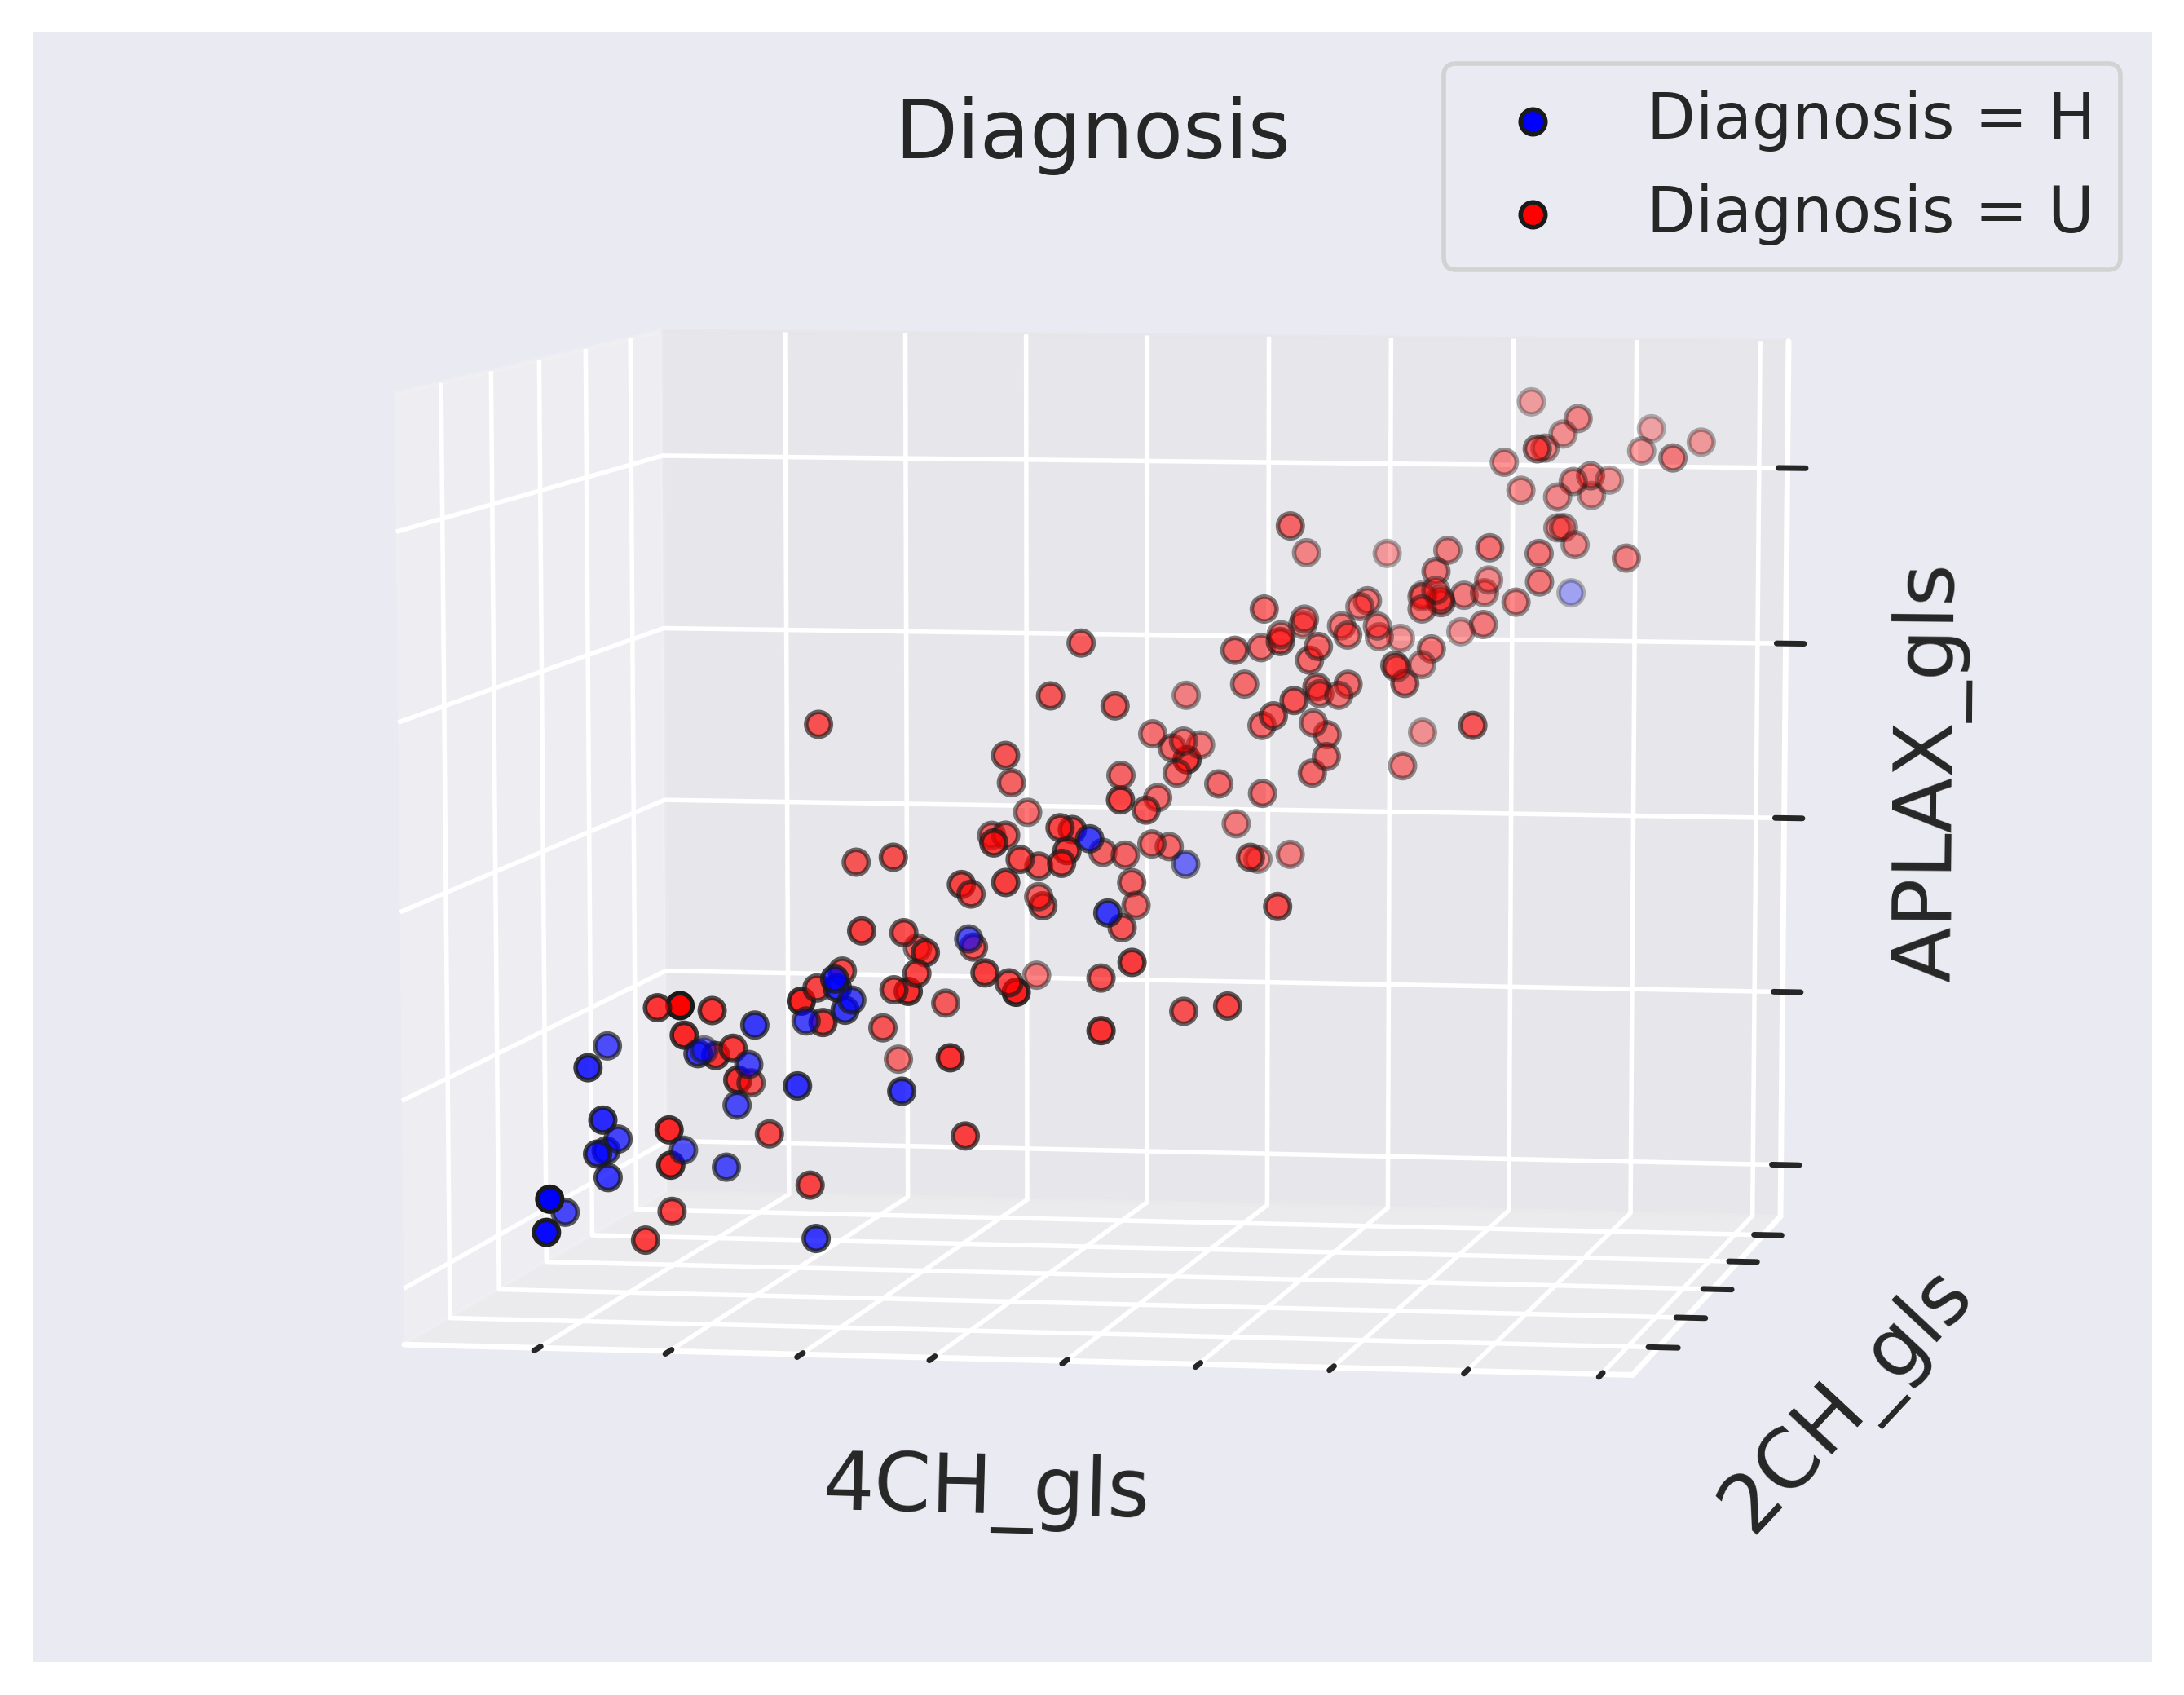
\includegraphics[width=0.99\textwidth]{results/pd/scatter_gls_indication_bin.png}
        \caption{Patient Diagnosis.}
        \label{fig:scatter_gls_ef_hf}
    \end{subfigure}
    \begin{subfigure}[b]{0.49\textwidth}
        \centering
        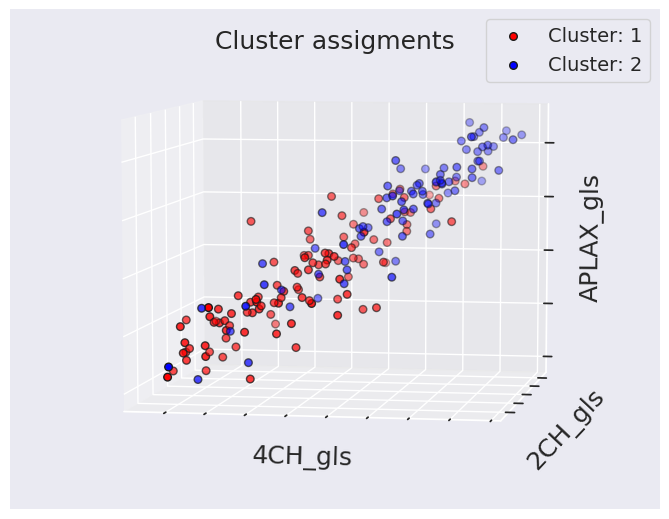
\includegraphics[width=0.99\textwidth]{results/pd/scatter_gls_EF_ward2.png}
        \caption{\textit{GLS-EF Ward/2} cluster assignments.}
        \label{fig:scatter_gls_ef_ward2}
    \end{subfigure}\\
    \begin{subfigure}[b]{0.49\textwidth}
        \centering
        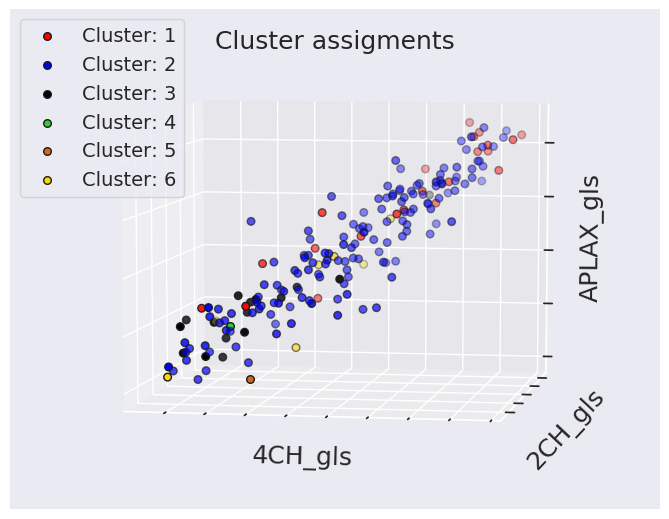
\includegraphics[width=0.99\textwidth]{results/pd/scatter_gls_average6.png}
        \caption{\textit{GLS Average/6} cluster assignments.}
        \label{fig:scatter_gls_ef_complete2}
    \end{subfigure}
    \begin{subfigure}[b]{0.49\textwidth}
        \centering
        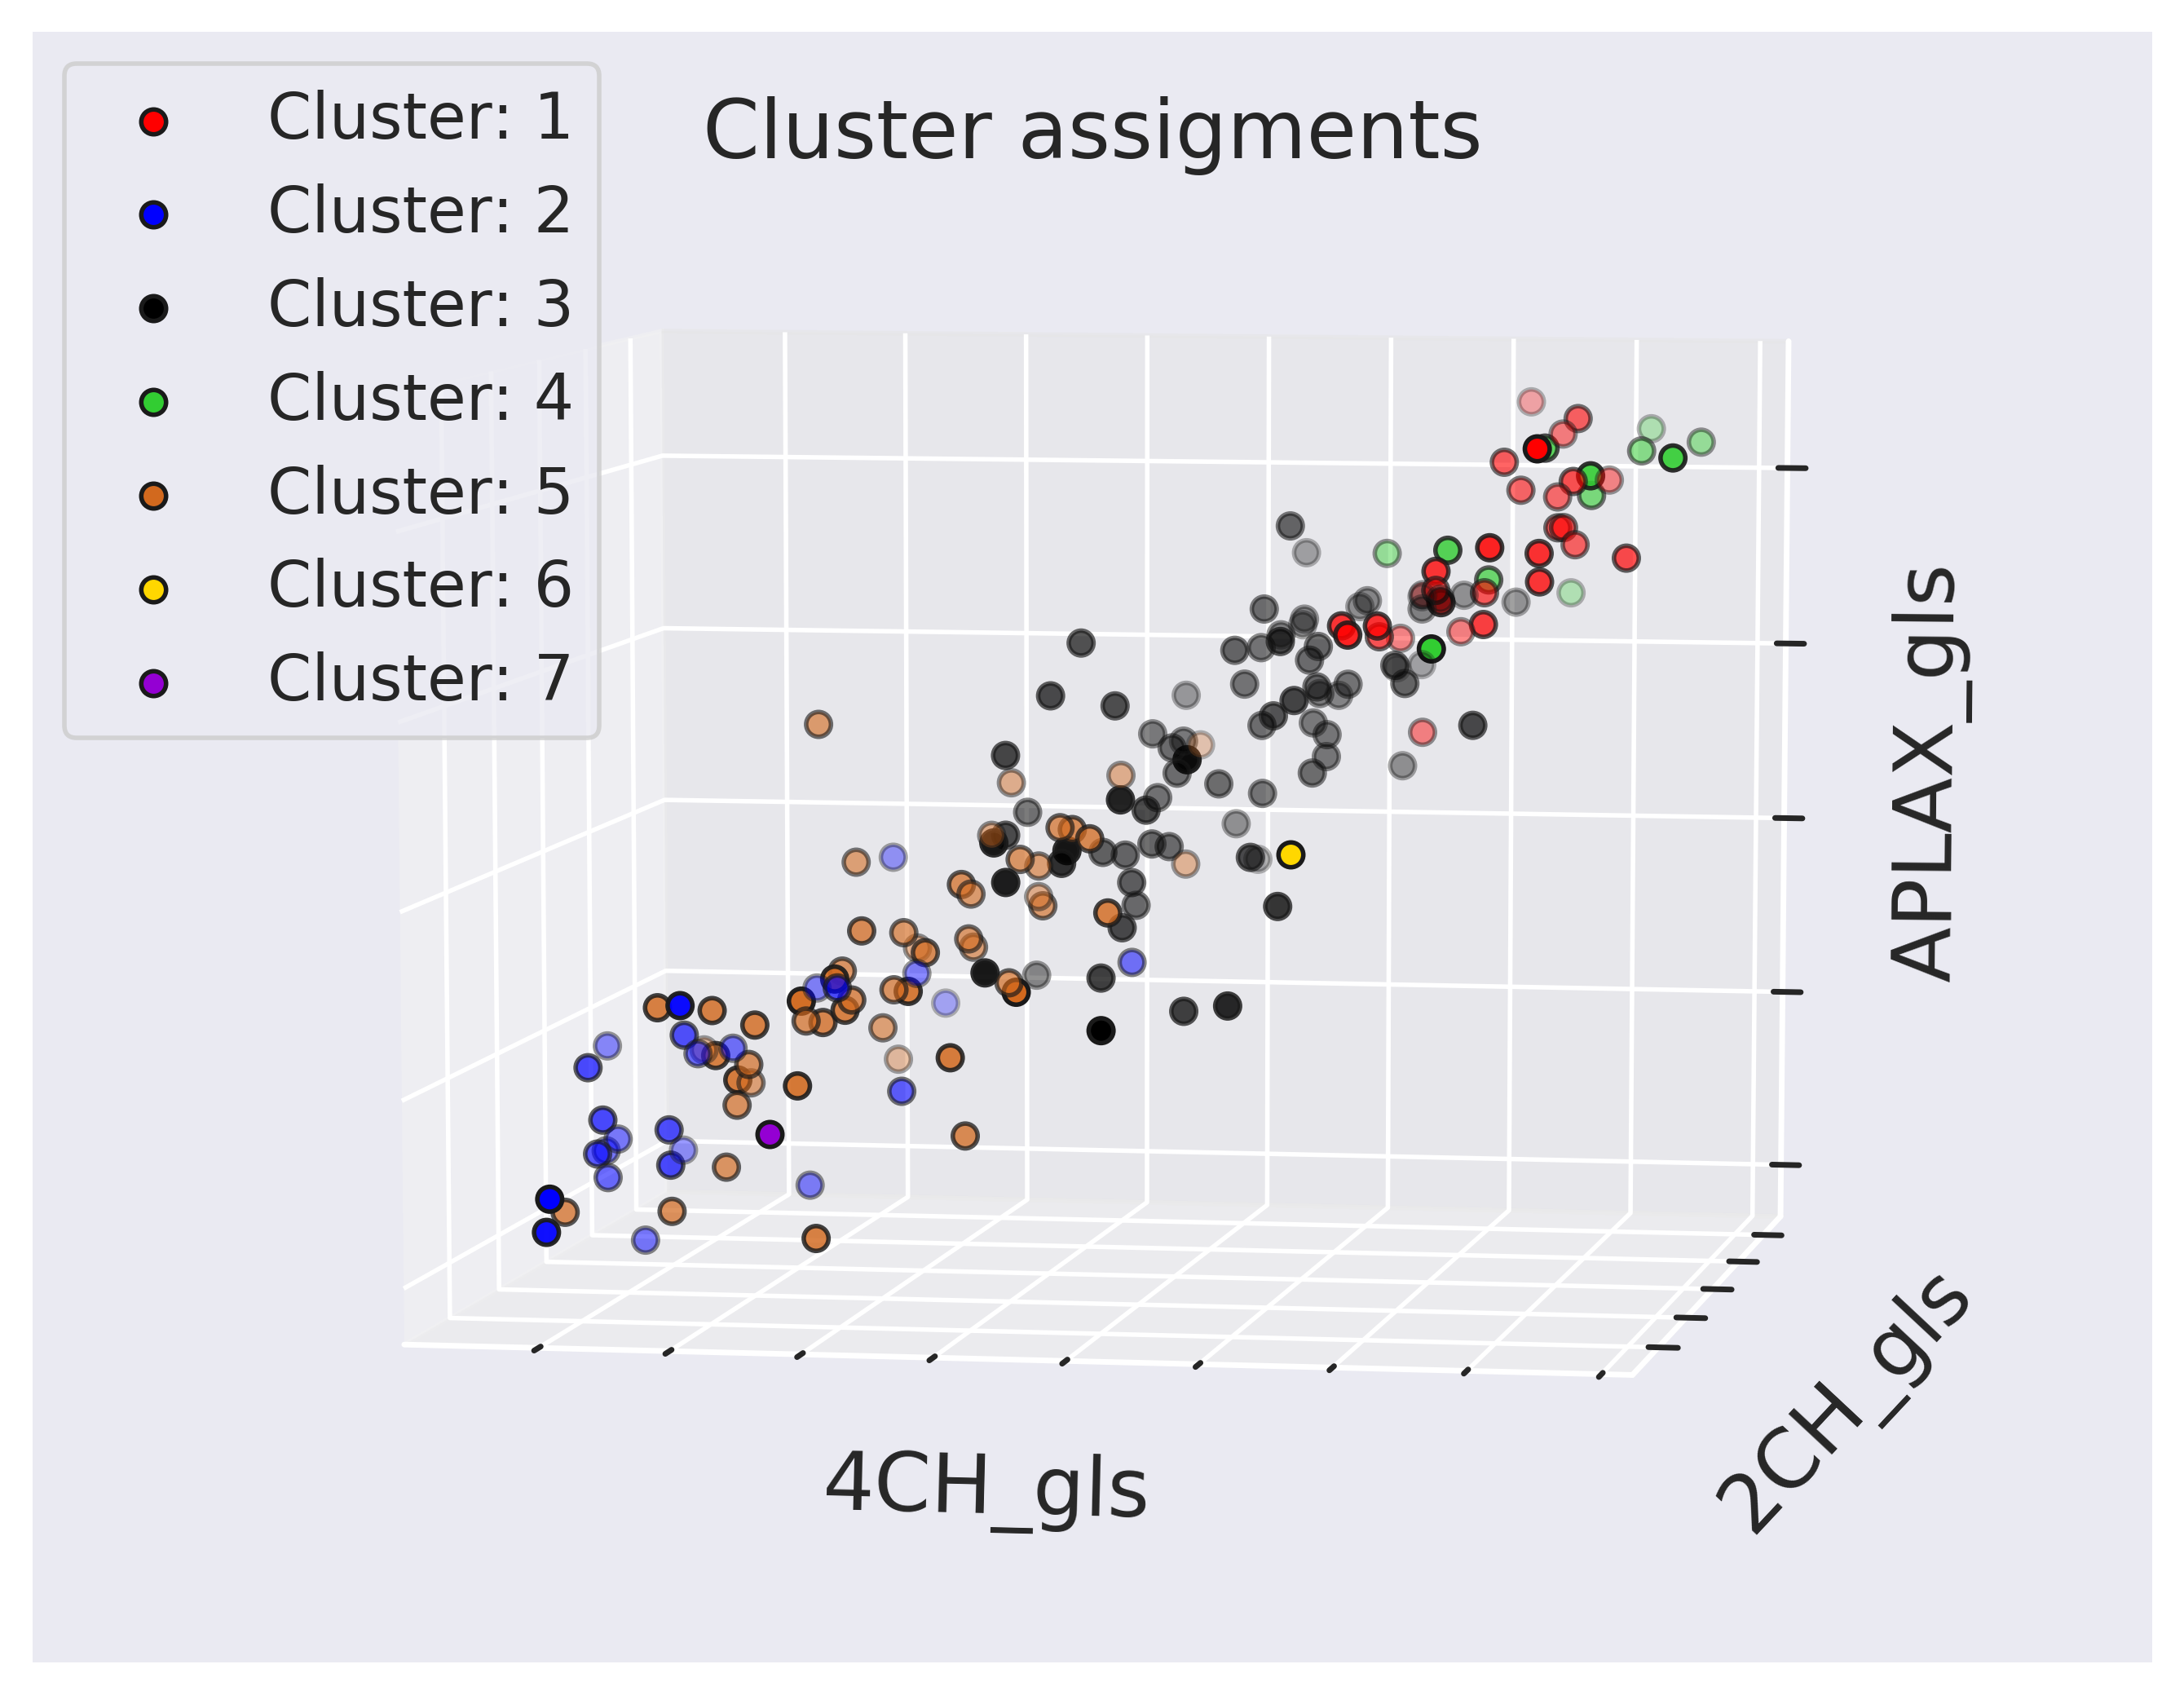
\includegraphics[width=0.99\textwidth]{results/pd/scatter_gls_average7.png}
        \caption{\textit{GLS Average/7} cluster assignments.}
        \label{fig:scatter_gls_ef_average2}
    \end{subfigure}
    \caption{Scatterplot of peak GLS values in each view. Colors in the of the different dots are given by heart failure diagnosis, and cluster assignments of 
             \textit{gls-EF/ward/2}, \textit{average/6} and \textit{average/7} methods. Numbers are not included on the axes because the point of the figure is to illustrate the separability 
             of clusters, and patient diagnosis.}
             \label{fig:scatter_gls_ef_hf_cluster_assignments}
\end{figure}

\newpage

\subsection{Deep Neural Network}

\begin{figure}[htb]
    \centering
    % \includegraphics[width=\textwidth]{results/dl_ind_dor_sens_spec_dist.png}
    %% Creator: Matplotlib, PGF backend
%%
%% To include the figure in your LaTeX document, write
%%   \input{<filename>.pgf}
%%
%% Make sure the required packages are loaded in your preamble
%%   \usepackage{pgf}
%%
%% Figures using additional raster images can only be included by \input if
%% they are in the same directory as the main LaTeX file. For loading figures
%% from other directories you can use the `import` package
%%   \usepackage{import}
%% and then include the figures with
%%   \import{<path to file>}{<filename>.pgf}
%%
%% Matplotlib used the following preamble
%%
\begingroup%
\makeatletter%
\begin{pgfpicture}%
\pgfpathrectangle{\pgfpointorigin}{\pgfqpoint{6.439273in}{2.540000in}}%
\pgfusepath{use as bounding box, clip}%
\begin{pgfscope}%
\pgfsetbuttcap%
\pgfsetmiterjoin%
\definecolor{currentfill}{rgb}{1.000000,1.000000,1.000000}%
\pgfsetfillcolor{currentfill}%
\pgfsetlinewidth{0.000000pt}%
\definecolor{currentstroke}{rgb}{1.000000,1.000000,1.000000}%
\pgfsetstrokecolor{currentstroke}%
\pgfsetdash{}{0pt}%
\pgfpathmoveto{\pgfqpoint{0.000000in}{0.000000in}}%
\pgfpathlineto{\pgfqpoint{6.439273in}{0.000000in}}%
\pgfpathlineto{\pgfqpoint{6.439273in}{2.540000in}}%
\pgfpathlineto{\pgfqpoint{0.000000in}{2.540000in}}%
\pgfpathclose%
\pgfusepath{fill}%
\end{pgfscope}%
\begin{pgfscope}%
\pgfsetbuttcap%
\pgfsetmiterjoin%
\definecolor{currentfill}{rgb}{0.917647,0.917647,0.949020}%
\pgfsetfillcolor{currentfill}%
\pgfsetlinewidth{0.000000pt}%
\definecolor{currentstroke}{rgb}{0.000000,0.000000,0.000000}%
\pgfsetstrokecolor{currentstroke}%
\pgfsetstrokeopacity{0.000000}%
\pgfsetdash{}{0pt}%
\pgfpathmoveto{\pgfqpoint{0.693056in}{0.557870in}}%
\pgfpathlineto{\pgfqpoint{3.156042in}{0.557870in}}%
\pgfpathlineto{\pgfqpoint{3.156042in}{2.242604in}}%
\pgfpathlineto{\pgfqpoint{0.693056in}{2.242604in}}%
\pgfpathclose%
\pgfusepath{fill}%
\end{pgfscope}%
\begin{pgfscope}%
\pgfpathrectangle{\pgfqpoint{0.693056in}{0.557870in}}{\pgfqpoint{2.462986in}{1.684734in}}%
\pgfusepath{clip}%
\pgfsetroundcap%
\pgfsetroundjoin%
\pgfsetlinewidth{1.003750pt}%
\definecolor{currentstroke}{rgb}{1.000000,1.000000,1.000000}%
\pgfsetstrokecolor{currentstroke}%
\pgfsetdash{}{0pt}%
\pgfpathmoveto{\pgfqpoint{0.805010in}{0.557870in}}%
\pgfpathlineto{\pgfqpoint{0.805010in}{2.242604in}}%
\pgfusepath{stroke}%
\end{pgfscope}%
\begin{pgfscope}%
\definecolor{textcolor}{rgb}{0.150000,0.150000,0.150000}%
\pgfsetstrokecolor{textcolor}%
\pgfsetfillcolor{textcolor}%
\pgftext[x=0.805010in,y=0.425926in,,top]{\color{textcolor}\sffamily\fontsize{11.000000}{13.200000}\selectfont \(\displaystyle -0.50\)}%
\end{pgfscope}%
\begin{pgfscope}%
\pgfpathrectangle{\pgfqpoint{0.693056in}{0.557870in}}{\pgfqpoint{2.462986in}{1.684734in}}%
\pgfusepath{clip}%
\pgfsetroundcap%
\pgfsetroundjoin%
\pgfsetlinewidth{1.003750pt}%
\definecolor{currentstroke}{rgb}{1.000000,1.000000,1.000000}%
\pgfsetstrokecolor{currentstroke}%
\pgfsetdash{}{0pt}%
\pgfpathmoveto{\pgfqpoint{1.364779in}{0.557870in}}%
\pgfpathlineto{\pgfqpoint{1.364779in}{2.242604in}}%
\pgfusepath{stroke}%
\end{pgfscope}%
\begin{pgfscope}%
\definecolor{textcolor}{rgb}{0.150000,0.150000,0.150000}%
\pgfsetstrokecolor{textcolor}%
\pgfsetfillcolor{textcolor}%
\pgftext[x=1.364779in,y=0.425926in,,top]{\color{textcolor}\sffamily\fontsize{11.000000}{13.200000}\selectfont \(\displaystyle -0.25\)}%
\end{pgfscope}%
\begin{pgfscope}%
\pgfpathrectangle{\pgfqpoint{0.693056in}{0.557870in}}{\pgfqpoint{2.462986in}{1.684734in}}%
\pgfusepath{clip}%
\pgfsetroundcap%
\pgfsetroundjoin%
\pgfsetlinewidth{1.003750pt}%
\definecolor{currentstroke}{rgb}{1.000000,1.000000,1.000000}%
\pgfsetstrokecolor{currentstroke}%
\pgfsetdash{}{0pt}%
\pgfpathmoveto{\pgfqpoint{1.924549in}{0.557870in}}%
\pgfpathlineto{\pgfqpoint{1.924549in}{2.242604in}}%
\pgfusepath{stroke}%
\end{pgfscope}%
\begin{pgfscope}%
\definecolor{textcolor}{rgb}{0.150000,0.150000,0.150000}%
\pgfsetstrokecolor{textcolor}%
\pgfsetfillcolor{textcolor}%
\pgftext[x=1.924549in,y=0.425926in,,top]{\color{textcolor}\sffamily\fontsize{11.000000}{13.200000}\selectfont \(\displaystyle 0.00\)}%
\end{pgfscope}%
\begin{pgfscope}%
\pgfpathrectangle{\pgfqpoint{0.693056in}{0.557870in}}{\pgfqpoint{2.462986in}{1.684734in}}%
\pgfusepath{clip}%
\pgfsetroundcap%
\pgfsetroundjoin%
\pgfsetlinewidth{1.003750pt}%
\definecolor{currentstroke}{rgb}{1.000000,1.000000,1.000000}%
\pgfsetstrokecolor{currentstroke}%
\pgfsetdash{}{0pt}%
\pgfpathmoveto{\pgfqpoint{2.484318in}{0.557870in}}%
\pgfpathlineto{\pgfqpoint{2.484318in}{2.242604in}}%
\pgfusepath{stroke}%
\end{pgfscope}%
\begin{pgfscope}%
\definecolor{textcolor}{rgb}{0.150000,0.150000,0.150000}%
\pgfsetstrokecolor{textcolor}%
\pgfsetfillcolor{textcolor}%
\pgftext[x=2.484318in,y=0.425926in,,top]{\color{textcolor}\sffamily\fontsize{11.000000}{13.200000}\selectfont \(\displaystyle 0.25\)}%
\end{pgfscope}%
\begin{pgfscope}%
\pgfpathrectangle{\pgfqpoint{0.693056in}{0.557870in}}{\pgfqpoint{2.462986in}{1.684734in}}%
\pgfusepath{clip}%
\pgfsetroundcap%
\pgfsetroundjoin%
\pgfsetlinewidth{1.003750pt}%
\definecolor{currentstroke}{rgb}{1.000000,1.000000,1.000000}%
\pgfsetstrokecolor{currentstroke}%
\pgfsetdash{}{0pt}%
\pgfpathmoveto{\pgfqpoint{3.044088in}{0.557870in}}%
\pgfpathlineto{\pgfqpoint{3.044088in}{2.242604in}}%
\pgfusepath{stroke}%
\end{pgfscope}%
\begin{pgfscope}%
\definecolor{textcolor}{rgb}{0.150000,0.150000,0.150000}%
\pgfsetstrokecolor{textcolor}%
\pgfsetfillcolor{textcolor}%
\pgftext[x=3.044088in,y=0.425926in,,top]{\color{textcolor}\sffamily\fontsize{11.000000}{13.200000}\selectfont \(\displaystyle 0.50\)}%
\end{pgfscope}%
\begin{pgfscope}%
\definecolor{textcolor}{rgb}{0.150000,0.150000,0.150000}%
\pgfsetstrokecolor{textcolor}%
\pgfsetfillcolor{textcolor}%
\pgftext[x=1.924549in,y=0.235185in,,top]{\color{textcolor}\sffamily\fontsize{11.000000}{13.200000}\selectfont DOR}%
\end{pgfscope}%
\begin{pgfscope}%
\pgfpathrectangle{\pgfqpoint{0.693056in}{0.557870in}}{\pgfqpoint{2.462986in}{1.684734in}}%
\pgfusepath{clip}%
\pgfsetroundcap%
\pgfsetroundjoin%
\pgfsetlinewidth{1.003750pt}%
\definecolor{currentstroke}{rgb}{1.000000,1.000000,1.000000}%
\pgfsetstrokecolor{currentstroke}%
\pgfsetdash{}{0pt}%
\pgfpathmoveto{\pgfqpoint{0.693056in}{0.557870in}}%
\pgfpathlineto{\pgfqpoint{3.156042in}{0.557870in}}%
\pgfusepath{stroke}%
\end{pgfscope}%
\begin{pgfscope}%
\definecolor{textcolor}{rgb}{0.150000,0.150000,0.150000}%
\pgfsetstrokecolor{textcolor}%
\pgfsetfillcolor{textcolor}%
\pgftext[x=0.290741in,y=0.505064in,left,base]{\color{textcolor}\sffamily\fontsize{11.000000}{13.200000}\selectfont \(\displaystyle 0.00\)}%
\end{pgfscope}%
\begin{pgfscope}%
\pgfpathrectangle{\pgfqpoint{0.693056in}{0.557870in}}{\pgfqpoint{2.462986in}{1.684734in}}%
\pgfusepath{clip}%
\pgfsetroundcap%
\pgfsetroundjoin%
\pgfsetlinewidth{1.003750pt}%
\definecolor{currentstroke}{rgb}{1.000000,1.000000,1.000000}%
\pgfsetstrokecolor{currentstroke}%
\pgfsetdash{}{0pt}%
\pgfpathmoveto{\pgfqpoint{0.693056in}{0.958997in}}%
\pgfpathlineto{\pgfqpoint{3.156042in}{0.958997in}}%
\pgfusepath{stroke}%
\end{pgfscope}%
\begin{pgfscope}%
\definecolor{textcolor}{rgb}{0.150000,0.150000,0.150000}%
\pgfsetstrokecolor{textcolor}%
\pgfsetfillcolor{textcolor}%
\pgftext[x=0.290741in,y=0.906191in,left,base]{\color{textcolor}\sffamily\fontsize{11.000000}{13.200000}\selectfont \(\displaystyle 0.25\)}%
\end{pgfscope}%
\begin{pgfscope}%
\pgfpathrectangle{\pgfqpoint{0.693056in}{0.557870in}}{\pgfqpoint{2.462986in}{1.684734in}}%
\pgfusepath{clip}%
\pgfsetroundcap%
\pgfsetroundjoin%
\pgfsetlinewidth{1.003750pt}%
\definecolor{currentstroke}{rgb}{1.000000,1.000000,1.000000}%
\pgfsetstrokecolor{currentstroke}%
\pgfsetdash{}{0pt}%
\pgfpathmoveto{\pgfqpoint{0.693056in}{1.360125in}}%
\pgfpathlineto{\pgfqpoint{3.156042in}{1.360125in}}%
\pgfusepath{stroke}%
\end{pgfscope}%
\begin{pgfscope}%
\definecolor{textcolor}{rgb}{0.150000,0.150000,0.150000}%
\pgfsetstrokecolor{textcolor}%
\pgfsetfillcolor{textcolor}%
\pgftext[x=0.290741in,y=1.307318in,left,base]{\color{textcolor}\sffamily\fontsize{11.000000}{13.200000}\selectfont \(\displaystyle 0.50\)}%
\end{pgfscope}%
\begin{pgfscope}%
\pgfpathrectangle{\pgfqpoint{0.693056in}{0.557870in}}{\pgfqpoint{2.462986in}{1.684734in}}%
\pgfusepath{clip}%
\pgfsetroundcap%
\pgfsetroundjoin%
\pgfsetlinewidth{1.003750pt}%
\definecolor{currentstroke}{rgb}{1.000000,1.000000,1.000000}%
\pgfsetstrokecolor{currentstroke}%
\pgfsetdash{}{0pt}%
\pgfpathmoveto{\pgfqpoint{0.693056in}{1.761252in}}%
\pgfpathlineto{\pgfqpoint{3.156042in}{1.761252in}}%
\pgfusepath{stroke}%
\end{pgfscope}%
\begin{pgfscope}%
\definecolor{textcolor}{rgb}{0.150000,0.150000,0.150000}%
\pgfsetstrokecolor{textcolor}%
\pgfsetfillcolor{textcolor}%
\pgftext[x=0.290741in,y=1.708445in,left,base]{\color{textcolor}\sffamily\fontsize{11.000000}{13.200000}\selectfont \(\displaystyle 0.75\)}%
\end{pgfscope}%
\begin{pgfscope}%
\pgfpathrectangle{\pgfqpoint{0.693056in}{0.557870in}}{\pgfqpoint{2.462986in}{1.684734in}}%
\pgfusepath{clip}%
\pgfsetroundcap%
\pgfsetroundjoin%
\pgfsetlinewidth{1.003750pt}%
\definecolor{currentstroke}{rgb}{1.000000,1.000000,1.000000}%
\pgfsetstrokecolor{currentstroke}%
\pgfsetdash{}{0pt}%
\pgfpathmoveto{\pgfqpoint{0.693056in}{2.162379in}}%
\pgfpathlineto{\pgfqpoint{3.156042in}{2.162379in}}%
\pgfusepath{stroke}%
\end{pgfscope}%
\begin{pgfscope}%
\definecolor{textcolor}{rgb}{0.150000,0.150000,0.150000}%
\pgfsetstrokecolor{textcolor}%
\pgfsetfillcolor{textcolor}%
\pgftext[x=0.290741in,y=2.109572in,left,base]{\color{textcolor}\sffamily\fontsize{11.000000}{13.200000}\selectfont \(\displaystyle 1.00\)}%
\end{pgfscope}%
\begin{pgfscope}%
\definecolor{textcolor}{rgb}{0.150000,0.150000,0.150000}%
\pgfsetstrokecolor{textcolor}%
\pgfsetfillcolor{textcolor}%
\pgftext[x=0.235185in,y=1.400237in,,bottom,rotate=90.000000]{\color{textcolor}\sffamily\fontsize{11.000000}{13.200000}\selectfont Occurance}%
\end{pgfscope}%
\begin{pgfscope}%
\pgfpathrectangle{\pgfqpoint{0.693056in}{0.557870in}}{\pgfqpoint{2.462986in}{1.684734in}}%
\pgfusepath{clip}%
\pgfsetbuttcap%
\pgfsetmiterjoin%
\definecolor{currentfill}{rgb}{0.298039,0.447059,0.690196}%
\pgfsetfillcolor{currentfill}%
\pgfsetfillopacity{0.400000}%
\pgfsetlinewidth{1.003750pt}%
\definecolor{currentstroke}{rgb}{1.000000,1.000000,1.000000}%
\pgfsetstrokecolor{currentstroke}%
\pgfsetstrokeopacity{0.400000}%
\pgfsetdash{}{0pt}%
\pgfpathmoveto{\pgfqpoint{0.805010in}{0.557870in}}%
\pgfpathlineto{\pgfqpoint{1.028918in}{0.557870in}}%
\pgfpathlineto{\pgfqpoint{1.028918in}{0.557870in}}%
\pgfpathlineto{\pgfqpoint{0.805010in}{0.557870in}}%
\pgfpathclose%
\pgfusepath{stroke,fill}%
\end{pgfscope}%
\begin{pgfscope}%
\pgfpathrectangle{\pgfqpoint{0.693056in}{0.557870in}}{\pgfqpoint{2.462986in}{1.684734in}}%
\pgfusepath{clip}%
\pgfsetbuttcap%
\pgfsetmiterjoin%
\definecolor{currentfill}{rgb}{0.298039,0.447059,0.690196}%
\pgfsetfillcolor{currentfill}%
\pgfsetfillopacity{0.400000}%
\pgfsetlinewidth{1.003750pt}%
\definecolor{currentstroke}{rgb}{1.000000,1.000000,1.000000}%
\pgfsetstrokecolor{currentstroke}%
\pgfsetstrokeopacity{0.400000}%
\pgfsetdash{}{0pt}%
\pgfpathmoveto{\pgfqpoint{1.028918in}{0.557870in}}%
\pgfpathlineto{\pgfqpoint{1.252825in}{0.557870in}}%
\pgfpathlineto{\pgfqpoint{1.252825in}{0.557870in}}%
\pgfpathlineto{\pgfqpoint{1.028918in}{0.557870in}}%
\pgfpathclose%
\pgfusepath{stroke,fill}%
\end{pgfscope}%
\begin{pgfscope}%
\pgfpathrectangle{\pgfqpoint{0.693056in}{0.557870in}}{\pgfqpoint{2.462986in}{1.684734in}}%
\pgfusepath{clip}%
\pgfsetbuttcap%
\pgfsetmiterjoin%
\definecolor{currentfill}{rgb}{0.298039,0.447059,0.690196}%
\pgfsetfillcolor{currentfill}%
\pgfsetfillopacity{0.400000}%
\pgfsetlinewidth{1.003750pt}%
\definecolor{currentstroke}{rgb}{1.000000,1.000000,1.000000}%
\pgfsetstrokecolor{currentstroke}%
\pgfsetstrokeopacity{0.400000}%
\pgfsetdash{}{0pt}%
\pgfpathmoveto{\pgfqpoint{1.252825in}{0.557870in}}%
\pgfpathlineto{\pgfqpoint{1.476733in}{0.557870in}}%
\pgfpathlineto{\pgfqpoint{1.476733in}{0.557870in}}%
\pgfpathlineto{\pgfqpoint{1.252825in}{0.557870in}}%
\pgfpathclose%
\pgfusepath{stroke,fill}%
\end{pgfscope}%
\begin{pgfscope}%
\pgfpathrectangle{\pgfqpoint{0.693056in}{0.557870in}}{\pgfqpoint{2.462986in}{1.684734in}}%
\pgfusepath{clip}%
\pgfsetbuttcap%
\pgfsetmiterjoin%
\definecolor{currentfill}{rgb}{0.298039,0.447059,0.690196}%
\pgfsetfillcolor{currentfill}%
\pgfsetfillopacity{0.400000}%
\pgfsetlinewidth{1.003750pt}%
\definecolor{currentstroke}{rgb}{1.000000,1.000000,1.000000}%
\pgfsetstrokecolor{currentstroke}%
\pgfsetstrokeopacity{0.400000}%
\pgfsetdash{}{0pt}%
\pgfpathmoveto{\pgfqpoint{1.476733in}{0.557870in}}%
\pgfpathlineto{\pgfqpoint{1.700641in}{0.557870in}}%
\pgfpathlineto{\pgfqpoint{1.700641in}{0.557870in}}%
\pgfpathlineto{\pgfqpoint{1.476733in}{0.557870in}}%
\pgfpathclose%
\pgfusepath{stroke,fill}%
\end{pgfscope}%
\begin{pgfscope}%
\pgfpathrectangle{\pgfqpoint{0.693056in}{0.557870in}}{\pgfqpoint{2.462986in}{1.684734in}}%
\pgfusepath{clip}%
\pgfsetbuttcap%
\pgfsetmiterjoin%
\definecolor{currentfill}{rgb}{0.298039,0.447059,0.690196}%
\pgfsetfillcolor{currentfill}%
\pgfsetfillopacity{0.400000}%
\pgfsetlinewidth{1.003750pt}%
\definecolor{currentstroke}{rgb}{1.000000,1.000000,1.000000}%
\pgfsetstrokecolor{currentstroke}%
\pgfsetstrokeopacity{0.400000}%
\pgfsetdash{}{0pt}%
\pgfpathmoveto{\pgfqpoint{1.700641in}{0.557870in}}%
\pgfpathlineto{\pgfqpoint{1.924549in}{0.557870in}}%
\pgfpathlineto{\pgfqpoint{1.924549in}{0.557870in}}%
\pgfpathlineto{\pgfqpoint{1.700641in}{0.557870in}}%
\pgfpathclose%
\pgfusepath{stroke,fill}%
\end{pgfscope}%
\begin{pgfscope}%
\pgfpathrectangle{\pgfqpoint{0.693056in}{0.557870in}}{\pgfqpoint{2.462986in}{1.684734in}}%
\pgfusepath{clip}%
\pgfsetbuttcap%
\pgfsetmiterjoin%
\definecolor{currentfill}{rgb}{0.298039,0.447059,0.690196}%
\pgfsetfillcolor{currentfill}%
\pgfsetfillopacity{0.400000}%
\pgfsetlinewidth{1.003750pt}%
\definecolor{currentstroke}{rgb}{1.000000,1.000000,1.000000}%
\pgfsetstrokecolor{currentstroke}%
\pgfsetstrokeopacity{0.400000}%
\pgfsetdash{}{0pt}%
\pgfpathmoveto{\pgfqpoint{1.924549in}{0.557870in}}%
\pgfpathlineto{\pgfqpoint{2.148457in}{0.557870in}}%
\pgfpathlineto{\pgfqpoint{2.148457in}{2.162379in}}%
\pgfpathlineto{\pgfqpoint{1.924549in}{2.162379in}}%
\pgfpathclose%
\pgfusepath{stroke,fill}%
\end{pgfscope}%
\begin{pgfscope}%
\pgfpathrectangle{\pgfqpoint{0.693056in}{0.557870in}}{\pgfqpoint{2.462986in}{1.684734in}}%
\pgfusepath{clip}%
\pgfsetbuttcap%
\pgfsetmiterjoin%
\definecolor{currentfill}{rgb}{0.298039,0.447059,0.690196}%
\pgfsetfillcolor{currentfill}%
\pgfsetfillopacity{0.400000}%
\pgfsetlinewidth{1.003750pt}%
\definecolor{currentstroke}{rgb}{1.000000,1.000000,1.000000}%
\pgfsetstrokecolor{currentstroke}%
\pgfsetstrokeopacity{0.400000}%
\pgfsetdash{}{0pt}%
\pgfpathmoveto{\pgfqpoint{2.148457in}{0.557870in}}%
\pgfpathlineto{\pgfqpoint{2.372364in}{0.557870in}}%
\pgfpathlineto{\pgfqpoint{2.372364in}{0.557870in}}%
\pgfpathlineto{\pgfqpoint{2.148457in}{0.557870in}}%
\pgfpathclose%
\pgfusepath{stroke,fill}%
\end{pgfscope}%
\begin{pgfscope}%
\pgfpathrectangle{\pgfqpoint{0.693056in}{0.557870in}}{\pgfqpoint{2.462986in}{1.684734in}}%
\pgfusepath{clip}%
\pgfsetbuttcap%
\pgfsetmiterjoin%
\definecolor{currentfill}{rgb}{0.298039,0.447059,0.690196}%
\pgfsetfillcolor{currentfill}%
\pgfsetfillopacity{0.400000}%
\pgfsetlinewidth{1.003750pt}%
\definecolor{currentstroke}{rgb}{1.000000,1.000000,1.000000}%
\pgfsetstrokecolor{currentstroke}%
\pgfsetstrokeopacity{0.400000}%
\pgfsetdash{}{0pt}%
\pgfpathmoveto{\pgfqpoint{2.372364in}{0.557870in}}%
\pgfpathlineto{\pgfqpoint{2.596272in}{0.557870in}}%
\pgfpathlineto{\pgfqpoint{2.596272in}{0.557870in}}%
\pgfpathlineto{\pgfqpoint{2.372364in}{0.557870in}}%
\pgfpathclose%
\pgfusepath{stroke,fill}%
\end{pgfscope}%
\begin{pgfscope}%
\pgfpathrectangle{\pgfqpoint{0.693056in}{0.557870in}}{\pgfqpoint{2.462986in}{1.684734in}}%
\pgfusepath{clip}%
\pgfsetbuttcap%
\pgfsetmiterjoin%
\definecolor{currentfill}{rgb}{0.298039,0.447059,0.690196}%
\pgfsetfillcolor{currentfill}%
\pgfsetfillopacity{0.400000}%
\pgfsetlinewidth{1.003750pt}%
\definecolor{currentstroke}{rgb}{1.000000,1.000000,1.000000}%
\pgfsetstrokecolor{currentstroke}%
\pgfsetstrokeopacity{0.400000}%
\pgfsetdash{}{0pt}%
\pgfpathmoveto{\pgfqpoint{2.596272in}{0.557870in}}%
\pgfpathlineto{\pgfqpoint{2.820180in}{0.557870in}}%
\pgfpathlineto{\pgfqpoint{2.820180in}{0.557870in}}%
\pgfpathlineto{\pgfqpoint{2.596272in}{0.557870in}}%
\pgfpathclose%
\pgfusepath{stroke,fill}%
\end{pgfscope}%
\begin{pgfscope}%
\pgfpathrectangle{\pgfqpoint{0.693056in}{0.557870in}}{\pgfqpoint{2.462986in}{1.684734in}}%
\pgfusepath{clip}%
\pgfsetbuttcap%
\pgfsetmiterjoin%
\definecolor{currentfill}{rgb}{0.298039,0.447059,0.690196}%
\pgfsetfillcolor{currentfill}%
\pgfsetfillopacity{0.400000}%
\pgfsetlinewidth{1.003750pt}%
\definecolor{currentstroke}{rgb}{1.000000,1.000000,1.000000}%
\pgfsetstrokecolor{currentstroke}%
\pgfsetstrokeopacity{0.400000}%
\pgfsetdash{}{0pt}%
\pgfpathmoveto{\pgfqpoint{2.820180in}{0.557870in}}%
\pgfpathlineto{\pgfqpoint{3.044088in}{0.557870in}}%
\pgfpathlineto{\pgfqpoint{3.044088in}{0.557870in}}%
\pgfpathlineto{\pgfqpoint{2.820180in}{0.557870in}}%
\pgfpathclose%
\pgfusepath{stroke,fill}%
\end{pgfscope}%
\begin{pgfscope}%
\pgfsetrectcap%
\pgfsetmiterjoin%
\pgfsetlinewidth{1.254687pt}%
\definecolor{currentstroke}{rgb}{1.000000,1.000000,1.000000}%
\pgfsetstrokecolor{currentstroke}%
\pgfsetdash{}{0pt}%
\pgfpathmoveto{\pgfqpoint{0.693056in}{0.557870in}}%
\pgfpathlineto{\pgfqpoint{0.693056in}{2.242604in}}%
\pgfusepath{stroke}%
\end{pgfscope}%
\begin{pgfscope}%
\pgfsetrectcap%
\pgfsetmiterjoin%
\pgfsetlinewidth{1.254687pt}%
\definecolor{currentstroke}{rgb}{1.000000,1.000000,1.000000}%
\pgfsetstrokecolor{currentstroke}%
\pgfsetdash{}{0pt}%
\pgfpathmoveto{\pgfqpoint{3.156042in}{0.557870in}}%
\pgfpathlineto{\pgfqpoint{3.156042in}{2.242604in}}%
\pgfusepath{stroke}%
\end{pgfscope}%
\begin{pgfscope}%
\pgfsetrectcap%
\pgfsetmiterjoin%
\pgfsetlinewidth{1.254687pt}%
\definecolor{currentstroke}{rgb}{1.000000,1.000000,1.000000}%
\pgfsetstrokecolor{currentstroke}%
\pgfsetdash{}{0pt}%
\pgfpathmoveto{\pgfqpoint{0.693056in}{0.557870in}}%
\pgfpathlineto{\pgfqpoint{3.156042in}{0.557870in}}%
\pgfusepath{stroke}%
\end{pgfscope}%
\begin{pgfscope}%
\pgfsetrectcap%
\pgfsetmiterjoin%
\pgfsetlinewidth{1.254687pt}%
\definecolor{currentstroke}{rgb}{1.000000,1.000000,1.000000}%
\pgfsetstrokecolor{currentstroke}%
\pgfsetdash{}{0pt}%
\pgfpathmoveto{\pgfqpoint{0.693056in}{2.242604in}}%
\pgfpathlineto{\pgfqpoint{3.156042in}{2.242604in}}%
\pgfusepath{stroke}%
\end{pgfscope}%
\begin{pgfscope}%
\definecolor{textcolor}{rgb}{0.150000,0.150000,0.150000}%
\pgfsetstrokecolor{textcolor}%
\pgfsetfillcolor{textcolor}%
\pgftext[x=1.924549in,y=2.325938in,,base]{\color{textcolor}\sffamily\fontsize{11.000000}{13.200000}\selectfont (a)}%
\end{pgfscope}%
\begin{pgfscope}%
\pgfsetbuttcap%
\pgfsetmiterjoin%
\definecolor{currentfill}{rgb}{0.917647,0.917647,0.949020}%
\pgfsetfillcolor{currentfill}%
\pgfsetlinewidth{0.000000pt}%
\definecolor{currentstroke}{rgb}{0.000000,0.000000,0.000000}%
\pgfsetstrokecolor{currentstroke}%
\pgfsetstrokeopacity{0.000000}%
\pgfsetdash{}{0pt}%
\pgfpathmoveto{\pgfqpoint{3.853056in}{0.557870in}}%
\pgfpathlineto{\pgfqpoint{6.316042in}{0.557870in}}%
\pgfpathlineto{\pgfqpoint{6.316042in}{2.242604in}}%
\pgfpathlineto{\pgfqpoint{3.853056in}{2.242604in}}%
\pgfpathclose%
\pgfusepath{fill}%
\end{pgfscope}%
\begin{pgfscope}%
\pgfpathrectangle{\pgfqpoint{3.853056in}{0.557870in}}{\pgfqpoint{2.462986in}{1.684734in}}%
\pgfusepath{clip}%
\pgfsetroundcap%
\pgfsetroundjoin%
\pgfsetlinewidth{1.003750pt}%
\definecolor{currentstroke}{rgb}{1.000000,1.000000,1.000000}%
\pgfsetstrokecolor{currentstroke}%
\pgfsetdash{}{0pt}%
\pgfpathmoveto{\pgfqpoint{3.965010in}{0.557870in}}%
\pgfpathlineto{\pgfqpoint{3.965010in}{2.242604in}}%
\pgfusepath{stroke}%
\end{pgfscope}%
\begin{pgfscope}%
\definecolor{textcolor}{rgb}{0.150000,0.150000,0.150000}%
\pgfsetstrokecolor{textcolor}%
\pgfsetfillcolor{textcolor}%
\pgftext[x=3.965010in,y=0.425926in,,top]{\color{textcolor}\sffamily\fontsize{11.000000}{13.200000}\selectfont \(\displaystyle 0.00\)}%
\end{pgfscope}%
\begin{pgfscope}%
\pgfpathrectangle{\pgfqpoint{3.853056in}{0.557870in}}{\pgfqpoint{2.462986in}{1.684734in}}%
\pgfusepath{clip}%
\pgfsetroundcap%
\pgfsetroundjoin%
\pgfsetlinewidth{1.003750pt}%
\definecolor{currentstroke}{rgb}{1.000000,1.000000,1.000000}%
\pgfsetstrokecolor{currentstroke}%
\pgfsetdash{}{0pt}%
\pgfpathmoveto{\pgfqpoint{4.524779in}{0.557870in}}%
\pgfpathlineto{\pgfqpoint{4.524779in}{2.242604in}}%
\pgfusepath{stroke}%
\end{pgfscope}%
\begin{pgfscope}%
\definecolor{textcolor}{rgb}{0.150000,0.150000,0.150000}%
\pgfsetstrokecolor{textcolor}%
\pgfsetfillcolor{textcolor}%
\pgftext[x=4.524779in,y=0.425926in,,top]{\color{textcolor}\sffamily\fontsize{11.000000}{13.200000}\selectfont \(\displaystyle 0.25\)}%
\end{pgfscope}%
\begin{pgfscope}%
\pgfpathrectangle{\pgfqpoint{3.853056in}{0.557870in}}{\pgfqpoint{2.462986in}{1.684734in}}%
\pgfusepath{clip}%
\pgfsetroundcap%
\pgfsetroundjoin%
\pgfsetlinewidth{1.003750pt}%
\definecolor{currentstroke}{rgb}{1.000000,1.000000,1.000000}%
\pgfsetstrokecolor{currentstroke}%
\pgfsetdash{}{0pt}%
\pgfpathmoveto{\pgfqpoint{5.084549in}{0.557870in}}%
\pgfpathlineto{\pgfqpoint{5.084549in}{2.242604in}}%
\pgfusepath{stroke}%
\end{pgfscope}%
\begin{pgfscope}%
\definecolor{textcolor}{rgb}{0.150000,0.150000,0.150000}%
\pgfsetstrokecolor{textcolor}%
\pgfsetfillcolor{textcolor}%
\pgftext[x=5.084549in,y=0.425926in,,top]{\color{textcolor}\sffamily\fontsize{11.000000}{13.200000}\selectfont \(\displaystyle 0.50\)}%
\end{pgfscope}%
\begin{pgfscope}%
\pgfpathrectangle{\pgfqpoint{3.853056in}{0.557870in}}{\pgfqpoint{2.462986in}{1.684734in}}%
\pgfusepath{clip}%
\pgfsetroundcap%
\pgfsetroundjoin%
\pgfsetlinewidth{1.003750pt}%
\definecolor{currentstroke}{rgb}{1.000000,1.000000,1.000000}%
\pgfsetstrokecolor{currentstroke}%
\pgfsetdash{}{0pt}%
\pgfpathmoveto{\pgfqpoint{5.644318in}{0.557870in}}%
\pgfpathlineto{\pgfqpoint{5.644318in}{2.242604in}}%
\pgfusepath{stroke}%
\end{pgfscope}%
\begin{pgfscope}%
\definecolor{textcolor}{rgb}{0.150000,0.150000,0.150000}%
\pgfsetstrokecolor{textcolor}%
\pgfsetfillcolor{textcolor}%
\pgftext[x=5.644318in,y=0.425926in,,top]{\color{textcolor}\sffamily\fontsize{11.000000}{13.200000}\selectfont \(\displaystyle 0.75\)}%
\end{pgfscope}%
\begin{pgfscope}%
\pgfpathrectangle{\pgfqpoint{3.853056in}{0.557870in}}{\pgfqpoint{2.462986in}{1.684734in}}%
\pgfusepath{clip}%
\pgfsetroundcap%
\pgfsetroundjoin%
\pgfsetlinewidth{1.003750pt}%
\definecolor{currentstroke}{rgb}{1.000000,1.000000,1.000000}%
\pgfsetstrokecolor{currentstroke}%
\pgfsetdash{}{0pt}%
\pgfpathmoveto{\pgfqpoint{6.204088in}{0.557870in}}%
\pgfpathlineto{\pgfqpoint{6.204088in}{2.242604in}}%
\pgfusepath{stroke}%
\end{pgfscope}%
\begin{pgfscope}%
\definecolor{textcolor}{rgb}{0.150000,0.150000,0.150000}%
\pgfsetstrokecolor{textcolor}%
\pgfsetfillcolor{textcolor}%
\pgftext[x=6.204088in,y=0.425926in,,top]{\color{textcolor}\sffamily\fontsize{11.000000}{13.200000}\selectfont \(\displaystyle 1.00\)}%
\end{pgfscope}%
\begin{pgfscope}%
\definecolor{textcolor}{rgb}{0.150000,0.150000,0.150000}%
\pgfsetstrokecolor{textcolor}%
\pgfsetfillcolor{textcolor}%
\pgftext[x=5.084549in,y=0.235185in,,top]{\color{textcolor}\sffamily\fontsize{11.000000}{13.200000}\selectfont Specificity}%
\end{pgfscope}%
\begin{pgfscope}%
\pgfpathrectangle{\pgfqpoint{3.853056in}{0.557870in}}{\pgfqpoint{2.462986in}{1.684734in}}%
\pgfusepath{clip}%
\pgfsetroundcap%
\pgfsetroundjoin%
\pgfsetlinewidth{1.003750pt}%
\definecolor{currentstroke}{rgb}{1.000000,1.000000,1.000000}%
\pgfsetstrokecolor{currentstroke}%
\pgfsetdash{}{0pt}%
\pgfpathmoveto{\pgfqpoint{3.853056in}{0.634449in}}%
\pgfpathlineto{\pgfqpoint{6.316042in}{0.634449in}}%
\pgfusepath{stroke}%
\end{pgfscope}%
\begin{pgfscope}%
\definecolor{textcolor}{rgb}{0.150000,0.150000,0.150000}%
\pgfsetstrokecolor{textcolor}%
\pgfsetfillcolor{textcolor}%
\pgftext[x=3.450741in,y=0.581642in,left,base]{\color{textcolor}\sffamily\fontsize{11.000000}{13.200000}\selectfont \(\displaystyle 0.00\)}%
\end{pgfscope}%
\begin{pgfscope}%
\pgfpathrectangle{\pgfqpoint{3.853056in}{0.557870in}}{\pgfqpoint{2.462986in}{1.684734in}}%
\pgfusepath{clip}%
\pgfsetroundcap%
\pgfsetroundjoin%
\pgfsetlinewidth{1.003750pt}%
\definecolor{currentstroke}{rgb}{1.000000,1.000000,1.000000}%
\pgfsetstrokecolor{currentstroke}%
\pgfsetdash{}{0pt}%
\pgfpathmoveto{\pgfqpoint{3.853056in}{1.017343in}}%
\pgfpathlineto{\pgfqpoint{6.316042in}{1.017343in}}%
\pgfusepath{stroke}%
\end{pgfscope}%
\begin{pgfscope}%
\definecolor{textcolor}{rgb}{0.150000,0.150000,0.150000}%
\pgfsetstrokecolor{textcolor}%
\pgfsetfillcolor{textcolor}%
\pgftext[x=3.450741in,y=0.964536in,left,base]{\color{textcolor}\sffamily\fontsize{11.000000}{13.200000}\selectfont \(\displaystyle 0.25\)}%
\end{pgfscope}%
\begin{pgfscope}%
\pgfpathrectangle{\pgfqpoint{3.853056in}{0.557870in}}{\pgfqpoint{2.462986in}{1.684734in}}%
\pgfusepath{clip}%
\pgfsetroundcap%
\pgfsetroundjoin%
\pgfsetlinewidth{1.003750pt}%
\definecolor{currentstroke}{rgb}{1.000000,1.000000,1.000000}%
\pgfsetstrokecolor{currentstroke}%
\pgfsetdash{}{0pt}%
\pgfpathmoveto{\pgfqpoint{3.853056in}{1.400237in}}%
\pgfpathlineto{\pgfqpoint{6.316042in}{1.400237in}}%
\pgfusepath{stroke}%
\end{pgfscope}%
\begin{pgfscope}%
\definecolor{textcolor}{rgb}{0.150000,0.150000,0.150000}%
\pgfsetstrokecolor{textcolor}%
\pgfsetfillcolor{textcolor}%
\pgftext[x=3.450741in,y=1.347431in,left,base]{\color{textcolor}\sffamily\fontsize{11.000000}{13.200000}\selectfont \(\displaystyle 0.50\)}%
\end{pgfscope}%
\begin{pgfscope}%
\pgfpathrectangle{\pgfqpoint{3.853056in}{0.557870in}}{\pgfqpoint{2.462986in}{1.684734in}}%
\pgfusepath{clip}%
\pgfsetroundcap%
\pgfsetroundjoin%
\pgfsetlinewidth{1.003750pt}%
\definecolor{currentstroke}{rgb}{1.000000,1.000000,1.000000}%
\pgfsetstrokecolor{currentstroke}%
\pgfsetdash{}{0pt}%
\pgfpathmoveto{\pgfqpoint{3.853056in}{1.783131in}}%
\pgfpathlineto{\pgfqpoint{6.316042in}{1.783131in}}%
\pgfusepath{stroke}%
\end{pgfscope}%
\begin{pgfscope}%
\definecolor{textcolor}{rgb}{0.150000,0.150000,0.150000}%
\pgfsetstrokecolor{textcolor}%
\pgfsetfillcolor{textcolor}%
\pgftext[x=3.450741in,y=1.730325in,left,base]{\color{textcolor}\sffamily\fontsize{11.000000}{13.200000}\selectfont \(\displaystyle 0.75\)}%
\end{pgfscope}%
\begin{pgfscope}%
\pgfpathrectangle{\pgfqpoint{3.853056in}{0.557870in}}{\pgfqpoint{2.462986in}{1.684734in}}%
\pgfusepath{clip}%
\pgfsetroundcap%
\pgfsetroundjoin%
\pgfsetlinewidth{1.003750pt}%
\definecolor{currentstroke}{rgb}{1.000000,1.000000,1.000000}%
\pgfsetstrokecolor{currentstroke}%
\pgfsetdash{}{0pt}%
\pgfpathmoveto{\pgfqpoint{3.853056in}{2.166025in}}%
\pgfpathlineto{\pgfqpoint{6.316042in}{2.166025in}}%
\pgfusepath{stroke}%
\end{pgfscope}%
\begin{pgfscope}%
\definecolor{textcolor}{rgb}{0.150000,0.150000,0.150000}%
\pgfsetstrokecolor{textcolor}%
\pgfsetfillcolor{textcolor}%
\pgftext[x=3.450741in,y=2.113219in,left,base]{\color{textcolor}\sffamily\fontsize{11.000000}{13.200000}\selectfont \(\displaystyle 1.00\)}%
\end{pgfscope}%
\begin{pgfscope}%
\definecolor{textcolor}{rgb}{0.150000,0.150000,0.150000}%
\pgfsetstrokecolor{textcolor}%
\pgfsetfillcolor{textcolor}%
\pgftext[x=3.395185in,y=1.400237in,,bottom,rotate=90.000000]{\color{textcolor}\sffamily\fontsize{11.000000}{13.200000}\selectfont Sensitivity}%
\end{pgfscope}%
\begin{pgfscope}%
\pgfpathrectangle{\pgfqpoint{3.853056in}{0.557870in}}{\pgfqpoint{2.462986in}{1.684734in}}%
\pgfusepath{clip}%
\pgfsetbuttcap%
\pgfsetroundjoin%
\definecolor{currentfill}{rgb}{0.298039,0.447059,0.690196}%
\pgfsetfillcolor{currentfill}%
\pgfsetlinewidth{1.003750pt}%
\definecolor{currentstroke}{rgb}{0.298039,0.447059,0.690196}%
\pgfsetstrokecolor{currentstroke}%
\pgfsetdash{}{0pt}%
\pgfpathmoveto{\pgfqpoint{3.965010in}{2.125798in}}%
\pgfpathcurveto{\pgfqpoint{3.973246in}{2.125798in}}{\pgfqpoint{3.981146in}{2.129070in}}{\pgfqpoint{3.986970in}{2.134894in}}%
\pgfpathcurveto{\pgfqpoint{3.992794in}{2.140718in}}{\pgfqpoint{3.996066in}{2.148618in}}{\pgfqpoint{3.996066in}{2.156854in}}%
\pgfpathcurveto{\pgfqpoint{3.996066in}{2.165091in}}{\pgfqpoint{3.992794in}{2.172991in}}{\pgfqpoint{3.986970in}{2.178814in}}%
\pgfpathcurveto{\pgfqpoint{3.981146in}{2.184638in}}{\pgfqpoint{3.973246in}{2.187911in}}{\pgfqpoint{3.965010in}{2.187911in}}%
\pgfpathcurveto{\pgfqpoint{3.956773in}{2.187911in}}{\pgfqpoint{3.948873in}{2.184638in}}{\pgfqpoint{3.943049in}{2.178814in}}%
\pgfpathcurveto{\pgfqpoint{3.937226in}{2.172991in}}{\pgfqpoint{3.933953in}{2.165091in}}{\pgfqpoint{3.933953in}{2.156854in}}%
\pgfpathcurveto{\pgfqpoint{3.933953in}{2.148618in}}{\pgfqpoint{3.937226in}{2.140718in}}{\pgfqpoint{3.943049in}{2.134894in}}%
\pgfpathcurveto{\pgfqpoint{3.948873in}{2.129070in}}{\pgfqpoint{3.956773in}{2.125798in}}{\pgfqpoint{3.965010in}{2.125798in}}%
\pgfpathclose%
\pgfusepath{stroke,fill}%
\end{pgfscope}%
\begin{pgfscope}%
\pgfsetrectcap%
\pgfsetmiterjoin%
\pgfsetlinewidth{1.254687pt}%
\definecolor{currentstroke}{rgb}{1.000000,1.000000,1.000000}%
\pgfsetstrokecolor{currentstroke}%
\pgfsetdash{}{0pt}%
\pgfpathmoveto{\pgfqpoint{3.853056in}{0.557870in}}%
\pgfpathlineto{\pgfqpoint{3.853056in}{2.242604in}}%
\pgfusepath{stroke}%
\end{pgfscope}%
\begin{pgfscope}%
\pgfsetrectcap%
\pgfsetmiterjoin%
\pgfsetlinewidth{1.254687pt}%
\definecolor{currentstroke}{rgb}{1.000000,1.000000,1.000000}%
\pgfsetstrokecolor{currentstroke}%
\pgfsetdash{}{0pt}%
\pgfpathmoveto{\pgfqpoint{6.316042in}{0.557870in}}%
\pgfpathlineto{\pgfqpoint{6.316042in}{2.242604in}}%
\pgfusepath{stroke}%
\end{pgfscope}%
\begin{pgfscope}%
\pgfsetrectcap%
\pgfsetmiterjoin%
\pgfsetlinewidth{1.254687pt}%
\definecolor{currentstroke}{rgb}{1.000000,1.000000,1.000000}%
\pgfsetstrokecolor{currentstroke}%
\pgfsetdash{}{0pt}%
\pgfpathmoveto{\pgfqpoint{3.853056in}{0.557870in}}%
\pgfpathlineto{\pgfqpoint{6.316042in}{0.557870in}}%
\pgfusepath{stroke}%
\end{pgfscope}%
\begin{pgfscope}%
\pgfsetrectcap%
\pgfsetmiterjoin%
\pgfsetlinewidth{1.254687pt}%
\definecolor{currentstroke}{rgb}{1.000000,1.000000,1.000000}%
\pgfsetstrokecolor{currentstroke}%
\pgfsetdash{}{0pt}%
\pgfpathmoveto{\pgfqpoint{3.853056in}{2.242604in}}%
\pgfpathlineto{\pgfqpoint{6.316042in}{2.242604in}}%
\pgfusepath{stroke}%
\end{pgfscope}%
\begin{pgfscope}%
\definecolor{textcolor}{rgb}{0.150000,0.150000,0.150000}%
\pgfsetstrokecolor{textcolor}%
\pgfsetfillcolor{textcolor}%
\pgftext[x=5.084549in,y=2.325938in,,base]{\color{textcolor}\sffamily\fontsize{11.000000}{13.200000}\selectfont (b)}%
\end{pgfscope}%
\end{pgfpicture}%
\makeatother%
\endgroup%

    \caption{Distribution of DOR, sensitivity and specificity for the NN-variations trained to predict patient diagnosis.}
    \label{fig:dl_ind_dor_sens_spec_dist}
\end{figure}

\begin{table*}
    \centering
    \ra{1.3}
    \begin{tabular}{lrrrr}
        \toprule
        Dataset-Model              &  Accuracy &  Sensitivity &  Specificity &  DOR \\
        \midrule
        gls/2CH/regular            &      0.85 &         1.00 &         0.00 &  NaN \\
        rls/2CH/regular            &      0.85 &         1.00 &         0.00 &  NaN \\
        all-strain/2CH/regular     &      0.85 &         1.00 &         0.00 &  NaN \\
        all-strain/2CH/downsampled &      0.85 &         1.00 &         0.00 &  NaN \\
        all-strain/2CH/upsampled   &      0.85 &         1.00 &         0.00 &  NaN \\
        \bottomrule
    \end{tabular}
    \caption{The accuracy, DOR, sensitivity and specicity scores of the five best performing variations of the NN in terms of DOR, when trained to predict patient diagnoses.
             The \textbf{Dataset-Model} column indicates \textit{Dataset used}$/$\textit{View used}$/$\textit{Whether curve has been upsampled, downsampled or is regular}.}
    \label{tab:dl_hf_dor_sens_spec_dist}
\end{table*}

\begin{comment}
    [ ] 
\end{comment}

\newpage

\subsection{Peak-value Classifiers}

\begin{figure}[htb]
    \centering
    % \includegraphics[width=\textwidth]{results/pvmlc_ind_dor_sens_spec_dist.png}
    %% Creator: Matplotlib, PGF backend
%%
%% To include the figure in your LaTeX document, write
%%   \input{<filename>.pgf}
%%
%% Make sure the required packages are loaded in your preamble
%%   \usepackage{pgf}
%%
%% Figures using additional raster images can only be included by \input if
%% they are in the same directory as the main LaTeX file. For loading figures
%% from other directories you can use the `import` package
%%   \usepackage{import}
%% and then include the figures with
%%   \import{<path to file>}{<filename>.pgf}
%%
%% Matplotlib used the following preamble
%%
\begingroup%
\makeatletter%
\begin{pgfpicture}%
\pgfpathrectangle{\pgfpointorigin}{\pgfqpoint{6.362271in}{2.540000in}}%
\pgfusepath{use as bounding box, clip}%
\begin{pgfscope}%
\pgfsetbuttcap%
\pgfsetmiterjoin%
\definecolor{currentfill}{rgb}{1.000000,1.000000,1.000000}%
\pgfsetfillcolor{currentfill}%
\pgfsetlinewidth{0.000000pt}%
\definecolor{currentstroke}{rgb}{1.000000,1.000000,1.000000}%
\pgfsetstrokecolor{currentstroke}%
\pgfsetdash{}{0pt}%
\pgfpathmoveto{\pgfqpoint{0.000000in}{0.000000in}}%
\pgfpathlineto{\pgfqpoint{6.362271in}{0.000000in}}%
\pgfpathlineto{\pgfqpoint{6.362271in}{2.540000in}}%
\pgfpathlineto{\pgfqpoint{0.000000in}{2.540000in}}%
\pgfpathclose%
\pgfusepath{fill}%
\end{pgfscope}%
\begin{pgfscope}%
\pgfsetbuttcap%
\pgfsetmiterjoin%
\definecolor{currentfill}{rgb}{0.917647,0.917647,0.949020}%
\pgfsetfillcolor{currentfill}%
\pgfsetlinewidth{0.000000pt}%
\definecolor{currentstroke}{rgb}{0.000000,0.000000,0.000000}%
\pgfsetstrokecolor{currentstroke}%
\pgfsetstrokeopacity{0.000000}%
\pgfsetdash{}{0pt}%
\pgfpathmoveto{\pgfqpoint{0.574769in}{0.557870in}}%
\pgfpathlineto{\pgfqpoint{3.058877in}{0.557870in}}%
\pgfpathlineto{\pgfqpoint{3.058877in}{2.242604in}}%
\pgfpathlineto{\pgfqpoint{0.574769in}{2.242604in}}%
\pgfpathclose%
\pgfusepath{fill}%
\end{pgfscope}%
\begin{pgfscope}%
\pgfpathrectangle{\pgfqpoint{0.574769in}{0.557870in}}{\pgfqpoint{2.484109in}{1.684734in}}%
\pgfusepath{clip}%
\pgfsetroundcap%
\pgfsetroundjoin%
\pgfsetlinewidth{1.003750pt}%
\definecolor{currentstroke}{rgb}{1.000000,1.000000,1.000000}%
\pgfsetstrokecolor{currentstroke}%
\pgfsetdash{}{0pt}%
\pgfpathmoveto{\pgfqpoint{0.626035in}{0.557870in}}%
\pgfpathlineto{\pgfqpoint{0.626035in}{2.242604in}}%
\pgfusepath{stroke}%
\end{pgfscope}%
\begin{pgfscope}%
\definecolor{textcolor}{rgb}{0.150000,0.150000,0.150000}%
\pgfsetstrokecolor{textcolor}%
\pgfsetfillcolor{textcolor}%
\pgftext[x=0.626035in,y=0.425926in,,top]{\color{textcolor}\sffamily\fontsize{11.000000}{13.200000}\selectfont \(\displaystyle 0\)}%
\end{pgfscope}%
\begin{pgfscope}%
\pgfpathrectangle{\pgfqpoint{0.574769in}{0.557870in}}{\pgfqpoint{2.484109in}{1.684734in}}%
\pgfusepath{clip}%
\pgfsetroundcap%
\pgfsetroundjoin%
\pgfsetlinewidth{1.003750pt}%
\definecolor{currentstroke}{rgb}{1.000000,1.000000,1.000000}%
\pgfsetstrokecolor{currentstroke}%
\pgfsetdash{}{0pt}%
\pgfpathmoveto{\pgfqpoint{1.464058in}{0.557870in}}%
\pgfpathlineto{\pgfqpoint{1.464058in}{2.242604in}}%
\pgfusepath{stroke}%
\end{pgfscope}%
\begin{pgfscope}%
\definecolor{textcolor}{rgb}{0.150000,0.150000,0.150000}%
\pgfsetstrokecolor{textcolor}%
\pgfsetfillcolor{textcolor}%
\pgftext[x=1.464058in,y=0.425926in,,top]{\color{textcolor}\sffamily\fontsize{11.000000}{13.200000}\selectfont \(\displaystyle 50\)}%
\end{pgfscope}%
\begin{pgfscope}%
\pgfpathrectangle{\pgfqpoint{0.574769in}{0.557870in}}{\pgfqpoint{2.484109in}{1.684734in}}%
\pgfusepath{clip}%
\pgfsetroundcap%
\pgfsetroundjoin%
\pgfsetlinewidth{1.003750pt}%
\definecolor{currentstroke}{rgb}{1.000000,1.000000,1.000000}%
\pgfsetstrokecolor{currentstroke}%
\pgfsetdash{}{0pt}%
\pgfpathmoveto{\pgfqpoint{2.302082in}{0.557870in}}%
\pgfpathlineto{\pgfqpoint{2.302082in}{2.242604in}}%
\pgfusepath{stroke}%
\end{pgfscope}%
\begin{pgfscope}%
\definecolor{textcolor}{rgb}{0.150000,0.150000,0.150000}%
\pgfsetstrokecolor{textcolor}%
\pgfsetfillcolor{textcolor}%
\pgftext[x=2.302082in,y=0.425926in,,top]{\color{textcolor}\sffamily\fontsize{11.000000}{13.200000}\selectfont \(\displaystyle 100\)}%
\end{pgfscope}%
\begin{pgfscope}%
\definecolor{textcolor}{rgb}{0.150000,0.150000,0.150000}%
\pgfsetstrokecolor{textcolor}%
\pgfsetfillcolor{textcolor}%
\pgftext[x=1.816823in,y=0.235185in,,top]{\color{textcolor}\sffamily\fontsize{11.000000}{13.200000}\selectfont DOR}%
\end{pgfscope}%
\begin{pgfscope}%
\pgfpathrectangle{\pgfqpoint{0.574769in}{0.557870in}}{\pgfqpoint{2.484109in}{1.684734in}}%
\pgfusepath{clip}%
\pgfsetroundcap%
\pgfsetroundjoin%
\pgfsetlinewidth{1.003750pt}%
\definecolor{currentstroke}{rgb}{1.000000,1.000000,1.000000}%
\pgfsetstrokecolor{currentstroke}%
\pgfsetdash{}{0pt}%
\pgfpathmoveto{\pgfqpoint{0.574769in}{0.557870in}}%
\pgfpathlineto{\pgfqpoint{3.058877in}{0.557870in}}%
\pgfusepath{stroke}%
\end{pgfscope}%
\begin{pgfscope}%
\definecolor{textcolor}{rgb}{0.150000,0.150000,0.150000}%
\pgfsetstrokecolor{textcolor}%
\pgfsetfillcolor{textcolor}%
\pgftext[x=0.366783in,y=0.505064in,left,base]{\color{textcolor}\sffamily\fontsize{11.000000}{13.200000}\selectfont \(\displaystyle 0\)}%
\end{pgfscope}%
\begin{pgfscope}%
\pgfpathrectangle{\pgfqpoint{0.574769in}{0.557870in}}{\pgfqpoint{2.484109in}{1.684734in}}%
\pgfusepath{clip}%
\pgfsetroundcap%
\pgfsetroundjoin%
\pgfsetlinewidth{1.003750pt}%
\definecolor{currentstroke}{rgb}{1.000000,1.000000,1.000000}%
\pgfsetstrokecolor{currentstroke}%
\pgfsetdash{}{0pt}%
\pgfpathmoveto{\pgfqpoint{0.574769in}{0.922531in}}%
\pgfpathlineto{\pgfqpoint{3.058877in}{0.922531in}}%
\pgfusepath{stroke}%
\end{pgfscope}%
\begin{pgfscope}%
\definecolor{textcolor}{rgb}{0.150000,0.150000,0.150000}%
\pgfsetstrokecolor{textcolor}%
\pgfsetfillcolor{textcolor}%
\pgftext[x=0.366783in,y=0.869725in,left,base]{\color{textcolor}\sffamily\fontsize{11.000000}{13.200000}\selectfont \(\displaystyle 5\)}%
\end{pgfscope}%
\begin{pgfscope}%
\pgfpathrectangle{\pgfqpoint{0.574769in}{0.557870in}}{\pgfqpoint{2.484109in}{1.684734in}}%
\pgfusepath{clip}%
\pgfsetroundcap%
\pgfsetroundjoin%
\pgfsetlinewidth{1.003750pt}%
\definecolor{currentstroke}{rgb}{1.000000,1.000000,1.000000}%
\pgfsetstrokecolor{currentstroke}%
\pgfsetdash{}{0pt}%
\pgfpathmoveto{\pgfqpoint{0.574769in}{1.287192in}}%
\pgfpathlineto{\pgfqpoint{3.058877in}{1.287192in}}%
\pgfusepath{stroke}%
\end{pgfscope}%
\begin{pgfscope}%
\definecolor{textcolor}{rgb}{0.150000,0.150000,0.150000}%
\pgfsetstrokecolor{textcolor}%
\pgfsetfillcolor{textcolor}%
\pgftext[x=0.290741in,y=1.234386in,left,base]{\color{textcolor}\sffamily\fontsize{11.000000}{13.200000}\selectfont \(\displaystyle 10\)}%
\end{pgfscope}%
\begin{pgfscope}%
\pgfpathrectangle{\pgfqpoint{0.574769in}{0.557870in}}{\pgfqpoint{2.484109in}{1.684734in}}%
\pgfusepath{clip}%
\pgfsetroundcap%
\pgfsetroundjoin%
\pgfsetlinewidth{1.003750pt}%
\definecolor{currentstroke}{rgb}{1.000000,1.000000,1.000000}%
\pgfsetstrokecolor{currentstroke}%
\pgfsetdash{}{0pt}%
\pgfpathmoveto{\pgfqpoint{0.574769in}{1.651853in}}%
\pgfpathlineto{\pgfqpoint{3.058877in}{1.651853in}}%
\pgfusepath{stroke}%
\end{pgfscope}%
\begin{pgfscope}%
\definecolor{textcolor}{rgb}{0.150000,0.150000,0.150000}%
\pgfsetstrokecolor{textcolor}%
\pgfsetfillcolor{textcolor}%
\pgftext[x=0.290741in,y=1.599047in,left,base]{\color{textcolor}\sffamily\fontsize{11.000000}{13.200000}\selectfont \(\displaystyle 15\)}%
\end{pgfscope}%
\begin{pgfscope}%
\pgfpathrectangle{\pgfqpoint{0.574769in}{0.557870in}}{\pgfqpoint{2.484109in}{1.684734in}}%
\pgfusepath{clip}%
\pgfsetroundcap%
\pgfsetroundjoin%
\pgfsetlinewidth{1.003750pt}%
\definecolor{currentstroke}{rgb}{1.000000,1.000000,1.000000}%
\pgfsetstrokecolor{currentstroke}%
\pgfsetdash{}{0pt}%
\pgfpathmoveto{\pgfqpoint{0.574769in}{2.016514in}}%
\pgfpathlineto{\pgfqpoint{3.058877in}{2.016514in}}%
\pgfusepath{stroke}%
\end{pgfscope}%
\begin{pgfscope}%
\definecolor{textcolor}{rgb}{0.150000,0.150000,0.150000}%
\pgfsetstrokecolor{textcolor}%
\pgfsetfillcolor{textcolor}%
\pgftext[x=0.290741in,y=1.963708in,left,base]{\color{textcolor}\sffamily\fontsize{11.000000}{13.200000}\selectfont \(\displaystyle 20\)}%
\end{pgfscope}%
\begin{pgfscope}%
\definecolor{textcolor}{rgb}{0.150000,0.150000,0.150000}%
\pgfsetstrokecolor{textcolor}%
\pgfsetfillcolor{textcolor}%
\pgftext[x=0.235185in,y=1.400237in,,bottom,rotate=90.000000]{\color{textcolor}\sffamily\fontsize{11.000000}{13.200000}\selectfont Occurance}%
\end{pgfscope}%
\begin{pgfscope}%
\pgfpathrectangle{\pgfqpoint{0.574769in}{0.557870in}}{\pgfqpoint{2.484109in}{1.684734in}}%
\pgfusepath{clip}%
\pgfsetbuttcap%
\pgfsetmiterjoin%
\definecolor{currentfill}{rgb}{0.298039,0.447059,0.690196}%
\pgfsetfillcolor{currentfill}%
\pgfsetfillopacity{0.400000}%
\pgfsetlinewidth{1.003750pt}%
\definecolor{currentstroke}{rgb}{1.000000,1.000000,1.000000}%
\pgfsetstrokecolor{currentstroke}%
\pgfsetstrokeopacity{0.400000}%
\pgfsetdash{}{0pt}%
\pgfpathmoveto{\pgfqpoint{0.687683in}{0.557870in}}%
\pgfpathlineto{\pgfqpoint{0.913511in}{0.557870in}}%
\pgfpathlineto{\pgfqpoint{0.913511in}{2.162379in}}%
\pgfpathlineto{\pgfqpoint{0.687683in}{2.162379in}}%
\pgfpathclose%
\pgfusepath{stroke,fill}%
\end{pgfscope}%
\begin{pgfscope}%
\pgfpathrectangle{\pgfqpoint{0.574769in}{0.557870in}}{\pgfqpoint{2.484109in}{1.684734in}}%
\pgfusepath{clip}%
\pgfsetbuttcap%
\pgfsetmiterjoin%
\definecolor{currentfill}{rgb}{0.298039,0.447059,0.690196}%
\pgfsetfillcolor{currentfill}%
\pgfsetfillopacity{0.400000}%
\pgfsetlinewidth{1.003750pt}%
\definecolor{currentstroke}{rgb}{1.000000,1.000000,1.000000}%
\pgfsetstrokecolor{currentstroke}%
\pgfsetstrokeopacity{0.400000}%
\pgfsetdash{}{0pt}%
\pgfpathmoveto{\pgfqpoint{0.913511in}{0.557870in}}%
\pgfpathlineto{\pgfqpoint{1.139339in}{0.557870in}}%
\pgfpathlineto{\pgfqpoint{1.139339in}{1.651853in}}%
\pgfpathlineto{\pgfqpoint{0.913511in}{1.651853in}}%
\pgfpathclose%
\pgfusepath{stroke,fill}%
\end{pgfscope}%
\begin{pgfscope}%
\pgfpathrectangle{\pgfqpoint{0.574769in}{0.557870in}}{\pgfqpoint{2.484109in}{1.684734in}}%
\pgfusepath{clip}%
\pgfsetbuttcap%
\pgfsetmiterjoin%
\definecolor{currentfill}{rgb}{0.298039,0.447059,0.690196}%
\pgfsetfillcolor{currentfill}%
\pgfsetfillopacity{0.400000}%
\pgfsetlinewidth{1.003750pt}%
\definecolor{currentstroke}{rgb}{1.000000,1.000000,1.000000}%
\pgfsetstrokecolor{currentstroke}%
\pgfsetstrokeopacity{0.400000}%
\pgfsetdash{}{0pt}%
\pgfpathmoveto{\pgfqpoint{1.139339in}{0.557870in}}%
\pgfpathlineto{\pgfqpoint{1.365167in}{0.557870in}}%
\pgfpathlineto{\pgfqpoint{1.365167in}{0.776667in}}%
\pgfpathlineto{\pgfqpoint{1.139339in}{0.776667in}}%
\pgfpathclose%
\pgfusepath{stroke,fill}%
\end{pgfscope}%
\begin{pgfscope}%
\pgfpathrectangle{\pgfqpoint{0.574769in}{0.557870in}}{\pgfqpoint{2.484109in}{1.684734in}}%
\pgfusepath{clip}%
\pgfsetbuttcap%
\pgfsetmiterjoin%
\definecolor{currentfill}{rgb}{0.298039,0.447059,0.690196}%
\pgfsetfillcolor{currentfill}%
\pgfsetfillopacity{0.400000}%
\pgfsetlinewidth{1.003750pt}%
\definecolor{currentstroke}{rgb}{1.000000,1.000000,1.000000}%
\pgfsetstrokecolor{currentstroke}%
\pgfsetstrokeopacity{0.400000}%
\pgfsetdash{}{0pt}%
\pgfpathmoveto{\pgfqpoint{1.365167in}{0.557870in}}%
\pgfpathlineto{\pgfqpoint{1.590995in}{0.557870in}}%
\pgfpathlineto{\pgfqpoint{1.590995in}{1.068396in}}%
\pgfpathlineto{\pgfqpoint{1.365167in}{1.068396in}}%
\pgfpathclose%
\pgfusepath{stroke,fill}%
\end{pgfscope}%
\begin{pgfscope}%
\pgfpathrectangle{\pgfqpoint{0.574769in}{0.557870in}}{\pgfqpoint{2.484109in}{1.684734in}}%
\pgfusepath{clip}%
\pgfsetbuttcap%
\pgfsetmiterjoin%
\definecolor{currentfill}{rgb}{0.298039,0.447059,0.690196}%
\pgfsetfillcolor{currentfill}%
\pgfsetfillopacity{0.400000}%
\pgfsetlinewidth{1.003750pt}%
\definecolor{currentstroke}{rgb}{1.000000,1.000000,1.000000}%
\pgfsetstrokecolor{currentstroke}%
\pgfsetstrokeopacity{0.400000}%
\pgfsetdash{}{0pt}%
\pgfpathmoveto{\pgfqpoint{1.590995in}{0.557870in}}%
\pgfpathlineto{\pgfqpoint{1.816823in}{0.557870in}}%
\pgfpathlineto{\pgfqpoint{1.816823in}{0.922531in}}%
\pgfpathlineto{\pgfqpoint{1.590995in}{0.922531in}}%
\pgfpathclose%
\pgfusepath{stroke,fill}%
\end{pgfscope}%
\begin{pgfscope}%
\pgfpathrectangle{\pgfqpoint{0.574769in}{0.557870in}}{\pgfqpoint{2.484109in}{1.684734in}}%
\pgfusepath{clip}%
\pgfsetbuttcap%
\pgfsetmiterjoin%
\definecolor{currentfill}{rgb}{0.298039,0.447059,0.690196}%
\pgfsetfillcolor{currentfill}%
\pgfsetfillopacity{0.400000}%
\pgfsetlinewidth{1.003750pt}%
\definecolor{currentstroke}{rgb}{1.000000,1.000000,1.000000}%
\pgfsetstrokecolor{currentstroke}%
\pgfsetstrokeopacity{0.400000}%
\pgfsetdash{}{0pt}%
\pgfpathmoveto{\pgfqpoint{1.816823in}{0.557870in}}%
\pgfpathlineto{\pgfqpoint{2.042651in}{0.557870in}}%
\pgfpathlineto{\pgfqpoint{2.042651in}{0.849599in}}%
\pgfpathlineto{\pgfqpoint{1.816823in}{0.849599in}}%
\pgfpathclose%
\pgfusepath{stroke,fill}%
\end{pgfscope}%
\begin{pgfscope}%
\pgfpathrectangle{\pgfqpoint{0.574769in}{0.557870in}}{\pgfqpoint{2.484109in}{1.684734in}}%
\pgfusepath{clip}%
\pgfsetbuttcap%
\pgfsetmiterjoin%
\definecolor{currentfill}{rgb}{0.298039,0.447059,0.690196}%
\pgfsetfillcolor{currentfill}%
\pgfsetfillopacity{0.400000}%
\pgfsetlinewidth{1.003750pt}%
\definecolor{currentstroke}{rgb}{1.000000,1.000000,1.000000}%
\pgfsetstrokecolor{currentstroke}%
\pgfsetstrokeopacity{0.400000}%
\pgfsetdash{}{0pt}%
\pgfpathmoveto{\pgfqpoint{2.042651in}{0.557870in}}%
\pgfpathlineto{\pgfqpoint{2.268479in}{0.557870in}}%
\pgfpathlineto{\pgfqpoint{2.268479in}{0.630802in}}%
\pgfpathlineto{\pgfqpoint{2.042651in}{0.630802in}}%
\pgfpathclose%
\pgfusepath{stroke,fill}%
\end{pgfscope}%
\begin{pgfscope}%
\pgfpathrectangle{\pgfqpoint{0.574769in}{0.557870in}}{\pgfqpoint{2.484109in}{1.684734in}}%
\pgfusepath{clip}%
\pgfsetbuttcap%
\pgfsetmiterjoin%
\definecolor{currentfill}{rgb}{0.298039,0.447059,0.690196}%
\pgfsetfillcolor{currentfill}%
\pgfsetfillopacity{0.400000}%
\pgfsetlinewidth{1.003750pt}%
\definecolor{currentstroke}{rgb}{1.000000,1.000000,1.000000}%
\pgfsetstrokecolor{currentstroke}%
\pgfsetstrokeopacity{0.400000}%
\pgfsetdash{}{0pt}%
\pgfpathmoveto{\pgfqpoint{2.268479in}{0.557870in}}%
\pgfpathlineto{\pgfqpoint{2.494307in}{0.557870in}}%
\pgfpathlineto{\pgfqpoint{2.494307in}{0.557870in}}%
\pgfpathlineto{\pgfqpoint{2.268479in}{0.557870in}}%
\pgfpathclose%
\pgfusepath{stroke,fill}%
\end{pgfscope}%
\begin{pgfscope}%
\pgfpathrectangle{\pgfqpoint{0.574769in}{0.557870in}}{\pgfqpoint{2.484109in}{1.684734in}}%
\pgfusepath{clip}%
\pgfsetbuttcap%
\pgfsetmiterjoin%
\definecolor{currentfill}{rgb}{0.298039,0.447059,0.690196}%
\pgfsetfillcolor{currentfill}%
\pgfsetfillopacity{0.400000}%
\pgfsetlinewidth{1.003750pt}%
\definecolor{currentstroke}{rgb}{1.000000,1.000000,1.000000}%
\pgfsetstrokecolor{currentstroke}%
\pgfsetstrokeopacity{0.400000}%
\pgfsetdash{}{0pt}%
\pgfpathmoveto{\pgfqpoint{2.494307in}{0.557870in}}%
\pgfpathlineto{\pgfqpoint{2.720135in}{0.557870in}}%
\pgfpathlineto{\pgfqpoint{2.720135in}{0.557870in}}%
\pgfpathlineto{\pgfqpoint{2.494307in}{0.557870in}}%
\pgfpathclose%
\pgfusepath{stroke,fill}%
\end{pgfscope}%
\begin{pgfscope}%
\pgfpathrectangle{\pgfqpoint{0.574769in}{0.557870in}}{\pgfqpoint{2.484109in}{1.684734in}}%
\pgfusepath{clip}%
\pgfsetbuttcap%
\pgfsetmiterjoin%
\definecolor{currentfill}{rgb}{0.298039,0.447059,0.690196}%
\pgfsetfillcolor{currentfill}%
\pgfsetfillopacity{0.400000}%
\pgfsetlinewidth{1.003750pt}%
\definecolor{currentstroke}{rgb}{1.000000,1.000000,1.000000}%
\pgfsetstrokecolor{currentstroke}%
\pgfsetstrokeopacity{0.400000}%
\pgfsetdash{}{0pt}%
\pgfpathmoveto{\pgfqpoint{2.720135in}{0.557870in}}%
\pgfpathlineto{\pgfqpoint{2.945963in}{0.557870in}}%
\pgfpathlineto{\pgfqpoint{2.945963in}{0.630802in}}%
\pgfpathlineto{\pgfqpoint{2.720135in}{0.630802in}}%
\pgfpathclose%
\pgfusepath{stroke,fill}%
\end{pgfscope}%
\begin{pgfscope}%
\pgfsetrectcap%
\pgfsetmiterjoin%
\pgfsetlinewidth{1.254687pt}%
\definecolor{currentstroke}{rgb}{1.000000,1.000000,1.000000}%
\pgfsetstrokecolor{currentstroke}%
\pgfsetdash{}{0pt}%
\pgfpathmoveto{\pgfqpoint{0.574769in}{0.557870in}}%
\pgfpathlineto{\pgfqpoint{0.574769in}{2.242604in}}%
\pgfusepath{stroke}%
\end{pgfscope}%
\begin{pgfscope}%
\pgfsetrectcap%
\pgfsetmiterjoin%
\pgfsetlinewidth{1.254687pt}%
\definecolor{currentstroke}{rgb}{1.000000,1.000000,1.000000}%
\pgfsetstrokecolor{currentstroke}%
\pgfsetdash{}{0pt}%
\pgfpathmoveto{\pgfqpoint{3.058877in}{0.557870in}}%
\pgfpathlineto{\pgfqpoint{3.058877in}{2.242604in}}%
\pgfusepath{stroke}%
\end{pgfscope}%
\begin{pgfscope}%
\pgfsetrectcap%
\pgfsetmiterjoin%
\pgfsetlinewidth{1.254687pt}%
\definecolor{currentstroke}{rgb}{1.000000,1.000000,1.000000}%
\pgfsetstrokecolor{currentstroke}%
\pgfsetdash{}{0pt}%
\pgfpathmoveto{\pgfqpoint{0.574769in}{0.557870in}}%
\pgfpathlineto{\pgfqpoint{3.058877in}{0.557870in}}%
\pgfusepath{stroke}%
\end{pgfscope}%
\begin{pgfscope}%
\pgfsetrectcap%
\pgfsetmiterjoin%
\pgfsetlinewidth{1.254687pt}%
\definecolor{currentstroke}{rgb}{1.000000,1.000000,1.000000}%
\pgfsetstrokecolor{currentstroke}%
\pgfsetdash{}{0pt}%
\pgfpathmoveto{\pgfqpoint{0.574769in}{2.242604in}}%
\pgfpathlineto{\pgfqpoint{3.058877in}{2.242604in}}%
\pgfusepath{stroke}%
\end{pgfscope}%
\begin{pgfscope}%
\definecolor{textcolor}{rgb}{0.150000,0.150000,0.150000}%
\pgfsetstrokecolor{textcolor}%
\pgfsetfillcolor{textcolor}%
\pgftext[x=1.816823in,y=2.325938in,,base]{\color{textcolor}\sffamily\fontsize{11.000000}{13.200000}\selectfont (a)}%
\end{pgfscope}%
\begin{pgfscope}%
\pgfsetbuttcap%
\pgfsetmiterjoin%
\definecolor{currentfill}{rgb}{0.917647,0.917647,0.949020}%
\pgfsetfillcolor{currentfill}%
\pgfsetlinewidth{0.000000pt}%
\definecolor{currentstroke}{rgb}{0.000000,0.000000,0.000000}%
\pgfsetstrokecolor{currentstroke}%
\pgfsetstrokeopacity{0.000000}%
\pgfsetdash{}{0pt}%
\pgfpathmoveto{\pgfqpoint{3.755891in}{0.557870in}}%
\pgfpathlineto{\pgfqpoint{6.240000in}{0.557870in}}%
\pgfpathlineto{\pgfqpoint{6.240000in}{2.242604in}}%
\pgfpathlineto{\pgfqpoint{3.755891in}{2.242604in}}%
\pgfpathclose%
\pgfusepath{fill}%
\end{pgfscope}%
\begin{pgfscope}%
\pgfpathrectangle{\pgfqpoint{3.755891in}{0.557870in}}{\pgfqpoint{2.484109in}{1.684734in}}%
\pgfusepath{clip}%
\pgfsetroundcap%
\pgfsetroundjoin%
\pgfsetlinewidth{1.003750pt}%
\definecolor{currentstroke}{rgb}{1.000000,1.000000,1.000000}%
\pgfsetstrokecolor{currentstroke}%
\pgfsetdash{}{0pt}%
\pgfpathmoveto{\pgfqpoint{3.868805in}{0.557870in}}%
\pgfpathlineto{\pgfqpoint{3.868805in}{2.242604in}}%
\pgfusepath{stroke}%
\end{pgfscope}%
\begin{pgfscope}%
\definecolor{textcolor}{rgb}{0.150000,0.150000,0.150000}%
\pgfsetstrokecolor{textcolor}%
\pgfsetfillcolor{textcolor}%
\pgftext[x=3.868805in,y=0.425926in,,top]{\color{textcolor}\sffamily\fontsize{11.000000}{13.200000}\selectfont \(\displaystyle 0.00\)}%
\end{pgfscope}%
\begin{pgfscope}%
\pgfpathrectangle{\pgfqpoint{3.755891in}{0.557870in}}{\pgfqpoint{2.484109in}{1.684734in}}%
\pgfusepath{clip}%
\pgfsetroundcap%
\pgfsetroundjoin%
\pgfsetlinewidth{1.003750pt}%
\definecolor{currentstroke}{rgb}{1.000000,1.000000,1.000000}%
\pgfsetstrokecolor{currentstroke}%
\pgfsetdash{}{0pt}%
\pgfpathmoveto{\pgfqpoint{4.433376in}{0.557870in}}%
\pgfpathlineto{\pgfqpoint{4.433376in}{2.242604in}}%
\pgfusepath{stroke}%
\end{pgfscope}%
\begin{pgfscope}%
\definecolor{textcolor}{rgb}{0.150000,0.150000,0.150000}%
\pgfsetstrokecolor{textcolor}%
\pgfsetfillcolor{textcolor}%
\pgftext[x=4.433376in,y=0.425926in,,top]{\color{textcolor}\sffamily\fontsize{11.000000}{13.200000}\selectfont \(\displaystyle 0.25\)}%
\end{pgfscope}%
\begin{pgfscope}%
\pgfpathrectangle{\pgfqpoint{3.755891in}{0.557870in}}{\pgfqpoint{2.484109in}{1.684734in}}%
\pgfusepath{clip}%
\pgfsetroundcap%
\pgfsetroundjoin%
\pgfsetlinewidth{1.003750pt}%
\definecolor{currentstroke}{rgb}{1.000000,1.000000,1.000000}%
\pgfsetstrokecolor{currentstroke}%
\pgfsetdash{}{0pt}%
\pgfpathmoveto{\pgfqpoint{4.997946in}{0.557870in}}%
\pgfpathlineto{\pgfqpoint{4.997946in}{2.242604in}}%
\pgfusepath{stroke}%
\end{pgfscope}%
\begin{pgfscope}%
\definecolor{textcolor}{rgb}{0.150000,0.150000,0.150000}%
\pgfsetstrokecolor{textcolor}%
\pgfsetfillcolor{textcolor}%
\pgftext[x=4.997946in,y=0.425926in,,top]{\color{textcolor}\sffamily\fontsize{11.000000}{13.200000}\selectfont \(\displaystyle 0.50\)}%
\end{pgfscope}%
\begin{pgfscope}%
\pgfpathrectangle{\pgfqpoint{3.755891in}{0.557870in}}{\pgfqpoint{2.484109in}{1.684734in}}%
\pgfusepath{clip}%
\pgfsetroundcap%
\pgfsetroundjoin%
\pgfsetlinewidth{1.003750pt}%
\definecolor{currentstroke}{rgb}{1.000000,1.000000,1.000000}%
\pgfsetstrokecolor{currentstroke}%
\pgfsetdash{}{0pt}%
\pgfpathmoveto{\pgfqpoint{5.562516in}{0.557870in}}%
\pgfpathlineto{\pgfqpoint{5.562516in}{2.242604in}}%
\pgfusepath{stroke}%
\end{pgfscope}%
\begin{pgfscope}%
\definecolor{textcolor}{rgb}{0.150000,0.150000,0.150000}%
\pgfsetstrokecolor{textcolor}%
\pgfsetfillcolor{textcolor}%
\pgftext[x=5.562516in,y=0.425926in,,top]{\color{textcolor}\sffamily\fontsize{11.000000}{13.200000}\selectfont \(\displaystyle 0.75\)}%
\end{pgfscope}%
\begin{pgfscope}%
\pgfpathrectangle{\pgfqpoint{3.755891in}{0.557870in}}{\pgfqpoint{2.484109in}{1.684734in}}%
\pgfusepath{clip}%
\pgfsetroundcap%
\pgfsetroundjoin%
\pgfsetlinewidth{1.003750pt}%
\definecolor{currentstroke}{rgb}{1.000000,1.000000,1.000000}%
\pgfsetstrokecolor{currentstroke}%
\pgfsetdash{}{0pt}%
\pgfpathmoveto{\pgfqpoint{6.127086in}{0.557870in}}%
\pgfpathlineto{\pgfqpoint{6.127086in}{2.242604in}}%
\pgfusepath{stroke}%
\end{pgfscope}%
\begin{pgfscope}%
\definecolor{textcolor}{rgb}{0.150000,0.150000,0.150000}%
\pgfsetstrokecolor{textcolor}%
\pgfsetfillcolor{textcolor}%
\pgftext[x=6.127086in,y=0.425926in,,top]{\color{textcolor}\sffamily\fontsize{11.000000}{13.200000}\selectfont \(\displaystyle 1.00\)}%
\end{pgfscope}%
\begin{pgfscope}%
\definecolor{textcolor}{rgb}{0.150000,0.150000,0.150000}%
\pgfsetstrokecolor{textcolor}%
\pgfsetfillcolor{textcolor}%
\pgftext[x=4.997946in,y=0.235185in,,top]{\color{textcolor}\sffamily\fontsize{11.000000}{13.200000}\selectfont Specificity}%
\end{pgfscope}%
\begin{pgfscope}%
\pgfpathrectangle{\pgfqpoint{3.755891in}{0.557870in}}{\pgfqpoint{2.484109in}{1.684734in}}%
\pgfusepath{clip}%
\pgfsetroundcap%
\pgfsetroundjoin%
\pgfsetlinewidth{1.003750pt}%
\definecolor{currentstroke}{rgb}{1.000000,1.000000,1.000000}%
\pgfsetstrokecolor{currentstroke}%
\pgfsetdash{}{0pt}%
\pgfpathmoveto{\pgfqpoint{3.755891in}{0.634449in}}%
\pgfpathlineto{\pgfqpoint{6.240000in}{0.634449in}}%
\pgfusepath{stroke}%
\end{pgfscope}%
\begin{pgfscope}%
\definecolor{textcolor}{rgb}{0.150000,0.150000,0.150000}%
\pgfsetstrokecolor{textcolor}%
\pgfsetfillcolor{textcolor}%
\pgftext[x=3.353576in,y=0.581642in,left,base]{\color{textcolor}\sffamily\fontsize{11.000000}{13.200000}\selectfont \(\displaystyle 0.00\)}%
\end{pgfscope}%
\begin{pgfscope}%
\pgfpathrectangle{\pgfqpoint{3.755891in}{0.557870in}}{\pgfqpoint{2.484109in}{1.684734in}}%
\pgfusepath{clip}%
\pgfsetroundcap%
\pgfsetroundjoin%
\pgfsetlinewidth{1.003750pt}%
\definecolor{currentstroke}{rgb}{1.000000,1.000000,1.000000}%
\pgfsetstrokecolor{currentstroke}%
\pgfsetdash{}{0pt}%
\pgfpathmoveto{\pgfqpoint{3.755891in}{1.017343in}}%
\pgfpathlineto{\pgfqpoint{6.240000in}{1.017343in}}%
\pgfusepath{stroke}%
\end{pgfscope}%
\begin{pgfscope}%
\definecolor{textcolor}{rgb}{0.150000,0.150000,0.150000}%
\pgfsetstrokecolor{textcolor}%
\pgfsetfillcolor{textcolor}%
\pgftext[x=3.353576in,y=0.964536in,left,base]{\color{textcolor}\sffamily\fontsize{11.000000}{13.200000}\selectfont \(\displaystyle 0.25\)}%
\end{pgfscope}%
\begin{pgfscope}%
\pgfpathrectangle{\pgfqpoint{3.755891in}{0.557870in}}{\pgfqpoint{2.484109in}{1.684734in}}%
\pgfusepath{clip}%
\pgfsetroundcap%
\pgfsetroundjoin%
\pgfsetlinewidth{1.003750pt}%
\definecolor{currentstroke}{rgb}{1.000000,1.000000,1.000000}%
\pgfsetstrokecolor{currentstroke}%
\pgfsetdash{}{0pt}%
\pgfpathmoveto{\pgfqpoint{3.755891in}{1.400237in}}%
\pgfpathlineto{\pgfqpoint{6.240000in}{1.400237in}}%
\pgfusepath{stroke}%
\end{pgfscope}%
\begin{pgfscope}%
\definecolor{textcolor}{rgb}{0.150000,0.150000,0.150000}%
\pgfsetstrokecolor{textcolor}%
\pgfsetfillcolor{textcolor}%
\pgftext[x=3.353576in,y=1.347431in,left,base]{\color{textcolor}\sffamily\fontsize{11.000000}{13.200000}\selectfont \(\displaystyle 0.50\)}%
\end{pgfscope}%
\begin{pgfscope}%
\pgfpathrectangle{\pgfqpoint{3.755891in}{0.557870in}}{\pgfqpoint{2.484109in}{1.684734in}}%
\pgfusepath{clip}%
\pgfsetroundcap%
\pgfsetroundjoin%
\pgfsetlinewidth{1.003750pt}%
\definecolor{currentstroke}{rgb}{1.000000,1.000000,1.000000}%
\pgfsetstrokecolor{currentstroke}%
\pgfsetdash{}{0pt}%
\pgfpathmoveto{\pgfqpoint{3.755891in}{1.783131in}}%
\pgfpathlineto{\pgfqpoint{6.240000in}{1.783131in}}%
\pgfusepath{stroke}%
\end{pgfscope}%
\begin{pgfscope}%
\definecolor{textcolor}{rgb}{0.150000,0.150000,0.150000}%
\pgfsetstrokecolor{textcolor}%
\pgfsetfillcolor{textcolor}%
\pgftext[x=3.353576in,y=1.730325in,left,base]{\color{textcolor}\sffamily\fontsize{11.000000}{13.200000}\selectfont \(\displaystyle 0.75\)}%
\end{pgfscope}%
\begin{pgfscope}%
\pgfpathrectangle{\pgfqpoint{3.755891in}{0.557870in}}{\pgfqpoint{2.484109in}{1.684734in}}%
\pgfusepath{clip}%
\pgfsetroundcap%
\pgfsetroundjoin%
\pgfsetlinewidth{1.003750pt}%
\definecolor{currentstroke}{rgb}{1.000000,1.000000,1.000000}%
\pgfsetstrokecolor{currentstroke}%
\pgfsetdash{}{0pt}%
\pgfpathmoveto{\pgfqpoint{3.755891in}{2.166025in}}%
\pgfpathlineto{\pgfqpoint{6.240000in}{2.166025in}}%
\pgfusepath{stroke}%
\end{pgfscope}%
\begin{pgfscope}%
\definecolor{textcolor}{rgb}{0.150000,0.150000,0.150000}%
\pgfsetstrokecolor{textcolor}%
\pgfsetfillcolor{textcolor}%
\pgftext[x=3.353576in,y=2.113219in,left,base]{\color{textcolor}\sffamily\fontsize{11.000000}{13.200000}\selectfont \(\displaystyle 1.00\)}%
\end{pgfscope}%
\begin{pgfscope}%
\definecolor{textcolor}{rgb}{0.150000,0.150000,0.150000}%
\pgfsetstrokecolor{textcolor}%
\pgfsetfillcolor{textcolor}%
\pgftext[x=3.298021in,y=1.400237in,,bottom,rotate=90.000000]{\color{textcolor}\sffamily\fontsize{11.000000}{13.200000}\selectfont Sensitivity}%
\end{pgfscope}%
\begin{pgfscope}%
\pgfpathrectangle{\pgfqpoint{3.755891in}{0.557870in}}{\pgfqpoint{2.484109in}{1.684734in}}%
\pgfusepath{clip}%
\pgfsetbuttcap%
\pgfsetroundjoin%
\definecolor{currentfill}{rgb}{0.298039,0.447059,0.690196}%
\pgfsetfillcolor{currentfill}%
\pgfsetlinewidth{1.003750pt}%
\definecolor{currentstroke}{rgb}{0.298039,0.447059,0.690196}%
\pgfsetstrokecolor{currentstroke}%
\pgfsetdash{}{0pt}%
\pgfpathmoveto{\pgfqpoint{4.160196in}{2.106780in}}%
\pgfpathcurveto{\pgfqpoint{4.168433in}{2.106780in}}{\pgfqpoint{4.176333in}{2.110053in}}{\pgfqpoint{4.182157in}{2.115877in}}%
\pgfpathcurveto{\pgfqpoint{4.187981in}{2.121701in}}{\pgfqpoint{4.191253in}{2.129601in}}{\pgfqpoint{4.191253in}{2.137837in}}%
\pgfpathcurveto{\pgfqpoint{4.191253in}{2.146073in}}{\pgfqpoint{4.187981in}{2.153973in}}{\pgfqpoint{4.182157in}{2.159797in}}%
\pgfpathcurveto{\pgfqpoint{4.176333in}{2.165621in}}{\pgfqpoint{4.168433in}{2.168893in}}{\pgfqpoint{4.160196in}{2.168893in}}%
\pgfpathcurveto{\pgfqpoint{4.151960in}{2.168893in}}{\pgfqpoint{4.144060in}{2.165621in}}{\pgfqpoint{4.138236in}{2.159797in}}%
\pgfpathcurveto{\pgfqpoint{4.132412in}{2.153973in}}{\pgfqpoint{4.129140in}{2.146073in}}{\pgfqpoint{4.129140in}{2.137837in}}%
\pgfpathcurveto{\pgfqpoint{4.129140in}{2.129601in}}{\pgfqpoint{4.132412in}{2.121701in}}{\pgfqpoint{4.138236in}{2.115877in}}%
\pgfpathcurveto{\pgfqpoint{4.144060in}{2.110053in}}{\pgfqpoint{4.151960in}{2.106780in}}{\pgfqpoint{4.160196in}{2.106780in}}%
\pgfpathclose%
\pgfusepath{stroke,fill}%
\end{pgfscope}%
\begin{pgfscope}%
\pgfpathrectangle{\pgfqpoint{3.755891in}{0.557870in}}{\pgfqpoint{2.484109in}{1.684734in}}%
\pgfusepath{clip}%
\pgfsetbuttcap%
\pgfsetroundjoin%
\definecolor{currentfill}{rgb}{0.298039,0.447059,0.690196}%
\pgfsetfillcolor{currentfill}%
\pgfsetlinewidth{1.003750pt}%
\definecolor{currentstroke}{rgb}{0.298039,0.447059,0.690196}%
\pgfsetstrokecolor{currentstroke}%
\pgfsetdash{}{0pt}%
\pgfpathmoveto{\pgfqpoint{4.815826in}{2.031611in}}%
\pgfpathcurveto{\pgfqpoint{4.824063in}{2.031611in}}{\pgfqpoint{4.831963in}{2.034883in}}{\pgfqpoint{4.837787in}{2.040707in}}%
\pgfpathcurveto{\pgfqpoint{4.843610in}{2.046531in}}{\pgfqpoint{4.846883in}{2.054431in}}{\pgfqpoint{4.846883in}{2.062667in}}%
\pgfpathcurveto{\pgfqpoint{4.846883in}{2.070904in}}{\pgfqpoint{4.843610in}{2.078804in}}{\pgfqpoint{4.837787in}{2.084628in}}%
\pgfpathcurveto{\pgfqpoint{4.831963in}{2.090452in}}{\pgfqpoint{4.824063in}{2.093724in}}{\pgfqpoint{4.815826in}{2.093724in}}%
\pgfpathcurveto{\pgfqpoint{4.807590in}{2.093724in}}{\pgfqpoint{4.799690in}{2.090452in}}{\pgfqpoint{4.793866in}{2.084628in}}%
\pgfpathcurveto{\pgfqpoint{4.788042in}{2.078804in}}{\pgfqpoint{4.784770in}{2.070904in}}{\pgfqpoint{4.784770in}{2.062667in}}%
\pgfpathcurveto{\pgfqpoint{4.784770in}{2.054431in}}{\pgfqpoint{4.788042in}{2.046531in}}{\pgfqpoint{4.793866in}{2.040707in}}%
\pgfpathcurveto{\pgfqpoint{4.799690in}{2.034883in}}{\pgfqpoint{4.807590in}{2.031611in}}{\pgfqpoint{4.815826in}{2.031611in}}%
\pgfpathclose%
\pgfusepath{stroke,fill}%
\end{pgfscope}%
\begin{pgfscope}%
\pgfpathrectangle{\pgfqpoint{3.755891in}{0.557870in}}{\pgfqpoint{2.484109in}{1.684734in}}%
\pgfusepath{clip}%
\pgfsetbuttcap%
\pgfsetroundjoin%
\definecolor{currentfill}{rgb}{0.298039,0.447059,0.690196}%
\pgfsetfillcolor{currentfill}%
\pgfsetlinewidth{1.003750pt}%
\definecolor{currentstroke}{rgb}{0.298039,0.447059,0.690196}%
\pgfsetstrokecolor{currentstroke}%
\pgfsetdash{}{0pt}%
\pgfpathmoveto{\pgfqpoint{4.014501in}{2.116177in}}%
\pgfpathcurveto{\pgfqpoint{4.022737in}{2.116177in}}{\pgfqpoint{4.030637in}{2.119449in}}{\pgfqpoint{4.036461in}{2.125273in}}%
\pgfpathcurveto{\pgfqpoint{4.042285in}{2.131097in}}{\pgfqpoint{4.045557in}{2.138997in}}{\pgfqpoint{4.045557in}{2.147233in}}%
\pgfpathcurveto{\pgfqpoint{4.045557in}{2.155469in}}{\pgfqpoint{4.042285in}{2.163369in}}{\pgfqpoint{4.036461in}{2.169193in}}%
\pgfpathcurveto{\pgfqpoint{4.030637in}{2.175017in}}{\pgfqpoint{4.022737in}{2.178290in}}{\pgfqpoint{4.014501in}{2.178290in}}%
\pgfpathcurveto{\pgfqpoint{4.006265in}{2.178290in}}{\pgfqpoint{3.998365in}{2.175017in}}{\pgfqpoint{3.992541in}{2.169193in}}%
\pgfpathcurveto{\pgfqpoint{3.986717in}{2.163369in}}{\pgfqpoint{3.983444in}{2.155469in}}{\pgfqpoint{3.983444in}{2.147233in}}%
\pgfpathcurveto{\pgfqpoint{3.983444in}{2.138997in}}{\pgfqpoint{3.986717in}{2.131097in}}{\pgfqpoint{3.992541in}{2.125273in}}%
\pgfpathcurveto{\pgfqpoint{3.998365in}{2.119449in}}{\pgfqpoint{4.006265in}{2.116177in}}{\pgfqpoint{4.014501in}{2.116177in}}%
\pgfpathclose%
\pgfusepath{stroke,fill}%
\end{pgfscope}%
\begin{pgfscope}%
\pgfpathrectangle{\pgfqpoint{3.755891in}{0.557870in}}{\pgfqpoint{2.484109in}{1.684734in}}%
\pgfusepath{clip}%
\pgfsetbuttcap%
\pgfsetroundjoin%
\definecolor{currentfill}{rgb}{0.298039,0.447059,0.690196}%
\pgfsetfillcolor{currentfill}%
\pgfsetlinewidth{1.003750pt}%
\definecolor{currentstroke}{rgb}{0.298039,0.447059,0.690196}%
\pgfsetstrokecolor{currentstroke}%
\pgfsetdash{}{0pt}%
\pgfpathmoveto{\pgfqpoint{4.014501in}{2.106780in}}%
\pgfpathcurveto{\pgfqpoint{4.022737in}{2.106780in}}{\pgfqpoint{4.030637in}{2.110053in}}{\pgfqpoint{4.036461in}{2.115877in}}%
\pgfpathcurveto{\pgfqpoint{4.042285in}{2.121701in}}{\pgfqpoint{4.045557in}{2.129601in}}{\pgfqpoint{4.045557in}{2.137837in}}%
\pgfpathcurveto{\pgfqpoint{4.045557in}{2.146073in}}{\pgfqpoint{4.042285in}{2.153973in}}{\pgfqpoint{4.036461in}{2.159797in}}%
\pgfpathcurveto{\pgfqpoint{4.030637in}{2.165621in}}{\pgfqpoint{4.022737in}{2.168893in}}{\pgfqpoint{4.014501in}{2.168893in}}%
\pgfpathcurveto{\pgfqpoint{4.006265in}{2.168893in}}{\pgfqpoint{3.998365in}{2.165621in}}{\pgfqpoint{3.992541in}{2.159797in}}%
\pgfpathcurveto{\pgfqpoint{3.986717in}{2.153973in}}{\pgfqpoint{3.983444in}{2.146073in}}{\pgfqpoint{3.983444in}{2.137837in}}%
\pgfpathcurveto{\pgfqpoint{3.983444in}{2.129601in}}{\pgfqpoint{3.986717in}{2.121701in}}{\pgfqpoint{3.992541in}{2.115877in}}%
\pgfpathcurveto{\pgfqpoint{3.998365in}{2.110053in}}{\pgfqpoint{4.006265in}{2.106780in}}{\pgfqpoint{4.014501in}{2.106780in}}%
\pgfpathclose%
\pgfusepath{stroke,fill}%
\end{pgfscope}%
\begin{pgfscope}%
\pgfpathrectangle{\pgfqpoint{3.755891in}{0.557870in}}{\pgfqpoint{2.484109in}{1.684734in}}%
\pgfusepath{clip}%
\pgfsetbuttcap%
\pgfsetroundjoin%
\definecolor{currentfill}{rgb}{0.298039,0.447059,0.690196}%
\pgfsetfillcolor{currentfill}%
\pgfsetlinewidth{1.003750pt}%
\definecolor{currentstroke}{rgb}{0.298039,0.447059,0.690196}%
\pgfsetstrokecolor{currentstroke}%
\pgfsetdash{}{0pt}%
\pgfpathmoveto{\pgfqpoint{4.888674in}{1.984630in}}%
\pgfpathcurveto{\pgfqpoint{4.896910in}{1.984630in}}{\pgfqpoint{4.904810in}{1.987902in}}{\pgfqpoint{4.910634in}{1.993726in}}%
\pgfpathcurveto{\pgfqpoint{4.916458in}{1.999550in}}{\pgfqpoint{4.919731in}{2.007450in}}{\pgfqpoint{4.919731in}{2.015687in}}%
\pgfpathcurveto{\pgfqpoint{4.919731in}{2.023923in}}{\pgfqpoint{4.916458in}{2.031823in}}{\pgfqpoint{4.910634in}{2.037647in}}%
\pgfpathcurveto{\pgfqpoint{4.904810in}{2.043471in}}{\pgfqpoint{4.896910in}{2.046743in}}{\pgfqpoint{4.888674in}{2.046743in}}%
\pgfpathcurveto{\pgfqpoint{4.880438in}{2.046743in}}{\pgfqpoint{4.872538in}{2.043471in}}{\pgfqpoint{4.866714in}{2.037647in}}%
\pgfpathcurveto{\pgfqpoint{4.860890in}{2.031823in}}{\pgfqpoint{4.857618in}{2.023923in}}{\pgfqpoint{4.857618in}{2.015687in}}%
\pgfpathcurveto{\pgfqpoint{4.857618in}{2.007450in}}{\pgfqpoint{4.860890in}{1.999550in}}{\pgfqpoint{4.866714in}{1.993726in}}%
\pgfpathcurveto{\pgfqpoint{4.872538in}{1.987902in}}{\pgfqpoint{4.880438in}{1.984630in}}{\pgfqpoint{4.888674in}{1.984630in}}%
\pgfpathclose%
\pgfusepath{stroke,fill}%
\end{pgfscope}%
\begin{pgfscope}%
\pgfpathrectangle{\pgfqpoint{3.755891in}{0.557870in}}{\pgfqpoint{2.484109in}{1.684734in}}%
\pgfusepath{clip}%
\pgfsetbuttcap%
\pgfsetroundjoin%
\definecolor{currentfill}{rgb}{0.298039,0.447059,0.690196}%
\pgfsetfillcolor{currentfill}%
\pgfsetlinewidth{1.003750pt}%
\definecolor{currentstroke}{rgb}{0.298039,0.447059,0.690196}%
\pgfsetstrokecolor{currentstroke}%
\pgfsetdash{}{0pt}%
\pgfpathmoveto{\pgfqpoint{4.815826in}{1.984630in}}%
\pgfpathcurveto{\pgfqpoint{4.824063in}{1.984630in}}{\pgfqpoint{4.831963in}{1.987902in}}{\pgfqpoint{4.837787in}{1.993726in}}%
\pgfpathcurveto{\pgfqpoint{4.843610in}{1.999550in}}{\pgfqpoint{4.846883in}{2.007450in}}{\pgfqpoint{4.846883in}{2.015687in}}%
\pgfpathcurveto{\pgfqpoint{4.846883in}{2.023923in}}{\pgfqpoint{4.843610in}{2.031823in}}{\pgfqpoint{4.837787in}{2.037647in}}%
\pgfpathcurveto{\pgfqpoint{4.831963in}{2.043471in}}{\pgfqpoint{4.824063in}{2.046743in}}{\pgfqpoint{4.815826in}{2.046743in}}%
\pgfpathcurveto{\pgfqpoint{4.807590in}{2.046743in}}{\pgfqpoint{4.799690in}{2.043471in}}{\pgfqpoint{4.793866in}{2.037647in}}%
\pgfpathcurveto{\pgfqpoint{4.788042in}{2.031823in}}{\pgfqpoint{4.784770in}{2.023923in}}{\pgfqpoint{4.784770in}{2.015687in}}%
\pgfpathcurveto{\pgfqpoint{4.784770in}{2.007450in}}{\pgfqpoint{4.788042in}{1.999550in}}{\pgfqpoint{4.793866in}{1.993726in}}%
\pgfpathcurveto{\pgfqpoint{4.799690in}{1.987902in}}{\pgfqpoint{4.807590in}{1.984630in}}{\pgfqpoint{4.815826in}{1.984630in}}%
\pgfpathclose%
\pgfusepath{stroke,fill}%
\end{pgfscope}%
\begin{pgfscope}%
\pgfpathrectangle{\pgfqpoint{3.755891in}{0.557870in}}{\pgfqpoint{2.484109in}{1.684734in}}%
\pgfusepath{clip}%
\pgfsetbuttcap%
\pgfsetroundjoin%
\definecolor{currentfill}{rgb}{0.298039,0.447059,0.690196}%
\pgfsetfillcolor{currentfill}%
\pgfsetlinewidth{1.003750pt}%
\definecolor{currentstroke}{rgb}{0.298039,0.447059,0.690196}%
\pgfsetstrokecolor{currentstroke}%
\pgfsetdash{}{0pt}%
\pgfpathmoveto{\pgfqpoint{4.815826in}{2.041007in}}%
\pgfpathcurveto{\pgfqpoint{4.824063in}{2.041007in}}{\pgfqpoint{4.831963in}{2.044279in}}{\pgfqpoint{4.837787in}{2.050103in}}%
\pgfpathcurveto{\pgfqpoint{4.843610in}{2.055927in}}{\pgfqpoint{4.846883in}{2.063827in}}{\pgfqpoint{4.846883in}{2.072064in}}%
\pgfpathcurveto{\pgfqpoint{4.846883in}{2.080300in}}{\pgfqpoint{4.843610in}{2.088200in}}{\pgfqpoint{4.837787in}{2.094024in}}%
\pgfpathcurveto{\pgfqpoint{4.831963in}{2.099848in}}{\pgfqpoint{4.824063in}{2.103120in}}{\pgfqpoint{4.815826in}{2.103120in}}%
\pgfpathcurveto{\pgfqpoint{4.807590in}{2.103120in}}{\pgfqpoint{4.799690in}{2.099848in}}{\pgfqpoint{4.793866in}{2.094024in}}%
\pgfpathcurveto{\pgfqpoint{4.788042in}{2.088200in}}{\pgfqpoint{4.784770in}{2.080300in}}{\pgfqpoint{4.784770in}{2.072064in}}%
\pgfpathcurveto{\pgfqpoint{4.784770in}{2.063827in}}{\pgfqpoint{4.788042in}{2.055927in}}{\pgfqpoint{4.793866in}{2.050103in}}%
\pgfpathcurveto{\pgfqpoint{4.799690in}{2.044279in}}{\pgfqpoint{4.807590in}{2.041007in}}{\pgfqpoint{4.815826in}{2.041007in}}%
\pgfpathclose%
\pgfusepath{stroke,fill}%
\end{pgfscope}%
\begin{pgfscope}%
\pgfpathrectangle{\pgfqpoint{3.755891in}{0.557870in}}{\pgfqpoint{2.484109in}{1.684734in}}%
\pgfusepath{clip}%
\pgfsetbuttcap%
\pgfsetroundjoin%
\definecolor{currentfill}{rgb}{0.298039,0.447059,0.690196}%
\pgfsetfillcolor{currentfill}%
\pgfsetlinewidth{1.003750pt}%
\definecolor{currentstroke}{rgb}{0.298039,0.447059,0.690196}%
\pgfsetstrokecolor{currentstroke}%
\pgfsetdash{}{0pt}%
\pgfpathmoveto{\pgfqpoint{4.888674in}{2.031611in}}%
\pgfpathcurveto{\pgfqpoint{4.896910in}{2.031611in}}{\pgfqpoint{4.904810in}{2.034883in}}{\pgfqpoint{4.910634in}{2.040707in}}%
\pgfpathcurveto{\pgfqpoint{4.916458in}{2.046531in}}{\pgfqpoint{4.919731in}{2.054431in}}{\pgfqpoint{4.919731in}{2.062667in}}%
\pgfpathcurveto{\pgfqpoint{4.919731in}{2.070904in}}{\pgfqpoint{4.916458in}{2.078804in}}{\pgfqpoint{4.910634in}{2.084628in}}%
\pgfpathcurveto{\pgfqpoint{4.904810in}{2.090452in}}{\pgfqpoint{4.896910in}{2.093724in}}{\pgfqpoint{4.888674in}{2.093724in}}%
\pgfpathcurveto{\pgfqpoint{4.880438in}{2.093724in}}{\pgfqpoint{4.872538in}{2.090452in}}{\pgfqpoint{4.866714in}{2.084628in}}%
\pgfpathcurveto{\pgfqpoint{4.860890in}{2.078804in}}{\pgfqpoint{4.857618in}{2.070904in}}{\pgfqpoint{4.857618in}{2.062667in}}%
\pgfpathcurveto{\pgfqpoint{4.857618in}{2.054431in}}{\pgfqpoint{4.860890in}{2.046531in}}{\pgfqpoint{4.866714in}{2.040707in}}%
\pgfpathcurveto{\pgfqpoint{4.872538in}{2.034883in}}{\pgfqpoint{4.880438in}{2.031611in}}{\pgfqpoint{4.888674in}{2.031611in}}%
\pgfpathclose%
\pgfusepath{stroke,fill}%
\end{pgfscope}%
\begin{pgfscope}%
\pgfpathrectangle{\pgfqpoint{3.755891in}{0.557870in}}{\pgfqpoint{2.484109in}{1.684734in}}%
\pgfusepath{clip}%
\pgfsetbuttcap%
\pgfsetroundjoin%
\definecolor{currentfill}{rgb}{0.298039,0.447059,0.690196}%
\pgfsetfillcolor{currentfill}%
\pgfsetlinewidth{1.003750pt}%
\definecolor{currentstroke}{rgb}{0.298039,0.447059,0.690196}%
\pgfsetstrokecolor{currentstroke}%
\pgfsetdash{}{0pt}%
\pgfpathmoveto{\pgfqpoint{5.689999in}{1.890668in}}%
\pgfpathcurveto{\pgfqpoint{5.698236in}{1.890668in}}{\pgfqpoint{5.706136in}{1.893941in}}{\pgfqpoint{5.711960in}{1.899765in}}%
\pgfpathcurveto{\pgfqpoint{5.717784in}{1.905589in}}{\pgfqpoint{5.721056in}{1.913489in}}{\pgfqpoint{5.721056in}{1.921725in}}%
\pgfpathcurveto{\pgfqpoint{5.721056in}{1.929961in}}{\pgfqpoint{5.717784in}{1.937861in}}{\pgfqpoint{5.711960in}{1.943685in}}%
\pgfpathcurveto{\pgfqpoint{5.706136in}{1.949509in}}{\pgfqpoint{5.698236in}{1.952781in}}{\pgfqpoint{5.689999in}{1.952781in}}%
\pgfpathcurveto{\pgfqpoint{5.681763in}{1.952781in}}{\pgfqpoint{5.673863in}{1.949509in}}{\pgfqpoint{5.668039in}{1.943685in}}%
\pgfpathcurveto{\pgfqpoint{5.662215in}{1.937861in}}{\pgfqpoint{5.658943in}{1.929961in}}{\pgfqpoint{5.658943in}{1.921725in}}%
\pgfpathcurveto{\pgfqpoint{5.658943in}{1.913489in}}{\pgfqpoint{5.662215in}{1.905589in}}{\pgfqpoint{5.668039in}{1.899765in}}%
\pgfpathcurveto{\pgfqpoint{5.673863in}{1.893941in}}{\pgfqpoint{5.681763in}{1.890668in}}{\pgfqpoint{5.689999in}{1.890668in}}%
\pgfpathclose%
\pgfusepath{stroke,fill}%
\end{pgfscope}%
\begin{pgfscope}%
\pgfpathrectangle{\pgfqpoint{3.755891in}{0.557870in}}{\pgfqpoint{2.484109in}{1.684734in}}%
\pgfusepath{clip}%
\pgfsetbuttcap%
\pgfsetroundjoin%
\definecolor{currentfill}{rgb}{0.298039,0.447059,0.690196}%
\pgfsetfillcolor{currentfill}%
\pgfsetlinewidth{1.003750pt}%
\definecolor{currentstroke}{rgb}{0.298039,0.447059,0.690196}%
\pgfsetstrokecolor{currentstroke}%
\pgfsetdash{}{0pt}%
\pgfpathmoveto{\pgfqpoint{4.597283in}{2.041007in}}%
\pgfpathcurveto{\pgfqpoint{4.605519in}{2.041007in}}{\pgfqpoint{4.613419in}{2.044279in}}{\pgfqpoint{4.619243in}{2.050103in}}%
\pgfpathcurveto{\pgfqpoint{4.625067in}{2.055927in}}{\pgfqpoint{4.628339in}{2.063827in}}{\pgfqpoint{4.628339in}{2.072064in}}%
\pgfpathcurveto{\pgfqpoint{4.628339in}{2.080300in}}{\pgfqpoint{4.625067in}{2.088200in}}{\pgfqpoint{4.619243in}{2.094024in}}%
\pgfpathcurveto{\pgfqpoint{4.613419in}{2.099848in}}{\pgfqpoint{4.605519in}{2.103120in}}{\pgfqpoint{4.597283in}{2.103120in}}%
\pgfpathcurveto{\pgfqpoint{4.589047in}{2.103120in}}{\pgfqpoint{4.581147in}{2.099848in}}{\pgfqpoint{4.575323in}{2.094024in}}%
\pgfpathcurveto{\pgfqpoint{4.569499in}{2.088200in}}{\pgfqpoint{4.566226in}{2.080300in}}{\pgfqpoint{4.566226in}{2.072064in}}%
\pgfpathcurveto{\pgfqpoint{4.566226in}{2.063827in}}{\pgfqpoint{4.569499in}{2.055927in}}{\pgfqpoint{4.575323in}{2.050103in}}%
\pgfpathcurveto{\pgfqpoint{4.581147in}{2.044279in}}{\pgfqpoint{4.589047in}{2.041007in}}{\pgfqpoint{4.597283in}{2.041007in}}%
\pgfpathclose%
\pgfusepath{stroke,fill}%
\end{pgfscope}%
\begin{pgfscope}%
\pgfpathrectangle{\pgfqpoint{3.755891in}{0.557870in}}{\pgfqpoint{2.484109in}{1.684734in}}%
\pgfusepath{clip}%
\pgfsetbuttcap%
\pgfsetroundjoin%
\definecolor{currentfill}{rgb}{0.298039,0.447059,0.690196}%
\pgfsetfillcolor{currentfill}%
\pgfsetlinewidth{1.003750pt}%
\definecolor{currentstroke}{rgb}{0.298039,0.447059,0.690196}%
\pgfsetstrokecolor{currentstroke}%
\pgfsetdash{}{0pt}%
\pgfpathmoveto{\pgfqpoint{4.755987in}{2.029011in}}%
\pgfpathcurveto{\pgfqpoint{4.764223in}{2.029011in}}{\pgfqpoint{4.772123in}{2.032283in}}{\pgfqpoint{4.777947in}{2.038107in}}%
\pgfpathcurveto{\pgfqpoint{4.783771in}{2.043931in}}{\pgfqpoint{4.787044in}{2.051831in}}{\pgfqpoint{4.787044in}{2.060067in}}%
\pgfpathcurveto{\pgfqpoint{4.787044in}{2.068304in}}{\pgfqpoint{4.783771in}{2.076204in}}{\pgfqpoint{4.777947in}{2.082028in}}%
\pgfpathcurveto{\pgfqpoint{4.772123in}{2.087851in}}{\pgfqpoint{4.764223in}{2.091124in}}{\pgfqpoint{4.755987in}{2.091124in}}%
\pgfpathcurveto{\pgfqpoint{4.747751in}{2.091124in}}{\pgfqpoint{4.739851in}{2.087851in}}{\pgfqpoint{4.734027in}{2.082028in}}%
\pgfpathcurveto{\pgfqpoint{4.728203in}{2.076204in}}{\pgfqpoint{4.724931in}{2.068304in}}{\pgfqpoint{4.724931in}{2.060067in}}%
\pgfpathcurveto{\pgfqpoint{4.724931in}{2.051831in}}{\pgfqpoint{4.728203in}{2.043931in}}{\pgfqpoint{4.734027in}{2.038107in}}%
\pgfpathcurveto{\pgfqpoint{4.739851in}{2.032283in}}{\pgfqpoint{4.747751in}{2.029011in}}{\pgfqpoint{4.755987in}{2.029011in}}%
\pgfpathclose%
\pgfusepath{stroke,fill}%
\end{pgfscope}%
\begin{pgfscope}%
\pgfpathrectangle{\pgfqpoint{3.755891in}{0.557870in}}{\pgfqpoint{2.484109in}{1.684734in}}%
\pgfusepath{clip}%
\pgfsetbuttcap%
\pgfsetroundjoin%
\definecolor{currentfill}{rgb}{0.298039,0.447059,0.690196}%
\pgfsetfillcolor{currentfill}%
\pgfsetlinewidth{1.003750pt}%
\definecolor{currentstroke}{rgb}{0.298039,0.447059,0.690196}%
\pgfsetstrokecolor{currentstroke}%
\pgfsetdash{}{0pt}%
\pgfpathmoveto{\pgfqpoint{5.481863in}{2.057908in}}%
\pgfpathcurveto{\pgfqpoint{5.490099in}{2.057908in}}{\pgfqpoint{5.497999in}{2.061181in}}{\pgfqpoint{5.503823in}{2.067005in}}%
\pgfpathcurveto{\pgfqpoint{5.509647in}{2.072829in}}{\pgfqpoint{5.512919in}{2.080729in}}{\pgfqpoint{5.512919in}{2.088965in}}%
\pgfpathcurveto{\pgfqpoint{5.512919in}{2.097201in}}{\pgfqpoint{5.509647in}{2.105101in}}{\pgfqpoint{5.503823in}{2.110925in}}%
\pgfpathcurveto{\pgfqpoint{5.497999in}{2.116749in}}{\pgfqpoint{5.490099in}{2.120021in}}{\pgfqpoint{5.481863in}{2.120021in}}%
\pgfpathcurveto{\pgfqpoint{5.473627in}{2.120021in}}{\pgfqpoint{5.465727in}{2.116749in}}{\pgfqpoint{5.459903in}{2.110925in}}%
\pgfpathcurveto{\pgfqpoint{5.454079in}{2.105101in}}{\pgfqpoint{5.450806in}{2.097201in}}{\pgfqpoint{5.450806in}{2.088965in}}%
\pgfpathcurveto{\pgfqpoint{5.450806in}{2.080729in}}{\pgfqpoint{5.454079in}{2.072829in}}{\pgfqpoint{5.459903in}{2.067005in}}%
\pgfpathcurveto{\pgfqpoint{5.465727in}{2.061181in}}{\pgfqpoint{5.473627in}{2.057908in}}{\pgfqpoint{5.481863in}{2.057908in}}%
\pgfpathclose%
\pgfusepath{stroke,fill}%
\end{pgfscope}%
\begin{pgfscope}%
\pgfpathrectangle{\pgfqpoint{3.755891in}{0.557870in}}{\pgfqpoint{2.484109in}{1.684734in}}%
\pgfusepath{clip}%
\pgfsetbuttcap%
\pgfsetroundjoin%
\definecolor{currentfill}{rgb}{0.298039,0.447059,0.690196}%
\pgfsetfillcolor{currentfill}%
\pgfsetlinewidth{1.003750pt}%
\definecolor{currentstroke}{rgb}{0.298039,0.447059,0.690196}%
\pgfsetstrokecolor{currentstroke}%
\pgfsetdash{}{0pt}%
\pgfpathmoveto{\pgfqpoint{5.320557in}{2.096439in}}%
\pgfpathcurveto{\pgfqpoint{5.328793in}{2.096439in}}{\pgfqpoint{5.336694in}{2.099711in}}{\pgfqpoint{5.342517in}{2.105535in}}%
\pgfpathcurveto{\pgfqpoint{5.348341in}{2.111359in}}{\pgfqpoint{5.351614in}{2.119259in}}{\pgfqpoint{5.351614in}{2.127495in}}%
\pgfpathcurveto{\pgfqpoint{5.351614in}{2.135731in}}{\pgfqpoint{5.348341in}{2.143631in}}{\pgfqpoint{5.342517in}{2.149455in}}%
\pgfpathcurveto{\pgfqpoint{5.336694in}{2.155279in}}{\pgfqpoint{5.328793in}{2.158552in}}{\pgfqpoint{5.320557in}{2.158552in}}%
\pgfpathcurveto{\pgfqpoint{5.312321in}{2.158552in}}{\pgfqpoint{5.304421in}{2.155279in}}{\pgfqpoint{5.298597in}{2.149455in}}%
\pgfpathcurveto{\pgfqpoint{5.292773in}{2.143631in}}{\pgfqpoint{5.289501in}{2.135731in}}{\pgfqpoint{5.289501in}{2.127495in}}%
\pgfpathcurveto{\pgfqpoint{5.289501in}{2.119259in}}{\pgfqpoint{5.292773in}{2.111359in}}{\pgfqpoint{5.298597in}{2.105535in}}%
\pgfpathcurveto{\pgfqpoint{5.304421in}{2.099711in}}{\pgfqpoint{5.312321in}{2.096439in}}{\pgfqpoint{5.320557in}{2.096439in}}%
\pgfpathclose%
\pgfusepath{stroke,fill}%
\end{pgfscope}%
\begin{pgfscope}%
\pgfpathrectangle{\pgfqpoint{3.755891in}{0.557870in}}{\pgfqpoint{2.484109in}{1.684734in}}%
\pgfusepath{clip}%
\pgfsetbuttcap%
\pgfsetroundjoin%
\definecolor{currentfill}{rgb}{0.298039,0.447059,0.690196}%
\pgfsetfillcolor{currentfill}%
\pgfsetlinewidth{1.003750pt}%
\definecolor{currentstroke}{rgb}{0.298039,0.447059,0.690196}%
\pgfsetstrokecolor{currentstroke}%
\pgfsetdash{}{0pt}%
\pgfpathmoveto{\pgfqpoint{5.481863in}{2.019378in}}%
\pgfpathcurveto{\pgfqpoint{5.490099in}{2.019378in}}{\pgfqpoint{5.497999in}{2.022651in}}{\pgfqpoint{5.503823in}{2.028474in}}%
\pgfpathcurveto{\pgfqpoint{5.509647in}{2.034298in}}{\pgfqpoint{5.512919in}{2.042198in}}{\pgfqpoint{5.512919in}{2.050435in}}%
\pgfpathcurveto{\pgfqpoint{5.512919in}{2.058671in}}{\pgfqpoint{5.509647in}{2.066571in}}{\pgfqpoint{5.503823in}{2.072395in}}%
\pgfpathcurveto{\pgfqpoint{5.497999in}{2.078219in}}{\pgfqpoint{5.490099in}{2.081491in}}{\pgfqpoint{5.481863in}{2.081491in}}%
\pgfpathcurveto{\pgfqpoint{5.473627in}{2.081491in}}{\pgfqpoint{5.465727in}{2.078219in}}{\pgfqpoint{5.459903in}{2.072395in}}%
\pgfpathcurveto{\pgfqpoint{5.454079in}{2.066571in}}{\pgfqpoint{5.450806in}{2.058671in}}{\pgfqpoint{5.450806in}{2.050435in}}%
\pgfpathcurveto{\pgfqpoint{5.450806in}{2.042198in}}{\pgfqpoint{5.454079in}{2.034298in}}{\pgfqpoint{5.459903in}{2.028474in}}%
\pgfpathcurveto{\pgfqpoint{5.465727in}{2.022651in}}{\pgfqpoint{5.473627in}{2.019378in}}{\pgfqpoint{5.481863in}{2.019378in}}%
\pgfpathclose%
\pgfusepath{stroke,fill}%
\end{pgfscope}%
\begin{pgfscope}%
\pgfpathrectangle{\pgfqpoint{3.755891in}{0.557870in}}{\pgfqpoint{2.484109in}{1.684734in}}%
\pgfusepath{clip}%
\pgfsetbuttcap%
\pgfsetroundjoin%
\definecolor{currentfill}{rgb}{0.298039,0.447059,0.690196}%
\pgfsetfillcolor{currentfill}%
\pgfsetlinewidth{1.003750pt}%
\definecolor{currentstroke}{rgb}{0.298039,0.447059,0.690196}%
\pgfsetstrokecolor{currentstroke}%
\pgfsetdash{}{0pt}%
\pgfpathmoveto{\pgfqpoint{5.078599in}{2.038643in}}%
\pgfpathcurveto{\pgfqpoint{5.086835in}{2.038643in}}{\pgfqpoint{5.094735in}{2.041916in}}{\pgfqpoint{5.100559in}{2.047740in}}%
\pgfpathcurveto{\pgfqpoint{5.106383in}{2.053563in}}{\pgfqpoint{5.109655in}{2.061464in}}{\pgfqpoint{5.109655in}{2.069700in}}%
\pgfpathcurveto{\pgfqpoint{5.109655in}{2.077936in}}{\pgfqpoint{5.106383in}{2.085836in}}{\pgfqpoint{5.100559in}{2.091660in}}%
\pgfpathcurveto{\pgfqpoint{5.094735in}{2.097484in}}{\pgfqpoint{5.086835in}{2.100756in}}{\pgfqpoint{5.078599in}{2.100756in}}%
\pgfpathcurveto{\pgfqpoint{5.070362in}{2.100756in}}{\pgfqpoint{5.062462in}{2.097484in}}{\pgfqpoint{5.056638in}{2.091660in}}%
\pgfpathcurveto{\pgfqpoint{5.050814in}{2.085836in}}{\pgfqpoint{5.047542in}{2.077936in}}{\pgfqpoint{5.047542in}{2.069700in}}%
\pgfpathcurveto{\pgfqpoint{5.047542in}{2.061464in}}{\pgfqpoint{5.050814in}{2.053563in}}{\pgfqpoint{5.056638in}{2.047740in}}%
\pgfpathcurveto{\pgfqpoint{5.062462in}{2.041916in}}{\pgfqpoint{5.070362in}{2.038643in}}{\pgfqpoint{5.078599in}{2.038643in}}%
\pgfpathclose%
\pgfusepath{stroke,fill}%
\end{pgfscope}%
\begin{pgfscope}%
\pgfpathrectangle{\pgfqpoint{3.755891in}{0.557870in}}{\pgfqpoint{2.484109in}{1.684734in}}%
\pgfusepath{clip}%
\pgfsetbuttcap%
\pgfsetroundjoin%
\definecolor{currentfill}{rgb}{0.298039,0.447059,0.690196}%
\pgfsetfillcolor{currentfill}%
\pgfsetlinewidth{1.003750pt}%
\definecolor{currentstroke}{rgb}{0.298039,0.447059,0.690196}%
\pgfsetstrokecolor{currentstroke}%
\pgfsetdash{}{0pt}%
\pgfpathmoveto{\pgfqpoint{5.320557in}{2.057908in}}%
\pgfpathcurveto{\pgfqpoint{5.328793in}{2.057908in}}{\pgfqpoint{5.336694in}{2.061181in}}{\pgfqpoint{5.342517in}{2.067005in}}%
\pgfpathcurveto{\pgfqpoint{5.348341in}{2.072829in}}{\pgfqpoint{5.351614in}{2.080729in}}{\pgfqpoint{5.351614in}{2.088965in}}%
\pgfpathcurveto{\pgfqpoint{5.351614in}{2.097201in}}{\pgfqpoint{5.348341in}{2.105101in}}{\pgfqpoint{5.342517in}{2.110925in}}%
\pgfpathcurveto{\pgfqpoint{5.336694in}{2.116749in}}{\pgfqpoint{5.328793in}{2.120021in}}{\pgfqpoint{5.320557in}{2.120021in}}%
\pgfpathcurveto{\pgfqpoint{5.312321in}{2.120021in}}{\pgfqpoint{5.304421in}{2.116749in}}{\pgfqpoint{5.298597in}{2.110925in}}%
\pgfpathcurveto{\pgfqpoint{5.292773in}{2.105101in}}{\pgfqpoint{5.289501in}{2.097201in}}{\pgfqpoint{5.289501in}{2.088965in}}%
\pgfpathcurveto{\pgfqpoint{5.289501in}{2.080729in}}{\pgfqpoint{5.292773in}{2.072829in}}{\pgfqpoint{5.298597in}{2.067005in}}%
\pgfpathcurveto{\pgfqpoint{5.304421in}{2.061181in}}{\pgfqpoint{5.312321in}{2.057908in}}{\pgfqpoint{5.320557in}{2.057908in}}%
\pgfpathclose%
\pgfusepath{stroke,fill}%
\end{pgfscope}%
\begin{pgfscope}%
\pgfpathrectangle{\pgfqpoint{3.755891in}{0.557870in}}{\pgfqpoint{2.484109in}{1.684734in}}%
\pgfusepath{clip}%
\pgfsetbuttcap%
\pgfsetroundjoin%
\definecolor{currentfill}{rgb}{0.298039,0.447059,0.690196}%
\pgfsetfillcolor{currentfill}%
\pgfsetlinewidth{1.003750pt}%
\definecolor{currentstroke}{rgb}{0.298039,0.447059,0.690196}%
\pgfsetstrokecolor{currentstroke}%
\pgfsetdash{}{0pt}%
\pgfpathmoveto{\pgfqpoint{5.078599in}{2.086806in}}%
\pgfpathcurveto{\pgfqpoint{5.086835in}{2.086806in}}{\pgfqpoint{5.094735in}{2.090078in}}{\pgfqpoint{5.100559in}{2.095902in}}%
\pgfpathcurveto{\pgfqpoint{5.106383in}{2.101726in}}{\pgfqpoint{5.109655in}{2.109626in}}{\pgfqpoint{5.109655in}{2.117863in}}%
\pgfpathcurveto{\pgfqpoint{5.109655in}{2.126099in}}{\pgfqpoint{5.106383in}{2.133999in}}{\pgfqpoint{5.100559in}{2.139823in}}%
\pgfpathcurveto{\pgfqpoint{5.094735in}{2.145647in}}{\pgfqpoint{5.086835in}{2.148919in}}{\pgfqpoint{5.078599in}{2.148919in}}%
\pgfpathcurveto{\pgfqpoint{5.070362in}{2.148919in}}{\pgfqpoint{5.062462in}{2.145647in}}{\pgfqpoint{5.056638in}{2.139823in}}%
\pgfpathcurveto{\pgfqpoint{5.050814in}{2.133999in}}{\pgfqpoint{5.047542in}{2.126099in}}{\pgfqpoint{5.047542in}{2.117863in}}%
\pgfpathcurveto{\pgfqpoint{5.047542in}{2.109626in}}{\pgfqpoint{5.050814in}{2.101726in}}{\pgfqpoint{5.056638in}{2.095902in}}%
\pgfpathcurveto{\pgfqpoint{5.062462in}{2.090078in}}{\pgfqpoint{5.070362in}{2.086806in}}{\pgfqpoint{5.078599in}{2.086806in}}%
\pgfpathclose%
\pgfusepath{stroke,fill}%
\end{pgfscope}%
\begin{pgfscope}%
\pgfpathrectangle{\pgfqpoint{3.755891in}{0.557870in}}{\pgfqpoint{2.484109in}{1.684734in}}%
\pgfusepath{clip}%
\pgfsetbuttcap%
\pgfsetroundjoin%
\definecolor{currentfill}{rgb}{0.298039,0.447059,0.690196}%
\pgfsetfillcolor{currentfill}%
\pgfsetlinewidth{1.003750pt}%
\definecolor{currentstroke}{rgb}{0.298039,0.447059,0.690196}%
\pgfsetstrokecolor{currentstroke}%
\pgfsetdash{}{0pt}%
\pgfpathmoveto{\pgfqpoint{5.401210in}{2.086806in}}%
\pgfpathcurveto{\pgfqpoint{5.409446in}{2.086806in}}{\pgfqpoint{5.417346in}{2.090078in}}{\pgfqpoint{5.423170in}{2.095902in}}%
\pgfpathcurveto{\pgfqpoint{5.428994in}{2.101726in}}{\pgfqpoint{5.432267in}{2.109626in}}{\pgfqpoint{5.432267in}{2.117863in}}%
\pgfpathcurveto{\pgfqpoint{5.432267in}{2.126099in}}{\pgfqpoint{5.428994in}{2.133999in}}{\pgfqpoint{5.423170in}{2.139823in}}%
\pgfpathcurveto{\pgfqpoint{5.417346in}{2.145647in}}{\pgfqpoint{5.409446in}{2.148919in}}{\pgfqpoint{5.401210in}{2.148919in}}%
\pgfpathcurveto{\pgfqpoint{5.392974in}{2.148919in}}{\pgfqpoint{5.385074in}{2.145647in}}{\pgfqpoint{5.379250in}{2.139823in}}%
\pgfpathcurveto{\pgfqpoint{5.373426in}{2.133999in}}{\pgfqpoint{5.370154in}{2.126099in}}{\pgfqpoint{5.370154in}{2.117863in}}%
\pgfpathcurveto{\pgfqpoint{5.370154in}{2.109626in}}{\pgfqpoint{5.373426in}{2.101726in}}{\pgfqpoint{5.379250in}{2.095902in}}%
\pgfpathcurveto{\pgfqpoint{5.385074in}{2.090078in}}{\pgfqpoint{5.392974in}{2.086806in}}{\pgfqpoint{5.401210in}{2.086806in}}%
\pgfpathclose%
\pgfusepath{stroke,fill}%
\end{pgfscope}%
\begin{pgfscope}%
\pgfpathrectangle{\pgfqpoint{3.755891in}{0.557870in}}{\pgfqpoint{2.484109in}{1.684734in}}%
\pgfusepath{clip}%
\pgfsetbuttcap%
\pgfsetroundjoin%
\definecolor{currentfill}{rgb}{0.298039,0.447059,0.690196}%
\pgfsetfillcolor{currentfill}%
\pgfsetlinewidth{1.003750pt}%
\definecolor{currentstroke}{rgb}{0.298039,0.447059,0.690196}%
\pgfsetstrokecolor{currentstroke}%
\pgfsetdash{}{0pt}%
\pgfpathmoveto{\pgfqpoint{5.885127in}{1.768932in}}%
\pgfpathcurveto{\pgfqpoint{5.893364in}{1.768932in}}{\pgfqpoint{5.901264in}{1.772204in}}{\pgfqpoint{5.907088in}{1.778028in}}%
\pgfpathcurveto{\pgfqpoint{5.912912in}{1.783852in}}{\pgfqpoint{5.916184in}{1.791752in}}{\pgfqpoint{5.916184in}{1.799988in}}%
\pgfpathcurveto{\pgfqpoint{5.916184in}{1.808225in}}{\pgfqpoint{5.912912in}{1.816125in}}{\pgfqpoint{5.907088in}{1.821949in}}%
\pgfpathcurveto{\pgfqpoint{5.901264in}{1.827772in}}{\pgfqpoint{5.893364in}{1.831045in}}{\pgfqpoint{5.885127in}{1.831045in}}%
\pgfpathcurveto{\pgfqpoint{5.876891in}{1.831045in}}{\pgfqpoint{5.868991in}{1.827772in}}{\pgfqpoint{5.863167in}{1.821949in}}%
\pgfpathcurveto{\pgfqpoint{5.857343in}{1.816125in}}{\pgfqpoint{5.854071in}{1.808225in}}{\pgfqpoint{5.854071in}{1.799988in}}%
\pgfpathcurveto{\pgfqpoint{5.854071in}{1.791752in}}{\pgfqpoint{5.857343in}{1.783852in}}{\pgfqpoint{5.863167in}{1.778028in}}%
\pgfpathcurveto{\pgfqpoint{5.868991in}{1.772204in}}{\pgfqpoint{5.876891in}{1.768932in}}{\pgfqpoint{5.885127in}{1.768932in}}%
\pgfpathclose%
\pgfusepath{stroke,fill}%
\end{pgfscope}%
\begin{pgfscope}%
\pgfpathrectangle{\pgfqpoint{3.755891in}{0.557870in}}{\pgfqpoint{2.484109in}{1.684734in}}%
\pgfusepath{clip}%
\pgfsetbuttcap%
\pgfsetroundjoin%
\definecolor{currentfill}{rgb}{0.298039,0.447059,0.690196}%
\pgfsetfillcolor{currentfill}%
\pgfsetlinewidth{1.003750pt}%
\definecolor{currentstroke}{rgb}{0.298039,0.447059,0.690196}%
\pgfsetstrokecolor{currentstroke}%
\pgfsetdash{}{0pt}%
\pgfpathmoveto{\pgfqpoint{4.110764in}{2.115704in}}%
\pgfpathcurveto{\pgfqpoint{4.119000in}{2.115704in}}{\pgfqpoint{4.126900in}{2.118976in}}{\pgfqpoint{4.132724in}{2.124800in}}%
\pgfpathcurveto{\pgfqpoint{4.138548in}{2.130624in}}{\pgfqpoint{4.141820in}{2.138524in}}{\pgfqpoint{4.141820in}{2.146760in}}%
\pgfpathcurveto{\pgfqpoint{4.141820in}{2.154997in}}{\pgfqpoint{4.138548in}{2.162897in}}{\pgfqpoint{4.132724in}{2.168721in}}%
\pgfpathcurveto{\pgfqpoint{4.126900in}{2.174544in}}{\pgfqpoint{4.119000in}{2.177817in}}{\pgfqpoint{4.110764in}{2.177817in}}%
\pgfpathcurveto{\pgfqpoint{4.102528in}{2.177817in}}{\pgfqpoint{4.094628in}{2.174544in}}{\pgfqpoint{4.088804in}{2.168721in}}%
\pgfpathcurveto{\pgfqpoint{4.082980in}{2.162897in}}{\pgfqpoint{4.079707in}{2.154997in}}{\pgfqpoint{4.079707in}{2.146760in}}%
\pgfpathcurveto{\pgfqpoint{4.079707in}{2.138524in}}{\pgfqpoint{4.082980in}{2.130624in}}{\pgfqpoint{4.088804in}{2.124800in}}%
\pgfpathcurveto{\pgfqpoint{4.094628in}{2.118976in}}{\pgfqpoint{4.102528in}{2.115704in}}{\pgfqpoint{4.110764in}{2.115704in}}%
\pgfpathclose%
\pgfusepath{stroke,fill}%
\end{pgfscope}%
\begin{pgfscope}%
\pgfpathrectangle{\pgfqpoint{3.755891in}{0.557870in}}{\pgfqpoint{2.484109in}{1.684734in}}%
\pgfusepath{clip}%
\pgfsetbuttcap%
\pgfsetroundjoin%
\definecolor{currentfill}{rgb}{0.298039,0.447059,0.690196}%
\pgfsetfillcolor{currentfill}%
\pgfsetlinewidth{1.003750pt}%
\definecolor{currentstroke}{rgb}{0.298039,0.447059,0.690196}%
\pgfsetstrokecolor{currentstroke}%
\pgfsetdash{}{0pt}%
\pgfpathmoveto{\pgfqpoint{5.159251in}{2.036157in}}%
\pgfpathcurveto{\pgfqpoint{5.167488in}{2.036157in}}{\pgfqpoint{5.175388in}{2.039430in}}{\pgfqpoint{5.181212in}{2.045254in}}%
\pgfpathcurveto{\pgfqpoint{5.187036in}{2.051078in}}{\pgfqpoint{5.190308in}{2.058978in}}{\pgfqpoint{5.190308in}{2.067214in}}%
\pgfpathcurveto{\pgfqpoint{5.190308in}{2.075450in}}{\pgfqpoint{5.187036in}{2.083350in}}{\pgfqpoint{5.181212in}{2.089174in}}%
\pgfpathcurveto{\pgfqpoint{5.175388in}{2.094998in}}{\pgfqpoint{5.167488in}{2.098270in}}{\pgfqpoint{5.159251in}{2.098270in}}%
\pgfpathcurveto{\pgfqpoint{5.151015in}{2.098270in}}{\pgfqpoint{5.143115in}{2.094998in}}{\pgfqpoint{5.137291in}{2.089174in}}%
\pgfpathcurveto{\pgfqpoint{5.131467in}{2.083350in}}{\pgfqpoint{5.128195in}{2.075450in}}{\pgfqpoint{5.128195in}{2.067214in}}%
\pgfpathcurveto{\pgfqpoint{5.128195in}{2.058978in}}{\pgfqpoint{5.131467in}{2.051078in}}{\pgfqpoint{5.137291in}{2.045254in}}%
\pgfpathcurveto{\pgfqpoint{5.143115in}{2.039430in}}{\pgfqpoint{5.151015in}{2.036157in}}{\pgfqpoint{5.159251in}{2.036157in}}%
\pgfpathclose%
\pgfusepath{stroke,fill}%
\end{pgfscope}%
\begin{pgfscope}%
\pgfpathrectangle{\pgfqpoint{3.755891in}{0.557870in}}{\pgfqpoint{2.484109in}{1.684734in}}%
\pgfusepath{clip}%
\pgfsetbuttcap%
\pgfsetroundjoin%
\definecolor{currentfill}{rgb}{0.298039,0.447059,0.690196}%
\pgfsetfillcolor{currentfill}%
\pgfsetlinewidth{1.003750pt}%
\definecolor{currentstroke}{rgb}{0.298039,0.447059,0.690196}%
\pgfsetstrokecolor{currentstroke}%
\pgfsetdash{}{0pt}%
\pgfpathmoveto{\pgfqpoint{5.723822in}{2.055920in}}%
\pgfpathcurveto{\pgfqpoint{5.732058in}{2.055920in}}{\pgfqpoint{5.739958in}{2.059192in}}{\pgfqpoint{5.745782in}{2.065016in}}%
\pgfpathcurveto{\pgfqpoint{5.751606in}{2.070840in}}{\pgfqpoint{5.754878in}{2.078740in}}{\pgfqpoint{5.754878in}{2.086976in}}%
\pgfpathcurveto{\pgfqpoint{5.754878in}{2.095213in}}{\pgfqpoint{5.751606in}{2.103113in}}{\pgfqpoint{5.745782in}{2.108937in}}%
\pgfpathcurveto{\pgfqpoint{5.739958in}{2.114760in}}{\pgfqpoint{5.732058in}{2.118033in}}{\pgfqpoint{5.723822in}{2.118033in}}%
\pgfpathcurveto{\pgfqpoint{5.715585in}{2.118033in}}{\pgfqpoint{5.707685in}{2.114760in}}{\pgfqpoint{5.701861in}{2.108937in}}%
\pgfpathcurveto{\pgfqpoint{5.696037in}{2.103113in}}{\pgfqpoint{5.692765in}{2.095213in}}{\pgfqpoint{5.692765in}{2.086976in}}%
\pgfpathcurveto{\pgfqpoint{5.692765in}{2.078740in}}{\pgfqpoint{5.696037in}{2.070840in}}{\pgfqpoint{5.701861in}{2.065016in}}%
\pgfpathcurveto{\pgfqpoint{5.707685in}{2.059192in}}{\pgfqpoint{5.715585in}{2.055920in}}{\pgfqpoint{5.723822in}{2.055920in}}%
\pgfpathclose%
\pgfusepath{stroke,fill}%
\end{pgfscope}%
\begin{pgfscope}%
\pgfpathrectangle{\pgfqpoint{3.755891in}{0.557870in}}{\pgfqpoint{2.484109in}{1.684734in}}%
\pgfusepath{clip}%
\pgfsetbuttcap%
\pgfsetroundjoin%
\definecolor{currentfill}{rgb}{0.298039,0.447059,0.690196}%
\pgfsetfillcolor{currentfill}%
\pgfsetlinewidth{1.003750pt}%
\definecolor{currentstroke}{rgb}{0.298039,0.447059,0.690196}%
\pgfsetstrokecolor{currentstroke}%
\pgfsetdash{}{0pt}%
\pgfpathmoveto{\pgfqpoint{5.320557in}{2.075682in}}%
\pgfpathcurveto{\pgfqpoint{5.328793in}{2.075682in}}{\pgfqpoint{5.336694in}{2.078954in}}{\pgfqpoint{5.342517in}{2.084778in}}%
\pgfpathcurveto{\pgfqpoint{5.348341in}{2.090602in}}{\pgfqpoint{5.351614in}{2.098502in}}{\pgfqpoint{5.351614in}{2.106739in}}%
\pgfpathcurveto{\pgfqpoint{5.351614in}{2.114975in}}{\pgfqpoint{5.348341in}{2.122875in}}{\pgfqpoint{5.342517in}{2.128699in}}%
\pgfpathcurveto{\pgfqpoint{5.336694in}{2.134523in}}{\pgfqpoint{5.328793in}{2.137795in}}{\pgfqpoint{5.320557in}{2.137795in}}%
\pgfpathcurveto{\pgfqpoint{5.312321in}{2.137795in}}{\pgfqpoint{5.304421in}{2.134523in}}{\pgfqpoint{5.298597in}{2.128699in}}%
\pgfpathcurveto{\pgfqpoint{5.292773in}{2.122875in}}{\pgfqpoint{5.289501in}{2.114975in}}{\pgfqpoint{5.289501in}{2.106739in}}%
\pgfpathcurveto{\pgfqpoint{5.289501in}{2.098502in}}{\pgfqpoint{5.292773in}{2.090602in}}{\pgfqpoint{5.298597in}{2.084778in}}%
\pgfpathcurveto{\pgfqpoint{5.304421in}{2.078954in}}{\pgfqpoint{5.312321in}{2.075682in}}{\pgfqpoint{5.320557in}{2.075682in}}%
\pgfpathclose%
\pgfusepath{stroke,fill}%
\end{pgfscope}%
\begin{pgfscope}%
\pgfpathrectangle{\pgfqpoint{3.755891in}{0.557870in}}{\pgfqpoint{2.484109in}{1.684734in}}%
\pgfusepath{clip}%
\pgfsetbuttcap%
\pgfsetroundjoin%
\definecolor{currentfill}{rgb}{0.298039,0.447059,0.690196}%
\pgfsetfillcolor{currentfill}%
\pgfsetlinewidth{1.003750pt}%
\definecolor{currentstroke}{rgb}{0.298039,0.447059,0.690196}%
\pgfsetstrokecolor{currentstroke}%
\pgfsetdash{}{0pt}%
\pgfpathmoveto{\pgfqpoint{5.320557in}{2.006514in}}%
\pgfpathcurveto{\pgfqpoint{5.328793in}{2.006514in}}{\pgfqpoint{5.336694in}{2.009786in}}{\pgfqpoint{5.342517in}{2.015610in}}%
\pgfpathcurveto{\pgfqpoint{5.348341in}{2.021434in}}{\pgfqpoint{5.351614in}{2.029334in}}{\pgfqpoint{5.351614in}{2.037571in}}%
\pgfpathcurveto{\pgfqpoint{5.351614in}{2.045807in}}{\pgfqpoint{5.348341in}{2.053707in}}{\pgfqpoint{5.342517in}{2.059531in}}%
\pgfpathcurveto{\pgfqpoint{5.336694in}{2.065355in}}{\pgfqpoint{5.328793in}{2.068627in}}{\pgfqpoint{5.320557in}{2.068627in}}%
\pgfpathcurveto{\pgfqpoint{5.312321in}{2.068627in}}{\pgfqpoint{5.304421in}{2.065355in}}{\pgfqpoint{5.298597in}{2.059531in}}%
\pgfpathcurveto{\pgfqpoint{5.292773in}{2.053707in}}{\pgfqpoint{5.289501in}{2.045807in}}{\pgfqpoint{5.289501in}{2.037571in}}%
\pgfpathcurveto{\pgfqpoint{5.289501in}{2.029334in}}{\pgfqpoint{5.292773in}{2.021434in}}{\pgfqpoint{5.298597in}{2.015610in}}%
\pgfpathcurveto{\pgfqpoint{5.304421in}{2.009786in}}{\pgfqpoint{5.312321in}{2.006514in}}{\pgfqpoint{5.320557in}{2.006514in}}%
\pgfpathclose%
\pgfusepath{stroke,fill}%
\end{pgfscope}%
\begin{pgfscope}%
\pgfpathrectangle{\pgfqpoint{3.755891in}{0.557870in}}{\pgfqpoint{2.484109in}{1.684734in}}%
\pgfusepath{clip}%
\pgfsetbuttcap%
\pgfsetroundjoin%
\definecolor{currentfill}{rgb}{0.298039,0.447059,0.690196}%
\pgfsetfillcolor{currentfill}%
\pgfsetlinewidth{1.003750pt}%
\definecolor{currentstroke}{rgb}{0.298039,0.447059,0.690196}%
\pgfsetstrokecolor{currentstroke}%
\pgfsetdash{}{0pt}%
\pgfpathmoveto{\pgfqpoint{5.481863in}{2.055920in}}%
\pgfpathcurveto{\pgfqpoint{5.490099in}{2.055920in}}{\pgfqpoint{5.497999in}{2.059192in}}{\pgfqpoint{5.503823in}{2.065016in}}%
\pgfpathcurveto{\pgfqpoint{5.509647in}{2.070840in}}{\pgfqpoint{5.512919in}{2.078740in}}{\pgfqpoint{5.512919in}{2.086976in}}%
\pgfpathcurveto{\pgfqpoint{5.512919in}{2.095213in}}{\pgfqpoint{5.509647in}{2.103113in}}{\pgfqpoint{5.503823in}{2.108937in}}%
\pgfpathcurveto{\pgfqpoint{5.497999in}{2.114760in}}{\pgfqpoint{5.490099in}{2.118033in}}{\pgfqpoint{5.481863in}{2.118033in}}%
\pgfpathcurveto{\pgfqpoint{5.473627in}{2.118033in}}{\pgfqpoint{5.465727in}{2.114760in}}{\pgfqpoint{5.459903in}{2.108937in}}%
\pgfpathcurveto{\pgfqpoint{5.454079in}{2.103113in}}{\pgfqpoint{5.450806in}{2.095213in}}{\pgfqpoint{5.450806in}{2.086976in}}%
\pgfpathcurveto{\pgfqpoint{5.450806in}{2.078740in}}{\pgfqpoint{5.454079in}{2.070840in}}{\pgfqpoint{5.459903in}{2.065016in}}%
\pgfpathcurveto{\pgfqpoint{5.465727in}{2.059192in}}{\pgfqpoint{5.473627in}{2.055920in}}{\pgfqpoint{5.481863in}{2.055920in}}%
\pgfpathclose%
\pgfusepath{stroke,fill}%
\end{pgfscope}%
\begin{pgfscope}%
\pgfpathrectangle{\pgfqpoint{3.755891in}{0.557870in}}{\pgfqpoint{2.484109in}{1.684734in}}%
\pgfusepath{clip}%
\pgfsetbuttcap%
\pgfsetroundjoin%
\definecolor{currentfill}{rgb}{0.298039,0.447059,0.690196}%
\pgfsetfillcolor{currentfill}%
\pgfsetlinewidth{1.003750pt}%
\definecolor{currentstroke}{rgb}{0.298039,0.447059,0.690196}%
\pgfsetstrokecolor{currentstroke}%
\pgfsetdash{}{0pt}%
\pgfpathmoveto{\pgfqpoint{5.078599in}{2.075682in}}%
\pgfpathcurveto{\pgfqpoint{5.086835in}{2.075682in}}{\pgfqpoint{5.094735in}{2.078954in}}{\pgfqpoint{5.100559in}{2.084778in}}%
\pgfpathcurveto{\pgfqpoint{5.106383in}{2.090602in}}{\pgfqpoint{5.109655in}{2.098502in}}{\pgfqpoint{5.109655in}{2.106739in}}%
\pgfpathcurveto{\pgfqpoint{5.109655in}{2.114975in}}{\pgfqpoint{5.106383in}{2.122875in}}{\pgfqpoint{5.100559in}{2.128699in}}%
\pgfpathcurveto{\pgfqpoint{5.094735in}{2.134523in}}{\pgfqpoint{5.086835in}{2.137795in}}{\pgfqpoint{5.078599in}{2.137795in}}%
\pgfpathcurveto{\pgfqpoint{5.070362in}{2.137795in}}{\pgfqpoint{5.062462in}{2.134523in}}{\pgfqpoint{5.056638in}{2.128699in}}%
\pgfpathcurveto{\pgfqpoint{5.050814in}{2.122875in}}{\pgfqpoint{5.047542in}{2.114975in}}{\pgfqpoint{5.047542in}{2.106739in}}%
\pgfpathcurveto{\pgfqpoint{5.047542in}{2.098502in}}{\pgfqpoint{5.050814in}{2.090602in}}{\pgfqpoint{5.056638in}{2.084778in}}%
\pgfpathcurveto{\pgfqpoint{5.062462in}{2.078954in}}{\pgfqpoint{5.070362in}{2.075682in}}{\pgfqpoint{5.078599in}{2.075682in}}%
\pgfpathclose%
\pgfusepath{stroke,fill}%
\end{pgfscope}%
\begin{pgfscope}%
\pgfpathrectangle{\pgfqpoint{3.755891in}{0.557870in}}{\pgfqpoint{2.484109in}{1.684734in}}%
\pgfusepath{clip}%
\pgfsetbuttcap%
\pgfsetroundjoin%
\definecolor{currentfill}{rgb}{0.298039,0.447059,0.690196}%
\pgfsetfillcolor{currentfill}%
\pgfsetlinewidth{1.003750pt}%
\definecolor{currentstroke}{rgb}{0.298039,0.447059,0.690196}%
\pgfsetstrokecolor{currentstroke}%
\pgfsetdash{}{0pt}%
\pgfpathmoveto{\pgfqpoint{5.320557in}{2.065801in}}%
\pgfpathcurveto{\pgfqpoint{5.328793in}{2.065801in}}{\pgfqpoint{5.336694in}{2.069073in}}{\pgfqpoint{5.342517in}{2.074897in}}%
\pgfpathcurveto{\pgfqpoint{5.348341in}{2.080721in}}{\pgfqpoint{5.351614in}{2.088621in}}{\pgfqpoint{5.351614in}{2.096857in}}%
\pgfpathcurveto{\pgfqpoint{5.351614in}{2.105094in}}{\pgfqpoint{5.348341in}{2.112994in}}{\pgfqpoint{5.342517in}{2.118818in}}%
\pgfpathcurveto{\pgfqpoint{5.336694in}{2.124642in}}{\pgfqpoint{5.328793in}{2.127914in}}{\pgfqpoint{5.320557in}{2.127914in}}%
\pgfpathcurveto{\pgfqpoint{5.312321in}{2.127914in}}{\pgfqpoint{5.304421in}{2.124642in}}{\pgfqpoint{5.298597in}{2.118818in}}%
\pgfpathcurveto{\pgfqpoint{5.292773in}{2.112994in}}{\pgfqpoint{5.289501in}{2.105094in}}{\pgfqpoint{5.289501in}{2.096857in}}%
\pgfpathcurveto{\pgfqpoint{5.289501in}{2.088621in}}{\pgfqpoint{5.292773in}{2.080721in}}{\pgfqpoint{5.298597in}{2.074897in}}%
\pgfpathcurveto{\pgfqpoint{5.304421in}{2.069073in}}{\pgfqpoint{5.312321in}{2.065801in}}{\pgfqpoint{5.320557in}{2.065801in}}%
\pgfpathclose%
\pgfusepath{stroke,fill}%
\end{pgfscope}%
\begin{pgfscope}%
\pgfpathrectangle{\pgfqpoint{3.755891in}{0.557870in}}{\pgfqpoint{2.484109in}{1.684734in}}%
\pgfusepath{clip}%
\pgfsetbuttcap%
\pgfsetroundjoin%
\definecolor{currentfill}{rgb}{0.298039,0.447059,0.690196}%
\pgfsetfillcolor{currentfill}%
\pgfsetlinewidth{1.003750pt}%
\definecolor{currentstroke}{rgb}{0.298039,0.447059,0.690196}%
\pgfsetstrokecolor{currentstroke}%
\pgfsetdash{}{0pt}%
\pgfpathmoveto{\pgfqpoint{5.481863in}{2.085563in}}%
\pgfpathcurveto{\pgfqpoint{5.490099in}{2.085563in}}{\pgfqpoint{5.497999in}{2.088835in}}{\pgfqpoint{5.503823in}{2.094659in}}%
\pgfpathcurveto{\pgfqpoint{5.509647in}{2.100483in}}{\pgfqpoint{5.512919in}{2.108383in}}{\pgfqpoint{5.512919in}{2.116620in}}%
\pgfpathcurveto{\pgfqpoint{5.512919in}{2.124856in}}{\pgfqpoint{5.509647in}{2.132756in}}{\pgfqpoint{5.503823in}{2.138580in}}%
\pgfpathcurveto{\pgfqpoint{5.497999in}{2.144404in}}{\pgfqpoint{5.490099in}{2.147676in}}{\pgfqpoint{5.481863in}{2.147676in}}%
\pgfpathcurveto{\pgfqpoint{5.473627in}{2.147676in}}{\pgfqpoint{5.465727in}{2.144404in}}{\pgfqpoint{5.459903in}{2.138580in}}%
\pgfpathcurveto{\pgfqpoint{5.454079in}{2.132756in}}{\pgfqpoint{5.450806in}{2.124856in}}{\pgfqpoint{5.450806in}{2.116620in}}%
\pgfpathcurveto{\pgfqpoint{5.450806in}{2.108383in}}{\pgfqpoint{5.454079in}{2.100483in}}{\pgfqpoint{5.459903in}{2.094659in}}%
\pgfpathcurveto{\pgfqpoint{5.465727in}{2.088835in}}{\pgfqpoint{5.473627in}{2.085563in}}{\pgfqpoint{5.481863in}{2.085563in}}%
\pgfpathclose%
\pgfusepath{stroke,fill}%
\end{pgfscope}%
\begin{pgfscope}%
\pgfpathrectangle{\pgfqpoint{3.755891in}{0.557870in}}{\pgfqpoint{2.484109in}{1.684734in}}%
\pgfusepath{clip}%
\pgfsetbuttcap%
\pgfsetroundjoin%
\definecolor{currentfill}{rgb}{0.298039,0.447059,0.690196}%
\pgfsetfillcolor{currentfill}%
\pgfsetlinewidth{1.003750pt}%
\definecolor{currentstroke}{rgb}{0.298039,0.447059,0.690196}%
\pgfsetstrokecolor{currentstroke}%
\pgfsetdash{}{0pt}%
\pgfpathmoveto{\pgfqpoint{5.885127in}{1.759486in}}%
\pgfpathcurveto{\pgfqpoint{5.893364in}{1.759486in}}{\pgfqpoint{5.901264in}{1.762758in}}{\pgfqpoint{5.907088in}{1.768582in}}%
\pgfpathcurveto{\pgfqpoint{5.912912in}{1.774406in}}{\pgfqpoint{5.916184in}{1.782306in}}{\pgfqpoint{5.916184in}{1.790542in}}%
\pgfpathcurveto{\pgfqpoint{5.916184in}{1.798778in}}{\pgfqpoint{5.912912in}{1.806678in}}{\pgfqpoint{5.907088in}{1.812502in}}%
\pgfpathcurveto{\pgfqpoint{5.901264in}{1.818326in}}{\pgfqpoint{5.893364in}{1.821599in}}{\pgfqpoint{5.885127in}{1.821599in}}%
\pgfpathcurveto{\pgfqpoint{5.876891in}{1.821599in}}{\pgfqpoint{5.868991in}{1.818326in}}{\pgfqpoint{5.863167in}{1.812502in}}%
\pgfpathcurveto{\pgfqpoint{5.857343in}{1.806678in}}{\pgfqpoint{5.854071in}{1.798778in}}{\pgfqpoint{5.854071in}{1.790542in}}%
\pgfpathcurveto{\pgfqpoint{5.854071in}{1.782306in}}{\pgfqpoint{5.857343in}{1.774406in}}{\pgfqpoint{5.863167in}{1.768582in}}%
\pgfpathcurveto{\pgfqpoint{5.868991in}{1.762758in}}{\pgfqpoint{5.876891in}{1.759486in}}{\pgfqpoint{5.885127in}{1.759486in}}%
\pgfpathclose%
\pgfusepath{stroke,fill}%
\end{pgfscope}%
\begin{pgfscope}%
\pgfpathrectangle{\pgfqpoint{3.755891in}{0.557870in}}{\pgfqpoint{2.484109in}{1.684734in}}%
\pgfusepath{clip}%
\pgfsetbuttcap%
\pgfsetroundjoin%
\definecolor{currentfill}{rgb}{0.298039,0.447059,0.690196}%
\pgfsetfillcolor{currentfill}%
\pgfsetlinewidth{1.003750pt}%
\definecolor{currentstroke}{rgb}{0.298039,0.447059,0.690196}%
\pgfsetstrokecolor{currentstroke}%
\pgfsetdash{}{0pt}%
\pgfpathmoveto{\pgfqpoint{4.233044in}{2.087988in}}%
\pgfpathcurveto{\pgfqpoint{4.241280in}{2.087988in}}{\pgfqpoint{4.249180in}{2.091260in}}{\pgfqpoint{4.255004in}{2.097084in}}%
\pgfpathcurveto{\pgfqpoint{4.260828in}{2.102908in}}{\pgfqpoint{4.264101in}{2.110808in}}{\pgfqpoint{4.264101in}{2.119044in}}%
\pgfpathcurveto{\pgfqpoint{4.264101in}{2.127281in}}{\pgfqpoint{4.260828in}{2.135181in}}{\pgfqpoint{4.255004in}{2.141005in}}%
\pgfpathcurveto{\pgfqpoint{4.249180in}{2.146829in}}{\pgfqpoint{4.241280in}{2.150101in}}{\pgfqpoint{4.233044in}{2.150101in}}%
\pgfpathcurveto{\pgfqpoint{4.224808in}{2.150101in}}{\pgfqpoint{4.216908in}{2.146829in}}{\pgfqpoint{4.211084in}{2.141005in}}%
\pgfpathcurveto{\pgfqpoint{4.205260in}{2.135181in}}{\pgfqpoint{4.201988in}{2.127281in}}{\pgfqpoint{4.201988in}{2.119044in}}%
\pgfpathcurveto{\pgfqpoint{4.201988in}{2.110808in}}{\pgfqpoint{4.205260in}{2.102908in}}{\pgfqpoint{4.211084in}{2.097084in}}%
\pgfpathcurveto{\pgfqpoint{4.216908in}{2.091260in}}{\pgfqpoint{4.224808in}{2.087988in}}{\pgfqpoint{4.233044in}{2.087988in}}%
\pgfpathclose%
\pgfusepath{stroke,fill}%
\end{pgfscope}%
\begin{pgfscope}%
\pgfpathrectangle{\pgfqpoint{3.755891in}{0.557870in}}{\pgfqpoint{2.484109in}{1.684734in}}%
\pgfusepath{clip}%
\pgfsetbuttcap%
\pgfsetroundjoin%
\definecolor{currentfill}{rgb}{0.298039,0.447059,0.690196}%
\pgfsetfillcolor{currentfill}%
\pgfsetlinewidth{1.003750pt}%
\definecolor{currentstroke}{rgb}{0.298039,0.447059,0.690196}%
\pgfsetstrokecolor{currentstroke}%
\pgfsetdash{}{0pt}%
\pgfpathmoveto{\pgfqpoint{5.180065in}{1.994026in}}%
\pgfpathcurveto{\pgfqpoint{5.188301in}{1.994026in}}{\pgfqpoint{5.196201in}{1.997299in}}{\pgfqpoint{5.202025in}{2.003122in}}%
\pgfpathcurveto{\pgfqpoint{5.207849in}{2.008946in}}{\pgfqpoint{5.211122in}{2.016846in}}{\pgfqpoint{5.211122in}{2.025083in}}%
\pgfpathcurveto{\pgfqpoint{5.211122in}{2.033319in}}{\pgfqpoint{5.207849in}{2.041219in}}{\pgfqpoint{5.202025in}{2.047043in}}%
\pgfpathcurveto{\pgfqpoint{5.196201in}{2.052867in}}{\pgfqpoint{5.188301in}{2.056139in}}{\pgfqpoint{5.180065in}{2.056139in}}%
\pgfpathcurveto{\pgfqpoint{5.171829in}{2.056139in}}{\pgfqpoint{5.163929in}{2.052867in}}{\pgfqpoint{5.158105in}{2.047043in}}%
\pgfpathcurveto{\pgfqpoint{5.152281in}{2.041219in}}{\pgfqpoint{5.149009in}{2.033319in}}{\pgfqpoint{5.149009in}{2.025083in}}%
\pgfpathcurveto{\pgfqpoint{5.149009in}{2.016846in}}{\pgfqpoint{5.152281in}{2.008946in}}{\pgfqpoint{5.158105in}{2.003122in}}%
\pgfpathcurveto{\pgfqpoint{5.163929in}{1.997299in}}{\pgfqpoint{5.171829in}{1.994026in}}{\pgfqpoint{5.180065in}{1.994026in}}%
\pgfpathclose%
\pgfusepath{stroke,fill}%
\end{pgfscope}%
\begin{pgfscope}%
\pgfpathrectangle{\pgfqpoint{3.755891in}{0.557870in}}{\pgfqpoint{2.484109in}{1.684734in}}%
\pgfusepath{clip}%
\pgfsetbuttcap%
\pgfsetroundjoin%
\definecolor{currentfill}{rgb}{0.298039,0.447059,0.690196}%
\pgfsetfillcolor{currentfill}%
\pgfsetlinewidth{1.003750pt}%
\definecolor{currentstroke}{rgb}{0.298039,0.447059,0.690196}%
\pgfsetstrokecolor{currentstroke}%
\pgfsetdash{}{0pt}%
\pgfpathmoveto{\pgfqpoint{4.014501in}{2.116177in}}%
\pgfpathcurveto{\pgfqpoint{4.022737in}{2.116177in}}{\pgfqpoint{4.030637in}{2.119449in}}{\pgfqpoint{4.036461in}{2.125273in}}%
\pgfpathcurveto{\pgfqpoint{4.042285in}{2.131097in}}{\pgfqpoint{4.045557in}{2.138997in}}{\pgfqpoint{4.045557in}{2.147233in}}%
\pgfpathcurveto{\pgfqpoint{4.045557in}{2.155469in}}{\pgfqpoint{4.042285in}{2.163369in}}{\pgfqpoint{4.036461in}{2.169193in}}%
\pgfpathcurveto{\pgfqpoint{4.030637in}{2.175017in}}{\pgfqpoint{4.022737in}{2.178290in}}{\pgfqpoint{4.014501in}{2.178290in}}%
\pgfpathcurveto{\pgfqpoint{4.006265in}{2.178290in}}{\pgfqpoint{3.998365in}{2.175017in}}{\pgfqpoint{3.992541in}{2.169193in}}%
\pgfpathcurveto{\pgfqpoint{3.986717in}{2.163369in}}{\pgfqpoint{3.983444in}{2.155469in}}{\pgfqpoint{3.983444in}{2.147233in}}%
\pgfpathcurveto{\pgfqpoint{3.983444in}{2.138997in}}{\pgfqpoint{3.986717in}{2.131097in}}{\pgfqpoint{3.992541in}{2.125273in}}%
\pgfpathcurveto{\pgfqpoint{3.998365in}{2.119449in}}{\pgfqpoint{4.006265in}{2.116177in}}{\pgfqpoint{4.014501in}{2.116177in}}%
\pgfpathclose%
\pgfusepath{stroke,fill}%
\end{pgfscope}%
\begin{pgfscope}%
\pgfpathrectangle{\pgfqpoint{3.755891in}{0.557870in}}{\pgfqpoint{2.484109in}{1.684734in}}%
\pgfusepath{clip}%
\pgfsetbuttcap%
\pgfsetroundjoin%
\definecolor{currentfill}{rgb}{0.298039,0.447059,0.690196}%
\pgfsetfillcolor{currentfill}%
\pgfsetlinewidth{1.003750pt}%
\definecolor{currentstroke}{rgb}{0.298039,0.447059,0.690196}%
\pgfsetstrokecolor{currentstroke}%
\pgfsetdash{}{0pt}%
\pgfpathmoveto{\pgfqpoint{4.014501in}{2.125573in}}%
\pgfpathcurveto{\pgfqpoint{4.022737in}{2.125573in}}{\pgfqpoint{4.030637in}{2.128845in}}{\pgfqpoint{4.036461in}{2.134669in}}%
\pgfpathcurveto{\pgfqpoint{4.042285in}{2.140493in}}{\pgfqpoint{4.045557in}{2.148393in}}{\pgfqpoint{4.045557in}{2.156629in}}%
\pgfpathcurveto{\pgfqpoint{4.045557in}{2.164865in}}{\pgfqpoint{4.042285in}{2.172766in}}{\pgfqpoint{4.036461in}{2.178589in}}%
\pgfpathcurveto{\pgfqpoint{4.030637in}{2.184413in}}{\pgfqpoint{4.022737in}{2.187686in}}{\pgfqpoint{4.014501in}{2.187686in}}%
\pgfpathcurveto{\pgfqpoint{4.006265in}{2.187686in}}{\pgfqpoint{3.998365in}{2.184413in}}{\pgfqpoint{3.992541in}{2.178589in}}%
\pgfpathcurveto{\pgfqpoint{3.986717in}{2.172766in}}{\pgfqpoint{3.983444in}{2.164865in}}{\pgfqpoint{3.983444in}{2.156629in}}%
\pgfpathcurveto{\pgfqpoint{3.983444in}{2.148393in}}{\pgfqpoint{3.986717in}{2.140493in}}{\pgfqpoint{3.992541in}{2.134669in}}%
\pgfpathcurveto{\pgfqpoint{3.998365in}{2.128845in}}{\pgfqpoint{4.006265in}{2.125573in}}{\pgfqpoint{4.014501in}{2.125573in}}%
\pgfpathclose%
\pgfusepath{stroke,fill}%
\end{pgfscope}%
\begin{pgfscope}%
\pgfpathrectangle{\pgfqpoint{3.755891in}{0.557870in}}{\pgfqpoint{2.484109in}{1.684734in}}%
\pgfusepath{clip}%
\pgfsetbuttcap%
\pgfsetroundjoin%
\definecolor{currentfill}{rgb}{0.298039,0.447059,0.690196}%
\pgfsetfillcolor{currentfill}%
\pgfsetlinewidth{1.003750pt}%
\definecolor{currentstroke}{rgb}{0.298039,0.447059,0.690196}%
\pgfsetstrokecolor{currentstroke}%
\pgfsetdash{}{0pt}%
\pgfpathmoveto{\pgfqpoint{5.107217in}{1.984630in}}%
\pgfpathcurveto{\pgfqpoint{5.115454in}{1.984630in}}{\pgfqpoint{5.123354in}{1.987902in}}{\pgfqpoint{5.129178in}{1.993726in}}%
\pgfpathcurveto{\pgfqpoint{5.135001in}{1.999550in}}{\pgfqpoint{5.138274in}{2.007450in}}{\pgfqpoint{5.138274in}{2.015687in}}%
\pgfpathcurveto{\pgfqpoint{5.138274in}{2.023923in}}{\pgfqpoint{5.135001in}{2.031823in}}{\pgfqpoint{5.129178in}{2.037647in}}%
\pgfpathcurveto{\pgfqpoint{5.123354in}{2.043471in}}{\pgfqpoint{5.115454in}{2.046743in}}{\pgfqpoint{5.107217in}{2.046743in}}%
\pgfpathcurveto{\pgfqpoint{5.098981in}{2.046743in}}{\pgfqpoint{5.091081in}{2.043471in}}{\pgfqpoint{5.085257in}{2.037647in}}%
\pgfpathcurveto{\pgfqpoint{5.079433in}{2.031823in}}{\pgfqpoint{5.076161in}{2.023923in}}{\pgfqpoint{5.076161in}{2.015687in}}%
\pgfpathcurveto{\pgfqpoint{5.076161in}{2.007450in}}{\pgfqpoint{5.079433in}{1.999550in}}{\pgfqpoint{5.085257in}{1.993726in}}%
\pgfpathcurveto{\pgfqpoint{5.091081in}{1.987902in}}{\pgfqpoint{5.098981in}{1.984630in}}{\pgfqpoint{5.107217in}{1.984630in}}%
\pgfpathclose%
\pgfusepath{stroke,fill}%
\end{pgfscope}%
\begin{pgfscope}%
\pgfpathrectangle{\pgfqpoint{3.755891in}{0.557870in}}{\pgfqpoint{2.484109in}{1.684734in}}%
\pgfusepath{clip}%
\pgfsetbuttcap%
\pgfsetroundjoin%
\definecolor{currentfill}{rgb}{0.298039,0.447059,0.690196}%
\pgfsetfillcolor{currentfill}%
\pgfsetlinewidth{1.003750pt}%
\definecolor{currentstroke}{rgb}{0.298039,0.447059,0.690196}%
\pgfsetstrokecolor{currentstroke}%
\pgfsetdash{}{0pt}%
\pgfpathmoveto{\pgfqpoint{4.888674in}{1.984630in}}%
\pgfpathcurveto{\pgfqpoint{4.896910in}{1.984630in}}{\pgfqpoint{4.904810in}{1.987902in}}{\pgfqpoint{4.910634in}{1.993726in}}%
\pgfpathcurveto{\pgfqpoint{4.916458in}{1.999550in}}{\pgfqpoint{4.919731in}{2.007450in}}{\pgfqpoint{4.919731in}{2.015687in}}%
\pgfpathcurveto{\pgfqpoint{4.919731in}{2.023923in}}{\pgfqpoint{4.916458in}{2.031823in}}{\pgfqpoint{4.910634in}{2.037647in}}%
\pgfpathcurveto{\pgfqpoint{4.904810in}{2.043471in}}{\pgfqpoint{4.896910in}{2.046743in}}{\pgfqpoint{4.888674in}{2.046743in}}%
\pgfpathcurveto{\pgfqpoint{4.880438in}{2.046743in}}{\pgfqpoint{4.872538in}{2.043471in}}{\pgfqpoint{4.866714in}{2.037647in}}%
\pgfpathcurveto{\pgfqpoint{4.860890in}{2.031823in}}{\pgfqpoint{4.857618in}{2.023923in}}{\pgfqpoint{4.857618in}{2.015687in}}%
\pgfpathcurveto{\pgfqpoint{4.857618in}{2.007450in}}{\pgfqpoint{4.860890in}{1.999550in}}{\pgfqpoint{4.866714in}{1.993726in}}%
\pgfpathcurveto{\pgfqpoint{4.872538in}{1.987902in}}{\pgfqpoint{4.880438in}{1.984630in}}{\pgfqpoint{4.888674in}{1.984630in}}%
\pgfpathclose%
\pgfusepath{stroke,fill}%
\end{pgfscope}%
\begin{pgfscope}%
\pgfpathrectangle{\pgfqpoint{3.755891in}{0.557870in}}{\pgfqpoint{2.484109in}{1.684734in}}%
\pgfusepath{clip}%
\pgfsetbuttcap%
\pgfsetroundjoin%
\definecolor{currentfill}{rgb}{0.298039,0.447059,0.690196}%
\pgfsetfillcolor{currentfill}%
\pgfsetlinewidth{1.003750pt}%
\definecolor{currentstroke}{rgb}{0.298039,0.447059,0.690196}%
\pgfsetstrokecolor{currentstroke}%
\pgfsetdash{}{0pt}%
\pgfpathmoveto{\pgfqpoint{5.034370in}{2.031611in}}%
\pgfpathcurveto{\pgfqpoint{5.042606in}{2.031611in}}{\pgfqpoint{5.050506in}{2.034883in}}{\pgfqpoint{5.056330in}{2.040707in}}%
\pgfpathcurveto{\pgfqpoint{5.062154in}{2.046531in}}{\pgfqpoint{5.065426in}{2.054431in}}{\pgfqpoint{5.065426in}{2.062667in}}%
\pgfpathcurveto{\pgfqpoint{5.065426in}{2.070904in}}{\pgfqpoint{5.062154in}{2.078804in}}{\pgfqpoint{5.056330in}{2.084628in}}%
\pgfpathcurveto{\pgfqpoint{5.050506in}{2.090452in}}{\pgfqpoint{5.042606in}{2.093724in}}{\pgfqpoint{5.034370in}{2.093724in}}%
\pgfpathcurveto{\pgfqpoint{5.026133in}{2.093724in}}{\pgfqpoint{5.018233in}{2.090452in}}{\pgfqpoint{5.012409in}{2.084628in}}%
\pgfpathcurveto{\pgfqpoint{5.006585in}{2.078804in}}{\pgfqpoint{5.003313in}{2.070904in}}{\pgfqpoint{5.003313in}{2.062667in}}%
\pgfpathcurveto{\pgfqpoint{5.003313in}{2.054431in}}{\pgfqpoint{5.006585in}{2.046531in}}{\pgfqpoint{5.012409in}{2.040707in}}%
\pgfpathcurveto{\pgfqpoint{5.018233in}{2.034883in}}{\pgfqpoint{5.026133in}{2.031611in}}{\pgfqpoint{5.034370in}{2.031611in}}%
\pgfpathclose%
\pgfusepath{stroke,fill}%
\end{pgfscope}%
\begin{pgfscope}%
\pgfpathrectangle{\pgfqpoint{3.755891in}{0.557870in}}{\pgfqpoint{2.484109in}{1.684734in}}%
\pgfusepath{clip}%
\pgfsetbuttcap%
\pgfsetroundjoin%
\definecolor{currentfill}{rgb}{0.298039,0.447059,0.690196}%
\pgfsetfillcolor{currentfill}%
\pgfsetlinewidth{1.003750pt}%
\definecolor{currentstroke}{rgb}{0.298039,0.447059,0.690196}%
\pgfsetstrokecolor{currentstroke}%
\pgfsetdash{}{0pt}%
\pgfpathmoveto{\pgfqpoint{5.180065in}{2.050403in}}%
\pgfpathcurveto{\pgfqpoint{5.188301in}{2.050403in}}{\pgfqpoint{5.196201in}{2.053676in}}{\pgfqpoint{5.202025in}{2.059500in}}%
\pgfpathcurveto{\pgfqpoint{5.207849in}{2.065323in}}{\pgfqpoint{5.211122in}{2.073224in}}{\pgfqpoint{5.211122in}{2.081460in}}%
\pgfpathcurveto{\pgfqpoint{5.211122in}{2.089696in}}{\pgfqpoint{5.207849in}{2.097596in}}{\pgfqpoint{5.202025in}{2.103420in}}%
\pgfpathcurveto{\pgfqpoint{5.196201in}{2.109244in}}{\pgfqpoint{5.188301in}{2.112516in}}{\pgfqpoint{5.180065in}{2.112516in}}%
\pgfpathcurveto{\pgfqpoint{5.171829in}{2.112516in}}{\pgfqpoint{5.163929in}{2.109244in}}{\pgfqpoint{5.158105in}{2.103420in}}%
\pgfpathcurveto{\pgfqpoint{5.152281in}{2.097596in}}{\pgfqpoint{5.149009in}{2.089696in}}{\pgfqpoint{5.149009in}{2.081460in}}%
\pgfpathcurveto{\pgfqpoint{5.149009in}{2.073224in}}{\pgfqpoint{5.152281in}{2.065323in}}{\pgfqpoint{5.158105in}{2.059500in}}%
\pgfpathcurveto{\pgfqpoint{5.163929in}{2.053676in}}{\pgfqpoint{5.171829in}{2.050403in}}{\pgfqpoint{5.180065in}{2.050403in}}%
\pgfpathclose%
\pgfusepath{stroke,fill}%
\end{pgfscope}%
\begin{pgfscope}%
\pgfpathrectangle{\pgfqpoint{3.755891in}{0.557870in}}{\pgfqpoint{2.484109in}{1.684734in}}%
\pgfusepath{clip}%
\pgfsetbuttcap%
\pgfsetroundjoin%
\definecolor{currentfill}{rgb}{0.298039,0.447059,0.690196}%
\pgfsetfillcolor{currentfill}%
\pgfsetlinewidth{1.003750pt}%
\definecolor{currentstroke}{rgb}{0.298039,0.447059,0.690196}%
\pgfsetstrokecolor{currentstroke}%
\pgfsetdash{}{0pt}%
\pgfpathmoveto{\pgfqpoint{5.762847in}{1.843687in}}%
\pgfpathcurveto{\pgfqpoint{5.771083in}{1.843687in}}{\pgfqpoint{5.778983in}{1.846960in}}{\pgfqpoint{5.784807in}{1.852784in}}%
\pgfpathcurveto{\pgfqpoint{5.790631in}{1.858608in}}{\pgfqpoint{5.793904in}{1.866508in}}{\pgfqpoint{5.793904in}{1.874744in}}%
\pgfpathcurveto{\pgfqpoint{5.793904in}{1.882980in}}{\pgfqpoint{5.790631in}{1.890880in}}{\pgfqpoint{5.784807in}{1.896704in}}%
\pgfpathcurveto{\pgfqpoint{5.778983in}{1.902528in}}{\pgfqpoint{5.771083in}{1.905800in}}{\pgfqpoint{5.762847in}{1.905800in}}%
\pgfpathcurveto{\pgfqpoint{5.754611in}{1.905800in}}{\pgfqpoint{5.746711in}{1.902528in}}{\pgfqpoint{5.740887in}{1.896704in}}%
\pgfpathcurveto{\pgfqpoint{5.735063in}{1.890880in}}{\pgfqpoint{5.731791in}{1.882980in}}{\pgfqpoint{5.731791in}{1.874744in}}%
\pgfpathcurveto{\pgfqpoint{5.731791in}{1.866508in}}{\pgfqpoint{5.735063in}{1.858608in}}{\pgfqpoint{5.740887in}{1.852784in}}%
\pgfpathcurveto{\pgfqpoint{5.746711in}{1.846960in}}{\pgfqpoint{5.754611in}{1.843687in}}{\pgfqpoint{5.762847in}{1.843687in}}%
\pgfpathclose%
\pgfusepath{stroke,fill}%
\end{pgfscope}%
\begin{pgfscope}%
\pgfpathrectangle{\pgfqpoint{3.755891in}{0.557870in}}{\pgfqpoint{2.484109in}{1.684734in}}%
\pgfusepath{clip}%
\pgfsetbuttcap%
\pgfsetroundjoin%
\definecolor{currentfill}{rgb}{0.298039,0.447059,0.690196}%
\pgfsetfillcolor{currentfill}%
\pgfsetlinewidth{1.003750pt}%
\definecolor{currentstroke}{rgb}{0.298039,0.447059,0.690196}%
\pgfsetstrokecolor{currentstroke}%
\pgfsetdash{}{0pt}%
\pgfpathmoveto{\pgfqpoint{4.597283in}{2.041007in}}%
\pgfpathcurveto{\pgfqpoint{4.605519in}{2.041007in}}{\pgfqpoint{4.613419in}{2.044279in}}{\pgfqpoint{4.619243in}{2.050103in}}%
\pgfpathcurveto{\pgfqpoint{4.625067in}{2.055927in}}{\pgfqpoint{4.628339in}{2.063827in}}{\pgfqpoint{4.628339in}{2.072064in}}%
\pgfpathcurveto{\pgfqpoint{4.628339in}{2.080300in}}{\pgfqpoint{4.625067in}{2.088200in}}{\pgfqpoint{4.619243in}{2.094024in}}%
\pgfpathcurveto{\pgfqpoint{4.613419in}{2.099848in}}{\pgfqpoint{4.605519in}{2.103120in}}{\pgfqpoint{4.597283in}{2.103120in}}%
\pgfpathcurveto{\pgfqpoint{4.589047in}{2.103120in}}{\pgfqpoint{4.581147in}{2.099848in}}{\pgfqpoint{4.575323in}{2.094024in}}%
\pgfpathcurveto{\pgfqpoint{4.569499in}{2.088200in}}{\pgfqpoint{4.566226in}{2.080300in}}{\pgfqpoint{4.566226in}{2.072064in}}%
\pgfpathcurveto{\pgfqpoint{4.566226in}{2.063827in}}{\pgfqpoint{4.569499in}{2.055927in}}{\pgfqpoint{4.575323in}{2.050103in}}%
\pgfpathcurveto{\pgfqpoint{4.581147in}{2.044279in}}{\pgfqpoint{4.589047in}{2.041007in}}{\pgfqpoint{4.597283in}{2.041007in}}%
\pgfpathclose%
\pgfusepath{stroke,fill}%
\end{pgfscope}%
\begin{pgfscope}%
\pgfpathrectangle{\pgfqpoint{3.755891in}{0.557870in}}{\pgfqpoint{2.484109in}{1.684734in}}%
\pgfusepath{clip}%
\pgfsetbuttcap%
\pgfsetroundjoin%
\definecolor{currentfill}{rgb}{0.298039,0.447059,0.690196}%
\pgfsetfillcolor{currentfill}%
\pgfsetlinewidth{1.003750pt}%
\definecolor{currentstroke}{rgb}{0.298039,0.447059,0.690196}%
\pgfsetstrokecolor{currentstroke}%
\pgfsetdash{}{0pt}%
\pgfpathmoveto{\pgfqpoint{4.755987in}{2.057908in}}%
\pgfpathcurveto{\pgfqpoint{4.764223in}{2.057908in}}{\pgfqpoint{4.772123in}{2.061181in}}{\pgfqpoint{4.777947in}{2.067005in}}%
\pgfpathcurveto{\pgfqpoint{4.783771in}{2.072829in}}{\pgfqpoint{4.787044in}{2.080729in}}{\pgfqpoint{4.787044in}{2.088965in}}%
\pgfpathcurveto{\pgfqpoint{4.787044in}{2.097201in}}{\pgfqpoint{4.783771in}{2.105101in}}{\pgfqpoint{4.777947in}{2.110925in}}%
\pgfpathcurveto{\pgfqpoint{4.772123in}{2.116749in}}{\pgfqpoint{4.764223in}{2.120021in}}{\pgfqpoint{4.755987in}{2.120021in}}%
\pgfpathcurveto{\pgfqpoint{4.747751in}{2.120021in}}{\pgfqpoint{4.739851in}{2.116749in}}{\pgfqpoint{4.734027in}{2.110925in}}%
\pgfpathcurveto{\pgfqpoint{4.728203in}{2.105101in}}{\pgfqpoint{4.724931in}{2.097201in}}{\pgfqpoint{4.724931in}{2.088965in}}%
\pgfpathcurveto{\pgfqpoint{4.724931in}{2.080729in}}{\pgfqpoint{4.728203in}{2.072829in}}{\pgfqpoint{4.734027in}{2.067005in}}%
\pgfpathcurveto{\pgfqpoint{4.739851in}{2.061181in}}{\pgfqpoint{4.747751in}{2.057908in}}{\pgfqpoint{4.755987in}{2.057908in}}%
\pgfpathclose%
\pgfusepath{stroke,fill}%
\end{pgfscope}%
\begin{pgfscope}%
\pgfpathrectangle{\pgfqpoint{3.755891in}{0.557870in}}{\pgfqpoint{2.484109in}{1.684734in}}%
\pgfusepath{clip}%
\pgfsetbuttcap%
\pgfsetroundjoin%
\definecolor{currentfill}{rgb}{0.298039,0.447059,0.690196}%
\pgfsetfillcolor{currentfill}%
\pgfsetlinewidth{1.003750pt}%
\definecolor{currentstroke}{rgb}{0.298039,0.447059,0.690196}%
\pgfsetstrokecolor{currentstroke}%
\pgfsetdash{}{0pt}%
\pgfpathmoveto{\pgfqpoint{5.643169in}{2.038643in}}%
\pgfpathcurveto{\pgfqpoint{5.651405in}{2.038643in}}{\pgfqpoint{5.659305in}{2.041916in}}{\pgfqpoint{5.665129in}{2.047740in}}%
\pgfpathcurveto{\pgfqpoint{5.670953in}{2.053563in}}{\pgfqpoint{5.674225in}{2.061464in}}{\pgfqpoint{5.674225in}{2.069700in}}%
\pgfpathcurveto{\pgfqpoint{5.674225in}{2.077936in}}{\pgfqpoint{5.670953in}{2.085836in}}{\pgfqpoint{5.665129in}{2.091660in}}%
\pgfpathcurveto{\pgfqpoint{5.659305in}{2.097484in}}{\pgfqpoint{5.651405in}{2.100756in}}{\pgfqpoint{5.643169in}{2.100756in}}%
\pgfpathcurveto{\pgfqpoint{5.634932in}{2.100756in}}{\pgfqpoint{5.627032in}{2.097484in}}{\pgfqpoint{5.621208in}{2.091660in}}%
\pgfpathcurveto{\pgfqpoint{5.615385in}{2.085836in}}{\pgfqpoint{5.612112in}{2.077936in}}{\pgfqpoint{5.612112in}{2.069700in}}%
\pgfpathcurveto{\pgfqpoint{5.612112in}{2.061464in}}{\pgfqpoint{5.615385in}{2.053563in}}{\pgfqpoint{5.621208in}{2.047740in}}%
\pgfpathcurveto{\pgfqpoint{5.627032in}{2.041916in}}{\pgfqpoint{5.634932in}{2.038643in}}{\pgfqpoint{5.643169in}{2.038643in}}%
\pgfpathclose%
\pgfusepath{stroke,fill}%
\end{pgfscope}%
\begin{pgfscope}%
\pgfpathrectangle{\pgfqpoint{3.755891in}{0.557870in}}{\pgfqpoint{2.484109in}{1.684734in}}%
\pgfusepath{clip}%
\pgfsetbuttcap%
\pgfsetroundjoin%
\definecolor{currentfill}{rgb}{0.298039,0.447059,0.690196}%
\pgfsetfillcolor{currentfill}%
\pgfsetlinewidth{1.003750pt}%
\definecolor{currentstroke}{rgb}{0.298039,0.447059,0.690196}%
\pgfsetstrokecolor{currentstroke}%
\pgfsetdash{}{0pt}%
\pgfpathmoveto{\pgfqpoint{5.320557in}{2.086806in}}%
\pgfpathcurveto{\pgfqpoint{5.328793in}{2.086806in}}{\pgfqpoint{5.336694in}{2.090078in}}{\pgfqpoint{5.342517in}{2.095902in}}%
\pgfpathcurveto{\pgfqpoint{5.348341in}{2.101726in}}{\pgfqpoint{5.351614in}{2.109626in}}{\pgfqpoint{5.351614in}{2.117863in}}%
\pgfpathcurveto{\pgfqpoint{5.351614in}{2.126099in}}{\pgfqpoint{5.348341in}{2.133999in}}{\pgfqpoint{5.342517in}{2.139823in}}%
\pgfpathcurveto{\pgfqpoint{5.336694in}{2.145647in}}{\pgfqpoint{5.328793in}{2.148919in}}{\pgfqpoint{5.320557in}{2.148919in}}%
\pgfpathcurveto{\pgfqpoint{5.312321in}{2.148919in}}{\pgfqpoint{5.304421in}{2.145647in}}{\pgfqpoint{5.298597in}{2.139823in}}%
\pgfpathcurveto{\pgfqpoint{5.292773in}{2.133999in}}{\pgfqpoint{5.289501in}{2.126099in}}{\pgfqpoint{5.289501in}{2.117863in}}%
\pgfpathcurveto{\pgfqpoint{5.289501in}{2.109626in}}{\pgfqpoint{5.292773in}{2.101726in}}{\pgfqpoint{5.298597in}{2.095902in}}%
\pgfpathcurveto{\pgfqpoint{5.304421in}{2.090078in}}{\pgfqpoint{5.312321in}{2.086806in}}{\pgfqpoint{5.320557in}{2.086806in}}%
\pgfpathclose%
\pgfusepath{stroke,fill}%
\end{pgfscope}%
\begin{pgfscope}%
\pgfpathrectangle{\pgfqpoint{3.755891in}{0.557870in}}{\pgfqpoint{2.484109in}{1.684734in}}%
\pgfusepath{clip}%
\pgfsetbuttcap%
\pgfsetroundjoin%
\definecolor{currentfill}{rgb}{0.298039,0.447059,0.690196}%
\pgfsetfillcolor{currentfill}%
\pgfsetlinewidth{1.003750pt}%
\definecolor{currentstroke}{rgb}{0.298039,0.447059,0.690196}%
\pgfsetstrokecolor{currentstroke}%
\pgfsetdash{}{0pt}%
\pgfpathmoveto{\pgfqpoint{5.643169in}{2.048276in}}%
\pgfpathcurveto{\pgfqpoint{5.651405in}{2.048276in}}{\pgfqpoint{5.659305in}{2.051548in}}{\pgfqpoint{5.665129in}{2.057372in}}%
\pgfpathcurveto{\pgfqpoint{5.670953in}{2.063196in}}{\pgfqpoint{5.674225in}{2.071096in}}{\pgfqpoint{5.674225in}{2.079332in}}%
\pgfpathcurveto{\pgfqpoint{5.674225in}{2.087569in}}{\pgfqpoint{5.670953in}{2.095469in}}{\pgfqpoint{5.665129in}{2.101293in}}%
\pgfpathcurveto{\pgfqpoint{5.659305in}{2.107117in}}{\pgfqpoint{5.651405in}{2.110389in}}{\pgfqpoint{5.643169in}{2.110389in}}%
\pgfpathcurveto{\pgfqpoint{5.634932in}{2.110389in}}{\pgfqpoint{5.627032in}{2.107117in}}{\pgfqpoint{5.621208in}{2.101293in}}%
\pgfpathcurveto{\pgfqpoint{5.615385in}{2.095469in}}{\pgfqpoint{5.612112in}{2.087569in}}{\pgfqpoint{5.612112in}{2.079332in}}%
\pgfpathcurveto{\pgfqpoint{5.612112in}{2.071096in}}{\pgfqpoint{5.615385in}{2.063196in}}{\pgfqpoint{5.621208in}{2.057372in}}%
\pgfpathcurveto{\pgfqpoint{5.627032in}{2.051548in}}{\pgfqpoint{5.634932in}{2.048276in}}{\pgfqpoint{5.643169in}{2.048276in}}%
\pgfpathclose%
\pgfusepath{stroke,fill}%
\end{pgfscope}%
\begin{pgfscope}%
\pgfpathrectangle{\pgfqpoint{3.755891in}{0.557870in}}{\pgfqpoint{2.484109in}{1.684734in}}%
\pgfusepath{clip}%
\pgfsetbuttcap%
\pgfsetroundjoin%
\definecolor{currentfill}{rgb}{0.298039,0.447059,0.690196}%
\pgfsetfillcolor{currentfill}%
\pgfsetlinewidth{1.003750pt}%
\definecolor{currentstroke}{rgb}{0.298039,0.447059,0.690196}%
\pgfsetstrokecolor{currentstroke}%
\pgfsetdash{}{0pt}%
\pgfpathmoveto{\pgfqpoint{5.078599in}{2.057908in}}%
\pgfpathcurveto{\pgfqpoint{5.086835in}{2.057908in}}{\pgfqpoint{5.094735in}{2.061181in}}{\pgfqpoint{5.100559in}{2.067005in}}%
\pgfpathcurveto{\pgfqpoint{5.106383in}{2.072829in}}{\pgfqpoint{5.109655in}{2.080729in}}{\pgfqpoint{5.109655in}{2.088965in}}%
\pgfpathcurveto{\pgfqpoint{5.109655in}{2.097201in}}{\pgfqpoint{5.106383in}{2.105101in}}{\pgfqpoint{5.100559in}{2.110925in}}%
\pgfpathcurveto{\pgfqpoint{5.094735in}{2.116749in}}{\pgfqpoint{5.086835in}{2.120021in}}{\pgfqpoint{5.078599in}{2.120021in}}%
\pgfpathcurveto{\pgfqpoint{5.070362in}{2.120021in}}{\pgfqpoint{5.062462in}{2.116749in}}{\pgfqpoint{5.056638in}{2.110925in}}%
\pgfpathcurveto{\pgfqpoint{5.050814in}{2.105101in}}{\pgfqpoint{5.047542in}{2.097201in}}{\pgfqpoint{5.047542in}{2.088965in}}%
\pgfpathcurveto{\pgfqpoint{5.047542in}{2.080729in}}{\pgfqpoint{5.050814in}{2.072829in}}{\pgfqpoint{5.056638in}{2.067005in}}%
\pgfpathcurveto{\pgfqpoint{5.062462in}{2.061181in}}{\pgfqpoint{5.070362in}{2.057908in}}{\pgfqpoint{5.078599in}{2.057908in}}%
\pgfpathclose%
\pgfusepath{stroke,fill}%
\end{pgfscope}%
\begin{pgfscope}%
\pgfpathrectangle{\pgfqpoint{3.755891in}{0.557870in}}{\pgfqpoint{2.484109in}{1.684734in}}%
\pgfusepath{clip}%
\pgfsetbuttcap%
\pgfsetroundjoin%
\definecolor{currentfill}{rgb}{0.298039,0.447059,0.690196}%
\pgfsetfillcolor{currentfill}%
\pgfsetlinewidth{1.003750pt}%
\definecolor{currentstroke}{rgb}{0.298039,0.447059,0.690196}%
\pgfsetstrokecolor{currentstroke}%
\pgfsetdash{}{0pt}%
\pgfpathmoveto{\pgfqpoint{5.401210in}{2.077174in}}%
\pgfpathcurveto{\pgfqpoint{5.409446in}{2.077174in}}{\pgfqpoint{5.417346in}{2.080446in}}{\pgfqpoint{5.423170in}{2.086270in}}%
\pgfpathcurveto{\pgfqpoint{5.428994in}{2.092094in}}{\pgfqpoint{5.432267in}{2.099994in}}{\pgfqpoint{5.432267in}{2.108230in}}%
\pgfpathcurveto{\pgfqpoint{5.432267in}{2.116466in}}{\pgfqpoint{5.428994in}{2.124366in}}{\pgfqpoint{5.423170in}{2.130190in}}%
\pgfpathcurveto{\pgfqpoint{5.417346in}{2.136014in}}{\pgfqpoint{5.409446in}{2.139287in}}{\pgfqpoint{5.401210in}{2.139287in}}%
\pgfpathcurveto{\pgfqpoint{5.392974in}{2.139287in}}{\pgfqpoint{5.385074in}{2.136014in}}{\pgfqpoint{5.379250in}{2.130190in}}%
\pgfpathcurveto{\pgfqpoint{5.373426in}{2.124366in}}{\pgfqpoint{5.370154in}{2.116466in}}{\pgfqpoint{5.370154in}{2.108230in}}%
\pgfpathcurveto{\pgfqpoint{5.370154in}{2.099994in}}{\pgfqpoint{5.373426in}{2.092094in}}{\pgfqpoint{5.379250in}{2.086270in}}%
\pgfpathcurveto{\pgfqpoint{5.385074in}{2.080446in}}{\pgfqpoint{5.392974in}{2.077174in}}{\pgfqpoint{5.401210in}{2.077174in}}%
\pgfpathclose%
\pgfusepath{stroke,fill}%
\end{pgfscope}%
\begin{pgfscope}%
\pgfpathrectangle{\pgfqpoint{3.755891in}{0.557870in}}{\pgfqpoint{2.484109in}{1.684734in}}%
\pgfusepath{clip}%
\pgfsetbuttcap%
\pgfsetroundjoin%
\definecolor{currentfill}{rgb}{0.298039,0.447059,0.690196}%
\pgfsetfillcolor{currentfill}%
\pgfsetlinewidth{1.003750pt}%
\definecolor{currentstroke}{rgb}{0.298039,0.447059,0.690196}%
\pgfsetstrokecolor{currentstroke}%
\pgfsetdash{}{0pt}%
\pgfpathmoveto{\pgfqpoint{5.320557in}{2.096439in}}%
\pgfpathcurveto{\pgfqpoint{5.328793in}{2.096439in}}{\pgfqpoint{5.336694in}{2.099711in}}{\pgfqpoint{5.342517in}{2.105535in}}%
\pgfpathcurveto{\pgfqpoint{5.348341in}{2.111359in}}{\pgfqpoint{5.351614in}{2.119259in}}{\pgfqpoint{5.351614in}{2.127495in}}%
\pgfpathcurveto{\pgfqpoint{5.351614in}{2.135731in}}{\pgfqpoint{5.348341in}{2.143631in}}{\pgfqpoint{5.342517in}{2.149455in}}%
\pgfpathcurveto{\pgfqpoint{5.336694in}{2.155279in}}{\pgfqpoint{5.328793in}{2.158552in}}{\pgfqpoint{5.320557in}{2.158552in}}%
\pgfpathcurveto{\pgfqpoint{5.312321in}{2.158552in}}{\pgfqpoint{5.304421in}{2.155279in}}{\pgfqpoint{5.298597in}{2.149455in}}%
\pgfpathcurveto{\pgfqpoint{5.292773in}{2.143631in}}{\pgfqpoint{5.289501in}{2.135731in}}{\pgfqpoint{5.289501in}{2.127495in}}%
\pgfpathcurveto{\pgfqpoint{5.289501in}{2.119259in}}{\pgfqpoint{5.292773in}{2.111359in}}{\pgfqpoint{5.298597in}{2.105535in}}%
\pgfpathcurveto{\pgfqpoint{5.304421in}{2.099711in}}{\pgfqpoint{5.312321in}{2.096439in}}{\pgfqpoint{5.320557in}{2.096439in}}%
\pgfpathclose%
\pgfusepath{stroke,fill}%
\end{pgfscope}%
\begin{pgfscope}%
\pgfpathrectangle{\pgfqpoint{3.755891in}{0.557870in}}{\pgfqpoint{2.484109in}{1.684734in}}%
\pgfusepath{clip}%
\pgfsetbuttcap%
\pgfsetroundjoin%
\definecolor{currentfill}{rgb}{0.298039,0.447059,0.690196}%
\pgfsetfillcolor{currentfill}%
\pgfsetlinewidth{1.003750pt}%
\definecolor{currentstroke}{rgb}{0.298039,0.447059,0.690196}%
\pgfsetstrokecolor{currentstroke}%
\pgfsetdash{}{0pt}%
\pgfpathmoveto{\pgfqpoint{5.562516in}{2.077174in}}%
\pgfpathcurveto{\pgfqpoint{5.570752in}{2.077174in}}{\pgfqpoint{5.578652in}{2.080446in}}{\pgfqpoint{5.584476in}{2.086270in}}%
\pgfpathcurveto{\pgfqpoint{5.590300in}{2.092094in}}{\pgfqpoint{5.593572in}{2.099994in}}{\pgfqpoint{5.593572in}{2.108230in}}%
\pgfpathcurveto{\pgfqpoint{5.593572in}{2.116466in}}{\pgfqpoint{5.590300in}{2.124366in}}{\pgfqpoint{5.584476in}{2.130190in}}%
\pgfpathcurveto{\pgfqpoint{5.578652in}{2.136014in}}{\pgfqpoint{5.570752in}{2.139287in}}{\pgfqpoint{5.562516in}{2.139287in}}%
\pgfpathcurveto{\pgfqpoint{5.554280in}{2.139287in}}{\pgfqpoint{5.546379in}{2.136014in}}{\pgfqpoint{5.540556in}{2.130190in}}%
\pgfpathcurveto{\pgfqpoint{5.534732in}{2.124366in}}{\pgfqpoint{5.531459in}{2.116466in}}{\pgfqpoint{5.531459in}{2.108230in}}%
\pgfpathcurveto{\pgfqpoint{5.531459in}{2.099994in}}{\pgfqpoint{5.534732in}{2.092094in}}{\pgfqpoint{5.540556in}{2.086270in}}%
\pgfpathcurveto{\pgfqpoint{5.546379in}{2.080446in}}{\pgfqpoint{5.554280in}{2.077174in}}{\pgfqpoint{5.562516in}{2.077174in}}%
\pgfpathclose%
\pgfusepath{stroke,fill}%
\end{pgfscope}%
\begin{pgfscope}%
\pgfpathrectangle{\pgfqpoint{3.755891in}{0.557870in}}{\pgfqpoint{2.484109in}{1.684734in}}%
\pgfusepath{clip}%
\pgfsetbuttcap%
\pgfsetroundjoin%
\definecolor{currentfill}{rgb}{0.298039,0.447059,0.690196}%
\pgfsetfillcolor{currentfill}%
\pgfsetlinewidth{1.003750pt}%
\definecolor{currentstroke}{rgb}{0.298039,0.447059,0.690196}%
\pgfsetstrokecolor{currentstroke}%
\pgfsetdash{}{0pt}%
\pgfpathmoveto{\pgfqpoint{5.885127in}{1.759299in}}%
\pgfpathcurveto{\pgfqpoint{5.893364in}{1.759299in}}{\pgfqpoint{5.901264in}{1.762572in}}{\pgfqpoint{5.907088in}{1.768395in}}%
\pgfpathcurveto{\pgfqpoint{5.912912in}{1.774219in}}{\pgfqpoint{5.916184in}{1.782119in}}{\pgfqpoint{5.916184in}{1.790356in}}%
\pgfpathcurveto{\pgfqpoint{5.916184in}{1.798592in}}{\pgfqpoint{5.912912in}{1.806492in}}{\pgfqpoint{5.907088in}{1.812316in}}%
\pgfpathcurveto{\pgfqpoint{5.901264in}{1.818140in}}{\pgfqpoint{5.893364in}{1.821412in}}{\pgfqpoint{5.885127in}{1.821412in}}%
\pgfpathcurveto{\pgfqpoint{5.876891in}{1.821412in}}{\pgfqpoint{5.868991in}{1.818140in}}{\pgfqpoint{5.863167in}{1.812316in}}%
\pgfpathcurveto{\pgfqpoint{5.857343in}{1.806492in}}{\pgfqpoint{5.854071in}{1.798592in}}{\pgfqpoint{5.854071in}{1.790356in}}%
\pgfpathcurveto{\pgfqpoint{5.854071in}{1.782119in}}{\pgfqpoint{5.857343in}{1.774219in}}{\pgfqpoint{5.863167in}{1.768395in}}%
\pgfpathcurveto{\pgfqpoint{5.868991in}{1.762572in}}{\pgfqpoint{5.876891in}{1.759299in}}{\pgfqpoint{5.885127in}{1.759299in}}%
\pgfpathclose%
\pgfusepath{stroke,fill}%
\end{pgfscope}%
\begin{pgfscope}%
\pgfpathrectangle{\pgfqpoint{3.755891in}{0.557870in}}{\pgfqpoint{2.484109in}{1.684734in}}%
\pgfusepath{clip}%
\pgfsetbuttcap%
\pgfsetroundjoin%
\definecolor{currentfill}{rgb}{0.298039,0.447059,0.690196}%
\pgfsetfillcolor{currentfill}%
\pgfsetlinewidth{1.003750pt}%
\definecolor{currentstroke}{rgb}{0.298039,0.447059,0.690196}%
\pgfsetstrokecolor{currentstroke}%
\pgfsetdash{}{0pt}%
\pgfpathmoveto{\pgfqpoint{4.110764in}{2.115704in}}%
\pgfpathcurveto{\pgfqpoint{4.119000in}{2.115704in}}{\pgfqpoint{4.126900in}{2.118976in}}{\pgfqpoint{4.132724in}{2.124800in}}%
\pgfpathcurveto{\pgfqpoint{4.138548in}{2.130624in}}{\pgfqpoint{4.141820in}{2.138524in}}{\pgfqpoint{4.141820in}{2.146760in}}%
\pgfpathcurveto{\pgfqpoint{4.141820in}{2.154997in}}{\pgfqpoint{4.138548in}{2.162897in}}{\pgfqpoint{4.132724in}{2.168721in}}%
\pgfpathcurveto{\pgfqpoint{4.126900in}{2.174544in}}{\pgfqpoint{4.119000in}{2.177817in}}{\pgfqpoint{4.110764in}{2.177817in}}%
\pgfpathcurveto{\pgfqpoint{4.102528in}{2.177817in}}{\pgfqpoint{4.094628in}{2.174544in}}{\pgfqpoint{4.088804in}{2.168721in}}%
\pgfpathcurveto{\pgfqpoint{4.082980in}{2.162897in}}{\pgfqpoint{4.079707in}{2.154997in}}{\pgfqpoint{4.079707in}{2.146760in}}%
\pgfpathcurveto{\pgfqpoint{4.079707in}{2.138524in}}{\pgfqpoint{4.082980in}{2.130624in}}{\pgfqpoint{4.088804in}{2.124800in}}%
\pgfpathcurveto{\pgfqpoint{4.094628in}{2.118976in}}{\pgfqpoint{4.102528in}{2.115704in}}{\pgfqpoint{4.110764in}{2.115704in}}%
\pgfpathclose%
\pgfusepath{stroke,fill}%
\end{pgfscope}%
\begin{pgfscope}%
\pgfpathrectangle{\pgfqpoint{3.755891in}{0.557870in}}{\pgfqpoint{2.484109in}{1.684734in}}%
\pgfusepath{clip}%
\pgfsetbuttcap%
\pgfsetroundjoin%
\definecolor{currentfill}{rgb}{0.298039,0.447059,0.690196}%
\pgfsetfillcolor{currentfill}%
\pgfsetlinewidth{1.003750pt}%
\definecolor{currentstroke}{rgb}{0.298039,0.447059,0.690196}%
\pgfsetstrokecolor{currentstroke}%
\pgfsetdash{}{0pt}%
\pgfpathmoveto{\pgfqpoint{4.675334in}{2.046039in}}%
\pgfpathcurveto{\pgfqpoint{4.683570in}{2.046039in}}{\pgfqpoint{4.691470in}{2.049311in}}{\pgfqpoint{4.697294in}{2.055135in}}%
\pgfpathcurveto{\pgfqpoint{4.703118in}{2.060959in}}{\pgfqpoint{4.706391in}{2.068859in}}{\pgfqpoint{4.706391in}{2.077095in}}%
\pgfpathcurveto{\pgfqpoint{4.706391in}{2.085331in}}{\pgfqpoint{4.703118in}{2.093231in}}{\pgfqpoint{4.697294in}{2.099055in}}%
\pgfpathcurveto{\pgfqpoint{4.691470in}{2.104879in}}{\pgfqpoint{4.683570in}{2.108152in}}{\pgfqpoint{4.675334in}{2.108152in}}%
\pgfpathcurveto{\pgfqpoint{4.667098in}{2.108152in}}{\pgfqpoint{4.659198in}{2.104879in}}{\pgfqpoint{4.653374in}{2.099055in}}%
\pgfpathcurveto{\pgfqpoint{4.647550in}{2.093231in}}{\pgfqpoint{4.644278in}{2.085331in}}{\pgfqpoint{4.644278in}{2.077095in}}%
\pgfpathcurveto{\pgfqpoint{4.644278in}{2.068859in}}{\pgfqpoint{4.647550in}{2.060959in}}{\pgfqpoint{4.653374in}{2.055135in}}%
\pgfpathcurveto{\pgfqpoint{4.659198in}{2.049311in}}{\pgfqpoint{4.667098in}{2.046039in}}{\pgfqpoint{4.675334in}{2.046039in}}%
\pgfpathclose%
\pgfusepath{stroke,fill}%
\end{pgfscope}%
\begin{pgfscope}%
\pgfpathrectangle{\pgfqpoint{3.755891in}{0.557870in}}{\pgfqpoint{2.484109in}{1.684734in}}%
\pgfusepath{clip}%
\pgfsetbuttcap%
\pgfsetroundjoin%
\definecolor{currentfill}{rgb}{0.298039,0.447059,0.690196}%
\pgfsetfillcolor{currentfill}%
\pgfsetlinewidth{1.003750pt}%
\definecolor{currentstroke}{rgb}{0.298039,0.447059,0.690196}%
\pgfsetstrokecolor{currentstroke}%
\pgfsetdash{}{0pt}%
\pgfpathmoveto{\pgfqpoint{5.723822in}{2.046039in}}%
\pgfpathcurveto{\pgfqpoint{5.732058in}{2.046039in}}{\pgfqpoint{5.739958in}{2.049311in}}{\pgfqpoint{5.745782in}{2.055135in}}%
\pgfpathcurveto{\pgfqpoint{5.751606in}{2.060959in}}{\pgfqpoint{5.754878in}{2.068859in}}{\pgfqpoint{5.754878in}{2.077095in}}%
\pgfpathcurveto{\pgfqpoint{5.754878in}{2.085331in}}{\pgfqpoint{5.751606in}{2.093231in}}{\pgfqpoint{5.745782in}{2.099055in}}%
\pgfpathcurveto{\pgfqpoint{5.739958in}{2.104879in}}{\pgfqpoint{5.732058in}{2.108152in}}{\pgfqpoint{5.723822in}{2.108152in}}%
\pgfpathcurveto{\pgfqpoint{5.715585in}{2.108152in}}{\pgfqpoint{5.707685in}{2.104879in}}{\pgfqpoint{5.701861in}{2.099055in}}%
\pgfpathcurveto{\pgfqpoint{5.696037in}{2.093231in}}{\pgfqpoint{5.692765in}{2.085331in}}{\pgfqpoint{5.692765in}{2.077095in}}%
\pgfpathcurveto{\pgfqpoint{5.692765in}{2.068859in}}{\pgfqpoint{5.696037in}{2.060959in}}{\pgfqpoint{5.701861in}{2.055135in}}%
\pgfpathcurveto{\pgfqpoint{5.707685in}{2.049311in}}{\pgfqpoint{5.715585in}{2.046039in}}{\pgfqpoint{5.723822in}{2.046039in}}%
\pgfpathclose%
\pgfusepath{stroke,fill}%
\end{pgfscope}%
\begin{pgfscope}%
\pgfpathrectangle{\pgfqpoint{3.755891in}{0.557870in}}{\pgfqpoint{2.484109in}{1.684734in}}%
\pgfusepath{clip}%
\pgfsetbuttcap%
\pgfsetroundjoin%
\definecolor{currentfill}{rgb}{0.298039,0.447059,0.690196}%
\pgfsetfillcolor{currentfill}%
\pgfsetlinewidth{1.003750pt}%
\definecolor{currentstroke}{rgb}{0.298039,0.447059,0.690196}%
\pgfsetstrokecolor{currentstroke}%
\pgfsetdash{}{0pt}%
\pgfpathmoveto{\pgfqpoint{5.401210in}{2.085563in}}%
\pgfpathcurveto{\pgfqpoint{5.409446in}{2.085563in}}{\pgfqpoint{5.417346in}{2.088835in}}{\pgfqpoint{5.423170in}{2.094659in}}%
\pgfpathcurveto{\pgfqpoint{5.428994in}{2.100483in}}{\pgfqpoint{5.432267in}{2.108383in}}{\pgfqpoint{5.432267in}{2.116620in}}%
\pgfpathcurveto{\pgfqpoint{5.432267in}{2.124856in}}{\pgfqpoint{5.428994in}{2.132756in}}{\pgfqpoint{5.423170in}{2.138580in}}%
\pgfpathcurveto{\pgfqpoint{5.417346in}{2.144404in}}{\pgfqpoint{5.409446in}{2.147676in}}{\pgfqpoint{5.401210in}{2.147676in}}%
\pgfpathcurveto{\pgfqpoint{5.392974in}{2.147676in}}{\pgfqpoint{5.385074in}{2.144404in}}{\pgfqpoint{5.379250in}{2.138580in}}%
\pgfpathcurveto{\pgfqpoint{5.373426in}{2.132756in}}{\pgfqpoint{5.370154in}{2.124856in}}{\pgfqpoint{5.370154in}{2.116620in}}%
\pgfpathcurveto{\pgfqpoint{5.370154in}{2.108383in}}{\pgfqpoint{5.373426in}{2.100483in}}{\pgfqpoint{5.379250in}{2.094659in}}%
\pgfpathcurveto{\pgfqpoint{5.385074in}{2.088835in}}{\pgfqpoint{5.392974in}{2.085563in}}{\pgfqpoint{5.401210in}{2.085563in}}%
\pgfpathclose%
\pgfusepath{stroke,fill}%
\end{pgfscope}%
\begin{pgfscope}%
\pgfpathrectangle{\pgfqpoint{3.755891in}{0.557870in}}{\pgfqpoint{2.484109in}{1.684734in}}%
\pgfusepath{clip}%
\pgfsetbuttcap%
\pgfsetroundjoin%
\definecolor{currentfill}{rgb}{0.298039,0.447059,0.690196}%
\pgfsetfillcolor{currentfill}%
\pgfsetlinewidth{1.003750pt}%
\definecolor{currentstroke}{rgb}{0.298039,0.447059,0.690196}%
\pgfsetstrokecolor{currentstroke}%
\pgfsetdash{}{0pt}%
\pgfpathmoveto{\pgfqpoint{5.643169in}{2.026276in}}%
\pgfpathcurveto{\pgfqpoint{5.651405in}{2.026276in}}{\pgfqpoint{5.659305in}{2.029549in}}{\pgfqpoint{5.665129in}{2.035373in}}%
\pgfpathcurveto{\pgfqpoint{5.670953in}{2.041197in}}{\pgfqpoint{5.674225in}{2.049097in}}{\pgfqpoint{5.674225in}{2.057333in}}%
\pgfpathcurveto{\pgfqpoint{5.674225in}{2.065569in}}{\pgfqpoint{5.670953in}{2.073469in}}{\pgfqpoint{5.665129in}{2.079293in}}%
\pgfpathcurveto{\pgfqpoint{5.659305in}{2.085117in}}{\pgfqpoint{5.651405in}{2.088389in}}{\pgfqpoint{5.643169in}{2.088389in}}%
\pgfpathcurveto{\pgfqpoint{5.634932in}{2.088389in}}{\pgfqpoint{5.627032in}{2.085117in}}{\pgfqpoint{5.621208in}{2.079293in}}%
\pgfpathcurveto{\pgfqpoint{5.615385in}{2.073469in}}{\pgfqpoint{5.612112in}{2.065569in}}{\pgfqpoint{5.612112in}{2.057333in}}%
\pgfpathcurveto{\pgfqpoint{5.612112in}{2.049097in}}{\pgfqpoint{5.615385in}{2.041197in}}{\pgfqpoint{5.621208in}{2.035373in}}%
\pgfpathcurveto{\pgfqpoint{5.627032in}{2.029549in}}{\pgfqpoint{5.634932in}{2.026276in}}{\pgfqpoint{5.643169in}{2.026276in}}%
\pgfpathclose%
\pgfusepath{stroke,fill}%
\end{pgfscope}%
\begin{pgfscope}%
\pgfpathrectangle{\pgfqpoint{3.755891in}{0.557870in}}{\pgfqpoint{2.484109in}{1.684734in}}%
\pgfusepath{clip}%
\pgfsetbuttcap%
\pgfsetroundjoin%
\definecolor{currentfill}{rgb}{0.298039,0.447059,0.690196}%
\pgfsetfillcolor{currentfill}%
\pgfsetlinewidth{1.003750pt}%
\definecolor{currentstroke}{rgb}{0.298039,0.447059,0.690196}%
\pgfsetstrokecolor{currentstroke}%
\pgfsetdash{}{0pt}%
\pgfpathmoveto{\pgfqpoint{5.481863in}{2.016395in}}%
\pgfpathcurveto{\pgfqpoint{5.490099in}{2.016395in}}{\pgfqpoint{5.497999in}{2.019668in}}{\pgfqpoint{5.503823in}{2.025491in}}%
\pgfpathcurveto{\pgfqpoint{5.509647in}{2.031315in}}{\pgfqpoint{5.512919in}{2.039215in}}{\pgfqpoint{5.512919in}{2.047452in}}%
\pgfpathcurveto{\pgfqpoint{5.512919in}{2.055688in}}{\pgfqpoint{5.509647in}{2.063588in}}{\pgfqpoint{5.503823in}{2.069412in}}%
\pgfpathcurveto{\pgfqpoint{5.497999in}{2.075236in}}{\pgfqpoint{5.490099in}{2.078508in}}{\pgfqpoint{5.481863in}{2.078508in}}%
\pgfpathcurveto{\pgfqpoint{5.473627in}{2.078508in}}{\pgfqpoint{5.465727in}{2.075236in}}{\pgfqpoint{5.459903in}{2.069412in}}%
\pgfpathcurveto{\pgfqpoint{5.454079in}{2.063588in}}{\pgfqpoint{5.450806in}{2.055688in}}{\pgfqpoint{5.450806in}{2.047452in}}%
\pgfpathcurveto{\pgfqpoint{5.450806in}{2.039215in}}{\pgfqpoint{5.454079in}{2.031315in}}{\pgfqpoint{5.459903in}{2.025491in}}%
\pgfpathcurveto{\pgfqpoint{5.465727in}{2.019668in}}{\pgfqpoint{5.473627in}{2.016395in}}{\pgfqpoint{5.481863in}{2.016395in}}%
\pgfpathclose%
\pgfusepath{stroke,fill}%
\end{pgfscope}%
\begin{pgfscope}%
\pgfpathrectangle{\pgfqpoint{3.755891in}{0.557870in}}{\pgfqpoint{2.484109in}{1.684734in}}%
\pgfusepath{clip}%
\pgfsetbuttcap%
\pgfsetroundjoin%
\definecolor{currentfill}{rgb}{0.298039,0.447059,0.690196}%
\pgfsetfillcolor{currentfill}%
\pgfsetlinewidth{1.003750pt}%
\definecolor{currentstroke}{rgb}{0.298039,0.447059,0.690196}%
\pgfsetstrokecolor{currentstroke}%
\pgfsetdash{}{0pt}%
\pgfpathmoveto{\pgfqpoint{5.643169in}{2.095444in}}%
\pgfpathcurveto{\pgfqpoint{5.651405in}{2.095444in}}{\pgfqpoint{5.659305in}{2.098717in}}{\pgfqpoint{5.665129in}{2.104541in}}%
\pgfpathcurveto{\pgfqpoint{5.670953in}{2.110364in}}{\pgfqpoint{5.674225in}{2.118265in}}{\pgfqpoint{5.674225in}{2.126501in}}%
\pgfpathcurveto{\pgfqpoint{5.674225in}{2.134737in}}{\pgfqpoint{5.670953in}{2.142637in}}{\pgfqpoint{5.665129in}{2.148461in}}%
\pgfpathcurveto{\pgfqpoint{5.659305in}{2.154285in}}{\pgfqpoint{5.651405in}{2.157557in}}{\pgfqpoint{5.643169in}{2.157557in}}%
\pgfpathcurveto{\pgfqpoint{5.634932in}{2.157557in}}{\pgfqpoint{5.627032in}{2.154285in}}{\pgfqpoint{5.621208in}{2.148461in}}%
\pgfpathcurveto{\pgfqpoint{5.615385in}{2.142637in}}{\pgfqpoint{5.612112in}{2.134737in}}{\pgfqpoint{5.612112in}{2.126501in}}%
\pgfpathcurveto{\pgfqpoint{5.612112in}{2.118265in}}{\pgfqpoint{5.615385in}{2.110364in}}{\pgfqpoint{5.621208in}{2.104541in}}%
\pgfpathcurveto{\pgfqpoint{5.627032in}{2.098717in}}{\pgfqpoint{5.634932in}{2.095444in}}{\pgfqpoint{5.643169in}{2.095444in}}%
\pgfpathclose%
\pgfusepath{stroke,fill}%
\end{pgfscope}%
\begin{pgfscope}%
\pgfpathrectangle{\pgfqpoint{3.755891in}{0.557870in}}{\pgfqpoint{2.484109in}{1.684734in}}%
\pgfusepath{clip}%
\pgfsetbuttcap%
\pgfsetroundjoin%
\definecolor{currentfill}{rgb}{0.298039,0.447059,0.690196}%
\pgfsetfillcolor{currentfill}%
\pgfsetlinewidth{1.003750pt}%
\definecolor{currentstroke}{rgb}{0.298039,0.447059,0.690196}%
\pgfsetstrokecolor{currentstroke}%
\pgfsetdash{}{0pt}%
\pgfpathmoveto{\pgfqpoint{5.078599in}{2.055920in}}%
\pgfpathcurveto{\pgfqpoint{5.086835in}{2.055920in}}{\pgfqpoint{5.094735in}{2.059192in}}{\pgfqpoint{5.100559in}{2.065016in}}%
\pgfpathcurveto{\pgfqpoint{5.106383in}{2.070840in}}{\pgfqpoint{5.109655in}{2.078740in}}{\pgfqpoint{5.109655in}{2.086976in}}%
\pgfpathcurveto{\pgfqpoint{5.109655in}{2.095213in}}{\pgfqpoint{5.106383in}{2.103113in}}{\pgfqpoint{5.100559in}{2.108937in}}%
\pgfpathcurveto{\pgfqpoint{5.094735in}{2.114760in}}{\pgfqpoint{5.086835in}{2.118033in}}{\pgfqpoint{5.078599in}{2.118033in}}%
\pgfpathcurveto{\pgfqpoint{5.070362in}{2.118033in}}{\pgfqpoint{5.062462in}{2.114760in}}{\pgfqpoint{5.056638in}{2.108937in}}%
\pgfpathcurveto{\pgfqpoint{5.050814in}{2.103113in}}{\pgfqpoint{5.047542in}{2.095213in}}{\pgfqpoint{5.047542in}{2.086976in}}%
\pgfpathcurveto{\pgfqpoint{5.047542in}{2.078740in}}{\pgfqpoint{5.050814in}{2.070840in}}{\pgfqpoint{5.056638in}{2.065016in}}%
\pgfpathcurveto{\pgfqpoint{5.062462in}{2.059192in}}{\pgfqpoint{5.070362in}{2.055920in}}{\pgfqpoint{5.078599in}{2.055920in}}%
\pgfpathclose%
\pgfusepath{stroke,fill}%
\end{pgfscope}%
\begin{pgfscope}%
\pgfpathrectangle{\pgfqpoint{3.755891in}{0.557870in}}{\pgfqpoint{2.484109in}{1.684734in}}%
\pgfusepath{clip}%
\pgfsetbuttcap%
\pgfsetroundjoin%
\definecolor{currentfill}{rgb}{0.298039,0.447059,0.690196}%
\pgfsetfillcolor{currentfill}%
\pgfsetlinewidth{1.003750pt}%
\definecolor{currentstroke}{rgb}{0.298039,0.447059,0.690196}%
\pgfsetstrokecolor{currentstroke}%
\pgfsetdash{}{0pt}%
\pgfpathmoveto{\pgfqpoint{5.481863in}{2.085563in}}%
\pgfpathcurveto{\pgfqpoint{5.490099in}{2.085563in}}{\pgfqpoint{5.497999in}{2.088835in}}{\pgfqpoint{5.503823in}{2.094659in}}%
\pgfpathcurveto{\pgfqpoint{5.509647in}{2.100483in}}{\pgfqpoint{5.512919in}{2.108383in}}{\pgfqpoint{5.512919in}{2.116620in}}%
\pgfpathcurveto{\pgfqpoint{5.512919in}{2.124856in}}{\pgfqpoint{5.509647in}{2.132756in}}{\pgfqpoint{5.503823in}{2.138580in}}%
\pgfpathcurveto{\pgfqpoint{5.497999in}{2.144404in}}{\pgfqpoint{5.490099in}{2.147676in}}{\pgfqpoint{5.481863in}{2.147676in}}%
\pgfpathcurveto{\pgfqpoint{5.473627in}{2.147676in}}{\pgfqpoint{5.465727in}{2.144404in}}{\pgfqpoint{5.459903in}{2.138580in}}%
\pgfpathcurveto{\pgfqpoint{5.454079in}{2.132756in}}{\pgfqpoint{5.450806in}{2.124856in}}{\pgfqpoint{5.450806in}{2.116620in}}%
\pgfpathcurveto{\pgfqpoint{5.450806in}{2.108383in}}{\pgfqpoint{5.454079in}{2.100483in}}{\pgfqpoint{5.459903in}{2.094659in}}%
\pgfpathcurveto{\pgfqpoint{5.465727in}{2.088835in}}{\pgfqpoint{5.473627in}{2.085563in}}{\pgfqpoint{5.481863in}{2.085563in}}%
\pgfpathclose%
\pgfusepath{stroke,fill}%
\end{pgfscope}%
\begin{pgfscope}%
\pgfpathrectangle{\pgfqpoint{3.755891in}{0.557870in}}{\pgfqpoint{2.484109in}{1.684734in}}%
\pgfusepath{clip}%
\pgfsetbuttcap%
\pgfsetroundjoin%
\definecolor{currentfill}{rgb}{0.298039,0.447059,0.690196}%
\pgfsetfillcolor{currentfill}%
\pgfsetlinewidth{1.003750pt}%
\definecolor{currentstroke}{rgb}{0.298039,0.447059,0.690196}%
\pgfsetstrokecolor{currentstroke}%
\pgfsetdash{}{0pt}%
\pgfpathmoveto{\pgfqpoint{5.885127in}{1.749605in}}%
\pgfpathcurveto{\pgfqpoint{5.893364in}{1.749605in}}{\pgfqpoint{5.901264in}{1.752877in}}{\pgfqpoint{5.907088in}{1.758701in}}%
\pgfpathcurveto{\pgfqpoint{5.912912in}{1.764525in}}{\pgfqpoint{5.916184in}{1.772425in}}{\pgfqpoint{5.916184in}{1.780661in}}%
\pgfpathcurveto{\pgfqpoint{5.916184in}{1.788897in}}{\pgfqpoint{5.912912in}{1.796797in}}{\pgfqpoint{5.907088in}{1.802621in}}%
\pgfpathcurveto{\pgfqpoint{5.901264in}{1.808445in}}{\pgfqpoint{5.893364in}{1.811718in}}{\pgfqpoint{5.885127in}{1.811718in}}%
\pgfpathcurveto{\pgfqpoint{5.876891in}{1.811718in}}{\pgfqpoint{5.868991in}{1.808445in}}{\pgfqpoint{5.863167in}{1.802621in}}%
\pgfpathcurveto{\pgfqpoint{5.857343in}{1.796797in}}{\pgfqpoint{5.854071in}{1.788897in}}{\pgfqpoint{5.854071in}{1.780661in}}%
\pgfpathcurveto{\pgfqpoint{5.854071in}{1.772425in}}{\pgfqpoint{5.857343in}{1.764525in}}{\pgfqpoint{5.863167in}{1.758701in}}%
\pgfpathcurveto{\pgfqpoint{5.868991in}{1.752877in}}{\pgfqpoint{5.876891in}{1.749605in}}{\pgfqpoint{5.885127in}{1.749605in}}%
\pgfpathclose%
\pgfusepath{stroke,fill}%
\end{pgfscope}%
\begin{pgfscope}%
\pgfsetrectcap%
\pgfsetmiterjoin%
\pgfsetlinewidth{1.254687pt}%
\definecolor{currentstroke}{rgb}{1.000000,1.000000,1.000000}%
\pgfsetstrokecolor{currentstroke}%
\pgfsetdash{}{0pt}%
\pgfpathmoveto{\pgfqpoint{3.755891in}{0.557870in}}%
\pgfpathlineto{\pgfqpoint{3.755891in}{2.242604in}}%
\pgfusepath{stroke}%
\end{pgfscope}%
\begin{pgfscope}%
\pgfsetrectcap%
\pgfsetmiterjoin%
\pgfsetlinewidth{1.254687pt}%
\definecolor{currentstroke}{rgb}{1.000000,1.000000,1.000000}%
\pgfsetstrokecolor{currentstroke}%
\pgfsetdash{}{0pt}%
\pgfpathmoveto{\pgfqpoint{6.240000in}{0.557870in}}%
\pgfpathlineto{\pgfqpoint{6.240000in}{2.242604in}}%
\pgfusepath{stroke}%
\end{pgfscope}%
\begin{pgfscope}%
\pgfsetrectcap%
\pgfsetmiterjoin%
\pgfsetlinewidth{1.254687pt}%
\definecolor{currentstroke}{rgb}{1.000000,1.000000,1.000000}%
\pgfsetstrokecolor{currentstroke}%
\pgfsetdash{}{0pt}%
\pgfpathmoveto{\pgfqpoint{3.755891in}{0.557870in}}%
\pgfpathlineto{\pgfqpoint{6.240000in}{0.557870in}}%
\pgfusepath{stroke}%
\end{pgfscope}%
\begin{pgfscope}%
\pgfsetrectcap%
\pgfsetmiterjoin%
\pgfsetlinewidth{1.254687pt}%
\definecolor{currentstroke}{rgb}{1.000000,1.000000,1.000000}%
\pgfsetstrokecolor{currentstroke}%
\pgfsetdash{}{0pt}%
\pgfpathmoveto{\pgfqpoint{3.755891in}{2.242604in}}%
\pgfpathlineto{\pgfqpoint{6.240000in}{2.242604in}}%
\pgfusepath{stroke}%
\end{pgfscope}%
\begin{pgfscope}%
\definecolor{textcolor}{rgb}{0.150000,0.150000,0.150000}%
\pgfsetstrokecolor{textcolor}%
\pgfsetfillcolor{textcolor}%
\pgftext[x=4.997946in,y=2.325938in,,base]{\color{textcolor}\sffamily\fontsize{11.000000}{13.200000}\selectfont (b)}%
\end{pgfscope}%
\end{pgfpicture}%
\makeatother%
\endgroup%

    \caption{Distribution of DOR, sensitivity and specificity for the different peak-value classifiers trained to predict patient diagnosis.}
    \label{fig:pvmlc_ind_dor_sens_spec_dist}
\end{figure}

\begin{table*}
    \centering
    \ra{1.3}
    \begin{tabular}{lrrrr}
        \toprule
        Dataset-Model              &  Accuracy &  Sensitivity &  Specificity &  DOR \\
        \midrule
        gls-rls-EF/Ada-Boost   &      0.95 &         0.97 &         0.79 & 138.42 \\
        gls-rls/KNN            &      0.93 &         0.95 &         0.82 &  84.53 \\
        rls-EF/Extra-Trees     &      0.93 &         0.96 &         0.75 &  76.50 \\
        gls-rls-EF/Extra-Trees &      0.93 &         0.97 &         0.71 &  75.00 \\
        gls-rls/Extra-Trees    &      0.93 &         0.97 &         0.71 &  75.00 \\
        \bottomrule
    \end{tabular}
    \caption{The accuracy, DOR, sensitivity and specicity scores of the five best performing PVSC models in terms of DOR, when trained to predict patient diagnosis.
             The \textbf{Dataset-Model} column indicates \textit{Dataset used}$/$\textit{Specific machine learning model used}.}
    \label{tab:dl_hf_dor_sens_spec_dist}
\end{table*}

\begin{comment}
    [ ] 
\end{comment}

\newpage

\subsection{Comparisons}

\newpage

